\documentclass[12pt,a4paper]{article}

% FONTS
\usepackage{microtype}
\usepackage{graphicx}  % to include figures (can also use other packages)
\usepackage{color}
\usepackage{fancyvrb}

% LAYOUT
\textheight=230mm
\textwidth=160mm
\oddsidemargin=7mm
\evensidemargin=-10mm
\topmargin=-10mm
\headsep=20mm
\columnsep=5mm
\addtolength{\belowcaptionskip}{0.5em}

\renewcommand{\textfraction}{0.01}
\renewcommand{\floatpagefraction}{0.99}
\renewcommand{\topfraction}{0.9}
\renewcommand{\bottomfraction}{0.9}


\setlength{\hoffset}{-2cm}
\setlength{\voffset}{-2cm}
% Page defaults ...
\topmargin=0.5cm
\oddsidemargin=2.5cm
\textwidth=16cm
\textheight=22cm
% Allow the page size to vary a bit ...
\raggedbottom
% To avoid Latex to be too fussy with line breaking ...
\sloppy

% MATH
\usepackage{amsmath} % Adds a large collection of math symbols
\usepackage{amssymb}
\usepackage{amsfonts}
\usepackage{upgreek} % Adds in support for greek letters in roman typeset

\usepackage{siunitx}
% Unit typesetting
\sisetup{
  detect-weight = true, 
  separate-uncertainty=true,
  uncertainty-separator = {\,},
  list-units = single
}

\usepackage{ifthen} % for conditional statements
\usepackage{xspace} % To avoid problems with missing or double spaces after predefined symbols
\newboolean{uprightparticles}
\setboolean{uprightparticles}{false} %True for upright particle symbols
%%% $Id: lhcb-symbols-def.tex 90362 2016-04-07 13:38:32Z pkoppenb $
%%% ======================================================================
%%% Purpose: Standard LHCb aliases
%%% Author: Originally Ulrik Egede, adapted by Tomasz Skwarnicki for templates,
%%% rewritten by Chris Parkes
%%% Maintainer : Ulrik Egede (2010 - 2012)
%%% Maintainer : Rolf Oldeman (2012 - 2014)
%%% =======================================================================

%%% To use this file outside the normal LHCb document environment, the
%%% following should be added in a preamble (before \begin{document}
%%%
%%%\usepackage{ifthen} 
%%%\newboolean{uprightparticles}
%%%\setboolean{uprightparticles}{false} %Set true for upright particle symbols
\usepackage{xspace} 
\usepackage{upgreek}

%%%%%%%%%%%%%%%%%%%%%%%%%%%%%%%%%%%%%%%%%%%%%%%%%%%%%%%%%%%%
%%%
%%% The following is to ensure that the template automatically can process
%%% this file.
%%%
%%% Add comments with at least three %%% preceding.
%%% Add new sections with one % preceding
%%% Add new subsections with two %% preceding
%%%%%%%%%%%%%%%%%%%%%%%%%%%%%%%%%%%%%%%%%%%%%%%%%%%%%%%%%%%%

%%%%%%%%%%%%%
% Experiments
%%%%%%%%%%%%%
\def\lhcb {\mbox{LHCb}\xspace}
\def\atlas  {\mbox{ATLAS}\xspace}
\def\cms    {\mbox{CMS}\xspace}
\def\alice  {\mbox{ALICE}\xspace}
\def\babar  {\mbox{BaBar}\xspace}
\def\belle  {\mbox{Belle}\xspace}
\def\cleo   {\mbox{CLEO}\xspace}
\def\cdf    {\mbox{CDF}\xspace}
\def\dzero  {\mbox{D0}\xspace}
\def\aleph  {\mbox{ALEPH}\xspace}
\def\delphi {\mbox{DELPHI}\xspace}
\def\opal   {\mbox{OPAL}\xspace}
\def\lthree {\mbox{L3}\xspace}
\def\sld    {\mbox{SLD}\xspace}
%%%\def\argus  {\mbox{ARGUS}\xspace}
%%%\def\uaone  {\mbox{UA1}\xspace}
%%%\def\uatwo  {\mbox{UA2}\xspace}
%%%\def\ux85 {\mbox{UX85}\xspace}
\def\cern {\mbox{CERN}\xspace}
\def\lhc    {\mbox{LHC}\xspace}
\def\lep    {\mbox{LEP}\xspace}
\def\tevatron {Tevatron\xspace}

%% LHCb sub-detectors and sub-systems

%%%\def\pu     {PU\xspace}
\def\velo   {VELO\xspace}
\def\rich   {RICH\xspace}
\def\richone {RICH1\xspace}
\def\richtwo {RICH2\xspace}
\def\ttracker {TT\xspace}
\def\intr   {IT\xspace}
\def\st     {ST\xspace}
\def\ot     {OT\xspace}
%%%\def\Tone   {T1\xspace}
%%%\def\Ttwo   {T2\xspace}
%%%\def\Tthree {T3\xspace}
%%%\def\Mone   {M1\xspace}
%%%\def\Mtwo   {M2\xspace}
%%%\def\Mthree {M3\xspace}
%%%\def\Mfour  {M4\xspace}
%%%\def\Mfive  {M5\xspace}
\def\spd    {SPD\xspace}
\def\presh  {PS\xspace}
\def\ecal   {ECAL\xspace}
\def\hcal   {HCAL\xspace}
%%%\def\bcm    {BCM\xspace}
\def\MagUp {\mbox{\em Mag\kern -0.05em Up}\xspace}
\def\MagDown {\mbox{\em MagDown}\xspace}

\def\ode    {ODE\xspace}
\def\daq    {DAQ\xspace}
\def\tfc    {TFC\xspace}
\def\ecs    {ECS\xspace}
\def\lone   {L0\xspace}
\def\hlt    {HLT\xspace}
\def\hltone {HLT1\xspace}
\def\hlttwo {HLT2\xspace}

%%% Upright (not slanted) Particles

\ifthenelse{\boolean{uprightparticles}}%
{\def\Palpha      {\ensuremath{\upalpha}\xspace}
 \def\Pbeta       {\ensuremath{\upbeta}\xspace}
 \def\Pgamma      {\ensuremath{\upgamma}\xspace}                 
 \def\Pdelta      {\ensuremath{\updelta}\xspace}                 
 \def\Pepsilon    {\ensuremath{\upepsilon}\xspace}                 
 \def\Pvarepsilon {\ensuremath{\upvarepsilon}\xspace}                 
 \def\Pzeta       {\ensuremath{\upzeta}\xspace}                 
 \def\Peta        {\ensuremath{\upeta}\xspace}                 
 \def\Ptheta      {\ensuremath{\uptheta}\xspace}                 
 \def\Pvartheta   {\ensuremath{\upvartheta}\xspace}                 
 \def\Piota       {\ensuremath{\upiota}\xspace}                 
 \def\Pkappa      {\ensuremath{\upkappa}\xspace}                 
 \def\Plambda     {\ensuremath{\uplambda}\xspace}                 
 \def\Pmu         {\ensuremath{\upmu}\xspace}                 
 \def\Pnu         {\ensuremath{\upnu}\xspace}                 
 \def\Pxi         {\ensuremath{\upxi}\xspace}                 
 \def\Ppi         {\ensuremath{\uppi}\xspace}                 
 \def\Pvarpi      {\ensuremath{\upvarpi}\xspace}                 
 \def\Prho        {\ensuremath{\uprho}\xspace}                 
 \def\Pvarrho     {\ensuremath{\upvarrho}\xspace}                 
 \def\Ptau        {\ensuremath{\uptau}\xspace}                 
 \def\Pupsilon    {\ensuremath{\upupsilon}\xspace}                 
 \def\Pphi        {\ensuremath{\upphi}\xspace}                 
 \def\Pvarphi     {\ensuremath{\upvarphi}\xspace}                 
 \def\Pchi        {\ensuremath{\upchi}\xspace}                 
 \def\Ppsi        {\ensuremath{\uppsi}\xspace}                 
 \def\Pomega      {\ensuremath{\upomega}\xspace}                 

 \def\PDelta      {\ensuremath{\Delta}\xspace}                 
 \def\PXi      {\ensuremath{\Xi}\xspace}                 
 \def\PLambda      {\ensuremath{\Lambda}\xspace}                 
 \def\PSigma      {\ensuremath{\Sigma}\xspace}                 
 \def\POmega      {\ensuremath{\Omega}\xspace}                 
 \def\PUpsilon      {\ensuremath{\Upsilon}\xspace}                 
 
 %\mathchardef\Deltares="7101
 %\mathchardef\Xi="7104
 %\mathchardef\Lambda="7103
 %\mathchardef\Sigma="7106
 %\mathchardef\Omega="710A


 \def\PA      {\ensuremath{\mathrm{A}}\xspace}                 
 \def\PB      {\ensuremath{\mathrm{B}}\xspace}                 
 \def\PC      {\ensuremath{\mathrm{C}}\xspace}                 
 \def\PD      {\ensuremath{\mathrm{D}}\xspace}                 
 \def\PE      {\ensuremath{\mathrm{E}}\xspace}                 
 \def\PF      {\ensuremath{\mathrm{F}}\xspace}                 
 \def\PG      {\ensuremath{\mathrm{G}}\xspace}                 
 \def\PH      {\ensuremath{\mathrm{H}}\xspace}                 
 \def\PI      {\ensuremath{\mathrm{I}}\xspace}                 
 \def\PJ      {\ensuremath{\mathrm{J}}\xspace}                 
 \def\PK      {\ensuremath{\mathrm{K}}\xspace}                 
 \def\PL      {\ensuremath{\mathrm{L}}\xspace}                 
 \def\PM      {\ensuremath{\mathrm{M}}\xspace}                 
 \def\PN      {\ensuremath{\mathrm{N}}\xspace}                 
 \def\PO      {\ensuremath{\mathrm{O}}\xspace}                 
 \def\PP      {\ensuremath{\mathrm{P}}\xspace}                 
 \def\PQ      {\ensuremath{\mathrm{Q}}\xspace}                 
 \def\PR      {\ensuremath{\mathrm{R}}\xspace}                 
 \def\PS      {\ensuremath{\mathrm{S}}\xspace}                 
 \def\PT      {\ensuremath{\mathrm{T}}\xspace}                 
 \def\PU      {\ensuremath{\mathrm{U}}\xspace}                 
 \def\PV      {\ensuremath{\mathrm{V}}\xspace}                 
 \def\PW      {\ensuremath{\mathrm{W}}\xspace}                 
 \def\PX      {\ensuremath{\mathrm{X}}\xspace}                 
 \def\PY      {\ensuremath{\mathrm{Y}}\xspace}                 
 \def\PZ      {\ensuremath{\mathrm{Z}}\xspace}                 
 \def\Pa      {\ensuremath{\mathrm{a}}\xspace}                 
 \def\Pb      {\ensuremath{\mathrm{b}}\xspace}                 
 \def\Pc      {\ensuremath{\mathrm{c}}\xspace}                 
 \def\Pd      {\ensuremath{\mathrm{d}}\xspace}                 
 \def\Pe      {\ensuremath{\mathrm{e}}\xspace}                 
 \def\Pf      {\ensuremath{\mathrm{f}}\xspace}                 
 \def\Pg      {\ensuremath{\mathrm{g}}\xspace}                 
 \def\Ph      {\ensuremath{\mathrm{h}}\xspace}                 
 \def\Pi      {\ensuremath{\mathrm{i}}\xspace}                 
 \def\Pj      {\ensuremath{\mathrm{j}}\xspace}                 
 \def\Pk      {\ensuremath{\mathrm{k}}\xspace}                 
 \def\Pl      {\ensuremath{\mathrm{l}}\xspace}                 
 \def\Pm      {\ensuremath{\mathrm{m}}\xspace}                 
 \def\Pn      {\ensuremath{\mathrm{n}}\xspace}                 
 \def\Po      {\ensuremath{\mathrm{o}}\xspace}                 
 \def\Pp      {\ensuremath{\mathrm{p}}\xspace}                 
 \def\Pq      {\ensuremath{\mathrm{q}}\xspace}                 
 \def\Pr      {\ensuremath{\mathrm{r}}\xspace}                 
 \def\Ps      {\ensuremath{\mathrm{s}}\xspace}                 
 \def\Pt      {\ensuremath{\mathrm{t}}\xspace}                 
 \def\Pu      {\ensuremath{\mathrm{u}}\xspace}                 
 \def\Pv      {\ensuremath{\mathrm{v}}\xspace}                 
 \def\Pw      {\ensuremath{\mathrm{w}}\xspace}                 
 \def\Px      {\ensuremath{\mathrm{x}}\xspace}                 
 \def\Py      {\ensuremath{\mathrm{y}}\xspace}                 
 \def\Pz      {\ensuremath{\mathrm{z}}\xspace}                 
}
{\def\Palpha      {\ensuremath{\alpha}\xspace}
 \def\Pbeta       {\ensuremath{\beta}\xspace}
 \def\Pgamma      {\ensuremath{\gamma}\xspace}                 
 \def\Pdelta      {\ensuremath{\delta}\xspace}                 
 \def\Pepsilon    {\ensuremath{\epsilon}\xspace}                 
 \def\Pvarepsilon {\ensuremath{\varepsilon}\xspace}                 
 \def\Pzeta       {\ensuremath{\zeta}\xspace}                 
 \def\Peta        {\ensuremath{\eta}\xspace}                 
 \def\Ptheta      {\ensuremath{\theta}\xspace}                 
 \def\Pvartheta   {\ensuremath{\vartheta}\xspace}                 
 \def\Piota       {\ensuremath{\iota}\xspace}                 
 \def\Pkappa      {\ensuremath{\kappa}\xspace}                 
 \def\Plambda     {\ensuremath{\lambda}\xspace}                 
 \def\Pmu         {\ensuremath{\mu}\xspace}                 
 \def\Pnu         {\ensuremath{\nu}\xspace}                 
 \def\Pxi         {\ensuremath{\xi}\xspace}                 
 \def\Ppi         {\ensuremath{\pi}\xspace}                 
 \def\Pvarpi      {\ensuremath{\varpi}\xspace}                 
 \def\Prho        {\ensuremath{\rho}\xspace}                 
 \def\Pvarrho     {\ensuremath{\varrho}\xspace}                 
 \def\Ptau        {\ensuremath{\tau}\xspace}                 
 \def\Pupsilon    {\ensuremath{\upsilon}\xspace}                 
 \def\Pphi        {\ensuremath{\phi}\xspace}                 
 \def\Pvarphi     {\ensuremath{\varphi}\xspace}                 
 \def\Pchi        {\ensuremath{\chi}\xspace}                 
 \def\Ppsi        {\ensuremath{\psi}\xspace}                 
 \def\Pomega      {\ensuremath{\omega}\xspace}                 
 \mathchardef\PDelta="7101
 \mathchardef\PXi="7104
 \mathchardef\PLambda="7103
 \mathchardef\PSigma="7106
 \mathchardef\POmega="710A
 \mathchardef\PUpsilon="7107
 \def\PA      {\ensuremath{A}\xspace}                 
 \def\PB      {\ensuremath{B}\xspace}                 
 \def\PC      {\ensuremath{C}\xspace}                 
 \def\PD      {\ensuremath{D}\xspace}                 
 \def\PE      {\ensuremath{E}\xspace}                 
 \def\PF      {\ensuremath{F}\xspace}                 
 \def\PG      {\ensuremath{G}\xspace}                 
 \def\PH      {\ensuremath{H}\xspace}                 
 \def\PI      {\ensuremath{I}\xspace}                 
 \def\PJ      {\ensuremath{J}\xspace}                 
 \def\PK      {\ensuremath{K}\xspace}                 
 \def\PL      {\ensuremath{L}\xspace}                 
 \def\PM      {\ensuremath{M}\xspace}                 
 \def\PN      {\ensuremath{N}\xspace}                 
 \def\PO      {\ensuremath{O}\xspace}                 
 \def\PP      {\ensuremath{P}\xspace}                 
 \def\PQ      {\ensuremath{Q}\xspace}                 
 \def\PR      {\ensuremath{R}\xspace}                 
 \def\PS      {\ensuremath{S}\xspace}                 
 \def\PT      {\ensuremath{T}\xspace}                 
 \def\PU      {\ensuremath{U}\xspace}                 
 \def\PV      {\ensuremath{V}\xspace}                 
 \def\PW      {\ensuremath{W}\xspace}                 
 \def\PX      {\ensuremath{X}\xspace}                 
 \def\PY      {\ensuremath{Y}\xspace}                 
 \def\PZ      {\ensuremath{Z}\xspace}                 
 \def\Pa      {\ensuremath{a}\xspace}                 
 \def\Pb      {\ensuremath{b}\xspace}                 
 \def\Pc      {\ensuremath{c}\xspace}                 
 \def\Pd      {\ensuremath{d}\xspace}                 
 \def\Pe      {\ensuremath{e}\xspace}                 
 \def\Pf      {\ensuremath{f}\xspace}                 
 \def\Pg      {\ensuremath{g}\xspace}                 
 \def\Ph      {\ensuremath{h}\xspace}                 
 \def\Pi      {\ensuremath{i}\xspace}                 
 \def\Pj      {\ensuremath{j}\xspace}                 
 \def\Pk      {\ensuremath{k}\xspace}                 
 \def\Pl      {\ensuremath{l}\xspace}                 
 \def\Pm      {\ensuremath{m}\xspace}                 
 \def\Pn      {\ensuremath{n}\xspace}                 
 \def\Po      {\ensuremath{o}\xspace}                 
 \def\Pp      {\ensuremath{p}\xspace}                 
 \def\Pq      {\ensuremath{q}\xspace}                 
 \def\Pr      {\ensuremath{r}\xspace}                 
 \def\Ps      {\ensuremath{s}\xspace}                 
 \def\Pt      {\ensuremath{t}\xspace}                 
 \def\Pu      {\ensuremath{u}\xspace}                 
 \def\Pv      {\ensuremath{v}\xspace}                 
 \def\Pw      {\ensuremath{w}\xspace}                 
 \def\Px      {\ensuremath{x}\xspace}                 
 \def\Py      {\ensuremath{y}\xspace}                 
 \def\Pz      {\ensuremath{z}\xspace}                 
}

%%%%%%%%%%%%%%%%%%%%%%%%%%%%%%%%%%%%%%%%%%%%%%%
% Particles
\makeatletter
\ifcase \@ptsize \relax% 10pt
  \newcommand{\miniscule}{\@setfontsize\miniscule{4}{5}}% \tiny: 5/6
\or% 11pt
  \newcommand{\miniscule}{\@setfontsize\miniscule{5}{6}}% \tiny: 6/7
\or% 12pt
  \newcommand{\miniscule}{\@setfontsize\miniscule{5}{6}}% \tiny: 6/7
\fi
\makeatother


\DeclareRobustCommand{\optbar}[1]{\shortstack{{\miniscule (\rule[.5ex]{1.25em}{.18mm})}
  \\ [-.7ex] $#1$}}


%% Leptons

\let\emi\en
\def\electron   {{\ensuremath{\Pe}}\xspace}
\def\en         {{\ensuremath{\Pe^-}}\xspace}   % electron negative (\em is taken)
\def\ep         {{\ensuremath{\Pe^+}}\xspace}
\def\epm        {{\ensuremath{\Pe^\pm}}\xspace} 
\def\epem       {{\ensuremath{\Pe^+\Pe^-}}\xspace}
%%%\def\ee         {\ensuremath{\Pe^-\Pe^-}\xspace}

\def\muon       {{\ensuremath{\Pmu}}\xspace}
\def\mup        {{\ensuremath{\Pmu^+}}\xspace}
\def\mun        {{\ensuremath{\Pmu^-}}\xspace} % muon negative (\mum is taken)
\def\mumu       {{\ensuremath{\Pmu^+\Pmu^-}}\xspace}

\def\tauon      {{\ensuremath{\Ptau}}\xspace}
\def\taup       {{\ensuremath{\Ptau^+}}\xspace}
\def\taum       {{\ensuremath{\Ptau^-}}\xspace}
\def\tautau     {{\ensuremath{\Ptau^+\Ptau^-}}\xspace}

\def\lepton     {{\ensuremath{\ell}}\xspace}
\def\ellm       {{\ensuremath{\ell^-}}\xspace}
\def\ellp       {{\ensuremath{\ell^+}}\xspace}
\def\ellell     {\ensuremath{\ell^+ \ell^-}\xspace}

\def\neu        {{\ensuremath{\Pnu}}\xspace}
\def\neub       {{\ensuremath{\overline{\Pnu}}}\xspace}
%%%\def\nuenueb    {\ensuremath{\neu\neub}\xspace}
\def\neue       {{\ensuremath{\neu_e}}\xspace}
\def\neueb      {{\ensuremath{\neub_e}}\xspace}
%%%\def\neueneueb  {\ensuremath{\neue\neueb}\xspace}
\def\neum       {{\ensuremath{\neu_\mu}}\xspace}
\def\neumb      {{\ensuremath{\neub_\mu}}\xspace}
%%%\def\neumneumb  {\ensuremath{\neum\neumb}\xspace}
\def\neut       {{\ensuremath{\neu_\tau}}\xspace}
\def\neutb      {{\ensuremath{\neub_\tau}}\xspace}
%%%\def\neutneutb  {\ensuremath{\neut\neutb}\xspace}
\def\neul       {{\ensuremath{\neu_\ell}}\xspace}
\def\neulb      {{\ensuremath{\neub_\ell}}\xspace}
%%%\def\neulneulb  {\ensuremath{\neul\neulb}\xspace}

%% Gauge bosons and scalars

\def\g      {{\ensuremath{\Pgamma}}\xspace}
\def\H      {{\ensuremath{\PH^0}}\xspace}
\def\Hp     {{\ensuremath{\PH^+}}\xspace}
\def\Hm     {{\ensuremath{\PH^-}}\xspace}
\def\Hpm    {{\ensuremath{\PH^\pm}}\xspace}
\def\W      {{\ensuremath{\PW}}\xspace}
\def\Wp     {{\ensuremath{\PW^+}}\xspace}
\def\Wm     {{\ensuremath{\PW^-}}\xspace}
\def\Wpm    {{\ensuremath{\PW^\pm}}\xspace}
\def\Z      {{\ensuremath{\PZ}}\xspace}

%% Quarks

\def\quark     {{\ensuremath{\Pq}}\xspace}
\def\quarkbar  {{\ensuremath{\overline \quark}}\xspace}
\def\qqbar     {{\ensuremath{\quark\quarkbar}}\xspace}
\def\uquark    {{\ensuremath{\Pu}}\xspace}
\def\uquarkbar {{\ensuremath{\overline \uquark}}\xspace}
\def\uubar     {{\ensuremath{\uquark\uquarkbar}}\xspace}
\def\dquark    {{\ensuremath{\Pd}}\xspace}
\def\dquarkbar {{\ensuremath{\overline \dquark}}\xspace}
\def\ddbar     {{\ensuremath{\dquark\dquarkbar}}\xspace}
\def\squark    {{\ensuremath{\Ps}}\xspace}
\def\squarkbar {{\ensuremath{\overline \squark}}\xspace}
\def\ssbar     {{\ensuremath{\squark\squarkbar}}\xspace}
\def\cquark    {{\ensuremath{\Pc}}\xspace}
\def\cquarkbar {{\ensuremath{\overline \cquark}}\xspace}
\def\ccbar     {{\ensuremath{\cquark\cquarkbar}}\xspace}
\def\bquark    {{\ensuremath{\Pb}}\xspace}
\def\bquarkbar {{\ensuremath{\overline \bquark}}\xspace}
\def\bbbar     {{\ensuremath{\bquark\bquarkbar}}\xspace}
\def\tquark    {{\ensuremath{\Pt}}\xspace}
\def\tquarkbar {{\ensuremath{\overline \tquark}}\xspace}
\def\ttbar     {{\ensuremath{\tquark\tquarkbar}}\xspace}

%% Light mesons

\def\hadron {{\ensuremath{\Ph}}\xspace}
\def\pion   {{\ensuremath{\Ppi}}\xspace}
\def\piz    {{\ensuremath{\pion^0}}\xspace}
\def\pizs   {{\ensuremath{\pion^0\mbox\,\mathrm{s}}}\xspace}
\def\pip    {{\ensuremath{\pion^+}}\xspace}
\def\pim    {{\ensuremath{\pion^-}}\xspace}
\def\pipm   {{\ensuremath{\pion^\pm}}\xspace}
\def\pimp   {{\ensuremath{\pion^\mp}}\xspace}

\def\rhomeson {{\ensuremath{\Prho}}\xspace}
\def\rhoz     {{\ensuremath{\rhomeson^0}}\xspace}
\def\rhop     {{\ensuremath{\rhomeson^+}}\xspace}
\def\rhom     {{\ensuremath{\rhomeson^-}}\xspace}
\def\rhopm    {{\ensuremath{\rhomeson^\pm}}\xspace}
\def\rhomp    {{\ensuremath{\rhomeson^\mp}}\xspace}

\def\kaon    {{\ensuremath{\PK}}\xspace}
%%% do NOT use ensuremath here
  \def\Kbar    {{\kern 0.2em\overline{\kern -0.2em \PK}{}}\xspace}
\def\Kb      {{\ensuremath{\Kbar}}\xspace}
\def\KorKbar    {\kern 0.18em\optbar{\kern -0.18em K}{}\xspace}
\def\Kz      {{\ensuremath{\kaon^0}}\xspace}
\def\Kzb     {{\ensuremath{\Kbar{}^0}}\xspace}
\def\Kp      {{\ensuremath{\kaon^+}}\xspace}
\def\Km      {{\ensuremath{\kaon^-}}\xspace}
\def\Kpm     {{\ensuremath{\kaon^\pm}}\xspace}
\def\Kmp     {{\ensuremath{\kaon^\mp}}\xspace}
\def\KS      {{\ensuremath{\kaon^0_{\mathrm{ \scriptscriptstyle S}}}}\xspace}
\def\KL      {{\ensuremath{\kaon^0_{\mathrm{ \scriptscriptstyle L}}}}\xspace}
\def\Kstarz  {{\ensuremath{\kaon^{*0}}}\xspace}
\def\Kstarzb {{\ensuremath{\Kbar{}^{*0}}}\xspace}
\def\Kstar   {{\ensuremath{\kaon^*}}\xspace}
\def\Kstarb  {{\ensuremath{\Kbar{}^*}}\xspace}
\def\Kstarp  {{\ensuremath{\kaon^{*+}}}\xspace}
\def\Kstarm  {{\ensuremath{\kaon^{*-}}}\xspace}
\def\Kstarpm {{\ensuremath{\kaon^{*\pm}}}\xspace}
\def\Kstarmp {{\ensuremath{\kaon^{*\mp}}}\xspace}

\newcommand{\etaz}{\ensuremath{\Peta}\xspace}
\newcommand{\etapr}{\ensuremath{\Peta^{\prime}}\xspace}
\newcommand{\phiz}{\ensuremath{\Pphi}\xspace}
\newcommand{\omegaz}{\ensuremath{\Pomega}\xspace}

%% Heavy mesons

%%% do NOT use ensuremath here
  \def\Dbar    {{\kern 0.2em\overline{\kern -0.2em \PD}{}}\xspace}
\def\D       {{\ensuremath{\PD}}\xspace}
\def\Db      {{\ensuremath{\Dbar}}\xspace}
\def\DorDbar    {\kern 0.18em\optbar{\kern -0.18em D}{}\xspace}
\def\Dz      {{\ensuremath{\D^0}}\xspace}
\def\Dzb     {{\ensuremath{\Dbar{}^0}}\xspace}
\def\Dp      {{\ensuremath{\D^+}}\xspace}
\def\Dm      {{\ensuremath{\D^-}}\xspace}
\def\Dpm     {{\ensuremath{\D^\pm}}\xspace}
\def\Dmp     {{\ensuremath{\D^\mp}}\xspace}
\def\Dstar   {{\ensuremath{\D^*}}\xspace}
\def\Dstarb  {{\ensuremath{\Dbar{}^*}}\xspace}
\def\Dstarz  {{\ensuremath{\D^{*0}}}\xspace}
\def\Dstarzb {{\ensuremath{\Dbar{}^{*0}}}\xspace}
\def\Dstarp  {{\ensuremath{\D^{*+}}}\xspace}
\def\Dstarm  {{\ensuremath{\D^{*-}}}\xspace}
\def\Dstarpm {{\ensuremath{\D^{*\pm}}}\xspace}
\def\Dstarmp {{\ensuremath{\D^{*\mp}}}\xspace}
\def\Ds      {{\ensuremath{\D^+_\squark}}\xspace}
\def\Dsp     {{\ensuremath{\D^+_\squark}}\xspace}
\def\Dsm     {{\ensuremath{\D^-_\squark}}\xspace}
\def\Dspm    {{\ensuremath{\D^{\pm}_\squark}}\xspace}
\def\Dsmp    {{\ensuremath{\D^{\mp}_\squark}}\xspace}
\def\Dss     {{\ensuremath{\D^{*+}_\squark}}\xspace}
\def\Dssp    {{\ensuremath{\D^{*+}_\squark}}\xspace}
\def\Dssm    {{\ensuremath{\D^{*-}_\squark}}\xspace}
\def\Dsspm   {{\ensuremath{\D^{*\pm}_\squark}}\xspace}
\def\Dssmp   {{\ensuremath{\D^{*\mp}_\squark}}\xspace}

\def\B       {{\ensuremath{\PB}}\xspace}
%%% do NOT use ensuremath here
\def\Bbar    {{\ensuremath{\kern 0.18em\overline{\kern -0.18em \PB}{}}}\xspace}
\def\Bb      {{\ensuremath{\Bbar}}\xspace}
\def\BorBbar    {\kern 0.18em\optbar{\kern -0.18em B}{}\xspace}
\def\Bz      {{\ensuremath{\B^0}}\xspace}
\def\Bzb     {{\ensuremath{\Bbar{}^0}}\xspace}
\def\Bu      {{\ensuremath{\B^+}}\xspace}
\def\Bub     {{\ensuremath{\B^-}}\xspace}
\def\Bp      {{\ensuremath{\Bu}}\xspace}
\def\Bm      {{\ensuremath{\Bub}}\xspace}
\def\Bpm     {{\ensuremath{\B^\pm}}\xspace}
\def\Bmp     {{\ensuremath{\B^\mp}}\xspace}
\def\Bd      {{\ensuremath{\B^0}}\xspace}
\def\Bs      {{\ensuremath{\B^0_\squark}}\xspace}
\def\Bsb     {{\ensuremath{\Bbar{}^0_\squark}}\xspace}
\def\Bdb     {{\ensuremath{\Bbar{}^0}}\xspace}
\def\Bc      {{\ensuremath{\B_\cquark^+}}\xspace}
\def\Bcp     {{\ensuremath{\B_\cquark^+}}\xspace}
\def\Bcm     {{\ensuremath{\B_\cquark^-}}\xspace}
\def\Bcpm    {{\ensuremath{\B_\cquark^\pm}}\xspace}

%% Onia

\def\jpsi     {{\ensuremath{{\PJ\mskip -3mu/\mskip -2mu\Ppsi\mskip 2mu}}}\xspace}
\def\psitwos  {{\ensuremath{\Ppsi{(2S)}}}\xspace}
\def\psiprpr  {{\ensuremath{\Ppsi(3770)}}\xspace}
\def\etac     {{\ensuremath{\Peta_\cquark}}\xspace}
\def\chiczero {{\ensuremath{\Pchi_{\cquark 0}}}\xspace}
\def\chicone  {{\ensuremath{\Pchi_{\cquark 1}}}\xspace}
\def\chictwo  {{\ensuremath{\Pchi_{\cquark 2}}}\xspace}
  %\mathchardef\Upsilon="7107
  \def\Y#1S{\ensuremath{\PUpsilon{(#1S)}}\xspace}% no space before {...}!
\def\OneS  {{\Y1S}}
\def\TwoS  {{\Y2S}}
\def\ThreeS{{\Y3S}}
\def\FourS {{\Y4S}}
\def\FiveS {{\Y5S}}

\def\chic  {{\ensuremath{\Pchi_{c}}}\xspace}

%% Baryons

\def\proton      {{\ensuremath{\Pp}}\xspace}
\def\antiproton  {{\ensuremath{\overline \proton}}\xspace}
\def\neutron     {{\ensuremath{\Pn}}\xspace}
\def\antineutron {{\ensuremath{\overline \neutron}}\xspace}
\def\Deltares    {{\ensuremath{\PDelta}}\xspace}
\def\Deltaresbar {{\ensuremath{\overline \Deltares}}\xspace}
\def\Xires       {{\ensuremath{\PXi}}\xspace}
\def\Xiresbar    {{\ensuremath{\overline \Xires}}\xspace}
\def\Lz          {{\ensuremath{\PLambda}}\xspace}
\def\Lbar        {{\ensuremath{\kern 0.1em\overline{\kern -0.1em\PLambda}}}\xspace}
\def\LorLbar    {\kern 0.18em\optbar{\kern -0.18em \PLambda}{}\xspace}
\def\Lambdares   {{\ensuremath{\PLambda}}\xspace}
\def\Lambdaresbar{{\ensuremath{\Lbar}}\xspace}
\def\Sigmares    {{\ensuremath{\PSigma}}\xspace}
\def\Sigmaresbar {{\ensuremath{\overline \Sigmares}}\xspace}
\def\Omegares    {{\ensuremath{\POmega}}\xspace}
\def\Omegaresbar {{\ensuremath{\overline \POmega}}\xspace}

%%% do NOT use ensuremath here
 % \def\Deltabar{\kern 0.25em\overline{\kern -0.25em \Deltares}{}\xspace}
 % \def\Sigbar{\kern 0.2em\overline{\kern -0.2em \Sigma}{}\xspace}
 % \def\Xibar{\kern 0.2em\overline{\kern -0.2em \Xi}{}\xspace}
 % \def\Obar{\kern 0.2em\overline{\kern -0.2em \Omega}{}\xspace}
 % \def\Nbar{\kern 0.2em\overline{\kern -0.2em N}{}\xspace}
 % \def\Xb{\kern 0.2em\overline{\kern -0.2em X}{}\xspace}

\def\Lb      {{\ensuremath{\Lz^0_\bquark}}\xspace}
\def\Lbbar   {{\ensuremath{\Lbar{}^0_\bquark}}\xspace}
\def\Lc      {{\ensuremath{\Lz^+_\cquark}}\xspace}
\def\Lcbar   {{\ensuremath{\Lbar{}^-_\cquark}}\xspace}
\def\Xib     {{\ensuremath{\Xires_\bquark}}\xspace}
\def\Xibz    {{\ensuremath{\Xires^0_\bquark}}\xspace}
\def\Xibm    {{\ensuremath{\Xires^-_\bquark}}\xspace}
\def\Xibbar  {{\ensuremath{\Xiresbar{}_\bquark}}\xspace}
\def\Xibbarz {{\ensuremath{\Xiresbar{}_\bquark^0}}\xspace}
\def\Xibbarp {{\ensuremath{\Xiresbar{}_\bquark^+}}\xspace}
\def\Xic     {{\ensuremath{\Xires_\cquark}}\xspace}
\def\Xicz    {{\ensuremath{\Xires^0_\cquark}}\xspace}
\def\Xicp    {{\ensuremath{\Xires^+_\cquark}}\xspace}
\def\Xicbar  {{\ensuremath{\Xiresbar{}_\cquark}}\xspace}
\def\Xicbarz {{\ensuremath{\Xiresbar{}_\cquark^0}}\xspace}
\def\Xicbarm {{\ensuremath{\Xiresbar{}_\cquark^-}}\xspace}
\def\Omegac    {{\ensuremath{\Omegares^0_\cquark}}\xspace}
\def\Omegacbar {{\ensuremath{\Omegaresbar{}_\cquark^0}}\xspace}
\def\Omegab    {{\ensuremath{\Omegares^-_\bquark}}\xspace}
\def\Omegabbar {{\ensuremath{\Omegaresbar{}_\bquark^+}}\xspace}

%%%%%%%%%%%%%%%%%%
% Physics symbols
%%%%%%%%%%%%%%%%%

%% Decays
\def\BF         {{\ensuremath{\mathcal{B}}}\xspace}
\def\BRvis      {{\ensuremath{\BR_{\mathrm{{vis}}}}}}
\def\BR         {\BF}
\newcommand{\decay}[2]{\ensuremath{#1\!\to #2}\xspace}         % {\Pa}{\Pb \Pc}
\def\ra                 {\ensuremath{\rightarrow}\xspace}
\def\to                 {\ensuremath{\rightarrow}\xspace}

%% Lifetimes
\newcommand{\tauBs}{{\ensuremath{\tau_{\Bs}}}\xspace}
\newcommand{\tauBd}{{\ensuremath{\tau_{\Bd}}}\xspace}
\newcommand{\tauBz}{{\ensuremath{\tau_{\Bz}}}\xspace}
\newcommand{\tauBu}{{\ensuremath{\tau_{\Bp}}}\xspace}
\newcommand{\tauDp}{{\ensuremath{\tau_{\Dp}}}\xspace}
\newcommand{\tauDz}{{\ensuremath{\tau_{\Dz}}}\xspace}
\newcommand{\tauL}{{\ensuremath{\tau_{\mathrm{ L}}}}\xspace}
\newcommand{\tauH}{{\ensuremath{\tau_{\mathrm{ H}}}}\xspace}

%% Masses
\newcommand{\mBd}{{\ensuremath{m_{\Bd}}}\xspace}
\newcommand{\mBp}{{\ensuremath{m_{\Bp}}}\xspace}
\newcommand{\mBs}{{\ensuremath{m_{\Bs}}}\xspace}
\newcommand{\mBc}{{\ensuremath{m_{\Bc}}}\xspace}
\newcommand{\mLb}{{\ensuremath{m_{\Lb}}}\xspace}

%% EW theory, groups
\def\grpsuthree {{\ensuremath{\mathrm{SU}(3)}}\xspace}
\def\grpsutw    {{\ensuremath{\mathrm{SU}(2)}}\xspace}
\def\grpuone    {{\ensuremath{\mathrm{U}(1)}}\xspace}

\def\ssqtw   {{\ensuremath{\sin^{2}\!\theta_{\mathrm{W}}}}\xspace}
\def\csqtw   {{\ensuremath{\cos^{2}\!\theta_{\mathrm{W}}}}\xspace}
\def\stw     {{\ensuremath{\sin\theta_{\mathrm{W}}}}\xspace}
\def\ctw     {{\ensuremath{\cos\theta_{\mathrm{W}}}}\xspace}
\def\ssqtwef {{\ensuremath{{\sin}^{2}\theta_{\mathrm{W}}^{\mathrm{eff}}}}\xspace}
\def\csqtwef {{\ensuremath{{\cos}^{2}\theta_{\mathrm{W}}^{\mathrm{eff}}}}\xspace}
\def\stwef   {{\ensuremath{\sin\theta_{\mathrm{W}}^{\mathrm{eff}}}}\xspace}
\def\ctwef   {{\ensuremath{\cos\theta_{\mathrm{W}}^{\mathrm{eff}}}}\xspace}
\def\gv      {{\ensuremath{g_{\mbox{\tiny V}}}}\xspace}
\def\ga      {{\ensuremath{g_{\mbox{\tiny A}}}}\xspace}

\def\order   {{\ensuremath{\mathcal{O}}}\xspace}
\def\ordalph {{\ensuremath{\mathcal{O}(\alpha)}}\xspace}
\def\ordalsq {{\ensuremath{\mathcal{O}(\alpha^{2})}}\xspace}
\def\ordalcb {{\ensuremath{\mathcal{O}(\alpha^{3})}}\xspace}

%% QCD parameters
\newcommand{\as}{{\ensuremath{\alpha_s}}\xspace}
\newcommand{\MSb}{{\ensuremath{\overline{\mathrm{MS}}}}\xspace}
\newcommand{\lqcd}{{\ensuremath{\Lambda_{\mathrm{QCD}}}}\xspace}
\def\qsq       {{\ensuremath{q^2}}\xspace}

%% CKM, CP violation

\def\eps   {{\ensuremath{\varepsilon}}\xspace}
\def\epsK  {{\ensuremath{\varepsilon_K}}\xspace}
\def\epsB  {{\ensuremath{\varepsilon_B}}\xspace}
\def\epsp  {{\ensuremath{\varepsilon^\prime_K}}\xspace}

\def\CP                {{\ensuremath{C\!P}}\xspace}
\def\CPT               {{\ensuremath{C\!PT}}\xspace}

\def\rhobar {{\ensuremath{\overline \rho}}\xspace}
\def\etabar {{\ensuremath{\overline \eta}}\xspace}

\def\Vud  {{\ensuremath{V_{\uquark\dquark}}}\xspace}
\def\Vcd  {{\ensuremath{V_{\cquark\dquark}}}\xspace}
\def\Vtd  {{\ensuremath{V_{\tquark\dquark}}}\xspace}
\def\Vus  {{\ensuremath{V_{\uquark\squark}}}\xspace}
\def\Vcs  {{\ensuremath{V_{\cquark\squark}}}\xspace}
\def\Vts  {{\ensuremath{V_{\tquark\squark}}}\xspace}
\def\Vub  {{\ensuremath{V_{\uquark\bquark}}}\xspace}
\def\Vcb  {{\ensuremath{V_{\cquark\bquark}}}\xspace}
\def\Vtb  {{\ensuremath{V_{\tquark\bquark}}}\xspace}
\def\Vuds  {{\ensuremath{V_{\uquark\dquark}^\ast}}\xspace}
\def\Vcds  {{\ensuremath{V_{\cquark\dquark}^\ast}}\xspace}
\def\Vtds  {{\ensuremath{V_{\tquark\dquark}^\ast}}\xspace}
\def\Vuss  {{\ensuremath{V_{\uquark\squark}^\ast}}\xspace}
\def\Vcss  {{\ensuremath{V_{\cquark\squark}^\ast}}\xspace}
\def\Vtss  {{\ensuremath{V_{\tquark\squark}^\ast}}\xspace}
\def\Vubs  {{\ensuremath{V_{\uquark\bquark}^\ast}}\xspace}
\def\Vcbs  {{\ensuremath{V_{\cquark\bquark}^\ast}}\xspace}
\def\Vtbs  {{\ensuremath{V_{\tquark\bquark}^\ast}}\xspace}

%% Oscillations

\newcommand{\dm}{{\ensuremath{\Delta m}}\xspace}
\newcommand{\dms}{{\ensuremath{\Delta m_{\squark}}}\xspace}
\newcommand{\dmd}{{\ensuremath{\Delta m_{\dquark}}}\xspace}
\newcommand{\DG}{{\ensuremath{\Delta\Gamma}}\xspace}
\newcommand{\DGs}{{\ensuremath{\Delta\Gamma_{\squark}}}\xspace}
\newcommand{\DGd}{{\ensuremath{\Delta\Gamma_{\dquark}}}\xspace}
\newcommand{\Gs}{{\ensuremath{\Gamma_{\squark}}}\xspace}
\newcommand{\Gd}{{\ensuremath{\Gamma_{\dquark}}}\xspace}
\newcommand{\MBq}{{\ensuremath{M_{\B_\quark}}}\xspace}
\newcommand{\DGq}{{\ensuremath{\Delta\Gamma_{\quark}}}\xspace}
\newcommand{\Gq}{{\ensuremath{\Gamma_{\quark}}}\xspace}
\newcommand{\dmq}{{\ensuremath{\Delta m_{\quark}}}\xspace}
\newcommand{\GL}{{\ensuremath{\Gamma_{\mathrm{ L}}}}\xspace}
\newcommand{\GH}{{\ensuremath{\Gamma_{\mathrm{ H}}}}\xspace}
\newcommand{\DGsGs}{{\ensuremath{\Delta\Gamma_{\squark}/\Gamma_{\squark}}}\xspace}
\newcommand{\Delm}{{\mbox{$\Delta m $}}\xspace}
\newcommand{\ACP}{{\ensuremath{{\mathcal{A}}^{\CP}}}\xspace}
\newcommand{\Adir}{{\ensuremath{{\mathcal{A}}^{\mathrm{ dir}}}}\xspace}
\newcommand{\Amix}{{\ensuremath{{\mathcal{A}}^{\mathrm{ mix}}}}\xspace}
\newcommand{\ADelta}{{\ensuremath{{\mathcal{A}}^\Delta}}\xspace}
\newcommand{\phid}{{\ensuremath{\phi_{\dquark}}}\xspace}
\newcommand{\sinphid}{{\ensuremath{\sin\!\phid}}\xspace}
\newcommand{\phis}{{\ensuremath{\phi_{\squark}}}\xspace}
\newcommand{\betas}{{\ensuremath{\beta_{\squark}}}\xspace}
\newcommand{\sbetas}{{\ensuremath{\sigma(\beta_{\squark})}}\xspace}
\newcommand{\stbetas}{{\ensuremath{\sigma(2\beta_{\squark})}}\xspace}
\newcommand{\stphis}{{\ensuremath{\sigma(\phi_{\squark})}}\xspace}
\newcommand{\sinphis}{{\ensuremath{\sin\!\phis}}\xspace}

%% Tagging
\newcommand{\edet}{{\ensuremath{\varepsilon_{\mathrm{ det}}}}\xspace}
\newcommand{\erec}{{\ensuremath{\varepsilon_{\mathrm{ rec/det}}}}\xspace}
\newcommand{\esel}{{\ensuremath{\varepsilon_{\mathrm{ sel/rec}}}}\xspace}
\newcommand{\etrg}{{\ensuremath{\varepsilon_{\mathrm{ trg/sel}}}}\xspace}
\newcommand{\etot}{{\ensuremath{\varepsilon_{\mathrm{ tot}}}}\xspace}

\newcommand{\mistag}{\ensuremath{\omega}\xspace}
\newcommand{\wcomb}{\ensuremath{\omega^{\mathrm{comb}}}\xspace}
\newcommand{\etag}{{\ensuremath{\varepsilon_{\mathrm{tag}}}}\xspace}
\newcommand{\etagcomb}{{\ensuremath{\varepsilon_{\mathrm{tag}}^{\mathrm{comb}}}}\xspace}
\newcommand{\effeff}{\ensuremath{\varepsilon_{\mathrm{eff}}}\xspace}
\newcommand{\effeffcomb}{\ensuremath{\varepsilon_{\mathrm{eff}}^{\mathrm{comb}}}\xspace}
\newcommand{\efftag}{{\ensuremath{\etag(1-2\omega)^2}}\xspace}
\newcommand{\effD}{{\ensuremath{\etag D^2}}\xspace}

\newcommand{\etagprompt}{{\ensuremath{\varepsilon_{\mathrm{ tag}}^{\mathrm{Pr}}}}\xspace}
\newcommand{\etagLL}{{\ensuremath{\varepsilon_{\mathrm{ tag}}^{\mathrm{LL}}}}\xspace}

%% Key decay channels

\def\BdToKstmm    {\decay{\Bd}{\Kstarz\mup\mun}}
\def\BdbToKstmm   {\decay{\Bdb}{\Kstarzb\mup\mun}}

\def\BsToJPsiPhi  {\decay{\Bs}{\jpsi\phi}}
\def\BdToJPsiKst  {\decay{\Bd}{\jpsi\Kstarz}}
\def\BdbToJPsiKst {\decay{\Bdb}{\jpsi\Kstarzb}}

\def\BsPhiGam     {\decay{\Bs}{\phi \g}}
\def\BdKstGam     {\decay{\Bd}{\Kstarz \g}}

\def\BTohh        {\decay{\B}{\Ph^+ \Ph'^-}}
\def\BdTopipi     {\decay{\Bd}{\pip\pim}}
\def\BdToKpi      {\decay{\Bd}{\Kp\pim}}
\def\BsToKK       {\decay{\Bs}{\Kp\Km}}
\def\BsTopiK      {\decay{\Bs}{\pip\Km}}

%% Rare decays
\def\BdKstee  {\decay{\Bd}{\Kstarz\epem}}
\def\BdbKstee {\decay{\Bdb}{\Kstarzb\epem}}
\def\bsll     {\decay{\bquark}{\squark \ell^+ \ell^-}}
\def\AFB      {\ensuremath{A_{\mathrm{FB}}}\xspace}
\def\FL       {\ensuremath{F_{\mathrm{L}}}\xspace}
\def\AT#1     {\ensuremath{A_{\mathrm{T}}^{#1}}\xspace}           % 2
\def\btosgam  {\decay{\bquark}{\squark \g}}
\def\btodgam  {\decay{\bquark}{\dquark \g}}
\def\Bsmm     {\decay{\Bs}{\mup\mun}}
\def\Bdmm     {\decay{\Bd}{\mup\mun}}
\def\ctl       {\ensuremath{\cos{\theta_\ell}}\xspace}
\def\ctk       {\ensuremath{\cos{\theta_K}}\xspace}

%% Wilson coefficients and operators
\def\C#1      {\ensuremath{\mathcal{C}_{#1}}\xspace}                       % 9
\def\Cp#1     {\ensuremath{\mathcal{C}_{#1}^{'}}\xspace}                    % 7
\def\Ceff#1   {\ensuremath{\mathcal{C}_{#1}^{\mathrm{(eff)}}}\xspace}        % 9  
\def\Cpeff#1  {\ensuremath{\mathcal{C}_{#1}^{'\mathrm{(eff)}}}\xspace}       % 7
\def\Ope#1    {\ensuremath{\mathcal{O}_{#1}}\xspace}                       % 2
\def\Opep#1   {\ensuremath{\mathcal{O}_{#1}^{'}}\xspace}                    % 7

%% Charm

\def\xprime     {\ensuremath{x^{\prime}}\xspace}
\def\yprime     {\ensuremath{y^{\prime}}\xspace}
\def\ycp        {\ensuremath{y_{\CP}}\xspace}
\def\agamma     {\ensuremath{A_{\Gamma}}\xspace}
%%%\def\kpi        {\ensuremath{\PK\Ppi}\xspace}
%%%\def\kk         {\ensuremath{\PK\PK}\xspace}
%%%\def\dkpi       {\decay{\PD}{\PK\Ppi}}
%%%\def\dkk        {\decay{\PD}{\PK\PK}}
\def\dkpicf     {\decay{\Dz}{\Km\pip}}

%% QM
\newcommand{\bra}[1]{\ensuremath{\langle #1|}}             % {a}
\newcommand{\ket}[1]{\ensuremath{|#1\rangle}}              % {b}
\newcommand{\braket}[2]{\ensuremath{\langle #1|#2\rangle}} % {a}{b}

%%%%%%%%%%%%%%%%%%%%%%%%%%%%%%%%%%%%%%%%%%%%%%%%%%
% Units
%%%%%%%%%%%%%%%%%%%%%%%%%%%%%%%%%%%%%%%%%%%%%%%%%%
\newcommand{\unit}[1]{\ensuremath{\mathrm{ \,#1}}\xspace}          % {kg}

%% Energy and momentum
\newcommand{\tev}{\ifthenelse{\boolean{inbibliography}}{\ensuremath{~T\kern -0.05em eV}\xspace}{\ensuremath{\mathrm{\,Te\kern -0.1em V}}}\xspace}
\newcommand{\gev}{\ensuremath{\mathrm{\,Ge\kern -0.1em V}}\xspace}
\newcommand{\mev}{\ensuremath{\mathrm{\,Me\kern -0.1em V}}\xspace}
\newcommand{\kev}{\ensuremath{\mathrm{\,ke\kern -0.1em V}}\xspace}
\newcommand{\ev}{\ensuremath{\mathrm{\,e\kern -0.1em V}}\xspace}
\newcommand{\gevc}{\ensuremath{{\mathrm{\,Ge\kern -0.1em V\!/}c}}\xspace}
\newcommand{\mevc}{\ensuremath{{\mathrm{\,Me\kern -0.1em V\!/}c}}\xspace}
\newcommand{\gevcc}{\ensuremath{{\mathrm{\,Ge\kern -0.1em V\!/}c^2}}\xspace}
\newcommand{\gevgevcccc}{\ensuremath{{\mathrm{\,Ge\kern -0.1em V^2\!/}c^4}}\xspace}
\newcommand{\mevcc}{\ensuremath{{\mathrm{\,Me\kern -0.1em V\!/}c^2}}\xspace}

%% Distance and area
\def\km   {\ensuremath{\mathrm{ \,km}}\xspace}
\def\m    {\ensuremath{\mathrm{ \,m}}\xspace}
\def\ma   {\ensuremath{{\mathrm{ \,m}}^2}\xspace}
\def\cm   {\ensuremath{\mathrm{ \,cm}}\xspace}
\def\cma  {\ensuremath{{\mathrm{ \,cm}}^2}\xspace}
\def\mm   {\ensuremath{\mathrm{ \,mm}}\xspace}
\def\mma  {\ensuremath{{\mathrm{ \,mm}}^2}\xspace}
\def\mum  {\ensuremath{{\,\upmu\mathrm{m}}}\xspace}
\def\muma {\ensuremath{{\,\upmu\mathrm{m}^2}}\xspace}
\def\nm   {\ensuremath{\mathrm{ \,nm}}\xspace}
\def\fm   {\ensuremath{\mathrm{ \,fm}}\xspace}
\def\barn{\ensuremath{\mathrm{ \,b}}\xspace}
%%%\def\barnhyph{\ensuremath{\mathrm{ -b}}\xspace}
\def\mbarn{\ensuremath{\mathrm{ \,mb}}\xspace}
\def\mub{\ensuremath{{\mathrm{ \,\upmu b}}}\xspace}
%%%\def\mbarnhyph{\ensuremath{\mathrm{ -mb}}\xspace}
\def\nb {\ensuremath{\mathrm{ \,nb}}\xspace}
\def\invnb {\ensuremath{\mbox{\,nb}^{-1}}\xspace}
\def\pb {\ensuremath{\mathrm{ \,pb}}\xspace}
\def\invpb {\ensuremath{\mbox{\,pb}^{-1}}\xspace}
\def\fb   {\ensuremath{\mbox{\,fb}}\xspace}
\def\invfb   {\ensuremath{\mbox{\,fb}^{-1}}\xspace}
\def\ab   {\ensuremath{\mbox{\,ab}}\xspace}
\def\invab   {\ensuremath{\mbox{\,ab}^{-1}}\xspace}

%% Time 
\def\sec  {\ensuremath{\mathrm{{\,s}}}\xspace}
\def\ms   {\ensuremath{{\mathrm{ \,ms}}}\xspace}
\def\mus  {\ensuremath{{\,\upmu{\mathrm{ s}}}}\xspace}
\def\ns   {\ensuremath{{\mathrm{ \,ns}}}\xspace}
\def\ps   {\ensuremath{{\mathrm{ \,ps}}}\xspace}
\def\fs   {\ensuremath{\mathrm{ \,fs}}\xspace}

\def\mhz  {\ensuremath{{\mathrm{ \,MHz}}}\xspace}
\def\khz  {\ensuremath{{\mathrm{ \,kHz}}}\xspace}
\def\hz   {\ensuremath{{\mathrm{ \,Hz}}}\xspace}

\def\invps{\ensuremath{{\mathrm{ \,ps^{-1}}}}\xspace}
\def\invns{\ensuremath{{\mathrm{ \,ns^{-1}}}}\xspace}

\def\yr   {\ensuremath{\mathrm{ \,yr}}\xspace}
\def\hr   {\ensuremath{\mathrm{ \,hr}}\xspace}

%% Temperature
\def\degc {\ensuremath{^\circ}{C}\xspace}
\def\degk {\ensuremath {\mathrm{ K}}\xspace}

%% Material lengths, radiation
\def\Xrad {\ensuremath{X_0}\xspace}
\def\NIL{\ensuremath{\lambda_{int}}\xspace}
\def\mip {MIP\xspace}
\def\neutroneq {\ensuremath{\mathrm{ \,n_{eq}}}\xspace}
\def\neqcmcm {\ensuremath{\mathrm{ \,n_{eq} / cm^2}}\xspace}
\def\kRad {\ensuremath{\mathrm{ \,kRad}}\xspace}
\def\MRad {\ensuremath{\mathrm{ \,MRad}}\xspace}
\def\ci {\ensuremath{\mathrm{ \,Ci}}\xspace}
\def\mci {\ensuremath{\mathrm{ \,mCi}}\xspace}

%% Uncertainties
\def\sx    {\ensuremath{\sigma_x}\xspace}    
\def\sy    {\ensuremath{\sigma_y}\xspace}   
\def\sz    {\ensuremath{\sigma_z}\xspace}    

\newcommand{\stat}{\ensuremath{\mathrm{\,(stat)}}\xspace}
\newcommand{\syst}{\ensuremath{\mathrm{\,(syst)}}\xspace}

%% Maths

\def\order{{\ensuremath{\mathcal{O}}}\xspace}
\newcommand{\chisq}{\ensuremath{\chi^2}\xspace}
\newcommand{\chisqndf}{\ensuremath{\chi^2/\mathrm{ndf}}\xspace}
\newcommand{\chisqip}{\ensuremath{\chi^2_{\text{IP}}}\xspace}
\newcommand{\chisqvs}{\ensuremath{\chi^2_{\text{VS}}}\xspace}
\newcommand{\chisqvtx}{\ensuremath{\chi^2_{\text{vtx}}}\xspace}
\newcommand{\chisqvtxndf}{\ensuremath{\chi^2_{\text{vtx}}/\mathrm{ndf}}\xspace}

\def\deriv {\ensuremath{\mathrm{d}}}

\def\gsim{{~\raise.15em\hbox{$>$}\kern-.85em
          \lower.35em\hbox{$\sim$}~}\xspace}
\def\lsim{{~\raise.15em\hbox{$<$}\kern-.85em
          \lower.35em\hbox{$\sim$}~}\xspace}

\newcommand{\mean}[1]{\ensuremath{\left\langle #1 \right\rangle}} % {x}
\newcommand{\abs}[1]{\ensuremath{\left\|#1\right\|}} % {x}
\newcommand{\Real}{\ensuremath{\mathcal{R}e}\xspace}
\newcommand{\Imag}{\ensuremath{\mathcal{I}m}\xspace}

\def\PDF {PDF\xspace}

\def\sPlot{\mbox{\em sPlot}\xspace}
%%%\def\sWeight{\mbox{\em sWeight}\xspace}

%%%%%%%%%%%%%%%%%%%%%%%%%%%%%%%%%%%%%%%%%%%%%%%%%%
% Kinematics
%%%%%%%%%%%%%%%%%%%%%%%%%%%%%%%%%%%%%%%%%%%%%%%%%%

%% Energy, Momenta
\def\Ebeam {\ensuremath{E_{\mbox{\tiny BEAM}}}\xspace}
\def\sqs   {\ensuremath{\protect\sqrt{s}}\xspace}

\def\ptot       {\mbox{$p$}\xspace}
\def\pt         {\mbox{$p_{\mathrm{ T}}$}\xspace}
\def\et         {\mbox{$E_{\mathrm{ T}}$}\xspace}
\def\mt         {\mbox{$M_{\mathrm{ T}}$}\xspace}
\def\dpp        {\ensuremath{\Delta p/p}\xspace}
\def\msq        {\ensuremath{m^2}\xspace}
\newcommand{\dedx}{\ensuremath{\mathrm{d}\hspace{-0.1em}E/\mathrm{d}x}\xspace}

%% PID

\def\dllkpi     {\ensuremath{\mathrm{DLL}_{\kaon\pion}}\xspace}
\def\dllppi     {\ensuremath{\mathrm{DLL}_{\proton\pion}}\xspace}
\def\dllepi     {\ensuremath{\mathrm{DLL}_{\electron\pion}}\xspace}
\def\dllmupi    {\ensuremath{\mathrm{DLL}_{\muon\pi}}\xspace}

%% Geometry
%%%\def\mphi       {\mbox{$\phi$}\xspace}
%%%\def\mtheta     {\mbox{$\theta$}\xspace}
%%%\def\ctheta     {\mbox{$\cos\theta$}\xspace}
%%%\def\stheta     {\mbox{$\sin\theta$}\xspace}
%%%\def\ttheta     {\mbox{$\tan\theta$}\xspace}

\def\degrees{\ensuremath{^{\circ}}\xspace}
\def\krad {\ensuremath{\mathrm{ \,krad}}\xspace}
\def\mrad{\ensuremath{\mathrm{ \,mrad}}\xspace}
\def\rad{\ensuremath{\mathrm{ \,rad}}\xspace}

%% Accelerator
\def\betastar {\ensuremath{\beta^*}}
\newcommand{\lum} {\ensuremath{\mathcal{L}}\xspace}
\newcommand{\intlum}[1]{\ensuremath{\int\lum=#1}\xspace}  % {2 \,\invfb}

%%%%%%%%%%%%%%%%%%%%%%%%%%%%%%%%%%%%%%%%%%%%%%%%%%%%%%%%%%%%%%%%%%%%
% Software
%%%%%%%%%%%%%%%%%%%%%%%%%%%%%%%%%%%%%%%%%%%%%%%%%%%%%%%%%%%%%%%%%%%%

%% Programs
%%%\def\ansys      {\mbox{\textsc{Ansys}}\xspace}
\def\bcvegpy    {\mbox{\textsc{Bcvegpy}}\xspace}
\def\boole      {\mbox{\textsc{Boole}}\xspace}
\def\brunel     {\mbox{\textsc{Brunel}}\xspace}
\def\davinci    {\mbox{\textsc{DaVinci}}\xspace}
\def\dirac      {\mbox{\textsc{Dirac}}\xspace}
%%%\def\erasmus    {\mbox{\textsc{Erasmus}}\xspace}
\def\evtgen     {\mbox{\textsc{EvtGen}}\xspace}
\def\fewz       {\mbox{\textsc{Fewz}}\xspace}
\def\fluka      {\mbox{\textsc{Fluka}}\xspace}
\def\ganga      {\mbox{\textsc{Ganga}}\xspace}
%%%\def\garfield   {\mbox{\textsc{Garfield}}\xspace}
\def\gaudi      {\mbox{\textsc{Gaudi}}\xspace}
\def\gauss      {\mbox{\textsc{Gauss}}\xspace}
\def\geant      {\mbox{\textsc{Geant4}}\xspace}
\def\hepmc      {\mbox{\textsc{HepMC}}\xspace}
\def\herwig     {\mbox{\textsc{Herwig}}\xspace}
\def\moore      {\mbox{\textsc{Moore}}\xspace}
\def\neurobayes {\mbox{\textsc{NeuroBayes}}\xspace}
\def\photos     {\mbox{\textsc{Photos}}\xspace}
\def\powheg     {\mbox{\textsc{Powheg}}\xspace}
%%%\def\pyroot     {\mbox{\textsc{PyRoot}}\xspace}
\def\pythia     {\mbox{\textsc{Pythia}}\xspace}
\def\resbos     {\mbox{\textsc{ResBos}}\xspace}
\def\roofit     {\mbox{\textsc{RooFit}}\xspace}
\def\root       {\mbox{\textsc{Root}}\xspace}
\def\spice      {\mbox{\textsc{Spice}}\xspace}
%%%\def\tosca      {\mbox{\textsc{Tosca}}\xspace}
\def\urania     {\mbox{\textsc{Urania}}\xspace}

%% Languages
\def\cpp        {\mbox{\textsc{C\raisebox{0.1em}{{\footnotesize{++}}}}}\xspace}
%%%\def\python     {\mbox{\textsc{Python}}\xspace}
\def\ruby       {\mbox{\textsc{Ruby}}\xspace}
\def\fortran    {\mbox{\textsc{Fortran}}\xspace}
\def\svn        {\mbox{\textsc{SVN}}\xspace}

%% Data processing
\def\kbytes     {\ensuremath{{\mathrm{ \,kbytes}}}\xspace}
\def\kbsps      {\ensuremath{{\mathrm{ \,kbytes/s}}}\xspace}
\def\kbits      {\ensuremath{{\mathrm{ \,kbits}}}\xspace}
\def\kbsps      {\ensuremath{{\mathrm{ \,kbits/s}}}\xspace}
\def\mbsps      {\ensuremath{{\mathrm{ \,Mbits/s}}}\xspace}
\def\mbytes     {\ensuremath{{\mathrm{ \,Mbytes}}}\xspace}
\def\mbps       {\ensuremath{{\mathrm{ \,Mbyte/s}}}\xspace}
\def\mbsps      {\ensuremath{{\mathrm{ \,Mbytes/s}}}\xspace}
\def\gbsps      {\ensuremath{{\mathrm{ \,Gbits/s}}}\xspace}
\def\gbytes     {\ensuremath{{\mathrm{ \,Gbytes}}}\xspace}
\def\gbsps      {\ensuremath{{\mathrm{ \,Gbytes/s}}}\xspace}
\def\tbytes     {\ensuremath{{\mathrm{ \,Tbytes}}}\xspace}
\def\tbpy       {\ensuremath{{\mathrm{ \,Tbytes/yr}}}\xspace}

\def\dst        {DST\xspace}

%%%%%%%%%%%%%%%%%%%%%%%%%%%
% Detector related
%%%%%%%%%%%%%%%%%%%%%%%%%%%

%% Detector technologies
\def\nonn {\ensuremath{\mathrm{{ \mathit{n^+}} \mbox{-} on\mbox{-}{ \mathit{n}}}}\xspace}
\def\ponn {\ensuremath{\mathrm{{ \mathit{p^+}} \mbox{-} on\mbox{-}{ \mathit{n}}}}\xspace}
\def\nonp {\ensuremath{\mathrm{{ \mathit{n^+}} \mbox{-} on\mbox{-}{ \mathit{p}}}}\xspace}
\def\cvd  {CVD\xspace}
\def\mwpc {MWPC\xspace}
\def\gem  {GEM\xspace}

%% Detector components, electronics
\def\tell1  {TELL1\xspace}
\def\ukl1   {UKL1\xspace}
\def\beetle {Beetle\xspace}
\def\otis   {OTIS\xspace}
\def\croc   {CROC\xspace}
\def\carioca {CARIOCA\xspace}
\def\dialog {DIALOG\xspace}
\def\sync   {SYNC\xspace}
\def\cardiac {CARDIAC\xspace}
\def\gol    {GOL\xspace}
\def\vcsel  {VCSEL\xspace}
\def\ttc    {TTC\xspace}
\def\ttcrx  {TTCrx\xspace}
\def\hpd    {HPD\xspace}
\def\pmt    {PMT\xspace}
\def\specs  {SPECS\xspace}
\def\elmb   {ELMB\xspace}
\def\fpga   {FPGA\xspace}
\def\plc    {PLC\xspace}
\def\rasnik {RASNIK\xspace}
\def\elmb   {ELMB\xspace}
\def\can    {CAN\xspace}
\def\lvds   {LVDS\xspace}
\def\ntc    {NTC\xspace}
\def\adc    {ADC\xspace}
\def\led    {LED\xspace}
\def\ccd    {CCD\xspace}
\def\hv     {HV\xspace}
\def\lv     {LV\xspace}
\def\pvss   {PVSS\xspace}
\def\cmos   {CMOS\xspace}
\def\fifo   {FIFO\xspace}
\def\ccpc   {CCPC\xspace}

%% Chemical symbols
\def\cfourften     {\ensuremath{\mathrm{ C_4 F_{10}}}\xspace}
\def\cffour        {\ensuremath{\mathrm{ CF_4}}\xspace}
\def\cotwo         {\ensuremath{\mathrm{ CO_2}}\xspace} 
\def\csixffouteen  {\ensuremath{\mathrm{ C_6 F_{14}}}\xspace} 
\def\mgftwo     {\ensuremath{\mathrm{ Mg F_2}}\xspace} 
\def\siotwo     {\ensuremath{\mathrm{ SiO_2}}\xspace} 

%%%%%%%%%%%%%%%
% Special Text 
%%%%%%%%%%%%%%%
\newcommand{\eg}{\mbox{\itshape e.g.}\xspace}
\newcommand{\ie}{\mbox{\itshape i.e.}\xspace}
\newcommand{\etal}{\mbox{\itshape et al.}\xspace}
\newcommand{\etc}{\mbox{\itshape etc.}\xspace}
\newcommand{\cf}{\mbox{\itshape cf.}\xspace}
\newcommand{\ffp}{\mbox{\itshape ff.}\xspace}
\newcommand{\vs}{\mbox{\itshape vs.}\xspace}

%!TEX root = ../main.tex
%% JpsiKS specific
\def\BdToJPsiKS         {\ensuremath{\decay{\Bd}{J/\psi\KS}}\xspace}
\def\BsToJPsiKS         {\ensuremath{\decay{\Bs}{J/\psi\KS}}\xspace}
\def\BToJPsiKS          {\ensuremath{\decay{\PB}{J/\psi\KS}}\xspace}
\def\SJpsiKS            {\ensuremath{S_{J/\psi\KS}}\xspace}
\def\CJpsiKS            {\ensuremath{C_{J/\psi\KS}}\xspace}
\def\JPsiToMuMu         {\decay{J/\psi}{\mumu}}
\def\JPsiToee           {\decay{J/\psi}{\epem}}
\def\KSToPiPi           {\decay{\KS}{\pipi}}
\def\sintwobeta         {\ensuremath{\sin 2\beta}\xspace}

%% fixing Jpsi
\def\JpsiX              {\ensuremath{J/\psi\PX}\xspace}
\def\BdToJPsiKstar      {\ensuremath{\decay{\Bd}{J/\psi\Kstarz}}\xspace}
\def\BToJPsiKstar       {\ensuremath{\decay{\PB}{J/\psi\Kstar}}\xspace}
\def\BuToJPsiK          {\decay{\Bu}{J/\psi\Kp}}
\def\myBsToJPsiPhi      {\ensuremath{\decay{\Bs}{J/\psi\phi}}\xspace}
\def\BsToJPsiKst        {\decay{\Bs}{J/\psi\Kstarzb}}
\def\BuToJPsiPi         {\decay{\Bu}{J/\psi\pip}}
\def\BsToJPsiPiPi       {\decay{\Bs}{J/\psi\pipi}}
\def\BsToJPsiKK         {\decay{\Bs}{J/\psi\KpKm}}
\def\BsToJPsiPhiPhi     {\ensuremath{\decay{\Bs}{J/\psi\phi\phi}}\xspace}
\def\BsToJPsiFourhPhi   {\ensuremath{\decay{\Bs}{J/\psi(\to 4h)\phi}}\xspace}
\def\BsToJPsiF          {\ensuremath{\decay{\Bs}{J/\psi f_0(980)}}\xspace}
\def\BdToJPsiPiPi       {\ensuremath{\decay{\Bd}{J\psi\pipi}}\xspace}
\def\BdToJPsiX          {\ensuremath{\decay{\Bd}{J/\psi\PX}}\xspace}
\def\BuToJPsiX          {\ensuremath{\decay{\Bu}{J/\psi\PX}}\xspace}
\def\BsToJPsiX          {\ensuremath{\decay{\Bs}{J/\psi\PX}}\xspace}
\def\BdToJPsiRho        {\ensuremath{\decay{\Bd}{J/\psi\rho^{0}(770)}}\xspace}
\def\LbToJPsiL          {\ensuremath{\decay{\Lb}{J/\psi\Lz}}\xspace}

%% further decays from the B2CC WG
\def\BsToPsiTwoSKpi     {\decay{\Bsb}{\psitwos\Kp\pim}}
\def\BsToEtacPPbarPhi   {\ensuremath{\decay{\Bs}{\etac(\to\proton\antiproton)\phi}}\xspace}
\def\BsToEtacFourhPhi   {\ensuremath{\decay{\Bs}{\etac(\to 4h)\phi}}\xspace}
\def\BsToEtacPPbarPiPi  {\decay{\Bs}{\etac(\to\proton\antiproton)\pipi}}
\def\BsToEtacPPbarKK    {\ensuremath{\decay{\Bs}{\etac(\to\proton\antiproton)\KpKm}}\xspace}
\def\BsToEtacPhi        {\decay{\Bs}{\etac\phi}}
\def\BsToPsiTwoSPhi     {\ensuremath{\decay{\Bs}{\psitwos\phi}}\xspace}
\def\PhiToKK            {\ensuremath{\decay{\phi}{\KpKm}}\xspace}
\def\BsToChicPhi        {\ensuremath{\decay{\Bs}{\chiczero\phi}}\xspace}
\def\BToPsiKpi          {\ensuremath{\decay{\PB}{\psi K\pi}}\xspace}
\def\BdToPsiTwoSKS      {\ensuremath{\decay{\Bd}{\psitwos\KS}}\xspace}

%% B2OC specific decays
\def\allBToDD           {\ensuremath{\decay{\Bd}{\D^{(*)+}_{(\squark)}\D^{(*)-}}}\xspace}
\def\BdToDD             {\ensuremath{\decay{\Bd}{\Dp\Dm}}\xspace}
\def\BdToDDlegend       {\ensuremath{\decay{\B^0_{}}{\Dp\Dm}}\xspace}
\def\BsToDD             {\ensuremath{\decay{\Bs}{\Dp\Dm}}\xspace}
\def\BToDD              {\ensuremath{\decay{\PB}{\Dp\Dm}}\xspace}
\def\BToDDbar           {\ensuremath{\decay{\PB}{\D\Dbar}}\xspace}
\def\BdToDstDst         {\ensuremath{\decay{\Bd}{\Dstarp\Dstarm}}\xspace}
\def\BdToDsD            {\ensuremath{\decay{\Bd}{\Dsp\Dm}}\xspace}
\def\BsToDsD            {\ensuremath{\decay{\Bs}{\Dsm\Dp}}\xspace}
\def\BToDsD             {\ensuremath{\decay{\PB}{\D_\squark\PD}}\xspace}
\def\BdToDstD           {\ensuremath{\decay{\Bd}{\Dstarp\Dm}}\xspace}
\def\BsToDstD           {\ensuremath{\decay{\Bs}{\Dstarp\Dm}}\xspace}
\def\BToDstD            {\ensuremath{\decay{\PB}{\Dstarp\Dm}}\xspace}
\def\BsToDstDs          {\ensuremath{\decay{\Bs}{\Dstarp\Dsm}}\xspace}
\def\BToDsDs            {\ensuremath{\decay{\PB}{\Dsp\Dsm}}\xspace}
\def\BdToDsDs           {\ensuremath{\decay{\Bd}{\Dsp\Dsm}}\xspace}
\def\BsToDsDs           {\ensuremath{\decay{\Bs}{\Dsp\Dsm}}\xspace}
\def\BuToDK             {\ensuremath{\decay{\Bpm}{\PD\Kpm}}\xspace}
\def\BToDK              {\ensuremath{\decay{\PB}{\PD\PK}}\xspace}
\def\BuToDpi            {\ensuremath{\decay{\Bpm}{\PD\pipm}}\xspace}
\def\BdToDpi            {\ensuremath{\decay{\Bd}{\PD\pi}}\xspace}
\def\BToDpi             {\ensuremath{\decay{\PB}{\PD\pi}}\xspace}
\def\BsToDspi           {\ensuremath{\decay{\Bs}{\Dsm\pip}}\xspace}
\def\BuToDstpi          {\ensuremath{\decay{\Bu}{\Dstarz\pip}}\xspace}
\def\BdToDKpi           {\ensuremath{\decay{\Bd}{\PD\Kp\pim}}\xspace}
\def\BmToDKpipi         {\ensuremath{\decay{\Bm}{\PD\Km\pip\pim}}\xspace}
\def\BmToDpipipi        {\ensuremath{\decay{\Bm}{\PD\pim\pip\pim}}\xspace}
\def\BToDKst            {\ensuremath{\decay{\PB}{\PD\Kstar}}\xspace}
\def\BdToDKst           {\ensuremath{\decay{\Bd}{\PD\Kstarz}}\xspace}
\def\BdbToDKst          {\ensuremath{\decay{\Bdb}{\PD\Kstarzb}}\xspace}
\def\BuToDh             {\ensuremath{\decay{\Bmp}{\PD\Ph^{\mp}}}\xspace}
\def\BToDh              {\ensuremath{\decay{\PB}{\PD\Ph}}\xspace}
\def\BdToDstmunu        {\ensuremath{\decay{\Bd}{\Dstarm\mup\neum}}\xspace}
\def\DToKpipi           {\ensuremath{\decay{\Dpm}{\Kmp\pipm\pipm}}\xspace}
\def\DmpToKpipi         {\ensuremath{\decay{\Dmp}{\Kpm\pimp\pimp}}\xspace}
\def\DpToKpipi          {\ensuremath{\decay{\Dp}{\Km\pip\pip}}\xspace}
\def\DmToKpipi          {\ensuremath{\decay{\Dm}{\Kp\pim\pim}}\xspace}
\def\DToKKpi            {\ensuremath{\decay{\Dpm}{\Kmp\Kpm\pipm}}\xspace}
\def\DmpToKKpi          {\ensuremath{\decay{\Dmp}{\Kpm\Kmp\pimp}}\xspace}
\def\DsToKKpi           {\ensuremath{\decay{\Dspm}{\Kmp\Kpm\pipm}}\xspace}
\def\DspToKKpi          {\ensuremath{\decay{\Dsp}{\Km\Kp\pip}}\xspace}
\def\DsTophipi  		{\ensuremath{\decay{\Dsp}{\phi\pip}}\xspace}
\def\DTopipipi          {\ensuremath{\decay{\Dpm}{\pimp\pipm\pipm}}\xspace}
\def\DpToKKpi           {\ensuremath{\decay{\Dp}{\Km\Kp\pip}}\xspace}
\def\DmToKKpi           {\ensuremath{\decay{\Dm}{\Kp\Km\pim}}\xspace}
\def\DpTopipipi         {\ensuremath{\decay{\Dp}{\pim\pip\pip}}\xspace}
\def\DstpToDpizero      {\ensuremath{\decay{\Dstarp}{\Dp\piz}}\xspace}
\def\DstToDpizero       {\ensuremath{\decay{\Dstarpm}{\Dpm\piz}}\xspace}
\def\DstToDgamma        {\ensuremath{\decay{\Dstarpm}{\Dpm\gamma}}\xspace}
\def\DstpToDzeropi      {\ensuremath{\decay{\Dstarp}{\Dz\pip}}\xspace}
\def\DstmToDzeropi      {\ensuremath{\decay{\Dstarm}{\Dzb\pim}}\xspace}
\def\DstToDzeropi       {\ensuremath{\decay{\Dstarpm}{\Dz\pipm}}\xspace}
\def\DstzToDzpi         {\ensuremath{\decay{\Dstarz}{\Dz\piz}}\xspace}
\def\DstzToDzgamma      {\ensuremath{\decay{\Dstarz}{\Dz\gamma}}\xspace}
\def\DToKpi             {\ensuremath{\decay{\PD}{\PK\pi}}\xspace}
\def\DToKK              {\ensuremath{\decay{\PD}{\Kp\Km}}\xspace}
\def\DTopipi            {\ensuremath{\decay{\PD}{\pip\pim}}\xspace}
\def\DzToKpi            {\ensuremath{\decay{\Dz}{\Km\pip}}\xspace}
\def\DTohh              {\ensuremath{\decay{\PD}{\Ph^{-}\Ph^{+}}}\xspace}
\def\DzTohh             {\ensuremath{\decay{\Dz}{\Ph^{-}\Ph^{+}}}\xspace}
\def\DzToKpipipi        {\ensuremath{\decay{\Dz}{\Km\pip\pip\pim}}\xspace}
\def\DToKSpipi          {\ensuremath{\decay{\PD}{\KS\pip\pim}}\xspace}
\def\DToKShh            {\ensuremath{\decay{\PD}{\KS\Ph^{+}\Ph^{-}}}\xspace}
\def\DToKpipiz          {\ensuremath{\decay{\PD}{\Kmp\pipm\piz}}\xspace}
\def\DTopipipiz         {\ensuremath{\decay{\PD}{\pip\pim\piz}}\xspace}
\def\DToKKpiz           {\ensuremath{\decay{\PD}{\Kp\Km\piz}}\xspace}
\def\DsD                {\ensuremath{\Dsp\Dm}\xspace}
\def\DstD               {\ensuremath{\Dstarp\Dm}\xspace}
\def\KpipiKpipi         {\ensuremath{\Km\pip\pip\Kp\pim\pim}\xspace}
\def\KKpiKpipi          {\ensuremath{\Km\Kp\pip\Kp\pim\pim}\xspace}
\def\Kpipi              {\ensuremath{\PK\pi\pi}\xspace}
\def\KKpi               {\ensuremath{\PK\PK\pi}\xspace}
\def\Lcpm               {{\ensuremath{\Lz^\pm_\cquark}}\xspace}

%% further decays
\def\BdToSixh           {\ensuremath{\decay{\Bd}{6h}}\xspace}
\def\LcToKppi           {\ensuremath{\decay{\Lc}{\Km\proton\pip}}\xspace}
\def\LbTopmunu          {\ensuremath{\decay{\Lb}{\proton\mu\nu}}\xspace}
\def\KstToKpi           {\ensuremath{\decay{\Kstarz}{\Kp\pim}}\xspace}
\def\KstbToKpi          {\ensuremath{\decay{\Kstarzb}{\Km\pip}}\xspace}


%% quark decays
\def\bToccbard          {\ensuremath{\decay{\bquark}{\cquark\cquarkbar\dquark}}\xspace}
\def\bToccbars          {\ensuremath{\decay{\bquark}{\cquark\cquarkbar\squark}}\xspace}
\def\bToccbarq          {\ensuremath{\decay{\bquark}{\cquark\cquarkbar\quark}}\xspace}

\def\Sf                 {\ensuremath{S_{f}}\xspace}
\def\Cf                 {\ensuremath{C_{f}}\xspace}
\def\SDD                {\ensuremath{S_{\Dp\Dm}}\xspace}
\def\CDD                {\ensuremath{C_{\Dp\Dm}}\xspace}
\def\etaOS              {\eta^{\text{OS}}}
\def\Deltaomega         {\Delta p_0}
\def\sintwobeta         {\ensuremath{\sin 2\beta}\xspace}
\def\sintwobetaoreff    {\ensuremath{\sin 2\beta_{\mathrm{(eff)}}}\xspace}
\def\pT                 {\ensuremath{p_{\text{T}}}\xspace}
\def\dmBdBs             {\ensuremath{\Delta m_{\Bs-\Bd}}\xspace}
\def\ttrue				{\ensuremath{t_{\text{true}}}\xspace}

% Tagging
\newcommand{\dos}{\ensuremath{d_{\text{OS}}}\xspace}
\newcommand{\dss}{\ensuremath{d_{\text{SS}}}\xspace}
\newcommand{\etaos}{\ensuremath{\eta_{\text{OS}}}\xspace}
\newcommand{\etass}{\ensuremath{\eta_{\text{SS}}}\xspace}
\newcommand{\calibp}[2]{\ensuremath{p_{#1}^{\text{#2}}}\xspace}
\newcommand{\calibdeltap}[2]{\ensuremath{\Delta p_{#1}^{\text{#2}}}\xspace}
\newcommand{\omegaos}{\ensuremath{\omega_{\text{OS}}}\xspace}
\newcommand{\omegass}{\ensuremath{\omega_{\text{SS}}}\xspace}
\newcommand{\prodasym}[1]{\ensuremath{A_\text{P}^{#1}}\xspace}
\newcommand{\Bztag}{\ensuremath{\widehat{\B^0}}\xspace}
\newcommand{\Bzbtag}{\ensuremath{\widehat{\Bbar^0}}\xspace}
\newcommand{\AP}{\ensuremath{A}_{\mathrm{P}}\xspace}
\newcommand{\pref}[1]{\ref{#1} on page~\pageref{#1}\xspace}

\DeclareMathAlphabet      {\mathbfit}{OML}{cmm}{b}{it}
\newcommand{\vect}[1]{\ensuremath{\vec{#1}}\xspace}
\newcommand\given[1][]{\:#1\vert\:}
\newcommand{\expo}{\ensuremath{\mathrm{e}}\xspace}

% Convenience functions
\newcommand{\asymbol}[3]{
\ensuremath{#1
^{\ForEach{;}{
\ifboolexpr{test {\ifnumcomp{\the\thislevelcount}{=}{1}}}
  {\text{\thislevelitem}}
  {, \text{\thislevelitem}}
}{#2}}
_{\ForEach{;}{
\ifboolexpr{test {\ifnumcomp{\the\thislevelcount}{=}{1}}}
  {\text{\thislevelitem}}
  {, \text{\thislevelitem}}
}{#3}}
\xspace}
}

\newcommand{\pdf}[2]{\asymbol{\mathcal{P}}{#1}{#2}}
\newcommand{\res}[2]{\asymbol{\mathcal{R}}{#1}{#2}}
\newcommand{\norm}[2]{\asymbol{\mathcal{N}}{#1}{#2}}
\newcommand{\effc}[2]{\asymbol{\epsilon}{#1}{#2}}
\newcommand{\yield}[2]{\asymbol{N}{#1}{#2}}
\newcommand{\parvec}[2]{\asymbol{\lambda}{#1}{#2}}
\newcommand{\param}[3]{\asymbol{#1}{#2}{#3}}

\newcommand{\SPlot}{\ensuremath{_{s}\mathcal{P}lot}\xspace}
\newcommand{\SPlots}{\ensuremath{_{s}\mathcal{P}lots}\xspace}
\newcommand{\SPlotweight}{\ensuremath{_{s}\mathcal{P}_\text{n}}\xspace}

\def\minuit {\mbox{\textsc{MINUIT}}\xspace}
\def\minuittwo {\mbox{\textsc{MINUIT2}}\xspace}
\def\minimize {\mbox{\textsc{minimize}}\xspace}
\def\minos {\mbox{\textsc{MINOS}}\xspace}
\def\hesse {\mbox{\textsc{HESSE}}\xspace}

\DeclareSIUnit\clight{\ensuremath{c}}

\DeclareSIUnit[per-mode=symbol]\eVc{\eV\per\clight}
\DeclareSIUnit[per-mode=symbol]\keVc{\kilo\eV\per\clight}
\DeclareSIUnit[per-mode=symbol]\MeVc{\mega\eV\per\clight}
\DeclareSIUnit[per-mode=symbol]\GeVc{\giga\eV\per\clight}
\DeclareSIUnit[per-mode=symbol]\TeVc{\tera\eV\per\clight}

\DeclareSIUnit[per-mode=symbol]\eVcc{\eV\per\square\clight}
\DeclareSIUnit[per-mode=symbol]\keVcc{\kilo\eV\per\square\clight}
\DeclareSIUnit[per-mode=symbol]\MeVcc{\mega\eV\per\square\clight}
\DeclareSIUnit[per-mode=symbol]\GeVcc{\giga\eV\per\square\clight}
\DeclareSIUnit[per-mode=symbol]\TeVcc{\tera\eV\per\square\clight}


%%%%%%%%%%%%%%%%
\usepackage{tikz}
\usetikzlibrary{patterns}
\usepackage{pgfplots}
\pgfplotsset{compat=1.12}
\pgfdeclarelayer{background}
\pgfdeclarelayer{foreground}
\pgfsetlayers{background,main,foreground}
\pgfrealjobname{all_figures}

\begin{document}

\beginpgfgraphicnamed{pdf/obsMass_afterPreselection}
\begin{tikzpicture}[scale=0.38]
\begin{tikzpicture}
\pgfdeclareplotmark{cross} {
\pgfpathmoveto{\pgfpoint{-0.3\pgfplotmarksize}{\pgfplotmarksize}}
\pgfpathlineto{\pgfpoint{+0.3\pgfplotmarksize}{\pgfplotmarksize}}
\pgfpathlineto{\pgfpoint{+0.3\pgfplotmarksize}{0.3\pgfplotmarksize}}
\pgfpathlineto{\pgfpoint{+1\pgfplotmarksize}{0.3\pgfplotmarksize}}
\pgfpathlineto{\pgfpoint{+1\pgfplotmarksize}{-0.3\pgfplotmarksize}}
\pgfpathlineto{\pgfpoint{+0.3\pgfplotmarksize}{-0.3\pgfplotmarksize}}
\pgfpathlineto{\pgfpoint{+0.3\pgfplotmarksize}{-1.\pgfplotmarksize}}
\pgfpathlineto{\pgfpoint{-0.3\pgfplotmarksize}{-1.\pgfplotmarksize}}
\pgfpathlineto{\pgfpoint{-0.3\pgfplotmarksize}{-0.3\pgfplotmarksize}}
\pgfpathlineto{\pgfpoint{-1.\pgfplotmarksize}{-0.3\pgfplotmarksize}}
\pgfpathlineto{\pgfpoint{-1.\pgfplotmarksize}{0.3\pgfplotmarksize}}
\pgfpathlineto{\pgfpoint{-0.3\pgfplotmarksize}{0.3\pgfplotmarksize}}
\pgfpathclose
\pgfusepathqstroke
}
\pgfdeclareplotmark{cross*} {
\pgfpathmoveto{\pgfpoint{-0.3\pgfplotmarksize}{\pgfplotmarksize}}
\pgfpathlineto{\pgfpoint{+0.3\pgfplotmarksize}{\pgfplotmarksize}}
\pgfpathlineto{\pgfpoint{+0.3\pgfplotmarksize}{0.3\pgfplotmarksize}}
\pgfpathlineto{\pgfpoint{+1\pgfplotmarksize}{0.3\pgfplotmarksize}}
\pgfpathlineto{\pgfpoint{+1\pgfplotmarksize}{-0.3\pgfplotmarksize}}
\pgfpathlineto{\pgfpoint{+0.3\pgfplotmarksize}{-0.3\pgfplotmarksize}}
\pgfpathlineto{\pgfpoint{+0.3\pgfplotmarksize}{-1.\pgfplotmarksize}}
\pgfpathlineto{\pgfpoint{-0.3\pgfplotmarksize}{-1.\pgfplotmarksize}}
\pgfpathlineto{\pgfpoint{-0.3\pgfplotmarksize}{-0.3\pgfplotmarksize}}
\pgfpathlineto{\pgfpoint{-1.\pgfplotmarksize}{-0.3\pgfplotmarksize}}
\pgfpathlineto{\pgfpoint{-1.\pgfplotmarksize}{0.3\pgfplotmarksize}}
\pgfpathlineto{\pgfpoint{-0.3\pgfplotmarksize}{0.3\pgfplotmarksize}}
\pgfpathclose
\pgfusepathqfillstroke
}
\pgfdeclareplotmark{newstar} {
\pgfpathmoveto{\pgfqpoint{0pt}{\pgfplotmarksize}}
\pgfpathlineto{\pgfqpointpolar{44}{0.5\pgfplotmarksize}}
\pgfpathlineto{\pgfqpointpolar{18}{\pgfplotmarksize}}
\pgfpathlineto{\pgfqpointpolar{-20}{0.5\pgfplotmarksize}}
\pgfpathlineto{\pgfqpointpolar{-54}{\pgfplotmarksize}}
\pgfpathlineto{\pgfqpointpolar{-90}{0.5\pgfplotmarksize}}
\pgfpathlineto{\pgfqpointpolar{234}{\pgfplotmarksize}}
\pgfpathlineto{\pgfqpointpolar{198}{0.5\pgfplotmarksize}}
\pgfpathlineto{\pgfqpointpolar{162}{\pgfplotmarksize}}
\pgfpathlineto{\pgfqpointpolar{134}{0.5\pgfplotmarksize}}
\pgfpathclose
\pgfusepathqstroke
}
\pgfdeclareplotmark{newstar*} {
\pgfpathmoveto{\pgfqpoint{0pt}{\pgfplotmarksize}}
\pgfpathlineto{\pgfqpointpolar{44}{0.5\pgfplotmarksize}}
\pgfpathlineto{\pgfqpointpolar{18}{\pgfplotmarksize}}
\pgfpathlineto{\pgfqpointpolar{-20}{0.5\pgfplotmarksize}}
\pgfpathlineto{\pgfqpointpolar{-54}{\pgfplotmarksize}}
\pgfpathlineto{\pgfqpointpolar{-90}{0.5\pgfplotmarksize}}
\pgfpathlineto{\pgfqpointpolar{234}{\pgfplotmarksize}}
\pgfpathlineto{\pgfqpointpolar{198}{0.5\pgfplotmarksize}}
\pgfpathlineto{\pgfqpointpolar{162}{\pgfplotmarksize}}
\pgfpathlineto{\pgfqpointpolar{134}{0.5\pgfplotmarksize}}
\pgfpathclose
\pgfusepathqfillstroke
}
\definecolor{c}{rgb}{1,1,1};
\draw [color=c, fill=c] (0.4,0) rectangle (19.6,13.1687);
\draw [color=c, fill=c] (3.472,2.107) rectangle (18.64,12.5103);
\definecolor{c}{rgb}{0,0,0};
\draw [c,line width=0.6] (3.472,2.107) -- (3.472,12.5103) -- (18.64,12.5103) -- (18.64,2.107) -- (3.472,2.107);
\definecolor{c}{rgb}{1,1,1};
\draw [color=c, fill=c] (3.472,2.107) rectangle (18.64,12.5103);
\definecolor{c}{rgb}{0,0,0};
\draw [c,line width=0.6] (3.472,2.107) -- (3.472,12.5103) -- (18.64,12.5103) -- (18.64,2.107) -- (3.472,2.107);
\draw [c,line width=0.6] (3.472,2.107) -- (18.64,2.107);
\draw [anchor= east] (18.64,0.665812) node[scale=2.08555, color=c, rotate=0]{${m_{\Dp \Dm}} (\mevcc)$};
\draw [c,line width=0.6] (6.5056,2.4191) -- (6.5056,2.107);
\draw [c,line width=0.6] (7.71904,2.26305) -- (7.71904,2.107);
\draw [c,line width=0.6] (8.93248,2.26305) -- (8.93248,2.107);
\draw [c,line width=0.6] (10.1459,2.26305) -- (10.1459,2.107);
\draw [c,line width=0.6] (11.3594,2.26305) -- (11.3594,2.107);
\draw [c,line width=0.6] (12.5728,2.4191) -- (12.5728,2.107);
\draw [c,line width=0.6] (13.7862,2.26305) -- (13.7862,2.107);
\draw [c,line width=0.6] (14.9997,2.26305) -- (14.9997,2.107);
\draw [c,line width=0.6] (16.2131,2.26305) -- (16.2131,2.107);
\draw [c,line width=0.6] (17.4266,2.26305) -- (17.4266,2.107);
\draw [c,line width=0.6] (18.64,2.4191) -- (18.64,2.107);
\draw [c,line width=0.6] (6.5056,2.4191) -- (6.5056,2.107);
\draw [c,line width=0.6] (5.29216,2.26305) -- (5.29216,2.107);
\draw [c,line width=0.6] (4.07872,2.26305) -- (4.07872,2.107);
\draw [anchor=base] (6.5056,1.34321) node[scale=1.73796, color=c, rotate=0]{$5000$};
\draw [anchor=base] (12.5728,1.34321) node[scale=1.73796, color=c, rotate=0]{$5500$};
\draw [anchor=base] (18.64,1.34321) node[scale=1.73796, color=c, rotate=0]{$6000$};
\draw [c,line width=0.6] (3.472,12.5103) -- (18.64,12.5103);
\draw [c,line width=0.6] (6.5056,12.1982) -- (6.5056,12.5103);
\draw [c,line width=0.6] (7.71904,12.3543) -- (7.71904,12.5103);
\draw [c,line width=0.6] (8.93248,12.3543) -- (8.93248,12.5103);
\draw [c,line width=0.6] (10.1459,12.3543) -- (10.1459,12.5103);
\draw [c,line width=0.6] (11.3594,12.3543) -- (11.3594,12.5103);
\draw [c,line width=0.6] (12.5728,12.1982) -- (12.5728,12.5103);
\draw [c,line width=0.6] (13.7862,12.3543) -- (13.7862,12.5103);
\draw [c,line width=0.6] (14.9997,12.3543) -- (14.9997,12.5103);
\draw [c,line width=0.6] (16.2131,12.3543) -- (16.2131,12.5103);
\draw [c,line width=0.6] (17.4266,12.3543) -- (17.4266,12.5103);
\draw [c,line width=0.6] (18.64,12.1982) -- (18.64,12.5103);
\draw [c,line width=0.6] (6.5056,12.1982) -- (6.5056,12.5103);
\draw [c,line width=0.6] (5.29216,12.3543) -- (5.29216,12.5103);
\draw [c,line width=0.6] (4.07872,12.3543) -- (4.07872,12.5103);
\draw [c,line width=0.6] (3.472,2.107) -- (3.472,12.5103);
\draw [anchor= east] (1.03898,12.5103) node[scale=1.93658, color=c, rotate=90]{Candidates\,/\,(12.5\,\mevcc)};
\draw [c,line width=0.6] (3.92704,2.107) -- (3.472,2.107);
\draw [c,line width=0.6] (3.69952,2.45747) -- (3.472,2.45747);
\draw [c,line width=0.6] (3.69952,2.80794) -- (3.472,2.80794);
\draw [c,line width=0.6] (3.69952,3.15842) -- (3.472,3.15842);
\draw [c,line width=0.6] (3.69952,3.50889) -- (3.472,3.50889);
\draw [c,line width=0.6] (3.92704,3.85936) -- (3.472,3.85936);
\draw [c,line width=0.6] (3.69952,4.20983) -- (3.472,4.20983);
\draw [c,line width=0.6] (3.69952,4.5603) -- (3.472,4.5603);
\draw [c,line width=0.6] (3.69952,4.91077) -- (3.472,4.91077);
\draw [c,line width=0.6] (3.69952,5.26125) -- (3.472,5.26125);
\draw [c,line width=0.6] (3.92704,5.61172) -- (3.472,5.61172);
\draw [c,line width=0.6] (3.69952,5.96219) -- (3.472,5.96219);
\draw [c,line width=0.6] (3.69952,6.31266) -- (3.472,6.31266);
\draw [c,line width=0.6] (3.69952,6.66313) -- (3.472,6.66313);
\draw [c,line width=0.6] (3.69952,7.0136) -- (3.472,7.0136);
\draw [c,line width=0.6] (3.92704,7.36408) -- (3.472,7.36408);
\draw [c,line width=0.6] (3.69952,7.71455) -- (3.472,7.71455);
\draw [c,line width=0.6] (3.69952,8.06502) -- (3.472,8.06502);
\draw [c,line width=0.6] (3.69952,8.41549) -- (3.472,8.41549);
\draw [c,line width=0.6] (3.69952,8.76596) -- (3.472,8.76596);
\draw [c,line width=0.6] (3.92704,9.11644) -- (3.472,9.11644);
\draw [c,line width=0.6] (3.69952,9.46691) -- (3.472,9.46691);
\draw [c,line width=0.6] (3.69952,9.81738) -- (3.472,9.81738);
\draw [c,line width=0.6] (3.69952,10.1679) -- (3.472,10.1679);
\draw [c,line width=0.6] (3.69952,10.5183) -- (3.472,10.5183);
\draw [c,line width=0.6] (3.92704,10.8688) -- (3.472,10.8688);
\draw [c,line width=0.6] (3.92704,10.8688) -- (3.472,10.8688);
\draw [c,line width=0.6] (3.69952,11.2193) -- (3.472,11.2193);
\draw [c,line width=0.6] (3.69952,11.5697) -- (3.472,11.5697);
\draw [c,line width=0.6] (3.69952,11.9202) -- (3.472,11.9202);
\draw [c,line width=0.6] (3.69952,12.2707) -- (3.472,12.2707);
\draw [anchor= east] (3.28,2.107) node[scale=1.73796, color=c, rotate=0]{0};
\draw [anchor= east] (3.28,3.85936) node[scale=1.73796, color=c, rotate=0]{500};
\draw [anchor= east] (3.28,5.61172) node[scale=1.73796, color=c, rotate=0]{1000};
\draw [anchor= east] (3.28,7.36408) node[scale=1.73796, color=c, rotate=0]{1500};
\draw [anchor= east] (3.28,9.11644) node[scale=1.73796, color=c, rotate=0]{2000};
\draw [anchor= east] (3.28,10.8688) node[scale=1.73796, color=c, rotate=0]{2500};
\draw [c,line width=0.6] (18.64,2.107) -- (18.64,12.5103);
\draw [c,line width=0.6] (18.185,2.107) -- (18.64,2.107);
\draw [c,line width=0.6] (18.4125,2.45747) -- (18.64,2.45747);
\draw [c,line width=0.6] (18.4125,2.80794) -- (18.64,2.80794);
\draw [c,line width=0.6] (18.4125,3.15842) -- (18.64,3.15842);
\draw [c,line width=0.6] (18.4125,3.50889) -- (18.64,3.50889);
\draw [c,line width=0.6] (18.185,3.85936) -- (18.64,3.85936);
\draw [c,line width=0.6] (18.4125,4.20983) -- (18.64,4.20983);
\draw [c,line width=0.6] (18.4125,4.5603) -- (18.64,4.5603);
\draw [c,line width=0.6] (18.4125,4.91077) -- (18.64,4.91077);
\draw [c,line width=0.6] (18.4125,5.26125) -- (18.64,5.26125);
\draw [c,line width=0.6] (18.185,5.61172) -- (18.64,5.61172);
\draw [c,line width=0.6] (18.4125,5.96219) -- (18.64,5.96219);
\draw [c,line width=0.6] (18.4125,6.31266) -- (18.64,6.31266);
\draw [c,line width=0.6] (18.4125,6.66313) -- (18.64,6.66313);
\draw [c,line width=0.6] (18.4125,7.0136) -- (18.64,7.0136);
\draw [c,line width=0.6] (18.185,7.36408) -- (18.64,7.36408);
\draw [c,line width=0.6] (18.4125,7.71455) -- (18.64,7.71455);
\draw [c,line width=0.6] (18.4125,8.06502) -- (18.64,8.06502);
\draw [c,line width=0.6] (18.4125,8.41549) -- (18.64,8.41549);
\draw [c,line width=0.6] (18.4125,8.76596) -- (18.64,8.76596);
\draw [c,line width=0.6] (18.185,9.11644) -- (18.64,9.11644);
\draw [c,line width=0.6] (18.4125,9.46691) -- (18.64,9.46691);
\draw [c,line width=0.6] (18.4125,9.81738) -- (18.64,9.81738);
\draw [c,line width=0.6] (18.4125,10.1679) -- (18.64,10.1679);
\draw [c,line width=0.6] (18.4125,10.5183) -- (18.64,10.5183);
\draw [c,line width=0.6] (18.185,10.8688) -- (18.64,10.8688);
\draw [c,line width=0.6] (18.185,10.8688) -- (18.64,10.8688);
\draw [c,line width=0.6] (18.4125,11.2193) -- (18.64,11.2193);
\draw [c,line width=0.6] (18.4125,11.5697) -- (18.64,11.5697);
\draw [c,line width=0.6] (18.4125,11.9202) -- (18.64,11.9202);
\draw [c,line width=0.6] (18.4125,12.2707) -- (18.64,12.2707);
\draw [c,line width=0.6] (3.54784,6.55799) -- (3.472,6.55799);
\draw [c,line width=0.6] (3.472,6.51335) -- (3.472,6.60263);
\draw [c,line width=0.6] (3.54784,6.55799) -- (3.62368,6.55799);
\draw [c,line width=0.6] (3.62368,6.51335) -- (3.62368,6.60263);
\draw [c,line width=0.6] (3.54784,6.55799) -- (3.54784,6.68465);
\draw [c,line width=0.6] (3.5032,6.68465) -- (3.59248,6.68465);
\draw [c,line width=0.6] (3.54784,6.55799) -- (3.54784,6.43483);
\draw [c,line width=0.6] (3.5032,6.43483) -- (3.59248,6.43483);
\draw [c,line width=0.6] (3.69952,7.78464) -- (3.62368,7.78464);
\draw [c,line width=0.6] (3.62368,7.74) -- (3.62368,7.82929);
\draw [c,line width=0.6] (3.69952,7.78464) -- (3.77536,7.78464);
\draw [c,line width=0.6] (3.77536,7.74) -- (3.77536,7.82929);
\draw [c,line width=0.6] (3.69952,7.78464) -- (3.69952,7.92747);
\draw [c,line width=0.6] (3.65488,7.92747) -- (3.74416,7.92747);
\draw [c,line width=0.6] (3.69952,7.78464) -- (3.69952,7.64532);
\draw [c,line width=0.6] (3.65488,7.64532) -- (3.74416,7.64532);
\draw [c,line width=0.6] (3.8512,8.29283) -- (3.77536,8.29283);
\draw [c,line width=0.6] (3.77536,8.24818) -- (3.77536,8.33747);
\draw [c,line width=0.6] (3.8512,8.29283) -- (3.92704,8.29283);
\draw [c,line width=0.6] (3.92704,8.24818) -- (3.92704,8.33747);
\draw [c,line width=0.6] (3.8512,8.29283) -- (3.8512,8.44183);
\draw [c,line width=0.6] (3.80656,8.44183) -- (3.89584,8.44183);
\draw [c,line width=0.6] (3.8512,8.29283) -- (3.8512,8.14733);
\draw [c,line width=0.6] (3.80656,8.14733) -- (3.89584,8.14733);
\draw [c,line width=0.6] (4.00288,8.42951) -- (3.92704,8.42951);
\draw [c,line width=0.6] (3.92704,8.38487) -- (3.92704,8.47415);
\draw [c,line width=0.6] (4.00288,8.42951) -- (4.07872,8.42951);
\draw [c,line width=0.6] (4.07872,8.38487) -- (4.07872,8.47415);
\draw [c,line width=0.6] (4.00288,8.42951) -- (4.00288,8.58013);
\draw [c,line width=0.6] (3.95824,8.58013) -- (4.04752,8.58013);
\draw [c,line width=0.6] (4.00288,8.42951) -- (4.00288,8.28239);
\draw [c,line width=0.6] (3.95824,8.28239) -- (4.04752,8.28239);
\draw [c,line width=0.6] (4.15456,8.419) -- (4.07872,8.419);
\draw [c,line width=0.6] (4.07872,8.37435) -- (4.07872,8.46364);
\draw [c,line width=0.6] (4.15456,8.419) -- (4.2304,8.419);
\draw [c,line width=0.6] (4.2304,8.37435) -- (4.2304,8.46364);
\draw [c,line width=0.6] (4.15456,8.419) -- (4.15456,8.56949);
\draw [c,line width=0.6] (4.10992,8.56949) -- (4.1992,8.56949);
\draw [c,line width=0.6] (4.15456,8.419) -- (4.15456,8.272);
\draw [c,line width=0.6] (4.10992,8.272) -- (4.1992,8.272);
\draw [c,line width=0.6] (4.30624,8.26829) -- (4.2304,8.26829);
\draw [c,line width=0.6] (4.2304,8.22365) -- (4.2304,8.31294);
\draw [c,line width=0.6] (4.30624,8.26829) -- (4.38208,8.26829);
\draw [c,line width=0.6] (4.38208,8.22365) -- (4.38208,8.31294);
\draw [c,line width=0.6] (4.30624,8.26829) -- (4.30624,8.417);
\draw [c,line width=0.6] (4.2616,8.417) -- (4.35088,8.417);
\draw [c,line width=0.6] (4.30624,8.26829) -- (4.30624,8.12309);
\draw [c,line width=0.6] (4.2616,8.12309) -- (4.35088,8.12309);
\draw [c,line width=0.6] (4.45792,8.43652) -- (4.38208,8.43652);
\draw [c,line width=0.6] (4.38208,8.39188) -- (4.38208,8.48116);
\draw [c,line width=0.6] (4.45792,8.43652) -- (4.53376,8.43652);
\draw [c,line width=0.6] (4.53376,8.39188) -- (4.53376,8.48116);
\draw [c,line width=0.6] (4.45792,8.43652) -- (4.45792,8.58722);
\draw [c,line width=0.6] (4.41328,8.58722) -- (4.50256,8.58722);
\draw [c,line width=0.6] (4.45792,8.43652) -- (4.45792,8.28932);
\draw [c,line width=0.6] (4.41328,8.28932) -- (4.50256,8.28932);
\draw [c,line width=0.6] (4.6096,8.4225) -- (4.53376,8.4225);
\draw [c,line width=0.6] (4.53376,8.37786) -- (4.53376,8.46714);
\draw [c,line width=0.6] (4.6096,8.4225) -- (4.68544,8.4225);
\draw [c,line width=0.6] (4.68544,8.37786) -- (4.68544,8.46714);
\draw [c,line width=0.6] (4.6096,8.4225) -- (4.6096,8.57304);
\draw [c,line width=0.6] (4.56496,8.57304) -- (4.65424,8.57304);
\draw [c,line width=0.6] (4.6096,8.4225) -- (4.6096,8.27547);
\draw [c,line width=0.6] (4.56496,8.27547) -- (4.65424,8.27547);
\draw [c,line width=0.6] (4.76128,8.29984) -- (4.68544,8.29984);
\draw [c,line width=0.6] (4.68544,8.25519) -- (4.68544,8.34448);
\draw [c,line width=0.6] (4.76128,8.29984) -- (4.83712,8.29984);
\draw [c,line width=0.6] (4.83712,8.25519) -- (4.83712,8.34448);
\draw [c,line width=0.6] (4.76128,8.29984) -- (4.76128,8.44892);
\draw [c,line width=0.6] (4.71664,8.44892) -- (4.80592,8.44892);
\draw [c,line width=0.6] (4.76128,8.29984) -- (4.76128,8.15425);
\draw [c,line width=0.6] (4.71664,8.15425) -- (4.80592,8.15425);
\draw [c,line width=0.6] (4.91296,8.38395) -- (4.83712,8.38395);
\draw [c,line width=0.6] (4.83712,8.33931) -- (4.83712,8.42859);
\draw [c,line width=0.6] (4.91296,8.38395) -- (4.9888,8.38395);
\draw [c,line width=0.6] (4.9888,8.33931) -- (4.9888,8.42859);
\draw [c,line width=0.6] (4.91296,8.38395) -- (4.91296,8.53403);
\draw [c,line width=0.6] (4.86832,8.53403) -- (4.9576,8.53403);
\draw [c,line width=0.6] (4.91296,8.38395) -- (4.91296,8.23737);
\draw [c,line width=0.6] (4.86832,8.23737) -- (4.9576,8.23737);
\draw [c,line width=0.6] (5.06464,8.66433) -- (4.9888,8.66433);
\draw [c,line width=0.6] (4.9888,8.61968) -- (4.9888,8.70897);
\draw [c,line width=0.6] (5.06464,8.66433) -- (5.14048,8.66433);
\draw [c,line width=0.6] (5.14048,8.61968) -- (5.14048,8.70897);
\draw [c,line width=0.6] (5.06464,8.66433) -- (5.06464,8.81769);
\draw [c,line width=0.6] (5.02,8.81769) -- (5.10928,8.81769);
\draw [c,line width=0.6] (5.06464,8.66433) -- (5.06464,8.51447);
\draw [c,line width=0.6] (5.02,8.51447) -- (5.10928,8.51447);
\draw [c,line width=0.6] (5.21632,8.56269) -- (5.14048,8.56269);
\draw [c,line width=0.6] (5.14048,8.51805) -- (5.14048,8.60733);
\draw [c,line width=0.6] (5.21632,8.56269) -- (5.29216,8.56269);
\draw [c,line width=0.6] (5.29216,8.51805) -- (5.29216,8.60733);
\draw [c,line width=0.6] (5.21632,8.56269) -- (5.21632,8.71487);
\draw [c,line width=0.6] (5.17168,8.71487) -- (5.26096,8.71487);
\draw [c,line width=0.6] (5.21632,8.56269) -- (5.21632,8.41401);
\draw [c,line width=0.6] (5.17168,8.41401) -- (5.26096,8.41401);
\draw [c,line width=0.6] (5.368,8.48559) -- (5.29216,8.48559);
\draw [c,line width=0.6] (5.29216,8.44094) -- (5.29216,8.53023);
\draw [c,line width=0.6] (5.368,8.48559) -- (5.44384,8.48559);
\draw [c,line width=0.6] (5.44384,8.44094) -- (5.44384,8.53023);
\draw [c,line width=0.6] (5.368,8.48559) -- (5.368,8.63686);
\draw [c,line width=0.6] (5.32336,8.63686) -- (5.41264,8.63686);
\draw [c,line width=0.6] (5.368,8.48559) -- (5.368,8.33781);
\draw [c,line width=0.6] (5.32336,8.33781) -- (5.41264,8.33781);
\draw [c,line width=0.6] (5.51968,8.38745) -- (5.44384,8.38745);
\draw [c,line width=0.6] (5.44384,8.34281) -- (5.44384,8.4321);
\draw [c,line width=0.6] (5.51968,8.38745) -- (5.59552,8.38745);
\draw [c,line width=0.6] (5.59552,8.34281) -- (5.59552,8.4321);
\draw [c,line width=0.6] (5.51968,8.38745) -- (5.51968,8.53758);
\draw [c,line width=0.6] (5.47504,8.53758) -- (5.56432,8.53758);
\draw [c,line width=0.6] (5.51968,8.38745) -- (5.51968,8.24083);
\draw [c,line width=0.6] (5.47504,8.24083) -- (5.56432,8.24083);
\draw [c,line width=0.6] (5.67136,8.45755) -- (5.59552,8.45755);
\draw [c,line width=0.6] (5.59552,8.41291) -- (5.59552,8.50219);
\draw [c,line width=0.6] (5.67136,8.45755) -- (5.7472,8.45755);
\draw [c,line width=0.6] (5.7472,8.41291) -- (5.7472,8.50219);
\draw [c,line width=0.6] (5.67136,8.45755) -- (5.67136,8.6085);
\draw [c,line width=0.6] (5.62672,8.6085) -- (5.716,8.6085);
\draw [c,line width=0.6] (5.67136,8.45755) -- (5.67136,8.3101);
\draw [c,line width=0.6] (5.62672,8.3101) -- (5.716,8.3101);
\draw [c,line width=0.6] (5.82304,8.63629) -- (5.7472,8.63629);
\draw [c,line width=0.6] (5.7472,8.59165) -- (5.7472,8.68093);
\draw [c,line width=0.6] (5.82304,8.63629) -- (5.89888,8.63629);
\draw [c,line width=0.6] (5.89888,8.59165) -- (5.89888,8.68093);
\draw [c,line width=0.6] (5.82304,8.63629) -- (5.82304,8.78932);
\draw [c,line width=0.6] (5.7784,8.78932) -- (5.86768,8.78932);
\draw [c,line width=0.6] (5.82304,8.63629) -- (5.82304,8.48676);
\draw [c,line width=0.6] (5.7784,8.48676) -- (5.86768,8.48676);
\draw [c,line width=0.6] (5.97472,8.76947) -- (5.89888,8.76947);
\draw [c,line width=0.6] (5.89888,8.72482) -- (5.89888,8.81411);
\draw [c,line width=0.6] (5.97472,8.76947) -- (6.05056,8.76947);
\draw [c,line width=0.6] (6.05056,8.72482) -- (6.05056,8.81411);
\draw [c,line width=0.6] (5.97472,8.76947) -- (5.97472,8.92404);
\draw [c,line width=0.6] (5.93008,8.92404) -- (6.01936,8.92404);
\draw [c,line width=0.6] (5.97472,8.76947) -- (5.97472,8.6184);
\draw [c,line width=0.6] (5.93008,8.6184) -- (6.01936,8.6184);
\draw [c,line width=0.6] (6.1264,8.68536) -- (6.05056,8.68536);
\draw [c,line width=0.6] (6.05056,8.64071) -- (6.05056,8.73);
\draw [c,line width=0.6] (6.1264,8.68536) -- (6.20224,8.68536);
\draw [c,line width=0.6] (6.20224,8.64071) -- (6.20224,8.73);
\draw [c,line width=0.6] (6.1264,8.68536) -- (6.1264,8.83896);
\draw [c,line width=0.6] (6.08176,8.83896) -- (6.17104,8.83896);
\draw [c,line width=0.6] (6.1264,8.68536) -- (6.1264,8.53526);
\draw [c,line width=0.6] (6.08176,8.53526) -- (6.17104,8.53526);
\draw [c,line width=0.6] (6.27808,8.47858) -- (6.20224,8.47858);
\draw [c,line width=0.6] (6.20224,8.43393) -- (6.20224,8.52322);
\draw [c,line width=0.6] (6.27808,8.47858) -- (6.35392,8.47858);
\draw [c,line width=0.6] (6.35392,8.43393) -- (6.35392,8.52322);
\draw [c,line width=0.6] (6.27808,8.47858) -- (6.27808,8.62977);
\draw [c,line width=0.6] (6.23344,8.62977) -- (6.32272,8.62977);
\draw [c,line width=0.6] (6.27808,8.47858) -- (6.27808,8.33088);
\draw [c,line width=0.6] (6.23344,8.33088) -- (6.32272,8.33088);
\draw [c,line width=0.6] (6.42976,8.7169) -- (6.35392,8.7169);
\draw [c,line width=0.6] (6.35392,8.67225) -- (6.35392,8.76154);
\draw [c,line width=0.6] (6.42976,8.7169) -- (6.5056,8.7169);
\draw [c,line width=0.6] (6.5056,8.67225) -- (6.5056,8.76154);
\draw [c,line width=0.6] (6.42976,8.7169) -- (6.42976,8.87086);
\draw [c,line width=0.6] (6.38512,8.87086) -- (6.4744,8.87086);
\draw [c,line width=0.6] (6.42976,8.7169) -- (6.42976,8.56644);
\draw [c,line width=0.6] (6.38512,8.56644) -- (6.4744,8.56644);
\draw [c,line width=0.6] (6.58144,8.54166) -- (6.5056,8.54166);
\draw [c,line width=0.6] (6.5056,8.49702) -- (6.5056,8.5863);
\draw [c,line width=0.6] (6.58144,8.54166) -- (6.65728,8.54166);
\draw [c,line width=0.6] (6.65728,8.49702) -- (6.65728,8.5863);
\draw [c,line width=0.6] (6.58144,8.54166) -- (6.58144,8.6936);
\draw [c,line width=0.6] (6.5368,8.6936) -- (6.62608,8.6936);
\draw [c,line width=0.6] (6.58144,8.54166) -- (6.58144,8.39323);
\draw [c,line width=0.6] (6.5368,8.39323) -- (6.62608,8.39323);
\draw [c,line width=0.6] (6.73312,8.78349) -- (6.65728,8.78349);
\draw [c,line width=0.6] (6.65728,8.73884) -- (6.65728,8.82813);
\draw [c,line width=0.6] (6.73312,8.78349) -- (6.80896,8.78349);
\draw [c,line width=0.6] (6.80896,8.73884) -- (6.80896,8.82813);
\draw [c,line width=0.6] (6.73312,8.78349) -- (6.73312,8.93822);
\draw [c,line width=0.6] (6.68848,8.93822) -- (6.77776,8.93822);
\draw [c,line width=0.6] (6.73312,8.78349) -- (6.73312,8.63226);
\draw [c,line width=0.6] (6.68848,8.63226) -- (6.77776,8.63226);
\draw [c,line width=0.6] (6.8848,8.81152) -- (6.80896,8.81152);
\draw [c,line width=0.6] (6.80896,8.76688) -- (6.80896,8.85617);
\draw [c,line width=0.6] (6.8848,8.81152) -- (6.96064,8.81152);
\draw [c,line width=0.6] (6.96064,8.76688) -- (6.96064,8.85617);
\draw [c,line width=0.6] (6.8848,8.81152) -- (6.8848,8.96658);
\draw [c,line width=0.6] (6.84016,8.96658) -- (6.92944,8.96658);
\draw [c,line width=0.6] (6.8848,8.81152) -- (6.8848,8.65998);
\draw [c,line width=0.6] (6.84016,8.65998) -- (6.92944,8.65998);
\draw [c,line width=0.6] (7.03648,8.73442) -- (6.96064,8.73442);
\draw [c,line width=0.6] (6.96064,8.68978) -- (6.96064,8.77906);
\draw [c,line width=0.6] (7.03648,8.73442) -- (7.11232,8.73442);
\draw [c,line width=0.6] (7.11232,8.68978) -- (7.11232,8.77906);
\draw [c,line width=0.6] (7.03648,8.73442) -- (7.03648,8.88859);
\draw [c,line width=0.6] (6.99184,8.88859) -- (7.08112,8.88859);
\draw [c,line width=0.6] (7.03648,8.73442) -- (7.03648,8.58376);
\draw [c,line width=0.6] (6.99184,8.58376) -- (7.08112,8.58376);
\draw [c,line width=0.6] (7.18816,9.10943) -- (7.11232,9.10943);
\draw [c,line width=0.6] (7.11232,9.06478) -- (7.11232,9.15407);
\draw [c,line width=0.6] (7.18816,9.10943) -- (7.264,9.10943);
\draw [c,line width=0.6] (7.264,9.06478) -- (7.264,9.15407);
\draw [c,line width=0.6] (7.18816,9.10943) -- (7.18816,9.26785);
\draw [c,line width=0.6] (7.14352,9.26785) -- (7.2328,9.26785);
\draw [c,line width=0.6] (7.18816,9.10943) -- (7.18816,8.95451);
\draw [c,line width=0.6] (7.14352,8.95451) -- (7.2328,8.95451);
\draw [c,line width=0.6] (7.33984,8.93069) -- (7.264,8.93069);
\draw [c,line width=0.6] (7.264,8.88604) -- (7.264,8.97533);
\draw [c,line width=0.6] (7.33984,8.93069) -- (7.41568,8.93069);
\draw [c,line width=0.6] (7.41568,8.88604) -- (7.41568,8.97533);
\draw [c,line width=0.6] (7.33984,8.93069) -- (7.33984,9.08709);
\draw [c,line width=0.6] (7.2952,9.08709) -- (7.38448,9.08709);
\draw [c,line width=0.6] (7.33984,8.93069) -- (7.33984,8.77778);
\draw [c,line width=0.6] (7.2952,8.77778) -- (7.38448,8.77778);
\draw [c,line width=0.6] (7.49152,8.1246) -- (7.41568,8.1246);
\draw [c,line width=0.6] (7.41568,8.07996) -- (7.41568,8.16924);
\draw [c,line width=0.6] (7.49152,8.1246) -- (7.56736,8.1246);
\draw [c,line width=0.6] (7.56736,8.07996) -- (7.56736,8.16924);
\draw [c,line width=0.6] (7.49152,8.1246) -- (7.49152,8.27159);
\draw [c,line width=0.6] (7.44688,8.27159) -- (7.53616,8.27159);
\draw [c,line width=0.6] (7.49152,8.1246) -- (7.49152,7.98112);
\draw [c,line width=0.6] (7.44688,7.98112) -- (7.53616,7.98112);
\draw [c,line width=0.6] (7.6432,7.71805) -- (7.56736,7.71805);
\draw [c,line width=0.6] (7.56736,7.67341) -- (7.56736,7.7627);
\draw [c,line width=0.6] (7.6432,7.71805) -- (7.71904,7.71805);
\draw [c,line width=0.6] (7.71904,7.67341) -- (7.71904,7.7627);
\draw [c,line width=0.6] (7.6432,7.71805) -- (7.6432,7.86005);
\draw [c,line width=0.6] (7.59856,7.86005) -- (7.68784,7.86005);
\draw [c,line width=0.6] (7.6432,7.71805) -- (7.6432,7.57956);
\draw [c,line width=0.6] (7.59856,7.57956) -- (7.68784,7.57956);
\draw [c,line width=0.6] (7.79488,7.99843) -- (7.71904,7.99843);
\draw [c,line width=0.6] (7.71904,7.95379) -- (7.71904,8.04307);
\draw [c,line width=0.6] (7.79488,7.99843) -- (7.87072,7.99843);
\draw [c,line width=0.6] (7.87072,7.95379) -- (7.87072,8.04307);
\draw [c,line width=0.6] (7.79488,7.99843) -- (7.79488,8.14389);
\draw [c,line width=0.6] (7.75024,8.14389) -- (7.83952,8.14389);
\draw [c,line width=0.6] (7.79488,7.99843) -- (7.79488,7.85648);
\draw [c,line width=0.6] (7.75024,7.85648) -- (7.83952,7.85648);
\draw [c,line width=0.6] (7.94656,7.89679) -- (7.87072,7.89679);
\draw [c,line width=0.6] (7.87072,7.85215) -- (7.87072,7.94144);
\draw [c,line width=0.6] (7.94656,7.89679) -- (8.0224,7.89679);
\draw [c,line width=0.6] (8.0224,7.85215) -- (8.0224,7.94144);
\draw [c,line width=0.6] (7.94656,7.89679) -- (7.94656,8.04101);
\draw [c,line width=0.6] (7.90192,8.04101) -- (7.9912,8.04101);
\draw [c,line width=0.6] (7.94656,7.89679) -- (7.94656,7.75609);
\draw [c,line width=0.6] (7.90192,7.75609) -- (7.9912,7.75609);
\draw [c,line width=0.6] (8.09824,7.2344) -- (8.0224,7.2344);
\draw [c,line width=0.6] (8.0224,7.18976) -- (8.0224,7.27904);
\draw [c,line width=0.6] (8.09824,7.2344) -- (8.17408,7.2344);
\draw [c,line width=0.6] (8.17408,7.18976) -- (8.17408,7.27904);
\draw [c,line width=0.6] (8.09824,7.2344) -- (8.09824,7.37022);
\draw [c,line width=0.6] (8.0536,7.37022) -- (8.14288,7.37022);
\draw [c,line width=0.6] (8.09824,7.2344) -- (8.09824,7.10209);
\draw [c,line width=0.6] (8.0536,7.10209) -- (8.14288,7.10209);
\draw [c,line width=0.6] (8.24992,6.88743) -- (8.17408,6.88743);
\draw [c,line width=0.6] (8.17408,6.84279) -- (8.17408,6.93208);
\draw [c,line width=0.6] (8.24992,6.88743) -- (8.32576,6.88743);
\draw [c,line width=0.6] (8.32576,6.84279) -- (8.32576,6.93208);
\draw [c,line width=0.6] (8.24992,6.88743) -- (8.24992,7.01864);
\draw [c,line width=0.6] (8.20528,7.01864) -- (8.29456,7.01864);
\draw [c,line width=0.6] (8.24992,6.88743) -- (8.24992,6.75974);
\draw [c,line width=0.6] (8.20528,6.75974) -- (8.29456,6.75974);
\draw [c,line width=0.6] (8.4016,6.77178) -- (8.32576,6.77178);
\draw [c,line width=0.6] (8.32576,6.72714) -- (8.32576,6.81642);
\draw [c,line width=0.6] (8.4016,6.77178) -- (8.47744,6.77178);
\draw [c,line width=0.6] (8.47744,6.72714) -- (8.47744,6.81642);
\draw [c,line width=0.6] (8.4016,6.77178) -- (8.4016,6.90141);
\draw [c,line width=0.6] (8.35696,6.90141) -- (8.44624,6.90141);
\draw [c,line width=0.6] (8.4016,6.77178) -- (8.4016,6.64566);
\draw [c,line width=0.6] (8.35696,6.64566) -- (8.44624,6.64566);
\draw [c,line width=0.6] (8.55328,6.99959) -- (8.47744,6.99959);
\draw [c,line width=0.6] (8.47744,6.95494) -- (8.47744,7.04423);
\draw [c,line width=0.6] (8.55328,6.99959) -- (8.62912,6.99959);
\draw [c,line width=0.6] (8.62912,6.95494) -- (8.62912,7.04423);
\draw [c,line width=0.6] (8.55328,6.99959) -- (8.55328,7.1323);
\draw [c,line width=0.6] (8.50864,7.1323) -- (8.59792,7.1323);
\draw [c,line width=0.6] (8.55328,6.99959) -- (8.55328,6.87038);
\draw [c,line width=0.6] (8.50864,6.87038) -- (8.59792,6.87038);
\draw [c,line width=0.6] (8.70496,7.22739) -- (8.62912,7.22739);
\draw [c,line width=0.6] (8.62912,7.18275) -- (8.62912,7.27204);
\draw [c,line width=0.6] (8.70496,7.22739) -- (8.7808,7.22739);
\draw [c,line width=0.6] (8.7808,7.18275) -- (8.7808,7.27204);
\draw [c,line width=0.6] (8.70496,7.22739) -- (8.70496,7.36312);
\draw [c,line width=0.6] (8.66032,7.36312) -- (8.7496,7.36312);
\draw [c,line width=0.6] (8.70496,7.22739) -- (8.70496,7.09517);
\draw [c,line width=0.6] (8.66032,7.09517) -- (8.7496,7.09517);
\draw [c,line width=0.6] (8.85664,7.95988) -- (8.7808,7.95988);
\draw [c,line width=0.6] (8.7808,7.91524) -- (8.7808,8.00452);
\draw [c,line width=0.6] (8.85664,7.95988) -- (8.93248,7.95988);
\draw [c,line width=0.6] (8.93248,7.91524) -- (8.93248,8.00452);
\draw [c,line width=0.6] (8.85664,7.95988) -- (8.85664,8.10486);
\draw [c,line width=0.6] (8.812,8.10486) -- (8.90128,8.10486);
\draw [c,line width=0.6] (8.85664,7.95988) -- (8.85664,7.8184);
\draw [c,line width=0.6] (8.812,7.8184) -- (8.90128,7.8184);
\draw [c,line width=0.6] (9.00832,9.05686) -- (8.93248,9.05686);
\draw [c,line width=0.6] (8.93248,9.01221) -- (8.93248,9.1015);
\draw [c,line width=0.6] (9.00832,9.05686) -- (9.08416,9.05686);
\draw [c,line width=0.6] (9.08416,9.01221) -- (9.08416,9.1015);
\draw [c,line width=0.6] (9.00832,9.05686) -- (9.00832,9.21469);
\draw [c,line width=0.6] (8.96368,9.21469) -- (9.05296,9.21469);
\draw [c,line width=0.6] (9.00832,9.05686) -- (9.00832,8.90253);
\draw [c,line width=0.6] (8.96368,8.90253) -- (9.05296,8.90253);
\draw [c,line width=0.6] (9.16,9.56504) -- (9.08416,9.56504);
\draw [c,line width=0.6] (9.08416,9.5204) -- (9.08416,9.60968);
\draw [c,line width=0.6] (9.16,9.56504) -- (9.23584,9.56504);
\draw [c,line width=0.6] (9.23584,9.5204) -- (9.23584,9.60968);
\draw [c,line width=0.6] (9.16,9.56504) -- (9.16,9.72847);
\draw [c,line width=0.6] (9.11536,9.72847) -- (9.20464,9.72847);
\draw [c,line width=0.6] (9.16,9.56504) -- (9.16,9.40511);
\draw [c,line width=0.6] (9.11536,9.40511) -- (9.20464,9.40511);
\draw [c,line width=0.6] (9.31168,8.6468) -- (9.23584,8.6468);
\draw [c,line width=0.6] (9.23584,8.60216) -- (9.23584,8.69145);
\draw [c,line width=0.6] (9.31168,8.6468) -- (9.38752,8.6468);
\draw [c,line width=0.6] (9.38752,8.60216) -- (9.38752,8.69145);
\draw [c,line width=0.6] (9.31168,8.6468) -- (9.31168,8.79996);
\draw [c,line width=0.6] (9.26704,8.79996) -- (9.35632,8.79996);
\draw [c,line width=0.6] (9.31168,8.6468) -- (9.31168,8.49715);
\draw [c,line width=0.6] (9.26704,8.49715) -- (9.35632,8.49715);
\draw [c,line width=0.6] (9.46336,6.96103) -- (9.38752,6.96103);
\draw [c,line width=0.6] (9.38752,6.91639) -- (9.38752,7.00568);
\draw [c,line width=0.6] (9.46336,6.96103) -- (9.5392,6.96103);
\draw [c,line width=0.6] (9.5392,6.91639) -- (9.5392,7.00568);
\draw [c,line width=0.6] (9.46336,6.96103) -- (9.46336,7.09323);
\draw [c,line width=0.6] (9.41872,7.09323) -- (9.508,7.09323);
\draw [c,line width=0.6] (9.46336,6.96103) -- (9.46336,6.83234);
\draw [c,line width=0.6] (9.41872,6.83234) -- (9.508,6.83234);
\draw [c,line width=0.6] (9.61504,5.90261) -- (9.5392,5.90261);
\draw [c,line width=0.6] (9.5392,5.85797) -- (9.5392,5.94725);
\draw [c,line width=0.6] (9.61504,5.90261) -- (9.69088,5.90261);
\draw [c,line width=0.6] (9.69088,5.85797) -- (9.69088,5.94725);
\draw [c,line width=0.6] (9.61504,5.90261) -- (9.61504,6.01971);
\draw [c,line width=0.6] (9.5704,6.01971) -- (9.65968,6.01971);
\draw [c,line width=0.6] (9.61504,5.90261) -- (9.61504,5.78901);
\draw [c,line width=0.6] (9.5704,5.78901) -- (9.65968,5.78901);
\draw [c,line width=0.6] (9.76672,7.41314) -- (9.69088,7.41314);
\draw [c,line width=0.6] (9.69088,7.3685) -- (9.69088,7.45779);
\draw [c,line width=0.6] (9.76672,7.41314) -- (9.84256,7.41314);
\draw [c,line width=0.6] (9.84256,7.3685) -- (9.84256,7.45779);
\draw [c,line width=0.6] (9.76672,7.41314) -- (9.76672,7.55128);
\draw [c,line width=0.6] (9.72208,7.55128) -- (9.81136,7.55128);
\draw [c,line width=0.6] (9.76672,7.41314) -- (9.76672,7.27851);
\draw [c,line width=0.6] (9.72208,7.27851) -- (9.81136,7.27851);
\draw [c,line width=0.6] (9.9184,8.56269) -- (9.84256,8.56269);
\draw [c,line width=0.6] (9.84256,8.51805) -- (9.84256,8.60733);
\draw [c,line width=0.6] (9.9184,8.56269) -- (9.99424,8.56269);
\draw [c,line width=0.6] (9.99424,8.51805) -- (9.99424,8.60733);
\draw [c,line width=0.6] (9.9184,8.56269) -- (9.9184,8.71487);
\draw [c,line width=0.6] (9.87376,8.71487) -- (9.96304,8.71487);
\draw [c,line width=0.6] (9.9184,8.56269) -- (9.9184,8.41401);
\draw [c,line width=0.6] (9.87376,8.41401) -- (9.96304,8.41401);
\draw [c,line width=0.6] (10.0701,6.25308) -- (9.99424,6.25308);
\draw [c,line width=0.6] (9.99424,6.20844) -- (9.99424,6.29772);
\draw [c,line width=0.6] (10.0701,6.25308) -- (10.1459,6.25308);
\draw [c,line width=0.6] (10.1459,6.20844) -- (10.1459,6.29772);
\draw [c,line width=0.6] (10.0701,6.25308) -- (10.0701,6.37539);
\draw [c,line width=0.6] (10.0254,6.37539) -- (10.1147,6.37539);
\draw [c,line width=0.6] (10.0701,6.25308) -- (10.0701,6.13428);
\draw [c,line width=0.6] (10.0254,6.13428) -- (10.1147,6.13428);
\draw [c,line width=0.6] (10.2218,5.34536) -- (10.1459,5.34536);
\draw [c,line width=0.6] (10.1459,5.30072) -- (10.1459,5.39);
\draw [c,line width=0.6] (10.2218,5.34536) -- (10.2976,5.34536);
\draw [c,line width=0.6] (10.2976,5.30072) -- (10.2976,5.39);
\draw [c,line width=0.6] (10.2218,5.34536) -- (10.2218,5.45366);
\draw [c,line width=0.6] (10.1771,5.45366) -- (10.2664,5.45366);
\draw [c,line width=0.6] (10.2218,5.34536) -- (10.2218,5.24056);
\draw [c,line width=0.6] (10.1771,5.24056) -- (10.2664,5.24056);
\draw [c,line width=0.6] (10.3734,5.30681) -- (10.2976,5.30681);
\draw [c,line width=0.6] (10.2976,5.26216) -- (10.2976,5.35145);
\draw [c,line width=0.6] (10.3734,5.30681) -- (10.4493,5.30681);
\draw [c,line width=0.6] (10.4493,5.26216) -- (10.4493,5.35145);
\draw [c,line width=0.6] (10.3734,5.30681) -- (10.3734,5.41447);
\draw [c,line width=0.6] (10.3288,5.41447) -- (10.4181,5.41447);
\draw [c,line width=0.6] (10.3734,5.30681) -- (10.3734,5.20265);
\draw [c,line width=0.6] (10.3288,5.20265) -- (10.4181,5.20265);
\draw [c,line width=0.6] (10.5251,5.14909) -- (10.4493,5.14909);
\draw [c,line width=0.6] (10.4493,5.10445) -- (10.4493,5.19374);
\draw [c,line width=0.6] (10.5251,5.14909) -- (10.601,5.14909);
\draw [c,line width=0.6] (10.601,5.10445) -- (10.601,5.19374);
\draw [c,line width=0.6] (10.5251,5.14909) -- (10.5251,5.25412);
\draw [c,line width=0.6] (10.4805,5.25412) -- (10.5698,5.25412);
\draw [c,line width=0.6] (10.5251,5.14909) -- (10.5251,5.04758);
\draw [c,line width=0.6] (10.4805,5.04758) -- (10.5698,5.04758);
\draw [c,line width=0.6] (10.6768,5.03344) -- (10.601,5.03344);
\draw [c,line width=0.6] (10.601,4.9888) -- (10.601,5.07808);
\draw [c,line width=0.6] (10.6768,5.03344) -- (10.7526,5.03344);
\draw [c,line width=0.6] (10.7526,4.9888) -- (10.7526,5.07808);
\draw [c,line width=0.6] (10.6768,5.03344) -- (10.6768,5.13648);
\draw [c,line width=0.6] (10.6322,5.13648) -- (10.7214,5.13648);
\draw [c,line width=0.6] (10.6768,5.03344) -- (10.6768,4.9339);
\draw [c,line width=0.6] (10.6322,4.9339) -- (10.7214,4.9339);
\draw [c,line width=0.6] (10.8285,5.54513) -- (10.7526,5.54513);
\draw [c,line width=0.6] (10.7526,5.50048) -- (10.7526,5.58977);
\draw [c,line width=0.6] (10.8285,5.54513) -- (10.9043,5.54513);
\draw [c,line width=0.6] (10.9043,5.50048) -- (10.9043,5.58977);
\draw [c,line width=0.6] (10.8285,5.54513) -- (10.8285,5.65667);
\draw [c,line width=0.6] (10.7838,5.65667) -- (10.8731,5.65667);
\draw [c,line width=0.6] (10.8285,5.54513) -- (10.8285,5.4371);
\draw [c,line width=0.6] (10.7838,5.4371) -- (10.8731,5.4371);
\draw [c,line width=0.6] (10.9802,5.75892) -- (10.9043,5.75892);
\draw [c,line width=0.6] (10.9043,5.71427) -- (10.9043,5.80356);
\draw [c,line width=0.6] (10.9802,5.75892) -- (11.056,5.75892);
\draw [c,line width=0.6] (11.056,5.71427) -- (11.056,5.80356);
\draw [c,line width=0.6] (10.9802,5.75892) -- (10.9802,5.87381);
\draw [c,line width=0.6] (10.9355,5.87381) -- (11.0248,5.87381);
\draw [c,line width=0.6] (10.9802,5.75892) -- (10.9802,5.64752);
\draw [c,line width=0.6] (10.9355,5.64752) -- (11.0248,5.64752);
\draw [c,line width=0.6] (11.1318,5.33134) -- (11.056,5.33134);
\draw [c,line width=0.6] (11.056,5.2867) -- (11.056,5.37598);
\draw [c,line width=0.6] (11.1318,5.33134) -- (11.2077,5.33134);
\draw [c,line width=0.6] (11.2077,5.2867) -- (11.2077,5.37598);
\draw [c,line width=0.6] (11.1318,5.33134) -- (11.1318,5.43941);
\draw [c,line width=0.6] (11.0872,5.43941) -- (11.1765,5.43941);
\draw [c,line width=0.6] (11.1318,5.33134) -- (11.1318,5.22677);
\draw [c,line width=0.6] (11.0872,5.22677) -- (11.1765,5.22677);
\draw [c,line width=0.6] (11.2835,5.04045) -- (11.2077,5.04045);
\draw [c,line width=0.6] (11.2077,4.99581) -- (11.2077,5.08509);
\draw [c,line width=0.6] (11.2835,5.04045) -- (11.3594,5.04045);
\draw [c,line width=0.6] (11.3594,4.99581) -- (11.3594,5.08509);
\draw [c,line width=0.6] (11.2835,5.04045) -- (11.2835,5.14361);
\draw [c,line width=0.6] (11.2389,5.14361) -- (11.3282,5.14361);
\draw [c,line width=0.6] (11.2835,5.04045) -- (11.2835,4.94079);
\draw [c,line width=0.6] (11.2389,4.94079) -- (11.3282,4.94079);
\draw [c,line width=0.6] (11.4352,4.84769) -- (11.3594,4.84769);
\draw [c,line width=0.6] (11.3594,4.80305) -- (11.3594,4.89233);
\draw [c,line width=0.6] (11.4352,4.84769) -- (11.511,4.84769);
\draw [c,line width=0.6] (11.511,4.80305) -- (11.511,4.89233);
\draw [c,line width=0.6] (11.4352,4.84769) -- (11.4352,4.94746);
\draw [c,line width=0.6] (11.3906,4.94746) -- (11.4798,4.94746);
\draw [c,line width=0.6] (11.4352,4.84769) -- (11.4352,4.75142);
\draw [c,line width=0.6] (11.3906,4.75142) -- (11.4798,4.75142);
\draw [c,line width=0.6] (11.5869,4.78811) -- (11.511,4.78811);
\draw [c,line width=0.6] (11.511,4.74347) -- (11.511,4.83275);
\draw [c,line width=0.6] (11.5869,4.78811) -- (11.6627,4.78811);
\draw [c,line width=0.6] (11.6627,4.74347) -- (11.6627,4.83275);
\draw [c,line width=0.6] (11.5869,4.78811) -- (11.5869,4.88681);
\draw [c,line width=0.6] (11.5422,4.88681) -- (11.6315,4.88681);
\draw [c,line width=0.6] (11.5869,4.78811) -- (11.5869,4.69291);
\draw [c,line width=0.6] (11.5422,4.69291) -- (11.6315,4.69291);
\draw [c,line width=0.6] (11.7386,4.76708) -- (11.6627,4.76708);
\draw [c,line width=0.6] (11.6627,4.72244) -- (11.6627,4.81172);
\draw [c,line width=0.6] (11.7386,4.76708) -- (11.8144,4.76708);
\draw [c,line width=0.6] (11.8144,4.72244) -- (11.8144,4.81172);
\draw [c,line width=0.6] (11.7386,4.76708) -- (11.7386,4.8654);
\draw [c,line width=0.6] (11.6939,4.8654) -- (11.7832,4.8654);
\draw [c,line width=0.6] (11.7386,4.76708) -- (11.7386,4.67226);
\draw [c,line width=0.6] (11.6939,4.67226) -- (11.7832,4.67226);
\draw [c,line width=0.6] (11.8902,4.65142) -- (11.8144,4.65142);
\draw [c,line width=0.6] (11.8144,4.60678) -- (11.8144,4.69607);
\draw [c,line width=0.6] (11.8902,4.65142) -- (11.9661,4.65142);
\draw [c,line width=0.6] (11.9661,4.60678) -- (11.9661,4.69607);
\draw [c,line width=0.6] (11.8902,4.65142) -- (11.8902,4.74763);
\draw [c,line width=0.6] (11.8456,4.74763) -- (11.9349,4.74763);
\draw [c,line width=0.6] (11.8902,4.65142) -- (11.8902,4.55873);
\draw [c,line width=0.6] (11.8456,4.55873) -- (11.9349,4.55873);
\draw [c,line width=0.6] (12.0419,4.93531) -- (11.9661,4.93531);
\draw [c,line width=0.6] (11.9661,4.89066) -- (11.9661,4.97995);
\draw [c,line width=0.6] (12.0419,4.93531) -- (12.1178,4.93531);
\draw [c,line width=0.6] (12.1178,4.89066) -- (12.1178,4.97995);
\draw [c,line width=0.6] (12.0419,4.93531) -- (12.0419,5.03664);
\draw [c,line width=0.6] (11.9973,5.03664) -- (12.0866,5.03664);
\draw [c,line width=0.6] (12.0419,4.93531) -- (12.0419,4.83748);
\draw [c,line width=0.6] (11.9973,4.83748) -- (12.0866,4.83748);
\draw [c,line width=0.6] (12.1936,4.7846) -- (12.1178,4.7846);
\draw [c,line width=0.6] (12.1178,4.73996) -- (12.1178,4.82925);
\draw [c,line width=0.6] (12.1936,4.7846) -- (12.2694,4.7846);
\draw [c,line width=0.6] (12.2694,4.73996) -- (12.2694,4.82925);
\draw [c,line width=0.6] (12.1936,4.7846) -- (12.1936,4.88324);
\draw [c,line width=0.6] (12.149,4.88324) -- (12.2382,4.88324);
\draw [c,line width=0.6] (12.1936,4.7846) -- (12.1936,4.68947);
\draw [c,line width=0.6] (12.149,4.68947) -- (12.2382,4.68947);
\draw [c,line width=0.6] (12.3453,4.49371) -- (12.2694,4.49371);
\draw [c,line width=0.6] (12.2694,4.44907) -- (12.2694,4.53836);
\draw [c,line width=0.6] (12.3453,4.49371) -- (12.4211,4.49371);
\draw [c,line width=0.6] (12.4211,4.44907) -- (12.4211,4.53836);
\draw [c,line width=0.6] (12.3453,4.49371) -- (12.3453,4.58694);
\draw [c,line width=0.6] (12.3006,4.58694) -- (12.3899,4.58694);
\draw [c,line width=0.6] (12.3453,4.49371) -- (12.3453,4.40399);
\draw [c,line width=0.6] (12.3006,4.40399) -- (12.3899,4.40399);
\draw [c,line width=0.6] (12.497,4.55329) -- (12.4211,4.55329);
\draw [c,line width=0.6] (12.4211,4.50865) -- (12.4211,4.59794);
\draw [c,line width=0.6] (12.497,4.55329) -- (12.5728,4.55329);
\draw [c,line width=0.6] (12.5728,4.50865) -- (12.5728,4.59794);
\draw [c,line width=0.6] (12.497,4.55329) -- (12.497,4.64766);
\draw [c,line width=0.6] (12.4523,4.64766) -- (12.5416,4.64766);
\draw [c,line width=0.6] (12.497,4.55329) -- (12.497,4.46244);
\draw [c,line width=0.6] (12.4523,4.46244) -- (12.5416,4.46244);
\draw [c,line width=0.6] (12.6486,4.49021) -- (12.5728,4.49021);
\draw [c,line width=0.6] (12.5728,4.44557) -- (12.5728,4.53485);
\draw [c,line width=0.6] (12.6486,4.49021) -- (12.7245,4.49021);
\draw [c,line width=0.6] (12.7245,4.44557) -- (12.7245,4.53485);
\draw [c,line width=0.6] (12.6486,4.49021) -- (12.6486,4.58337);
\draw [c,line width=0.6] (12.604,4.58337) -- (12.6933,4.58337);
\draw [c,line width=0.6] (12.6486,4.49021) -- (12.6486,4.40055);
\draw [c,line width=0.6] (12.604,4.40055) -- (12.6933,4.40055);
\draw [c,line width=0.6] (12.8003,4.4832) -- (12.7245,4.4832);
\draw [c,line width=0.6] (12.7245,4.43856) -- (12.7245,4.52784);
\draw [c,line width=0.6] (12.8003,4.4832) -- (12.8762,4.4832);
\draw [c,line width=0.6] (12.8762,4.43856) -- (12.8762,4.52784);
\draw [c,line width=0.6] (12.8003,4.4832) -- (12.8003,4.57622);
\draw [c,line width=0.6] (12.7557,4.57622) -- (12.845,4.57622);
\draw [c,line width=0.6] (12.8003,4.4832) -- (12.8003,4.39368);
\draw [c,line width=0.6] (12.7557,4.39368) -- (12.845,4.39368);
\draw [c,line width=0.6] (12.952,4.45516) -- (12.8762,4.45516);
\draw [c,line width=0.6] (12.8762,4.41052) -- (12.8762,4.4998);
\draw [c,line width=0.6] (12.952,4.45516) -- (13.0278,4.45516);
\draw [c,line width=0.6] (13.0278,4.41052) -- (13.0278,4.4998);
\draw [c,line width=0.6] (12.952,4.45516) -- (12.952,4.54765);
\draw [c,line width=0.6] (12.9074,4.54765) -- (12.9966,4.54765);
\draw [c,line width=0.6] (12.952,4.45516) -- (12.952,4.36618);
\draw [c,line width=0.6] (12.9074,4.36618) -- (12.9966,4.36618);
\draw [c,line width=0.6] (13.1037,4.4096) -- (13.0278,4.4096);
\draw [c,line width=0.6] (13.0278,4.36496) -- (13.0278,4.45424);
\draw [c,line width=0.6] (13.1037,4.4096) -- (13.1795,4.4096);
\draw [c,line width=0.6] (13.1795,4.36496) -- (13.1795,4.45424);
\draw [c,line width=0.6] (13.1037,4.4096) -- (13.1037,4.5012);
\draw [c,line width=0.6] (13.059,4.5012) -- (13.1483,4.5012);
\draw [c,line width=0.6] (13.1037,4.4096) -- (13.1037,4.3215);
\draw [c,line width=0.6] (13.059,4.3215) -- (13.1483,4.3215);
\draw [c,line width=0.6] (13.2554,4.4131) -- (13.1795,4.4131);
\draw [c,line width=0.6] (13.1795,4.36846) -- (13.1795,4.45775);
\draw [c,line width=0.6] (13.2554,4.4131) -- (13.3312,4.4131);
\draw [c,line width=0.6] (13.3312,4.36846) -- (13.3312,4.45775);
\draw [c,line width=0.6] (13.2554,4.4131) -- (13.2554,4.50478);
\draw [c,line width=0.6] (13.2107,4.50478) -- (13.3,4.50478);
\draw [c,line width=0.6] (13.2554,4.4131) -- (13.2554,4.32494);
\draw [c,line width=0.6] (13.2107,4.32494) -- (13.3,4.32494);
\draw [c,line width=0.6] (13.407,4.38507) -- (13.3312,4.38507);
\draw [c,line width=0.6] (13.3312,4.34042) -- (13.3312,4.42971);
\draw [c,line width=0.6] (13.407,4.38507) -- (13.4829,4.38507);
\draw [c,line width=0.6] (13.4829,4.34042) -- (13.4829,4.42971);
\draw [c,line width=0.6] (13.407,4.38507) -- (13.407,4.47619);
\draw [c,line width=0.6] (13.3624,4.47619) -- (13.4517,4.47619);
\draw [c,line width=0.6] (13.407,4.38507) -- (13.407,4.29745);
\draw [c,line width=0.6] (13.3624,4.29745) -- (13.4517,4.29745);
\draw [c,line width=0.6] (13.5587,4.44815) -- (13.4829,4.44815);
\draw [c,line width=0.6] (13.4829,4.40351) -- (13.4829,4.49279);
\draw [c,line width=0.6] (13.5587,4.44815) -- (13.6346,4.44815);
\draw [c,line width=0.6] (13.6346,4.40351) -- (13.6346,4.49279);
\draw [c,line width=0.6] (13.5587,4.44815) -- (13.5587,4.5405);
\draw [c,line width=0.6] (13.5141,4.5405) -- (13.6034,4.5405);
\draw [c,line width=0.6] (13.5587,4.44815) -- (13.5587,4.3593);
\draw [c,line width=0.6] (13.5141,4.3593) -- (13.6034,4.3593);
\draw [c,line width=0.6] (13.7104,4.34301) -- (13.6346,4.34301);
\draw [c,line width=0.6] (13.6346,4.29837) -- (13.6346,4.38765);
\draw [c,line width=0.6] (13.7104,4.34301) -- (13.7862,4.34301);
\draw [c,line width=0.6] (13.7862,4.29837) -- (13.7862,4.38765);
\draw [c,line width=0.6] (13.7104,4.34301) -- (13.7104,4.4333);
\draw [c,line width=0.6] (13.6658,4.4333) -- (13.755,4.4333);
\draw [c,line width=0.6] (13.7104,4.34301) -- (13.7104,4.25622);
\draw [c,line width=0.6] (13.6658,4.25622) -- (13.755,4.25622);
\draw [c,line width=0.6] (13.8621,4.16777) -- (13.7862,4.16777);
\draw [c,line width=0.6] (13.7862,4.12313) -- (13.7862,4.21242);
\draw [c,line width=0.6] (13.8621,4.16777) -- (13.9379,4.16777);
\draw [c,line width=0.6] (13.9379,4.12313) -- (13.9379,4.21242);
\draw [c,line width=0.6] (13.8621,4.16777) -- (13.8621,4.25453);
\draw [c,line width=0.6] (13.8174,4.25453) -- (13.9067,4.25453);
\draw [c,line width=0.6] (13.8621,4.16777) -- (13.8621,4.08452);
\draw [c,line width=0.6] (13.8174,4.08452) -- (13.9067,4.08452);
\draw [c,line width=0.6] (14.0138,4.24838) -- (13.9379,4.24838);
\draw [c,line width=0.6] (13.9379,4.20374) -- (13.9379,4.29303);
\draw [c,line width=0.6] (14.0138,4.24838) -- (14.0896,4.24838);
\draw [c,line width=0.6] (14.0896,4.20374) -- (14.0896,4.29303);
\draw [c,line width=0.6] (14.0138,4.24838) -- (14.0138,4.33678);
\draw [c,line width=0.6] (13.9691,4.33678) -- (14.0584,4.33678);
\draw [c,line width=0.6] (14.0138,4.24838) -- (14.0138,4.16349);
\draw [c,line width=0.6] (13.9691,4.16349) -- (14.0584,4.16349);
\draw [c,line width=0.6] (14.1654,4.06614) -- (14.0896,4.06614);
\draw [c,line width=0.6] (14.0896,4.02149) -- (14.0896,4.11078);
\draw [c,line width=0.6] (14.1654,4.06614) -- (14.2413,4.06614);
\draw [c,line width=0.6] (14.2413,4.02149) -- (14.2413,4.11078);
\draw [c,line width=0.6] (14.1654,4.06614) -- (14.1654,4.15077);
\draw [c,line width=0.6] (14.1208,4.15077) -- (14.2101,4.15077);
\draw [c,line width=0.6] (14.1654,4.06614) -- (14.1654,3.98501);
\draw [c,line width=0.6] (14.1208,3.98501) -- (14.2101,3.98501);
\draw [c,line width=0.6] (14.3171,4.22385) -- (14.2413,4.22385);
\draw [c,line width=0.6] (14.2413,4.17921) -- (14.2413,4.26849);
\draw [c,line width=0.6] (14.3171,4.22385) -- (14.393,4.22385);
\draw [c,line width=0.6] (14.393,4.17921) -- (14.393,4.26849);
\draw [c,line width=0.6] (14.3171,4.22385) -- (14.3171,4.31175);
\draw [c,line width=0.6] (14.2725,4.31175) -- (14.3618,4.31175);
\draw [c,line width=0.6] (14.3171,4.22385) -- (14.3171,4.13945);
\draw [c,line width=0.6] (14.2725,4.13945) -- (14.3618,4.13945);
\draw [c,line width=0.6] (14.4688,4.16777) -- (14.393,4.16777);
\draw [c,line width=0.6] (14.393,4.12313) -- (14.393,4.21242);
\draw [c,line width=0.6] (14.4688,4.16777) -- (14.5446,4.16777);
\draw [c,line width=0.6] (14.5446,4.12313) -- (14.5446,4.21242);
\draw [c,line width=0.6] (14.4688,4.16777) -- (14.4688,4.25453);
\draw [c,line width=0.6] (14.4242,4.25453) -- (14.5134,4.25453);
\draw [c,line width=0.6] (14.4688,4.16777) -- (14.4688,4.08452);
\draw [c,line width=0.6] (14.4242,4.08452) -- (14.5134,4.08452);
\draw [c,line width=0.6] (14.6205,4.08717) -- (14.5446,4.08717);
\draw [c,line width=0.6] (14.5446,4.04252) -- (14.5446,4.13181);
\draw [c,line width=0.6] (14.6205,4.08717) -- (14.6963,4.08717);
\draw [c,line width=0.6] (14.6963,4.04252) -- (14.6963,4.13181);
\draw [c,line width=0.6] (14.6205,4.08717) -- (14.6205,4.17224);
\draw [c,line width=0.6] (14.5758,4.17224) -- (14.6651,4.17224);
\draw [c,line width=0.6] (14.6205,4.08717) -- (14.6205,4.00559);
\draw [c,line width=0.6] (14.5758,4.00559) -- (14.6651,4.00559);
\draw [c,line width=0.6] (14.7722,4.22735) -- (14.6963,4.22735);
\draw [c,line width=0.6] (14.6963,4.18271) -- (14.6963,4.272);
\draw [c,line width=0.6] (14.7722,4.22735) -- (14.848,4.22735);
\draw [c,line width=0.6] (14.848,4.18271) -- (14.848,4.272);
\draw [c,line width=0.6] (14.7722,4.22735) -- (14.7722,4.31533);
\draw [c,line width=0.6] (14.7275,4.31533) -- (14.8168,4.31533);
\draw [c,line width=0.6] (14.7722,4.22735) -- (14.7722,4.14288);
\draw [c,line width=0.6] (14.7275,4.14288) -- (14.8168,4.14288);
\draw [c,line width=0.6] (14.9238,3.93296) -- (14.848,3.93296);
\draw [c,line width=0.6] (14.848,3.88831) -- (14.848,3.9776);
\draw [c,line width=0.6] (14.9238,3.93296) -- (14.9997,3.93296);
\draw [c,line width=0.6] (14.9997,3.88831) -- (14.9997,3.9776);
\draw [c,line width=0.6] (14.9238,3.93296) -- (14.9238,4.01473);
\draw [c,line width=0.6] (14.8792,4.01473) -- (14.9685,4.01473);
\draw [c,line width=0.6] (14.9238,3.93296) -- (14.9238,3.85469);
\draw [c,line width=0.6] (14.8792,3.85469) -- (14.9685,3.85469);
\draw [c,line width=0.6] (15.0755,4.0381) -- (14.9997,4.0381);
\draw [c,line width=0.6] (14.9997,3.99346) -- (14.9997,4.08274);
\draw [c,line width=0.6] (15.0755,4.0381) -- (15.1514,4.0381);
\draw [c,line width=0.6] (15.1514,3.99346) -- (15.1514,4.08274);
\draw [c,line width=0.6] (15.0755,4.0381) -- (15.0755,4.12214);
\draw [c,line width=0.6] (15.0309,4.12214) -- (15.1202,4.12214);
\draw [c,line width=0.6] (15.0755,4.0381) -- (15.0755,3.95757);
\draw [c,line width=0.6] (15.0309,3.95757) -- (15.1202,3.95757);
\draw [c,line width=0.6] (15.2272,4.00305) -- (15.1514,4.00305);
\draw [c,line width=0.6] (15.1514,3.95841) -- (15.1514,4.0477);
\draw [c,line width=0.6] (15.2272,4.00305) -- (15.303,4.00305);
\draw [c,line width=0.6] (15.303,3.95841) -- (15.303,4.0477);
\draw [c,line width=0.6] (15.2272,4.00305) -- (15.2272,4.08634);
\draw [c,line width=0.6] (15.1826,4.08634) -- (15.2718,4.08634);
\draw [c,line width=0.6] (15.2272,4.00305) -- (15.2272,3.92327);
\draw [c,line width=0.6] (15.1826,3.92327) -- (15.2718,3.92327);
\draw [c,line width=0.6] (15.3789,4.02058) -- (15.303,4.02058);
\draw [c,line width=0.6] (15.303,3.97593) -- (15.303,4.06522);
\draw [c,line width=0.6] (15.3789,4.02058) -- (15.4547,4.02058);
\draw [c,line width=0.6] (15.4547,3.97593) -- (15.4547,4.06522);
\draw [c,line width=0.6] (15.3789,4.02058) -- (15.3789,4.10424);
\draw [c,line width=0.6] (15.3342,4.10424) -- (15.4235,4.10424);
\draw [c,line width=0.6] (15.3789,4.02058) -- (15.3789,3.94042);
\draw [c,line width=0.6] (15.3342,3.94042) -- (15.4235,3.94042);
\draw [c,line width=0.6] (15.5306,3.99254) -- (15.4547,3.99254);
\draw [c,line width=0.6] (15.4547,3.9479) -- (15.4547,4.03718);
\draw [c,line width=0.6] (15.5306,3.99254) -- (15.6064,3.99254);
\draw [c,line width=0.6] (15.6064,3.9479) -- (15.6064,4.03718);
\draw [c,line width=0.6] (15.5306,3.99254) -- (15.5306,4.0756);
\draw [c,line width=0.6] (15.4859,4.0756) -- (15.5752,4.0756);
\draw [c,line width=0.6] (15.5306,3.99254) -- (15.5306,3.91298);
\draw [c,line width=0.6] (15.4859,3.91298) -- (15.5752,3.91298);
\draw [c,line width=0.6] (15.6822,4.0416) -- (15.6064,4.0416);
\draw [c,line width=0.6] (15.6064,3.99696) -- (15.6064,4.08625);
\draw [c,line width=0.6] (15.6822,4.0416) -- (15.7581,4.0416);
\draw [c,line width=0.6] (15.7581,3.99696) -- (15.7581,4.08625);
\draw [c,line width=0.6] (15.6822,4.0416) -- (15.6822,4.12572);
\draw [c,line width=0.6] (15.6376,4.12572) -- (15.7269,4.12572);
\draw [c,line width=0.6] (15.6822,4.0416) -- (15.6822,3.961);
\draw [c,line width=0.6] (15.6376,3.961) -- (15.7269,3.961);
\draw [c,line width=0.6] (15.8339,3.95749) -- (15.7581,3.95749);
\draw [c,line width=0.6] (15.7581,3.91285) -- (15.7581,4.00213);
\draw [c,line width=0.6] (15.8339,3.95749) -- (15.9098,3.95749);
\draw [c,line width=0.6] (15.9098,3.91285) -- (15.9098,4.00213);
\draw [c,line width=0.6] (15.8339,3.95749) -- (15.8339,4.03979);
\draw [c,line width=0.6] (15.7893,4.03979) -- (15.8786,4.03979);
\draw [c,line width=0.6] (15.8339,3.95749) -- (15.8339,3.87869);
\draw [c,line width=0.6] (15.7893,3.87869) -- (15.8786,3.87869);
\draw [c,line width=0.6] (15.9856,3.90142) -- (15.9098,3.90142);
\draw [c,line width=0.6] (15.9098,3.85677) -- (15.9098,3.94606);
\draw [c,line width=0.6] (15.9856,3.90142) -- (16.0614,3.90142);
\draw [c,line width=0.6] (16.0614,3.85677) -- (16.0614,3.94606);
\draw [c,line width=0.6] (15.9856,3.90142) -- (15.9856,3.98249);
\draw [c,line width=0.6] (15.941,3.98249) -- (16.0302,3.98249);
\draw [c,line width=0.6] (15.9856,3.90142) -- (15.9856,3.82385);
\draw [c,line width=0.6] (15.941,3.82385) -- (16.0302,3.82385);
\draw [c,line width=0.6] (16.1373,3.81029) -- (16.0614,3.81029);
\draw [c,line width=0.6] (16.0614,3.76565) -- (16.0614,3.85494);
\draw [c,line width=0.6] (16.1373,3.81029) -- (16.2131,3.81029);
\draw [c,line width=0.6] (16.2131,3.76565) -- (16.2131,3.85494);
\draw [c,line width=0.6] (16.1373,3.81029) -- (16.1373,3.88933);
\draw [c,line width=0.6] (16.0926,3.88933) -- (16.1819,3.88933);
\draw [c,line width=0.6] (16.1373,3.81029) -- (16.1373,3.73476);
\draw [c,line width=0.6] (16.0926,3.73476) -- (16.1819,3.73476);
\draw [c,line width=0.6] (16.289,3.64557) -- (16.2131,3.64557);
\draw [c,line width=0.6] (16.2131,3.60093) -- (16.2131,3.69021);
\draw [c,line width=0.6] (16.289,3.64557) -- (16.3648,3.64557);
\draw [c,line width=0.6] (16.3648,3.60093) -- (16.3648,3.69021);
\draw [c,line width=0.6] (16.289,3.64557) -- (16.289,3.72078);
\draw [c,line width=0.6] (16.2443,3.72078) -- (16.3336,3.72078);
\draw [c,line width=0.6] (16.289,3.64557) -- (16.289,3.57387);
\draw [c,line width=0.6] (16.2443,3.57387) -- (16.3336,3.57387);
\draw [c,line width=0.6] (16.4406,3.7437) -- (16.3648,3.7437);
\draw [c,line width=0.6] (16.3648,3.69906) -- (16.3648,3.78835);
\draw [c,line width=0.6] (16.4406,3.7437) -- (16.5165,3.7437);
\draw [c,line width=0.6] (16.5165,3.69906) -- (16.5165,3.78835);
\draw [c,line width=0.6] (16.4406,3.7437) -- (16.4406,3.82121);
\draw [c,line width=0.6] (16.396,3.82121) -- (16.4853,3.82121);
\draw [c,line width=0.6] (16.4406,3.7437) -- (16.4406,3.6697);
\draw [c,line width=0.6] (16.396,3.6697) -- (16.4853,3.6697);
\draw [c,line width=0.6] (16.5923,3.79978) -- (16.5165,3.79978);
\draw [c,line width=0.6] (16.5165,3.75514) -- (16.5165,3.84442);
\draw [c,line width=0.6] (16.5923,3.79978) -- (16.6682,3.79978);
\draw [c,line width=0.6] (16.6682,3.75514) -- (16.6682,3.84442);
\draw [c,line width=0.6] (16.5923,3.79978) -- (16.5923,3.87857);
\draw [c,line width=0.6] (16.5477,3.87857) -- (16.637,3.87857);
\draw [c,line width=0.6] (16.5923,3.79978) -- (16.5923,3.72449);
\draw [c,line width=0.6] (16.5477,3.72449) -- (16.637,3.72449);
\draw [c,line width=0.6] (16.744,3.62805) -- (16.6682,3.62805);
\draw [c,line width=0.6] (16.6682,3.5834) -- (16.6682,3.67269);
\draw [c,line width=0.6] (16.744,3.62805) -- (16.8198,3.62805);
\draw [c,line width=0.6] (16.8198,3.5834) -- (16.8198,3.67269);
\draw [c,line width=0.6] (16.744,3.62805) -- (16.744,3.70283);
\draw [c,line width=0.6] (16.6994,3.70283) -- (16.7886,3.70283);
\draw [c,line width=0.6] (16.744,3.62805) -- (16.744,3.55677);
\draw [c,line width=0.6] (16.6994,3.55677) -- (16.7886,3.55677);
\draw [c,line width=0.6] (16.8957,3.63856) -- (16.8198,3.63856);
\draw [c,line width=0.6] (16.8198,3.59392) -- (16.8198,3.6832);
\draw [c,line width=0.6] (16.8957,3.63856) -- (16.9715,3.63856);
\draw [c,line width=0.6] (16.9715,3.59392) -- (16.9715,3.6832);
\draw [c,line width=0.6] (16.8957,3.63856) -- (16.8957,3.7136);
\draw [c,line width=0.6] (16.851,3.7136) -- (16.9403,3.7136);
\draw [c,line width=0.6] (16.8957,3.63856) -- (16.8957,3.56703);
\draw [c,line width=0.6] (16.851,3.56703) -- (16.9403,3.56703);
\draw [c,line width=0.6] (17.0474,3.68412) -- (16.9715,3.68412);
\draw [c,line width=0.6] (16.9715,3.63948) -- (16.9715,3.72877);
\draw [c,line width=0.6] (17.0474,3.68412) -- (17.1232,3.68412);
\draw [c,line width=0.6] (17.1232,3.63948) -- (17.1232,3.72877);
\draw [c,line width=0.6] (17.0474,3.68412) -- (17.0474,3.76024);
\draw [c,line width=0.6] (17.0027,3.76024) -- (17.092,3.76024);
\draw [c,line width=0.6] (17.0474,3.68412) -- (17.0474,3.61151);
\draw [c,line width=0.6] (17.0027,3.61151) -- (17.092,3.61151);
\draw [c,line width=0.6] (17.199,3.74721) -- (17.1232,3.74721);
\draw [c,line width=0.6] (17.1232,3.70256) -- (17.1232,3.79185);
\draw [c,line width=0.6] (17.199,3.74721) -- (17.2749,3.74721);
\draw [c,line width=0.6] (17.2749,3.70256) -- (17.2749,3.79185);
\draw [c,line width=0.6] (17.199,3.74721) -- (17.199,3.8248);
\draw [c,line width=0.6] (17.1544,3.8248) -- (17.2437,3.8248);
\draw [c,line width=0.6] (17.199,3.74721) -- (17.199,3.67312);
\draw [c,line width=0.6] (17.1544,3.67312) -- (17.2437,3.67312);
\draw [c,line width=0.6] (17.3507,3.5965) -- (17.2749,3.5965);
\draw [c,line width=0.6] (17.2749,3.55186) -- (17.2749,3.64115);
\draw [c,line width=0.6] (17.3507,3.5965) -- (17.4266,3.5965);
\draw [c,line width=0.6] (17.4266,3.55186) -- (17.4266,3.64115);
\draw [c,line width=0.6] (17.3507,3.5965) -- (17.3507,3.67053);
\draw [c,line width=0.6] (17.3061,3.67053) -- (17.3954,3.67053);
\draw [c,line width=0.6] (17.3507,3.5965) -- (17.3507,3.52598);
\draw [c,line width=0.6] (17.3061,3.52598) -- (17.3954,3.52598);
\draw [c,line width=0.6] (17.5024,3.60001) -- (17.4266,3.60001);
\draw [c,line width=0.6] (17.4266,3.55537) -- (17.4266,3.64465);
\draw [c,line width=0.6] (17.5024,3.60001) -- (17.5782,3.60001);
\draw [c,line width=0.6] (17.5782,3.55537) -- (17.5782,3.64465);
\draw [c,line width=0.6] (17.5024,3.60001) -- (17.5024,3.67412);
\draw [c,line width=0.6] (17.4578,3.67412) -- (17.547,3.67412);
\draw [c,line width=0.6] (17.5024,3.60001) -- (17.5024,3.5294);
\draw [c,line width=0.6] (17.4578,3.5294) -- (17.547,3.5294);
\draw [c,line width=0.6] (17.6541,3.71567) -- (17.5782,3.71567);
\draw [c,line width=0.6] (17.5782,3.67102) -- (17.5782,3.76031);
\draw [c,line width=0.6] (17.6541,3.71567) -- (17.7299,3.71567);
\draw [c,line width=0.6] (17.7299,3.67102) -- (17.7299,3.76031);
\draw [c,line width=0.6] (17.6541,3.71567) -- (17.6541,3.79252);
\draw [c,line width=0.6] (17.6094,3.79252) -- (17.6987,3.79252);
\draw [c,line width=0.6] (17.6541,3.71567) -- (17.6541,3.64231);
\draw [c,line width=0.6] (17.6094,3.64231) -- (17.6987,3.64231);
\draw [c,line width=0.6] (17.8058,3.61753) -- (17.7299,3.61753);
\draw [c,line width=0.6] (17.7299,3.57289) -- (17.7299,3.66218);
\draw [c,line width=0.6] (17.8058,3.61753) -- (17.8816,3.61753);
\draw [c,line width=0.6] (17.8816,3.57289) -- (17.8816,3.66218);
\draw [c,line width=0.6] (17.8058,3.61753) -- (17.8058,3.69207);
\draw [c,line width=0.6] (17.7611,3.69207) -- (17.8504,3.69207);
\draw [c,line width=0.6] (17.8058,3.61753) -- (17.8058,3.5465);
\draw [c,line width=0.6] (17.7611,3.5465) -- (17.8504,3.5465);
\draw [c,line width=0.6] (17.9574,3.5194) -- (17.8816,3.5194);
\draw [c,line width=0.6] (17.8816,3.47476) -- (17.8816,3.56404);
\draw [c,line width=0.6] (17.9574,3.5194) -- (18.0333,3.5194);
\draw [c,line width=0.6] (18.0333,3.47476) -- (18.0333,3.56404);
\draw [c,line width=0.6] (17.9574,3.5194) -- (17.9574,3.59153);
\draw [c,line width=0.6] (17.9128,3.59153) -- (18.0021,3.59153);
\draw [c,line width=0.6] (17.9574,3.5194) -- (17.9574,3.45077);
\draw [c,line width=0.6] (17.9128,3.45077) -- (18.0021,3.45077);
\draw [c,line width=0.6] (18.1091,3.45281) -- (18.0333,3.45281);
\draw [c,line width=0.6] (18.0333,3.40817) -- (18.0333,3.49745);
\draw [c,line width=0.6] (18.1091,3.45281) -- (18.185,3.45281);
\draw [c,line width=0.6] (18.185,3.40817) -- (18.185,3.49745);
\draw [c,line width=0.6] (18.1091,3.45281) -- (18.1091,3.52326);
\draw [c,line width=0.6] (18.0645,3.52326) -- (18.1538,3.52326);
\draw [c,line width=0.6] (18.1091,3.45281) -- (18.1091,3.38586);
\draw [c,line width=0.6] (18.0645,3.38586) -- (18.1538,3.38586);
\draw [c,line width=0.6] (18.2608,3.27407) -- (18.185,3.27407);
\draw [c,line width=0.6] (18.185,3.22943) -- (18.185,3.31871);
\draw [c,line width=0.6] (18.2608,3.27407) -- (18.3366,3.27407);
\draw [c,line width=0.6] (18.3366,3.22943) -- (18.3366,3.31871);
\draw [c,line width=0.6] (18.2608,3.27407) -- (18.2608,3.3398);
\draw [c,line width=0.6] (18.2162,3.3398) -- (18.3054,3.3398);
\draw [c,line width=0.6] (18.2608,3.27407) -- (18.2608,3.21184);
\draw [c,line width=0.6] (18.2162,3.21184) -- (18.3054,3.21184);
\draw [c,line width=0.6] (18.4125,3.01823) -- (18.3366,3.01823);
\draw [c,line width=0.6] (18.3366,2.97358) -- (18.3366,3.06287);
\draw [c,line width=0.6] (18.4125,3.01823) -- (18.4883,3.01823);
\draw [c,line width=0.6] (18.4883,2.97358) -- (18.4883,3.06287);
\draw [c,line width=0.6] (18.4125,3.01823) -- (18.4125,3.07652);
\draw [c,line width=0.6] (18.3678,3.07652) -- (18.4571,3.07652);
\draw [c,line width=0.6] (18.4125,3.01823) -- (18.4125,2.96344);
\draw [c,line width=0.6] (18.3678,2.96344) -- (18.4571,2.96344);
\draw [c,line width=0.6] (18.5642,2.72033) -- (18.4883,2.72033);
\draw [c,line width=0.6] (18.4883,2.67568) -- (18.4883,2.76497);
\draw [c,line width=0.6] (18.5642,2.72033) -- (18.64,2.72033);
\draw [c,line width=0.6] (18.64,2.67568) -- (18.64,2.76497);
\draw [c,line width=0.6] (18.5642,2.72033) -- (18.5642,2.76847);
\draw [c,line width=0.6] (18.5195,2.76847) -- (18.6088,2.76847);
\draw [c,line width=0.6] (18.5642,2.72033) -- (18.5642,2.67568);
\draw [c,line width=0.6] (18.5195,2.67568) -- (18.6088,2.67568);
\foreach \P in
 {(3.54784,6.55799),(3.69952,7.78464),(3.8512,8.29283),(4.00288,8.42951),(4.15456,8.419),(4.30624,8.26829),(4.45792,8.43652),(4.6096,8.4225),(4.76128,8.29984),(4.91296,8.38395),(5.06464,8.66433),(5.21632,8.56269),(5.368,8.48559),(5.51968,8.38745),(5.
67136,8.45755),(5.82304,8.63629),(5.97472,8.76947),(6.1264,8.68536),(6.27808,8.47858),(6.42976,8.7169),(6.58144,8.54166),(6.73312,8.78349),(6.8848,8.81152),(7.03648,8.73442),(7.18816,9.10943),(7.33984,8.93069),(7.49152,8.1246),(7.6432,7.71805),(7.794
88,7.99843),(7.94656,7.89679),(8.09824,7.2344),(8.24992,6.88743),(8.4016,6.77178),(8.55328,6.99959),(8.70496,7.22739),(8.85664,7.95988),(9.00832,9.05686),(9.16,9.56504),(9.31168,8.6468),(9.46336,6.96103),(9.61504,5.90261),(9.76672,7.41314),(9.9184,8.
56269),(10.0701,6.25308),(10.2218,5.34536),(10.3734,5.30681),(10.5251,5.14909),(10.6768,5.03344),(10.8285,5.54513),(10.9802,5.75892),(11.1318,5.33134),(11.2835,5.04045),(11.4352,4.84769),(11.5869,4.78811),(11.7386,4.76708),(11.8902,4.65142),(12.0419,
4.93531),(12.1936,4.7846),(12.3453,4.49371),(12.497,4.55329),(12.6486,4.49021),(12.8003,4.4832),(12.952,4.45516),(13.1037,4.4096),(13.2554,4.4131),(13.407,4.38507),(13.5587,4.44815),(13.7104,4.34301),(13.8621,4.16777),(14.0138,4.24838),(14.1654,4.066
14),(14.3171,4.22385),(14.4688,4.16777),(14.6205,4.08717),(14.7722,4.22735),(14.9238,3.93296),(15.0755,4.0381),(15.2272,4.00305),(15.3789,4.02058),(15.5306,3.99254),(15.6822,4.0416),(15.8339,3.95749),(15.9856,3.90142),(16.1373,3.81029),(16.289,3.6455
7),(16.4406,3.7437),(16.5923,3.79978),(16.744,3.62805),(16.8957,3.63856),(17.0474,3.68412),(17.199,3.74721),(17.3507,3.5965),(17.5024,3.60001),(17.6541,3.71567),(17.8058,3.61753),(17.9574,3.5194),(18.1091,3.45281),(18.2608,3.27407),(18.4125,3.01823),
(18.5642,2.72033)}{\draw[mark options={color=c,fill=c},mark size=2.402402pt,mark=] plot coordinates {\P};}
\draw [c,line width=0.6] (3.472,2.107) -- (18.64,2.107);
\draw [c,line width=0.6] (6.5056,2.4191) -- (6.5056,2.107);
\draw [c,line width=0.6] (7.71904,2.26305) -- (7.71904,2.107);
\draw [c,line width=0.6] (8.93248,2.26305) -- (8.93248,2.107);
\draw [c,line width=0.6] (10.1459,2.26305) -- (10.1459,2.107);
\draw [c,line width=0.6] (11.3594,2.26305) -- (11.3594,2.107);
\draw [c,line width=0.6] (12.5728,2.4191) -- (12.5728,2.107);
\draw [c,line width=0.6] (13.7862,2.26305) -- (13.7862,2.107);
\draw [c,line width=0.6] (14.9997,2.26305) -- (14.9997,2.107);
\draw [c,line width=0.6] (16.2131,2.26305) -- (16.2131,2.107);
\draw [c,line width=0.6] (17.4266,2.26305) -- (17.4266,2.107);
\draw [c,line width=0.6] (18.64,2.4191) -- (18.64,2.107);
\draw [c,line width=0.6] (6.5056,2.4191) -- (6.5056,2.107);
\draw [c,line width=0.6] (5.29216,2.26305) -- (5.29216,2.107);
\draw [c,line width=0.6] (4.07872,2.26305) -- (4.07872,2.107);
\draw [c,line width=0.6] (3.472,12.5103) -- (18.64,12.5103);
\draw [c,line width=0.6] (6.5056,12.1982) -- (6.5056,12.5103);
\draw [c,line width=0.6] (7.71904,12.3543) -- (7.71904,12.5103);
\draw [c,line width=0.6] (8.93248,12.3543) -- (8.93248,12.5103);
\draw [c,line width=0.6] (10.1459,12.3543) -- (10.1459,12.5103);
\draw [c,line width=0.6] (11.3594,12.3543) -- (11.3594,12.5103);
\draw [c,line width=0.6] (12.5728,12.1982) -- (12.5728,12.5103);
\draw [c,line width=0.6] (13.7862,12.3543) -- (13.7862,12.5103);
\draw [c,line width=0.6] (14.9997,12.3543) -- (14.9997,12.5103);
\draw [c,line width=0.6] (16.2131,12.3543) -- (16.2131,12.5103);
\draw [c,line width=0.6] (17.4266,12.3543) -- (17.4266,12.5103);
\draw [c,line width=0.6] (18.64,12.1982) -- (18.64,12.5103);
\draw [c,line width=0.6] (6.5056,12.1982) -- (6.5056,12.5103);
\draw [c,line width=0.6] (5.29216,12.3543) -- (5.29216,12.5103);
\draw [c,line width=0.6] (4.07872,12.3543) -- (4.07872,12.5103);
\draw [c,line width=0.6] (3.472,2.107) -- (3.472,12.5103);
\draw [c,line width=0.6] (3.92704,2.107) -- (3.472,2.107);
\draw [c,line width=0.6] (3.69952,2.45747) -- (3.472,2.45747);
\draw [c,line width=0.6] (3.69952,2.80794) -- (3.472,2.80794);
\draw [c,line width=0.6] (3.69952,3.15842) -- (3.472,3.15842);
\draw [c,line width=0.6] (3.69952,3.50889) -- (3.472,3.50889);
\draw [c,line width=0.6] (3.92704,3.85936) -- (3.472,3.85936);
\draw [c,line width=0.6] (3.69952,4.20983) -- (3.472,4.20983);
\draw [c,line width=0.6] (3.69952,4.5603) -- (3.472,4.5603);
\draw [c,line width=0.6] (3.69952,4.91077) -- (3.472,4.91077);
\draw [c,line width=0.6] (3.69952,5.26125) -- (3.472,5.26125);
\draw [c,line width=0.6] (3.92704,5.61172) -- (3.472,5.61172);
\draw [c,line width=0.6] (3.69952,5.96219) -- (3.472,5.96219);
\draw [c,line width=0.6] (3.69952,6.31266) -- (3.472,6.31266);
\draw [c,line width=0.6] (3.69952,6.66313) -- (3.472,6.66313);
\draw [c,line width=0.6] (3.69952,7.0136) -- (3.472,7.0136);
\draw [c,line width=0.6] (3.92704,7.36408) -- (3.472,7.36408);
\draw [c,line width=0.6] (3.69952,7.71455) -- (3.472,7.71455);
\draw [c,line width=0.6] (3.69952,8.06502) -- (3.472,8.06502);
\draw [c,line width=0.6] (3.69952,8.41549) -- (3.472,8.41549);
\draw [c,line width=0.6] (3.69952,8.76596) -- (3.472,8.76596);
\draw [c,line width=0.6] (3.92704,9.11644) -- (3.472,9.11644);
\draw [c,line width=0.6] (3.69952,9.46691) -- (3.472,9.46691);
\draw [c,line width=0.6] (3.69952,9.81738) -- (3.472,9.81738);
\draw [c,line width=0.6] (3.69952,10.1679) -- (3.472,10.1679);
\draw [c,line width=0.6] (3.69952,10.5183) -- (3.472,10.5183);
\draw [c,line width=0.6] (3.92704,10.8688) -- (3.472,10.8688);
\draw [c,line width=0.6] (3.92704,10.8688) -- (3.472,10.8688);
\draw [c,line width=0.6] (3.69952,11.2193) -- (3.472,11.2193);
\draw [c,line width=0.6] (3.69952,11.5697) -- (3.472,11.5697);
\draw [c,line width=0.6] (3.69952,11.9202) -- (3.472,11.9202);
\draw [c,line width=0.6] (3.69952,12.2707) -- (3.472,12.2707);
\draw [c,line width=0.6] (18.64,2.107) -- (18.64,12.5103);
\draw [c,line width=0.6] (18.185,2.107) -- (18.64,2.107);
\draw [c,line width=0.6] (18.4125,2.45747) -- (18.64,2.45747);
\draw [c,line width=0.6] (18.4125,2.80794) -- (18.64,2.80794);
\draw [c,line width=0.6] (18.4125,3.15842) -- (18.64,3.15842);
\draw [c,line width=0.6] (18.4125,3.50889) -- (18.64,3.50889);
\draw [c,line width=0.6] (18.185,3.85936) -- (18.64,3.85936);
\draw [c,line width=0.6] (18.4125,4.20983) -- (18.64,4.20983);
\draw [c,line width=0.6] (18.4125,4.5603) -- (18.64,4.5603);
\draw [c,line width=0.6] (18.4125,4.91077) -- (18.64,4.91077);
\draw [c,line width=0.6] (18.4125,5.26125) -- (18.64,5.26125);
\draw [c,line width=0.6] (18.185,5.61172) -- (18.64,5.61172);
\draw [c,line width=0.6] (18.4125,5.96219) -- (18.64,5.96219);
\draw [c,line width=0.6] (18.4125,6.31266) -- (18.64,6.31266);
\draw [c,line width=0.6] (18.4125,6.66313) -- (18.64,6.66313);
\draw [c,line width=0.6] (18.4125,7.0136) -- (18.64,7.0136);
\draw [c,line width=0.6] (18.185,7.36408) -- (18.64,7.36408);
\draw [c,line width=0.6] (18.4125,7.71455) -- (18.64,7.71455);
\draw [c,line width=0.6] (18.4125,8.06502) -- (18.64,8.06502);
\draw [c,line width=0.6] (18.4125,8.41549) -- (18.64,8.41549);
\draw [c,line width=0.6] (18.4125,8.76596) -- (18.64,8.76596);
\draw [c,line width=0.6] (18.185,9.11644) -- (18.64,9.11644);
\draw [c,line width=0.6] (18.4125,9.46691) -- (18.64,9.46691);
\draw [c,line width=0.6] (18.4125,9.81738) -- (18.64,9.81738);
\draw [c,line width=0.6] (18.4125,10.1679) -- (18.64,10.1679);
\draw [c,line width=0.6] (18.4125,10.5183) -- (18.64,10.5183);
\draw [c,line width=0.6] (18.185,10.8688) -- (18.64,10.8688);
\draw [c,line width=0.6] (18.185,10.8688) -- (18.64,10.8688);
\draw [c,line width=0.6] (18.4125,11.2193) -- (18.64,11.2193);
\draw [c,line width=0.6] (18.4125,11.5697) -- (18.64,11.5697);
\draw [c,line width=0.6] (18.4125,11.9202) -- (18.64,11.9202);
\draw [c,line width=0.6] (18.4125,12.2707) -- (18.64,12.2707);
\draw [anchor=base west, align=left] (12,10) node[scale=2, color=c, rotate=0]{LHCb inofficial\\\BdToDD};
\end{tikzpicture}

\end{tikzpicture}
\endpgfgraphicnamed

\beginpgfgraphicnamed{pdf/BDTComparison_Kpipi}
\begin{tikzpicture}[scale=0.38]
\begin{tikzpicture}
\pgfdeclareplotmark{cross} {
\pgfpathmoveto{\pgfpoint{-0.3\pgfplotmarksize}{\pgfplotmarksize}}
\pgfpathlineto{\pgfpoint{+0.3\pgfplotmarksize}{\pgfplotmarksize}}
\pgfpathlineto{\pgfpoint{+0.3\pgfplotmarksize}{0.3\pgfplotmarksize}}
\pgfpathlineto{\pgfpoint{+1\pgfplotmarksize}{0.3\pgfplotmarksize}}
\pgfpathlineto{\pgfpoint{+1\pgfplotmarksize}{-0.3\pgfplotmarksize}}
\pgfpathlineto{\pgfpoint{+0.3\pgfplotmarksize}{-0.3\pgfplotmarksize}}
\pgfpathlineto{\pgfpoint{+0.3\pgfplotmarksize}{-1.\pgfplotmarksize}}
\pgfpathlineto{\pgfpoint{-0.3\pgfplotmarksize}{-1.\pgfplotmarksize}}
\pgfpathlineto{\pgfpoint{-0.3\pgfplotmarksize}{-0.3\pgfplotmarksize}}
\pgfpathlineto{\pgfpoint{-1.\pgfplotmarksize}{-0.3\pgfplotmarksize}}
\pgfpathlineto{\pgfpoint{-1.\pgfplotmarksize}{0.3\pgfplotmarksize}}
\pgfpathlineto{\pgfpoint{-0.3\pgfplotmarksize}{0.3\pgfplotmarksize}}
\pgfpathclose
\pgfusepathqstroke
}
\pgfdeclareplotmark{cross*} {
\pgfpathmoveto{\pgfpoint{-0.3\pgfplotmarksize}{\pgfplotmarksize}}
\pgfpathlineto{\pgfpoint{+0.3\pgfplotmarksize}{\pgfplotmarksize}}
\pgfpathlineto{\pgfpoint{+0.3\pgfplotmarksize}{0.3\pgfplotmarksize}}
\pgfpathlineto{\pgfpoint{+1\pgfplotmarksize}{0.3\pgfplotmarksize}}
\pgfpathlineto{\pgfpoint{+1\pgfplotmarksize}{-0.3\pgfplotmarksize}}
\pgfpathlineto{\pgfpoint{+0.3\pgfplotmarksize}{-0.3\pgfplotmarksize}}
\pgfpathlineto{\pgfpoint{+0.3\pgfplotmarksize}{-1.\pgfplotmarksize}}
\pgfpathlineto{\pgfpoint{-0.3\pgfplotmarksize}{-1.\pgfplotmarksize}}
\pgfpathlineto{\pgfpoint{-0.3\pgfplotmarksize}{-0.3\pgfplotmarksize}}
\pgfpathlineto{\pgfpoint{-1.\pgfplotmarksize}{-0.3\pgfplotmarksize}}
\pgfpathlineto{\pgfpoint{-1.\pgfplotmarksize}{0.3\pgfplotmarksize}}
\pgfpathlineto{\pgfpoint{-0.3\pgfplotmarksize}{0.3\pgfplotmarksize}}
\pgfpathclose
\pgfusepathqfillstroke
}
\pgfdeclareplotmark{newstar} {
\pgfpathmoveto{\pgfqpoint{0pt}{\pgfplotmarksize}}
\pgfpathlineto{\pgfqpointpolar{44}{0.5\pgfplotmarksize}}
\pgfpathlineto{\pgfqpointpolar{18}{\pgfplotmarksize}}
\pgfpathlineto{\pgfqpointpolar{-20}{0.5\pgfplotmarksize}}
\pgfpathlineto{\pgfqpointpolar{-54}{\pgfplotmarksize}}
\pgfpathlineto{\pgfqpointpolar{-90}{0.5\pgfplotmarksize}}
\pgfpathlineto{\pgfqpointpolar{234}{\pgfplotmarksize}}
\pgfpathlineto{\pgfqpointpolar{198}{0.5\pgfplotmarksize}}
\pgfpathlineto{\pgfqpointpolar{162}{\pgfplotmarksize}}
\pgfpathlineto{\pgfqpointpolar{134}{0.5\pgfplotmarksize}}
\pgfpathclose
\pgfusepathqstroke
}
\pgfdeclareplotmark{newstar*} {
\pgfpathmoveto{\pgfqpoint{0pt}{\pgfplotmarksize}}
\pgfpathlineto{\pgfqpointpolar{44}{0.5\pgfplotmarksize}}
\pgfpathlineto{\pgfqpointpolar{18}{\pgfplotmarksize}}
\pgfpathlineto{\pgfqpointpolar{-20}{0.5\pgfplotmarksize}}
\pgfpathlineto{\pgfqpointpolar{-54}{\pgfplotmarksize}}
\pgfpathlineto{\pgfqpointpolar{-90}{0.5\pgfplotmarksize}}
\pgfpathlineto{\pgfqpointpolar{234}{\pgfplotmarksize}}
\pgfpathlineto{\pgfqpointpolar{198}{0.5\pgfplotmarksize}}
\pgfpathlineto{\pgfqpointpolar{162}{\pgfplotmarksize}}
\pgfpathlineto{\pgfqpointpolar{134}{0.5\pgfplotmarksize}}
\pgfpathclose
\pgfusepathqfillstroke
}
\definecolor{c}{rgb}{1,1,1};
\draw [color=c, fill=c] (0.4,0) rectangle (19.6,14.393);
\draw [color=c, fill=c] (3.472,2.30288) rectangle (17.872,13.6733);
\definecolor{c}{rgb}{0,0,0};
\draw [c,line width=0.9] (3.472,2.30288) -- (3.472,13.6733) -- (17.872,13.6733) -- (17.872,2.30288) -- (3.472,2.30288);
\definecolor{c}{rgb}{1,1,1};
\draw [color=c, fill=c] (3.472,2.30288) rectangle (17.872,13.6733);
\definecolor{c}{rgb}{0,0,0};
\draw [c,line width=0.9] (3.472,2.30288) -- (3.472,13.6733) -- (17.872,13.6733) -- (17.872,2.30288) -- (3.472,2.30288);
\draw [c,line width=1.8] (4.336,2.31311) -- (4.42987,2.31311);
\draw [c,line width=1.8] (4.53013,2.31311) -- (4.624,2.31311);
\foreach \P in {(4.48,2.31311)}{\draw[mark options={color=c,fill=c},mark size=2.402402pt,mark=*] plot coordinates {\P};}
\draw [c,line width=1.8] (4.624,2.31993) -- (4.71787,2.31993);
\draw [c,line width=1.8] (4.81813,2.31993) -- (4.912,2.31993);
\foreach \P in {(4.768,2.31993)}{\draw[mark options={color=c,fill=c},mark size=2.402402pt,mark=*] plot coordinates {\P};}
\draw [c,line width=1.8] (4.912,2.32675) -- (5.00587,2.32675);
\draw [c,line width=1.8] (5.10613,2.32675) -- (5.2,2.32675);
\foreach \P in {(5.056,2.32675)}{\draw[mark options={color=c,fill=c},mark size=2.402402pt,mark=*] plot coordinates {\P};}
\draw [c,line width=1.8] (5.2,2.33016) -- (5.29387,2.33016);
\draw [c,line width=1.8] (5.39413,2.33016) -- (5.488,2.33016);
\foreach \P in {(5.344,2.33016)}{\draw[mark options={color=c,fill=c},mark size=2.402402pt,mark=*] plot coordinates {\P};}
\draw [c,line width=1.8] (5.488,2.35403) -- (5.58187,2.35403);
\draw [c,line width=1.8] (5.68213,2.35403) -- (5.776,2.35403);
\foreach \P in {(5.632,2.35403)}{\draw[mark options={color=c,fill=c},mark size=2.402402pt,mark=*] plot coordinates {\P};}
\draw [c,line width=1.8] (5.776,2.36767) -- (5.86987,2.36767);
\draw [c,line width=1.8] (5.97013,2.36767) -- (6.064,2.36767);
\foreach \P in {(5.92,2.36767)}{\draw[mark options={color=c,fill=c},mark size=2.402402pt,mark=*] plot coordinates {\P};}
\draw [c,line width=1.8] (6.064,2.412) -- (6.15787,2.412);
\draw [c,line width=1.8] (6.25813,2.412) -- (6.352,2.412);
\foreach \P in {(6.208,2.412)}{\draw[mark options={color=c,fill=c},mark size=2.402402pt,mark=*] plot coordinates {\P};}
\draw [c,line width=1.8] (6.352,2.48701) -- (6.44587,2.48701);
\draw [c,line width=1.8] (6.54613,2.48701) -- (6.64,2.48701);
\foreach \P in {(6.496,2.48701)}{\draw[mark options={color=c,fill=c},mark size=2.402402pt,mark=*] plot coordinates {\P};}
\draw [c,line width=1.8] (6.64,2.53134) -- (6.73387,2.53134);
\draw [c,line width=1.8] (6.83413,2.53134) -- (6.928,2.53134);
\foreach \P in {(6.784,2.53134)}{\draw[mark options={color=c,fill=c},mark size=2.402402pt,mark=*] plot coordinates {\P};}
\draw [c,line width=1.8] (6.928,2.64728) -- (7.02187,2.64728);
\draw [c,line width=1.8] (7.12213,2.64728) -- (7.216,2.64728);
\foreach \P in {(7.072,2.64728)}{\draw[mark options={color=c,fill=c},mark size=2.402402pt,mark=*] plot coordinates {\P};}
\draw [c,line width=1.8] (7.216,2.79391) -- (7.30987,2.79391);
\draw [c,line width=1.8] (7.41013,2.79391) -- (7.504,2.79391);
\foreach \P in {(7.36,2.79391)}{\draw[mark options={color=c,fill=c},mark size=2.402402pt,mark=*] plot coordinates {\P};}
\draw [c,line width=1.8] (7.504,2.88939) -- (7.59787,2.88939);
\draw [c,line width=1.8] (7.69813,2.88939) -- (7.792,2.88939);
\foreach \P in {(7.648,2.88939)}{\draw[mark options={color=c,fill=c},mark size=2.402402pt,mark=*] plot coordinates {\P};}
\draw [c,line width=1.8] (7.936,3.04864) -- (7.936,3.05068);
\draw [c,line width=1.8] (7.936,3.15093) -- (7.936,3.15297);
\draw [c,line width=1.8] (7.792,3.1008) -- (7.88587,3.1008);
\draw [c,line width=1.8] (7.98613,3.1008) -- (8.08,3.1008);
\foreach \P in {(7.936,3.1008)}{\draw[mark options={color=c,fill=c},mark size=2.402402pt,mark=*] plot coordinates {\P};}
\draw [c,line width=1.8] (8.224,3.26018) -- (8.224,3.26891);
\draw [c,line width=1.8] (8.224,3.36917) -- (8.224,3.37791);
\draw [c,line width=1.8] (8.08,3.31904) -- (8.17387,3.31904);
\draw [c,line width=1.8] (8.27413,3.31904) -- (8.368,3.31904);
\foreach \P in {(8.224,3.31904)}{\draw[mark options={color=c,fill=c},mark size=2.402402pt,mark=*] plot coordinates {\P};}
\draw [c,line width=1.8] (8.512,3.41929) -- (8.512,3.43259);
\draw [c,line width=1.8] (8.512,3.53284) -- (8.512,3.54615);
\draw [c,line width=1.8] (8.368,3.48272) -- (8.46187,3.48272);
\draw [c,line width=1.8] (8.56213,3.48272) -- (8.656,3.48272);
\foreach \P in {(8.512,3.48272)}{\draw[mark options={color=c,fill=c},mark size=2.402402pt,mark=*] plot coordinates {\P};}
\draw [c,line width=1.8] (8.8,3.57539) -- (8.8,3.59286);
\draw [c,line width=1.8] (8.8,3.69311) -- (8.8,3.71058);
\draw [c,line width=1.8] (8.656,3.64298) -- (8.74988,3.64298);
\draw [c,line width=1.8] (8.85013,3.64298) -- (8.944,3.64298);
\foreach \P in {(8.8,3.64298)}{\draw[mark options={color=c,fill=c},mark size=2.402402pt,mark=*] plot coordinates {\P};}
\draw [c,line width=1.8] (9.088,4.01497) -- (9.088,4.04297);
\draw [c,line width=1.8] (9.088,4.14322) -- (9.088,4.17123);
\draw [c,line width=1.8] (8.944,4.0931) -- (9.03787,4.0931);
\draw [c,line width=1.8] (9.13813,4.0931) -- (9.232,4.0931);
\foreach \P in {(9.088,4.0931)}{\draw[mark options={color=c,fill=c},mark size=2.402402pt,mark=*] plot coordinates {\P};}
\draw [c,line width=1.8] (9.376,4.38226) -- (9.376,4.41807);
\draw [c,line width=1.8] (9.376,4.51832) -- (9.376,4.55412);
\draw [c,line width=1.8] (9.232,4.46819) -- (9.32587,4.46819);
\draw [c,line width=1.8] (9.42613,4.46819) -- (9.52,4.46819);
\foreach \P in {(9.376,4.46819)}{\draw[mark options={color=c,fill=c},mark size=2.402402pt,mark=*] plot coordinates {\P};}
\draw [c,line width=1.8] (9.664,4.78034) -- (9.664,4.82385);
\draw [c,line width=1.8] (9.664,4.9241) -- (9.664,4.96761);
\draw [c,line width=1.8] (9.52,4.87397) -- (9.61387,4.87397);
\draw [c,line width=1.8] (9.71413,4.87397) -- (9.808,4.87397);
\foreach \P in {(9.664,4.87397)}{\draw[mark options={color=c,fill=c},mark size=2.402402pt,mark=*] plot coordinates {\P};}
\draw [c,line width=1.8] (9.952,5.40368) -- (9.952,5.4581);
\draw [c,line width=1.8] (9.952,5.55835) -- (9.952,5.61277);
\draw [c,line width=1.8] (9.808,5.50822) -- (9.90187,5.50822);
\draw [c,line width=1.8] (10.0021,5.50822) -- (10.096,5.50822);
\foreach \P in {(9.952,5.50822)}{\draw[mark options={color=c,fill=c},mark size=2.402402pt,mark=*] plot coordinates {\P};}
\draw [c,line width=1.8] (10.24,5.88699) -- (10.24,5.94913);
\draw [c,line width=1.8] (10.24,6.04938) -- (10.24,6.11153);
\draw [c,line width=1.8] (10.096,5.99926) -- (10.1899,5.99926);
\draw [c,line width=1.8] (10.2901,5.99926) -- (10.384,5.99926);
\foreach \P in {(10.24,5.99926)}{\draw[mark options={color=c,fill=c},mark size=2.402402pt,mark=*] plot coordinates {\P};}
\draw [c,line width=1.8] (10.528,6.3271) -- (10.528,6.39583);
\draw [c,line width=1.8] (10.528,6.49608) -- (10.528,6.56482);
\draw [c,line width=1.8] (10.384,6.44596) -- (10.4779,6.44596);
\draw [c,line width=1.8] (10.5781,6.44596) -- (10.672,6.44596);
\foreach \P in {(10.528,6.44596)}{\draw[mark options={color=c,fill=c},mark size=2.402402pt,mark=*] plot coordinates {\P};}
\draw [c,line width=1.8] (10.816,6.88865) -- (10.816,6.96529);
\draw [c,line width=1.8] (10.816,7.06554) -- (10.816,7.14218);
\draw [c,line width=1.8] (10.672,7.01542) -- (10.7659,7.01542);
\draw [c,line width=1.8] (10.8661,7.01542) -- (10.96,7.01542);
\foreach \P in {(10.816,7.01542)}{\draw[mark options={color=c,fill=c},mark size=2.402402pt,mark=*] plot coordinates {\P};}
\draw [c,line width=1.8] (11.104,7.39681) -- (11.104,7.4802);
\draw [c,line width=1.8] (11.104,7.58045) -- (11.104,7.66383);
\draw [c,line width=1.8] (10.96,7.53032) -- (11.0539,7.53032);
\draw [c,line width=1.8] (11.1541,7.53032) -- (11.248,7.53032);
\foreach \P in {(11.104,7.53032)}{\draw[mark options={color=c,fill=c},mark size=2.402402pt,mark=*] plot coordinates {\P};}
\draw [c,line width=1.8] (11.392,8.0333) -- (11.392,8.12467);
\draw [c,line width=1.8] (11.392,8.22493) -- (11.392,8.3163);
\draw [c,line width=1.8] (11.248,8.1748) -- (11.3419,8.1748);
\draw [c,line width=1.8] (11.4421,8.1748) -- (11.536,8.1748);
\foreach \P in {(11.392,8.1748)}{\draw[mark options={color=c,fill=c},mark size=2.402402pt,mark=*] plot coordinates {\P};}
\draw [c,line width=1.8] (11.68,8.4309) -- (11.68,8.52705);
\draw [c,line width=1.8] (11.68,8.6273) -- (11.68,8.72344);
\draw [c,line width=1.8] (11.536,8.57717) -- (11.6299,8.57717);
\draw [c,line width=1.8] (11.7301,8.57717) -- (11.824,8.57717);
\foreach \P in {(11.68,8.57717)}{\draw[mark options={color=c,fill=c},mark size=2.402402pt,mark=*] plot coordinates {\P};}
\draw [c,line width=1.8] (11.968,9.07817) -- (11.968,9.18176);
\draw [c,line width=1.8] (11.968,9.28201) -- (11.968,9.38559);
\draw [c,line width=1.8] (11.824,9.23188) -- (11.9179,9.23188);
\draw [c,line width=1.8] (12.0181,9.23188) -- (12.112,9.23188);
\foreach \P in {(11.968,9.23188)}{\draw[mark options={color=c,fill=c},mark size=2.402402pt,mark=*] plot coordinates {\P};}
\draw [c,line width=1.8] (12.256,9.5571) -- (12.256,9.66597);
\draw [c,line width=1.8] (12.256,9.76622) -- (12.256,9.87509);
\draw [c,line width=1.8] (12.112,9.71609) -- (12.2059,9.71609);
\draw [c,line width=1.8] (12.3061,9.71609) -- (12.4,9.71609);
\foreach \P in {(12.256,9.71609)}{\draw[mark options={color=c,fill=c},mark size=2.402402pt,mark=*] plot coordinates {\P};}
\draw [c,line width=1.8] (12.544,9.6853) -- (12.544,9.79555);
\draw [c,line width=1.8] (12.544,9.8958) -- (12.544,10.006);
\draw [c,line width=1.8] (12.4,9.84567) -- (12.4939,9.84567);
\draw [c,line width=1.8] (12.5941,9.84567) -- (12.688,9.84567);
\foreach \P in {(12.544,9.84567)}{\draw[mark options={color=c,fill=c},mark size=2.402402pt,mark=*] plot coordinates {\P};}
\draw [c,line width=1.8] (12.832,9.72241) -- (12.832,9.83306);
\draw [c,line width=1.8] (12.832,9.93331) -- (12.832,10.044);
\draw [c,line width=1.8] (12.688,9.88318) -- (12.7819,9.88318);
\draw [c,line width=1.8] (12.8821,9.88318) -- (12.976,9.88318);
\foreach \P in {(12.832,9.88318)}{\draw[mark options={color=c,fill=c},mark size=2.402402pt,mark=*] plot coordinates {\P};}
\draw [c,line width=1.8] (13.12,9.5065) -- (13.12,9.61482);
\draw [c,line width=1.8] (13.12,9.71507) -- (13.12,9.82339);
\draw [c,line width=1.8] (12.976,9.66494) -- (13.0699,9.66494);
\draw [c,line width=1.8] (13.1701,9.66494) -- (13.264,9.66494);
\foreach \P in {(13.12,9.66494)}{\draw[mark options={color=c,fill=c},mark size=2.402402pt,mark=*] plot coordinates {\P};}
\draw [c,line width=1.8] (13.408,9.08154) -- (13.408,9.18517);
\draw [c,line width=1.8] (13.408,9.28542) -- (13.408,9.38904);
\draw [c,line width=1.8] (13.264,9.23529) -- (13.3579,9.23529);
\draw [c,line width=1.8] (13.4581,9.23529) -- (13.552,9.23529);
\foreach \P in {(13.408,9.23529)}{\draw[mark options={color=c,fill=c},mark size=2.402402pt,mark=*] plot coordinates {\P};}
\draw [c,line width=1.8] (13.696,8.11752) -- (13.696,8.20992);
\draw [c,line width=1.8] (13.696,8.31017) -- (13.696,8.40257);
\draw [c,line width=1.8] (13.552,8.26005) -- (13.6459,8.26005);
\draw [c,line width=1.8] (13.7461,8.26005) -- (13.84,8.26005);
\foreach \P in {(13.696,8.26005)}{\draw[mark options={color=c,fill=c},mark size=2.402402pt,mark=*] plot coordinates {\P};}
\draw [c,line width=1.8] (13.984,7.40018) -- (13.984,7.4836);
\draw [c,line width=1.8] (13.984,7.58386) -- (13.984,7.66729);
\draw [c,line width=1.8] (13.84,7.53373) -- (13.9339,7.53373);
\draw [c,line width=1.8] (14.0341,7.53373) -- (14.128,7.53373);
\foreach \P in {(13.984,7.53373)}{\draw[mark options={color=c,fill=c},mark size=2.402402pt,mark=*] plot coordinates {\P};}
\draw [c,line width=1.8] (14.272,6.32374) -- (14.272,6.39242);
\draw [c,line width=1.8] (14.272,6.49267) -- (14.272,6.56136);
\draw [c,line width=1.8] (14.128,6.44255) -- (14.2219,6.44255);
\draw [c,line width=1.8] (14.3221,6.44255) -- (14.416,6.44255);
\foreach \P in {(14.272,6.44255)}{\draw[mark options={color=c,fill=c},mark size=2.402402pt,mark=*] plot coordinates {\P};}
\draw [c,line width=1.8] (14.56,5.40703) -- (14.56,5.46151);
\draw [c,line width=1.8] (14.56,5.56176) -- (14.56,5.61624);
\draw [c,line width=1.8] (14.416,5.51163) -- (14.5099,5.51163);
\draw [c,line width=1.8] (14.6101,5.51163) -- (14.704,5.51163);
\foreach \P in {(14.56,5.51163)}{\draw[mark options={color=c,fill=c},mark size=2.402402pt,mark=*] plot coordinates {\P};}
\draw [c,line width=1.8] (14.848,4.33214) -- (14.848,4.36692);
\draw [c,line width=1.8] (14.848,4.46717) -- (14.848,4.50195);
\draw [c,line width=1.8] (14.704,4.41704) -- (14.7979,4.41704);
\draw [c,line width=1.8] (14.8981,4.41704) -- (14.992,4.41704);
\foreach \P in {(14.848,4.41704)}{\draw[mark options={color=c,fill=c},mark size=2.402402pt,mark=*] plot coordinates {\P};}
\draw [c,line width=1.8] (15.136,3.59533) -- (15.136,3.61332);
\draw [c,line width=1.8] (15.136,3.71357) -- (15.136,3.73156);
\draw [c,line width=1.8] (14.992,3.66344) -- (15.0859,3.66344);
\draw [c,line width=1.8] (15.1861,3.66344) -- (15.28,3.66344);
\foreach \P in {(15.136,3.66344)}{\draw[mark options={color=c,fill=c},mark size=2.402402pt,mark=*] plot coordinates {\P};}
\draw [c,line width=1.8] (15.424,3.04534) -- (15.424,3.04727);
\draw [c,line width=1.8] (15.424,3.14752) -- (15.424,3.14944);
\draw [c,line width=1.8] (15.28,3.09739) -- (15.3739,3.09739);
\draw [c,line width=1.8] (15.4741,3.09739) -- (15.568,3.09739);
\foreach \P in {(15.424,3.09739)}{\draw[mark options={color=c,fill=c},mark size=2.402402pt,mark=*] plot coordinates {\P};}
\draw [c,line width=1.8] (15.568,2.60977) -- (15.6619,2.60977);
\draw [c,line width=1.8] (15.7621,2.60977) -- (15.856,2.60977);
\foreach \P in {(15.712,2.60977)}{\draw[mark options={color=c,fill=c},mark size=2.402402pt,mark=*] plot coordinates {\P};}
\draw [c,line width=1.8] (15.856,2.4495) -- (15.9499,2.4495);
\draw [c,line width=1.8] (16.0501,2.4495) -- (16.144,2.4495);
\foreach \P in {(16,2.4495)}{\draw[mark options={color=c,fill=c},mark size=2.402402pt,mark=*] plot coordinates {\P};}
\draw [c,line width=1.8] (16.144,2.31311) -- (16.2379,2.31311);
\draw [c,line width=1.8] (16.3381,2.31311) -- (16.432,2.31311);
\foreach \P in {(16.288,2.31311)}{\draw[mark options={color=c,fill=c},mark size=2.402402pt,mark=*] plot coordinates {\P};}
\draw [c,line width=1.8] (16.432,2.30629) -- (16.5259,2.30629);
\draw [c,line width=1.8] (16.6261,2.30629) -- (16.72,2.30629);
\foreach \P in {(16.576,2.30629)}{\draw[mark options={color=c,fill=c},mark size=2.402402pt,mark=*] plot coordinates {\P};}
\draw [c,line width=1.8] (3.472,2.30288) -- (17.872,2.30288);
\draw [anchor= east] (17.872,0.727709) node[scale=2.31116, color=c, rotate=0]{BDT$_{K\pi\pi K\pi\pi}$ classifier};
\draw [c,line width=1.8] (3.472,2.62672) -- (3.472,2.30288);
\draw [c,line width=1.8] (4.432,2.4648) -- (4.432,2.30288);
\draw [c,line width=1.8] (5.392,2.4648) -- (5.392,2.30288);
\draw [c,line width=1.8] (6.352,2.4648) -- (6.352,2.30288);
\draw [c,line width=1.8] (7.312,2.4648) -- (7.312,2.30288);
\draw [c,line width=1.8] (8.272,2.62672) -- (8.272,2.30288);
\draw [c,line width=1.8] (9.232,2.4648) -- (9.232,2.30288);
\draw [c,line width=1.8] (10.192,2.4648) -- (10.192,2.30288);
\draw [c,line width=1.8] (11.152,2.4648) -- (11.152,2.30288);
\draw [c,line width=1.8] (12.112,2.4648) -- (12.112,2.30288);
\draw [c,line width=1.8] (13.072,2.62672) -- (13.072,2.30288);
\draw [c,line width=1.8] (14.032,2.4648) -- (14.032,2.30288);
\draw [c,line width=1.8] (14.992,2.4648) -- (14.992,2.30288);
\draw [c,line width=1.8] (15.952,2.4648) -- (15.952,2.30288);
\draw [c,line width=1.8] (16.912,2.4648) -- (16.912,2.30288);
\draw [c,line width=1.8] (17.872,2.62672) -- (17.872,2.30288);
\draw [anchor=base] (3.472,1.46808) node[scale=1.92132, color=c, rotate=0]{-0.5};
\draw [anchor=base] (8.272,1.46808) node[scale=1.92132, color=c, rotate=0]{0};
\draw [anchor=base] (13.072,1.46808) node[scale=1.92132, color=c, rotate=0]{0.5};
\draw [anchor=base] (17.872,1.46808) node[scale=1.92132, color=c, rotate=0]{1};
\draw [c,line width=1.8] (3.472,13.6733) -- (17.872,13.6733);
\draw [c,line width=1.8] (3.472,13.3495) -- (3.472,13.6733);
\draw [c,line width=1.8] (4.432,13.5114) -- (4.432,13.6733);
\draw [c,line width=1.8] (5.392,13.5114) -- (5.392,13.6733);
\draw [c,line width=1.8] (6.352,13.5114) -- (6.352,13.6733);
\draw [c,line width=1.8] (7.312,13.5114) -- (7.312,13.6733);
\draw [c,line width=1.8] (8.272,13.3495) -- (8.272,13.6733);
\draw [c,line width=1.8] (9.232,13.5114) -- (9.232,13.6733);
\draw [c,line width=1.8] (10.192,13.5114) -- (10.192,13.6733);
\draw [c,line width=1.8] (11.152,13.5114) -- (11.152,13.6733);
\draw [c,line width=1.8] (12.112,13.5114) -- (12.112,13.6733);
\draw [c,line width=1.8] (13.072,13.3495) -- (13.072,13.6733);
\draw [c,line width=1.8] (14.032,13.5114) -- (14.032,13.6733);
\draw [c,line width=1.8] (14.992,13.5114) -- (14.992,13.6733);
\draw [c,line width=1.8] (15.952,13.5114) -- (15.952,13.6733);
\draw [c,line width=1.8] (16.912,13.5114) -- (16.912,13.6733);
\draw [c,line width=1.8] (17.872,13.3495) -- (17.872,13.6733);
\draw [c,line width=1.8] (3.472,2.30288) -- (3.472,13.6733);
\draw [anchor= east] (1.03898,13.6733) node[scale=2.11624, color=c, rotate=90]{Arbitrary units};
\draw [c,line width=1.8] (3.92704,2.30288) -- (3.472,2.30288);
\draw [c,line width=1.8] (3.69952,2.86869) -- (3.472,2.86869);
\draw [c,line width=1.8] (3.69952,3.4345) -- (3.472,3.4345);
\draw [c,line width=1.8] (3.69952,4.00031) -- (3.472,4.00031);
\draw [c,line width=1.8] (3.92704,4.56612) -- (3.472,4.56612);
\draw [c,line width=1.8] (3.69952,5.13194) -- (3.472,5.13194);
\draw [c,line width=1.8] (3.69952,5.69775) -- (3.472,5.69775);
\draw [c,line width=1.8] (3.69952,6.26356) -- (3.472,6.26356);
\draw [c,line width=1.8] (3.92704,6.82937) -- (3.472,6.82937);
\draw [c,line width=1.8] (3.69952,7.39518) -- (3.472,7.39518);
\draw [c,line width=1.8] (3.69952,7.961) -- (3.472,7.961);
\draw [c,line width=1.8] (3.69952,8.52681) -- (3.472,8.52681);
\draw [c,line width=1.8] (3.92704,9.09262) -- (3.472,9.09262);
\draw [c,line width=1.8] (3.69952,9.65843) -- (3.472,9.65843);
\draw [c,line width=1.8] (3.69952,10.2242) -- (3.472,10.2242);
\draw [c,line width=1.8] (3.69952,10.7901) -- (3.472,10.7901);
\draw [c,line width=1.8] (3.92704,11.3559) -- (3.472,11.3559);
\draw [c,line width=1.8] (3.69952,11.9217) -- (3.472,11.9217);
\draw [c,line width=1.8] (3.69952,12.4875) -- (3.472,12.4875);
\draw [c,line width=1.8] (3.69952,13.0533) -- (3.472,13.0533);
\draw [c,line width=1.8] (3.92704,13.6191) -- (3.472,13.6191);
\draw [c,line width=1.8] (3.92704,13.6191) -- (3.472,13.6191);
\draw [anchor= east] (3.28,2.30288) node[scale=1.92132, color=c, rotate=0]{0};
\draw [anchor= east] (3.28,4.56612) node[scale=1.92132, color=c, rotate=0]{0.02};
\draw [anchor= east] (3.28,6.82937) node[scale=1.92132, color=c, rotate=0]{0.04};
\draw [anchor= east] (3.28,9.09262) node[scale=1.92132, color=c, rotate=0]{0.06};
\draw [anchor= east] (3.28,11.3559) node[scale=1.92132, color=c, rotate=0]{0.08};
\draw [anchor= east] (3.28,13.6191) node[scale=1.92132, color=c, rotate=0]{0.1};
\draw [c,line width=1.8] (17.872,2.30288) -- (17.872,13.6733);
\draw [c,line width=1.8] (17.417,2.30288) -- (17.872,2.30288);
\draw [c,line width=1.8] (17.6445,2.86869) -- (17.872,2.86869);
\draw [c,line width=1.8] (17.6445,3.4345) -- (17.872,3.4345);
\draw [c,line width=1.8] (17.6445,4.00031) -- (17.872,4.00031);
\draw [c,line width=1.8] (17.417,4.56612) -- (17.872,4.56612);
\draw [c,line width=1.8] (17.6445,5.13194) -- (17.872,5.13194);
\draw [c,line width=1.8] (17.6445,5.69775) -- (17.872,5.69775);
\draw [c,line width=1.8] (17.6445,6.26356) -- (17.872,6.26356);
\draw [c,line width=1.8] (17.417,6.82937) -- (17.872,6.82937);
\draw [c,line width=1.8] (17.6445,7.39518) -- (17.872,7.39518);
\draw [c,line width=1.8] (17.6445,7.961) -- (17.872,7.961);
\draw [c,line width=1.8] (17.6445,8.52681) -- (17.872,8.52681);
\draw [c,line width=1.8] (17.417,9.09262) -- (17.872,9.09262);
\draw [c,line width=1.8] (17.6445,9.65843) -- (17.872,9.65843);
\draw [c,line width=1.8] (17.6445,10.2242) -- (17.872,10.2242);
\draw [c,line width=1.8] (17.6445,10.7901) -- (17.872,10.7901);
\draw [c,line width=1.8] (17.417,11.3559) -- (17.872,11.3559);
\draw [c,line width=1.8] (17.6445,11.9217) -- (17.872,11.9217);
\draw [c,line width=1.8] (17.6445,12.4875) -- (17.872,12.4875);
\draw [c,line width=1.8] (17.6445,13.0533) -- (17.872,13.0533);
\draw [c,line width=1.8] (17.417,13.6191) -- (17.872,13.6191);
\draw [c,line width=1.8] (17.417,13.6191) -- (17.872,13.6191);
\definecolor{c}{rgb}{0,0,1};
\draw [c,line width=1.8] (3.616,2.30288) -- (3.616,2.51088);
\draw [c,line width=1.8] (3.616,2.61113) -- (3.616,3.32235);
\draw [c,line width=1.8] (3.472,2.561) -- (3.56587,2.561);
\draw [c,line width=1.8] (3.66613,2.561) -- (3.76,2.561);
\foreach \P in {(3.616,2.561)}{\draw[mark options={color=c,fill=c},mark size=2.402402pt,mark=*] plot coordinates {\P};}
\draw [c,line width=1.8] (4.768,2.45003) -- (4.768,3.24401);
\draw [c,line width=1.8] (4.768,3.34426) -- (4.768,4.13825);
\draw [c,line width=1.8] (4.624,3.29414) -- (4.71787,3.29414);
\draw [c,line width=1.8] (4.81813,3.29414) -- (4.912,3.29414);
\foreach \P in {(4.768,3.29414)}{\draw[mark options={color=c,fill=c},mark size=2.402402pt,mark=*] plot coordinates {\P};}
\draw [c,line width=1.8] (5.344,2.30288) -- (5.344,2.79523);
\draw [c,line width=1.8] (5.344,2.89548) -- (5.344,3.62794);
\draw [c,line width=1.8] (5.2,2.84536) -- (5.29387,2.84536);
\draw [c,line width=1.8] (5.39413,2.84536) -- (5.488,2.84536);
\foreach \P in {(5.344,2.84536)}{\draw[mark options={color=c,fill=c},mark size=2.402402pt,mark=*] plot coordinates {\P};}
\draw [c,line width=1.8] (5.632,2.30288) -- (5.632,2.63959);
\draw [c,line width=1.8] (5.632,2.73985) -- (5.632,3.48478);
\draw [c,line width=1.8] (5.488,2.68972) -- (5.58187,2.68972);
\draw [c,line width=1.8] (5.68213,2.68972) -- (5.776,2.68972);
\foreach \P in {(5.632,2.68972)}{\draw[mark options={color=c,fill=c},mark size=2.402402pt,mark=*] plot coordinates {\P};}
\draw [c,line width=1.8] (5.92,2.4208) -- (5.92,3.14908);
\draw [c,line width=1.8] (5.92,3.24933) -- (5.92,3.97761);
\draw [c,line width=1.8] (5.776,3.1992) -- (5.86987,3.1992);
\draw [c,line width=1.8] (5.97013,3.1992) -- (6.064,3.1992);
\foreach \P in {(5.92,3.1992)}{\draw[mark options={color=c,fill=c},mark size=2.402402pt,mark=*] plot coordinates {\P};}
\draw [c,line width=1.8] (6.208,2.86359) -- (6.208,3.50289);
\draw [c,line width=1.8] (6.208,3.60314) -- (6.208,4.24244);
\draw [c,line width=1.8] (6.064,3.55302) -- (6.15787,3.55302);
\draw [c,line width=1.8] (6.25813,3.55302) -- (6.352,3.55302);
\foreach \P in {(6.208,3.55302)}{\draw[mark options={color=c,fill=c},mark size=2.402402pt,mark=*] plot coordinates {\P};}
\draw [c,line width=1.8] (6.496,2.63989) -- (6.496,3.31316);
\draw [c,line width=1.8] (6.496,3.41341) -- (6.496,4.08669);
\draw [c,line width=1.8] (6.352,3.36329) -- (6.44587,3.36329);
\draw [c,line width=1.8] (6.54613,3.36329) -- (6.64,3.36329);
\foreach \P in {(6.496,3.36329)}{\draw[mark options={color=c,fill=c},mark size=2.402402pt,mark=*] plot coordinates {\P};}
\draw [c,line width=1.8] (6.784,2.30288) -- (6.784,2.89228);
\draw [c,line width=1.8] (6.784,2.99253) -- (6.784,3.60288);
\draw [c,line width=1.8] (6.64,2.94241) -- (6.73387,2.94241);
\draw [c,line width=1.8] (6.83413,2.94241) -- (6.928,2.94241);
\foreach \P in {(6.784,2.94241)}{\draw[mark options={color=c,fill=c},mark size=2.402402pt,mark=*] plot coordinates {\P};}
\draw [c,line width=1.8] (7.072,2.56288) -- (7.072,3.13702);
\draw [c,line width=1.8] (7.072,3.23727) -- (7.072,3.81141);
\draw [c,line width=1.8] (6.928,3.18714) -- (7.02187,3.18714);
\draw [c,line width=1.8] (7.12213,3.18714) -- (7.216,3.18714);
\foreach \P in {(7.072,3.18714)}{\draw[mark options={color=c,fill=c},mark size=2.402402pt,mark=*] plot coordinates {\P};}
\draw [c,line width=1.8] (7.36,3.73681) -- (7.36,4.38176);
\draw [c,line width=1.8] (7.36,4.48201) -- (7.36,5.12696);
\draw [c,line width=1.8] (7.216,4.43188) -- (7.30987,4.43188);
\draw [c,line width=1.8] (7.41013,4.43188) -- (7.504,4.43188);
\foreach \P in {(7.36,4.43188)}{\draw[mark options={color=c,fill=c},mark size=2.402402pt,mark=*] plot coordinates {\P};}
\draw [c,line width=1.8] (7.648,3.9657) -- (7.648,4.56989);
\draw [c,line width=1.8] (7.648,4.67014) -- (7.648,5.27434);
\draw [c,line width=1.8] (7.504,4.62002) -- (7.59787,4.62002);
\draw [c,line width=1.8] (7.69813,4.62002) -- (7.792,4.62002);
\foreach \P in {(7.648,4.62002)}{\draw[mark options={color=c,fill=c},mark size=2.402402pt,mark=*] plot coordinates {\P};}
\draw [c,line width=1.8] (7.936,4.14884) -- (7.936,4.75255);
\draw [c,line width=1.8] (7.936,4.8528) -- (7.936,5.4565);
\draw [c,line width=1.8] (7.792,4.80267) -- (7.88587,4.80267);
\draw [c,line width=1.8] (7.98613,4.80267) -- (8.08,4.80267);
\foreach \P in {(7.936,4.80267)}{\draw[mark options={color=c,fill=c},mark size=2.402402pt,mark=*] plot coordinates {\P};}
\draw [c,line width=1.8] (8.224,5.04162) -- (8.224,5.70983);
\draw [c,line width=1.8] (8.224,5.81008) -- (8.224,6.47829);
\draw [c,line width=1.8] (8.08,5.75995) -- (8.17387,5.75995);
\draw [c,line width=1.8] (8.27413,5.75995) -- (8.368,5.75995);
\foreach \P in {(8.224,5.75995)}{\draw[mark options={color=c,fill=c},mark size=2.402402pt,mark=*] plot coordinates {\P};}
\draw [c,line width=1.8] (8.512,4.9671) -- (8.512,5.61403);
\draw [c,line width=1.8] (8.512,5.71428) -- (8.512,6.36121);
\draw [c,line width=1.8] (8.368,5.66415) -- (8.46187,5.66415);
\draw [c,line width=1.8] (8.56213,5.66415) -- (8.656,5.66415);
\foreach \P in {(8.512,5.66415)}{\draw[mark options={color=c,fill=c},mark size=2.402402pt,mark=*] plot coordinates {\P};}
\draw [c,line width=1.8] (8.8,4.78803) -- (8.8,5.39508);
\draw [c,line width=1.8] (8.8,5.49534) -- (8.8,6.10239);
\draw [c,line width=1.8] (8.656,5.44521) -- (8.74988,5.44521);
\draw [c,line width=1.8] (8.85013,5.44521) -- (8.944,5.44521);
\foreach \P in {(8.8,5.44521)}{\draw[mark options={color=c,fill=c},mark size=2.402402pt,mark=*] plot coordinates {\P};}
\draw [c,line width=1.8] (9.088,4.83568) -- (9.088,5.45908);
\draw [c,line width=1.8] (9.088,5.55933) -- (9.088,6.18272);
\draw [c,line width=1.8] (8.944,5.5092) -- (9.03787,5.5092);
\draw [c,line width=1.8] (9.13813,5.5092) -- (9.232,5.5092);
\foreach \P in {(9.088,5.5092)}{\draw[mark options={color=c,fill=c},mark size=2.402402pt,mark=*] plot coordinates {\P};}
\draw [c,line width=1.8] (9.376,4.7526) -- (9.376,5.31896);
\draw [c,line width=1.8] (9.376,5.41921) -- (9.376,5.98557);
\draw [c,line width=1.8] (9.232,5.36908) -- (9.32587,5.36908);
\draw [c,line width=1.8] (9.42613,5.36908) -- (9.52,5.36908);
\foreach \P in {(9.376,5.36908)}{\draw[mark options={color=c,fill=c},mark size=2.402402pt,mark=*] plot coordinates {\P};}
\draw [c,line width=1.8] (9.664,7.09894) -- (9.664,7.85529);
\draw [c,line width=1.8] (9.664,7.95554) -- (9.664,8.7119);
\draw [c,line width=1.8] (9.52,7.90542) -- (9.61387,7.90542);
\draw [c,line width=1.8] (9.71413,7.90542) -- (9.808,7.90542);
\foreach \P in {(9.664,7.90542)}{\draw[mark options={color=c,fill=c},mark size=2.402402pt,mark=*] plot coordinates {\P};}
\draw [c,line width=1.8] (9.952,8.6419) -- (9.952,9.46256);
\draw [c,line width=1.8] (9.952,9.56281) -- (9.952,10.3835);
\draw [c,line width=1.8] (9.808,9.51269) -- (9.90187,9.51269);
\draw [c,line width=1.8] (10.0021,9.51269) -- (10.096,9.51269);
\foreach \P in {(9.952,9.51269)}{\draw[mark options={color=c,fill=c},mark size=2.402402pt,mark=*] plot coordinates {\P};}
\draw [c,line width=1.8] (10.24,7.38032) -- (10.24,8.12254);
\draw [c,line width=1.8] (10.24,8.22279) -- (10.24,8.96501);
\draw [c,line width=1.8] (10.096,8.17266) -- (10.1899,8.17266);
\draw [c,line width=1.8] (10.2901,8.17266) -- (10.384,8.17266);
\foreach \P in {(10.24,8.17266)}{\draw[mark options={color=c,fill=c},mark size=2.402402pt,mark=*] plot coordinates {\P};}
\draw [c,line width=1.8] (10.528,7.8029) -- (10.528,8.56172);
\draw [c,line width=1.8] (10.528,8.66197) -- (10.528,9.42078);
\draw [c,line width=1.8] (10.384,8.61184) -- (10.4779,8.61184);
\draw [c,line width=1.8] (10.5781,8.61184) -- (10.672,8.61184);
\foreach \P in {(10.528,8.61184)}{\draw[mark options={color=c,fill=c},mark size=2.402402pt,mark=*] plot coordinates {\P};}
\draw [c,line width=1.8] (10.816,8.20663) -- (10.816,8.99657);
\draw [c,line width=1.8] (10.816,9.09682) -- (10.816,9.88675);
\draw [c,line width=1.8] (10.672,9.04669) -- (10.7659,9.04669);
\draw [c,line width=1.8] (10.8661,9.04669) -- (10.96,9.04669);
\foreach \P in {(10.816,9.04669)}{\draw[mark options={color=c,fill=c},mark size=2.402402pt,mark=*] plot coordinates {\P};}
\draw [c,line width=1.8] (11.104,8.03355) -- (11.104,8.81236);
\draw [c,line width=1.8] (11.104,8.91261) -- (11.104,9.69141);
\draw [c,line width=1.8] (10.96,8.86248) -- (11.0539,8.86248);
\draw [c,line width=1.8] (11.1541,8.86248) -- (11.248,8.86248);
\foreach \P in {(11.104,8.86248)}{\draw[mark options={color=c,fill=c},mark size=2.402402pt,mark=*] plot coordinates {\P};}
\draw [c,line width=1.8] (11.392,8.25186) -- (11.392,9.02818);
\draw [c,line width=1.8] (11.392,9.12844) -- (11.392,9.90476);
\draw [c,line width=1.8] (11.248,9.07831) -- (11.3419,9.07831);
\draw [c,line width=1.8] (11.4421,9.07831) -- (11.536,9.07831);
\foreach \P in {(11.392,9.07831)}{\draw[mark options={color=c,fill=c},mark size=2.402402pt,mark=*] plot coordinates {\P};}
\draw [c,line width=1.8] (11.68,7.81157) -- (11.68,8.5656);
\draw [c,line width=1.8] (11.68,8.66585) -- (11.68,9.41988);
\draw [c,line width=1.8] (11.536,8.61572) -- (11.6299,8.61572);
\draw [c,line width=1.8] (11.7301,8.61572) -- (11.824,8.61572);
\foreach \P in {(11.68,8.61572)}{\draw[mark options={color=c,fill=c},mark size=2.402402pt,mark=*] plot coordinates {\P};}
\draw [c,line width=1.8] (11.968,8.05411) -- (11.968,8.80706);
\draw [c,line width=1.8] (11.968,8.90731) -- (11.968,9.66026);
\draw [c,line width=1.8] (11.824,8.85719) -- (11.9179,8.85719);
\draw [c,line width=1.8] (12.0181,8.85719) -- (12.112,8.85719);
\foreach \P in {(11.968,8.85719)}{\draw[mark options={color=c,fill=c},mark size=2.402402pt,mark=*] plot coordinates {\P};}
\draw [c,line width=1.8] (12.256,6.78931) -- (12.256,7.46923);
\draw [c,line width=1.8] (12.256,7.56948) -- (12.256,8.24941);
\draw [c,line width=1.8] (12.112,7.51936) -- (12.2059,7.51936);
\draw [c,line width=1.8] (12.3061,7.51936) -- (12.4,7.51936);
\foreach \P in {(12.256,7.51936)}{\draw[mark options={color=c,fill=c},mark size=2.402402pt,mark=*] plot coordinates {\P};}
\draw [c,line width=1.8] (12.544,6.36718) -- (12.544,7.00189);
\draw [c,line width=1.8] (12.544,7.10215) -- (12.544,7.73686);
\draw [c,line width=1.8] (12.4,7.05202) -- (12.4939,7.05202);
\draw [c,line width=1.8] (12.5941,7.05202) -- (12.688,7.05202);
\foreach \P in {(12.544,7.05202)}{\draw[mark options={color=c,fill=c},mark size=2.402402pt,mark=*] plot coordinates {\P};}
\draw [c,line width=1.8] (12.832,6.07003) -- (12.832,6.67784);
\draw [c,line width=1.8] (12.832,6.77809) -- (12.832,7.3859);
\draw [c,line width=1.8] (12.688,6.72797) -- (12.7819,6.72797);
\draw [c,line width=1.8] (12.8821,6.72797) -- (12.976,6.72797);
\foreach \P in {(12.832,6.72797)}{\draw[mark options={color=c,fill=c},mark size=2.402402pt,mark=*] plot coordinates {\P};}
\draw [c,line width=1.8] (13.12,5.0846) -- (13.12,5.59709);
\draw [c,line width=1.8] (13.12,5.69734) -- (13.12,6.20984);
\draw [c,line width=1.8] (12.976,5.64722) -- (13.0699,5.64722);
\draw [c,line width=1.8] (13.1701,5.64722) -- (13.264,5.64722);
\foreach \P in {(13.12,5.64722)}{\draw[mark options={color=c,fill=c},mark size=2.402402pt,mark=*] plot coordinates {\P};}
\draw [c,line width=1.8] (13.408,5.15325) -- (13.408,5.67258);
\draw [c,line width=1.8] (13.408,5.77283) -- (13.408,6.29216);
\draw [c,line width=1.8] (13.264,5.72271) -- (13.3579,5.72271);
\draw [c,line width=1.8] (13.4581,5.72271) -- (13.552,5.72271);
\foreach \P in {(13.408,5.72271)}{\draw[mark options={color=c,fill=c},mark size=2.402402pt,mark=*] plot coordinates {\P};}
\draw [c,line width=1.8] (13.696,3.39882) -- (13.696,3.72581);
\draw [c,line width=1.8] (13.696,3.82606) -- (13.696,4.15304);
\draw [c,line width=1.8] (13.552,3.77593) -- (13.6459,3.77593);
\draw [c,line width=1.8] (13.7461,3.77593) -- (13.84,3.77593);
\foreach \P in {(13.696,3.77593)}{\draw[mark options={color=c,fill=c},mark size=2.402402pt,mark=*] plot coordinates {\P};}
\draw [c,line width=1.8] (13.984,3.65666) -- (13.984,4.02728);
\draw [c,line width=1.8] (13.984,4.12753) -- (13.984,4.49815);
\draw [c,line width=1.8] (13.84,4.0774) -- (13.9339,4.0774);
\draw [c,line width=1.8] (14.0341,4.0774) -- (14.128,4.0774);
\foreach \P in {(13.984,4.0774)}{\draw[mark options={color=c,fill=c},mark size=2.402402pt,mark=*] plot coordinates {\P};}
\draw [c,line width=1.8] (14.272,3.01363) -- (14.272,3.28883);
\draw [c,line width=1.8] (14.272,3.38908) -- (14.272,3.66428);
\draw [c,line width=1.8] (14.128,3.33896) -- (14.2219,3.33896);
\draw [c,line width=1.8] (14.3221,3.33896) -- (14.416,3.33896);
\foreach \P in {(14.272,3.33896)}{\draw[mark options={color=c,fill=c},mark size=2.402402pt,mark=*] plot coordinates {\P};}
\draw [c,line width=1.8] (14.56,2.66702) -- (14.56,2.86945);
\draw [c,line width=1.8] (14.56,2.9697) -- (14.56,3.17213);
\draw [c,line width=1.8] (14.416,2.91957) -- (14.5099,2.91957);
\draw [c,line width=1.8] (14.6101,2.91957) -- (14.704,2.91957);
\foreach \P in {(14.56,2.91957)}{\draw[mark options={color=c,fill=c},mark size=2.402402pt,mark=*] plot coordinates {\P};}
\draw [c,line width=1.8] (14.848,2.3536) -- (14.848,2.42444);
\draw [c,line width=1.8] (14.848,2.52469) -- (14.848,2.59553);
\draw [c,line width=1.8] (14.704,2.47457) -- (14.7979,2.47457);
\draw [c,line width=1.8] (14.8981,2.47457) -- (14.992,2.47457);
\foreach \P in {(14.848,2.47457)}{\draw[mark options={color=c,fill=c},mark size=2.402402pt,mark=*] plot coordinates {\P};}
\draw [c,line width=1.8] (15.136,2.46025) -- (15.136,2.59613);
\draw [c,line width=1.8] (15.136,2.69638) -- (15.136,2.83226);
\draw [c,line width=1.8] (14.992,2.64625) -- (15.0859,2.64625);
\draw [c,line width=1.8] (15.1861,2.64625) -- (15.28,2.64625);
\foreach \P in {(15.136,2.64625)}{\draw[mark options={color=c,fill=c},mark size=2.402402pt,mark=*] plot coordinates {\P};}
\definecolor{c}{rgb}{0,0,0};
\draw [anchor=base west, align=left] (4,11.5) node[scale=1.58718, color=c, rotate=0]{LHCb inofficial\\\BdToDD};
\definecolor{c}{rgb}{1,1,1};
\draw [color=c, fill=c] (11.92,10.7947) rectangle (17.68,12.234);
\definecolor{c}{rgb}{0,0,0};
\draw [anchor=base west] (13.36,12.5) node[scale=1.22519, color=c, rotate=0]{Signal MC};
\draw [c,line width=1.8] (12.64,12.5) -- (12.64,12.9);
\foreach \P in {(12.64,12.7)}{\draw[mark options={color=c,fill=c},mark size=2.402402pt,mark=*] plot coordinates {\P};}
\draw [anchor=base west] (13.36,11.8) node[scale=1.22519, color=c, rotate=0]{sweighted data};
\definecolor{c}{rgb}{0,0,1};
\draw [c,line width=1.8] (12.64,11.8) -- (12.64,12.2);
\foreach \P in {(12.64,12.0)}{\draw[mark options={color=c,fill=c},mark size=2.402402pt,mark=*] plot coordinates {\P};}
\end{tikzpicture}

\end{tikzpicture}
\endpgfgraphicnamed

\beginpgfgraphicnamed{pdf/BDTComparison_KKpi}
\begin{tikzpicture}[scale=0.38]
\begin{tikzpicture}
\pgfdeclareplotmark{cross} {
\pgfpathmoveto{\pgfpoint{-0.3\pgfplotmarksize}{\pgfplotmarksize}}
\pgfpathlineto{\pgfpoint{+0.3\pgfplotmarksize}{\pgfplotmarksize}}
\pgfpathlineto{\pgfpoint{+0.3\pgfplotmarksize}{0.3\pgfplotmarksize}}
\pgfpathlineto{\pgfpoint{+1\pgfplotmarksize}{0.3\pgfplotmarksize}}
\pgfpathlineto{\pgfpoint{+1\pgfplotmarksize}{-0.3\pgfplotmarksize}}
\pgfpathlineto{\pgfpoint{+0.3\pgfplotmarksize}{-0.3\pgfplotmarksize}}
\pgfpathlineto{\pgfpoint{+0.3\pgfplotmarksize}{-1.\pgfplotmarksize}}
\pgfpathlineto{\pgfpoint{-0.3\pgfplotmarksize}{-1.\pgfplotmarksize}}
\pgfpathlineto{\pgfpoint{-0.3\pgfplotmarksize}{-0.3\pgfplotmarksize}}
\pgfpathlineto{\pgfpoint{-1.\pgfplotmarksize}{-0.3\pgfplotmarksize}}
\pgfpathlineto{\pgfpoint{-1.\pgfplotmarksize}{0.3\pgfplotmarksize}}
\pgfpathlineto{\pgfpoint{-0.3\pgfplotmarksize}{0.3\pgfplotmarksize}}
\pgfpathclose
\pgfusepathqstroke
}
\pgfdeclareplotmark{cross*} {
\pgfpathmoveto{\pgfpoint{-0.3\pgfplotmarksize}{\pgfplotmarksize}}
\pgfpathlineto{\pgfpoint{+0.3\pgfplotmarksize}{\pgfplotmarksize}}
\pgfpathlineto{\pgfpoint{+0.3\pgfplotmarksize}{0.3\pgfplotmarksize}}
\pgfpathlineto{\pgfpoint{+1\pgfplotmarksize}{0.3\pgfplotmarksize}}
\pgfpathlineto{\pgfpoint{+1\pgfplotmarksize}{-0.3\pgfplotmarksize}}
\pgfpathlineto{\pgfpoint{+0.3\pgfplotmarksize}{-0.3\pgfplotmarksize}}
\pgfpathlineto{\pgfpoint{+0.3\pgfplotmarksize}{-1.\pgfplotmarksize}}
\pgfpathlineto{\pgfpoint{-0.3\pgfplotmarksize}{-1.\pgfplotmarksize}}
\pgfpathlineto{\pgfpoint{-0.3\pgfplotmarksize}{-0.3\pgfplotmarksize}}
\pgfpathlineto{\pgfpoint{-1.\pgfplotmarksize}{-0.3\pgfplotmarksize}}
\pgfpathlineto{\pgfpoint{-1.\pgfplotmarksize}{0.3\pgfplotmarksize}}
\pgfpathlineto{\pgfpoint{-0.3\pgfplotmarksize}{0.3\pgfplotmarksize}}
\pgfpathclose
\pgfusepathqfillstroke
}
\pgfdeclareplotmark{newstar} {
\pgfpathmoveto{\pgfqpoint{0pt}{\pgfplotmarksize}}
\pgfpathlineto{\pgfqpointpolar{44}{0.5\pgfplotmarksize}}
\pgfpathlineto{\pgfqpointpolar{18}{\pgfplotmarksize}}
\pgfpathlineto{\pgfqpointpolar{-20}{0.5\pgfplotmarksize}}
\pgfpathlineto{\pgfqpointpolar{-54}{\pgfplotmarksize}}
\pgfpathlineto{\pgfqpointpolar{-90}{0.5\pgfplotmarksize}}
\pgfpathlineto{\pgfqpointpolar{234}{\pgfplotmarksize}}
\pgfpathlineto{\pgfqpointpolar{198}{0.5\pgfplotmarksize}}
\pgfpathlineto{\pgfqpointpolar{162}{\pgfplotmarksize}}
\pgfpathlineto{\pgfqpointpolar{134}{0.5\pgfplotmarksize}}
\pgfpathclose
\pgfusepathqstroke
}
\pgfdeclareplotmark{newstar*} {
\pgfpathmoveto{\pgfqpoint{0pt}{\pgfplotmarksize}}
\pgfpathlineto{\pgfqpointpolar{44}{0.5\pgfplotmarksize}}
\pgfpathlineto{\pgfqpointpolar{18}{\pgfplotmarksize}}
\pgfpathlineto{\pgfqpointpolar{-20}{0.5\pgfplotmarksize}}
\pgfpathlineto{\pgfqpointpolar{-54}{\pgfplotmarksize}}
\pgfpathlineto{\pgfqpointpolar{-90}{0.5\pgfplotmarksize}}
\pgfpathlineto{\pgfqpointpolar{234}{\pgfplotmarksize}}
\pgfpathlineto{\pgfqpointpolar{198}{0.5\pgfplotmarksize}}
\pgfpathlineto{\pgfqpointpolar{162}{\pgfplotmarksize}}
\pgfpathlineto{\pgfqpointpolar{134}{0.5\pgfplotmarksize}}
\pgfpathclose
\pgfusepathqfillstroke
}
\definecolor{c}{rgb}{1,1,1};
\draw [color=c, fill=c] (0.4,0) rectangle (19.6,14.393);
\draw [color=c, fill=c] (3.472,2.30288) rectangle (17.872,13.6733);
\definecolor{c}{rgb}{0,0,0};
\draw [c,line width=0.9] (3.472,2.30288) -- (3.472,13.6733) -- (17.872,13.6733) -- (17.872,2.30288) -- (3.472,2.30288);
\definecolor{c}{rgb}{1,1,1};
\draw [color=c, fill=c] (3.472,2.30288) rectangle (17.872,13.6733);
\definecolor{c}{rgb}{0,0,0};
\draw [c,line width=0.9] (3.472,2.30288) -- (3.472,13.6733) -- (17.872,13.6733) -- (17.872,2.30288) -- (3.472,2.30288);
\definecolor{c}{rgb}{0,0,1};
\draw [c,line width=1.8] (3.616,2.30288) -- (3.616,2.43551);
\draw [c,line width=1.8] (3.616,2.53576) -- (3.616,5.19284);
\draw [c,line width=1.8] (3.472,2.48564) -- (3.56587,2.48564);
\draw [c,line width=1.8] (3.66613,2.48564) -- (3.76,2.48564);
\foreach \P in {(3.616,2.48564)}{\draw[mark options={color=c,fill=c},mark size=2.402402pt,mark=*] plot coordinates {\P};}
\draw [c,line width=1.8] (3.904,2.30288) -- (3.904,4.60855);
\draw [c,line width=1.8] (3.904,4.7088) -- (3.904,7.59555);
\draw [c,line width=1.8] (3.76,4.65867) -- (3.85387,4.65867);
\draw [c,line width=1.8] (3.95413,4.65867) -- (4.048,4.65867);
\foreach \P in {(3.904,4.65867)}{\draw[mark options={color=c,fill=c},mark size=2.402402pt,mark=*] plot coordinates {\P};}
\draw [c,line width=1.8] (4.768,4.62392) -- (4.768,7.51958);
\draw [c,line width=1.8] (4.768,7.61983) -- (4.768,10.5155);
\draw [c,line width=1.8] (4.624,7.5697) -- (4.71787,7.5697);
\draw [c,line width=1.8] (4.81813,7.5697) -- (4.912,7.5697);
\foreach \P in {(4.768,7.5697)}{\draw[mark options={color=c,fill=c},mark size=2.402402pt,mark=*] plot coordinates {\P};}
\draw [c,line width=1.8] (5.632,2.30288) -- (5.632,3.87272);
\draw [c,line width=1.8] (5.632,3.97297) -- (5.632,6.30188);
\draw [c,line width=1.8] (5.488,3.92285) -- (5.58187,3.92285);
\draw [c,line width=1.8] (5.68213,3.92285) -- (5.776,3.92285);
\foreach \P in {(5.632,3.92285)}{\draw[mark options={color=c,fill=c},mark size=2.402402pt,mark=*] plot coordinates {\P};}
\draw [c,line width=1.8] (6.208,2.30288) -- (6.208,2.51738);
\draw [c,line width=1.8] (6.208,2.61764) -- (6.208,4.50221);
\draw [c,line width=1.8] (6.064,2.56751) -- (6.15787,2.56751);
\draw [c,line width=1.8] (6.25813,2.56751) -- (6.352,2.56751);
\foreach \P in {(6.208,2.56751)}{\draw[mark options={color=c,fill=c},mark size=2.402402pt,mark=*] plot coordinates {\P};}
\draw [c,line width=1.8] (7.072,2.30288) -- (7.072,2.60748);
\draw [c,line width=1.8] (7.072,2.70773) -- (7.072,4.35119);
\draw [c,line width=1.8] (6.928,2.6576) -- (7.02187,2.6576);
\draw [c,line width=1.8] (7.12213,2.6576) -- (7.216,2.6576);
\foreach \P in {(7.072,2.6576)}{\draw[mark options={color=c,fill=c},mark size=2.402402pt,mark=*] plot coordinates {\P};}
\draw [c,line width=1.8] (7.36,3.22389) -- (7.36,5.22759);
\draw [c,line width=1.8] (7.36,5.32784) -- (7.36,7.33153);
\draw [c,line width=1.8] (7.216,5.27771) -- (7.30987,5.27771);
\draw [c,line width=1.8] (7.41013,5.27771) -- (7.504,5.27771);
\foreach \P in {(7.36,5.27771)}{\draw[mark options={color=c,fill=c},mark size=2.402402pt,mark=*] plot coordinates {\P};}
\draw [c,line width=1.8] (7.936,4.66209) -- (7.936,6.3401);
\draw [c,line width=1.8] (7.936,6.44035) -- (7.936,8.11836);
\draw [c,line width=1.8] (7.792,6.39023) -- (7.88587,6.39023);
\draw [c,line width=1.8] (7.98613,6.39023) -- (8.08,6.39023);
\foreach \P in {(7.936,6.39023)}{\draw[mark options={color=c,fill=c},mark size=2.402402pt,mark=*] plot coordinates {\P};}
\draw [c,line width=1.8] (8.224,4.98012) -- (8.224,6.91956);
\draw [c,line width=1.8] (8.224,7.01981) -- (8.224,8.95925);
\draw [c,line width=1.8] (8.08,6.96969) -- (8.17387,6.96969);
\draw [c,line width=1.8] (8.27413,6.96969) -- (8.368,6.96969);
\foreach \P in {(8.224,6.96969)}{\draw[mark options={color=c,fill=c},mark size=2.402402pt,mark=*] plot coordinates {\P};}
\draw [c,line width=1.8] (8.512,4.10466) -- (8.512,5.61531);
\draw [c,line width=1.8] (8.512,5.71556) -- (8.512,7.22622);
\draw [c,line width=1.8] (8.368,5.66544) -- (8.46187,5.66544);
\draw [c,line width=1.8] (8.56213,5.66544) -- (8.656,5.66544);
\foreach \P in {(8.512,5.66544)}{\draw[mark options={color=c,fill=c},mark size=2.402402pt,mark=*] plot coordinates {\P};}
\draw [c,line width=1.8] (8.8,5.02088) -- (8.8,6.62468);
\draw [c,line width=1.8] (8.8,6.72494) -- (8.8,8.32874);
\draw [c,line width=1.8] (8.656,6.67481) -- (8.74988,6.67481);
\draw [c,line width=1.8] (8.85013,6.67481) -- (8.944,6.67481);
\foreach \P in {(8.8,6.67481)}{\draw[mark options={color=c,fill=c},mark size=2.402402pt,mark=*] plot coordinates {\P};}
\draw [c,line width=1.8] (9.088,5.55668) -- (9.088,7.31396);
\draw [c,line width=1.8] (9.088,7.41421) -- (9.088,9.17148);
\draw [c,line width=1.8] (8.944,7.36408) -- (9.03787,7.36408);
\draw [c,line width=1.8] (9.13813,7.36408) -- (9.232,7.36408);
\foreach \P in {(9.088,7.36408)}{\draw[mark options={color=c,fill=c},mark size=2.402402pt,mark=*] plot coordinates {\P};}
\draw [c,line width=1.8] (9.376,3.34812) -- (9.376,4.67979);
\draw [c,line width=1.8] (9.376,4.78004) -- (9.376,6.11171);
\draw [c,line width=1.8] (9.232,4.72991) -- (9.32587,4.72991);
\draw [c,line width=1.8] (9.42613,4.72991) -- (9.52,4.72991);
\foreach \P in {(9.376,4.72991)}{\draw[mark options={color=c,fill=c},mark size=2.402402pt,mark=*] plot coordinates {\P};}
\draw [c,line width=1.8] (9.664,5.50558) -- (9.664,7.19387);
\draw [c,line width=1.8] (9.664,7.29412) -- (9.664,8.98242);
\draw [c,line width=1.8] (9.52,7.244) -- (9.61387,7.244);
\draw [c,line width=1.8] (9.71413,7.244) -- (9.808,7.244);
\foreach \P in {(9.664,7.244)}{\draw[mark options={color=c,fill=c},mark size=2.402402pt,mark=*] plot coordinates {\P};}
\draw [c,line width=1.8] (9.952,6.07966) -- (9.952,7.64889);
\draw [c,line width=1.8] (9.952,7.74914) -- (9.952,9.31837);
\draw [c,line width=1.8] (9.808,7.69902) -- (9.90187,7.69902);
\draw [c,line width=1.8] (10.0021,7.69902) -- (10.096,7.69902);
\foreach \P in {(9.952,7.69902)}{\draw[mark options={color=c,fill=c},mark size=2.402402pt,mark=*] plot coordinates {\P};}
\draw [c,line width=1.8] (10.24,6.9633) -- (10.24,8.70897);
\draw [c,line width=1.8] (10.24,8.80922) -- (10.24,10.5549);
\draw [c,line width=1.8] (10.096,8.75909) -- (10.1899,8.75909);
\draw [c,line width=1.8] (10.2901,8.75909) -- (10.384,8.75909);
\foreach \P in {(10.24,8.75909)}{\draw[mark options={color=c,fill=c},mark size=2.402402pt,mark=*] plot coordinates {\P};}
\draw [c,line width=1.8] (10.528,5.95312) -- (10.528,7.67082);
\draw [c,line width=1.8] (10.528,7.77107) -- (10.528,9.48876);
\draw [c,line width=1.8] (10.384,7.72094) -- (10.4779,7.72094);
\draw [c,line width=1.8] (10.5781,7.72094) -- (10.672,7.72094);
\foreach \P in {(10.528,7.72094)}{\draw[mark options={color=c,fill=c},mark size=2.402402pt,mark=*] plot coordinates {\P};}
\draw [c,line width=1.8] (10.816,7.1796) -- (10.816,8.79733);
\draw [c,line width=1.8] (10.816,8.89758) -- (10.816,10.5153);
\draw [c,line width=1.8] (10.672,8.84745) -- (10.7659,8.84745);
\draw [c,line width=1.8] (10.8661,8.84745) -- (10.96,8.84745);
\foreach \P in {(10.816,8.84745)}{\draw[mark options={color=c,fill=c},mark size=2.402402pt,mark=*] plot coordinates {\P};}
\draw [c,line width=1.8] (11.104,8.04578) -- (11.104,9.83306);
\draw [c,line width=1.8] (11.104,9.93331) -- (11.104,11.7206);
\draw [c,line width=1.8] (10.96,9.88318) -- (11.0539,9.88318);
\draw [c,line width=1.8] (11.1541,9.88318) -- (11.248,9.88318);
\foreach \P in {(11.104,9.88318)}{\draw[mark options={color=c,fill=c},mark size=2.402402pt,mark=*] plot coordinates {\P};}
\draw [c,line width=1.8] (11.392,4.70152) -- (11.392,6.07005);
\draw [c,line width=1.8] (11.392,6.1703) -- (11.392,7.53883);
\draw [c,line width=1.8] (11.248,6.12017) -- (11.3419,6.12017);
\draw [c,line width=1.8] (11.4421,6.12017) -- (11.536,6.12017);
\foreach \P in {(11.392,6.12017)}{\draw[mark options={color=c,fill=c},mark size=2.402402pt,mark=*] plot coordinates {\P};}
\draw [c,line width=1.8] (11.68,6.85213) -- (11.68,8.66706);
\draw [c,line width=1.8] (11.68,8.76731) -- (11.68,10.5822);
\draw [c,line width=1.8] (11.536,8.71719) -- (11.6299,8.71719);
\draw [c,line width=1.8] (11.7301,8.71719) -- (11.824,8.71719);
\foreach \P in {(11.68,8.71719)}{\draw[mark options={color=c,fill=c},mark size=2.402402pt,mark=*] plot coordinates {\P};}
\draw [c,line width=1.8] (11.968,6.41253) -- (11.968,7.95686);
\draw [c,line width=1.8] (11.968,8.05711) -- (11.968,9.60144);
\draw [c,line width=1.8] (11.824,8.00699) -- (11.9179,8.00699);
\draw [c,line width=1.8] (12.0181,8.00699) -- (12.112,8.00699);
\foreach \P in {(11.968,8.00699)}{\draw[mark options={color=c,fill=c},mark size=2.402402pt,mark=*] plot coordinates {\P};}
\draw [c,line width=1.8] (12.256,6.52698) -- (12.256,8.15339);
\draw [c,line width=1.8] (12.256,8.25364) -- (12.256,9.88004);
\draw [c,line width=1.8] (12.112,8.20351) -- (12.2059,8.20351);
\draw [c,line width=1.8] (12.3061,8.20351) -- (12.4,8.20351);
\foreach \P in {(12.256,8.20351)}{\draw[mark options={color=c,fill=c},mark size=2.402402pt,mark=*] plot coordinates {\P};}
\draw [c,line width=1.8] (12.544,4.08767) -- (12.544,5.09107);
\draw [c,line width=1.8] (12.544,5.19132) -- (12.544,6.19471);
\draw [c,line width=1.8] (12.4,5.14119) -- (12.4939,5.14119);
\draw [c,line width=1.8] (12.5941,5.14119) -- (12.688,5.14119);
\foreach \P in {(12.544,5.14119)}{\draw[mark options={color=c,fill=c},mark size=2.402402pt,mark=*] plot coordinates {\P};}
\draw [c,line width=1.8] (12.832,4.06301) -- (12.832,5.03756);
\draw [c,line width=1.8] (12.832,5.13781) -- (12.832,6.11235);
\draw [c,line width=1.8] (12.688,5.08768) -- (12.7819,5.08768);
\draw [c,line width=1.8] (12.8821,5.08768) -- (12.976,5.08768);
\foreach \P in {(12.832,5.08768)}{\draw[mark options={color=c,fill=c},mark size=2.402402pt,mark=*] plot coordinates {\P};}
\draw [c,line width=1.8] (13.12,4.26922) -- (13.12,5.38246);
\draw [c,line width=1.8] (13.12,5.48271) -- (13.12,6.59594);
\draw [c,line width=1.8] (12.976,5.43258) -- (13.0699,5.43258);
\draw [c,line width=1.8] (13.1701,5.43258) -- (13.264,5.43258);
\foreach \P in {(13.12,5.43258)}{\draw[mark options={color=c,fill=c},mark size=2.402402pt,mark=*] plot coordinates {\P};}
\draw [c,line width=1.8] (13.408,2.82463) -- (13.408,3.5503);
\draw [c,line width=1.8] (13.408,3.65055) -- (13.408,4.37622);
\draw [c,line width=1.8] (13.264,3.60042) -- (13.3579,3.60042);
\draw [c,line width=1.8] (13.4581,3.60042) -- (13.552,3.60042);
\foreach \P in {(13.408,3.60042)}{\draw[mark options={color=c,fill=c},mark size=2.402402pt,mark=*] plot coordinates {\P};}
\draw [c,line width=1.8] (13.696,2.30288) -- (13.696,2.64306);
\draw [c,line width=1.8] (13.696,2.74331) -- (13.696,3.15404);
\draw [c,line width=1.8] (13.552,2.69319) -- (13.6459,2.69319);
\draw [c,line width=1.8] (13.7461,2.69319) -- (13.84,2.69319);
\foreach \P in {(13.696,2.69319)}{\draw[mark options={color=c,fill=c},mark size=2.402402pt,mark=*] plot coordinates {\P};}
\draw [c,line width=1.8] (13.984,2.33492) -- (13.984,2.38536);
\draw [c,line width=1.8] (13.984,2.48561) -- (13.984,2.53605);
\draw [c,line width=1.8] (13.84,2.43549) -- (13.9339,2.43549);
\draw [c,line width=1.8] (14.0341,2.43549) -- (14.128,2.43549);
\foreach \P in {(13.984,2.43549)}{\draw[mark options={color=c,fill=c},mark size=2.402402pt,mark=*] plot coordinates {\P};}
\draw [c,line width=1.8] (14.272,3.0677) -- (14.272,3.83467);
\draw [c,line width=1.8] (14.272,3.93492) -- (14.272,4.7019);
\draw [c,line width=1.8] (14.128,3.8848) -- (14.2219,3.8848);
\draw [c,line width=1.8] (14.3221,3.8848) -- (14.416,3.8848);
\foreach \P in {(14.272,3.8848)}{\draw[mark options={color=c,fill=c},mark size=2.402402pt,mark=*] plot coordinates {\P};}
\draw [c,line width=1.8] (14.56,2.30288) -- (14.56,2.62956);
\draw [c,line width=1.8] (14.56,2.72982) -- (14.56,3.0565);
\draw [c,line width=1.8] (14.416,2.67969) -- (14.5099,2.67969);
\draw [c,line width=1.8] (14.6101,2.67969) -- (14.704,2.67969);
\foreach \P in {(14.56,2.67969)}{\draw[mark options={color=c,fill=c},mark size=2.402402pt,mark=*] plot coordinates {\P};}
\draw [c,line width=1.8] (15.136,2.30288) -- (15.136,2.61262);
\draw [c,line width=1.8] (15.136,2.71287) -- (15.136,3.02262);
\draw [c,line width=1.8] (14.992,2.66275) -- (15.0859,2.66275);
\draw [c,line width=1.8] (15.1861,2.66275) -- (15.28,2.66275);
\foreach \P in {(15.136,2.66275)}{\draw[mark options={color=c,fill=c},mark size=2.402402pt,mark=*] plot coordinates {\P};}
\definecolor{c}{rgb}{0,0,0};
\draw [c,line width=1.8] (3.472,2.30288) -- (17.872,2.30288);
\draw [anchor= east] (17.872,0.727709) node[scale=2.31116, color=c, rotate=0]{BDT$_{KK\pi K\pi\pi}$ classifier};
\draw [c,line width=1.8] (3.472,2.62672) -- (3.472,2.30288);
\draw [c,line width=1.8] (4.432,2.4648) -- (4.432,2.30288);
\draw [c,line width=1.8] (5.392,2.4648) -- (5.392,2.30288);
\draw [c,line width=1.8] (6.352,2.4648) -- (6.352,2.30288);
\draw [c,line width=1.8] (7.312,2.4648) -- (7.312,2.30288);
\draw [c,line width=1.8] (8.272,2.62672) -- (8.272,2.30288);
\draw [c,line width=1.8] (9.232,2.4648) -- (9.232,2.30288);
\draw [c,line width=1.8] (10.192,2.4648) -- (10.192,2.30288);
\draw [c,line width=1.8] (11.152,2.4648) -- (11.152,2.30288);
\draw [c,line width=1.8] (12.112,2.4648) -- (12.112,2.30288);
\draw [c,line width=1.8] (13.072,2.62672) -- (13.072,2.30288);
\draw [c,line width=1.8] (14.032,2.4648) -- (14.032,2.30288);
\draw [c,line width=1.8] (14.992,2.4648) -- (14.992,2.30288);
\draw [c,line width=1.8] (15.952,2.4648) -- (15.952,2.30288);
\draw [c,line width=1.8] (16.912,2.4648) -- (16.912,2.30288);
\draw [c,line width=1.8] (17.872,2.62672) -- (17.872,2.30288);
\draw [anchor=base] (3.472,1.46808) node[scale=1.92132, color=c, rotate=0]{-0.5};
\draw [anchor=base] (8.272,1.46808) node[scale=1.92132, color=c, rotate=0]{0};
\draw [anchor=base] (13.072,1.46808) node[scale=1.92132, color=c, rotate=0]{0.5};
\draw [anchor=base] (17.872,1.46808) node[scale=1.92132, color=c, rotate=0]{1};
\draw [c,line width=1.8] (3.472,13.6733) -- (17.872,13.6733);
\draw [c,line width=1.8] (3.472,13.3495) -- (3.472,13.6733);
\draw [c,line width=1.8] (4.432,13.5114) -- (4.432,13.6733);
\draw [c,line width=1.8] (5.392,13.5114) -- (5.392,13.6733);
\draw [c,line width=1.8] (6.352,13.5114) -- (6.352,13.6733);
\draw [c,line width=1.8] (7.312,13.5114) -- (7.312,13.6733);
\draw [c,line width=1.8] (8.272,13.3495) -- (8.272,13.6733);
\draw [c,line width=1.8] (9.232,13.5114) -- (9.232,13.6733);
\draw [c,line width=1.8] (10.192,13.5114) -- (10.192,13.6733);
\draw [c,line width=1.8] (11.152,13.5114) -- (11.152,13.6733);
\draw [c,line width=1.8] (12.112,13.5114) -- (12.112,13.6733);
\draw [c,line width=1.8] (13.072,13.3495) -- (13.072,13.6733);
\draw [c,line width=1.8] (14.032,13.5114) -- (14.032,13.6733);
\draw [c,line width=1.8] (14.992,13.5114) -- (14.992,13.6733);
\draw [c,line width=1.8] (15.952,13.5114) -- (15.952,13.6733);
\draw [c,line width=1.8] (16.912,13.5114) -- (16.912,13.6733);
\draw [c,line width=1.8] (17.872,13.3495) -- (17.872,13.6733);
\draw [c,line width=1.8] (3.472,2.30288) -- (3.472,13.6733);
\draw [anchor= east] (1.03898,13.6733) node[scale=2.11624, color=c, rotate=90]{Arbitrary units};
\draw [c,line width=1.8] (3.92704,2.30288) -- (3.472,2.30288);
\draw [c,line width=1.8] (3.69952,2.79576) -- (3.472,2.79576);
\draw [c,line width=1.8] (3.69952,3.28865) -- (3.472,3.28865);
\draw [c,line width=1.8] (3.69952,3.78154) -- (3.472,3.78154);
\draw [c,line width=1.8] (3.92704,4.27443) -- (3.472,4.27443);
\draw [c,line width=1.8] (3.69952,4.76731) -- (3.472,4.76731);
\draw [c,line width=1.8] (3.69952,5.2602) -- (3.472,5.2602);
\draw [c,line width=1.8] (3.69952,5.75309) -- (3.472,5.75309);
\draw [c,line width=1.8] (3.92704,6.24597) -- (3.472,6.24597);
\draw [c,line width=1.8] (3.69952,6.73886) -- (3.472,6.73886);
\draw [c,line width=1.8] (3.69952,7.23175) -- (3.472,7.23175);
\draw [c,line width=1.8] (3.69952,7.72463) -- (3.472,7.72463);
\draw [c,line width=1.8] (3.92704,8.21752) -- (3.472,8.21752);
\draw [c,line width=1.8] (3.69952,8.71041) -- (3.472,8.71041);
\draw [c,line width=1.8] (3.69952,9.20329) -- (3.472,9.20329);
\draw [c,line width=1.8] (3.69952,9.69618) -- (3.472,9.69618);
\draw [c,line width=1.8] (3.92704,10.1891) -- (3.472,10.1891);
\draw [c,line width=1.8] (3.69952,10.682) -- (3.472,10.682);
\draw [c,line width=1.8] (3.69952,11.1748) -- (3.472,11.1748);
\draw [c,line width=1.8] (3.69952,11.6677) -- (3.472,11.6677);
\draw [c,line width=1.8] (3.92704,12.1606) -- (3.472,12.1606);
\draw [c,line width=1.8] (3.92704,12.1606) -- (3.472,12.1606);
\draw [c,line width=1.8] (3.69952,12.6535) -- (3.472,12.6535);
\draw [c,line width=1.8] (3.69952,13.1464) -- (3.472,13.1464);
\draw [c,line width=1.8] (3.69952,13.6393) -- (3.472,13.6393);
\draw [anchor= east] (3.28,2.30288) node[scale=1.92132, color=c, rotate=0]{0};
\draw [anchor= east] (3.28,4.27443) node[scale=1.92132, color=c, rotate=0]{0.02};
\draw [anchor= east] (3.28,6.24597) node[scale=1.92132, color=c, rotate=0]{0.04};
\draw [anchor= east] (3.28,8.21752) node[scale=1.92132, color=c, rotate=0]{0.06};
\draw [anchor= east] (3.28,10.1891) node[scale=1.92132, color=c, rotate=0]{0.08};
\draw [anchor= east] (3.28,12.1606) node[scale=1.92132, color=c, rotate=0]{0.1};
\draw [c,line width=1.8] (17.872,2.30288) -- (17.872,13.6733);
\draw [c,line width=1.8] (17.417,2.30288) -- (17.872,2.30288);
\draw [c,line width=1.8] (17.6445,2.79576) -- (17.872,2.79576);
\draw [c,line width=1.8] (17.6445,3.28865) -- (17.872,3.28865);
\draw [c,line width=1.8] (17.6445,3.78154) -- (17.872,3.78154);
\draw [c,line width=1.8] (17.417,4.27443) -- (17.872,4.27443);
\draw [c,line width=1.8] (17.6445,4.76731) -- (17.872,4.76731);
\draw [c,line width=1.8] (17.6445,5.2602) -- (17.872,5.2602);
\draw [c,line width=1.8] (17.6445,5.75309) -- (17.872,5.75309);
\draw [c,line width=1.8] (17.417,6.24597) -- (17.872,6.24597);
\draw [c,line width=1.8] (17.6445,6.73886) -- (17.872,6.73886);
\draw [c,line width=1.8] (17.6445,7.23175) -- (17.872,7.23175);
\draw [c,line width=1.8] (17.6445,7.72463) -- (17.872,7.72463);
\draw [c,line width=1.8] (17.417,8.21752) -- (17.872,8.21752);
\draw [c,line width=1.8] (17.6445,8.71041) -- (17.872,8.71041);
\draw [c,line width=1.8] (17.6445,9.20329) -- (17.872,9.20329);
\draw [c,line width=1.8] (17.6445,9.69618) -- (17.872,9.69618);
\draw [c,line width=1.8] (17.417,10.1891) -- (17.872,10.1891);
\draw [c,line width=1.8] (17.6445,10.682) -- (17.872,10.682);
\draw [c,line width=1.8] (17.6445,11.1748) -- (17.872,11.1748);
\draw [c,line width=1.8] (17.6445,11.6677) -- (17.872,11.6677);
\draw [c,line width=1.8] (17.417,12.1606) -- (17.872,12.1606);
\draw [c,line width=1.8] (17.417,12.1606) -- (17.872,12.1606);
\draw [c,line width=1.8] (17.6445,12.6535) -- (17.872,12.6535);
\draw [c,line width=1.8] (17.6445,13.1464) -- (17.872,13.1464);
\draw [c,line width=1.8] (17.6445,13.6393) -- (17.872,13.6393);
\draw [c,line width=1.8] (5.2,2.31916) -- (5.29387,2.31916);
\draw [c,line width=1.8] (5.39413,2.31916) -- (5.488,2.31916);
\foreach \P in {(5.344,2.31916)}{\draw[mark options={color=c,fill=c},mark size=2.402402pt,mark=*] plot coordinates {\P};}
\draw [c,line width=1.8] (5.488,2.31916) -- (5.58187,2.31916);
\draw [c,line width=1.8] (5.68213,2.31916) -- (5.776,2.31916);
\foreach \P in {(5.632,2.31916)}{\draw[mark options={color=c,fill=c},mark size=2.402402pt,mark=*] plot coordinates {\P};}
\draw [c,line width=1.8] (5.776,2.33545) -- (5.86987,2.33545);
\draw [c,line width=1.8] (5.97013,2.33545) -- (6.064,2.33545);
\foreach \P in {(5.92,2.33545)}{\draw[mark options={color=c,fill=c},mark size=2.402402pt,mark=*] plot coordinates {\P};}
\draw [c,line width=1.8] (6.064,2.35173) -- (6.15787,2.35173);
\draw [c,line width=1.8] (6.25813,2.35173) -- (6.352,2.35173);
\foreach \P in {(6.208,2.35173)}{\draw[mark options={color=c,fill=c},mark size=2.402402pt,mark=*] plot coordinates {\P};}
\draw [c,line width=1.8] (6.352,2.33545) -- (6.44587,2.33545);
\draw [c,line width=1.8] (6.54613,2.33545) -- (6.64,2.33545);
\foreach \P in {(6.496,2.33545)}{\draw[mark options={color=c,fill=c},mark size=2.402402pt,mark=*] plot coordinates {\P};}
\draw [c,line width=1.8] (6.64,2.44945) -- (6.73387,2.44945);
\draw [c,line width=1.8] (6.83413,2.44945) -- (6.928,2.44945);
\foreach \P in {(6.784,2.44945)}{\draw[mark options={color=c,fill=c},mark size=2.402402pt,mark=*] plot coordinates {\P};}
\draw [c,line width=1.8] (7.072,2.42801) -- (7.072,2.43189);
\draw [c,line width=1.8] (7.072,2.53215) -- (7.072,2.53603);
\draw [c,line width=1.8] (6.928,2.48202) -- (7.02187,2.48202);
\draw [c,line width=1.8] (7.12213,2.48202) -- (7.216,2.48202);
\foreach \P in {(7.072,2.48202)}{\draw[mark options={color=c,fill=c},mark size=2.402402pt,mark=*] plot coordinates {\P};}
\draw [c,line width=1.8] (7.36,2.51259) -- (7.36,2.52961);
\draw [c,line width=1.8] (7.36,2.62986) -- (7.36,2.64688);
\draw [c,line width=1.8] (7.216,2.57973) -- (7.30987,2.57973);
\draw [c,line width=1.8] (7.41013,2.57973) -- (7.504,2.57973);
\foreach \P in {(7.36,2.57973)}{\draw[mark options={color=c,fill=c},mark size=2.402402pt,mark=*] plot coordinates {\P};}
\draw [c,line width=1.8] (7.648,2.52693) -- (7.648,2.54589);
\draw [c,line width=1.8] (7.648,2.64615) -- (7.648,2.66511);
\draw [c,line width=1.8] (7.504,2.59602) -- (7.59787,2.59602);
\draw [c,line width=1.8] (7.69813,2.59602) -- (7.792,2.59602);
\foreach \P in {(7.648,2.59602)}{\draw[mark options={color=c,fill=c},mark size=2.402402pt,mark=*] plot coordinates {\P};}
\draw [c,line width=1.8] (7.936,2.68746) -- (7.936,2.72504);
\draw [c,line width=1.8] (7.936,2.82529) -- (7.936,2.86286);
\draw [c,line width=1.8] (7.792,2.77516) -- (7.88587,2.77516);
\draw [c,line width=1.8] (7.98613,2.77516) -- (8.08,2.77516);
\foreach \P in {(7.936,2.77516)}{\draw[mark options={color=c,fill=c},mark size=2.402402pt,mark=*] plot coordinates {\P};}
\draw [c,line width=1.8] (8.224,2.89637) -- (8.224,2.95304);
\draw [c,line width=1.8] (8.224,3.05329) -- (8.224,3.10996);
\draw [c,line width=1.8] (8.08,3.00316) -- (8.17387,3.00316);
\draw [c,line width=1.8] (8.27413,3.00316) -- (8.368,3.00316);
\foreach \P in {(8.224,3.00316)}{\draw[mark options={color=c,fill=c},mark size=2.402402pt,mark=*] plot coordinates {\P};}
\draw [c,line width=1.8] (8.512,2.97176) -- (8.512,3.03447);
\draw [c,line width=1.8] (8.512,3.13472) -- (8.512,3.19742);
\draw [c,line width=1.8] (8.368,3.08459) -- (8.46187,3.08459);
\draw [c,line width=1.8] (8.56213,3.08459) -- (8.656,3.08459);
\foreach \P in {(8.512,3.08459)}{\draw[mark options={color=c,fill=c},mark size=2.402402pt,mark=*] plot coordinates {\P};}
\draw [c,line width=1.8] (8.8,3.35259) -- (8.8,3.44161);
\draw [c,line width=1.8] (8.8,3.54186) -- (8.8,3.63088);
\draw [c,line width=1.8] (8.656,3.49173) -- (8.74988,3.49173);
\draw [c,line width=1.8] (8.85013,3.49173) -- (8.944,3.49173);
\foreach \P in {(8.8,3.49173)}{\draw[mark options={color=c,fill=c},mark size=2.402402pt,mark=*] plot coordinates {\P};}
\draw [c,line width=1.8] (9.088,3.75312) -- (9.088,3.86504);
\draw [c,line width=1.8] (9.088,3.96529) -- (9.088,4.0772);
\draw [c,line width=1.8] (8.944,3.91516) -- (9.03787,3.91516);
\draw [c,line width=1.8] (9.13813,3.91516) -- (9.232,3.91516);
\foreach \P in {(9.088,3.91516)}{\draw[mark options={color=c,fill=c},mark size=2.402402pt,mark=*] plot coordinates {\P};}
\draw [c,line width=1.8] (9.376,3.83051) -- (9.376,3.94647);
\draw [c,line width=1.8] (9.376,4.04672) -- (9.376,4.16267);
\draw [c,line width=1.8] (9.232,3.99659) -- (9.32587,3.99659);
\draw [c,line width=1.8] (9.42613,3.99659) -- (9.52,3.99659);
\foreach \P in {(9.376,3.99659)}{\draw[mark options={color=c,fill=c},mark size=2.402402pt,mark=*] plot coordinates {\P};}
\draw [c,line width=1.8] (9.664,4.28106) -- (9.664,4.41875);
\draw [c,line width=1.8] (9.664,4.519) -- (9.664,4.65669);
\draw [c,line width=1.8] (9.52,4.46888) -- (9.61387,4.46888);
\draw [c,line width=1.8] (9.71413,4.46888) -- (9.808,4.46888);
\foreach \P in {(9.664,4.46888)}{\draw[mark options={color=c,fill=c},mark size=2.402402pt,mark=*] plot coordinates {\P};}
\draw [c,line width=1.8] (9.952,4.81213) -- (9.952,4.97247);
\draw [c,line width=1.8] (9.952,5.07272) -- (9.952,5.23305);
\draw [c,line width=1.8] (9.808,5.02259) -- (9.90187,5.02259);
\draw [c,line width=1.8] (10.0021,5.02259) -- (10.096,5.02259);
\foreach \P in {(9.952,5.02259)}{\draw[mark options={color=c,fill=c},mark size=2.402402pt,mark=*] plot coordinates {\P};}
\draw [c,line width=1.8] (10.24,5.03149) -- (10.24,5.20047);
\draw [c,line width=1.8] (10.24,5.30072) -- (10.24,5.46969);
\draw [c,line width=1.8] (10.096,5.25059) -- (10.1899,5.25059);
\draw [c,line width=1.8] (10.2901,5.25059) -- (10.384,5.25059);
\foreach \P in {(10.24,5.25059)}{\draw[mark options={color=c,fill=c},mark size=2.402402pt,mark=*] plot coordinates {\P};}
\draw [c,line width=1.8] (10.528,6.03796) -- (10.528,6.24275);
\draw [c,line width=1.8] (10.528,6.343) -- (10.528,6.54779);
\draw [c,line width=1.8] (10.384,6.29288) -- (10.4779,6.29288);
\draw [c,line width=1.8] (10.5781,6.29288) -- (10.672,6.29288);
\foreach \P in {(10.528,6.29288)}{\draw[mark options={color=c,fill=c},mark size=2.402402pt,mark=*] plot coordinates {\P};}
\draw [c,line width=1.8] (10.816,6.49558) -- (10.816,6.71504);
\draw [c,line width=1.8] (10.816,6.81529) -- (10.816,7.03474);
\draw [c,line width=1.8] (10.672,6.76516) -- (10.7659,6.76516);
\draw [c,line width=1.8] (10.8661,6.76516) -- (10.96,6.76516);
\foreach \P in {(10.816,6.76516)}{\draw[mark options={color=c,fill=c},mark size=2.402402pt,mark=*] plot coordinates {\P};}
\draw [c,line width=1.8] (11.104,6.70098) -- (11.104,6.92675);
\draw [c,line width=1.8] (11.104,7.027) -- (11.104,7.25277);
\draw [c,line width=1.8] (10.96,6.97688) -- (11.0539,6.97688);
\draw [c,line width=1.8] (11.1541,6.97688) -- (11.248,6.97688);
\foreach \P in {(11.104,6.97688)}{\draw[mark options={color=c,fill=c},mark size=2.402402pt,mark=*] plot coordinates {\P};}
\draw [c,line width=1.8] (11.392,7.25464) -- (11.392,7.49675);
\draw [c,line width=1.8] (11.392,7.597) -- (11.392,7.83911);
\draw [c,line width=1.8] (11.248,7.54688) -- (11.3419,7.54688);
\draw [c,line width=1.8] (11.4421,7.54688) -- (11.536,7.54688);
\foreach \P in {(11.392,7.54688)}{\draw[mark options={color=c,fill=c},mark size=2.402402pt,mark=*] plot coordinates {\P};}
\draw [c,line width=1.8] (11.68,7.60311) -- (11.68,7.85504);
\draw [c,line width=1.8] (11.68,7.95529) -- (11.68,8.20722);
\draw [c,line width=1.8] (11.536,7.90516) -- (11.6299,7.90516);
\draw [c,line width=1.8] (11.7301,7.90516) -- (11.824,7.90516);
\foreach \P in {(11.68,7.90516)}{\draw[mark options={color=c,fill=c},mark size=2.402402pt,mark=*] plot coordinates {\P};}
\draw [c,line width=1.8] (11.968,7.7299) -- (11.968,7.98532);
\draw [c,line width=1.8] (11.968,8.08557) -- (11.968,8.34099);
\draw [c,line width=1.8] (11.824,8.03545) -- (11.9179,8.03545);
\draw [c,line width=1.8] (12.0181,8.03545) -- (12.112,8.03545);
\foreach \P in {(11.968,8.03545)}{\draw[mark options={color=c,fill=c},mark size=2.402402pt,mark=*] plot coordinates {\P};}
\draw [c,line width=1.8] (12.256,8.66614) -- (12.256,8.94618);
\draw [c,line width=1.8] (12.256,9.04643) -- (12.256,9.32647);
\draw [c,line width=1.8] (12.112,8.9963) -- (12.2059,8.9963);
\draw [c,line width=1.8] (12.3061,8.9963) -- (12.4,8.9963);
\foreach \P in {(12.256,8.9963)}{\draw[mark options={color=c,fill=c},mark size=2.402402pt,mark=*] plot coordinates {\P};}
\draw [c,line width=1.8] (12.544,8.28507) -- (12.544,8.55532);
\draw [c,line width=1.8] (12.544,8.65557) -- (12.544,8.92582);
\draw [c,line width=1.8] (12.4,8.60545) -- (12.4939,8.60545);
\draw [c,line width=1.8] (12.5941,8.60545) -- (12.688,8.60545);
\foreach \P in {(12.544,8.60545)}{\draw[mark options={color=c,fill=c},mark size=2.402402pt,mark=*] plot coordinates {\P};}
\draw [c,line width=1.8] (12.832,8.55496) -- (12.832,8.83218);
\draw [c,line width=1.8] (12.832,8.93243) -- (12.832,9.20964);
\draw [c,line width=1.8] (12.688,8.8823) -- (12.7819,8.8823);
\draw [c,line width=1.8] (12.8821,8.8823) -- (12.976,8.8823);
\foreach \P in {(12.832,8.8823)}{\draw[mark options={color=c,fill=c},mark size=2.402402pt,mark=*] plot coordinates {\P};}
\draw [c,line width=1.8] (13.12,8.15811) -- (13.12,8.42504);
\draw [c,line width=1.8] (13.12,8.52529) -- (13.12,8.79221);
\draw [c,line width=1.8] (12.976,8.47516) -- (13.0699,8.47516);
\draw [c,line width=1.8] (13.1701,8.47516) -- (13.264,8.47516);
\foreach \P in {(13.12,8.47516)}{\draw[mark options={color=c,fill=c},mark size=2.402402pt,mark=*] plot coordinates {\P};}
\draw [c,line width=1.8] (13.408,7.6982) -- (13.408,7.95275);
\draw [c,line width=1.8] (13.408,8.053) -- (13.408,8.30755);
\draw [c,line width=1.8] (13.264,8.00288) -- (13.3579,8.00288);
\draw [c,line width=1.8] (13.4581,8.00288) -- (13.552,8.00288);
\foreach \P in {(13.408,8.00288)}{\draw[mark options={color=c,fill=c},mark size=2.402402pt,mark=*] plot coordinates {\P};}
\draw [c,line width=1.8] (13.696,7.15966) -- (13.696,7.39904);
\draw [c,line width=1.8] (13.696,7.49929) -- (13.696,7.73866);
\draw [c,line width=1.8] (13.552,7.44916) -- (13.6459,7.44916);
\draw [c,line width=1.8] (13.7461,7.44916) -- (13.84,7.44916);
\foreach \P in {(13.696,7.44916)}{\draw[mark options={color=c,fill=c},mark size=2.402402pt,mark=*] plot coordinates {\P};}
\draw [c,line width=1.8] (13.984,6.84326) -- (13.984,7.07332);
\draw [c,line width=1.8] (13.984,7.17357) -- (13.984,7.40364);
\draw [c,line width=1.8] (13.84,7.12345) -- (13.9339,7.12345);
\draw [c,line width=1.8] (14.0341,7.12345) -- (14.128,7.12345);
\foreach \P in {(13.984,7.12345)}{\draw[mark options={color=c,fill=c},mark size=2.402402pt,mark=*] plot coordinates {\P};}
\draw [c,line width=1.8] (14.272,5.80161) -- (14.272,5.99846);
\draw [c,line width=1.8] (14.272,6.09872) -- (14.272,6.29558);
\draw [c,line width=1.8] (14.128,6.04859) -- (14.2219,6.04859);
\draw [c,line width=1.8] (14.3221,6.04859) -- (14.416,6.04859);
\foreach \P in {(14.272,6.04859)}{\draw[mark options={color=c,fill=c},mark size=2.402402pt,mark=*] plot coordinates {\P};}
\draw [c,line width=1.8] (14.56,5.09422) -- (14.56,5.26561);
\draw [c,line width=1.8] (14.56,5.36586) -- (14.56,5.53724);
\draw [c,line width=1.8] (14.416,5.31573) -- (14.5099,5.31573);
\draw [c,line width=1.8] (14.6101,5.31573) -- (14.704,5.31573);
\foreach \P in {(14.56,5.31573)}{\draw[mark options={color=c,fill=c},mark size=2.402402pt,mark=*] plot coordinates {\P};}
\draw [c,line width=1.8] (14.848,4.18763) -- (14.848,4.32104);
\draw [c,line width=1.8] (14.848,4.42129) -- (14.848,4.55469);
\draw [c,line width=1.8] (14.704,4.37116) -- (14.7979,4.37116);
\draw [c,line width=1.8] (14.8981,4.37116) -- (14.992,4.37116);
\foreach \P in {(14.848,4.37116)}{\draw[mark options={color=c,fill=c},mark size=2.402402pt,mark=*] plot coordinates {\P};}
\draw [c,line width=1.8] (15.136,3.73766) -- (15.136,3.84875);
\draw [c,line width=1.8] (15.136,3.949) -- (15.136,4.0601);
\draw [c,line width=1.8] (14.992,3.89888) -- (15.0859,3.89888);
\draw [c,line width=1.8] (15.1861,3.89888) -- (15.28,3.89888);
\foreach \P in {(15.136,3.89888)}{\draw[mark options={color=c,fill=c},mark size=2.402402pt,mark=*] plot coordinates {\P};}
\draw [c,line width=1.8] (15.424,3.19961) -- (15.424,3.27875);
\draw [c,line width=1.8] (15.424,3.379) -- (15.424,3.45814);
\draw [c,line width=1.8] (15.28,3.32888) -- (15.3739,3.32888);
\draw [c,line width=1.8] (15.4741,3.32888) -- (15.568,3.32888);
\foreach \P in {(15.424,3.32888)}{\draw[mark options={color=c,fill=c},mark size=2.402402pt,mark=*] plot coordinates {\P};}
\draw [c,line width=1.8] (15.712,2.59934) -- (15.712,2.62732);
\draw [c,line width=1.8] (15.712,2.72757) -- (15.712,2.75555);
\draw [c,line width=1.8] (15.568,2.67745) -- (15.6619,2.67745);
\draw [c,line width=1.8] (15.7621,2.67745) -- (15.856,2.67745);
\foreach \P in {(15.712,2.67745)}{\draw[mark options={color=c,fill=c},mark size=2.402402pt,mark=*] plot coordinates {\P};}
\draw [c,line width=1.8] (16,2.46994) -- (16,2.48075);
\draw [c,line width=1.8] (16,2.581) -- (16,2.59181);
\draw [c,line width=1.8] (15.856,2.53088) -- (15.9499,2.53088);
\draw [c,line width=1.8] (16.0501,2.53088) -- (16.144,2.53088);
\foreach \P in {(16,2.53088)}{\draw[mark options={color=c,fill=c},mark size=2.402402pt,mark=*] plot coordinates {\P};}
\draw [c,line width=1.8] (16.144,2.36802) -- (16.2379,2.36802);
\draw [c,line width=1.8] (16.3381,2.36802) -- (16.432,2.36802);
\foreach \P in {(16.288,2.36802)}{\draw[mark options={color=c,fill=c},mark size=2.402402pt,mark=*] plot coordinates {\P};}
\draw [c,line width=1.8] (16.72,2.31916) -- (16.8139,2.31916);
\draw [c,line width=1.8] (16.9141,2.31916) -- (17.008,2.31916);
\foreach \P in {(16.864,2.31916)}{\draw[mark options={color=c,fill=c},mark size=2.402402pt,mark=*] plot coordinates {\P};}
\draw [anchor=base west] (12.88,12.6658) node[scale=1.58718, color=c, rotate=0]{LHCb};
\definecolor{c}{rgb}{1,1,1};
\draw [color=c, fill=c] (11.92,10.7947) rectangle (17.68,12.234);
\definecolor{c}{rgb}{0,0,0};
\draw [anchor=base west] (13.36,11.7123) node[scale=1.22519, color=c, rotate=0]{Signal MC};
\draw [c,line width=1.8] (12.64,11.6583) -- (12.64,12.0901);
\foreach \P in {(12.64,11.8742)}{\draw[mark options={color=c,fill=c},mark size=2.402402pt,mark=*] plot coordinates {\P};}
\draw [anchor=base west] (13.36,10.9926) node[scale=1.22519, color=c, rotate=0]{sweighted data};
\definecolor{c}{rgb}{0,0,1};
\draw [c,line width=1.8] (12.64,10.9387) -- (12.64,11.3705);
\foreach \P in {(12.64,11.1546)}{\draw[mark options={color=c,fill=c},mark size=2.402402pt,mark=*] plot coordinates {\P};}
\end{tikzpicture}

\end{tikzpicture}
\endpgfgraphicnamed

\beginpgfgraphicnamed{pdf/Sensitivities_Kpipi}
\begin{tikzpicture}[scale=0.38]
\begin{tikzpicture}
\pgfdeclareplotmark{cross} {
\pgfpathmoveto{\pgfpoint{-0.3\pgfplotmarksize}{\pgfplotmarksize}}
\pgfpathlineto{\pgfpoint{+0.3\pgfplotmarksize}{\pgfplotmarksize}}
\pgfpathlineto{\pgfpoint{+0.3\pgfplotmarksize}{0.3\pgfplotmarksize}}
\pgfpathlineto{\pgfpoint{+1\pgfplotmarksize}{0.3\pgfplotmarksize}}
\pgfpathlineto{\pgfpoint{+1\pgfplotmarksize}{-0.3\pgfplotmarksize}}
\pgfpathlineto{\pgfpoint{+0.3\pgfplotmarksize}{-0.3\pgfplotmarksize}}
\pgfpathlineto{\pgfpoint{+0.3\pgfplotmarksize}{-1.\pgfplotmarksize}}
\pgfpathlineto{\pgfpoint{-0.3\pgfplotmarksize}{-1.\pgfplotmarksize}}
\pgfpathlineto{\pgfpoint{-0.3\pgfplotmarksize}{-0.3\pgfplotmarksize}}
\pgfpathlineto{\pgfpoint{-1.\pgfplotmarksize}{-0.3\pgfplotmarksize}}
\pgfpathlineto{\pgfpoint{-1.\pgfplotmarksize}{0.3\pgfplotmarksize}}
\pgfpathlineto{\pgfpoint{-0.3\pgfplotmarksize}{0.3\pgfplotmarksize}}
\pgfpathclose
\pgfusepathqstroke
}
\pgfdeclareplotmark{cross*} {
\pgfpathmoveto{\pgfpoint{-0.3\pgfplotmarksize}{\pgfplotmarksize}}
\pgfpathlineto{\pgfpoint{+0.3\pgfplotmarksize}{\pgfplotmarksize}}
\pgfpathlineto{\pgfpoint{+0.3\pgfplotmarksize}{0.3\pgfplotmarksize}}
\pgfpathlineto{\pgfpoint{+1\pgfplotmarksize}{0.3\pgfplotmarksize}}
\pgfpathlineto{\pgfpoint{+1\pgfplotmarksize}{-0.3\pgfplotmarksize}}
\pgfpathlineto{\pgfpoint{+0.3\pgfplotmarksize}{-0.3\pgfplotmarksize}}
\pgfpathlineto{\pgfpoint{+0.3\pgfplotmarksize}{-1.\pgfplotmarksize}}
\pgfpathlineto{\pgfpoint{-0.3\pgfplotmarksize}{-1.\pgfplotmarksize}}
\pgfpathlineto{\pgfpoint{-0.3\pgfplotmarksize}{-0.3\pgfplotmarksize}}
\pgfpathlineto{\pgfpoint{-1.\pgfplotmarksize}{-0.3\pgfplotmarksize}}
\pgfpathlineto{\pgfpoint{-1.\pgfplotmarksize}{0.3\pgfplotmarksize}}
\pgfpathlineto{\pgfpoint{-0.3\pgfplotmarksize}{0.3\pgfplotmarksize}}
\pgfpathclose
\pgfusepathqfillstroke
}
\pgfdeclareplotmark{newstar} {
\pgfpathmoveto{\pgfqpoint{0pt}{\pgfplotmarksize}}
\pgfpathlineto{\pgfqpointpolar{44}{0.5\pgfplotmarksize}}
\pgfpathlineto{\pgfqpointpolar{18}{\pgfplotmarksize}}
\pgfpathlineto{\pgfqpointpolar{-20}{0.5\pgfplotmarksize}}
\pgfpathlineto{\pgfqpointpolar{-54}{\pgfplotmarksize}}
\pgfpathlineto{\pgfqpointpolar{-90}{0.5\pgfplotmarksize}}
\pgfpathlineto{\pgfqpointpolar{234}{\pgfplotmarksize}}
\pgfpathlineto{\pgfqpointpolar{198}{0.5\pgfplotmarksize}}
\pgfpathlineto{\pgfqpointpolar{162}{\pgfplotmarksize}}
\pgfpathlineto{\pgfqpointpolar{134}{0.5\pgfplotmarksize}}
\pgfpathclose
\pgfusepathqstroke
}
\pgfdeclareplotmark{newstar*} {
\pgfpathmoveto{\pgfqpoint{0pt}{\pgfplotmarksize}}
\pgfpathlineto{\pgfqpointpolar{44}{0.5\pgfplotmarksize}}
\pgfpathlineto{\pgfqpointpolar{18}{\pgfplotmarksize}}
\pgfpathlineto{\pgfqpointpolar{-20}{0.5\pgfplotmarksize}}
\pgfpathlineto{\pgfqpointpolar{-54}{\pgfplotmarksize}}
\pgfpathlineto{\pgfqpointpolar{-90}{0.5\pgfplotmarksize}}
\pgfpathlineto{\pgfqpointpolar{234}{\pgfplotmarksize}}
\pgfpathlineto{\pgfqpointpolar{198}{0.5\pgfplotmarksize}}
\pgfpathlineto{\pgfqpointpolar{162}{\pgfplotmarksize}}
\pgfpathlineto{\pgfqpointpolar{134}{0.5\pgfplotmarksize}}
\pgfpathclose
\pgfusepathqfillstroke
}
\definecolor{c}{rgb}{1,1,1};
\draw [color=c, fill=c] (0,0) rectangle (20,14.3719);
\draw [color=c, fill=c] (3.2,2.2995) rectangle (19,13.6533);
\definecolor{c}{rgb}{0,0,0};
\draw [c,line width=0.9] (3.2,2.2995) -- (3.2,13.6533) -- (19,13.6533) -- (19,2.2995) -- (3.2,2.2995);
\definecolor{c}{rgb}{1,1,1};
\draw [color=c, fill=c] (3.2,2.2995) rectangle (19,13.6533);
\definecolor{c}{rgb}{0,0,0};
\draw [c,line width=0.9] (3.2,2.2995) -- (3.2,13.6533) -- (19,13.6533) -- (19,2.2995) -- (3.2,2.2995);
\draw [c,line width=1.8] (3.2,2.2995) -- (19,2.2995);
\draw [anchor= east] (19,0.726641) node[scale=2.28793, color=c, rotate=0]{BDT$_{K\pi\pi K\pi\pi}$ classifier};
\draw [c,line width=1.8] (3.2,2.64011) -- (3.2,2.2995);
\draw [c,line width=1.8] (3.99,2.4698) -- (3.99,2.2995);
\draw [c,line width=1.8] (4.78,2.4698) -- (4.78,2.2995);
\draw [c,line width=1.8] (5.57,2.4698) -- (5.57,2.2995);
\draw [c,line width=1.8] (6.36,2.64011) -- (6.36,2.2995);
\draw [c,line width=1.8] (7.15,2.4698) -- (7.15,2.2995);
\draw [c,line width=1.8] (7.94,2.4698) -- (7.94,2.2995);
\draw [c,line width=1.8] (8.73,2.4698) -- (8.73,2.2995);
\draw [c,line width=1.8] (9.52,2.64011) -- (9.52,2.2995);
\draw [c,line width=1.8] (10.31,2.4698) -- (10.31,2.2995);
\draw [c,line width=1.8] (11.1,2.4698) -- (11.1,2.2995);
\draw [c,line width=1.8] (11.89,2.4698) -- (11.89,2.2995);
\draw [c,line width=1.8] (12.68,2.64011) -- (12.68,2.2995);
\draw [c,line width=1.8] (13.47,2.4698) -- (13.47,2.2995);
\draw [c,line width=1.8] (14.26,2.4698) -- (14.26,2.2995);
\draw [c,line width=1.8] (15.05,2.4698) -- (15.05,2.2995);
\draw [c,line width=1.8] (15.84,2.64011) -- (15.84,2.2995);
\draw [c,line width=1.8] (16.63,2.4698) -- (16.63,2.2995);
\draw [c,line width=1.8] (17.42,2.4698) -- (17.42,2.2995);
\draw [c,line width=1.8] (18.21,2.4698) -- (18.21,2.2995);
\draw [c,line width=1.8] (19,2.64011) -- (19,2.2995);
\draw [anchor=base] (3.2,1.46593) node[scale=1.89731, color=c, rotate=0]{-0.8};
\draw [anchor=base] (6.36,1.46593) node[scale=1.89731, color=c, rotate=0]{-0.6};
\draw [anchor=base] (9.52,1.46593) node[scale=1.89731, color=c, rotate=0]{-0.4};
\draw [anchor=base] (12.68,1.46593) node[scale=1.89731, color=c, rotate=0]{-0.2};
\draw [anchor=base] (15.84,1.46593) node[scale=1.89731, color=c, rotate=0]{0};
\draw [anchor=base] (19,1.46593) node[scale=1.89731, color=c, rotate=0]{0.2};
\draw [c,line width=1.8] (3.2,13.6533) -- (19,13.6533);
\draw [c,line width=1.8] (3.2,13.3127) -- (3.2,13.6533);
\draw [c,line width=1.8] (3.99,13.483) -- (3.99,13.6533);
\draw [c,line width=1.8] (4.78,13.483) -- (4.78,13.6533);
\draw [c,line width=1.8] (5.57,13.483) -- (5.57,13.6533);
\draw [c,line width=1.8] (6.36,13.3127) -- (6.36,13.6533);
\draw [c,line width=1.8] (7.15,13.483) -- (7.15,13.6533);
\draw [c,line width=1.8] (7.94,13.483) -- (7.94,13.6533);
\draw [c,line width=1.8] (8.73,13.483) -- (8.73,13.6533);
\draw [c,line width=1.8] (9.52,13.3127) -- (9.52,13.6533);
\draw [c,line width=1.8] (10.31,13.483) -- (10.31,13.6533);
\draw [c,line width=1.8] (11.1,13.483) -- (11.1,13.6533);
\draw [c,line width=1.8] (11.89,13.483) -- (11.89,13.6533);
\draw [c,line width=1.8] (12.68,13.3127) -- (12.68,13.6533);
\draw [c,line width=1.8] (13.47,13.483) -- (13.47,13.6533);
\draw [c,line width=1.8] (14.26,13.483) -- (14.26,13.6533);
\draw [c,line width=1.8] (15.05,13.483) -- (15.05,13.6533);
\draw [c,line width=1.8] (15.84,13.3127) -- (15.84,13.6533);
\draw [c,line width=1.8] (16.63,13.483) -- (16.63,13.6533);
\draw [c,line width=1.8] (17.42,13.483) -- (17.42,13.6533);
\draw [c,line width=1.8] (18.21,13.483) -- (18.21,13.6533);
\draw [c,line width=1.8] (19,13.3127) -- (19,13.6533);
\draw [c,line width=1.8] (3.2,2.2995) -- (3.2,13.6533);
\draw [anchor= east] (0.5504,13.6533) node[scale=2.28793, color=c, rotate=90]{sensitivity};
\draw [c,line width=1.8] (3.674,2.68327) -- (3.2,2.68327);
\draw [c,line width=1.8] (3.437,2.96757) -- (3.2,2.96757);
\draw [c,line width=1.8] (3.437,3.25186) -- (3.2,3.25186);
\draw [c,line width=1.8] (3.437,3.53616) -- (3.2,3.53616);
\draw [c,line width=1.8] (3.437,3.82046) -- (3.2,3.82046);
\draw [c,line width=1.8] (3.674,4.10476) -- (3.2,4.10476);
\draw [c,line width=1.8] (3.437,4.38906) -- (3.2,4.38906);
\draw [c,line width=1.8] (3.437,4.67336) -- (3.2,4.67336);
\draw [c,line width=1.8] (3.437,4.95765) -- (3.2,4.95765);
\draw [c,line width=1.8] (3.437,5.24195) -- (3.2,5.24195);
\draw [c,line width=1.8] (3.674,5.52625) -- (3.2,5.52625);
\draw [c,line width=1.8] (3.437,5.81055) -- (3.2,5.81055);
\draw [c,line width=1.8] (3.437,6.09485) -- (3.2,6.09485);
\draw [c,line width=1.8] (3.437,6.37914) -- (3.2,6.37914);
\draw [c,line width=1.8] (3.437,6.66344) -- (3.2,6.66344);
\draw [c,line width=1.8] (3.674,6.94774) -- (3.2,6.94774);
\draw [c,line width=1.8] (3.437,7.23204) -- (3.2,7.23204);
\draw [c,line width=1.8] (3.437,7.51634) -- (3.2,7.51634);
\draw [c,line width=1.8] (3.437,7.80064) -- (3.2,7.80064);
\draw [c,line width=1.8] (3.437,8.08493) -- (3.2,8.08493);
\draw [c,line width=1.8] (3.674,8.36923) -- (3.2,8.36923);
\draw [c,line width=1.8] (3.437,8.65353) -- (3.2,8.65353);
\draw [c,line width=1.8] (3.437,8.93783) -- (3.2,8.93783);
\draw [c,line width=1.8] (3.437,9.22213) -- (3.2,9.22213);
\draw [c,line width=1.8] (3.437,9.50642) -- (3.2,9.50642);
\draw [c,line width=1.8] (3.674,9.79072) -- (3.2,9.79072);
\draw [c,line width=1.8] (3.437,10.075) -- (3.2,10.075);
\draw [c,line width=1.8] (3.437,10.3593) -- (3.2,10.3593);
\draw [c,line width=1.8] (3.437,10.6436) -- (3.2,10.6436);
\draw [c,line width=1.8] (3.437,10.9279) -- (3.2,10.9279);
\draw [c,line width=1.8] (3.674,11.2122) -- (3.2,11.2122);
\draw [c,line width=1.8] (3.437,11.4965) -- (3.2,11.4965);
\draw [c,line width=1.8] (3.437,11.7808) -- (3.2,11.7808);
\draw [c,line width=1.8] (3.437,12.0651) -- (3.2,12.0651);
\draw [c,line width=1.8] (3.437,12.3494) -- (3.2,12.3494);
\draw [c,line width=1.8] (3.674,12.6337) -- (3.2,12.6337);
\draw [c,line width=1.8] (3.674,2.68327) -- (3.2,2.68327);
\draw [c,line width=1.8] (3.437,2.39897) -- (3.2,2.39897);
\draw [c,line width=1.8] (3.674,12.6337) -- (3.2,12.6337);
\draw [c,line width=1.8] (3.437,12.918) -- (3.2,12.918);
\draw [c,line width=1.8] (3.437,13.2023) -- (3.2,13.2023);
\draw [c,line width=1.8] (3.437,13.4866) -- (3.2,13.4866);
\draw [anchor= east] (3,2.68327) node[scale=1.89731, color=c, rotate=0]{0.17};
\draw [anchor= east] (3,4.10476) node[scale=1.89731, color=c, rotate=0]{0.18};
\draw [anchor= east] (3,5.52625) node[scale=1.89731, color=c, rotate=0]{0.19};
\draw [anchor= east] (3,6.94774) node[scale=1.89731, color=c, rotate=0]{0.2};
\draw [anchor= east] (3,8.36923) node[scale=1.89731, color=c, rotate=0]{0.21};
\draw [anchor= east] (3,9.79072) node[scale=1.89731, color=c, rotate=0]{0.22};
\draw [anchor= east] (3,11.2122) node[scale=1.89731, color=c, rotate=0]{0.23};
\draw [anchor= east] (3,12.6337) node[scale=1.89731, color=c, rotate=0]{0.24};
\draw [c,line width=1.8] (19,2.2995) -- (19,13.6533);
\draw [c,line width=1.8] (18.526,2.68327) -- (19,2.68327);
\draw [c,line width=1.8] (18.763,2.96757) -- (19,2.96757);
\draw [c,line width=1.8] (18.763,3.25186) -- (19,3.25186);
\draw [c,line width=1.8] (18.763,3.53616) -- (19,3.53616);
\draw [c,line width=1.8] (18.763,3.82046) -- (19,3.82046);
\draw [c,line width=1.8] (18.526,4.10476) -- (19,4.10476);
\draw [c,line width=1.8] (18.763,4.38906) -- (19,4.38906);
\draw [c,line width=1.8] (18.763,4.67336) -- (19,4.67336);
\draw [c,line width=1.8] (18.763,4.95765) -- (19,4.95765);
\draw [c,line width=1.8] (18.763,5.24195) -- (19,5.24195);
\draw [c,line width=1.8] (18.526,5.52625) -- (19,5.52625);
\draw [c,line width=1.8] (18.763,5.81055) -- (19,5.81055);
\draw [c,line width=1.8] (18.763,6.09485) -- (19,6.09485);
\draw [c,line width=1.8] (18.763,6.37914) -- (19,6.37914);
\draw [c,line width=1.8] (18.763,6.66344) -- (19,6.66344);
\draw [c,line width=1.8] (18.526,6.94774) -- (19,6.94774);
\draw [c,line width=1.8] (18.763,7.23204) -- (19,7.23204);
\draw [c,line width=1.8] (18.763,7.51634) -- (19,7.51634);
\draw [c,line width=1.8] (18.763,7.80064) -- (19,7.80064);
\draw [c,line width=1.8] (18.763,8.08493) -- (19,8.08493);
\draw [c,line width=1.8] (18.526,8.36923) -- (19,8.36923);
\draw [c,line width=1.8] (18.763,8.65353) -- (19,8.65353);
\draw [c,line width=1.8] (18.763,8.93783) -- (19,8.93783);
\draw [c,line width=1.8] (18.763,9.22213) -- (19,9.22213);
\draw [c,line width=1.8] (18.763,9.50642) -- (19,9.50642);
\draw [c,line width=1.8] (18.526,9.79072) -- (19,9.79072);
\draw [c,line width=1.8] (18.763,10.075) -- (19,10.075);
\draw [c,line width=1.8] (18.763,10.3593) -- (19,10.3593);
\draw [c,line width=1.8] (18.763,10.6436) -- (19,10.6436);
\draw [c,line width=1.8] (18.763,10.9279) -- (19,10.9279);
\draw [c,line width=1.8] (18.526,11.2122) -- (19,11.2122);
\draw [c,line width=1.8] (18.763,11.4965) -- (19,11.4965);
\draw [c,line width=1.8] (18.763,11.7808) -- (19,11.7808);
\draw [c,line width=1.8] (18.763,12.0651) -- (19,12.0651);
\draw [c,line width=1.8] (18.763,12.3494) -- (19,12.3494);
\draw [c,line width=1.8] (18.526,12.6337) -- (19,12.6337);
\draw [c,line width=1.8] (18.526,2.68327) -- (19,2.68327);
\draw [c,line width=1.8] (18.763,2.39897) -- (19,2.39897);
\draw [c,line width=1.8] (18.526,12.6337) -- (19,12.6337);
\draw [c,line width=1.8] (18.763,12.918) -- (19,12.918);
\draw [c,line width=1.8] (18.763,13.2023) -- (19,13.2023);
\draw [c,line width=1.8] (18.763,13.4866) -- (19,13.4866);
\definecolor{c}{rgb}{1,0,0};
\draw [c,dashed,line width=1.8] (3.2,4.77553) -- (3.358,4.76558) -- (3.516,4.75302) -- (3.674,4.73129) -- (3.832,4.71021) -- (3.99,4.69623) -- (4.08241,4.71433) -- (4.148,4.7299) -- (4.26796,4.75274) -- (4.306,4.75215) -- (4.43085,4.7017) --
 (4.464,4.69223) -- (4.51817,4.69528) -- (4.58986,4.70676) -- (4.622,4.70134) -- (4.65833,4.67956) -- (4.77129,4.5827) -- (4.78,4.57908) -- (4.82083,4.57589) -- (4.90538,4.59442) -- (4.938,4.59015) -- (4.97637,4.5669) -- (5.09177,4.46684) --
 (5.096,4.46482) -- (5.14014,4.45447) -- (5.23188,4.4533) -- (5.254,4.44778) -- (5.28481,4.42981) -- (5.37767,4.35551) -- (5.40464,4.35082) -- (5.412,4.35232) -- (5.4355,4.36765) -- (5.46775,4.40959) -- (5.52601,4.50363) -- (5.55012,4.5323) --
 (5.57,4.54513) -- (5.59787,4.54533) -- (5.728,4.46551) -- (5.75843,4.47231) -- (5.80517,4.50171) -- (5.85089,4.52858) -- (5.87954,4.53244) -- (5.886,4.5311) -- (5.91373,4.5146) -- (6.044,4.37425) -- (6.08317,4.36832) -- (6.12662,4.37745) --
 (6.202,4.41217) -- (6.25235,4.44688) -- (6.33678,4.5167) -- (6.36,4.52984) -- (6.42062,4.54671) -- (6.518,4.55684) -- (6.6417,4.58473) -- (6.676,4.58474) -- (6.834,4.52139) -- (6.88126,4.52181) -- (6.94977,4.53047) -- (6.9828,4.52196) --
 (6.992,4.51671) -- (7.01881,4.48975) -- (7.07182,4.40286) -- (7.10943,4.34343) -- (7.13219,4.31981) -- (7.15,4.31154) -- (7.17633,4.31704) -- (7.20999,4.34676) -- (7.28442,4.43995) -- (7.308,4.45916) -- (7.3631,4.47973) -- (7.466,4.49498) --
 (7.61304,4.52829) -- (7.624,4.53284) -- (7.68592,4.57109) -- (7.76866,4.62829) -- (7.782,4.63487) -- (7.86686,4.66215) -- (7.94,4.67395) -- (8.00322,4.6675) -- (8.06083,4.66118) -- (8.098,4.67287) -- (8.12708,4.69929) -- (8.172,4.76392) --
 (8.21719,4.82951) -- (8.24332,4.85481) -- (8.256,4.86149) -- (8.29342,4.86702) -- (8.33574,4.85545) -- (8.37596,4.82847) -- (8.414,4.78987) -- (8.44264,4.74706) -- (8.572,4.48096) -- (8.62636,4.41251) -- (8.67876,4.3634) -- (8.73,4.32889) --
 (8.80618,4.29146) -- (8.84586,4.28656) -- (8.87764,4.2966) -- (8.888,4.3033) -- (8.9078,4.32634) -- (8.92955,4.36773) -- (8.97234,4.47207) -- (9.00027,4.53276) -- (9.01761,4.55867) -- (9.03449,4.57138) -- (9.046,4.57171) -- (9.06253,4.55908) --
 (9.0808,4.52802) -- (9.204,4.1914) -- (9.2298,4.17263) -- (9.26205,4.17064) -- (9.3421,4.19592) -- (9.362,4.19387) -- (9.52,4.09625) -- (9.63234,4.03955) -- (9.678,4.03487) -- (9.70367,4.04694) -- (9.74615,4.09084) -- (9.78609,4.13213) --
 (9.81151,4.14452) -- (9.8321,4.14043) -- (9.836,4.13789) -- (9.85558,4.11529) -- (9.87806,4.07122) -- (9.94054,3.89602) -- (9.97001,3.82082) -- (9.994,3.77844) -- (10.03,3.73898) -- (10.0722,3.71142) -- (10.1127,3.70139) -- (10.152,3.70498) --
 (10.1827,3.72281) -- (10.2255,3.77093) -- (10.2785,3.83474) -- (10.31,3.85723) -- (10.3472,3.86335) -- (10.468,3.83325) -- (10.5928,3.82888) -- (10.626,3.81983) -- (10.784,3.70781) -- (10.8973,3.64329) -- (10.942,3.63394) -- (10.9678,3.64154) --
 (11.0106,3.67559) -- (11.0513,3.70708) -- (11.0774,3.71347) -- (11.1,3.70341) -- (11.1227,3.6745) -- (11.1471,3.62443) -- (11.2368,3.38388) -- (11.258,3.34349) -- (11.2923,3.29794) -- (11.3314,3.2611) -- (11.416,3.19597) -- (11.4946,3.13423) --
 (11.5484,3.08833) -- (11.574,3.06081) -- (11.6058,3.01265) -- (11.6898,2.85784) -- (11.7121,2.83213) -- (11.732,2.82127) -- (11.7572,2.82314) -- (11.7864,2.84158) -- (11.8227,2.88279) -- (11.89,2.98516) -- (11.9159,3.03446) -- (11.958,3.13948) --
 (11.9978,3.23925) -- (12.0235,3.28901) -- (12.048,3.31812) -- (12.0751,3.32897) -- (12.1051,3.32224) -- (12.206,3.2466) -- (12.364,3.13555) -- (12.4721,3.08174) -- (12.4963,3.08593) -- (12.522,3.1057) -- (12.5399,3.13438) -- (12.5624,3.19178) --
 (12.5926,3.2943) -- (12.6288,3.42237) -- (12.6501,3.48241) -- (12.6668,3.51541) -- (12.68,3.53134) -- (12.7013,3.54122) -- (12.7256,3.53555) -- (12.838,3.4127) -- (12.8721,3.37229) -- (12.945,3.27) -- (12.9686,3.2494) -- (12.9918,3.24231) --
 (12.996,3.24271) -- (13.0161,3.25428) -- (13.0392,3.28465) -- (13.0766,3.35643) -- (13.113,3.42618) -- (13.1333,3.45376) -- (13.154,3.4677) -- (13.312,3.33078) -- (13.3481,3.32607) -- (13.4405,3.34501) -- (13.47,3.33839) -- (13.5006,3.31391) --
 (13.5524,3.24622) -- (13.591,3.20014) -- (13.6161,3.18326) -- (13.628,3.18073) -- (13.6541,3.18666) -- (13.6872,3.21077) -- (13.786,3.32463) -- (13.944,3.50396) -- (13.995,3.56914) -- (14.0436,3.63076) -- (14.0748,3.65637) -- (14.102,3.66304) --
 (14.1218,3.65287) -- (14.1462,3.62142) -- (14.2242,3.4885) -- (14.2417,3.47562) -- (14.26,3.47691) -- (14.2761,3.49367) -- (14.2939,3.52939) -- (14.3131,3.58487) -- (14.366,3.76742) -- (14.3833,3.81505) -- (14.3983,3.84472) -- (14.414,3.86167) --
 (14.418,3.86354) -- (14.436,3.86077) -- (14.4554,3.8403) -- (14.576,3.60568) -- (14.6029,3.59636) -- (14.6403,3.60475) -- (14.7122,3.64043) -- (14.734,3.64388) -- (14.8513,3.59132) -- (14.8769,3.593) -- (14.892,3.60118) -- (14.9126,3.62503) --
 (14.9348,3.66679) -- (14.9713,3.75527) -- (15.0055,3.83574) -- (15.0284,3.87504) -- (15.05,3.89451) -- (15.0685,3.89428) -- (15.0903,3.87617) -- (15.1301,3.81589) -- (15.1634,3.767) -- (15.1847,3.75013) -- (15.2021,3.75042) -- (15.208,3.75404) --
 (15.2247,3.77521) -- (15.243,3.81564) -- (15.2623,3.87463) -- (15.3,4.01328) -- (15.327,4.10448) -- (15.3432,4.1466) -- (15.36,4.17621) -- (15.366,4.18301) -- (15.524,4.0984) -- (15.5565,4.10443) -- (15.6064,4.13169) -- (15.6731,4.1713) --
 (15.682,4.17459) -- (15.7777,4.20174) -- (15.8288,4.20333) -- (15.84,4.20153) -- (15.8845,4.18117) -- (15.9846,4.11435) -- (15.998,4.11042) -- (16.0345,4.11169) -- (16.1232,4.1395) -- (16.156,4.13704) -- (16.314,4.00925) -- (16.3799,3.98065) --
 (16.4507,3.96547) -- (16.472,3.96387) -- (16.5127,3.97249) -- (16.5819,4.00122) -- (16.6114,4.00226) -- (16.63,3.99516) -- (16.6571,3.97055) -- (16.788,3.77499) -- (16.8309,3.74842) -- (16.8848,3.73419) -- (16.946,3.73472) -- (16.9753,3.74427) --
 (17.0326,3.78313) -- (17.0727,3.80479) -- (17.104,3.80609) -- (17.262,3.64635) -- (17.2782,3.66614) -- (17.2958,3.70504) -- (17.3152,3.76502) -- (17.3469,3.8847) -- (17.3763,3.99013) -- (17.3923,4.03441) -- (17.408,4.06478) -- (17.42,4.07833) --
 (17.4379,4.08369) -- (17.4586,4.0724) -- (17.5315,3.96444) -- (17.557,3.93565) -- (17.578,3.92799) -- (17.6047,3.9396) -- (17.6399,3.97763) -- (17.7131,4.08102) -- (17.736,4.10378) -- (17.7879,4.13429) -- (17.894,4.17466) -- (18.0251,4.23155) --
 (18.052,4.25688) -- (18.0808,4.29541) -- (18.1174,4.35838) -- (18.21,4.53822) -- (18.368,4.81892) -- (18.4756,5.02728) -- (18.5032,5.09633) -- (18.526,5.1655) -- (18.5531,5.26385) -- (18.5866,5.40681) -- (18.6169,5.55676) -- (18.6487,5.73457) --
 (18.684,5.95523) -- (18.6983,6.06051) -- (18.7125,6.19026) -- (18.7271,6.35565) -- (18.7423,6.55961) -- (18.7691,6.93956) -- (18.783,7.10675) -- (18.7983,7.25561) -- (18.8115,7.357) -- (18.8246,7.43755) -- (18.842,7.52047) -- (18.8644,7.60453) --
 (18.8906,7.68606) -- (18.9178,7.75324) -- (18.9462,7.80684) -- (18.9732,7.84285) -- (19,7.86474);
\definecolor{c}{rgb}{0,0,1};
\draw [c,dash pattern=on 16pt off 4pt,line width=1.8] (3.2,13.1372) -- (3.33599,13.1145) -- (3.358,13.1137) -- (3.516,13.1322) -- (3.674,13.0736) -- (3.73371,13.081) -- (3.79091,13.0873) -- (3.82606,13.0648) -- (3.832,13.0577) -- (3.86362,12.9986) --
 (3.99,12.6612) -- (4.03375,12.6126) -- (4.10832,12.5809) -- (4.148,12.5664) -- (4.306,12.5058) -- (4.464,12.4652) -- (4.622,12.3545) -- (4.78,12.2523) -- (4.84327,12.2501) -- (4.91018,12.251) -- (4.938,12.2365) -- (4.98349,12.1804) --
 (5.08671,12.0134) -- (5.096,12.0038) -- (5.16435,11.9581) -- (5.254,11.9412) -- (5.30178,11.958) -- (5.38803,12.007) -- (5.412,12.0081) -- (5.57,11.886) -- (5.65216,11.8589) -- (5.728,11.8599) -- (5.77364,11.8911) -- (5.84165,11.9555) --
 (5.87363,11.9603) -- (5.886,11.9535) -- (6.044,11.605) -- (6.10956,11.5151) -- (6.202,11.4202) -- (6.26525,11.373) -- (6.32367,11.3259) -- (6.36,11.2703) -- (6.39199,11.1892) -- (6.50794,10.8111) -- (6.518,10.79) -- (6.56293,10.7213) --
 (6.61466,10.6775) -- (6.676,10.6621) -- (6.70622,10.6769) -- (6.76186,10.7466) -- (6.80315,10.7885) -- (6.834,10.7891) -- (6.85686,10.7581) -- (6.88523,10.6836) -- (6.94316,10.5081) -- (6.96694,10.4675) -- (6.98639,10.4634) -- (6.992,10.4682) --
 (7.01009,10.5051) -- (7.03006,10.581) -- (7.05802,10.7326) -- (7.10425,11.0128) -- (7.12715,11.1215) -- (7.14568,11.1789) -- (7.15,11.1877) -- (7.17394,11.2137) -- (7.308,11.0858) -- (7.36972,11.085) -- (7.42722,11.0857) -- (7.466,11.0549) --
 (7.50867,10.9814) -- (7.56556,10.8398) -- (7.624,10.6621) -- (7.782,10.0411) -- (7.88973,9.66635) -- (7.92643,9.57196) -- (7.94,9.5454) -- (7.97714,9.49768) -- (8.02634,9.47491) -- (8.098,9.47053) -- (8.16103,9.48483) -- (8.22598,9.50443) --
 (8.256,9.49576) -- (8.28634,9.46262) -- (8.39163,9.28826) -- (8.414,9.28019) -- (8.43986,9.30458) -- (8.47482,9.3844) -- (8.52161,9.50382) -- (8.5468,9.53948) -- (8.56689,9.53906) -- (8.572,9.53382) -- (8.59198,9.49178) -- (8.61469,9.4073) --
 (8.69872,8.95962) -- (8.72098,8.86957) -- (8.73,8.84256) -- (8.75705,8.78427) -- (8.79026,8.74141) -- (8.888,8.6691) -- (8.94175,8.62833) -- (8.99518,8.58615) -- (9.02554,8.5382) -- (9.046,8.48841) -- (9.07127,8.39799) -- (9.204,7.73251) --
 (9.23797,7.63619) -- (9.27929,7.55231) -- (9.362,7.40975) -- (9.52,7.08964) -- (9.56625,7.02903) -- (9.65316,6.93346) -- (9.678,6.89288) -- (9.836,6.49694) -- (9.91688,6.34952) -- (9.994,6.2215) -- (10.152,5.93317) -- (10.2727,5.76121) --
 (10.31,5.69935) -- (10.468,5.35038) -- (10.5007,5.32998) -- (10.5559,5.3397) -- (10.6116,5.35122) -- (10.626,5.34674) -- (10.6925,5.30346) -- (10.7588,5.23349) -- (10.784,5.19841) -- (10.942,4.87399) -- (10.9883,4.84277) -- (11.0457,4.84207) --
 (11.1,4.86756) -- (11.1299,4.89947) -- (11.2148,5.04231) -- (11.2455,5.07015) -- (11.258,5.07221) -- (11.2881,5.05066) -- (11.416,4.8377) -- (11.448,4.83863) -- (11.4959,4.87878) -- (11.5419,4.91249) -- (11.574,4.90476) -- (11.6034,4.8613) --
 (11.732,4.55859) -- (11.7843,4.52234) -- (11.8278,4.52133) -- (11.8728,4.54981) -- (11.89,4.569) -- (11.9178,4.62236) -- (11.9617,4.75597) -- (12.0059,4.89192) -- (12.0305,4.9433) -- (12.048,4.96149) -- (12.0756,4.95911) -- (12.206,4.74276) --
 (12.3428,4.5596) -- (12.364,4.54373) -- (12.4464,4.50564) -- (12.4817,4.513) -- (12.5157,4.54661) -- (12.522,4.55637) -- (12.5448,4.61108) -- (12.5769,4.73189) -- (12.6299,4.9597) -- (12.6558,5.04229) -- (12.6765,5.07898) -- (12.68,5.08198) --
 (12.7065,5.08304) -- (12.7357,5.04875) -- (12.838,4.80389) -- (12.996,4.37124) -- (13.0226,4.35506) -- (13.0622,4.36675) -- (13.154,4.45635) -- (13.2057,4.51958) -- (13.2704,4.60719) -- (13.3047,4.62722) -- (13.312,4.62722) -- (13.3434,4.61148) --
 (13.3867,4.55901) -- (13.47,4.41864) -- (13.628,4.11991) -- (13.6925,4.0436) -- (13.7765,3.95411) -- (13.786,3.94066) -- (13.8844,3.72529) -- (13.9193,3.66763) -- (13.944,3.65208) -- (13.9687,3.66687) -- (14.0037,3.73113) -- (14.063,3.86864) --
 (14.089,3.90469) -- (14.102,3.91083) -- (14.1312,3.89494) -- (14.26,3.68576) -- (14.2968,3.68595) -- (14.364,3.7348) -- (14.4066,3.75607) -- (14.418,3.75591) -- (14.47,3.72348) -- (14.5607,3.64002) -- (14.576,3.63481) -- (14.6188,3.63999) --
 (14.734,3.69933) -- (14.879,3.70835) -- (14.892,3.72434) -- (14.9196,3.78374) -- (14.9633,3.93025) -- (15.0072,4.08096) -- (15.0311,4.13896) -- (15.05,4.16387) -- (15.074,4.16385) -- (15.208,3.96852) -- (15.2339,3.99176) -- (15.2717,4.0693) --
 (15.3269,4.19884) -- (15.353,4.23478) -- (15.366,4.24085) -- (15.3943,4.22516) -- (15.524,4.00363) -- (15.5612,4.00442) -- (15.6191,4.04931) -- (15.6639,4.07543) -- (15.682,4.07423) -- (15.7343,4.03986) -- (15.8069,3.94907) -- (15.84,3.89782) --
 (15.903,3.77958) -- (15.998,3.56683) -- (16.1238,3.23494) -- (16.156,3.18344) -- (16.1841,3.17004) -- (16.2332,3.19862) -- (16.2809,3.22892) -- (16.3089,3.22015) -- (16.314,3.21494) -- (16.3399,3.16608) -- (16.3844,3.02394) -- (16.4276,2.88271) --
 (16.4496,2.83486) -- (16.472,2.81558) -- (16.4929,2.83113) -- (16.5164,2.8824) -- (16.5544,3.00745) -- (16.5921,3.13013) -- (16.6139,3.17644) -- (16.63,3.19152) -- (16.6542,3.18172) -- (16.788,2.92534) -- (16.8303,2.92786) -- (16.8733,2.96204) --
 (16.916,3.02676) -- (16.946,3.09015) -- (16.9754,3.18085) -- (17.02,3.37255) -- (17.0651,3.56936) -- (17.0907,3.6551) -- (17.104,3.68695) -- (17.1331,3.73118) -- (17.1741,3.75499) -- (17.262,3.75108) -- (17.356,3.75032) -- (17.42,3.72687) --
 (17.578,3.57205) -- (17.6114,3.58343) -- (17.6973,3.66998) -- (17.7293,3.67821) -- (17.736,3.67571) -- (17.894,3.41165) -- (17.9137,3.45353) -- (17.9357,3.53607) -- (17.9668,3.69793) -- (18.0162,3.97918) -- (18.0385,4.08) -- (18.052,4.1256) --
 (18.21,4.34627) -- (18.2564,4.44665) -- (18.3426,4.65405) -- (18.368,4.70113) -- (18.526,4.85871) -- (18.5774,4.99778) -- (18.6155,5.13029) -- (18.6487,5.27209) -- (18.684,5.45719) -- (18.7113,5.63753) -- (18.7405,5.87465) -- (18.7941,6.37113) --
 (18.8281,6.67897) -- (18.842,6.79321) -- (18.9129,7.33781) -- (18.9886,7.88455) -- (19,7.96345);
\end{tikzpicture}

\end{tikzpicture}
\endpgfgraphicnamed

\beginpgfgraphicnamed{pdf/Sensitivities_KKpi}
\begin{tikzpicture}[scale=0.38]
\begin{tikzpicture}
\pgfdeclareplotmark{cross} {
\pgfpathmoveto{\pgfpoint{-0.3\pgfplotmarksize}{\pgfplotmarksize}}
\pgfpathlineto{\pgfpoint{+0.3\pgfplotmarksize}{\pgfplotmarksize}}
\pgfpathlineto{\pgfpoint{+0.3\pgfplotmarksize}{0.3\pgfplotmarksize}}
\pgfpathlineto{\pgfpoint{+1\pgfplotmarksize}{0.3\pgfplotmarksize}}
\pgfpathlineto{\pgfpoint{+1\pgfplotmarksize}{-0.3\pgfplotmarksize}}
\pgfpathlineto{\pgfpoint{+0.3\pgfplotmarksize}{-0.3\pgfplotmarksize}}
\pgfpathlineto{\pgfpoint{+0.3\pgfplotmarksize}{-1.\pgfplotmarksize}}
\pgfpathlineto{\pgfpoint{-0.3\pgfplotmarksize}{-1.\pgfplotmarksize}}
\pgfpathlineto{\pgfpoint{-0.3\pgfplotmarksize}{-0.3\pgfplotmarksize}}
\pgfpathlineto{\pgfpoint{-1.\pgfplotmarksize}{-0.3\pgfplotmarksize}}
\pgfpathlineto{\pgfpoint{-1.\pgfplotmarksize}{0.3\pgfplotmarksize}}
\pgfpathlineto{\pgfpoint{-0.3\pgfplotmarksize}{0.3\pgfplotmarksize}}
\pgfpathclose
\pgfusepathqstroke
}
\pgfdeclareplotmark{cross*} {
\pgfpathmoveto{\pgfpoint{-0.3\pgfplotmarksize}{\pgfplotmarksize}}
\pgfpathlineto{\pgfpoint{+0.3\pgfplotmarksize}{\pgfplotmarksize}}
\pgfpathlineto{\pgfpoint{+0.3\pgfplotmarksize}{0.3\pgfplotmarksize}}
\pgfpathlineto{\pgfpoint{+1\pgfplotmarksize}{0.3\pgfplotmarksize}}
\pgfpathlineto{\pgfpoint{+1\pgfplotmarksize}{-0.3\pgfplotmarksize}}
\pgfpathlineto{\pgfpoint{+0.3\pgfplotmarksize}{-0.3\pgfplotmarksize}}
\pgfpathlineto{\pgfpoint{+0.3\pgfplotmarksize}{-1.\pgfplotmarksize}}
\pgfpathlineto{\pgfpoint{-0.3\pgfplotmarksize}{-1.\pgfplotmarksize}}
\pgfpathlineto{\pgfpoint{-0.3\pgfplotmarksize}{-0.3\pgfplotmarksize}}
\pgfpathlineto{\pgfpoint{-1.\pgfplotmarksize}{-0.3\pgfplotmarksize}}
\pgfpathlineto{\pgfpoint{-1.\pgfplotmarksize}{0.3\pgfplotmarksize}}
\pgfpathlineto{\pgfpoint{-0.3\pgfplotmarksize}{0.3\pgfplotmarksize}}
\pgfpathclose
\pgfusepathqfillstroke
}
\pgfdeclareplotmark{newstar} {
\pgfpathmoveto{\pgfqpoint{0pt}{\pgfplotmarksize}}
\pgfpathlineto{\pgfqpointpolar{44}{0.5\pgfplotmarksize}}
\pgfpathlineto{\pgfqpointpolar{18}{\pgfplotmarksize}}
\pgfpathlineto{\pgfqpointpolar{-20}{0.5\pgfplotmarksize}}
\pgfpathlineto{\pgfqpointpolar{-54}{\pgfplotmarksize}}
\pgfpathlineto{\pgfqpointpolar{-90}{0.5\pgfplotmarksize}}
\pgfpathlineto{\pgfqpointpolar{234}{\pgfplotmarksize}}
\pgfpathlineto{\pgfqpointpolar{198}{0.5\pgfplotmarksize}}
\pgfpathlineto{\pgfqpointpolar{162}{\pgfplotmarksize}}
\pgfpathlineto{\pgfqpointpolar{134}{0.5\pgfplotmarksize}}
\pgfpathclose
\pgfusepathqstroke
}
\pgfdeclareplotmark{newstar*} {
\pgfpathmoveto{\pgfqpoint{0pt}{\pgfplotmarksize}}
\pgfpathlineto{\pgfqpointpolar{44}{0.5\pgfplotmarksize}}
\pgfpathlineto{\pgfqpointpolar{18}{\pgfplotmarksize}}
\pgfpathlineto{\pgfqpointpolar{-20}{0.5\pgfplotmarksize}}
\pgfpathlineto{\pgfqpointpolar{-54}{\pgfplotmarksize}}
\pgfpathlineto{\pgfqpointpolar{-90}{0.5\pgfplotmarksize}}
\pgfpathlineto{\pgfqpointpolar{234}{\pgfplotmarksize}}
\pgfpathlineto{\pgfqpointpolar{198}{0.5\pgfplotmarksize}}
\pgfpathlineto{\pgfqpointpolar{162}{\pgfplotmarksize}}
\pgfpathlineto{\pgfqpointpolar{134}{0.5\pgfplotmarksize}}
\pgfpathclose
\pgfusepathqfillstroke
}
\definecolor{c}{rgb}{1,1,1};
\draw [color=c, fill=c] (0,0) rectangle (20,14.3719);
\draw [color=c, fill=c] (3.2,2.2995) rectangle (19,13.6533);
\definecolor{c}{rgb}{0,0,0};
\draw [c,line width=0.9] (3.2,2.2995) -- (3.2,13.6533) -- (19,13.6533) -- (19,2.2995) -- (3.2,2.2995);
\definecolor{c}{rgb}{1,1,1};
\draw [color=c, fill=c] (3.2,2.2995) rectangle (19,13.6533);
\definecolor{c}{rgb}{0,0,0};
\draw [c,line width=0.9] (3.2,2.2995) -- (3.2,13.6533) -- (19,13.6533) -- (19,2.2995) -- (3.2,2.2995);
\draw [c,line width=1.8] (3.2,2.2995) -- (19,2.2995);
\draw [anchor= east] (19,0.726641) node[scale=2.28793, color=c, rotate=0]{BDT$_{KK\pi K\pi\pi}$ classifier};
\draw [c,line width=1.8] (5.175,2.64011) -- (5.175,2.2995);
\draw [c,line width=1.8] (6.1625,2.4698) -- (6.1625,2.2995);
\draw [c,line width=1.8] (7.15,2.4698) -- (7.15,2.2995);
\draw [c,line width=1.8] (8.1375,2.4698) -- (8.1375,2.2995);
\draw [c,line width=1.8] (9.125,2.64011) -- (9.125,2.2995);
\draw [c,line width=1.8] (10.1125,2.4698) -- (10.1125,2.2995);
\draw [c,line width=1.8] (11.1,2.4698) -- (11.1,2.2995);
\draw [c,line width=1.8] (12.0875,2.4698) -- (12.0875,2.2995);
\draw [c,line width=1.8] (13.075,2.64011) -- (13.075,2.2995);
\draw [c,line width=1.8] (14.0625,2.4698) -- (14.0625,2.2995);
\draw [c,line width=1.8] (15.05,2.4698) -- (15.05,2.2995);
\draw [c,line width=1.8] (16.0375,2.4698) -- (16.0375,2.2995);
\draw [c,line width=1.8] (17.025,2.64011) -- (17.025,2.2995);
\draw [c,line width=1.8] (5.175,2.64011) -- (5.175,2.2995);
\draw [c,line width=1.8] (4.1875,2.4698) -- (4.1875,2.2995);
\draw [c,line width=1.8] (17.025,2.64011) -- (17.025,2.2995);
\draw [c,line width=1.8] (18.0125,2.4698) -- (18.0125,2.2995);
\draw [c,line width=1.8] (19,2.4698) -- (19,2.2995);
\draw [anchor=base] (5.175,1.46593) node[scale=1.89731, color=c, rotate=0]{-0.4};
\draw [anchor=base] (9.125,1.46593) node[scale=1.89731, color=c, rotate=0]{-0.2};
\draw [anchor=base] (13.075,1.46593) node[scale=1.89731, color=c, rotate=0]{0};
\draw [anchor=base] (17.025,1.46593) node[scale=1.89731, color=c, rotate=0]{0.2};
\draw [c,line width=1.8] (3.2,13.6533) -- (19,13.6533);
\draw [c,line width=1.8] (5.175,13.3127) -- (5.175,13.6533);
\draw [c,line width=1.8] (6.1625,13.483) -- (6.1625,13.6533);
\draw [c,line width=1.8] (7.15,13.483) -- (7.15,13.6533);
\draw [c,line width=1.8] (8.1375,13.483) -- (8.1375,13.6533);
\draw [c,line width=1.8] (9.125,13.3127) -- (9.125,13.6533);
\draw [c,line width=1.8] (10.1125,13.483) -- (10.1125,13.6533);
\draw [c,line width=1.8] (11.1,13.483) -- (11.1,13.6533);
\draw [c,line width=1.8] (12.0875,13.483) -- (12.0875,13.6533);
\draw [c,line width=1.8] (13.075,13.3127) -- (13.075,13.6533);
\draw [c,line width=1.8] (14.0625,13.483) -- (14.0625,13.6533);
\draw [c,line width=1.8] (15.05,13.483) -- (15.05,13.6533);
\draw [c,line width=1.8] (16.0375,13.483) -- (16.0375,13.6533);
\draw [c,line width=1.8] (17.025,13.3127) -- (17.025,13.6533);
\draw [c,line width=1.8] (5.175,13.3127) -- (5.175,13.6533);
\draw [c,line width=1.8] (4.1875,13.483) -- (4.1875,13.6533);
\draw [c,line width=1.8] (17.025,13.3127) -- (17.025,13.6533);
\draw [c,line width=1.8] (18.0125,13.483) -- (18.0125,13.6533);
\draw [c,line width=1.8] (19,13.483) -- (19,13.6533);
\draw [c,line width=1.8] (3.2,2.2995) -- (3.2,13.6533);
\draw [anchor= east] (0.5504,13.6533) node[scale=2.28793, color=c, rotate=90]{sensitivity};
\draw [c,line width=1.8] (3.674,3.80936) -- (3.2,3.80936);
\draw [c,line width=1.8] (3.437,4.184) -- (3.2,4.184);
\draw [c,line width=1.8] (3.437,4.55864) -- (3.2,4.55864);
\draw [c,line width=1.8] (3.437,4.93328) -- (3.2,4.93328);
\draw [c,line width=1.8] (3.437,5.30792) -- (3.2,5.30792);
\draw [c,line width=1.8] (3.674,5.68256) -- (3.2,5.68256);
\draw [c,line width=1.8] (3.437,6.0572) -- (3.2,6.0572);
\draw [c,line width=1.8] (3.437,6.43185) -- (3.2,6.43185);
\draw [c,line width=1.8] (3.437,6.80649) -- (3.2,6.80649);
\draw [c,line width=1.8] (3.437,7.18113) -- (3.2,7.18113);
\draw [c,line width=1.8] (3.674,7.55577) -- (3.2,7.55577);
\draw [c,line width=1.8] (3.437,7.93041) -- (3.2,7.93041);
\draw [c,line width=1.8] (3.437,8.30505) -- (3.2,8.30505);
\draw [c,line width=1.8] (3.437,8.67969) -- (3.2,8.67969);
\draw [c,line width=1.8] (3.437,9.05433) -- (3.2,9.05433);
\draw [c,line width=1.8] (3.674,9.42898) -- (3.2,9.42898);
\draw [c,line width=1.8] (3.437,9.80362) -- (3.2,9.80362);
\draw [c,line width=1.8] (3.437,10.1783) -- (3.2,10.1783);
\draw [c,line width=1.8] (3.437,10.5529) -- (3.2,10.5529);
\draw [c,line width=1.8] (3.437,10.9275) -- (3.2,10.9275);
\draw [c,line width=1.8] (3.674,11.3022) -- (3.2,11.3022);
\draw [c,line width=1.8] (3.437,11.6768) -- (3.2,11.6768);
\draw [c,line width=1.8] (3.437,12.0515) -- (3.2,12.0515);
\draw [c,line width=1.8] (3.437,12.4261) -- (3.2,12.4261);
\draw [c,line width=1.8] (3.437,12.8007) -- (3.2,12.8007);
\draw [c,line width=1.8] (3.674,13.1754) -- (3.2,13.1754);
\draw [c,line width=1.8] (3.674,3.80936) -- (3.2,3.80936);
\draw [c,line width=1.8] (3.437,3.43472) -- (3.2,3.43472);
\draw [c,line width=1.8] (3.437,3.06007) -- (3.2,3.06007);
\draw [c,line width=1.8] (3.437,2.68543) -- (3.2,2.68543);
\draw [c,line width=1.8] (3.437,2.31079) -- (3.2,2.31079);
\draw [c,line width=1.8] (3.674,13.1754) -- (3.2,13.1754);
\draw [c,line width=1.8] (3.437,13.55) -- (3.2,13.55);
\draw [anchor= east] (3,3.80936) node[scale=1.89731, color=c, rotate=0]{0.165};
\draw [anchor= east] (3,5.68256) node[scale=1.89731, color=c, rotate=0]{0.17};
\draw [anchor= east] (3,7.55577) node[scale=1.89731, color=c, rotate=0]{0.175};
\draw [anchor= east] (3,9.42898) node[scale=1.89731, color=c, rotate=0]{0.18};
\draw [anchor= east] (3,11.3022) node[scale=1.89731, color=c, rotate=0]{0.185};
\draw [anchor= east] (3,13.1754) node[scale=1.89731, color=c, rotate=0]{0.19};
\draw [c,line width=1.8] (19,2.2995) -- (19,13.6533);
\draw [c,line width=1.8] (18.526,3.80936) -- (19,3.80936);
\draw [c,line width=1.8] (18.763,4.184) -- (19,4.184);
\draw [c,line width=1.8] (18.763,4.55864) -- (19,4.55864);
\draw [c,line width=1.8] (18.763,4.93328) -- (19,4.93328);
\draw [c,line width=1.8] (18.763,5.30792) -- (19,5.30792);
\draw [c,line width=1.8] (18.526,5.68256) -- (19,5.68256);
\draw [c,line width=1.8] (18.763,6.0572) -- (19,6.0572);
\draw [c,line width=1.8] (18.763,6.43185) -- (19,6.43185);
\draw [c,line width=1.8] (18.763,6.80649) -- (19,6.80649);
\draw [c,line width=1.8] (18.763,7.18113) -- (19,7.18113);
\draw [c,line width=1.8] (18.526,7.55577) -- (19,7.55577);
\draw [c,line width=1.8] (18.763,7.93041) -- (19,7.93041);
\draw [c,line width=1.8] (18.763,8.30505) -- (19,8.30505);
\draw [c,line width=1.8] (18.763,8.67969) -- (19,8.67969);
\draw [c,line width=1.8] (18.763,9.05433) -- (19,9.05433);
\draw [c,line width=1.8] (18.526,9.42898) -- (19,9.42898);
\draw [c,line width=1.8] (18.763,9.80362) -- (19,9.80362);
\draw [c,line width=1.8] (18.763,10.1783) -- (19,10.1783);
\draw [c,line width=1.8] (18.763,10.5529) -- (19,10.5529);
\draw [c,line width=1.8] (18.763,10.9275) -- (19,10.9275);
\draw [c,line width=1.8] (18.526,11.3022) -- (19,11.3022);
\draw [c,line width=1.8] (18.763,11.6768) -- (19,11.6768);
\draw [c,line width=1.8] (18.763,12.0515) -- (19,12.0515);
\draw [c,line width=1.8] (18.763,12.4261) -- (19,12.4261);
\draw [c,line width=1.8] (18.763,12.8007) -- (19,12.8007);
\draw [c,line width=1.8] (18.526,13.1754) -- (19,13.1754);
\draw [c,line width=1.8] (18.526,3.80936) -- (19,3.80936);
\draw [c,line width=1.8] (18.763,3.43472) -- (19,3.43472);
\draw [c,line width=1.8] (18.763,3.06007) -- (19,3.06007);
\draw [c,line width=1.8] (18.763,2.68543) -- (19,2.68543);
\draw [c,line width=1.8] (18.763,2.31079) -- (19,2.31079);
\draw [c,line width=1.8] (18.526,13.1754) -- (19,13.1754);
\draw [c,line width=1.8] (18.763,13.55) -- (19,13.55);
\definecolor{c}{rgb}{1,0,0};
\draw [c,dashed,line width=1.8] (3.2,7.78509) -- (3.32515,7.68805) -- (3.3975,7.63867) -- (3.4877,7.59314) -- (3.55861,7.55622) -- (3.595,7.52871) -- (3.64006,7.47986) -- (3.77625,7.30427) -- (3.7925,7.28998) -- (3.83088,7.26844) -- (3.88951,7.25574)
 -- (3.94668,7.24204) -- (3.98197,7.22088) -- (3.99,7.21384) -- (4.02153,7.1753) -- (4.06619,7.09882) -- (4.1355,6.97305) -- (4.16385,6.93451) -- (4.1875,6.91339) -- (4.21558,6.90348) -- (4.247,6.90771) -- (4.29663,6.93137) -- (4.34561,6.95229) --
 (4.37634,6.95273) -- (4.385,6.95) -- (4.41734,6.92868) -- (4.45728,6.88518) -- (4.54484,6.77872) -- (4.57688,6.75518) -- (4.5825,6.75269) -- (4.61573,6.74989) -- (4.66073,6.76833) -- (4.72239,6.79973) -- (4.75475,6.80271) -- (4.78,6.79184) --
 (4.80641,6.7645) -- (4.84091,6.70796) -- (4.95225,6.48745) -- (4.9775,6.45668) -- (5.01696,6.42769) -- (5.06342,6.41059) -- (5.11901,6.40664) -- (5.175,6.41175) -- (5.20596,6.42584) -- (5.25799,6.47744) -- (5.30093,6.51794) -- (5.32525,6.52892) --
 (5.34533,6.52693) -- (5.36548,6.51175) -- (5.3725,6.50281) -- (5.3889,6.47193) -- (5.40582,6.42365) -- (5.42509,6.34853) -- (5.44749,6.2377) -- (5.51268,5.87819) -- (5.53047,5.80256) -- (5.54576,5.75171) -- (5.56203,5.71258) -- (5.57,5.69896) --
 (5.5922,5.67411) -- (5.61957,5.66281) -- (5.64521,5.66732) -- (5.67763,5.68752) -- (5.7675,5.76695) -- (5.81708,5.80956) -- (5.93733,5.94062) -- (5.965,5.96415) -- (6.1625,6.06231) -- (6.23053,6.11281) -- (6.29944,6.16585) -- (6.33735,6.18317) --
 (6.36,6.1864) -- (6.3944,6.18065) -- (6.44478,6.15505) -- (6.5575,6.06308) -- (6.60878,6.03197) -- (6.66544,6.00057) -- (6.69571,5.97209) -- (6.71911,5.93887) -- (6.74124,5.8947) -- (6.755,5.85925) -- (6.77064,5.80646) -- (6.78592,5.7367) --
 (6.80107,5.64698) -- (6.81729,5.52653) -- (6.83653,5.35356) -- (6.8779,4.95887) -- (6.89304,4.84249) -- (6.90948,4.74227) -- (6.92333,4.67772) -- (6.93721,4.6291) -- (6.9525,4.59152) -- (6.97303,4.55926) -- (6.99546,4.54042) -- (7.02006,4.53553) --
 (7.05004,4.54621) -- (7.08652,4.5748) -- (7.15,4.63374) -- (7.17749,4.66339) -- (7.21718,4.72765) -- (7.27999,4.84085) -- (7.31066,4.88211) -- (7.33453,4.90074) -- (7.3475,4.90461) -- (7.37301,4.8994) -- (7.4055,4.87285) -- (7.545,4.6818) --
 (7.67768,4.55721) -- (7.70595,4.54699) -- (7.73412,4.54987) -- (7.7425,4.55371) -- (7.76317,4.57315) -- (7.78641,4.61215) -- (7.82018,4.69134) -- (7.87247,4.82581) -- (7.89489,4.87174) -- (7.91371,4.89911) -- (7.933,4.9138) -- (7.94,4.91538) --
 (7.96097,4.90907) -- (7.98436,4.88518) -- (8.01317,4.83655) -- (8.06952,4.71093) -- (8.10572,4.63535) -- (8.13114,4.59612) -- (8.1375,4.58883) -- (8.18528,4.54638) -- (8.24367,4.5133) -- (8.31159,4.49374) -- (8.335,4.49027) -- (8.37641,4.49365) --
 (8.44258,4.51932) -- (8.49944,4.5389) -- (8.5325,4.5402) -- (8.56334,4.52679) -- (8.61789,4.47563) -- (8.66263,4.4352) -- (8.68733,4.42385) -- (8.70956,4.425) -- (8.73,4.4384) -- (8.75233,4.46846) -- (8.77631,4.51749) -- (8.80374,4.59151) --
 (8.84527,4.72712) -- (8.89598,4.89692) -- (8.9275,4.98511) -- (8.97224,5.10745) -- (9.02619,5.26101) -- (9.0568,5.33349) -- (9.08002,5.37505) -- (9.10062,5.39964) -- (9.125,5.41162) -- (9.3225,5.02631) -- (9.355,4.99554) -- (9.39045,4.97494) --
 (9.52,4.93885) -- (9.63327,4.90176) -- (9.69895,4.87424) -- (9.7175,4.86349) -- (9.915,4.69065) -- (10.0772,4.55478) -- (10.1125,4.53433) -- (10.1523,4.52233) -- (10.2639,4.51635) -- (10.3026,4.50174) -- (10.31,4.49711) -- (10.3452,4.46479) --
 (10.4948,4.27444) -- (10.5075,4.26596) -- (10.5403,4.2558) -- (10.5891,4.26188) -- (10.6611,4.27939) -- (10.6956,4.27526) -- (10.705,4.27137) -- (10.7894,4.22959) -- (10.8269,4.19861) -- (10.8551,4.1636) -- (10.8807,4.11963) -- (10.9025,4.07046) --
 (10.92,4.01771) -- (10.9382,3.94498) -- (10.9583,3.84376) -- (10.9788,3.72078) -- (11.039,3.33556) -- (11.0576,3.23891) -- (11.0736,3.17113) -- (11.0906,3.11488) -- (11.1,3.09062) -- (11.1239,3.04287) -- (11.1508,3.00617) -- (11.1823,2.97996) --
 (11.2222,2.96392) -- (11.2975,2.95018) -- (11.3414,2.94884) -- (11.4055,2.9689) -- (11.4613,2.98422) -- (11.495,2.98265) -- (11.5407,2.96243) -- (11.6925,2.85804) -- (11.7593,2.84269) -- (11.89,2.83968) -- (12.0419,2.85547) -- (12.0875,2.85609) --
 (12.126,2.84475) -- (12.225,2.7956) -- (12.2517,2.796) -- (12.2779,2.80926) -- (12.285,2.81558) -- (12.3075,2.84575) -- (12.3325,2.89637) -- (12.3675,2.98933) -- (12.4254,3.1572) -- (12.454,3.22558) -- (12.4771,3.26595) -- (12.4825,3.27317) --
 (12.5125,3.30223) -- (12.68,3.3311) -- (12.7442,3.36331) -- (12.8064,3.39627) -- (12.8448,3.40313) -- (12.8775,3.39391) -- (12.9082,3.36874) -- (12.9476,3.31617) -- (13.075,3.10654) -- (13.2075,2.93844) -- (13.2462,2.90495) -- (13.2725,2.89063) --
 (13.3064,2.88523) -- (13.3522,2.89704) -- (13.4461,2.94133) -- (13.47,2.94702) -- (13.5169,2.94312) -- (13.6088,2.92165) -- (13.6405,2.92692) -- (13.6675,2.94276) -- (13.6927,2.97174) -- (13.7205,3.01992) -- (13.7663,3.11974) -- (13.8091,3.21086) --
 (13.8375,3.2572) -- (13.8611,3.28129) -- (13.865,3.28376) -- (13.8888,3.28932) -- (14.0625,3.18723) -- (14.0893,3.20949) -- (14.1235,3.25766) -- (14.1801,3.36535) -- (14.2301,3.4607) -- (14.26,3.5053) -- (14.3209,3.59368) -- (14.3634,3.6531) --
 (14.394,3.68366) -- (14.4179,3.69595) -- (14.4408,3.69531) -- (14.4575,3.68575) -- (14.4754,3.66326) -- (14.4948,3.62222) -- (14.5177,3.55417) -- (14.5537,3.41852) -- (14.594,3.26267) -- (14.6142,3.19807) -- (14.6317,3.1543) -- (14.6499,3.12283) --
 (14.655,3.11686) -- (14.6797,3.09859) -- (14.7073,3.09462) -- (14.7394,3.1067) -- (14.7784,3.13713) -- (14.8525,3.20602) -- (14.8875,3.2403) -- (14.9434,3.31343) -- (14.9988,3.38419) -- (15.0324,3.41484) -- (15.05,3.42484) -- (15.0865,3.43161) --
 (15.1354,3.42023) -- (15.2378,3.38044) -- (15.2475,3.37915) -- (15.3091,3.3812) -- (15.4171,3.39237) -- (15.445,3.38993) -- (15.6425,3.3152) -- (15.6769,3.33277) -- (15.7249,3.37775) -- (15.8153,3.48005) -- (15.84,3.5019) -- (16.0375,3.61922) --
 (16.0831,3.67439) -- (16.1369,3.75531) -- (16.235,3.91293) -- (16.2656,3.96812) -- (16.3432,4.13888) -- (16.3713,4.18666) -- (16.3925,4.21) -- (16.4115,4.21879) -- (16.4325,4.21292) -- (16.4487,4.19409) -- (16.4656,4.15866) -- (16.4837,4.10304) --
 (16.5047,4.01892) -- (16.5421,3.83947) -- (16.5679,3.71789) -- (16.5873,3.64091) -- (16.6033,3.59025) -- (16.6199,3.55246) -- (16.63,3.53662) -- (16.6515,3.51716) -- (16.6755,3.51197) -- (16.708,3.52521) -- (16.7545,3.56499) -- (16.7985,3.6005) --
 (16.8275,3.61019) -- (16.8723,3.60216) -- (16.9998,3.5522) -- (17.025,3.55421) -- (17.0626,3.57155) -- (17.1203,3.62026) -- (17.1989,3.69194) -- (17.2225,3.70682) -- (17.2758,3.72484) -- (17.4004,3.74934) -- (17.42,3.75891) -- (17.4604,3.78963) --
 (17.5358,3.86813) -- (17.585,3.91373) -- (17.6175,3.93295) -- (17.6623,3.94257) -- (17.815,3.9218) -- (17.8884,3.90778) -- (17.9473,3.89907) -- (17.9811,3.90549) -- (18.0125,3.92415) -- (18.0389,3.9544) -- (18.0672,4.00241) -- (18.1136,4.09999) --
 (18.1586,4.19265) -- (18.1844,4.23431) -- (18.21,4.26213) -- (18.2451,4.27944) -- (18.2862,4.28017) -- (18.4075,4.24115) -- (18.605,4.19617) -- (18.6565,4.20759) -- (18.7772,4.25817) -- (18.8025,4.26441) -- (18.8905,4.27289) -- (18.9834,4.26722) --
 (19,4.26462);
\definecolor{c}{rgb}{0,0,1};
\draw [c,dash pattern=on 16pt off 4pt,line width=1.8] (3.2,12.5033) -- (3.22869,12.673) -- (3.26021,12.8258) -- (3.29241,12.9487) -- (3.32761,13.0472) -- (3.35892,13.1046) -- (3.39206,13.1351) -- (3.3975,13.1372) -- (3.42876,13.1279) --
 (3.45568,13.0925) -- (3.49046,13.0145) -- (3.53044,12.8891) -- (3.595,12.6351) -- (3.7925,11.4162) -- (3.8152,11.3962) -- (3.84283,11.4112) -- (3.8678,11.4553) -- (3.90451,11.5581) -- (3.99,11.857) -- (4.01415,11.9516) -- (4.04083,12.0893) --
 (4.10478,12.4598) -- (4.13053,12.5797) -- (4.15026,12.645) -- (4.16822,12.6792) -- (4.1875,12.6853) -- (4.385,11.5647) -- (4.41651,11.4621) -- (4.45896,11.361) -- (4.51099,11.2714) -- (4.5825,11.1588) -- (4.63544,11.0852) -- (4.71695,10.9913) --
 (4.75207,10.928) -- (4.78,10.8563) -- (4.80664,10.7583) -- (4.84267,10.5798) -- (4.92555,10.1245) -- (4.94909,10.0257) -- (4.97279,9.95432) -- (4.9775,9.94398) -- (5.0083,9.89826) -- (5.04217,9.88233) -- (5.08611,9.8998) -- (5.175,9.98831) --
 (5.20695,10.0344) -- (5.25995,10.1553) -- (5.30949,10.266) -- (5.34165,10.3095) -- (5.36785,10.3162) -- (5.3725,10.3141) -- (5.3952,10.2839) -- (5.57,9.74564) -- (5.59172,9.76027) -- (5.61619,9.81138) -- (5.65087,9.92742) -- (5.7091,10.1519) --
 (5.7376,10.2336) -- (5.76001,10.2691) -- (5.7675,10.2739) -- (5.79531,10.2675) -- (5.965,9.90481) -- (6.04033,9.80189) -- (6.14588,9.66602) -- (6.1625,9.63946) -- (6.20414,9.55313) -- (6.30953,9.30137) -- (6.34199,9.25571) -- (6.36,9.24385) --
 (6.38529,9.25199) -- (6.41275,9.29156) -- (6.45872,9.39405) -- (6.49987,9.47901) -- (6.5279,9.50848) -- (6.55075,9.50397) -- (6.5575,9.49655) -- (6.5826,9.44652) -- (6.755,8.67204) -- (6.86409,8.27299) -- (6.93825,8.03163) -- (6.9525,7.98907) --
 (7.07459,7.62983) -- (7.10894,7.55763) -- (7.14293,7.51317) -- (7.15,7.50795) -- (7.1768,7.50803) -- (7.20574,7.5388) -- (7.25317,7.62568) -- (7.29982,7.70712) -- (7.32713,7.73114) -- (7.3475,7.72978) -- (7.37402,7.69778) -- (7.49993,7.34174) --
 (7.52524,7.29674) -- (7.545,7.28223) -- (7.57643,7.29119) -- (7.61275,7.33478) -- (7.65886,7.42784) -- (7.7425,7.64505) -- (7.77399,7.74581) -- (7.82596,7.96372) -- (7.87224,8.15643) -- (7.90265,8.2537) -- (7.92698,8.30338) -- (7.94,8.31733) --
 (7.96599,8.31887) -- (8.1375,7.94673) -- (8.23853,7.80266) -- (8.31285,7.69423) -- (8.335,7.65511) -- (8.5325,7.20661) -- (8.60189,7.03716) -- (8.65995,6.90127) -- (8.69279,6.8475) -- (8.72488,6.82164) -- (8.73,6.82047) -- (8.75826,6.83307) --
 (8.79323,6.88545) -- (8.84471,7.00121) -- (8.89393,7.10652) -- (8.9275,7.14875) -- (8.99068,7.18253) -- (9.03764,7.18504) -- (9.078,7.16418) -- (9.11832,7.11586) -- (9.125,7.10477) -- (9.15554,7.03408) -- (9.3225,6.44574) -- (9.366,6.36599) --
 (9.42046,6.30128) -- (9.52,6.21523) -- (9.7175,6.05235) -- (9.84189,5.92479) -- (9.89775,5.84237) -- (9.915,5.81023) -- (9.95768,5.70802) -- (10.1025,5.2892) -- (10.1125,5.26814) -- (10.171,5.16934) -- (10.2412,5.08504) -- (10.31,5.02061) --
 (10.4095,4.94657) -- (10.4885,4.91638) -- (10.5075,4.91393) -- (10.5679,4.93049) -- (10.6735,4.98805) -- (10.705,4.991) -- (10.8029,4.9826) -- (10.8502,4.95194) -- (10.886,4.90123) -- (10.9025,4.86706) -- (10.9285,4.78971) -- (11.0548,4.18927) --
 (11.0793,4.101) -- (11.1,4.04943) -- (11.127,4.01465) -- (11.1595,4.00837) -- (11.2147,4.04551) -- (11.2655,4.07849) -- (11.2975,4.0722) -- (11.3407,4.02832) -- (11.495,3.7645) -- (11.6302,3.52329) -- (11.6925,3.39528) -- (11.8185,3.03823) --
 (11.8597,2.94128) -- (11.89,2.89609) -- (11.9286,2.87234) -- (11.9756,2.87942) -- (12.0378,2.92663) -- (12.0875,2.9751) -- (12.1357,3.03299) -- (12.285,3.27104) -- (12.4446,3.48614) -- (12.4825,3.52787) -- (12.68,3.674) -- (12.7141,3.74787) --
 (12.7688,3.91384) -- (12.8233,4.08068) -- (12.8536,4.14954) -- (12.8775,4.18311) -- (13.075,4.05941) -- (13.1213,4.07956) -- (13.2157,4.17188) -- (13.2725,4.21299) -- (13.3394,4.22525) -- (13.47,4.21258) -- (13.6503,4.17301) -- (13.6675,4.18521) --
 (13.7007,4.2339) -- (13.7546,4.36546) -- (13.8078,4.49879) -- (13.8358,4.54703) -- (13.865,4.56762) -- (13.8919,4.55244) -- (14.0625,4.21689) -- (14.0956,4.22623) -- (14.1352,4.27181) -- (14.217,4.41615) -- (14.26,4.47873) -- (14.3836,4.62208) --
 (14.4301,4.65167) -- (14.4575,4.65466) -- (14.4941,4.63238) -- (14.655,4.42815) -- (14.7059,4.43464) -- (14.7635,4.47459) -- (14.8525,4.57007) -- (14.9232,4.66753) -- (15.05,4.87402) -- (15.1189,4.99293) -- (15.1872,5.10618) -- (15.2293,5.15043) --
 (15.2475,5.15969) -- (15.2883,5.15536) -- (15.445,5.00128) -- (15.6071,4.86327) -- (15.6425,4.86697) -- (15.6801,4.90383) -- (15.7359,5.00644) -- (15.8053,5.14474) -- (15.84,5.18994) -- (15.8907,5.21964) -- (16.0375,5.22374) -- (16.2251,5.22302) --
 (16.235,5.22865) -- (16.2829,5.27798) -- (16.3927,5.44006) -- (16.4325,5.47483) -- (16.63,5.43095) -- (16.7073,5.4576) -- (16.7891,5.49147) -- (16.8275,5.48899) -- (16.8754,5.45517) -- (17.0129,5.3084) -- (17.025,5.30374) -- (17.0945,5.30111) --
 (17.1591,5.3278) -- (17.2225,5.38156) -- (17.2687,5.44636) -- (17.3746,5.65055) -- (17.42,5.72687) -- (17.5254,5.86256) -- (17.6175,5.94706) -- (17.815,6.00355) -- (17.9789,6.05974) -- (18.0125,6.09106) -- (18.0607,6.16516) -- (18.1801,6.40945) --
 (18.21,6.45598) -- (18.2825,6.53967) -- (18.3503,6.59253) -- (18.4075,6.61462) -- (18.4554,6.60255) -- (18.5781,6.52441) -- (18.605,6.53057) -- (18.6409,6.56732) -- (18.7023,6.68036) -- (18.7615,6.79087) -- (18.7969,6.83031) -- (18.8025,6.83356) --
 (18.8571,6.84506) -- (18.9106,6.82631) -- (18.9639,6.77799) -- (19,6.72837);
\end{tikzpicture}

\end{tikzpicture}
\endpgfgraphicnamed

\beginpgfgraphicnamed{pdf/obsMass_MC}
\begin{tikzpicture}[scale=0.38]
\begin{tikzpicture}
\pgfdeclareplotmark{cross} {
\pgfpathmoveto{\pgfpoint{-0.3\pgfplotmarksize}{\pgfplotmarksize}}
\pgfpathlineto{\pgfpoint{+0.3\pgfplotmarksize}{\pgfplotmarksize}}
\pgfpathlineto{\pgfpoint{+0.3\pgfplotmarksize}{0.3\pgfplotmarksize}}
\pgfpathlineto{\pgfpoint{+1\pgfplotmarksize}{0.3\pgfplotmarksize}}
\pgfpathlineto{\pgfpoint{+1\pgfplotmarksize}{-0.3\pgfplotmarksize}}
\pgfpathlineto{\pgfpoint{+0.3\pgfplotmarksize}{-0.3\pgfplotmarksize}}
\pgfpathlineto{\pgfpoint{+0.3\pgfplotmarksize}{-1.\pgfplotmarksize}}
\pgfpathlineto{\pgfpoint{-0.3\pgfplotmarksize}{-1.\pgfplotmarksize}}
\pgfpathlineto{\pgfpoint{-0.3\pgfplotmarksize}{-0.3\pgfplotmarksize}}
\pgfpathlineto{\pgfpoint{-1.\pgfplotmarksize}{-0.3\pgfplotmarksize}}
\pgfpathlineto{\pgfpoint{-1.\pgfplotmarksize}{0.3\pgfplotmarksize}}
\pgfpathlineto{\pgfpoint{-0.3\pgfplotmarksize}{0.3\pgfplotmarksize}}
\pgfpathclose
\pgfusepathqstroke
}
\pgfdeclareplotmark{cross*} {
\pgfpathmoveto{\pgfpoint{-0.3\pgfplotmarksize}{\pgfplotmarksize}}
\pgfpathlineto{\pgfpoint{+0.3\pgfplotmarksize}{\pgfplotmarksize}}
\pgfpathlineto{\pgfpoint{+0.3\pgfplotmarksize}{0.3\pgfplotmarksize}}
\pgfpathlineto{\pgfpoint{+1\pgfplotmarksize}{0.3\pgfplotmarksize}}
\pgfpathlineto{\pgfpoint{+1\pgfplotmarksize}{-0.3\pgfplotmarksize}}
\pgfpathlineto{\pgfpoint{+0.3\pgfplotmarksize}{-0.3\pgfplotmarksize}}
\pgfpathlineto{\pgfpoint{+0.3\pgfplotmarksize}{-1.\pgfplotmarksize}}
\pgfpathlineto{\pgfpoint{-0.3\pgfplotmarksize}{-1.\pgfplotmarksize}}
\pgfpathlineto{\pgfpoint{-0.3\pgfplotmarksize}{-0.3\pgfplotmarksize}}
\pgfpathlineto{\pgfpoint{-1.\pgfplotmarksize}{-0.3\pgfplotmarksize}}
\pgfpathlineto{\pgfpoint{-1.\pgfplotmarksize}{0.3\pgfplotmarksize}}
\pgfpathlineto{\pgfpoint{-0.3\pgfplotmarksize}{0.3\pgfplotmarksize}}
\pgfpathclose
\pgfusepathqfillstroke
}
\pgfdeclareplotmark{newstar} {
\pgfpathmoveto{\pgfqpoint{0pt}{\pgfplotmarksize}}
\pgfpathlineto{\pgfqpointpolar{44}{0.5\pgfplotmarksize}}
\pgfpathlineto{\pgfqpointpolar{18}{\pgfplotmarksize}}
\pgfpathlineto{\pgfqpointpolar{-20}{0.5\pgfplotmarksize}}
\pgfpathlineto{\pgfqpointpolar{-54}{\pgfplotmarksize}}
\pgfpathlineto{\pgfqpointpolar{-90}{0.5\pgfplotmarksize}}
\pgfpathlineto{\pgfqpointpolar{234}{\pgfplotmarksize}}
\pgfpathlineto{\pgfqpointpolar{198}{0.5\pgfplotmarksize}}
\pgfpathlineto{\pgfqpointpolar{162}{\pgfplotmarksize}}
\pgfpathlineto{\pgfqpointpolar{134}{0.5\pgfplotmarksize}}
\pgfpathclose
\pgfusepathqstroke
}
\pgfdeclareplotmark{newstar*} {
\pgfpathmoveto{\pgfqpoint{0pt}{\pgfplotmarksize}}
\pgfpathlineto{\pgfqpointpolar{44}{0.5\pgfplotmarksize}}
\pgfpathlineto{\pgfqpointpolar{18}{\pgfplotmarksize}}
\pgfpathlineto{\pgfqpointpolar{-20}{0.5\pgfplotmarksize}}
\pgfpathlineto{\pgfqpointpolar{-54}{\pgfplotmarksize}}
\pgfpathlineto{\pgfqpointpolar{-90}{0.5\pgfplotmarksize}}
\pgfpathlineto{\pgfqpointpolar{234}{\pgfplotmarksize}}
\pgfpathlineto{\pgfqpointpolar{198}{0.5\pgfplotmarksize}}
\pgfpathlineto{\pgfqpointpolar{162}{\pgfplotmarksize}}
\pgfpathlineto{\pgfqpointpolar{134}{0.5\pgfplotmarksize}}
\pgfpathclose
\pgfusepathqfillstroke
}
\definecolor{c}{rgb}{1,1,1};
\draw [color=c, fill=c] (0,0) rectangle (20,19.4643);
\draw [color=c, fill=c] (0.4,6.54) rectangle (19.6,19.075);
\draw [color=c, fill=c] (3.472,6.54) rectangle (18.64,18.4482);
\definecolor{c}{rgb}{0,0,0};
\draw [c,line width=0.9] (3.472,6.54) -- (3.472,18.4482) -- (18.64,18.4482) -- (18.64,6.54) -- (3.472,6.54);
\definecolor{c}{rgb}{1,1,1};
\draw [color=c, fill=c] (3.472,6.54) rectangle (18.64,18.4482);
\definecolor{c}{rgb}{0,0,0};
\draw [c,line width=0.9] (3.472,6.54) -- (3.472,18.4482) -- (18.64,18.4482) -- (18.64,6.54) -- (3.472,6.54);
\draw [c,line width=0.9] (3.472,6.54) -- (18.64,6.54);
\draw [c,line width=0.9] (3.472,6.83708) -- (3.472,6.54);
\draw [c,line width=0.9] (4.736,6.68854) -- (4.736,6.54);
\draw [c,line width=0.9] (6,6.68854) -- (6,6.54);
\draw [c,line width=0.9] (7.264,6.68854) -- (7.264,6.54);
\draw [c,line width=0.9] (8.528,6.83708) -- (8.528,6.54);
\draw [c,line width=0.9] (9.792,6.68854) -- (9.792,6.54);
\draw [c,line width=0.9] (11.056,6.68854) -- (11.056,6.54);
\draw [c,line width=0.9] (12.32,6.68854) -- (12.32,6.54);
\draw [c,line width=0.9] (13.584,6.83708) -- (13.584,6.54);
\draw [c,line width=0.9] (14.848,6.68854) -- (14.848,6.54);
\draw [c,line width=0.9] (16.112,6.68854) -- (16.112,6.54);
\draw [c,line width=0.9] (17.376,6.68854) -- (17.376,6.54);
\draw [c,line width=0.9] (18.64,6.83708) -- (18.64,6.54);
\draw [c,line width=0.9] (3.472,18.4482) -- (18.64,18.4482);
\draw [c,line width=0.9] (3.472,18.1512) -- (3.472,18.4482);
\draw [c,line width=0.9] (4.736,18.2997) -- (4.736,18.4482);
\draw [c,line width=0.9] (6,18.2997) -- (6,18.4482);
\draw [c,line width=0.9] (7.264,18.2997) -- (7.264,18.4482);
\draw [c,line width=0.9] (8.528,18.1512) -- (8.528,18.4482);
\draw [c,line width=0.9] (9.792,18.2997) -- (9.792,18.4482);
\draw [c,line width=0.9] (11.056,18.2997) -- (11.056,18.4482);
\draw [c,line width=0.9] (12.32,18.2997) -- (12.32,18.4482);
\draw [c,line width=0.9] (13.584,18.1512) -- (13.584,18.4482);
\draw [c,line width=0.9] (14.848,18.2997) -- (14.848,18.4482);
\draw [c,line width=0.9] (16.112,18.2997) -- (16.112,18.4482);
\draw [c,line width=0.9] (17.376,18.2997) -- (17.376,18.4482);
\draw [c,line width=0.9] (18.64,18.1512) -- (18.64,18.4482);
\draw [c,line width=0.9] (3.472,6.54) -- (3.472,18.4482);
\draw [anchor= east] (1.03898,18.4482) node[scale=1.83614, color=c, rotate=90]{Candidates\,/\,(6\,\mevcc)};
\draw [c,line width=0.9] (3.7456,6.54) -- (3.472,6.54);
\draw [c,line width=0.9] (3.7456,6.74756) -- (3.472,6.74756);
\draw [c,line width=0.9] (3.7456,6.92305) -- (3.472,6.92305);
\draw [c,line width=0.9] (3.7456,7.07506) -- (3.472,7.07506);
\draw [c,line width=0.9] (3.7456,7.20914) -- (3.472,7.20914);
\draw [c,line width=0.9] (4.0192,7.32909) -- (3.472,7.32909);
\draw [anchor= east] (3.18784,7.32909) node[scale=1.68726, color=c, rotate=0]{1};
\draw [c,line width=0.9] (3.7456,8.11817) -- (3.472,8.11817);
\draw [c,line width=0.9] (3.7456,8.57976) -- (3.472,8.57976);
\draw [c,line width=0.9] (3.7456,8.90726) -- (3.472,8.90726);
\draw [c,line width=0.9] (3.7456,9.16129) -- (3.472,9.16129);
\draw [c,line width=0.9] (3.7456,9.36884) -- (3.472,9.36884);
\draw [c,line width=0.9] (3.7456,9.54433) -- (3.472,9.54433);
\draw [c,line width=0.9] (3.7456,9.69634) -- (3.472,9.69634);
\draw [c,line width=0.9] (3.7456,9.83043) -- (3.472,9.83043);
\draw [c,line width=0.9] (4.0192,9.95037) -- (3.472,9.95037);
\draw [anchor= east] (3.18784,9.95037) node[scale=1.68726, color=c, rotate=0]{10};
\draw [c,line width=0.9] (3.7456,10.7395) -- (3.472,10.7395);
\draw [c,line width=0.9] (3.7456,11.201) -- (3.472,11.201);
\draw [c,line width=0.9] (3.7456,11.5285) -- (3.472,11.5285);
\draw [c,line width=0.9] (3.7456,11.7826) -- (3.472,11.7826);
\draw [c,line width=0.9] (3.7456,11.9901) -- (3.472,11.9901);
\draw [c,line width=0.9] (3.7456,12.1656) -- (3.472,12.1656);
\draw [c,line width=0.9] (3.7456,12.3176) -- (3.472,12.3176);
\draw [c,line width=0.9] (3.7456,12.4517) -- (3.472,12.4517);
\draw [c,line width=0.9] (4.0192,12.5717) -- (3.472,12.5717);
\draw [anchor= east] (3.18784,12.5717) node[scale=1.68726, color=c, rotate=0]{$10^{2}$};
\draw [c,line width=0.9] (3.7456,13.3607) -- (3.472,13.3607);
\draw [c,line width=0.9] (3.7456,13.8223) -- (3.472,13.8223);
\draw [c,line width=0.9] (3.7456,14.1498) -- (3.472,14.1498);
\draw [c,line width=0.9] (3.7456,14.4039) -- (3.472,14.4039);
\draw [c,line width=0.9] (3.7456,14.6114) -- (3.472,14.6114);
\draw [c,line width=0.9] (3.7456,14.7869) -- (3.472,14.7869);
\draw [c,line width=0.9] (3.7456,14.9389) -- (3.472,14.9389);
\draw [c,line width=0.9] (3.7456,15.073) -- (3.472,15.073);
\draw [c,line width=0.9] (4.0192,15.1929) -- (3.472,15.1929);
\draw [anchor= east] (3.18784,15.1929) node[scale=1.68726, color=c, rotate=0]{$10^{3}$};
\draw [c,line width=0.9] (3.7456,15.982) -- (3.472,15.982);
\draw [c,line width=0.9] (3.7456,16.4436) -- (3.472,16.4436);
\draw [c,line width=0.9] (3.7456,16.7711) -- (3.472,16.7711);
\draw [c,line width=0.9] (3.7456,17.0251) -- (3.472,17.0251);
\draw [c,line width=0.9] (3.7456,17.2327) -- (3.472,17.2327);
\draw [c,line width=0.9] (3.7456,17.4082) -- (3.472,17.4082);
\draw [c,line width=0.9] (3.7456,17.5602) -- (3.472,17.5602);
\draw [c,line width=0.9] (3.7456,17.6943) -- (3.472,17.6943);
\draw [c,line width=0.9] (4.0192,17.8142) -- (3.472,17.8142);
\draw [anchor= east] (3.18784,17.8142) node[scale=1.68726, color=c, rotate=0]{$10^{4}$};
\draw [c,line width=0.9] (18.64,6.54) -- (18.64,18.4482);
\draw [c,line width=0.9] (18.3664,6.54) -- (18.64,6.54);
\draw [c,line width=0.9] (18.3664,6.74756) -- (18.64,6.74756);
\draw [c,line width=0.9] (18.3664,6.92305) -- (18.64,6.92305);
\draw [c,line width=0.9] (18.3664,7.07506) -- (18.64,7.07506);
\draw [c,line width=0.9] (18.3664,7.20914) -- (18.64,7.20914);
\draw [c,line width=0.9] (18.0928,7.32909) -- (18.64,7.32909);
\draw [c,line width=0.9] (18.3664,8.11817) -- (18.64,8.11817);
\draw [c,line width=0.9] (18.3664,8.57976) -- (18.64,8.57976);
\draw [c,line width=0.9] (18.3664,8.90726) -- (18.64,8.90726);
\draw [c,line width=0.9] (18.3664,9.16129) -- (18.64,9.16129);
\draw [c,line width=0.9] (18.3664,9.36884) -- (18.64,9.36884);
\draw [c,line width=0.9] (18.3664,9.54433) -- (18.64,9.54433);
\draw [c,line width=0.9] (18.3664,9.69634) -- (18.64,9.69634);
\draw [c,line width=0.9] (18.3664,9.83043) -- (18.64,9.83043);
\draw [c,line width=0.9] (18.0928,9.95037) -- (18.64,9.95037);
\draw [c,line width=0.9] (18.3664,10.7395) -- (18.64,10.7395);
\draw [c,line width=0.9] (18.3664,11.201) -- (18.64,11.201);
\draw [c,line width=0.9] (18.3664,11.5285) -- (18.64,11.5285);
\draw [c,line width=0.9] (18.3664,11.7826) -- (18.64,11.7826);
\draw [c,line width=0.9] (18.3664,11.9901) -- (18.64,11.9901);
\draw [c,line width=0.9] (18.3664,12.1656) -- (18.64,12.1656);
\draw [c,line width=0.9] (18.3664,12.3176) -- (18.64,12.3176);
\draw [c,line width=0.9] (18.3664,12.4517) -- (18.64,12.4517);
\draw [c,line width=0.9] (18.0928,12.5717) -- (18.64,12.5717);
\draw [c,line width=0.9] (18.3664,13.3607) -- (18.64,13.3607);
\draw [c,line width=0.9] (18.3664,13.8223) -- (18.64,13.8223);
\draw [c,line width=0.9] (18.3664,14.1498) -- (18.64,14.1498);
\draw [c,line width=0.9] (18.3664,14.4039) -- (18.64,14.4039);
\draw [c,line width=0.9] (18.3664,14.6114) -- (18.64,14.6114);
\draw [c,line width=0.9] (18.3664,14.7869) -- (18.64,14.7869);
\draw [c,line width=0.9] (18.3664,14.9389) -- (18.64,14.9389);
\draw [c,line width=0.9] (18.3664,15.073) -- (18.64,15.073);
\draw [c,line width=0.9] (18.0928,15.1929) -- (18.64,15.1929);
\draw [c,line width=0.9] (18.3664,15.982) -- (18.64,15.982);
\draw [c,line width=0.9] (18.3664,16.4436) -- (18.64,16.4436);
\draw [c,line width=0.9] (18.3664,16.7711) -- (18.64,16.7711);
\draw [c,line width=0.9] (18.3664,17.0251) -- (18.64,17.0251);
\draw [c,line width=0.9] (18.3664,17.2327) -- (18.64,17.2327);
\draw [c,line width=0.9] (18.3664,17.4082) -- (18.64,17.4082);
\draw [c,line width=0.9] (18.3664,17.5602) -- (18.64,17.5602);
\draw [c,line width=0.9] (18.3664,17.6943) -- (18.64,17.6943);
\draw [c,line width=0.9] (18.0928,17.8142) -- (18.64,17.8142);
\draw [c,line width=0.9] (3.54784,6.54) -- (3.472,6.54);
\draw [c,line width=0.9] (3.472,6.54) -- (3.472,6.58464);
\draw [c,line width=0.9] (3.54784,6.54) -- (3.62368,6.54);
\draw [c,line width=0.9] (3.62368,6.54) -- (3.62368,6.58464);
\draw [c,line width=0.9] (3.54784,6.54) -- (3.54784,7.48608);
\draw [c,line width=0.9] (3.5032,7.48608) -- (3.59248,7.48608);
\draw [c,line width=0.9] (3.69952,6.54) -- (3.62368,6.54);
\draw [c,line width=0.9] (3.62368,6.54) -- (3.62368,6.58464);
\draw [c,line width=0.9] (3.69952,6.54) -- (3.77536,6.54);
\draw [c,line width=0.9] (3.77536,6.54) -- (3.77536,6.58464);
\draw [c,line width=0.9] (3.69952,6.54) -- (3.69952,7.48608);
\draw [c,line width=0.9] (3.65488,7.48608) -- (3.74416,7.48608);
\draw [c,line width=0.9] (3.8512,6.54) -- (3.77536,6.54);
\draw [c,line width=0.9] (3.77536,6.54) -- (3.77536,6.58464);
\draw [c,line width=0.9] (3.8512,6.54) -- (3.92704,6.54);
\draw [c,line width=0.9] (3.92704,6.54) -- (3.92704,6.58464);
\draw [c,line width=0.9] (3.8512,6.54) -- (3.8512,7.48608);
\draw [c,line width=0.9] (3.80656,7.48608) -- (3.89584,7.48608);
\draw [c,line width=0.9] (4.00288,7.32908) -- (3.92704,7.32908);
\draw [c,line width=0.9] (3.92704,7.28444) -- (3.92704,7.37373);
\draw [c,line width=0.9] (4.00288,7.32908) -- (4.07872,7.32908);
\draw [c,line width=0.9] (4.07872,7.28444) -- (4.07872,7.37373);
\draw [c,line width=0.9] (4.00288,7.32908) -- (4.00288,8.68809);
\draw [c,line width=0.9] (3.95824,8.68809) -- (4.04752,8.68809);
\draw [c,line width=0.9] (4.00288,7.32908) -- (4.00288,6.54);
\draw [c,line width=0.9] (3.95824,6.54) -- (4.04752,6.54);
\draw [c,line width=0.9] (4.15456,6.54) -- (4.07872,6.54);
\draw [c,line width=0.9] (4.07872,6.54) -- (4.07872,6.58464);
\draw [c,line width=0.9] (4.15456,6.54) -- (4.2304,6.54);
\draw [c,line width=0.9] (4.2304,6.54) -- (4.2304,6.58464);
\draw [c,line width=0.9] (4.15456,6.54) -- (4.15456,7.48608);
\draw [c,line width=0.9] (4.10992,7.48608) -- (4.1992,7.48608);
\draw [c,line width=0.9] (4.30624,8.11817) -- (4.2304,8.11817);
\draw [c,line width=0.9] (4.2304,8.07353) -- (4.2304,8.16281);
\draw [c,line width=0.9] (4.30624,8.11817) -- (4.38208,8.11817);
\draw [c,line width=0.9] (4.38208,8.07353) -- (4.38208,8.16281);
\draw [c,line width=0.9] (4.30624,8.11817) -- (4.30624,9.07569);
\draw [c,line width=0.9] (4.2616,9.07569) -- (4.35088,9.07569);
\draw [c,line width=0.9] (4.30624,8.11817) -- (4.30624,6.93628);
\draw [c,line width=0.9] (4.2616,6.93628) -- (4.35088,6.93628);
\draw [c,line width=0.9] (4.45792,8.11817) -- (4.38208,8.11817);
\draw [c,line width=0.9] (4.38208,8.07353) -- (4.38208,8.16281);
\draw [c,line width=0.9] (4.45792,8.11817) -- (4.53376,8.11817);
\draw [c,line width=0.9] (4.53376,8.07353) -- (4.53376,8.16281);
\draw [c,line width=0.9] (4.45792,8.11817) -- (4.45792,9.07569);
\draw [c,line width=0.9] (4.41328,9.07569) -- (4.50256,9.07569);
\draw [c,line width=0.9] (4.45792,8.11817) -- (4.45792,6.93628);
\draw [c,line width=0.9] (4.41328,6.93628) -- (4.50256,6.93628);
\draw [c,line width=0.9] (4.6096,6.54) -- (4.53376,6.54);
\draw [c,line width=0.9] (4.53376,6.54) -- (4.53376,6.58464);
\draw [c,line width=0.9] (4.6096,6.54) -- (4.68544,6.54);
\draw [c,line width=0.9] (4.68544,6.54) -- (4.68544,6.58464);
\draw [c,line width=0.9] (4.6096,6.54) -- (4.6096,7.48608);
\draw [c,line width=0.9] (4.56496,7.48608) -- (4.65424,7.48608);
\draw [c,line width=0.9] (4.76128,7.32908) -- (4.68544,7.32908);
\draw [c,line width=0.9] (4.68544,7.28444) -- (4.68544,7.37373);
\draw [c,line width=0.9] (4.76128,7.32908) -- (4.83712,7.32908);
\draw [c,line width=0.9] (4.83712,7.28444) -- (4.83712,7.37373);
\draw [c,line width=0.9] (4.76128,7.32908) -- (4.76128,8.68809);
\draw [c,line width=0.9] (4.71664,8.68809) -- (4.80592,8.68809);
\draw [c,line width=0.9] (4.76128,7.32908) -- (4.76128,6.54);
\draw [c,line width=0.9] (4.71664,6.54) -- (4.80592,6.54);
\draw [c,line width=0.9] (4.91296,8.11817) -- (4.83712,8.11817);
\draw [c,line width=0.9] (4.83712,8.07353) -- (4.83712,8.16281);
\draw [c,line width=0.9] (4.91296,8.11817) -- (4.9888,8.11817);
\draw [c,line width=0.9] (4.9888,8.07353) -- (4.9888,8.16281);
\draw [c,line width=0.9] (4.91296,8.11817) -- (4.91296,9.07569);
\draw [c,line width=0.9] (4.86832,9.07569) -- (4.9576,9.07569);
\draw [c,line width=0.9] (4.91296,8.11817) -- (4.91296,6.93628);
\draw [c,line width=0.9] (4.86832,6.93628) -- (4.9576,6.93628);
\draw [c,line width=0.9] (5.06464,7.32908) -- (4.9888,7.32908);
\draw [c,line width=0.9] (4.9888,7.28444) -- (4.9888,7.37373);
\draw [c,line width=0.9] (5.06464,7.32908) -- (5.14048,7.32908);
\draw [c,line width=0.9] (5.14048,7.28444) -- (5.14048,7.37373);
\draw [c,line width=0.9] (5.06464,7.32908) -- (5.06464,8.68809);
\draw [c,line width=0.9] (5.02,8.68809) -- (5.10928,8.68809);
\draw [c,line width=0.9] (5.06464,7.32908) -- (5.06464,6.54);
\draw [c,line width=0.9] (5.02,6.54) -- (5.10928,6.54);
\draw [c,line width=0.9] (5.21632,7.32908) -- (5.14048,7.32908);
\draw [c,line width=0.9] (5.14048,7.28444) -- (5.14048,7.37373);
\draw [c,line width=0.9] (5.21632,7.32908) -- (5.29216,7.32908);
\draw [c,line width=0.9] (5.29216,7.28444) -- (5.29216,7.37373);
\draw [c,line width=0.9] (5.21632,7.32908) -- (5.21632,8.68809);
\draw [c,line width=0.9] (5.17168,8.68809) -- (5.26096,8.68809);
\draw [c,line width=0.9] (5.21632,7.32908) -- (5.21632,6.54);
\draw [c,line width=0.9] (5.17168,6.54) -- (5.26096,6.54);
\draw [c,line width=0.9] (5.368,6.54) -- (5.29216,6.54);
\draw [c,line width=0.9] (5.29216,6.54) -- (5.29216,6.58464);
\draw [c,line width=0.9] (5.368,6.54) -- (5.44384,6.54);
\draw [c,line width=0.9] (5.44384,6.54) -- (5.44384,6.58464);
\draw [c,line width=0.9] (5.368,6.54) -- (5.368,7.48608);
\draw [c,line width=0.9] (5.32336,7.48608) -- (5.41264,7.48608);
\draw [c,line width=0.9] (5.51968,7.32908) -- (5.44384,7.32908);
\draw [c,line width=0.9] (5.44384,7.28444) -- (5.44384,7.37373);
\draw [c,line width=0.9] (5.51968,7.32908) -- (5.59552,7.32908);
\draw [c,line width=0.9] (5.59552,7.28444) -- (5.59552,7.37373);
\draw [c,line width=0.9] (5.51968,7.32908) -- (5.51968,8.68809);
\draw [c,line width=0.9] (5.47504,8.68809) -- (5.56432,8.68809);
\draw [c,line width=0.9] (5.51968,7.32908) -- (5.51968,6.54);
\draw [c,line width=0.9] (5.47504,6.54) -- (5.56432,6.54);
\draw [c,line width=0.9] (5.67136,7.32908) -- (5.59552,7.32908);
\draw [c,line width=0.9] (5.59552,7.28444) -- (5.59552,7.37373);
\draw [c,line width=0.9] (5.67136,7.32908) -- (5.7472,7.32908);
\draw [c,line width=0.9] (5.7472,7.28444) -- (5.7472,7.37373);
\draw [c,line width=0.9] (5.67136,7.32908) -- (5.67136,8.68809);
\draw [c,line width=0.9] (5.62672,8.68809) -- (5.716,8.68809);
\draw [c,line width=0.9] (5.67136,7.32908) -- (5.67136,6.54);
\draw [c,line width=0.9] (5.62672,6.54) -- (5.716,6.54);
\draw [c,line width=0.9] (5.82304,6.54) -- (5.7472,6.54);
\draw [c,line width=0.9] (5.7472,6.54) -- (5.7472,6.58464);
\draw [c,line width=0.9] (5.82304,6.54) -- (5.89888,6.54);
\draw [c,line width=0.9] (5.89888,6.54) -- (5.89888,6.58464);
\draw [c,line width=0.9] (5.82304,6.54) -- (5.82304,7.48608);
\draw [c,line width=0.9] (5.7784,7.48608) -- (5.86768,7.48608);
\draw [c,line width=0.9] (5.97472,6.54) -- (5.89888,6.54);
\draw [c,line width=0.9] (5.89888,6.54) -- (5.89888,6.58464);
\draw [c,line width=0.9] (5.97472,6.54) -- (6.05056,6.54);
\draw [c,line width=0.9] (6.05056,6.54) -- (6.05056,6.58464);
\draw [c,line width=0.9] (5.97472,6.54) -- (5.97472,7.48608);
\draw [c,line width=0.9] (5.93008,7.48608) -- (6.01936,7.48608);
\draw [c,line width=0.9] (6.1264,8.11817) -- (6.05056,8.11817);
\draw [c,line width=0.9] (6.05056,8.07353) -- (6.05056,8.16281);
\draw [c,line width=0.9] (6.1264,8.11817) -- (6.20224,8.11817);
\draw [c,line width=0.9] (6.20224,8.07353) -- (6.20224,8.16281);
\draw [c,line width=0.9] (6.1264,8.11817) -- (6.1264,9.07569);
\draw [c,line width=0.9] (6.08176,9.07569) -- (6.17104,9.07569);
\draw [c,line width=0.9] (6.1264,8.11817) -- (6.1264,6.93628);
\draw [c,line width=0.9] (6.08176,6.93628) -- (6.17104,6.93628);
\draw [c,line width=0.9] (6.27808,7.32908) -- (6.20224,7.32908);
\draw [c,line width=0.9] (6.20224,7.28444) -- (6.20224,7.37373);
\draw [c,line width=0.9] (6.27808,7.32908) -- (6.35392,7.32908);
\draw [c,line width=0.9] (6.35392,7.28444) -- (6.35392,7.37373);
\draw [c,line width=0.9] (6.27808,7.32908) -- (6.27808,8.68809);
\draw [c,line width=0.9] (6.23344,8.68809) -- (6.32272,8.68809);
\draw [c,line width=0.9] (6.27808,7.32908) -- (6.27808,6.54);
\draw [c,line width=0.9] (6.23344,6.54) -- (6.32272,6.54);
\draw [c,line width=0.9] (6.42976,7.32908) -- (6.35392,7.32908);
\draw [c,line width=0.9] (6.35392,7.28444) -- (6.35392,7.37373);
\draw [c,line width=0.9] (6.42976,7.32908) -- (6.5056,7.32908);
\draw [c,line width=0.9] (6.5056,7.28444) -- (6.5056,7.37373);
\draw [c,line width=0.9] (6.42976,7.32908) -- (6.42976,8.68809);
\draw [c,line width=0.9] (6.38512,8.68809) -- (6.4744,8.68809);
\draw [c,line width=0.9] (6.42976,7.32908) -- (6.42976,6.54);
\draw [c,line width=0.9] (6.38512,6.54) -- (6.4744,6.54);
\draw [c,line width=0.9] (6.58144,8.11817) -- (6.5056,8.11817);
\draw [c,line width=0.9] (6.5056,8.07353) -- (6.5056,8.16281);
\draw [c,line width=0.9] (6.58144,8.11817) -- (6.65728,8.11817);
\draw [c,line width=0.9] (6.65728,8.07353) -- (6.65728,8.16281);
\draw [c,line width=0.9] (6.58144,8.11817) -- (6.58144,9.07569);
\draw [c,line width=0.9] (6.5368,9.07569) -- (6.62608,9.07569);
\draw [c,line width=0.9] (6.58144,8.11817) -- (6.58144,6.93628);
\draw [c,line width=0.9] (6.5368,6.93628) -- (6.62608,6.93628);
\draw [c,line width=0.9] (6.73312,8.11817) -- (6.65728,8.11817);
\draw [c,line width=0.9] (6.65728,8.07353) -- (6.65728,8.16281);
\draw [c,line width=0.9] (6.73312,8.11817) -- (6.80896,8.11817);
\draw [c,line width=0.9] (6.80896,8.07353) -- (6.80896,8.16281);
\draw [c,line width=0.9] (6.73312,8.11817) -- (6.73312,9.07569);
\draw [c,line width=0.9] (6.68848,9.07569) -- (6.77776,9.07569);
\draw [c,line width=0.9] (6.73312,8.11817) -- (6.73312,6.93628);
\draw [c,line width=0.9] (6.68848,6.93628) -- (6.77776,6.93628);
\draw [c,line width=0.9] (6.8848,7.32908) -- (6.80896,7.32908);
\draw [c,line width=0.9] (6.80896,7.28444) -- (6.80896,7.37373);
\draw [c,line width=0.9] (6.8848,7.32908) -- (6.96064,7.32908);
\draw [c,line width=0.9] (6.96064,7.28444) -- (6.96064,7.37373);
\draw [c,line width=0.9] (6.8848,7.32908) -- (6.8848,8.68809);
\draw [c,line width=0.9] (6.84016,8.68809) -- (6.92944,8.68809);
\draw [c,line width=0.9] (6.8848,7.32908) -- (6.8848,6.54);
\draw [c,line width=0.9] (6.84016,6.54) -- (6.92944,6.54);
\draw [c,line width=0.9] (7.03648,7.32908) -- (6.96064,7.32908);
\draw [c,line width=0.9] (6.96064,7.28444) -- (6.96064,7.37373);
\draw [c,line width=0.9] (7.03648,7.32908) -- (7.11232,7.32908);
\draw [c,line width=0.9] (7.11232,7.28444) -- (7.11232,7.37373);
\draw [c,line width=0.9] (7.03648,7.32908) -- (7.03648,8.68809);
\draw [c,line width=0.9] (6.99184,8.68809) -- (7.08112,8.68809);
\draw [c,line width=0.9] (7.03648,7.32908) -- (7.03648,6.54);
\draw [c,line width=0.9] (6.99184,6.54) -- (7.08112,6.54);
\draw [c,line width=0.9] (7.18816,7.32908) -- (7.11232,7.32908);
\draw [c,line width=0.9] (7.11232,7.28444) -- (7.11232,7.37373);
\draw [c,line width=0.9] (7.18816,7.32908) -- (7.264,7.32908);
\draw [c,line width=0.9] (7.264,7.28444) -- (7.264,7.37373);
\draw [c,line width=0.9] (7.18816,7.32908) -- (7.18816,8.68809);
\draw [c,line width=0.9] (7.14352,8.68809) -- (7.2328,8.68809);
\draw [c,line width=0.9] (7.18816,7.32908) -- (7.18816,6.54);
\draw [c,line width=0.9] (7.14352,6.54) -- (7.2328,6.54);
\draw [c,line width=0.9] (7.33984,8.11817) -- (7.264,8.11817);
\draw [c,line width=0.9] (7.264,8.07353) -- (7.264,8.16281);
\draw [c,line width=0.9] (7.33984,8.11817) -- (7.41568,8.11817);
\draw [c,line width=0.9] (7.41568,8.07353) -- (7.41568,8.16281);
\draw [c,line width=0.9] (7.33984,8.11817) -- (7.33984,9.07569);
\draw [c,line width=0.9] (7.2952,9.07569) -- (7.38448,9.07569);
\draw [c,line width=0.9] (7.33984,8.11817) -- (7.33984,6.93628);
\draw [c,line width=0.9] (7.2952,6.93628) -- (7.38448,6.93628);
\draw [c,line width=0.9] (7.49152,7.32908) -- (7.41568,7.32908);
\draw [c,line width=0.9] (7.41568,7.28444) -- (7.41568,7.37373);
\draw [c,line width=0.9] (7.49152,7.32908) -- (7.56736,7.32908);
\draw [c,line width=0.9] (7.56736,7.28444) -- (7.56736,7.37373);
\draw [c,line width=0.9] (7.49152,7.32908) -- (7.49152,8.68809);
\draw [c,line width=0.9] (7.44688,8.68809) -- (7.53616,8.68809);
\draw [c,line width=0.9] (7.49152,7.32908) -- (7.49152,6.54);
\draw [c,line width=0.9] (7.44688,6.54) -- (7.53616,6.54);
\draw [c,line width=0.9] (7.6432,9.16128) -- (7.56736,9.16128);
\draw [c,line width=0.9] (7.56736,9.11664) -- (7.56736,9.20593);
\draw [c,line width=0.9] (7.6432,9.16128) -- (7.71904,9.16128);
\draw [c,line width=0.9] (7.71904,9.11664) -- (7.71904,9.20593);
\draw [c,line width=0.9] (7.6432,9.16128) -- (7.6432,9.7495);
\draw [c,line width=0.9] (7.59856,9.7495) -- (7.68784,9.7495);
\draw [c,line width=0.9] (7.6432,9.16128) -- (7.6432,8.51748);
\draw [c,line width=0.9] (7.59856,8.51748) -- (7.68784,8.51748);
\draw [c,line width=0.9] (7.79488,8.90725) -- (7.71904,8.90725);
\draw [c,line width=0.9] (7.71904,8.86261) -- (7.71904,8.9519);
\draw [c,line width=0.9] (7.79488,8.90725) -- (7.87072,8.90725);
\draw [c,line width=0.9] (7.87072,8.86261) -- (7.87072,8.9519);
\draw [c,line width=0.9] (7.79488,8.90725) -- (7.79488,9.57049);
\draw [c,line width=0.9] (7.75024,9.57049) -- (7.83952,9.57049);
\draw [c,line width=0.9] (7.79488,8.90725) -- (7.79488,8.16591);
\draw [c,line width=0.9] (7.75024,8.16591) -- (7.83952,8.16591);
\draw [c,line width=0.9] (7.94656,8.57975) -- (7.87072,8.57975);
\draw [c,line width=0.9] (7.87072,8.53511) -- (7.87072,8.6244);
\draw [c,line width=0.9] (7.94656,8.57975) -- (8.0224,8.57975);
\draw [c,line width=0.9] (8.0224,8.53511) -- (8.0224,8.6244);
\draw [c,line width=0.9] (7.94656,8.57975) -- (7.94656,9.35321);
\draw [c,line width=0.9] (7.90192,9.35321) -- (7.9912,9.35321);
\draw [c,line width=0.9] (7.94656,8.57975) -- (7.94656,7.68522);
\draw [c,line width=0.9] (7.90192,7.68522) -- (7.9912,7.68522);
\draw [c,line width=0.9] (8.09824,7.32908) -- (8.0224,7.32908);
\draw [c,line width=0.9] (8.0224,7.28444) -- (8.0224,7.37373);
\draw [c,line width=0.9] (8.09824,7.32908) -- (8.17408,7.32908);
\draw [c,line width=0.9] (8.17408,7.28444) -- (8.17408,7.37373);
\draw [c,line width=0.9] (8.09824,7.32908) -- (8.09824,8.68809);
\draw [c,line width=0.9] (8.0536,8.68809) -- (8.14288,8.68809);
\draw [c,line width=0.9] (8.09824,7.32908) -- (8.09824,6.54);
\draw [c,line width=0.9] (8.0536,6.54) -- (8.14288,6.54);
\draw [c,line width=0.9] (8.24992,7.32908) -- (8.17408,7.32908);
\draw [c,line width=0.9] (8.17408,7.28444) -- (8.17408,7.37373);
\draw [c,line width=0.9] (8.24992,7.32908) -- (8.32576,7.32908);
\draw [c,line width=0.9] (8.32576,7.28444) -- (8.32576,7.37373);
\draw [c,line width=0.9] (8.24992,7.32908) -- (8.24992,8.68809);
\draw [c,line width=0.9] (8.20528,8.68809) -- (8.29456,8.68809);
\draw [c,line width=0.9] (8.24992,7.32908) -- (8.24992,6.54);
\draw [c,line width=0.9] (8.20528,6.54) -- (8.29456,6.54);
\draw [c,line width=0.9] (8.4016,8.57975) -- (8.32576,8.57975);
\draw [c,line width=0.9] (8.32576,8.53511) -- (8.32576,8.6244);
\draw [c,line width=0.9] (8.4016,8.57975) -- (8.47744,8.57975);
\draw [c,line width=0.9] (8.47744,8.53511) -- (8.47744,8.6244);
\draw [c,line width=0.9] (8.4016,8.57975) -- (8.4016,9.35321);
\draw [c,line width=0.9] (8.35696,9.35321) -- (8.44624,9.35321);
\draw [c,line width=0.9] (8.4016,8.57975) -- (8.4016,7.68522);
\draw [c,line width=0.9] (8.35696,7.68522) -- (8.44624,7.68522);
\draw [c,line width=0.9] (8.55328,8.57975) -- (8.47744,8.57975);
\draw [c,line width=0.9] (8.47744,8.53511) -- (8.47744,8.6244);
\draw [c,line width=0.9] (8.55328,8.57975) -- (8.62912,8.57975);
\draw [c,line width=0.9] (8.62912,8.53511) -- (8.62912,8.6244);
\draw [c,line width=0.9] (8.55328,8.57975) -- (8.55328,9.35321);
\draw [c,line width=0.9] (8.50864,9.35321) -- (8.59792,9.35321);
\draw [c,line width=0.9] (8.55328,8.57975) -- (8.55328,7.68522);
\draw [c,line width=0.9] (8.50864,7.68522) -- (8.59792,7.68522);
\draw [c,line width=0.9] (8.70496,8.90725) -- (8.62912,8.90725);
\draw [c,line width=0.9] (8.62912,8.86261) -- (8.62912,8.9519);
\draw [c,line width=0.9] (8.70496,8.90725) -- (8.7808,8.90725);
\draw [c,line width=0.9] (8.7808,8.86261) -- (8.7808,8.9519);
\draw [c,line width=0.9] (8.70496,8.90725) -- (8.70496,9.57049);
\draw [c,line width=0.9] (8.66032,9.57049) -- (8.7496,9.57049);
\draw [c,line width=0.9] (8.70496,8.90725) -- (8.70496,8.16591);
\draw [c,line width=0.9] (8.66032,8.16591) -- (8.7496,8.16591);
\draw [c,line width=0.9] (8.85664,8.90725) -- (8.7808,8.90725);
\draw [c,line width=0.9] (8.7808,8.86261) -- (8.7808,8.9519);
\draw [c,line width=0.9] (8.85664,8.90725) -- (8.93248,8.90725);
\draw [c,line width=0.9] (8.93248,8.86261) -- (8.93248,8.9519);
\draw [c,line width=0.9] (8.85664,8.90725) -- (8.85664,9.57049);
\draw [c,line width=0.9] (8.812,9.57049) -- (8.90128,9.57049);
\draw [c,line width=0.9] (8.85664,8.90725) -- (8.85664,8.16591);
\draw [c,line width=0.9] (8.812,8.16591) -- (8.90128,8.16591);
\draw [c,line width=0.9] (9.00832,8.57975) -- (8.93248,8.57975);
\draw [c,line width=0.9] (8.93248,8.53511) -- (8.93248,8.6244);
\draw [c,line width=0.9] (9.00832,8.57975) -- (9.08416,8.57975);
\draw [c,line width=0.9] (9.08416,8.53511) -- (9.08416,8.6244);
\draw [c,line width=0.9] (9.00832,8.57975) -- (9.00832,9.35321);
\draw [c,line width=0.9] (8.96368,9.35321) -- (9.05296,9.35321);
\draw [c,line width=0.9] (9.00832,8.57975) -- (9.00832,7.68522);
\draw [c,line width=0.9] (8.96368,7.68522) -- (9.05296,7.68522);
\draw [c,line width=0.9] (9.16,8.57975) -- (9.08416,8.57975);
\draw [c,line width=0.9] (9.08416,8.53511) -- (9.08416,8.6244);
\draw [c,line width=0.9] (9.16,8.57975) -- (9.23584,8.57975);
\draw [c,line width=0.9] (9.23584,8.53511) -- (9.23584,8.6244);
\draw [c,line width=0.9] (9.16,8.57975) -- (9.16,9.35321);
\draw [c,line width=0.9] (9.11536,9.35321) -- (9.20464,9.35321);
\draw [c,line width=0.9] (9.16,8.57975) -- (9.16,7.68522);
\draw [c,line width=0.9] (9.11536,7.68522) -- (9.20464,7.68522);
\draw [c,line width=0.9] (9.31168,8.11817) -- (9.23584,8.11817);
\draw [c,line width=0.9] (9.23584,8.07353) -- (9.23584,8.16281);
\draw [c,line width=0.9] (9.31168,8.11817) -- (9.38752,8.11817);
\draw [c,line width=0.9] (9.38752,8.07353) -- (9.38752,8.16281);
\draw [c,line width=0.9] (9.31168,8.11817) -- (9.31168,9.07569);
\draw [c,line width=0.9] (9.26704,9.07569) -- (9.35632,9.07569);
\draw [c,line width=0.9] (9.31168,8.11817) -- (9.31168,6.93628);
\draw [c,line width=0.9] (9.26704,6.93628) -- (9.35632,6.93628);
\draw [c,line width=0.9] (9.46336,8.57975) -- (9.38752,8.57975);
\draw [c,line width=0.9] (9.38752,8.53511) -- (9.38752,8.6244);
\draw [c,line width=0.9] (9.46336,8.57975) -- (9.5392,8.57975);
\draw [c,line width=0.9] (9.5392,8.53511) -- (9.5392,8.6244);
\draw [c,line width=0.9] (9.46336,8.57975) -- (9.46336,9.35321);
\draw [c,line width=0.9] (9.41872,9.35321) -- (9.508,9.35321);
\draw [c,line width=0.9] (9.46336,8.57975) -- (9.46336,7.68522);
\draw [c,line width=0.9] (9.41872,7.68522) -- (9.508,7.68522);
\draw [c,line width=0.9] (9.61504,9.16128) -- (9.5392,9.16128);
\draw [c,line width=0.9] (9.5392,9.11664) -- (9.5392,9.20593);
\draw [c,line width=0.9] (9.61504,9.16128) -- (9.69088,9.16128);
\draw [c,line width=0.9] (9.69088,9.11664) -- (9.69088,9.20593);
\draw [c,line width=0.9] (9.61504,9.16128) -- (9.61504,9.7495);
\draw [c,line width=0.9] (9.5704,9.7495) -- (9.65968,9.7495);
\draw [c,line width=0.9] (9.61504,9.16128) -- (9.61504,8.51748);
\draw [c,line width=0.9] (9.5704,8.51748) -- (9.65968,8.51748);
\draw [c,line width=0.9] (9.76672,7.32908) -- (9.69088,7.32908);
\draw [c,line width=0.9] (9.69088,7.28444) -- (9.69088,7.37373);
\draw [c,line width=0.9] (9.76672,7.32908) -- (9.84256,7.32908);
\draw [c,line width=0.9] (9.84256,7.28444) -- (9.84256,7.37373);
\draw [c,line width=0.9] (9.76672,7.32908) -- (9.76672,8.68809);
\draw [c,line width=0.9] (9.72208,8.68809) -- (9.81136,8.68809);
\draw [c,line width=0.9] (9.76672,7.32908) -- (9.76672,6.54);
\draw [c,line width=0.9] (9.72208,6.54) -- (9.81136,6.54);
\draw [c,line width=0.9] (9.9184,8.11817) -- (9.84256,8.11817);
\draw [c,line width=0.9] (9.84256,8.07353) -- (9.84256,8.16281);
\draw [c,line width=0.9] (9.9184,8.11817) -- (9.99424,8.11817);
\draw [c,line width=0.9] (9.99424,8.07353) -- (9.99424,8.16281);
\draw [c,line width=0.9] (9.9184,8.11817) -- (9.9184,9.07569);
\draw [c,line width=0.9] (9.87376,9.07569) -- (9.96304,9.07569);
\draw [c,line width=0.9] (9.9184,8.11817) -- (9.9184,6.93628);
\draw [c,line width=0.9] (9.87376,6.93628) -- (9.96304,6.93628);
\draw [c,line width=0.9] (10.0701,8.57975) -- (9.99424,8.57975);
\draw [c,line width=0.9] (9.99424,8.53511) -- (9.99424,8.6244);
\draw [c,line width=0.9] (10.0701,8.57975) -- (10.1459,8.57975);
\draw [c,line width=0.9] (10.1459,8.53511) -- (10.1459,8.6244);
\draw [c,line width=0.9] (10.0701,8.57975) -- (10.0701,9.35321);
\draw [c,line width=0.9] (10.0254,9.35321) -- (10.1147,9.35321);
\draw [c,line width=0.9] (10.0701,8.57975) -- (10.0701,7.68522);
\draw [c,line width=0.9] (10.0254,7.68522) -- (10.1147,7.68522);
\draw [c,line width=0.9] (10.2218,7.32908) -- (10.1459,7.32908);
\draw [c,line width=0.9] (10.1459,7.28444) -- (10.1459,7.37373);
\draw [c,line width=0.9] (10.2218,7.32908) -- (10.2976,7.32908);
\draw [c,line width=0.9] (10.2976,7.28444) -- (10.2976,7.37373);
\draw [c,line width=0.9] (10.2218,7.32908) -- (10.2218,8.68809);
\draw [c,line width=0.9] (10.1771,8.68809) -- (10.2664,8.68809);
\draw [c,line width=0.9] (10.2218,7.32908) -- (10.2218,6.54);
\draw [c,line width=0.9] (10.1771,6.54) -- (10.2664,6.54);
\draw [c,line width=0.9] (10.3734,9.16128) -- (10.2976,9.16128);
\draw [c,line width=0.9] (10.2976,9.11664) -- (10.2976,9.20593);
\draw [c,line width=0.9] (10.3734,9.16128) -- (10.4493,9.16128);
\draw [c,line width=0.9] (10.4493,9.11664) -- (10.4493,9.20593);
\draw [c,line width=0.9] (10.3734,9.16128) -- (10.3734,9.7495);
\draw [c,line width=0.9] (10.3288,9.7495) -- (10.4181,9.7495);
\draw [c,line width=0.9] (10.3734,9.16128) -- (10.3734,8.51748);
\draw [c,line width=0.9] (10.3288,8.51748) -- (10.4181,8.51748);
\draw [c,line width=0.9] (10.5251,8.57975) -- (10.4493,8.57975);
\draw [c,line width=0.9] (10.4493,8.53511) -- (10.4493,8.6244);
\draw [c,line width=0.9] (10.5251,8.57975) -- (10.601,8.57975);
\draw [c,line width=0.9] (10.601,8.53511) -- (10.601,8.6244);
\draw [c,line width=0.9] (10.5251,8.57975) -- (10.5251,9.35321);
\draw [c,line width=0.9] (10.4805,9.35321) -- (10.5698,9.35321);
\draw [c,line width=0.9] (10.5251,8.57975) -- (10.5251,7.68522);
\draw [c,line width=0.9] (10.4805,7.68522) -- (10.5698,7.68522);
\draw [c,line width=0.9] (10.6768,8.57975) -- (10.601,8.57975);
\draw [c,line width=0.9] (10.601,8.53511) -- (10.601,8.6244);
\draw [c,line width=0.9] (10.6768,8.57975) -- (10.7526,8.57975);
\draw [c,line width=0.9] (10.7526,8.53511) -- (10.7526,8.6244);
\draw [c,line width=0.9] (10.6768,8.57975) -- (10.6768,9.35321);
\draw [c,line width=0.9] (10.6322,9.35321) -- (10.7214,9.35321);
\draw [c,line width=0.9] (10.6768,8.57975) -- (10.6768,7.68522);
\draw [c,line width=0.9] (10.6322,7.68522) -- (10.7214,7.68522);
\draw [c,line width=0.9] (10.8285,7.32908) -- (10.7526,7.32908);
\draw [c,line width=0.9] (10.7526,7.28444) -- (10.7526,7.37373);
\draw [c,line width=0.9] (10.8285,7.32908) -- (10.9043,7.32908);
\draw [c,line width=0.9] (10.9043,7.28444) -- (10.9043,7.37373);
\draw [c,line width=0.9] (10.8285,7.32908) -- (10.8285,8.68809);
\draw [c,line width=0.9] (10.7838,8.68809) -- (10.8731,8.68809);
\draw [c,line width=0.9] (10.8285,7.32908) -- (10.8285,6.54);
\draw [c,line width=0.9] (10.7838,6.54) -- (10.8731,6.54);
\draw [c,line width=0.9] (10.9802,8.90725) -- (10.9043,8.90725);
\draw [c,line width=0.9] (10.9043,8.86261) -- (10.9043,8.9519);
\draw [c,line width=0.9] (10.9802,8.90725) -- (11.056,8.90725);
\draw [c,line width=0.9] (11.056,8.86261) -- (11.056,8.9519);
\draw [c,line width=0.9] (10.9802,8.90725) -- (10.9802,9.57049);
\draw [c,line width=0.9] (10.9355,9.57049) -- (11.0248,9.57049);
\draw [c,line width=0.9] (10.9802,8.90725) -- (10.9802,8.16591);
\draw [c,line width=0.9] (10.9355,8.16591) -- (11.0248,8.16591);
\draw [c,line width=0.9] (11.1318,6.54) -- (11.056,6.54);
\draw [c,line width=0.9] (11.056,6.54) -- (11.056,6.58464);
\draw [c,line width=0.9] (11.1318,6.54) -- (11.2077,6.54);
\draw [c,line width=0.9] (11.2077,6.54) -- (11.2077,6.58464);
\draw [c,line width=0.9] (11.1318,6.54) -- (11.1318,7.48608);
\draw [c,line width=0.9] (11.0872,7.48608) -- (11.1765,7.48608);
\draw [c,line width=0.9] (11.2835,8.90725) -- (11.2077,8.90725);
\draw [c,line width=0.9] (11.2077,8.86261) -- (11.2077,8.9519);
\draw [c,line width=0.9] (11.2835,8.90725) -- (11.3594,8.90725);
\draw [c,line width=0.9] (11.3594,8.86261) -- (11.3594,8.9519);
\draw [c,line width=0.9] (11.2835,8.90725) -- (11.2835,9.57049);
\draw [c,line width=0.9] (11.2389,9.57049) -- (11.3282,9.57049);
\draw [c,line width=0.9] (11.2835,8.90725) -- (11.2835,8.16591);
\draw [c,line width=0.9] (11.2389,8.16591) -- (11.3282,8.16591);
\draw [c,line width=0.9] (11.4352,8.57975) -- (11.3594,8.57975);
\draw [c,line width=0.9] (11.3594,8.53511) -- (11.3594,8.6244);
\draw [c,line width=0.9] (11.4352,8.57975) -- (11.511,8.57975);
\draw [c,line width=0.9] (11.511,8.53511) -- (11.511,8.6244);
\draw [c,line width=0.9] (11.4352,8.57975) -- (11.4352,9.35321);
\draw [c,line width=0.9] (11.3906,9.35321) -- (11.4798,9.35321);
\draw [c,line width=0.9] (11.4352,8.57975) -- (11.4352,7.68522);
\draw [c,line width=0.9] (11.3906,7.68522) -- (11.4798,7.68522);
\draw [c,line width=0.9] (11.5869,9.16128) -- (11.511,9.16128);
\draw [c,line width=0.9] (11.511,9.11664) -- (11.511,9.20593);
\draw [c,line width=0.9] (11.5869,9.16128) -- (11.6627,9.16128);
\draw [c,line width=0.9] (11.6627,9.11664) -- (11.6627,9.20593);
\draw [c,line width=0.9] (11.5869,9.16128) -- (11.5869,9.7495);
\draw [c,line width=0.9] (11.5422,9.7495) -- (11.6315,9.7495);
\draw [c,line width=0.9] (11.5869,9.16128) -- (11.5869,8.51748);
\draw [c,line width=0.9] (11.5422,8.51748) -- (11.6315,8.51748);
\draw [c,line width=0.9] (11.7386,9.54433) -- (11.6627,9.54433);
\draw [c,line width=0.9] (11.6627,9.49968) -- (11.6627,9.58897);
\draw [c,line width=0.9] (11.7386,9.54433) -- (11.8144,9.54433);
\draw [c,line width=0.9] (11.8144,9.49968) -- (11.8144,9.58897);
\draw [c,line width=0.9] (11.7386,9.54433) -- (11.7386,10.0348);
\draw [c,line width=0.9] (11.6939,10.0348) -- (11.7832,10.0348);
\draw [c,line width=0.9] (11.7386,9.54433) -- (11.7386,9.02054);
\draw [c,line width=0.9] (11.6939,9.02054) -- (11.7832,9.02054);
\draw [c,line width=0.9] (11.8902,8.90725) -- (11.8144,8.90725);
\draw [c,line width=0.9] (11.8144,8.86261) -- (11.8144,8.9519);
\draw [c,line width=0.9] (11.8902,8.90725) -- (11.9661,8.90725);
\draw [c,line width=0.9] (11.9661,8.86261) -- (11.9661,8.9519);
\draw [c,line width=0.9] (11.8902,8.90725) -- (11.8902,9.57049);
\draw [c,line width=0.9] (11.8456,9.57049) -- (11.9349,9.57049);
\draw [c,line width=0.9] (11.8902,8.90725) -- (11.8902,8.16591);
\draw [c,line width=0.9] (11.8456,8.16591) -- (11.9349,8.16591);
\draw [c,line width=0.9] (12.0419,9.36884) -- (11.9661,9.36884);
\draw [c,line width=0.9] (11.9661,9.3242) -- (11.9661,9.41348);
\draw [c,line width=0.9] (12.0419,9.36884) -- (12.1178,9.36884);
\draw [c,line width=0.9] (12.1178,9.3242) -- (12.1178,9.41348);
\draw [c,line width=0.9] (12.0419,9.36884) -- (12.0419,9.90195);
\draw [c,line width=0.9] (11.9973,9.90195) -- (12.0866,9.90195);
\draw [c,line width=0.9] (12.0419,9.36884) -- (12.0419,8.79364);
\draw [c,line width=0.9] (11.9973,8.79364) -- (12.0866,8.79364);
\draw [c,line width=0.9] (12.1936,8.90725) -- (12.1178,8.90725);
\draw [c,line width=0.9] (12.1178,8.86261) -- (12.1178,8.9519);
\draw [c,line width=0.9] (12.1936,8.90725) -- (12.2694,8.90725);
\draw [c,line width=0.9] (12.2694,8.86261) -- (12.2694,8.9519);
\draw [c,line width=0.9] (12.1936,8.90725) -- (12.1936,9.57049);
\draw [c,line width=0.9] (12.149,9.57049) -- (12.2382,9.57049);
\draw [c,line width=0.9] (12.1936,8.90725) -- (12.1936,8.16591);
\draw [c,line width=0.9] (12.149,8.16591) -- (12.2382,8.16591);
\draw [c,line width=0.9] (12.3453,9.36884) -- (12.2694,9.36884);
\draw [c,line width=0.9] (12.2694,9.3242) -- (12.2694,9.41348);
\draw [c,line width=0.9] (12.3453,9.36884) -- (12.4211,9.36884);
\draw [c,line width=0.9] (12.4211,9.3242) -- (12.4211,9.41348);
\draw [c,line width=0.9] (12.3453,9.36884) -- (12.3453,9.90195);
\draw [c,line width=0.9] (12.3006,9.90195) -- (12.3899,9.90195);
\draw [c,line width=0.9] (12.3453,9.36884) -- (12.3453,8.79364);
\draw [c,line width=0.9] (12.3006,8.79364) -- (12.3899,8.79364);
\draw [c,line width=0.9] (12.497,9.95037) -- (12.4211,9.95037);
\draw [c,line width=0.9] (12.4211,9.90572) -- (12.4211,9.99501);
\draw [c,line width=0.9] (12.497,9.95037) -- (12.5728,9.95037);
\draw [c,line width=0.9] (12.5728,9.90572) -- (12.5728,9.99501);
\draw [c,line width=0.9] (12.497,9.95037) -- (12.497,10.3549);
\draw [c,line width=0.9] (12.4523,10.3549) -- (12.5416,10.3549);
\draw [c,line width=0.9] (12.497,9.95037) -- (12.497,9.52651);
\draw [c,line width=0.9] (12.4523,9.52651) -- (12.5416,9.52651);
\draw [c,line width=0.9] (12.6486,9.36884) -- (12.5728,9.36884);
\draw [c,line width=0.9] (12.5728,9.3242) -- (12.5728,9.41348);
\draw [c,line width=0.9] (12.6486,9.36884) -- (12.7245,9.36884);
\draw [c,line width=0.9] (12.7245,9.3242) -- (12.7245,9.41348);
\draw [c,line width=0.9] (12.6486,9.36884) -- (12.6486,9.90195);
\draw [c,line width=0.9] (12.604,9.90195) -- (12.6933,9.90195);
\draw [c,line width=0.9] (12.6486,9.36884) -- (12.6486,8.79364);
\draw [c,line width=0.9] (12.604,8.79364) -- (12.6933,8.79364);
\draw [c,line width=0.9] (12.8003,10.0589) -- (12.7245,10.0589);
\draw [c,line width=0.9] (12.7245,10.0142) -- (12.7245,10.1035);
\draw [c,line width=0.9] (12.8003,10.0589) -- (12.8762,10.0589);
\draw [c,line width=0.9] (12.8762,10.0142) -- (12.8762,10.1035);
\draw [c,line width=0.9] (12.8003,10.0589) -- (12.8003,10.4431);
\draw [c,line width=0.9] (12.7557,10.4431) -- (12.845,10.4431);
\draw [c,line width=0.9] (12.8003,10.0589) -- (12.8003,9.65791);
\draw [c,line width=0.9] (12.7557,9.65791) -- (12.845,9.65791);
\draw [c,line width=0.9] (12.952,9.83042) -- (12.8762,9.83042);
\draw [c,line width=0.9] (12.8762,9.78578) -- (12.8762,9.87507);
\draw [c,line width=0.9] (12.952,9.83042) -- (13.0278,9.83042);
\draw [c,line width=0.9] (13.0278,9.78578) -- (13.0278,9.87507);
\draw [c,line width=0.9] (12.952,9.83042) -- (12.952,10.2587);
\draw [c,line width=0.9] (12.9074,10.2587) -- (12.9966,10.2587);
\draw [c,line width=0.9] (12.952,9.83042) -- (12.952,9.37952);
\draw [c,line width=0.9] (12.9074,9.37952) -- (12.9966,9.37952);
\draw [c,line width=0.9] (13.1037,9.54433) -- (13.0278,9.54433);
\draw [c,line width=0.9] (13.0278,9.49968) -- (13.0278,9.58897);
\draw [c,line width=0.9] (13.1037,9.54433) -- (13.1795,9.54433);
\draw [c,line width=0.9] (13.1795,9.49968) -- (13.1795,9.58897);
\draw [c,line width=0.9] (13.1037,9.54433) -- (13.1037,10.0348);
\draw [c,line width=0.9] (13.059,10.0348) -- (13.1483,10.0348);
\draw [c,line width=0.9] (13.1037,9.54433) -- (13.1037,9.02054);
\draw [c,line width=0.9] (13.059,9.02054) -- (13.1483,9.02054);
\draw [c,line width=0.9] (13.2554,9.69634) -- (13.1795,9.69634);
\draw [c,line width=0.9] (13.1795,9.6517) -- (13.1795,9.74098);
\draw [c,line width=0.9] (13.2554,9.69634) -- (13.3312,9.69634);
\draw [c,line width=0.9] (13.3312,9.6517) -- (13.3312,9.74098);
\draw [c,line width=0.9] (13.2554,9.69634) -- (13.2554,10.1527);
\draw [c,line width=0.9] (13.2107,10.1527) -- (13.3,10.1527);
\draw [c,line width=0.9] (13.2554,9.69634) -- (13.2554,9.21283);
\draw [c,line width=0.9] (13.2107,9.21283) -- (13.3,9.21283);
\draw [c,line width=0.9] (13.407,9.36884) -- (13.3312,9.36884);
\draw [c,line width=0.9] (13.3312,9.3242) -- (13.3312,9.41348);
\draw [c,line width=0.9] (13.407,9.36884) -- (13.4829,9.36884);
\draw [c,line width=0.9] (13.4829,9.3242) -- (13.4829,9.41348);
\draw [c,line width=0.9] (13.407,9.36884) -- (13.407,9.90195);
\draw [c,line width=0.9] (13.3624,9.90195) -- (13.4517,9.90195);
\draw [c,line width=0.9] (13.407,9.36884) -- (13.407,8.79364);
\draw [c,line width=0.9] (13.3624,8.79364) -- (13.4517,8.79364);
\draw [c,line width=0.9] (13.5587,10.5544) -- (13.4829,10.5544);
\draw [c,line width=0.9] (13.4829,10.5098) -- (13.4829,10.5991);
\draw [c,line width=0.9] (13.5587,10.5544) -- (13.6346,10.5544);
\draw [c,line width=0.9] (13.6346,10.5098) -- (13.6346,10.5991);
\draw [c,line width=0.9] (13.5587,10.5544) -- (13.5587,10.8584);
\draw [c,line width=0.9] (13.5141,10.8584) -- (13.6034,10.8584);
\draw [c,line width=0.9] (13.5587,10.5544) -- (13.5587,10.2418);
\draw [c,line width=0.9] (13.5141,10.2418) -- (13.6034,10.2418);
\draw [c,line width=0.9] (13.7104,10.0589) -- (13.6346,10.0589);
\draw [c,line width=0.9] (13.6346,10.0142) -- (13.6346,10.1035);
\draw [c,line width=0.9] (13.7104,10.0589) -- (13.7862,10.0589);
\draw [c,line width=0.9] (13.7862,10.0142) -- (13.7862,10.1035);
\draw [c,line width=0.9] (13.7104,10.0589) -- (13.7104,10.4431);
\draw [c,line width=0.9] (13.6658,10.4431) -- (13.755,10.4431);
\draw [c,line width=0.9] (13.7104,10.0589) -- (13.7104,9.65791);
\draw [c,line width=0.9] (13.6658,9.65791) -- (13.755,9.65791);
\draw [c,line width=0.9] (13.8621,9.83042) -- (13.7862,9.83042);
\draw [c,line width=0.9] (13.7862,9.78578) -- (13.7862,9.87507);
\draw [c,line width=0.9] (13.8621,9.83042) -- (13.9379,9.83042);
\draw [c,line width=0.9] (13.9379,9.78578) -- (13.9379,9.87507);
\draw [c,line width=0.9] (13.8621,9.83042) -- (13.8621,10.2587);
\draw [c,line width=0.9] (13.8174,10.2587) -- (13.9067,10.2587);
\draw [c,line width=0.9] (13.8621,9.83042) -- (13.8621,9.37952);
\draw [c,line width=0.9] (13.8174,9.37952) -- (13.9067,9.37952);
\draw [c,line width=0.9] (14.0138,10.5544) -- (13.9379,10.5544);
\draw [c,line width=0.9] (13.9379,10.5098) -- (13.9379,10.5991);
\draw [c,line width=0.9] (14.0138,10.5544) -- (14.0896,10.5544);
\draw [c,line width=0.9] (14.0896,10.5098) -- (14.0896,10.5991);
\draw [c,line width=0.9] (14.0138,10.5544) -- (14.0138,10.8584);
\draw [c,line width=0.9] (13.9691,10.8584) -- (14.0584,10.8584);
\draw [c,line width=0.9] (14.0138,10.5544) -- (14.0138,10.2418);
\draw [c,line width=0.9] (13.9691,10.2418) -- (14.0584,10.2418);
\draw [c,line width=0.9] (14.1654,11.1225) -- (14.0896,11.1225);
\draw [c,line width=0.9] (14.0896,11.0779) -- (14.0896,11.1671);
\draw [c,line width=0.9] (14.1654,11.1225) -- (14.2413,11.1225);
\draw [c,line width=0.9] (14.2413,11.0779) -- (14.2413,11.1671);
\draw [c,line width=0.9] (14.1654,11.1225) -- (14.1654,11.3553);
\draw [c,line width=0.9] (14.1208,11.3553) -- (14.2101,11.3553);
\draw [c,line width=0.9] (14.1654,11.1225) -- (14.1654,10.8856);
\draw [c,line width=0.9] (14.1208,10.8856) -- (14.2101,10.8856);
\draw [c,line width=0.9] (14.3171,11.4398) -- (14.2413,11.4398);
\draw [c,line width=0.9] (14.2413,11.3951) -- (14.2413,11.4844);
\draw [c,line width=0.9] (14.3171,11.4398) -- (14.393,11.4398);
\draw [c,line width=0.9] (14.393,11.3951) -- (14.393,11.4844);
\draw [c,line width=0.9] (14.3171,11.4398) -- (14.3171,11.6406);
\draw [c,line width=0.9] (14.2725,11.6406) -- (14.3618,11.6406);
\draw [c,line width=0.9] (14.3171,11.4398) -- (14.3171,11.2363);
\draw [c,line width=0.9] (14.2725,11.2363) -- (14.3618,11.2363);
\draw [c,line width=0.9] (14.4688,11.8489) -- (14.393,11.8489);
\draw [c,line width=0.9] (14.393,11.8043) -- (14.393,11.8935);
\draw [c,line width=0.9] (14.4688,11.8489) -- (14.5446,11.8489);
\draw [c,line width=0.9] (14.5446,11.8043) -- (14.5446,11.8935);
\draw [c,line width=0.9] (14.4688,11.8489) -- (14.4688,12.015);
\draw [c,line width=0.9] (14.4242,12.015) -- (14.5134,12.015);
\draw [c,line width=0.9] (14.4688,11.8489) -- (14.4688,11.6813);
\draw [c,line width=0.9] (14.4242,11.6813) -- (14.5134,11.6813);
\draw [c,line width=0.9] (14.6205,12.3732) -- (14.5446,12.3732);
\draw [c,line width=0.9] (14.5446,12.3285) -- (14.5446,12.4178);
\draw [c,line width=0.9] (14.6205,12.3732) -- (14.6963,12.3732);
\draw [c,line width=0.9] (14.6963,12.3285) -- (14.6963,12.4178);
\draw [c,line width=0.9] (14.6205,12.3732) -- (14.6205,12.5036);
\draw [c,line width=0.9] (14.5758,12.5036) -- (14.6651,12.5036);
\draw [c,line width=0.9] (14.6205,12.3732) -- (14.6205,12.2419);
\draw [c,line width=0.9] (14.5758,12.2419) -- (14.6651,12.2419);
\draw [c,line width=0.9] (14.7722,13.3083) -- (14.6963,13.3083);
\draw [c,line width=0.9] (14.6963,13.2637) -- (14.6963,13.353);
\draw [c,line width=0.9] (14.7722,13.3083) -- (14.848,13.3083);
\draw [c,line width=0.9] (14.848,13.2637) -- (14.848,13.353);
\draw [c,line width=0.9] (14.7722,13.3083) -- (14.7722,13.3907);
\draw [c,line width=0.9] (14.7275,13.3907) -- (14.8168,13.3907);
\draw [c,line width=0.9] (14.7722,13.3083) -- (14.7722,13.226);
\draw [c,line width=0.9] (14.7275,13.226) -- (14.8168,13.226);
\draw [c,line width=0.9] (14.9238,14.1527) -- (14.848,14.1527);
\draw [c,line width=0.9] (14.848,14.108) -- (14.848,14.1973);
\draw [c,line width=0.9] (14.9238,14.1527) -- (14.9997,14.1527);
\draw [c,line width=0.9] (14.9997,14.108) -- (14.9997,14.1973);
\draw [c,line width=0.9] (14.9238,14.1527) -- (14.9238,14.2095);
\draw [c,line width=0.9] (14.8792,14.2095) -- (14.9685,14.2095);
\draw [c,line width=0.9] (14.9238,14.1527) -- (14.9238,14.0958);
\draw [c,line width=0.9] (14.8792,14.0958) -- (14.9685,14.0958);
\draw [c,line width=0.9] (15.0755,15.2678) -- (14.9997,15.2678);
\draw [c,line width=0.9] (14.9997,15.2232) -- (14.9997,15.3125);
\draw [c,line width=0.9] (15.0755,15.2678) -- (15.1514,15.2678);
\draw [c,line width=0.9] (15.1514,15.2232) -- (15.1514,15.3125);
\draw [c,line width=0.9] (15.0755,15.2678) -- (15.0755,15.3027);
\draw [c,line width=0.9] (15.0309,15.3027) -- (15.1202,15.3027);
\draw [c,line width=0.9] (15.0755,15.2678) -- (15.0755,15.233);
\draw [c,line width=0.9] (15.0309,15.233) -- (15.1202,15.233);
\draw [c,line width=0.9] (15.2272,16.2907) -- (15.1514,16.2907);
\draw [c,line width=0.9] (15.1514,16.2461) -- (15.1514,16.3354);
\draw [c,line width=0.9] (15.2272,16.2907) -- (15.303,16.2907);
\draw [c,line width=0.9] (15.303,16.2461) -- (15.303,16.3354);
\draw [c,line width=0.9] (15.2272,16.2907) -- (15.2272,16.313);
\draw [c,line width=0.9] (15.1826,16.313) -- (15.2718,16.313);
\draw [c,line width=0.9] (15.2272,16.2907) -- (15.2272,16.2685);
\draw [c,line width=0.9] (15.1826,16.2685) -- (15.2718,16.2685);
\draw [c,line width=0.9] (15.3789,17.2205) -- (15.303,17.2205);
\draw [c,line width=0.9] (15.303,17.1758) -- (15.303,17.2651);
\draw [c,line width=0.9] (15.3789,17.2205) -- (15.4547,17.2205);
\draw [c,line width=0.9] (15.4547,17.1758) -- (15.4547,17.2651);
\draw [c,line width=0.9] (15.3789,17.2205) -- (15.3789,17.2353);
\draw [c,line width=0.9] (15.3342,17.2353) -- (15.4235,17.2353);
\draw [c,line width=0.9] (15.3789,17.2205) -- (15.3789,17.2057);
\draw [c,line width=0.9] (15.3342,17.2057) -- (15.4235,17.2057);
\draw [c,line width=0.9] (15.5306,17.7345) -- (15.4547,17.7345);
\draw [c,line width=0.9] (15.4547,17.6899) -- (15.4547,17.7792);
\draw [c,line width=0.9] (15.5306,17.7345) -- (15.6064,17.7345);
\draw [c,line width=0.9] (15.6064,17.6899) -- (15.6064,17.7792);
\draw [c,line width=0.9] (15.5306,17.7345) -- (15.5306,17.7463);
\draw [c,line width=0.9] (15.4859,17.7463) -- (15.5752,17.7463);
\draw [c,line width=0.9] (15.5306,17.7345) -- (15.5306,17.7227);
\draw [c,line width=0.9] (15.4859,17.7227) -- (15.5752,17.7227);
\draw [c,line width=0.9] (15.6822,17.7131) -- (15.6064,17.7131);
\draw [c,line width=0.9] (15.6064,17.6684) -- (15.6064,17.7577);
\draw [c,line width=0.9] (15.6822,17.7131) -- (15.7581,17.7131);
\draw [c,line width=0.9] (15.7581,17.6684) -- (15.7581,17.7577);
\draw [c,line width=0.9] (15.6822,17.7131) -- (15.6822,17.725);
\draw [c,line width=0.9] (15.6376,17.725) -- (15.7269,17.725);
\draw [c,line width=0.9] (15.6822,17.7131) -- (15.6822,17.7012);
\draw [c,line width=0.9] (15.6376,17.7012) -- (15.7269,17.7012);
\draw [c,line width=0.9] (15.8339,17.1186) -- (15.7581,17.1186);
\draw [c,line width=0.9] (15.7581,17.074) -- (15.7581,17.1633);
\draw [c,line width=0.9] (15.8339,17.1186) -- (15.9098,17.1186);
\draw [c,line width=0.9] (15.9098,17.074) -- (15.9098,17.1633);
\draw [c,line width=0.9] (15.8339,17.1186) -- (15.8339,17.1341);
\draw [c,line width=0.9] (15.7893,17.1341) -- (15.8786,17.1341);
\draw [c,line width=0.9] (15.8339,17.1186) -- (15.8339,17.1032);
\draw [c,line width=0.9] (15.7893,17.1032) -- (15.8786,17.1032);
\draw [c,line width=0.9] (15.9856,16.1436) -- (15.9098,16.1436);
\draw [c,line width=0.9] (15.9098,16.099) -- (15.9098,16.1882);
\draw [c,line width=0.9] (15.9856,16.1436) -- (16.0614,16.1436);
\draw [c,line width=0.9] (16.0614,16.099) -- (16.0614,16.1882);
\draw [c,line width=0.9] (15.9856,16.1436) -- (15.9856,16.1673);
\draw [c,line width=0.9] (15.941,16.1673) -- (16.0302,16.1673);
\draw [c,line width=0.9] (15.9856,16.1436) -- (15.9856,16.1199);
\draw [c,line width=0.9] (15.941,16.1199) -- (16.0302,16.1199);
\draw [c,line width=0.9] (16.1373,14.9587) -- (16.0614,14.9587);
\draw [c,line width=0.9] (16.0614,14.914) -- (16.0614,15.0033);
\draw [c,line width=0.9] (16.1373,14.9587) -- (16.2131,14.9587);
\draw [c,line width=0.9] (16.2131,14.914) -- (16.2131,15.0033);
\draw [c,line width=0.9] (16.1373,14.9587) -- (16.1373,14.9986);
\draw [c,line width=0.9] (16.0926,14.9986) -- (16.1819,14.9986);
\draw [c,line width=0.9] (16.1373,14.9587) -- (16.1373,14.9188);
\draw [c,line width=0.9] (16.0926,14.9188) -- (16.1819,14.9188);
\draw [c,line width=0.9] (16.289,13.8261) -- (16.2131,13.8261);
\draw [c,line width=0.9] (16.2131,13.7815) -- (16.2131,13.8708);
\draw [c,line width=0.9] (16.289,13.8261) -- (16.3648,13.8261);
\draw [c,line width=0.9] (16.3648,13.7815) -- (16.3648,13.8708);
\draw [c,line width=0.9] (16.289,13.8261) -- (16.289,13.8917);
\draw [c,line width=0.9] (16.2443,13.8917) -- (16.3336,13.8917);
\draw [c,line width=0.9] (16.289,13.8261) -- (16.289,13.7605);
\draw [c,line width=0.9] (16.2443,13.7605) -- (16.3336,13.7605);
\draw [c,line width=0.9] (16.4406,12.6053) -- (16.3648,12.6053);
\draw [c,line width=0.9] (16.3648,12.5607) -- (16.3648,12.6499);
\draw [c,line width=0.9] (16.4406,12.6053) -- (16.5165,12.6053);
\draw [c,line width=0.9] (16.5165,12.5607) -- (16.5165,12.6499);
\draw [c,line width=0.9] (16.4406,12.6053) -- (16.4406,12.7174);
\draw [c,line width=0.9] (16.396,12.7174) -- (16.4853,12.7174);
\draw [c,line width=0.9] (16.4406,12.6053) -- (16.4406,12.4932);
\draw [c,line width=0.9] (16.396,12.4932) -- (16.4853,12.4932);
\draw [c,line width=0.9] (16.5923,11.7361) -- (16.5165,11.7361);
\draw [c,line width=0.9] (16.5165,11.6915) -- (16.5165,11.7807);
\draw [c,line width=0.9] (16.5923,11.7361) -- (16.6682,11.7361);
\draw [c,line width=0.9] (16.6682,11.6915) -- (16.6682,11.7807);
\draw [c,line width=0.9] (16.5923,11.7361) -- (16.5923,11.9111);
\draw [c,line width=0.9] (16.5477,11.9111) -- (16.637,11.9111);
\draw [c,line width=0.9] (16.5923,11.7361) -- (16.5923,11.5593);
\draw [c,line width=0.9] (16.5477,11.5593) -- (16.637,11.5593);
\draw [c,line width=0.9] (16.744,10.4854) -- (16.6682,10.4854);
\draw [c,line width=0.9] (16.6682,10.4408) -- (16.6682,10.5301);
\draw [c,line width=0.9] (16.744,10.4854) -- (16.8198,10.4854);
\draw [c,line width=0.9] (16.8198,10.4408) -- (16.8198,10.5301);
\draw [c,line width=0.9] (16.744,10.4854) -- (16.744,10.7995);
\draw [c,line width=0.9] (16.6994,10.7995) -- (16.7886,10.7995);
\draw [c,line width=0.9] (16.744,10.4854) -- (16.744,10.1619);
\draw [c,line width=0.9] (16.6994,10.1619) -- (16.7886,10.1619);
\draw [c,line width=0.9] (16.8957,10.412) -- (16.8198,10.412);
\draw [c,line width=0.9] (16.8198,10.3673) -- (16.8198,10.4566);
\draw [c,line width=0.9] (16.8957,10.412) -- (16.9715,10.412);
\draw [c,line width=0.9] (16.9715,10.3673) -- (16.9715,10.4566);
\draw [c,line width=0.9] (16.8957,10.412) -- (16.8957,10.7371);
\draw [c,line width=0.9] (16.851,10.7371) -- (16.9403,10.7371);
\draw [c,line width=0.9] (16.8957,10.412) -- (16.8957,10.0764);
\draw [c,line width=0.9] (16.851,10.0764) -- (16.9403,10.0764);
\draw [c,line width=0.9] (17.0474,8.90725) -- (16.9715,8.90725);
\draw [c,line width=0.9] (16.9715,8.86261) -- (16.9715,8.9519);
\draw [c,line width=0.9] (17.0474,8.90725) -- (17.1232,8.90725);
\draw [c,line width=0.9] (17.1232,8.86261) -- (17.1232,8.9519);
\draw [c,line width=0.9] (17.0474,8.90725) -- (17.0474,9.57049);
\draw [c,line width=0.9] (17.0027,9.57049) -- (17.092,9.57049);
\draw [c,line width=0.9] (17.0474,8.90725) -- (17.0474,8.16591);
\draw [c,line width=0.9] (17.0027,8.16591) -- (17.092,8.16591);
\draw [c,line width=0.9] (17.199,8.57975) -- (17.1232,8.57975);
\draw [c,line width=0.9] (17.1232,8.53511) -- (17.1232,8.6244);
\draw [c,line width=0.9] (17.199,8.57975) -- (17.2749,8.57975);
\draw [c,line width=0.9] (17.2749,8.53511) -- (17.2749,8.6244);
\draw [c,line width=0.9] (17.199,8.57975) -- (17.199,9.35321);
\draw [c,line width=0.9] (17.1544,9.35321) -- (17.2437,9.35321);
\draw [c,line width=0.9] (17.199,8.57975) -- (17.199,7.68522);
\draw [c,line width=0.9] (17.1544,7.68522) -- (17.2437,7.68522);
\draw [c,line width=0.9] (17.3507,7.32908) -- (17.2749,7.32908);
\draw [c,line width=0.9] (17.2749,7.28444) -- (17.2749,7.37373);
\draw [c,line width=0.9] (17.3507,7.32908) -- (17.4266,7.32908);
\draw [c,line width=0.9] (17.4266,7.28444) -- (17.4266,7.37373);
\draw [c,line width=0.9] (17.3507,7.32908) -- (17.3507,8.68809);
\draw [c,line width=0.9] (17.3061,8.68809) -- (17.3954,8.68809);
\draw [c,line width=0.9] (17.3507,7.32908) -- (17.3507,6.54);
\draw [c,line width=0.9] (17.3061,6.54) -- (17.3954,6.54);
\draw [c,line width=0.9] (17.5024,7.32908) -- (17.4266,7.32908);
\draw [c,line width=0.9] (17.4266,7.28444) -- (17.4266,7.37373);
\draw [c,line width=0.9] (17.5024,7.32908) -- (17.5782,7.32908);
\draw [c,line width=0.9] (17.5782,7.28444) -- (17.5782,7.37373);
\draw [c,line width=0.9] (17.5024,7.32908) -- (17.5024,8.68809);
\draw [c,line width=0.9] (17.4578,8.68809) -- (17.547,8.68809);
\draw [c,line width=0.9] (17.5024,7.32908) -- (17.5024,6.54);
\draw [c,line width=0.9] (17.4578,6.54) -- (17.547,6.54);
\draw [c,line width=0.9] (17.6541,6.54) -- (17.5782,6.54);
\draw [c,line width=0.9] (17.5782,6.54) -- (17.5782,6.58464);
\draw [c,line width=0.9] (17.6541,6.54) -- (17.7299,6.54);
\draw [c,line width=0.9] (17.7299,6.54) -- (17.7299,6.58464);
\draw [c,line width=0.9] (17.6541,6.54) -- (17.6541,7.48608);
\draw [c,line width=0.9] (17.6094,7.48608) -- (17.6987,7.48608);
\draw [c,line width=0.9] (17.8058,6.54) -- (17.7299,6.54);
\draw [c,line width=0.9] (17.7299,6.54) -- (17.7299,6.58464);
\draw [c,line width=0.9] (17.8058,6.54) -- (17.8816,6.54);
\draw [c,line width=0.9] (17.8816,6.54) -- (17.8816,6.58464);
\draw [c,line width=0.9] (17.8058,6.54) -- (17.8058,7.48608);
\draw [c,line width=0.9] (17.7611,7.48608) -- (17.8504,7.48608);
\draw [c,line width=0.9] (17.9574,6.54) -- (17.8816,6.54);
\draw [c,line width=0.9] (17.8816,6.54) -- (17.8816,6.58464);
\draw [c,line width=0.9] (17.9574,6.54) -- (18.0333,6.54);
\draw [c,line width=0.9] (18.0333,6.54) -- (18.0333,6.58464);
\draw [c,line width=0.9] (17.9574,6.54) -- (17.9574,7.48608);
\draw [c,line width=0.9] (17.9128,7.48608) -- (18.0021,7.48608);
\draw [c,line width=0.9] (18.1091,7.32908) -- (18.0333,7.32908);
\draw [c,line width=0.9] (18.0333,7.28444) -- (18.0333,7.37373);
\draw [c,line width=0.9] (18.1091,7.32908) -- (18.185,7.32908);
\draw [c,line width=0.9] (18.185,7.28444) -- (18.185,7.37373);
\draw [c,line width=0.9] (18.1091,7.32908) -- (18.1091,8.68809);
\draw [c,line width=0.9] (18.0645,8.68809) -- (18.1538,8.68809);
\draw [c,line width=0.9] (18.1091,7.32908) -- (18.1091,6.54);
\draw [c,line width=0.9] (18.0645,6.54) -- (18.1538,6.54);
\draw [c,line width=0.9] (18.2608,7.32908) -- (18.185,7.32908);
\draw [c,line width=0.9] (18.185,7.28444) -- (18.185,7.37373);
\draw [c,line width=0.9] (18.2608,7.32908) -- (18.3366,7.32908);
\draw [c,line width=0.9] (18.3366,7.28444) -- (18.3366,7.37373);
\draw [c,line width=0.9] (18.2608,7.32908) -- (18.2608,8.68809);
\draw [c,line width=0.9] (18.2162,8.68809) -- (18.3054,8.68809);
\draw [c,line width=0.9] (18.2608,7.32908) -- (18.2608,6.54);
\draw [c,line width=0.9] (18.2162,6.54) -- (18.3054,6.54);
\draw [c,line width=0.9] (18.4125,7.32908) -- (18.3366,7.32908);
\draw [c,line width=0.9] (18.3366,7.28444) -- (18.3366,7.37373);
\draw [c,line width=0.9] (18.4125,7.32908) -- (18.4883,7.32908);
\draw [c,line width=0.9] (18.4883,7.28444) -- (18.4883,7.37373);
\draw [c,line width=0.9] (18.4125,7.32908) -- (18.4125,8.68809);
\draw [c,line width=0.9] (18.3678,8.68809) -- (18.4571,8.68809);
\draw [c,line width=0.9] (18.4125,7.32908) -- (18.4125,6.54);
\draw [c,line width=0.9] (18.3678,6.54) -- (18.4571,6.54);
\draw [c,line width=0.9] (18.5642,6.54) -- (18.4883,6.54);
\draw [c,line width=0.9] (18.4883,6.54) -- (18.4883,6.58464);
\draw [c,line width=0.9] (18.5642,6.54) -- (18.64,6.54);
\draw [c,line width=0.9] (18.64,6.54) -- (18.64,6.58464);
\draw [c,line width=0.9] (18.5642,6.54) -- (18.5642,7.48608);
\draw [c,line width=0.9] (18.5195,7.48608) -- (18.6088,7.48608);
\foreach \P in
 {(3.54784,6.54),(3.69952,6.54),(3.8512,6.54),(4.00288,7.32908),(4.15456,6.54),(4.30624,8.11817),(4.45792,8.11817),(4.6096,6.54),(4.76128,7.32908),(4.91296,8.11817),(5.06464,7.32908),(5.21632,7.32908),(5.368,6.54),(5.51968,7.32908),(5.67136,7.32908),
(5.82304,6.54),(5.97472,6.54),(6.1264,8.11817),(6.27808,7.32908),(6.42976,7.32908),(6.58144,8.11817),(6.73312,8.11817),(6.8848,7.32908),(7.03648,7.32908),(7.18816,7.32908),(7.33984,8.11817),(7.49152,7.32908),(7.6432,9.16128),(7.79488,8.90725),(7.9465
6,8.57975),(8.09824,7.32908),(8.24992,7.32908),(8.4016,8.57975),(8.55328,8.57975),(8.70496,8.90725),(8.85664,8.90725),(9.00832,8.57975),(9.16,8.57975),(9.31168,8.11817),(9.46336,8.57975),(9.61504,9.16128),(9.76672,7.32908),(9.9184,8.11817),(10.0701,8
.57975),(10.2218,7.32908),(10.3734,9.16128),(10.5251,8.57975),(10.6768,8.57975),(10.8285,7.32908),(10.9802,8.90725),(11.1318,6.54),(11.2835,8.90725),(11.4352,8.57975),(11.5869,9.16128),(11.7386,9.54433),(11.8902,8.90725),(12.0419,9.36884),(12.1936,8.
90725),(12.3453,9.36884),(12.497,9.95037),(12.6486,9.36884),(12.8003,10.0589),(12.952,9.83042),(13.1037,9.54433),(13.2554,9.69634),(13.407,9.36884),(13.5587,10.5544),(13.7104,10.0589),(13.8621,9.83042),(14.0138,10.5544),(14.1654,11.1225),(14.3171,11.
4398),(14.4688,11.8489),(14.6205,12.3732),(14.7722,13.3083),(14.9238,14.1527),(15.0755,15.2678),(15.2272,16.2907),(15.3789,17.2205),(15.5306,17.7345),(15.6822,17.7131),(15.8339,17.1186),(15.9856,16.1436),(16.1373,14.9587),(16.289,13.8261),(16.4406,12
.6053),(16.5923,11.7361),(16.744,10.4854),(16.8957,10.412),(17.0474,8.90725),(17.199,8.57975),(17.3507,7.32908),(17.5024,7.32908),(17.6541,6.54),(17.8058,6.54),(17.9574,6.54),(18.1091,7.32908),(18.2608,7.32908),(18.4125,7.32908),(18.5642,6.54)}{\draw
[mark options={color=c,fill=c},mark size=2.402402pt,mark=] plot coordinates {\P};}
\definecolor{c}{rgb}{0.08,0.08,0.72};
\draw [c,dashed,line width=1.8] (12.8952,6.54) -- (13.0278,6.89689);
\draw [c,dashed,line width=1.8] (13.0278,6.89689) -- (13.1795,7.32023) -- (13.3312,7.75992) -- (13.4829,8.21727) -- (13.6346,8.69377) -- (13.7862,9.1911) -- (13.9379,9.71114) -- (14.0896,10.2561) -- (14.1654,10.5387) -- (14.2413,10.8284) --
 (14.3171,11.1258) -- (14.393,11.4311) -- (14.4688,11.7448) -- (14.5067,11.905) -- (14.5446,12.0674) -- (14.5826,12.2322) -- (14.6205,12.3995) -- (14.6584,12.5692) -- (14.6963,12.7415) -- (14.7342,12.9164) -- (14.7532,13.0049) -- (14.7722,13.0941) --
 (14.7911,13.1839) -- (14.8101,13.2745) -- (14.829,13.3659) -- (14.848,13.4579) -- (14.867,13.5507) -- (14.8859,13.6443) -- (14.9049,13.7387) -- (14.9238,13.8338) -- (14.9428,13.9298) -- (14.9618,14.0265) -- (14.9807,14.1241) -- (14.9997,14.2225) --
 (15.0186,14.3218) -- (15.0281,14.3718) -- (15.0376,14.422) -- (15.0471,14.4724) -- (15.0566,14.523) -- (15.066,14.5739) -- (15.0755,14.625) -- (15.085,14.6763) -- (15.0945,14.7279) -- (15.104,14.7797) -- (15.1134,14.8317) -- (15.1229,14.884) --
 (15.1324,14.9365) -- (15.1419,14.9892) -- (15.1514,15.0422) -- (15.1608,15.0955) -- (15.1703,15.1489) -- (15.1798,15.2027) -- (15.1893,15.2567) -- (15.1988,15.311) -- (15.2082,15.3655) -- (15.2177,15.4203) -- (15.2272,15.4753) -- (15.2367,15.5306)
 -- (15.2462,15.5862) -- (15.2509,15.6141) -- (15.2556,15.6421) -- (15.2604,15.6701) -- (15.2651,15.6982) -- (15.2699,15.7264) -- (15.2746,15.7546) -- (15.2793,15.7829) -- (15.2841,15.8113) -- (15.2888,15.8397) -- (15.2936,15.8683) --
 (15.2983,15.8969) -- (15.303,15.9255) -- (15.3078,15.9543) -- (15.3125,15.9831) -- (15.3173,16.012) -- (15.322,16.0409) -- (15.3267,16.0699) -- (15.3315,16.0991) -- (15.3362,16.1282) -- (15.341,16.1575) -- (15.3504,16.2158) -- (15.3599,16.2721) --
 (15.3789,16.3781) -- (15.3978,16.4753) -- (15.4073,16.5206) -- (15.4168,16.5638) -- (15.4263,16.6047) -- (15.4358,16.6435) -- (15.4452,16.6801) -- (15.4547,16.7144) -- (15.4595,16.7308) -- (15.4642,16.7466) -- (15.4689,16.7619) -- (15.4737,16.7766)
 -- (15.4784,16.7908) -- (15.4832,16.8044) -- (15.4879,16.8175) -- (15.4926,16.8301) -- (15.4974,16.842) -- (15.5021,16.8535) -- (15.5069,16.8644) -- (15.5116,16.8747) -- (15.5163,16.8845) -- (15.5211,16.8938) -- (15.5258,16.9025) --
 (15.5306,16.9106) -- (15.5353,16.9182) -- (15.54,16.9253) -- (15.5448,16.9318) -- (15.5495,16.9378) -- (15.5543,16.9432) -- (15.559,16.948) -- (15.5637,16.9524) -- (15.5685,16.9561) -- (15.5732,16.9594) -- (15.578,16.962) -- (15.5827,16.9642) --
 (15.5874,16.9658) -- (15.5922,16.9668) -- (15.5969,16.9673) -- (15.6017,16.9672) -- (15.6064,16.9666) -- (15.6111,16.9654) -- (15.6159,16.9637) -- (15.6206,16.9615) -- (15.6254,16.9587) -- (15.6301,16.9553) -- (15.6348,16.9514) -- (15.6396,16.947)
 -- (15.6443,16.942) -- (15.6491,16.9365) -- (15.6538,16.9304) -- (15.6585,16.9238) -- (15.6633,16.9166) -- (15.668,16.9088) -- (15.6728,16.9006) -- (15.6775,16.8917) -- (15.6822,16.8824) -- (15.687,16.8725) -- (15.6917,16.862) -- (15.6965,16.851) --
 (15.7012,16.8394) -- (15.7059,16.8273) -- (15.7107,16.8146) -- (15.7154,16.8014) -- (15.7202,16.7877) -- (15.7249,16.7734) -- (15.7296,16.7585) -- (15.7344,16.7431) -- (15.7391,16.7272) -- (15.7439,16.7107) -- (15.7486,16.6937) -- (15.7581,16.6579)
 -- (15.7676,16.62) -- (15.777,16.5799) -- (15.7865,16.5376) -- (15.796,16.4932) -- (15.8339,16.2933) -- (15.8434,16.2379) -- (15.8529,16.1802) -- (15.8624,16.1204) -- (15.8718,16.0584) -- (15.8813,15.9942) -- (15.8908,15.9278) -- (15.9003,15.8592)
 -- (15.9098,15.7885) -- (15.9192,15.7155) -- (15.9287,15.6404) -- (15.9335,15.602) -- (15.9382,15.563) -- (15.9429,15.5235) -- (15.9477,15.4835) -- (15.9524,15.4429) -- (15.9572,15.4018) -- (15.9619,15.3601) -- (15.9666,15.3178) -- (15.9714,15.2751)
 -- (15.9761,15.2317) -- (15.9809,15.1879) -- (15.9856,15.1434) -- (15.9903,15.0985) -- (15.9951,15.0529) -- (15.9998,15.0069) -- (16.0046,14.9603) -- (16.0093,14.9131) -- (16.014,14.8654) -- (16.0188,14.8171) -- (16.0235,14.7683) -- (16.033,14.6691)
 -- (16.0425,14.5676) -- (16.052,14.464) -- (16.0614,14.3582) -- (16.0709,14.2502) -- (16.0804,14.14) -- (16.0899,14.0276) -- (16.0994,13.913) -- (16.1088,13.7962) -- (16.1183,13.6773) -- (16.1278,13.5561) -- (16.1373,13.4327) -- (16.1468,13.3072) --
 (16.1562,13.1795) -- (16.1657,13.0496) -- (16.1752,12.9174) -- (16.1847,12.7831) -- (16.1942,12.6467) -- (16.2036,12.508) -- (16.2131,12.3671) -- (16.2226,12.224) -- (16.2321,12.0788) -- (16.251,11.7817) -- (16.27,11.4758) -- (16.289,11.1612) --
 (16.3079,10.8379) -- (16.3269,10.5057) -- (16.3458,10.1648) -- (16.3648,9.81518) -- (16.4027,9.08958) -- (16.4406,8.32892) -- (16.5165,6.70246) -- (16.5232,6.54);
\definecolor{c}{rgb}{0.08,0.72,0.08};
\draw [c,dotted,line width=1.8] (3.472,6.54) -- (3.472,6.54);
\draw [c,dotted,line width=1.8] (3.472,6.54) -- (3.62368,6.54) -- (3.77536,6.54) -- (3.92704,6.54) -- (4.07872,6.54) -- (4.2304,6.54) -- (4.38208,6.54) -- (4.53376,6.54) -- (4.68544,6.54) -- (4.83712,6.54) -- (4.9888,6.54) -- (5.14048,6.54) --
 (5.29216,6.54) -- (5.44384,6.54) -- (5.59552,6.54) -- (5.7472,6.54) -- (5.89888,6.54) -- (6.05056,6.54) -- (6.20224,6.54) -- (6.35392,6.54) -- (6.5056,6.54) -- (6.65728,6.54) -- (6.80896,6.54) -- (6.80896,6.54);
\draw [c,dotted,line width=1.8] (14.6225,6.54) -- (14.6963,8.06972);
\draw [c,dotted,line width=1.8] (14.6963,8.06972) -- (14.7342,8.80781) -- (14.7722,9.51422) -- (14.8101,10.189) -- (14.829,10.5144) -- (14.848,10.832) -- (14.867,11.1417) -- (14.8859,11.4434) -- (14.9049,11.7372) -- (14.9238,12.0231) --
 (14.9428,12.301) -- (14.9523,12.4371) -- (14.9618,12.5711) -- (14.9712,12.7031) -- (14.9807,12.8332) -- (14.9902,12.9613) -- (14.9997,13.0874) -- (15.0092,13.2116) -- (15.0186,13.3337) -- (15.0281,13.4539) -- (15.0376,13.5721) -- (15.0471,13.6883)
 -- (15.0566,13.8025) -- (15.066,13.9148) -- (15.0755,14.0251) -- (15.085,14.1333) -- (15.0945,14.2397) -- (15.104,14.344) -- (15.1134,14.4463) -- (15.1229,14.5467) -- (15.1324,14.6451) -- (15.1419,14.7415) -- (15.1514,14.836) -- (15.1608,14.9284) --
 (15.1703,15.0189) -- (15.1798,15.1074) -- (15.1893,15.1939) -- (15.1988,15.2784) -- (15.2082,15.361) -- (15.2177,15.4416) -- (15.2272,15.5202) -- (15.2367,15.5968) -- (15.2462,15.6714) -- (15.2556,15.7441) -- (15.2651,15.8147) -- (15.2746,15.8834)
 -- (15.2841,15.9501) -- (15.2936,16.0149) -- (15.303,16.0776) -- (15.3125,16.1384) -- (15.322,16.1972) -- (15.3315,16.254) -- (15.341,16.3088) -- (15.3599,16.4126) -- (15.3789,16.5084) -- (15.3978,16.5963) -- (15.4073,16.6372) -- (15.4168,16.6762)
 -- (15.4263,16.7132) -- (15.4358,16.7483) -- (15.4452,16.7813) -- (15.45,16.7971) -- (15.4547,16.8124) -- (15.4595,16.8272) -- (15.4642,16.8415) -- (15.4689,16.8553) -- (15.4737,16.8686) -- (15.4784,16.8814) -- (15.4832,16.8937) -- (15.4879,16.9056)
 -- (15.4926,16.9169) -- (15.4974,16.9277) -- (15.5021,16.9381) -- (15.5069,16.9479) -- (15.5116,16.9573) -- (15.5163,16.9661) -- (15.5211,16.9745) -- (15.5258,16.9823) -- (15.5306,16.9897) -- (15.5353,16.9966) -- (15.54,17.003) -- (15.5448,17.0089)
 -- (15.5495,17.0142) -- (15.5543,17.0191) -- (15.559,17.0235) -- (15.5637,17.0274) -- (15.5685,17.0309) -- (15.5732,17.0338) -- (15.578,17.0362) -- (15.5827,17.0381) -- (15.5874,17.0395) -- (15.5922,17.0405) -- (15.5969,17.0409) -- (15.6017,17.0409)
 -- (15.6064,17.0403) -- (15.6111,17.0393) -- (15.6159,17.0377) -- (15.6206,17.0357) -- (15.6254,17.0332) -- (15.6301,17.0301) -- (15.6348,17.0266) -- (15.6396,17.0226) -- (15.6443,17.0181) -- (15.6491,17.0131) -- (15.6538,17.0076) --
 (15.6585,17.0016) -- (15.6633,16.9951) -- (15.668,16.9881) -- (15.6728,16.9806) -- (15.6775,16.9727) -- (15.6822,16.9642) -- (15.687,16.9552) -- (15.6917,16.9458) -- (15.6965,16.9358) -- (15.7012,16.9254) -- (15.7059,16.9144) -- (15.7107,16.903) --
 (15.7154,16.891) -- (15.7202,16.8786) -- (15.7249,16.8657) -- (15.7296,16.8523) -- (15.7344,16.8383) -- (15.7391,16.8239) -- (15.7439,16.809) -- (15.7486,16.7936) -- (15.7581,16.7613) -- (15.7676,16.7271) -- (15.777,16.6908) -- (15.7865,16.6526) --
 (15.796,16.6124) -- (15.815,16.526) -- (15.8339,16.4318) -- (15.8529,16.3296) -- (15.8624,16.2755) -- (15.8718,16.2195) -- (15.8813,16.1614) -- (15.8908,16.1014) -- (15.9003,16.0395) -- (15.9098,15.9755) -- (15.9192,15.9095) -- (15.9287,15.8416) --
 (15.9335,15.807) -- (15.9382,15.7725) -- (15.9429,15.738) -- (15.9477,15.7037) -- (15.9524,15.6695) -- (15.9572,15.6354) -- (15.9619,15.6013) -- (15.9666,15.5674) -- (15.9714,15.5336) -- (15.9761,15.4999) -- (15.9809,15.4662) -- (15.9856,15.4327) --
 (15.9903,15.3993) -- (15.9951,15.366) -- (15.9998,15.3327) -- (16.0046,15.2996) -- (16.014,15.2336) -- (16.0235,15.168) -- (16.033,15.1028) -- (16.0425,15.0379) -- (16.052,14.9734) -- (16.0614,14.9093) -- (16.0709,14.8456) -- (16.0804,14.7822) --
 (16.0899,14.7191) -- (16.0994,14.6564) -- (16.1088,14.594) -- (16.1183,14.532) -- (16.1278,14.4703) -- (16.1373,14.409) -- (16.1468,14.3479) -- (16.1562,14.2872) -- (16.1657,14.2268) -- (16.1752,14.1668) -- (16.1847,14.107) -- (16.1942,14.0476) --
 (16.2036,13.9885) -- (16.2131,13.9296) -- (16.2321,13.8129) -- (16.251,13.6974) -- (16.27,13.583) -- (16.289,13.4697) -- (16.3079,13.3576) -- (16.3269,13.2465) -- (16.3458,13.1366) -- (16.3648,13.0276) -- (16.3838,12.9197) -- (16.4027,12.8129) --
 (16.4217,12.707) -- (16.4406,12.6021) -- (16.4786,12.3951) -- (16.5165,12.1919) -- (16.5544,11.9922) -- (16.5923,11.7959) -- (16.6302,11.603) -- (16.6682,11.4133) -- (16.744,11.0431) -- (16.8198,10.6846) -- (16.8957,10.337) -- (16.9715,9.99972) --
 (17.1232,9.35373) -- (17.2749,8.74244) -- (17.4266,8.1623) -- (17.5782,7.6103) -- (17.7299,7.08383) -- (17.8816,6.58064) -- (17.8944,6.54);
\definecolor{c}{rgb}{0.08,0.72,0.72};
\draw [c,dash pattern=on 2.4pt off 3.2pt on 0.8pt off 3.2pt,line width=1.8] (3.472,6.91934) -- (3.472,6.91934);
\draw [c,dash pattern=on 2.4pt off 3.2pt on 0.8pt off 3.2pt,line width=1.8] (3.472,6.91934) -- (3.62368,6.95606) -- (3.77536,6.99291) -- (3.92704,7.02987) -- (4.07872,7.06695) -- (4.2304,7.10415) -- (4.38208,7.14148) -- (4.53376,7.17893) --
 (4.68544,7.2165) -- (4.83712,7.2542) -- (4.9888,7.29202) -- (5.14048,7.32997) -- (5.29216,7.36804) -- (5.44384,7.40624) -- (5.59552,7.44457) -- (5.7472,7.48303) -- (5.89888,7.52163) -- (6.05056,7.56035) -- (6.20224,7.5992) -- (6.35392,7.63819) --
 (6.5056,7.67731) -- (6.65728,7.71657) -- (6.80896,7.75596) -- (6.96064,7.79549) -- (7.11232,7.83516) -- (7.264,7.87496) -- (7.41568,7.91491) -- (7.56736,7.95499) -- (7.71904,7.99522) -- (7.87072,8.03559) -- (8.0224,8.0761) -- (8.17408,8.11676) --
 (8.32576,8.15757) -- (8.47744,8.19852) -- (8.62912,8.23961) -- (8.7808,8.28086) -- (8.93248,8.32226) -- (9.08416,8.36381) -- (9.23584,8.40551) -- (9.38752,8.44736) -- (9.5392,8.48937) -- (9.69088,8.53154) -- (9.84256,8.57386) -- (9.99424,8.61634) --
 (10.1459,8.65897) -- (10.2976,8.70177) -- (10.4493,8.74473) -- (10.601,8.78786) -- (10.7526,8.83114) -- (10.9043,8.87459) -- (11.056,8.91821) -- (11.2077,8.962) -- (11.3594,9.00595) -- (11.511,9.05008) -- (11.6627,9.09438) -- (11.8144,9.13885) --
 (11.9661,9.18349) -- (12.1178,9.22831) -- (12.2694,9.27331) -- (12.4211,9.31848) -- (12.5728,9.36384) -- (12.7245,9.40938) -- (12.8003,9.43222) -- (12.8762,9.4551) -- (12.952,9.47803) -- (13.0278,9.501) -- (13.1037,9.52402) -- (13.1795,9.54709) --
 (13.2554,9.57021) -- (13.3312,9.59337) -- (13.407,9.61658) -- (13.4829,9.63984) -- (13.5587,9.66314) -- (13.6346,9.6865) -- (13.7104,9.7099) -- (13.7862,9.73335) -- (13.8621,9.75684) -- (13.9379,9.78039) -- (14.0138,9.80398) -- (14.0896,9.82763) --
 (14.1654,9.85132) -- (14.2413,9.87506) -- (14.3171,9.89885) -- (14.393,9.9227) -- (14.4688,9.94659) -- (14.5446,9.97053) -- (14.6205,9.99452) -- (14.6963,10.0186) -- (14.7722,10.0427) -- (14.848,10.0668) -- (14.9238,10.091) -- (14.9997,10.1152) --
 (15.0755,10.1395) -- (15.1514,10.1639) -- (15.2272,10.1883) -- (15.303,10.2128) -- (15.3789,10.2373) -- (15.4547,10.2618) -- (15.5306,10.2864) -- (15.5495,10.2926) -- (15.559,10.2955) -- (15.5685,10.2978) -- (15.578,10.2995) -- (15.5874,10.3005) --
 (15.5969,10.301) -- (15.6064,10.3008) -- (15.6159,10.3) -- (15.6254,10.2985) -- (15.6348,10.2965) -- (15.6443,10.2938) -- (15.6538,10.2905) -- (15.6633,10.2866) -- (15.6728,10.282) -- (15.6822,10.2769) -- (15.6917,10.2711) -- (15.7012,10.2647) --
 (15.7107,10.2577) -- (15.7202,10.25) -- (15.7296,10.2417) -- (15.7391,10.2328) -- (15.7486,10.2233) -- (15.7581,10.2132) -- (15.7676,10.2024) -- (15.777,10.1911) -- (15.7865,10.1791) -- (15.796,10.1664) -- (15.8055,10.1532) -- (15.815,10.1393) --
 (15.8244,10.1248) -- (15.8339,10.1097) -- (15.8434,10.094) -- (15.8529,10.0776) -- (15.8624,10.0607) -- (15.8718,10.0431) -- (15.8813,10.0249) -- (15.8908,10.006) -- (15.9098,9.96649) -- (15.9287,9.92446) -- (15.9477,9.87995) -- (15.9666,9.83295) --
 (15.9856,9.78346) -- (16.0235,9.67703) -- (16.0425,9.62008) -- (16.0614,9.56065) -- (16.0804,9.49873) -- (16.0994,9.43433) -- (16.1183,9.36744) -- (16.1373,9.29806) -- (16.1562,9.2262) -- (16.1752,9.15185) -- (16.1847,9.11374) -- (16.1942,9.07501)
 -- (16.2036,9.03566) -- (16.2131,8.99569) -- (16.2226,8.9551) -- (16.2321,8.91388) -- (16.2416,8.87205) -- (16.251,8.82959) -- (16.2605,8.78651) -- (16.27,8.74281) -- (16.2795,8.69848) -- (16.289,8.65354) -- (16.2984,8.60797) -- (16.3079,8.56178) --
 (16.3174,8.51498) -- (16.3269,8.46754) -- (16.3364,8.41949) -- (16.3458,8.37082) -- (16.3553,8.32152) -- (16.3648,8.2716) -- (16.3743,8.22107) -- (16.3838,8.1699) -- (16.3932,8.11812) -- (16.4027,8.06572) -- (16.4122,8.01269) -- (16.4217,7.95905) --
 (16.4312,7.90478) -- (16.4406,7.84989) -- (16.4501,7.79438) -- (16.4596,7.73824) -- (16.4786,7.62411) -- (16.4975,7.50749) -- (16.5165,7.38839) -- (16.5354,7.2668) -- (16.5544,7.14272) -- (16.5734,7.01616) -- (16.5923,6.88711) -- (16.6113,6.75557)
 -- (16.6302,6.62155) -- (16.6416,6.54);
\definecolor{c}{rgb}{0,0,0};
\draw [c,line width=1.8] (3.472,6.91935) -- (3.472,6.91935);
\draw [c,line width=1.8] (3.472,6.91935) -- (3.62368,6.95607) -- (3.77536,6.99291) -- (3.92704,7.02988) -- (4.07872,7.06696) -- (4.2304,7.10416) -- (4.38208,7.14149) -- (4.53376,7.17894) -- (4.68544,7.21651) -- (4.83712,7.25421) -- (4.9888,7.29203)
 -- (5.14048,7.32998) -- (5.29216,7.36806) -- (5.44384,7.40627) -- (5.59552,7.4446) -- (5.7472,7.48306) -- (5.89888,7.52166) -- (6.05056,7.56038) -- (6.20224,7.59924) -- (6.35392,7.63823) -- (6.5056,7.67736) -- (6.65728,7.71662) -- (6.80896,7.75602)
 -- (6.96064,7.79555) -- (7.11232,7.83523) -- (7.264,7.87504) -- (7.41568,7.915) -- (7.56736,7.95509) -- (7.71904,7.99533) -- (7.87072,8.03572) -- (8.0224,8.07625) -- (8.17408,8.11693) -- (8.32576,8.15776) -- (8.47744,8.19874) -- (8.62912,8.23987) --
 (8.7808,8.28116) -- (8.93248,8.3226) -- (9.08416,8.36421) -- (9.23584,8.40597) -- (9.38752,8.4479) -- (9.5392,8.49001) -- (9.69088,8.53228) -- (9.84256,8.57474) -- (9.99424,8.61738) -- (10.1459,8.66022) -- (10.2976,8.70327) -- (10.4493,8.74653) --
 (10.601,8.79003) -- (10.7526,8.83378) -- (10.9043,8.87782) -- (11.056,8.92217) -- (11.2077,8.96689) -- (11.3594,9.01204) -- (11.511,9.0577) -- (11.6627,9.10398) -- (11.8144,9.15103) -- (11.9661,9.19908) -- (12.1178,9.2484) -- (12.2694,9.29941) --
 (12.4211,9.35268) -- (12.5728,9.40905) -- (12.7245,9.46967) -- (12.8762,9.53621) -- (13.0278,9.61108) -- (13.1795,9.69766) -- (13.3312,9.80072) -- (13.4829,9.92674) -- (13.6346,10.0842) -- (13.7862,10.2833) -- (13.9379,10.5354) -- (14.0896,10.851)
 -- (14.2413,11.2378) -- (14.3171,11.4593) -- (14.393,11.6995) -- (14.4688,11.9585) -- (14.5446,12.2366) -- (14.6205,12.5351) -- (14.6584,12.6931) -- (14.6963,12.8582) -- (14.7342,13.0314) -- (14.7722,13.2145) -- (14.8101,13.4092) -- (14.829,13.5116)
 -- (14.848,13.6175) -- (14.867,13.7271) -- (14.8859,13.8407) -- (14.9049,13.9582) -- (14.9238,14.0797) -- (14.9428,14.2051) -- (14.9618,14.3342) -- (14.9712,14.4) -- (14.9807,14.4667) -- (14.9902,14.5342) -- (14.9997,14.6024) -- (15.0092,14.6712) --
 (15.0186,14.7407) -- (15.0281,14.8107) -- (15.0376,14.8813) -- (15.0471,14.9522) -- (15.0566,15.0236) -- (15.066,15.0952) -- (15.0755,15.167) -- (15.085,15.239) -- (15.0945,15.3111) -- (15.104,15.3832) -- (15.1134,15.4552) -- (15.1229,15.5271) --
 (15.1324,15.5988) -- (15.1419,15.6702) -- (15.1514,15.7413) -- (15.1608,15.8121) -- (15.1703,15.8824) -- (15.1798,15.9522) -- (15.1893,16.0215) -- (15.1988,16.0902) -- (15.2082,16.1583) -- (15.2177,16.2257) -- (15.2272,16.2924) -- (15.2367,16.3583)
 -- (15.2462,16.4235) -- (15.2556,16.4878) -- (15.2651,16.5513) -- (15.2746,16.614) -- (15.2841,16.6758) -- (15.2936,16.7367) -- (15.2983,16.7668) -- (15.303,16.7967) -- (15.3078,16.8264) -- (15.3125,16.8558) -- (15.3173,16.885) -- (15.322,16.914) --
 (15.3267,16.9428) -- (15.3315,16.9713) -- (15.3362,16.9996) -- (15.341,17.0277) -- (15.3504,17.0829) -- (15.3599,17.1362) -- (15.3789,17.2366) -- (15.3978,17.3287) -- (15.4073,17.3717) -- (15.4168,17.4126) -- (15.4263,17.4514) -- (15.4358,17.4882)
 -- (15.4452,17.5228) -- (15.4547,17.5554) -- (15.4595,17.571) -- (15.4642,17.586) -- (15.4689,17.6005) -- (15.4737,17.6144) -- (15.4784,17.6279) -- (15.4832,17.6408) -- (15.4879,17.6532) -- (15.4926,17.6651) -- (15.4974,17.6765) -- (15.5021,17.6873)
 -- (15.5069,17.6977) -- (15.5116,17.7075) -- (15.5163,17.7168) -- (15.5211,17.7256) -- (15.5258,17.7338) -- (15.5306,17.7416) -- (15.5353,17.7488) -- (15.54,17.7555) -- (15.5448,17.7617) -- (15.5495,17.7673) -- (15.5543,17.7725) -- (15.559,17.7771)
 -- (15.5637,17.7812) -- (15.5685,17.7848) -- (15.5732,17.7878) -- (15.578,17.7904) -- (15.5827,17.7924) -- (15.5874,17.7939) -- (15.5922,17.7949) -- (15.5969,17.7954) -- (15.6017,17.7953) -- (15.6064,17.7947) -- (15.6111,17.7936) -- (15.6159,17.792)
 -- (15.6206,17.7899) -- (15.6254,17.7872) -- (15.6301,17.784) -- (15.6348,17.7803) -- (15.6396,17.7761) -- (15.6443,17.7714) -- (15.6491,17.7661) -- (15.6538,17.7603) -- (15.6585,17.754) -- (15.6633,17.7472) -- (15.668,17.7399) -- (15.6728,17.732)
 -- (15.6775,17.7237) -- (15.6822,17.7148) -- (15.687,17.7053) -- (15.6917,17.6954) -- (15.6965,17.6849) -- (15.7012,17.674) -- (15.7059,17.6625) -- (15.7107,17.6505) -- (15.7154,17.6379) -- (15.7202,17.6249) -- (15.7249,17.6113) -- (15.7296,17.5972)
 -- (15.7344,17.5826) -- (15.7391,17.5675) -- (15.7439,17.5518) -- (15.7486,17.5357) -- (15.7581,17.5018) -- (15.7676,17.4658) -- (15.777,17.4278) -- (15.7865,17.3877) -- (15.796,17.3455) -- (15.815,17.2549) -- (15.8339,17.1561) -- (15.8434,17.1035)
 -- (15.8529,17.0489) -- (15.8624,16.9923) -- (15.8718,16.9336) -- (15.8813,16.8728) -- (15.8908,16.8099) -- (15.9003,16.745) -- (15.9098,16.678) -- (15.9192,16.609) -- (15.9287,16.5379) -- (15.9335,16.5017) -- (15.9382,16.4652) -- (15.9429,16.4286)
 -- (15.9477,16.3917) -- (15.9524,16.3547) -- (15.9572,16.3175) -- (15.9619,16.2802) -- (15.9666,16.2426) -- (15.9714,16.2049) -- (15.9761,16.167) -- (15.9809,16.129) -- (15.9856,16.0908) -- (15.9903,16.0524) -- (15.9951,16.0139) -- (15.9998,15.9753)
 -- (16.0046,15.9365) -- (16.0093,15.8976) -- (16.014,15.8585) -- (16.0235,15.7801) -- (16.033,15.7012) -- (16.0425,15.6218) -- (16.052,15.5422) -- (16.0614,15.4623) -- (16.0709,15.3821) -- (16.0804,15.3018) -- (16.0899,15.2214) -- (16.0994,15.141)
 -- (16.1088,15.0606) -- (16.1183,14.9804) -- (16.1278,14.9003) -- (16.1373,14.8205) -- (16.1468,14.7409) -- (16.1562,14.6618) -- (16.1657,14.5831) -- (16.1752,14.505) -- (16.1847,14.4274) -- (16.1942,14.3505) -- (16.2036,14.2742) --
 (16.2131,14.1987) -- (16.2321,14.05) -- (16.251,13.9047) -- (16.27,13.763) -- (16.289,13.625) -- (16.3079,13.4908) -- (16.3269,13.3603) -- (16.3458,13.2333) -- (16.3648,13.1098) -- (16.4027,12.8721) -- (16.4406,12.6454) -- (16.4786,12.4278) --
 (16.5165,12.2175) -- (16.5544,12.0132) -- (16.5923,11.8138) -- (16.6682,11.4272) -- (16.744,11.0543) -- (16.8198,10.6934) -- (16.9715,10.0046) -- (17.1232,9.35598) -- (17.2749,8.74331) -- (17.4266,8.16259) -- (17.5782,7.61038) -- (17.7299,7.08385)
 -- (17.8816,6.58064) -- (17.8944,6.54);
\draw [c,line width=0.9] (3.472,6.54) -- (18.64,6.54);
\draw [c,line width=0.9] (3.472,6.83708) -- (3.472,6.54);
\draw [c,line width=0.9] (4.736,6.68854) -- (4.736,6.54);
\draw [c,line width=0.9] (6,6.68854) -- (6,6.54);
\draw [c,line width=0.9] (7.264,6.68854) -- (7.264,6.54);
\draw [c,line width=0.9] (8.528,6.83708) -- (8.528,6.54);
\draw [c,line width=0.9] (9.792,6.68854) -- (9.792,6.54);
\draw [c,line width=0.9] (11.056,6.68854) -- (11.056,6.54);
\draw [c,line width=0.9] (12.32,6.68854) -- (12.32,6.54);
\draw [c,line width=0.9] (13.584,6.83708) -- (13.584,6.54);
\draw [c,line width=0.9] (14.848,6.68854) -- (14.848,6.54);
\draw [c,line width=0.9] (16.112,6.68854) -- (16.112,6.54);
\draw [c,line width=0.9] (17.376,6.68854) -- (17.376,6.54);
\draw [c,line width=0.9] (18.64,6.83708) -- (18.64,6.54);
\draw [c,line width=0.9] (3.472,18.4482) -- (18.64,18.4482);
\draw [c,line width=0.9] (3.472,18.1512) -- (3.472,18.4482);
\draw [c,line width=0.9] (4.736,18.2997) -- (4.736,18.4482);
\draw [c,line width=0.9] (6,18.2997) -- (6,18.4482);
\draw [c,line width=0.9] (7.264,18.2997) -- (7.264,18.4482);
\draw [c,line width=0.9] (8.528,18.1512) -- (8.528,18.4482);
\draw [c,line width=0.9] (9.792,18.2997) -- (9.792,18.4482);
\draw [c,line width=0.9] (11.056,18.2997) -- (11.056,18.4482);
\draw [c,line width=0.9] (12.32,18.2997) -- (12.32,18.4482);
\draw [c,line width=0.9] (13.584,18.1512) -- (13.584,18.4482);
\draw [c,line width=0.9] (14.848,18.2997) -- (14.848,18.4482);
\draw [c,line width=0.9] (16.112,18.2997) -- (16.112,18.4482);
\draw [c,line width=0.9] (17.376,18.2997) -- (17.376,18.4482);
\draw [c,line width=0.9] (18.64,18.1512) -- (18.64,18.4482);
\draw [c,line width=0.9] (3.472,6.54) -- (3.472,18.4482);
\draw [c,line width=0.9] (3.7456,6.54) -- (3.472,6.54);
\draw [c,line width=0.9] (3.7456,6.74756) -- (3.472,6.74756);
\draw [c,line width=0.9] (3.7456,6.92305) -- (3.472,6.92305);
\draw [c,line width=0.9] (3.7456,7.07506) -- (3.472,7.07506);
\draw [c,line width=0.9] (3.7456,7.20914) -- (3.472,7.20914);
\draw [c,line width=0.9] (4.0192,7.32909) -- (3.472,7.32909);
\draw [c,line width=0.9] (3.7456,8.11817) -- (3.472,8.11817);
\draw [c,line width=0.9] (3.7456,8.57976) -- (3.472,8.57976);
\draw [c,line width=0.9] (3.7456,8.90726) -- (3.472,8.90726);
\draw [c,line width=0.9] (3.7456,9.16129) -- (3.472,9.16129);
\draw [c,line width=0.9] (3.7456,9.36884) -- (3.472,9.36884);
\draw [c,line width=0.9] (3.7456,9.54433) -- (3.472,9.54433);
\draw [c,line width=0.9] (3.7456,9.69634) -- (3.472,9.69634);
\draw [c,line width=0.9] (3.7456,9.83043) -- (3.472,9.83043);
\draw [c,line width=0.9] (4.0192,9.95037) -- (3.472,9.95037);
\draw [c,line width=0.9] (3.7456,10.7395) -- (3.472,10.7395);
\draw [c,line width=0.9] (3.7456,11.201) -- (3.472,11.201);
\draw [c,line width=0.9] (3.7456,11.5285) -- (3.472,11.5285);
\draw [c,line width=0.9] (3.7456,11.7826) -- (3.472,11.7826);
\draw [c,line width=0.9] (3.7456,11.9901) -- (3.472,11.9901);
\draw [c,line width=0.9] (3.7456,12.1656) -- (3.472,12.1656);
\draw [c,line width=0.9] (3.7456,12.3176) -- (3.472,12.3176);
\draw [c,line width=0.9] (3.7456,12.4517) -- (3.472,12.4517);
\draw [c,line width=0.9] (4.0192,12.5717) -- (3.472,12.5717);
\draw [c,line width=0.9] (3.7456,13.3607) -- (3.472,13.3607);
\draw [c,line width=0.9] (3.7456,13.8223) -- (3.472,13.8223);
\draw [c,line width=0.9] (3.7456,14.1498) -- (3.472,14.1498);
\draw [c,line width=0.9] (3.7456,14.4039) -- (3.472,14.4039);
\draw [c,line width=0.9] (3.7456,14.6114) -- (3.472,14.6114);
\draw [c,line width=0.9] (3.7456,14.7869) -- (3.472,14.7869);
\draw [c,line width=0.9] (3.7456,14.9389) -- (3.472,14.9389);
\draw [c,line width=0.9] (3.7456,15.073) -- (3.472,15.073);
\draw [c,line width=0.9] (4.0192,15.1929) -- (3.472,15.1929);
\draw [c,line width=0.9] (3.7456,15.982) -- (3.472,15.982);
\draw [c,line width=0.9] (3.7456,16.4436) -- (3.472,16.4436);
\draw [c,line width=0.9] (3.7456,16.7711) -- (3.472,16.7711);
\draw [c,line width=0.9] (3.7456,17.0251) -- (3.472,17.0251);
\draw [c,line width=0.9] (3.7456,17.2327) -- (3.472,17.2327);
\draw [c,line width=0.9] (3.7456,17.4082) -- (3.472,17.4082);
\draw [c,line width=0.9] (3.7456,17.5602) -- (3.472,17.5602);
\draw [c,line width=0.9] (3.7456,17.6943) -- (3.472,17.6943);
\draw [c,line width=0.9] (4.0192,17.8142) -- (3.472,17.8142);
\draw [c,line width=0.9] (18.64,6.54) -- (18.64,18.4482);
\draw [c,line width=0.9] (18.3664,6.54) -- (18.64,6.54);
\draw [c,line width=0.9] (18.3664,6.74756) -- (18.64,6.74756);
\draw [c,line width=0.9] (18.3664,6.92305) -- (18.64,6.92305);
\draw [c,line width=0.9] (18.3664,7.07506) -- (18.64,7.07506);
\draw [c,line width=0.9] (18.3664,7.20914) -- (18.64,7.20914);
\draw [c,line width=0.9] (18.0928,7.32909) -- (18.64,7.32909);
\draw [c,line width=0.9] (18.3664,8.11817) -- (18.64,8.11817);
\draw [c,line width=0.9] (18.3664,8.57976) -- (18.64,8.57976);
\draw [c,line width=0.9] (18.3664,8.90726) -- (18.64,8.90726);
\draw [c,line width=0.9] (18.3664,9.16129) -- (18.64,9.16129);
\draw [c,line width=0.9] (18.3664,9.36884) -- (18.64,9.36884);
\draw [c,line width=0.9] (18.3664,9.54433) -- (18.64,9.54433);
\draw [c,line width=0.9] (18.3664,9.69634) -- (18.64,9.69634);
\draw [c,line width=0.9] (18.3664,9.83043) -- (18.64,9.83043);
\draw [c,line width=0.9] (18.0928,9.95037) -- (18.64,9.95037);
\draw [c,line width=0.9] (18.3664,10.7395) -- (18.64,10.7395);
\draw [c,line width=0.9] (18.3664,11.201) -- (18.64,11.201);
\draw [c,line width=0.9] (18.3664,11.5285) -- (18.64,11.5285);
\draw [c,line width=0.9] (18.3664,11.7826) -- (18.64,11.7826);
\draw [c,line width=0.9] (18.3664,11.9901) -- (18.64,11.9901);
\draw [c,line width=0.9] (18.3664,12.1656) -- (18.64,12.1656);
\draw [c,line width=0.9] (18.3664,12.3176) -- (18.64,12.3176);
\draw [c,line width=0.9] (18.3664,12.4517) -- (18.64,12.4517);
\draw [c,line width=0.9] (18.0928,12.5717) -- (18.64,12.5717);
\draw [c,line width=0.9] (18.3664,13.3607) -- (18.64,13.3607);
\draw [c,line width=0.9] (18.3664,13.8223) -- (18.64,13.8223);
\draw [c,line width=0.9] (18.3664,14.1498) -- (18.64,14.1498);
\draw [c,line width=0.9] (18.3664,14.4039) -- (18.64,14.4039);
\draw [c,line width=0.9] (18.3664,14.6114) -- (18.64,14.6114);
\draw [c,line width=0.9] (18.3664,14.7869) -- (18.64,14.7869);
\draw [c,line width=0.9] (18.3664,14.9389) -- (18.64,14.9389);
\draw [c,line width=0.9] (18.3664,15.073) -- (18.64,15.073);
\draw [c,line width=0.9] (18.0928,15.1929) -- (18.64,15.1929);
\draw [c,line width=0.9] (18.3664,15.982) -- (18.64,15.982);
\draw [c,line width=0.9] (18.3664,16.4436) -- (18.64,16.4436);
\draw [c,line width=0.9] (18.3664,16.7711) -- (18.64,16.7711);
\draw [c,line width=0.9] (18.3664,17.0251) -- (18.64,17.0251);
\draw [c,line width=0.9] (18.3664,17.2327) -- (18.64,17.2327);
\draw [c,line width=0.9] (18.3664,17.4082) -- (18.64,17.4082);
\draw [c,line width=0.9] (18.3664,17.5602) -- (18.64,17.5602);
\draw [c,line width=0.9] (18.3664,17.6943) -- (18.64,17.6943);
\draw [c,line width=0.9] (18.0928,17.8142) -- (18.64,17.8142);
\draw [anchor=base west] (4,17) node[scale=2.23314, color=c, rotate=0]{MC};
\draw [anchor=base west] (4,16) node[scale=2.23314, color=c, rotate=0]{$\BdToDD$};
\definecolor{c}{rgb}{1,1,1};
\draw [color=c, fill=c] (0.4,0.389286) rectangle (19.6,6.54);
\draw [color=c, fill=c] (3.472,2.84957) rectangle (18.64,6.54);
\definecolor{c}{rgb}{0,0,0};
\draw [c,line width=0.9] (3.472,2.84957) -- (3.472,6.54) -- (18.64,6.54) -- (18.64,2.84957) -- (3.472,2.84957);
\definecolor{c}{rgb}{1,1,1};
\draw [color=c, fill=c] (3.472,2.84957) rectangle (18.64,6.54);
\definecolor{c}{rgb}{0,0,0};
\draw [c,line width=0.9] (3.472,2.84957) -- (3.472,6.54) -- (18.64,6.54) -- (18.64,2.84957) -- (3.472,2.84957);
\draw [c,line width=0.9] (3.472,4.49824) -- (3.62368,4.49824) -- (3.62368,4.49178) -- (3.77536,4.49178) -- (3.77536,4.48509) -- (3.92704,4.48509) -- (3.92704,4.77878) -- (4.07872,4.77878) -- (4.07872,4.47097) -- (4.2304,4.47097) -- (4.2304,4.98184)
 -- (4.38208,4.98184) -- (4.38208,4.97498) -- (4.53376,4.97498) -- (4.53376,4.4478) -- (4.68544,4.4478) -- (4.68544,4.72513) -- (4.83712,4.72513) -- (4.83712,4.95284) -- (4.9888,4.95284) -- (4.9888,4.70079) -- (5.14048,4.70079) -- (5.14048,4.69232)
 -- (5.29216,4.69232) -- (5.29216,4.40308) -- (5.44384,4.40308) -- (5.44384,4.68255) -- (5.59552,4.68255) -- (5.59552,4.67738) -- (5.7472,4.67738) -- (5.7472,4.37202) -- (5.89888,4.37202) -- (5.89888,4.36087) -- (6.05056,4.36087) -- (6.05056,4.88034)
 -- (6.20224,4.88034) -- (6.20224,4.65468) -- (6.35392,4.65468) -- (6.35392,4.64845) -- (6.5056,4.64845) -- (6.5056,4.84705) -- (6.65728,4.84705) -- (6.65728,4.83509) -- (6.80896,4.83509) -- (6.80896,4.62828) -- (6.96064,4.62828) -- (6.96064,4.62102)
 -- (7.11232,4.62102) -- (7.11232,4.61349) -- (7.264,4.61349) -- (7.264,4.7824) -- (7.41568,4.7824) -- (7.41568,4.59751) -- (7.56736,4.59751) -- (7.56736,5.17144) -- (7.71904,5.17144) -- (7.71904,5.05577) -- (7.87072,5.05577) -- (7.87072,4.9103) --
 (8.0224,4.9103) -- (8.0224,4.56159) -- (8.17408,4.56159) -- (8.17408,4.55169) -- (8.32576,4.55169) -- (8.32576,4.86845) -- (8.47744,4.86845) -- (8.47744,4.85336) -- (8.62912,4.85336) -- (8.62912,4.98283) -- (8.7808,4.98283) -- (8.7808,4.96889) --
 (8.93248,4.96889) -- (8.93248,4.8043) -- (9.08416,4.8043) -- (9.08416,4.78658) -- (9.23584,4.78658) -- (9.23584,4.61958) -- (9.38752,4.61958) -- (9.38752,4.74891) -- (9.5392,4.74891) -- (9.5392,5.01518) -- (9.69088,5.01518) -- (9.69088,4.42747) --
 (9.84256,4.42747) -- (9.84256,4.5689) -- (9.99424,4.5689) -- (9.99424,4.67731) -- (10.1459,4.67731) -- (10.1459,4.3791) -- (10.2976,4.3791) -- (10.2976,4.92922) -- (10.4493,4.92922) -- (10.4493,4.63581) -- (10.601,4.63581) -- (10.601,4.62073) --
 (10.7526,4.62073) -- (10.7526,4.30409) -- (10.9043,4.30409) -- (10.9043,4.69889) -- (11.056,4.69889) -- (11.056,3.54904) -- (11.2077,3.54904) -- (11.2077,4.66457) -- (11.3594,4.66457) -- (11.3594,4.53394) -- (11.511,4.53394) -- (11.511,4.74489) --
 (11.6627,4.74489) -- (11.6627,4.95915) -- (11.8144,4.95915) -- (11.8144,4.58796) -- (11.9661,4.58796) -- (11.9661,4.7906) -- (12.1178,4.7906) -- (12.1178,4.54176) -- (12.2694,4.54176) -- (12.2694,4.72416) -- (12.4211,4.72416) -- (12.4211,5.09743) --
 (12.5728,5.09743) -- (12.5728,4.66055) -- (12.7245,4.66055) -- (12.7245,5.10854) -- (12.8762,5.10854) -- (12.8762,4.8908) -- (13.0278,4.8908) -- (13.0278,4.63437) -- (13.1795,4.63437) -- (13.1795,4.66344) -- (13.3312,4.66344) -- (13.3312,4.40348) --
 (13.4829,4.40348) -- (13.4829,5.19973) -- (13.6346,5.19973) -- (13.6346,4.59955) -- (13.7862,4.59955) -- (13.7862,4.22593) -- (13.9379,4.22593) -- (13.9379,4.54878) -- (14.0896,4.54878) -- (14.0896,4.78417) -- (14.2413,4.78417) -- (14.2413,4.66632)
 -- (14.393,4.66632) -- (14.393,4.49008) -- (14.5446,4.49008) -- (14.5446,4.29437) -- (14.6963,4.29437) -- (14.6963,5.05535) -- (14.848,5.05535) -- (14.848,5.10005) -- (14.9997,5.10005) -- (14.9997,5.58948) -- (15.1514,5.58948) -- (15.1514,4.67121)
 -- (15.303,4.67121) -- (15.303,4.34749) -- (15.4547,4.34749) -- (15.4547,4.50526) -- (15.6064,4.50526) -- (15.6064,4.65049) -- (15.7581,4.65049) -- (15.7581,3.9165) -- (15.9098,3.9165) -- (15.9098,5.39428) -- (16.0614,5.39428) -- (16.0614,5.75078)
 -- (16.2131,5.75078) -- (16.2131,5.61465) -- (16.3648,5.61465) -- (16.3648,4.58447) -- (16.5165,4.58447) -- (16.5165,4.55953) -- (16.6682,4.55953) -- (16.6682,4.04568) -- (16.8198,4.04568) -- (16.8198,4.70751) -- (16.9715,4.70751) --
 (16.9715,4.2713) -- (17.1232,4.2713) -- (17.1232,4.50966) -- (17.2749,4.50966) -- (17.2749,4.44969) -- (17.4266,4.44969) -- (17.4266,4.60072) -- (17.5782,4.60072) -- (17.5782,4.40564) -- (17.7299,4.40564) -- (17.7299,4.51126) -- (17.8816,4.51126) --
 (17.8816,4.69479) -- (18.0333,4.69479) -- (18.0333,4.97064) -- (18.185,4.97064) -- (18.185,5.00646) -- (18.3366,5.00646) -- (18.3366,5.02972) -- (18.4883,5.02972) -- (18.4883,4.69479) -- (18.64,4.69479);
\draw [c,line width=0.9] (3.472,2.84957) -- (18.64,2.84957);
\draw [anchor= east] (18.64,1.70364) node[scale=1.68894, color=c, rotate=0]{${m_{\Dp \Dm}} (\mevcc)$};
\draw [c,line width=0.9] (3.472,2.99534) -- (3.472,2.84957);
\draw [c,line width=0.9] (4.736,2.92246) -- (4.736,2.84957);
\draw [c,line width=0.9] (6,2.92246) -- (6,2.84957);
\draw [c,line width=0.9] (7.264,2.92246) -- (7.264,2.84957);
\draw [c,line width=0.9] (8.528,2.99534) -- (8.528,2.84957);
\draw [c,line width=0.9] (9.792,2.92246) -- (9.792,2.84957);
\draw [c,line width=0.9] (11.056,2.92246) -- (11.056,2.84957);
\draw [c,line width=0.9] (12.32,2.92246) -- (12.32,2.84957);
\draw [c,line width=0.9] (13.584,2.99534) -- (13.584,2.84957);
\draw [c,line width=0.9] (14.848,2.92246) -- (14.848,2.84957);
\draw [c,line width=0.9] (16.112,2.92246) -- (16.112,2.84957);
\draw [c,line width=0.9] (17.376,2.92246) -- (17.376,2.84957);
\draw [c,line width=0.9] (18.64,2.99534) -- (18.64,2.84957);
\draw [anchor=base] (3.472,2.23977) node[scale=1.53992, color=c, rotate=0]{$4800$};
\draw [anchor=base] (8.528,2.23977) node[scale=1.53992, color=c, rotate=0]{$5000$};
\draw [anchor=base] (13.584,2.23977) node[scale=1.53992, color=c, rotate=0]{$5200$};
\draw [anchor=base] (18.64,2.23977) node[scale=1.53992, color=c, rotate=0]{$5400$};
\draw [c,line width=0.9] (3.472,6.54) -- (18.64,6.54);
\draw [c,line width=0.9] (3.472,6.39423) -- (3.472,6.54);
\draw [c,line width=0.9] (4.736,6.46711) -- (4.736,6.54);
\draw [c,line width=0.9] (6,6.46711) -- (6,6.54);
\draw [c,line width=0.9] (7.264,6.46711) -- (7.264,6.54);
\draw [c,line width=0.9] (8.528,6.39423) -- (8.528,6.54);
\draw [c,line width=0.9] (9.792,6.46711) -- (9.792,6.54);
\draw [c,line width=0.9] (11.056,6.46711) -- (11.056,6.54);
\draw [c,line width=0.9] (12.32,6.46711) -- (12.32,6.54);
\draw [c,line width=0.9] (13.584,6.39423) -- (13.584,6.54);
\draw [c,line width=0.9] (14.848,6.46711) -- (14.848,6.54);
\draw [c,line width=0.9] (16.112,6.46711) -- (16.112,6.54);
\draw [c,line width=0.9] (17.376,6.46711) -- (17.376,6.54);
\draw [c,line width=0.9] (18.64,6.39423) -- (18.64,6.54);
\draw [c,line width=0.9] (3.472,2.84957) -- (3.472,6.54);
\draw [anchor= east] (1.03898,6.54) node[scale=1.68894, color=c, rotate=90]{Pull};
\draw [c,line width=0.9] (3.8176,3.10408) -- (3.472,3.10408);
\draw [c,line width=0.9] (3.6448,3.42222) -- (3.472,3.42222);
\draw [c,line width=0.9] (3.6448,3.74036) -- (3.472,3.74036);
\draw [c,line width=0.9] (3.6448,4.0585) -- (3.472,4.0585);
\draw [c,line width=0.9] (3.6448,4.37665) -- (3.472,4.37665);
\draw [c,line width=0.9] (3.8176,4.69479) -- (3.472,4.69479);
\draw [c,line width=0.9] (3.6448,5.01293) -- (3.472,5.01293);
\draw [c,line width=0.9] (3.6448,5.33107) -- (3.472,5.33107);
\draw [c,line width=0.9] (3.6448,5.64921) -- (3.472,5.64921);
\draw [c,line width=0.9] (3.6448,5.96735) -- (3.472,5.96735);
\draw [c,line width=0.9] (3.8176,6.28549) -- (3.472,6.28549);
\draw [c,line width=0.9] (3.8176,3.10408) -- (3.472,3.10408);
\draw [c,line width=0.9] (3.8176,6.28549) -- (3.472,6.28549);
\draw [anchor= east] (3.28,3.10408) node[scale=1.53992, color=c, rotate=0]{-5};
\draw [anchor= east] (3.28,4.69479) node[scale=1.53992, color=c, rotate=0]{0};
\draw [anchor= east] (3.28,6.28549) node[scale=1.53992, color=c, rotate=0]{5};
\draw [c,line width=0.9] (18.64,2.84957) -- (18.64,6.54);
\draw [c,line width=0.9] (18.2944,3.10408) -- (18.64,3.10408);
\draw [c,line width=0.9] (18.4672,3.42222) -- (18.64,3.42222);
\draw [c,line width=0.9] (18.4672,3.74036) -- (18.64,3.74036);
\draw [c,line width=0.9] (18.4672,4.0585) -- (18.64,4.0585);
\draw [c,line width=0.9] (18.4672,4.37665) -- (18.64,4.37665);
\draw [c,line width=0.9] (18.2944,4.69479) -- (18.64,4.69479);
\draw [c,line width=0.9] (18.4672,5.01293) -- (18.64,5.01293);
\draw [c,line width=0.9] (18.4672,5.33107) -- (18.64,5.33107);
\draw [c,line width=0.9] (18.4672,5.64921) -- (18.64,5.64921);
\draw [c,line width=0.9] (18.4672,5.96735) -- (18.64,5.96735);
\draw [c,line width=0.9] (18.2944,6.28549) -- (18.64,6.28549);
\draw [c,line width=0.9] (18.2944,3.10408) -- (18.64,3.10408);
\draw [c,line width=0.9] (18.2944,6.28549) -- (18.64,6.28549);
\draw [c,line width=0.9] (3.472,4.69479) -- (18.64,4.69479);
\definecolor{c}{rgb}{0.754,0.715,0.676};
\draw [color=c, fill=c] (3.472,5.01293) rectangle (18.64,5.33107);
\draw [color=c, fill=c] (3.472,4.0585) rectangle (18.64,4.37665);
\definecolor{c}{rgb}{0.9,0.9,0.9};
\draw [c, fill=c] (3.472,4.69479) -- (3.472,4.49824) -- (3.62368,4.49824) -- (3.62368,4.49178) -- (3.77536,4.49178) -- (3.77536,4.48509) -- (3.92704,4.48509) -- (3.92704,4.77878) -- (4.07872,4.77878) -- (4.07872,4.47097) -- (4.2304,4.47097) --
 (4.2304,4.98184) -- (4.38208,4.98184) -- (4.38208,4.97498) -- (4.53376,4.97498) -- (4.53376,4.4478) -- (4.68544,4.4478) -- (4.68544,4.72513) -- (4.83712,4.72513) -- (4.83712,4.95284) -- (4.9888,4.95284) -- (4.9888,4.70079) -- (5.14048,4.70079) --
 (5.14048,4.69232) -- (5.29216,4.69232) -- (5.29216,4.40308) -- (5.44384,4.40308) -- (5.44384,4.68255) -- (5.59552,4.68255) -- (5.59552,4.67738) -- (5.7472,4.67738) -- (5.7472,4.69479) -- (5.89888,4.69479) -- (5.89888,4.69479) -- (6.05056,4.69479) --
 (6.05056,4.88034) -- (6.20224,4.88034) -- (6.20224,4.65468) -- (6.35392,4.65468) -- (6.35392,4.64845) -- (6.5056,4.64845) -- (6.5056,4.84705) -- (6.65728,4.84705) -- (6.65728,4.83509) -- (6.80896,4.83509) -- (6.80896,4.62828) -- (6.96064,4.62828) --
 (6.96064,4.62102) -- (7.11232,4.62102) -- (7.11232,4.61349) -- (7.264,4.61349) -- (7.264,4.7824) -- (7.41568,4.7824) -- (7.41568,4.59751) -- (7.56736,4.59751) -- (7.56736,4.69479) -- (7.71904,4.69479) -- (7.71904,4.69479) -- (7.87072,4.69479) --
 (7.87072,4.9103) -- (8.0224,4.9103) -- (8.0224,4.56159) -- (8.17408,4.56159) -- (8.17408,4.55169) -- (8.32576,4.55169) -- (8.32576,4.86845) -- (8.47744,4.86845) -- (8.47744,4.85336) -- (8.62912,4.85336) -- (8.62912,4.98283) -- (8.7808,4.98283) --
 (8.7808,4.96889) -- (8.93248,4.96889) -- (8.93248,4.8043) -- (9.08416,4.8043) -- (9.08416,4.78658) -- (9.23584,4.78658) -- (9.23584,4.61958) -- (9.38752,4.61958) -- (9.38752,4.74891) -- (9.5392,4.74891) -- (9.5392,4.69479) -- (9.69088,4.69479) --
 (9.69088,4.42747) -- (9.84256,4.42747) -- (9.84256,4.5689) -- (9.99424,4.5689) -- (9.99424,4.67731) -- (10.1459,4.67731) -- (10.1459,4.3791) -- (10.2976,4.3791) -- (10.2976,4.92922) -- (10.4493,4.92922) -- (10.4493,4.63581) -- (10.601,4.63581) --
 (10.601,4.62073) -- (10.7526,4.62073) -- (10.7526,4.69479) -- (10.9043,4.69479) -- (10.9043,4.69889) -- (11.056,4.69889) -- (11.056,4.69479) -- (11.2077,4.69479) -- (11.2077,4.66457) -- (11.3594,4.66457) -- (11.3594,4.53394) -- (11.511,4.53394) --
 (11.511,4.74489) -- (11.6627,4.74489) -- (11.6627,4.95915) -- (11.8144,4.95915) -- (11.8144,4.58796) -- (11.9661,4.58796) -- (11.9661,4.7906) -- (12.1178,4.7906) -- (12.1178,4.54176) -- (12.2694,4.54176) -- (12.2694,4.72416) -- (12.4211,4.72416) --
 (12.4211,4.69479) -- (12.5728,4.69479) -- (12.5728,4.66055) -- (12.7245,4.66055) -- (12.7245,4.69479) -- (12.8762,4.69479) -- (12.8762,4.8908) -- (13.0278,4.8908) -- (13.0278,4.63437) -- (13.1795,4.63437) -- (13.1795,4.66344) -- (13.3312,4.66344) --
 (13.3312,4.40348) -- (13.4829,4.40348) -- (13.4829,4.69479) -- (13.6346,4.69479) -- (13.6346,4.59955) -- (13.7862,4.59955) -- (13.7862,4.69479) -- (13.9379,4.69479) -- (13.9379,4.54878) -- (14.0896,4.54878) -- (14.0896,4.78417) -- (14.2413,4.78417)
 -- (14.2413,4.66632) -- (14.393,4.66632) -- (14.393,4.49008) -- (14.5446,4.49008) -- (14.5446,4.69479) -- (14.6963,4.69479) -- (14.6963,4.69479) -- (14.848,4.69479) -- (14.848,4.69479) -- (14.9997,4.69479) -- (14.9997,4.69479) -- (15.1514,4.69479)
 -- (15.1514,4.67121) -- (15.303,4.67121) -- (15.303,4.69479) -- (15.4547,4.69479) -- (15.4547,4.50526) -- (15.6064,4.50526) -- (15.6064,4.65049) -- (15.7581,4.65049) -- (15.7581,4.69479) -- (15.9098,4.69479) -- (15.9098,4.69479) -- (16.0614,4.69479)
 -- (16.0614,4.69479) -- (16.2131,4.69479) -- (16.2131,4.69479) -- (16.3648,4.69479) -- (16.3648,4.58447) -- (16.5165,4.58447) -- (16.5165,4.55953) -- (16.6682,4.55953) -- (16.6682,4.69479) -- (16.8198,4.69479) -- (16.8198,4.70751) --
 (16.9715,4.70751) -- (16.9715,4.69479) -- (17.1232,4.69479) -- (17.1232,4.50966) -- (17.2749,4.50966) -- (17.2749,4.44969) -- (17.4266,4.44969) -- (17.4266,4.60072) -- (17.5782,4.60072) -- (17.5782,4.40564) -- (17.7299,4.40564) -- (17.7299,4.51126)
 -- (17.8816,4.51126) -- (17.8816,4.69479) -- (18.0333,4.69479) -- (18.0333,4.97064) -- (18.185,4.97064) -- (18.185,5.00646) -- (18.3366,5.00646) -- (18.3366,4.69479) -- (18.4883,4.69479) -- (18.4883,4.69479) -- (18.64,4.69479) -- (18.64,4.69479);
\definecolor{c}{rgb}{0,0,0};
\draw [c,line width=0.9] (3.472,4.49824) -- (3.62368,4.49824) -- (3.62368,4.49178) -- (3.77536,4.49178) -- (3.77536,4.48509) -- (3.92704,4.48509) -- (3.92704,4.77878) -- (4.07872,4.77878) -- (4.07872,4.47097) -- (4.2304,4.47097) -- (4.2304,4.98184)
 -- (4.38208,4.98184) -- (4.38208,4.97498) -- (4.53376,4.97498) -- (4.53376,4.4478) -- (4.68544,4.4478) -- (4.68544,4.72513) -- (4.83712,4.72513) -- (4.83712,4.95284) -- (4.9888,4.95284) -- (4.9888,4.70079) -- (5.14048,4.70079) -- (5.14048,4.69232)
 -- (5.29216,4.69232) -- (5.29216,4.40308) -- (5.44384,4.40308) -- (5.44384,4.68255) -- (5.59552,4.68255) -- (5.59552,4.67738) -- (5.7472,4.67738) -- (5.7472,4.69479) -- (5.89888,4.69479) -- (5.89888,4.69479) -- (6.05056,4.69479) -- (6.05056,4.88034)
 -- (6.20224,4.88034) -- (6.20224,4.65468) -- (6.35392,4.65468) -- (6.35392,4.64845) -- (6.5056,4.64845) -- (6.5056,4.84705) -- (6.65728,4.84705) -- (6.65728,4.83509) -- (6.80896,4.83509) -- (6.80896,4.62828) -- (6.96064,4.62828) -- (6.96064,4.62102)
 -- (7.11232,4.62102) -- (7.11232,4.61349) -- (7.264,4.61349) -- (7.264,4.7824) -- (7.41568,4.7824) -- (7.41568,4.59751) -- (7.56736,4.59751) -- (7.56736,4.69479) -- (7.71904,4.69479) -- (7.71904,4.69479) -- (7.87072,4.69479) -- (7.87072,4.9103) --
 (8.0224,4.9103) -- (8.0224,4.56159) -- (8.17408,4.56159) -- (8.17408,4.55169) -- (8.32576,4.55169) -- (8.32576,4.86845) -- (8.47744,4.86845) -- (8.47744,4.85336) -- (8.62912,4.85336) -- (8.62912,4.98283) -- (8.7808,4.98283) -- (8.7808,4.96889) --
 (8.93248,4.96889) -- (8.93248,4.8043) -- (9.08416,4.8043) -- (9.08416,4.78658) -- (9.23584,4.78658) -- (9.23584,4.61958) -- (9.38752,4.61958) -- (9.38752,4.74891) -- (9.5392,4.74891) -- (9.5392,4.69479) -- (9.69088,4.69479) -- (9.69088,4.42747) --
 (9.84256,4.42747) -- (9.84256,4.5689) -- (9.99424,4.5689) -- (9.99424,4.67731) -- (10.1459,4.67731) -- (10.1459,4.3791) -- (10.2976,4.3791) -- (10.2976,4.92922) -- (10.4493,4.92922) -- (10.4493,4.63581) -- (10.601,4.63581) -- (10.601,4.62073) --
 (10.7526,4.62073) -- (10.7526,4.69479) -- (10.9043,4.69479) -- (10.9043,4.69889) -- (11.056,4.69889) -- (11.056,4.69479) -- (11.2077,4.69479) -- (11.2077,4.66457) -- (11.3594,4.66457) -- (11.3594,4.53394) -- (11.511,4.53394) -- (11.511,4.74489) --
 (11.6627,4.74489) -- (11.6627,4.95915) -- (11.8144,4.95915) -- (11.8144,4.58796) -- (11.9661,4.58796) -- (11.9661,4.7906) -- (12.1178,4.7906) -- (12.1178,4.54176) -- (12.2694,4.54176) -- (12.2694,4.72416) -- (12.4211,4.72416) -- (12.4211,4.69479) --
 (12.5728,4.69479) -- (12.5728,4.66055) -- (12.7245,4.66055) -- (12.7245,4.69479) -- (12.8762,4.69479) -- (12.8762,4.8908) -- (13.0278,4.8908) -- (13.0278,4.63437) -- (13.1795,4.63437) -- (13.1795,4.66344) -- (13.3312,4.66344) -- (13.3312,4.40348) --
 (13.4829,4.40348) -- (13.4829,4.69479) -- (13.6346,4.69479) -- (13.6346,4.59955) -- (13.7862,4.59955) -- (13.7862,4.69479) -- (13.9379,4.69479) -- (13.9379,4.54878) -- (14.0896,4.54878) -- (14.0896,4.78417) -- (14.2413,4.78417) -- (14.2413,4.66632)
 -- (14.393,4.66632) -- (14.393,4.49008) -- (14.5446,4.49008) -- (14.5446,4.69479) -- (14.6963,4.69479) -- (14.6963,4.69479) -- (14.848,4.69479) -- (14.848,4.69479) -- (14.9997,4.69479) -- (14.9997,4.69479) -- (15.1514,4.69479) -- (15.1514,4.67121)
 -- (15.303,4.67121) -- (15.303,4.69479) -- (15.4547,4.69479) -- (15.4547,4.50526) -- (15.6064,4.50526) -- (15.6064,4.65049) -- (15.7581,4.65049) -- (15.7581,4.69479) -- (15.9098,4.69479) -- (15.9098,4.69479) -- (16.0614,4.69479) -- (16.0614,4.69479)
 -- (16.2131,4.69479) -- (16.2131,4.69479) -- (16.3648,4.69479) -- (16.3648,4.58447) -- (16.5165,4.58447) -- (16.5165,4.55953) -- (16.6682,4.55953) -- (16.6682,4.69479) -- (16.8198,4.69479) -- (16.8198,4.70751) -- (16.9715,4.70751) --
 (16.9715,4.69479) -- (17.1232,4.69479) -- (17.1232,4.50966) -- (17.2749,4.50966) -- (17.2749,4.44969) -- (17.4266,4.44969) -- (17.4266,4.60072) -- (17.5782,4.60072) -- (17.5782,4.40564) -- (17.7299,4.40564) -- (17.7299,4.51126) -- (17.8816,4.51126)
 -- (17.8816,4.69479) -- (18.0333,4.69479) -- (18.0333,4.97064) -- (18.185,4.97064) -- (18.185,5.00646) -- (18.3366,5.00646) -- (18.3366,4.69479) -- (18.4883,4.69479) -- (18.4883,4.69479) -- (18.64,4.69479);
\definecolor{c}{rgb}{0.7,0.7,0.7};
\draw [c, fill=c] (3.472,4.69479) -- (3.472,4.69479) -- (3.62368,4.69479) -- (3.62368,4.69479) -- (3.77536,4.69479) -- (3.77536,4.69479) -- (3.92704,4.69479) -- (3.92704,4.69479) -- (4.07872,4.69479) -- (4.07872,4.69479) -- (4.2304,4.69479) --
 (4.2304,4.69479) -- (4.38208,4.69479) -- (4.38208,4.69479) -- (4.53376,4.69479) -- (4.53376,4.69479) -- (4.68544,4.69479) -- (4.68544,4.69479) -- (4.83712,4.69479) -- (4.83712,4.69479) -- (4.9888,4.69479) -- (4.9888,4.69479) -- (5.14048,4.69479) --
 (5.14048,4.69479) -- (5.29216,4.69479) -- (5.29216,4.69479) -- (5.44384,4.69479) -- (5.44384,4.69479) -- (5.59552,4.69479) -- (5.59552,4.69479) -- (5.7472,4.69479) -- (5.7472,4.37202) -- (5.89888,4.37202) -- (5.89888,4.36087) -- (6.05056,4.36087) --
 (6.05056,4.69479) -- (6.20224,4.69479) -- (6.20224,4.69479) -- (6.35392,4.69479) -- (6.35392,4.69479) -- (6.5056,4.69479) -- (6.5056,4.69479) -- (6.65728,4.69479) -- (6.65728,4.69479) -- (6.80896,4.69479) -- (6.80896,4.69479) -- (6.96064,4.69479) --
 (6.96064,4.69479) -- (7.11232,4.69479) -- (7.11232,4.69479) -- (7.264,4.69479) -- (7.264,4.69479) -- (7.41568,4.69479) -- (7.41568,4.69479) -- (7.56736,4.69479) -- (7.56736,5.17144) -- (7.71904,5.17144) -- (7.71904,5.05577) -- (7.87072,5.05577) --
 (7.87072,4.69479) -- (8.0224,4.69479) -- (8.0224,4.69479) -- (8.17408,4.69479) -- (8.17408,4.69479) -- (8.32576,4.69479) -- (8.32576,4.69479) -- (8.47744,4.69479) -- (8.47744,4.69479) -- (8.62912,4.69479) -- (8.62912,4.69479) -- (8.7808,4.69479) --
 (8.7808,4.69479) -- (8.93248,4.69479) -- (8.93248,4.69479) -- (9.08416,4.69479) -- (9.08416,4.69479) -- (9.23584,4.69479) -- (9.23584,4.69479) -- (9.38752,4.69479) -- (9.38752,4.69479) -- (9.5392,4.69479) -- (9.5392,5.01518) -- (9.69088,5.01518) --
 (9.69088,4.69479) -- (9.84256,4.69479) -- (9.84256,4.69479) -- (9.99424,4.69479) -- (9.99424,4.69479) -- (10.1459,4.69479) -- (10.1459,4.69479) -- (10.2976,4.69479) -- (10.2976,4.69479) -- (10.4493,4.69479) -- (10.4493,4.69479) -- (10.601,4.69479)
 -- (10.601,4.69479) -- (10.7526,4.69479) -- (10.7526,4.30409) -- (10.9043,4.30409) -- (10.9043,4.69479) -- (11.056,4.69479) -- (11.056,4.69479) -- (11.2077,4.69479) -- (11.2077,4.69479) -- (11.3594,4.69479) -- (11.3594,4.69479) -- (11.511,4.69479)
 -- (11.511,4.69479) -- (11.6627,4.69479) -- (11.6627,4.69479) -- (11.8144,4.69479) -- (11.8144,4.69479) -- (11.9661,4.69479) -- (11.9661,4.69479) -- (12.1178,4.69479) -- (12.1178,4.69479) -- (12.2694,4.69479) -- (12.2694,4.69479) --
 (12.4211,4.69479) -- (12.4211,5.09743) -- (12.5728,5.09743) -- (12.5728,4.69479) -- (12.7245,4.69479) -- (12.7245,5.10854) -- (12.8762,5.10854) -- (12.8762,4.69479) -- (13.0278,4.69479) -- (13.0278,4.69479) -- (13.1795,4.69479) -- (13.1795,4.69479)
 -- (13.3312,4.69479) -- (13.3312,4.69479) -- (13.4829,4.69479) -- (13.4829,5.19973) -- (13.6346,5.19973) -- (13.6346,4.69479) -- (13.7862,4.69479) -- (13.7862,4.22593) -- (13.9379,4.22593) -- (13.9379,4.69479) -- (14.0896,4.69479) --
 (14.0896,4.69479) -- (14.2413,4.69479) -- (14.2413,4.69479) -- (14.393,4.69479) -- (14.393,4.69479) -- (14.5446,4.69479) -- (14.5446,4.29437) -- (14.6963,4.29437) -- (14.6963,5.05535) -- (14.848,5.05535) -- (14.848,5.10005) -- (14.9997,5.10005) --
 (14.9997,4.69479) -- (15.1514,4.69479) -- (15.1514,4.69479) -- (15.303,4.69479) -- (15.303,4.34749) -- (15.4547,4.34749) -- (15.4547,4.69479) -- (15.6064,4.69479) -- (15.6064,4.69479) -- (15.7581,4.69479) -- (15.7581,4.69479) -- (15.9098,4.69479) --
 (15.9098,4.69479) -- (16.0614,4.69479) -- (16.0614,4.69479) -- (16.2131,4.69479) -- (16.2131,4.69479) -- (16.3648,4.69479) -- (16.3648,4.69479) -- (16.5165,4.69479) -- (16.5165,4.69479) -- (16.6682,4.69479) -- (16.6682,4.69479) -- (16.8198,4.69479)
 -- (16.8198,4.69479) -- (16.9715,4.69479) -- (16.9715,4.2713) -- (17.1232,4.2713) -- (17.1232,4.69479) -- (17.2749,4.69479) -- (17.2749,4.69479) -- (17.4266,4.69479) -- (17.4266,4.69479) -- (17.5782,4.69479) -- (17.5782,4.69479) -- (17.7299,4.69479)
 -- (17.7299,4.69479) -- (17.8816,4.69479) -- (17.8816,4.69479) -- (18.0333,4.69479) -- (18.0333,4.69479) -- (18.185,4.69479) -- (18.185,4.69479) -- (18.3366,4.69479) -- (18.3366,5.02972) -- (18.4883,5.02972) -- (18.4883,4.69479) -- (18.64,4.69479)
 -- (18.64,4.69479);
\definecolor{c}{rgb}{0,0,0};
\draw [c,line width=0.9] (3.472,4.69479) -- (3.62368,4.69479) -- (3.62368,4.69479) -- (3.77536,4.69479) -- (3.77536,4.69479) -- (3.92704,4.69479) -- (3.92704,4.69479) -- (4.07872,4.69479) -- (4.07872,4.69479) -- (4.2304,4.69479) -- (4.2304,4.69479)
 -- (4.38208,4.69479) -- (4.38208,4.69479) -- (4.53376,4.69479) -- (4.53376,4.69479) -- (4.68544,4.69479) -- (4.68544,4.69479) -- (4.83712,4.69479) -- (4.83712,4.69479) -- (4.9888,4.69479) -- (4.9888,4.69479) -- (5.14048,4.69479) -- (5.14048,4.69479)
 -- (5.29216,4.69479) -- (5.29216,4.69479) -- (5.44384,4.69479) -- (5.44384,4.69479) -- (5.59552,4.69479) -- (5.59552,4.69479) -- (5.7472,4.69479) -- (5.7472,4.37202) -- (5.89888,4.37202) -- (5.89888,4.36087) -- (6.05056,4.36087) -- (6.05056,4.69479)
 -- (6.20224,4.69479) -- (6.20224,4.69479) -- (6.35392,4.69479) -- (6.35392,4.69479) -- (6.5056,4.69479) -- (6.5056,4.69479) -- (6.65728,4.69479) -- (6.65728,4.69479) -- (6.80896,4.69479) -- (6.80896,4.69479) -- (6.96064,4.69479) -- (6.96064,4.69479)
 -- (7.11232,4.69479) -- (7.11232,4.69479) -- (7.264,4.69479) -- (7.264,4.69479) -- (7.41568,4.69479) -- (7.41568,4.69479) -- (7.56736,4.69479) -- (7.56736,5.17144) -- (7.71904,5.17144) -- (7.71904,5.05577) -- (7.87072,5.05577) -- (7.87072,4.69479)
 -- (8.0224,4.69479) -- (8.0224,4.69479) -- (8.17408,4.69479) -- (8.17408,4.69479) -- (8.32576,4.69479) -- (8.32576,4.69479) -- (8.47744,4.69479) -- (8.47744,4.69479) -- (8.62912,4.69479) -- (8.62912,4.69479) -- (8.7808,4.69479) -- (8.7808,4.69479)
 -- (8.93248,4.69479) -- (8.93248,4.69479) -- (9.08416,4.69479) -- (9.08416,4.69479) -- (9.23584,4.69479) -- (9.23584,4.69479) -- (9.38752,4.69479) -- (9.38752,4.69479) -- (9.5392,4.69479) -- (9.5392,5.01518) -- (9.69088,5.01518) -- (9.69088,4.69479)
 -- (9.84256,4.69479) -- (9.84256,4.69479) -- (9.99424,4.69479) -- (9.99424,4.69479) -- (10.1459,4.69479) -- (10.1459,4.69479) -- (10.2976,4.69479) -- (10.2976,4.69479) -- (10.4493,4.69479) -- (10.4493,4.69479) -- (10.601,4.69479) -- (10.601,4.69479)
 -- (10.7526,4.69479) -- (10.7526,4.30409) -- (10.9043,4.30409) -- (10.9043,4.69479) -- (11.056,4.69479) -- (11.056,4.69479) -- (11.2077,4.69479) -- (11.2077,4.69479) -- (11.3594,4.69479) -- (11.3594,4.69479) -- (11.511,4.69479) -- (11.511,4.69479)
 -- (11.6627,4.69479) -- (11.6627,4.69479) -- (11.8144,4.69479) -- (11.8144,4.69479) -- (11.9661,4.69479) -- (11.9661,4.69479) -- (12.1178,4.69479) -- (12.1178,4.69479) -- (12.2694,4.69479) -- (12.2694,4.69479) -- (12.4211,4.69479) --
 (12.4211,5.09743) -- (12.5728,5.09743) -- (12.5728,4.69479) -- (12.7245,4.69479) -- (12.7245,5.10854) -- (12.8762,5.10854) -- (12.8762,4.69479) -- (13.0278,4.69479) -- (13.0278,4.69479) -- (13.1795,4.69479) -- (13.1795,4.69479) -- (13.3312,4.69479)
 -- (13.3312,4.69479) -- (13.4829,4.69479) -- (13.4829,5.19973) -- (13.6346,5.19973) -- (13.6346,4.69479) -- (13.7862,4.69479) -- (13.7862,4.22593) -- (13.9379,4.22593) -- (13.9379,4.69479) -- (14.0896,4.69479) -- (14.0896,4.69479) --
 (14.2413,4.69479) -- (14.2413,4.69479) -- (14.393,4.69479) -- (14.393,4.69479) -- (14.5446,4.69479) -- (14.5446,4.29437) -- (14.6963,4.29437) -- (14.6963,5.05535) -- (14.848,5.05535) -- (14.848,5.10005) -- (14.9997,5.10005) -- (14.9997,4.69479) --
 (15.1514,4.69479) -- (15.1514,4.69479) -- (15.303,4.69479) -- (15.303,4.34749) -- (15.4547,4.34749) -- (15.4547,4.69479) -- (15.6064,4.69479) -- (15.6064,4.69479) -- (15.7581,4.69479) -- (15.7581,4.69479) -- (15.9098,4.69479) -- (15.9098,4.69479) --
 (16.0614,4.69479) -- (16.0614,4.69479) -- (16.2131,4.69479) -- (16.2131,4.69479) -- (16.3648,4.69479) -- (16.3648,4.69479) -- (16.5165,4.69479) -- (16.5165,4.69479) -- (16.6682,4.69479) -- (16.6682,4.69479) -- (16.8198,4.69479) -- (16.8198,4.69479)
 -- (16.9715,4.69479) -- (16.9715,4.2713) -- (17.1232,4.2713) -- (17.1232,4.69479) -- (17.2749,4.69479) -- (17.2749,4.69479) -- (17.4266,4.69479) -- (17.4266,4.69479) -- (17.5782,4.69479) -- (17.5782,4.69479) -- (17.7299,4.69479) -- (17.7299,4.69479)
 -- (17.8816,4.69479) -- (17.8816,4.69479) -- (18.0333,4.69479) -- (18.0333,4.69479) -- (18.185,4.69479) -- (18.185,4.69479) -- (18.3366,4.69479) -- (18.3366,5.02972) -- (18.4883,5.02972) -- (18.4883,4.69479) -- (18.64,4.69479);
\definecolor{c}{rgb}{0.5,0.5,0.5};
\draw [c, fill=c] (3.472,4.69479) -- (3.472,4.69479) -- (3.62368,4.69479) -- (3.62368,4.69479) -- (3.77536,4.69479) -- (3.77536,4.69479) -- (3.92704,4.69479) -- (3.92704,4.69479) -- (4.07872,4.69479) -- (4.07872,4.69479) -- (4.2304,4.69479) --
 (4.2304,4.69479) -- (4.38208,4.69479) -- (4.38208,4.69479) -- (4.53376,4.69479) -- (4.53376,4.69479) -- (4.68544,4.69479) -- (4.68544,4.69479) -- (4.83712,4.69479) -- (4.83712,4.69479) -- (4.9888,4.69479) -- (4.9888,4.69479) -- (5.14048,4.69479) --
 (5.14048,4.69479) -- (5.29216,4.69479) -- (5.29216,4.69479) -- (5.44384,4.69479) -- (5.44384,4.69479) -- (5.59552,4.69479) -- (5.59552,4.69479) -- (5.7472,4.69479) -- (5.7472,4.69479) -- (5.89888,4.69479) -- (5.89888,4.69479) -- (6.05056,4.69479) --
 (6.05056,4.69479) -- (6.20224,4.69479) -- (6.20224,4.69479) -- (6.35392,4.69479) -- (6.35392,4.69479) -- (6.5056,4.69479) -- (6.5056,4.69479) -- (6.65728,4.69479) -- (6.65728,4.69479) -- (6.80896,4.69479) -- (6.80896,4.69479) -- (6.96064,4.69479) --
 (6.96064,4.69479) -- (7.11232,4.69479) -- (7.11232,4.69479) -- (7.264,4.69479) -- (7.264,4.69479) -- (7.41568,4.69479) -- (7.41568,4.69479) -- (7.56736,4.69479) -- (7.56736,4.69479) -- (7.71904,4.69479) -- (7.71904,4.69479) -- (7.87072,4.69479) --
 (7.87072,4.69479) -- (8.0224,4.69479) -- (8.0224,4.69479) -- (8.17408,4.69479) -- (8.17408,4.69479) -- (8.32576,4.69479) -- (8.32576,4.69479) -- (8.47744,4.69479) -- (8.47744,4.69479) -- (8.62912,4.69479) -- (8.62912,4.69479) -- (8.7808,4.69479) --
 (8.7808,4.69479) -- (8.93248,4.69479) -- (8.93248,4.69479) -- (9.08416,4.69479) -- (9.08416,4.69479) -- (9.23584,4.69479) -- (9.23584,4.69479) -- (9.38752,4.69479) -- (9.38752,4.69479) -- (9.5392,4.69479) -- (9.5392,4.69479) -- (9.69088,4.69479) --
 (9.69088,4.69479) -- (9.84256,4.69479) -- (9.84256,4.69479) -- (9.99424,4.69479) -- (9.99424,4.69479) -- (10.1459,4.69479) -- (10.1459,4.69479) -- (10.2976,4.69479) -- (10.2976,4.69479) -- (10.4493,4.69479) -- (10.4493,4.69479) -- (10.601,4.69479)
 -- (10.601,4.69479) -- (10.7526,4.69479) -- (10.7526,4.69479) -- (10.9043,4.69479) -- (10.9043,4.69479) -- (11.056,4.69479) -- (11.056,4.69479) -- (11.2077,4.69479) -- (11.2077,4.69479) -- (11.3594,4.69479) -- (11.3594,4.69479) -- (11.511,4.69479)
 -- (11.511,4.69479) -- (11.6627,4.69479) -- (11.6627,4.69479) -- (11.8144,4.69479) -- (11.8144,4.69479) -- (11.9661,4.69479) -- (11.9661,4.69479) -- (12.1178,4.69479) -- (12.1178,4.69479) -- (12.2694,4.69479) -- (12.2694,4.69479) --
 (12.4211,4.69479) -- (12.4211,4.69479) -- (12.5728,4.69479) -- (12.5728,4.69479) -- (12.7245,4.69479) -- (12.7245,4.69479) -- (12.8762,4.69479) -- (12.8762,4.69479) -- (13.0278,4.69479) -- (13.0278,4.69479) -- (13.1795,4.69479) -- (13.1795,4.69479)
 -- (13.3312,4.69479) -- (13.3312,4.69479) -- (13.4829,4.69479) -- (13.4829,4.69479) -- (13.6346,4.69479) -- (13.6346,4.69479) -- (13.7862,4.69479) -- (13.7862,4.69479) -- (13.9379,4.69479) -- (13.9379,4.69479) -- (14.0896,4.69479) --
 (14.0896,4.69479) -- (14.2413,4.69479) -- (14.2413,4.69479) -- (14.393,4.69479) -- (14.393,4.69479) -- (14.5446,4.69479) -- (14.5446,4.69479) -- (14.6963,4.69479) -- (14.6963,4.69479) -- (14.848,4.69479) -- (14.848,4.69479) -- (14.9997,4.69479) --
 (14.9997,5.58948) -- (15.1514,5.58948) -- (15.1514,4.69479) -- (15.303,4.69479) -- (15.303,4.69479) -- (15.4547,4.69479) -- (15.4547,4.69479) -- (15.6064,4.69479) -- (15.6064,4.69479) -- (15.7581,4.69479) -- (15.7581,3.9165) -- (15.9098,3.9165) --
 (15.9098,5.39428) -- (16.0614,5.39428) -- (16.0614,4.69479) -- (16.2131,4.69479) -- (16.2131,5.61465) -- (16.3648,5.61465) -- (16.3648,4.69479) -- (16.5165,4.69479) -- (16.5165,4.69479) -- (16.6682,4.69479) -- (16.6682,4.04568) -- (16.8198,4.04568)
 -- (16.8198,4.69479) -- (16.9715,4.69479) -- (16.9715,4.69479) -- (17.1232,4.69479) -- (17.1232,4.69479) -- (17.2749,4.69479) -- (17.2749,4.69479) -- (17.4266,4.69479) -- (17.4266,4.69479) -- (17.5782,4.69479) -- (17.5782,4.69479) --
 (17.7299,4.69479) -- (17.7299,4.69479) -- (17.8816,4.69479) -- (17.8816,4.69479) -- (18.0333,4.69479) -- (18.0333,4.69479) -- (18.185,4.69479) -- (18.185,4.69479) -- (18.3366,4.69479) -- (18.3366,4.69479) -- (18.4883,4.69479) -- (18.4883,4.69479) --
 (18.64,4.69479) -- (18.64,4.69479);
\definecolor{c}{rgb}{0,0,0};
\draw [c,line width=0.9] (3.472,4.69479) -- (3.62368,4.69479) -- (3.62368,4.69479) -- (3.77536,4.69479) -- (3.77536,4.69479) -- (3.92704,4.69479) -- (3.92704,4.69479) -- (4.07872,4.69479) -- (4.07872,4.69479) -- (4.2304,4.69479) -- (4.2304,4.69479)
 -- (4.38208,4.69479) -- (4.38208,4.69479) -- (4.53376,4.69479) -- (4.53376,4.69479) -- (4.68544,4.69479) -- (4.68544,4.69479) -- (4.83712,4.69479) -- (4.83712,4.69479) -- (4.9888,4.69479) -- (4.9888,4.69479) -- (5.14048,4.69479) -- (5.14048,4.69479)
 -- (5.29216,4.69479) -- (5.29216,4.69479) -- (5.44384,4.69479) -- (5.44384,4.69479) -- (5.59552,4.69479) -- (5.59552,4.69479) -- (5.7472,4.69479) -- (5.7472,4.69479) -- (5.89888,4.69479) -- (5.89888,4.69479) -- (6.05056,4.69479) -- (6.05056,4.69479)
 -- (6.20224,4.69479) -- (6.20224,4.69479) -- (6.35392,4.69479) -- (6.35392,4.69479) -- (6.5056,4.69479) -- (6.5056,4.69479) -- (6.65728,4.69479) -- (6.65728,4.69479) -- (6.80896,4.69479) -- (6.80896,4.69479) -- (6.96064,4.69479) -- (6.96064,4.69479)
 -- (7.11232,4.69479) -- (7.11232,4.69479) -- (7.264,4.69479) -- (7.264,4.69479) -- (7.41568,4.69479) -- (7.41568,4.69479) -- (7.56736,4.69479) -- (7.56736,4.69479) -- (7.71904,4.69479) -- (7.71904,4.69479) -- (7.87072,4.69479) -- (7.87072,4.69479)
 -- (8.0224,4.69479) -- (8.0224,4.69479) -- (8.17408,4.69479) -- (8.17408,4.69479) -- (8.32576,4.69479) -- (8.32576,4.69479) -- (8.47744,4.69479) -- (8.47744,4.69479) -- (8.62912,4.69479) -- (8.62912,4.69479) -- (8.7808,4.69479) -- (8.7808,4.69479)
 -- (8.93248,4.69479) -- (8.93248,4.69479) -- (9.08416,4.69479) -- (9.08416,4.69479) -- (9.23584,4.69479) -- (9.23584,4.69479) -- (9.38752,4.69479) -- (9.38752,4.69479) -- (9.5392,4.69479) -- (9.5392,4.69479) -- (9.69088,4.69479) -- (9.69088,4.69479)
 -- (9.84256,4.69479) -- (9.84256,4.69479) -- (9.99424,4.69479) -- (9.99424,4.69479) -- (10.1459,4.69479) -- (10.1459,4.69479) -- (10.2976,4.69479) -- (10.2976,4.69479) -- (10.4493,4.69479) -- (10.4493,4.69479) -- (10.601,4.69479) -- (10.601,4.69479)
 -- (10.7526,4.69479) -- (10.7526,4.69479) -- (10.9043,4.69479) -- (10.9043,4.69479) -- (11.056,4.69479) -- (11.056,4.69479) -- (11.2077,4.69479) -- (11.2077,4.69479) -- (11.3594,4.69479) -- (11.3594,4.69479) -- (11.511,4.69479) -- (11.511,4.69479)
 -- (11.6627,4.69479) -- (11.6627,4.69479) -- (11.8144,4.69479) -- (11.8144,4.69479) -- (11.9661,4.69479) -- (11.9661,4.69479) -- (12.1178,4.69479) -- (12.1178,4.69479) -- (12.2694,4.69479) -- (12.2694,4.69479) -- (12.4211,4.69479) --
 (12.4211,4.69479) -- (12.5728,4.69479) -- (12.5728,4.69479) -- (12.7245,4.69479) -- (12.7245,4.69479) -- (12.8762,4.69479) -- (12.8762,4.69479) -- (13.0278,4.69479) -- (13.0278,4.69479) -- (13.1795,4.69479) -- (13.1795,4.69479) -- (13.3312,4.69479)
 -- (13.3312,4.69479) -- (13.4829,4.69479) -- (13.4829,4.69479) -- (13.6346,4.69479) -- (13.6346,4.69479) -- (13.7862,4.69479) -- (13.7862,4.69479) -- (13.9379,4.69479) -- (13.9379,4.69479) -- (14.0896,4.69479) -- (14.0896,4.69479) --
 (14.2413,4.69479) -- (14.2413,4.69479) -- (14.393,4.69479) -- (14.393,4.69479) -- (14.5446,4.69479) -- (14.5446,4.69479) -- (14.6963,4.69479) -- (14.6963,4.69479) -- (14.848,4.69479) -- (14.848,4.69479) -- (14.9997,4.69479) -- (14.9997,5.58948) --
 (15.1514,5.58948) -- (15.1514,4.69479) -- (15.303,4.69479) -- (15.303,4.69479) -- (15.4547,4.69479) -- (15.4547,4.69479) -- (15.6064,4.69479) -- (15.6064,4.69479) -- (15.7581,4.69479) -- (15.7581,3.9165) -- (15.9098,3.9165) -- (15.9098,5.39428) --
 (16.0614,5.39428) -- (16.0614,4.69479) -- (16.2131,4.69479) -- (16.2131,5.61465) -- (16.3648,5.61465) -- (16.3648,4.69479) -- (16.5165,4.69479) -- (16.5165,4.69479) -- (16.6682,4.69479) -- (16.6682,4.04568) -- (16.8198,4.04568) -- (16.8198,4.69479)
 -- (16.9715,4.69479) -- (16.9715,4.69479) -- (17.1232,4.69479) -- (17.1232,4.69479) -- (17.2749,4.69479) -- (17.2749,4.69479) -- (17.4266,4.69479) -- (17.4266,4.69479) -- (17.5782,4.69479) -- (17.5782,4.69479) -- (17.7299,4.69479) --
 (17.7299,4.69479) -- (17.8816,4.69479) -- (17.8816,4.69479) -- (18.0333,4.69479) -- (18.0333,4.69479) -- (18.185,4.69479) -- (18.185,4.69479) -- (18.3366,4.69479) -- (18.3366,4.69479) -- (18.4883,4.69479) -- (18.4883,4.69479) -- (18.64,4.69479);
\definecolor{c}{rgb}{0.3,0.3,0.3};
\draw [c, fill=c] (3.472,4.69479) -- (3.472,4.69479) -- (3.62368,4.69479) -- (3.62368,4.69479) -- (3.77536,4.69479) -- (3.77536,4.69479) -- (3.92704,4.69479) -- (3.92704,4.69479) -- (4.07872,4.69479) -- (4.07872,4.69479) -- (4.2304,4.69479) --
 (4.2304,4.69479) -- (4.38208,4.69479) -- (4.38208,4.69479) -- (4.53376,4.69479) -- (4.53376,4.69479) -- (4.68544,4.69479) -- (4.68544,4.69479) -- (4.83712,4.69479) -- (4.83712,4.69479) -- (4.9888,4.69479) -- (4.9888,4.69479) -- (5.14048,4.69479) --
 (5.14048,4.69479) -- (5.29216,4.69479) -- (5.29216,4.69479) -- (5.44384,4.69479) -- (5.44384,4.69479) -- (5.59552,4.69479) -- (5.59552,4.69479) -- (5.7472,4.69479) -- (5.7472,4.69479) -- (5.89888,4.69479) -- (5.89888,4.69479) -- (6.05056,4.69479) --
 (6.05056,4.69479) -- (6.20224,4.69479) -- (6.20224,4.69479) -- (6.35392,4.69479) -- (6.35392,4.69479) -- (6.5056,4.69479) -- (6.5056,4.69479) -- (6.65728,4.69479) -- (6.65728,4.69479) -- (6.80896,4.69479) -- (6.80896,4.69479) -- (6.96064,4.69479) --
 (6.96064,4.69479) -- (7.11232,4.69479) -- (7.11232,4.69479) -- (7.264,4.69479) -- (7.264,4.69479) -- (7.41568,4.69479) -- (7.41568,4.69479) -- (7.56736,4.69479) -- (7.56736,4.69479) -- (7.71904,4.69479) -- (7.71904,4.69479) -- (7.87072,4.69479) --
 (7.87072,4.69479) -- (8.0224,4.69479) -- (8.0224,4.69479) -- (8.17408,4.69479) -- (8.17408,4.69479) -- (8.32576,4.69479) -- (8.32576,4.69479) -- (8.47744,4.69479) -- (8.47744,4.69479) -- (8.62912,4.69479) -- (8.62912,4.69479) -- (8.7808,4.69479) --
 (8.7808,4.69479) -- (8.93248,4.69479) -- (8.93248,4.69479) -- (9.08416,4.69479) -- (9.08416,4.69479) -- (9.23584,4.69479) -- (9.23584,4.69479) -- (9.38752,4.69479) -- (9.38752,4.69479) -- (9.5392,4.69479) -- (9.5392,4.69479) -- (9.69088,4.69479) --
 (9.69088,4.69479) -- (9.84256,4.69479) -- (9.84256,4.69479) -- (9.99424,4.69479) -- (9.99424,4.69479) -- (10.1459,4.69479) -- (10.1459,4.69479) -- (10.2976,4.69479) -- (10.2976,4.69479) -- (10.4493,4.69479) -- (10.4493,4.69479) -- (10.601,4.69479)
 -- (10.601,4.69479) -- (10.7526,4.69479) -- (10.7526,4.69479) -- (10.9043,4.69479) -- (10.9043,4.69479) -- (11.056,4.69479) -- (11.056,3.54904) -- (11.2077,3.54904) -- (11.2077,4.69479) -- (11.3594,4.69479) -- (11.3594,4.69479) -- (11.511,4.69479)
 -- (11.511,4.69479) -- (11.6627,4.69479) -- (11.6627,4.69479) -- (11.8144,4.69479) -- (11.8144,4.69479) -- (11.9661,4.69479) -- (11.9661,4.69479) -- (12.1178,4.69479) -- (12.1178,4.69479) -- (12.2694,4.69479) -- (12.2694,4.69479) --
 (12.4211,4.69479) -- (12.4211,4.69479) -- (12.5728,4.69479) -- (12.5728,4.69479) -- (12.7245,4.69479) -- (12.7245,4.69479) -- (12.8762,4.69479) -- (12.8762,4.69479) -- (13.0278,4.69479) -- (13.0278,4.69479) -- (13.1795,4.69479) -- (13.1795,4.69479)
 -- (13.3312,4.69479) -- (13.3312,4.69479) -- (13.4829,4.69479) -- (13.4829,4.69479) -- (13.6346,4.69479) -- (13.6346,4.69479) -- (13.7862,4.69479) -- (13.7862,4.69479) -- (13.9379,4.69479) -- (13.9379,4.69479) -- (14.0896,4.69479) --
 (14.0896,4.69479) -- (14.2413,4.69479) -- (14.2413,4.69479) -- (14.393,4.69479) -- (14.393,4.69479) -- (14.5446,4.69479) -- (14.5446,4.69479) -- (14.6963,4.69479) -- (14.6963,4.69479) -- (14.848,4.69479) -- (14.848,4.69479) -- (14.9997,4.69479) --
 (14.9997,4.69479) -- (15.1514,4.69479) -- (15.1514,4.69479) -- (15.303,4.69479) -- (15.303,4.69479) -- (15.4547,4.69479) -- (15.4547,4.69479) -- (15.6064,4.69479) -- (15.6064,4.69479) -- (15.7581,4.69479) -- (15.7581,4.69479) -- (15.9098,4.69479) --
 (15.9098,4.69479) -- (16.0614,4.69479) -- (16.0614,5.75078) -- (16.2131,5.75078) -- (16.2131,4.69479) -- (16.3648,4.69479) -- (16.3648,4.69479) -- (16.5165,4.69479) -- (16.5165,4.69479) -- (16.6682,4.69479) -- (16.6682,4.69479) -- (16.8198,4.69479)
 -- (16.8198,4.69479) -- (16.9715,4.69479) -- (16.9715,4.69479) -- (17.1232,4.69479) -- (17.1232,4.69479) -- (17.2749,4.69479) -- (17.2749,4.69479) -- (17.4266,4.69479) -- (17.4266,4.69479) -- (17.5782,4.69479) -- (17.5782,4.69479) --
 (17.7299,4.69479) -- (17.7299,4.69479) -- (17.8816,4.69479) -- (17.8816,4.69479) -- (18.0333,4.69479) -- (18.0333,4.69479) -- (18.185,4.69479) -- (18.185,4.69479) -- (18.3366,4.69479) -- (18.3366,4.69479) -- (18.4883,4.69479) -- (18.4883,4.69479) --
 (18.64,4.69479) -- (18.64,4.69479);
\definecolor{c}{rgb}{0,0,0};
\draw [c,line width=0.9] (3.472,4.69479) -- (3.62368,4.69479) -- (3.62368,4.69479) -- (3.77536,4.69479) -- (3.77536,4.69479) -- (3.92704,4.69479) -- (3.92704,4.69479) -- (4.07872,4.69479) -- (4.07872,4.69479) -- (4.2304,4.69479) -- (4.2304,4.69479)
 -- (4.38208,4.69479) -- (4.38208,4.69479) -- (4.53376,4.69479) -- (4.53376,4.69479) -- (4.68544,4.69479) -- (4.68544,4.69479) -- (4.83712,4.69479) -- (4.83712,4.69479) -- (4.9888,4.69479) -- (4.9888,4.69479) -- (5.14048,4.69479) -- (5.14048,4.69479)
 -- (5.29216,4.69479) -- (5.29216,4.69479) -- (5.44384,4.69479) -- (5.44384,4.69479) -- (5.59552,4.69479) -- (5.59552,4.69479) -- (5.7472,4.69479) -- (5.7472,4.69479) -- (5.89888,4.69479) -- (5.89888,4.69479) -- (6.05056,4.69479) -- (6.05056,4.69479)
 -- (6.20224,4.69479) -- (6.20224,4.69479) -- (6.35392,4.69479) -- (6.35392,4.69479) -- (6.5056,4.69479) -- (6.5056,4.69479) -- (6.65728,4.69479) -- (6.65728,4.69479) -- (6.80896,4.69479) -- (6.80896,4.69479) -- (6.96064,4.69479) -- (6.96064,4.69479)
 -- (7.11232,4.69479) -- (7.11232,4.69479) -- (7.264,4.69479) -- (7.264,4.69479) -- (7.41568,4.69479) -- (7.41568,4.69479) -- (7.56736,4.69479) -- (7.56736,4.69479) -- (7.71904,4.69479) -- (7.71904,4.69479) -- (7.87072,4.69479) -- (7.87072,4.69479)
 -- (8.0224,4.69479) -- (8.0224,4.69479) -- (8.17408,4.69479) -- (8.17408,4.69479) -- (8.32576,4.69479) -- (8.32576,4.69479) -- (8.47744,4.69479) -- (8.47744,4.69479) -- (8.62912,4.69479) -- (8.62912,4.69479) -- (8.7808,4.69479) -- (8.7808,4.69479)
 -- (8.93248,4.69479) -- (8.93248,4.69479) -- (9.08416,4.69479) -- (9.08416,4.69479) -- (9.23584,4.69479) -- (9.23584,4.69479) -- (9.38752,4.69479) -- (9.38752,4.69479) -- (9.5392,4.69479) -- (9.5392,4.69479) -- (9.69088,4.69479) -- (9.69088,4.69479)
 -- (9.84256,4.69479) -- (9.84256,4.69479) -- (9.99424,4.69479) -- (9.99424,4.69479) -- (10.1459,4.69479) -- (10.1459,4.69479) -- (10.2976,4.69479) -- (10.2976,4.69479) -- (10.4493,4.69479) -- (10.4493,4.69479) -- (10.601,4.69479) -- (10.601,4.69479)
 -- (10.7526,4.69479) -- (10.7526,4.69479) -- (10.9043,4.69479) -- (10.9043,4.69479) -- (11.056,4.69479) -- (11.056,3.54904) -- (11.2077,3.54904) -- (11.2077,4.69479) -- (11.3594,4.69479) -- (11.3594,4.69479) -- (11.511,4.69479) -- (11.511,4.69479)
 -- (11.6627,4.69479) -- (11.6627,4.69479) -- (11.8144,4.69479) -- (11.8144,4.69479) -- (11.9661,4.69479) -- (11.9661,4.69479) -- (12.1178,4.69479) -- (12.1178,4.69479) -- (12.2694,4.69479) -- (12.2694,4.69479) -- (12.4211,4.69479) --
 (12.4211,4.69479) -- (12.5728,4.69479) -- (12.5728,4.69479) -- (12.7245,4.69479) -- (12.7245,4.69479) -- (12.8762,4.69479) -- (12.8762,4.69479) -- (13.0278,4.69479) -- (13.0278,4.69479) -- (13.1795,4.69479) -- (13.1795,4.69479) -- (13.3312,4.69479)
 -- (13.3312,4.69479) -- (13.4829,4.69479) -- (13.4829,4.69479) -- (13.6346,4.69479) -- (13.6346,4.69479) -- (13.7862,4.69479) -- (13.7862,4.69479) -- (13.9379,4.69479) -- (13.9379,4.69479) -- (14.0896,4.69479) -- (14.0896,4.69479) --
 (14.2413,4.69479) -- (14.2413,4.69479) -- (14.393,4.69479) -- (14.393,4.69479) -- (14.5446,4.69479) -- (14.5446,4.69479) -- (14.6963,4.69479) -- (14.6963,4.69479) -- (14.848,4.69479) -- (14.848,4.69479) -- (14.9997,4.69479) -- (14.9997,4.69479) --
 (15.1514,4.69479) -- (15.1514,4.69479) -- (15.303,4.69479) -- (15.303,4.69479) -- (15.4547,4.69479) -- (15.4547,4.69479) -- (15.6064,4.69479) -- (15.6064,4.69479) -- (15.7581,4.69479) -- (15.7581,4.69479) -- (15.9098,4.69479) -- (15.9098,4.69479) --
 (16.0614,4.69479) -- (16.0614,5.75078) -- (16.2131,5.75078) -- (16.2131,4.69479) -- (16.3648,4.69479) -- (16.3648,4.69479) -- (16.5165,4.69479) -- (16.5165,4.69479) -- (16.6682,4.69479) -- (16.6682,4.69479) -- (16.8198,4.69479) -- (16.8198,4.69479)
 -- (16.9715,4.69479) -- (16.9715,4.69479) -- (17.1232,4.69479) -- (17.1232,4.69479) -- (17.2749,4.69479) -- (17.2749,4.69479) -- (17.4266,4.69479) -- (17.4266,4.69479) -- (17.5782,4.69479) -- (17.5782,4.69479) -- (17.7299,4.69479) --
 (17.7299,4.69479) -- (17.8816,4.69479) -- (17.8816,4.69479) -- (18.0333,4.69479) -- (18.0333,4.69479) -- (18.185,4.69479) -- (18.185,4.69479) -- (18.3366,4.69479) -- (18.3366,4.69479) -- (18.4883,4.69479) -- (18.4883,4.69479) -- (18.64,4.69479);
\draw [c,line width=0.9] (3.472,2.84957) -- (18.64,2.84957);
\draw [c,line width=0.9] (3.472,2.99534) -- (3.472,2.84957);
\draw [c,line width=0.9] (4.736,2.92246) -- (4.736,2.84957);
\draw [c,line width=0.9] (6,2.92246) -- (6,2.84957);
\draw [c,line width=0.9] (7.264,2.92246) -- (7.264,2.84957);
\draw [c,line width=0.9] (8.528,2.99534) -- (8.528,2.84957);
\draw [c,line width=0.9] (9.792,2.92246) -- (9.792,2.84957);
\draw [c,line width=0.9] (11.056,2.92246) -- (11.056,2.84957);
\draw [c,line width=0.9] (12.32,2.92246) -- (12.32,2.84957);
\draw [c,line width=0.9] (13.584,2.99534) -- (13.584,2.84957);
\draw [c,line width=0.9] (14.848,2.92246) -- (14.848,2.84957);
\draw [c,line width=0.9] (16.112,2.92246) -- (16.112,2.84957);
\draw [c,line width=0.9] (17.376,2.92246) -- (17.376,2.84957);
\draw [c,line width=0.9] (18.64,2.99534) -- (18.64,2.84957);
\draw [c,line width=0.9] (3.472,6.54) -- (18.64,6.54);
\draw [c,line width=0.9] (3.472,6.39423) -- (3.472,6.54);
\draw [c,line width=0.9] (4.736,6.46711) -- (4.736,6.54);
\draw [c,line width=0.9] (6,6.46711) -- (6,6.54);
\draw [c,line width=0.9] (7.264,6.46711) -- (7.264,6.54);
\draw [c,line width=0.9] (8.528,6.39423) -- (8.528,6.54);
\draw [c,line width=0.9] (9.792,6.46711) -- (9.792,6.54);
\draw [c,line width=0.9] (11.056,6.46711) -- (11.056,6.54);
\draw [c,line width=0.9] (12.32,6.46711) -- (12.32,6.54);
\draw [c,line width=0.9] (13.584,6.39423) -- (13.584,6.54);
\draw [c,line width=0.9] (14.848,6.46711) -- (14.848,6.54);
\draw [c,line width=0.9] (16.112,6.46711) -- (16.112,6.54);
\draw [c,line width=0.9] (17.376,6.46711) -- (17.376,6.54);
\draw [c,line width=0.9] (18.64,6.39423) -- (18.64,6.54);
\draw [c,line width=0.9] (3.472,2.84957) -- (3.472,6.54);
\draw [c,line width=0.9] (3.8176,3.10408) -- (3.472,3.10408);
\draw [c,line width=0.9] (3.6448,3.42222) -- (3.472,3.42222);
\draw [c,line width=0.9] (3.6448,3.74036) -- (3.472,3.74036);
\draw [c,line width=0.9] (3.6448,4.0585) -- (3.472,4.0585);
\draw [c,line width=0.9] (3.6448,4.37665) -- (3.472,4.37665);
\draw [c,line width=0.9] (3.8176,4.69479) -- (3.472,4.69479);
\draw [c,line width=0.9] (3.6448,5.01293) -- (3.472,5.01293);
\draw [c,line width=0.9] (3.6448,5.33107) -- (3.472,5.33107);
\draw [c,line width=0.9] (3.6448,5.64921) -- (3.472,5.64921);
\draw [c,line width=0.9] (3.6448,5.96735) -- (3.472,5.96735);
\draw [c,line width=0.9] (3.8176,6.28549) -- (3.472,6.28549);
\draw [c,line width=0.9] (3.8176,3.10408) -- (3.472,3.10408);
\draw [c,line width=0.9] (3.8176,6.28549) -- (3.472,6.28549);
\draw [c,line width=0.9] (18.64,2.84957) -- (18.64,6.54);
\draw [c,line width=0.9] (18.2944,3.10408) -- (18.64,3.10408);
\draw [c,line width=0.9] (18.4672,3.42222) -- (18.64,3.42222);
\draw [c,line width=0.9] (18.4672,3.74036) -- (18.64,3.74036);
\draw [c,line width=0.9] (18.4672,4.0585) -- (18.64,4.0585);
\draw [c,line width=0.9] (18.4672,4.37665) -- (18.64,4.37665);
\draw [c,line width=0.9] (18.2944,4.69479) -- (18.64,4.69479);
\draw [c,line width=0.9] (18.4672,5.01293) -- (18.64,5.01293);
\draw [c,line width=0.9] (18.4672,5.33107) -- (18.64,5.33107);
\draw [c,line width=0.9] (18.4672,5.64921) -- (18.64,5.64921);
\draw [c,line width=0.9] (18.4672,5.96735) -- (18.64,5.96735);
\draw [c,line width=0.9] (18.2944,6.28549) -- (18.64,6.28549);
\draw [c,line width=0.9] (18.2944,3.10408) -- (18.64,3.10408);
\draw [c,line width=0.9] (18.2944,6.28549) -- (18.64,6.28549);
\end{tikzpicture}

\end{tikzpicture}
\endpgfgraphicnamed

\beginpgfgraphicnamed{pdf/DsDMass_MC}
\begin{tikzpicture}[scale=0.38]
\begin{tikzpicture}
\pgfdeclareplotmark{cross} {
\pgfpathmoveto{\pgfpoint{-0.3\pgfplotmarksize}{\pgfplotmarksize}}
\pgfpathlineto{\pgfpoint{+0.3\pgfplotmarksize}{\pgfplotmarksize}}
\pgfpathlineto{\pgfpoint{+0.3\pgfplotmarksize}{0.3\pgfplotmarksize}}
\pgfpathlineto{\pgfpoint{+1\pgfplotmarksize}{0.3\pgfplotmarksize}}
\pgfpathlineto{\pgfpoint{+1\pgfplotmarksize}{-0.3\pgfplotmarksize}}
\pgfpathlineto{\pgfpoint{+0.3\pgfplotmarksize}{-0.3\pgfplotmarksize}}
\pgfpathlineto{\pgfpoint{+0.3\pgfplotmarksize}{-1.\pgfplotmarksize}}
\pgfpathlineto{\pgfpoint{-0.3\pgfplotmarksize}{-1.\pgfplotmarksize}}
\pgfpathlineto{\pgfpoint{-0.3\pgfplotmarksize}{-0.3\pgfplotmarksize}}
\pgfpathlineto{\pgfpoint{-1.\pgfplotmarksize}{-0.3\pgfplotmarksize}}
\pgfpathlineto{\pgfpoint{-1.\pgfplotmarksize}{0.3\pgfplotmarksize}}
\pgfpathlineto{\pgfpoint{-0.3\pgfplotmarksize}{0.3\pgfplotmarksize}}
\pgfpathclose
\pgfusepathqstroke
}
\pgfdeclareplotmark{cross*} {
\pgfpathmoveto{\pgfpoint{-0.3\pgfplotmarksize}{\pgfplotmarksize}}
\pgfpathlineto{\pgfpoint{+0.3\pgfplotmarksize}{\pgfplotmarksize}}
\pgfpathlineto{\pgfpoint{+0.3\pgfplotmarksize}{0.3\pgfplotmarksize}}
\pgfpathlineto{\pgfpoint{+1\pgfplotmarksize}{0.3\pgfplotmarksize}}
\pgfpathlineto{\pgfpoint{+1\pgfplotmarksize}{-0.3\pgfplotmarksize}}
\pgfpathlineto{\pgfpoint{+0.3\pgfplotmarksize}{-0.3\pgfplotmarksize}}
\pgfpathlineto{\pgfpoint{+0.3\pgfplotmarksize}{-1.\pgfplotmarksize}}
\pgfpathlineto{\pgfpoint{-0.3\pgfplotmarksize}{-1.\pgfplotmarksize}}
\pgfpathlineto{\pgfpoint{-0.3\pgfplotmarksize}{-0.3\pgfplotmarksize}}
\pgfpathlineto{\pgfpoint{-1.\pgfplotmarksize}{-0.3\pgfplotmarksize}}
\pgfpathlineto{\pgfpoint{-1.\pgfplotmarksize}{0.3\pgfplotmarksize}}
\pgfpathlineto{\pgfpoint{-0.3\pgfplotmarksize}{0.3\pgfplotmarksize}}
\pgfpathclose
\pgfusepathqfillstroke
}
\pgfdeclareplotmark{newstar} {
\pgfpathmoveto{\pgfqpoint{0pt}{\pgfplotmarksize}}
\pgfpathlineto{\pgfqpointpolar{44}{0.5\pgfplotmarksize}}
\pgfpathlineto{\pgfqpointpolar{18}{\pgfplotmarksize}}
\pgfpathlineto{\pgfqpointpolar{-20}{0.5\pgfplotmarksize}}
\pgfpathlineto{\pgfqpointpolar{-54}{\pgfplotmarksize}}
\pgfpathlineto{\pgfqpointpolar{-90}{0.5\pgfplotmarksize}}
\pgfpathlineto{\pgfqpointpolar{234}{\pgfplotmarksize}}
\pgfpathlineto{\pgfqpointpolar{198}{0.5\pgfplotmarksize}}
\pgfpathlineto{\pgfqpointpolar{162}{\pgfplotmarksize}}
\pgfpathlineto{\pgfqpointpolar{134}{0.5\pgfplotmarksize}}
\pgfpathclose
\pgfusepathqstroke
}
\pgfdeclareplotmark{newstar*} {
\pgfpathmoveto{\pgfqpoint{0pt}{\pgfplotmarksize}}
\pgfpathlineto{\pgfqpointpolar{44}{0.5\pgfplotmarksize}}
\pgfpathlineto{\pgfqpointpolar{18}{\pgfplotmarksize}}
\pgfpathlineto{\pgfqpointpolar{-20}{0.5\pgfplotmarksize}}
\pgfpathlineto{\pgfqpointpolar{-54}{\pgfplotmarksize}}
\pgfpathlineto{\pgfqpointpolar{-90}{0.5\pgfplotmarksize}}
\pgfpathlineto{\pgfqpointpolar{234}{\pgfplotmarksize}}
\pgfpathlineto{\pgfqpointpolar{198}{0.5\pgfplotmarksize}}
\pgfpathlineto{\pgfqpointpolar{162}{\pgfplotmarksize}}
\pgfpathlineto{\pgfqpointpolar{134}{0.5\pgfplotmarksize}}
\pgfpathclose
\pgfusepathqfillstroke
}
\definecolor{c}{rgb}{1,1,1};
\draw [color=c, fill=c] (0,0) rectangle (20,19.4643);
\draw [color=c, fill=c] (0.4,6.54) rectangle (19.6,19.075);
\draw [color=c, fill=c] (3.472,6.54) rectangle (18.64,18.4482);
\definecolor{c}{rgb}{0,0,0};
\draw [c,line width=0.9] (3.472,6.54) -- (3.472,18.4482) -- (18.64,18.4482) -- (18.64,6.54) -- (3.472,6.54);
\definecolor{c}{rgb}{1,1,1};
\draw [color=c, fill=c] (3.472,6.54) rectangle (18.64,18.4482);
\definecolor{c}{rgb}{0,0,0};
\draw [c,line width=0.9] (3.472,6.54) -- (3.472,18.4482) -- (18.64,18.4482) -- (18.64,6.54) -- (3.472,6.54);
\draw [c,line width=0.9] (3.472,6.54) -- (18.64,6.54);
\draw [c,line width=0.9] (3.472,6.83708) -- (3.472,6.54);
\draw [c,line width=0.9] (4.33874,6.68854) -- (4.33874,6.54);
\draw [c,line width=0.9] (5.20549,6.68854) -- (5.20549,6.54);
\draw [c,line width=0.9] (6.07223,6.68854) -- (6.07223,6.54);
\draw [c,line width=0.9] (6.93897,6.68854) -- (6.93897,6.54);
\draw [c,line width=0.9] (7.80571,6.83708) -- (7.80571,6.54);
\draw [c,line width=0.9] (8.67246,6.68854) -- (8.67246,6.54);
\draw [c,line width=0.9] (9.5392,6.68854) -- (9.5392,6.54);
\draw [c,line width=0.9] (10.4059,6.68854) -- (10.4059,6.54);
\draw [c,line width=0.9] (11.2727,6.68854) -- (11.2727,6.54);
\draw [c,line width=0.9] (12.1394,6.83708) -- (12.1394,6.54);
\draw [c,line width=0.9] (13.0062,6.68854) -- (13.0062,6.54);
\draw [c,line width=0.9] (13.8729,6.68854) -- (13.8729,6.54);
\draw [c,line width=0.9] (14.7397,6.68854) -- (14.7397,6.54);
\draw [c,line width=0.9] (15.6064,6.68854) -- (15.6064,6.54);
\draw [c,line width=0.9] (16.4731,6.83708) -- (16.4731,6.54);
\draw [c,line width=0.9] (16.4731,6.83708) -- (16.4731,6.54);
\draw [c,line width=0.9] (17.3399,6.68854) -- (17.3399,6.54);
\draw [c,line width=0.9] (18.2066,6.68854) -- (18.2066,6.54);
\draw [c,line width=0.9] (3.472,18.4482) -- (18.64,18.4482);
\draw [c,line width=0.9] (3.472,18.1512) -- (3.472,18.4482);
\draw [c,line width=0.9] (4.33874,18.2997) -- (4.33874,18.4482);
\draw [c,line width=0.9] (5.20549,18.2997) -- (5.20549,18.4482);
\draw [c,line width=0.9] (6.07223,18.2997) -- (6.07223,18.4482);
\draw [c,line width=0.9] (6.93897,18.2997) -- (6.93897,18.4482);
\draw [c,line width=0.9] (7.80571,18.1512) -- (7.80571,18.4482);
\draw [c,line width=0.9] (8.67246,18.2997) -- (8.67246,18.4482);
\draw [c,line width=0.9] (9.5392,18.2997) -- (9.5392,18.4482);
\draw [c,line width=0.9] (10.4059,18.2997) -- (10.4059,18.4482);
\draw [c,line width=0.9] (11.2727,18.2997) -- (11.2727,18.4482);
\draw [c,line width=0.9] (12.1394,18.1512) -- (12.1394,18.4482);
\draw [c,line width=0.9] (13.0062,18.2997) -- (13.0062,18.4482);
\draw [c,line width=0.9] (13.8729,18.2997) -- (13.8729,18.4482);
\draw [c,line width=0.9] (14.7397,18.2997) -- (14.7397,18.4482);
\draw [c,line width=0.9] (15.6064,18.2997) -- (15.6064,18.4482);
\draw [c,line width=0.9] (16.4731,18.1512) -- (16.4731,18.4482);
\draw [c,line width=0.9] (16.4731,18.1512) -- (16.4731,18.4482);
\draw [c,line width=0.9] (17.3399,18.2997) -- (17.3399,18.4482);
\draw [c,line width=0.9] (18.2066,18.2997) -- (18.2066,18.4482);
\draw [c,line width=0.9] (3.472,6.54) -- (3.472,18.4482);
\draw [anchor= east] (1.03898,18.4482) node[scale=1.83614, color=c, rotate=90]{Candidates\,/\,(3.5\,\mevcc)};
\draw [c,line width=0.9] (3.7456,6.54) -- (3.472,6.54);
\draw [c,line width=0.9] (3.7456,6.88616) -- (3.472,6.88616);
\draw [c,line width=0.9] (3.7456,7.17884) -- (3.472,7.17884);
\draw [c,line width=0.9] (3.7456,7.43236) -- (3.472,7.43236);
\draw [c,line width=0.9] (3.7456,7.65599) -- (3.472,7.65599);
\draw [c,line width=0.9] (4.0192,7.85603) -- (3.472,7.85603);
\draw [anchor= east] (3.18784,7.85603) node[scale=1.68726, color=c, rotate=0]{1};
\draw [c,line width=0.9] (3.7456,9.17205) -- (3.472,9.17205);
\draw [c,line width=0.9] (3.7456,9.94187) -- (3.472,9.94187);
\draw [c,line width=0.9] (3.7456,10.4881) -- (3.472,10.4881);
\draw [c,line width=0.9] (3.7456,10.9117) -- (3.472,10.9117);
\draw [c,line width=0.9] (3.7456,11.2579) -- (3.472,11.2579);
\draw [c,line width=0.9] (3.7456,11.5506) -- (3.472,11.5506);
\draw [c,line width=0.9] (3.7456,11.8041) -- (3.472,11.8041);
\draw [c,line width=0.9] (3.7456,12.0277) -- (3.472,12.0277);
\draw [c,line width=0.9] (4.0192,12.2278) -- (3.472,12.2278);
\draw [anchor= east] (3.18784,12.2278) node[scale=1.68726, color=c, rotate=0]{10};
\draw [c,line width=0.9] (3.7456,13.5438) -- (3.472,13.5438);
\draw [c,line width=0.9] (3.7456,14.3136) -- (3.472,14.3136);
\draw [c,line width=0.9] (3.7456,14.8598) -- (3.472,14.8598);
\draw [c,line width=0.9] (3.7456,15.2835) -- (3.472,15.2835);
\draw [c,line width=0.9] (3.7456,15.6296) -- (3.472,15.6296);
\draw [c,line width=0.9] (3.7456,15.9223) -- (3.472,15.9223);
\draw [c,line width=0.9] (3.7456,16.1758) -- (3.472,16.1758);
\draw [c,line width=0.9] (3.7456,16.3995) -- (3.472,16.3995);
\draw [c,line width=0.9] (4.0192,16.5995) -- (3.472,16.5995);
\draw [anchor= east] (3.18784,16.5995) node[scale=1.68726, color=c, rotate=0]{$10^{2}$};
\draw [c,line width=0.9] (3.7456,17.9155) -- (3.472,17.9155);
\draw [c,line width=0.9] (18.64,6.54) -- (18.64,18.4482);
\draw [c,line width=0.9] (18.3664,6.54) -- (18.64,6.54);
\draw [c,line width=0.9] (18.3664,6.88616) -- (18.64,6.88616);
\draw [c,line width=0.9] (18.3664,7.17884) -- (18.64,7.17884);
\draw [c,line width=0.9] (18.3664,7.43236) -- (18.64,7.43236);
\draw [c,line width=0.9] (18.3664,7.65599) -- (18.64,7.65599);
\draw [c,line width=0.9] (18.0928,7.85603) -- (18.64,7.85603);
\draw [c,line width=0.9] (18.3664,9.17205) -- (18.64,9.17205);
\draw [c,line width=0.9] (18.3664,9.94187) -- (18.64,9.94187);
\draw [c,line width=0.9] (18.3664,10.4881) -- (18.64,10.4881);
\draw [c,line width=0.9] (18.3664,10.9117) -- (18.64,10.9117);
\draw [c,line width=0.9] (18.3664,11.2579) -- (18.64,11.2579);
\draw [c,line width=0.9] (18.3664,11.5506) -- (18.64,11.5506);
\draw [c,line width=0.9] (18.3664,11.8041) -- (18.64,11.8041);
\draw [c,line width=0.9] (18.3664,12.0277) -- (18.64,12.0277);
\draw [c,line width=0.9] (18.0928,12.2278) -- (18.64,12.2278);
\draw [c,line width=0.9] (18.3664,13.5438) -- (18.64,13.5438);
\draw [c,line width=0.9] (18.3664,14.3136) -- (18.64,14.3136);
\draw [c,line width=0.9] (18.3664,14.8598) -- (18.64,14.8598);
\draw [c,line width=0.9] (18.3664,15.2835) -- (18.64,15.2835);
\draw [c,line width=0.9] (18.3664,15.6296) -- (18.64,15.6296);
\draw [c,line width=0.9] (18.3664,15.9223) -- (18.64,15.9223);
\draw [c,line width=0.9] (18.3664,16.1758) -- (18.64,16.1758);
\draw [c,line width=0.9] (18.3664,16.3995) -- (18.64,16.3995);
\draw [c,line width=0.9] (18.0928,16.5995) -- (18.64,16.5995);
\draw [c,line width=0.9] (18.3664,17.9155) -- (18.64,17.9155);
\draw [c,line width=0.9] (3.54784,6.54) -- (3.472,6.54);
\draw [c,line width=0.9] (3.472,6.54) -- (3.472,6.58464);
\draw [c,line width=0.9] (3.54784,6.54) -- (3.62368,6.54);
\draw [c,line width=0.9] (3.62368,6.54) -- (3.62368,6.58464);
\draw [c,line width=0.9] (3.54784,6.54) -- (3.54784,8.11786);
\draw [c,line width=0.9] (3.5032,8.11786) -- (3.59248,8.11786);
\draw [c,line width=0.9] (3.69952,6.54) -- (3.62368,6.54);
\draw [c,line width=0.9] (3.62368,6.54) -- (3.62368,6.58464);
\draw [c,line width=0.9] (3.69952,6.54) -- (3.77536,6.54);
\draw [c,line width=0.9] (3.77536,6.54) -- (3.77536,6.58464);
\draw [c,line width=0.9] (3.69952,6.54) -- (3.69952,8.11786);
\draw [c,line width=0.9] (3.65488,8.11786) -- (3.74416,8.11786);
\draw [c,line width=0.9] (3.8512,6.54) -- (3.77536,6.54);
\draw [c,line width=0.9] (3.77536,6.54) -- (3.77536,6.58464);
\draw [c,line width=0.9] (3.8512,6.54) -- (3.92704,6.54);
\draw [c,line width=0.9] (3.92704,6.54) -- (3.92704,6.58464);
\draw [c,line width=0.9] (3.8512,6.54) -- (3.8512,8.11786);
\draw [c,line width=0.9] (3.80656,8.11786) -- (3.89584,8.11786);
\draw [c,line width=0.9] (4.00288,6.54) -- (3.92704,6.54);
\draw [c,line width=0.9] (3.92704,6.54) -- (3.92704,6.58464);
\draw [c,line width=0.9] (4.00288,6.54) -- (4.07872,6.54);
\draw [c,line width=0.9] (4.07872,6.54) -- (4.07872,6.58464);
\draw [c,line width=0.9] (4.00288,6.54) -- (4.00288,8.11786);
\draw [c,line width=0.9] (3.95824,8.11786) -- (4.04752,8.11786);
\draw [c,line width=0.9] (4.15456,6.54) -- (4.07872,6.54);
\draw [c,line width=0.9] (4.07872,6.54) -- (4.07872,6.58464);
\draw [c,line width=0.9] (4.15456,6.54) -- (4.2304,6.54);
\draw [c,line width=0.9] (4.2304,6.54) -- (4.2304,6.58464);
\draw [c,line width=0.9] (4.15456,6.54) -- (4.15456,8.11786);
\draw [c,line width=0.9] (4.10992,8.11786) -- (4.1992,8.11786);
\draw [c,line width=0.9] (4.30624,6.54) -- (4.2304,6.54);
\draw [c,line width=0.9] (4.2304,6.54) -- (4.2304,6.58464);
\draw [c,line width=0.9] (4.30624,6.54) -- (4.38208,6.54);
\draw [c,line width=0.9] (4.38208,6.54) -- (4.38208,6.58464);
\draw [c,line width=0.9] (4.30624,6.54) -- (4.30624,8.11786);
\draw [c,line width=0.9] (4.2616,8.11786) -- (4.35088,8.11786);
\draw [c,line width=0.9] (4.45792,6.54) -- (4.38208,6.54);
\draw [c,line width=0.9] (4.38208,6.54) -- (4.38208,6.58464);
\draw [c,line width=0.9] (4.45792,6.54) -- (4.53376,6.54);
\draw [c,line width=0.9] (4.53376,6.54) -- (4.53376,6.58464);
\draw [c,line width=0.9] (4.45792,6.54) -- (4.45792,8.11786);
\draw [c,line width=0.9] (4.41328,8.11786) -- (4.50256,8.11786);
\draw [c,line width=0.9] (4.6096,6.54) -- (4.53376,6.54);
\draw [c,line width=0.9] (4.53376,6.54) -- (4.53376,6.58464);
\draw [c,line width=0.9] (4.6096,6.54) -- (4.68544,6.54);
\draw [c,line width=0.9] (4.68544,6.54) -- (4.68544,6.58464);
\draw [c,line width=0.9] (4.6096,6.54) -- (4.6096,8.11786);
\draw [c,line width=0.9] (4.56496,8.11786) -- (4.65424,8.11786);
\draw [c,line width=0.9] (4.76128,6.54) -- (4.68544,6.54);
\draw [c,line width=0.9] (4.68544,6.54) -- (4.68544,6.58464);
\draw [c,line width=0.9] (4.76128,6.54) -- (4.83712,6.54);
\draw [c,line width=0.9] (4.83712,6.54) -- (4.83712,6.58464);
\draw [c,line width=0.9] (4.76128,6.54) -- (4.76128,8.11786);
\draw [c,line width=0.9] (4.71664,8.11786) -- (4.80592,8.11786);
\draw [c,line width=0.9] (4.91296,6.54) -- (4.83712,6.54);
\draw [c,line width=0.9] (4.83712,6.54) -- (4.83712,6.58464);
\draw [c,line width=0.9] (4.91296,6.54) -- (4.9888,6.54);
\draw [c,line width=0.9] (4.9888,6.54) -- (4.9888,6.58464);
\draw [c,line width=0.9] (4.91296,6.54) -- (4.91296,8.11786);
\draw [c,line width=0.9] (4.86832,8.11786) -- (4.9576,8.11786);
\draw [c,line width=0.9] (5.06464,6.54) -- (4.9888,6.54);
\draw [c,line width=0.9] (4.9888,6.54) -- (4.9888,6.58464);
\draw [c,line width=0.9] (5.06464,6.54) -- (5.14048,6.54);
\draw [c,line width=0.9] (5.14048,6.54) -- (5.14048,6.58464);
\draw [c,line width=0.9] (5.06464,6.54) -- (5.06464,8.11786);
\draw [c,line width=0.9] (5.02,8.11786) -- (5.10928,8.11786);
\draw [c,line width=0.9] (5.21632,6.54) -- (5.14048,6.54);
\draw [c,line width=0.9] (5.14048,6.54) -- (5.14048,6.58464);
\draw [c,line width=0.9] (5.21632,6.54) -- (5.29216,6.54);
\draw [c,line width=0.9] (5.29216,6.54) -- (5.29216,6.58464);
\draw [c,line width=0.9] (5.21632,6.54) -- (5.21632,8.11786);
\draw [c,line width=0.9] (5.17168,8.11786) -- (5.26096,8.11786);
\draw [c,line width=0.9] (5.368,6.54) -- (5.29216,6.54);
\draw [c,line width=0.9] (5.29216,6.54) -- (5.29216,6.58464);
\draw [c,line width=0.9] (5.368,6.54) -- (5.44384,6.54);
\draw [c,line width=0.9] (5.44384,6.54) -- (5.44384,6.58464);
\draw [c,line width=0.9] (5.368,6.54) -- (5.368,8.11786);
\draw [c,line width=0.9] (5.32336,8.11786) -- (5.41264,8.11786);
\draw [c,line width=0.9] (5.51968,6.54) -- (5.44384,6.54);
\draw [c,line width=0.9] (5.44384,6.54) -- (5.44384,6.58464);
\draw [c,line width=0.9] (5.51968,6.54) -- (5.59552,6.54);
\draw [c,line width=0.9] (5.59552,6.54) -- (5.59552,6.58464);
\draw [c,line width=0.9] (5.51968,6.54) -- (5.51968,8.11786);
\draw [c,line width=0.9] (5.47504,8.11786) -- (5.56432,8.11786);
\draw [c,line width=0.9] (5.67136,7.85602) -- (5.59552,7.85602);
\draw [c,line width=0.9] (5.59552,7.81138) -- (5.59552,7.90067);
\draw [c,line width=0.9] (5.67136,7.85602) -- (5.7472,7.85602);
\draw [c,line width=0.9] (5.7472,7.81138) -- (5.7472,7.90067);
\draw [c,line width=0.9] (5.67136,7.85602) -- (5.67136,10.1226);
\draw [c,line width=0.9] (5.62672,10.1226) -- (5.716,10.1226);
\draw [c,line width=0.9] (5.67136,7.85602) -- (5.67136,6.54);
\draw [c,line width=0.9] (5.62672,6.54) -- (5.716,6.54);
\draw [c,line width=0.9] (5.82304,7.85602) -- (5.7472,7.85602);
\draw [c,line width=0.9] (5.7472,7.81138) -- (5.7472,7.90067);
\draw [c,line width=0.9] (5.82304,7.85602) -- (5.89888,7.85602);
\draw [c,line width=0.9] (5.89888,7.81138) -- (5.89888,7.90067);
\draw [c,line width=0.9] (5.82304,7.85602) -- (5.82304,10.1226);
\draw [c,line width=0.9] (5.7784,10.1226) -- (5.86768,10.1226);
\draw [c,line width=0.9] (5.82304,7.85602) -- (5.82304,6.54);
\draw [c,line width=0.9] (5.7784,6.54) -- (5.86768,6.54);
\draw [c,line width=0.9] (5.97472,6.54) -- (5.89888,6.54);
\draw [c,line width=0.9] (5.89888,6.54) -- (5.89888,6.58464);
\draw [c,line width=0.9] (5.97472,6.54) -- (6.05056,6.54);
\draw [c,line width=0.9] (6.05056,6.54) -- (6.05056,6.58464);
\draw [c,line width=0.9] (5.97472,6.54) -- (5.97472,8.11786);
\draw [c,line width=0.9] (5.93008,8.11786) -- (6.01936,8.11786);
\draw [c,line width=0.9] (6.1264,6.54) -- (6.05056,6.54);
\draw [c,line width=0.9] (6.05056,6.54) -- (6.05056,6.58464);
\draw [c,line width=0.9] (6.1264,6.54) -- (6.20224,6.54);
\draw [c,line width=0.9] (6.20224,6.54) -- (6.20224,6.58464);
\draw [c,line width=0.9] (6.1264,6.54) -- (6.1264,8.11786);
\draw [c,line width=0.9] (6.08176,8.11786) -- (6.17104,8.11786);
\draw [c,line width=0.9] (6.27808,6.54) -- (6.20224,6.54);
\draw [c,line width=0.9] (6.20224,6.54) -- (6.20224,6.58464);
\draw [c,line width=0.9] (6.27808,6.54) -- (6.35392,6.54);
\draw [c,line width=0.9] (6.35392,6.54) -- (6.35392,6.58464);
\draw [c,line width=0.9] (6.27808,6.54) -- (6.27808,8.11786);
\draw [c,line width=0.9] (6.23344,8.11786) -- (6.32272,8.11786);
\draw [c,line width=0.9] (6.42976,6.54) -- (6.35392,6.54);
\draw [c,line width=0.9] (6.35392,6.54) -- (6.35392,6.58464);
\draw [c,line width=0.9] (6.42976,6.54) -- (6.5056,6.54);
\draw [c,line width=0.9] (6.5056,6.54) -- (6.5056,6.58464);
\draw [c,line width=0.9] (6.42976,6.54) -- (6.42976,8.11786);
\draw [c,line width=0.9] (6.38512,8.11786) -- (6.4744,8.11786);
\draw [c,line width=0.9] (6.58144,9.17205) -- (6.5056,9.17205);
\draw [c,line width=0.9] (6.5056,9.1274) -- (6.5056,9.21669);
\draw [c,line width=0.9] (6.58144,9.17205) -- (6.65728,9.17205);
\draw [c,line width=0.9] (6.65728,9.1274) -- (6.65728,9.21669);
\draw [c,line width=0.9] (6.58144,9.17205) -- (6.58144,10.769);
\draw [c,line width=0.9] (6.5368,10.769) -- (6.62608,10.769);
\draw [c,line width=0.9] (6.58144,9.17205) -- (6.58144,7.20091);
\draw [c,line width=0.9] (6.5368,7.20091) -- (6.62608,7.20091);
\draw [c,line width=0.9] (6.73312,7.85602) -- (6.65728,7.85602);
\draw [c,line width=0.9] (6.65728,7.81138) -- (6.65728,7.90067);
\draw [c,line width=0.9] (6.73312,7.85602) -- (6.80896,7.85602);
\draw [c,line width=0.9] (6.80896,7.81138) -- (6.80896,7.90067);
\draw [c,line width=0.9] (6.73312,7.85602) -- (6.73312,10.1226);
\draw [c,line width=0.9] (6.68848,10.1226) -- (6.77776,10.1226);
\draw [c,line width=0.9] (6.73312,7.85602) -- (6.73312,6.54);
\draw [c,line width=0.9] (6.68848,6.54) -- (6.77776,6.54);
\draw [c,line width=0.9] (6.8848,9.94187) -- (6.80896,9.94187);
\draw [c,line width=0.9] (6.80896,9.89723) -- (6.80896,9.98651);
\draw [c,line width=0.9] (6.8848,9.94187) -- (6.96064,9.94187);
\draw [c,line width=0.9] (6.96064,9.89723) -- (6.96064,9.98651);
\draw [c,line width=0.9] (6.8848,9.94187) -- (6.8848,11.2318);
\draw [c,line width=0.9] (6.84016,11.2318) -- (6.92944,11.2318);
\draw [c,line width=0.9] (6.8848,9.94187) -- (6.8848,8.44998);
\draw [c,line width=0.9] (6.84016,8.44998) -- (6.92944,8.44998);
\draw [c,line width=0.9] (7.03648,6.54) -- (6.96064,6.54);
\draw [c,line width=0.9] (6.96064,6.54) -- (6.96064,6.58464);
\draw [c,line width=0.9] (7.03648,6.54) -- (7.11232,6.54);
\draw [c,line width=0.9] (7.11232,6.54) -- (7.11232,6.58464);
\draw [c,line width=0.9] (7.03648,6.54) -- (7.03648,8.11786);
\draw [c,line width=0.9] (6.99184,8.11786) -- (7.08112,8.11786);
\draw [c,line width=0.9] (7.18816,9.17205) -- (7.11232,9.17205);
\draw [c,line width=0.9] (7.11232,9.1274) -- (7.11232,9.21669);
\draw [c,line width=0.9] (7.18816,9.17205) -- (7.264,9.17205);
\draw [c,line width=0.9] (7.264,9.1274) -- (7.264,9.21669);
\draw [c,line width=0.9] (7.18816,9.17205) -- (7.18816,10.769);
\draw [c,line width=0.9] (7.14352,10.769) -- (7.2328,10.769);
\draw [c,line width=0.9] (7.18816,9.17205) -- (7.18816,7.20091);
\draw [c,line width=0.9] (7.14352,7.20091) -- (7.2328,7.20091);
\draw [c,line width=0.9] (7.33984,7.85602) -- (7.264,7.85602);
\draw [c,line width=0.9] (7.264,7.81138) -- (7.264,7.90067);
\draw [c,line width=0.9] (7.33984,7.85602) -- (7.41568,7.85602);
\draw [c,line width=0.9] (7.41568,7.81138) -- (7.41568,7.90067);
\draw [c,line width=0.9] (7.33984,7.85602) -- (7.33984,10.1226);
\draw [c,line width=0.9] (7.2952,10.1226) -- (7.38448,10.1226);
\draw [c,line width=0.9] (7.33984,7.85602) -- (7.33984,6.54);
\draw [c,line width=0.9] (7.2952,6.54) -- (7.38448,6.54);
\draw [c,line width=0.9] (7.49152,6.54) -- (7.41568,6.54);
\draw [c,line width=0.9] (7.41568,6.54) -- (7.41568,6.58464);
\draw [c,line width=0.9] (7.49152,6.54) -- (7.56736,6.54);
\draw [c,line width=0.9] (7.56736,6.54) -- (7.56736,6.58464);
\draw [c,line width=0.9] (7.49152,6.54) -- (7.49152,8.11786);
\draw [c,line width=0.9] (7.44688,8.11786) -- (7.53616,8.11786);
\draw [c,line width=0.9] (7.6432,9.17205) -- (7.56736,9.17205);
\draw [c,line width=0.9] (7.56736,9.1274) -- (7.56736,9.21669);
\draw [c,line width=0.9] (7.6432,9.17205) -- (7.71904,9.17205);
\draw [c,line width=0.9] (7.71904,9.1274) -- (7.71904,9.21669);
\draw [c,line width=0.9] (7.6432,9.17205) -- (7.6432,10.769);
\draw [c,line width=0.9] (7.59856,10.769) -- (7.68784,10.769);
\draw [c,line width=0.9] (7.6432,9.17205) -- (7.6432,7.20091);
\draw [c,line width=0.9] (7.59856,7.20091) -- (7.68784,7.20091);
\draw [c,line width=0.9] (7.79488,6.54) -- (7.71904,6.54);
\draw [c,line width=0.9] (7.71904,6.54) -- (7.71904,6.58464);
\draw [c,line width=0.9] (7.79488,6.54) -- (7.87072,6.54);
\draw [c,line width=0.9] (7.87072,6.54) -- (7.87072,6.58464);
\draw [c,line width=0.9] (7.79488,6.54) -- (7.79488,8.11786);
\draw [c,line width=0.9] (7.75024,8.11786) -- (7.83952,8.11786);
\draw [c,line width=0.9] (7.94656,9.94187) -- (7.87072,9.94187);
\draw [c,line width=0.9] (7.87072,9.89723) -- (7.87072,9.98651);
\draw [c,line width=0.9] (7.94656,9.94187) -- (8.0224,9.94187);
\draw [c,line width=0.9] (8.0224,9.89723) -- (8.0224,9.98651);
\draw [c,line width=0.9] (7.94656,9.94187) -- (7.94656,11.2318);
\draw [c,line width=0.9] (7.90192,11.2318) -- (7.9912,11.2318);
\draw [c,line width=0.9] (7.94656,9.94187) -- (7.94656,8.44998);
\draw [c,line width=0.9] (7.90192,8.44998) -- (7.9912,8.44998);
\draw [c,line width=0.9] (8.09824,10.9117) -- (8.0224,10.9117);
\draw [c,line width=0.9] (8.0224,10.8671) -- (8.0224,10.9564);
\draw [c,line width=0.9] (8.09824,10.9117) -- (8.17408,10.9117);
\draw [c,line width=0.9] (8.17408,10.8671) -- (8.17408,10.9564);
\draw [c,line width=0.9] (8.09824,10.9117) -- (8.09824,11.8928);
\draw [c,line width=0.9] (8.0536,11.8928) -- (8.14288,11.8928);
\draw [c,line width=0.9] (8.09824,10.9117) -- (8.09824,9.83802);
\draw [c,line width=0.9] (8.0536,9.83802) -- (8.14288,9.83802);
\draw [c,line width=0.9] (8.24992,9.17205) -- (8.17408,9.17205);
\draw [c,line width=0.9] (8.17408,9.1274) -- (8.17408,9.21669);
\draw [c,line width=0.9] (8.24992,9.17205) -- (8.32576,9.17205);
\draw [c,line width=0.9] (8.32576,9.1274) -- (8.32576,9.21669);
\draw [c,line width=0.9] (8.24992,9.17205) -- (8.24992,10.769);
\draw [c,line width=0.9] (8.20528,10.769) -- (8.29456,10.769);
\draw [c,line width=0.9] (8.24992,9.17205) -- (8.24992,7.20091);
\draw [c,line width=0.9] (8.20528,7.20091) -- (8.29456,7.20091);
\draw [c,line width=0.9] (8.4016,9.94187) -- (8.32576,9.94187);
\draw [c,line width=0.9] (8.32576,9.89723) -- (8.32576,9.98651);
\draw [c,line width=0.9] (8.4016,9.94187) -- (8.47744,9.94187);
\draw [c,line width=0.9] (8.47744,9.89723) -- (8.47744,9.98651);
\draw [c,line width=0.9] (8.4016,9.94187) -- (8.4016,11.2318);
\draw [c,line width=0.9] (8.35696,11.2318) -- (8.44624,11.2318);
\draw [c,line width=0.9] (8.4016,9.94187) -- (8.4016,8.44998);
\draw [c,line width=0.9] (8.35696,8.44998) -- (8.44624,8.44998);
\draw [c,line width=0.9] (8.55328,9.17205) -- (8.47744,9.17205);
\draw [c,line width=0.9] (8.47744,9.1274) -- (8.47744,9.21669);
\draw [c,line width=0.9] (8.55328,9.17205) -- (8.62912,9.17205);
\draw [c,line width=0.9] (8.62912,9.1274) -- (8.62912,9.21669);
\draw [c,line width=0.9] (8.55328,9.17205) -- (8.55328,10.769);
\draw [c,line width=0.9] (8.50864,10.769) -- (8.59792,10.769);
\draw [c,line width=0.9] (8.55328,9.17205) -- (8.55328,7.20091);
\draw [c,line width=0.9] (8.50864,7.20091) -- (8.59792,7.20091);
\draw [c,line width=0.9] (8.70496,10.4881) -- (8.62912,10.4881);
\draw [c,line width=0.9] (8.62912,10.4434) -- (8.62912,10.5327);
\draw [c,line width=0.9] (8.70496,10.4881) -- (8.7808,10.4881);
\draw [c,line width=0.9] (8.7808,10.4434) -- (8.7808,10.5327);
\draw [c,line width=0.9] (8.70496,10.4881) -- (8.70496,11.5942);
\draw [c,line width=0.9] (8.66032,11.5942) -- (8.7496,11.5942);
\draw [c,line width=0.9] (8.70496,10.4881) -- (8.70496,9.25167);
\draw [c,line width=0.9] (8.66032,9.25167) -- (8.7496,9.25167);
\draw [c,line width=0.9] (8.85664,10.9117) -- (8.7808,10.9117);
\draw [c,line width=0.9] (8.7808,10.8671) -- (8.7808,10.9564);
\draw [c,line width=0.9] (8.85664,10.9117) -- (8.93248,10.9117);
\draw [c,line width=0.9] (8.93248,10.8671) -- (8.93248,10.9564);
\draw [c,line width=0.9] (8.85664,10.9117) -- (8.85664,11.8928);
\draw [c,line width=0.9] (8.812,11.8928) -- (8.90128,11.8928);
\draw [c,line width=0.9] (8.85664,10.9117) -- (8.85664,9.83802);
\draw [c,line width=0.9] (8.812,9.83802) -- (8.90128,9.83802);
\draw [c,line width=0.9] (9.00832,10.4881) -- (8.93248,10.4881);
\draw [c,line width=0.9] (8.93248,10.4434) -- (8.93248,10.5327);
\draw [c,line width=0.9] (9.00832,10.4881) -- (9.08416,10.4881);
\draw [c,line width=0.9] (9.08416,10.4434) -- (9.08416,10.5327);
\draw [c,line width=0.9] (9.00832,10.4881) -- (9.00832,11.5942);
\draw [c,line width=0.9] (8.96368,11.5942) -- (9.05296,11.5942);
\draw [c,line width=0.9] (9.00832,10.4881) -- (9.00832,9.25167);
\draw [c,line width=0.9] (8.96368,9.25167) -- (9.05296,9.25167);
\draw [c,line width=0.9] (9.16,10.9117) -- (9.08416,10.9117);
\draw [c,line width=0.9] (9.08416,10.8671) -- (9.08416,10.9564);
\draw [c,line width=0.9] (9.16,10.9117) -- (9.23584,10.9117);
\draw [c,line width=0.9] (9.23584,10.8671) -- (9.23584,10.9564);
\draw [c,line width=0.9] (9.16,10.9117) -- (9.16,11.8928);
\draw [c,line width=0.9] (9.11536,11.8928) -- (9.20464,11.8928);
\draw [c,line width=0.9] (9.16,10.9117) -- (9.16,9.83802);
\draw [c,line width=0.9] (9.11536,9.83802) -- (9.20464,9.83802);
\draw [c,line width=0.9] (9.31168,11.2579) -- (9.23584,11.2579);
\draw [c,line width=0.9] (9.23584,11.2132) -- (9.23584,11.3025);
\draw [c,line width=0.9] (9.31168,11.2579) -- (9.38752,11.2579);
\draw [c,line width=0.9] (9.38752,11.2132) -- (9.38752,11.3025);
\draw [c,line width=0.9] (9.31168,11.2579) -- (9.31168,12.147);
\draw [c,line width=0.9] (9.26704,12.147) -- (9.35632,12.147);
\draw [c,line width=0.9] (9.31168,11.2579) -- (9.31168,10.2986);
\draw [c,line width=0.9] (9.26704,10.2986) -- (9.35632,10.2986);
\draw [c,line width=0.9] (9.46336,11.5506) -- (9.38752,11.5506);
\draw [c,line width=0.9] (9.38752,11.5059) -- (9.38752,11.5952);
\draw [c,line width=0.9] (9.46336,11.5506) -- (9.5392,11.5506);
\draw [c,line width=0.9] (9.5392,11.5059) -- (9.5392,11.5952);
\draw [c,line width=0.9] (9.46336,11.5506) -- (9.46336,12.3686);
\draw [c,line width=0.9] (9.41872,12.3686) -- (9.508,12.3686);
\draw [c,line width=0.9] (9.46336,11.5506) -- (9.46336,10.677);
\draw [c,line width=0.9] (9.41872,10.677) -- (9.508,10.677);
\draw [c,line width=0.9] (9.61504,9.17205) -- (9.5392,9.17205);
\draw [c,line width=0.9] (9.5392,9.1274) -- (9.5392,9.21669);
\draw [c,line width=0.9] (9.61504,9.17205) -- (9.69088,9.17205);
\draw [c,line width=0.9] (9.69088,9.1274) -- (9.69088,9.21669);
\draw [c,line width=0.9] (9.61504,9.17205) -- (9.61504,10.769);
\draw [c,line width=0.9] (9.5704,10.769) -- (9.65968,10.769);
\draw [c,line width=0.9] (9.61504,9.17205) -- (9.61504,7.20091);
\draw [c,line width=0.9] (9.5704,7.20091) -- (9.65968,7.20091);
\draw [c,line width=0.9] (9.76672,12.4087) -- (9.69088,12.4087);
\draw [c,line width=0.9] (9.69088,12.3641) -- (9.69088,12.4534);
\draw [c,line width=0.9] (9.76672,12.4087) -- (9.84256,12.4087);
\draw [c,line width=0.9] (9.84256,12.3641) -- (9.84256,12.4534);
\draw [c,line width=0.9] (9.76672,12.4087) -- (9.76672,13.0496);
\draw [c,line width=0.9] (9.72208,13.0496) -- (9.81136,13.0496);
\draw [c,line width=0.9] (9.76672,12.4087) -- (9.76672,11.74);
\draw [c,line width=0.9] (9.72208,11.74) -- (9.81136,11.74);
\draw [c,line width=0.9] (9.9184,11.8041) -- (9.84256,11.8041);
\draw [c,line width=0.9] (9.84256,11.7594) -- (9.84256,11.8487);
\draw [c,line width=0.9] (9.9184,11.8041) -- (9.99424,11.8041);
\draw [c,line width=0.9] (9.99424,11.7594) -- (9.99424,11.8487);
\draw [c,line width=0.9] (9.9184,11.8041) -- (9.9184,12.5652);
\draw [c,line width=0.9] (9.87376,12.5652) -- (9.96304,12.5652);
\draw [c,line width=0.9] (9.9184,11.8041) -- (9.9184,10.9977);
\draw [c,line width=0.9] (9.87376,10.9977) -- (9.96304,10.9977);
\draw [c,line width=0.9] (10.0701,10.4881) -- (9.99424,10.4881);
\draw [c,line width=0.9] (9.99424,10.4434) -- (9.99424,10.5327);
\draw [c,line width=0.9] (10.0701,10.4881) -- (10.1459,10.4881);
\draw [c,line width=0.9] (10.1459,10.4434) -- (10.1459,10.5327);
\draw [c,line width=0.9] (10.0701,10.4881) -- (10.0701,11.5942);
\draw [c,line width=0.9] (10.0254,11.5942) -- (10.1147,11.5942);
\draw [c,line width=0.9] (10.0701,10.4881) -- (10.0701,9.25167);
\draw [c,line width=0.9] (10.0254,9.25167) -- (10.1147,9.25167);
\draw [c,line width=0.9] (10.2218,10.4881) -- (10.1459,10.4881);
\draw [c,line width=0.9] (10.1459,10.4434) -- (10.1459,10.5327);
\draw [c,line width=0.9] (10.2218,10.4881) -- (10.2976,10.4881);
\draw [c,line width=0.9] (10.2976,10.4434) -- (10.2976,10.5327);
\draw [c,line width=0.9] (10.2218,10.4881) -- (10.2218,11.5942);
\draw [c,line width=0.9] (10.1771,11.5942) -- (10.2664,11.5942);
\draw [c,line width=0.9] (10.2218,10.4881) -- (10.2218,9.25167);
\draw [c,line width=0.9] (10.1771,9.25167) -- (10.2664,9.25167);
\draw [c,line width=0.9] (10.3734,11.2579) -- (10.2976,11.2579);
\draw [c,line width=0.9] (10.2976,11.2132) -- (10.2976,11.3025);
\draw [c,line width=0.9] (10.3734,11.2579) -- (10.4493,11.2579);
\draw [c,line width=0.9] (10.4493,11.2132) -- (10.4493,11.3025);
\draw [c,line width=0.9] (10.3734,11.2579) -- (10.3734,12.147);
\draw [c,line width=0.9] (10.3288,12.147) -- (10.4181,12.147);
\draw [c,line width=0.9] (10.3734,11.2579) -- (10.3734,10.2986);
\draw [c,line width=0.9] (10.3288,10.2986) -- (10.4181,10.2986);
\draw [c,line width=0.9] (10.5251,13.4464) -- (10.4493,13.4464);
\draw [c,line width=0.9] (10.4493,13.4017) -- (10.4493,13.491);
\draw [c,line width=0.9] (10.5251,13.4464) -- (10.601,13.4464);
\draw [c,line width=0.9] (10.601,13.4017) -- (10.601,13.491);
\draw [c,line width=0.9] (10.5251,13.4464) -- (10.5251,13.9241);
\draw [c,line width=0.9] (10.4805,13.9241) -- (10.5698,13.9241);
\draw [c,line width=0.9] (10.5251,13.4464) -- (10.5251,12.9566);
\draw [c,line width=0.9] (10.4805,12.9566) -- (10.5698,12.9566);
\draw [c,line width=0.9] (10.6768,11.5506) -- (10.601,11.5506);
\draw [c,line width=0.9] (10.601,11.5059) -- (10.601,11.5952);
\draw [c,line width=0.9] (10.6768,11.5506) -- (10.7526,11.5506);
\draw [c,line width=0.9] (10.7526,11.5059) -- (10.7526,11.5952);
\draw [c,line width=0.9] (10.6768,11.5506) -- (10.6768,12.3686);
\draw [c,line width=0.9] (10.6322,12.3686) -- (10.7214,12.3686);
\draw [c,line width=0.9] (10.6768,11.5506) -- (10.6768,10.677);
\draw [c,line width=0.9] (10.6322,10.677) -- (10.7214,10.677);
\draw [c,line width=0.9] (10.8285,11.8041) -- (10.7526,11.8041);
\draw [c,line width=0.9] (10.7526,11.7594) -- (10.7526,11.8487);
\draw [c,line width=0.9] (10.8285,11.8041) -- (10.9043,11.8041);
\draw [c,line width=0.9] (10.9043,11.7594) -- (10.9043,11.8487);
\draw [c,line width=0.9] (10.8285,11.8041) -- (10.8285,12.5652);
\draw [c,line width=0.9] (10.7838,12.5652) -- (10.8731,12.5652);
\draw [c,line width=0.9] (10.8285,11.8041) -- (10.8285,10.9977);
\draw [c,line width=0.9] (10.7838,10.9977) -- (10.8731,10.9977);
\draw [c,line width=0.9] (10.9802,12.9976) -- (10.9043,12.9976);
\draw [c,line width=0.9] (10.9043,12.9529) -- (10.9043,13.0422);
\draw [c,line width=0.9] (10.9802,12.9976) -- (11.056,12.9976);
\draw [c,line width=0.9] (11.056,12.9529) -- (11.056,13.0422);
\draw [c,line width=0.9] (10.9802,12.9976) -- (10.9802,13.5399);
\draw [c,line width=0.9] (10.9355,13.5399) -- (11.0248,13.5399);
\draw [c,line width=0.9] (10.9802,12.9976) -- (10.9802,12.4379);
\draw [c,line width=0.9] (10.9355,12.4379) -- (11.0248,12.4379);
\draw [c,line width=0.9] (11.1318,13.2352) -- (11.056,13.2352);
\draw [c,line width=0.9] (11.056,13.1906) -- (11.056,13.2799);
\draw [c,line width=0.9] (11.1318,13.2352) -- (11.2077,13.2352);
\draw [c,line width=0.9] (11.2077,13.1906) -- (11.2077,13.2799);
\draw [c,line width=0.9] (11.1318,13.2352) -- (11.1318,13.7422);
\draw [c,line width=0.9] (11.0872,13.7422) -- (11.1765,13.7422);
\draw [c,line width=0.9] (11.1318,13.2352) -- (11.1318,12.7138);
\draw [c,line width=0.9] (11.0872,12.7138) -- (11.1765,12.7138);
\draw [c,line width=0.9] (11.2835,13.8899) -- (11.2077,13.8899);
\draw [c,line width=0.9] (11.2077,13.8453) -- (11.2077,13.9346);
\draw [c,line width=0.9] (11.2835,13.8899) -- (11.3594,13.8899);
\draw [c,line width=0.9] (11.3594,13.8453) -- (11.3594,13.9346);
\draw [c,line width=0.9] (11.2835,13.8899) -- (11.2835,14.3115);
\draw [c,line width=0.9] (11.2389,14.3115) -- (11.3282,14.3115);
\draw [c,line width=0.9] (11.2835,13.8899) -- (11.2835,13.4599);
\draw [c,line width=0.9] (11.2389,13.4599) -- (11.3282,13.4599);
\draw [c,line width=0.9] (11.4352,14.3136) -- (11.3594,14.3136);
\draw [c,line width=0.9] (11.3594,14.269) -- (11.3594,14.3582);
\draw [c,line width=0.9] (11.4352,14.3136) -- (11.511,14.3136);
\draw [c,line width=0.9] (11.511,14.269) -- (11.511,14.3582);
\draw [c,line width=0.9] (11.4352,14.3136) -- (11.4352,14.6879);
\draw [c,line width=0.9] (11.3906,14.6879) -- (11.4798,14.6879);
\draw [c,line width=0.9] (11.4352,14.3136) -- (11.4352,13.9332);
\draw [c,line width=0.9] (11.3906,13.9332) -- (11.4798,13.9332);
\draw [c,line width=0.9] (11.5869,14.2492) -- (11.511,14.2492);
\draw [c,line width=0.9] (11.511,14.2046) -- (11.511,14.2939);
\draw [c,line width=0.9] (11.5869,14.2492) -- (11.6627,14.2492);
\draw [c,line width=0.9] (11.6627,14.2046) -- (11.6627,14.2939);
\draw [c,line width=0.9] (11.5869,14.2492) -- (11.5869,14.6304);
\draw [c,line width=0.9] (11.5422,14.6304) -- (11.6315,14.6304);
\draw [c,line width=0.9] (11.5869,14.2492) -- (11.5869,13.8617);
\draw [c,line width=0.9] (11.5422,13.8617) -- (11.6315,13.8617);
\draw [c,line width=0.9] (11.7386,14.7624) -- (11.6627,14.7624);
\draw [c,line width=0.9] (11.6627,14.7178) -- (11.6627,14.8071);
\draw [c,line width=0.9] (11.7386,14.7624) -- (11.8144,14.7624);
\draw [c,line width=0.9] (11.8144,14.7178) -- (11.8144,14.8071);
\draw [c,line width=0.9] (11.7386,14.7624) -- (11.7386,15.0926);
\draw [c,line width=0.9] (11.6939,15.0926) -- (11.7832,15.0926);
\draw [c,line width=0.9] (11.7386,14.7624) -- (11.7386,14.428);
\draw [c,line width=0.9] (11.6939,14.428) -- (11.7832,14.428);
\draw [c,line width=0.9] (11.8902,15.206) -- (11.8144,15.206);
\draw [c,line width=0.9] (11.8144,15.1613) -- (11.8144,15.2506);
\draw [c,line width=0.9] (11.8902,15.206) -- (11.9661,15.206);
\draw [c,line width=0.9] (11.9661,15.1613) -- (11.9661,15.2506);
\draw [c,line width=0.9] (11.8902,15.206) -- (11.8902,15.4978);
\draw [c,line width=0.9] (11.8456,15.4978) -- (11.9349,15.4978);
\draw [c,line width=0.9] (11.8902,15.206) -- (11.8902,14.9111);
\draw [c,line width=0.9] (11.8456,14.9111) -- (11.9349,14.9111);
\draw [c,line width=0.9] (12.0419,15.0834) -- (11.9661,15.0834);
\draw [c,line width=0.9] (11.9661,15.0388) -- (11.9661,15.1281);
\draw [c,line width=0.9] (12.0419,15.0834) -- (12.1178,15.0834);
\draw [c,line width=0.9] (12.1178,15.0388) -- (12.1178,15.1281);
\draw [c,line width=0.9] (12.0419,15.0834) -- (12.0419,15.3854);
\draw [c,line width=0.9] (11.9973,15.3854) -- (12.0866,15.3854);
\draw [c,line width=0.9] (12.0419,15.0834) -- (12.0419,14.7782);
\draw [c,line width=0.9] (11.9973,14.7782) -- (12.0866,14.7782);
\draw [c,line width=0.9] (12.1936,15.9223) -- (12.1178,15.9223);
\draw [c,line width=0.9] (12.1178,15.8777) -- (12.1178,15.9669);
\draw [c,line width=0.9] (12.1936,15.9223) -- (12.2694,15.9223);
\draw [c,line width=0.9] (12.2694,15.8777) -- (12.2694,15.9669);
\draw [c,line width=0.9] (12.1936,15.9223) -- (12.1936,16.1617);
\draw [c,line width=0.9] (12.149,16.1617) -- (12.2382,16.1617);
\draw [c,line width=0.9] (12.1936,15.9223) -- (12.1936,15.6812);
\draw [c,line width=0.9] (12.149,15.6812) -- (12.2382,15.6812);
\draw [c,line width=0.9] (12.3453,16.1278) -- (12.2694,16.1278);
\draw [c,line width=0.9] (12.2694,16.0831) -- (12.2694,16.1724);
\draw [c,line width=0.9] (12.3453,16.1278) -- (12.4211,16.1278);
\draw [c,line width=0.9] (12.4211,16.0831) -- (12.4211,16.1724);
\draw [c,line width=0.9] (12.3453,16.1278) -- (12.3453,16.354);
\draw [c,line width=0.9] (12.3006,16.354) -- (12.3899,16.354);
\draw [c,line width=0.9] (12.3453,16.1278) -- (12.3453,15.9001);
\draw [c,line width=0.9] (12.3006,15.9001) -- (12.3899,15.9001);
\draw [c,line width=0.9] (12.497,16.0278) -- (12.4211,16.0278);
\draw [c,line width=0.9] (12.4211,15.9832) -- (12.4211,16.0724);
\draw [c,line width=0.9] (12.497,16.0278) -- (12.5728,16.0278);
\draw [c,line width=0.9] (12.5728,15.9832) -- (12.5728,16.0724);
\draw [c,line width=0.9] (12.497,16.0278) -- (12.497,16.2603);
\draw [c,line width=0.9] (12.4523,16.2603) -- (12.5416,16.2603);
\draw [c,line width=0.9] (12.497,16.0278) -- (12.497,15.7937);
\draw [c,line width=0.9] (12.4523,15.7937) -- (12.5416,15.7937);
\draw [c,line width=0.9] (12.6486,16.482) -- (12.5728,16.482);
\draw [c,line width=0.9] (12.5728,16.4374) -- (12.5728,16.5267);
\draw [c,line width=0.9] (12.6486,16.482) -- (12.7245,16.482);
\draw [c,line width=0.9] (12.7245,16.4374) -- (12.7245,16.5267);
\draw [c,line width=0.9] (12.6486,16.482) -- (12.6486,16.6872);
\draw [c,line width=0.9] (12.604,16.6872) -- (12.6933,16.6872);
\draw [c,line width=0.9] (12.6486,16.482) -- (12.6486,16.2757);
\draw [c,line width=0.9] (12.604,16.2757) -- (12.6933,16.2757);
\draw [c,line width=0.9] (12.8003,16.5021) -- (12.7245,16.5021);
\draw [c,line width=0.9] (12.7245,16.4575) -- (12.7245,16.5467);
\draw [c,line width=0.9] (12.8003,16.5021) -- (12.8762,16.5021);
\draw [c,line width=0.9] (12.8762,16.4575) -- (12.8762,16.5467);
\draw [c,line width=0.9] (12.8003,16.5021) -- (12.8003,16.7062);
\draw [c,line width=0.9] (12.7557,16.7062) -- (12.845,16.7062);
\draw [c,line width=0.9] (12.8003,16.5021) -- (12.8003,16.297);
\draw [c,line width=0.9] (12.7557,16.297) -- (12.845,16.297);
\draw [c,line width=0.9] (12.952,16.5417) -- (12.8762,16.5417);
\draw [c,line width=0.9] (12.8762,16.497) -- (12.8762,16.5863);
\draw [c,line width=0.9] (12.952,16.5417) -- (13.0278,16.5417);
\draw [c,line width=0.9] (13.0278,16.497) -- (13.0278,16.5863);
\draw [c,line width=0.9] (12.952,16.5417) -- (12.952,16.7435);
\draw [c,line width=0.9] (12.9074,16.7435) -- (12.9966,16.7435);
\draw [c,line width=0.9] (12.952,16.5417) -- (12.952,16.3387);
\draw [c,line width=0.9] (12.9074,16.3387) -- (12.9966,16.3387);
\draw [c,line width=0.9] (13.1037,17.1972) -- (13.0278,17.1972);
\draw [c,line width=0.9] (13.0278,17.1526) -- (13.0278,17.2418);
\draw [c,line width=0.9] (13.1037,17.1972) -- (13.1795,17.1972);
\draw [c,line width=0.9] (13.1795,17.1526) -- (13.1795,17.2418);
\draw [c,line width=0.9] (13.1037,17.1972) -- (13.1037,17.3594);
\draw [c,line width=0.9] (13.059,17.3594) -- (13.1483,17.3594);
\draw [c,line width=0.9] (13.1037,17.1972) -- (13.1037,17.035);
\draw [c,line width=0.9] (13.059,17.035) -- (13.1483,17.035);
\draw [c,line width=0.9] (13.2554,16.482) -- (13.1795,16.482);
\draw [c,line width=0.9] (13.1795,16.4374) -- (13.1795,16.5267);
\draw [c,line width=0.9] (13.2554,16.482) -- (13.3312,16.482);
\draw [c,line width=0.9] (13.3312,16.4374) -- (13.3312,16.5267);
\draw [c,line width=0.9] (13.2554,16.482) -- (13.2554,16.6872);
\draw [c,line width=0.9] (13.2107,16.6872) -- (13.3,16.6872);
\draw [c,line width=0.9] (13.2554,16.482) -- (13.2554,16.2757);
\draw [c,line width=0.9] (13.2107,16.2757) -- (13.3,16.2757);
\draw [c,line width=0.9] (13.407,16.8147) -- (13.3312,16.8147);
\draw [c,line width=0.9] (13.3312,16.77) -- (13.3312,16.8593);
\draw [c,line width=0.9] (13.407,16.8147) -- (13.4829,16.8147);
\draw [c,line width=0.9] (13.4829,16.77) -- (13.4829,16.8593);
\draw [c,line width=0.9] (13.407,16.8147) -- (13.407,16.994);
\draw [c,line width=0.9] (13.3624,16.994) -- (13.4517,16.994);
\draw [c,line width=0.9] (13.407,16.8147) -- (13.407,16.6353);
\draw [c,line width=0.9] (13.3624,16.6353) -- (13.4517,16.6353);
\draw [c,line width=0.9] (13.5587,16.2685) -- (13.4829,16.2685);
\draw [c,line width=0.9] (13.4829,16.2238) -- (13.4829,16.3131);
\draw [c,line width=0.9] (13.5587,16.2685) -- (13.6346,16.2685);
\draw [c,line width=0.9] (13.6346,16.2238) -- (13.6346,16.3131);
\draw [c,line width=0.9] (13.5587,16.2685) -- (13.5587,16.4861);
\draw [c,line width=0.9] (13.5141,16.4861) -- (13.6034,16.4861);
\draw [c,line width=0.9] (13.5587,16.2685) -- (13.5587,16.0496);
\draw [c,line width=0.9] (13.5141,16.0496) -- (13.6034,16.0496);
\draw [c,line width=0.9] (13.7104,15.7522) -- (13.6346,15.7522);
\draw [c,line width=0.9] (13.6346,15.7075) -- (13.6346,15.7968);
\draw [c,line width=0.9] (13.7104,15.7522) -- (13.7862,15.7522);
\draw [c,line width=0.9] (13.7862,15.7075) -- (13.7862,15.7968);
\draw [c,line width=0.9] (13.7104,15.7522) -- (13.7104,16.0031);
\draw [c,line width=0.9] (13.6658,16.0031) -- (13.755,16.0031);
\draw [c,line width=0.9] (13.7104,15.7522) -- (13.7104,15.4993);
\draw [c,line width=0.9] (13.6658,15.4993) -- (13.755,15.4993);
\draw [c,line width=0.9] (13.8621,15.5653) -- (13.7862,15.5653);
\draw [c,line width=0.9] (13.7862,15.5206) -- (13.7862,15.6099);
\draw [c,line width=0.9] (13.8621,15.5653) -- (13.9379,15.5653);
\draw [c,line width=0.9] (13.9379,15.5206) -- (13.9379,15.6099);
\draw [c,line width=0.9] (13.8621,15.5653) -- (13.8621,15.8295);
\draw [c,line width=0.9] (13.8174,15.8295) -- (13.9067,15.8295);
\draw [c,line width=0.9] (13.8621,15.5653) -- (13.8621,15.2988);
\draw [c,line width=0.9] (13.8174,15.2988) -- (13.9067,15.2988);
\draw [c,line width=0.9] (14.0138,14.7118) -- (13.9379,14.7118);
\draw [c,line width=0.9] (13.9379,14.6671) -- (13.9379,14.7564);
\draw [c,line width=0.9] (14.0138,14.7118) -- (14.0896,14.7118);
\draw [c,line width=0.9] (14.0896,14.6671) -- (14.0896,14.7564);
\draw [c,line width=0.9] (14.0138,14.7118) -- (14.0138,15.0467);
\draw [c,line width=0.9] (13.9691,15.0467) -- (14.0584,15.0467);
\draw [c,line width=0.9] (14.0138,14.7118) -- (14.0138,14.3725);
\draw [c,line width=0.9] (13.9691,14.3725) -- (14.0584,14.3725);
\draw [c,line width=0.9] (14.1654,15.2835) -- (14.0896,15.2835);
\draw [c,line width=0.9] (14.0896,15.2388) -- (14.0896,15.3281);
\draw [c,line width=0.9] (14.1654,15.2835) -- (14.2413,15.2835);
\draw [c,line width=0.9] (14.2413,15.2388) -- (14.2413,15.3281);
\draw [c,line width=0.9] (14.1654,15.2835) -- (14.1654,15.5691);
\draw [c,line width=0.9] (14.1208,15.5691) -- (14.2101,15.5691);
\draw [c,line width=0.9] (14.1654,15.2835) -- (14.1654,14.995);
\draw [c,line width=0.9] (14.1208,14.995) -- (14.2101,14.995);
\draw [c,line width=0.9] (14.3171,13.7247) -- (14.2413,13.7247);
\draw [c,line width=0.9] (14.2413,13.6801) -- (14.2413,13.7694);
\draw [c,line width=0.9] (14.3171,13.7247) -- (14.393,13.7247);
\draw [c,line width=0.9] (14.393,13.6801) -- (14.393,13.7694);
\draw [c,line width=0.9] (14.3171,13.7247) -- (14.3171,14.1664);
\draw [c,line width=0.9] (14.2725,14.1664) -- (14.3618,14.1664);
\draw [c,line width=0.9] (14.3171,13.7247) -- (14.3171,13.2734);
\draw [c,line width=0.9] (14.2725,13.2734) -- (14.3618,13.2734);
\draw [c,line width=0.9] (14.4688,12.7259) -- (14.393,12.7259);
\draw [c,line width=0.9] (14.393,12.6812) -- (14.393,12.7705);
\draw [c,line width=0.9] (14.4688,12.7259) -- (14.5446,12.7259);
\draw [c,line width=0.9] (14.5446,12.6812) -- (14.5446,12.7705);
\draw [c,line width=0.9] (14.4688,12.7259) -- (14.4688,13.3116);
\draw [c,line width=0.9] (14.4242,13.3116) -- (14.5134,13.3116);
\draw [c,line width=0.9] (14.4688,12.7259) -- (14.4688,12.1186);
\draw [c,line width=0.9] (14.4242,12.1186) -- (14.5134,12.1186);
\draw [c,line width=0.9] (14.6205,12.2278) -- (14.5446,12.2278);
\draw [c,line width=0.9] (14.5446,12.1831) -- (14.5446,12.2724);
\draw [c,line width=0.9] (14.6205,12.2278) -- (14.6963,12.2278);
\draw [c,line width=0.9] (14.6963,12.1831) -- (14.6963,12.2724);
\draw [c,line width=0.9] (14.6205,12.2278) -- (14.6205,12.9025);
\draw [c,line width=0.9] (14.5758,12.9025) -- (14.6651,12.9025);
\draw [c,line width=0.9] (14.6205,12.2278) -- (14.6205,11.5209);
\draw [c,line width=0.9] (14.5758,11.5209) -- (14.6651,11.5209);
\draw [c,line width=0.9] (14.7722,11.2579) -- (14.6963,11.2579);
\draw [c,line width=0.9] (14.6963,11.2132) -- (14.6963,11.3025);
\draw [c,line width=0.9] (14.7722,11.2579) -- (14.848,11.2579);
\draw [c,line width=0.9] (14.848,11.2132) -- (14.848,11.3025);
\draw [c,line width=0.9] (14.7722,11.2579) -- (14.7722,12.147);
\draw [c,line width=0.9] (14.7275,12.147) -- (14.8168,12.147);
\draw [c,line width=0.9] (14.7722,11.2579) -- (14.7722,10.2986);
\draw [c,line width=0.9] (14.7275,10.2986) -- (14.8168,10.2986);
\draw [c,line width=0.9] (14.9238,10.9117) -- (14.848,10.9117);
\draw [c,line width=0.9] (14.848,10.8671) -- (14.848,10.9564);
\draw [c,line width=0.9] (14.9238,10.9117) -- (14.9997,10.9117);
\draw [c,line width=0.9] (14.9997,10.8671) -- (14.9997,10.9564);
\draw [c,line width=0.9] (14.9238,10.9117) -- (14.9238,11.8928);
\draw [c,line width=0.9] (14.8792,11.8928) -- (14.9685,11.8928);
\draw [c,line width=0.9] (14.9238,10.9117) -- (14.9238,9.83802);
\draw [c,line width=0.9] (14.8792,9.83802) -- (14.9685,9.83802);
\draw [c,line width=0.9] (15.0755,10.4881) -- (14.9997,10.4881);
\draw [c,line width=0.9] (14.9997,10.4434) -- (14.9997,10.5327);
\draw [c,line width=0.9] (15.0755,10.4881) -- (15.1514,10.4881);
\draw [c,line width=0.9] (15.1514,10.4434) -- (15.1514,10.5327);
\draw [c,line width=0.9] (15.0755,10.4881) -- (15.0755,11.5942);
\draw [c,line width=0.9] (15.0309,11.5942) -- (15.1202,11.5942);
\draw [c,line width=0.9] (15.0755,10.4881) -- (15.0755,9.25167);
\draw [c,line width=0.9] (15.0309,9.25167) -- (15.1202,9.25167);
\draw [c,line width=0.9] (15.2272,7.85602) -- (15.1514,7.85602);
\draw [c,line width=0.9] (15.1514,7.81138) -- (15.1514,7.90067);
\draw [c,line width=0.9] (15.2272,7.85602) -- (15.303,7.85602);
\draw [c,line width=0.9] (15.303,7.81138) -- (15.303,7.90067);
\draw [c,line width=0.9] (15.2272,7.85602) -- (15.2272,10.1226);
\draw [c,line width=0.9] (15.1826,10.1226) -- (15.2718,10.1226);
\draw [c,line width=0.9] (15.2272,7.85602) -- (15.2272,6.54);
\draw [c,line width=0.9] (15.1826,6.54) -- (15.2718,6.54);
\draw [c,line width=0.9] (15.3789,7.85602) -- (15.303,7.85602);
\draw [c,line width=0.9] (15.303,7.81138) -- (15.303,7.90067);
\draw [c,line width=0.9] (15.3789,7.85602) -- (15.4547,7.85602);
\draw [c,line width=0.9] (15.4547,7.81138) -- (15.4547,7.90067);
\draw [c,line width=0.9] (15.3789,7.85602) -- (15.3789,10.1226);
\draw [c,line width=0.9] (15.3342,10.1226) -- (15.4235,10.1226);
\draw [c,line width=0.9] (15.3789,7.85602) -- (15.3789,6.54);
\draw [c,line width=0.9] (15.3342,6.54) -- (15.4235,6.54);
\draw [c,line width=0.9] (15.5306,7.85602) -- (15.4547,7.85602);
\draw [c,line width=0.9] (15.4547,7.81138) -- (15.4547,7.90067);
\draw [c,line width=0.9] (15.5306,7.85602) -- (15.6064,7.85602);
\draw [c,line width=0.9] (15.6064,7.81138) -- (15.6064,7.90067);
\draw [c,line width=0.9] (15.5306,7.85602) -- (15.5306,10.1226);
\draw [c,line width=0.9] (15.4859,10.1226) -- (15.5752,10.1226);
\draw [c,line width=0.9] (15.5306,7.85602) -- (15.5306,6.54);
\draw [c,line width=0.9] (15.4859,6.54) -- (15.5752,6.54);
\draw [c,line width=0.9] (15.6822,6.54) -- (15.6064,6.54);
\draw [c,line width=0.9] (15.6064,6.54) -- (15.6064,6.58464);
\draw [c,line width=0.9] (15.6822,6.54) -- (15.7581,6.54);
\draw [c,line width=0.9] (15.7581,6.54) -- (15.7581,6.58464);
\draw [c,line width=0.9] (15.6822,6.54) -- (15.6822,8.11786);
\draw [c,line width=0.9] (15.6376,8.11786) -- (15.7269,8.11786);
\draw [c,line width=0.9] (15.8339,7.85602) -- (15.7581,7.85602);
\draw [c,line width=0.9] (15.7581,7.81138) -- (15.7581,7.90067);
\draw [c,line width=0.9] (15.8339,7.85602) -- (15.9098,7.85602);
\draw [c,line width=0.9] (15.9098,7.81138) -- (15.9098,7.90067);
\draw [c,line width=0.9] (15.8339,7.85602) -- (15.8339,10.1226);
\draw [c,line width=0.9] (15.7893,10.1226) -- (15.8786,10.1226);
\draw [c,line width=0.9] (15.8339,7.85602) -- (15.8339,6.54);
\draw [c,line width=0.9] (15.7893,6.54) -- (15.8786,6.54);
\draw [c,line width=0.9] (15.9856,6.54) -- (15.9098,6.54);
\draw [c,line width=0.9] (15.9098,6.54) -- (15.9098,6.58464);
\draw [c,line width=0.9] (15.9856,6.54) -- (16.0614,6.54);
\draw [c,line width=0.9] (16.0614,6.54) -- (16.0614,6.58464);
\draw [c,line width=0.9] (15.9856,6.54) -- (15.9856,8.11786);
\draw [c,line width=0.9] (15.941,8.11786) -- (16.0302,8.11786);
\draw [c,line width=0.9] (16.1373,6.54) -- (16.0614,6.54);
\draw [c,line width=0.9] (16.0614,6.54) -- (16.0614,6.58464);
\draw [c,line width=0.9] (16.1373,6.54) -- (16.2131,6.54);
\draw [c,line width=0.9] (16.2131,6.54) -- (16.2131,6.58464);
\draw [c,line width=0.9] (16.1373,6.54) -- (16.1373,8.11786);
\draw [c,line width=0.9] (16.0926,8.11786) -- (16.1819,8.11786);
\draw [c,line width=0.9] (16.289,6.54) -- (16.2131,6.54);
\draw [c,line width=0.9] (16.2131,6.54) -- (16.2131,6.58464);
\draw [c,line width=0.9] (16.289,6.54) -- (16.3648,6.54);
\draw [c,line width=0.9] (16.3648,6.54) -- (16.3648,6.58464);
\draw [c,line width=0.9] (16.289,6.54) -- (16.289,8.11786);
\draw [c,line width=0.9] (16.2443,8.11786) -- (16.3336,8.11786);
\draw [c,line width=0.9] (16.4406,6.54) -- (16.3648,6.54);
\draw [c,line width=0.9] (16.3648,6.54) -- (16.3648,6.58464);
\draw [c,line width=0.9] (16.4406,6.54) -- (16.5165,6.54);
\draw [c,line width=0.9] (16.5165,6.54) -- (16.5165,6.58464);
\draw [c,line width=0.9] (16.4406,6.54) -- (16.4406,8.11786);
\draw [c,line width=0.9] (16.396,8.11786) -- (16.4853,8.11786);
\draw [c,line width=0.9] (16.5923,6.54) -- (16.5165,6.54);
\draw [c,line width=0.9] (16.5165,6.54) -- (16.5165,6.58464);
\draw [c,line width=0.9] (16.5923,6.54) -- (16.6682,6.54);
\draw [c,line width=0.9] (16.6682,6.54) -- (16.6682,6.58464);
\draw [c,line width=0.9] (16.5923,6.54) -- (16.5923,8.11786);
\draw [c,line width=0.9] (16.5477,8.11786) -- (16.637,8.11786);
\draw [c,line width=0.9] (16.744,6.54) -- (16.6682,6.54);
\draw [c,line width=0.9] (16.6682,6.54) -- (16.6682,6.58464);
\draw [c,line width=0.9] (16.744,6.54) -- (16.8198,6.54);
\draw [c,line width=0.9] (16.8198,6.54) -- (16.8198,6.58464);
\draw [c,line width=0.9] (16.744,6.54) -- (16.744,8.11786);
\draw [c,line width=0.9] (16.6994,8.11786) -- (16.7886,8.11786);
\draw [c,line width=0.9] (16.8957,6.54) -- (16.8198,6.54);
\draw [c,line width=0.9] (16.8198,6.54) -- (16.8198,6.58464);
\draw [c,line width=0.9] (16.8957,6.54) -- (16.9715,6.54);
\draw [c,line width=0.9] (16.9715,6.54) -- (16.9715,6.58464);
\draw [c,line width=0.9] (16.8957,6.54) -- (16.8957,8.11786);
\draw [c,line width=0.9] (16.851,8.11786) -- (16.9403,8.11786);
\draw [c,line width=0.9] (17.0474,6.54) -- (16.9715,6.54);
\draw [c,line width=0.9] (16.9715,6.54) -- (16.9715,6.58464);
\draw [c,line width=0.9] (17.0474,6.54) -- (17.1232,6.54);
\draw [c,line width=0.9] (17.1232,6.54) -- (17.1232,6.58464);
\draw [c,line width=0.9] (17.0474,6.54) -- (17.0474,8.11786);
\draw [c,line width=0.9] (17.0027,8.11786) -- (17.092,8.11786);
\draw [c,line width=0.9] (17.199,6.54) -- (17.1232,6.54);
\draw [c,line width=0.9] (17.1232,6.54) -- (17.1232,6.58464);
\draw [c,line width=0.9] (17.199,6.54) -- (17.2749,6.54);
\draw [c,line width=0.9] (17.2749,6.54) -- (17.2749,6.58464);
\draw [c,line width=0.9] (17.199,6.54) -- (17.199,8.11786);
\draw [c,line width=0.9] (17.1544,8.11786) -- (17.2437,8.11786);
\draw [c,line width=0.9] (17.3507,6.54) -- (17.2749,6.54);
\draw [c,line width=0.9] (17.2749,6.54) -- (17.2749,6.58464);
\draw [c,line width=0.9] (17.3507,6.54) -- (17.4266,6.54);
\draw [c,line width=0.9] (17.4266,6.54) -- (17.4266,6.58464);
\draw [c,line width=0.9] (17.3507,6.54) -- (17.3507,8.11786);
\draw [c,line width=0.9] (17.3061,8.11786) -- (17.3954,8.11786);
\draw [c,line width=0.9] (17.5024,6.54) -- (17.4266,6.54);
\draw [c,line width=0.9] (17.4266,6.54) -- (17.4266,6.58464);
\draw [c,line width=0.9] (17.5024,6.54) -- (17.5782,6.54);
\draw [c,line width=0.9] (17.5782,6.54) -- (17.5782,6.58464);
\draw [c,line width=0.9] (17.5024,6.54) -- (17.5024,8.11786);
\draw [c,line width=0.9] (17.4578,8.11786) -- (17.547,8.11786);
\draw [c,line width=0.9] (17.6541,6.54) -- (17.5782,6.54);
\draw [c,line width=0.9] (17.5782,6.54) -- (17.5782,6.58464);
\draw [c,line width=0.9] (17.6541,6.54) -- (17.7299,6.54);
\draw [c,line width=0.9] (17.7299,6.54) -- (17.7299,6.58464);
\draw [c,line width=0.9] (17.6541,6.54) -- (17.6541,8.11786);
\draw [c,line width=0.9] (17.6094,8.11786) -- (17.6987,8.11786);
\draw [c,line width=0.9] (17.8058,6.54) -- (17.7299,6.54);
\draw [c,line width=0.9] (17.7299,6.54) -- (17.7299,6.58464);
\draw [c,line width=0.9] (17.8058,6.54) -- (17.8816,6.54);
\draw [c,line width=0.9] (17.8816,6.54) -- (17.8816,6.58464);
\draw [c,line width=0.9] (17.8058,6.54) -- (17.8058,8.11786);
\draw [c,line width=0.9] (17.7611,8.11786) -- (17.8504,8.11786);
\draw [c,line width=0.9] (17.9574,6.54) -- (17.8816,6.54);
\draw [c,line width=0.9] (17.8816,6.54) -- (17.8816,6.58464);
\draw [c,line width=0.9] (17.9574,6.54) -- (18.0333,6.54);
\draw [c,line width=0.9] (18.0333,6.54) -- (18.0333,6.58464);
\draw [c,line width=0.9] (17.9574,6.54) -- (17.9574,8.11786);
\draw [c,line width=0.9] (17.9128,8.11786) -- (18.0021,8.11786);
\draw [c,line width=0.9] (18.1091,6.54) -- (18.0333,6.54);
\draw [c,line width=0.9] (18.0333,6.54) -- (18.0333,6.58464);
\draw [c,line width=0.9] (18.1091,6.54) -- (18.185,6.54);
\draw [c,line width=0.9] (18.185,6.54) -- (18.185,6.58464);
\draw [c,line width=0.9] (18.1091,6.54) -- (18.1091,8.11786);
\draw [c,line width=0.9] (18.0645,8.11786) -- (18.1538,8.11786);
\draw [c,line width=0.9] (18.2608,6.54) -- (18.185,6.54);
\draw [c,line width=0.9] (18.185,6.54) -- (18.185,6.58464);
\draw [c,line width=0.9] (18.2608,6.54) -- (18.3366,6.54);
\draw [c,line width=0.9] (18.3366,6.54) -- (18.3366,6.58464);
\draw [c,line width=0.9] (18.2608,6.54) -- (18.2608,8.11786);
\draw [c,line width=0.9] (18.2162,8.11786) -- (18.3054,8.11786);
\draw [c,line width=0.9] (18.4125,6.54) -- (18.3366,6.54);
\draw [c,line width=0.9] (18.3366,6.54) -- (18.3366,6.58464);
\draw [c,line width=0.9] (18.4125,6.54) -- (18.4883,6.54);
\draw [c,line width=0.9] (18.4883,6.54) -- (18.4883,6.58464);
\draw [c,line width=0.9] (18.4125,6.54) -- (18.4125,8.11786);
\draw [c,line width=0.9] (18.3678,8.11786) -- (18.4571,8.11786);
\draw [c,line width=0.9] (18.5642,7.85602) -- (18.4883,7.85602);
\draw [c,line width=0.9] (18.4883,7.81138) -- (18.4883,7.90067);
\draw [c,line width=0.9] (18.5642,7.85602) -- (18.64,7.85602);
\draw [c,line width=0.9] (18.64,7.81138) -- (18.64,7.90067);
\draw [c,line width=0.9] (18.5642,7.85602) -- (18.5642,10.1226);
\draw [c,line width=0.9] (18.5195,10.1226) -- (18.6088,10.1226);
\draw [c,line width=0.9] (18.5642,7.85602) -- (18.5642,6.54);
\draw [c,line width=0.9] (18.5195,6.54) -- (18.6088,6.54);
\foreach \P in
 {(3.54784,6.54),(3.69952,6.54),(3.8512,6.54),(4.00288,6.54),(4.15456,6.54),(4.30624,6.54),(4.45792,6.54),(4.6096,6.54),(4.76128,6.54),(4.91296,6.54),(5.06464,6.54),(5.21632,6.54),(5.368,6.54),(5.51968,6.54),(5.67136,7.85602),(5.82304,7.85602),(5.974
72,6.54),(6.1264,6.54),(6.27808,6.54),(6.42976,6.54),(6.58144,9.17205),(6.73312,7.85602),(6.8848,9.94187),(7.03648,6.54),(7.18816,9.17205),(7.33984,7.85602),(7.49152,6.54),(7.6432,9.17205),(7.79488,6.54),(7.94656,9.94187),(8.09824,10.9117),(8.24992,9
.17205),(8.4016,9.94187),(8.55328,9.17205),(8.70496,10.4881),(8.85664,10.9117),(9.00832,10.4881),(9.16,10.9117),(9.31168,11.2579),(9.46336,11.5506),(9.61504,9.17205),(9.76672,12.4087),(9.9184,11.8041),(10.0701,10.4881),(10.2218,10.4881),(10.3734,11.2
579),(10.5251,13.4464),(10.6768,11.5506),(10.8285,11.8041),(10.9802,12.9976),(11.1318,13.2352),(11.2835,13.8899),(11.4352,14.3136),(11.5869,14.2492),(11.7386,14.7624),(11.8902,15.206),(12.0419,15.0834),(12.1936,15.9223),(12.3453,16.1278),(12.497,16.0
278),(12.6486,16.482),(12.8003,16.5021),(12.952,16.5417),(13.1037,17.1972),(13.2554,16.482),(13.407,16.8147),(13.5587,16.2685),(13.7104,15.7522),(13.8621,15.5653),(14.0138,14.7118),(14.1654,15.2835),(14.3171,13.7247),(14.4688,12.7259),(14.6205,12.227
8),(14.7722,11.2579),(14.9238,10.9117),(15.0755,10.4881),(15.2272,7.85602),(15.3789,7.85602),(15.5306,7.85602),(15.6822,6.54),(15.8339,7.85602),(15.9856,6.54),(16.1373,6.54),(16.289,6.54),(16.4406,6.54),(16.5923,6.54),(16.744,6.54),(16.8957,6.54),(17
.0474,6.54),(17.199,6.54),(17.3507,6.54),(17.5024,6.54),(17.6541,6.54),(17.8058,6.54),(17.9574,6.54),(18.1091,6.54),(18.2608,6.54),(18.4125,6.54),(18.5642,7.85602)}{\draw[mark options={color=c,fill=c},mark size=2.402402pt,mark=] plot coordinates
 {\P};}
\definecolor{c}{rgb}{0.08,0.08,0.72};
\draw [c,dashed,line width=1.8] (5.77078,6.54) -- (5.89888,6.67414);
\draw [c,dashed,line width=1.8] (5.89888,6.67414) -- (6.05056,6.83431) -- (6.20224,6.99584) -- (6.35392,7.15876) -- (6.5056,7.32309) -- (6.65728,7.48886) -- (6.80896,7.65608) -- (6.96064,7.82479) -- (7.11232,7.99502) -- (7.264,8.16678) --
 (7.41568,8.34011) -- (7.56736,8.51504) -- (7.71904,8.6916) -- (7.87072,8.86981) -- (8.0224,9.04971) -- (8.17408,9.23134) -- (8.32576,9.41471) -- (8.47744,9.59988) -- (8.62912,9.78687) -- (8.7808,9.97572) -- (8.93248,10.1665) -- (9.08416,10.3591) --
 (9.23584,10.5538) -- (9.38752,10.7505) -- (9.46336,10.8496) -- (9.5392,10.9492) -- (9.61504,11.0494) -- (9.69088,11.15) -- (9.76672,11.2513) -- (9.84256,11.353) -- (9.9184,11.4553) -- (9.99424,11.5582) -- (10.0701,11.6616) -- (10.1459,11.7656) --
 (10.2218,11.8702) -- (10.2976,11.9753) -- (10.3734,12.0811) -- (10.4493,12.1874) -- (10.5251,12.2943) -- (10.601,12.4018) -- (10.6768,12.51) -- (10.7526,12.6187) -- (10.8285,12.7281) -- (10.9043,12.8381) -- (10.9802,12.9488) -- (11.056,13.0601) --
 (11.0939,13.116) -- (11.1318,13.172) -- (11.1698,13.2283) -- (11.2077,13.2847) -- (11.2456,13.3412) -- (11.2835,13.398) -- (11.3214,13.4549) -- (11.3594,13.512) -- (11.3973,13.5692) -- (11.4352,13.6266) -- (11.4731,13.6842) -- (11.511,13.742) --
 (11.549,13.7999) -- (11.5869,13.8581) -- (11.6248,13.9164) -- (11.6627,13.9748) -- (11.7006,14.0335) -- (11.7386,14.0924) -- (11.7765,14.1514) -- (11.8144,14.2106) -- (11.8523,14.27) -- (11.8902,14.3296) -- (11.9282,14.3893) -- (11.9661,14.4493) --
 (12.004,14.5095) -- (12.0419,14.5698) -- (12.0798,14.6303) -- (12.1178,14.6911) -- (12.1557,14.752) -- (12.1936,14.8131) -- (12.2315,14.8744) -- (12.2694,14.9359) -- (12.3074,14.9976) -- (12.3453,15.0596) -- (12.3832,15.1217) -- (12.4211,15.184) --
 (12.4401,15.2152) -- (12.459,15.2465) -- (12.478,15.2779) -- (12.497,15.3092) -- (12.5159,15.3407) -- (12.5349,15.3722) -- (12.5538,15.4037) -- (12.5728,15.4353) -- (12.5918,15.467) -- (12.6107,15.4987) -- (12.6297,15.5305) -- (12.6486,15.5623) --
 (12.6676,15.5941) -- (12.6866,15.6261) -- (12.7245,15.6891) -- (12.7434,15.7185) -- (12.7624,15.7463) -- (12.7814,15.7724) -- (12.8003,15.7968) -- (12.8193,15.8197) -- (12.8382,15.8409) -- (12.8572,15.8604) -- (12.8762,15.8783) -- (12.8951,15.8945)
 -- (12.9141,15.9091) -- (12.933,15.9221) -- (12.9425,15.928) -- (12.952,15.9334) -- (12.9615,15.9385) -- (12.971,15.9431) -- (12.9804,15.9473) -- (12.9899,15.9511) -- (12.9994,15.9545) -- (13.0089,15.9575) -- (13.0184,15.9601) -- (13.0278,15.9622)
 -- (13.0373,15.964) -- (13.0468,15.9653) -- (13.0563,15.9662) -- (13.0658,15.9668) -- (13.0752,15.9669) -- (13.0847,15.9666) -- (13.0942,15.9658) -- (13.1037,15.9647) -- (13.1132,15.9632) -- (13.1226,15.9612) -- (13.1321,15.9589) --
 (13.1416,15.9561) -- (13.1511,15.9529) -- (13.1606,15.9493) -- (13.17,15.9453) -- (13.1795,15.9409) -- (13.189,15.9361) -- (13.1985,15.9308) -- (13.208,15.9252) -- (13.2174,15.9191) -- (13.2364,15.9057) -- (13.2554,15.8907) -- (13.2743,15.8741) --
 (13.2933,15.8558) -- (13.3122,15.8359) -- (13.3312,15.8143) -- (13.3502,15.7911) -- (13.3691,15.7662) -- (13.3881,15.7397) -- (13.407,15.7115) -- (13.426,15.6817) -- (13.445,15.6503) -- (13.4639,15.6172) -- (13.4829,15.5824) -- (13.5018,15.546) --
 (13.5208,15.508) -- (13.5398,15.4683) -- (13.5587,15.427) -- (13.5777,15.3841) -- (13.5966,15.3394) -- (13.6346,15.2453) -- (13.7862,14.8029) -- (13.8242,14.6758) -- (13.8621,14.5422) -- (13.881,14.4729) -- (13.9,14.402) -- (13.919,14.3294) --
 (13.9379,14.2552) -- (13.9569,14.1794) -- (13.9758,14.1019) -- (13.9948,14.0227) -- (14.0138,13.9419) -- (14.0327,13.8595) -- (14.0517,13.7754) -- (14.0706,13.6897) -- (14.0896,13.6023) -- (14.1086,13.5133) -- (14.1275,13.4226) -- (14.1465,13.3303)
 -- (14.1654,13.2364) -- (14.1844,13.1408) -- (14.2034,13.0435) -- (14.2223,12.9446) -- (14.2413,12.8441) -- (14.2602,12.7419) -- (14.2792,12.6381) -- (14.2982,12.5326) -- (14.3171,12.4255) -- (14.3361,12.3168) -- (14.355,12.2064) -- (14.374,12.0943)
 -- (14.393,11.9806) -- (14.4119,11.8653) -- (14.4309,11.7483) -- (14.4498,11.6297) -- (14.4688,11.5094) -- (14.4878,11.3875) -- (14.5067,11.264) -- (14.5257,11.1388) -- (14.5446,11.0119) -- (14.5636,10.8834) -- (14.5826,10.7533) -- (14.6015,10.6215)
 -- (14.6205,10.4881) -- (14.6394,10.353) -- (14.6584,10.2163) -- (14.6774,10.0779) -- (14.6963,9.93792) -- (14.7342,9.65297) -- (14.7722,9.36145) -- (14.8101,9.06334) -- (14.848,8.75866) -- (14.8859,8.44739) -- (14.9238,8.12955) -- (14.9618,7.80513)
 -- (14.9997,7.47413) -- (15.0376,7.13655) -- (15.0755,6.79239) -- (15.1028,6.54);
\definecolor{c}{rgb}{0.08,0.72,0.08};
\draw [c,dotted,line width=1.8] (10.6961,6.54) -- (10.7147,6.67062);
\draw [c,dotted,line width=1.8] (10.7147,6.67062) -- (10.7526,6.93212) -- (10.7906,7.18939) -- (10.8285,7.44242) -- (10.8664,7.69121) -- (10.9043,7.93576) -- (10.9422,8.17607) -- (10.9802,8.41215) -- (11.0181,8.64398) -- (11.056,8.87157) --
 (11.0939,9.09493) -- (11.1318,9.31404) -- (11.1698,9.52892) -- (11.2077,9.73956) -- (11.2456,9.94596) -- (11.2835,10.1481) -- (11.3214,10.346) -- (11.3594,10.5397) -- (11.3783,10.635) -- (11.3973,10.7292) -- (11.4162,10.8223) -- (11.4352,10.9144) --
 (11.4542,11.0054) -- (11.4731,11.0953) -- (11.4921,11.1842) -- (11.511,11.2721) -- (11.53,11.3588) -- (11.549,11.4445) -- (11.5679,11.5292) -- (11.5869,11.6128) -- (11.6058,11.6953) -- (11.6248,11.7768) -- (11.6438,11.8572) -- (11.6627,11.9366) --
 (11.6817,12.0149) -- (11.7006,12.0921) -- (11.7196,12.1683) -- (11.7386,12.2434) -- (11.7575,12.3174) -- (11.7765,12.3904) -- (11.7954,12.4624) -- (11.8144,12.5333) -- (11.8334,12.6031) -- (11.8523,12.6718) -- (11.8713,12.7395) -- (11.8902,12.8062)
 -- (11.9092,12.8717) -- (11.9282,12.9363) -- (11.9471,12.9997) -- (11.9661,13.0621) -- (12.004,13.1837) -- (12.0419,13.3011) -- (12.0798,13.4142) -- (12.1178,13.5231) -- (12.1557,13.6278) -- (12.1936,13.7282) -- (12.2694,13.9164) --
 (12.3453,14.0875) -- (12.3832,14.1667) -- (12.4211,14.2417) -- (12.459,14.3125) -- (12.497,14.379) -- (12.5159,14.4107) -- (12.5349,14.4413) -- (12.5538,14.4708) -- (12.5728,14.4993) -- (12.5918,14.5267) -- (12.6107,14.5531) -- (12.6297,14.5784) --
 (12.6486,14.6026) -- (12.6676,14.6258) -- (12.6866,14.648) -- (12.7055,14.669) -- (12.7245,14.689) -- (12.7434,14.708) -- (12.7624,14.7259) -- (12.7814,14.7427) -- (12.8003,14.7585) -- (12.8193,14.7732) -- (12.8382,14.7868) -- (12.8572,14.7994) --
 (12.8762,14.8109) -- (12.8951,14.8214) -- (12.9141,14.8308) -- (12.933,14.8392) -- (12.952,14.8464) -- (12.971,14.8527) -- (12.9899,14.8579) -- (13.0089,14.862) -- (13.0278,14.865) -- (13.0468,14.867) -- (13.0658,14.8679) -- (13.0847,14.8678) --
 (13.1037,14.8666) -- (13.1226,14.8644) -- (13.1416,14.8611) -- (13.1606,14.8567) -- (13.1795,14.8513) -- (13.1985,14.8448) -- (13.2174,14.8372) -- (13.2364,14.8286) -- (13.2554,14.819) -- (13.2743,14.8082) -- (13.2933,14.7964) -- (13.3122,14.7836)
 -- (13.3312,14.7697) -- (13.3502,14.7547) -- (13.3691,14.7387) -- (13.3881,14.7216) -- (13.407,14.7035) -- (13.426,14.6843) -- (13.445,14.664) -- (13.4639,14.6427) -- (13.4829,14.6203) -- (13.5018,14.5969) -- (13.5208,14.5724) -- (13.5398,14.5468)
 -- (13.5587,14.5202) -- (13.5777,14.4925) -- (13.5966,14.4637) -- (13.6156,14.4339) -- (13.6346,14.4031) -- (13.6535,14.3712) -- (13.6725,14.3382) -- (13.7104,14.269) -- (13.7483,14.1957) -- (13.7862,14.118) -- (13.9379,13.7652) -- (13.9758,13.6663)
 -- (14.0138,13.5633) -- (14.0517,13.456) -- (14.0896,13.3445) -- (14.1275,13.2287) -- (14.1654,13.1087) -- (14.2034,12.9844) -- (14.2223,12.9207) -- (14.2413,12.8559) -- (14.2602,12.7901) -- (14.2792,12.7232) -- (14.2982,12.6553) --
 (14.3171,12.5862) -- (14.3361,12.5162) -- (14.355,12.445) -- (14.374,12.3728) -- (14.393,12.2996) -- (14.4119,12.2253) -- (14.4309,12.1499) -- (14.4498,12.0735) -- (14.4688,11.996) -- (14.4878,11.9174) -- (14.5067,11.8378) -- (14.5257,11.7571) --
 (14.5446,11.6754) -- (14.5636,11.5926) -- (14.5826,11.5088) -- (14.6015,11.4239) -- (14.6205,11.3379) -- (14.6394,11.2511) -- (14.6584,11.1646) -- (14.6774,11.0784) -- (14.6963,10.9927) -- (14.7153,10.9073) -- (14.7342,10.8223) -- (14.7532,10.7377)
 -- (14.7722,10.6534) -- (14.7911,10.5696) -- (14.8101,10.4861) -- (14.829,10.403) -- (14.848,10.3202) -- (14.8859,10.1557) -- (14.9238,9.99269) -- (14.9618,9.83104) -- (14.9997,9.67075) -- (15.0376,9.5118) -- (15.0755,9.35417) -- (15.1134,9.19783)
 -- (15.1514,9.04278) -- (15.1893,8.88898) -- (15.2272,8.73641) -- (15.2651,8.58506) -- (15.303,8.43491) -- (15.341,8.28594) -- (15.3789,8.13813) -- (15.4547,7.84591) -- (15.5306,7.55812) -- (15.6064,7.27463) -- (15.6822,6.99531) -- (15.7581,6.72004)
 -- (15.8084,6.54);
\definecolor{c}{rgb}{0,0,0};
\draw [c,line width=1.8] (5.77078,6.54) -- (5.89888,6.67414);
\draw [c,line width=1.8] (5.89888,6.67414) -- (6.05056,6.83431) -- (6.20224,6.99584) -- (6.35392,7.15876) -- (6.5056,7.32309) -- (6.65728,7.48886) -- (6.80896,7.65608) -- (6.96064,7.82479) -- (7.11232,7.99502) -- (7.264,8.16678) -- (7.41568,8.34011)
 -- (7.56736,8.51504) -- (7.71904,8.6916) -- (7.87072,8.86981) -- (8.0224,9.04971) -- (8.17408,9.23134) -- (8.32576,9.41471) -- (8.47744,9.59988) -- (8.62912,9.78687) -- (8.7808,9.97573) -- (8.93248,10.1665) -- (9.08416,10.3592) -- (9.23584,10.554)
 -- (9.38752,10.7509) -- (9.5392,10.9501) -- (9.69088,11.1519) -- (9.84256,11.3567) -- (9.9184,11.4604) -- (9.99424,11.5651) -- (10.0701,11.671) -- (10.1459,11.7781) -- (10.2218,11.8868) -- (10.2976,11.9972) -- (10.3734,12.1096) -- (10.4493,12.2242)
 -- (10.5251,12.3414) -- (10.601,12.4614) -- (10.6768,12.5847) -- (10.7526,12.7114) -- (10.7906,12.7762) -- (10.8285,12.8419) -- (10.8664,12.9087) -- (10.9043,12.9765) -- (10.9422,13.0454) -- (10.9802,13.1153) -- (11.0181,13.1863) -- (11.056,13.2584)
 -- (11.0939,13.3316) -- (11.1318,13.4059) -- (11.1698,13.4812) -- (11.2077,13.5575) -- (11.2456,13.6349) -- (11.2835,13.7131) -- (11.3214,13.7923) -- (11.3594,13.8723) -- (11.3973,13.9531) -- (11.4352,14.0345) -- (11.4731,14.1166) --
 (11.511,14.1992) -- (11.549,14.2822) -- (11.5869,14.3656) -- (11.6248,14.4493) -- (11.6627,14.533) -- (11.7006,14.6169) -- (11.7386,14.7006) -- (11.7765,14.7842) -- (11.8144,14.8674) -- (11.8523,14.9503) -- (11.8902,15.0328) -- (11.9282,15.1146) --
 (11.9661,15.1957) -- (12.004,15.276) -- (12.0419,15.3555) -- (12.0798,15.4341) -- (12.1178,15.5115) -- (12.1557,15.5879) -- (12.1936,15.6631) -- (12.2315,15.7371) -- (12.2694,15.8098) -- (12.3074,15.8811) -- (12.3453,15.9511) -- (12.3832,16.0196) --
 (12.4211,16.0867) -- (12.459,16.1524) -- (12.497,16.2166) -- (12.5349,16.2792) -- (12.5728,16.3405) -- (12.6486,16.4585) -- (12.7245,16.5702) -- (12.7434,16.5957) -- (12.7624,16.6198) -- (12.7814,16.6425) -- (12.8003,16.6638) -- (12.8193,16.6836) --
 (12.8382,16.7021) -- (12.8572,16.7191) -- (12.8762,16.7347) -- (12.8951,16.7488) -- (12.9141,16.7615) -- (12.933,16.7728) -- (12.952,16.7827) -- (12.971,16.7911) -- (12.9899,16.7981) -- (13.0089,16.8037) -- (13.0278,16.8078) -- (13.0468,16.8105) --
 (13.0658,16.8118) -- (13.0847,16.8116) -- (13.1037,16.81) -- (13.1226,16.8069) -- (13.1416,16.8025) -- (13.1606,16.7966) -- (13.1795,16.7892) -- (13.1985,16.7804) -- (13.2174,16.7702) -- (13.2364,16.7586) -- (13.2554,16.7455) -- (13.2743,16.731) --
 (13.2933,16.7151) -- (13.3122,16.6977) -- (13.3312,16.679) -- (13.3502,16.6588) -- (13.3691,16.6371) -- (13.3881,16.6141) -- (13.407,16.5896) -- (13.426,16.5638) -- (13.445,16.5365) -- (13.4639,16.5078) -- (13.4829,16.4777) -- (13.5018,16.4462) --
 (13.5208,16.4133) -- (13.5398,16.379) -- (13.5587,16.3433) -- (13.5777,16.3062) -- (13.5966,16.2677) -- (13.6156,16.2278) -- (13.6346,16.1865) -- (13.6725,16.0999) -- (13.7104,16.0078) -- (13.7862,15.8072) -- (13.8242,15.6988) -- (13.8621,15.5852)
 -- (13.9,15.4662) -- (13.9379,15.342) -- (13.9569,15.2779) -- (13.9758,15.2126) -- (13.9948,15.146) -- (14.0138,15.0781) -- (14.0327,15.0089) -- (14.0517,14.9384) -- (14.0706,14.8667) -- (14.0896,14.7938) -- (14.1086,14.7196) -- (14.1275,14.6442) --
 (14.1465,14.5675) -- (14.1654,14.4896) -- (14.1844,14.4105) -- (14.2034,14.3302) -- (14.2223,14.2487) -- (14.2413,14.1661) -- (14.2602,14.0822) -- (14.2792,13.9972) -- (14.2982,13.911) -- (14.3171,13.8236) -- (14.3361,13.7351) -- (14.355,13.6455) --
 (14.374,13.5547) -- (14.393,13.4628) -- (14.4119,13.3698) -- (14.4309,13.2757) -- (14.4498,13.1805) -- (14.4688,13.0843) -- (14.4878,12.9869) -- (14.5067,12.8885) -- (14.5257,12.789) -- (14.5446,12.6885) -- (14.5636,12.587) -- (14.5826,12.4844) --
 (14.6015,12.3808) -- (14.6205,12.2762) -- (14.6394,12.1707) -- (14.6584,12.065) -- (14.6774,11.9593) -- (14.6963,11.8536) -- (14.7153,11.7479) -- (14.7342,11.6423) -- (14.7722,11.4313) -- (14.8101,11.221) -- (14.848,11.0117) -- (14.8859,10.8036) --
 (14.9238,10.5971) -- (14.9618,10.3924) -- (14.9997,10.1899) -- (15.0376,9.98967) -- (15.0755,9.79209) -- (15.1134,9.59731) -- (15.1514,9.4055) -- (15.1893,9.21679) -- (15.2272,9.0313) -- (15.303,8.6702) -- (15.3789,8.32238) -- (15.4547,7.98754) --
 (15.5306,7.66501) -- (15.6064,7.35386) -- (15.7581,6.76133) -- (15.818,6.54);
\draw [c,line width=0.9] (3.472,6.54) -- (18.64,6.54);
\draw [c,line width=0.9] (3.472,6.83708) -- (3.472,6.54);
\draw [c,line width=0.9] (4.33874,6.68854) -- (4.33874,6.54);
\draw [c,line width=0.9] (5.20549,6.68854) -- (5.20549,6.54);
\draw [c,line width=0.9] (6.07223,6.68854) -- (6.07223,6.54);
\draw [c,line width=0.9] (6.93897,6.68854) -- (6.93897,6.54);
\draw [c,line width=0.9] (7.80571,6.83708) -- (7.80571,6.54);
\draw [c,line width=0.9] (8.67246,6.68854) -- (8.67246,6.54);
\draw [c,line width=0.9] (9.5392,6.68854) -- (9.5392,6.54);
\draw [c,line width=0.9] (10.4059,6.68854) -- (10.4059,6.54);
\draw [c,line width=0.9] (11.2727,6.68854) -- (11.2727,6.54);
\draw [c,line width=0.9] (12.1394,6.83708) -- (12.1394,6.54);
\draw [c,line width=0.9] (13.0062,6.68854) -- (13.0062,6.54);
\draw [c,line width=0.9] (13.8729,6.68854) -- (13.8729,6.54);
\draw [c,line width=0.9] (14.7397,6.68854) -- (14.7397,6.54);
\draw [c,line width=0.9] (15.6064,6.68854) -- (15.6064,6.54);
\draw [c,line width=0.9] (16.4731,6.83708) -- (16.4731,6.54);
\draw [c,line width=0.9] (16.4731,6.83708) -- (16.4731,6.54);
\draw [c,line width=0.9] (17.3399,6.68854) -- (17.3399,6.54);
\draw [c,line width=0.9] (18.2066,6.68854) -- (18.2066,6.54);
\draw [c,line width=0.9] (3.472,18.4482) -- (18.64,18.4482);
\draw [c,line width=0.9] (3.472,18.1512) -- (3.472,18.4482);
\draw [c,line width=0.9] (4.33874,18.2997) -- (4.33874,18.4482);
\draw [c,line width=0.9] (5.20549,18.2997) -- (5.20549,18.4482);
\draw [c,line width=0.9] (6.07223,18.2997) -- (6.07223,18.4482);
\draw [c,line width=0.9] (6.93897,18.2997) -- (6.93897,18.4482);
\draw [c,line width=0.9] (7.80571,18.1512) -- (7.80571,18.4482);
\draw [c,line width=0.9] (8.67246,18.2997) -- (8.67246,18.4482);
\draw [c,line width=0.9] (9.5392,18.2997) -- (9.5392,18.4482);
\draw [c,line width=0.9] (10.4059,18.2997) -- (10.4059,18.4482);
\draw [c,line width=0.9] (11.2727,18.2997) -- (11.2727,18.4482);
\draw [c,line width=0.9] (12.1394,18.1512) -- (12.1394,18.4482);
\draw [c,line width=0.9] (13.0062,18.2997) -- (13.0062,18.4482);
\draw [c,line width=0.9] (13.8729,18.2997) -- (13.8729,18.4482);
\draw [c,line width=0.9] (14.7397,18.2997) -- (14.7397,18.4482);
\draw [c,line width=0.9] (15.6064,18.2997) -- (15.6064,18.4482);
\draw [c,line width=0.9] (16.4731,18.1512) -- (16.4731,18.4482);
\draw [c,line width=0.9] (16.4731,18.1512) -- (16.4731,18.4482);
\draw [c,line width=0.9] (17.3399,18.2997) -- (17.3399,18.4482);
\draw [c,line width=0.9] (18.2066,18.2997) -- (18.2066,18.4482);
\draw [c,line width=0.9] (3.472,6.54) -- (3.472,18.4482);
\draw [c,line width=0.9] (3.7456,6.54) -- (3.472,6.54);
\draw [c,line width=0.9] (3.7456,6.88616) -- (3.472,6.88616);
\draw [c,line width=0.9] (3.7456,7.17884) -- (3.472,7.17884);
\draw [c,line width=0.9] (3.7456,7.43236) -- (3.472,7.43236);
\draw [c,line width=0.9] (3.7456,7.65599) -- (3.472,7.65599);
\draw [c,line width=0.9] (4.0192,7.85603) -- (3.472,7.85603);
\draw [c,line width=0.9] (3.7456,9.17205) -- (3.472,9.17205);
\draw [c,line width=0.9] (3.7456,9.94187) -- (3.472,9.94187);
\draw [c,line width=0.9] (3.7456,10.4881) -- (3.472,10.4881);
\draw [c,line width=0.9] (3.7456,10.9117) -- (3.472,10.9117);
\draw [c,line width=0.9] (3.7456,11.2579) -- (3.472,11.2579);
\draw [c,line width=0.9] (3.7456,11.5506) -- (3.472,11.5506);
\draw [c,line width=0.9] (3.7456,11.8041) -- (3.472,11.8041);
\draw [c,line width=0.9] (3.7456,12.0277) -- (3.472,12.0277);
\draw [c,line width=0.9] (4.0192,12.2278) -- (3.472,12.2278);
\draw [c,line width=0.9] (3.7456,13.5438) -- (3.472,13.5438);
\draw [c,line width=0.9] (3.7456,14.3136) -- (3.472,14.3136);
\draw [c,line width=0.9] (3.7456,14.8598) -- (3.472,14.8598);
\draw [c,line width=0.9] (3.7456,15.2835) -- (3.472,15.2835);
\draw [c,line width=0.9] (3.7456,15.6296) -- (3.472,15.6296);
\draw [c,line width=0.9] (3.7456,15.9223) -- (3.472,15.9223);
\draw [c,line width=0.9] (3.7456,16.1758) -- (3.472,16.1758);
\draw [c,line width=0.9] (3.7456,16.3995) -- (3.472,16.3995);
\draw [c,line width=0.9] (4.0192,16.5995) -- (3.472,16.5995);
\draw [c,line width=0.9] (3.7456,17.9155) -- (3.472,17.9155);
\draw [c,line width=0.9] (18.64,6.54) -- (18.64,18.4482);
\draw [c,line width=0.9] (18.3664,6.54) -- (18.64,6.54);
\draw [c,line width=0.9] (18.3664,6.88616) -- (18.64,6.88616);
\draw [c,line width=0.9] (18.3664,7.17884) -- (18.64,7.17884);
\draw [c,line width=0.9] (18.3664,7.43236) -- (18.64,7.43236);
\draw [c,line width=0.9] (18.3664,7.65599) -- (18.64,7.65599);
\draw [c,line width=0.9] (18.0928,7.85603) -- (18.64,7.85603);
\draw [c,line width=0.9] (18.3664,9.17205) -- (18.64,9.17205);
\draw [c,line width=0.9] (18.3664,9.94187) -- (18.64,9.94187);
\draw [c,line width=0.9] (18.3664,10.4881) -- (18.64,10.4881);
\draw [c,line width=0.9] (18.3664,10.9117) -- (18.64,10.9117);
\draw [c,line width=0.9] (18.3664,11.2579) -- (18.64,11.2579);
\draw [c,line width=0.9] (18.3664,11.5506) -- (18.64,11.5506);
\draw [c,line width=0.9] (18.3664,11.8041) -- (18.64,11.8041);
\draw [c,line width=0.9] (18.3664,12.0277) -- (18.64,12.0277);
\draw [c,line width=0.9] (18.0928,12.2278) -- (18.64,12.2278);
\draw [c,line width=0.9] (18.3664,13.5438) -- (18.64,13.5438);
\draw [c,line width=0.9] (18.3664,14.3136) -- (18.64,14.3136);
\draw [c,line width=0.9] (18.3664,14.8598) -- (18.64,14.8598);
\draw [c,line width=0.9] (18.3664,15.2835) -- (18.64,15.2835);
\draw [c,line width=0.9] (18.3664,15.6296) -- (18.64,15.6296);
\draw [c,line width=0.9] (18.3664,15.9223) -- (18.64,15.9223);
\draw [c,line width=0.9] (18.3664,16.1758) -- (18.64,16.1758);
\draw [c,line width=0.9] (18.3664,16.3995) -- (18.64,16.3995);
\draw [c,line width=0.9] (18.0928,16.5995) -- (18.64,16.5995);
\draw [c,line width=0.9] (18.3664,17.9155) -- (18.64,17.9155);
\draw [anchor=base west] (4,17) node[scale=2.23314, color=c, rotate=0]{MC};
\draw [anchor=base west] (4,16) node[scale=2.23314, color=c, rotate=0]{$\BdToDsD$};
\definecolor{c}{rgb}{1,1,1};
\draw [color=c, fill=c] (0.4,0.389286) rectangle (19.6,6.54);
\draw [color=c, fill=c] (3.472,2.84957) rectangle (18.64,6.54);
\definecolor{c}{rgb}{0,0,0};
\draw [c,line width=0.9] (3.472,2.84957) -- (3.472,6.54) -- (18.64,6.54) -- (18.64,2.84957) -- (3.472,2.84957);
\definecolor{c}{rgb}{1,1,1};
\draw [color=c, fill=c] (3.472,2.84957) rectangle (18.64,6.54);
\definecolor{c}{rgb}{0,0,0};
\draw [c,line width=0.9] (3.472,2.84957) -- (3.472,6.54) -- (18.64,6.54) -- (18.64,2.84957) -- (3.472,2.84957);
\draw [c,line width=0.9] (3.472,4.69479) -- (3.62368,4.69479) -- (3.62368,4.69479) -- (3.77536,4.69479) -- (3.77536,4.69479) -- (3.92704,4.69479) -- (3.92704,4.69479) -- (4.07872,4.69479) -- (4.07872,4.69479) -- (4.2304,4.69479) -- (4.2304,4.69479)
 -- (4.38208,4.69479) -- (4.38208,4.69479) -- (4.53376,4.69479) -- (4.53376,4.69479) -- (4.68544,4.69479) -- (4.68544,4.69479) -- (4.83712,4.69479) -- (4.83712,4.69479) -- (4.9888,4.69479) -- (4.9888,4.69479) -- (5.14048,4.69479) -- (5.14048,4.69479)
 -- (5.29216,4.69479) -- (5.29216,4.69479) -- (5.44384,4.69479) -- (5.44384,4.69479) -- (5.59552,4.69479) -- (5.59552,4.89711) -- (5.7472,4.89711) -- (5.7472,4.88128) -- (5.89888,4.88128) -- (5.89888,4.53952) -- (6.05056,4.53952) -- (6.05056,4.52579)
 -- (6.20224,4.52579) -- (6.20224,4.51071) -- (6.35392,4.51071) -- (6.35392,4.49414) -- (6.5056,4.49414) -- (6.5056,4.99285) -- (6.65728,4.99285) -- (6.65728,4.74782) -- (6.80896,4.74782) -- (6.80896,5.09582) -- (6.96064,5.09582) -- (6.96064,4.40936)
 -- (7.11232,4.40936) -- (7.11232,4.90981) -- (7.264,4.90981) -- (7.264,4.66239) -- (7.41568,4.66239) -- (7.41568,4.31988) -- (7.56736,4.31988) -- (7.56736,4.82188) -- (7.71904,4.82188) -- (7.71904,4.24322) -- (7.87072,4.24322) -- (7.87072,4.93047)
 -- (8.0224,4.93047) -- (8.0224,5.14123) -- (8.17408,5.14123) -- (8.17408,4.67452) -- (8.32576,4.67452) -- (8.32576,4.81382) -- (8.47744,4.81382) -- (8.47744,4.61818) -- (8.62912,4.61818) -- (8.62912,4.87603) -- (8.7808,4.87603) -- (8.7808,4.95767)
 -- (8.93248,4.95767) -- (8.93248,4.76838) -- (9.08416,4.76838) -- (9.08416,4.85101) -- (9.23584,4.85101) -- (9.23584,4.91299) -- (9.38752,4.91299) -- (9.38752,4.95999) -- (9.5392,4.95999) -- (9.5392,4.28615) -- (9.69088,4.28615) -- (9.69088,5.18215)
 -- (9.84256,5.18215) -- (9.84256,4.84702) -- (9.99424,4.84702) -- (9.99424,4.34692) -- (10.1459,4.34692) -- (10.1459,4.25659) -- (10.2976,4.25659) -- (10.2976,4.39325) -- (10.4493,4.39325) -- (10.4493,5.31212) -- (10.601,5.31212) -- (10.601,4.26713)
 -- (10.7526,4.26713) -- (10.7526,4.2255) -- (10.9043,4.2255) -- (10.9043,4.63322) -- (11.056,4.63322) -- (11.056,4.59703) -- (11.2077,4.59703) -- (11.2077,4.83436) -- (11.3594,4.83436) -- (11.3594,4.93434) -- (11.511,4.93434) -- (11.511,4.6043) --
 (11.6627,4.6043) -- (11.6627,4.75789) -- (11.8144,4.75789) -- (11.8144,4.88764) -- (11.9661,4.88764) -- (11.9661,4.41042) -- (12.1178,4.41042) -- (12.1178,5.03522) -- (12.2694,5.03522) -- (12.2694,4.94496) -- (12.4211,4.94496) -- (12.4211,4.43955)
 -- (12.5728,4.43955) -- (12.5728,4.73285) -- (12.7245,4.73285) -- (12.7245,4.44558) -- (12.8762,4.44558) -- (12.8762,4.31093) -- (13.0278,4.31093) -- (13.0278,5.41174) -- (13.1795,5.41174) -- (13.1795,4.27983) -- (13.3312,4.27983) --
 (13.3312,5.08926) -- (13.4829,5.08926) -- (13.4829,4.58953) -- (13.6346,4.58953) -- (13.6346,4.37027) -- (13.7862,4.37027) -- (13.7862,4.67233) -- (13.9379,4.67233) -- (13.9379,4.34387) -- (14.0896,4.34387) -- (14.0896,5.4661) -- (14.2413,5.4661) --
 (14.2413,4.62985) -- (14.393,4.62985) -- (14.393,4.51188) -- (14.5446,4.51188) -- (14.5446,4.67553) -- (14.6963,4.67553) -- (14.6963,4.64384) -- (14.848,4.64384) -- (14.848,4.80728) -- (14.9997,4.80728) -- (14.9997,4.89879) -- (15.1514,4.89879) --
 (15.1514,4.57621) -- (15.303,4.57621) -- (15.303,4.65627) -- (15.4547,4.65627) -- (15.4547,4.73159) -- (15.6064,4.73159) -- (15.6064,4.51056) -- (15.7581,4.51056) -- (15.7581,4.8909) -- (15.9098,4.8909) -- (15.9098,4.69479) -- (16.0614,4.69479) --
 (16.0614,4.69479) -- (16.2131,4.69479) -- (16.2131,4.69479) -- (16.3648,4.69479) -- (16.3648,4.69479) -- (16.5165,4.69479) -- (16.5165,4.69479) -- (16.6682,4.69479) -- (16.6682,4.69479) -- (16.8198,4.69479) -- (16.8198,4.69479) -- (16.9715,4.69479)
 -- (16.9715,4.69479) -- (17.1232,4.69479) -- (17.1232,4.69479) -- (17.2749,4.69479) -- (17.2749,4.69479) -- (17.4266,4.69479) -- (17.4266,4.69479) -- (17.5782,4.69479) -- (17.5782,4.69479) -- (17.7299,4.69479) -- (17.7299,4.69479) --
 (17.8816,4.69479) -- (17.8816,4.69479) -- (18.0333,4.69479) -- (18.0333,4.69479) -- (18.185,4.69479) -- (18.185,4.69479) -- (18.3366,4.69479) -- (18.3366,4.69479) -- (18.4883,4.69479) -- (18.4883,5.07639) -- (18.64,5.07639);
\draw [c,line width=0.9] (3.472,2.84957) -- (18.64,2.84957);
\draw [anchor= east] (18.64,1.70364) node[scale=1.68894, color=c, rotate=0]{${m_{\Dp \Dm}} (\mevcc)$};
\draw [c,line width=0.9] (3.472,2.99534) -- (3.472,2.84957);
\draw [c,line width=0.9] (4.33874,2.92246) -- (4.33874,2.84957);
\draw [c,line width=0.9] (5.20549,2.92246) -- (5.20549,2.84957);
\draw [c,line width=0.9] (6.07223,2.92246) -- (6.07223,2.84957);
\draw [c,line width=0.9] (6.93897,2.92246) -- (6.93897,2.84957);
\draw [c,line width=0.9] (7.80571,2.99534) -- (7.80571,2.84957);
\draw [c,line width=0.9] (8.67246,2.92246) -- (8.67246,2.84957);
\draw [c,line width=0.9] (9.5392,2.92246) -- (9.5392,2.84957);
\draw [c,line width=0.9] (10.4059,2.92246) -- (10.4059,2.84957);
\draw [c,line width=0.9] (11.2727,2.92246) -- (11.2727,2.84957);
\draw [c,line width=0.9] (12.1394,2.99534) -- (12.1394,2.84957);
\draw [c,line width=0.9] (13.0062,2.92246) -- (13.0062,2.84957);
\draw [c,line width=0.9] (13.8729,2.92246) -- (13.8729,2.84957);
\draw [c,line width=0.9] (14.7397,2.92246) -- (14.7397,2.84957);
\draw [c,line width=0.9] (15.6064,2.92246) -- (15.6064,2.84957);
\draw [c,line width=0.9] (16.4731,2.99534) -- (16.4731,2.84957);
\draw [c,line width=0.9] (16.4731,2.99534) -- (16.4731,2.84957);
\draw [c,line width=0.9] (17.3399,2.92246) -- (17.3399,2.84957);
\draw [c,line width=0.9] (18.2066,2.92246) -- (18.2066,2.84957);
\draw [anchor=base] (3.472,2.23977) node[scale=1.53992, color=c, rotate=0]{$5000$};
\draw [anchor=base] (7.80571,2.23977) node[scale=1.53992, color=c, rotate=0]{$5100$};
\draw [anchor=base] (12.1394,2.23977) node[scale=1.53992, color=c, rotate=0]{$5200$};
\draw [anchor=base] (16.4731,2.23977) node[scale=1.53992, color=c, rotate=0]{$5300$};
\draw [c,line width=0.9] (3.472,6.54) -- (18.64,6.54);
\draw [c,line width=0.9] (3.472,6.39423) -- (3.472,6.54);
\draw [c,line width=0.9] (4.33874,6.46711) -- (4.33874,6.54);
\draw [c,line width=0.9] (5.20549,6.46711) -- (5.20549,6.54);
\draw [c,line width=0.9] (6.07223,6.46711) -- (6.07223,6.54);
\draw [c,line width=0.9] (6.93897,6.46711) -- (6.93897,6.54);
\draw [c,line width=0.9] (7.80571,6.39423) -- (7.80571,6.54);
\draw [c,line width=0.9] (8.67246,6.46711) -- (8.67246,6.54);
\draw [c,line width=0.9] (9.5392,6.46711) -- (9.5392,6.54);
\draw [c,line width=0.9] (10.4059,6.46711) -- (10.4059,6.54);
\draw [c,line width=0.9] (11.2727,6.46711) -- (11.2727,6.54);
\draw [c,line width=0.9] (12.1394,6.39423) -- (12.1394,6.54);
\draw [c,line width=0.9] (13.0062,6.46711) -- (13.0062,6.54);
\draw [c,line width=0.9] (13.8729,6.46711) -- (13.8729,6.54);
\draw [c,line width=0.9] (14.7397,6.46711) -- (14.7397,6.54);
\draw [c,line width=0.9] (15.6064,6.46711) -- (15.6064,6.54);
\draw [c,line width=0.9] (16.4731,6.39423) -- (16.4731,6.54);
\draw [c,line width=0.9] (16.4731,6.39423) -- (16.4731,6.54);
\draw [c,line width=0.9] (17.3399,6.46711) -- (17.3399,6.54);
\draw [c,line width=0.9] (18.2066,6.46711) -- (18.2066,6.54);
\draw [c,line width=0.9] (3.472,2.84957) -- (3.472,6.54);
\draw [anchor= east] (1.03898,6.54) node[scale=1.68894, color=c, rotate=90]{Pull};
\draw [c,line width=0.9] (3.8176,3.10408) -- (3.472,3.10408);
\draw [c,line width=0.9] (3.6448,3.42222) -- (3.472,3.42222);
\draw [c,line width=0.9] (3.6448,3.74036) -- (3.472,3.74036);
\draw [c,line width=0.9] (3.6448,4.0585) -- (3.472,4.0585);
\draw [c,line width=0.9] (3.6448,4.37665) -- (3.472,4.37665);
\draw [c,line width=0.9] (3.8176,4.69479) -- (3.472,4.69479);
\draw [c,line width=0.9] (3.6448,5.01293) -- (3.472,5.01293);
\draw [c,line width=0.9] (3.6448,5.33107) -- (3.472,5.33107);
\draw [c,line width=0.9] (3.6448,5.64921) -- (3.472,5.64921);
\draw [c,line width=0.9] (3.6448,5.96735) -- (3.472,5.96735);
\draw [c,line width=0.9] (3.8176,6.28549) -- (3.472,6.28549);
\draw [c,line width=0.9] (3.8176,3.10408) -- (3.472,3.10408);
\draw [c,line width=0.9] (3.8176,6.28549) -- (3.472,6.28549);
\draw [anchor= east] (3.28,3.10408) node[scale=1.53992, color=c, rotate=0]{-5};
\draw [anchor= east] (3.28,4.69479) node[scale=1.53992, color=c, rotate=0]{0};
\draw [anchor= east] (3.28,6.28549) node[scale=1.53992, color=c, rotate=0]{5};
\draw [c,line width=0.9] (18.64,2.84957) -- (18.64,6.54);
\draw [c,line width=0.9] (18.2944,3.10408) -- (18.64,3.10408);
\draw [c,line width=0.9] (18.4672,3.42222) -- (18.64,3.42222);
\draw [c,line width=0.9] (18.4672,3.74036) -- (18.64,3.74036);
\draw [c,line width=0.9] (18.4672,4.0585) -- (18.64,4.0585);
\draw [c,line width=0.9] (18.4672,4.37665) -- (18.64,4.37665);
\draw [c,line width=0.9] (18.2944,4.69479) -- (18.64,4.69479);
\draw [c,line width=0.9] (18.4672,5.01293) -- (18.64,5.01293);
\draw [c,line width=0.9] (18.4672,5.33107) -- (18.64,5.33107);
\draw [c,line width=0.9] (18.4672,5.64921) -- (18.64,5.64921);
\draw [c,line width=0.9] (18.4672,5.96735) -- (18.64,5.96735);
\draw [c,line width=0.9] (18.2944,6.28549) -- (18.64,6.28549);
\draw [c,line width=0.9] (18.2944,3.10408) -- (18.64,3.10408);
\draw [c,line width=0.9] (18.2944,6.28549) -- (18.64,6.28549);
\draw [c,line width=0.9] (3.472,4.69479) -- (18.64,4.69479);
\definecolor{c}{rgb}{0.754,0.715,0.676};
\draw [color=c, fill=c] (3.472,5.01293) rectangle (18.64,5.33107);
\draw [color=c, fill=c] (3.472,4.0585) rectangle (18.64,4.37665);
\definecolor{c}{rgb}{0.9,0.9,0.9};
\draw [c, fill=c] (3.472,4.69479) -- (3.472,4.69479) -- (3.62368,4.69479) -- (3.62368,4.69479) -- (3.77536,4.69479) -- (3.77536,4.69479) -- (3.92704,4.69479) -- (3.92704,4.69479) -- (4.07872,4.69479) -- (4.07872,4.69479) -- (4.2304,4.69479) --
 (4.2304,4.69479) -- (4.38208,4.69479) -- (4.38208,4.69479) -- (4.53376,4.69479) -- (4.53376,4.69479) -- (4.68544,4.69479) -- (4.68544,4.69479) -- (4.83712,4.69479) -- (4.83712,4.69479) -- (4.9888,4.69479) -- (4.9888,4.69479) -- (5.14048,4.69479) --
 (5.14048,4.69479) -- (5.29216,4.69479) -- (5.29216,4.69479) -- (5.44384,4.69479) -- (5.44384,4.69479) -- (5.59552,4.69479) -- (5.59552,4.89711) -- (5.7472,4.89711) -- (5.7472,4.88128) -- (5.89888,4.88128) -- (5.89888,4.53952) -- (6.05056,4.53952) --
 (6.05056,4.52579) -- (6.20224,4.52579) -- (6.20224,4.51071) -- (6.35392,4.51071) -- (6.35392,4.49414) -- (6.5056,4.49414) -- (6.5056,4.99285) -- (6.65728,4.99285) -- (6.65728,4.74782) -- (6.80896,4.74782) -- (6.80896,4.69479) -- (6.96064,4.69479) --
 (6.96064,4.40936) -- (7.11232,4.40936) -- (7.11232,4.90981) -- (7.264,4.90981) -- (7.264,4.66239) -- (7.41568,4.66239) -- (7.41568,4.69479) -- (7.56736,4.69479) -- (7.56736,4.82188) -- (7.71904,4.82188) -- (7.71904,4.69479) -- (7.87072,4.69479) --
 (7.87072,4.93047) -- (8.0224,4.93047) -- (8.0224,4.69479) -- (8.17408,4.69479) -- (8.17408,4.67452) -- (8.32576,4.67452) -- (8.32576,4.81382) -- (8.47744,4.81382) -- (8.47744,4.61818) -- (8.62912,4.61818) -- (8.62912,4.87603) -- (8.7808,4.87603) --
 (8.7808,4.95767) -- (8.93248,4.95767) -- (8.93248,4.76838) -- (9.08416,4.76838) -- (9.08416,4.85101) -- (9.23584,4.85101) -- (9.23584,4.91299) -- (9.38752,4.91299) -- (9.38752,4.95999) -- (9.5392,4.95999) -- (9.5392,4.69479) -- (9.69088,4.69479) --
 (9.69088,4.69479) -- (9.84256,4.69479) -- (9.84256,4.84702) -- (9.99424,4.84702) -- (9.99424,4.69479) -- (10.1459,4.69479) -- (10.1459,4.69479) -- (10.2976,4.69479) -- (10.2976,4.39325) -- (10.4493,4.39325) -- (10.4493,4.69479) -- (10.601,4.69479)
 -- (10.601,4.69479) -- (10.7526,4.69479) -- (10.7526,4.69479) -- (10.9043,4.69479) -- (10.9043,4.63322) -- (11.056,4.63322) -- (11.056,4.59703) -- (11.2077,4.59703) -- (11.2077,4.83436) -- (11.3594,4.83436) -- (11.3594,4.93434) -- (11.511,4.93434)
 -- (11.511,4.6043) -- (11.6627,4.6043) -- (11.6627,4.75789) -- (11.8144,4.75789) -- (11.8144,4.88764) -- (11.9661,4.88764) -- (11.9661,4.41042) -- (12.1178,4.41042) -- (12.1178,4.69479) -- (12.2694,4.69479) -- (12.2694,4.94496) -- (12.4211,4.94496)
 -- (12.4211,4.43955) -- (12.5728,4.43955) -- (12.5728,4.73285) -- (12.7245,4.73285) -- (12.7245,4.44558) -- (12.8762,4.44558) -- (12.8762,4.69479) -- (13.0278,4.69479) -- (13.0278,4.69479) -- (13.1795,4.69479) -- (13.1795,4.69479) --
 (13.3312,4.69479) -- (13.3312,4.69479) -- (13.4829,4.69479) -- (13.4829,4.58953) -- (13.6346,4.58953) -- (13.6346,4.69479) -- (13.7862,4.69479) -- (13.7862,4.67233) -- (13.9379,4.67233) -- (13.9379,4.69479) -- (14.0896,4.69479) -- (14.0896,4.69479)
 -- (14.2413,4.69479) -- (14.2413,4.62985) -- (14.393,4.62985) -- (14.393,4.51188) -- (14.5446,4.51188) -- (14.5446,4.67553) -- (14.6963,4.67553) -- (14.6963,4.64384) -- (14.848,4.64384) -- (14.848,4.80728) -- (14.9997,4.80728) -- (14.9997,4.89879)
 -- (15.1514,4.89879) -- (15.1514,4.57621) -- (15.303,4.57621) -- (15.303,4.65627) -- (15.4547,4.65627) -- (15.4547,4.73159) -- (15.6064,4.73159) -- (15.6064,4.51056) -- (15.7581,4.51056) -- (15.7581,4.8909) -- (15.9098,4.8909) -- (15.9098,4.69479)
 -- (16.0614,4.69479) -- (16.0614,4.69479) -- (16.2131,4.69479) -- (16.2131,4.69479) -- (16.3648,4.69479) -- (16.3648,4.69479) -- (16.5165,4.69479) -- (16.5165,4.69479) -- (16.6682,4.69479) -- (16.6682,4.69479) -- (16.8198,4.69479) --
 (16.8198,4.69479) -- (16.9715,4.69479) -- (16.9715,4.69479) -- (17.1232,4.69479) -- (17.1232,4.69479) -- (17.2749,4.69479) -- (17.2749,4.69479) -- (17.4266,4.69479) -- (17.4266,4.69479) -- (17.5782,4.69479) -- (17.5782,4.69479) -- (17.7299,4.69479)
 -- (17.7299,4.69479) -- (17.8816,4.69479) -- (17.8816,4.69479) -- (18.0333,4.69479) -- (18.0333,4.69479) -- (18.185,4.69479) -- (18.185,4.69479) -- (18.3366,4.69479) -- (18.3366,4.69479) -- (18.4883,4.69479) -- (18.4883,4.69479) -- (18.64,4.69479)
 -- (18.64,4.69479);
\definecolor{c}{rgb}{0,0,0};
\draw [c,line width=0.9] (3.472,4.69479) -- (3.62368,4.69479) -- (3.62368,4.69479) -- (3.77536,4.69479) -- (3.77536,4.69479) -- (3.92704,4.69479) -- (3.92704,4.69479) -- (4.07872,4.69479) -- (4.07872,4.69479) -- (4.2304,4.69479) -- (4.2304,4.69479)
 -- (4.38208,4.69479) -- (4.38208,4.69479) -- (4.53376,4.69479) -- (4.53376,4.69479) -- (4.68544,4.69479) -- (4.68544,4.69479) -- (4.83712,4.69479) -- (4.83712,4.69479) -- (4.9888,4.69479) -- (4.9888,4.69479) -- (5.14048,4.69479) -- (5.14048,4.69479)
 -- (5.29216,4.69479) -- (5.29216,4.69479) -- (5.44384,4.69479) -- (5.44384,4.69479) -- (5.59552,4.69479) -- (5.59552,4.89711) -- (5.7472,4.89711) -- (5.7472,4.88128) -- (5.89888,4.88128) -- (5.89888,4.53952) -- (6.05056,4.53952) -- (6.05056,4.52579)
 -- (6.20224,4.52579) -- (6.20224,4.51071) -- (6.35392,4.51071) -- (6.35392,4.49414) -- (6.5056,4.49414) -- (6.5056,4.99285) -- (6.65728,4.99285) -- (6.65728,4.74782) -- (6.80896,4.74782) -- (6.80896,4.69479) -- (6.96064,4.69479) -- (6.96064,4.40936)
 -- (7.11232,4.40936) -- (7.11232,4.90981) -- (7.264,4.90981) -- (7.264,4.66239) -- (7.41568,4.66239) -- (7.41568,4.69479) -- (7.56736,4.69479) -- (7.56736,4.82188) -- (7.71904,4.82188) -- (7.71904,4.69479) -- (7.87072,4.69479) -- (7.87072,4.93047)
 -- (8.0224,4.93047) -- (8.0224,4.69479) -- (8.17408,4.69479) -- (8.17408,4.67452) -- (8.32576,4.67452) -- (8.32576,4.81382) -- (8.47744,4.81382) -- (8.47744,4.61818) -- (8.62912,4.61818) -- (8.62912,4.87603) -- (8.7808,4.87603) -- (8.7808,4.95767)
 -- (8.93248,4.95767) -- (8.93248,4.76838) -- (9.08416,4.76838) -- (9.08416,4.85101) -- (9.23584,4.85101) -- (9.23584,4.91299) -- (9.38752,4.91299) -- (9.38752,4.95999) -- (9.5392,4.95999) -- (9.5392,4.69479) -- (9.69088,4.69479) -- (9.69088,4.69479)
 -- (9.84256,4.69479) -- (9.84256,4.84702) -- (9.99424,4.84702) -- (9.99424,4.69479) -- (10.1459,4.69479) -- (10.1459,4.69479) -- (10.2976,4.69479) -- (10.2976,4.39325) -- (10.4493,4.39325) -- (10.4493,4.69479) -- (10.601,4.69479) -- (10.601,4.69479)
 -- (10.7526,4.69479) -- (10.7526,4.69479) -- (10.9043,4.69479) -- (10.9043,4.63322) -- (11.056,4.63322) -- (11.056,4.59703) -- (11.2077,4.59703) -- (11.2077,4.83436) -- (11.3594,4.83436) -- (11.3594,4.93434) -- (11.511,4.93434) -- (11.511,4.6043) --
 (11.6627,4.6043) -- (11.6627,4.75789) -- (11.8144,4.75789) -- (11.8144,4.88764) -- (11.9661,4.88764) -- (11.9661,4.41042) -- (12.1178,4.41042) -- (12.1178,4.69479) -- (12.2694,4.69479) -- (12.2694,4.94496) -- (12.4211,4.94496) -- (12.4211,4.43955)
 -- (12.5728,4.43955) -- (12.5728,4.73285) -- (12.7245,4.73285) -- (12.7245,4.44558) -- (12.8762,4.44558) -- (12.8762,4.69479) -- (13.0278,4.69479) -- (13.0278,4.69479) -- (13.1795,4.69479) -- (13.1795,4.69479) -- (13.3312,4.69479) --
 (13.3312,4.69479) -- (13.4829,4.69479) -- (13.4829,4.58953) -- (13.6346,4.58953) -- (13.6346,4.69479) -- (13.7862,4.69479) -- (13.7862,4.67233) -- (13.9379,4.67233) -- (13.9379,4.69479) -- (14.0896,4.69479) -- (14.0896,4.69479) -- (14.2413,4.69479)
 -- (14.2413,4.62985) -- (14.393,4.62985) -- (14.393,4.51188) -- (14.5446,4.51188) -- (14.5446,4.67553) -- (14.6963,4.67553) -- (14.6963,4.64384) -- (14.848,4.64384) -- (14.848,4.80728) -- (14.9997,4.80728) -- (14.9997,4.89879) -- (15.1514,4.89879)
 -- (15.1514,4.57621) -- (15.303,4.57621) -- (15.303,4.65627) -- (15.4547,4.65627) -- (15.4547,4.73159) -- (15.6064,4.73159) -- (15.6064,4.51056) -- (15.7581,4.51056) -- (15.7581,4.8909) -- (15.9098,4.8909) -- (15.9098,4.69479) -- (16.0614,4.69479)
 -- (16.0614,4.69479) -- (16.2131,4.69479) -- (16.2131,4.69479) -- (16.3648,4.69479) -- (16.3648,4.69479) -- (16.5165,4.69479) -- (16.5165,4.69479) -- (16.6682,4.69479) -- (16.6682,4.69479) -- (16.8198,4.69479) -- (16.8198,4.69479) --
 (16.9715,4.69479) -- (16.9715,4.69479) -- (17.1232,4.69479) -- (17.1232,4.69479) -- (17.2749,4.69479) -- (17.2749,4.69479) -- (17.4266,4.69479) -- (17.4266,4.69479) -- (17.5782,4.69479) -- (17.5782,4.69479) -- (17.7299,4.69479) -- (17.7299,4.69479)
 -- (17.8816,4.69479) -- (17.8816,4.69479) -- (18.0333,4.69479) -- (18.0333,4.69479) -- (18.185,4.69479) -- (18.185,4.69479) -- (18.3366,4.69479) -- (18.3366,4.69479) -- (18.4883,4.69479) -- (18.4883,4.69479) -- (18.64,4.69479);
\definecolor{c}{rgb}{0.7,0.7,0.7};
\draw [c, fill=c] (3.472,4.69479) -- (3.472,4.69479) -- (3.62368,4.69479) -- (3.62368,4.69479) -- (3.77536,4.69479) -- (3.77536,4.69479) -- (3.92704,4.69479) -- (3.92704,4.69479) -- (4.07872,4.69479) -- (4.07872,4.69479) -- (4.2304,4.69479) --
 (4.2304,4.69479) -- (4.38208,4.69479) -- (4.38208,4.69479) -- (4.53376,4.69479) -- (4.53376,4.69479) -- (4.68544,4.69479) -- (4.68544,4.69479) -- (4.83712,4.69479) -- (4.83712,4.69479) -- (4.9888,4.69479) -- (4.9888,4.69479) -- (5.14048,4.69479) --
 (5.14048,4.69479) -- (5.29216,4.69479) -- (5.29216,4.69479) -- (5.44384,4.69479) -- (5.44384,4.69479) -- (5.59552,4.69479) -- (5.59552,4.69479) -- (5.7472,4.69479) -- (5.7472,4.69479) -- (5.89888,4.69479) -- (5.89888,4.69479) -- (6.05056,4.69479) --
 (6.05056,4.69479) -- (6.20224,4.69479) -- (6.20224,4.69479) -- (6.35392,4.69479) -- (6.35392,4.69479) -- (6.5056,4.69479) -- (6.5056,4.69479) -- (6.65728,4.69479) -- (6.65728,4.69479) -- (6.80896,4.69479) -- (6.80896,5.09582) -- (6.96064,5.09582) --
 (6.96064,4.69479) -- (7.11232,4.69479) -- (7.11232,4.69479) -- (7.264,4.69479) -- (7.264,4.69479) -- (7.41568,4.69479) -- (7.41568,4.31988) -- (7.56736,4.31988) -- (7.56736,4.69479) -- (7.71904,4.69479) -- (7.71904,4.24322) -- (7.87072,4.24322) --
 (7.87072,4.69479) -- (8.0224,4.69479) -- (8.0224,5.14123) -- (8.17408,5.14123) -- (8.17408,4.69479) -- (8.32576,4.69479) -- (8.32576,4.69479) -- (8.47744,4.69479) -- (8.47744,4.69479) -- (8.62912,4.69479) -- (8.62912,4.69479) -- (8.7808,4.69479) --
 (8.7808,4.69479) -- (8.93248,4.69479) -- (8.93248,4.69479) -- (9.08416,4.69479) -- (9.08416,4.69479) -- (9.23584,4.69479) -- (9.23584,4.69479) -- (9.38752,4.69479) -- (9.38752,4.69479) -- (9.5392,4.69479) -- (9.5392,4.28615) -- (9.69088,4.28615) --
 (9.69088,5.18215) -- (9.84256,5.18215) -- (9.84256,4.69479) -- (9.99424,4.69479) -- (9.99424,4.34692) -- (10.1459,4.34692) -- (10.1459,4.25659) -- (10.2976,4.25659) -- (10.2976,4.69479) -- (10.4493,4.69479) -- (10.4493,5.31212) -- (10.601,5.31212)
 -- (10.601,4.26713) -- (10.7526,4.26713) -- (10.7526,4.2255) -- (10.9043,4.2255) -- (10.9043,4.69479) -- (11.056,4.69479) -- (11.056,4.69479) -- (11.2077,4.69479) -- (11.2077,4.69479) -- (11.3594,4.69479) -- (11.3594,4.69479) -- (11.511,4.69479) --
 (11.511,4.69479) -- (11.6627,4.69479) -- (11.6627,4.69479) -- (11.8144,4.69479) -- (11.8144,4.69479) -- (11.9661,4.69479) -- (11.9661,4.69479) -- (12.1178,4.69479) -- (12.1178,5.03522) -- (12.2694,5.03522) -- (12.2694,4.69479) -- (12.4211,4.69479)
 -- (12.4211,4.69479) -- (12.5728,4.69479) -- (12.5728,4.69479) -- (12.7245,4.69479) -- (12.7245,4.69479) -- (12.8762,4.69479) -- (12.8762,4.31093) -- (13.0278,4.31093) -- (13.0278,4.69479) -- (13.1795,4.69479) -- (13.1795,4.27983) --
 (13.3312,4.27983) -- (13.3312,5.08926) -- (13.4829,5.08926) -- (13.4829,4.69479) -- (13.6346,4.69479) -- (13.6346,4.37027) -- (13.7862,4.37027) -- (13.7862,4.69479) -- (13.9379,4.69479) -- (13.9379,4.34387) -- (14.0896,4.34387) -- (14.0896,4.69479)
 -- (14.2413,4.69479) -- (14.2413,4.69479) -- (14.393,4.69479) -- (14.393,4.69479) -- (14.5446,4.69479) -- (14.5446,4.69479) -- (14.6963,4.69479) -- (14.6963,4.69479) -- (14.848,4.69479) -- (14.848,4.69479) -- (14.9997,4.69479) -- (14.9997,4.69479)
 -- (15.1514,4.69479) -- (15.1514,4.69479) -- (15.303,4.69479) -- (15.303,4.69479) -- (15.4547,4.69479) -- (15.4547,4.69479) -- (15.6064,4.69479) -- (15.6064,4.69479) -- (15.7581,4.69479) -- (15.7581,4.69479) -- (15.9098,4.69479) -- (15.9098,4.69479)
 -- (16.0614,4.69479) -- (16.0614,4.69479) -- (16.2131,4.69479) -- (16.2131,4.69479) -- (16.3648,4.69479) -- (16.3648,4.69479) -- (16.5165,4.69479) -- (16.5165,4.69479) -- (16.6682,4.69479) -- (16.6682,4.69479) -- (16.8198,4.69479) --
 (16.8198,4.69479) -- (16.9715,4.69479) -- (16.9715,4.69479) -- (17.1232,4.69479) -- (17.1232,4.69479) -- (17.2749,4.69479) -- (17.2749,4.69479) -- (17.4266,4.69479) -- (17.4266,4.69479) -- (17.5782,4.69479) -- (17.5782,4.69479) -- (17.7299,4.69479)
 -- (17.7299,4.69479) -- (17.8816,4.69479) -- (17.8816,4.69479) -- (18.0333,4.69479) -- (18.0333,4.69479) -- (18.185,4.69479) -- (18.185,4.69479) -- (18.3366,4.69479) -- (18.3366,4.69479) -- (18.4883,4.69479) -- (18.4883,5.07639) -- (18.64,5.07639)
 -- (18.64,4.69479);
\definecolor{c}{rgb}{0,0,0};
\draw [c,line width=0.9] (3.472,4.69479) -- (3.62368,4.69479) -- (3.62368,4.69479) -- (3.77536,4.69479) -- (3.77536,4.69479) -- (3.92704,4.69479) -- (3.92704,4.69479) -- (4.07872,4.69479) -- (4.07872,4.69479) -- (4.2304,4.69479) -- (4.2304,4.69479)
 -- (4.38208,4.69479) -- (4.38208,4.69479) -- (4.53376,4.69479) -- (4.53376,4.69479) -- (4.68544,4.69479) -- (4.68544,4.69479) -- (4.83712,4.69479) -- (4.83712,4.69479) -- (4.9888,4.69479) -- (4.9888,4.69479) -- (5.14048,4.69479) -- (5.14048,4.69479)
 -- (5.29216,4.69479) -- (5.29216,4.69479) -- (5.44384,4.69479) -- (5.44384,4.69479) -- (5.59552,4.69479) -- (5.59552,4.69479) -- (5.7472,4.69479) -- (5.7472,4.69479) -- (5.89888,4.69479) -- (5.89888,4.69479) -- (6.05056,4.69479) -- (6.05056,4.69479)
 -- (6.20224,4.69479) -- (6.20224,4.69479) -- (6.35392,4.69479) -- (6.35392,4.69479) -- (6.5056,4.69479) -- (6.5056,4.69479) -- (6.65728,4.69479) -- (6.65728,4.69479) -- (6.80896,4.69479) -- (6.80896,5.09582) -- (6.96064,5.09582) -- (6.96064,4.69479)
 -- (7.11232,4.69479) -- (7.11232,4.69479) -- (7.264,4.69479) -- (7.264,4.69479) -- (7.41568,4.69479) -- (7.41568,4.31988) -- (7.56736,4.31988) -- (7.56736,4.69479) -- (7.71904,4.69479) -- (7.71904,4.24322) -- (7.87072,4.24322) -- (7.87072,4.69479)
 -- (8.0224,4.69479) -- (8.0224,5.14123) -- (8.17408,5.14123) -- (8.17408,4.69479) -- (8.32576,4.69479) -- (8.32576,4.69479) -- (8.47744,4.69479) -- (8.47744,4.69479) -- (8.62912,4.69479) -- (8.62912,4.69479) -- (8.7808,4.69479) -- (8.7808,4.69479)
 -- (8.93248,4.69479) -- (8.93248,4.69479) -- (9.08416,4.69479) -- (9.08416,4.69479) -- (9.23584,4.69479) -- (9.23584,4.69479) -- (9.38752,4.69479) -- (9.38752,4.69479) -- (9.5392,4.69479) -- (9.5392,4.28615) -- (9.69088,4.28615) -- (9.69088,5.18215)
 -- (9.84256,5.18215) -- (9.84256,4.69479) -- (9.99424,4.69479) -- (9.99424,4.34692) -- (10.1459,4.34692) -- (10.1459,4.25659) -- (10.2976,4.25659) -- (10.2976,4.69479) -- (10.4493,4.69479) -- (10.4493,5.31212) -- (10.601,5.31212) -- (10.601,4.26713)
 -- (10.7526,4.26713) -- (10.7526,4.2255) -- (10.9043,4.2255) -- (10.9043,4.69479) -- (11.056,4.69479) -- (11.056,4.69479) -- (11.2077,4.69479) -- (11.2077,4.69479) -- (11.3594,4.69479) -- (11.3594,4.69479) -- (11.511,4.69479) -- (11.511,4.69479) --
 (11.6627,4.69479) -- (11.6627,4.69479) -- (11.8144,4.69479) -- (11.8144,4.69479) -- (11.9661,4.69479) -- (11.9661,4.69479) -- (12.1178,4.69479) -- (12.1178,5.03522) -- (12.2694,5.03522) -- (12.2694,4.69479) -- (12.4211,4.69479) -- (12.4211,4.69479)
 -- (12.5728,4.69479) -- (12.5728,4.69479) -- (12.7245,4.69479) -- (12.7245,4.69479) -- (12.8762,4.69479) -- (12.8762,4.31093) -- (13.0278,4.31093) -- (13.0278,4.69479) -- (13.1795,4.69479) -- (13.1795,4.27983) -- (13.3312,4.27983) --
 (13.3312,5.08926) -- (13.4829,5.08926) -- (13.4829,4.69479) -- (13.6346,4.69479) -- (13.6346,4.37027) -- (13.7862,4.37027) -- (13.7862,4.69479) -- (13.9379,4.69479) -- (13.9379,4.34387) -- (14.0896,4.34387) -- (14.0896,4.69479) -- (14.2413,4.69479)
 -- (14.2413,4.69479) -- (14.393,4.69479) -- (14.393,4.69479) -- (14.5446,4.69479) -- (14.5446,4.69479) -- (14.6963,4.69479) -- (14.6963,4.69479) -- (14.848,4.69479) -- (14.848,4.69479) -- (14.9997,4.69479) -- (14.9997,4.69479) -- (15.1514,4.69479)
 -- (15.1514,4.69479) -- (15.303,4.69479) -- (15.303,4.69479) -- (15.4547,4.69479) -- (15.4547,4.69479) -- (15.6064,4.69479) -- (15.6064,4.69479) -- (15.7581,4.69479) -- (15.7581,4.69479) -- (15.9098,4.69479) -- (15.9098,4.69479) -- (16.0614,4.69479)
 -- (16.0614,4.69479) -- (16.2131,4.69479) -- (16.2131,4.69479) -- (16.3648,4.69479) -- (16.3648,4.69479) -- (16.5165,4.69479) -- (16.5165,4.69479) -- (16.6682,4.69479) -- (16.6682,4.69479) -- (16.8198,4.69479) -- (16.8198,4.69479) --
 (16.9715,4.69479) -- (16.9715,4.69479) -- (17.1232,4.69479) -- (17.1232,4.69479) -- (17.2749,4.69479) -- (17.2749,4.69479) -- (17.4266,4.69479) -- (17.4266,4.69479) -- (17.5782,4.69479) -- (17.5782,4.69479) -- (17.7299,4.69479) -- (17.7299,4.69479)
 -- (17.8816,4.69479) -- (17.8816,4.69479) -- (18.0333,4.69479) -- (18.0333,4.69479) -- (18.185,4.69479) -- (18.185,4.69479) -- (18.3366,4.69479) -- (18.3366,4.69479) -- (18.4883,4.69479) -- (18.4883,5.07639) -- (18.64,5.07639);
\definecolor{c}{rgb}{0.5,0.5,0.5};
\draw [c, fill=c] (3.472,4.69479) -- (3.472,4.69479) -- (3.62368,4.69479) -- (3.62368,4.69479) -- (3.77536,4.69479) -- (3.77536,4.69479) -- (3.92704,4.69479) -- (3.92704,4.69479) -- (4.07872,4.69479) -- (4.07872,4.69479) -- (4.2304,4.69479) --
 (4.2304,4.69479) -- (4.38208,4.69479) -- (4.38208,4.69479) -- (4.53376,4.69479) -- (4.53376,4.69479) -- (4.68544,4.69479) -- (4.68544,4.69479) -- (4.83712,4.69479) -- (4.83712,4.69479) -- (4.9888,4.69479) -- (4.9888,4.69479) -- (5.14048,4.69479) --
 (5.14048,4.69479) -- (5.29216,4.69479) -- (5.29216,4.69479) -- (5.44384,4.69479) -- (5.44384,4.69479) -- (5.59552,4.69479) -- (5.59552,4.69479) -- (5.7472,4.69479) -- (5.7472,4.69479) -- (5.89888,4.69479) -- (5.89888,4.69479) -- (6.05056,4.69479) --
 (6.05056,4.69479) -- (6.20224,4.69479) -- (6.20224,4.69479) -- (6.35392,4.69479) -- (6.35392,4.69479) -- (6.5056,4.69479) -- (6.5056,4.69479) -- (6.65728,4.69479) -- (6.65728,4.69479) -- (6.80896,4.69479) -- (6.80896,4.69479) -- (6.96064,4.69479) --
 (6.96064,4.69479) -- (7.11232,4.69479) -- (7.11232,4.69479) -- (7.264,4.69479) -- (7.264,4.69479) -- (7.41568,4.69479) -- (7.41568,4.69479) -- (7.56736,4.69479) -- (7.56736,4.69479) -- (7.71904,4.69479) -- (7.71904,4.69479) -- (7.87072,4.69479) --
 (7.87072,4.69479) -- (8.0224,4.69479) -- (8.0224,4.69479) -- (8.17408,4.69479) -- (8.17408,4.69479) -- (8.32576,4.69479) -- (8.32576,4.69479) -- (8.47744,4.69479) -- (8.47744,4.69479) -- (8.62912,4.69479) -- (8.62912,4.69479) -- (8.7808,4.69479) --
 (8.7808,4.69479) -- (8.93248,4.69479) -- (8.93248,4.69479) -- (9.08416,4.69479) -- (9.08416,4.69479) -- (9.23584,4.69479) -- (9.23584,4.69479) -- (9.38752,4.69479) -- (9.38752,4.69479) -- (9.5392,4.69479) -- (9.5392,4.69479) -- (9.69088,4.69479) --
 (9.69088,4.69479) -- (9.84256,4.69479) -- (9.84256,4.69479) -- (9.99424,4.69479) -- (9.99424,4.69479) -- (10.1459,4.69479) -- (10.1459,4.69479) -- (10.2976,4.69479) -- (10.2976,4.69479) -- (10.4493,4.69479) -- (10.4493,4.69479) -- (10.601,4.69479)
 -- (10.601,4.69479) -- (10.7526,4.69479) -- (10.7526,4.69479) -- (10.9043,4.69479) -- (10.9043,4.69479) -- (11.056,4.69479) -- (11.056,4.69479) -- (11.2077,4.69479) -- (11.2077,4.69479) -- (11.3594,4.69479) -- (11.3594,4.69479) -- (11.511,4.69479)
 -- (11.511,4.69479) -- (11.6627,4.69479) -- (11.6627,4.69479) -- (11.8144,4.69479) -- (11.8144,4.69479) -- (11.9661,4.69479) -- (11.9661,4.69479) -- (12.1178,4.69479) -- (12.1178,4.69479) -- (12.2694,4.69479) -- (12.2694,4.69479) --
 (12.4211,4.69479) -- (12.4211,4.69479) -- (12.5728,4.69479) -- (12.5728,4.69479) -- (12.7245,4.69479) -- (12.7245,4.69479) -- (12.8762,4.69479) -- (12.8762,4.69479) -- (13.0278,4.69479) -- (13.0278,5.41174) -- (13.1795,5.41174) -- (13.1795,4.69479)
 -- (13.3312,4.69479) -- (13.3312,4.69479) -- (13.4829,4.69479) -- (13.4829,4.69479) -- (13.6346,4.69479) -- (13.6346,4.69479) -- (13.7862,4.69479) -- (13.7862,4.69479) -- (13.9379,4.69479) -- (13.9379,4.69479) -- (14.0896,4.69479) --
 (14.0896,5.4661) -- (14.2413,5.4661) -- (14.2413,4.69479) -- (14.393,4.69479) -- (14.393,4.69479) -- (14.5446,4.69479) -- (14.5446,4.69479) -- (14.6963,4.69479) -- (14.6963,4.69479) -- (14.848,4.69479) -- (14.848,4.69479) -- (14.9997,4.69479) --
 (14.9997,4.69479) -- (15.1514,4.69479) -- (15.1514,4.69479) -- (15.303,4.69479) -- (15.303,4.69479) -- (15.4547,4.69479) -- (15.4547,4.69479) -- (15.6064,4.69479) -- (15.6064,4.69479) -- (15.7581,4.69479) -- (15.7581,4.69479) -- (15.9098,4.69479) --
 (15.9098,4.69479) -- (16.0614,4.69479) -- (16.0614,4.69479) -- (16.2131,4.69479) -- (16.2131,4.69479) -- (16.3648,4.69479) -- (16.3648,4.69479) -- (16.5165,4.69479) -- (16.5165,4.69479) -- (16.6682,4.69479) -- (16.6682,4.69479) -- (16.8198,4.69479)
 -- (16.8198,4.69479) -- (16.9715,4.69479) -- (16.9715,4.69479) -- (17.1232,4.69479) -- (17.1232,4.69479) -- (17.2749,4.69479) -- (17.2749,4.69479) -- (17.4266,4.69479) -- (17.4266,4.69479) -- (17.5782,4.69479) -- (17.5782,4.69479) --
 (17.7299,4.69479) -- (17.7299,4.69479) -- (17.8816,4.69479) -- (17.8816,4.69479) -- (18.0333,4.69479) -- (18.0333,4.69479) -- (18.185,4.69479) -- (18.185,4.69479) -- (18.3366,4.69479) -- (18.3366,4.69479) -- (18.4883,4.69479) -- (18.4883,4.69479) --
 (18.64,4.69479) -- (18.64,4.69479);
\definecolor{c}{rgb}{0,0,0};
\draw [c,line width=0.9] (3.472,4.69479) -- (3.62368,4.69479) -- (3.62368,4.69479) -- (3.77536,4.69479) -- (3.77536,4.69479) -- (3.92704,4.69479) -- (3.92704,4.69479) -- (4.07872,4.69479) -- (4.07872,4.69479) -- (4.2304,4.69479) -- (4.2304,4.69479)
 -- (4.38208,4.69479) -- (4.38208,4.69479) -- (4.53376,4.69479) -- (4.53376,4.69479) -- (4.68544,4.69479) -- (4.68544,4.69479) -- (4.83712,4.69479) -- (4.83712,4.69479) -- (4.9888,4.69479) -- (4.9888,4.69479) -- (5.14048,4.69479) -- (5.14048,4.69479)
 -- (5.29216,4.69479) -- (5.29216,4.69479) -- (5.44384,4.69479) -- (5.44384,4.69479) -- (5.59552,4.69479) -- (5.59552,4.69479) -- (5.7472,4.69479) -- (5.7472,4.69479) -- (5.89888,4.69479) -- (5.89888,4.69479) -- (6.05056,4.69479) -- (6.05056,4.69479)
 -- (6.20224,4.69479) -- (6.20224,4.69479) -- (6.35392,4.69479) -- (6.35392,4.69479) -- (6.5056,4.69479) -- (6.5056,4.69479) -- (6.65728,4.69479) -- (6.65728,4.69479) -- (6.80896,4.69479) -- (6.80896,4.69479) -- (6.96064,4.69479) -- (6.96064,4.69479)
 -- (7.11232,4.69479) -- (7.11232,4.69479) -- (7.264,4.69479) -- (7.264,4.69479) -- (7.41568,4.69479) -- (7.41568,4.69479) -- (7.56736,4.69479) -- (7.56736,4.69479) -- (7.71904,4.69479) -- (7.71904,4.69479) -- (7.87072,4.69479) -- (7.87072,4.69479)
 -- (8.0224,4.69479) -- (8.0224,4.69479) -- (8.17408,4.69479) -- (8.17408,4.69479) -- (8.32576,4.69479) -- (8.32576,4.69479) -- (8.47744,4.69479) -- (8.47744,4.69479) -- (8.62912,4.69479) -- (8.62912,4.69479) -- (8.7808,4.69479) -- (8.7808,4.69479)
 -- (8.93248,4.69479) -- (8.93248,4.69479) -- (9.08416,4.69479) -- (9.08416,4.69479) -- (9.23584,4.69479) -- (9.23584,4.69479) -- (9.38752,4.69479) -- (9.38752,4.69479) -- (9.5392,4.69479) -- (9.5392,4.69479) -- (9.69088,4.69479) -- (9.69088,4.69479)
 -- (9.84256,4.69479) -- (9.84256,4.69479) -- (9.99424,4.69479) -- (9.99424,4.69479) -- (10.1459,4.69479) -- (10.1459,4.69479) -- (10.2976,4.69479) -- (10.2976,4.69479) -- (10.4493,4.69479) -- (10.4493,4.69479) -- (10.601,4.69479) -- (10.601,4.69479)
 -- (10.7526,4.69479) -- (10.7526,4.69479) -- (10.9043,4.69479) -- (10.9043,4.69479) -- (11.056,4.69479) -- (11.056,4.69479) -- (11.2077,4.69479) -- (11.2077,4.69479) -- (11.3594,4.69479) -- (11.3594,4.69479) -- (11.511,4.69479) -- (11.511,4.69479)
 -- (11.6627,4.69479) -- (11.6627,4.69479) -- (11.8144,4.69479) -- (11.8144,4.69479) -- (11.9661,4.69479) -- (11.9661,4.69479) -- (12.1178,4.69479) -- (12.1178,4.69479) -- (12.2694,4.69479) -- (12.2694,4.69479) -- (12.4211,4.69479) --
 (12.4211,4.69479) -- (12.5728,4.69479) -- (12.5728,4.69479) -- (12.7245,4.69479) -- (12.7245,4.69479) -- (12.8762,4.69479) -- (12.8762,4.69479) -- (13.0278,4.69479) -- (13.0278,5.41174) -- (13.1795,5.41174) -- (13.1795,4.69479) -- (13.3312,4.69479)
 -- (13.3312,4.69479) -- (13.4829,4.69479) -- (13.4829,4.69479) -- (13.6346,4.69479) -- (13.6346,4.69479) -- (13.7862,4.69479) -- (13.7862,4.69479) -- (13.9379,4.69479) -- (13.9379,4.69479) -- (14.0896,4.69479) -- (14.0896,5.4661) -- (14.2413,5.4661)
 -- (14.2413,4.69479) -- (14.393,4.69479) -- (14.393,4.69479) -- (14.5446,4.69479) -- (14.5446,4.69479) -- (14.6963,4.69479) -- (14.6963,4.69479) -- (14.848,4.69479) -- (14.848,4.69479) -- (14.9997,4.69479) -- (14.9997,4.69479) -- (15.1514,4.69479)
 -- (15.1514,4.69479) -- (15.303,4.69479) -- (15.303,4.69479) -- (15.4547,4.69479) -- (15.4547,4.69479) -- (15.6064,4.69479) -- (15.6064,4.69479) -- (15.7581,4.69479) -- (15.7581,4.69479) -- (15.9098,4.69479) -- (15.9098,4.69479) -- (16.0614,4.69479)
 -- (16.0614,4.69479) -- (16.2131,4.69479) -- (16.2131,4.69479) -- (16.3648,4.69479) -- (16.3648,4.69479) -- (16.5165,4.69479) -- (16.5165,4.69479) -- (16.6682,4.69479) -- (16.6682,4.69479) -- (16.8198,4.69479) -- (16.8198,4.69479) --
 (16.9715,4.69479) -- (16.9715,4.69479) -- (17.1232,4.69479) -- (17.1232,4.69479) -- (17.2749,4.69479) -- (17.2749,4.69479) -- (17.4266,4.69479) -- (17.4266,4.69479) -- (17.5782,4.69479) -- (17.5782,4.69479) -- (17.7299,4.69479) -- (17.7299,4.69479)
 -- (17.8816,4.69479) -- (17.8816,4.69479) -- (18.0333,4.69479) -- (18.0333,4.69479) -- (18.185,4.69479) -- (18.185,4.69479) -- (18.3366,4.69479) -- (18.3366,4.69479) -- (18.4883,4.69479) -- (18.4883,4.69479) -- (18.64,4.69479);
\definecolor{c}{rgb}{0.3,0.3,0.3};
\draw [c, fill=c] (3.472,4.69479) -- (3.472,4.69479) -- (3.62368,4.69479) -- (3.62368,4.69479) -- (3.77536,4.69479) -- (3.77536,4.69479) -- (3.92704,4.69479) -- (3.92704,4.69479) -- (4.07872,4.69479) -- (4.07872,4.69479) -- (4.2304,4.69479) --
 (4.2304,4.69479) -- (4.38208,4.69479) -- (4.38208,4.69479) -- (4.53376,4.69479) -- (4.53376,4.69479) -- (4.68544,4.69479) -- (4.68544,4.69479) -- (4.83712,4.69479) -- (4.83712,4.69479) -- (4.9888,4.69479) -- (4.9888,4.69479) -- (5.14048,4.69479) --
 (5.14048,4.69479) -- (5.29216,4.69479) -- (5.29216,4.69479) -- (5.44384,4.69479) -- (5.44384,4.69479) -- (5.59552,4.69479) -- (5.59552,4.69479) -- (5.7472,4.69479) -- (5.7472,4.69479) -- (5.89888,4.69479) -- (5.89888,4.69479) -- (6.05056,4.69479) --
 (6.05056,4.69479) -- (6.20224,4.69479) -- (6.20224,4.69479) -- (6.35392,4.69479) -- (6.35392,4.69479) -- (6.5056,4.69479) -- (6.5056,4.69479) -- (6.65728,4.69479) -- (6.65728,4.69479) -- (6.80896,4.69479) -- (6.80896,4.69479) -- (6.96064,4.69479) --
 (6.96064,4.69479) -- (7.11232,4.69479) -- (7.11232,4.69479) -- (7.264,4.69479) -- (7.264,4.69479) -- (7.41568,4.69479) -- (7.41568,4.69479) -- (7.56736,4.69479) -- (7.56736,4.69479) -- (7.71904,4.69479) -- (7.71904,4.69479) -- (7.87072,4.69479) --
 (7.87072,4.69479) -- (8.0224,4.69479) -- (8.0224,4.69479) -- (8.17408,4.69479) -- (8.17408,4.69479) -- (8.32576,4.69479) -- (8.32576,4.69479) -- (8.47744,4.69479) -- (8.47744,4.69479) -- (8.62912,4.69479) -- (8.62912,4.69479) -- (8.7808,4.69479) --
 (8.7808,4.69479) -- (8.93248,4.69479) -- (8.93248,4.69479) -- (9.08416,4.69479) -- (9.08416,4.69479) -- (9.23584,4.69479) -- (9.23584,4.69479) -- (9.38752,4.69479) -- (9.38752,4.69479) -- (9.5392,4.69479) -- (9.5392,4.69479) -- (9.69088,4.69479) --
 (9.69088,4.69479) -- (9.84256,4.69479) -- (9.84256,4.69479) -- (9.99424,4.69479) -- (9.99424,4.69479) -- (10.1459,4.69479) -- (10.1459,4.69479) -- (10.2976,4.69479) -- (10.2976,4.69479) -- (10.4493,4.69479) -- (10.4493,4.69479) -- (10.601,4.69479)
 -- (10.601,4.69479) -- (10.7526,4.69479) -- (10.7526,4.69479) -- (10.9043,4.69479) -- (10.9043,4.69479) -- (11.056,4.69479) -- (11.056,4.69479) -- (11.2077,4.69479) -- (11.2077,4.69479) -- (11.3594,4.69479) -- (11.3594,4.69479) -- (11.511,4.69479)
 -- (11.511,4.69479) -- (11.6627,4.69479) -- (11.6627,4.69479) -- (11.8144,4.69479) -- (11.8144,4.69479) -- (11.9661,4.69479) -- (11.9661,4.69479) -- (12.1178,4.69479) -- (12.1178,4.69479) -- (12.2694,4.69479) -- (12.2694,4.69479) --
 (12.4211,4.69479) -- (12.4211,4.69479) -- (12.5728,4.69479) -- (12.5728,4.69479) -- (12.7245,4.69479) -- (12.7245,4.69479) -- (12.8762,4.69479) -- (12.8762,4.69479) -- (13.0278,4.69479) -- (13.0278,4.69479) -- (13.1795,4.69479) -- (13.1795,4.69479)
 -- (13.3312,4.69479) -- (13.3312,4.69479) -- (13.4829,4.69479) -- (13.4829,4.69479) -- (13.6346,4.69479) -- (13.6346,4.69479) -- (13.7862,4.69479) -- (13.7862,4.69479) -- (13.9379,4.69479) -- (13.9379,4.69479) -- (14.0896,4.69479) --
 (14.0896,4.69479) -- (14.2413,4.69479) -- (14.2413,4.69479) -- (14.393,4.69479) -- (14.393,4.69479) -- (14.5446,4.69479) -- (14.5446,4.69479) -- (14.6963,4.69479) -- (14.6963,4.69479) -- (14.848,4.69479) -- (14.848,4.69479) -- (14.9997,4.69479) --
 (14.9997,4.69479) -- (15.1514,4.69479) -- (15.1514,4.69479) -- (15.303,4.69479) -- (15.303,4.69479) -- (15.4547,4.69479) -- (15.4547,4.69479) -- (15.6064,4.69479) -- (15.6064,4.69479) -- (15.7581,4.69479) -- (15.7581,4.69479) -- (15.9098,4.69479) --
 (15.9098,4.69479) -- (16.0614,4.69479) -- (16.0614,4.69479) -- (16.2131,4.69479) -- (16.2131,4.69479) -- (16.3648,4.69479) -- (16.3648,4.69479) -- (16.5165,4.69479) -- (16.5165,4.69479) -- (16.6682,4.69479) -- (16.6682,4.69479) -- (16.8198,4.69479)
 -- (16.8198,4.69479) -- (16.9715,4.69479) -- (16.9715,4.69479) -- (17.1232,4.69479) -- (17.1232,4.69479) -- (17.2749,4.69479) -- (17.2749,4.69479) -- (17.4266,4.69479) -- (17.4266,4.69479) -- (17.5782,4.69479) -- (17.5782,4.69479) --
 (17.7299,4.69479) -- (17.7299,4.69479) -- (17.8816,4.69479) -- (17.8816,4.69479) -- (18.0333,4.69479) -- (18.0333,4.69479) -- (18.185,4.69479) -- (18.185,4.69479) -- (18.3366,4.69479) -- (18.3366,4.69479) -- (18.4883,4.69479) -- (18.4883,4.69479) --
 (18.64,4.69479) -- (18.64,4.69479);
\definecolor{c}{rgb}{0,0,0};
\draw [c,line width=0.9] (3.472,4.69479) -- (3.62368,4.69479) -- (3.62368,4.69479) -- (3.77536,4.69479) -- (3.77536,4.69479) -- (3.92704,4.69479) -- (3.92704,4.69479) -- (4.07872,4.69479) -- (4.07872,4.69479) -- (4.2304,4.69479) -- (4.2304,4.69479)
 -- (4.38208,4.69479) -- (4.38208,4.69479) -- (4.53376,4.69479) -- (4.53376,4.69479) -- (4.68544,4.69479) -- (4.68544,4.69479) -- (4.83712,4.69479) -- (4.83712,4.69479) -- (4.9888,4.69479) -- (4.9888,4.69479) -- (5.14048,4.69479) -- (5.14048,4.69479)
 -- (5.29216,4.69479) -- (5.29216,4.69479) -- (5.44384,4.69479) -- (5.44384,4.69479) -- (5.59552,4.69479) -- (5.59552,4.69479) -- (5.7472,4.69479) -- (5.7472,4.69479) -- (5.89888,4.69479) -- (5.89888,4.69479) -- (6.05056,4.69479) -- (6.05056,4.69479)
 -- (6.20224,4.69479) -- (6.20224,4.69479) -- (6.35392,4.69479) -- (6.35392,4.69479) -- (6.5056,4.69479) -- (6.5056,4.69479) -- (6.65728,4.69479) -- (6.65728,4.69479) -- (6.80896,4.69479) -- (6.80896,4.69479) -- (6.96064,4.69479) -- (6.96064,4.69479)
 -- (7.11232,4.69479) -- (7.11232,4.69479) -- (7.264,4.69479) -- (7.264,4.69479) -- (7.41568,4.69479) -- (7.41568,4.69479) -- (7.56736,4.69479) -- (7.56736,4.69479) -- (7.71904,4.69479) -- (7.71904,4.69479) -- (7.87072,4.69479) -- (7.87072,4.69479)
 -- (8.0224,4.69479) -- (8.0224,4.69479) -- (8.17408,4.69479) -- (8.17408,4.69479) -- (8.32576,4.69479) -- (8.32576,4.69479) -- (8.47744,4.69479) -- (8.47744,4.69479) -- (8.62912,4.69479) -- (8.62912,4.69479) -- (8.7808,4.69479) -- (8.7808,4.69479)
 -- (8.93248,4.69479) -- (8.93248,4.69479) -- (9.08416,4.69479) -- (9.08416,4.69479) -- (9.23584,4.69479) -- (9.23584,4.69479) -- (9.38752,4.69479) -- (9.38752,4.69479) -- (9.5392,4.69479) -- (9.5392,4.69479) -- (9.69088,4.69479) -- (9.69088,4.69479)
 -- (9.84256,4.69479) -- (9.84256,4.69479) -- (9.99424,4.69479) -- (9.99424,4.69479) -- (10.1459,4.69479) -- (10.1459,4.69479) -- (10.2976,4.69479) -- (10.2976,4.69479) -- (10.4493,4.69479) -- (10.4493,4.69479) -- (10.601,4.69479) -- (10.601,4.69479)
 -- (10.7526,4.69479) -- (10.7526,4.69479) -- (10.9043,4.69479) -- (10.9043,4.69479) -- (11.056,4.69479) -- (11.056,4.69479) -- (11.2077,4.69479) -- (11.2077,4.69479) -- (11.3594,4.69479) -- (11.3594,4.69479) -- (11.511,4.69479) -- (11.511,4.69479)
 -- (11.6627,4.69479) -- (11.6627,4.69479) -- (11.8144,4.69479) -- (11.8144,4.69479) -- (11.9661,4.69479) -- (11.9661,4.69479) -- (12.1178,4.69479) -- (12.1178,4.69479) -- (12.2694,4.69479) -- (12.2694,4.69479) -- (12.4211,4.69479) --
 (12.4211,4.69479) -- (12.5728,4.69479) -- (12.5728,4.69479) -- (12.7245,4.69479) -- (12.7245,4.69479) -- (12.8762,4.69479) -- (12.8762,4.69479) -- (13.0278,4.69479) -- (13.0278,4.69479) -- (13.1795,4.69479) -- (13.1795,4.69479) -- (13.3312,4.69479)
 -- (13.3312,4.69479) -- (13.4829,4.69479) -- (13.4829,4.69479) -- (13.6346,4.69479) -- (13.6346,4.69479) -- (13.7862,4.69479) -- (13.7862,4.69479) -- (13.9379,4.69479) -- (13.9379,4.69479) -- (14.0896,4.69479) -- (14.0896,4.69479) --
 (14.2413,4.69479) -- (14.2413,4.69479) -- (14.393,4.69479) -- (14.393,4.69479) -- (14.5446,4.69479) -- (14.5446,4.69479) -- (14.6963,4.69479) -- (14.6963,4.69479) -- (14.848,4.69479) -- (14.848,4.69479) -- (14.9997,4.69479) -- (14.9997,4.69479) --
 (15.1514,4.69479) -- (15.1514,4.69479) -- (15.303,4.69479) -- (15.303,4.69479) -- (15.4547,4.69479) -- (15.4547,4.69479) -- (15.6064,4.69479) -- (15.6064,4.69479) -- (15.7581,4.69479) -- (15.7581,4.69479) -- (15.9098,4.69479) -- (15.9098,4.69479) --
 (16.0614,4.69479) -- (16.0614,4.69479) -- (16.2131,4.69479) -- (16.2131,4.69479) -- (16.3648,4.69479) -- (16.3648,4.69479) -- (16.5165,4.69479) -- (16.5165,4.69479) -- (16.6682,4.69479) -- (16.6682,4.69479) -- (16.8198,4.69479) -- (16.8198,4.69479)
 -- (16.9715,4.69479) -- (16.9715,4.69479) -- (17.1232,4.69479) -- (17.1232,4.69479) -- (17.2749,4.69479) -- (17.2749,4.69479) -- (17.4266,4.69479) -- (17.4266,4.69479) -- (17.5782,4.69479) -- (17.5782,4.69479) -- (17.7299,4.69479) --
 (17.7299,4.69479) -- (17.8816,4.69479) -- (17.8816,4.69479) -- (18.0333,4.69479) -- (18.0333,4.69479) -- (18.185,4.69479) -- (18.185,4.69479) -- (18.3366,4.69479) -- (18.3366,4.69479) -- (18.4883,4.69479) -- (18.4883,4.69479) -- (18.64,4.69479);
\draw [c,line width=0.9] (3.472,2.84957) -- (18.64,2.84957);
\draw [c,line width=0.9] (3.472,2.99534) -- (3.472,2.84957);
\draw [c,line width=0.9] (4.33874,2.92246) -- (4.33874,2.84957);
\draw [c,line width=0.9] (5.20549,2.92246) -- (5.20549,2.84957);
\draw [c,line width=0.9] (6.07223,2.92246) -- (6.07223,2.84957);
\draw [c,line width=0.9] (6.93897,2.92246) -- (6.93897,2.84957);
\draw [c,line width=0.9] (7.80571,2.99534) -- (7.80571,2.84957);
\draw [c,line width=0.9] (8.67246,2.92246) -- (8.67246,2.84957);
\draw [c,line width=0.9] (9.5392,2.92246) -- (9.5392,2.84957);
\draw [c,line width=0.9] (10.4059,2.92246) -- (10.4059,2.84957);
\draw [c,line width=0.9] (11.2727,2.92246) -- (11.2727,2.84957);
\draw [c,line width=0.9] (12.1394,2.99534) -- (12.1394,2.84957);
\draw [c,line width=0.9] (13.0062,2.92246) -- (13.0062,2.84957);
\draw [c,line width=0.9] (13.8729,2.92246) -- (13.8729,2.84957);
\draw [c,line width=0.9] (14.7397,2.92246) -- (14.7397,2.84957);
\draw [c,line width=0.9] (15.6064,2.92246) -- (15.6064,2.84957);
\draw [c,line width=0.9] (16.4731,2.99534) -- (16.4731,2.84957);
\draw [c,line width=0.9] (16.4731,2.99534) -- (16.4731,2.84957);
\draw [c,line width=0.9] (17.3399,2.92246) -- (17.3399,2.84957);
\draw [c,line width=0.9] (18.2066,2.92246) -- (18.2066,2.84957);
\draw [c,line width=0.9] (3.472,6.54) -- (18.64,6.54);
\draw [c,line width=0.9] (3.472,6.39423) -- (3.472,6.54);
\draw [c,line width=0.9] (4.33874,6.46711) -- (4.33874,6.54);
\draw [c,line width=0.9] (5.20549,6.46711) -- (5.20549,6.54);
\draw [c,line width=0.9] (6.07223,6.46711) -- (6.07223,6.54);
\draw [c,line width=0.9] (6.93897,6.46711) -- (6.93897,6.54);
\draw [c,line width=0.9] (7.80571,6.39423) -- (7.80571,6.54);
\draw [c,line width=0.9] (8.67246,6.46711) -- (8.67246,6.54);
\draw [c,line width=0.9] (9.5392,6.46711) -- (9.5392,6.54);
\draw [c,line width=0.9] (10.4059,6.46711) -- (10.4059,6.54);
\draw [c,line width=0.9] (11.2727,6.46711) -- (11.2727,6.54);
\draw [c,line width=0.9] (12.1394,6.39423) -- (12.1394,6.54);
\draw [c,line width=0.9] (13.0062,6.46711) -- (13.0062,6.54);
\draw [c,line width=0.9] (13.8729,6.46711) -- (13.8729,6.54);
\draw [c,line width=0.9] (14.7397,6.46711) -- (14.7397,6.54);
\draw [c,line width=0.9] (15.6064,6.46711) -- (15.6064,6.54);
\draw [c,line width=0.9] (16.4731,6.39423) -- (16.4731,6.54);
\draw [c,line width=0.9] (16.4731,6.39423) -- (16.4731,6.54);
\draw [c,line width=0.9] (17.3399,6.46711) -- (17.3399,6.54);
\draw [c,line width=0.9] (18.2066,6.46711) -- (18.2066,6.54);
\draw [c,line width=0.9] (3.472,2.84957) -- (3.472,6.54);
\draw [c,line width=0.9] (3.8176,3.10408) -- (3.472,3.10408);
\draw [c,line width=0.9] (3.6448,3.42222) -- (3.472,3.42222);
\draw [c,line width=0.9] (3.6448,3.74036) -- (3.472,3.74036);
\draw [c,line width=0.9] (3.6448,4.0585) -- (3.472,4.0585);
\draw [c,line width=0.9] (3.6448,4.37665) -- (3.472,4.37665);
\draw [c,line width=0.9] (3.8176,4.69479) -- (3.472,4.69479);
\draw [c,line width=0.9] (3.6448,5.01293) -- (3.472,5.01293);
\draw [c,line width=0.9] (3.6448,5.33107) -- (3.472,5.33107);
\draw [c,line width=0.9] (3.6448,5.64921) -- (3.472,5.64921);
\draw [c,line width=0.9] (3.6448,5.96735) -- (3.472,5.96735);
\draw [c,line width=0.9] (3.8176,6.28549) -- (3.472,6.28549);
\draw [c,line width=0.9] (3.8176,3.10408) -- (3.472,3.10408);
\draw [c,line width=0.9] (3.8176,6.28549) -- (3.472,6.28549);
\draw [c,line width=0.9] (18.64,2.84957) -- (18.64,6.54);
\draw [c,line width=0.9] (18.2944,3.10408) -- (18.64,3.10408);
\draw [c,line width=0.9] (18.4672,3.42222) -- (18.64,3.42222);
\draw [c,line width=0.9] (18.4672,3.74036) -- (18.64,3.74036);
\draw [c,line width=0.9] (18.4672,4.0585) -- (18.64,4.0585);
\draw [c,line width=0.9] (18.4672,4.37665) -- (18.64,4.37665);
\draw [c,line width=0.9] (18.2944,4.69479) -- (18.64,4.69479);
\draw [c,line width=0.9] (18.4672,5.01293) -- (18.64,5.01293);
\draw [c,line width=0.9] (18.4672,5.33107) -- (18.64,5.33107);
\draw [c,line width=0.9] (18.4672,5.64921) -- (18.64,5.64921);
\draw [c,line width=0.9] (18.4672,5.96735) -- (18.64,5.96735);
\draw [c,line width=0.9] (18.2944,6.28549) -- (18.64,6.28549);
\draw [c,line width=0.9] (18.2944,3.10408) -- (18.64,3.10408);
\draw [c,line width=0.9] (18.2944,6.28549) -- (18.64,6.28549);
\end{tikzpicture}

\end{tikzpicture}
\endpgfgraphicnamed

\beginpgfgraphicnamed{pdf/obsMass_summed_pull}
\begin{tikzpicture}[scale=0.38]
\begin{tikzpicture}
\pgfdeclareplotmark{cross} {
\pgfpathmoveto{\pgfpoint{-0.3\pgfplotmarksize}{\pgfplotmarksize}}
\pgfpathlineto{\pgfpoint{+0.3\pgfplotmarksize}{\pgfplotmarksize}}
\pgfpathlineto{\pgfpoint{+0.3\pgfplotmarksize}{0.3\pgfplotmarksize}}
\pgfpathlineto{\pgfpoint{+1\pgfplotmarksize}{0.3\pgfplotmarksize}}
\pgfpathlineto{\pgfpoint{+1\pgfplotmarksize}{-0.3\pgfplotmarksize}}
\pgfpathlineto{\pgfpoint{+0.3\pgfplotmarksize}{-0.3\pgfplotmarksize}}
\pgfpathlineto{\pgfpoint{+0.3\pgfplotmarksize}{-1.\pgfplotmarksize}}
\pgfpathlineto{\pgfpoint{-0.3\pgfplotmarksize}{-1.\pgfplotmarksize}}
\pgfpathlineto{\pgfpoint{-0.3\pgfplotmarksize}{-0.3\pgfplotmarksize}}
\pgfpathlineto{\pgfpoint{-1.\pgfplotmarksize}{-0.3\pgfplotmarksize}}
\pgfpathlineto{\pgfpoint{-1.\pgfplotmarksize}{0.3\pgfplotmarksize}}
\pgfpathlineto{\pgfpoint{-0.3\pgfplotmarksize}{0.3\pgfplotmarksize}}
\pgfpathclose
\pgfusepathqstroke
}
\pgfdeclareplotmark{cross*} {
\pgfpathmoveto{\pgfpoint{-0.3\pgfplotmarksize}{\pgfplotmarksize}}
\pgfpathlineto{\pgfpoint{+0.3\pgfplotmarksize}{\pgfplotmarksize}}
\pgfpathlineto{\pgfpoint{+0.3\pgfplotmarksize}{0.3\pgfplotmarksize}}
\pgfpathlineto{\pgfpoint{+1\pgfplotmarksize}{0.3\pgfplotmarksize}}
\pgfpathlineto{\pgfpoint{+1\pgfplotmarksize}{-0.3\pgfplotmarksize}}
\pgfpathlineto{\pgfpoint{+0.3\pgfplotmarksize}{-0.3\pgfplotmarksize}}
\pgfpathlineto{\pgfpoint{+0.3\pgfplotmarksize}{-1.\pgfplotmarksize}}
\pgfpathlineto{\pgfpoint{-0.3\pgfplotmarksize}{-1.\pgfplotmarksize}}
\pgfpathlineto{\pgfpoint{-0.3\pgfplotmarksize}{-0.3\pgfplotmarksize}}
\pgfpathlineto{\pgfpoint{-1.\pgfplotmarksize}{-0.3\pgfplotmarksize}}
\pgfpathlineto{\pgfpoint{-1.\pgfplotmarksize}{0.3\pgfplotmarksize}}
\pgfpathlineto{\pgfpoint{-0.3\pgfplotmarksize}{0.3\pgfplotmarksize}}
\pgfpathclose
\pgfusepathqfillstroke
}
\pgfdeclareplotmark{newstar} {
\pgfpathmoveto{\pgfqpoint{0pt}{\pgfplotmarksize}}
\pgfpathlineto{\pgfqpointpolar{44}{0.5\pgfplotmarksize}}
\pgfpathlineto{\pgfqpointpolar{18}{\pgfplotmarksize}}
\pgfpathlineto{\pgfqpointpolar{-20}{0.5\pgfplotmarksize}}
\pgfpathlineto{\pgfqpointpolar{-54}{\pgfplotmarksize}}
\pgfpathlineto{\pgfqpointpolar{-90}{0.5\pgfplotmarksize}}
\pgfpathlineto{\pgfqpointpolar{234}{\pgfplotmarksize}}
\pgfpathlineto{\pgfqpointpolar{198}{0.5\pgfplotmarksize}}
\pgfpathlineto{\pgfqpointpolar{162}{\pgfplotmarksize}}
\pgfpathlineto{\pgfqpointpolar{134}{0.5\pgfplotmarksize}}
\pgfpathclose
\pgfusepathqstroke
}
\pgfdeclareplotmark{newstar*} {
\pgfpathmoveto{\pgfqpoint{0pt}{\pgfplotmarksize}}
\pgfpathlineto{\pgfqpointpolar{44}{0.5\pgfplotmarksize}}
\pgfpathlineto{\pgfqpointpolar{18}{\pgfplotmarksize}}
\pgfpathlineto{\pgfqpointpolar{-20}{0.5\pgfplotmarksize}}
\pgfpathlineto{\pgfqpointpolar{-54}{\pgfplotmarksize}}
\pgfpathlineto{\pgfqpointpolar{-90}{0.5\pgfplotmarksize}}
\pgfpathlineto{\pgfqpointpolar{234}{\pgfplotmarksize}}
\pgfpathlineto{\pgfqpointpolar{198}{0.5\pgfplotmarksize}}
\pgfpathlineto{\pgfqpointpolar{162}{\pgfplotmarksize}}
\pgfpathlineto{\pgfqpointpolar{134}{0.5\pgfplotmarksize}}
\pgfpathclose
\pgfusepathqfillstroke
}
\definecolor{c}{rgb}{1,1,1};
\draw [color=c, fill=c] (0,0) rectangle (20,19.4643);
\draw [color=c, fill=c] (0.4,6.54) rectangle (19.6,19.075);
\draw [color=c, fill=c] (3.472,6.54) rectangle (18.64,18.4482);
\definecolor{c}{rgb}{0,0,0};
\draw [c,line width=0.6] (3.472,6.54) -- (3.472,18.4482) -- (18.64,18.4482) -- (18.64,6.54) -- (3.472,6.54);
\definecolor{c}{rgb}{1,1,1};
\draw [color=c, fill=c] (3.472,6.54) rectangle (18.64,18.4482);
\definecolor{c}{rgb}{0,0,0};
\draw [c,line width=0.6] (3.472,6.54) -- (3.472,18.4482) -- (18.64,18.4482) -- (18.64,6.54) -- (3.472,6.54);
\draw [c,line width=0.6] (3.472,6.54) -- (18.64,6.54);
\draw [c,line width=0.6] (5.63886,6.83708) -- (5.63886,6.54);
\draw [c,line width=0.6] (6.5056,6.68854) -- (6.5056,6.54);
\draw [c,line width=0.6] (7.37234,6.68854) -- (7.37234,6.54);
\draw [c,line width=0.6] (8.23909,6.68854) -- (8.23909,6.54);
\draw [c,line width=0.6] (9.10583,6.68854) -- (9.10583,6.54);
\draw [c,line width=0.6] (9.97257,6.83708) -- (9.97257,6.54);
\draw [c,line width=0.6] (10.8393,6.68854) -- (10.8393,6.54);
\draw [c,line width=0.6] (11.7061,6.68854) -- (11.7061,6.54);
\draw [c,line width=0.6] (12.5728,6.68854) -- (12.5728,6.54);
\draw [c,line width=0.6] (13.4395,6.68854) -- (13.4395,6.54);
\draw [c,line width=0.6] (14.3063,6.83708) -- (14.3063,6.54);
\draw [c,line width=0.6] (15.173,6.68854) -- (15.173,6.54);
\draw [c,line width=0.6] (16.0398,6.68854) -- (16.0398,6.54);
\draw [c,line width=0.6] (16.9065,6.68854) -- (16.9065,6.54);
\draw [c,line width=0.6] (17.7733,6.68854) -- (17.7733,6.54);
\draw [c,line width=0.6] (18.64,6.83708) -- (18.64,6.54);
\draw [c,line width=0.6] (5.63886,6.83708) -- (5.63886,6.54);
\draw [c,line width=0.6] (4.77211,6.68854) -- (4.77211,6.54);
\draw [c,line width=0.6] (3.90537,6.68854) -- (3.90537,6.54);
\draw [c,line width=0.6] (3.472,18.4482) -- (18.64,18.4482);
\draw [c,line width=0.6] (5.63886,18.1512) -- (5.63886,18.4482);
\draw [c,line width=0.6] (6.5056,18.2997) -- (6.5056,18.4482);
\draw [c,line width=0.6] (7.37234,18.2997) -- (7.37234,18.4482);
\draw [c,line width=0.6] (8.23909,18.2997) -- (8.23909,18.4482);
\draw [c,line width=0.6] (9.10583,18.2997) -- (9.10583,18.4482);
\draw [c,line width=0.6] (9.97257,18.1512) -- (9.97257,18.4482);
\draw [c,line width=0.6] (10.8393,18.2997) -- (10.8393,18.4482);
\draw [c,line width=0.6] (11.7061,18.2997) -- (11.7061,18.4482);
\draw [c,line width=0.6] (12.5728,18.2997) -- (12.5728,18.4482);
\draw [c,line width=0.6] (13.4395,18.2997) -- (13.4395,18.4482);
\draw [c,line width=0.6] (14.3063,18.1512) -- (14.3063,18.4482);
\draw [c,line width=0.6] (15.173,18.2997) -- (15.173,18.4482);
\draw [c,line width=0.6] (16.0398,18.2997) -- (16.0398,18.4482);
\draw [c,line width=0.6] (16.9065,18.2997) -- (16.9065,18.4482);
\draw [c,line width=0.6] (17.7733,18.2997) -- (17.7733,18.4482);
\draw [c,line width=0.6] (18.64,18.1512) -- (18.64,18.4482);
\draw [c,line width=0.6] (5.63886,18.1512) -- (5.63886,18.4482);
\draw [c,line width=0.6] (4.77211,18.2997) -- (4.77211,18.4482);
\draw [c,line width=0.6] (3.90537,18.2997) -- (3.90537,18.4482);
\draw [c,line width=0.6] (3.472,6.54) -- (3.472,18.4482);
\draw [anchor= east] (1.03898,18.4482) node[scale=1.83614, color=c, rotate=90]{Candidates\,/\,(3.5\,\mevcc)};
\draw [c,line width=0.6] (4.0192,8.84448) -- (3.472,8.84448);
\draw [c,line width=0.6] (3.7456,9.3077) -- (3.472,9.3077);
\draw [c,line width=0.6] (3.7456,9.77091) -- (3.472,9.77091);
\draw [c,line width=0.6] (3.7456,10.2341) -- (3.472,10.2341);
\draw [c,line width=0.6] (3.7456,10.6973) -- (3.472,10.6973);
\draw [c,line width=0.6] (4.0192,11.1605) -- (3.472,11.1605);
\draw [c,line width=0.6] (3.7456,11.6238) -- (3.472,11.6238);
\draw [c,line width=0.6] (3.7456,12.087) -- (3.472,12.087);
\draw [c,line width=0.6] (3.7456,12.5502) -- (3.472,12.5502);
\draw [c,line width=0.6] (3.7456,13.0134) -- (3.472,13.0134);
\draw [c,line width=0.6] (4.0192,13.4766) -- (3.472,13.4766);
\draw [c,line width=0.6] (3.7456,13.9398) -- (3.472,13.9398);
\draw [c,line width=0.6] (3.7456,14.403) -- (3.472,14.403);
\draw [c,line width=0.6] (3.7456,14.8663) -- (3.472,14.8663);
\draw [c,line width=0.6] (3.7456,15.3295) -- (3.472,15.3295);
\draw [c,line width=0.6] (4.0192,15.7927) -- (3.472,15.7927);
\draw [c,line width=0.6] (3.7456,16.2559) -- (3.472,16.2559);
\draw [c,line width=0.6] (3.7456,16.7191) -- (3.472,16.7191);
\draw [c,line width=0.6] (3.7456,17.1823) -- (3.472,17.1823);
\draw [c,line width=0.6] (3.7456,17.6455) -- (3.472,17.6455);
\draw [c,line width=0.6] (4.0192,18.1087) -- (3.472,18.1087);
\draw [c,line width=0.6] (4.0192,8.84448) -- (3.472,8.84448);
\draw [c,line width=0.6] (3.7456,8.38127) -- (3.472,8.38127);
\draw [c,line width=0.6] (3.7456,7.91806) -- (3.472,7.91806);
\draw [c,line width=0.6] (3.7456,7.45485) -- (3.472,7.45485);
\draw [c,line width=0.6] (3.7456,6.99163) -- (3.472,6.99163);
\draw [c,line width=0.6] (4.0192,18.1087) -- (3.472,18.1087);
\draw [anchor= east] (3.28,8.84448) node[scale=1.68726, color=c, rotate=0]{$100$};
\draw [anchor= east] (3.28,11.1605) node[scale=1.68726, color=c, rotate=0]{$200$};
\draw [anchor= east] (3.28,13.4766) node[scale=1.68726, color=c, rotate=0]{$300$};
\draw [anchor= east] (3.28,15.7927) node[scale=1.68726, color=c, rotate=0]{$400$};
\draw [anchor= east] (3.28,18.1087) node[scale=1.68726, color=c, rotate=0]{$500$};
\draw [c,line width=0.6] (18.64,6.54) -- (18.64,18.4482);
\draw [c,line width=0.6] (18.0928,8.84448) -- (18.64,8.84448);
\draw [c,line width=0.6] (18.3664,9.3077) -- (18.64,9.3077);
\draw [c,line width=0.6] (18.3664,9.77091) -- (18.64,9.77091);
\draw [c,line width=0.6] (18.3664,10.2341) -- (18.64,10.2341);
\draw [c,line width=0.6] (18.3664,10.6973) -- (18.64,10.6973);
\draw [c,line width=0.6] (18.0928,11.1605) -- (18.64,11.1605);
\draw [c,line width=0.6] (18.3664,11.6238) -- (18.64,11.6238);
\draw [c,line width=0.6] (18.3664,12.087) -- (18.64,12.087);
\draw [c,line width=0.6] (18.3664,12.5502) -- (18.64,12.5502);
\draw [c,line width=0.6] (18.3664,13.0134) -- (18.64,13.0134);
\draw [c,line width=0.6] (18.0928,13.4766) -- (18.64,13.4766);
\draw [c,line width=0.6] (18.3664,13.9398) -- (18.64,13.9398);
\draw [c,line width=0.6] (18.3664,14.403) -- (18.64,14.403);
\draw [c,line width=0.6] (18.3664,14.8663) -- (18.64,14.8663);
\draw [c,line width=0.6] (18.3664,15.3295) -- (18.64,15.3295);
\draw [c,line width=0.6] (18.0928,15.7927) -- (18.64,15.7927);
\draw [c,line width=0.6] (18.3664,16.2559) -- (18.64,16.2559);
\draw [c,line width=0.6] (18.3664,16.7191) -- (18.64,16.7191);
\draw [c,line width=0.6] (18.3664,17.1823) -- (18.64,17.1823);
\draw [c,line width=0.6] (18.3664,17.6455) -- (18.64,17.6455);
\draw [c,line width=0.6] (18.0928,18.1087) -- (18.64,18.1087);
\draw [c,line width=0.6] (18.0928,8.84448) -- (18.64,8.84448);
\draw [c,line width=0.6] (18.3664,8.38127) -- (18.64,8.38127);
\draw [c,line width=0.6] (18.3664,7.91806) -- (18.64,7.91806);
\draw [c,line width=0.6] (18.3664,7.45485) -- (18.64,7.45485);
\draw [c,line width=0.6] (18.3664,6.99163) -- (18.64,6.99163);
\draw [c,line width=0.6] (18.0928,18.1087) -- (18.64,18.1087);
\draw [c,line width=0.6] (3.54784,7.68645) -- (3.472,7.68645);
\draw [c,line width=0.6] (3.472,7.64181) -- (3.472,7.73109);
\draw [c,line width=0.6] (3.54784,7.68645) -- (3.62368,7.68645);
\draw [c,line width=0.6] (3.62368,7.64181) -- (3.62368,7.73109);
\draw [c,line width=0.6] (3.54784,7.68645) -- (3.54784,7.87448);
\draw [c,line width=0.6] (3.5032,7.87448) -- (3.59248,7.87448);
\draw [c,line width=0.6] (3.54784,7.68645) -- (3.54784,7.52323);
\draw [c,line width=0.6] (3.5032,7.52323) -- (3.59248,7.52323);
\draw [c,line width=0.6] (3.69952,7.98754) -- (3.62368,7.98754);
\draw [c,line width=0.6] (3.62368,7.9429) -- (3.62368,8.03218);
\draw [c,line width=0.6] (3.69952,7.98754) -- (3.77536,7.98754);
\draw [c,line width=0.6] (3.77536,7.9429) -- (3.77536,8.03218);
\draw [c,line width=0.6] (3.69952,7.98754) -- (3.69952,8.19551);
\draw [c,line width=0.6] (3.65488,8.19551) -- (3.74416,8.19551);
\draw [c,line width=0.6] (3.69952,7.98754) -- (3.69952,7.8042);
\draw [c,line width=0.6] (3.65488,7.8042) -- (3.74416,7.8042);
\draw [c,line width=0.6] (3.8512,7.84858) -- (3.77536,7.84858);
\draw [c,line width=0.6] (3.77536,7.80393) -- (3.77536,7.89322);
\draw [c,line width=0.6] (3.8512,7.84858) -- (3.92704,7.84858);
\draw [c,line width=0.6] (3.92704,7.80393) -- (3.92704,7.89322);
\draw [c,line width=0.6] (3.8512,7.84858) -- (3.8512,8.04762);
\draw [c,line width=0.6] (3.80656,8.04762) -- (3.89584,8.04762);
\draw [c,line width=0.6] (3.8512,7.84858) -- (3.8512,7.67423);
\draw [c,line width=0.6] (3.80656,7.67423) -- (3.89584,7.67423);
\draw [c,line width=0.6] (4.00288,7.82542) -- (3.92704,7.82542);
\draw [c,line width=0.6] (3.92704,7.78077) -- (3.92704,7.87006);
\draw [c,line width=0.6] (4.00288,7.82542) -- (4.07872,7.82542);
\draw [c,line width=0.6] (4.07872,7.78077) -- (4.07872,7.87006);
\draw [c,line width=0.6] (4.00288,7.82542) -- (4.00288,8.02293);
\draw [c,line width=0.6] (3.95824,8.02293) -- (4.04752,8.02293);
\draw [c,line width=0.6] (4.00288,7.82542) -- (4.00288,7.65262);
\draw [c,line width=0.6] (3.95824,7.65262) -- (4.04752,7.65262);
\draw [c,line width=0.6] (4.15456,8.1265) -- (4.07872,8.1265);
\draw [c,line width=0.6] (4.07872,8.08186) -- (4.07872,8.17115);
\draw [c,line width=0.6] (4.15456,8.1265) -- (4.2304,8.1265);
\draw [c,line width=0.6] (4.2304,8.08186) -- (4.2304,8.17115);
\draw [c,line width=0.6] (4.15456,8.1265) -- (4.15456,8.34298);
\draw [c,line width=0.6] (4.10992,8.34298) -- (4.1992,8.34298);
\draw [c,line width=0.6] (4.15456,8.1265) -- (4.15456,7.93458);
\draw [c,line width=0.6] (4.10992,7.93458) -- (4.1992,7.93458);
\draw [c,line width=0.6] (4.30624,7.87174) -- (4.2304,7.87174);
\draw [c,line width=0.6] (4.2304,7.82709) -- (4.2304,7.91638);
\draw [c,line width=0.6] (4.30624,7.87174) -- (4.38208,7.87174);
\draw [c,line width=0.6] (4.38208,7.82709) -- (4.38208,7.91638);
\draw [c,line width=0.6] (4.30624,7.87174) -- (4.30624,8.0723);
\draw [c,line width=0.6] (4.2616,8.0723) -- (4.35088,8.0723);
\draw [c,line width=0.6] (4.30624,7.87174) -- (4.30624,7.69586);
\draw [c,line width=0.6] (4.2616,7.69586) -- (4.35088,7.69586);
\draw [c,line width=0.6] (4.45792,8.14966) -- (4.38208,8.14966);
\draw [c,line width=0.6] (4.38208,8.10502) -- (4.38208,8.19431);
\draw [c,line width=0.6] (4.45792,8.14966) -- (4.53376,8.14966);
\draw [c,line width=0.6] (4.53376,8.10502) -- (4.53376,8.19431);
\draw [c,line width=0.6] (4.45792,8.14966) -- (4.45792,8.36753);
\draw [c,line width=0.6] (4.41328,8.36753) -- (4.50256,8.36753);
\draw [c,line width=0.6] (4.45792,8.14966) -- (4.45792,7.95635);
\draw [c,line width=0.6] (4.41328,7.95635) -- (4.50256,7.95635);
\draw [c,line width=0.6] (4.6096,8.03386) -- (4.53376,8.03386);
\draw [c,line width=0.6] (4.53376,7.98922) -- (4.53376,8.0785);
\draw [c,line width=0.6] (4.6096,8.03386) -- (4.68544,8.03386);
\draw [c,line width=0.6] (4.68544,7.98922) -- (4.68544,8.0785);
\draw [c,line width=0.6] (4.6096,8.03386) -- (4.6096,8.24471);
\draw [c,line width=0.6] (4.56496,8.24471) -- (4.65424,8.24471);
\draw [c,line width=0.6] (4.6096,8.03386) -- (4.6096,7.84762);
\draw [c,line width=0.6] (4.56496,7.84762) -- (4.65424,7.84762);
\draw [c,line width=0.6] (4.76128,7.80226) -- (4.68544,7.80226);
\draw [c,line width=0.6] (4.68544,7.75761) -- (4.68544,7.8469);
\draw [c,line width=0.6] (4.76128,7.80226) -- (4.83712,7.80226);
\draw [c,line width=0.6] (4.83712,7.75761) -- (4.83712,7.8469);
\draw [c,line width=0.6] (4.76128,7.80226) -- (4.76128,7.99822);
\draw [c,line width=0.6] (4.71664,7.99822) -- (4.80592,7.99822);
\draw [c,line width=0.6] (4.76128,7.80226) -- (4.76128,7.63101);
\draw [c,line width=0.6] (4.71664,7.63101) -- (4.80592,7.63101);
\draw [c,line width=0.6] (4.91296,8.33495) -- (4.83712,8.33495);
\draw [c,line width=0.6] (4.83712,8.29031) -- (4.83712,8.37959);
\draw [c,line width=0.6] (4.91296,8.33495) -- (4.9888,8.33495);
\draw [c,line width=0.6] (4.9888,8.29031) -- (4.9888,8.37959);
\draw [c,line width=0.6] (4.91296,8.33495) -- (4.91296,8.56353);
\draw [c,line width=0.6] (4.86832,8.56353) -- (4.9576,8.56353);
\draw [c,line width=0.6] (4.91296,8.33495) -- (4.91296,8.13084);
\draw [c,line width=0.6] (4.86832,8.13084) -- (4.9576,8.13084);
\draw [c,line width=0.6] (5.06464,8.45075) -- (4.9888,8.45075);
\draw [c,line width=0.6] (4.9888,8.40611) -- (4.9888,8.4954);
\draw [c,line width=0.6] (5.06464,8.45075) -- (5.14048,8.45075);
\draw [c,line width=0.6] (5.14048,8.40611) -- (5.14048,8.4954);
\draw [c,line width=0.6] (5.06464,8.45075) -- (5.06464,8.68577);
\draw [c,line width=0.6] (5.02,8.68577) -- (5.10928,8.68577);
\draw [c,line width=0.6] (5.06464,8.45075) -- (5.06464,8.24018);
\draw [c,line width=0.6] (5.02,8.24018) -- (5.10928,8.24018);
\draw [c,line width=0.6] (5.21632,7.98754) -- (5.14048,7.98754);
\draw [c,line width=0.6] (5.14048,7.9429) -- (5.14048,8.03218);
\draw [c,line width=0.6] (5.21632,7.98754) -- (5.29216,7.98754);
\draw [c,line width=0.6] (5.29216,7.9429) -- (5.29216,8.03218);
\draw [c,line width=0.6] (5.21632,7.98754) -- (5.21632,8.19551);
\draw [c,line width=0.6] (5.17168,8.19551) -- (5.26096,8.19551);
\draw [c,line width=0.6] (5.21632,7.98754) -- (5.21632,7.8042);
\draw [c,line width=0.6] (5.17168,7.8042) -- (5.26096,7.8042);
\draw [c,line width=0.6] (5.368,8.775) -- (5.29216,8.775);
\draw [c,line width=0.6] (5.29216,8.73036) -- (5.29216,8.81964);
\draw [c,line width=0.6] (5.368,8.775) -- (5.44384,8.775);
\draw [c,line width=0.6] (5.44384,8.73036) -- (5.44384,8.81964);
\draw [c,line width=0.6] (5.368,8.775) -- (5.368,9.02705);
\draw [c,line width=0.6] (5.32336,9.02705) -- (5.41264,9.02705);
\draw [c,line width=0.6] (5.368,8.775) -- (5.368,8.54729);
\draw [c,line width=0.6] (5.32336,8.54729) -- (5.41264,8.54729);
\draw [c,line width=0.6] (5.51968,8.63604) -- (5.44384,8.63604);
\draw [c,line width=0.6] (5.44384,8.5914) -- (5.44384,8.68068);
\draw [c,line width=0.6] (5.51968,8.63604) -- (5.59552,8.63604);
\draw [c,line width=0.6] (5.59552,8.5914) -- (5.59552,8.68068);
\draw [c,line width=0.6] (5.51968,8.63604) -- (5.51968,8.88095);
\draw [c,line width=0.6] (5.47504,8.88095) -- (5.56432,8.88095);
\draw [c,line width=0.6] (5.51968,8.63604) -- (5.51968,8.41551);
\draw [c,line width=0.6] (5.47504,8.41551) -- (5.56432,8.41551);
\draw [c,line width=0.6] (5.67136,9.05293) -- (5.59552,9.05293);
\draw [c,line width=0.6] (5.59552,9.00829) -- (5.59552,9.09757);
\draw [c,line width=0.6] (5.67136,9.05293) -- (5.7472,9.05293);
\draw [c,line width=0.6] (5.7472,9.00829) -- (5.7472,9.09757);
\draw [c,line width=0.6] (5.67136,9.05293) -- (5.67136,9.30659);
\draw [c,line width=0.6] (5.62672,9.30659) -- (5.716,9.30659);
\draw [c,line width=0.6] (5.67136,9.05293) -- (5.67136,8.82243);
\draw [c,line width=0.6] (5.62672,8.82243) -- (5.716,8.82243);
\draw [c,line width=0.6] (5.82304,9.21505) -- (5.7472,9.21505);
\draw [c,line width=0.6] (5.7472,9.17041) -- (5.7472,9.2597);
\draw [c,line width=0.6] (5.82304,9.21505) -- (5.89888,9.21505);
\draw [c,line width=0.6] (5.89888,9.17041) -- (5.89888,9.2597);
\draw [c,line width=0.6] (5.82304,9.21505) -- (5.82304,9.47635);
\draw [c,line width=0.6] (5.7784,9.47635) -- (5.86768,9.47635);
\draw [c,line width=0.6] (5.82304,9.21505) -- (5.82304,8.97692);
\draw [c,line width=0.6] (5.7784,8.97692) -- (5.86768,8.97692);
\draw [c,line width=0.6] (5.97472,9.79407) -- (5.89888,9.79407);
\draw [c,line width=0.6] (5.89888,9.74943) -- (5.89888,9.83871);
\draw [c,line width=0.6] (5.97472,9.79407) -- (6.05056,9.79407);
\draw [c,line width=0.6] (6.05056,9.74943) -- (6.05056,9.83871);
\draw [c,line width=0.6] (5.97472,9.79407) -- (5.97472,10.0809);
\draw [c,line width=0.6] (5.93008,10.0809) -- (6.01936,10.0809);
\draw [c,line width=0.6] (5.97472,9.79407) -- (5.97472,9.53039);
\draw [c,line width=0.6] (5.93008,9.53039) -- (6.01936,9.53039);
\draw [c,line width=0.6] (6.1264,9.84039) -- (6.05056,9.84039);
\draw [c,line width=0.6] (6.05056,9.79575) -- (6.05056,9.88503);
\draw [c,line width=0.6] (6.1264,9.84039) -- (6.20224,9.84039);
\draw [c,line width=0.6] (6.20224,9.79575) -- (6.20224,9.88503);
\draw [c,line width=0.6] (6.1264,9.84039) -- (6.1264,10.1292);
\draw [c,line width=0.6] (6.08176,10.1292) -- (6.17104,10.1292);
\draw [c,line width=0.6] (6.1264,9.84039) -- (6.1264,9.57477);
\draw [c,line width=0.6] (6.08176,9.57477) -- (6.17104,9.57477);
\draw [c,line width=0.6] (6.27808,9.44666) -- (6.20224,9.44666);
\draw [c,line width=0.6] (6.20224,9.40202) -- (6.20224,9.4913);
\draw [c,line width=0.6] (6.27808,9.44666) -- (6.35392,9.44666);
\draw [c,line width=0.6] (6.35392,9.40202) -- (6.35392,9.4913);
\draw [c,line width=0.6] (6.27808,9.44666) -- (6.27808,9.71848);
\draw [c,line width=0.6] (6.23344,9.71848) -- (6.32272,9.71848);
\draw [c,line width=0.6] (6.27808,9.44666) -- (6.27808,9.19801);
\draw [c,line width=0.6] (6.23344,9.19801) -- (6.32272,9.19801);
\draw [c,line width=0.6] (6.42976,10.1415) -- (6.35392,10.1415);
\draw [c,line width=0.6] (6.35392,10.0968) -- (6.35392,10.1861);
\draw [c,line width=0.6] (6.42976,10.1415) -- (6.5056,10.1415);
\draw [c,line width=0.6] (6.5056,10.0968) -- (6.5056,10.1861);
\draw [c,line width=0.6] (6.42976,10.1415) -- (6.42976,10.4426);
\draw [c,line width=0.6] (6.38512,10.4426) -- (6.4744,10.4426);
\draw [c,line width=0.6] (6.42976,10.1415) -- (6.42976,9.86355);
\draw [c,line width=0.6] (6.38512,9.86355) -- (6.4744,9.86355);
\draw [c,line width=0.6] (6.58144,9.56246) -- (6.5056,9.56246);
\draw [c,line width=0.6] (6.5056,9.51782) -- (6.5056,9.60711);
\draw [c,line width=0.6] (6.58144,9.56246) -- (6.65728,9.56246);
\draw [c,line width=0.6] (6.65728,9.51782) -- (6.65728,9.60711);
\draw [c,line width=0.6] (6.58144,9.56246) -- (6.58144,9.83938);
\draw [c,line width=0.6] (6.5368,9.83938) -- (6.62608,9.83938);
\draw [c,line width=0.6] (6.58144,9.56246) -- (6.58144,9.30871);
\draw [c,line width=0.6] (6.5368,9.30871) -- (6.62608,9.30871);
\draw [c,line width=0.6] (6.73312,9.77091) -- (6.65728,9.77091);
\draw [c,line width=0.6] (6.65728,9.72627) -- (6.65728,9.81555);
\draw [c,line width=0.6] (6.73312,9.77091) -- (6.80896,9.77091);
\draw [c,line width=0.6] (6.80896,9.72627) -- (6.80896,9.81555);
\draw [c,line width=0.6] (6.73312,9.77091) -- (6.73312,10.0568);
\draw [c,line width=0.6] (6.68848,10.0568) -- (6.77776,10.0568);
\draw [c,line width=0.6] (6.73312,9.77091) -- (6.73312,9.50821);
\draw [c,line width=0.6] (6.68848,9.50821) -- (6.77776,9.50821);
\draw [c,line width=0.6] (6.8848,9.51614) -- (6.80896,9.51614);
\draw [c,line width=0.6] (6.80896,9.4715) -- (6.80896,9.56079);
\draw [c,line width=0.6] (6.8848,9.51614) -- (6.96064,9.51614);
\draw [c,line width=0.6] (6.96064,9.4715) -- (6.96064,9.56079);
\draw [c,line width=0.6] (6.8848,9.51614) -- (6.8848,9.79103);
\draw [c,line width=0.6] (6.84016,9.79103) -- (6.92944,9.79103);
\draw [c,line width=0.6] (6.8848,9.51614) -- (6.8848,9.26441);
\draw [c,line width=0.6] (6.84016,9.26441) -- (6.92944,9.26441);
\draw [c,line width=0.6] (7.03648,9.00661) -- (6.96064,9.00661);
\draw [c,line width=0.6] (6.96064,8.96197) -- (6.96064,9.05125);
\draw [c,line width=0.6] (7.03648,9.00661) -- (7.11232,9.00661);
\draw [c,line width=0.6] (7.11232,8.96197) -- (7.11232,9.05125);
\draw [c,line width=0.6] (7.03648,9.00661) -- (7.03648,9.25804);
\draw [c,line width=0.6] (6.99184,9.25804) -- (7.08112,9.25804);
\draw [c,line width=0.6] (7.03648,9.00661) -- (7.03648,8.77833);
\draw [c,line width=0.6] (6.99184,8.77833) -- (7.08112,8.77833);
\draw [c,line width=0.6] (7.18816,8.775) -- (7.11232,8.775);
\draw [c,line width=0.6] (7.11232,8.73036) -- (7.11232,8.81964);
\draw [c,line width=0.6] (7.18816,8.775) -- (7.264,8.775);
\draw [c,line width=0.6] (7.264,8.73036) -- (7.264,8.81964);
\draw [c,line width=0.6] (7.18816,8.775) -- (7.18816,9.02705);
\draw [c,line width=0.6] (7.14352,9.02705) -- (7.2328,9.02705);
\draw [c,line width=0.6] (7.18816,8.775) -- (7.18816,8.54729);
\draw [c,line width=0.6] (7.14352,8.54729) -- (7.2328,8.54729);
\draw [c,line width=0.6] (7.33984,8.75184) -- (7.264,8.75184);
\draw [c,line width=0.6] (7.264,8.7072) -- (7.264,8.79648);
\draw [c,line width=0.6] (7.33984,8.75184) -- (7.41568,8.75184);
\draw [c,line width=0.6] (7.41568,8.7072) -- (7.41568,8.79648);
\draw [c,line width=0.6] (7.33984,8.75184) -- (7.33984,9.00272);
\draw [c,line width=0.6] (7.2952,9.00272) -- (7.38448,9.00272);
\draw [c,line width=0.6] (7.33984,8.75184) -- (7.33984,8.52531);
\draw [c,line width=0.6] (7.2952,8.52531) -- (7.38448,8.52531);
\draw [c,line width=0.6] (7.49152,8.40443) -- (7.41568,8.40443);
\draw [c,line width=0.6] (7.41568,8.35979) -- (7.41568,8.44907);
\draw [c,line width=0.6] (7.49152,8.40443) -- (7.56736,8.40443);
\draw [c,line width=0.6] (7.56736,8.35979) -- (7.56736,8.44907);
\draw [c,line width=0.6] (7.49152,8.40443) -- (7.49152,8.6369);
\draw [c,line width=0.6] (7.44688,8.6369) -- (7.53616,8.6369);
\draw [c,line width=0.6] (7.49152,8.40443) -- (7.49152,8.19642);
\draw [c,line width=0.6] (7.44688,8.19642) -- (7.53616,8.19642);
\draw [c,line width=0.6] (7.6432,8.1265) -- (7.56736,8.1265);
\draw [c,line width=0.6] (7.56736,8.08186) -- (7.56736,8.17115);
\draw [c,line width=0.6] (7.6432,8.1265) -- (7.71904,8.1265);
\draw [c,line width=0.6] (7.71904,8.08186) -- (7.71904,8.17115);
\draw [c,line width=0.6] (7.6432,8.1265) -- (7.6432,8.34298);
\draw [c,line width=0.6] (7.59856,8.34298) -- (7.68784,8.34298);
\draw [c,line width=0.6] (7.6432,8.1265) -- (7.6432,7.93458);
\draw [c,line width=0.6] (7.59856,7.93458) -- (7.68784,7.93458);
\draw [c,line width=0.6] (7.79488,7.96438) -- (7.71904,7.96438);
\draw [c,line width=0.6] (7.71904,7.91974) -- (7.71904,8.00902);
\draw [c,line width=0.6] (7.79488,7.96438) -- (7.87072,7.96438);
\draw [c,line width=0.6] (7.87072,7.91974) -- (7.87072,8.00902);
\draw [c,line width=0.6] (7.79488,7.96438) -- (7.79488,8.17089);
\draw [c,line width=0.6] (7.75024,8.17089) -- (7.83952,8.17089);
\draw [c,line width=0.6] (7.79488,7.96438) -- (7.79488,7.78251);
\draw [c,line width=0.6] (7.75024,7.78251) -- (7.83952,7.78251);
\draw [c,line width=0.6] (7.94656,7.98754) -- (7.87072,7.98754);
\draw [c,line width=0.6] (7.87072,7.9429) -- (7.87072,8.03218);
\draw [c,line width=0.6] (7.94656,7.98754) -- (8.0224,7.98754);
\draw [c,line width=0.6] (8.0224,7.9429) -- (8.0224,8.03218);
\draw [c,line width=0.6] (7.94656,7.98754) -- (7.94656,8.19551);
\draw [c,line width=0.6] (7.90192,8.19551) -- (7.9912,8.19551);
\draw [c,line width=0.6] (7.94656,7.98754) -- (7.94656,7.8042);
\draw [c,line width=0.6] (7.90192,7.8042) -- (7.9912,7.8042);
\draw [c,line width=0.6] (8.09824,7.64013) -- (8.0224,7.64013);
\draw [c,line width=0.6] (8.0224,7.59549) -- (8.0224,7.68477);
\draw [c,line width=0.6] (8.09824,7.64013) -- (8.17408,7.64013);
\draw [c,line width=0.6] (8.17408,7.59549) -- (8.17408,7.68477);
\draw [c,line width=0.6] (8.09824,7.64013) -- (8.09824,7.82487);
\draw [c,line width=0.6] (8.0536,7.82487) -- (8.14288,7.82487);
\draw [c,line width=0.6] (8.09824,7.64013) -- (8.09824,7.48023);
\draw [c,line width=0.6] (8.0536,7.48023) -- (8.14288,7.48023);
\draw [c,line width=0.6] (8.24992,8.17283) -- (8.17408,8.17283);
\draw [c,line width=0.6] (8.17408,8.12818) -- (8.17408,8.21747);
\draw [c,line width=0.6] (8.24992,8.17283) -- (8.32576,8.17283);
\draw [c,line width=0.6] (8.32576,8.12818) -- (8.32576,8.21747);
\draw [c,line width=0.6] (8.24992,8.17283) -- (8.24992,8.39206);
\draw [c,line width=0.6] (8.20528,8.39206) -- (8.29456,8.39206);
\draw [c,line width=0.6] (8.24992,8.17283) -- (8.24992,7.97813);
\draw [c,line width=0.6] (8.20528,7.97813) -- (8.29456,7.97813);
\draw [c,line width=0.6] (8.4016,8.28863) -- (8.32576,8.28863);
\draw [c,line width=0.6] (8.32576,8.24399) -- (8.32576,8.33327);
\draw [c,line width=0.6] (8.4016,8.28863) -- (8.47744,8.28863);
\draw [c,line width=0.6] (8.47744,8.24399) -- (8.47744,8.33327);
\draw [c,line width=0.6] (8.4016,8.28863) -- (8.4016,8.51459);
\draw [c,line width=0.6] (8.35696,8.51459) -- (8.44624,8.51459);
\draw [c,line width=0.6] (8.4016,8.28863) -- (8.4016,8.08716);
\draw [c,line width=0.6] (8.35696,8.08716) -- (8.44624,8.08716);
\draw [c,line width=0.6] (8.55328,10.072) -- (8.47744,10.072);
\draw [c,line width=0.6] (8.47744,10.0274) -- (8.47744,10.1166);
\draw [c,line width=0.6] (8.55328,10.072) -- (8.62912,10.072);
\draw [c,line width=0.6] (8.62912,10.0274) -- (8.62912,10.1166);
\draw [c,line width=0.6] (8.55328,10.072) -- (8.55328,10.3703);
\draw [c,line width=0.6] (8.50864,10.3703) -- (8.59792,10.3703);
\draw [c,line width=0.6] (8.55328,10.072) -- (8.55328,9.79686);
\draw [c,line width=0.6] (8.50864,9.79686) -- (8.59792,9.79686);
\draw [c,line width=0.6] (8.70496,10.9289) -- (8.62912,10.9289);
\draw [c,line width=0.6] (8.62912,10.8843) -- (8.62912,10.9736);
\draw [c,line width=0.6] (8.70496,10.9289) -- (8.7808,10.9289);
\draw [c,line width=0.6] (8.7808,10.8843) -- (8.7808,10.9736);
\draw [c,line width=0.6] (8.70496,10.9289) -- (8.70496,11.26);
\draw [c,line width=0.6] (8.66032,11.26) -- (8.7496,11.26);
\draw [c,line width=0.6] (8.70496,10.9289) -- (8.70496,10.6211);
\draw [c,line width=0.6] (8.66032,10.6211) -- (8.7496,10.6211);
\draw [c,line width=0.6] (8.85664,11.9249) -- (8.7808,11.9249);
\draw [c,line width=0.6] (8.7808,11.8802) -- (8.7808,11.9695);
\draw [c,line width=0.6] (8.85664,11.9249) -- (8.93248,11.9249);
\draw [c,line width=0.6] (8.93248,11.8802) -- (8.93248,11.9695);
\draw [c,line width=0.6] (8.85664,11.9249) -- (8.85664,12.2902);
\draw [c,line width=0.6] (8.812,12.2902) -- (8.90128,12.2902);
\draw [c,line width=0.6] (8.85664,11.9249) -- (8.85664,11.5827);
\draw [c,line width=0.6] (8.812,11.5827) -- (8.90128,11.5827);
\draw [c,line width=0.6] (9.00832,12.8513) -- (8.93248,12.8513);
\draw [c,line width=0.6] (8.93248,12.8066) -- (8.93248,12.8959);
\draw [c,line width=0.6] (9.00832,12.8513) -- (9.08416,12.8513);
\draw [c,line width=0.6] (9.08416,12.8066) -- (9.08416,12.8959);
\draw [c,line width=0.6] (9.00832,12.8513) -- (9.00832,13.2457);
\draw [c,line width=0.6] (8.96368,13.2457) -- (9.05296,13.2457);
\draw [c,line width=0.6] (9.00832,12.8513) -- (9.00832,12.48);
\draw [c,line width=0.6] (8.96368,12.48) -- (9.05296,12.48);
\draw [c,line width=0.6] (9.16,12.5733) -- (9.08416,12.5733);
\draw [c,line width=0.6] (9.08416,12.5287) -- (9.08416,12.618);
\draw [c,line width=0.6] (9.16,12.5733) -- (9.23584,12.5733);
\draw [c,line width=0.6] (9.23584,12.5287) -- (9.23584,12.618);
\draw [c,line width=0.6] (9.16,12.5733) -- (9.16,12.9593);
\draw [c,line width=0.6] (9.11536,12.9593) -- (9.20464,12.9593);
\draw [c,line width=0.6] (9.16,12.5733) -- (9.16,12.2106);
\draw [c,line width=0.6] (9.11536,12.2106) -- (9.20464,12.2106);
\draw [c,line width=0.6] (9.31168,11.9017) -- (9.23584,11.9017);
\draw [c,line width=0.6] (9.23584,11.857) -- (9.23584,11.9463);
\draw [c,line width=0.6] (9.31168,11.9017) -- (9.38752,11.9017);
\draw [c,line width=0.6] (9.38752,11.857) -- (9.38752,11.9463);
\draw [c,line width=0.6] (9.31168,11.9017) -- (9.31168,12.2662);
\draw [c,line width=0.6] (9.26704,12.2662) -- (9.35632,12.2662);
\draw [c,line width=0.6] (9.31168,11.9017) -- (9.31168,11.5603);
\draw [c,line width=0.6] (9.26704,11.5603) -- (9.35632,11.5603);
\draw [c,line width=0.6] (9.46336,10.6742) -- (9.38752,10.6742);
\draw [c,line width=0.6] (9.38752,10.6295) -- (9.38752,10.7188);
\draw [c,line width=0.6] (9.46336,10.6742) -- (9.5392,10.6742);
\draw [c,line width=0.6] (9.5392,10.6295) -- (9.5392,10.7188);
\draw [c,line width=0.6] (9.46336,10.6742) -- (9.46336,10.9958);
\draw [c,line width=0.6] (9.41872,10.9958) -- (9.508,10.9958);
\draw [c,line width=0.6] (9.46336,10.6742) -- (9.46336,10.3757);
\draw [c,line width=0.6] (9.41872,10.3757) -- (9.508,10.3757);
\draw [c,line width=0.6] (9.61504,8.93713) -- (9.5392,8.93713);
\draw [c,line width=0.6] (9.5392,8.89248) -- (9.5392,8.98177);
\draw [c,line width=0.6] (9.61504,8.93713) -- (9.69088,8.93713);
\draw [c,line width=0.6] (9.69088,8.89248) -- (9.69088,8.98177);
\draw [c,line width=0.6] (9.61504,8.93713) -- (9.61504,9.18518);
\draw [c,line width=0.6] (9.5704,9.18518) -- (9.65968,9.18518);
\draw [c,line width=0.6] (9.61504,8.93713) -- (9.61504,8.71223);
\draw [c,line width=0.6] (9.5704,8.71223) -- (9.65968,8.71223);
\draw [c,line width=0.6] (9.76672,8.38127) -- (9.69088,8.38127);
\draw [c,line width=0.6] (9.69088,8.33663) -- (9.69088,8.42591);
\draw [c,line width=0.6] (9.76672,8.38127) -- (9.84256,8.38127);
\draw [c,line width=0.6] (9.84256,8.33663) -- (9.84256,8.42591);
\draw [c,line width=0.6] (9.76672,8.38127) -- (9.76672,8.61245);
\draw [c,line width=0.6] (9.72208,8.61245) -- (9.81136,8.61245);
\draw [c,line width=0.6] (9.76672,8.38127) -- (9.76672,8.17455);
\draw [c,line width=0.6] (9.72208,8.17455) -- (9.81136,8.17455);
\draw [c,line width=0.6] (9.9184,8.05702) -- (9.84256,8.05702);
\draw [c,line width=0.6] (9.84256,8.01238) -- (9.84256,8.10167);
\draw [c,line width=0.6] (9.9184,8.05702) -- (9.99424,8.05702);
\draw [c,line width=0.6] (9.99424,8.01238) -- (9.99424,8.10167);
\draw [c,line width=0.6] (9.9184,8.05702) -- (9.9184,8.26929);
\draw [c,line width=0.6] (9.87376,8.26929) -- (9.96304,8.26929);
\draw [c,line width=0.6] (9.9184,8.05702) -- (9.9184,7.86934);
\draw [c,line width=0.6] (9.87376,7.86934) -- (9.96304,7.86934);
\draw [c,line width=0.6] (10.0701,7.31588) -- (9.99424,7.31588);
\draw [c,line width=0.6] (9.99424,7.27124) -- (9.99424,7.36052);
\draw [c,line width=0.6] (10.0701,7.31588) -- (10.1459,7.31588);
\draw [c,line width=0.6] (10.1459,7.27124) -- (10.1459,7.36052);
\draw [c,line width=0.6] (10.0701,7.31588) -- (10.0701,7.47541);
\draw [c,line width=0.6] (10.0254,7.47541) -- (10.1147,7.47541);
\draw [c,line width=0.6] (10.0701,7.31588) -- (10.0701,7.1815);
\draw [c,line width=0.6] (10.0254,7.1815) -- (10.1147,7.1815);
\draw [c,line width=0.6] (10.2218,7.29272) -- (10.1459,7.29272);
\draw [c,line width=0.6] (10.1459,7.24808) -- (10.1459,7.33736);
\draw [c,line width=0.6] (10.2218,7.29272) -- (10.2976,7.29272);
\draw [c,line width=0.6] (10.2976,7.24808) -- (10.2976,7.33736);
\draw [c,line width=0.6] (10.2218,7.29272) -- (10.2218,7.45027);
\draw [c,line width=0.6] (10.1771,7.45027) -- (10.2664,7.45027);
\draw [c,line width=0.6] (10.2218,7.29272) -- (10.2218,7.16035);
\draw [c,line width=0.6] (10.1771,7.16035) -- (10.2664,7.16035);
\draw [c,line width=0.6] (10.3734,7.43168) -- (10.2976,7.43168);
\draw [c,line width=0.6] (10.2976,7.38704) -- (10.2976,7.47633);
\draw [c,line width=0.6] (10.3734,7.43168) -- (10.4493,7.43168);
\draw [c,line width=0.6] (10.4493,7.38704) -- (10.4493,7.47633);
\draw [c,line width=0.6] (10.3734,7.43168) -- (10.3734,7.60072);
\draw [c,line width=0.6] (10.3288,7.60072) -- (10.4181,7.60072);
\draw [c,line width=0.6] (10.3734,7.43168) -- (10.3734,7.28767);
\draw [c,line width=0.6] (10.3288,7.28767) -- (10.4181,7.28767);
\draw [c,line width=0.6] (10.5251,7.29272) -- (10.4493,7.29272);
\draw [c,line width=0.6] (10.4493,7.24808) -- (10.4493,7.33736);
\draw [c,line width=0.6] (10.5251,7.29272) -- (10.601,7.29272);
\draw [c,line width=0.6] (10.601,7.24808) -- (10.601,7.33736);
\draw [c,line width=0.6] (10.5251,7.29272) -- (10.5251,7.45027);
\draw [c,line width=0.6] (10.4805,7.45027) -- (10.5698,7.45027);
\draw [c,line width=0.6] (10.5251,7.29272) -- (10.5251,7.16035);
\draw [c,line width=0.6] (10.4805,7.16035) -- (10.5698,7.16035);
\draw [c,line width=0.6] (10.6768,7.08427) -- (10.601,7.08427);
\draw [c,line width=0.6] (10.601,7.03963) -- (10.601,7.12892);
\draw [c,line width=0.6] (10.6768,7.08427) -- (10.7526,7.08427);
\draw [c,line width=0.6] (10.7526,7.03963) -- (10.7526,7.12892);
\draw [c,line width=0.6] (10.6768,7.08427) -- (10.6768,7.22247);
\draw [c,line width=0.6] (10.6322,7.22247) -- (10.7214,7.22247);
\draw [c,line width=0.6] (10.6768,7.08427) -- (10.6768,6.97161);
\draw [c,line width=0.6] (10.6322,6.97161) -- (10.7214,6.97161);
\draw [c,line width=0.6] (10.8285,7.22324) -- (10.7526,7.22324);
\draw [c,line width=0.6] (10.7526,7.1786) -- (10.7526,7.26788);
\draw [c,line width=0.6] (10.8285,7.22324) -- (10.9043,7.22324);
\draw [c,line width=0.6] (10.9043,7.1786) -- (10.9043,7.26788);
\draw [c,line width=0.6] (10.8285,7.22324) -- (10.8285,7.37466);
\draw [c,line width=0.6] (10.7838,7.37466) -- (10.8731,7.37466);
\draw [c,line width=0.6] (10.8285,7.22324) -- (10.8285,7.09709);
\draw [c,line width=0.6] (10.7838,7.09709) -- (10.8731,7.09709);
\draw [c,line width=0.6] (10.9802,7.17692) -- (10.9043,7.17692);
\draw [c,line width=0.6] (10.9043,7.13227) -- (10.9043,7.22156);
\draw [c,line width=0.6] (10.9802,7.17692) -- (11.056,7.17692);
\draw [c,line width=0.6] (11.056,7.13227) -- (11.056,7.22156);
\draw [c,line width=0.6] (10.9802,7.17692) -- (10.9802,7.32409);
\draw [c,line width=0.6] (10.9355,7.32409) -- (11.0248,7.32409);
\draw [c,line width=0.6] (10.9802,7.17692) -- (10.9802,7.0551);
\draw [c,line width=0.6] (10.9355,7.0551) -- (11.0248,7.0551);
\draw [c,line width=0.6] (11.1318,6.99163) -- (11.056,6.99163);
\draw [c,line width=0.6] (11.056,6.94699) -- (11.056,7.03628);
\draw [c,line width=0.6] (11.1318,6.99163) -- (11.2077,6.99163);
\draw [c,line width=0.6] (11.2077,6.94699) -- (11.2077,7.03628);
\draw [c,line width=0.6] (11.1318,6.99163) -- (11.1318,7.12009);
\draw [c,line width=0.6] (11.0872,7.12009) -- (11.1765,7.12009);
\draw [c,line width=0.6] (11.1318,6.99163) -- (11.1318,6.88893);
\draw [c,line width=0.6] (11.0872,6.88893) -- (11.1765,6.88893);
\draw [c,line width=0.6] (11.2835,7.38536) -- (11.2077,7.38536);
\draw [c,line width=0.6] (11.2077,7.34072) -- (11.2077,7.43001);
\draw [c,line width=0.6] (11.2835,7.38536) -- (11.3594,7.38536);
\draw [c,line width=0.6] (11.3594,7.34072) -- (11.3594,7.43001);
\draw [c,line width=0.6] (11.2835,7.38536) -- (11.2835,7.55067);
\draw [c,line width=0.6] (11.2389,7.55067) -- (11.3282,7.55067);
\draw [c,line width=0.6] (11.2835,7.38536) -- (11.2835,7.24512);
\draw [c,line width=0.6] (11.2389,7.24512) -- (11.3282,7.24512);
\draw [c,line width=0.6] (11.4352,6.87583) -- (11.3594,6.87583);
\draw [c,line width=0.6] (11.3594,6.83119) -- (11.3594,6.92047);
\draw [c,line width=0.6] (11.4352,6.87583) -- (11.511,6.87583);
\draw [c,line width=0.6] (11.511,6.83119) -- (11.511,6.92047);
\draw [c,line width=0.6] (11.4352,6.87583) -- (11.4352,6.99068);
\draw [c,line width=0.6] (11.3906,6.99068) -- (11.4798,6.99068);
\draw [c,line width=0.6] (11.4352,6.87583) -- (11.4352,6.78714);
\draw [c,line width=0.6] (11.3906,6.78714) -- (11.4798,6.78714);
\draw [c,line width=0.6] (11.5869,7.17692) -- (11.511,7.17692);
\draw [c,line width=0.6] (11.511,7.13227) -- (11.511,7.22156);
\draw [c,line width=0.6] (11.5869,7.17692) -- (11.6627,7.17692);
\draw [c,line width=0.6] (11.6627,7.13227) -- (11.6627,7.22156);
\draw [c,line width=0.6] (11.5869,7.17692) -- (11.5869,7.32409);
\draw [c,line width=0.6] (11.5422,7.32409) -- (11.6315,7.32409);
\draw [c,line width=0.6] (11.5869,7.17692) -- (11.5869,7.0551);
\draw [c,line width=0.6] (11.5422,7.0551) -- (11.6315,7.0551);
\draw [c,line width=0.6] (11.7386,7.2464) -- (11.6627,7.2464);
\draw [c,line width=0.6] (11.6627,7.20176) -- (11.6627,7.29104);
\draw [c,line width=0.6] (11.7386,7.2464) -- (11.8144,7.2464);
\draw [c,line width=0.6] (11.8144,7.20176) -- (11.8144,7.29104);
\draw [c,line width=0.6] (11.7386,7.2464) -- (11.7386,7.3999);
\draw [c,line width=0.6] (11.6939,7.3999) -- (11.7832,7.3999);
\draw [c,line width=0.6] (11.7386,7.2464) -- (11.7386,7.11815);
\draw [c,line width=0.6] (11.6939,7.11815) -- (11.7832,7.11815);
\draw [c,line width=0.6] (11.8902,7.10744) -- (11.8144,7.10744);
\draw [c,line width=0.6] (11.8144,7.06279) -- (11.8144,7.15208);
\draw [c,line width=0.6] (11.8902,7.10744) -- (11.9661,7.10744);
\draw [c,line width=0.6] (11.9661,7.06279) -- (11.9661,7.15208);
\draw [c,line width=0.6] (11.8902,7.10744) -- (11.8902,7.24794);
\draw [c,line width=0.6] (11.8456,7.24794) -- (11.9349,7.24794);
\draw [c,line width=0.6] (11.8902,7.10744) -- (11.8902,6.99241);
\draw [c,line width=0.6] (11.8456,6.99241) -- (11.9349,6.99241);
\draw [c,line width=0.6] (12.0419,7.15376) -- (11.9661,7.15376);
\draw [c,line width=0.6] (11.9661,7.10911) -- (11.9661,7.1984);
\draw [c,line width=0.6] (12.0419,7.15376) -- (12.1178,7.15376);
\draw [c,line width=0.6] (12.1178,7.10911) -- (12.1178,7.1984);
\draw [c,line width=0.6] (12.0419,7.15376) -- (12.0419,7.29875);
\draw [c,line width=0.6] (11.9973,7.29875) -- (12.0866,7.29875);
\draw [c,line width=0.6] (12.0419,7.15376) -- (12.0419,7.03416);
\draw [c,line width=0.6] (11.9973,7.03416) -- (12.0866,7.03416);
\draw [c,line width=0.6] (12.1936,7.75593) -- (12.1178,7.75593);
\draw [c,line width=0.6] (12.1178,7.71129) -- (12.1178,7.80058);
\draw [c,line width=0.6] (12.1936,7.75593) -- (12.2694,7.75593);
\draw [c,line width=0.6] (12.2694,7.71129) -- (12.2694,7.80058);
\draw [c,line width=0.6] (12.1936,7.75593) -- (12.1936,7.94877);
\draw [c,line width=0.6] (12.149,7.94877) -- (12.2382,7.94877);
\draw [c,line width=0.6] (12.1936,7.75593) -- (12.1936,7.58786);
\draw [c,line width=0.6] (12.149,7.58786) -- (12.2382,7.58786);
\draw [c,line width=0.6] (12.3453,7.45485) -- (12.2694,7.45485);
\draw [c,line width=0.6] (12.2694,7.4102) -- (12.2694,7.49949);
\draw [c,line width=0.6] (12.3453,7.45485) -- (12.4211,7.45485);
\draw [c,line width=0.6] (12.4211,7.4102) -- (12.4211,7.49949);
\draw [c,line width=0.6] (12.3453,7.45485) -- (12.3453,7.62571);
\draw [c,line width=0.6] (12.3006,7.62571) -- (12.3899,7.62571);
\draw [c,line width=0.6] (12.3453,7.45485) -- (12.3453,7.30898);
\draw [c,line width=0.6] (12.3006,7.30898) -- (12.3899,7.30898);
\draw [c,line width=0.6] (12.497,7.50117) -- (12.4211,7.50117);
\draw [c,line width=0.6] (12.4211,7.45652) -- (12.4211,7.54581);
\draw [c,line width=0.6] (12.497,7.50117) -- (12.5728,7.50117);
\draw [c,line width=0.6] (12.5728,7.45652) -- (12.5728,7.54581);
\draw [c,line width=0.6] (12.497,7.50117) -- (12.497,7.67562);
\draw [c,line width=0.6] (12.4523,7.67562) -- (12.5416,7.67562);
\draw [c,line width=0.6] (12.497,7.50117) -- (12.497,7.35167);
\draw [c,line width=0.6] (12.4523,7.35167) -- (12.5416,7.35167);
\draw [c,line width=0.6] (12.6486,8.28863) -- (12.5728,8.28863);
\draw [c,line width=0.6] (12.5728,8.24399) -- (12.5728,8.33327);
\draw [c,line width=0.6] (12.6486,8.28863) -- (12.7245,8.28863);
\draw [c,line width=0.6] (12.7245,8.24399) -- (12.7245,8.33327);
\draw [c,line width=0.6] (12.6486,8.28863) -- (12.6486,8.51459);
\draw [c,line width=0.6] (12.604,8.51459) -- (12.6933,8.51459);
\draw [c,line width=0.6] (12.6486,8.28863) -- (12.6486,8.08716);
\draw [c,line width=0.6] (12.604,8.08716) -- (12.6933,8.08716);
\draw [c,line width=0.6] (12.8003,8.17283) -- (12.7245,8.17283);
\draw [c,line width=0.6] (12.7245,8.12818) -- (12.7245,8.21747);
\draw [c,line width=0.6] (12.8003,8.17283) -- (12.8762,8.17283);
\draw [c,line width=0.6] (12.8762,8.12818) -- (12.8762,8.21747);
\draw [c,line width=0.6] (12.8003,8.17283) -- (12.8003,8.39206);
\draw [c,line width=0.6] (12.7557,8.39206) -- (12.845,8.39206);
\draw [c,line width=0.6] (12.8003,8.17283) -- (12.8003,7.97813);
\draw [c,line width=0.6] (12.7557,7.97813) -- (12.845,7.97813);
\draw [c,line width=0.6] (12.952,8.775) -- (12.8762,8.775);
\draw [c,line width=0.6] (12.8762,8.73036) -- (12.8762,8.81964);
\draw [c,line width=0.6] (12.952,8.775) -- (13.0278,8.775);
\draw [c,line width=0.6] (13.0278,8.73036) -- (13.0278,8.81964);
\draw [c,line width=0.6] (12.952,8.775) -- (12.952,9.02705);
\draw [c,line width=0.6] (12.9074,9.02705) -- (12.9966,9.02705);
\draw [c,line width=0.6] (12.952,8.775) -- (12.952,8.54729);
\draw [c,line width=0.6] (12.9074,8.54729) -- (12.9966,8.54729);
\draw [c,line width=0.6] (13.1037,8.03386) -- (13.0278,8.03386);
\draw [c,line width=0.6] (13.0278,7.98922) -- (13.0278,8.0785);
\draw [c,line width=0.6] (13.1037,8.03386) -- (13.1795,8.03386);
\draw [c,line width=0.6] (13.1795,7.98922) -- (13.1795,8.0785);
\draw [c,line width=0.6] (13.1037,8.03386) -- (13.1037,8.24471);
\draw [c,line width=0.6] (13.059,8.24471) -- (13.1483,8.24471);
\draw [c,line width=0.6] (13.1037,8.03386) -- (13.1037,7.84762);
\draw [c,line width=0.6] (13.059,7.84762) -- (13.1483,7.84762);
\draw [c,line width=0.6] (13.2554,7.68645) -- (13.1795,7.68645);
\draw [c,line width=0.6] (13.1795,7.64181) -- (13.1795,7.73109);
\draw [c,line width=0.6] (13.2554,7.68645) -- (13.3312,7.68645);
\draw [c,line width=0.6] (13.3312,7.64181) -- (13.3312,7.73109);
\draw [c,line width=0.6] (13.2554,7.68645) -- (13.2554,7.87448);
\draw [c,line width=0.6] (13.2107,7.87448) -- (13.3,7.87448);
\draw [c,line width=0.6] (13.2554,7.68645) -- (13.2554,7.52323);
\draw [c,line width=0.6] (13.2107,7.52323) -- (13.3,7.52323);
\draw [c,line width=0.6] (13.407,7.47801) -- (13.3312,7.47801);
\draw [c,line width=0.6] (13.3312,7.43336) -- (13.3312,7.52265);
\draw [c,line width=0.6] (13.407,7.47801) -- (13.4829,7.47801);
\draw [c,line width=0.6] (13.4829,7.43336) -- (13.4829,7.52265);
\draw [c,line width=0.6] (13.407,7.47801) -- (13.407,7.65067);
\draw [c,line width=0.6] (13.3624,7.65067) -- (13.4517,7.65067);
\draw [c,line width=0.6] (13.407,7.47801) -- (13.407,7.33031);
\draw [c,line width=0.6] (13.3624,7.33031) -- (13.4517,7.33031);
\draw [c,line width=0.6] (13.5587,7.31588) -- (13.4829,7.31588);
\draw [c,line width=0.6] (13.4829,7.27124) -- (13.4829,7.36052);
\draw [c,line width=0.6] (13.5587,7.31588) -- (13.6346,7.31588);
\draw [c,line width=0.6] (13.6346,7.27124) -- (13.6346,7.36052);
\draw [c,line width=0.6] (13.5587,7.31588) -- (13.5587,7.47541);
\draw [c,line width=0.6] (13.5141,7.47541) -- (13.6034,7.47541);
\draw [c,line width=0.6] (13.5587,7.31588) -- (13.5587,7.1815);
\draw [c,line width=0.6] (13.5141,7.1815) -- (13.6034,7.1815);
\draw [c,line width=0.6] (13.7104,7.29272) -- (13.6346,7.29272);
\draw [c,line width=0.6] (13.6346,7.24808) -- (13.6346,7.33736);
\draw [c,line width=0.6] (13.7104,7.29272) -- (13.7862,7.29272);
\draw [c,line width=0.6] (13.7862,7.24808) -- (13.7862,7.33736);
\draw [c,line width=0.6] (13.7104,7.29272) -- (13.7104,7.45027);
\draw [c,line width=0.6] (13.6658,7.45027) -- (13.755,7.45027);
\draw [c,line width=0.6] (13.7104,7.29272) -- (13.7104,7.16035);
\draw [c,line width=0.6] (13.6658,7.16035) -- (13.755,7.16035);
\draw [c,line width=0.6] (13.8621,6.96847) -- (13.7862,6.96847);
\draw [c,line width=0.6] (13.7862,6.92383) -- (13.7862,7.01311);
\draw [c,line width=0.6] (13.8621,6.96847) -- (13.9379,6.96847);
\draw [c,line width=0.6] (13.9379,6.92383) -- (13.9379,7.01311);
\draw [c,line width=0.6] (13.8621,6.96847) -- (13.8621,7.09435);
\draw [c,line width=0.6] (13.8174,7.09435) -- (13.9067,7.09435);
\draw [c,line width=0.6] (13.8621,6.96847) -- (13.8621,6.86841);
\draw [c,line width=0.6] (13.8174,6.86841) -- (13.9067,6.86841);
\draw [c,line width=0.6] (14.0138,6.87583) -- (13.9379,6.87583);
\draw [c,line width=0.6] (13.9379,6.83119) -- (13.9379,6.92047);
\draw [c,line width=0.6] (14.0138,6.87583) -- (14.0896,6.87583);
\draw [c,line width=0.6] (14.0896,6.83119) -- (14.0896,6.92047);
\draw [c,line width=0.6] (14.0138,6.87583) -- (14.0138,6.99068);
\draw [c,line width=0.6] (13.9691,6.99068) -- (14.0584,6.99068);
\draw [c,line width=0.6] (14.0138,6.87583) -- (14.0138,6.78714);
\draw [c,line width=0.6] (13.9691,6.78714) -- (14.0584,6.78714);
\draw [c,line width=0.6] (14.1654,7.15376) -- (14.0896,7.15376);
\draw [c,line width=0.6] (14.0896,7.10911) -- (14.0896,7.1984);
\draw [c,line width=0.6] (14.1654,7.15376) -- (14.2413,7.15376);
\draw [c,line width=0.6] (14.2413,7.10911) -- (14.2413,7.1984);
\draw [c,line width=0.6] (14.1654,7.15376) -- (14.1654,7.29875);
\draw [c,line width=0.6] (14.1208,7.29875) -- (14.2101,7.29875);
\draw [c,line width=0.6] (14.1654,7.15376) -- (14.1654,7.03416);
\draw [c,line width=0.6] (14.1208,7.03416) -- (14.2101,7.03416);
\draw [c,line width=0.6] (14.3171,7.01479) -- (14.2413,7.01479);
\draw [c,line width=0.6] (14.2413,6.97015) -- (14.2413,7.05944);
\draw [c,line width=0.6] (14.3171,7.01479) -- (14.393,7.01479);
\draw [c,line width=0.6] (14.393,6.97015) -- (14.393,7.05944);
\draw [c,line width=0.6] (14.3171,7.01479) -- (14.3171,7.14577);
\draw [c,line width=0.6] (14.2725,7.14577) -- (14.3618,7.14577);
\draw [c,line width=0.6] (14.3171,7.01479) -- (14.3171,6.90951);
\draw [c,line width=0.6] (14.2725,6.90951) -- (14.3618,6.90951);
\draw [c,line width=0.6] (14.4688,7.10744) -- (14.393,7.10744);
\draw [c,line width=0.6] (14.393,7.06279) -- (14.393,7.15208);
\draw [c,line width=0.6] (14.4688,7.10744) -- (14.5446,7.10744);
\draw [c,line width=0.6] (14.5446,7.06279) -- (14.5446,7.15208);
\draw [c,line width=0.6] (14.4688,7.10744) -- (14.4688,7.24794);
\draw [c,line width=0.6] (14.4242,7.24794) -- (14.5134,7.24794);
\draw [c,line width=0.6] (14.4688,7.10744) -- (14.4688,6.99241);
\draw [c,line width=0.6] (14.4242,6.99241) -- (14.5134,6.99241);
\draw [c,line width=0.6] (14.6205,6.94531) -- (14.5446,6.94531);
\draw [c,line width=0.6] (14.5446,6.90067) -- (14.5446,6.98995);
\draw [c,line width=0.6] (14.6205,6.94531) -- (14.6963,6.94531);
\draw [c,line width=0.6] (14.6963,6.90067) -- (14.6963,6.98995);
\draw [c,line width=0.6] (14.6205,6.94531) -- (14.6205,7.06855);
\draw [c,line width=0.6] (14.5758,7.06855) -- (14.6651,7.06855);
\draw [c,line width=0.6] (14.6205,6.94531) -- (14.6205,6.84797);
\draw [c,line width=0.6] (14.5758,6.84797) -- (14.6651,6.84797);
\draw [c,line width=0.6] (14.7722,6.80635) -- (14.6963,6.80635);
\draw [c,line width=0.6] (14.6963,6.7617) -- (14.6963,6.85099);
\draw [c,line width=0.6] (14.7722,6.80635) -- (14.848,6.80635);
\draw [c,line width=0.6] (14.848,6.7617) -- (14.848,6.85099);
\draw [c,line width=0.6] (14.7722,6.80635) -- (14.7722,6.91196);
\draw [c,line width=0.6] (14.7275,6.91196) -- (14.8168,6.91196);
\draw [c,line width=0.6] (14.7722,6.80635) -- (14.7722,6.72725);
\draw [c,line width=0.6] (14.7275,6.72725) -- (14.8168,6.72725);
\draw [c,line width=0.6] (14.9238,6.85267) -- (14.848,6.85267);
\draw [c,line width=0.6] (14.848,6.80803) -- (14.848,6.89731);
\draw [c,line width=0.6] (14.9238,6.85267) -- (14.9997,6.85267);
\draw [c,line width=0.6] (14.9997,6.80803) -- (14.9997,6.89731);
\draw [c,line width=0.6] (14.9238,6.85267) -- (14.9238,6.96454);
\draw [c,line width=0.6] (14.8792,6.96454) -- (14.9685,6.96454);
\draw [c,line width=0.6] (14.9238,6.85267) -- (14.9238,6.76706);
\draw [c,line width=0.6] (14.8792,6.76706) -- (14.9685,6.76706);
\draw [c,line width=0.6] (15.0755,7.15376) -- (14.9997,7.15376);
\draw [c,line width=0.6] (14.9997,7.10911) -- (14.9997,7.1984);
\draw [c,line width=0.6] (15.0755,7.15376) -- (15.1514,7.15376);
\draw [c,line width=0.6] (15.1514,7.10911) -- (15.1514,7.1984);
\draw [c,line width=0.6] (15.0755,7.15376) -- (15.0755,7.29875);
\draw [c,line width=0.6] (15.0309,7.29875) -- (15.1202,7.29875);
\draw [c,line width=0.6] (15.0755,7.15376) -- (15.0755,7.03416);
\draw [c,line width=0.6] (15.0309,7.03416) -- (15.1202,7.03416);
\draw [c,line width=0.6] (15.2272,7.03795) -- (15.1514,7.03795);
\draw [c,line width=0.6] (15.1514,6.99331) -- (15.1514,7.0826);
\draw [c,line width=0.6] (15.2272,7.03795) -- (15.303,7.03795);
\draw [c,line width=0.6] (15.303,6.99331) -- (15.303,7.0826);
\draw [c,line width=0.6] (15.2272,7.03795) -- (15.2272,7.17139);
\draw [c,line width=0.6] (15.1826,7.17139) -- (15.2718,7.17139);
\draw [c,line width=0.6] (15.2272,7.03795) -- (15.2272,6.93015);
\draw [c,line width=0.6] (15.1826,6.93015) -- (15.2718,6.93015);
\draw [c,line width=0.6] (15.3789,6.94531) -- (15.303,6.94531);
\draw [c,line width=0.6] (15.303,6.90067) -- (15.303,6.98995);
\draw [c,line width=0.6] (15.3789,6.94531) -- (15.4547,6.94531);
\draw [c,line width=0.6] (15.4547,6.90067) -- (15.4547,6.98995);
\draw [c,line width=0.6] (15.3789,6.94531) -- (15.3789,7.06855);
\draw [c,line width=0.6] (15.3342,7.06855) -- (15.4235,7.06855);
\draw [c,line width=0.6] (15.3789,6.94531) -- (15.3789,6.84797);
\draw [c,line width=0.6] (15.3342,6.84797) -- (15.4235,6.84797);
\draw [c,line width=0.6] (15.5306,6.96847) -- (15.4547,6.96847);
\draw [c,line width=0.6] (15.4547,6.92383) -- (15.4547,7.01311);
\draw [c,line width=0.6] (15.5306,6.96847) -- (15.6064,6.96847);
\draw [c,line width=0.6] (15.6064,6.92383) -- (15.6064,7.01311);
\draw [c,line width=0.6] (15.5306,6.96847) -- (15.5306,7.09435);
\draw [c,line width=0.6] (15.4859,7.09435) -- (15.5752,7.09435);
\draw [c,line width=0.6] (15.5306,6.96847) -- (15.5306,6.86841);
\draw [c,line width=0.6] (15.4859,6.86841) -- (15.5752,6.86841);
\draw [c,line width=0.6] (15.6822,6.80635) -- (15.6064,6.80635);
\draw [c,line width=0.6] (15.6064,6.7617) -- (15.6064,6.85099);
\draw [c,line width=0.6] (15.6822,6.80635) -- (15.7581,6.80635);
\draw [c,line width=0.6] (15.7581,6.7617) -- (15.7581,6.85099);
\draw [c,line width=0.6] (15.6822,6.80635) -- (15.6822,6.91196);
\draw [c,line width=0.6] (15.6376,6.91196) -- (15.7269,6.91196);
\draw [c,line width=0.6] (15.6822,6.80635) -- (15.6822,6.72725);
\draw [c,line width=0.6] (15.6376,6.72725) -- (15.7269,6.72725);
\draw [c,line width=0.6] (15.8339,6.96847) -- (15.7581,6.96847);
\draw [c,line width=0.6] (15.7581,6.92383) -- (15.7581,7.01311);
\draw [c,line width=0.6] (15.8339,6.96847) -- (15.9098,6.96847);
\draw [c,line width=0.6] (15.9098,6.92383) -- (15.9098,7.01311);
\draw [c,line width=0.6] (15.8339,6.96847) -- (15.8339,7.09435);
\draw [c,line width=0.6] (15.7893,7.09435) -- (15.8786,7.09435);
\draw [c,line width=0.6] (15.8339,6.96847) -- (15.8339,6.86841);
\draw [c,line width=0.6] (15.7893,6.86841) -- (15.8786,6.86841);
\draw [c,line width=0.6] (15.9856,6.85267) -- (15.9098,6.85267);
\draw [c,line width=0.6] (15.9098,6.80803) -- (15.9098,6.89731);
\draw [c,line width=0.6] (15.9856,6.85267) -- (16.0614,6.85267);
\draw [c,line width=0.6] (16.0614,6.80803) -- (16.0614,6.89731);
\draw [c,line width=0.6] (15.9856,6.85267) -- (15.9856,6.96454);
\draw [c,line width=0.6] (15.941,6.96454) -- (16.0302,6.96454);
\draw [c,line width=0.6] (15.9856,6.85267) -- (15.9856,6.76706);
\draw [c,line width=0.6] (15.941,6.76706) -- (16.0302,6.76706);
\draw [c,line width=0.6] (16.1373,6.78319) -- (16.0614,6.78319);
\draw [c,line width=0.6] (16.0614,6.73854) -- (16.0614,6.82783);
\draw [c,line width=0.6] (16.1373,6.78319) -- (16.2131,6.78319);
\draw [c,line width=0.6] (16.2131,6.73854) -- (16.2131,6.82783);
\draw [c,line width=0.6] (16.1373,6.78319) -- (16.1373,6.88548);
\draw [c,line width=0.6] (16.0926,6.88548) -- (16.1819,6.88548);
\draw [c,line width=0.6] (16.1373,6.78319) -- (16.1373,6.70755);
\draw [c,line width=0.6] (16.0926,6.70755) -- (16.1819,6.70755);
\draw [c,line width=0.6] (16.289,6.85267) -- (16.2131,6.85267);
\draw [c,line width=0.6] (16.2131,6.80803) -- (16.2131,6.89731);
\draw [c,line width=0.6] (16.289,6.85267) -- (16.3648,6.85267);
\draw [c,line width=0.6] (16.3648,6.80803) -- (16.3648,6.89731);
\draw [c,line width=0.6] (16.289,6.85267) -- (16.289,6.96454);
\draw [c,line width=0.6] (16.2443,6.96454) -- (16.3336,6.96454);
\draw [c,line width=0.6] (16.289,6.85267) -- (16.289,6.76706);
\draw [c,line width=0.6] (16.2443,6.76706) -- (16.3336,6.76706);
\draw [c,line width=0.6] (16.4406,6.85267) -- (16.3648,6.85267);
\draw [c,line width=0.6] (16.3648,6.80803) -- (16.3648,6.89731);
\draw [c,line width=0.6] (16.4406,6.85267) -- (16.5165,6.85267);
\draw [c,line width=0.6] (16.5165,6.80803) -- (16.5165,6.89731);
\draw [c,line width=0.6] (16.4406,6.85267) -- (16.4406,6.96454);
\draw [c,line width=0.6] (16.396,6.96454) -- (16.4853,6.96454);
\draw [c,line width=0.6] (16.4406,6.85267) -- (16.4406,6.76706);
\draw [c,line width=0.6] (16.396,6.76706) -- (16.4853,6.76706);
\draw [c,line width=0.6] (16.5923,6.99163) -- (16.5165,6.99163);
\draw [c,line width=0.6] (16.5165,6.94699) -- (16.5165,7.03628);
\draw [c,line width=0.6] (16.5923,6.99163) -- (16.6682,6.99163);
\draw [c,line width=0.6] (16.6682,6.94699) -- (16.6682,7.03628);
\draw [c,line width=0.6] (16.5923,6.99163) -- (16.5923,7.12009);
\draw [c,line width=0.6] (16.5477,7.12009) -- (16.637,7.12009);
\draw [c,line width=0.6] (16.5923,6.99163) -- (16.5923,6.88893);
\draw [c,line width=0.6] (16.5477,6.88893) -- (16.637,6.88893);
\draw [c,line width=0.6] (16.744,6.85267) -- (16.6682,6.85267);
\draw [c,line width=0.6] (16.6682,6.80803) -- (16.6682,6.89731);
\draw [c,line width=0.6] (16.744,6.85267) -- (16.8198,6.85267);
\draw [c,line width=0.6] (16.8198,6.80803) -- (16.8198,6.89731);
\draw [c,line width=0.6] (16.744,6.85267) -- (16.744,6.96454);
\draw [c,line width=0.6] (16.6994,6.96454) -- (16.7886,6.96454);
\draw [c,line width=0.6] (16.744,6.85267) -- (16.744,6.76706);
\draw [c,line width=0.6] (16.6994,6.76706) -- (16.7886,6.76706);
\draw [c,line width=0.6] (16.8957,6.87583) -- (16.8198,6.87583);
\draw [c,line width=0.6] (16.8198,6.83119) -- (16.8198,6.92047);
\draw [c,line width=0.6] (16.8957,6.87583) -- (16.9715,6.87583);
\draw [c,line width=0.6] (16.9715,6.83119) -- (16.9715,6.92047);
\draw [c,line width=0.6] (16.8957,6.87583) -- (16.8957,6.99068);
\draw [c,line width=0.6] (16.851,6.99068) -- (16.9403,6.99068);
\draw [c,line width=0.6] (16.8957,6.87583) -- (16.8957,6.78714);
\draw [c,line width=0.6] (16.851,6.78714) -- (16.9403,6.78714);
\draw [c,line width=0.6] (17.0474,6.80635) -- (16.9715,6.80635);
\draw [c,line width=0.6] (16.9715,6.7617) -- (16.9715,6.85099);
\draw [c,line width=0.6] (17.0474,6.80635) -- (17.1232,6.80635);
\draw [c,line width=0.6] (17.1232,6.7617) -- (17.1232,6.85099);
\draw [c,line width=0.6] (17.0474,6.80635) -- (17.0474,6.91196);
\draw [c,line width=0.6] (17.0027,6.91196) -- (17.092,6.91196);
\draw [c,line width=0.6] (17.0474,6.80635) -- (17.0474,6.72725);
\draw [c,line width=0.6] (17.0027,6.72725) -- (17.092,6.72725);
\draw [c,line width=0.6] (17.199,6.85267) -- (17.1232,6.85267);
\draw [c,line width=0.6] (17.1232,6.80803) -- (17.1232,6.89731);
\draw [c,line width=0.6] (17.199,6.85267) -- (17.2749,6.85267);
\draw [c,line width=0.6] (17.2749,6.80803) -- (17.2749,6.89731);
\draw [c,line width=0.6] (17.199,6.85267) -- (17.199,6.96454);
\draw [c,line width=0.6] (17.1544,6.96454) -- (17.2437,6.96454);
\draw [c,line width=0.6] (17.199,6.85267) -- (17.199,6.76706);
\draw [c,line width=0.6] (17.1544,6.76706) -- (17.2437,6.76706);
\draw [c,line width=0.6] (17.3507,6.85267) -- (17.2749,6.85267);
\draw [c,line width=0.6] (17.2749,6.80803) -- (17.2749,6.89731);
\draw [c,line width=0.6] (17.3507,6.85267) -- (17.4266,6.85267);
\draw [c,line width=0.6] (17.4266,6.80803) -- (17.4266,6.89731);
\draw [c,line width=0.6] (17.3507,6.85267) -- (17.3507,6.96454);
\draw [c,line width=0.6] (17.3061,6.96454) -- (17.3954,6.96454);
\draw [c,line width=0.6] (17.3507,6.85267) -- (17.3507,6.76706);
\draw [c,line width=0.6] (17.3061,6.76706) -- (17.3954,6.76706);
\draw [c,line width=0.6] (17.5024,6.85267) -- (17.4266,6.85267);
\draw [c,line width=0.6] (17.4266,6.80803) -- (17.4266,6.89731);
\draw [c,line width=0.6] (17.5024,6.85267) -- (17.5782,6.85267);
\draw [c,line width=0.6] (17.5782,6.80803) -- (17.5782,6.89731);
\draw [c,line width=0.6] (17.5024,6.85267) -- (17.5024,6.96454);
\draw [c,line width=0.6] (17.4578,6.96454) -- (17.547,6.96454);
\draw [c,line width=0.6] (17.5024,6.85267) -- (17.5024,6.76706);
\draw [c,line width=0.6] (17.4578,6.76706) -- (17.547,6.76706);
\draw [c,line width=0.6] (17.6541,6.82951) -- (17.5782,6.82951);
\draw [c,line width=0.6] (17.5782,6.78486) -- (17.5782,6.87415);
\draw [c,line width=0.6] (17.6541,6.82951) -- (17.7299,6.82951);
\draw [c,line width=0.6] (17.7299,6.78486) -- (17.7299,6.87415);
\draw [c,line width=0.6] (17.6541,6.82951) -- (17.6541,6.93831);
\draw [c,line width=0.6] (17.6094,6.93831) -- (17.6987,6.93831);
\draw [c,line width=0.6] (17.6541,6.82951) -- (17.6541,6.74709);
\draw [c,line width=0.6] (17.6094,6.74709) -- (17.6987,6.74709);
\draw [c,line width=0.6] (17.8058,6.78319) -- (17.7299,6.78319);
\draw [c,line width=0.6] (17.7299,6.73854) -- (17.7299,6.82783);
\draw [c,line width=0.6] (17.8058,6.78319) -- (17.8816,6.78319);
\draw [c,line width=0.6] (17.8816,6.73854) -- (17.8816,6.82783);
\draw [c,line width=0.6] (17.8058,6.78319) -- (17.8058,6.88548);
\draw [c,line width=0.6] (17.7611,6.88548) -- (17.8504,6.88548);
\draw [c,line width=0.6] (17.8058,6.78319) -- (17.8058,6.70755);
\draw [c,line width=0.6] (17.7611,6.70755) -- (17.8504,6.70755);
\draw [c,line width=0.6] (17.9574,6.87583) -- (17.8816,6.87583);
\draw [c,line width=0.6] (17.8816,6.83119) -- (17.8816,6.92047);
\draw [c,line width=0.6] (17.9574,6.87583) -- (18.0333,6.87583);
\draw [c,line width=0.6] (18.0333,6.83119) -- (18.0333,6.92047);
\draw [c,line width=0.6] (17.9574,6.87583) -- (17.9574,6.99068);
\draw [c,line width=0.6] (17.9128,6.99068) -- (18.0021,6.99068);
\draw [c,line width=0.6] (17.9574,6.87583) -- (17.9574,6.78714);
\draw [c,line width=0.6] (17.9128,6.78714) -- (18.0021,6.78714);
\draw [c,line width=0.6] (18.1091,6.78319) -- (18.0333,6.78319);
\draw [c,line width=0.6] (18.0333,6.73854) -- (18.0333,6.82783);
\draw [c,line width=0.6] (18.1091,6.78319) -- (18.185,6.78319);
\draw [c,line width=0.6] (18.185,6.73854) -- (18.185,6.82783);
\draw [c,line width=0.6] (18.1091,6.78319) -- (18.1091,6.88548);
\draw [c,line width=0.6] (18.0645,6.88548) -- (18.1538,6.88548);
\draw [c,line width=0.6] (18.1091,6.78319) -- (18.1091,6.70755);
\draw [c,line width=0.6] (18.0645,6.70755) -- (18.1538,6.70755);
\draw [c,line width=0.6] (18.2608,7.08427) -- (18.185,7.08427);
\draw [c,line width=0.6] (18.185,7.03963) -- (18.185,7.12892);
\draw [c,line width=0.6] (18.2608,7.08427) -- (18.3366,7.08427);
\draw [c,line width=0.6] (18.3366,7.03963) -- (18.3366,7.12892);
\draw [c,line width=0.6] (18.2608,7.08427) -- (18.2608,7.22247);
\draw [c,line width=0.6] (18.2162,7.22247) -- (18.3054,7.22247);
\draw [c,line width=0.6] (18.2608,7.08427) -- (18.2608,6.97161);
\draw [c,line width=0.6] (18.2162,6.97161) -- (18.3054,6.97161);
\draw [c,line width=0.6] (18.4125,6.80635) -- (18.3366,6.80635);
\draw [c,line width=0.6] (18.3366,6.7617) -- (18.3366,6.85099);
\draw [c,line width=0.6] (18.4125,6.80635) -- (18.4883,6.80635);
\draw [c,line width=0.6] (18.4883,6.7617) -- (18.4883,6.85099);
\draw [c,line width=0.6] (18.4125,6.80635) -- (18.4125,6.91196);
\draw [c,line width=0.6] (18.3678,6.91196) -- (18.4571,6.91196);
\draw [c,line width=0.6] (18.4125,6.80635) -- (18.4125,6.72725);
\draw [c,line width=0.6] (18.3678,6.72725) -- (18.4571,6.72725);
\draw [c,line width=0.6] (18.5642,6.66738) -- (18.4883,6.66738);
\draw [c,line width=0.6] (18.4883,6.62274) -- (18.4883,6.71203);
\draw [c,line width=0.6] (18.5642,6.66738) -- (18.64,6.66738);
\draw [c,line width=0.6] (18.64,6.62274) -- (18.64,6.71203);
\draw [c,line width=0.6] (18.5642,6.66738) -- (18.5642,6.75038);
\draw [c,line width=0.6] (18.5195,6.75038) -- (18.6088,6.75038);
\draw [c,line width=0.6] (18.5642,6.66738) -- (18.5642,6.61226);
\draw [c,line width=0.6] (18.5195,6.61226) -- (18.6088,6.61226);
\foreach \P in
 {(3.54784,7.68645),(3.69952,7.98754),(3.8512,7.84858),(4.00288,7.82542),(4.15456,8.1265),(4.30624,7.87174),(4.45792,8.14966),(4.6096,8.03386),(4.76128,7.80226),(4.91296,8.33495),(5.06464,8.45075),(5.21632,7.98754),(5.368,8.775),(5.51968,8.63604),(5.
67136,9.05293),(5.82304,9.21505),(5.97472,9.79407),(6.1264,9.84039),(6.27808,9.44666),(6.42976,10.1415),(6.58144,9.56246),(6.73312,9.77091),(6.8848,9.51614),(7.03648,9.00661),(7.18816,8.775),(7.33984,8.75184),(7.49152,8.40443),(7.6432,8.1265),(7.7948
8,7.96438),(7.94656,7.98754),(8.09824,7.64013),(8.24992,8.17283),(8.4016,8.28863),(8.55328,10.072),(8.70496,10.9289),(8.85664,11.9249),(9.00832,12.8513),(9.16,12.5733),(9.31168,11.9017),(9.46336,10.6742),(9.61504,8.93713),(9.76672,8.38127),(9.9184,8.
05702),(10.0701,7.31588),(10.2218,7.29272),(10.3734,7.43168),(10.5251,7.29272),(10.6768,7.08427),(10.8285,7.22324),(10.9802,7.17692),(11.1318,6.99163),(11.2835,7.38536),(11.4352,6.87583),(11.5869,7.17692),(11.7386,7.2464),(11.8902,7.10744),(12.0419,7
.15376),(12.1936,7.75593),(12.3453,7.45485),(12.497,7.50117),(12.6486,8.28863),(12.8003,8.17283),(12.952,8.775),(13.1037,8.03386),(13.2554,7.68645),(13.407,7.47801),(13.5587,7.31588),(13.7104,7.29272),(13.8621,6.96847),(14.0138,6.87583),(14.1654,7.15
376),(14.3171,7.01479),(14.4688,7.10744),(14.6205,6.94531),(14.7722,6.80635),(14.9238,6.85267),(15.0755,7.15376),(15.2272,7.03795),(15.3789,6.94531),(15.5306,6.96847),(15.6822,6.80635),(15.8339,6.96847),(15.9856,6.85267),(16.1373,6.78319),(16.289,6.8
5267),(16.4406,6.85267),(16.5923,6.99163),(16.744,6.85267),(16.8957,6.87583),(17.0474,6.80635),(17.199,6.85267),(17.3507,6.85267),(17.5024,6.85267),(17.6541,6.82951),(17.8058,6.78319),(17.9574,6.87583),(18.1091,6.78319),(18.2608,7.08427),(18.4125,6.8
0635),(18.5642,6.66738)}{\draw[mark options={color=c,fill=c},mark size=2.402402pt,mark=] plot coordinates {\P};}
\definecolor{c}{rgb}{0.08,0.08,0.72};
\draw [c,dashed,line width=1.2] (6.05056,6.54) -- (6.05056,6.54);
\draw [c,dashed,line width=1.2] (6.05056,6.54) -- (6.20224,6.54) -- (6.35392,6.5418) -- (6.5056,6.54384) -- (6.65728,6.54658) -- (6.80896,6.55031) -- (6.96064,6.55546) -- (7.11232,6.56268) -- (7.264,6.57298) -- (7.33984,6.57976) -- (7.41568,6.58802)
 -- (7.49152,6.5982) -- (7.56736,6.61091) -- (7.6432,6.6271) -- (7.68112,6.6369) -- (7.71904,6.64814) -- (7.75696,6.66109) -- (7.79488,6.67611) -- (7.8328,6.69361) -- (7.87072,6.71408) -- (7.90864,6.73812) -- (7.9276,6.7517) -- (7.94656,6.76643) --
 (7.96552,6.78243) -- (7.98448,6.7998) -- (8.00344,6.81868) -- (8.0224,6.83918) -- (8.04136,6.86145) -- (8.06032,6.88562) -- (8.07928,6.91185) -- (8.09824,6.9403) -- (8.1172,6.97113) -- (8.13616,7.00451) -- (8.15512,7.04064) -- (8.17408,7.07968) --
 (8.19304,7.12184) -- (8.212,7.1673) -- (8.23096,7.21626) -- (8.24992,7.26892) -- (8.26888,7.32549) -- (8.28784,7.38615) -- (8.3068,7.45111) -- (8.31628,7.48526) -- (8.32576,7.52056) -- (8.33524,7.55703) -- (8.34472,7.5947) -- (8.3542,7.63358) --
 (8.36368,7.6737) -- (8.37316,7.71508) -- (8.38264,7.75775) -- (8.39212,7.80172) -- (8.4016,7.84702) -- (8.41108,7.89365) -- (8.42056,7.94166) -- (8.43004,7.99104) -- (8.43952,8.04182) -- (8.449,8.09402) -- (8.45848,8.14765) -- (8.46796,8.20273) --
 (8.47744,8.25927) -- (8.48692,8.31729) -- (8.4964,8.3768) -- (8.50588,8.43781) -- (8.51536,8.50034) -- (8.52484,8.56439) -- (8.53432,8.62998) -- (8.5438,8.69711) -- (8.55328,8.7658) -- (8.56276,8.83605) -- (8.57224,8.90787) -- (8.58172,8.98127) --
 (8.5912,9.05626) -- (8.60068,9.13285) -- (8.61016,9.21103) -- (8.61964,9.29082) -- (8.62912,9.37223) -- (8.6386,9.45526) -- (8.64808,9.53944) -- (8.66704,9.70919) -- (8.70496,10.0515) -- (8.72392,10.2225) -- (8.74288,10.392) -- (8.76184,10.5592) --
 (8.7808,10.7232) -- (8.79028,10.8037) -- (8.79976,10.8829) -- (8.80924,10.9609) -- (8.81872,11.0374) -- (8.8282,11.1124) -- (8.83768,11.1857) -- (8.84716,11.2572) -- (8.85664,11.3268) -- (8.86612,11.3944) -- (8.8756,11.4598) -- (8.88508,11.523) --
 (8.89456,11.5838) -- (8.90404,11.6422) -- (8.91352,11.6979) -- (8.923,11.751) -- (8.93248,11.8013) -- (8.94196,11.8488) -- (8.95144,11.8933) -- (8.96092,11.9348) -- (8.9704,11.9732) -- (8.97988,12.0084) -- (8.98936,12.0404) -- (8.99884,12.0691) --
 (9.00832,12.0944) -- (9.0178,12.1163) -- (9.02728,12.1348) -- (9.03676,12.1498) -- (9.04624,12.1613) -- (9.05572,12.1692) -- (9.0652,12.1737) -- (9.07468,12.1745) -- (9.08416,12.1719) -- (9.09364,12.1656) -- (9.10312,12.1559) -- (9.1126,12.1426) --
 (9.12208,12.1258) -- (9.13156,12.1056) -- (9.14104,12.0819) -- (9.15052,12.0549) -- (9.16,12.0245) -- (9.16948,11.9909) -- (9.17896,11.954) -- (9.18844,11.9141) -- (9.19792,11.871) -- (9.2074,11.825) -- (9.21688,11.776) -- (9.22636,11.7243) --
 (9.23584,11.6698) -- (9.24532,11.6127) -- (9.2548,11.5531) -- (9.26428,11.491) -- (9.27376,11.4267) -- (9.28324,11.3601) -- (9.29272,11.2914) -- (9.3022,11.2208) -- (9.31168,11.1483) -- (9.32116,11.0741) -- (9.33064,10.9983) -- (9.34012,10.921) --
 (9.3496,10.8423) -- (9.36856,10.6813) -- (9.38752,10.5163) -- (9.40648,10.3483) -- (9.42544,10.1782) -- (9.46336,9.83551) -- (9.48232,9.66464) -- (9.50128,9.49518) -- (9.52024,9.32789) -- (9.5392,9.16346) -- (9.55816,9.00253) -- (9.57712,8.84565) --
 (9.5866,8.76889) -- (9.59608,8.69334) -- (9.60556,8.61903) -- (9.61504,8.54603) -- (9.62452,8.47437) -- (9.634,8.40409) -- (9.64348,8.33529) -- (9.65296,8.26849) -- (9.66244,8.20379) -- (9.67192,8.14113) -- (9.6814,8.08048) -- (9.69088,8.02178) --
 (9.70036,7.96501) -- (9.70984,7.91011) -- (9.71932,7.85704) -- (9.7288,7.80576) -- (9.73828,7.75623) -- (9.74776,7.7084) -- (9.75724,7.66224) -- (9.76672,7.6177) -- (9.7762,7.57475) -- (9.78568,7.53333) -- (9.79516,7.49342) -- (9.80464,7.45497) --
 (9.81412,7.41794) -- (9.8236,7.38229) -- (9.83308,7.34799) -- (9.84256,7.31499) -- (9.85204,7.28325) -- (9.86152,7.25274) -- (9.871,7.22343) -- (9.88048,7.19526) -- (9.89944,7.14225) -- (9.9184,7.09341) -- (9.93736,7.04849) -- (9.95632,7.0072) --
 (9.97528,6.96929) -- (9.99424,6.93452) -- (10.0132,6.90266) -- (10.0322,6.87348) -- (10.0511,6.84677) -- (10.0701,6.82234) -- (10.089,6.79999) -- (10.108,6.77956) -- (10.127,6.76088) -- (10.1459,6.7438) -- (10.1649,6.72819) -- (10.1838,6.7139) --
 (10.2218,6.68886) -- (10.2597,6.66782) -- (10.2976,6.65009) -- (10.3355,6.63509) -- (10.3734,6.62232) -- (10.4114,6.6114) -- (10.4493,6.60202) -- (10.5251,6.58684) -- (10.601,6.57526) -- (10.6768,6.56627) -- (10.7526,6.5592) -- (10.9043,6.54907) --
 (11.056,6.5425) -- (11.1433,6.54);
\definecolor{c}{rgb}{0.08,0.72,0.08};
\draw [c,dotted,line width=1.2] (3.472,6.81585) -- (3.472,6.81585);
\draw [c,dotted,line width=1.2] (3.472,6.81585) -- (3.54784,6.82961) -- (3.62368,6.8441) -- (3.69952,6.85938) -- (3.77536,6.87548) -- (3.8512,6.89247) -- (3.92704,6.9104) -- (4.00288,6.92936) -- (4.07872,6.94943) -- (4.15456,6.97071) --
 (4.2304,6.99331) -- (4.30624,7.01741) -- (4.38208,7.04316) -- (4.45792,7.07081) -- (4.49584,7.08542) -- (4.53376,7.10061) -- (4.57168,7.11642) -- (4.6096,7.1329) -- (4.64752,7.15009) -- (4.68544,7.16806) -- (4.72336,7.18686) -- (4.76128,7.20655) --
 (4.7992,7.22721) -- (4.83712,7.24889) -- (4.87504,7.27169) -- (4.91296,7.29567) -- (4.95088,7.32092) -- (4.9888,7.34752) -- (5.02672,7.37555) -- (5.06464,7.4051) -- (5.10256,7.43625) -- (5.14048,7.46908) -- (5.1784,7.50367) -- (5.21632,7.5401) --
 (5.25424,7.57843) -- (5.29216,7.61872) -- (5.33008,7.66102) -- (5.34904,7.68294) -- (5.368,7.70537) -- (5.38696,7.72832) -- (5.40592,7.75179) -- (5.42488,7.77578) -- (5.44384,7.80029) -- (5.4628,7.82532) -- (5.48176,7.85087) -- (5.51968,7.90351) --
 (5.5576,7.95816) -- (5.59552,8.01477) -- (5.63344,8.07326) -- (5.67136,8.13353) -- (5.70928,8.19547) -- (5.7472,8.25893) -- (5.78512,8.32378) -- (5.82304,8.38984) -- (5.86096,8.45694) -- (5.89888,8.52488) -- (5.9368,8.59345) -- (5.95576,8.62736) --
 (5.97472,8.66052) -- (5.99368,8.69285) -- (6.01264,8.72431) -- (6.0316,8.75484) -- (6.05056,8.78437) -- (6.06952,8.81286) -- (6.08848,8.84025) -- (6.10744,8.86649) -- (6.1264,8.89153) -- (6.14536,8.91532) -- (6.16432,8.93781) -- (6.18328,8.95896) --
 (6.20224,8.97872) -- (6.2212,8.99706) -- (6.24016,9.01394) -- (6.25912,9.02932) -- (6.27808,9.04318) -- (6.29704,9.05548) -- (6.316,9.06619) -- (6.33496,9.07531) -- (6.35392,9.0828) -- (6.37288,9.08865) -- (6.39184,9.09285) -- (6.4108,9.09539) --
 (6.42976,9.09627) -- (6.44872,9.09548) -- (6.46768,9.09302) -- (6.48664,9.08891) -- (6.5056,9.08314) -- (6.52456,9.07573) -- (6.54352,9.0667) -- (6.56248,9.05607) -- (6.58144,9.04385) -- (6.6004,9.03007) -- (6.61936,9.01476) -- (6.63832,8.99796) --
 (6.65728,8.9797) -- (6.67624,8.96) -- (6.6952,8.93893) -- (6.71416,8.9165) -- (6.73312,8.89278) -- (6.75208,8.86781) -- (6.77104,8.84163) -- (6.79,8.81429) -- (6.80896,8.78586) -- (6.82792,8.75638) -- (6.84688,8.7259) -- (6.86584,8.69449) --
 (6.8848,8.6622) -- (6.90376,8.62908) -- (6.92272,8.59521) -- (6.94168,8.56062) -- (6.96064,8.5254) -- (6.9796,8.48958) -- (6.99856,8.45324) -- (7.03648,8.3792) -- (7.0744,8.30376) -- (7.11232,8.22735) -- (7.18816,8.07336) -- (7.22608,7.99659) --
 (7.264,7.92047) -- (7.30192,7.84534) -- (7.33984,7.7715) -- (7.37776,7.69922) -- (7.41568,7.62876) -- (7.43464,7.59428) -- (7.4536,7.56033) -- (7.47256,7.52694) -- (7.49152,7.49412) -- (7.51048,7.46189) -- (7.52944,7.43026) -- (7.5484,7.39926) --
 (7.56736,7.36897) -- (7.58632,7.3395) -- (7.60528,7.31081) -- (7.62424,7.2829) -- (7.6432,7.25574) -- (7.66216,7.22933) -- (7.68112,7.20364) -- (7.70008,7.17867) -- (7.71904,7.15439) -- (7.738,7.1308) -- (7.75696,7.10789) -- (7.77592,7.08564) --
 (7.79488,7.06404) -- (7.81384,7.04308) -- (7.8328,7.02274) -- (7.85176,7.00302) -- (7.87072,6.98391) -- (7.88968,6.96539) -- (7.90864,6.94746) -- (7.9276,6.93009) -- (7.94656,6.91329) -- (7.96552,6.89704) -- (7.98448,6.88133) -- (8.00344,6.86615) --
 (8.0224,6.85148) -- (8.06032,6.82366) -- (8.09824,6.79778) -- (8.13616,6.77376) -- (8.17408,6.75149) -- (8.212,6.7309) -- (8.24992,6.7119) -- (8.28784,6.6944) -- (8.32576,6.67832) -- (8.36368,6.66357) -- (8.4016,6.65007) -- (8.43952,6.63774) --
 (8.47744,6.6265) -- (8.51536,6.61628) -- (8.55328,6.607) -- (8.5912,6.59859) -- (8.62912,6.59099) -- (8.66704,6.58414) -- (8.70496,6.57796) -- (8.74288,6.57241) -- (8.7808,6.56744) -- (8.85664,6.559) -- (8.93248,6.55229) -- (9.00832,6.54699) --
 (9.08416,6.54283) -- (9.16,6.54) -- (9.16,6.54);
\definecolor{c}{rgb}{0.08,0.72,0.72};
\draw [c,dash pattern=on 2.4pt off 3.2pt on 0.8pt off 3.2pt,line width=1.2] (11.056,6.54) -- (11.056,6.54);
\draw [c,dash pattern=on 2.4pt off 3.2pt on 0.8pt off 3.2pt,line width=1.2] (11.056,6.54) -- (11.1318,6.54) -- (11.2077,6.54284) -- (11.2835,6.54538) -- (11.3594,6.54857) -- (11.4352,6.55264) -- (11.4731,6.55511) -- (11.511,6.55794) --
 (11.549,6.56121) -- (11.5869,6.56501) -- (11.6248,6.56943) -- (11.6627,6.57461) -- (11.7006,6.5807) -- (11.7196,6.58414) -- (11.7386,6.58787) -- (11.7575,6.59192) -- (11.7765,6.59633) -- (11.7954,6.60111) -- (11.8144,6.6063) -- (11.8334,6.61195) --
 (11.8523,6.61807) -- (11.8713,6.62471) -- (11.8902,6.63192) -- (11.9092,6.63972) -- (11.9282,6.64817) -- (11.9471,6.65731) -- (11.9661,6.66719) -- (11.985,6.67785) -- (12.004,6.68934) -- (12.023,6.70171) -- (12.0419,6.715) -- (12.0609,6.72928) --
 (12.0798,6.74458) -- (12.0988,6.76096) -- (12.1083,6.76957) -- (12.1178,6.77846) -- (12.1272,6.78765) -- (12.1367,6.79713) -- (12.1462,6.80692) -- (12.1557,6.81702) -- (12.1652,6.82743) -- (12.1746,6.83816) -- (12.1841,6.84922) -- (12.1936,6.8606)
 -- (12.2031,6.87232) -- (12.2126,6.88438) -- (12.222,6.89678) -- (12.2315,6.90953) -- (12.241,6.92264) -- (12.2505,6.93609) -- (12.26,6.94991) -- (12.2694,6.96409) -- (12.2789,6.97864) -- (12.2884,6.99355) -- (12.2979,7.00884) -- (12.3074,7.0245) --
 (12.3168,7.04054) -- (12.3263,7.05696) -- (12.3358,7.07376) -- (12.3453,7.09095) -- (12.3548,7.10852) -- (12.3642,7.12649) -- (12.3737,7.14484) -- (12.3832,7.16358) -- (12.3927,7.18272) -- (12.4022,7.20225) -- (12.4116,7.22219) -- (12.4211,7.24252)
 -- (12.4401,7.28402) -- (12.459,7.32597) -- (12.497,7.41036) -- (12.5159,7.45238) -- (12.5349,7.49398) -- (12.5538,7.53494) -- (12.5728,7.57501) -- (12.5823,7.59463) -- (12.5918,7.61394) -- (12.6012,7.63291) -- (12.6107,7.65151) -- (12.6202,7.6697)
 -- (12.6297,7.68747) -- (12.6392,7.70477) -- (12.6486,7.72157) -- (12.6581,7.73786) -- (12.6676,7.75361) -- (12.6771,7.76877) -- (12.6866,7.78334) -- (12.696,7.79728) -- (12.7055,7.81057) -- (12.715,7.82318) -- (12.7245,7.8351) -- (12.734,7.8463) --
 (12.7434,7.85676) -- (12.7529,7.86646) -- (12.7624,7.87538) -- (12.7719,7.88351) -- (12.7814,7.89083) -- (12.7908,7.89733) -- (12.8003,7.90299) -- (12.8098,7.90781) -- (12.8193,7.91178) -- (12.8288,7.91488) -- (12.8382,7.91712) -- (12.8477,7.91848)
 -- (12.8572,7.91897) -- (12.8667,7.91859) -- (12.8762,7.91733) -- (12.8856,7.9152) -- (12.8951,7.9122) -- (12.9046,7.90833) -- (12.9141,7.90362) -- (12.9236,7.89805) -- (12.933,7.89165) -- (12.9425,7.88443) -- (12.952,7.87639) -- (12.9615,7.86756)
 -- (12.971,7.85796) -- (12.9804,7.84759) -- (12.9899,7.83647) -- (12.9994,7.82464) -- (13.0089,7.81211) -- (13.0184,7.79889) -- (13.0278,7.78502) -- (13.0373,7.77053) -- (13.0468,7.75543) -- (13.0563,7.73975) -- (13.0658,7.72352) --
 (13.0752,7.70676) -- (13.0847,7.68951) -- (13.0942,7.6718) -- (13.1037,7.65365) -- (13.1132,7.63509) -- (13.1226,7.61616) -- (13.1321,7.59687) -- (13.1416,7.57728) -- (13.1606,7.53725) -- (13.1795,7.49632) -- (13.1985,7.45473) -- (13.2174,7.41271)
 -- (13.2554,7.32827) -- (13.2743,7.28628) -- (13.2933,7.2447) -- (13.3122,7.20371) -- (13.3312,7.16348) -- (13.3502,7.12417) -- (13.3691,7.0859) -- (13.3786,7.06719) -- (13.3881,7.04879) -- (13.3976,7.0307) -- (13.407,7.01295) -- (13.4165,6.99553)
 -- (13.426,6.97846) -- (13.4355,6.96184) -- (13.445,6.94574) -- (13.4544,6.93015) -- (13.4639,6.91506) -- (13.4734,6.90045) -- (13.4829,6.88632) -- (13.4924,6.87265) -- (13.5018,6.85944) -- (13.5113,6.84668) -- (13.5208,6.83434) -- (13.5303,6.82243)
 -- (13.5398,6.81094) -- (13.5492,6.79984) -- (13.5587,6.78914) -- (13.5682,6.77883) -- (13.5777,6.76888) -- (13.5872,6.7593) -- (13.5966,6.75007) -- (13.6061,6.74119) -- (13.6156,6.73264) -- (13.6251,6.72441) -- (13.6346,6.7165) -- (13.644,6.7089)
 -- (13.6535,6.70159) -- (13.663,6.69456) -- (13.6725,6.68782) -- (13.6914,6.67513) -- (13.7104,6.66344) -- (13.7294,6.6527) -- (13.7483,6.64283) -- (13.7673,6.63377) -- (13.7862,6.62546) -- (13.8052,6.61785) -- (13.8242,6.61089) -- (13.8431,6.60451)
 -- (13.8621,6.59868) -- (13.881,6.59335) -- (13.9,6.58848) -- (13.919,6.58402) -- (13.9379,6.57995) -- (13.9569,6.57623) -- (13.9758,6.57282) -- (14.0138,6.56685) -- (14.0517,6.56183) -- (14.0896,6.5576) -- (14.1275,6.55401) -- (14.1654,6.55096) --
 (14.2034,6.54835) -- (14.2413,6.54611) -- (14.3171,6.54247) -- (14.393,6.54) -- (14.393,6.54);
\definecolor{c}{rgb}{0.72,0.08,0.72};
\draw [c,dash pattern=on 4pt off 2.4pt on 0.8pt off 2.4pt,line width=1.2] (3.472,7.52099) -- (3.472,7.52099);
\draw [c,dash pattern=on 4pt off 2.4pt on 0.8pt off 2.4pt,line width=1.2] (3.472,7.52099) -- (3.62368,7.50914) -- (3.77536,7.49743) -- (3.92704,7.48586) -- (4.07872,7.47443) -- (4.2304,7.46315) -- (4.38208,7.452) -- (4.53376,7.44098) --
 (4.68544,7.4301) -- (4.83712,7.41935) -- (4.9888,7.40874) -- (5.14048,7.39825) -- (5.29216,7.38789) -- (5.44384,7.37765) -- (5.59552,7.36754) -- (5.7472,7.35755) -- (5.89888,7.34769) -- (6.05056,7.33794) -- (6.20224,7.32832) -- (6.35392,7.3188) --
 (6.5056,7.30941) -- (6.65728,7.30013) -- (6.80896,7.29096) -- (6.96064,7.2819) -- (7.11232,7.27295) -- (7.264,7.26411) -- (7.41568,7.25538) -- (7.56736,7.24675) -- (7.71904,7.23823) -- (7.87072,7.22981) -- (8.0224,7.2215) -- (8.17408,7.21328) --
 (8.32576,7.20516) -- (8.47744,7.19714) -- (8.62912,7.18922) -- (8.7808,7.18139) -- (8.93248,7.17366) -- (9.08416,7.16602) -- (9.23584,7.15848) -- (9.38752,7.15102) -- (9.5392,7.14366) -- (9.69088,7.13638) -- (9.84256,7.12919) -- (9.99424,7.12209) --
 (10.1459,7.11508) -- (10.2976,7.10814) -- (10.4493,7.1013) -- (10.601,7.09453) -- (10.7526,7.08785) -- (10.9043,7.08124) -- (11.056,7.07472) -- (11.2077,7.06827) -- (11.3594,7.06191) -- (11.511,7.05562) -- (11.6627,7.0494) -- (11.8144,7.04326) --
 (11.9661,7.03719) -- (12.1178,7.0312) -- (12.2694,7.02528) -- (12.4211,7.01943) -- (12.5728,7.01364) -- (12.7245,7.00793) -- (12.8762,7.00229) -- (13.0278,6.99672) -- (13.1795,6.99121) -- (13.3312,6.98577) -- (13.4829,6.98039) -- (13.6346,6.97508)
 -- (13.7862,6.96983) -- (13.9379,6.96464) -- (14.0896,6.95952) -- (14.2413,6.95446) -- (14.393,6.94945) -- (14.5446,6.94451) -- (14.6963,6.93963) -- (14.848,6.9348) -- (14.9997,6.93004) -- (15.1514,6.92533) -- (15.303,6.92067) -- (15.4547,6.91608)
 -- (15.6064,6.91153) -- (15.7581,6.90705) -- (15.9098,6.90261) -- (16.0614,6.89823) -- (16.2131,6.8939) -- (16.3648,6.88962) -- (16.5165,6.88539) -- (16.6682,6.88122) -- (16.8198,6.87709) -- (16.9715,6.87301) -- (17.1232,6.86898) -- (17.2749,6.865)
 -- (17.4266,6.86107) -- (17.5782,6.85718) -- (17.7299,6.85334) -- (17.8816,6.84955) -- (18.0333,6.8458) -- (18.185,6.84209) -- (18.3366,6.83843) -- (18.4883,6.83481) -- (18.64,6.83124) -- (18.64,6.83124) -- (18.64,6.83124);
\definecolor{c}{rgb}{0.72,0.08,0.08};
\draw [c,dash pattern=on 4pt off 2.4pt on 0.8pt off 2.4pt on 0.8pt off 2.4pt on 0.8pt off 2.4pt,line width=1.2] (6.96064,6.54) -- (6.96064,6.54);
\draw [c,dash pattern=on 4pt off 2.4pt on 0.8pt off 2.4pt on 0.8pt off 2.4pt on 0.8pt off 2.4pt,line width=1.2] (6.96064,6.54) -- (7.03648,6.54) -- (7.11232,6.54) -- (7.18816,6.54) -- (7.264,6.54165) -- (7.33984,6.54228) -- (7.41568,6.54295) --
 (7.49152,6.54365) -- (7.56736,6.5444) -- (7.6432,6.54518) -- (7.71904,6.54601) -- (7.79488,6.54688) -- (7.87072,6.54781) -- (7.94656,6.54879) -- (8.0224,6.54983) -- (8.09824,6.55095) -- (8.17408,6.55214) -- (8.24992,6.55342) -- (8.28784,6.5541) --
 (8.32576,6.55481) -- (8.36368,6.55555) -- (8.4016,6.55632) -- (8.43952,6.55712) -- (8.47744,6.55796) -- (8.51536,6.55884) -- (8.55328,6.55977) -- (8.5912,6.56074) -- (8.62912,6.56176) -- (8.66704,6.56284) -- (8.70496,6.56398) -- (8.74288,6.56518) --
 (8.7808,6.56644) -- (8.81872,6.56777) -- (8.85664,6.56918) -- (8.89456,6.57067) -- (8.93248,6.57224) -- (8.9704,6.5739) -- (9.00832,6.57564) -- (9.04624,6.57748) -- (9.0652,6.57844) -- (9.08416,6.57942) -- (9.10312,6.58042) -- (9.12208,6.58145) --
 (9.14104,6.58251) -- (9.16,6.58359) -- (9.17896,6.58469) -- (9.19792,6.58582) -- (9.21688,6.58698) -- (9.23584,6.58816) -- (9.2548,6.58937) -- (9.27376,6.5906) -- (9.29272,6.59186) -- (9.31168,6.59314) -- (9.3496,6.59577) -- (9.38752,6.5985) --
 (9.42544,6.60132) -- (9.46336,6.60422) -- (9.50128,6.6072) -- (9.5392,6.61026) -- (9.57712,6.61337) -- (9.61504,6.61654) -- (9.65296,6.61976) -- (9.69088,6.62301) -- (9.7288,6.62628) -- (9.74776,6.62789) -- (9.76672,6.62946) -- (9.78568,6.63099) --
 (9.80464,6.63248) -- (9.8236,6.63392) -- (9.84256,6.63531) -- (9.86152,6.63665) -- (9.88048,6.63794) -- (9.89944,6.63918) -- (9.9184,6.64036) -- (9.93736,6.64147) -- (9.95632,6.64253) -- (9.97528,6.64351) -- (9.99424,6.64444) -- (10.0132,6.64529) --
 (10.0322,6.64607) -- (10.0511,6.64678) -- (10.0701,6.64742) -- (10.089,6.64798) -- (10.108,6.64847) -- (10.127,6.64888) -- (10.1459,6.64921) -- (10.1649,6.64946) -- (10.1838,6.64964) -- (10.2028,6.64973) -- (10.2218,6.64975) -- (10.2407,6.64968) --
 (10.2597,6.64954) -- (10.2786,6.64931) -- (10.2976,6.64901) -- (10.3166,6.64863) -- (10.3355,6.64817) -- (10.3545,6.64764) -- (10.3734,6.64703) -- (10.3924,6.64634) -- (10.4114,6.64558) -- (10.4303,6.64476) -- (10.4493,6.64386) -- (10.4682,6.64289)
 -- (10.4872,6.64186) -- (10.5062,6.64077) -- (10.5251,6.63962) -- (10.5441,6.6384) -- (10.563,6.63713) -- (10.582,6.63581) -- (10.601,6.63443) -- (10.6199,6.63301) -- (10.6389,6.63154) -- (10.6578,6.63002) -- (10.6768,6.62847) -- (10.6958,6.62687)
 -- (10.7147,6.62525) -- (10.7337,6.62359) -- (10.7526,6.6219) -- (10.7906,6.61844) -- (10.8285,6.6149) -- (10.8664,6.6113) -- (10.9043,6.60766) -- (10.9802,6.60034) -- (11.0181,6.5967) -- (11.056,6.59309) -- (11.0939,6.58954) -- (11.1318,6.58605) --
 (11.1698,6.58265) -- (11.2077,6.57933) -- (11.2266,6.57771) -- (11.2456,6.57612) -- (11.2646,6.57455) -- (11.2835,6.57301) -- (11.3025,6.5715) -- (11.3214,6.57002) -- (11.3404,6.56857) -- (11.3594,6.56715) -- (11.3783,6.56578) -- (11.3973,6.56444)
 -- (11.4162,6.56314) -- (11.4352,6.56188) -- (11.4542,6.56065) -- (11.4731,6.55946) -- (11.4921,6.5583) -- (11.511,6.55718) -- (11.53,6.55608) -- (11.549,6.55502) -- (11.5679,6.55399) -- (11.5869,6.553) -- (11.6058,6.55203) -- (11.6248,6.55109) --
 (11.6438,6.55018) -- (11.6627,6.5493) -- (11.6817,6.54844) -- (11.7006,6.54762) -- (11.7196,6.54682) -- (11.7386,6.54604) -- (11.7575,6.54529) -- (11.7765,6.54457) -- (11.8144,6.5432) -- (11.8523,6.54192) -- (11.8902,6.54) -- (11.9282,6.54) --
 (11.9282,6.54);
\definecolor{c}{rgb}{0,0,0};
\draw [c,line width=1.2] (3.472,7.81555) -- (3.472,7.81555);
\draw [c,line width=1.2] (3.472,7.81555) -- (3.62368,7.83222) -- (3.77536,7.85218) -- (3.92704,7.87585) -- (4.07872,7.90379) -- (4.15456,7.91958) -- (4.2304,7.93675) -- (4.30624,7.95544) -- (4.38208,7.97584) -- (4.45792,7.99817) -- (4.53376,8.0227)
 -- (4.6096,8.04976) -- (4.68544,8.07973) -- (4.76128,8.11308) -- (4.83712,8.15033) -- (4.91296,8.19205) -- (4.95088,8.21479) -- (4.9888,8.2389) -- (5.02672,8.26444) -- (5.06464,8.29152) -- (5.10256,8.32021) -- (5.14048,8.3506) -- (5.1784,8.38276) --
 (5.21632,8.41677) -- (5.25424,8.45269) -- (5.29216,8.49059) -- (5.33008,8.5305) -- (5.368,8.57248) -- (5.40592,8.61655) -- (5.44384,8.66272) -- (5.48176,8.71097) -- (5.51968,8.7613) -- (5.5576,8.81366) -- (5.59552,8.868) -- (5.63344,8.92423) --
 (5.67136,8.98226) -- (5.70928,9.04197) -- (5.7472,9.10323) -- (5.78512,9.16589) -- (5.82304,9.22979) -- (5.89888,9.36055) -- (5.9368,9.42702) -- (5.97472,9.49201) -- (6.01264,9.55375) -- (6.05056,9.61178) -- (6.08848,9.66566) -- (6.1264,9.71497) --
 (6.14536,9.73778) -- (6.16432,9.7593) -- (6.18328,9.77949) -- (6.20224,9.7983) -- (6.2212,9.8157) -- (6.24016,9.83164) -- (6.25912,9.8461) -- (6.27808,9.85903) -- (6.29704,9.87042) -- (6.316,9.88024) -- (6.33496,9.88847) -- (6.35392,9.89508) --
 (6.37288,9.90007) -- (6.39184,9.90341) -- (6.4108,9.9051) -- (6.42976,9.90515) -- (6.44872,9.90353) -- (6.46768,9.90027) -- (6.48664,9.89535) -- (6.5056,9.8888) -- (6.52456,9.88062) -- (6.54352,9.87084) -- (6.56248,9.85946) -- (6.58144,9.84651) --
 (6.6004,9.83203) -- (6.61936,9.81603) -- (6.63832,9.79855) -- (6.65728,9.77962) -- (6.67624,9.75929) -- (6.6952,9.73759) -- (6.71416,9.71456) -- (6.73312,9.69026) -- (6.77104,9.63801) -- (6.80896,9.58123) -- (6.84688,9.52037) -- (6.8848,9.45587) --
 (6.92272,9.3882) -- (6.96064,9.31784) -- (6.99856,9.24528) -- (7.03648,9.17099) -- (7.11232,9.01915) -- (7.18816,8.866) -- (7.264,8.71494) -- (7.30192,8.64116) -- (7.33984,8.56901) -- (7.37776,8.49881) -- (7.41568,8.43087) -- (7.4536,8.36544) --
 (7.49152,8.30279) -- (7.52944,8.24314) -- (7.56736,8.18682) -- (7.60528,8.13449) -- (7.6432,8.08629) -- (7.68112,8.04228) -- (7.71904,8.00257) -- (7.75696,7.96736) -- (7.77592,7.9515) -- (7.79488,7.93687) -- (7.81384,7.92349) -- (7.8328,7.91143) --
 (7.85176,7.90073) -- (7.87072,7.89146) -- (7.88968,7.88367) -- (7.90864,7.87745) -- (7.9276,7.87286) -- (7.94656,7.87001) -- (7.96552,7.86898) -- (7.98448,7.86987) -- (8.00344,7.87279) -- (8.0224,7.87787) -- (8.04136,7.88522) -- (8.06032,7.89498) --
 (8.07928,7.90729) -- (8.09824,7.9223) -- (8.1172,7.94016) -- (8.13616,7.96103) -- (8.15512,7.98509) -- (8.17408,8.01251) -- (8.19304,8.04346) -- (8.212,8.07814) -- (8.23096,8.11672) -- (8.24992,8.15939) -- (8.26888,8.20635) -- (8.28784,8.25778) --
 (8.3068,8.31388) -- (8.31628,8.34373) -- (8.32576,8.37481) -- (8.33524,8.40715) -- (8.34472,8.44077) -- (8.3542,8.47569) -- (8.36368,8.51194) -- (8.37316,8.54952) -- (8.38264,8.58847) -- (8.39212,8.62879) -- (8.4016,8.67052) -- (8.41108,8.71367) --
 (8.42056,8.75826) -- (8.43004,8.8043) -- (8.43952,8.85181) -- (8.449,8.90081) -- (8.45848,8.95131) -- (8.46796,9.00333) -- (8.47744,9.05688) -- (8.48692,9.11198) -- (8.4964,9.16862) -- (8.50588,9.22684) -- (8.51536,9.28663) -- (8.52484,9.34801) --
 (8.53432,9.41099) -- (8.5438,9.47557) -- (8.55328,9.54177) -- (8.56276,9.60958) -- (8.57224,9.67903) -- (8.58172,9.75011) -- (8.5912,9.82283) -- (8.60068,9.8972) -- (8.61016,9.97323) -- (8.61964,10.0509) -- (8.62912,10.1303) -- (8.64808,10.2935) --
 (8.66704,10.4595) -- (8.70496,10.7949) -- (8.74288,11.129) -- (8.76184,11.2934) -- (8.7808,11.4546) -- (8.79976,11.6117) -- (8.80924,11.6884) -- (8.81872,11.7638) -- (8.8282,11.8376) -- (8.83768,11.9097) -- (8.84716,11.9802) -- (8.85664,12.0487) --
 (8.86612,12.1152) -- (8.8756,12.1796) -- (8.88508,12.2418) -- (8.89456,12.3017) -- (8.90404,12.3591) -- (8.91352,12.414) -- (8.923,12.4662) -- (8.93248,12.5157) -- (8.94196,12.5624) -- (8.95144,12.6061) -- (8.96092,12.6468) -- (8.9704,12.6845) --
 (8.97988,12.719) -- (8.98936,12.7503) -- (8.99884,12.7784) -- (9.00832,12.8031) -- (9.0178,12.8244) -- (9.02728,12.8423) -- (9.03676,12.8567) -- (9.04624,12.8677) -- (9.05572,12.8752) -- (9.0652,12.8791) -- (9.07468,12.8795) -- (9.08416,12.8764) --
 (9.09364,12.8697) -- (9.10312,12.8596) -- (9.1126,12.8459) -- (9.12208,12.8288) -- (9.13156,12.8082) -- (9.14104,12.7842) -- (9.15052,12.7569) -- (9.16,12.7262) -- (9.16948,12.6923) -- (9.17896,12.6552) -- (9.18844,12.615) -- (9.19792,12.5718) --
 (9.2074,12.5255) -- (9.21688,12.4764) -- (9.22636,12.4245) -- (9.23584,12.3699) -- (9.24532,12.3126) -- (9.2548,12.2529) -- (9.26428,12.1907) -- (9.27376,12.1263) -- (9.28324,12.0596) -- (9.29272,11.9909) -- (9.3022,11.9203) -- (9.31168,11.8478) --
 (9.32116,11.7735) -- (9.33064,11.6977) -- (9.34012,11.6204) -- (9.3496,11.5417) -- (9.36856,11.3808) -- (9.38752,11.2159) -- (9.40648,11.0481) -- (9.42544,10.8782) -- (9.46336,10.5361) -- (9.48232,10.3656) -- (9.50128,10.1965) -- (9.52024,10.0296)
 -- (9.5392,9.86561) -- (9.55816,9.70514) -- (9.57712,9.54877) -- (9.59608,9.39698) -- (9.60556,9.32295) -- (9.61504,9.25022) -- (9.62452,9.17885) -- (9.634,9.10886) -- (9.64348,9.04036) -- (9.65296,8.97386) -- (9.66244,8.90946) -- (9.67192,8.84712)
 -- (9.6814,8.78678) -- (9.69088,8.7284) -- (9.70036,8.67195) -- (9.70984,8.61738) -- (9.71932,8.56464) -- (9.7288,8.51369) -- (9.73828,8.46448) -- (9.74776,8.41697) -- (9.75724,8.37111) -- (9.76672,8.32688) -- (9.7762,8.28421) -- (9.78568,8.24308)
 -- (9.79516,8.20345) -- (9.80464,8.16526) -- (9.81412,8.12849) -- (9.8236,8.09309) -- (9.83308,8.05902) -- (9.84256,8.02625) -- (9.85204,7.99473) -- (9.86152,7.96442) -- (9.88048,7.90731) -- (9.89944,7.85462) -- (9.9184,7.80606) -- (9.93736,7.76135)
 -- (9.95632,7.72022) -- (9.97528,7.68241) -- (9.99424,7.64768) -- (10.0132,7.61579) -- (10.0322,7.58651) -- (10.0511,7.55965) -- (10.0701,7.53499) -- (10.089,7.51234) -- (10.108,7.49155) -- (10.127,7.47243) -- (10.1459,7.45483) -- (10.1649,7.43863)
 -- (10.1838,7.42368) -- (10.2218,7.39708) -- (10.2597,7.3742) -- (10.2976,7.35432) -- (10.3355,7.33687) -- (10.3734,7.32138) -- (10.4114,7.30746) -- (10.4493,7.2948) -- (10.5251,7.27237) -- (10.601,7.25269) -- (10.6768,7.23494) -- (10.7526,7.21863)
 -- (10.9043,7.1894) -- (11.056,7.16427) -- (11.2077,7.14346) -- (11.2835,7.13488) -- (11.3594,7.12771) -- (11.4352,7.12226) -- (11.511,7.11882) -- (11.5869,7.11783) -- (11.6627,7.12001) -- (11.7006,7.1226) -- (11.7386,7.12641) -- (11.7765,7.13163)
 -- (11.8144,7.1385) -- (11.8523,7.14727) -- (11.8902,7.15824) -- (11.9282,7.17171) -- (11.9661,7.18805) -- (12.004,7.20761) -- (12.0419,7.23078) -- (12.0798,7.25795) -- (12.1178,7.28949) -- (12.1367,7.30702) -- (12.1557,7.32579) -- (12.1746,7.34583)
 -- (12.1936,7.36718) -- (12.2126,7.38989) -- (12.2315,7.41399) -- (12.2505,7.43951) -- (12.2694,7.46648) -- (12.2884,7.49493) -- (12.3074,7.52488) -- (12.3263,7.55636) -- (12.3453,7.58938) -- (12.3642,7.62395) -- (12.3832,7.6601) --
 (12.4022,7.69784) -- (12.4211,7.73718) -- (12.497,7.90143) -- (12.5349,7.98331) -- (12.5728,8.06262) -- (12.5918,8.10072) -- (12.6107,8.13745) -- (12.6297,8.17258) -- (12.6486,8.20587) -- (12.6676,8.23709) -- (12.6866,8.26601) -- (12.7055,8.29244)
 -- (12.7245,8.31618) -- (12.7434,8.33704) -- (12.7624,8.35488) -- (12.7814,8.36955) -- (12.8003,8.38094) -- (12.8193,8.38896) -- (12.8382,8.39353) -- (12.8572,8.39462) -- (12.8762,8.39222) -- (12.8951,8.38634) -- (12.9141,8.37701) -- (12.933,8.3643)
 -- (12.952,8.3483) -- (12.971,8.32913) -- (12.9899,8.30691) -- (13.0089,8.28181) -- (13.0278,8.254) -- (13.0468,8.22368) -- (13.0658,8.19105) -- (13.0847,8.15632) -- (13.1037,8.11974) -- (13.1226,8.08154) -- (13.1416,8.04194) -- (13.1795,7.95958) --
 (13.2554,7.78871) -- (13.2933,7.70375) -- (13.3312,7.62115) -- (13.3691,7.54219) -- (13.3881,7.5044) -- (13.407,7.46787) -- (13.426,7.4327) -- (13.445,7.3993) -- (13.4639,7.36794) -- (13.4829,7.33852) -- (13.5018,7.31097) -- (13.5208,7.28519) --
 (13.5398,7.26111) -- (13.5587,7.23865) -- (13.5777,7.21772) -- (13.5966,7.19824) -- (13.6156,7.18014) -- (13.6346,7.16333) -- (13.6725,7.13332) -- (13.7104,7.10762) -- (13.7483,7.08568) -- (13.7862,7.067) -- (13.8242,7.05112) -- (13.8621,7.03761) --
 (13.9,7.0261) -- (13.9379,7.01628) -- (14.0138,7.00059) -- (14.0896,6.98878) -- (14.1654,6.9796) -- (14.2413,6.97221) -- (14.393,6.96078) -- (14.5446,6.95198) -- (14.6963,6.94465) -- (14.848,6.93824) -- (14.9997,6.93242) -- (15.1514,6.927) --
 (15.303,6.92187) -- (15.4547,6.91693) -- (15.6064,6.91216) -- (15.7581,6.90751) -- (15.9098,6.90295) -- (16.0614,6.89848) -- (16.2131,6.89409) -- (16.3648,6.88977) -- (16.5165,6.88551) -- (16.6682,6.8813) -- (16.8198,6.87716) -- (16.9715,6.87307) --
 (17.1232,6.86903) -- (17.2749,6.86504) -- (17.4266,6.86109) -- (17.5782,6.8572) -- (17.7299,6.85336) -- (17.8816,6.84956) -- (18.0333,6.84581) -- (18.185,6.8421) -- (18.3366,6.83844) -- (18.4883,6.83482) -- (18.64,6.83124) -- (18.64,6.83124) --
 (18.64,6.83124);
\draw [c,line width=0.6] (3.472,6.54) -- (18.64,6.54);
\draw [c,line width=0.6] (5.63886,6.83708) -- (5.63886,6.54);
\draw [c,line width=0.6] (6.5056,6.68854) -- (6.5056,6.54);
\draw [c,line width=0.6] (7.37234,6.68854) -- (7.37234,6.54);
\draw [c,line width=0.6] (8.23909,6.68854) -- (8.23909,6.54);
\draw [c,line width=0.6] (9.10583,6.68854) -- (9.10583,6.54);
\draw [c,line width=0.6] (9.97257,6.83708) -- (9.97257,6.54);
\draw [c,line width=0.6] (10.8393,6.68854) -- (10.8393,6.54);
\draw [c,line width=0.6] (11.7061,6.68854) -- (11.7061,6.54);
\draw [c,line width=0.6] (12.5728,6.68854) -- (12.5728,6.54);
\draw [c,line width=0.6] (13.4395,6.68854) -- (13.4395,6.54);
\draw [c,line width=0.6] (14.3063,6.83708) -- (14.3063,6.54);
\draw [c,line width=0.6] (15.173,6.68854) -- (15.173,6.54);
\draw [c,line width=0.6] (16.0398,6.68854) -- (16.0398,6.54);
\draw [c,line width=0.6] (16.9065,6.68854) -- (16.9065,6.54);
\draw [c,line width=0.6] (17.7733,6.68854) -- (17.7733,6.54);
\draw [c,line width=0.6] (18.64,6.83708) -- (18.64,6.54);
\draw [c,line width=0.6] (5.63886,6.83708) -- (5.63886,6.54);
\draw [c,line width=0.6] (4.77211,6.68854) -- (4.77211,6.54);
\draw [c,line width=0.6] (3.90537,6.68854) -- (3.90537,6.54);
\draw [c,line width=0.6] (3.472,18.4482) -- (18.64,18.4482);
\draw [c,line width=0.6] (5.63886,18.1512) -- (5.63886,18.4482);
\draw [c,line width=0.6] (6.5056,18.2997) -- (6.5056,18.4482);
\draw [c,line width=0.6] (7.37234,18.2997) -- (7.37234,18.4482);
\draw [c,line width=0.6] (8.23909,18.2997) -- (8.23909,18.4482);
\draw [c,line width=0.6] (9.10583,18.2997) -- (9.10583,18.4482);
\draw [c,line width=0.6] (9.97257,18.1512) -- (9.97257,18.4482);
\draw [c,line width=0.6] (10.8393,18.2997) -- (10.8393,18.4482);
\draw [c,line width=0.6] (11.7061,18.2997) -- (11.7061,18.4482);
\draw [c,line width=0.6] (12.5728,18.2997) -- (12.5728,18.4482);
\draw [c,line width=0.6] (13.4395,18.2997) -- (13.4395,18.4482);
\draw [c,line width=0.6] (14.3063,18.1512) -- (14.3063,18.4482);
\draw [c,line width=0.6] (15.173,18.2997) -- (15.173,18.4482);
\draw [c,line width=0.6] (16.0398,18.2997) -- (16.0398,18.4482);
\draw [c,line width=0.6] (16.9065,18.2997) -- (16.9065,18.4482);
\draw [c,line width=0.6] (17.7733,18.2997) -- (17.7733,18.4482);
\draw [c,line width=0.6] (18.64,18.1512) -- (18.64,18.4482);
\draw [c,line width=0.6] (5.63886,18.1512) -- (5.63886,18.4482);
\draw [c,line width=0.6] (4.77211,18.2997) -- (4.77211,18.4482);
\draw [c,line width=0.6] (3.90537,18.2997) -- (3.90537,18.4482);
\draw [c,line width=0.6] (3.472,6.54) -- (3.472,18.4482);
\draw [c,line width=0.6] (4.0192,8.84448) -- (3.472,8.84448);
\draw [c,line width=0.6] (3.7456,9.3077) -- (3.472,9.3077);
\draw [c,line width=0.6] (3.7456,9.77091) -- (3.472,9.77091);
\draw [c,line width=0.6] (3.7456,10.2341) -- (3.472,10.2341);
\draw [c,line width=0.6] (3.7456,10.6973) -- (3.472,10.6973);
\draw [c,line width=0.6] (4.0192,11.1605) -- (3.472,11.1605);
\draw [c,line width=0.6] (3.7456,11.6238) -- (3.472,11.6238);
\draw [c,line width=0.6] (3.7456,12.087) -- (3.472,12.087);
\draw [c,line width=0.6] (3.7456,12.5502) -- (3.472,12.5502);
\draw [c,line width=0.6] (3.7456,13.0134) -- (3.472,13.0134);
\draw [c,line width=0.6] (4.0192,13.4766) -- (3.472,13.4766);
\draw [c,line width=0.6] (3.7456,13.9398) -- (3.472,13.9398);
\draw [c,line width=0.6] (3.7456,14.403) -- (3.472,14.403);
\draw [c,line width=0.6] (3.7456,14.8663) -- (3.472,14.8663);
\draw [c,line width=0.6] (3.7456,15.3295) -- (3.472,15.3295);
\draw [c,line width=0.6] (4.0192,15.7927) -- (3.472,15.7927);
\draw [c,line width=0.6] (3.7456,16.2559) -- (3.472,16.2559);
\draw [c,line width=0.6] (3.7456,16.7191) -- (3.472,16.7191);
\draw [c,line width=0.6] (3.7456,17.1823) -- (3.472,17.1823);
\draw [c,line width=0.6] (3.7456,17.6455) -- (3.472,17.6455);
\draw [c,line width=0.6] (4.0192,18.1087) -- (3.472,18.1087);
\draw [c,line width=0.6] (4.0192,8.84448) -- (3.472,8.84448);
\draw [c,line width=0.6] (3.7456,8.38127) -- (3.472,8.38127);
\draw [c,line width=0.6] (3.7456,7.91806) -- (3.472,7.91806);
\draw [c,line width=0.6] (3.7456,7.45485) -- (3.472,7.45485);
\draw [c,line width=0.6] (3.7456,6.99163) -- (3.472,6.99163);
\draw [c,line width=0.6] (4.0192,18.1087) -- (3.472,18.1087);
\draw [c,line width=0.6] (18.64,6.54) -- (18.64,18.4482);
\draw [c,line width=0.6] (18.0928,8.84448) -- (18.64,8.84448);
\draw [c,line width=0.6] (18.3664,9.3077) -- (18.64,9.3077);
\draw [c,line width=0.6] (18.3664,9.77091) -- (18.64,9.77091);
\draw [c,line width=0.6] (18.3664,10.2341) -- (18.64,10.2341);
\draw [c,line width=0.6] (18.3664,10.6973) -- (18.64,10.6973);
\draw [c,line width=0.6] (18.0928,11.1605) -- (18.64,11.1605);
\draw [c,line width=0.6] (18.3664,11.6238) -- (18.64,11.6238);
\draw [c,line width=0.6] (18.3664,12.087) -- (18.64,12.087);
\draw [c,line width=0.6] (18.3664,12.5502) -- (18.64,12.5502);
\draw [c,line width=0.6] (18.3664,13.0134) -- (18.64,13.0134);
\draw [c,line width=0.6] (18.0928,13.4766) -- (18.64,13.4766);
\draw [c,line width=0.6] (18.3664,13.9398) -- (18.64,13.9398);
\draw [c,line width=0.6] (18.3664,14.403) -- (18.64,14.403);
\draw [c,line width=0.6] (18.3664,14.8663) -- (18.64,14.8663);
\draw [c,line width=0.6] (18.3664,15.3295) -- (18.64,15.3295);
\draw [c,line width=0.6] (18.0928,15.7927) -- (18.64,15.7927);
\draw [c,line width=0.6] (18.3664,16.2559) -- (18.64,16.2559);
\draw [c,line width=0.6] (18.3664,16.7191) -- (18.64,16.7191);
\draw [c,line width=0.6] (18.3664,17.1823) -- (18.64,17.1823);
\draw [c,line width=0.6] (18.3664,17.6455) -- (18.64,17.6455);
\draw [c,line width=0.6] (18.0928,18.1087) -- (18.64,18.1087);
\draw [c,line width=0.6] (18.0928,8.84448) -- (18.64,8.84448);
\draw [c,line width=0.6] (18.3664,8.38127) -- (18.64,8.38127);
\draw [c,line width=0.6] (18.3664,7.91806) -- (18.64,7.91806);
\draw [c,line width=0.6] (18.3664,7.45485) -- (18.64,7.45485);
\draw [c,line width=0.6] (18.3664,6.99163) -- (18.64,6.99163);
\draw [c,line width=0.6] (18.0928,18.1087) -- (18.64,18.1087);
\draw [anchor=base west] (4,17) node[scale=2.23314, color=c, rotate=0]{LHCb};
\draw [c,line width=1.2] (10.5,17.5) -- (11.9,17.5) node[scale=2.23314, color=black, rotate=0, right]{Total};
\definecolor{c}{rgb}{0.08,0.08,0.72};
\draw [c,dashed,line width=1.2] (10.5,16) -- (11.9,16) node[scale=2.23314, color=black, rotate=0, right]{$\BdToDDlegend$};
\definecolor{c}{rgb}{0.08,0.72,0.08};
\draw [c,dotted,line width=1.2] (10.5,14.5) -- (11.9,14.5) node[scale=2.23314, color=black, rotate=0, right]{$\BdToDsD$};
\definecolor{c}{rgb}{0.08,0.72,0.72};
\draw [c,dash pattern=on 2.4pt off 3.2pt on 0.8pt off 3.2pt,line width=1.2] (10.5,13) -- (11.9,13) node[scale=2.23314, color=black, rotate=0, right]{$\BsToDD$};
\definecolor{c}{rgb}{0.72,0.08,0.72};
\draw [c,dash pattern=on 4pt off 2.4pt on 0.8pt off 2.4pt,line width=1.2] (10.5,11.5) -- (11.9,11.5) node[scale=2.23314, color=black, rotate=0, right]{Comb. bkg.};
\definecolor{c}{rgb}{0.72,0.08,0.08};
\draw [c,dash pattern=on 4pt off 2.4pt on 0.8pt off 2.4pt on 0.8pt off 2.4pt on 0.8pt off 2.4pt,line width=1.2] (10.5,10) -- (11.9,10) node[scale=2.23314, color=black, rotate=0, right]{$\BsToDsD$};
\definecolor{c}{rgb}{1,1,1};
\draw [color=c, fill=c] (0.4,0.389286) rectangle (19.6,6.54);
\draw [color=c, fill=c] (3.472,2.84957) rectangle (18.64,6.54);
\definecolor{c}{rgb}{0,0,0};
\draw [c,line width=0.6] (3.472,2.84957) -- (3.472,6.54) -- (18.64,6.54) -- (18.64,2.84957) -- (3.472,2.84957);
\definecolor{c}{rgb}{1,1,1};
\draw [color=c, fill=c] (3.472,2.84957) rectangle (18.64,6.54);
\definecolor{c}{rgb}{0,0,0};
\draw [c,line width=0.6] (3.472,2.84957) -- (3.472,6.54) -- (18.64,6.54) -- (18.64,2.84957) -- (3.472,2.84957);
\draw [c,line width=0.6] (3.472,4.46224) -- (3.62368,4.46224) -- (3.62368,4.94698) -- (3.77536,4.94698) -- (3.77536,4.6701) -- (3.92704,4.6701) -- (3.92704,4.59104) -- (4.07872,4.59104) -- (4.07872,5.0378) -- (4.2304,5.0378) -- (4.2304,4.56201) --
 (4.38208,4.56201) -- (4.38208,4.94411) -- (4.53376,4.94411) -- (4.53376,4.6708) -- (4.68544,4.6708) -- (4.68544,4.19018) -- (4.83712,4.19018) -- (4.83712,4.91751) -- (4.9888,4.91751) -- (4.9888,4.93535) -- (5.14048,4.93535) -- (5.14048,4.03817) --
 (5.29216,4.03817) -- (5.29216,4.97773) -- (5.44384,4.97773) -- (5.44384,4.53206) -- (5.59552,4.53206) -- (5.59552,4.79233) -- (5.7472,4.79233) -- (5.7472,4.67685) -- (5.89888,4.67685) -- (5.89888,5.05923) -- (6.05056,5.05923) -- (6.05056,4.84501) --
 (6.20224,4.84501) -- (6.20224,4.21213) -- (6.35392,4.21213) -- (6.35392,4.96531) -- (6.5056,4.96531) -- (6.5056,4.36845) -- (6.65728,4.36845) -- (6.65728,4.79245) -- (6.80896,4.79245) -- (6.80896,4.77096) -- (6.96064,4.77096) -- (6.96064,4.48679) --
 (7.11232,4.48679) -- (7.11232,4.57993) -- (7.264,4.57993) -- (7.264,4.95156) -- (7.41568,4.95156) -- (7.41568,4.85024) -- (7.56736,4.85024) -- (7.56736,4.76145) -- (7.71904,4.76145) -- (7.71904,4.74291) -- (7.87072,4.74291) -- (7.87072,4.89873) --
 (8.0224,4.89873) -- (8.0224,4.20886) -- (8.17408,4.20886) -- (8.17408,4.71674) -- (8.32576,4.71674) -- (8.32576,4.15709) -- (8.47744,4.15709) -- (8.47744,5.3079) -- (8.62912,5.3079) -- (8.62912,4.83334) -- (8.7808,4.83334) -- (8.7808,4.58694) --
 (8.93248,4.58694) -- (8.93248,4.7361) -- (9.08416,4.7361) -- (9.08416,4.56875) -- (9.23584,4.56875) -- (9.23584,4.74505) -- (9.38752,4.74505) -- (9.38752,4.84196) -- (9.5392,4.84196) -- (9.5392,4.29323) -- (9.69088,4.29323) -- (9.69088,4.7785) --
 (9.84256,4.7785) -- (9.84256,5.1202) -- (9.99424,5.1202) -- (9.99424,4.25785) -- (10.1459,4.25785) -- (10.1459,4.48405) -- (10.2976,4.48405) -- (10.2976,4.93846) -- (10.4493,4.93846) -- (10.4493,4.7437) -- (10.601,4.7437) -- (10.601,4.34795) --
 (10.7526,4.34795) -- (10.7526,4.74327) -- (10.9043,4.74327) -- (10.9043,4.69499) -- (11.056,4.69499) -- (11.056,4.29301) -- (11.2077,4.29301) -- (11.2077,5.26302) -- (11.3594,5.26302) -- (11.3594,4.01214) -- (11.511,4.01214) -- (11.511,4.8491) --
 (11.6627,4.8491) -- (11.6627,4.99243) -- (11.8144,4.99243) -- (11.8144,4.57976) -- (11.9661,4.57976) -- (11.9661,4.52577) -- (12.1178,4.52577) -- (12.1178,5.43062) -- (12.2694,5.43062) -- (12.2694,4.44429) -- (12.4211,4.44429) -- (12.4211,3.96484)
 -- (12.5728,3.96484) -- (12.5728,4.82548) -- (12.7245,4.82548) -- (12.7245,4.39278) -- (12.8762,4.39278) -- (12.8762,5.29093) -- (13.0278,5.29093) -- (13.0278,4.5652) -- (13.1795,4.5652) -- (13.1795,4.52175) -- (13.3312,4.52175) -- (13.3312,4.71662)
 -- (13.4829,4.71662) -- (13.4829,4.87763) -- (13.6346,4.87763) -- (13.6346,5.13966) -- (13.7862,5.13966) -- (13.7862,4.52007) -- (13.9379,4.52007) -- (13.9379,4.34919) -- (14.0896,4.34919) -- (14.0896,5.15808) -- (14.2413,5.15808) --
 (14.2413,4.84073) -- (14.393,4.84073) -- (14.393,5.11259) -- (14.5446,5.11259) -- (14.5446,4.68704) -- (14.6963,4.68704) -- (14.6963,4.28782) -- (14.848,4.28782) -- (14.848,4.45973) -- (14.9997,4.45973) -- (14.9997,5.29078) -- (15.1514,5.29078) --
 (15.1514,5.0298) -- (15.303,5.0298) -- (15.303,4.77947) -- (15.4547,4.77947) -- (15.4547,4.86624) -- (15.6064,4.86624) -- (15.6064,4.38304) -- (15.7581,4.38304) -- (15.7581,4.89587) -- (15.9098,4.89587) -- (15.9098,4.55815) -- (16.0614,4.55815) --
 (16.0614,4.34302) -- (16.2131,4.34302) -- (16.2131,4.58314) -- (16.3648,4.58314) -- (16.3648,4.59534) -- (16.5165,4.59534) -- (16.5165,5.03003) -- (16.6682,5.03003) -- (16.6682,4.61925) -- (16.8198,4.61925) -- (16.8198,4.69736) -- (16.9715,4.69736)
 -- (16.9715,4.49988) -- (17.1232,4.49988) -- (17.1232,4.65394) -- (17.2749,4.65394) -- (17.2749,4.66522) -- (17.4266,4.66522) -- (17.4266,4.67636) -- (17.5782,4.67636) -- (17.5782,4.61942) -- (17.7299,4.61942) -- (17.7299,4.48244) --
 (17.8816,4.48244) -- (17.8816,4.79574) -- (18.0333,4.79574) -- (18.0333,4.50579) -- (18.185,4.50579) -- (18.185,5.38379) -- (18.3366,5.38379) -- (18.3366,4.60356) -- (18.4883,4.60356) -- (18.4883,4.05985) -- (18.64,4.05985);
\draw [c,line width=0.6] (3.472,2.84957) -- (18.64,2.84957);
\draw [anchor= east] (18.64,1.70364) node[scale=1.68894, color=c, rotate=0]{${m_{\Dp \Dm}} (\mevcc)$};
\draw [c,line width=0.6] (5.63886,2.99534) -- (5.63886,2.84957);
\draw [c,line width=0.6] (6.5056,2.92246) -- (6.5056,2.84957);
\draw [c,line width=0.6] (7.37234,2.92246) -- (7.37234,2.84957);
\draw [c,line width=0.6] (8.23909,2.92246) -- (8.23909,2.84957);
\draw [c,line width=0.6] (9.10583,2.92246) -- (9.10583,2.84957);
\draw [c,line width=0.6] (9.97257,2.99534) -- (9.97257,2.84957);
\draw [c,line width=0.6] (10.8393,2.92246) -- (10.8393,2.84957);
\draw [c,line width=0.6] (11.7061,2.92246) -- (11.7061,2.84957);
\draw [c,line width=0.6] (12.5728,2.92246) -- (12.5728,2.84957);
\draw [c,line width=0.6] (13.4395,2.92246) -- (13.4395,2.84957);
\draw [c,line width=0.6] (14.3063,2.99534) -- (14.3063,2.84957);
\draw [c,line width=0.6] (15.173,2.92246) -- (15.173,2.84957);
\draw [c,line width=0.6] (16.0398,2.92246) -- (16.0398,2.84957);
\draw [c,line width=0.6] (16.9065,2.92246) -- (16.9065,2.84957);
\draw [c,line width=0.6] (17.7733,2.92246) -- (17.7733,2.84957);
\draw [c,line width=0.6] (18.64,2.99534) -- (18.64,2.84957);
\draw [c,line width=0.6] (5.63886,2.99534) -- (5.63886,2.84957);
\draw [c,line width=0.6] (4.77211,2.92246) -- (4.77211,2.84957);
\draw [c,line width=0.6] (3.90537,2.92246) -- (3.90537,2.84957);
\draw [anchor=base] (5.63886,2.23977) node[scale=1.53992, color=c, rotate=0]{$5200$};
\draw [anchor=base] (9.97257,2.23977) node[scale=1.53992, color=c, rotate=0]{$5300$};
\draw [anchor=base] (14.3063,2.23977) node[scale=1.53992, color=c, rotate=0]{$5400$};
\draw [anchor=base] (18.64,2.23977) node[scale=1.53992, color=c, rotate=0]{$5500$};
\draw [c,line width=0.6] (3.472,6.54) -- (18.64,6.54);
\draw [c,line width=0.6] (5.63886,6.39423) -- (5.63886,6.54);
\draw [c,line width=0.6] (6.5056,6.46711) -- (6.5056,6.54);
\draw [c,line width=0.6] (7.37234,6.46711) -- (7.37234,6.54);
\draw [c,line width=0.6] (8.23909,6.46711) -- (8.23909,6.54);
\draw [c,line width=0.6] (9.10583,6.46711) -- (9.10583,6.54);
\draw [c,line width=0.6] (9.97257,6.39423) -- (9.97257,6.54);
\draw [c,line width=0.6] (10.8393,6.46711) -- (10.8393,6.54);
\draw [c,line width=0.6] (11.7061,6.46711) -- (11.7061,6.54);
\draw [c,line width=0.6] (12.5728,6.46711) -- (12.5728,6.54);
\draw [c,line width=0.6] (13.4395,6.46711) -- (13.4395,6.54);
\draw [c,line width=0.6] (14.3063,6.39423) -- (14.3063,6.54);
\draw [c,line width=0.6] (15.173,6.46711) -- (15.173,6.54);
\draw [c,line width=0.6] (16.0398,6.46711) -- (16.0398,6.54);
\draw [c,line width=0.6] (16.9065,6.46711) -- (16.9065,6.54);
\draw [c,line width=0.6] (17.7733,6.46711) -- (17.7733,6.54);
\draw [c,line width=0.6] (18.64,6.39423) -- (18.64,6.54);
\draw [c,line width=0.6] (5.63886,6.39423) -- (5.63886,6.54);
\draw [c,line width=0.6] (4.77211,6.46711) -- (4.77211,6.54);
\draw [c,line width=0.6] (3.90537,6.46711) -- (3.90537,6.54);
\draw [c,line width=0.6] (3.472,2.84957) -- (3.472,6.54);
\draw [anchor= east] (1.03898,6.54) node[scale=1.68894, color=c, rotate=90]{Pull};
\draw [c,line width=0.6] (3.8176,3.10408) -- (3.472,3.10408);
\draw [c,line width=0.6] (3.6448,3.42222) -- (3.472,3.42222);
\draw [c,line width=0.6] (3.6448,3.74036) -- (3.472,3.74036);
\draw [c,line width=0.6] (3.6448,4.0585) -- (3.472,4.0585);
\draw [c,line width=0.6] (3.6448,4.37665) -- (3.472,4.37665);
\draw [c,line width=0.6] (3.8176,4.69479) -- (3.472,4.69479);
\draw [c,line width=0.6] (3.6448,5.01293) -- (3.472,5.01293);
\draw [c,line width=0.6] (3.6448,5.33107) -- (3.472,5.33107);
\draw [c,line width=0.6] (3.6448,5.64921) -- (3.472,5.64921);
\draw [c,line width=0.6] (3.6448,5.96735) -- (3.472,5.96735);
\draw [c,line width=0.6] (3.8176,6.28549) -- (3.472,6.28549);
\draw [c,line width=0.6] (3.8176,3.10408) -- (3.472,3.10408);
\draw [c,line width=0.6] (3.8176,6.28549) -- (3.472,6.28549);
\draw [anchor= east] (3.28,3.10408) node[scale=1.53992, color=c, rotate=0]{-5};
\draw [anchor= east] (3.28,4.69479) node[scale=1.53992, color=c, rotate=0]{0};
\draw [anchor= east] (3.28,6.28549) node[scale=1.53992, color=c, rotate=0]{5};
\draw [c,line width=0.6] (18.64,2.84957) -- (18.64,6.54);
\draw [c,line width=0.6] (18.2944,3.10408) -- (18.64,3.10408);
\draw [c,line width=0.6] (18.4672,3.42222) -- (18.64,3.42222);
\draw [c,line width=0.6] (18.4672,3.74036) -- (18.64,3.74036);
\draw [c,line width=0.6] (18.4672,4.0585) -- (18.64,4.0585);
\draw [c,line width=0.6] (18.4672,4.37665) -- (18.64,4.37665);
\draw [c,line width=0.6] (18.2944,4.69479) -- (18.64,4.69479);
\draw [c,line width=0.6] (18.4672,5.01293) -- (18.64,5.01293);
\draw [c,line width=0.6] (18.4672,5.33107) -- (18.64,5.33107);
\draw [c,line width=0.6] (18.4672,5.64921) -- (18.64,5.64921);
\draw [c,line width=0.6] (18.4672,5.96735) -- (18.64,5.96735);
\draw [c,line width=0.6] (18.2944,6.28549) -- (18.64,6.28549);
\draw [c,line width=0.6] (18.2944,3.10408) -- (18.64,3.10408);
\draw [c,line width=0.6] (18.2944,6.28549) -- (18.64,6.28549);
\draw [c,line width=0.6] (3.472,4.69479) -- (18.64,4.69479);
\definecolor{c}{rgb}{0.754,0.715,0.676};
\draw [color=c, fill=c] (3.472,5.01293) rectangle (18.64,5.33107);
\draw [color=c, fill=c] (3.472,4.0585) rectangle (18.64,4.37665);
\definecolor{c}{rgb}{0.9,0.9,0.9};
\draw [c, fill=c] (3.472,4.69479) -- (3.472,4.46224) -- (3.62368,4.46224) -- (3.62368,4.94698) -- (3.77536,4.94698) -- (3.77536,4.6701) -- (3.92704,4.6701) -- (3.92704,4.59104) -- (4.07872,4.59104) -- (4.07872,4.69479) -- (4.2304,4.69479) --
 (4.2304,4.56201) -- (4.38208,4.56201) -- (4.38208,4.94411) -- (4.53376,4.94411) -- (4.53376,4.6708) -- (4.68544,4.6708) -- (4.68544,4.69479) -- (4.83712,4.69479) -- (4.83712,4.91751) -- (4.9888,4.91751) -- (4.9888,4.93535) -- (5.14048,4.93535) --
 (5.14048,4.69479) -- (5.29216,4.69479) -- (5.29216,4.97773) -- (5.44384,4.97773) -- (5.44384,4.53206) -- (5.59552,4.53206) -- (5.59552,4.79233) -- (5.7472,4.79233) -- (5.7472,4.67685) -- (5.89888,4.67685) -- (5.89888,4.69479) -- (6.05056,4.69479) --
 (6.05056,4.84501) -- (6.20224,4.84501) -- (6.20224,4.69479) -- (6.35392,4.69479) -- (6.35392,4.96531) -- (6.5056,4.96531) -- (6.5056,4.69479) -- (6.65728,4.69479) -- (6.65728,4.79245) -- (6.80896,4.79245) -- (6.80896,4.77096) -- (6.96064,4.77096) --
 (6.96064,4.48679) -- (7.11232,4.48679) -- (7.11232,4.57993) -- (7.264,4.57993) -- (7.264,4.95156) -- (7.41568,4.95156) -- (7.41568,4.85024) -- (7.56736,4.85024) -- (7.56736,4.76145) -- (7.71904,4.76145) -- (7.71904,4.74291) -- (7.87072,4.74291) --
 (7.87072,4.89873) -- (8.0224,4.89873) -- (8.0224,4.69479) -- (8.17408,4.69479) -- (8.17408,4.71674) -- (8.32576,4.71674) -- (8.32576,4.69479) -- (8.47744,4.69479) -- (8.47744,4.69479) -- (8.62912,4.69479) -- (8.62912,4.83334) -- (8.7808,4.83334) --
 (8.7808,4.58694) -- (8.93248,4.58694) -- (8.93248,4.7361) -- (9.08416,4.7361) -- (9.08416,4.56875) -- (9.23584,4.56875) -- (9.23584,4.74505) -- (9.38752,4.74505) -- (9.38752,4.84196) -- (9.5392,4.84196) -- (9.5392,4.69479) -- (9.69088,4.69479) --
 (9.69088,4.7785) -- (9.84256,4.7785) -- (9.84256,4.69479) -- (9.99424,4.69479) -- (9.99424,4.69479) -- (10.1459,4.69479) -- (10.1459,4.48405) -- (10.2976,4.48405) -- (10.2976,4.93846) -- (10.4493,4.93846) -- (10.4493,4.7437) -- (10.601,4.7437) --
 (10.601,4.69479) -- (10.7526,4.69479) -- (10.7526,4.74327) -- (10.9043,4.74327) -- (10.9043,4.69499) -- (11.056,4.69499) -- (11.056,4.69479) -- (11.2077,4.69479) -- (11.2077,4.69479) -- (11.3594,4.69479) -- (11.3594,4.69479) -- (11.511,4.69479) --
 (11.511,4.8491) -- (11.6627,4.8491) -- (11.6627,4.99243) -- (11.8144,4.99243) -- (11.8144,4.57976) -- (11.9661,4.57976) -- (11.9661,4.52577) -- (12.1178,4.52577) -- (12.1178,4.69479) -- (12.2694,4.69479) -- (12.2694,4.44429) -- (12.4211,4.44429) --
 (12.4211,4.69479) -- (12.5728,4.69479) -- (12.5728,4.82548) -- (12.7245,4.82548) -- (12.7245,4.39278) -- (12.8762,4.39278) -- (12.8762,4.69479) -- (13.0278,4.69479) -- (13.0278,4.5652) -- (13.1795,4.5652) -- (13.1795,4.52175) -- (13.3312,4.52175) --
 (13.3312,4.71662) -- (13.4829,4.71662) -- (13.4829,4.87763) -- (13.6346,4.87763) -- (13.6346,4.69479) -- (13.7862,4.69479) -- (13.7862,4.52007) -- (13.9379,4.52007) -- (13.9379,4.69479) -- (14.0896,4.69479) -- (14.0896,4.69479) -- (14.2413,4.69479)
 -- (14.2413,4.84073) -- (14.393,4.84073) -- (14.393,4.69479) -- (14.5446,4.69479) -- (14.5446,4.68704) -- (14.6963,4.68704) -- (14.6963,4.69479) -- (14.848,4.69479) -- (14.848,4.45973) -- (14.9997,4.45973) -- (14.9997,4.69479) -- (15.1514,4.69479)
 -- (15.1514,4.69479) -- (15.303,4.69479) -- (15.303,4.77947) -- (15.4547,4.77947) -- (15.4547,4.86624) -- (15.6064,4.86624) -- (15.6064,4.38304) -- (15.7581,4.38304) -- (15.7581,4.89587) -- (15.9098,4.89587) -- (15.9098,4.55815) -- (16.0614,4.55815)
 -- (16.0614,4.69479) -- (16.2131,4.69479) -- (16.2131,4.58314) -- (16.3648,4.58314) -- (16.3648,4.59534) -- (16.5165,4.59534) -- (16.5165,4.69479) -- (16.6682,4.69479) -- (16.6682,4.61925) -- (16.8198,4.61925) -- (16.8198,4.69736) --
 (16.9715,4.69736) -- (16.9715,4.49988) -- (17.1232,4.49988) -- (17.1232,4.65394) -- (17.2749,4.65394) -- (17.2749,4.66522) -- (17.4266,4.66522) -- (17.4266,4.67636) -- (17.5782,4.67636) -- (17.5782,4.61942) -- (17.7299,4.61942) -- (17.7299,4.48244)
 -- (17.8816,4.48244) -- (17.8816,4.79574) -- (18.0333,4.79574) -- (18.0333,4.50579) -- (18.185,4.50579) -- (18.185,4.69479) -- (18.3366,4.69479) -- (18.3366,4.60356) -- (18.4883,4.60356) -- (18.4883,4.69479) -- (18.64,4.69479) -- (18.64,4.69479);
\definecolor{c}{rgb}{0,0,0};
\draw [c,line width=0.6] (3.472,4.46224) -- (3.62368,4.46224) -- (3.62368,4.94698) -- (3.77536,4.94698) -- (3.77536,4.6701) -- (3.92704,4.6701) -- (3.92704,4.59104) -- (4.07872,4.59104) -- (4.07872,4.69479) -- (4.2304,4.69479) -- (4.2304,4.56201) --
 (4.38208,4.56201) -- (4.38208,4.94411) -- (4.53376,4.94411) -- (4.53376,4.6708) -- (4.68544,4.6708) -- (4.68544,4.69479) -- (4.83712,4.69479) -- (4.83712,4.91751) -- (4.9888,4.91751) -- (4.9888,4.93535) -- (5.14048,4.93535) -- (5.14048,4.69479) --
 (5.29216,4.69479) -- (5.29216,4.97773) -- (5.44384,4.97773) -- (5.44384,4.53206) -- (5.59552,4.53206) -- (5.59552,4.79233) -- (5.7472,4.79233) -- (5.7472,4.67685) -- (5.89888,4.67685) -- (5.89888,4.69479) -- (6.05056,4.69479) -- (6.05056,4.84501) --
 (6.20224,4.84501) -- (6.20224,4.69479) -- (6.35392,4.69479) -- (6.35392,4.96531) -- (6.5056,4.96531) -- (6.5056,4.69479) -- (6.65728,4.69479) -- (6.65728,4.79245) -- (6.80896,4.79245) -- (6.80896,4.77096) -- (6.96064,4.77096) -- (6.96064,4.48679) --
 (7.11232,4.48679) -- (7.11232,4.57993) -- (7.264,4.57993) -- (7.264,4.95156) -- (7.41568,4.95156) -- (7.41568,4.85024) -- (7.56736,4.85024) -- (7.56736,4.76145) -- (7.71904,4.76145) -- (7.71904,4.74291) -- (7.87072,4.74291) -- (7.87072,4.89873) --
 (8.0224,4.89873) -- (8.0224,4.69479) -- (8.17408,4.69479) -- (8.17408,4.71674) -- (8.32576,4.71674) -- (8.32576,4.69479) -- (8.47744,4.69479) -- (8.47744,4.69479) -- (8.62912,4.69479) -- (8.62912,4.83334) -- (8.7808,4.83334) -- (8.7808,4.58694) --
 (8.93248,4.58694) -- (8.93248,4.7361) -- (9.08416,4.7361) -- (9.08416,4.56875) -- (9.23584,4.56875) -- (9.23584,4.74505) -- (9.38752,4.74505) -- (9.38752,4.84196) -- (9.5392,4.84196) -- (9.5392,4.69479) -- (9.69088,4.69479) -- (9.69088,4.7785) --
 (9.84256,4.7785) -- (9.84256,4.69479) -- (9.99424,4.69479) -- (9.99424,4.69479) -- (10.1459,4.69479) -- (10.1459,4.48405) -- (10.2976,4.48405) -- (10.2976,4.93846) -- (10.4493,4.93846) -- (10.4493,4.7437) -- (10.601,4.7437) -- (10.601,4.69479) --
 (10.7526,4.69479) -- (10.7526,4.74327) -- (10.9043,4.74327) -- (10.9043,4.69499) -- (11.056,4.69499) -- (11.056,4.69479) -- (11.2077,4.69479) -- (11.2077,4.69479) -- (11.3594,4.69479) -- (11.3594,4.69479) -- (11.511,4.69479) -- (11.511,4.8491) --
 (11.6627,4.8491) -- (11.6627,4.99243) -- (11.8144,4.99243) -- (11.8144,4.57976) -- (11.9661,4.57976) -- (11.9661,4.52577) -- (12.1178,4.52577) -- (12.1178,4.69479) -- (12.2694,4.69479) -- (12.2694,4.44429) -- (12.4211,4.44429) -- (12.4211,4.69479)
 -- (12.5728,4.69479) -- (12.5728,4.82548) -- (12.7245,4.82548) -- (12.7245,4.39278) -- (12.8762,4.39278) -- (12.8762,4.69479) -- (13.0278,4.69479) -- (13.0278,4.5652) -- (13.1795,4.5652) -- (13.1795,4.52175) -- (13.3312,4.52175) -- (13.3312,4.71662)
 -- (13.4829,4.71662) -- (13.4829,4.87763) -- (13.6346,4.87763) -- (13.6346,4.69479) -- (13.7862,4.69479) -- (13.7862,4.52007) -- (13.9379,4.52007) -- (13.9379,4.69479) -- (14.0896,4.69479) -- (14.0896,4.69479) -- (14.2413,4.69479) --
 (14.2413,4.84073) -- (14.393,4.84073) -- (14.393,4.69479) -- (14.5446,4.69479) -- (14.5446,4.68704) -- (14.6963,4.68704) -- (14.6963,4.69479) -- (14.848,4.69479) -- (14.848,4.45973) -- (14.9997,4.45973) -- (14.9997,4.69479) -- (15.1514,4.69479) --
 (15.1514,4.69479) -- (15.303,4.69479) -- (15.303,4.77947) -- (15.4547,4.77947) -- (15.4547,4.86624) -- (15.6064,4.86624) -- (15.6064,4.38304) -- (15.7581,4.38304) -- (15.7581,4.89587) -- (15.9098,4.89587) -- (15.9098,4.55815) -- (16.0614,4.55815) --
 (16.0614,4.69479) -- (16.2131,4.69479) -- (16.2131,4.58314) -- (16.3648,4.58314) -- (16.3648,4.59534) -- (16.5165,4.59534) -- (16.5165,4.69479) -- (16.6682,4.69479) -- (16.6682,4.61925) -- (16.8198,4.61925) -- (16.8198,4.69736) -- (16.9715,4.69736)
 -- (16.9715,4.49988) -- (17.1232,4.49988) -- (17.1232,4.65394) -- (17.2749,4.65394) -- (17.2749,4.66522) -- (17.4266,4.66522) -- (17.4266,4.67636) -- (17.5782,4.67636) -- (17.5782,4.61942) -- (17.7299,4.61942) -- (17.7299,4.48244) --
 (17.8816,4.48244) -- (17.8816,4.79574) -- (18.0333,4.79574) -- (18.0333,4.50579) -- (18.185,4.50579) -- (18.185,4.69479) -- (18.3366,4.69479) -- (18.3366,4.60356) -- (18.4883,4.60356) -- (18.4883,4.69479) -- (18.64,4.69479);
\definecolor{c}{rgb}{0.7,0.7,0.7};
\draw [c, fill=c] (3.472,4.69479) -- (3.472,4.69479) -- (3.62368,4.69479) -- (3.62368,4.69479) -- (3.77536,4.69479) -- (3.77536,4.69479) -- (3.92704,4.69479) -- (3.92704,4.69479) -- (4.07872,4.69479) -- (4.07872,5.0378) -- (4.2304,5.0378) --
 (4.2304,4.69479) -- (4.38208,4.69479) -- (4.38208,4.69479) -- (4.53376,4.69479) -- (4.53376,4.69479) -- (4.68544,4.69479) -- (4.68544,4.19018) -- (4.83712,4.19018) -- (4.83712,4.69479) -- (4.9888,4.69479) -- (4.9888,4.69479) -- (5.14048,4.69479) --
 (5.14048,4.69479) -- (5.29216,4.69479) -- (5.29216,4.69479) -- (5.44384,4.69479) -- (5.44384,4.69479) -- (5.59552,4.69479) -- (5.59552,4.69479) -- (5.7472,4.69479) -- (5.7472,4.69479) -- (5.89888,4.69479) -- (5.89888,5.05923) -- (6.05056,5.05923) --
 (6.05056,4.69479) -- (6.20224,4.69479) -- (6.20224,4.21213) -- (6.35392,4.21213) -- (6.35392,4.69479) -- (6.5056,4.69479) -- (6.5056,4.36845) -- (6.65728,4.36845) -- (6.65728,4.69479) -- (6.80896,4.69479) -- (6.80896,4.69479) -- (6.96064,4.69479) --
 (6.96064,4.69479) -- (7.11232,4.69479) -- (7.11232,4.69479) -- (7.264,4.69479) -- (7.264,4.69479) -- (7.41568,4.69479) -- (7.41568,4.69479) -- (7.56736,4.69479) -- (7.56736,4.69479) -- (7.71904,4.69479) -- (7.71904,4.69479) -- (7.87072,4.69479) --
 (7.87072,4.69479) -- (8.0224,4.69479) -- (8.0224,4.20886) -- (8.17408,4.20886) -- (8.17408,4.69479) -- (8.32576,4.69479) -- (8.32576,4.15709) -- (8.47744,4.15709) -- (8.47744,5.3079) -- (8.62912,5.3079) -- (8.62912,4.69479) -- (8.7808,4.69479) --
 (8.7808,4.69479) -- (8.93248,4.69479) -- (8.93248,4.69479) -- (9.08416,4.69479) -- (9.08416,4.69479) -- (9.23584,4.69479) -- (9.23584,4.69479) -- (9.38752,4.69479) -- (9.38752,4.69479) -- (9.5392,4.69479) -- (9.5392,4.29323) -- (9.69088,4.29323) --
 (9.69088,4.69479) -- (9.84256,4.69479) -- (9.84256,5.1202) -- (9.99424,5.1202) -- (9.99424,4.25785) -- (10.1459,4.25785) -- (10.1459,4.69479) -- (10.2976,4.69479) -- (10.2976,4.69479) -- (10.4493,4.69479) -- (10.4493,4.69479) -- (10.601,4.69479) --
 (10.601,4.34795) -- (10.7526,4.34795) -- (10.7526,4.69479) -- (10.9043,4.69479) -- (10.9043,4.69479) -- (11.056,4.69479) -- (11.056,4.29301) -- (11.2077,4.29301) -- (11.2077,5.26302) -- (11.3594,5.26302) -- (11.3594,4.69479) -- (11.511,4.69479) --
 (11.511,4.69479) -- (11.6627,4.69479) -- (11.6627,4.69479) -- (11.8144,4.69479) -- (11.8144,4.69479) -- (11.9661,4.69479) -- (11.9661,4.69479) -- (12.1178,4.69479) -- (12.1178,4.69479) -- (12.2694,4.69479) -- (12.2694,4.69479) -- (12.4211,4.69479)
 -- (12.4211,4.69479) -- (12.5728,4.69479) -- (12.5728,4.69479) -- (12.7245,4.69479) -- (12.7245,4.69479) -- (12.8762,4.69479) -- (12.8762,5.29093) -- (13.0278,5.29093) -- (13.0278,4.69479) -- (13.1795,4.69479) -- (13.1795,4.69479) --
 (13.3312,4.69479) -- (13.3312,4.69479) -- (13.4829,4.69479) -- (13.4829,4.69479) -- (13.6346,4.69479) -- (13.6346,5.13966) -- (13.7862,5.13966) -- (13.7862,4.69479) -- (13.9379,4.69479) -- (13.9379,4.34919) -- (14.0896,4.34919) -- (14.0896,5.15808)
 -- (14.2413,5.15808) -- (14.2413,4.69479) -- (14.393,4.69479) -- (14.393,5.11259) -- (14.5446,5.11259) -- (14.5446,4.69479) -- (14.6963,4.69479) -- (14.6963,4.28782) -- (14.848,4.28782) -- (14.848,4.69479) -- (14.9997,4.69479) -- (14.9997,5.29078)
 -- (15.1514,5.29078) -- (15.1514,5.0298) -- (15.303,5.0298) -- (15.303,4.69479) -- (15.4547,4.69479) -- (15.4547,4.69479) -- (15.6064,4.69479) -- (15.6064,4.69479) -- (15.7581,4.69479) -- (15.7581,4.69479) -- (15.9098,4.69479) -- (15.9098,4.69479)
 -- (16.0614,4.69479) -- (16.0614,4.34302) -- (16.2131,4.34302) -- (16.2131,4.69479) -- (16.3648,4.69479) -- (16.3648,4.69479) -- (16.5165,4.69479) -- (16.5165,5.03003) -- (16.6682,5.03003) -- (16.6682,4.69479) -- (16.8198,4.69479) --
 (16.8198,4.69479) -- (16.9715,4.69479) -- (16.9715,4.69479) -- (17.1232,4.69479) -- (17.1232,4.69479) -- (17.2749,4.69479) -- (17.2749,4.69479) -- (17.4266,4.69479) -- (17.4266,4.69479) -- (17.5782,4.69479) -- (17.5782,4.69479) -- (17.7299,4.69479)
 -- (17.7299,4.69479) -- (17.8816,4.69479) -- (17.8816,4.69479) -- (18.0333,4.69479) -- (18.0333,4.69479) -- (18.185,4.69479) -- (18.185,4.69479) -- (18.3366,4.69479) -- (18.3366,4.69479) -- (18.4883,4.69479) -- (18.4883,4.05985) -- (18.64,4.05985)
 -- (18.64,4.69479);
\definecolor{c}{rgb}{0,0,0};
\draw [c,line width=0.6] (3.472,4.69479) -- (3.62368,4.69479) -- (3.62368,4.69479) -- (3.77536,4.69479) -- (3.77536,4.69479) -- (3.92704,4.69479) -- (3.92704,4.69479) -- (4.07872,4.69479) -- (4.07872,5.0378) -- (4.2304,5.0378) -- (4.2304,4.69479) --
 (4.38208,4.69479) -- (4.38208,4.69479) -- (4.53376,4.69479) -- (4.53376,4.69479) -- (4.68544,4.69479) -- (4.68544,4.19018) -- (4.83712,4.19018) -- (4.83712,4.69479) -- (4.9888,4.69479) -- (4.9888,4.69479) -- (5.14048,4.69479) -- (5.14048,4.69479) --
 (5.29216,4.69479) -- (5.29216,4.69479) -- (5.44384,4.69479) -- (5.44384,4.69479) -- (5.59552,4.69479) -- (5.59552,4.69479) -- (5.7472,4.69479) -- (5.7472,4.69479) -- (5.89888,4.69479) -- (5.89888,5.05923) -- (6.05056,5.05923) -- (6.05056,4.69479) --
 (6.20224,4.69479) -- (6.20224,4.21213) -- (6.35392,4.21213) -- (6.35392,4.69479) -- (6.5056,4.69479) -- (6.5056,4.36845) -- (6.65728,4.36845) -- (6.65728,4.69479) -- (6.80896,4.69479) -- (6.80896,4.69479) -- (6.96064,4.69479) -- (6.96064,4.69479) --
 (7.11232,4.69479) -- (7.11232,4.69479) -- (7.264,4.69479) -- (7.264,4.69479) -- (7.41568,4.69479) -- (7.41568,4.69479) -- (7.56736,4.69479) -- (7.56736,4.69479) -- (7.71904,4.69479) -- (7.71904,4.69479) -- (7.87072,4.69479) -- (7.87072,4.69479) --
 (8.0224,4.69479) -- (8.0224,4.20886) -- (8.17408,4.20886) -- (8.17408,4.69479) -- (8.32576,4.69479) -- (8.32576,4.15709) -- (8.47744,4.15709) -- (8.47744,5.3079) -- (8.62912,5.3079) -- (8.62912,4.69479) -- (8.7808,4.69479) -- (8.7808,4.69479) --
 (8.93248,4.69479) -- (8.93248,4.69479) -- (9.08416,4.69479) -- (9.08416,4.69479) -- (9.23584,4.69479) -- (9.23584,4.69479) -- (9.38752,4.69479) -- (9.38752,4.69479) -- (9.5392,4.69479) -- (9.5392,4.29323) -- (9.69088,4.29323) -- (9.69088,4.69479) --
 (9.84256,4.69479) -- (9.84256,5.1202) -- (9.99424,5.1202) -- (9.99424,4.25785) -- (10.1459,4.25785) -- (10.1459,4.69479) -- (10.2976,4.69479) -- (10.2976,4.69479) -- (10.4493,4.69479) -- (10.4493,4.69479) -- (10.601,4.69479) -- (10.601,4.34795) --
 (10.7526,4.34795) -- (10.7526,4.69479) -- (10.9043,4.69479) -- (10.9043,4.69479) -- (11.056,4.69479) -- (11.056,4.29301) -- (11.2077,4.29301) -- (11.2077,5.26302) -- (11.3594,5.26302) -- (11.3594,4.69479) -- (11.511,4.69479) -- (11.511,4.69479) --
 (11.6627,4.69479) -- (11.6627,4.69479) -- (11.8144,4.69479) -- (11.8144,4.69479) -- (11.9661,4.69479) -- (11.9661,4.69479) -- (12.1178,4.69479) -- (12.1178,4.69479) -- (12.2694,4.69479) -- (12.2694,4.69479) -- (12.4211,4.69479) -- (12.4211,4.69479)
 -- (12.5728,4.69479) -- (12.5728,4.69479) -- (12.7245,4.69479) -- (12.7245,4.69479) -- (12.8762,4.69479) -- (12.8762,5.29093) -- (13.0278,5.29093) -- (13.0278,4.69479) -- (13.1795,4.69479) -- (13.1795,4.69479) -- (13.3312,4.69479) --
 (13.3312,4.69479) -- (13.4829,4.69479) -- (13.4829,4.69479) -- (13.6346,4.69479) -- (13.6346,5.13966) -- (13.7862,5.13966) -- (13.7862,4.69479) -- (13.9379,4.69479) -- (13.9379,4.34919) -- (14.0896,4.34919) -- (14.0896,5.15808) -- (14.2413,5.15808)
 -- (14.2413,4.69479) -- (14.393,4.69479) -- (14.393,5.11259) -- (14.5446,5.11259) -- (14.5446,4.69479) -- (14.6963,4.69479) -- (14.6963,4.28782) -- (14.848,4.28782) -- (14.848,4.69479) -- (14.9997,4.69479) -- (14.9997,5.29078) -- (15.1514,5.29078)
 -- (15.1514,5.0298) -- (15.303,5.0298) -- (15.303,4.69479) -- (15.4547,4.69479) -- (15.4547,4.69479) -- (15.6064,4.69479) -- (15.6064,4.69479) -- (15.7581,4.69479) -- (15.7581,4.69479) -- (15.9098,4.69479) -- (15.9098,4.69479) -- (16.0614,4.69479)
 -- (16.0614,4.34302) -- (16.2131,4.34302) -- (16.2131,4.69479) -- (16.3648,4.69479) -- (16.3648,4.69479) -- (16.5165,4.69479) -- (16.5165,5.03003) -- (16.6682,5.03003) -- (16.6682,4.69479) -- (16.8198,4.69479) -- (16.8198,4.69479) --
 (16.9715,4.69479) -- (16.9715,4.69479) -- (17.1232,4.69479) -- (17.1232,4.69479) -- (17.2749,4.69479) -- (17.2749,4.69479) -- (17.4266,4.69479) -- (17.4266,4.69479) -- (17.5782,4.69479) -- (17.5782,4.69479) -- (17.7299,4.69479) -- (17.7299,4.69479)
 -- (17.8816,4.69479) -- (17.8816,4.69479) -- (18.0333,4.69479) -- (18.0333,4.69479) -- (18.185,4.69479) -- (18.185,4.69479) -- (18.3366,4.69479) -- (18.3366,4.69479) -- (18.4883,4.69479) -- (18.4883,4.05985) -- (18.64,4.05985);
\definecolor{c}{rgb}{0.5,0.5,0.5};
\draw [c, fill=c] (3.472,4.69479) -- (3.472,4.69479) -- (3.62368,4.69479) -- (3.62368,4.69479) -- (3.77536,4.69479) -- (3.77536,4.69479) -- (3.92704,4.69479) -- (3.92704,4.69479) -- (4.07872,4.69479) -- (4.07872,4.69479) -- (4.2304,4.69479) --
 (4.2304,4.69479) -- (4.38208,4.69479) -- (4.38208,4.69479) -- (4.53376,4.69479) -- (4.53376,4.69479) -- (4.68544,4.69479) -- (4.68544,4.69479) -- (4.83712,4.69479) -- (4.83712,4.69479) -- (4.9888,4.69479) -- (4.9888,4.69479) -- (5.14048,4.69479) --
 (5.14048,4.03817) -- (5.29216,4.03817) -- (5.29216,4.69479) -- (5.44384,4.69479) -- (5.44384,4.69479) -- (5.59552,4.69479) -- (5.59552,4.69479) -- (5.7472,4.69479) -- (5.7472,4.69479) -- (5.89888,4.69479) -- (5.89888,4.69479) -- (6.05056,4.69479) --
 (6.05056,4.69479) -- (6.20224,4.69479) -- (6.20224,4.69479) -- (6.35392,4.69479) -- (6.35392,4.69479) -- (6.5056,4.69479) -- (6.5056,4.69479) -- (6.65728,4.69479) -- (6.65728,4.69479) -- (6.80896,4.69479) -- (6.80896,4.69479) -- (6.96064,4.69479) --
 (6.96064,4.69479) -- (7.11232,4.69479) -- (7.11232,4.69479) -- (7.264,4.69479) -- (7.264,4.69479) -- (7.41568,4.69479) -- (7.41568,4.69479) -- (7.56736,4.69479) -- (7.56736,4.69479) -- (7.71904,4.69479) -- (7.71904,4.69479) -- (7.87072,4.69479) --
 (7.87072,4.69479) -- (8.0224,4.69479) -- (8.0224,4.69479) -- (8.17408,4.69479) -- (8.17408,4.69479) -- (8.32576,4.69479) -- (8.32576,4.69479) -- (8.47744,4.69479) -- (8.47744,4.69479) -- (8.62912,4.69479) -- (8.62912,4.69479) -- (8.7808,4.69479) --
 (8.7808,4.69479) -- (8.93248,4.69479) -- (8.93248,4.69479) -- (9.08416,4.69479) -- (9.08416,4.69479) -- (9.23584,4.69479) -- (9.23584,4.69479) -- (9.38752,4.69479) -- (9.38752,4.69479) -- (9.5392,4.69479) -- (9.5392,4.69479) -- (9.69088,4.69479) --
 (9.69088,4.69479) -- (9.84256,4.69479) -- (9.84256,4.69479) -- (9.99424,4.69479) -- (9.99424,4.69479) -- (10.1459,4.69479) -- (10.1459,4.69479) -- (10.2976,4.69479) -- (10.2976,4.69479) -- (10.4493,4.69479) -- (10.4493,4.69479) -- (10.601,4.69479)
 -- (10.601,4.69479) -- (10.7526,4.69479) -- (10.7526,4.69479) -- (10.9043,4.69479) -- (10.9043,4.69479) -- (11.056,4.69479) -- (11.056,4.69479) -- (11.2077,4.69479) -- (11.2077,4.69479) -- (11.3594,4.69479) -- (11.3594,4.01214) -- (11.511,4.01214)
 -- (11.511,4.69479) -- (11.6627,4.69479) -- (11.6627,4.69479) -- (11.8144,4.69479) -- (11.8144,4.69479) -- (11.9661,4.69479) -- (11.9661,4.69479) -- (12.1178,4.69479) -- (12.1178,5.43062) -- (12.2694,5.43062) -- (12.2694,4.69479) --
 (12.4211,4.69479) -- (12.4211,3.96484) -- (12.5728,3.96484) -- (12.5728,4.69479) -- (12.7245,4.69479) -- (12.7245,4.69479) -- (12.8762,4.69479) -- (12.8762,4.69479) -- (13.0278,4.69479) -- (13.0278,4.69479) -- (13.1795,4.69479) -- (13.1795,4.69479)
 -- (13.3312,4.69479) -- (13.3312,4.69479) -- (13.4829,4.69479) -- (13.4829,4.69479) -- (13.6346,4.69479) -- (13.6346,4.69479) -- (13.7862,4.69479) -- (13.7862,4.69479) -- (13.9379,4.69479) -- (13.9379,4.69479) -- (14.0896,4.69479) --
 (14.0896,4.69479) -- (14.2413,4.69479) -- (14.2413,4.69479) -- (14.393,4.69479) -- (14.393,4.69479) -- (14.5446,4.69479) -- (14.5446,4.69479) -- (14.6963,4.69479) -- (14.6963,4.69479) -- (14.848,4.69479) -- (14.848,4.69479) -- (14.9997,4.69479) --
 (14.9997,4.69479) -- (15.1514,4.69479) -- (15.1514,4.69479) -- (15.303,4.69479) -- (15.303,4.69479) -- (15.4547,4.69479) -- (15.4547,4.69479) -- (15.6064,4.69479) -- (15.6064,4.69479) -- (15.7581,4.69479) -- (15.7581,4.69479) -- (15.9098,4.69479) --
 (15.9098,4.69479) -- (16.0614,4.69479) -- (16.0614,4.69479) -- (16.2131,4.69479) -- (16.2131,4.69479) -- (16.3648,4.69479) -- (16.3648,4.69479) -- (16.5165,4.69479) -- (16.5165,4.69479) -- (16.6682,4.69479) -- (16.6682,4.69479) -- (16.8198,4.69479)
 -- (16.8198,4.69479) -- (16.9715,4.69479) -- (16.9715,4.69479) -- (17.1232,4.69479) -- (17.1232,4.69479) -- (17.2749,4.69479) -- (17.2749,4.69479) -- (17.4266,4.69479) -- (17.4266,4.69479) -- (17.5782,4.69479) -- (17.5782,4.69479) --
 (17.7299,4.69479) -- (17.7299,4.69479) -- (17.8816,4.69479) -- (17.8816,4.69479) -- (18.0333,4.69479) -- (18.0333,4.69479) -- (18.185,4.69479) -- (18.185,5.38379) -- (18.3366,5.38379) -- (18.3366,4.69479) -- (18.4883,4.69479) -- (18.4883,4.69479) --
 (18.64,4.69479) -- (18.64,4.69479);
\definecolor{c}{rgb}{0,0,0};
\draw [c,line width=0.6] (3.472,4.69479) -- (3.62368,4.69479) -- (3.62368,4.69479) -- (3.77536,4.69479) -- (3.77536,4.69479) -- (3.92704,4.69479) -- (3.92704,4.69479) -- (4.07872,4.69479) -- (4.07872,4.69479) -- (4.2304,4.69479) -- (4.2304,4.69479)
 -- (4.38208,4.69479) -- (4.38208,4.69479) -- (4.53376,4.69479) -- (4.53376,4.69479) -- (4.68544,4.69479) -- (4.68544,4.69479) -- (4.83712,4.69479) -- (4.83712,4.69479) -- (4.9888,4.69479) -- (4.9888,4.69479) -- (5.14048,4.69479) -- (5.14048,4.03817)
 -- (5.29216,4.03817) -- (5.29216,4.69479) -- (5.44384,4.69479) -- (5.44384,4.69479) -- (5.59552,4.69479) -- (5.59552,4.69479) -- (5.7472,4.69479) -- (5.7472,4.69479) -- (5.89888,4.69479) -- (5.89888,4.69479) -- (6.05056,4.69479) -- (6.05056,4.69479)
 -- (6.20224,4.69479) -- (6.20224,4.69479) -- (6.35392,4.69479) -- (6.35392,4.69479) -- (6.5056,4.69479) -- (6.5056,4.69479) -- (6.65728,4.69479) -- (6.65728,4.69479) -- (6.80896,4.69479) -- (6.80896,4.69479) -- (6.96064,4.69479) -- (6.96064,4.69479)
 -- (7.11232,4.69479) -- (7.11232,4.69479) -- (7.264,4.69479) -- (7.264,4.69479) -- (7.41568,4.69479) -- (7.41568,4.69479) -- (7.56736,4.69479) -- (7.56736,4.69479) -- (7.71904,4.69479) -- (7.71904,4.69479) -- (7.87072,4.69479) -- (7.87072,4.69479)
 -- (8.0224,4.69479) -- (8.0224,4.69479) -- (8.17408,4.69479) -- (8.17408,4.69479) -- (8.32576,4.69479) -- (8.32576,4.69479) -- (8.47744,4.69479) -- (8.47744,4.69479) -- (8.62912,4.69479) -- (8.62912,4.69479) -- (8.7808,4.69479) -- (8.7808,4.69479)
 -- (8.93248,4.69479) -- (8.93248,4.69479) -- (9.08416,4.69479) -- (9.08416,4.69479) -- (9.23584,4.69479) -- (9.23584,4.69479) -- (9.38752,4.69479) -- (9.38752,4.69479) -- (9.5392,4.69479) -- (9.5392,4.69479) -- (9.69088,4.69479) -- (9.69088,4.69479)
 -- (9.84256,4.69479) -- (9.84256,4.69479) -- (9.99424,4.69479) -- (9.99424,4.69479) -- (10.1459,4.69479) -- (10.1459,4.69479) -- (10.2976,4.69479) -- (10.2976,4.69479) -- (10.4493,4.69479) -- (10.4493,4.69479) -- (10.601,4.69479) -- (10.601,4.69479)
 -- (10.7526,4.69479) -- (10.7526,4.69479) -- (10.9043,4.69479) -- (10.9043,4.69479) -- (11.056,4.69479) -- (11.056,4.69479) -- (11.2077,4.69479) -- (11.2077,4.69479) -- (11.3594,4.69479) -- (11.3594,4.01214) -- (11.511,4.01214) -- (11.511,4.69479)
 -- (11.6627,4.69479) -- (11.6627,4.69479) -- (11.8144,4.69479) -- (11.8144,4.69479) -- (11.9661,4.69479) -- (11.9661,4.69479) -- (12.1178,4.69479) -- (12.1178,5.43062) -- (12.2694,5.43062) -- (12.2694,4.69479) -- (12.4211,4.69479) --
 (12.4211,3.96484) -- (12.5728,3.96484) -- (12.5728,4.69479) -- (12.7245,4.69479) -- (12.7245,4.69479) -- (12.8762,4.69479) -- (12.8762,4.69479) -- (13.0278,4.69479) -- (13.0278,4.69479) -- (13.1795,4.69479) -- (13.1795,4.69479) -- (13.3312,4.69479)
 -- (13.3312,4.69479) -- (13.4829,4.69479) -- (13.4829,4.69479) -- (13.6346,4.69479) -- (13.6346,4.69479) -- (13.7862,4.69479) -- (13.7862,4.69479) -- (13.9379,4.69479) -- (13.9379,4.69479) -- (14.0896,4.69479) -- (14.0896,4.69479) --
 (14.2413,4.69479) -- (14.2413,4.69479) -- (14.393,4.69479) -- (14.393,4.69479) -- (14.5446,4.69479) -- (14.5446,4.69479) -- (14.6963,4.69479) -- (14.6963,4.69479) -- (14.848,4.69479) -- (14.848,4.69479) -- (14.9997,4.69479) -- (14.9997,4.69479) --
 (15.1514,4.69479) -- (15.1514,4.69479) -- (15.303,4.69479) -- (15.303,4.69479) -- (15.4547,4.69479) -- (15.4547,4.69479) -- (15.6064,4.69479) -- (15.6064,4.69479) -- (15.7581,4.69479) -- (15.7581,4.69479) -- (15.9098,4.69479) -- (15.9098,4.69479) --
 (16.0614,4.69479) -- (16.0614,4.69479) -- (16.2131,4.69479) -- (16.2131,4.69479) -- (16.3648,4.69479) -- (16.3648,4.69479) -- (16.5165,4.69479) -- (16.5165,4.69479) -- (16.6682,4.69479) -- (16.6682,4.69479) -- (16.8198,4.69479) -- (16.8198,4.69479)
 -- (16.9715,4.69479) -- (16.9715,4.69479) -- (17.1232,4.69479) -- (17.1232,4.69479) -- (17.2749,4.69479) -- (17.2749,4.69479) -- (17.4266,4.69479) -- (17.4266,4.69479) -- (17.5782,4.69479) -- (17.5782,4.69479) -- (17.7299,4.69479) --
 (17.7299,4.69479) -- (17.8816,4.69479) -- (17.8816,4.69479) -- (18.0333,4.69479) -- (18.0333,4.69479) -- (18.185,4.69479) -- (18.185,5.38379) -- (18.3366,5.38379) -- (18.3366,4.69479) -- (18.4883,4.69479) -- (18.4883,4.69479) -- (18.64,4.69479);
\definecolor{c}{rgb}{0.3,0.3,0.3};
\draw [c, fill=c] (3.472,4.69479) -- (3.472,4.69479) -- (3.62368,4.69479) -- (3.62368,4.69479) -- (3.77536,4.69479) -- (3.77536,4.69479) -- (3.92704,4.69479) -- (3.92704,4.69479) -- (4.07872,4.69479) -- (4.07872,4.69479) -- (4.2304,4.69479) --
 (4.2304,4.69479) -- (4.38208,4.69479) -- (4.38208,4.69479) -- (4.53376,4.69479) -- (4.53376,4.69479) -- (4.68544,4.69479) -- (4.68544,4.69479) -- (4.83712,4.69479) -- (4.83712,4.69479) -- (4.9888,4.69479) -- (4.9888,4.69479) -- (5.14048,4.69479) --
 (5.14048,4.69479) -- (5.29216,4.69479) -- (5.29216,4.69479) -- (5.44384,4.69479) -- (5.44384,4.69479) -- (5.59552,4.69479) -- (5.59552,4.69479) -- (5.7472,4.69479) -- (5.7472,4.69479) -- (5.89888,4.69479) -- (5.89888,4.69479) -- (6.05056,4.69479) --
 (6.05056,4.69479) -- (6.20224,4.69479) -- (6.20224,4.69479) -- (6.35392,4.69479) -- (6.35392,4.69479) -- (6.5056,4.69479) -- (6.5056,4.69479) -- (6.65728,4.69479) -- (6.65728,4.69479) -- (6.80896,4.69479) -- (6.80896,4.69479) -- (6.96064,4.69479) --
 (6.96064,4.69479) -- (7.11232,4.69479) -- (7.11232,4.69479) -- (7.264,4.69479) -- (7.264,4.69479) -- (7.41568,4.69479) -- (7.41568,4.69479) -- (7.56736,4.69479) -- (7.56736,4.69479) -- (7.71904,4.69479) -- (7.71904,4.69479) -- (7.87072,4.69479) --
 (7.87072,4.69479) -- (8.0224,4.69479) -- (8.0224,4.69479) -- (8.17408,4.69479) -- (8.17408,4.69479) -- (8.32576,4.69479) -- (8.32576,4.69479) -- (8.47744,4.69479) -- (8.47744,4.69479) -- (8.62912,4.69479) -- (8.62912,4.69479) -- (8.7808,4.69479) --
 (8.7808,4.69479) -- (8.93248,4.69479) -- (8.93248,4.69479) -- (9.08416,4.69479) -- (9.08416,4.69479) -- (9.23584,4.69479) -- (9.23584,4.69479) -- (9.38752,4.69479) -- (9.38752,4.69479) -- (9.5392,4.69479) -- (9.5392,4.69479) -- (9.69088,4.69479) --
 (9.69088,4.69479) -- (9.84256,4.69479) -- (9.84256,4.69479) -- (9.99424,4.69479) -- (9.99424,4.69479) -- (10.1459,4.69479) -- (10.1459,4.69479) -- (10.2976,4.69479) -- (10.2976,4.69479) -- (10.4493,4.69479) -- (10.4493,4.69479) -- (10.601,4.69479)
 -- (10.601,4.69479) -- (10.7526,4.69479) -- (10.7526,4.69479) -- (10.9043,4.69479) -- (10.9043,4.69479) -- (11.056,4.69479) -- (11.056,4.69479) -- (11.2077,4.69479) -- (11.2077,4.69479) -- (11.3594,4.69479) -- (11.3594,4.69479) -- (11.511,4.69479)
 -- (11.511,4.69479) -- (11.6627,4.69479) -- (11.6627,4.69479) -- (11.8144,4.69479) -- (11.8144,4.69479) -- (11.9661,4.69479) -- (11.9661,4.69479) -- (12.1178,4.69479) -- (12.1178,4.69479) -- (12.2694,4.69479) -- (12.2694,4.69479) --
 (12.4211,4.69479) -- (12.4211,4.69479) -- (12.5728,4.69479) -- (12.5728,4.69479) -- (12.7245,4.69479) -- (12.7245,4.69479) -- (12.8762,4.69479) -- (12.8762,4.69479) -- (13.0278,4.69479) -- (13.0278,4.69479) -- (13.1795,4.69479) -- (13.1795,4.69479)
 -- (13.3312,4.69479) -- (13.3312,4.69479) -- (13.4829,4.69479) -- (13.4829,4.69479) -- (13.6346,4.69479) -- (13.6346,4.69479) -- (13.7862,4.69479) -- (13.7862,4.69479) -- (13.9379,4.69479) -- (13.9379,4.69479) -- (14.0896,4.69479) --
 (14.0896,4.69479) -- (14.2413,4.69479) -- (14.2413,4.69479) -- (14.393,4.69479) -- (14.393,4.69479) -- (14.5446,4.69479) -- (14.5446,4.69479) -- (14.6963,4.69479) -- (14.6963,4.69479) -- (14.848,4.69479) -- (14.848,4.69479) -- (14.9997,4.69479) --
 (14.9997,4.69479) -- (15.1514,4.69479) -- (15.1514,4.69479) -- (15.303,4.69479) -- (15.303,4.69479) -- (15.4547,4.69479) -- (15.4547,4.69479) -- (15.6064,4.69479) -- (15.6064,4.69479) -- (15.7581,4.69479) -- (15.7581,4.69479) -- (15.9098,4.69479) --
 (15.9098,4.69479) -- (16.0614,4.69479) -- (16.0614,4.69479) -- (16.2131,4.69479) -- (16.2131,4.69479) -- (16.3648,4.69479) -- (16.3648,4.69479) -- (16.5165,4.69479) -- (16.5165,4.69479) -- (16.6682,4.69479) -- (16.6682,4.69479) -- (16.8198,4.69479)
 -- (16.8198,4.69479) -- (16.9715,4.69479) -- (16.9715,4.69479) -- (17.1232,4.69479) -- (17.1232,4.69479) -- (17.2749,4.69479) -- (17.2749,4.69479) -- (17.4266,4.69479) -- (17.4266,4.69479) -- (17.5782,4.69479) -- (17.5782,4.69479) --
 (17.7299,4.69479) -- (17.7299,4.69479) -- (17.8816,4.69479) -- (17.8816,4.69479) -- (18.0333,4.69479) -- (18.0333,4.69479) -- (18.185,4.69479) -- (18.185,4.69479) -- (18.3366,4.69479) -- (18.3366,4.69479) -- (18.4883,4.69479) -- (18.4883,4.69479) --
 (18.64,4.69479) -- (18.64,4.69479);
\definecolor{c}{rgb}{0,0,0};
\draw [c,line width=0.6] (3.472,4.69479) -- (3.62368,4.69479) -- (3.62368,4.69479) -- (3.77536,4.69479) -- (3.77536,4.69479) -- (3.92704,4.69479) -- (3.92704,4.69479) -- (4.07872,4.69479) -- (4.07872,4.69479) -- (4.2304,4.69479) -- (4.2304,4.69479)
 -- (4.38208,4.69479) -- (4.38208,4.69479) -- (4.53376,4.69479) -- (4.53376,4.69479) -- (4.68544,4.69479) -- (4.68544,4.69479) -- (4.83712,4.69479) -- (4.83712,4.69479) -- (4.9888,4.69479) -- (4.9888,4.69479) -- (5.14048,4.69479) -- (5.14048,4.69479)
 -- (5.29216,4.69479) -- (5.29216,4.69479) -- (5.44384,4.69479) -- (5.44384,4.69479) -- (5.59552,4.69479) -- (5.59552,4.69479) -- (5.7472,4.69479) -- (5.7472,4.69479) -- (5.89888,4.69479) -- (5.89888,4.69479) -- (6.05056,4.69479) -- (6.05056,4.69479)
 -- (6.20224,4.69479) -- (6.20224,4.69479) -- (6.35392,4.69479) -- (6.35392,4.69479) -- (6.5056,4.69479) -- (6.5056,4.69479) -- (6.65728,4.69479) -- (6.65728,4.69479) -- (6.80896,4.69479) -- (6.80896,4.69479) -- (6.96064,4.69479) -- (6.96064,4.69479)
 -- (7.11232,4.69479) -- (7.11232,4.69479) -- (7.264,4.69479) -- (7.264,4.69479) -- (7.41568,4.69479) -- (7.41568,4.69479) -- (7.56736,4.69479) -- (7.56736,4.69479) -- (7.71904,4.69479) -- (7.71904,4.69479) -- (7.87072,4.69479) -- (7.87072,4.69479)
 -- (8.0224,4.69479) -- (8.0224,4.69479) -- (8.17408,4.69479) -- (8.17408,4.69479) -- (8.32576,4.69479) -- (8.32576,4.69479) -- (8.47744,4.69479) -- (8.47744,4.69479) -- (8.62912,4.69479) -- (8.62912,4.69479) -- (8.7808,4.69479) -- (8.7808,4.69479)
 -- (8.93248,4.69479) -- (8.93248,4.69479) -- (9.08416,4.69479) -- (9.08416,4.69479) -- (9.23584,4.69479) -- (9.23584,4.69479) -- (9.38752,4.69479) -- (9.38752,4.69479) -- (9.5392,4.69479) -- (9.5392,4.69479) -- (9.69088,4.69479) -- (9.69088,4.69479)
 -- (9.84256,4.69479) -- (9.84256,4.69479) -- (9.99424,4.69479) -- (9.99424,4.69479) -- (10.1459,4.69479) -- (10.1459,4.69479) -- (10.2976,4.69479) -- (10.2976,4.69479) -- (10.4493,4.69479) -- (10.4493,4.69479) -- (10.601,4.69479) -- (10.601,4.69479)
 -- (10.7526,4.69479) -- (10.7526,4.69479) -- (10.9043,4.69479) -- (10.9043,4.69479) -- (11.056,4.69479) -- (11.056,4.69479) -- (11.2077,4.69479) -- (11.2077,4.69479) -- (11.3594,4.69479) -- (11.3594,4.69479) -- (11.511,4.69479) -- (11.511,4.69479)
 -- (11.6627,4.69479) -- (11.6627,4.69479) -- (11.8144,4.69479) -- (11.8144,4.69479) -- (11.9661,4.69479) -- (11.9661,4.69479) -- (12.1178,4.69479) -- (12.1178,4.69479) -- (12.2694,4.69479) -- (12.2694,4.69479) -- (12.4211,4.69479) --
 (12.4211,4.69479) -- (12.5728,4.69479) -- (12.5728,4.69479) -- (12.7245,4.69479) -- (12.7245,4.69479) -- (12.8762,4.69479) -- (12.8762,4.69479) -- (13.0278,4.69479) -- (13.0278,4.69479) -- (13.1795,4.69479) -- (13.1795,4.69479) -- (13.3312,4.69479)
 -- (13.3312,4.69479) -- (13.4829,4.69479) -- (13.4829,4.69479) -- (13.6346,4.69479) -- (13.6346,4.69479) -- (13.7862,4.69479) -- (13.7862,4.69479) -- (13.9379,4.69479) -- (13.9379,4.69479) -- (14.0896,4.69479) -- (14.0896,4.69479) --
 (14.2413,4.69479) -- (14.2413,4.69479) -- (14.393,4.69479) -- (14.393,4.69479) -- (14.5446,4.69479) -- (14.5446,4.69479) -- (14.6963,4.69479) -- (14.6963,4.69479) -- (14.848,4.69479) -- (14.848,4.69479) -- (14.9997,4.69479) -- (14.9997,4.69479) --
 (15.1514,4.69479) -- (15.1514,4.69479) -- (15.303,4.69479) -- (15.303,4.69479) -- (15.4547,4.69479) -- (15.4547,4.69479) -- (15.6064,4.69479) -- (15.6064,4.69479) -- (15.7581,4.69479) -- (15.7581,4.69479) -- (15.9098,4.69479) -- (15.9098,4.69479) --
 (16.0614,4.69479) -- (16.0614,4.69479) -- (16.2131,4.69479) -- (16.2131,4.69479) -- (16.3648,4.69479) -- (16.3648,4.69479) -- (16.5165,4.69479) -- (16.5165,4.69479) -- (16.6682,4.69479) -- (16.6682,4.69479) -- (16.8198,4.69479) -- (16.8198,4.69479)
 -- (16.9715,4.69479) -- (16.9715,4.69479) -- (17.1232,4.69479) -- (17.1232,4.69479) -- (17.2749,4.69479) -- (17.2749,4.69479) -- (17.4266,4.69479) -- (17.4266,4.69479) -- (17.5782,4.69479) -- (17.5782,4.69479) -- (17.7299,4.69479) --
 (17.7299,4.69479) -- (17.8816,4.69479) -- (17.8816,4.69479) -- (18.0333,4.69479) -- (18.0333,4.69479) -- (18.185,4.69479) -- (18.185,4.69479) -- (18.3366,4.69479) -- (18.3366,4.69479) -- (18.4883,4.69479) -- (18.4883,4.69479) -- (18.64,4.69479);
\draw [c,line width=0.6] (3.472,2.84957) -- (18.64,2.84957);
\draw [c,line width=0.6] (5.63886,2.99534) -- (5.63886,2.84957);
\draw [c,line width=0.6] (6.5056,2.92246) -- (6.5056,2.84957);
\draw [c,line width=0.6] (7.37234,2.92246) -- (7.37234,2.84957);
\draw [c,line width=0.6] (8.23909,2.92246) -- (8.23909,2.84957);
\draw [c,line width=0.6] (9.10583,2.92246) -- (9.10583,2.84957);
\draw [c,line width=0.6] (9.97257,2.99534) -- (9.97257,2.84957);
\draw [c,line width=0.6] (10.8393,2.92246) -- (10.8393,2.84957);
\draw [c,line width=0.6] (11.7061,2.92246) -- (11.7061,2.84957);
\draw [c,line width=0.6] (12.5728,2.92246) -- (12.5728,2.84957);
\draw [c,line width=0.6] (13.4395,2.92246) -- (13.4395,2.84957);
\draw [c,line width=0.6] (14.3063,2.99534) -- (14.3063,2.84957);
\draw [c,line width=0.6] (15.173,2.92246) -- (15.173,2.84957);
\draw [c,line width=0.6] (16.0398,2.92246) -- (16.0398,2.84957);
\draw [c,line width=0.6] (16.9065,2.92246) -- (16.9065,2.84957);
\draw [c,line width=0.6] (17.7733,2.92246) -- (17.7733,2.84957);
\draw [c,line width=0.6] (18.64,2.99534) -- (18.64,2.84957);
\draw [c,line width=0.6] (5.63886,2.99534) -- (5.63886,2.84957);
\draw [c,line width=0.6] (4.77211,2.92246) -- (4.77211,2.84957);
\draw [c,line width=0.6] (3.90537,2.92246) -- (3.90537,2.84957);
\draw [c,line width=0.6] (3.472,6.54) -- (18.64,6.54);
\draw [c,line width=0.6] (5.63886,6.39423) -- (5.63886,6.54);
\draw [c,line width=0.6] (6.5056,6.46711) -- (6.5056,6.54);
\draw [c,line width=0.6] (7.37234,6.46711) -- (7.37234,6.54);
\draw [c,line width=0.6] (8.23909,6.46711) -- (8.23909,6.54);
\draw [c,line width=0.6] (9.10583,6.46711) -- (9.10583,6.54);
\draw [c,line width=0.6] (9.97257,6.39423) -- (9.97257,6.54);
\draw [c,line width=0.6] (10.8393,6.46711) -- (10.8393,6.54);
\draw [c,line width=0.6] (11.7061,6.46711) -- (11.7061,6.54);
\draw [c,line width=0.6] (12.5728,6.46711) -- (12.5728,6.54);
\draw [c,line width=0.6] (13.4395,6.46711) -- (13.4395,6.54);
\draw [c,line width=0.6] (14.3063,6.39423) -- (14.3063,6.54);
\draw [c,line width=0.6] (15.173,6.46711) -- (15.173,6.54);
\draw [c,line width=0.6] (16.0398,6.46711) -- (16.0398,6.54);
\draw [c,line width=0.6] (16.9065,6.46711) -- (16.9065,6.54);
\draw [c,line width=0.6] (17.7733,6.46711) -- (17.7733,6.54);
\draw [c,line width=0.6] (18.64,6.39423) -- (18.64,6.54);
\draw [c,line width=0.6] (5.63886,6.39423) -- (5.63886,6.54);
\draw [c,line width=0.6] (4.77211,6.46711) -- (4.77211,6.54);
\draw [c,line width=0.6] (3.90537,6.46711) -- (3.90537,6.54);
\draw [c,line width=0.6] (3.472,2.84957) -- (3.472,6.54);
\draw [c,line width=0.6] (3.8176,3.10408) -- (3.472,3.10408);
\draw [c,line width=0.6] (3.6448,3.42222) -- (3.472,3.42222);
\draw [c,line width=0.6] (3.6448,3.74036) -- (3.472,3.74036);
\draw [c,line width=0.6] (3.6448,4.0585) -- (3.472,4.0585);
\draw [c,line width=0.6] (3.6448,4.37665) -- (3.472,4.37665);
\draw [c,line width=0.6] (3.8176,4.69479) -- (3.472,4.69479);
\draw [c,line width=0.6] (3.6448,5.01293) -- (3.472,5.01293);
\draw [c,line width=0.6] (3.6448,5.33107) -- (3.472,5.33107);
\draw [c,line width=0.6] (3.6448,5.64921) -- (3.472,5.64921);
\draw [c,line width=0.6] (3.6448,5.96735) -- (3.472,5.96735);
\draw [c,line width=0.6] (3.8176,6.28549) -- (3.472,6.28549);
\draw [c,line width=0.6] (3.8176,3.10408) -- (3.472,3.10408);
\draw [c,line width=0.6] (3.8176,6.28549) -- (3.472,6.28549);
\draw [c,line width=0.6] (18.64,2.84957) -- (18.64,6.54);
\draw [c,line width=0.6] (18.2944,3.10408) -- (18.64,3.10408);
\draw [c,line width=0.6] (18.4672,3.42222) -- (18.64,3.42222);
\draw [c,line width=0.6] (18.4672,3.74036) -- (18.64,3.74036);
\draw [c,line width=0.6] (18.4672,4.0585) -- (18.64,4.0585);
\draw [c,line width=0.6] (18.4672,4.37665) -- (18.64,4.37665);
\draw [c,line width=0.6] (18.2944,4.69479) -- (18.64,4.69479);
\draw [c,line width=0.6] (18.4672,5.01293) -- (18.64,5.01293);
\draw [c,line width=0.6] (18.4672,5.33107) -- (18.64,5.33107);
\draw [c,line width=0.6] (18.4672,5.64921) -- (18.64,5.64921);
\draw [c,line width=0.6] (18.4672,5.96735) -- (18.64,5.96735);
\draw [c,line width=0.6] (18.2944,6.28549) -- (18.64,6.28549);
\draw [c,line width=0.6] (18.2944,3.10408) -- (18.64,3.10408);
\draw [c,line width=0.6] (18.2944,6.28549) -- (18.64,6.28549);
\end{tikzpicture}

\end{tikzpicture}
\endpgfgraphicnamed

\beginpgfgraphicnamed{pdf/obsTime_summed_pull_logy}
\begin{tikzpicture}[scale=0.38]
\begin{tikzpicture}
\pgfdeclareplotmark{cross} {
\pgfpathmoveto{\pgfpoint{-0.3\pgfplotmarksize}{\pgfplotmarksize}}
\pgfpathlineto{\pgfpoint{+0.3\pgfplotmarksize}{\pgfplotmarksize}}
\pgfpathlineto{\pgfpoint{+0.3\pgfplotmarksize}{0.3\pgfplotmarksize}}
\pgfpathlineto{\pgfpoint{+1\pgfplotmarksize}{0.3\pgfplotmarksize}}
\pgfpathlineto{\pgfpoint{+1\pgfplotmarksize}{-0.3\pgfplotmarksize}}
\pgfpathlineto{\pgfpoint{+0.3\pgfplotmarksize}{-0.3\pgfplotmarksize}}
\pgfpathlineto{\pgfpoint{+0.3\pgfplotmarksize}{-1.\pgfplotmarksize}}
\pgfpathlineto{\pgfpoint{-0.3\pgfplotmarksize}{-1.\pgfplotmarksize}}
\pgfpathlineto{\pgfpoint{-0.3\pgfplotmarksize}{-0.3\pgfplotmarksize}}
\pgfpathlineto{\pgfpoint{-1.\pgfplotmarksize}{-0.3\pgfplotmarksize}}
\pgfpathlineto{\pgfpoint{-1.\pgfplotmarksize}{0.3\pgfplotmarksize}}
\pgfpathlineto{\pgfpoint{-0.3\pgfplotmarksize}{0.3\pgfplotmarksize}}
\pgfpathclose
\pgfusepathqstroke
}
\pgfdeclareplotmark{cross*} {
\pgfpathmoveto{\pgfpoint{-0.3\pgfplotmarksize}{\pgfplotmarksize}}
\pgfpathlineto{\pgfpoint{+0.3\pgfplotmarksize}{\pgfplotmarksize}}
\pgfpathlineto{\pgfpoint{+0.3\pgfplotmarksize}{0.3\pgfplotmarksize}}
\pgfpathlineto{\pgfpoint{+1\pgfplotmarksize}{0.3\pgfplotmarksize}}
\pgfpathlineto{\pgfpoint{+1\pgfplotmarksize}{-0.3\pgfplotmarksize}}
\pgfpathlineto{\pgfpoint{+0.3\pgfplotmarksize}{-0.3\pgfplotmarksize}}
\pgfpathlineto{\pgfpoint{+0.3\pgfplotmarksize}{-1.\pgfplotmarksize}}
\pgfpathlineto{\pgfpoint{-0.3\pgfplotmarksize}{-1.\pgfplotmarksize}}
\pgfpathlineto{\pgfpoint{-0.3\pgfplotmarksize}{-0.3\pgfplotmarksize}}
\pgfpathlineto{\pgfpoint{-1.\pgfplotmarksize}{-0.3\pgfplotmarksize}}
\pgfpathlineto{\pgfpoint{-1.\pgfplotmarksize}{0.3\pgfplotmarksize}}
\pgfpathlineto{\pgfpoint{-0.3\pgfplotmarksize}{0.3\pgfplotmarksize}}
\pgfpathclose
\pgfusepathqfillstroke
}
\pgfdeclareplotmark{newstar} {
\pgfpathmoveto{\pgfqpoint{0pt}{\pgfplotmarksize}}
\pgfpathlineto{\pgfqpointpolar{44}{0.5\pgfplotmarksize}}
\pgfpathlineto{\pgfqpointpolar{18}{\pgfplotmarksize}}
\pgfpathlineto{\pgfqpointpolar{-20}{0.5\pgfplotmarksize}}
\pgfpathlineto{\pgfqpointpolar{-54}{\pgfplotmarksize}}
\pgfpathlineto{\pgfqpointpolar{-90}{0.5\pgfplotmarksize}}
\pgfpathlineto{\pgfqpointpolar{234}{\pgfplotmarksize}}
\pgfpathlineto{\pgfqpointpolar{198}{0.5\pgfplotmarksize}}
\pgfpathlineto{\pgfqpointpolar{162}{\pgfplotmarksize}}
\pgfpathlineto{\pgfqpointpolar{134}{0.5\pgfplotmarksize}}
\pgfpathclose
\pgfusepathqstroke
}
\pgfdeclareplotmark{newstar*} {
\pgfpathmoveto{\pgfqpoint{0pt}{\pgfplotmarksize}}
\pgfpathlineto{\pgfqpointpolar{44}{0.5\pgfplotmarksize}}
\pgfpathlineto{\pgfqpointpolar{18}{\pgfplotmarksize}}
\pgfpathlineto{\pgfqpointpolar{-20}{0.5\pgfplotmarksize}}
\pgfpathlineto{\pgfqpointpolar{-54}{\pgfplotmarksize}}
\pgfpathlineto{\pgfqpointpolar{-90}{0.5\pgfplotmarksize}}
\pgfpathlineto{\pgfqpointpolar{234}{\pgfplotmarksize}}
\pgfpathlineto{\pgfqpointpolar{198}{0.5\pgfplotmarksize}}
\pgfpathlineto{\pgfqpointpolar{162}{\pgfplotmarksize}}
\pgfpathlineto{\pgfqpointpolar{134}{0.5\pgfplotmarksize}}
\pgfpathclose
\pgfusepathqfillstroke
}
\definecolor{c}{rgb}{1,1,1};
\draw [color=c, fill=c] (0,0) rectangle (20,19.4643);
\draw [color=c, fill=c] (0.4,6.54) rectangle (19.6,19.075);
\draw [color=c, fill=c] (3.472,6.54) rectangle (18.64,18.4482);
\definecolor{c}{rgb}{0,0,0};
\draw [c,line width=0.6] (3.472,6.54) -- (3.472,18.4482) -- (18.64,18.4482) -- (18.64,6.54) -- (3.472,6.54);
\definecolor{c}{rgb}{1,1,1};
\draw [color=c, fill=c] (3.472,6.54) rectangle (18.64,18.4482);
\definecolor{c}{rgb}{0,0,0};
\draw [c,line width=0.6] (3.472,6.54) -- (3.472,18.4482) -- (18.64,18.4482) -- (18.64,6.54) -- (3.472,6.54);
\draw [c,line width=0.6] (3.472,6.54) -- (18.64,6.54);
\draw [c,line width=0.6] (6.1264,6.83708) -- (6.1264,6.54);
\draw [c,line width=0.6] (6.8848,6.68854) -- (6.8848,6.54);
\draw [c,line width=0.6] (7.6432,6.68854) -- (7.6432,6.54);
\draw [c,line width=0.6] (8.4016,6.68854) -- (8.4016,6.54);
\draw [c,line width=0.6] (9.16,6.83708) -- (9.16,6.54);
\draw [c,line width=0.6] (9.9184,6.68854) -- (9.9184,6.54);
\draw [c,line width=0.6] (10.6768,6.68854) -- (10.6768,6.54);
\draw [c,line width=0.6] (11.4352,6.68854) -- (11.4352,6.54);
\draw [c,line width=0.6] (12.1936,6.83708) -- (12.1936,6.54);
\draw [c,line width=0.6] (12.952,6.68854) -- (12.952,6.54);
\draw [c,line width=0.6] (13.7104,6.68854) -- (13.7104,6.54);
\draw [c,line width=0.6] (14.4688,6.68854) -- (14.4688,6.54);
\draw [c,line width=0.6] (15.2272,6.83708) -- (15.2272,6.54);
\draw [c,line width=0.6] (15.9856,6.68854) -- (15.9856,6.54);
\draw [c,line width=0.6] (16.744,6.68854) -- (16.744,6.54);
\draw [c,line width=0.6] (17.5024,6.68854) -- (17.5024,6.54);
\draw [c,line width=0.6] (18.2608,6.83708) -- (18.2608,6.54);
\draw [c,line width=0.6] (6.1264,6.83708) -- (6.1264,6.54);
\draw [c,line width=0.6] (5.368,6.68854) -- (5.368,6.54);
\draw [c,line width=0.6] (4.6096,6.68854) -- (4.6096,6.54);
\draw [c,line width=0.6] (3.8512,6.68854) -- (3.8512,6.54);
\draw [c,line width=0.6] (18.2608,6.83708) -- (18.2608,6.54);
\draw [c,line width=0.6] (3.472,18.4482) -- (18.64,18.4482);
\draw [c,line width=0.6] (6.1264,18.1512) -- (6.1264,18.4482);
\draw [c,line width=0.6] (6.8848,18.2997) -- (6.8848,18.4482);
\draw [c,line width=0.6] (7.6432,18.2997) -- (7.6432,18.4482);
\draw [c,line width=0.6] (8.4016,18.2997) -- (8.4016,18.4482);
\draw [c,line width=0.6] (9.16,18.1512) -- (9.16,18.4482);
\draw [c,line width=0.6] (9.9184,18.2997) -- (9.9184,18.4482);
\draw [c,line width=0.6] (10.6768,18.2997) -- (10.6768,18.4482);
\draw [c,line width=0.6] (11.4352,18.2997) -- (11.4352,18.4482);
\draw [c,line width=0.6] (12.1936,18.1512) -- (12.1936,18.4482);
\draw [c,line width=0.6] (12.952,18.2997) -- (12.952,18.4482);
\draw [c,line width=0.6] (13.7104,18.2997) -- (13.7104,18.4482);
\draw [c,line width=0.6] (14.4688,18.2997) -- (14.4688,18.4482);
\draw [c,line width=0.6] (15.2272,18.1512) -- (15.2272,18.4482);
\draw [c,line width=0.6] (15.9856,18.2997) -- (15.9856,18.4482);
\draw [c,line width=0.6] (16.744,18.2997) -- (16.744,18.4482);
\draw [c,line width=0.6] (17.5024,18.2997) -- (17.5024,18.4482);
\draw [c,line width=0.6] (18.2608,18.1512) -- (18.2608,18.4482);
\draw [c,line width=0.6] (6.1264,18.1512) -- (6.1264,18.4482);
\draw [c,line width=0.6] (5.368,18.2997) -- (5.368,18.4482);
\draw [c,line width=0.6] (4.6096,18.2997) -- (4.6096,18.4482);
\draw [c,line width=0.6] (3.8512,18.2997) -- (3.8512,18.4482);
\draw [c,line width=0.6] (18.2608,18.1512) -- (18.2608,18.4482);
\draw [c,line width=0.6] (3.472,6.54) -- (3.472,18.4482);
\draw [anchor= east] (1.03898,18.4482) node[scale=1.83614, color=c, rotate=90]{Candidates\,/\,(0.1\,ps)};
\draw [c,line width=0.6] (3.7456,6.54) -- (3.472,6.54);
\draw [c,line width=0.6] (3.7456,6.92943) -- (3.472,6.92943);
\draw [c,line width=0.6] (3.7456,7.25869) -- (3.472,7.25869);
\draw [c,line width=0.6] (3.7456,7.5439) -- (3.472,7.5439);
\draw [c,line width=0.6] (3.7456,7.79548) -- (3.472,7.79548);
\draw [c,line width=0.6] (4.0192,8.02052) -- (3.472,8.02052);
\draw [anchor= east] (3.18784,8.02052) node[scale=1.68726, color=c, rotate=0]{1};
\draw [c,line width=0.6] (3.7456,9.50104) -- (3.472,9.50104);
\draw [c,line width=0.6] (3.7456,10.3671) -- (3.472,10.3671);
\draw [c,line width=0.6] (3.7456,10.9816) -- (3.472,10.9816);
\draw [c,line width=0.6] (3.7456,11.4582) -- (3.472,11.4582);
\draw [c,line width=0.6] (3.7456,11.8476) -- (3.472,11.8476);
\draw [c,line width=0.6] (3.7456,12.1769) -- (3.472,12.1769);
\draw [c,line width=0.6] (3.7456,12.4621) -- (3.472,12.4621);
\draw [c,line width=0.6] (3.7456,12.7136) -- (3.472,12.7136);
\draw [c,line width=0.6] (4.0192,12.9387) -- (3.472,12.9387);
\draw [anchor= east] (3.18784,12.9387) node[scale=1.68726, color=c, rotate=0]{10};
\draw [c,line width=0.6] (3.7456,14.4192) -- (3.472,14.4192);
\draw [c,line width=0.6] (3.7456,15.2853) -- (3.472,15.2853);
\draw [c,line width=0.6] (3.7456,15.8997) -- (3.472,15.8997);
\draw [c,line width=0.6] (3.7456,16.3763) -- (3.472,16.3763);
\draw [c,line width=0.6] (3.7456,16.7658) -- (3.472,16.7658);
\draw [c,line width=0.6] (3.7456,17.095) -- (3.472,17.095);
\draw [c,line width=0.6] (3.7456,17.3802) -- (3.472,17.3802);
\draw [c,line width=0.6] (3.7456,17.6318) -- (3.472,17.6318);
\draw [c,line width=0.6] (4.0192,17.8569) -- (3.472,17.8569);
\draw [anchor= east] (3.18784,17.8569) node[scale=1.68726, color=c, rotate=0]{$10^{2}$};
\draw [c,line width=0.6] (18.64,6.54) -- (18.64,18.4482);
\draw [c,line width=0.6] (18.3664,6.54) -- (18.64,6.54);
\draw [c,line width=0.6] (18.3664,6.92943) -- (18.64,6.92943);
\draw [c,line width=0.6] (18.3664,7.25869) -- (18.64,7.25869);
\draw [c,line width=0.6] (18.3664,7.5439) -- (18.64,7.5439);
\draw [c,line width=0.6] (18.3664,7.79548) -- (18.64,7.79548);
\draw [c,line width=0.6] (18.0928,8.02052) -- (18.64,8.02052);
\draw [c,line width=0.6] (18.3664,9.50104) -- (18.64,9.50104);
\draw [c,line width=0.6] (18.3664,10.3671) -- (18.64,10.3671);
\draw [c,line width=0.6] (18.3664,10.9816) -- (18.64,10.9816);
\draw [c,line width=0.6] (18.3664,11.4582) -- (18.64,11.4582);
\draw [c,line width=0.6] (18.3664,11.8476) -- (18.64,11.8476);
\draw [c,line width=0.6] (18.3664,12.1769) -- (18.64,12.1769);
\draw [c,line width=0.6] (18.3664,12.4621) -- (18.64,12.4621);
\draw [c,line width=0.6] (18.3664,12.7136) -- (18.64,12.7136);
\draw [c,line width=0.6] (18.0928,12.9387) -- (18.64,12.9387);
\draw [c,line width=0.6] (18.3664,14.4192) -- (18.64,14.4192);
\draw [c,line width=0.6] (18.3664,15.2853) -- (18.64,15.2853);
\draw [c,line width=0.6] (18.3664,15.8997) -- (18.64,15.8997);
\draw [c,line width=0.6] (18.3664,16.3763) -- (18.64,16.3763);
\draw [c,line width=0.6] (18.3664,16.7658) -- (18.64,16.7658);
\draw [c,line width=0.6] (18.3664,17.095) -- (18.64,17.095);
\draw [c,line width=0.6] (18.3664,17.3802) -- (18.64,17.3802);
\draw [c,line width=0.6] (18.3664,17.6318) -- (18.64,17.6318);
\draw [c,line width=0.6] (18.0928,17.8569) -- (18.64,17.8569);
\draw [c,line width=0.6] (3.54784,15.4903) -- (3.472,15.4903);
\draw [c,line width=0.6] (3.472,15.4456) -- (3.472,15.5349);
\draw [c,line width=0.6] (3.54784,15.4903) -- (3.62368,15.4903);
\draw [c,line width=0.6] (3.62368,15.4456) -- (3.62368,15.5349);
\draw [c,line width=0.6] (3.54784,15.4903) -- (3.54784,16.0331);
\draw [c,line width=0.6] (3.5032,16.0331) -- (3.59248,16.0331);
\draw [c,line width=0.6] (3.54784,15.4903) -- (3.54784,14.7607);
\draw [c,line width=0.6] (3.5032,14.7607) -- (3.59248,14.7607);
\draw [c,line width=0.6] (3.69952,16.8325) -- (3.62368,16.8325);
\draw [c,line width=0.6] (3.62368,16.7878) -- (3.62368,16.8771);
\draw [c,line width=0.6] (3.69952,16.8325) -- (3.77536,16.8325);
\draw [c,line width=0.6] (3.77536,16.7878) -- (3.77536,16.8771);
\draw [c,line width=0.6] (3.69952,16.8325) -- (3.69952,17.1449);
\draw [c,line width=0.6] (3.65488,17.1449) -- (3.74416,17.1449);
\draw [c,line width=0.6] (3.69952,16.8325) -- (3.69952,16.4663);
\draw [c,line width=0.6] (3.65488,16.4663) -- (3.74416,16.4663);
\draw [c,line width=0.6] (3.8512,16.4198) -- (3.77536,16.4198);
\draw [c,line width=0.6] (3.77536,16.3752) -- (3.77536,16.4645);
\draw [c,line width=0.6] (3.8512,16.4198) -- (3.92704,16.4198);
\draw [c,line width=0.6] (3.92704,16.3752) -- (3.92704,16.4645);
\draw [c,line width=0.6] (3.8512,16.4198) -- (3.8512,16.7646);
\draw [c,line width=0.6] (3.80656,16.7646) -- (3.89584,16.7646);
\draw [c,line width=0.6] (3.8512,16.4198) -- (3.8512,16.0085);
\draw [c,line width=0.6] (3.80656,16.0085) -- (3.89584,16.0085);
\draw [c,line width=0.6] (4.00288,16.743) -- (3.92704,16.743);
\draw [c,line width=0.6] (3.92704,16.6983) -- (3.92704,16.7876);
\draw [c,line width=0.6] (4.00288,16.743) -- (4.07872,16.743);
\draw [c,line width=0.6] (4.07872,16.6983) -- (4.07872,16.7876);
\draw [c,line width=0.6] (4.00288,16.743) -- (4.00288,17.0548);
\draw [c,line width=0.6] (3.95824,17.0548) -- (4.04752,17.0548);
\draw [c,line width=0.6] (4.00288,16.743) -- (4.00288,16.3778);
\draw [c,line width=0.6] (3.95824,16.3778) -- (4.04752,16.3778);
\draw [c,line width=0.6] (4.15456,16.6007) -- (4.07872,16.6007);
\draw [c,line width=0.6] (4.07872,16.556) -- (4.07872,16.6453);
\draw [c,line width=0.6] (4.15456,16.6007) -- (4.2304,16.6007);
\draw [c,line width=0.6] (4.2304,16.556) -- (4.2304,16.6453);
\draw [c,line width=0.6] (4.15456,16.6007) -- (4.15456,16.9111);
\draw [c,line width=0.6] (4.10992,16.9111) -- (4.1992,16.9111);
\draw [c,line width=0.6] (4.15456,16.6007) -- (4.15456,16.2373);
\draw [c,line width=0.6] (4.10992,16.2373) -- (4.1992,16.2373);
\draw [c,line width=0.6] (4.30624,16.855) -- (4.2304,16.855);
\draw [c,line width=0.6] (4.2304,16.8104) -- (4.2304,16.8997);
\draw [c,line width=0.6] (4.30624,16.855) -- (4.38208,16.855);
\draw [c,line width=0.6] (4.38208,16.8104) -- (4.38208,16.8997);
\draw [c,line width=0.6] (4.30624,16.855) -- (4.30624,17.1497);
\draw [c,line width=0.6] (4.2616,17.1497) -- (4.35088,17.1497);
\draw [c,line width=0.6] (4.30624,16.855) -- (4.30624,16.5131);
\draw [c,line width=0.6] (4.2616,16.5131) -- (4.35088,16.5131);
\draw [c,line width=0.6] (4.45792,16.489) -- (4.38208,16.489);
\draw [c,line width=0.6] (4.38208,16.4444) -- (4.38208,16.5337);
\draw [c,line width=0.6] (4.45792,16.489) -- (4.53376,16.489);
\draw [c,line width=0.6] (4.53376,16.4444) -- (4.53376,16.5337);
\draw [c,line width=0.6] (4.45792,16.489) -- (4.45792,16.8225);
\draw [c,line width=0.6] (4.41328,16.8225) -- (4.50256,16.8225);
\draw [c,line width=0.6] (4.45792,16.489) -- (4.45792,16.0937);
\draw [c,line width=0.6] (4.41328,16.0937) -- (4.50256,16.0937);
\draw [c,line width=0.6] (4.6096,16.476) -- (4.53376,16.476);
\draw [c,line width=0.6] (4.53376,16.4314) -- (4.53376,16.5207);
\draw [c,line width=0.6] (4.6096,16.476) -- (4.68544,16.476);
\draw [c,line width=0.6] (4.68544,16.4314) -- (4.68544,16.5207);
\draw [c,line width=0.6] (4.6096,16.476) -- (4.6096,16.8107);
\draw [c,line width=0.6] (4.56496,16.8107) -- (4.65424,16.8107);
\draw [c,line width=0.6] (4.6096,16.476) -- (4.6096,16.0789);
\draw [c,line width=0.6] (4.56496,16.0789) -- (4.65424,16.0789);
\draw [c,line width=0.6] (4.76128,16.3238) -- (4.68544,16.3238);
\draw [c,line width=0.6] (4.68544,16.2791) -- (4.68544,16.3684);
\draw [c,line width=0.6] (4.76128,16.3238) -- (4.83712,16.3238);
\draw [c,line width=0.6] (4.83712,16.2791) -- (4.83712,16.3684);
\draw [c,line width=0.6] (4.76128,16.3238) -- (4.76128,16.6654);
\draw [c,line width=0.6] (4.71664,16.6654) -- (4.80592,16.6654);
\draw [c,line width=0.6] (4.76128,16.3238) -- (4.76128,15.9169);
\draw [c,line width=0.6] (4.71664,15.9169) -- (4.80592,15.9169);
\draw [c,line width=0.6] (4.91296,15.9378) -- (4.83712,15.9378);
\draw [c,line width=0.6] (4.83712,15.8932) -- (4.83712,15.9824);
\draw [c,line width=0.6] (4.91296,15.9378) -- (4.9888,15.9378);
\draw [c,line width=0.6] (4.9888,15.8932) -- (4.9888,15.9824);
\draw [c,line width=0.6] (4.91296,15.9378) -- (4.91296,16.3231);
\draw [c,line width=0.6] (4.86832,16.3231) -- (4.9576,16.3231);
\draw [c,line width=0.6] (4.91296,15.9378) -- (4.91296,15.4673);
\draw [c,line width=0.6] (4.86832,15.4673) -- (4.9576,15.4673);
\draw [c,line width=0.6] (5.06464,16.9403) -- (4.9888,16.9403);
\draw [c,line width=0.6] (4.9888,16.8957) -- (4.9888,16.985);
\draw [c,line width=0.6] (5.06464,16.9403) -- (5.14048,16.9403);
\draw [c,line width=0.6] (5.14048,16.8957) -- (5.14048,16.985);
\draw [c,line width=0.6] (5.06464,16.9403) -- (5.06464,17.2212);
\draw [c,line width=0.6] (5.02,17.2212) -- (5.10928,17.2212);
\draw [c,line width=0.6] (5.06464,16.9403) -- (5.06464,16.6168);
\draw [c,line width=0.6] (5.02,16.6168) -- (5.10928,16.6168);
\draw [c,line width=0.6] (5.21632,16.547) -- (5.14048,16.547);
\draw [c,line width=0.6] (5.14048,16.5024) -- (5.14048,16.5917);
\draw [c,line width=0.6] (5.21632,16.547) -- (5.29216,16.547);
\draw [c,line width=0.6] (5.29216,16.5024) -- (5.29216,16.5917);
\draw [c,line width=0.6] (5.21632,16.547) -- (5.21632,16.8617);
\draw [c,line width=0.6] (5.17168,16.8617) -- (5.26096,16.8617);
\draw [c,line width=0.6] (5.21632,16.547) -- (5.21632,16.178);
\draw [c,line width=0.6] (5.17168,16.178) -- (5.26096,16.178);
\draw [c,line width=0.6] (5.368,15.9794) -- (5.29216,15.9794);
\draw [c,line width=0.6] (5.29216,15.9347) -- (5.29216,16.024);
\draw [c,line width=0.6] (5.368,15.9794) -- (5.44384,15.9794);
\draw [c,line width=0.6] (5.44384,15.9347) -- (5.44384,16.024);
\draw [c,line width=0.6] (5.368,15.9794) -- (5.368,16.3628);
\draw [c,line width=0.6] (5.32336,16.3628) -- (5.41264,16.3628);
\draw [c,line width=0.6] (5.368,15.9794) -- (5.368,15.5117);
\draw [c,line width=0.6] (5.32336,15.5117) -- (5.41264,15.5117);
\draw [c,line width=0.6] (5.51968,15.6569) -- (5.44384,15.6569);
\draw [c,line width=0.6] (5.44384,15.6122) -- (5.44384,15.7015);
\draw [c,line width=0.6] (5.51968,15.6569) -- (5.59552,15.6569);
\draw [c,line width=0.6] (5.59552,15.6122) -- (5.59552,15.7015);
\draw [c,line width=0.6] (5.51968,15.6569) -- (5.51968,16.0618);
\draw [c,line width=0.6] (5.47504,16.0618) -- (5.56432,16.0618);
\draw [c,line width=0.6] (5.51968,15.6569) -- (5.51968,15.1569);
\draw [c,line width=0.6] (5.47504,15.1569) -- (5.56432,15.1569);
\draw [c,line width=0.6] (5.67136,15.9447) -- (5.59552,15.9447);
\draw [c,line width=0.6] (5.59552,15.9001) -- (5.59552,15.9894);
\draw [c,line width=0.6] (5.67136,15.9447) -- (5.7472,15.9447);
\draw [c,line width=0.6] (5.7472,15.9001) -- (5.7472,15.9894);
\draw [c,line width=0.6] (5.67136,15.9447) -- (5.67136,16.3178);
\draw [c,line width=0.6] (5.62672,16.3178) -- (5.716,16.3178);
\draw [c,line width=0.6] (5.67136,15.9447) -- (5.67136,15.4924);
\draw [c,line width=0.6] (5.62672,15.4924) -- (5.716,15.4924);
\draw [c,line width=0.6] (5.82304,16.3463) -- (5.7472,16.3463);
\draw [c,line width=0.6] (5.7472,16.3017) -- (5.7472,16.391);
\draw [c,line width=0.6] (5.82304,16.3463) -- (5.89888,16.3463);
\draw [c,line width=0.6] (5.89888,16.3017) -- (5.89888,16.391);
\draw [c,line width=0.6] (5.82304,16.3463) -- (5.82304,16.6669);
\draw [c,line width=0.6] (5.7784,16.6669) -- (5.86768,16.6669);
\draw [c,line width=0.6] (5.82304,16.3463) -- (5.82304,15.9689);
\draw [c,line width=0.6] (5.7784,15.9689) -- (5.86768,15.9689);
\draw [c,line width=0.6] (5.97472,15.9941) -- (5.89888,15.9941);
\draw [c,line width=0.6] (5.89888,15.9494) -- (5.89888,16.0387);
\draw [c,line width=0.6] (5.97472,15.9941) -- (6.05056,15.9941);
\draw [c,line width=0.6] (6.05056,15.9494) -- (6.05056,16.0387);
\draw [c,line width=0.6] (5.97472,15.9941) -- (5.97472,16.3532);
\draw [c,line width=0.6] (5.93008,16.3532) -- (6.01936,16.3532);
\draw [c,line width=0.6] (5.97472,15.9941) -- (5.97472,15.562);
\draw [c,line width=0.6] (5.93008,15.562) -- (6.01936,15.562);
\draw [c,line width=0.6] (6.1264,16.0121) -- (6.05056,16.0121);
\draw [c,line width=0.6] (6.05056,15.9674) -- (6.05056,16.0567);
\draw [c,line width=0.6] (6.1264,16.0121) -- (6.20224,16.0121);
\draw [c,line width=0.6] (6.20224,15.9674) -- (6.20224,16.0567);
\draw [c,line width=0.6] (6.1264,16.0121) -- (6.1264,16.3459);
\draw [c,line width=0.6] (6.08176,16.3459) -- (6.17104,16.3459);
\draw [c,line width=0.6] (6.1264,16.0121) -- (6.1264,15.6162);
\draw [c,line width=0.6] (6.08176,15.6162) -- (6.17104,15.6162);
\draw [c,line width=0.6] (6.27808,15.1217) -- (6.20224,15.1217);
\draw [c,line width=0.6] (6.20224,15.077) -- (6.20224,15.1663);
\draw [c,line width=0.6] (6.27808,15.1217) -- (6.35392,15.1217);
\draw [c,line width=0.6] (6.35392,15.077) -- (6.35392,15.1663);
\draw [c,line width=0.6] (6.27808,15.1217) -- (6.27808,15.5773);
\draw [c,line width=0.6] (6.23344,15.5773) -- (6.32272,15.5773);
\draw [c,line width=0.6] (6.27808,15.1217) -- (6.27808,14.5417);
\draw [c,line width=0.6] (6.23344,14.5417) -- (6.32272,14.5417);
\draw [c,line width=0.6] (6.42976,15.5207) -- (6.35392,15.5207);
\draw [c,line width=0.6] (6.35392,15.476) -- (6.35392,15.5653);
\draw [c,line width=0.6] (6.42976,15.5207) -- (6.5056,15.5207);
\draw [c,line width=0.6] (6.5056,15.476) -- (6.5056,15.5653);
\draw [c,line width=0.6] (6.42976,15.5207) -- (6.42976,15.91);
\draw [c,line width=0.6] (6.38512,15.91) -- (6.4744,15.91);
\draw [c,line width=0.6] (6.42976,15.5207) -- (6.42976,15.0443);
\draw [c,line width=0.6] (6.38512,15.0443) -- (6.4744,15.0443);
\draw [c,line width=0.6] (6.58144,15.2762) -- (6.5056,15.2762);
\draw [c,line width=0.6] (6.5056,15.2315) -- (6.5056,15.3208);
\draw [c,line width=0.6] (6.58144,15.2762) -- (6.65728,15.2762);
\draw [c,line width=0.6] (6.65728,15.2315) -- (6.65728,15.3208);
\draw [c,line width=0.6] (6.58144,15.2762) -- (6.58144,15.6744);
\draw [c,line width=0.6] (6.5368,15.6744) -- (6.62608,15.6744);
\draw [c,line width=0.6] (6.58144,15.2762) -- (6.58144,14.7863);
\draw [c,line width=0.6] (6.5368,14.7863) -- (6.62608,14.7863);
\draw [c,line width=0.6] (6.73312,14.7257) -- (6.65728,14.7257);
\draw [c,line width=0.6] (6.65728,14.6811) -- (6.65728,14.7704);
\draw [c,line width=0.6] (6.73312,14.7257) -- (6.80896,14.7257);
\draw [c,line width=0.6] (6.80896,14.6811) -- (6.80896,14.7704);
\draw [c,line width=0.6] (6.73312,14.7257) -- (6.73312,15.1823);
\draw [c,line width=0.6] (6.68848,15.1823) -- (6.77776,15.1823);
\draw [c,line width=0.6] (6.73312,14.7257) -- (6.73312,14.1443);
\draw [c,line width=0.6] (6.68848,14.1443) -- (6.77776,14.1443);
\draw [c,line width=0.6] (6.8848,14.4901) -- (6.80896,14.4901);
\draw [c,line width=0.6] (6.80896,14.4454) -- (6.80896,14.5347);
\draw [c,line width=0.6] (6.8848,14.4901) -- (6.96064,14.4901);
\draw [c,line width=0.6] (6.96064,14.4454) -- (6.96064,14.5347);
\draw [c,line width=0.6] (6.8848,14.4901) -- (6.8848,15.0019);
\draw [c,line width=0.6] (6.84016,15.0019) -- (6.92944,15.0019);
\draw [c,line width=0.6] (6.8848,14.4901) -- (6.8848,13.8156);
\draw [c,line width=0.6] (6.84016,13.8156) -- (6.92944,13.8156);
\draw [c,line width=0.6] (7.03648,15.1011) -- (6.96064,15.1011);
\draw [c,line width=0.6] (6.96064,15.0565) -- (6.96064,15.1457);
\draw [c,line width=0.6] (7.03648,15.1011) -- (7.11232,15.1011);
\draw [c,line width=0.6] (7.11232,15.0565) -- (7.11232,15.1457);
\draw [c,line width=0.6] (7.03648,15.1011) -- (7.03648,15.5205);
\draw [c,line width=0.6] (6.99184,15.5205) -- (7.08112,15.5205);
\draw [c,line width=0.6] (7.03648,15.1011) -- (7.03648,14.5787);
\draw [c,line width=0.6] (6.99184,14.5787) -- (7.08112,14.5787);
\draw [c,line width=0.6] (7.18816,15.0733) -- (7.11232,15.0733);
\draw [c,line width=0.6] (7.11232,15.0287) -- (7.11232,15.118);
\draw [c,line width=0.6] (7.18816,15.0733) -- (7.264,15.0733);
\draw [c,line width=0.6] (7.264,15.0287) -- (7.264,15.118);
\draw [c,line width=0.6] (7.18816,15.0733) -- (7.18816,15.4807);
\draw [c,line width=0.6] (7.14352,15.4807) -- (7.2328,15.4807);
\draw [c,line width=0.6] (7.18816,15.0733) -- (7.18816,14.5695);
\draw [c,line width=0.6] (7.14352,14.5695) -- (7.2328,14.5695);
\draw [c,line width=0.6] (7.33984,14.5665) -- (7.264,14.5665);
\draw [c,line width=0.6] (7.264,14.5218) -- (7.264,14.6111);
\draw [c,line width=0.6] (7.33984,14.5665) -- (7.41568,14.5665);
\draw [c,line width=0.6] (7.41568,14.5218) -- (7.41568,14.6111);
\draw [c,line width=0.6] (7.33984,14.5665) -- (7.33984,15.0406);
\draw [c,line width=0.6] (7.2952,15.0406) -- (7.38448,15.0406);
\draw [c,line width=0.6] (7.33984,14.5665) -- (7.33984,13.9562);
\draw [c,line width=0.6] (7.2952,13.9562) -- (7.38448,13.9562);
\draw [c,line width=0.6] (7.49152,14.2167) -- (7.41568,14.2167);
\draw [c,line width=0.6] (7.41568,14.1721) -- (7.41568,14.2614);
\draw [c,line width=0.6] (7.49152,14.2167) -- (7.56736,14.2167);
\draw [c,line width=0.6] (7.56736,14.1721) -- (7.56736,14.2614);
\draw [c,line width=0.6] (7.49152,14.2167) -- (7.49152,14.731);
\draw [c,line width=0.6] (7.44688,14.731) -- (7.53616,14.731);
\draw [c,line width=0.6] (7.49152,14.2167) -- (7.49152,13.538);
\draw [c,line width=0.6] (7.44688,13.538) -- (7.53616,13.538);
\draw [c,line width=0.6] (7.6432,15.0708) -- (7.56736,15.0708);
\draw [c,line width=0.6] (7.56736,15.0261) -- (7.56736,15.1154);
\draw [c,line width=0.6] (7.6432,15.0708) -- (7.71904,15.0708);
\draw [c,line width=0.6] (7.71904,15.0261) -- (7.71904,15.1154);
\draw [c,line width=0.6] (7.6432,15.0708) -- (7.6432,15.48);
\draw [c,line width=0.6] (7.59856,15.48) -- (7.68784,15.48);
\draw [c,line width=0.6] (7.6432,15.0708) -- (7.6432,14.5641);
\draw [c,line width=0.6] (7.59856,14.5641) -- (7.68784,14.5641);
\draw [c,line width=0.6] (7.79488,14.8199) -- (7.71904,14.8199);
\draw [c,line width=0.6] (7.71904,14.7753) -- (7.71904,14.8645);
\draw [c,line width=0.6] (7.79488,14.8199) -- (7.87072,14.8199);
\draw [c,line width=0.6] (7.87072,14.7753) -- (7.87072,14.8645);
\draw [c,line width=0.6] (7.79488,14.8199) -- (7.79488,15.2803);
\draw [c,line width=0.6] (7.75024,15.2803) -- (7.83952,15.2803);
\draw [c,line width=0.6] (7.79488,14.8199) -- (7.79488,14.2322);
\draw [c,line width=0.6] (7.75024,14.2322) -- (7.83952,14.2322);
\draw [c,line width=0.6] (7.94656,13.6781) -- (7.87072,13.6781);
\draw [c,line width=0.6] (7.87072,13.6334) -- (7.87072,13.7227);
\draw [c,line width=0.6] (7.94656,13.6781) -- (8.0224,13.6781);
\draw [c,line width=0.6] (8.0224,13.6334) -- (8.0224,13.7227);
\draw [c,line width=0.6] (7.94656,13.6781) -- (7.94656,14.238);
\draw [c,line width=0.6] (7.90192,14.238) -- (7.9912,14.238);
\draw [c,line width=0.6] (7.94656,13.6781) -- (7.94656,12.9172);
\draw [c,line width=0.6] (7.90192,12.9172) -- (7.9912,12.9172);
\draw [c,line width=0.6] (8.09824,14.2831) -- (8.0224,14.2831);
\draw [c,line width=0.6] (8.0224,14.2384) -- (8.0224,14.3277);
\draw [c,line width=0.6] (8.09824,14.2831) -- (8.17408,14.2831);
\draw [c,line width=0.6] (8.17408,14.2384) -- (8.17408,14.3277);
\draw [c,line width=0.6] (8.09824,14.2831) -- (8.09824,14.8018);
\draw [c,line width=0.6] (8.0536,14.8018) -- (8.14288,14.8018);
\draw [c,line width=0.6] (8.09824,14.2831) -- (8.09824,13.5966);
\draw [c,line width=0.6] (8.0536,13.5966) -- (8.14288,13.5966);
\draw [c,line width=0.6] (8.24992,13.0643) -- (8.17408,13.0643);
\draw [c,line width=0.6] (8.17408,13.0197) -- (8.17408,13.1089);
\draw [c,line width=0.6] (8.24992,13.0643) -- (8.32576,13.0643);
\draw [c,line width=0.6] (8.32576,13.0197) -- (8.32576,13.1089);
\draw [c,line width=0.6] (8.24992,13.0643) -- (8.24992,13.675);
\draw [c,line width=0.6] (8.20528,13.675) -- (8.29456,13.675);
\draw [c,line width=0.6] (8.24992,13.0643) -- (8.24992,12.2058);
\draw [c,line width=0.6] (8.20528,12.2058) -- (8.29456,12.2058);
\draw [c,line width=0.6] (8.4016,13.7187) -- (8.32576,13.7187);
\draw [c,line width=0.6] (8.32576,13.6741) -- (8.32576,13.7634);
\draw [c,line width=0.6] (8.4016,13.7187) -- (8.47744,13.7187);
\draw [c,line width=0.6] (8.47744,13.6741) -- (8.47744,13.7634);
\draw [c,line width=0.6] (8.4016,13.7187) -- (8.4016,14.2636);
\draw [c,line width=0.6] (8.35696,14.2636) -- (8.44624,14.2636);
\draw [c,line width=0.6] (8.4016,13.7187) -- (8.4016,12.9855);
\draw [c,line width=0.6] (8.35696,12.9855) -- (8.44624,12.9855);
\draw [c,line width=0.6] (8.55328,13.8495) -- (8.47744,13.8495);
\draw [c,line width=0.6] (8.47744,13.8048) -- (8.47744,13.8941);
\draw [c,line width=0.6] (8.55328,13.8495) -- (8.62912,13.8495);
\draw [c,line width=0.6] (8.62912,13.8048) -- (8.62912,13.8941);
\draw [c,line width=0.6] (8.55328,13.8495) -- (8.55328,14.4168);
\draw [c,line width=0.6] (8.50864,14.4168) -- (8.59792,14.4168);
\draw [c,line width=0.6] (8.55328,13.8495) -- (8.55328,13.0748);
\draw [c,line width=0.6] (8.50864,13.0748) -- (8.59792,13.0748);
\draw [c,line width=0.6] (8.70496,13.4478) -- (8.62912,13.4478);
\draw [c,line width=0.6] (8.62912,13.4032) -- (8.62912,13.4924);
\draw [c,line width=0.6] (8.70496,13.4478) -- (8.7808,13.4478);
\draw [c,line width=0.6] (8.7808,13.4032) -- (8.7808,13.4924);
\draw [c,line width=0.6] (8.70496,13.4478) -- (8.70496,14.0371);
\draw [c,line width=0.6] (8.66032,14.0371) -- (8.7496,14.0371);
\draw [c,line width=0.6] (8.70496,13.4478) -- (8.70496,12.6312);
\draw [c,line width=0.6] (8.66032,12.6312) -- (8.7496,12.6312);
\draw [c,line width=0.6] (8.85664,13.0382) -- (8.7808,13.0382);
\draw [c,line width=0.6] (8.7808,12.9935) -- (8.7808,13.0828);
\draw [c,line width=0.6] (8.85664,13.0382) -- (8.93248,13.0382);
\draw [c,line width=0.6] (8.93248,12.9935) -- (8.93248,13.0828);
\draw [c,line width=0.6] (8.85664,13.0382) -- (8.85664,13.6719);
\draw [c,line width=0.6] (8.812,13.6719) -- (8.90128,13.6719);
\draw [c,line width=0.6] (8.85664,13.0382) -- (8.85664,12.133);
\draw [c,line width=0.6] (8.812,12.133) -- (8.90128,12.133);
\draw [c,line width=0.6] (9.00832,13.0372) -- (8.93248,13.0372);
\draw [c,line width=0.6] (8.93248,12.9926) -- (8.93248,13.0819);
\draw [c,line width=0.6] (9.00832,13.0372) -- (9.08416,13.0372);
\draw [c,line width=0.6] (9.08416,12.9926) -- (9.08416,13.0819);
\draw [c,line width=0.6] (9.00832,13.0372) -- (9.00832,13.6989);
\draw [c,line width=0.6] (8.96368,13.6989) -- (9.05296,13.6989);
\draw [c,line width=0.6] (9.00832,13.0372) -- (9.00832,12.0736);
\draw [c,line width=0.6] (8.96368,12.0736) -- (9.05296,12.0736);
\draw [c,line width=0.6] (9.16,12.675) -- (9.08416,12.675);
\draw [c,line width=0.6] (9.08416,12.6304) -- (9.08416,12.7196);
\draw [c,line width=0.6] (9.16,12.675) -- (9.23584,12.675);
\draw [c,line width=0.6] (9.23584,12.6304) -- (9.23584,12.7196);
\draw [c,line width=0.6] (9.16,12.675) -- (9.16,13.3548);
\draw [c,line width=0.6] (9.11536,13.3548) -- (9.20464,13.3548);
\draw [c,line width=0.6] (9.16,12.675) -- (9.16,11.6719);
\draw [c,line width=0.6] (9.11536,11.6719) -- (9.20464,11.6719);
\draw [c,line width=0.6] (9.31168,13.5132) -- (9.23584,13.5132);
\draw [c,line width=0.6] (9.23584,13.4685) -- (9.23584,13.5578);
\draw [c,line width=0.6] (9.31168,13.5132) -- (9.38752,13.5132);
\draw [c,line width=0.6] (9.38752,13.4685) -- (9.38752,13.5578);
\draw [c,line width=0.6] (9.31168,13.5132) -- (9.31168,14.0731);
\draw [c,line width=0.6] (9.26704,14.0731) -- (9.35632,14.0731);
\draw [c,line width=0.6] (9.31168,13.5132) -- (9.31168,12.7523);
\draw [c,line width=0.6] (9.26704,12.7523) -- (9.35632,12.7523);
\draw [c,line width=0.6] (9.46336,12.5351) -- (9.38752,12.5351);
\draw [c,line width=0.6] (9.38752,12.4905) -- (9.38752,12.5798);
\draw [c,line width=0.6] (9.46336,12.5351) -- (9.5392,12.5351);
\draw [c,line width=0.6] (9.5392,12.4905) -- (9.5392,12.5798);
\draw [c,line width=0.6] (9.46336,12.5351) -- (9.46336,13.2877);
\draw [c,line width=0.6] (9.41872,13.2877) -- (9.508,13.2877);
\draw [c,line width=0.6] (9.46336,12.5351) -- (9.46336,11.3627);
\draw [c,line width=0.6] (9.41872,11.3627) -- (9.508,11.3627);
\draw [c,line width=0.6] (9.61504,12.1335) -- (9.5392,12.1335);
\draw [c,line width=0.6] (9.5392,12.0889) -- (9.5392,12.1782);
\draw [c,line width=0.6] (9.61504,12.1335) -- (9.69088,12.1335);
\draw [c,line width=0.6] (9.69088,12.0889) -- (9.69088,12.1782);
\draw [c,line width=0.6] (9.61504,12.1335) -- (9.61504,12.9316);
\draw [c,line width=0.6] (9.5704,12.9316) -- (9.65968,12.9316);
\draw [c,line width=0.6] (9.61504,12.1335) -- (9.61504,10.8448);
\draw [c,line width=0.6] (9.5704,10.8448) -- (9.65968,10.8448);
\draw [c,line width=0.6] (9.76672,12.2249) -- (9.69088,12.2249);
\draw [c,line width=0.6] (9.69088,12.1803) -- (9.69088,12.2696);
\draw [c,line width=0.6] (9.76672,12.2249) -- (9.84256,12.2249);
\draw [c,line width=0.6] (9.84256,12.1803) -- (9.84256,12.2696);
\draw [c,line width=0.6] (9.76672,12.2249) -- (9.76672,13.0089);
\draw [c,line width=0.6] (9.72208,13.0089) -- (9.81136,13.0089);
\draw [c,line width=0.6] (9.76672,12.2249) -- (9.76672,10.9732);
\draw [c,line width=0.6] (9.72208,10.9732) -- (9.81136,10.9732);
\draw [c,line width=0.6] (9.9184,11.5203) -- (9.84256,11.5203);
\draw [c,line width=0.6] (9.84256,11.4757) -- (9.84256,11.565);
\draw [c,line width=0.6] (9.9184,11.5203) -- (9.99424,11.5203);
\draw [c,line width=0.6] (9.99424,11.4757) -- (9.99424,11.565);
\draw [c,line width=0.6] (9.9184,11.5203) -- (9.9184,12.3951);
\draw [c,line width=0.6] (9.87376,12.3951) -- (9.96304,12.3951);
\draw [c,line width=0.6] (9.9184,11.5203) -- (9.9184,10.0135);
\draw [c,line width=0.6] (9.87376,10.0135) -- (9.96304,10.0135);
\draw [c,line width=0.6] (10.0701,12.5551) -- (9.99424,12.5551);
\draw [c,line width=0.6] (9.99424,12.5105) -- (9.99424,12.5998);
\draw [c,line width=0.6] (10.0701,12.5551) -- (10.1459,12.5551);
\draw [c,line width=0.6] (10.1459,12.5105) -- (10.1459,12.5998);
\draw [c,line width=0.6] (10.0701,12.5551) -- (10.0701,13.2913);
\draw [c,line width=0.6] (10.0254,13.2913) -- (10.1147,13.2913);
\draw [c,line width=0.6] (10.0701,12.5551) -- (10.0701,11.4225);
\draw [c,line width=0.6] (10.0254,11.4225) -- (10.1147,11.4225);
\draw [c,line width=0.6] (10.2218,9.17132) -- (10.1459,9.17132);
\draw [c,line width=0.6] (10.1459,9.12668) -- (10.1459,9.21596);
\draw [c,line width=0.6] (10.2218,9.17132) -- (10.2976,9.17132);
\draw [c,line width=0.6] (10.2976,9.12668) -- (10.2976,9.21596);
\draw [c,line width=0.6] (10.2218,9.17132) -- (10.2218,10.9527);
\draw [c,line width=0.6] (10.1771,10.9527) -- (10.2664,10.9527);
\draw [c,line width=0.6] (10.2218,9.17132) -- (10.2218,6.54);
\draw [c,line width=0.6] (10.1771,6.54) -- (10.2664,6.54);
\draw [c,line width=0.6] (10.3734,9.99129) -- (10.2976,9.99129);
\draw [c,line width=0.6] (10.2976,9.94664) -- (10.2976,10.0359);
\draw [c,line width=0.6] (10.3734,9.99129) -- (10.4493,9.99129);
\draw [c,line width=0.6] (10.4493,9.94664) -- (10.4493,10.0359);
\draw [c,line width=0.6] (10.3734,9.99129) -- (10.3734,11.3006);
\draw [c,line width=0.6] (10.3288,11.3006) -- (10.4181,11.3006);
\draw [c,line width=0.6] (10.3734,9.99129) -- (10.3734,6.54);
\draw [c,line width=0.6] (10.3288,6.54) -- (10.4181,6.54);
\draw [c,line width=0.6] (10.5251,9.94512) -- (10.4493,9.94512);
\draw [c,line width=0.6] (10.4493,9.90048) -- (10.4493,9.98976);
\draw [c,line width=0.6] (10.5251,9.94512) -- (10.601,9.94512);
\draw [c,line width=0.6] (10.601,9.90048) -- (10.601,9.98976);
\draw [c,line width=0.6] (10.5251,9.94512) -- (10.5251,11.3283);
\draw [c,line width=0.6] (10.4805,11.3283) -- (10.5698,11.3283);
\draw [c,line width=0.6] (10.5251,9.94512) -- (10.5251,6.54);
\draw [c,line width=0.6] (10.4805,6.54) -- (10.5698,6.54);
\draw [c,line width=0.6] (10.6768,12.8547) -- (10.601,12.8547);
\draw [c,line width=0.6] (10.601,12.8101) -- (10.601,12.8994);
\draw [c,line width=0.6] (10.6768,12.8547) -- (10.7526,12.8547);
\draw [c,line width=0.6] (10.7526,12.8101) -- (10.7526,12.8994);
\draw [c,line width=0.6] (10.6768,12.8547) -- (10.6768,13.5498);
\draw [c,line width=0.6] (10.6322,13.5498) -- (10.7214,13.5498);
\draw [c,line width=0.6] (10.6768,12.8547) -- (10.6768,11.8178);
\draw [c,line width=0.6] (10.6322,11.8178) -- (10.7214,11.8178);
\draw [c,line width=0.6] (10.8285,11.0575) -- (10.7526,11.0575);
\draw [c,line width=0.6] (10.7526,11.0129) -- (10.7526,11.1022);
\draw [c,line width=0.6] (10.8285,11.0575) -- (10.9043,11.0575);
\draw [c,line width=0.6] (10.9043,11.0129) -- (10.9043,11.1022);
\draw [c,line width=0.6] (10.8285,11.0575) -- (10.8285,11.9391);
\draw [c,line width=0.6] (10.7838,11.9391) -- (10.8731,11.9391);
\draw [c,line width=0.6] (10.8285,11.0575) -- (10.8285,9.52977);
\draw [c,line width=0.6] (10.7838,9.52977) -- (10.8731,9.52977);
\draw [c,line width=0.6] (11.1318,9.69779) -- (11.056,9.69779);
\draw [c,line width=0.6] (11.056,9.65314) -- (11.056,9.74243);
\draw [c,line width=0.6] (11.1318,9.69779) -- (11.2077,9.69779);
\draw [c,line width=0.6] (11.2077,9.65314) -- (11.2077,9.74243);
\draw [c,line width=0.6] (11.1318,9.69779) -- (11.1318,10.8444);
\draw [c,line width=0.6] (11.0872,10.8444) -- (11.1765,10.8444);
\draw [c,line width=0.6] (11.1318,9.69779) -- (11.1318,7.04989);
\draw [c,line width=0.6] (11.0872,7.04989) -- (11.1765,7.04989);
\draw [c,line width=0.6] (11.2835,11.8744) -- (11.2077,11.8744);
\draw [c,line width=0.6] (11.2077,11.8297) -- (11.2077,11.919);
\draw [c,line width=0.6] (11.2835,11.8744) -- (11.3594,11.8744);
\draw [c,line width=0.6] (11.3594,11.8297) -- (11.3594,11.919);
\draw [c,line width=0.6] (11.2835,11.8744) -- (11.2835,12.623);
\draw [c,line width=0.6] (11.2389,12.623) -- (11.3282,12.623);
\draw [c,line width=0.6] (11.2835,11.8744) -- (11.2835,10.7118);
\draw [c,line width=0.6] (11.2389,10.7118) -- (11.3282,10.7118);
\draw [c,line width=0.6] (11.4352,11.5242) -- (11.3594,11.5242);
\draw [c,line width=0.6] (11.3594,11.4795) -- (11.3594,11.5688);
\draw [c,line width=0.6] (11.4352,11.5242) -- (11.511,11.5242);
\draw [c,line width=0.6] (11.511,11.4795) -- (11.511,11.5688);
\draw [c,line width=0.6] (11.4352,11.5242) -- (11.4352,12.393);
\draw [c,line width=0.6] (11.3906,12.393) -- (11.4798,12.393);
\draw [c,line width=0.6] (11.4352,11.5242) -- (11.4352,10.0353);
\draw [c,line width=0.6] (11.3906,10.0353) -- (11.4798,10.0353);
\draw [c,line width=0.6] (11.5869,6.54) -- (11.511,6.54);
\draw [c,line width=0.6] (11.511,6.54) -- (11.511,6.58464);
\draw [c,line width=0.6] (11.5869,6.54) -- (11.6627,6.54);
\draw [c,line width=0.6] (11.6627,6.54) -- (11.6627,6.58464);
\draw [c,line width=0.6] (11.7386,11.378) -- (11.6627,11.378);
\draw [c,line width=0.6] (11.6627,11.3334) -- (11.6627,11.4227);
\draw [c,line width=0.6] (11.7386,11.378) -- (11.8144,11.378);
\draw [c,line width=0.6] (11.8144,11.3334) -- (11.8144,11.4227);
\draw [c,line width=0.6] (11.7386,11.378) -- (11.7386,12.2406);
\draw [c,line width=0.6] (11.6939,12.2406) -- (11.7832,12.2406);
\draw [c,line width=0.6] (11.7386,11.378) -- (11.7386,9.90789);
\draw [c,line width=0.6] (11.6939,9.90789) -- (11.7832,9.90789);
\draw [c,line width=0.6] (11.8902,8.11538) -- (11.8144,8.11538);
\draw [c,line width=0.6] (11.8144,8.07074) -- (11.8144,8.16003);
\draw [c,line width=0.6] (11.8902,8.11538) -- (11.9661,8.11538);
\draw [c,line width=0.6] (11.9661,8.07074) -- (11.9661,8.16003);
\draw [c,line width=0.6] (11.8902,8.11538) -- (11.8902,9.75268);
\draw [c,line width=0.6] (11.8456,9.75268) -- (11.9349,9.75268);
\draw [c,line width=0.6] (11.8902,8.11538) -- (11.8902,6.54);
\draw [c,line width=0.6] (11.8456,6.54) -- (11.9349,6.54);
\draw [c,line width=0.6] (12.0419,10.9122) -- (11.9661,10.9122);
\draw [c,line width=0.6] (11.9661,10.8675) -- (11.9661,10.9568);
\draw [c,line width=0.6] (12.0419,10.9122) -- (12.1178,10.9122);
\draw [c,line width=0.6] (12.1178,10.8675) -- (12.1178,10.9568);
\draw [c,line width=0.6] (12.0419,10.9122) -- (12.0419,11.7953);
\draw [c,line width=0.6] (11.9973,11.7953) -- (12.0866,11.7953);
\draw [c,line width=0.6] (12.0419,10.9122) -- (12.0419,9.37969);
\draw [c,line width=0.6] (11.9973,9.37969) -- (12.0866,9.37969);
\draw [c,line width=0.6] (12.1936,7.97166) -- (12.1178,7.97166);
\draw [c,line width=0.6] (12.1178,7.92702) -- (12.1178,8.01631);
\draw [c,line width=0.6] (12.1936,7.97166) -- (12.2694,7.97166);
\draw [c,line width=0.6] (12.2694,7.92702) -- (12.2694,8.01631);
\draw [c,line width=0.6] (12.1936,7.97166) -- (12.1936,9.71877);
\draw [c,line width=0.6] (12.149,9.71877) -- (12.2382,9.71877);
\draw [c,line width=0.6] (12.1936,7.97166) -- (12.1936,6.54);
\draw [c,line width=0.6] (12.149,6.54) -- (12.2382,6.54);
\draw [c,line width=0.6] (12.3453,8.29764) -- (12.2694,8.29764);
\draw [c,line width=0.6] (12.2694,8.25299) -- (12.2694,8.34228);
\draw [c,line width=0.6] (12.3453,8.29764) -- (12.4211,8.29764);
\draw [c,line width=0.6] (12.4211,8.25299) -- (12.4211,8.34228);
\draw [c,line width=0.6] (12.3453,8.29764) -- (12.3453,9.77723);
\draw [c,line width=0.6] (12.3006,9.77723) -- (12.3899,9.77723);
\draw [c,line width=0.6] (12.3453,8.29764) -- (12.3453,6.54);
\draw [c,line width=0.6] (12.3006,6.54) -- (12.3899,6.54);
\draw [c,line width=0.6] (12.497,9.10471) -- (12.4211,9.10471);
\draw [c,line width=0.6] (12.4211,9.06007) -- (12.4211,9.14935);
\draw [c,line width=0.6] (12.497,9.10471) -- (12.5728,9.10471);
\draw [c,line width=0.6] (12.5728,9.06007) -- (12.5728,9.14935);
\draw [c,line width=0.6] (12.497,9.10471) -- (12.497,10.3169);
\draw [c,line width=0.6] (12.4523,10.3169) -- (12.5416,10.3169);
\draw [c,line width=0.6] (12.497,9.10471) -- (12.497,6.54);
\draw [c,line width=0.6] (12.4523,6.54) -- (12.5416,6.54);
\draw [c,line width=0.6] (12.6486,8.17175) -- (12.5728,8.17175);
\draw [c,line width=0.6] (12.5728,8.1271) -- (12.5728,8.21639);
\draw [c,line width=0.6] (12.6486,8.17175) -- (12.7245,8.17175);
\draw [c,line width=0.6] (12.7245,8.1271) -- (12.7245,8.21639);
\draw [c,line width=0.6] (12.6486,8.17175) -- (12.6486,9.75224);
\draw [c,line width=0.6] (12.604,9.75224) -- (12.6933,9.75224);
\draw [c,line width=0.6] (12.6486,8.17175) -- (12.6486,6.54);
\draw [c,line width=0.6] (12.604,6.54) -- (12.6933,6.54);
\draw [c,line width=0.6] (12.8003,10.1444) -- (12.7245,10.1444);
\draw [c,line width=0.6] (12.7245,10.0997) -- (12.7245,10.189);
\draw [c,line width=0.6] (12.8003,10.1444) -- (12.8762,10.1444);
\draw [c,line width=0.6] (12.8762,10.0997) -- (12.8762,10.189);
\draw [c,line width=0.6] (12.8003,10.1444) -- (12.8003,11.2104);
\draw [c,line width=0.6] (12.7557,11.2104) -- (12.845,11.2104);
\draw [c,line width=0.6] (12.8003,10.1444) -- (12.8003,7.91868);
\draw [c,line width=0.6] (12.7557,7.91868) -- (12.845,7.91868);
\draw [c,line width=0.6] (12.952,8.51062) -- (12.8762,8.51062);
\draw [c,line width=0.6] (12.8762,8.46597) -- (12.8762,8.55526);
\draw [c,line width=0.6] (12.952,8.51062) -- (13.0278,8.51062);
\draw [c,line width=0.6] (13.0278,8.46597) -- (13.0278,8.55526);
\draw [c,line width=0.6] (12.952,8.51062) -- (12.952,9.93276);
\draw [c,line width=0.6] (12.9074,9.93276) -- (12.9966,9.93276);
\draw [c,line width=0.6] (12.952,8.51062) -- (12.952,6.54);
\draw [c,line width=0.6] (12.9074,6.54) -- (12.9966,6.54);
\draw [c,line width=0.6] (13.1037,9.52964) -- (13.0278,9.52964);
\draw [c,line width=0.6] (13.0278,9.48499) -- (13.0278,9.57428);
\draw [c,line width=0.6] (13.1037,9.52964) -- (13.1795,9.52964);
\draw [c,line width=0.6] (13.1795,9.48499) -- (13.1795,9.57428);
\draw [c,line width=0.6] (13.1037,9.52964) -- (13.1037,10.6743);
\draw [c,line width=0.6] (13.059,10.6743) -- (13.1483,10.6743);
\draw [c,line width=0.6] (13.1037,9.52964) -- (13.1037,6.89322);
\draw [c,line width=0.6] (13.059,6.89322) -- (13.1483,6.89322);
\draw [c,line width=0.6] (13.2554,11.0276) -- (13.1795,11.0276);
\draw [c,line width=0.6] (13.1795,10.983) -- (13.1795,11.0723);
\draw [c,line width=0.6] (13.2554,11.0276) -- (13.3312,11.0276);
\draw [c,line width=0.6] (13.3312,10.983) -- (13.3312,11.0723);
\draw [c,line width=0.6] (13.2554,11.0276) -- (13.2554,11.8851);
\draw [c,line width=0.6] (13.2107,11.8851) -- (13.3,11.8851);
\draw [c,line width=0.6] (13.2554,11.0276) -- (13.2554,9.57255);
\draw [c,line width=0.6] (13.2107,9.57255) -- (13.3,9.57255);
\draw [c,line width=0.6] (13.407,6.54) -- (13.3312,6.54);
\draw [c,line width=0.6] (13.3312,6.54) -- (13.3312,6.58464);
\draw [c,line width=0.6] (13.407,6.54) -- (13.4829,6.54);
\draw [c,line width=0.6] (13.4829,6.54) -- (13.4829,6.58464);
\draw [c,line width=0.6] (13.5587,8.46137) -- (13.4829,8.46137);
\draw [c,line width=0.6] (13.4829,8.41673) -- (13.4829,8.50601);
\draw [c,line width=0.6] (13.5587,8.46137) -- (13.6346,8.46137);
\draw [c,line width=0.6] (13.6346,8.41673) -- (13.6346,8.50601);
\draw [c,line width=0.6] (13.5587,8.46137) -- (13.5587,9.95851);
\draw [c,line width=0.6] (13.5141,9.95851) -- (13.6034,9.95851);
\draw [c,line width=0.6] (13.5587,8.46137) -- (13.5587,6.54);
\draw [c,line width=0.6] (13.5141,6.54) -- (13.6034,6.54);
\draw [c,line width=0.6] (13.7104,9.73595) -- (13.6346,9.73595);
\draw [c,line width=0.6] (13.6346,9.69131) -- (13.6346,9.78059);
\draw [c,line width=0.6] (13.7104,9.73595) -- (13.7862,9.73595);
\draw [c,line width=0.6] (13.7862,9.69131) -- (13.7862,9.78059);
\draw [c,line width=0.6] (13.7104,9.73595) -- (13.7104,10.9605);
\draw [c,line width=0.6] (13.6658,10.9605) -- (13.755,10.9605);
\draw [c,line width=0.6] (13.7104,9.73595) -- (13.7104,6.55811);
\draw [c,line width=0.6] (13.6658,6.55811) -- (13.755,6.55811);
\draw [c,line width=0.6] (14.0138,7.24989) -- (13.9379,7.24989);
\draw [c,line width=0.6] (13.9379,7.20525) -- (13.9379,7.29454);
\draw [c,line width=0.6] (14.0138,7.24989) -- (14.0896,7.24989);
\draw [c,line width=0.6] (14.0896,7.20525) -- (14.0896,7.29454);
\draw [c,line width=0.6] (14.0138,7.24989) -- (14.0138,8.73041);
\draw [c,line width=0.6] (13.9691,8.73041) -- (14.0584,8.73041);
\draw [c,line width=0.6] (14.0138,7.24989) -- (14.0138,6.54);
\draw [c,line width=0.6] (13.9691,6.54) -- (14.0584,6.54);
\draw [c,line width=0.6] (14.1654,6.54) -- (14.0896,6.54);
\draw [c,line width=0.6] (14.0896,6.54) -- (14.0896,6.58464);
\draw [c,line width=0.6] (14.1654,6.54) -- (14.2413,6.54);
\draw [c,line width=0.6] (14.2413,6.54) -- (14.2413,6.58464);
\draw [c,line width=0.6] (14.3171,8.61791) -- (14.2413,8.61791);
\draw [c,line width=0.6] (14.2413,8.57327) -- (14.2413,8.66255);
\draw [c,line width=0.6] (14.3171,8.61791) -- (14.393,8.61791);
\draw [c,line width=0.6] (14.393,8.57327) -- (14.393,8.66255);
\draw [c,line width=0.6] (14.3171,8.61791) -- (14.3171,9.98581);
\draw [c,line width=0.6] (14.2725,9.98581) -- (14.3618,9.98581);
\draw [c,line width=0.6] (14.3171,8.61791) -- (14.3171,6.54);
\draw [c,line width=0.6] (14.2725,6.54) -- (14.3618,6.54);
\draw [c,line width=0.6] (14.4688,6.54) -- (14.393,6.54);
\draw [c,line width=0.6] (14.393,6.54) -- (14.393,6.58464);
\draw [c,line width=0.6] (14.4688,6.54) -- (14.5446,6.54);
\draw [c,line width=0.6] (14.5446,6.54) -- (14.5446,6.58464);
\draw [c,line width=0.6] (14.6205,6.54) -- (14.5446,6.54);
\draw [c,line width=0.6] (14.5446,6.54) -- (14.5446,6.58464);
\draw [c,line width=0.6] (14.6205,6.54) -- (14.6963,6.54);
\draw [c,line width=0.6] (14.6963,6.54) -- (14.6963,6.58464);
\draw [c,line width=0.6] (14.9238,9.74074) -- (14.848,9.74074);
\draw [c,line width=0.6] (14.848,9.6961) -- (14.848,9.78539);
\draw [c,line width=0.6] (14.9238,9.74074) -- (14.9997,9.74074);
\draw [c,line width=0.6] (14.9997,9.6961) -- (14.9997,9.78539);
\draw [c,line width=0.6] (14.9238,9.74074) -- (14.9238,10.887);
\draw [c,line width=0.6] (14.8792,10.887) -- (14.9685,10.887);
\draw [c,line width=0.6] (14.9238,9.74074) -- (14.9238,7.09476);
\draw [c,line width=0.6] (14.8792,7.09476) -- (14.9685,7.09476);
\draw [c,line width=0.6] (15.0755,6.54) -- (14.9997,6.54);
\draw [c,line width=0.6] (14.9997,6.54) -- (14.9997,6.58464);
\draw [c,line width=0.6] (15.0755,6.54) -- (15.1514,6.54);
\draw [c,line width=0.6] (15.1514,6.54) -- (15.1514,6.58464);
\draw [c,line width=0.6] (15.2272,6.86419) -- (15.1514,6.86419);
\draw [c,line width=0.6] (15.1514,6.81954) -- (15.1514,6.90883);
\draw [c,line width=0.6] (15.2272,6.86419) -- (15.303,6.86419);
\draw [c,line width=0.6] (15.303,6.81954) -- (15.303,6.90883);
\draw [c,line width=0.6] (15.2272,6.86419) -- (15.2272,8.32416);
\draw [c,line width=0.6] (15.1826,8.32416) -- (15.2718,8.32416);
\draw [c,line width=0.6] (15.2272,6.86419) -- (15.2272,6.54);
\draw [c,line width=0.6] (15.1826,6.54) -- (15.2718,6.54);
\draw [c,line width=0.6] (15.3789,8.41254) -- (15.303,8.41254);
\draw [c,line width=0.6] (15.303,8.3679) -- (15.303,8.45718);
\draw [c,line width=0.6] (15.3789,8.41254) -- (15.4547,8.41254);
\draw [c,line width=0.6] (15.4547,8.3679) -- (15.4547,8.45718);
\draw [c,line width=0.6] (15.3789,8.41254) -- (15.3789,9.90354);
\draw [c,line width=0.6] (15.3342,9.90354) -- (15.4235,9.90354);
\draw [c,line width=0.6] (15.3789,8.41254) -- (15.3789,6.54);
\draw [c,line width=0.6] (15.3342,6.54) -- (15.4235,6.54);
\draw [c,line width=0.6] (15.5306,8.35753) -- (15.4547,8.35753);
\draw [c,line width=0.6] (15.4547,8.31289) -- (15.4547,8.40217);
\draw [c,line width=0.6] (15.5306,8.35753) -- (15.6064,8.35753);
\draw [c,line width=0.6] (15.6064,8.31289) -- (15.6064,8.40217);
\draw [c,line width=0.6] (15.5306,8.35753) -- (15.5306,9.83805);
\draw [c,line width=0.6] (15.4859,9.83805) -- (15.5752,9.83805);
\draw [c,line width=0.6] (15.5306,8.35753) -- (15.5306,6.54);
\draw [c,line width=0.6] (15.4859,6.54) -- (15.5752,6.54);
\draw [c,line width=0.6] (15.8339,7.97731) -- (15.7581,7.97731);
\draw [c,line width=0.6] (15.7581,7.93267) -- (15.7581,8.02196);
\draw [c,line width=0.6] (15.8339,7.97731) -- (15.9098,7.97731);
\draw [c,line width=0.6] (15.9098,7.93267) -- (15.9098,8.02196);
\draw [c,line width=0.6] (15.8339,7.97731) -- (15.8339,9.53484);
\draw [c,line width=0.6] (15.7893,9.53484) -- (15.8786,9.53484);
\draw [c,line width=0.6] (15.8339,7.97731) -- (15.8339,6.54);
\draw [c,line width=0.6] (15.7893,6.54) -- (15.8786,6.54);
\draw [c,line width=0.6] (15.9856,9.08619) -- (15.9098,9.08619);
\draw [c,line width=0.6] (15.9098,9.04155) -- (15.9098,9.13083);
\draw [c,line width=0.6] (15.9856,9.08619) -- (16.0614,9.08619);
\draw [c,line width=0.6] (16.0614,9.04155) -- (16.0614,9.13083);
\draw [c,line width=0.6] (15.9856,9.08619) -- (15.9856,10.4996);
\draw [c,line width=0.6] (15.941,10.4996) -- (16.0302,10.4996);
\draw [c,line width=0.6] (15.9856,9.08619) -- (15.9856,6.54);
\draw [c,line width=0.6] (15.941,6.54) -- (16.0302,6.54);
\draw [c,line width=0.6] (16.1373,6.54) -- (16.0614,6.54);
\draw [c,line width=0.6] (16.0614,6.54) -- (16.0614,6.58464);
\draw [c,line width=0.6] (16.1373,6.54) -- (16.2131,6.54);
\draw [c,line width=0.6] (16.2131,6.54) -- (16.2131,6.58464);
\draw [c,line width=0.6] (16.4406,6.54) -- (16.3648,6.54);
\draw [c,line width=0.6] (16.3648,6.54) -- (16.3648,6.58464);
\draw [c,line width=0.6] (16.4406,6.54) -- (16.5165,6.54);
\draw [c,line width=0.6] (16.5165,6.54) -- (16.5165,6.58464);
\draw [c,line width=0.6] (16.5923,8.40311) -- (16.5165,8.40311);
\draw [c,line width=0.6] (16.5165,8.35846) -- (16.5165,8.44775);
\draw [c,line width=0.6] (16.5923,8.40311) -- (16.6682,8.40311);
\draw [c,line width=0.6] (16.6682,8.35846) -- (16.6682,8.44775);
\draw [c,line width=0.6] (16.5923,8.40311) -- (16.5923,9.88512);
\draw [c,line width=0.6] (16.5477,9.88512) -- (16.637,9.88512);
\draw [c,line width=0.6] (16.5923,8.40311) -- (16.5923,6.54);
\draw [c,line width=0.6] (16.5477,6.54) -- (16.637,6.54);
\draw [c,line width=0.6] (16.8957,8.39125) -- (16.8198,8.39125);
\draw [c,line width=0.6] (16.8198,8.34661) -- (16.8198,8.43589);
\draw [c,line width=0.6] (16.8957,8.39125) -- (16.9715,8.39125);
\draw [c,line width=0.6] (16.9715,8.34661) -- (16.9715,8.43589);
\draw [c,line width=0.6] (16.8957,8.39125) -- (16.8957,9.87177);
\draw [c,line width=0.6] (16.851,9.87177) -- (16.9403,9.87177);
\draw [c,line width=0.6] (16.8957,8.39125) -- (16.8957,6.54);
\draw [c,line width=0.6] (16.851,6.54) -- (16.9403,6.54);
\draw [c,line width=0.6] (17.0474,6.54) -- (16.9715,6.54);
\draw [c,line width=0.6] (16.9715,6.54) -- (16.9715,6.58464);
\draw [c,line width=0.6] (17.0474,6.54) -- (17.1232,6.54);
\draw [c,line width=0.6] (17.1232,6.54) -- (17.1232,6.58464);
\draw [c,line width=0.6] (17.199,6.54) -- (17.1232,6.54);
\draw [c,line width=0.6] (17.1232,6.54) -- (17.1232,6.58464);
\draw [c,line width=0.6] (17.199,6.54) -- (17.2749,6.54);
\draw [c,line width=0.6] (17.2749,6.54) -- (17.2749,6.58464);
\draw [c,line width=0.6] (17.3507,6.54) -- (17.2749,6.54);
\draw [c,line width=0.6] (17.2749,6.54) -- (17.2749,6.58464);
\draw [c,line width=0.6] (17.3507,6.54) -- (17.4266,6.54);
\draw [c,line width=0.6] (17.4266,6.54) -- (17.4266,6.58464);
\draw [c,line width=0.6] (17.5024,6.54) -- (17.4266,6.54);
\draw [c,line width=0.6] (17.4266,6.54) -- (17.4266,6.58464);
\draw [c,line width=0.6] (17.5024,6.54) -- (17.5782,6.54);
\draw [c,line width=0.6] (17.5782,6.54) -- (17.5782,6.58464);
\draw [c,line width=0.6] (17.6541,6.54) -- (17.5782,6.54);
\draw [c,line width=0.6] (17.5782,6.54) -- (17.5782,6.58464);
\draw [c,line width=0.6] (17.6541,6.54) -- (17.7299,6.54);
\draw [c,line width=0.6] (17.7299,6.54) -- (17.7299,6.58464);
\draw [c,line width=0.6] (17.8058,8.36172) -- (17.7299,8.36172);
\draw [c,line width=0.6] (17.7299,8.31708) -- (17.7299,8.40637);
\draw [c,line width=0.6] (17.8058,8.36172) -- (17.8816,8.36172);
\draw [c,line width=0.6] (17.8816,8.31708) -- (17.8816,8.40637);
\draw [c,line width=0.6] (17.8058,8.36172) -- (17.8058,9.84224);
\draw [c,line width=0.6] (17.7611,9.84224) -- (17.8504,9.84224);
\draw [c,line width=0.6] (17.8058,8.36172) -- (17.8058,6.54);
\draw [c,line width=0.6] (17.7611,6.54) -- (17.8504,6.54);
\draw [c,line width=0.6] (17.9574,6.54) -- (17.8816,6.54);
\draw [c,line width=0.6] (17.8816,6.54) -- (17.8816,6.58464);
\draw [c,line width=0.6] (17.9574,6.54) -- (18.0333,6.54);
\draw [c,line width=0.6] (18.0333,6.54) -- (18.0333,6.58464);
\draw [c,line width=0.6] (18.2608,8.05369) -- (18.185,8.05369);
\draw [c,line width=0.6] (18.185,8.00905) -- (18.185,8.09833);
\draw [c,line width=0.6] (18.2608,8.05369) -- (18.3366,8.05369);
\draw [c,line width=0.6] (18.3366,8.00905) -- (18.3366,8.09833);
\draw [c,line width=0.6] (18.2608,8.05369) -- (18.2608,9.53421);
\draw [c,line width=0.6] (18.2162,9.53421) -- (18.3054,9.53421);
\draw [c,line width=0.6] (18.2608,8.05369) -- (18.2608,6.54);
\draw [c,line width=0.6] (18.2162,6.54) -- (18.3054,6.54);
\draw [c,line width=0.6] (18.4125,6.54) -- (18.3366,6.54);
\draw [c,line width=0.6] (18.3366,6.54) -- (18.3366,6.58464);
\draw [c,line width=0.6] (18.4125,6.54) -- (18.4883,6.54);
\draw [c,line width=0.6] (18.4883,6.54) -- (18.4883,6.58464);
\draw [c,line width=0.6] (18.5642,6.54) -- (18.4883,6.54);
\draw [c,line width=0.6] (18.4883,6.54) -- (18.4883,6.58464);
\draw [c,line width=0.6] (18.5642,6.54) -- (18.64,6.54);
\draw [c,line width=0.6] (18.64,6.54) -- (18.64,6.58464);
\foreach \P in
 {(3.54784,15.4903),(3.69952,16.8325),(3.8512,16.4198),(4.00288,16.743),(4.15456,16.6007),(4.30624,16.855),(4.45792,16.489),(4.6096,16.476),(4.76128,16.3238),(4.91296,15.9378),(5.06464,16.9403),(5.21632,16.547),(5.368,15.9794),(5.51968,15.6569),(5.67
136,15.9447),(5.82304,16.3463),(5.97472,15.9941),(6.1264,16.0121),(6.27808,15.1217),(6.42976,15.5207),(6.58144,15.2762),(6.73312,14.7257),(6.8848,14.4901),(7.03648,15.1011),(7.18816,15.0733),(7.33984,14.5665),(7.49152,14.2167),(7.6432,15.0708),(7.794
88,14.8199),(7.94656,13.6781),(8.09824,14.2831),(8.24992,13.0643),(8.4016,13.7187),(8.55328,13.8495),(8.70496,13.4478),(8.85664,13.0382),(9.00832,13.0372),(9.16,12.675),(9.31168,13.5132),(9.46336,12.5351),(9.61504,12.1335),(9.76672,12.2249),(9.9184,1
1.5203),(10.0701,12.5551),(10.2218,9.17132),(10.3734,9.99129),(10.5251,9.94512),(10.6768,12.8547),(10.8285,11.0575)}{\draw[mark options={color=c,fill=c},mark size=2.402402pt,mark=] plot coordinates {\P};}
\foreach \P in
 {(11.1318,9.69779),(11.2835,11.8744),(11.4352,11.5242),(11.5869,6.54),(11.7386,11.378),(11.8902,8.11538),(12.0419,10.9122),(12.1936,7.97166),(12.3453,8.29764),(12.497,9.10471),(12.6486,8.17175),(12.8003,10.1444),(12.952,8.51062),(13.1037,9.52964),(1
3.2554,11.0276),(13.407,6.54),(13.5587,8.46137),(13.7104,9.73595)}{\draw[mark options={color=c,fill=c},mark size=2.402402pt,mark=] plot coordinates {\P};}
\foreach \P in {(14.0138,7.24989),(14.1654,6.54),(14.3171,8.61791),(14.4688,6.54),(14.6205,6.54)}{\draw[mark options={color=c,fill=c},mark size=2.402402pt,mark=] plot coordinates {\P};}
\foreach \P in {(14.9238,9.74074),(15.0755,6.54),(15.2272,6.86419),(15.3789,8.41254),(15.5306,8.35753)}{\draw[mark options={color=c,fill=c},mark size=2.402402pt,mark=] plot coordinates {\P};}
\foreach \P in {(15.8339,7.97731),(15.9856,9.08619),(16.1373,6.54)}{\draw[mark options={color=c,fill=c},mark size=2.402402pt,mark=] plot coordinates {\P};}
\foreach \P in {(16.4406,6.54),(16.5923,8.40311)}{\draw[mark options={color=c,fill=c},mark size=2.402402pt,mark=] plot coordinates {\P};}
\foreach \P in {(16.8957,8.39125),(17.0474,6.54),(17.199,6.54),(17.3507,6.54),(17.5024,6.54),(17.6541,6.54),(17.8058,8.36172),(17.9574,6.54)}{\draw[mark options={color=c,fill=c},mark size=2.402402pt,mark=] plot coordinates {\P};}
\foreach \P in {(18.2608,8.05369),(18.4125,6.54),(18.5642,6.54)}{\draw[mark options={color=c,fill=c},mark size=2.402402pt,mark=] plot coordinates {\P};}
\draw [c,line width=1.2] (3.472,16.2288) -- (3.472,16.2288);
\draw [c,line width=1.2] (3.472,16.2288) -- (3.49096,16.2462) -- (3.50992,16.2628) -- (3.54784,16.2944) -- (3.58576,16.3237) -- (3.62368,16.351) -- (3.6616,16.3764) -- (3.69952,16.4001) -- (3.73744,16.4222) -- (3.77536,16.4427) -- (3.81328,16.4618)
 -- (3.8512,16.4795) -- (3.88912,16.496) -- (3.92704,16.5112) -- (3.96496,16.5253) -- (4.00288,16.5382) -- (4.0408,16.5501) -- (4.07872,16.561) -- (4.11664,16.5709) -- (4.15456,16.5799) -- (4.19248,16.588) -- (4.2304,16.5952) -- (4.26832,16.6016) --
 (4.30624,16.6073) -- (4.34416,16.6118) -- (4.38208,16.615) -- (4.42,16.6169) -- (4.45792,16.6176) -- (4.49584,16.617) -- (4.53376,16.6153) -- (4.57168,16.6124) -- (4.6096,16.6085) -- (4.64752,16.6034) -- (4.68544,16.5974) -- (4.72336,16.5903) --
 (4.76128,16.5822) -- (4.7992,16.5732) -- (4.83712,16.5633) -- (4.87504,16.5524) -- (4.91296,16.5407) -- (4.95088,16.528) -- (4.9888,16.5145) -- (5.02672,16.5002) -- (5.06464,16.485) -- (5.10256,16.4691) -- (5.14048,16.4523) -- (5.1784,16.4347) --
 (5.21632,16.4163) -- (5.25424,16.3972) -- (5.29216,16.3773) -- (5.33008,16.3567) -- (5.368,16.3353) -- (5.40592,16.3132) -- (5.44384,16.2903) -- (5.51968,16.2425) -- (5.59552,16.1917) -- (5.67136,16.1381) -- (5.7472,16.0816) -- (5.82304,16.0223) --
 (5.89888,15.9601) -- (5.97472,15.8951) -- (6.05056,15.8271) -- (6.1264,15.7562) -- (6.20224,15.6838) -- (6.27808,15.6114) -- (6.35392,15.539) -- (6.42976,15.4666) -- (6.5056,15.3942) -- (6.58144,15.3217) -- (6.65728,15.2493) -- (6.73312,15.1768) --
 (6.80896,15.1044) -- (6.8848,15.0319) -- (6.96064,14.9594) -- (7.03648,14.8869) -- (7.11232,14.8144) -- (7.18816,14.7419) -- (7.264,14.6694) -- (7.33984,14.5969) -- (7.41568,14.5244) -- (7.49152,14.4519) -- (7.56736,14.3793) -- (7.6432,14.3068) --
 (7.71904,14.2342) -- (7.79488,14.1617) -- (7.87072,14.0891) -- (7.94656,14.0165) -- (8.0224,13.9439) -- (8.09824,13.8714) -- (8.17408,13.7988) -- (8.24992,13.7262) -- (8.32576,13.6536) -- (8.4016,13.5809) -- (8.47744,13.5083) -- (8.55328,13.4357) --
 (8.62912,13.363) -- (8.70496,13.2904) -- (8.7808,13.2178) -- (8.85664,13.1451) -- (8.93248,13.0724) -- (9.00832,12.9998) -- (9.08416,12.9271) -- (9.23584,12.7817) -- (9.38752,12.6364) -- (9.5392,12.4909) -- (9.69088,12.3455) -- (9.84256,12.2001) --
 (9.99424,12.0546) -- (10.1459,11.9091) -- (10.2976,11.7636) -- (10.4493,11.6181) -- (10.601,11.4726) -- (10.7526,11.327) -- (10.9043,11.1815) -- (11.056,11.0359) -- (11.2077,10.8903) -- (11.3594,10.7448) -- (11.511,10.5992) -- (11.6627,10.4536) --
 (11.8144,10.308) -- (11.9661,10.1624) -- (12.1178,10.0167) -- (12.2694,9.87113) -- (12.4211,9.72551) -- (12.5728,9.5799) -- (12.7245,9.43429) -- (12.8762,9.28867) -- (13.0278,9.14307) -- (13.1795,8.99746) -- (13.3312,8.85186) -- (13.4829,8.70627) --
 (13.6346,8.56068) -- (13.7862,8.41509) -- (13.9379,8.26952) -- (14.0896,8.12395) -- (14.2413,7.9784) -- (14.393,7.83285) -- (14.5446,7.68731) -- (14.6963,7.54179) -- (14.848,7.39627) -- (14.9997,7.25077) -- (15.1514,7.10527) -- (15.303,6.95979) --
 (15.4547,6.81432) -- (15.6064,6.66887) -- (15.7408,6.54);
\draw [c,line width=0.6] (3.472,6.54) -- (18.64,6.54);
\draw [c,line width=0.6] (6.1264,6.83708) -- (6.1264,6.54);
\draw [c,line width=0.6] (6.8848,6.68854) -- (6.8848,6.54);
\draw [c,line width=0.6] (7.6432,6.68854) -- (7.6432,6.54);
\draw [c,line width=0.6] (8.4016,6.68854) -- (8.4016,6.54);
\draw [c,line width=0.6] (9.16,6.83708) -- (9.16,6.54);
\draw [c,line width=0.6] (9.9184,6.68854) -- (9.9184,6.54);
\draw [c,line width=0.6] (10.6768,6.68854) -- (10.6768,6.54);
\draw [c,line width=0.6] (11.4352,6.68854) -- (11.4352,6.54);
\draw [c,line width=0.6] (12.1936,6.83708) -- (12.1936,6.54);
\draw [c,line width=0.6] (12.952,6.68854) -- (12.952,6.54);
\draw [c,line width=0.6] (13.7104,6.68854) -- (13.7104,6.54);
\draw [c,line width=0.6] (14.4688,6.68854) -- (14.4688,6.54);
\draw [c,line width=0.6] (15.2272,6.83708) -- (15.2272,6.54);
\draw [c,line width=0.6] (15.9856,6.68854) -- (15.9856,6.54);
\draw [c,line width=0.6] (16.744,6.68854) -- (16.744,6.54);
\draw [c,line width=0.6] (17.5024,6.68854) -- (17.5024,6.54);
\draw [c,line width=0.6] (18.2608,6.83708) -- (18.2608,6.54);
\draw [c,line width=0.6] (6.1264,6.83708) -- (6.1264,6.54);
\draw [c,line width=0.6] (5.368,6.68854) -- (5.368,6.54);
\draw [c,line width=0.6] (4.6096,6.68854) -- (4.6096,6.54);
\draw [c,line width=0.6] (3.8512,6.68854) -- (3.8512,6.54);
\draw [c,line width=0.6] (18.2608,6.83708) -- (18.2608,6.54);
\draw [c,line width=0.6] (3.472,18.4482) -- (18.64,18.4482);
\draw [c,line width=0.6] (6.1264,18.1512) -- (6.1264,18.4482);
\draw [c,line width=0.6] (6.8848,18.2997) -- (6.8848,18.4482);
\draw [c,line width=0.6] (7.6432,18.2997) -- (7.6432,18.4482);
\draw [c,line width=0.6] (8.4016,18.2997) -- (8.4016,18.4482);
\draw [c,line width=0.6] (9.16,18.1512) -- (9.16,18.4482);
\draw [c,line width=0.6] (9.9184,18.2997) -- (9.9184,18.4482);
\draw [c,line width=0.6] (10.6768,18.2997) -- (10.6768,18.4482);
\draw [c,line width=0.6] (11.4352,18.2997) -- (11.4352,18.4482);
\draw [c,line width=0.6] (12.1936,18.1512) -- (12.1936,18.4482);
\draw [c,line width=0.6] (12.952,18.2997) -- (12.952,18.4482);
\draw [c,line width=0.6] (13.7104,18.2997) -- (13.7104,18.4482);
\draw [c,line width=0.6] (14.4688,18.2997) -- (14.4688,18.4482);
\draw [c,line width=0.6] (15.2272,18.1512) -- (15.2272,18.4482);
\draw [c,line width=0.6] (15.9856,18.2997) -- (15.9856,18.4482);
\draw [c,line width=0.6] (16.744,18.2997) -- (16.744,18.4482);
\draw [c,line width=0.6] (17.5024,18.2997) -- (17.5024,18.4482);
\draw [c,line width=0.6] (18.2608,18.1512) -- (18.2608,18.4482);
\draw [c,line width=0.6] (6.1264,18.1512) -- (6.1264,18.4482);
\draw [c,line width=0.6] (5.368,18.2997) -- (5.368,18.4482);
\draw [c,line width=0.6] (4.6096,18.2997) -- (4.6096,18.4482);
\draw [c,line width=0.6] (3.8512,18.2997) -- (3.8512,18.4482);
\draw [c,line width=0.6] (18.2608,18.1512) -- (18.2608,18.4482);
\draw [c,line width=0.6] (3.472,6.54) -- (3.472,18.4482);
\draw [c,line width=0.6] (3.7456,6.54) -- (3.472,6.54);
\draw [c,line width=0.6] (3.7456,6.92943) -- (3.472,6.92943);
\draw [c,line width=0.6] (3.7456,7.25869) -- (3.472,7.25869);
\draw [c,line width=0.6] (3.7456,7.5439) -- (3.472,7.5439);
\draw [c,line width=0.6] (3.7456,7.79548) -- (3.472,7.79548);
\draw [c,line width=0.6] (4.0192,8.02052) -- (3.472,8.02052);
\draw [c,line width=0.6] (3.7456,9.50104) -- (3.472,9.50104);
\draw [c,line width=0.6] (3.7456,10.3671) -- (3.472,10.3671);
\draw [c,line width=0.6] (3.7456,10.9816) -- (3.472,10.9816);
\draw [c,line width=0.6] (3.7456,11.4582) -- (3.472,11.4582);
\draw [c,line width=0.6] (3.7456,11.8476) -- (3.472,11.8476);
\draw [c,line width=0.6] (3.7456,12.1769) -- (3.472,12.1769);
\draw [c,line width=0.6] (3.7456,12.4621) -- (3.472,12.4621);
\draw [c,line width=0.6] (3.7456,12.7136) -- (3.472,12.7136);
\draw [c,line width=0.6] (4.0192,12.9387) -- (3.472,12.9387);
\draw [c,line width=0.6] (3.7456,14.4192) -- (3.472,14.4192);
\draw [c,line width=0.6] (3.7456,15.2853) -- (3.472,15.2853);
\draw [c,line width=0.6] (3.7456,15.8997) -- (3.472,15.8997);
\draw [c,line width=0.6] (3.7456,16.3763) -- (3.472,16.3763);
\draw [c,line width=0.6] (3.7456,16.7658) -- (3.472,16.7658);
\draw [c,line width=0.6] (3.7456,17.095) -- (3.472,17.095);
\draw [c,line width=0.6] (3.7456,17.3802) -- (3.472,17.3802);
\draw [c,line width=0.6] (3.7456,17.6318) -- (3.472,17.6318);
\draw [c,line width=0.6] (4.0192,17.8569) -- (3.472,17.8569);
\draw [c,line width=0.6] (18.64,6.54) -- (18.64,18.4482);
\draw [c,line width=0.6] (18.3664,6.54) -- (18.64,6.54);
\draw [c,line width=0.6] (18.3664,6.92943) -- (18.64,6.92943);
\draw [c,line width=0.6] (18.3664,7.25869) -- (18.64,7.25869);
\draw [c,line width=0.6] (18.3664,7.5439) -- (18.64,7.5439);
\draw [c,line width=0.6] (18.3664,7.79548) -- (18.64,7.79548);
\draw [c,line width=0.6] (18.0928,8.02052) -- (18.64,8.02052);
\draw [c,line width=0.6] (18.3664,9.50104) -- (18.64,9.50104);
\draw [c,line width=0.6] (18.3664,10.3671) -- (18.64,10.3671);
\draw [c,line width=0.6] (18.3664,10.9816) -- (18.64,10.9816);
\draw [c,line width=0.6] (18.3664,11.4582) -- (18.64,11.4582);
\draw [c,line width=0.6] (18.3664,11.8476) -- (18.64,11.8476);
\draw [c,line width=0.6] (18.3664,12.1769) -- (18.64,12.1769);
\draw [c,line width=0.6] (18.3664,12.4621) -- (18.64,12.4621);
\draw [c,line width=0.6] (18.3664,12.7136) -- (18.64,12.7136);
\draw [c,line width=0.6] (18.0928,12.9387) -- (18.64,12.9387);
\draw [c,line width=0.6] (18.3664,14.4192) -- (18.64,14.4192);
\draw [c,line width=0.6] (18.3664,15.2853) -- (18.64,15.2853);
\draw [c,line width=0.6] (18.3664,15.8997) -- (18.64,15.8997);
\draw [c,line width=0.6] (18.3664,16.3763) -- (18.64,16.3763);
\draw [c,line width=0.6] (18.3664,16.7658) -- (18.64,16.7658);
\draw [c,line width=0.6] (18.3664,17.095) -- (18.64,17.095);
\draw [c,line width=0.6] (18.3664,17.3802) -- (18.64,17.3802);
\draw [c,line width=0.6] (18.3664,17.6318) -- (18.64,17.6318);
\draw [c,line width=0.6] (18.0928,17.8569) -- (18.64,17.8569);
\draw [anchor=base west] (12.88,16.3173) node[scale=2.23314, color=c, rotate=0]{LHCb};
\definecolor{c}{rgb}{1,1,1};
\draw [color=c, fill=c] (0.4,0.389286) rectangle (19.6,6.54);
\draw [color=c, fill=c] (3.472,2.84957) rectangle (18.64,6.54);
\definecolor{c}{rgb}{0,0,0};
\draw [c,line width=0.6] (3.472,2.84957) -- (3.472,6.54) -- (18.64,6.54) -- (18.64,2.84957) -- (3.472,2.84957);
\definecolor{c}{rgb}{1,1,1};
\draw [color=c, fill=c] (3.472,2.84957) rectangle (18.64,6.54);
\definecolor{c}{rgb}{0,0,0};
\draw [c,line width=0.6] (3.472,2.84957) -- (3.472,6.54) -- (18.64,6.54) -- (18.64,2.84957) -- (3.472,2.84957);
\draw [c,line width=0.6] (3.472,4.19219) -- (3.62368,4.19219) -- (3.62368,5.06486) -- (3.77536,5.06486) -- (3.77536,4.64331) -- (3.92704,4.64331) -- (3.92704,4.87982) -- (4.07872,4.87982) -- (4.07872,4.71445) -- (4.2304,4.71445) -- (4.2304,4.93036)
 -- (4.38208,4.93036) -- (4.38208,4.57802) -- (4.53376,4.57802) -- (4.53376,4.57483) -- (4.68544,4.57483) -- (4.68544,4.45884) -- (4.83712,4.45884) -- (4.83712,4.17001) -- (4.9888,4.17001) -- (4.9888,5.12934) -- (5.14048,5.12934) -- (5.14048,4.81379)
 -- (5.29216,4.81379) -- (5.29216,4.40143) -- (5.44384,4.40143) -- (5.44384,4.214) -- (5.59552,4.214) -- (5.59552,4.53683) -- (5.7472,4.53683) -- (5.7472,4.97128) -- (5.89888,4.97128) -- (5.89888,4.77344) -- (6.05056,4.77344) -- (6.05056,4.90707) --
 (6.20224,4.90707) -- (6.20224,4.34999) -- (6.35392,4.34999) -- (6.35392,4.73457) -- (6.5056,4.73457) -- (6.5056,4.66133) -- (6.65728,4.66133) -- (6.65728,4.38089) -- (6.80896,4.38089) -- (6.80896,4.35551) -- (6.96064,4.35551) -- (6.96064,4.83469) --
 (7.11232,4.83469) -- (7.11232,4.91235) -- (7.264,4.91235) -- (7.264,4.67641) -- (7.41568,4.67641) -- (7.41568,4.55877) -- (7.56736,4.55877) -- (7.56736,5.14779) -- (7.71904,5.14779) -- (7.71904,5.04554) -- (7.87072,5.04554) -- (7.87072,4.51251) --
 (8.0224,4.51251) -- (8.0224,4.89772) -- (8.17408,4.89772) -- (8.17408,4.34562) -- (8.32576,4.34562) -- (8.32576,4.76319) -- (8.47744,4.76319) -- (8.47744,4.87898) -- (8.62912,4.87898) -- (8.62912,4.76592) -- (8.7808,4.76592) -- (8.7808,4.64749) --
 (8.93248,4.64749) -- (8.93248,4.71001) -- (9.08416,4.71001) -- (9.08416,4.61986) -- (9.23584,4.61986) -- (9.23584,5.02741) -- (9.38752,5.02741) -- (9.38752,4.68422) -- (9.5392,4.68422) -- (9.5392,4.59419) -- (9.69088,4.59419) -- (9.69088,4.67811) --
 (9.84256,4.67811) -- (9.84256,4.4877) -- (9.99424,4.4877) -- (9.99424,4.8764) -- (10.1459,4.8764) -- (10.1459,4.08799) -- (10.2976,4.08799) -- (10.2976,4.23701) -- (10.4493,4.23701) -- (10.4493,4.30484) -- (10.601,4.30484) -- (10.601,5.10317) --
 (10.7526,5.10317) -- (10.7526,4.63431) -- (10.9043,4.63431) -- (10.9043,3.78116) -- (11.056,3.78116) -- (11.056,4.33238) -- (11.2077,4.33238) -- (11.2077,4.99033) -- (11.3594,4.99033) -- (11.3594,4.90306) -- (11.511,4.90306) -- (11.511,4.69479) --
 (11.6627,4.69479) -- (11.6627,4.93308) -- (11.8144,4.93308) -- (11.8144,4.22562) -- (11.9661,4.22562) -- (11.9661,4.89315) -- (12.1178,4.89315) -- (12.1178,4.31297) -- (12.2694,4.31297) -- (12.2694,4.36996) -- (12.4211,4.36996) -- (12.4211,4.57266)
 -- (12.5728,4.57266) -- (12.5728,4.44231) -- (12.7245,4.44231) -- (12.7245,4.84542) -- (12.8762,4.84542) -- (12.8762,4.56296) -- (13.0278,4.56296) -- (13.0278,4.78141) -- (13.1795,4.78141) -- (13.1795,5.09804) -- (13.3312,5.09804) --
 (13.3312,4.69479) -- (13.4829,4.69479) -- (13.4829,4.6683) -- (13.6346,4.6683) -- (13.6346,4.87651) -- (13.7862,4.87651) -- (13.7862,4.50329) -- (13.9379,4.50329) -- (13.9379,4.51703) -- (14.0896,4.51703) -- (14.0896,4.69479) -- (14.2413,4.69479) --
 (14.2413,4.79518) -- (14.393,4.79518) -- (14.393,4.69479) -- (14.5446,4.69479) -- (14.5446,4.69479) -- (14.6963,4.69479) -- (14.6963,4.41039) -- (14.848,4.41039) -- (14.848,4.99817) -- (14.9997,4.99817) -- (14.9997,4.69479) -- (15.1514,4.69479) --
 (15.1514,4.66798) -- (15.303,4.66798) -- (15.303,4.8555) -- (15.4547,4.8555) -- (15.4547,4.86354) -- (15.6064,4.86354) -- (15.6064,4.58991) -- (15.7581,4.58991) -- (15.7581,4.84605) -- (15.9098,4.84605) -- (15.9098,4.94161) -- (16.0614,4.94161) --
 (16.0614,4.69479) -- (16.2131,4.69479) -- (16.2131,4.69479) -- (16.3648,4.69479) -- (16.3648,4.69479) -- (16.5165,4.69479) -- (16.5165,4.92181) -- (16.6682,4.92181) -- (16.6682,4.35911) -- (16.8198,4.35911) -- (16.8198,4.93324) -- (16.9715,4.93324)
 -- (16.9715,4.69479) -- (17.1232,4.69479) -- (17.1232,4.69479) -- (17.2749,4.69479) -- (17.2749,4.69479) -- (17.4266,4.69479) -- (17.4266,4.69479) -- (17.5782,4.69479) -- (17.5782,4.69479) -- (17.7299,4.69479) -- (17.7299,4.95921) --
 (17.8816,4.95921) -- (17.8816,4.69479) -- (18.0333,4.69479) -- (18.0333,4.69479) -- (18.185,4.69479) -- (18.185,4.96233) -- (18.3366,4.96233) -- (18.3366,4.69479) -- (18.4883,4.69479) -- (18.4883,4.69479) -- (18.64,4.69479);
\draw [c,line width=0.6] (3.472,2.84957) -- (18.64,2.84957);
\draw [anchor= east] (18.64,1.70364) node[scale=1.68894, color=c, rotate=0]{$t\,\mathrm{(ps)}$};
\draw [c,line width=0.6] (6.1264,2.99534) -- (6.1264,2.84957);
\draw [c,line width=0.6] (6.8848,2.92246) -- (6.8848,2.84957);
\draw [c,line width=0.6] (7.6432,2.92246) -- (7.6432,2.84957);
\draw [c,line width=0.6] (8.4016,2.92246) -- (8.4016,2.84957);
\draw [c,line width=0.6] (9.16,2.99534) -- (9.16,2.84957);
\draw [c,line width=0.6] (9.9184,2.92246) -- (9.9184,2.84957);
\draw [c,line width=0.6] (10.6768,2.92246) -- (10.6768,2.84957);
\draw [c,line width=0.6] (11.4352,2.92246) -- (11.4352,2.84957);
\draw [c,line width=0.6] (12.1936,2.99534) -- (12.1936,2.84957);
\draw [c,line width=0.6] (12.952,2.92246) -- (12.952,2.84957);
\draw [c,line width=0.6] (13.7104,2.92246) -- (13.7104,2.84957);
\draw [c,line width=0.6] (14.4688,2.92246) -- (14.4688,2.84957);
\draw [c,line width=0.6] (15.2272,2.99534) -- (15.2272,2.84957);
\draw [c,line width=0.6] (15.9856,2.92246) -- (15.9856,2.84957);
\draw [c,line width=0.6] (16.744,2.92246) -- (16.744,2.84957);
\draw [c,line width=0.6] (17.5024,2.92246) -- (17.5024,2.84957);
\draw [c,line width=0.6] (18.2608,2.99534) -- (18.2608,2.84957);
\draw [c,line width=0.6] (6.1264,2.99534) -- (6.1264,2.84957);
\draw [c,line width=0.6] (5.368,2.92246) -- (5.368,2.84957);
\draw [c,line width=0.6] (4.6096,2.92246) -- (4.6096,2.84957);
\draw [c,line width=0.6] (3.8512,2.92246) -- (3.8512,2.84957);
\draw [c,line width=0.6] (18.2608,2.99534) -- (18.2608,2.84957);
\draw [anchor=base] (6.1264,2.23977) node[scale=1.53992, color=c, rotate=0]{2};
\draw [anchor=base] (9.16,2.23977) node[scale=1.53992, color=c, rotate=0]{4};
\draw [anchor=base] (12.1936,2.23977) node[scale=1.53992, color=c, rotate=0]{6};
\draw [anchor=base] (15.2272,2.23977) node[scale=1.53992, color=c, rotate=0]{8};
\draw [anchor=base] (18.2608,2.23977) node[scale=1.53992, color=c, rotate=0]{10};
\draw [c,line width=0.6] (3.472,6.54) -- (18.64,6.54);
\draw [c,line width=0.6] (6.1264,6.39423) -- (6.1264,6.54);
\draw [c,line width=0.6] (6.8848,6.46711) -- (6.8848,6.54);
\draw [c,line width=0.6] (7.6432,6.46711) -- (7.6432,6.54);
\draw [c,line width=0.6] (8.4016,6.46711) -- (8.4016,6.54);
\draw [c,line width=0.6] (9.16,6.39423) -- (9.16,6.54);
\draw [c,line width=0.6] (9.9184,6.46711) -- (9.9184,6.54);
\draw [c,line width=0.6] (10.6768,6.46711) -- (10.6768,6.54);
\draw [c,line width=0.6] (11.4352,6.46711) -- (11.4352,6.54);
\draw [c,line width=0.6] (12.1936,6.39423) -- (12.1936,6.54);
\draw [c,line width=0.6] (12.952,6.46711) -- (12.952,6.54);
\draw [c,line width=0.6] (13.7104,6.46711) -- (13.7104,6.54);
\draw [c,line width=0.6] (14.4688,6.46711) -- (14.4688,6.54);
\draw [c,line width=0.6] (15.2272,6.39423) -- (15.2272,6.54);
\draw [c,line width=0.6] (15.9856,6.46711) -- (15.9856,6.54);
\draw [c,line width=0.6] (16.744,6.46711) -- (16.744,6.54);
\draw [c,line width=0.6] (17.5024,6.46711) -- (17.5024,6.54);
\draw [c,line width=0.6] (18.2608,6.39423) -- (18.2608,6.54);
\draw [c,line width=0.6] (6.1264,6.39423) -- (6.1264,6.54);
\draw [c,line width=0.6] (5.368,6.46711) -- (5.368,6.54);
\draw [c,line width=0.6] (4.6096,6.46711) -- (4.6096,6.54);
\draw [c,line width=0.6] (3.8512,6.46711) -- (3.8512,6.54);
\draw [c,line width=0.6] (18.2608,6.39423) -- (18.2608,6.54);
\draw [c,line width=0.6] (3.472,2.84957) -- (3.472,6.54);
\draw [anchor= east] (1.03898,6.54) node[scale=1.68894, color=c, rotate=90]{Pull};
\draw [c,line width=0.6] (3.8176,3.10408) -- (3.472,3.10408);
\draw [c,line width=0.6] (3.6448,3.42222) -- (3.472,3.42222);
\draw [c,line width=0.6] (3.6448,3.74036) -- (3.472,3.74036);
\draw [c,line width=0.6] (3.6448,4.0585) -- (3.472,4.0585);
\draw [c,line width=0.6] (3.6448,4.37665) -- (3.472,4.37665);
\draw [c,line width=0.6] (3.8176,4.69479) -- (3.472,4.69479);
\draw [c,line width=0.6] (3.6448,5.01293) -- (3.472,5.01293);
\draw [c,line width=0.6] (3.6448,5.33107) -- (3.472,5.33107);
\draw [c,line width=0.6] (3.6448,5.64921) -- (3.472,5.64921);
\draw [c,line width=0.6] (3.6448,5.96735) -- (3.472,5.96735);
\draw [c,line width=0.6] (3.8176,6.28549) -- (3.472,6.28549);
\draw [c,line width=0.6] (3.8176,3.10408) -- (3.472,3.10408);
\draw [c,line width=0.6] (3.8176,6.28549) -- (3.472,6.28549);
\draw [anchor= east] (3.28,3.10408) node[scale=1.53992, color=c, rotate=0]{$-5$};
\draw [anchor= east] (3.28,4.69479) node[scale=1.53992, color=c, rotate=0]{$0$};
\draw [anchor= east] (3.28,6.28549) node[scale=1.53992, color=c, rotate=0]{$5$};
\draw [c,line width=0.6] (18.64,2.84957) -- (18.64,6.54);
\draw [c,line width=0.6] (18.2944,3.10408) -- (18.64,3.10408);
\draw [c,line width=0.6] (18.4672,3.42222) -- (18.64,3.42222);
\draw [c,line width=0.6] (18.4672,3.74036) -- (18.64,3.74036);
\draw [c,line width=0.6] (18.4672,4.0585) -- (18.64,4.0585);
\draw [c,line width=0.6] (18.4672,4.37665) -- (18.64,4.37665);
\draw [c,line width=0.6] (18.2944,4.69479) -- (18.64,4.69479);
\draw [c,line width=0.6] (18.4672,5.01293) -- (18.64,5.01293);
\draw [c,line width=0.6] (18.4672,5.33107) -- (18.64,5.33107);
\draw [c,line width=0.6] (18.4672,5.64921) -- (18.64,5.64921);
\draw [c,line width=0.6] (18.4672,5.96735) -- (18.64,5.96735);
\draw [c,line width=0.6] (18.2944,6.28549) -- (18.64,6.28549);
\draw [c,line width=0.6] (18.2944,3.10408) -- (18.64,3.10408);
\draw [c,line width=0.6] (18.2944,6.28549) -- (18.64,6.28549);
\draw [c,line width=0.6] (3.472,4.69479) -- (18.64,4.69479);
\definecolor{c}{rgb}{0.754,0.715,0.676};
\draw [color=c, fill=c] (3.472,5.01293) rectangle (18.64,5.33107);
\draw [color=c, fill=c] (3.472,4.0585) rectangle (18.64,4.37665);
\definecolor{c}{rgb}{0.9,0.9,0.9};
\draw [c, fill=c] (3.472,4.69479) -- (3.472,4.69479) -- (3.62368,4.69479) -- (3.62368,4.69479) -- (3.77536,4.69479) -- (3.77536,4.64331) -- (3.92704,4.64331) -- (3.92704,4.87982) -- (4.07872,4.87982) -- (4.07872,4.71445) -- (4.2304,4.71445) --
 (4.2304,4.93036) -- (4.38208,4.93036) -- (4.38208,4.57802) -- (4.53376,4.57802) -- (4.53376,4.57483) -- (4.68544,4.57483) -- (4.68544,4.45884) -- (4.83712,4.45884) -- (4.83712,4.69479) -- (4.9888,4.69479) -- (4.9888,4.69479) -- (5.14048,4.69479) --
 (5.14048,4.81379) -- (5.29216,4.81379) -- (5.29216,4.40143) -- (5.44384,4.40143) -- (5.44384,4.69479) -- (5.59552,4.69479) -- (5.59552,4.53683) -- (5.7472,4.53683) -- (5.7472,4.97128) -- (5.89888,4.97128) -- (5.89888,4.77344) -- (6.05056,4.77344) --
 (6.05056,4.90707) -- (6.20224,4.90707) -- (6.20224,4.69479) -- (6.35392,4.69479) -- (6.35392,4.73457) -- (6.5056,4.73457) -- (6.5056,4.66133) -- (6.65728,4.66133) -- (6.65728,4.38089) -- (6.80896,4.38089) -- (6.80896,4.69479) -- (6.96064,4.69479) --
 (6.96064,4.83469) -- (7.11232,4.83469) -- (7.11232,4.91235) -- (7.264,4.91235) -- (7.264,4.67641) -- (7.41568,4.67641) -- (7.41568,4.55877) -- (7.56736,4.55877) -- (7.56736,4.69479) -- (7.71904,4.69479) -- (7.71904,4.69479) -- (7.87072,4.69479) --
 (7.87072,4.51251) -- (8.0224,4.51251) -- (8.0224,4.89772) -- (8.17408,4.89772) -- (8.17408,4.69479) -- (8.32576,4.69479) -- (8.32576,4.76319) -- (8.47744,4.76319) -- (8.47744,4.87898) -- (8.62912,4.87898) -- (8.62912,4.76592) -- (8.7808,4.76592) --
 (8.7808,4.64749) -- (8.93248,4.64749) -- (8.93248,4.71001) -- (9.08416,4.71001) -- (9.08416,4.61986) -- (9.23584,4.61986) -- (9.23584,4.69479) -- (9.38752,4.69479) -- (9.38752,4.68422) -- (9.5392,4.68422) -- (9.5392,4.59419) -- (9.69088,4.59419) --
 (9.69088,4.67811) -- (9.84256,4.67811) -- (9.84256,4.4877) -- (9.99424,4.4877) -- (9.99424,4.8764) -- (10.1459,4.8764) -- (10.1459,4.69479) -- (10.2976,4.69479) -- (10.2976,4.69479) -- (10.4493,4.69479) -- (10.4493,4.69479) -- (10.601,4.69479) --
 (10.601,4.69479) -- (10.7526,4.69479) -- (10.7526,4.63431) -- (10.9043,4.63431) -- (10.9043,4.69479) -- (11.056,4.69479) -- (11.056,4.69479) -- (11.2077,4.69479) -- (11.2077,4.99033) -- (11.3594,4.99033) -- (11.3594,4.90306) -- (11.511,4.90306) --
 (11.511,4.69479) -- (11.6627,4.69479) -- (11.6627,4.93308) -- (11.8144,4.93308) -- (11.8144,4.69479) -- (11.9661,4.69479) -- (11.9661,4.89315) -- (12.1178,4.89315) -- (12.1178,4.69479) -- (12.2694,4.69479) -- (12.2694,4.69479) -- (12.4211,4.69479)
 -- (12.4211,4.57266) -- (12.5728,4.57266) -- (12.5728,4.44231) -- (12.7245,4.44231) -- (12.7245,4.84542) -- (12.8762,4.84542) -- (12.8762,4.56296) -- (13.0278,4.56296) -- (13.0278,4.78141) -- (13.1795,4.78141) -- (13.1795,4.69479) --
 (13.3312,4.69479) -- (13.3312,4.69479) -- (13.4829,4.69479) -- (13.4829,4.6683) -- (13.6346,4.6683) -- (13.6346,4.87651) -- (13.7862,4.87651) -- (13.7862,4.50329) -- (13.9379,4.50329) -- (13.9379,4.51703) -- (14.0896,4.51703) -- (14.0896,4.69479) --
 (14.2413,4.69479) -- (14.2413,4.79518) -- (14.393,4.79518) -- (14.393,4.69479) -- (14.5446,4.69479) -- (14.5446,4.69479) -- (14.6963,4.69479) -- (14.6963,4.41039) -- (14.848,4.41039) -- (14.848,4.99817) -- (14.9997,4.99817) -- (14.9997,4.69479) --
 (15.1514,4.69479) -- (15.1514,4.66798) -- (15.303,4.66798) -- (15.303,4.8555) -- (15.4547,4.8555) -- (15.4547,4.86354) -- (15.6064,4.86354) -- (15.6064,4.58991) -- (15.7581,4.58991) -- (15.7581,4.84605) -- (15.9098,4.84605) -- (15.9098,4.94161) --
 (16.0614,4.94161) -- (16.0614,4.69479) -- (16.2131,4.69479) -- (16.2131,4.69479) -- (16.3648,4.69479) -- (16.3648,4.69479) -- (16.5165,4.69479) -- (16.5165,4.92181) -- (16.6682,4.92181) -- (16.6682,4.69479) -- (16.8198,4.69479) -- (16.8198,4.93324)
 -- (16.9715,4.93324) -- (16.9715,4.69479) -- (17.1232,4.69479) -- (17.1232,4.69479) -- (17.2749,4.69479) -- (17.2749,4.69479) -- (17.4266,4.69479) -- (17.4266,4.69479) -- (17.5782,4.69479) -- (17.5782,4.69479) -- (17.7299,4.69479) --
 (17.7299,4.95921) -- (17.8816,4.95921) -- (17.8816,4.69479) -- (18.0333,4.69479) -- (18.0333,4.69479) -- (18.185,4.69479) -- (18.185,4.96233) -- (18.3366,4.96233) -- (18.3366,4.69479) -- (18.4883,4.69479) -- (18.4883,4.69479) -- (18.64,4.69479) --
 (18.64,4.69479);
\definecolor{c}{rgb}{0,0,0};
\draw [c,line width=0.6] (3.472,4.69479) -- (3.62368,4.69479) -- (3.62368,4.69479) -- (3.77536,4.69479) -- (3.77536,4.64331) -- (3.92704,4.64331) -- (3.92704,4.87982) -- (4.07872,4.87982) -- (4.07872,4.71445) -- (4.2304,4.71445) -- (4.2304,4.93036)
 -- (4.38208,4.93036) -- (4.38208,4.57802) -- (4.53376,4.57802) -- (4.53376,4.57483) -- (4.68544,4.57483) -- (4.68544,4.45884) -- (4.83712,4.45884) -- (4.83712,4.69479) -- (4.9888,4.69479) -- (4.9888,4.69479) -- (5.14048,4.69479) -- (5.14048,4.81379)
 -- (5.29216,4.81379) -- (5.29216,4.40143) -- (5.44384,4.40143) -- (5.44384,4.69479) -- (5.59552,4.69479) -- (5.59552,4.53683) -- (5.7472,4.53683) -- (5.7472,4.97128) -- (5.89888,4.97128) -- (5.89888,4.77344) -- (6.05056,4.77344) -- (6.05056,4.90707)
 -- (6.20224,4.90707) -- (6.20224,4.69479) -- (6.35392,4.69479) -- (6.35392,4.73457) -- (6.5056,4.73457) -- (6.5056,4.66133) -- (6.65728,4.66133) -- (6.65728,4.38089) -- (6.80896,4.38089) -- (6.80896,4.69479) -- (6.96064,4.69479) -- (6.96064,4.83469)
 -- (7.11232,4.83469) -- (7.11232,4.91235) -- (7.264,4.91235) -- (7.264,4.67641) -- (7.41568,4.67641) -- (7.41568,4.55877) -- (7.56736,4.55877) -- (7.56736,4.69479) -- (7.71904,4.69479) -- (7.71904,4.69479) -- (7.87072,4.69479) -- (7.87072,4.51251)
 -- (8.0224,4.51251) -- (8.0224,4.89772) -- (8.17408,4.89772) -- (8.17408,4.69479) -- (8.32576,4.69479) -- (8.32576,4.76319) -- (8.47744,4.76319) -- (8.47744,4.87898) -- (8.62912,4.87898) -- (8.62912,4.76592) -- (8.7808,4.76592) -- (8.7808,4.64749)
 -- (8.93248,4.64749) -- (8.93248,4.71001) -- (9.08416,4.71001) -- (9.08416,4.61986) -- (9.23584,4.61986) -- (9.23584,4.69479) -- (9.38752,4.69479) -- (9.38752,4.68422) -- (9.5392,4.68422) -- (9.5392,4.59419) -- (9.69088,4.59419) -- (9.69088,4.67811)
 -- (9.84256,4.67811) -- (9.84256,4.4877) -- (9.99424,4.4877) -- (9.99424,4.8764) -- (10.1459,4.8764) -- (10.1459,4.69479) -- (10.2976,4.69479) -- (10.2976,4.69479) -- (10.4493,4.69479) -- (10.4493,4.69479) -- (10.601,4.69479) -- (10.601,4.69479) --
 (10.7526,4.69479) -- (10.7526,4.63431) -- (10.9043,4.63431) -- (10.9043,4.69479) -- (11.056,4.69479) -- (11.056,4.69479) -- (11.2077,4.69479) -- (11.2077,4.99033) -- (11.3594,4.99033) -- (11.3594,4.90306) -- (11.511,4.90306) -- (11.511,4.69479) --
 (11.6627,4.69479) -- (11.6627,4.93308) -- (11.8144,4.93308) -- (11.8144,4.69479) -- (11.9661,4.69479) -- (11.9661,4.89315) -- (12.1178,4.89315) -- (12.1178,4.69479) -- (12.2694,4.69479) -- (12.2694,4.69479) -- (12.4211,4.69479) -- (12.4211,4.57266)
 -- (12.5728,4.57266) -- (12.5728,4.44231) -- (12.7245,4.44231) -- (12.7245,4.84542) -- (12.8762,4.84542) -- (12.8762,4.56296) -- (13.0278,4.56296) -- (13.0278,4.78141) -- (13.1795,4.78141) -- (13.1795,4.69479) -- (13.3312,4.69479) --
 (13.3312,4.69479) -- (13.4829,4.69479) -- (13.4829,4.6683) -- (13.6346,4.6683) -- (13.6346,4.87651) -- (13.7862,4.87651) -- (13.7862,4.50329) -- (13.9379,4.50329) -- (13.9379,4.51703) -- (14.0896,4.51703) -- (14.0896,4.69479) -- (14.2413,4.69479) --
 (14.2413,4.79518) -- (14.393,4.79518) -- (14.393,4.69479) -- (14.5446,4.69479) -- (14.5446,4.69479) -- (14.6963,4.69479) -- (14.6963,4.41039) -- (14.848,4.41039) -- (14.848,4.99817) -- (14.9997,4.99817) -- (14.9997,4.69479) -- (15.1514,4.69479) --
 (15.1514,4.66798) -- (15.303,4.66798) -- (15.303,4.8555) -- (15.4547,4.8555) -- (15.4547,4.86354) -- (15.6064,4.86354) -- (15.6064,4.58991) -- (15.7581,4.58991) -- (15.7581,4.84605) -- (15.9098,4.84605) -- (15.9098,4.94161) -- (16.0614,4.94161) --
 (16.0614,4.69479) -- (16.2131,4.69479) -- (16.2131,4.69479) -- (16.3648,4.69479) -- (16.3648,4.69479) -- (16.5165,4.69479) -- (16.5165,4.92181) -- (16.6682,4.92181) -- (16.6682,4.69479) -- (16.8198,4.69479) -- (16.8198,4.93324) -- (16.9715,4.93324)
 -- (16.9715,4.69479) -- (17.1232,4.69479) -- (17.1232,4.69479) -- (17.2749,4.69479) -- (17.2749,4.69479) -- (17.4266,4.69479) -- (17.4266,4.69479) -- (17.5782,4.69479) -- (17.5782,4.69479) -- (17.7299,4.69479) -- (17.7299,4.95921) --
 (17.8816,4.95921) -- (17.8816,4.69479) -- (18.0333,4.69479) -- (18.0333,4.69479) -- (18.185,4.69479) -- (18.185,4.96233) -- (18.3366,4.96233) -- (18.3366,4.69479) -- (18.4883,4.69479) -- (18.4883,4.69479) -- (18.64,4.69479);
\definecolor{c}{rgb}{0.7,0.7,0.7};
\draw [c, fill=c] (3.472,4.69479) -- (3.472,4.19219) -- (3.62368,4.19219) -- (3.62368,5.06486) -- (3.77536,5.06486) -- (3.77536,4.69479) -- (3.92704,4.69479) -- (3.92704,4.69479) -- (4.07872,4.69479) -- (4.07872,4.69479) -- (4.2304,4.69479) --
 (4.2304,4.69479) -- (4.38208,4.69479) -- (4.38208,4.69479) -- (4.53376,4.69479) -- (4.53376,4.69479) -- (4.68544,4.69479) -- (4.68544,4.69479) -- (4.83712,4.69479) -- (4.83712,4.17001) -- (4.9888,4.17001) -- (4.9888,5.12934) -- (5.14048,5.12934) --
 (5.14048,4.69479) -- (5.29216,4.69479) -- (5.29216,4.69479) -- (5.44384,4.69479) -- (5.44384,4.214) -- (5.59552,4.214) -- (5.59552,4.69479) -- (5.7472,4.69479) -- (5.7472,4.69479) -- (5.89888,4.69479) -- (5.89888,4.69479) -- (6.05056,4.69479) --
 (6.05056,4.69479) -- (6.20224,4.69479) -- (6.20224,4.34999) -- (6.35392,4.34999) -- (6.35392,4.69479) -- (6.5056,4.69479) -- (6.5056,4.69479) -- (6.65728,4.69479) -- (6.65728,4.69479) -- (6.80896,4.69479) -- (6.80896,4.35551) -- (6.96064,4.35551) --
 (6.96064,4.69479) -- (7.11232,4.69479) -- (7.11232,4.69479) -- (7.264,4.69479) -- (7.264,4.69479) -- (7.41568,4.69479) -- (7.41568,4.69479) -- (7.56736,4.69479) -- (7.56736,5.14779) -- (7.71904,5.14779) -- (7.71904,5.04554) -- (7.87072,5.04554) --
 (7.87072,4.69479) -- (8.0224,4.69479) -- (8.0224,4.69479) -- (8.17408,4.69479) -- (8.17408,4.34562) -- (8.32576,4.34562) -- (8.32576,4.69479) -- (8.47744,4.69479) -- (8.47744,4.69479) -- (8.62912,4.69479) -- (8.62912,4.69479) -- (8.7808,4.69479) --
 (8.7808,4.69479) -- (8.93248,4.69479) -- (8.93248,4.69479) -- (9.08416,4.69479) -- (9.08416,4.69479) -- (9.23584,4.69479) -- (9.23584,5.02741) -- (9.38752,5.02741) -- (9.38752,4.69479) -- (9.5392,4.69479) -- (9.5392,4.69479) -- (9.69088,4.69479) --
 (9.69088,4.69479) -- (9.84256,4.69479) -- (9.84256,4.69479) -- (9.99424,4.69479) -- (9.99424,4.69479) -- (10.1459,4.69479) -- (10.1459,4.08799) -- (10.2976,4.08799) -- (10.2976,4.23701) -- (10.4493,4.23701) -- (10.4493,4.30484) -- (10.601,4.30484)
 -- (10.601,5.10317) -- (10.7526,5.10317) -- (10.7526,4.69479) -- (10.9043,4.69479) -- (10.9043,4.69479) -- (11.056,4.69479) -- (11.056,4.33238) -- (11.2077,4.33238) -- (11.2077,4.69479) -- (11.3594,4.69479) -- (11.3594,4.69479) -- (11.511,4.69479)
 -- (11.511,4.69479) -- (11.6627,4.69479) -- (11.6627,4.69479) -- (11.8144,4.69479) -- (11.8144,4.22562) -- (11.9661,4.22562) -- (11.9661,4.69479) -- (12.1178,4.69479) -- (12.1178,4.31297) -- (12.2694,4.31297) -- (12.2694,4.36996) --
 (12.4211,4.36996) -- (12.4211,4.69479) -- (12.5728,4.69479) -- (12.5728,4.69479) -- (12.7245,4.69479) -- (12.7245,4.69479) -- (12.8762,4.69479) -- (12.8762,4.69479) -- (13.0278,4.69479) -- (13.0278,4.69479) -- (13.1795,4.69479) -- (13.1795,5.09804)
 -- (13.3312,5.09804) -- (13.3312,4.69479) -- (13.4829,4.69479) -- (13.4829,4.69479) -- (13.6346,4.69479) -- (13.6346,4.69479) -- (13.7862,4.69479) -- (13.7862,4.69479) -- (13.9379,4.69479) -- (13.9379,4.69479) -- (14.0896,4.69479) --
 (14.0896,4.69479) -- (14.2413,4.69479) -- (14.2413,4.69479) -- (14.393,4.69479) -- (14.393,4.69479) -- (14.5446,4.69479) -- (14.5446,4.69479) -- (14.6963,4.69479) -- (14.6963,4.69479) -- (14.848,4.69479) -- (14.848,4.69479) -- (14.9997,4.69479) --
 (14.9997,4.69479) -- (15.1514,4.69479) -- (15.1514,4.69479) -- (15.303,4.69479) -- (15.303,4.69479) -- (15.4547,4.69479) -- (15.4547,4.69479) -- (15.6064,4.69479) -- (15.6064,4.69479) -- (15.7581,4.69479) -- (15.7581,4.69479) -- (15.9098,4.69479) --
 (15.9098,4.69479) -- (16.0614,4.69479) -- (16.0614,4.69479) -- (16.2131,4.69479) -- (16.2131,4.69479) -- (16.3648,4.69479) -- (16.3648,4.69479) -- (16.5165,4.69479) -- (16.5165,4.69479) -- (16.6682,4.69479) -- (16.6682,4.35911) -- (16.8198,4.35911)
 -- (16.8198,4.69479) -- (16.9715,4.69479) -- (16.9715,4.69479) -- (17.1232,4.69479) -- (17.1232,4.69479) -- (17.2749,4.69479) -- (17.2749,4.69479) -- (17.4266,4.69479) -- (17.4266,4.69479) -- (17.5782,4.69479) -- (17.5782,4.69479) --
 (17.7299,4.69479) -- (17.7299,4.69479) -- (17.8816,4.69479) -- (17.8816,4.69479) -- (18.0333,4.69479) -- (18.0333,4.69479) -- (18.185,4.69479) -- (18.185,4.69479) -- (18.3366,4.69479) -- (18.3366,4.69479) -- (18.4883,4.69479) -- (18.4883,4.69479) --
 (18.64,4.69479) -- (18.64,4.69479);
\definecolor{c}{rgb}{0,0,0};
\draw [c,line width=0.6] (3.472,4.19219) -- (3.62368,4.19219) -- (3.62368,5.06486) -- (3.77536,5.06486) -- (3.77536,4.69479) -- (3.92704,4.69479) -- (3.92704,4.69479) -- (4.07872,4.69479) -- (4.07872,4.69479) -- (4.2304,4.69479) -- (4.2304,4.69479)
 -- (4.38208,4.69479) -- (4.38208,4.69479) -- (4.53376,4.69479) -- (4.53376,4.69479) -- (4.68544,4.69479) -- (4.68544,4.69479) -- (4.83712,4.69479) -- (4.83712,4.17001) -- (4.9888,4.17001) -- (4.9888,5.12934) -- (5.14048,5.12934) -- (5.14048,4.69479)
 -- (5.29216,4.69479) -- (5.29216,4.69479) -- (5.44384,4.69479) -- (5.44384,4.214) -- (5.59552,4.214) -- (5.59552,4.69479) -- (5.7472,4.69479) -- (5.7472,4.69479) -- (5.89888,4.69479) -- (5.89888,4.69479) -- (6.05056,4.69479) -- (6.05056,4.69479) --
 (6.20224,4.69479) -- (6.20224,4.34999) -- (6.35392,4.34999) -- (6.35392,4.69479) -- (6.5056,4.69479) -- (6.5056,4.69479) -- (6.65728,4.69479) -- (6.65728,4.69479) -- (6.80896,4.69479) -- (6.80896,4.35551) -- (6.96064,4.35551) -- (6.96064,4.69479) --
 (7.11232,4.69479) -- (7.11232,4.69479) -- (7.264,4.69479) -- (7.264,4.69479) -- (7.41568,4.69479) -- (7.41568,4.69479) -- (7.56736,4.69479) -- (7.56736,5.14779) -- (7.71904,5.14779) -- (7.71904,5.04554) -- (7.87072,5.04554) -- (7.87072,4.69479) --
 (8.0224,4.69479) -- (8.0224,4.69479) -- (8.17408,4.69479) -- (8.17408,4.34562) -- (8.32576,4.34562) -- (8.32576,4.69479) -- (8.47744,4.69479) -- (8.47744,4.69479) -- (8.62912,4.69479) -- (8.62912,4.69479) -- (8.7808,4.69479) -- (8.7808,4.69479) --
 (8.93248,4.69479) -- (8.93248,4.69479) -- (9.08416,4.69479) -- (9.08416,4.69479) -- (9.23584,4.69479) -- (9.23584,5.02741) -- (9.38752,5.02741) -- (9.38752,4.69479) -- (9.5392,4.69479) -- (9.5392,4.69479) -- (9.69088,4.69479) -- (9.69088,4.69479) --
 (9.84256,4.69479) -- (9.84256,4.69479) -- (9.99424,4.69479) -- (9.99424,4.69479) -- (10.1459,4.69479) -- (10.1459,4.08799) -- (10.2976,4.08799) -- (10.2976,4.23701) -- (10.4493,4.23701) -- (10.4493,4.30484) -- (10.601,4.30484) -- (10.601,5.10317) --
 (10.7526,5.10317) -- (10.7526,4.69479) -- (10.9043,4.69479) -- (10.9043,4.69479) -- (11.056,4.69479) -- (11.056,4.33238) -- (11.2077,4.33238) -- (11.2077,4.69479) -- (11.3594,4.69479) -- (11.3594,4.69479) -- (11.511,4.69479) -- (11.511,4.69479) --
 (11.6627,4.69479) -- (11.6627,4.69479) -- (11.8144,4.69479) -- (11.8144,4.22562) -- (11.9661,4.22562) -- (11.9661,4.69479) -- (12.1178,4.69479) -- (12.1178,4.31297) -- (12.2694,4.31297) -- (12.2694,4.36996) -- (12.4211,4.36996) -- (12.4211,4.69479)
 -- (12.5728,4.69479) -- (12.5728,4.69479) -- (12.7245,4.69479) -- (12.7245,4.69479) -- (12.8762,4.69479) -- (12.8762,4.69479) -- (13.0278,4.69479) -- (13.0278,4.69479) -- (13.1795,4.69479) -- (13.1795,5.09804) -- (13.3312,5.09804) --
 (13.3312,4.69479) -- (13.4829,4.69479) -- (13.4829,4.69479) -- (13.6346,4.69479) -- (13.6346,4.69479) -- (13.7862,4.69479) -- (13.7862,4.69479) -- (13.9379,4.69479) -- (13.9379,4.69479) -- (14.0896,4.69479) -- (14.0896,4.69479) -- (14.2413,4.69479)
 -- (14.2413,4.69479) -- (14.393,4.69479) -- (14.393,4.69479) -- (14.5446,4.69479) -- (14.5446,4.69479) -- (14.6963,4.69479) -- (14.6963,4.69479) -- (14.848,4.69479) -- (14.848,4.69479) -- (14.9997,4.69479) -- (14.9997,4.69479) -- (15.1514,4.69479)
 -- (15.1514,4.69479) -- (15.303,4.69479) -- (15.303,4.69479) -- (15.4547,4.69479) -- (15.4547,4.69479) -- (15.6064,4.69479) -- (15.6064,4.69479) -- (15.7581,4.69479) -- (15.7581,4.69479) -- (15.9098,4.69479) -- (15.9098,4.69479) -- (16.0614,4.69479)
 -- (16.0614,4.69479) -- (16.2131,4.69479) -- (16.2131,4.69479) -- (16.3648,4.69479) -- (16.3648,4.69479) -- (16.5165,4.69479) -- (16.5165,4.69479) -- (16.6682,4.69479) -- (16.6682,4.35911) -- (16.8198,4.35911) -- (16.8198,4.69479) --
 (16.9715,4.69479) -- (16.9715,4.69479) -- (17.1232,4.69479) -- (17.1232,4.69479) -- (17.2749,4.69479) -- (17.2749,4.69479) -- (17.4266,4.69479) -- (17.4266,4.69479) -- (17.5782,4.69479) -- (17.5782,4.69479) -- (17.7299,4.69479) -- (17.7299,4.69479)
 -- (17.8816,4.69479) -- (17.8816,4.69479) -- (18.0333,4.69479) -- (18.0333,4.69479) -- (18.185,4.69479) -- (18.185,4.69479) -- (18.3366,4.69479) -- (18.3366,4.69479) -- (18.4883,4.69479) -- (18.4883,4.69479) -- (18.64,4.69479);
\definecolor{c}{rgb}{0.5,0.5,0.5};
\draw [c, fill=c] (3.472,4.69479) -- (3.472,4.69479) -- (3.62368,4.69479) -- (3.62368,4.69479) -- (3.77536,4.69479) -- (3.77536,4.69479) -- (3.92704,4.69479) -- (3.92704,4.69479) -- (4.07872,4.69479) -- (4.07872,4.69479) -- (4.2304,4.69479) --
 (4.2304,4.69479) -- (4.38208,4.69479) -- (4.38208,4.69479) -- (4.53376,4.69479) -- (4.53376,4.69479) -- (4.68544,4.69479) -- (4.68544,4.69479) -- (4.83712,4.69479) -- (4.83712,4.69479) -- (4.9888,4.69479) -- (4.9888,4.69479) -- (5.14048,4.69479) --
 (5.14048,4.69479) -- (5.29216,4.69479) -- (5.29216,4.69479) -- (5.44384,4.69479) -- (5.44384,4.69479) -- (5.59552,4.69479) -- (5.59552,4.69479) -- (5.7472,4.69479) -- (5.7472,4.69479) -- (5.89888,4.69479) -- (5.89888,4.69479) -- (6.05056,4.69479) --
 (6.05056,4.69479) -- (6.20224,4.69479) -- (6.20224,4.69479) -- (6.35392,4.69479) -- (6.35392,4.69479) -- (6.5056,4.69479) -- (6.5056,4.69479) -- (6.65728,4.69479) -- (6.65728,4.69479) -- (6.80896,4.69479) -- (6.80896,4.69479) -- (6.96064,4.69479) --
 (6.96064,4.69479) -- (7.11232,4.69479) -- (7.11232,4.69479) -- (7.264,4.69479) -- (7.264,4.69479) -- (7.41568,4.69479) -- (7.41568,4.69479) -- (7.56736,4.69479) -- (7.56736,4.69479) -- (7.71904,4.69479) -- (7.71904,4.69479) -- (7.87072,4.69479) --
 (7.87072,4.69479) -- (8.0224,4.69479) -- (8.0224,4.69479) -- (8.17408,4.69479) -- (8.17408,4.69479) -- (8.32576,4.69479) -- (8.32576,4.69479) -- (8.47744,4.69479) -- (8.47744,4.69479) -- (8.62912,4.69479) -- (8.62912,4.69479) -- (8.7808,4.69479) --
 (8.7808,4.69479) -- (8.93248,4.69479) -- (8.93248,4.69479) -- (9.08416,4.69479) -- (9.08416,4.69479) -- (9.23584,4.69479) -- (9.23584,4.69479) -- (9.38752,4.69479) -- (9.38752,4.69479) -- (9.5392,4.69479) -- (9.5392,4.69479) -- (9.69088,4.69479) --
 (9.69088,4.69479) -- (9.84256,4.69479) -- (9.84256,4.69479) -- (9.99424,4.69479) -- (9.99424,4.69479) -- (10.1459,4.69479) -- (10.1459,4.69479) -- (10.2976,4.69479) -- (10.2976,4.69479) -- (10.4493,4.69479) -- (10.4493,4.69479) -- (10.601,4.69479)
 -- (10.601,4.69479) -- (10.7526,4.69479) -- (10.7526,4.69479) -- (10.9043,4.69479) -- (10.9043,3.78116) -- (11.056,3.78116) -- (11.056,4.69479) -- (11.2077,4.69479) -- (11.2077,4.69479) -- (11.3594,4.69479) -- (11.3594,4.69479) -- (11.511,4.69479)
 -- (11.511,4.69479) -- (11.6627,4.69479) -- (11.6627,4.69479) -- (11.8144,4.69479) -- (11.8144,4.69479) -- (11.9661,4.69479) -- (11.9661,4.69479) -- (12.1178,4.69479) -- (12.1178,4.69479) -- (12.2694,4.69479) -- (12.2694,4.69479) --
 (12.4211,4.69479) -- (12.4211,4.69479) -- (12.5728,4.69479) -- (12.5728,4.69479) -- (12.7245,4.69479) -- (12.7245,4.69479) -- (12.8762,4.69479) -- (12.8762,4.69479) -- (13.0278,4.69479) -- (13.0278,4.69479) -- (13.1795,4.69479) -- (13.1795,4.69479)
 -- (13.3312,4.69479) -- (13.3312,4.69479) -- (13.4829,4.69479) -- (13.4829,4.69479) -- (13.6346,4.69479) -- (13.6346,4.69479) -- (13.7862,4.69479) -- (13.7862,4.69479) -- (13.9379,4.69479) -- (13.9379,4.69479) -- (14.0896,4.69479) --
 (14.0896,4.69479) -- (14.2413,4.69479) -- (14.2413,4.69479) -- (14.393,4.69479) -- (14.393,4.69479) -- (14.5446,4.69479) -- (14.5446,4.69479) -- (14.6963,4.69479) -- (14.6963,4.69479) -- (14.848,4.69479) -- (14.848,4.69479) -- (14.9997,4.69479) --
 (14.9997,4.69479) -- (15.1514,4.69479) -- (15.1514,4.69479) -- (15.303,4.69479) -- (15.303,4.69479) -- (15.4547,4.69479) -- (15.4547,4.69479) -- (15.6064,4.69479) -- (15.6064,4.69479) -- (15.7581,4.69479) -- (15.7581,4.69479) -- (15.9098,4.69479) --
 (15.9098,4.69479) -- (16.0614,4.69479) -- (16.0614,4.69479) -- (16.2131,4.69479) -- (16.2131,4.69479) -- (16.3648,4.69479) -- (16.3648,4.69479) -- (16.5165,4.69479) -- (16.5165,4.69479) -- (16.6682,4.69479) -- (16.6682,4.69479) -- (16.8198,4.69479)
 -- (16.8198,4.69479) -- (16.9715,4.69479) -- (16.9715,4.69479) -- (17.1232,4.69479) -- (17.1232,4.69479) -- (17.2749,4.69479) -- (17.2749,4.69479) -- (17.4266,4.69479) -- (17.4266,4.69479) -- (17.5782,4.69479) -- (17.5782,4.69479) --
 (17.7299,4.69479) -- (17.7299,4.69479) -- (17.8816,4.69479) -- (17.8816,4.69479) -- (18.0333,4.69479) -- (18.0333,4.69479) -- (18.185,4.69479) -- (18.185,4.69479) -- (18.3366,4.69479) -- (18.3366,4.69479) -- (18.4883,4.69479) -- (18.4883,4.69479) --
 (18.64,4.69479) -- (18.64,4.69479);
\definecolor{c}{rgb}{0,0,0};
\draw [c,line width=0.6] (3.472,4.69479) -- (3.62368,4.69479) -- (3.62368,4.69479) -- (3.77536,4.69479) -- (3.77536,4.69479) -- (3.92704,4.69479) -- (3.92704,4.69479) -- (4.07872,4.69479) -- (4.07872,4.69479) -- (4.2304,4.69479) -- (4.2304,4.69479)
 -- (4.38208,4.69479) -- (4.38208,4.69479) -- (4.53376,4.69479) -- (4.53376,4.69479) -- (4.68544,4.69479) -- (4.68544,4.69479) -- (4.83712,4.69479) -- (4.83712,4.69479) -- (4.9888,4.69479) -- (4.9888,4.69479) -- (5.14048,4.69479) -- (5.14048,4.69479)
 -- (5.29216,4.69479) -- (5.29216,4.69479) -- (5.44384,4.69479) -- (5.44384,4.69479) -- (5.59552,4.69479) -- (5.59552,4.69479) -- (5.7472,4.69479) -- (5.7472,4.69479) -- (5.89888,4.69479) -- (5.89888,4.69479) -- (6.05056,4.69479) -- (6.05056,4.69479)
 -- (6.20224,4.69479) -- (6.20224,4.69479) -- (6.35392,4.69479) -- (6.35392,4.69479) -- (6.5056,4.69479) -- (6.5056,4.69479) -- (6.65728,4.69479) -- (6.65728,4.69479) -- (6.80896,4.69479) -- (6.80896,4.69479) -- (6.96064,4.69479) -- (6.96064,4.69479)
 -- (7.11232,4.69479) -- (7.11232,4.69479) -- (7.264,4.69479) -- (7.264,4.69479) -- (7.41568,4.69479) -- (7.41568,4.69479) -- (7.56736,4.69479) -- (7.56736,4.69479) -- (7.71904,4.69479) -- (7.71904,4.69479) -- (7.87072,4.69479) -- (7.87072,4.69479)
 -- (8.0224,4.69479) -- (8.0224,4.69479) -- (8.17408,4.69479) -- (8.17408,4.69479) -- (8.32576,4.69479) -- (8.32576,4.69479) -- (8.47744,4.69479) -- (8.47744,4.69479) -- (8.62912,4.69479) -- (8.62912,4.69479) -- (8.7808,4.69479) -- (8.7808,4.69479)
 -- (8.93248,4.69479) -- (8.93248,4.69479) -- (9.08416,4.69479) -- (9.08416,4.69479) -- (9.23584,4.69479) -- (9.23584,4.69479) -- (9.38752,4.69479) -- (9.38752,4.69479) -- (9.5392,4.69479) -- (9.5392,4.69479) -- (9.69088,4.69479) -- (9.69088,4.69479)
 -- (9.84256,4.69479) -- (9.84256,4.69479) -- (9.99424,4.69479) -- (9.99424,4.69479) -- (10.1459,4.69479) -- (10.1459,4.69479) -- (10.2976,4.69479) -- (10.2976,4.69479) -- (10.4493,4.69479) -- (10.4493,4.69479) -- (10.601,4.69479) -- (10.601,4.69479)
 -- (10.7526,4.69479) -- (10.7526,4.69479) -- (10.9043,4.69479) -- (10.9043,3.78116) -- (11.056,3.78116) -- (11.056,4.69479) -- (11.2077,4.69479) -- (11.2077,4.69479) -- (11.3594,4.69479) -- (11.3594,4.69479) -- (11.511,4.69479) -- (11.511,4.69479)
 -- (11.6627,4.69479) -- (11.6627,4.69479) -- (11.8144,4.69479) -- (11.8144,4.69479) -- (11.9661,4.69479) -- (11.9661,4.69479) -- (12.1178,4.69479) -- (12.1178,4.69479) -- (12.2694,4.69479) -- (12.2694,4.69479) -- (12.4211,4.69479) --
 (12.4211,4.69479) -- (12.5728,4.69479) -- (12.5728,4.69479) -- (12.7245,4.69479) -- (12.7245,4.69479) -- (12.8762,4.69479) -- (12.8762,4.69479) -- (13.0278,4.69479) -- (13.0278,4.69479) -- (13.1795,4.69479) -- (13.1795,4.69479) -- (13.3312,4.69479)
 -- (13.3312,4.69479) -- (13.4829,4.69479) -- (13.4829,4.69479) -- (13.6346,4.69479) -- (13.6346,4.69479) -- (13.7862,4.69479) -- (13.7862,4.69479) -- (13.9379,4.69479) -- (13.9379,4.69479) -- (14.0896,4.69479) -- (14.0896,4.69479) --
 (14.2413,4.69479) -- (14.2413,4.69479) -- (14.393,4.69479) -- (14.393,4.69479) -- (14.5446,4.69479) -- (14.5446,4.69479) -- (14.6963,4.69479) -- (14.6963,4.69479) -- (14.848,4.69479) -- (14.848,4.69479) -- (14.9997,4.69479) -- (14.9997,4.69479) --
 (15.1514,4.69479) -- (15.1514,4.69479) -- (15.303,4.69479) -- (15.303,4.69479) -- (15.4547,4.69479) -- (15.4547,4.69479) -- (15.6064,4.69479) -- (15.6064,4.69479) -- (15.7581,4.69479) -- (15.7581,4.69479) -- (15.9098,4.69479) -- (15.9098,4.69479) --
 (16.0614,4.69479) -- (16.0614,4.69479) -- (16.2131,4.69479) -- (16.2131,4.69479) -- (16.3648,4.69479) -- (16.3648,4.69479) -- (16.5165,4.69479) -- (16.5165,4.69479) -- (16.6682,4.69479) -- (16.6682,4.69479) -- (16.8198,4.69479) -- (16.8198,4.69479)
 -- (16.9715,4.69479) -- (16.9715,4.69479) -- (17.1232,4.69479) -- (17.1232,4.69479) -- (17.2749,4.69479) -- (17.2749,4.69479) -- (17.4266,4.69479) -- (17.4266,4.69479) -- (17.5782,4.69479) -- (17.5782,4.69479) -- (17.7299,4.69479) --
 (17.7299,4.69479) -- (17.8816,4.69479) -- (17.8816,4.69479) -- (18.0333,4.69479) -- (18.0333,4.69479) -- (18.185,4.69479) -- (18.185,4.69479) -- (18.3366,4.69479) -- (18.3366,4.69479) -- (18.4883,4.69479) -- (18.4883,4.69479) -- (18.64,4.69479);
\definecolor{c}{rgb}{0.3,0.3,0.3};
\draw [c, fill=c] (3.472,4.69479) -- (3.472,4.69479) -- (3.62368,4.69479) -- (3.62368,4.69479) -- (3.77536,4.69479) -- (3.77536,4.69479) -- (3.92704,4.69479) -- (3.92704,4.69479) -- (4.07872,4.69479) -- (4.07872,4.69479) -- (4.2304,4.69479) --
 (4.2304,4.69479) -- (4.38208,4.69479) -- (4.38208,4.69479) -- (4.53376,4.69479) -- (4.53376,4.69479) -- (4.68544,4.69479) -- (4.68544,4.69479) -- (4.83712,4.69479) -- (4.83712,4.69479) -- (4.9888,4.69479) -- (4.9888,4.69479) -- (5.14048,4.69479) --
 (5.14048,4.69479) -- (5.29216,4.69479) -- (5.29216,4.69479) -- (5.44384,4.69479) -- (5.44384,4.69479) -- (5.59552,4.69479) -- (5.59552,4.69479) -- (5.7472,4.69479) -- (5.7472,4.69479) -- (5.89888,4.69479) -- (5.89888,4.69479) -- (6.05056,4.69479) --
 (6.05056,4.69479) -- (6.20224,4.69479) -- (6.20224,4.69479) -- (6.35392,4.69479) -- (6.35392,4.69479) -- (6.5056,4.69479) -- (6.5056,4.69479) -- (6.65728,4.69479) -- (6.65728,4.69479) -- (6.80896,4.69479) -- (6.80896,4.69479) -- (6.96064,4.69479) --
 (6.96064,4.69479) -- (7.11232,4.69479) -- (7.11232,4.69479) -- (7.264,4.69479) -- (7.264,4.69479) -- (7.41568,4.69479) -- (7.41568,4.69479) -- (7.56736,4.69479) -- (7.56736,4.69479) -- (7.71904,4.69479) -- (7.71904,4.69479) -- (7.87072,4.69479) --
 (7.87072,4.69479) -- (8.0224,4.69479) -- (8.0224,4.69479) -- (8.17408,4.69479) -- (8.17408,4.69479) -- (8.32576,4.69479) -- (8.32576,4.69479) -- (8.47744,4.69479) -- (8.47744,4.69479) -- (8.62912,4.69479) -- (8.62912,4.69479) -- (8.7808,4.69479) --
 (8.7808,4.69479) -- (8.93248,4.69479) -- (8.93248,4.69479) -- (9.08416,4.69479) -- (9.08416,4.69479) -- (9.23584,4.69479) -- (9.23584,4.69479) -- (9.38752,4.69479) -- (9.38752,4.69479) -- (9.5392,4.69479) -- (9.5392,4.69479) -- (9.69088,4.69479) --
 (9.69088,4.69479) -- (9.84256,4.69479) -- (9.84256,4.69479) -- (9.99424,4.69479) -- (9.99424,4.69479) -- (10.1459,4.69479) -- (10.1459,4.69479) -- (10.2976,4.69479) -- (10.2976,4.69479) -- (10.4493,4.69479) -- (10.4493,4.69479) -- (10.601,4.69479)
 -- (10.601,4.69479) -- (10.7526,4.69479) -- (10.7526,4.69479) -- (10.9043,4.69479) -- (10.9043,4.69479) -- (11.056,4.69479) -- (11.056,4.69479) -- (11.2077,4.69479) -- (11.2077,4.69479) -- (11.3594,4.69479) -- (11.3594,4.69479) -- (11.511,4.69479)
 -- (11.511,4.69479) -- (11.6627,4.69479) -- (11.6627,4.69479) -- (11.8144,4.69479) -- (11.8144,4.69479) -- (11.9661,4.69479) -- (11.9661,4.69479) -- (12.1178,4.69479) -- (12.1178,4.69479) -- (12.2694,4.69479) -- (12.2694,4.69479) --
 (12.4211,4.69479) -- (12.4211,4.69479) -- (12.5728,4.69479) -- (12.5728,4.69479) -- (12.7245,4.69479) -- (12.7245,4.69479) -- (12.8762,4.69479) -- (12.8762,4.69479) -- (13.0278,4.69479) -- (13.0278,4.69479) -- (13.1795,4.69479) -- (13.1795,4.69479)
 -- (13.3312,4.69479) -- (13.3312,4.69479) -- (13.4829,4.69479) -- (13.4829,4.69479) -- (13.6346,4.69479) -- (13.6346,4.69479) -- (13.7862,4.69479) -- (13.7862,4.69479) -- (13.9379,4.69479) -- (13.9379,4.69479) -- (14.0896,4.69479) --
 (14.0896,4.69479) -- (14.2413,4.69479) -- (14.2413,4.69479) -- (14.393,4.69479) -- (14.393,4.69479) -- (14.5446,4.69479) -- (14.5446,4.69479) -- (14.6963,4.69479) -- (14.6963,4.69479) -- (14.848,4.69479) -- (14.848,4.69479) -- (14.9997,4.69479) --
 (14.9997,4.69479) -- (15.1514,4.69479) -- (15.1514,4.69479) -- (15.303,4.69479) -- (15.303,4.69479) -- (15.4547,4.69479) -- (15.4547,4.69479) -- (15.6064,4.69479) -- (15.6064,4.69479) -- (15.7581,4.69479) -- (15.7581,4.69479) -- (15.9098,4.69479) --
 (15.9098,4.69479) -- (16.0614,4.69479) -- (16.0614,4.69479) -- (16.2131,4.69479) -- (16.2131,4.69479) -- (16.3648,4.69479) -- (16.3648,4.69479) -- (16.5165,4.69479) -- (16.5165,4.69479) -- (16.6682,4.69479) -- (16.6682,4.69479) -- (16.8198,4.69479)
 -- (16.8198,4.69479) -- (16.9715,4.69479) -- (16.9715,4.69479) -- (17.1232,4.69479) -- (17.1232,4.69479) -- (17.2749,4.69479) -- (17.2749,4.69479) -- (17.4266,4.69479) -- (17.4266,4.69479) -- (17.5782,4.69479) -- (17.5782,4.69479) --
 (17.7299,4.69479) -- (17.7299,4.69479) -- (17.8816,4.69479) -- (17.8816,4.69479) -- (18.0333,4.69479) -- (18.0333,4.69479) -- (18.185,4.69479) -- (18.185,4.69479) -- (18.3366,4.69479) -- (18.3366,4.69479) -- (18.4883,4.69479) -- (18.4883,4.69479) --
 (18.64,4.69479) -- (18.64,4.69479);
\definecolor{c}{rgb}{0,0,0};
\draw [c,line width=0.6] (3.472,4.69479) -- (3.62368,4.69479) -- (3.62368,4.69479) -- (3.77536,4.69479) -- (3.77536,4.69479) -- (3.92704,4.69479) -- (3.92704,4.69479) -- (4.07872,4.69479) -- (4.07872,4.69479) -- (4.2304,4.69479) -- (4.2304,4.69479)
 -- (4.38208,4.69479) -- (4.38208,4.69479) -- (4.53376,4.69479) -- (4.53376,4.69479) -- (4.68544,4.69479) -- (4.68544,4.69479) -- (4.83712,4.69479) -- (4.83712,4.69479) -- (4.9888,4.69479) -- (4.9888,4.69479) -- (5.14048,4.69479) -- (5.14048,4.69479)
 -- (5.29216,4.69479) -- (5.29216,4.69479) -- (5.44384,4.69479) -- (5.44384,4.69479) -- (5.59552,4.69479) -- (5.59552,4.69479) -- (5.7472,4.69479) -- (5.7472,4.69479) -- (5.89888,4.69479) -- (5.89888,4.69479) -- (6.05056,4.69479) -- (6.05056,4.69479)
 -- (6.20224,4.69479) -- (6.20224,4.69479) -- (6.35392,4.69479) -- (6.35392,4.69479) -- (6.5056,4.69479) -- (6.5056,4.69479) -- (6.65728,4.69479) -- (6.65728,4.69479) -- (6.80896,4.69479) -- (6.80896,4.69479) -- (6.96064,4.69479) -- (6.96064,4.69479)
 -- (7.11232,4.69479) -- (7.11232,4.69479) -- (7.264,4.69479) -- (7.264,4.69479) -- (7.41568,4.69479) -- (7.41568,4.69479) -- (7.56736,4.69479) -- (7.56736,4.69479) -- (7.71904,4.69479) -- (7.71904,4.69479) -- (7.87072,4.69479) -- (7.87072,4.69479)
 -- (8.0224,4.69479) -- (8.0224,4.69479) -- (8.17408,4.69479) -- (8.17408,4.69479) -- (8.32576,4.69479) -- (8.32576,4.69479) -- (8.47744,4.69479) -- (8.47744,4.69479) -- (8.62912,4.69479) -- (8.62912,4.69479) -- (8.7808,4.69479) -- (8.7808,4.69479)
 -- (8.93248,4.69479) -- (8.93248,4.69479) -- (9.08416,4.69479) -- (9.08416,4.69479) -- (9.23584,4.69479) -- (9.23584,4.69479) -- (9.38752,4.69479) -- (9.38752,4.69479) -- (9.5392,4.69479) -- (9.5392,4.69479) -- (9.69088,4.69479) -- (9.69088,4.69479)
 -- (9.84256,4.69479) -- (9.84256,4.69479) -- (9.99424,4.69479) -- (9.99424,4.69479) -- (10.1459,4.69479) -- (10.1459,4.69479) -- (10.2976,4.69479) -- (10.2976,4.69479) -- (10.4493,4.69479) -- (10.4493,4.69479) -- (10.601,4.69479) -- (10.601,4.69479)
 -- (10.7526,4.69479) -- (10.7526,4.69479) -- (10.9043,4.69479) -- (10.9043,4.69479) -- (11.056,4.69479) -- (11.056,4.69479) -- (11.2077,4.69479) -- (11.2077,4.69479) -- (11.3594,4.69479) -- (11.3594,4.69479) -- (11.511,4.69479) -- (11.511,4.69479)
 -- (11.6627,4.69479) -- (11.6627,4.69479) -- (11.8144,4.69479) -- (11.8144,4.69479) -- (11.9661,4.69479) -- (11.9661,4.69479) -- (12.1178,4.69479) -- (12.1178,4.69479) -- (12.2694,4.69479) -- (12.2694,4.69479) -- (12.4211,4.69479) --
 (12.4211,4.69479) -- (12.5728,4.69479) -- (12.5728,4.69479) -- (12.7245,4.69479) -- (12.7245,4.69479) -- (12.8762,4.69479) -- (12.8762,4.69479) -- (13.0278,4.69479) -- (13.0278,4.69479) -- (13.1795,4.69479) -- (13.1795,4.69479) -- (13.3312,4.69479)
 -- (13.3312,4.69479) -- (13.4829,4.69479) -- (13.4829,4.69479) -- (13.6346,4.69479) -- (13.6346,4.69479) -- (13.7862,4.69479) -- (13.7862,4.69479) -- (13.9379,4.69479) -- (13.9379,4.69479) -- (14.0896,4.69479) -- (14.0896,4.69479) --
 (14.2413,4.69479) -- (14.2413,4.69479) -- (14.393,4.69479) -- (14.393,4.69479) -- (14.5446,4.69479) -- (14.5446,4.69479) -- (14.6963,4.69479) -- (14.6963,4.69479) -- (14.848,4.69479) -- (14.848,4.69479) -- (14.9997,4.69479) -- (14.9997,4.69479) --
 (15.1514,4.69479) -- (15.1514,4.69479) -- (15.303,4.69479) -- (15.303,4.69479) -- (15.4547,4.69479) -- (15.4547,4.69479) -- (15.6064,4.69479) -- (15.6064,4.69479) -- (15.7581,4.69479) -- (15.7581,4.69479) -- (15.9098,4.69479) -- (15.9098,4.69479) --
 (16.0614,4.69479) -- (16.0614,4.69479) -- (16.2131,4.69479) -- (16.2131,4.69479) -- (16.3648,4.69479) -- (16.3648,4.69479) -- (16.5165,4.69479) -- (16.5165,4.69479) -- (16.6682,4.69479) -- (16.6682,4.69479) -- (16.8198,4.69479) -- (16.8198,4.69479)
 -- (16.9715,4.69479) -- (16.9715,4.69479) -- (17.1232,4.69479) -- (17.1232,4.69479) -- (17.2749,4.69479) -- (17.2749,4.69479) -- (17.4266,4.69479) -- (17.4266,4.69479) -- (17.5782,4.69479) -- (17.5782,4.69479) -- (17.7299,4.69479) --
 (17.7299,4.69479) -- (17.8816,4.69479) -- (17.8816,4.69479) -- (18.0333,4.69479) -- (18.0333,4.69479) -- (18.185,4.69479) -- (18.185,4.69479) -- (18.3366,4.69479) -- (18.3366,4.69479) -- (18.4883,4.69479) -- (18.4883,4.69479) -- (18.64,4.69479);
\draw [c,line width=0.6] (3.472,2.84957) -- (18.64,2.84957);
\draw [c,line width=0.6] (6.1264,2.99534) -- (6.1264,2.84957);
\draw [c,line width=0.6] (6.8848,2.92246) -- (6.8848,2.84957);
\draw [c,line width=0.6] (7.6432,2.92246) -- (7.6432,2.84957);
\draw [c,line width=0.6] (8.4016,2.92246) -- (8.4016,2.84957);
\draw [c,line width=0.6] (9.16,2.99534) -- (9.16,2.84957);
\draw [c,line width=0.6] (9.9184,2.92246) -- (9.9184,2.84957);
\draw [c,line width=0.6] (10.6768,2.92246) -- (10.6768,2.84957);
\draw [c,line width=0.6] (11.4352,2.92246) -- (11.4352,2.84957);
\draw [c,line width=0.6] (12.1936,2.99534) -- (12.1936,2.84957);
\draw [c,line width=0.6] (12.952,2.92246) -- (12.952,2.84957);
\draw [c,line width=0.6] (13.7104,2.92246) -- (13.7104,2.84957);
\draw [c,line width=0.6] (14.4688,2.92246) -- (14.4688,2.84957);
\draw [c,line width=0.6] (15.2272,2.99534) -- (15.2272,2.84957);
\draw [c,line width=0.6] (15.9856,2.92246) -- (15.9856,2.84957);
\draw [c,line width=0.6] (16.744,2.92246) -- (16.744,2.84957);
\draw [c,line width=0.6] (17.5024,2.92246) -- (17.5024,2.84957);
\draw [c,line width=0.6] (18.2608,2.99534) -- (18.2608,2.84957);
\draw [c,line width=0.6] (6.1264,2.99534) -- (6.1264,2.84957);
\draw [c,line width=0.6] (5.368,2.92246) -- (5.368,2.84957);
\draw [c,line width=0.6] (4.6096,2.92246) -- (4.6096,2.84957);
\draw [c,line width=0.6] (3.8512,2.92246) -- (3.8512,2.84957);
\draw [c,line width=0.6] (18.2608,2.99534) -- (18.2608,2.84957);
\draw [c,line width=0.6] (3.472,6.54) -- (18.64,6.54);
\draw [c,line width=0.6] (6.1264,6.39423) -- (6.1264,6.54);
\draw [c,line width=0.6] (6.8848,6.46711) -- (6.8848,6.54);
\draw [c,line width=0.6] (7.6432,6.46711) -- (7.6432,6.54);
\draw [c,line width=0.6] (8.4016,6.46711) -- (8.4016,6.54);
\draw [c,line width=0.6] (9.16,6.39423) -- (9.16,6.54);
\draw [c,line width=0.6] (9.9184,6.46711) -- (9.9184,6.54);
\draw [c,line width=0.6] (10.6768,6.46711) -- (10.6768,6.54);
\draw [c,line width=0.6] (11.4352,6.46711) -- (11.4352,6.54);
\draw [c,line width=0.6] (12.1936,6.39423) -- (12.1936,6.54);
\draw [c,line width=0.6] (12.952,6.46711) -- (12.952,6.54);
\draw [c,line width=0.6] (13.7104,6.46711) -- (13.7104,6.54);
\draw [c,line width=0.6] (14.4688,6.46711) -- (14.4688,6.54);
\draw [c,line width=0.6] (15.2272,6.39423) -- (15.2272,6.54);
\draw [c,line width=0.6] (15.9856,6.46711) -- (15.9856,6.54);
\draw [c,line width=0.6] (16.744,6.46711) -- (16.744,6.54);
\draw [c,line width=0.6] (17.5024,6.46711) -- (17.5024,6.54);
\draw [c,line width=0.6] (18.2608,6.39423) -- (18.2608,6.54);
\draw [c,line width=0.6] (6.1264,6.39423) -- (6.1264,6.54);
\draw [c,line width=0.6] (5.368,6.46711) -- (5.368,6.54);
\draw [c,line width=0.6] (4.6096,6.46711) -- (4.6096,6.54);
\draw [c,line width=0.6] (3.8512,6.46711) -- (3.8512,6.54);
\draw [c,line width=0.6] (18.2608,6.39423) -- (18.2608,6.54);
\draw [c,line width=0.6] (3.472,2.84957) -- (3.472,6.54);
\draw [c,line width=0.6] (3.8176,3.10408) -- (3.472,3.10408);
\draw [c,line width=0.6] (3.6448,3.42222) -- (3.472,3.42222);
\draw [c,line width=0.6] (3.6448,3.74036) -- (3.472,3.74036);
\draw [c,line width=0.6] (3.6448,4.0585) -- (3.472,4.0585);
\draw [c,line width=0.6] (3.6448,4.37665) -- (3.472,4.37665);
\draw [c,line width=0.6] (3.8176,4.69479) -- (3.472,4.69479);
\draw [c,line width=0.6] (3.6448,5.01293) -- (3.472,5.01293);
\draw [c,line width=0.6] (3.6448,5.33107) -- (3.472,5.33107);
\draw [c,line width=0.6] (3.6448,5.64921) -- (3.472,5.64921);
\draw [c,line width=0.6] (3.6448,5.96735) -- (3.472,5.96735);
\draw [c,line width=0.6] (3.8176,6.28549) -- (3.472,6.28549);
\draw [c,line width=0.6] (3.8176,3.10408) -- (3.472,3.10408);
\draw [c,line width=0.6] (3.8176,6.28549) -- (3.472,6.28549);
\draw [c,line width=0.6] (18.64,2.84957) -- (18.64,6.54);
\draw [c,line width=0.6] (18.2944,3.10408) -- (18.64,3.10408);
\draw [c,line width=0.6] (18.4672,3.42222) -- (18.64,3.42222);
\draw [c,line width=0.6] (18.4672,3.74036) -- (18.64,3.74036);
\draw [c,line width=0.6] (18.4672,4.0585) -- (18.64,4.0585);
\draw [c,line width=0.6] (18.4672,4.37665) -- (18.64,4.37665);
\draw [c,line width=0.6] (18.2944,4.69479) -- (18.64,4.69479);
\draw [c,line width=0.6] (18.4672,5.01293) -- (18.64,5.01293);
\draw [c,line width=0.6] (18.4672,5.33107) -- (18.64,5.33107);
\draw [c,line width=0.6] (18.4672,5.64921) -- (18.64,5.64921);
\draw [c,line width=0.6] (18.4672,5.96735) -- (18.64,5.96735);
\draw [c,line width=0.6] (18.2944,6.28549) -- (18.64,6.28549);
\draw [c,line width=0.6] (18.2944,3.10408) -- (18.64,3.10408);
\draw [c,line width=0.6] (18.2944,6.28549) -- (18.64,6.28549);
\end{tikzpicture}

\end{tikzpicture}
\endpgfgraphicnamed

\beginpgfgraphicnamed{pdf/Acceptancespline_nolog}
\begin{tikzpicture}[scale=0.38]
\begin{tikzpicture}
\pgfdeclareplotmark{cross} {
\pgfpathmoveto{\pgfpoint{-0.3\pgfplotmarksize}{\pgfplotmarksize}}
\pgfpathlineto{\pgfpoint{+0.3\pgfplotmarksize}{\pgfplotmarksize}}
\pgfpathlineto{\pgfpoint{+0.3\pgfplotmarksize}{0.3\pgfplotmarksize}}
\pgfpathlineto{\pgfpoint{+1\pgfplotmarksize}{0.3\pgfplotmarksize}}
\pgfpathlineto{\pgfpoint{+1\pgfplotmarksize}{-0.3\pgfplotmarksize}}
\pgfpathlineto{\pgfpoint{+0.3\pgfplotmarksize}{-0.3\pgfplotmarksize}}
\pgfpathlineto{\pgfpoint{+0.3\pgfplotmarksize}{-1.\pgfplotmarksize}}
\pgfpathlineto{\pgfpoint{-0.3\pgfplotmarksize}{-1.\pgfplotmarksize}}
\pgfpathlineto{\pgfpoint{-0.3\pgfplotmarksize}{-0.3\pgfplotmarksize}}
\pgfpathlineto{\pgfpoint{-1.\pgfplotmarksize}{-0.3\pgfplotmarksize}}
\pgfpathlineto{\pgfpoint{-1.\pgfplotmarksize}{0.3\pgfplotmarksize}}
\pgfpathlineto{\pgfpoint{-0.3\pgfplotmarksize}{0.3\pgfplotmarksize}}
\pgfpathclose
\pgfusepathqstroke
}
\pgfdeclareplotmark{cross*} {
\pgfpathmoveto{\pgfpoint{-0.3\pgfplotmarksize}{\pgfplotmarksize}}
\pgfpathlineto{\pgfpoint{+0.3\pgfplotmarksize}{\pgfplotmarksize}}
\pgfpathlineto{\pgfpoint{+0.3\pgfplotmarksize}{0.3\pgfplotmarksize}}
\pgfpathlineto{\pgfpoint{+1\pgfplotmarksize}{0.3\pgfplotmarksize}}
\pgfpathlineto{\pgfpoint{+1\pgfplotmarksize}{-0.3\pgfplotmarksize}}
\pgfpathlineto{\pgfpoint{+0.3\pgfplotmarksize}{-0.3\pgfplotmarksize}}
\pgfpathlineto{\pgfpoint{+0.3\pgfplotmarksize}{-1.\pgfplotmarksize}}
\pgfpathlineto{\pgfpoint{-0.3\pgfplotmarksize}{-1.\pgfplotmarksize}}
\pgfpathlineto{\pgfpoint{-0.3\pgfplotmarksize}{-0.3\pgfplotmarksize}}
\pgfpathlineto{\pgfpoint{-1.\pgfplotmarksize}{-0.3\pgfplotmarksize}}
\pgfpathlineto{\pgfpoint{-1.\pgfplotmarksize}{0.3\pgfplotmarksize}}
\pgfpathlineto{\pgfpoint{-0.3\pgfplotmarksize}{0.3\pgfplotmarksize}}
\pgfpathclose
\pgfusepathqfillstroke
}
\pgfdeclareplotmark{newstar} {
\pgfpathmoveto{\pgfqpoint{0pt}{\pgfplotmarksize}}
\pgfpathlineto{\pgfqpointpolar{44}{0.5\pgfplotmarksize}}
\pgfpathlineto{\pgfqpointpolar{18}{\pgfplotmarksize}}
\pgfpathlineto{\pgfqpointpolar{-20}{0.5\pgfplotmarksize}}
\pgfpathlineto{\pgfqpointpolar{-54}{\pgfplotmarksize}}
\pgfpathlineto{\pgfqpointpolar{-90}{0.5\pgfplotmarksize}}
\pgfpathlineto{\pgfqpointpolar{234}{\pgfplotmarksize}}
\pgfpathlineto{\pgfqpointpolar{198}{0.5\pgfplotmarksize}}
\pgfpathlineto{\pgfqpointpolar{162}{\pgfplotmarksize}}
\pgfpathlineto{\pgfqpointpolar{134}{0.5\pgfplotmarksize}}
\pgfpathclose
\pgfusepathqstroke
}
\pgfdeclareplotmark{newstar*} {
\pgfpathmoveto{\pgfqpoint{0pt}{\pgfplotmarksize}}
\pgfpathlineto{\pgfqpointpolar{44}{0.5\pgfplotmarksize}}
\pgfpathlineto{\pgfqpointpolar{18}{\pgfplotmarksize}}
\pgfpathlineto{\pgfqpointpolar{-20}{0.5\pgfplotmarksize}}
\pgfpathlineto{\pgfqpointpolar{-54}{\pgfplotmarksize}}
\pgfpathlineto{\pgfqpointpolar{-90}{0.5\pgfplotmarksize}}
\pgfpathlineto{\pgfqpointpolar{234}{\pgfplotmarksize}}
\pgfpathlineto{\pgfqpointpolar{198}{0.5\pgfplotmarksize}}
\pgfpathlineto{\pgfqpointpolar{162}{\pgfplotmarksize}}
\pgfpathlineto{\pgfqpointpolar{134}{0.5\pgfplotmarksize}}
\pgfpathclose
\pgfusepathqfillstroke
}
\definecolor{c}{rgb}{1,1,1};
\draw [color=c, fill=c] (0.4,0) rectangle (19.6,13.1687);
\draw [color=c, fill=c] (3.472,2.107) rectangle (18.64,12.5103);
\definecolor{c}{rgb}{0,0,0};
\draw [c,line width=0.9] (3.472,2.107) -- (3.472,12.5103) -- (18.64,12.5103) -- (18.64,2.107) -- (3.472,2.107);
\definecolor{c}{rgb}{1,1,1};
\draw [color=c, fill=c] (3.472,2.107) rectangle (18.64,12.5103);
\definecolor{c}{rgb}{0,0,0};
\draw [c,line width=0.9] (3.472,2.107) -- (3.472,12.5103) -- (18.64,12.5103) -- (18.64,2.107) -- (3.472,2.107);
\draw [c,line width=0.6] (3.472,2.107) -- (18.64,2.107);
\draw [anchor= east] (18.64,0.665812) node[scale=2.08555, color=c, rotate=0]{$t\,\mathrm{(ps)}$};
\draw [c,line width=0.6] (6.1264,2.4191) -- (6.1264,2.107);
\draw [c,line width=0.6] (6.8848,2.26305) -- (6.8848,2.107);
\draw [c,line width=0.6] (7.6432,2.26305) -- (7.6432,2.107);
\draw [c,line width=0.6] (8.4016,2.26305) -- (8.4016,2.107);
\draw [c,line width=0.6] (9.16,2.4191) -- (9.16,2.107);
\draw [c,line width=0.6] (9.9184,2.26305) -- (9.9184,2.107);
\draw [c,line width=0.6] (10.6768,2.26305) -- (10.6768,2.107);
\draw [c,line width=0.6] (11.4352,2.26305) -- (11.4352,2.107);
\draw [c,line width=0.6] (12.1936,2.4191) -- (12.1936,2.107);
\draw [c,line width=0.6] (12.952,2.26305) -- (12.952,2.107);
\draw [c,line width=0.6] (13.7104,2.26305) -- (13.7104,2.107);
\draw [c,line width=0.6] (14.4688,2.26305) -- (14.4688,2.107);
\draw [c,line width=0.6] (15.2272,2.4191) -- (15.2272,2.107);
\draw [c,line width=0.6] (15.9856,2.26305) -- (15.9856,2.107);
\draw [c,line width=0.6] (16.744,2.26305) -- (16.744,2.107);
\draw [c,line width=0.6] (17.5024,2.26305) -- (17.5024,2.107);
\draw [c,line width=0.6] (18.2608,2.4191) -- (18.2608,2.107);
\draw [c,line width=0.6] (6.1264,2.4191) -- (6.1264,2.107);
\draw [c,line width=0.6] (5.368,2.26305) -- (5.368,2.107);
\draw [c,line width=0.6] (4.6096,2.26305) -- (4.6096,2.107);
\draw [c,line width=0.6] (3.8512,2.26305) -- (3.8512,2.107);
\draw [c,line width=0.6] (18.2608,2.4191) -- (18.2608,2.107);
\draw [anchor=base] (6.1264,1.34321) node[scale=1.73796, color=c, rotate=0]{2};
\draw [anchor=base] (9.16,1.34321) node[scale=1.73796, color=c, rotate=0]{4};
\draw [anchor=base] (12.1936,1.34321) node[scale=1.73796, color=c, rotate=0]{6};
\draw [anchor=base] (15.2272,1.34321) node[scale=1.73796, color=c, rotate=0]{8};
\draw [anchor=base] (18.2608,1.34321) node[scale=1.73796, color=c, rotate=0]{10};
\draw [c,line width=0.6] (3.472,12.5103) -- (18.64,12.5103);
\draw [c,line width=0.6] (6.1264,12.1982) -- (6.1264,12.5103);
\draw [c,line width=0.6] (6.8848,12.3543) -- (6.8848,12.5103);
\draw [c,line width=0.6] (7.6432,12.3543) -- (7.6432,12.5103);
\draw [c,line width=0.6] (8.4016,12.3543) -- (8.4016,12.5103);
\draw [c,line width=0.6] (9.16,12.1982) -- (9.16,12.5103);
\draw [c,line width=0.6] (9.9184,12.3543) -- (9.9184,12.5103);
\draw [c,line width=0.6] (10.6768,12.3543) -- (10.6768,12.5103);
\draw [c,line width=0.6] (11.4352,12.3543) -- (11.4352,12.5103);
\draw [c,line width=0.6] (12.1936,12.1982) -- (12.1936,12.5103);
\draw [c,line width=0.6] (12.952,12.3543) -- (12.952,12.5103);
\draw [c,line width=0.6] (13.7104,12.3543) -- (13.7104,12.5103);
\draw [c,line width=0.6] (14.4688,12.3543) -- (14.4688,12.5103);
\draw [c,line width=0.6] (15.2272,12.1982) -- (15.2272,12.5103);
\draw [c,line width=0.6] (15.9856,12.3543) -- (15.9856,12.5103);
\draw [c,line width=0.6] (16.744,12.3543) -- (16.744,12.5103);
\draw [c,line width=0.6] (17.5024,12.3543) -- (17.5024,12.5103);
\draw [c,line width=0.6] (18.2608,12.1982) -- (18.2608,12.5103);
\draw [c,line width=0.6] (6.1264,12.1982) -- (6.1264,12.5103);
\draw [c,line width=0.6] (5.368,12.3543) -- (5.368,12.5103);
\draw [c,line width=0.6] (4.6096,12.3543) -- (4.6096,12.5103);
\draw [c,line width=0.6] (3.8512,12.3543) -- (3.8512,12.5103);
\draw [c,line width=0.6] (18.2608,12.1982) -- (18.2608,12.5103);
\draw [c,line width=0.6] (3.472,2.107) -- (3.472,12.5103);
\draw [anchor= east] (1.03898,12.5103) node[scale=1.93658, color=c, rotate=90]{acceptance};
\draw [c,line width=0.6] (3.92704,2.107) -- (3.472,2.107);
\draw [c,line width=0.6] (3.69952,2.57988) -- (3.472,2.57988);
\draw [c,line width=0.6] (3.69952,3.05276) -- (3.472,3.05276);
\draw [c,line width=0.6] (3.69952,3.52563) -- (3.472,3.52563);
\draw [c,line width=0.6] (3.92704,3.99851) -- (3.472,3.99851);
\draw [c,line width=0.6] (3.69952,4.47139) -- (3.472,4.47139);
\draw [c,line width=0.6] (3.69952,4.94427) -- (3.472,4.94427);
\draw [c,line width=0.6] (3.69952,5.41714) -- (3.472,5.41714);
\draw [c,line width=0.6] (3.92704,5.89002) -- (3.472,5.89002);
\draw [c,line width=0.6] (3.69952,6.3629) -- (3.472,6.3629);
\draw [c,line width=0.6] (3.69952,6.83578) -- (3.472,6.83578);
\draw [c,line width=0.6] (3.69952,7.30866) -- (3.472,7.30866);
\draw [c,line width=0.6] (3.92704,7.78153) -- (3.472,7.78153);
\draw [c,line width=0.6] (3.69952,8.25441) -- (3.472,8.25441);
\draw [c,line width=0.6] (3.69952,8.72729) -- (3.472,8.72729);
\draw [c,line width=0.6] (3.69952,9.20017) -- (3.472,9.20017);
\draw [c,line width=0.6] (3.92704,9.67305) -- (3.472,9.67305);
\draw [c,line width=0.6] (3.69952,10.1459) -- (3.472,10.1459);
\draw [c,line width=0.6] (3.69952,10.6188) -- (3.472,10.6188);
\draw [c,line width=0.6] (3.69952,11.0917) -- (3.472,11.0917);
\draw [c,line width=0.6] (3.92704,11.5646) -- (3.472,11.5646);
\draw [c,line width=0.6] (3.92704,11.5646) -- (3.472,11.5646);
\draw [c,line width=0.6] (3.69952,12.0374) -- (3.472,12.0374);
\draw [anchor= east] (3.28,2.107) node[scale=1.73796, color=c, rotate=0]{0};
\draw [anchor= east] (3.28,3.99851) node[scale=1.73796, color=c, rotate=0]{0.2};
\draw [anchor= east] (3.28,5.89002) node[scale=1.73796, color=c, rotate=0]{0.4};
\draw [anchor= east] (3.28,7.78153) node[scale=1.73796, color=c, rotate=0]{0.6};
\draw [anchor= east] (3.28,9.67305) node[scale=1.73796, color=c, rotate=0]{0.8};
\draw [anchor= east] (3.28,11.5646) node[scale=1.73796, color=c, rotate=0]{1};
\draw [c,line width=0.6] (18.64,2.107) -- (18.64,12.5103);
\draw [c,line width=0.6] (18.185,2.107) -- (18.64,2.107);
\draw [c,line width=0.6] (18.4125,2.57988) -- (18.64,2.57988);
\draw [c,line width=0.6] (18.4125,3.05276) -- (18.64,3.05276);
\draw [c,line width=0.6] (18.4125,3.52563) -- (18.64,3.52563);
\draw [c,line width=0.6] (18.185,3.99851) -- (18.64,3.99851);
\draw [c,line width=0.6] (18.4125,4.47139) -- (18.64,4.47139);
\draw [c,line width=0.6] (18.4125,4.94427) -- (18.64,4.94427);
\draw [c,line width=0.6] (18.4125,5.41714) -- (18.64,5.41714);
\draw [c,line width=0.6] (18.185,5.89002) -- (18.64,5.89002);
\draw [c,line width=0.6] (18.4125,6.3629) -- (18.64,6.3629);
\draw [c,line width=0.6] (18.4125,6.83578) -- (18.64,6.83578);
\draw [c,line width=0.6] (18.4125,7.30866) -- (18.64,7.30866);
\draw [c,line width=0.6] (18.185,7.78153) -- (18.64,7.78153);
\draw [c,line width=0.6] (18.4125,8.25441) -- (18.64,8.25441);
\draw [c,line width=0.6] (18.4125,8.72729) -- (18.64,8.72729);
\draw [c,line width=0.6] (18.4125,9.20017) -- (18.64,9.20017);
\draw [c,line width=0.6] (18.185,9.67305) -- (18.64,9.67305);
\draw [c,line width=0.6] (18.4125,10.1459) -- (18.64,10.1459);
\draw [c,line width=0.6] (18.4125,10.6188) -- (18.64,10.6188);
\draw [c,line width=0.6] (18.4125,11.0917) -- (18.64,11.0917);
\draw [c,line width=0.6] (18.185,11.5646) -- (18.64,11.5646);
\draw [c,line width=0.6] (18.185,11.5646) -- (18.64,11.5646);
\draw [c,line width=0.6] (18.4125,12.0374) -- (18.64,12.0374);
\definecolor{c}{rgb}{1,0,0};\draw [fill=red!40] (3.472,2.107) -- (3.472,5.57422) -- (3.62368,6.66346) -- (3.77536,7.22201) -- (3.92704,7.81925) -- (4.07872,8.45486) -- (4.2304,9.12084) -- (4.38208,9.78989) --
 (4.45792,10.0861) -- (4.53376,10.351) -- (4.6096,10.5841) -- (4.68544,10.7922) -- (4.76128,10.9701) -- (4.83712,11.1248) -- (4.91296,11.2541) -- (4.9888,11.3621) -- (5.06464,11.4499) -- (5.14048,11.5183) -- (5.21632,11.5719) -- (5.29216,11.6082) --
 (5.44384,11.6467) -- (5.59552,11.6495) -- (5.7472,11.6339) -- (5.89888,11.6211) -- (6.05056,11.6266) -- (6.20224,11.6429) -- (6.35392,11.6603) -- (6.5056,11.6777) -- (6.65728,11.6952) -- (6.80896,11.7126) -- (6.96064,11.73) -- (7.11232,11.7474) --
 (7.264,11.7648) -- (7.41568,11.7822) -- (7.56736,11.7996) -- (7.71904,11.817) -- (7.87072,11.8345) -- (8.0224,11.8519) -- (8.17408,11.8693) -- (8.32576,11.8867) -- (8.47744,11.9041) -- (8.62912,11.9215) -- (8.7808,11.9389) -- (8.93248,11.9564) --
 (9.08416,11.9738) -- (9.23584,11.9912) -- (9.38752,12.0086) -- (9.5392,12.026) -- (9.69088,12.0434) -- (9.84256,12.0608) -- (9.99424,12.0782) -- (10.1459,12.0957) -- (10.2976,12.1131) -- (10.4493,12.1305) -- (10.601,12.1479) -- (10.7526,12.1653) --
 (10.9043,12.1827) -- (11.056,12.2001) -- (11.2077,12.2175) -- (11.3594,12.235) -- (11.511,12.2524) -- (11.6627,12.2698) -- (11.8144,12.2872) -- (11.9661,12.3046) -- (12.1178,12.322) -- (12.2694,12.3394) -- (12.4211,12.3569) -- (12.5728,12.3743) --
 (12.7245,12.3917) -- (12.8762,12.4091) -- (13.0278,12.4265) -- (13.1795,12.4439) -- (13.3312,12.4613) -- (13.4829,12.4787) -- (13.6346,12.4962) -- (13.7579,12.5103) -- (18.64,12.5103) -- (18.64,4.45994) -- (18.64,2.107) -- (18.64,2.107) --
 (18.64,8.3649) -- (18.64,8.3649) -- (18.4883,8.40189) -- (18.3366,8.43888) -- (18.185,8.47587) -- (18.0333,8.51287) -- (17.8816,8.54986) -- (17.7299,8.58685) -- (17.5782,8.62384) -- (17.4266,8.66083) -- (17.2749,8.69782) -- (17.1232,8.73481) --
 (16.9715,8.7718) -- (16.8198,8.80879) -- (16.6682,8.84578) -- (16.5165,8.88277) -- (16.3648,8.91976) -- (16.2131,8.95675) -- (16.0614,8.99374) -- (15.9098,9.03073) -- (15.7581,9.06772) -- (15.6064,9.10471) -- (15.4547,9.1417) -- (15.303,9.17869) --
 (15.1514,9.21568) -- (14.9997,9.25267) -- (14.848,9.28966) -- (14.6963,9.32665) -- (14.5446,9.36364) -- (14.393,9.40063) -- (14.2413,9.43762) -- (14.0896,9.47461) -- (13.9379,9.5116) -- (13.7862,9.54859) -- (13.6346,9.58558) -- (13.4829,9.62257) --
 (13.3312,9.65956) -- (13.1795,9.69655) -- (13.0278,9.73354) -- (12.8762,9.77053) -- (12.7245,9.80752) -- (12.5728,9.84451) -- (12.4211,9.8815) -- (12.2694,9.91849) -- (12.1178,9.95548) -- (11.9661,9.99247) -- (11.8144,10.0295) -- (11.6627,10.0665)
 -- (11.511,10.1034) -- (11.3594,10.1404) -- (11.2077,10.1774) -- (11.056,10.2144) -- (10.9043,10.2514) -- (10.7526,10.2884) -- (10.601,10.3254) -- (10.4493,10.3624) -- (10.2976,10.3994) -- (10.1459,10.4364) -- (9.99424,10.4733) -- (9.84256,10.5103)
 -- (9.69088,10.5473) -- (9.5392,10.5843) -- (9.38752,10.6213) -- (9.23584,10.6583) -- (9.08416,10.6953) -- (8.93248,10.7323) -- (8.7808,10.7693) -- (8.62912,10.8063) -- (8.47744,10.8432) -- (8.32576,10.8802) -- (8.17408,10.9172) -- (8.0224,10.9542)
 -- (7.87072,10.9912) -- (7.71904,11.0282) -- (7.56736,11.0652) -- (7.41568,11.1022) -- (7.264,11.1392) -- (7.11232,11.1762) -- (6.96064,11.2132) -- (6.80896,11.2501) -- (6.65728,11.2871) -- (6.5056,11.3241) -- (6.35392,11.3611) -- (6.20224,11.3981)
 -- (6.05056,11.4299) -- (5.89888,11.4179) -- (5.7472,11.3394) -- (5.59552,11.1981) -- (5.44384,11.0035) -- (5.29216,10.7613) -- (5.21632,10.6222) -- (5.14048,10.4753) -- (5.06464,10.3164) -- (4.9888,10.1488) -- (4.91296,9.97172) -- (4.83712,9.78494)
 -- (4.76128,9.59088) -- (4.68544,9.38609) -- (4.6096,9.17606) -- (4.53376,8.95395) -- (4.45792,8.72541) -- (4.38208,8.48816) -- (4.2304,7.98657) -- (4.07872,7.46076) -- (3.92704,6.90458) -- (3.77536,6.31002) -- (3.62368,5.67678) -- (3.472,5.57422)
 -- (3.472,2.107);
\definecolor{c}{rgb}{0,0,1};
\draw [c,line width=2] (3.472,5.57422) -- (3.472,5.57422);
\draw [c,line width=2] (3.472,5.57422) -- (3.62368,6.17012) -- (3.77536,6.76602) -- (3.92704,7.36191) -- (4.07872,7.95781) -- (4.2304,8.55371) -- (4.38208,9.13903) -- (4.45792,9.40573) -- (4.53376,9.6525) -- (4.6096,9.88007) -- (4.68544,10.0892) --
 (4.76128,10.2805) -- (4.83712,10.4549) -- (4.91296,10.6129) -- (4.9888,10.7554) -- (5.06464,10.8832) -- (5.14048,10.9968) -- (5.21632,11.0971) -- (5.29216,11.1847) -- (5.44384,11.3251) -- (5.59552,11.4238) -- (5.7472,11.4867) -- (5.89888,11.5195) --
 (6.05056,11.5283) -- (6.20224,11.5205) -- (6.35392,11.5107) -- (6.5056,11.5009) -- (6.65728,11.4911) -- (6.80896,11.4814) -- (6.96064,11.4716) -- (7.11232,11.4618) -- (7.264,11.452) -- (7.41568,11.4422) -- (7.56736,11.4324) -- (7.71904,11.4226) --
 (7.87072,11.4128) -- (8.0224,11.403) -- (8.17408,11.3933) -- (8.32576,11.3835) -- (8.47744,11.3737) -- (8.62912,11.3639) -- (8.7808,11.3541) -- (8.93248,11.3443) -- (9.08416,11.3345) -- (9.23584,11.3247) -- (9.38752,11.3149) -- (9.5392,11.3052) --
 (9.69088,11.2954) -- (9.84256,11.2856) -- (9.99424,11.2758) -- (10.1459,11.266) -- (10.2976,11.2562) -- (10.4493,11.2464) -- (10.601,11.2366) -- (10.7526,11.2269) -- (10.9043,11.2171) -- (11.056,11.2073) -- (11.2077,11.1975) -- (11.3594,11.1877) --
 (11.511,11.1779) -- (11.6627,11.1681) -- (11.8144,11.1583) -- (11.9661,11.1485) -- (12.1178,11.1388) -- (12.2694,11.129) -- (12.4211,11.1192) -- (12.5728,11.1094) -- (12.7245,11.0996) -- (12.8762,11.0898) -- (13.0278,11.08) -- (13.1795,11.0702) --
 (13.3312,11.0604) -- (13.4829,11.0507) -- (13.6346,11.0409) -- (13.7862,11.0311) -- (13.9379,11.0213) -- (14.0896,11.0115) -- (14.2413,11.0017) -- (14.393,10.9919) -- (14.5446,10.9821) -- (14.6963,10.9723) -- (14.848,10.9626) -- (14.9997,10.9528) --
 (15.1514,10.943) -- (15.303,10.9332) -- (15.4547,10.9234) -- (15.6064,10.9136) -- (15.7581,10.9038) -- (15.9098,10.894) -- (16.0614,10.8843) -- (16.2131,10.8745) -- (16.3648,10.8647) -- (16.5165,10.8549) -- (16.6682,10.8451) -- (16.8198,10.8353) --
 (16.9715,10.8255) -- (17.1232,10.8157) -- (17.2749,10.8059) -- (17.4266,10.7962) -- (17.5782,10.7864) -- (17.7299,10.7766) -- (17.8816,10.7668) -- (18.0333,10.757) -- (18.185,10.7472) -- (18.3366,10.7374) -- (18.4883,10.7276) -- (18.64,10.7178) --
 (18.64,10.7178) -- (18.64,10.7178);
\definecolor{c}{rgb}{0,0,0};
\draw [c,line width=0.6] (3.472,2.107) -- (18.64,2.107);
\draw [c,line width=0.6] (6.1264,2.4191) -- (6.1264,2.107);
\draw [c,line width=0.6] (6.8848,2.26305) -- (6.8848,2.107);
\draw [c,line width=0.6] (7.6432,2.26305) -- (7.6432,2.107);
\draw [c,line width=0.6] (8.4016,2.26305) -- (8.4016,2.107);
\draw [c,line width=0.6] (9.16,2.4191) -- (9.16,2.107);
\draw [c,line width=0.6] (9.9184,2.26305) -- (9.9184,2.107);
\draw [c,line width=0.6] (10.6768,2.26305) -- (10.6768,2.107);
\draw [c,line width=0.6] (11.4352,2.26305) -- (11.4352,2.107);
\draw [c,line width=0.6] (12.1936,2.4191) -- (12.1936,2.107);
\draw [c,line width=0.6] (12.952,2.26305) -- (12.952,2.107);
\draw [c,line width=0.6] (13.7104,2.26305) -- (13.7104,2.107);
\draw [c,line width=0.6] (14.4688,2.26305) -- (14.4688,2.107);
\draw [c,line width=0.6] (15.2272,2.4191) -- (15.2272,2.107);
\draw [c,line width=0.6] (15.9856,2.26305) -- (15.9856,2.107);
\draw [c,line width=0.6] (16.744,2.26305) -- (16.744,2.107);
\draw [c,line width=0.6] (17.5024,2.26305) -- (17.5024,2.107);
\draw [c,line width=0.6] (18.2608,2.4191) -- (18.2608,2.107);
\draw [c,line width=0.6] (6.1264,2.4191) -- (6.1264,2.107);
\draw [c,line width=0.6] (5.368,2.26305) -- (5.368,2.107);
\draw [c,line width=0.6] (4.6096,2.26305) -- (4.6096,2.107);
\draw [c,line width=0.6] (3.8512,2.26305) -- (3.8512,2.107);
\draw [c,line width=0.6] (18.2608,2.4191) -- (18.2608,2.107);
\draw [c,line width=0.6] (3.472,12.5103) -- (18.64,12.5103);
\draw [c,line width=0.6] (6.1264,12.1982) -- (6.1264,12.5103);
\draw [c,line width=0.6] (6.8848,12.3543) -- (6.8848,12.5103);
\draw [c,line width=0.6] (7.6432,12.3543) -- (7.6432,12.5103);
\draw [c,line width=0.6] (8.4016,12.3543) -- (8.4016,12.5103);
\draw [c,line width=0.6] (9.16,12.1982) -- (9.16,12.5103);
\draw [c,line width=0.6] (9.9184,12.3543) -- (9.9184,12.5103);
\draw [c,line width=0.6] (10.6768,12.3543) -- (10.6768,12.5103);
\draw [c,line width=0.6] (11.4352,12.3543) -- (11.4352,12.5103);
\draw [c,line width=0.6] (12.1936,12.1982) -- (12.1936,12.5103);
\draw [c,line width=0.6] (12.952,12.3543) -- (12.952,12.5103);
\draw [c,line width=0.6] (13.7104,12.3543) -- (13.7104,12.5103);
\draw [c,line width=0.6] (14.4688,12.3543) -- (14.4688,12.5103);
\draw [c,line width=0.6] (15.2272,12.1982) -- (15.2272,12.5103);
\draw [c,line width=0.6] (15.9856,12.3543) -- (15.9856,12.5103);
\draw [c,line width=0.6] (16.744,12.3543) -- (16.744,12.5103);
\draw [c,line width=0.6] (17.5024,12.3543) -- (17.5024,12.5103);
\draw [c,line width=0.6] (18.2608,12.1982) -- (18.2608,12.5103);
\draw [c,line width=0.6] (6.1264,12.1982) -- (6.1264,12.5103);
\draw [c,line width=0.6] (5.368,12.3543) -- (5.368,12.5103);
\draw [c,line width=0.6] (4.6096,12.3543) -- (4.6096,12.5103);
\draw [c,line width=0.6] (3.8512,12.3543) -- (3.8512,12.5103);
\draw [c,line width=0.6] (18.2608,12.1982) -- (18.2608,12.5103);
\draw [c,line width=0.6] (3.472,2.107) -- (3.472,12.5103);
\draw [c,line width=0.6] (3.92704,2.107) -- (3.472,2.107);
\draw [c,line width=0.6] (3.69952,2.57988) -- (3.472,2.57988);
\draw [c,line width=0.6] (3.69952,3.05276) -- (3.472,3.05276);
\draw [c,line width=0.6] (3.69952,3.52563) -- (3.472,3.52563);
\draw [c,line width=0.6] (3.92704,3.99851) -- (3.472,3.99851);
\draw [c,line width=0.6] (3.69952,4.47139) -- (3.472,4.47139);
\draw [c,line width=0.6] (3.69952,4.94427) -- (3.472,4.94427);
\draw [c,line width=0.6] (3.69952,5.41714) -- (3.472,5.41714);
\draw [c,line width=0.6] (3.92704,5.89002) -- (3.472,5.89002);
\draw [c,line width=0.6] (3.69952,6.3629) -- (3.472,6.3629);
\draw [c,line width=0.6] (3.69952,6.83578) -- (3.472,6.83578);
\draw [c,line width=0.6] (3.69952,7.30866) -- (3.472,7.30866);
\draw [c,line width=0.6] (3.92704,7.78153) -- (3.472,7.78153);
\draw [c,line width=0.6] (3.69952,8.25441) -- (3.472,8.25441);
\draw [c,line width=0.6] (3.69952,8.72729) -- (3.472,8.72729);
\draw [c,line width=0.6] (3.69952,9.20017) -- (3.472,9.20017);
\draw [c,line width=0.6] (3.92704,9.67305) -- (3.472,9.67305);
\draw [c,line width=0.6] (3.69952,10.1459) -- (3.472,10.1459);
\draw [c,line width=0.6] (3.69952,10.6188) -- (3.472,10.6188);
\draw [c,line width=0.6] (3.69952,11.0917) -- (3.472,11.0917);
\draw [c,line width=0.6] (3.92704,11.5646) -- (3.472,11.5646);
\draw [c,line width=0.6] (3.92704,11.5646) -- (3.472,11.5646);
\draw [c,line width=0.6] (3.69952,12.0374) -- (3.472,12.0374);
\draw [c,line width=0.6] (18.64,2.107) -- (18.64,12.5103);
\draw [c,line width=0.6] (18.185,2.107) -- (18.64,2.107);
\draw [c,line width=0.6] (18.4125,2.57988) -- (18.64,2.57988);
\draw [c,line width=0.6] (18.4125,3.05276) -- (18.64,3.05276);
\draw [c,line width=0.6] (18.4125,3.52563) -- (18.64,3.52563);
\draw [c,line width=0.6] (18.185,3.99851) -- (18.64,3.99851);
\draw [c,line width=0.6] (18.4125,4.47139) -- (18.64,4.47139);
\draw [c,line width=0.6] (18.4125,4.94427) -- (18.64,4.94427);
\draw [c,line width=0.6] (18.4125,5.41714) -- (18.64,5.41714);
\draw [c,line width=0.6] (18.185,5.89002) -- (18.64,5.89002);
\draw [c,line width=0.6] (18.4125,6.3629) -- (18.64,6.3629);
\draw [c,line width=0.6] (18.4125,6.83578) -- (18.64,6.83578);
\draw [c,line width=0.6] (18.4125,7.30866) -- (18.64,7.30866);
\draw [c,line width=0.6] (18.185,7.78153) -- (18.64,7.78153);
\draw [c,line width=0.6] (18.4125,8.25441) -- (18.64,8.25441);
\draw [c,line width=0.6] (18.4125,8.72729) -- (18.64,8.72729);
\draw [c,line width=0.6] (18.4125,9.20017) -- (18.64,9.20017);
\draw [c,line width=0.6] (18.185,9.67305) -- (18.64,9.67305);
\draw [c,line width=0.6] (18.4125,10.1459) -- (18.64,10.1459);
\draw [c,line width=0.6] (18.4125,10.6188) -- (18.64,10.6188);
\draw [c,line width=0.6] (18.4125,11.0917) -- (18.64,11.0917);
\draw [c,line width=0.6] (18.185,11.5646) -- (18.64,11.5646);
\draw [c,line width=0.6] (18.185,11.5646) -- (18.64,11.5646);
\draw [c,line width=0.6] (18.4125,12.0374) -- (18.64,12.0374);
\draw [anchor=base west] (13.84,4.60906) node[scale=2.33383, color=c, rotate=0]{LHCb};
\end{tikzpicture}

\end{tikzpicture}
\endpgfgraphicnamed

\beginpgfgraphicnamed{pdf/Acceptancespline_nolog_MC_KKpi}
\begin{tikzpicture}[scale=0.38]
\begin{tikzpicture}
\pgfdeclareplotmark{cross} {
\pgfpathmoveto{\pgfpoint{-0.3\pgfplotmarksize}{\pgfplotmarksize}}
\pgfpathlineto{\pgfpoint{+0.3\pgfplotmarksize}{\pgfplotmarksize}}
\pgfpathlineto{\pgfpoint{+0.3\pgfplotmarksize}{0.3\pgfplotmarksize}}
\pgfpathlineto{\pgfpoint{+1\pgfplotmarksize}{0.3\pgfplotmarksize}}
\pgfpathlineto{\pgfpoint{+1\pgfplotmarksize}{-0.3\pgfplotmarksize}}
\pgfpathlineto{\pgfpoint{+0.3\pgfplotmarksize}{-0.3\pgfplotmarksize}}
\pgfpathlineto{\pgfpoint{+0.3\pgfplotmarksize}{-1.\pgfplotmarksize}}
\pgfpathlineto{\pgfpoint{-0.3\pgfplotmarksize}{-1.\pgfplotmarksize}}
\pgfpathlineto{\pgfpoint{-0.3\pgfplotmarksize}{-0.3\pgfplotmarksize}}
\pgfpathlineto{\pgfpoint{-1.\pgfplotmarksize}{-0.3\pgfplotmarksize}}
\pgfpathlineto{\pgfpoint{-1.\pgfplotmarksize}{0.3\pgfplotmarksize}}
\pgfpathlineto{\pgfpoint{-0.3\pgfplotmarksize}{0.3\pgfplotmarksize}}
\pgfpathclose
\pgfusepathqstroke
}
\pgfdeclareplotmark{cross*} {
\pgfpathmoveto{\pgfpoint{-0.3\pgfplotmarksize}{\pgfplotmarksize}}
\pgfpathlineto{\pgfpoint{+0.3\pgfplotmarksize}{\pgfplotmarksize}}
\pgfpathlineto{\pgfpoint{+0.3\pgfplotmarksize}{0.3\pgfplotmarksize}}
\pgfpathlineto{\pgfpoint{+1\pgfplotmarksize}{0.3\pgfplotmarksize}}
\pgfpathlineto{\pgfpoint{+1\pgfplotmarksize}{-0.3\pgfplotmarksize}}
\pgfpathlineto{\pgfpoint{+0.3\pgfplotmarksize}{-0.3\pgfplotmarksize}}
\pgfpathlineto{\pgfpoint{+0.3\pgfplotmarksize}{-1.\pgfplotmarksize}}
\pgfpathlineto{\pgfpoint{-0.3\pgfplotmarksize}{-1.\pgfplotmarksize}}
\pgfpathlineto{\pgfpoint{-0.3\pgfplotmarksize}{-0.3\pgfplotmarksize}}
\pgfpathlineto{\pgfpoint{-1.\pgfplotmarksize}{-0.3\pgfplotmarksize}}
\pgfpathlineto{\pgfpoint{-1.\pgfplotmarksize}{0.3\pgfplotmarksize}}
\pgfpathlineto{\pgfpoint{-0.3\pgfplotmarksize}{0.3\pgfplotmarksize}}
\pgfpathclose
\pgfusepathqfillstroke
}
\pgfdeclareplotmark{newstar} {
\pgfpathmoveto{\pgfqpoint{0pt}{\pgfplotmarksize}}
\pgfpathlineto{\pgfqpointpolar{44}{0.5\pgfplotmarksize}}
\pgfpathlineto{\pgfqpointpolar{18}{\pgfplotmarksize}}
\pgfpathlineto{\pgfqpointpolar{-20}{0.5\pgfplotmarksize}}
\pgfpathlineto{\pgfqpointpolar{-54}{\pgfplotmarksize}}
\pgfpathlineto{\pgfqpointpolar{-90}{0.5\pgfplotmarksize}}
\pgfpathlineto{\pgfqpointpolar{234}{\pgfplotmarksize}}
\pgfpathlineto{\pgfqpointpolar{198}{0.5\pgfplotmarksize}}
\pgfpathlineto{\pgfqpointpolar{162}{\pgfplotmarksize}}
\pgfpathlineto{\pgfqpointpolar{134}{0.5\pgfplotmarksize}}
\pgfpathclose
\pgfusepathqstroke
}
\pgfdeclareplotmark{newstar*} {
\pgfpathmoveto{\pgfqpoint{0pt}{\pgfplotmarksize}}
\pgfpathlineto{\pgfqpointpolar{44}{0.5\pgfplotmarksize}}
\pgfpathlineto{\pgfqpointpolar{18}{\pgfplotmarksize}}
\pgfpathlineto{\pgfqpointpolar{-20}{0.5\pgfplotmarksize}}
\pgfpathlineto{\pgfqpointpolar{-54}{\pgfplotmarksize}}
\pgfpathlineto{\pgfqpointpolar{-90}{0.5\pgfplotmarksize}}
\pgfpathlineto{\pgfqpointpolar{234}{\pgfplotmarksize}}
\pgfpathlineto{\pgfqpointpolar{198}{0.5\pgfplotmarksize}}
\pgfpathlineto{\pgfqpointpolar{162}{\pgfplotmarksize}}
\pgfpathlineto{\pgfqpointpolar{134}{0.5\pgfplotmarksize}}
\pgfpathclose
\pgfusepathqfillstroke
}
\definecolor{c}{rgb}{1,1,1};
\draw [color=c, fill=c] (0,0) rectangle (20,14.3719);
\draw [color=c, fill=c] (3.2,2.2995) rectangle (19,13.6533);
\definecolor{c}{rgb}{0,0,0};
\draw [c,line width=0.9] (3.2,2.2995) -- (3.2,13.6533) -- (19,13.6533) -- (19,2.2995) -- (3.2,2.2995);
\definecolor{c}{rgb}{1,1,1};
\draw [color=c, fill=c] (3.2,2.2995) rectangle (19,13.6533);
\definecolor{c}{rgb}{0,0,0};
\draw [c,line width=0.9] (3.2,2.2995) -- (3.2,13.6533) -- (19,13.6533) -- (19,2.2995) -- (3.2,2.2995);
\draw [c,line width=0.6] (3.2,2.2995) -- (19,2.2995);
\draw [anchor= east] (19,0.726641) node[scale=2.28793, color=c, rotate=0]{$t\,\mathrm{(ps)}$};
\draw [c,line width=0.6] (5.965,2.64011) -- (5.965,2.2995);
\draw [c,line width=0.6] (6.755,2.4698) -- (6.755,2.2995);
\draw [c,line width=0.6] (7.545,2.4698) -- (7.545,2.2995);
\draw [c,line width=0.6] (8.335,2.4698) -- (8.335,2.2995);
\draw [c,line width=0.6] (9.125,2.64011) -- (9.125,2.2995);
\draw [c,line width=0.6] (9.915,2.4698) -- (9.915,2.2995);
\draw [c,line width=0.6] (10.705,2.4698) -- (10.705,2.2995);
\draw [c,line width=0.6] (11.495,2.4698) -- (11.495,2.2995);
\draw [c,line width=0.6] (12.285,2.64011) -- (12.285,2.2995);
\draw [c,line width=0.6] (13.075,2.4698) -- (13.075,2.2995);
\draw [c,line width=0.6] (13.865,2.4698) -- (13.865,2.2995);
\draw [c,line width=0.6] (14.655,2.4698) -- (14.655,2.2995);
\draw [c,line width=0.6] (15.445,2.64011) -- (15.445,2.2995);
\draw [c,line width=0.6] (16.235,2.4698) -- (16.235,2.2995);
\draw [c,line width=0.6] (17.025,2.4698) -- (17.025,2.2995);
\draw [c,line width=0.6] (17.815,2.4698) -- (17.815,2.2995);
\draw [c,line width=0.6] (18.605,2.64011) -- (18.605,2.2995);
\draw [c,line width=0.6] (5.965,2.64011) -- (5.965,2.2995);
\draw [c,line width=0.6] (5.175,2.4698) -- (5.175,2.2995);
\draw [c,line width=0.6] (4.385,2.4698) -- (4.385,2.2995);
\draw [c,line width=0.6] (3.595,2.4698) -- (3.595,2.2995);
\draw [c,line width=0.6] (18.605,2.64011) -- (18.605,2.2995);
\draw [anchor=base] (5.965,1.46593) node[scale=1.89731, color=c, rotate=0]{2};
\draw [anchor=base] (9.125,1.46593) node[scale=1.89731, color=c, rotate=0]{4};
\draw [anchor=base] (12.285,1.46593) node[scale=1.89731, color=c, rotate=0]{6};
\draw [anchor=base] (15.445,1.46593) node[scale=1.89731, color=c, rotate=0]{8};
\draw [anchor=base] (18.605,1.46593) node[scale=1.89731, color=c, rotate=0]{10};
\draw [c,line width=0.6] (3.2,13.6533) -- (19,13.6533);
\draw [c,line width=0.6] (5.965,13.3127) -- (5.965,13.6533);
\draw [c,line width=0.6] (6.755,13.483) -- (6.755,13.6533);
\draw [c,line width=0.6] (7.545,13.483) -- (7.545,13.6533);
\draw [c,line width=0.6] (8.335,13.483) -- (8.335,13.6533);
\draw [c,line width=0.6] (9.125,13.3127) -- (9.125,13.6533);
\draw [c,line width=0.6] (9.915,13.483) -- (9.915,13.6533);
\draw [c,line width=0.6] (10.705,13.483) -- (10.705,13.6533);
\draw [c,line width=0.6] (11.495,13.483) -- (11.495,13.6533);
\draw [c,line width=0.6] (12.285,13.3127) -- (12.285,13.6533);
\draw [c,line width=0.6] (13.075,13.483) -- (13.075,13.6533);
\draw [c,line width=0.6] (13.865,13.483) -- (13.865,13.6533);
\draw [c,line width=0.6] (14.655,13.483) -- (14.655,13.6533);
\draw [c,line width=0.6] (15.445,13.3127) -- (15.445,13.6533);
\draw [c,line width=0.6] (16.235,13.483) -- (16.235,13.6533);
\draw [c,line width=0.6] (17.025,13.483) -- (17.025,13.6533);
\draw [c,line width=0.6] (17.815,13.483) -- (17.815,13.6533);
\draw [c,line width=0.6] (18.605,13.3127) -- (18.605,13.6533);
\draw [c,line width=0.6] (5.965,13.3127) -- (5.965,13.6533);
\draw [c,line width=0.6] (5.175,13.483) -- (5.175,13.6533);
\draw [c,line width=0.6] (4.385,13.483) -- (4.385,13.6533);
\draw [c,line width=0.6] (3.595,13.483) -- (3.595,13.6533);
\draw [c,line width=0.6] (18.605,13.3127) -- (18.605,13.6533);
\draw [c,line width=0.6] (3.2,2.2995) -- (3.2,13.6533);
\draw [anchor= east] (0.,13.6533) node[scale=2.28793, color=c, rotate=90]{acceptance};
\draw [c,line width=0.6] (3.674,2.2995) -- (3.2,2.2995);
\draw [c,line width=0.6] (3.437,2.75365) -- (3.2,2.75365);
\draw [c,line width=0.6] (3.437,3.2078) -- (3.2,3.2078);
\draw [c,line width=0.6] (3.437,3.66195) -- (3.2,3.66195);
\draw [c,line width=0.6] (3.437,4.1161) -- (3.2,4.1161);
\draw [c,line width=0.6] (3.674,4.57025) -- (3.2,4.57025);
\draw [c,line width=0.6] (3.437,5.0244) -- (3.2,5.0244);
\draw [c,line width=0.6] (3.437,5.47855) -- (3.2,5.47855);
\draw [c,line width=0.6] (3.437,5.9327) -- (3.2,5.9327);
\draw [c,line width=0.6] (3.437,6.38685) -- (3.2,6.38685);
\draw [c,line width=0.6] (3.674,6.84101) -- (3.2,6.84101);
\draw [c,line width=0.6] (3.437,7.29516) -- (3.2,7.29516);
\draw [c,line width=0.6] (3.437,7.74931) -- (3.2,7.74931);
\draw [c,line width=0.6] (3.437,8.20346) -- (3.2,8.20346);
\draw [c,line width=0.6] (3.437,8.65761) -- (3.2,8.65761);
\draw [c,line width=0.6] (3.674,9.11176) -- (3.2,9.11176);
\draw [c,line width=0.6] (3.437,9.56591) -- (3.2,9.56591);
\draw [c,line width=0.6] (3.437,10.0201) -- (3.2,10.0201);
\draw [c,line width=0.6] (3.437,10.4742) -- (3.2,10.4742);
\draw [c,line width=0.6] (3.437,10.9284) -- (3.2,10.9284);
\draw [c,line width=0.6] (3.674,11.3825) -- (3.2,11.3825);
\draw [c,line width=0.6] (3.437,11.8367) -- (3.2,11.8367);
\draw [c,line width=0.6] (3.437,12.2908) -- (3.2,12.2908);
\draw [c,line width=0.6] (3.437,12.745) -- (3.2,12.745);
\draw [c,line width=0.6] (3.437,13.1991) -- (3.2,13.1991);
\draw [c,line width=0.6] (3.674,13.6533) -- (3.2,13.6533);
\draw [c,line width=0.6] (3.674,13.6533) -- (3.2,13.6533);
\draw [anchor= east] (3,2.2995) node[scale=1.89731, color=c, rotate=0]{0};
\draw [anchor= east] (3,4.57025) node[scale=1.89731, color=c, rotate=0]{0.005};
\draw [anchor= east] (3,6.84101) node[scale=1.89731, color=c, rotate=0]{0.01};
\draw [anchor= east] (3,9.11176) node[scale=1.89731, color=c, rotate=0]{0.015};
\draw [anchor= east] (3,11.3825) node[scale=1.89731, color=c, rotate=0]{0.02};
\draw [anchor= east] (3,13.6533) node[scale=1.89731, color=c, rotate=0]{0.025};
\draw [c,line width=0.6] (19,2.2995) -- (19,13.6533);
\draw [c,line width=0.6] (18.526,2.2995) -- (19,2.2995);
\draw [c,line width=0.6] (18.763,2.75365) -- (19,2.75365);
\draw [c,line width=0.6] (18.763,3.2078) -- (19,3.2078);
\draw [c,line width=0.6] (18.763,3.66195) -- (19,3.66195);
\draw [c,line width=0.6] (18.763,4.1161) -- (19,4.1161);
\draw [c,line width=0.6] (18.526,4.57025) -- (19,4.57025);
\draw [c,line width=0.6] (18.763,5.0244) -- (19,5.0244);
\draw [c,line width=0.6] (18.763,5.47855) -- (19,5.47855);
\draw [c,line width=0.6] (18.763,5.9327) -- (19,5.9327);
\draw [c,line width=0.6] (18.763,6.38685) -- (19,6.38685);
\draw [c,line width=0.6] (18.526,6.84101) -- (19,6.84101);
\draw [c,line width=0.6] (18.763,7.29516) -- (19,7.29516);
\draw [c,line width=0.6] (18.763,7.74931) -- (19,7.74931);
\draw [c,line width=0.6] (18.763,8.20346) -- (19,8.20346);
\draw [c,line width=0.6] (18.763,8.65761) -- (19,8.65761);
\draw [c,line width=0.6] (18.526,9.11176) -- (19,9.11176);
\draw [c,line width=0.6] (18.763,9.56591) -- (19,9.56591);
\draw [c,line width=0.6] (18.763,10.0201) -- (19,10.0201);
\draw [c,line width=0.6] (18.763,10.4742) -- (19,10.4742);
\draw [c,line width=0.6] (18.763,10.9284) -- (19,10.9284);
\draw [c,line width=0.6] (18.526,11.3825) -- (19,11.3825);
\draw [c,line width=0.6] (18.763,11.8367) -- (19,11.8367);
\draw [c,line width=0.6] (18.763,12.2908) -- (19,12.2908);
\draw [c,line width=0.6] (18.763,12.745) -- (19,12.745);
\draw [c,line width=0.6] (18.763,13.1991) -- (19,13.1991);
\draw [c,line width=0.6] (18.526,13.6533) -- (19,13.6533);
\draw [c,line width=0.6] (18.526,13.6533) -- (19,13.6533);
% \definecolor{c}{rgb}{1,0,0};\draw [pattern=crosshatch dots, pattern color=c] (3.2,2.2995) -- (3.2,4.48272) -- (3.358,4.82872) -- (3.516,5.05509) -- (3.674,5.28963) -- (3.832,5.53259) -- (3.99,5.78247) -- (4.148,6.03181) -- (4.227,6.1452) --
%  (4.306,6.24743) -- (4.385,6.34183) -- (4.464,6.42566) -- (4.543,6.50252) -- (4.622,6.56958) -- (4.701,6.63005) -- (4.78,6.68272) -- (4.859,6.72932) -- (4.938,6.76883) -- (5.096,6.8317) -- (5.254,6.87522) -- (5.412,6.90329) -- (5.57,6.91985) --
%  (5.728,6.92882) -- (5.886,6.93297) -- (6.044,6.93601) -- (6.202,6.94376) -- (6.36,6.95152) -- (6.518,6.95928) -- (6.676,6.96703) -- (6.834,6.97479) -- (6.992,6.98255) -- (7.15,6.9903) -- (7.308,6.99806) -- (7.466,7.00582) -- (7.624,7.01357) --
%  (7.782,7.02133) -- (7.94,7.02909) -- (8.098,7.03684) -- (8.256,7.0446) -- (8.414,7.05236) -- (8.572,7.06011) -- (8.73,7.06787) -- (8.888,7.07563) -- (9.046,7.08338) -- (9.204,7.09114) -- (9.362,7.0989) -- (9.52,7.10665) -- (9.678,7.11441) --
%  (9.836,7.12217) -- (9.994,7.12992) -- (10.152,7.13768) -- (10.31,7.14544) -- (10.468,7.15319) -- (10.626,7.16095) -- (10.784,7.16871) -- (10.942,7.17646) -- (11.1,7.18422) -- (11.258,7.19198) -- (11.416,7.19973) -- (11.574,7.20749) --
%  (11.732,7.21525) -- (11.89,7.223) -- (12.048,7.23076) -- (12.206,7.23852) -- (12.364,7.24627) -- (12.522,7.25403) -- (12.68,7.26179) -- (12.838,7.26954) -- (12.996,7.2773) -- (13.154,7.28506) -- (13.312,7.29281) -- (13.47,7.30057) --
%  (13.628,7.30832) -- (13.786,7.31608) -- (13.944,7.32384) -- (14.102,7.33159) -- (14.26,7.33935) -- (14.418,7.34711) -- (14.576,7.35486) -- (14.734,7.36262) -- (14.892,7.37038) -- (15.05,7.37813) -- (15.208,7.38589) -- (15.366,7.39365) --
%  (15.524,7.4014) -- (15.682,7.40916) -- (15.84,7.41692) -- (15.998,7.42467) -- (16.156,7.43243) -- (16.314,7.44019) -- (16.472,7.44794) -- (16.63,7.4557) -- (16.788,7.46346) -- (16.946,7.47121) -- (17.104,7.47897) -- (17.262,7.48673) --
%  (17.42,7.49448) -- (17.578,7.50224) -- (17.736,7.51) -- (17.894,7.51775) -- (18.052,7.52551) -- (18.21,7.53327) -- (18.368,7.54102) -- (18.526,7.54878) -- (18.684,7.55654) -- (18.842,7.56429) -- (19,7.57205) -- (19,7.57205) -- (19,2.82051) --
%  (19,2.2995) -- (19,2.2995) -- (19,6.53002) -- (19,6.53002) -- (18.842,6.53489) -- (18.684,6.53977) -- (18.526,6.54464) -- (18.368,6.54952) -- (18.21,6.55439) -- (18.052,6.55926) -- (17.894,6.56414) -- (17.736,6.56901) -- (17.578,6.57389) --
%  (17.42,6.57876) -- (17.262,6.58363) -- (17.104,6.58851) -- (16.946,6.59338) -- (16.788,6.59826) -- (16.63,6.60313) -- (16.472,6.608) -- (16.314,6.61288) -- (16.156,6.61775) -- (15.998,6.62263) -- (15.84,6.6275) -- (15.682,6.63237) --
%  (15.524,6.63725) -- (15.366,6.64212) -- (15.208,6.647) -- (15.05,6.65187) -- (14.892,6.65674) -- (14.734,6.66162) -- (14.576,6.66649) -- (14.418,6.67137) -- (14.26,6.67624) -- (14.102,6.68112) -- (13.944,6.68599) -- (13.786,6.69086) --
%  (13.628,6.69574) -- (13.47,6.70061) -- (13.312,6.70549) -- (13.154,6.71036) -- (12.996,6.71523) -- (12.838,6.72011) -- (12.68,6.72498) -- (12.522,6.72986) -- (12.364,6.73473) -- (12.206,6.7396) -- (12.048,6.74448) -- (11.89,6.74935) --
%  (11.732,6.75423) -- (11.574,6.7591) -- (11.416,6.76397) -- (11.258,6.76885) -- (11.1,6.77372) -- (10.942,6.7786) -- (10.784,6.78347) -- (10.626,6.78834) -- (10.468,6.79322) -- (10.31,6.79809) -- (10.152,6.80297) -- (9.994,6.80784) -- (9.836,6.81272)
%  -- (9.678,6.81759) -- (9.52,6.82246) -- (9.362,6.82734) -- (9.204,6.83221) -- (9.046,6.83709) -- (8.888,6.84196) -- (8.73,6.84683) -- (8.572,6.85171) -- (8.414,6.85658) -- (8.256,6.86146) -- (8.098,6.86633) -- (7.94,6.8712) -- (7.782,6.87608) --
%  (7.624,6.88095) -- (7.466,6.88583) -- (7.308,6.8907) -- (7.15,6.89557) -- (6.992,6.90045) -- (6.834,6.90532) -- (6.676,6.9102) -- (6.518,6.91507) -- (6.36,6.91994) -- (6.202,6.92482) -- (6.044,6.92969) -- (5.886,6.92769) -- (5.728,6.91035) --
%  (5.57,6.87564) -- (5.412,6.82256) -- (5.254,6.75132) -- (5.096,6.66211) -- (4.938,6.55508) -- (4.859,6.49453) -- (4.78,6.43037) -- (4.701,6.36112) -- (4.622,6.28805) -- (4.543,6.20946) -- (4.464,6.12811) -- (4.385,6.04068) -- (4.306,5.95034) --
%  (4.227,5.85385) -- (4.148,5.75408) -- (3.99,5.53968) -- (3.832,5.31822) -- (3.674,5.08984) -- (3.516,4.85303) -- (3.358,4.60806) -- (3.2,4.48272) -- (3.2,2.2995);
\definecolor{c}{rgb}{0,0,0};
\draw [c,line width=0.6] (3.2,2.2995) -- (19,2.2995);
\draw [c,line width=0.6] (5.965,2.64011) -- (5.965,2.2995);
\draw [c,line width=0.6] (6.755,2.4698) -- (6.755,2.2995);
\draw [c,line width=0.6] (7.545,2.4698) -- (7.545,2.2995);
\draw [c,line width=0.6] (8.335,2.4698) -- (8.335,2.2995);
\draw [c,line width=0.6] (9.125,2.64011) -- (9.125,2.2995);
\draw [c,line width=0.6] (9.915,2.4698) -- (9.915,2.2995);
\draw [c,line width=0.6] (10.705,2.4698) -- (10.705,2.2995);
\draw [c,line width=0.6] (11.495,2.4698) -- (11.495,2.2995);
\draw [c,line width=0.6] (12.285,2.64011) -- (12.285,2.2995);
\draw [c,line width=0.6] (13.075,2.4698) -- (13.075,2.2995);
\draw [c,line width=0.6] (13.865,2.4698) -- (13.865,2.2995);
\draw [c,line width=0.6] (14.655,2.4698) -- (14.655,2.2995);
\draw [c,line width=0.6] (15.445,2.64011) -- (15.445,2.2995);
\draw [c,line width=0.6] (16.235,2.4698) -- (16.235,2.2995);
\draw [c,line width=0.6] (17.025,2.4698) -- (17.025,2.2995);
\draw [c,line width=0.6] (17.815,2.4698) -- (17.815,2.2995);
\draw [c,line width=0.6] (18.605,2.64011) -- (18.605,2.2995);
\draw [c,line width=0.6] (5.965,2.64011) -- (5.965,2.2995);
\draw [c,line width=0.6] (5.175,2.4698) -- (5.175,2.2995);
\draw [c,line width=0.6] (4.385,2.4698) -- (4.385,2.2995);
\draw [c,line width=0.6] (3.595,2.4698) -- (3.595,2.2995);
\draw [c,line width=0.6] (18.605,2.64011) -- (18.605,2.2995);
\draw [c,line width=0.6] (3.2,13.6533) -- (19,13.6533);
\draw [c,line width=0.6] (5.965,13.3127) -- (5.965,13.6533);
\draw [c,line width=0.6] (6.755,13.483) -- (6.755,13.6533);
\draw [c,line width=0.6] (7.545,13.483) -- (7.545,13.6533);
\draw [c,line width=0.6] (8.335,13.483) -- (8.335,13.6533);
\draw [c,line width=0.6] (9.125,13.3127) -- (9.125,13.6533);
\draw [c,line width=0.6] (9.915,13.483) -- (9.915,13.6533);
\draw [c,line width=0.6] (10.705,13.483) -- (10.705,13.6533);
\draw [c,line width=0.6] (11.495,13.483) -- (11.495,13.6533);
\draw [c,line width=0.6] (12.285,13.3127) -- (12.285,13.6533);
\draw [c,line width=0.6] (13.075,13.483) -- (13.075,13.6533);
\draw [c,line width=0.6] (13.865,13.483) -- (13.865,13.6533);
\draw [c,line width=0.6] (14.655,13.483) -- (14.655,13.6533);
\draw [c,line width=0.6] (15.445,13.3127) -- (15.445,13.6533);
\draw [c,line width=0.6] (16.235,13.483) -- (16.235,13.6533);
\draw [c,line width=0.6] (17.025,13.483) -- (17.025,13.6533);
\draw [c,line width=0.6] (17.815,13.483) -- (17.815,13.6533);
\draw [c,line width=0.6] (18.605,13.3127) -- (18.605,13.6533);
\draw [c,line width=0.6] (5.965,13.3127) -- (5.965,13.6533);
\draw [c,line width=0.6] (5.175,13.483) -- (5.175,13.6533);
\draw [c,line width=0.6] (4.385,13.483) -- (4.385,13.6533);
\draw [c,line width=0.6] (3.595,13.483) -- (3.595,13.6533);
\draw [c,line width=0.6] (18.605,13.3127) -- (18.605,13.6533);
\draw [c,line width=0.6] (3.2,2.2995) -- (3.2,13.6533);
\draw [c,line width=0.6] (3.674,2.2995) -- (3.2,2.2995);
\draw [c,line width=0.6] (3.437,2.75365) -- (3.2,2.75365);
\draw [c,line width=0.6] (3.437,3.2078) -- (3.2,3.2078);
\draw [c,line width=0.6] (3.437,3.66195) -- (3.2,3.66195);
\draw [c,line width=0.6] (3.437,4.1161) -- (3.2,4.1161);
\draw [c,line width=0.6] (3.674,4.57025) -- (3.2,4.57025);
\draw [c,line width=0.6] (3.437,5.0244) -- (3.2,5.0244);
\draw [c,line width=0.6] (3.437,5.47855) -- (3.2,5.47855);
\draw [c,line width=0.6] (3.437,5.9327) -- (3.2,5.9327);
\draw [c,line width=0.6] (3.437,6.38685) -- (3.2,6.38685);
\draw [c,line width=0.6] (3.674,6.84101) -- (3.2,6.84101);
\draw [c,line width=0.6] (3.437,7.29516) -- (3.2,7.29516);
\draw [c,line width=0.6] (3.437,7.74931) -- (3.2,7.74931);
\draw [c,line width=0.6] (3.437,8.20346) -- (3.2,8.20346);
\draw [c,line width=0.6] (3.437,8.65761) -- (3.2,8.65761);
\draw [c,line width=0.6] (3.674,9.11176) -- (3.2,9.11176);
\draw [c,line width=0.6] (3.437,9.56591) -- (3.2,9.56591);
\draw [c,line width=0.6] (3.437,10.0201) -- (3.2,10.0201);
\draw [c,line width=0.6] (3.437,10.4742) -- (3.2,10.4742);
\draw [c,line width=0.6] (3.437,10.9284) -- (3.2,10.9284);
\draw [c,line width=0.6] (3.674,11.3825) -- (3.2,11.3825);
\draw [c,line width=0.6] (3.437,11.8367) -- (3.2,11.8367);
\draw [c,line width=0.6] (3.437,12.2908) -- (3.2,12.2908);
\draw [c,line width=0.6] (3.437,12.745) -- (3.2,12.745);
\draw [c,line width=0.6] (3.437,13.1991) -- (3.2,13.1991);
\draw [c,line width=0.6] (3.674,13.6533) -- (3.2,13.6533);
\draw [c,line width=0.6] (3.674,13.6533) -- (3.2,13.6533);
\draw [c,line width=0.6] (19,2.2995) -- (19,13.6533);
\draw [c,line width=0.6] (18.526,2.2995) -- (19,2.2995);
\draw [c,line width=0.6] (18.763,2.75365) -- (19,2.75365);
\draw [c,line width=0.6] (18.763,3.2078) -- (19,3.2078);
\draw [c,line width=0.6] (18.763,3.66195) -- (19,3.66195);
\draw [c,line width=0.6] (18.763,4.1161) -- (19,4.1161);
\draw [c,line width=0.6] (18.526,4.57025) -- (19,4.57025);
\draw [c,line width=0.6] (18.763,5.0244) -- (19,5.0244);
\draw [c,line width=0.6] (18.763,5.47855) -- (19,5.47855);
\draw [c,line width=0.6] (18.763,5.9327) -- (19,5.9327);
\draw [c,line width=0.6] (18.763,6.38685) -- (19,6.38685);
\draw [c,line width=0.6] (18.526,6.84101) -- (19,6.84101);
\draw [c,line width=0.6] (18.763,7.29516) -- (19,7.29516);
\draw [c,line width=0.6] (18.763,7.74931) -- (19,7.74931);
\draw [c,line width=0.6] (18.763,8.20346) -- (19,8.20346);
\draw [c,line width=0.6] (18.763,8.65761) -- (19,8.65761);
\draw [c,line width=0.6] (18.526,9.11176) -- (19,9.11176);
\draw [c,line width=0.6] (18.763,9.56591) -- (19,9.56591);
\draw [c,line width=0.6] (18.763,10.0201) -- (19,10.0201);
\draw [c,line width=0.6] (18.763,10.4742) -- (19,10.4742);
\draw [c,line width=0.6] (18.763,10.9284) -- (19,10.9284);
\draw [c,line width=0.6] (18.526,11.3825) -- (19,11.3825);
\draw [c,line width=0.6] (18.763,11.8367) -- (19,11.8367);
\draw [c,line width=0.6] (18.763,12.2908) -- (19,12.2908);
\draw [c,line width=0.6] (18.763,12.745) -- (19,12.745);
\draw [c,line width=0.6] (18.763,13.1991) -- (19,13.1991);
\draw [c,line width=0.6] (18.526,13.6533) -- (19,13.6533);
\draw [c,line width=0.6] (18.526,13.6533) -- (19,13.6533);
\draw [c,line width=0.6] (3.279,4.00011) -- (3.279,4.03956);
\draw [c,line width=0.6] (3.279,4.24057) -- (3.279,4.28002);
\foreach \P in {(3.279,4.14006)}{\draw[mark options={color=c,fill=c},mark size=2.402402pt,mark=*] plot coordinates {\P};}
\draw [c,line width=0.6] (3.437,5.02276) -- (3.437,5.10385);
\draw [c,line width=0.6] (3.437,5.30485) -- (3.437,5.38594);
\foreach \P in {(3.437,5.20435)}{\draw[mark options={color=c,fill=c},mark size=2.402402pt,mark=*] plot coordinates {\P};}
\draw [c,line width=0.6] (3.595,5.06808) -- (3.595,5.15698);
\draw [c,line width=0.6] (3.595,5.35799) -- (3.595,5.44689);
\foreach \P in {(3.595,5.25748)}{\draw[mark options={color=c,fill=c},mark size=2.402402pt,mark=*] plot coordinates {\P};}
\draw [c,line width=0.6] (3.753,5.3061) -- (3.753,5.40951);
\draw [c,line width=0.6] (3.753,5.61051) -- (3.753,5.71391);
\foreach \P in {(3.753,5.51001)}{\draw[mark options={color=c,fill=c},mark size=2.402402pt,mark=*] plot coordinates {\P};}
\draw [c,line width=0.6] (3.911,5.39091) -- (3.911,5.50424);
\draw [c,line width=0.6] (3.911,5.70525) -- (3.911,5.81859);
\foreach \P in {(3.911,5.60475)}{\draw[mark options={color=c,fill=c},mark size=2.402402pt,mark=*] plot coordinates {\P};}
\draw [c,line width=0.6] (4.069,5.5736) -- (4.069,5.7006);
\draw [c,line width=0.6] (4.069,5.90161) -- (4.069,6.0286);
\foreach \P in {(4.069,5.8011)}{\draw[mark options={color=c,fill=c},mark size=2.402402pt,mark=*] plot coordinates {\P};}
\draw [c,line width=0.6] (4.227,6.01787) -- (4.227,6.1674);
\draw [c,line width=0.6] (4.227,6.3684) -- (4.227,6.51793);
\foreach \P in {(4.227,6.2679)}{\draw[mark options={color=c,fill=c},mark size=2.402402pt,mark=*] plot coordinates {\P};}
\draw [c,line width=0.6] (4.385,5.69978) -- (4.385,5.84697);
\draw [c,line width=0.6] (4.385,6.04797) -- (4.385,6.19516);
\foreach \P in {(4.385,5.94747)}{\draw[mark options={color=c,fill=c},mark size=2.402402pt,mark=*] plot coordinates {\P};}
\draw [c,line width=0.6] (4.543,6.06049) -- (4.543,6.22932);
\draw [c,line width=0.6] (4.543,6.43033) -- (4.543,6.59916);
\foreach \P in {(4.543,6.32982)}{\draw[mark options={color=c,fill=c},mark size=2.402402pt,mark=*] plot coordinates {\P};}
\draw [c,line width=0.6] (4.701,6.26199) -- (4.701,6.44731);
\draw [c,line width=0.6] (4.701,6.64831) -- (4.701,6.83363);
\foreach \P in {(4.701,6.54781)}{\draw[mark options={color=c,fill=c},mark size=2.402402pt,mark=*] plot coordinates {\P};}
\draw [c,line width=0.6] (4.859,6.05791) -- (4.859,6.24578);
\draw [c,line width=0.6] (4.859,6.44679) -- (4.859,6.63465);
\foreach \P in {(4.859,6.34628)}{\draw[mark options={color=c,fill=c},mark size=2.402402pt,mark=*] plot coordinates {\P};}
\draw [c,line width=0.6] (5.017,5.89603) -- (5.017,6.08788);
\draw [c,line width=0.6] (5.017,6.28889) -- (5.017,6.48074);
\foreach \P in {(5.017,6.18839)}{\draw[mark options={color=c,fill=c},mark size=2.402402pt,mark=*] plot coordinates {\P};}
\draw [c,line width=0.6] (5.175,6.83434) -- (5.175,7.07177);
\draw [c,line width=0.6] (5.175,7.27278) -- (5.175,7.5102);
\foreach \P in {(5.175,7.17227)}{\draw[mark options={color=c,fill=c},mark size=2.402402pt,mark=*] plot coordinates {\P};}
\draw [c,line width=0.6] (5.333,6.29144) -- (5.333,6.51948);
\draw [c,line width=0.6] (5.333,6.72049) -- (5.333,6.94853);
\foreach \P in {(5.333,6.61999)}{\draw[mark options={color=c,fill=c},mark size=2.402402pt,mark=*] plot coordinates {\P};}
\draw [c,line width=0.6] (5.491,6.55915) -- (5.491,6.80922);
\draw [c,line width=0.6] (5.491,7.01023) -- (5.491,7.2603);
\foreach \P in {(5.491,6.90973)}{\draw[mark options={color=c,fill=c},mark size=2.402402pt,mark=*] plot coordinates {\P};}
\draw [c,line width=0.6] (5.649,6.30354) -- (5.649,6.55529);
\draw [c,line width=0.6] (5.649,6.75629) -- (5.649,7.00804);
\foreach \P in {(5.649,6.65579)}{\draw[mark options={color=c,fill=c},mark size=2.402402pt,mark=*] plot coordinates {\P};}
\draw [c,line width=0.6] (5.807,6.75295) -- (5.807,7.03611);
\draw [c,line width=0.6] (5.807,7.23712) -- (5.807,7.52028);
\foreach \P in {(5.807,7.13662)}{\draw[mark options={color=c,fill=c},mark size=2.402402pt,mark=*] plot coordinates {\P};}
\draw [c,line width=0.6] (5.965,6.99553) -- (5.965,7.3024);
\draw [c,line width=0.6] (5.965,7.5034) -- (5.965,7.81026);
\foreach \P in {(5.965,7.4029)}{\draw[mark options={color=c,fill=c},mark size=2.402402pt,mark=*] plot coordinates {\P};}
\draw [c,line width=0.6] (6.123,6.68564) -- (6.123,6.99333);
\draw [c,line width=0.6] (6.123,7.19434) -- (6.123,7.50202);
\foreach \P in {(6.123,7.09383)}{\draw[mark options={color=c,fill=c},mark size=2.402402pt,mark=*] plot coordinates {\P};}
\draw [c,line width=0.6] (6.281,6.34124) -- (6.281,6.64684);
\draw [c,line width=0.6] (6.281,6.84785) -- (6.281,7.15345);
\foreach \P in {(6.281,6.74734)}{\draw[mark options={color=c,fill=c},mark size=2.402402pt,mark=*] plot coordinates {\P};}
\draw [c,line width=0.6] (6.439,6.20761) -- (6.439,6.52119);
\draw [c,line width=0.6] (6.439,6.72219) -- (6.439,7.03577);
\foreach \P in {(6.439,6.62169)}{\draw[mark options={color=c,fill=c},mark size=2.402402pt,mark=*] plot coordinates {\P};}
\draw [c,line width=0.6] (6.597,6.70292) -- (6.597,7.05536);
\draw [c,line width=0.6] (6.597,7.25637) -- (6.597,7.60881);
\foreach \P in {(6.597,7.15586)}{\draw[mark options={color=c,fill=c},mark size=2.402402pt,mark=*] plot coordinates {\P};}
\draw [c,line width=0.6] (6.755,7.09598) -- (6.755,7.48418);
\draw [c,line width=0.6] (6.755,7.68519) -- (6.755,8.07339);
\foreach \P in {(6.755,7.58468)}{\draw[mark options={color=c,fill=c},mark size=2.402402pt,mark=*] plot coordinates {\P};}
\draw [c,line width=0.6] (6.913,6.46501) -- (6.913,6.83807);
\draw [c,line width=0.6] (6.913,7.03908) -- (6.913,7.41214);
\foreach \P in {(6.913,6.93858)}{\draw[mark options={color=c,fill=c},mark size=2.402402pt,mark=*] plot coordinates {\P};}
\draw [c,line width=0.6] (7.071,6.98234) -- (7.071,7.39939);
\draw [c,line width=0.6] (7.071,7.60039) -- (7.071,8.01743);
\foreach \P in {(7.071,7.49989)}{\draw[mark options={color=c,fill=c},mark size=2.402402pt,mark=*] plot coordinates {\P};}
\draw [c,line width=0.6] (7.229,6.14343) -- (7.229,6.53034);
\draw [c,line width=0.6] (7.229,6.73134) -- (7.229,7.11825);
\foreach \P in {(7.229,6.63084)}{\draw[mark options={color=c,fill=c},mark size=2.402402pt,mark=*] plot coordinates {\P};}
\draw [c,line width=0.6] (7.387,6.31899) -- (7.387,6.73557);
\draw [c,line width=0.6] (7.387,6.93657) -- (7.387,7.35315);
\foreach \P in {(7.387,6.83607)}{\draw[mark options={color=c,fill=c},mark size=2.402402pt,mark=*] plot coordinates {\P};}
\draw [c,line width=0.6] (7.545,6.41691) -- (7.545,6.85812);
\draw [c,line width=0.6] (7.545,7.05913) -- (7.545,7.50033);
\foreach \P in {(7.545,6.95862)}{\draw[mark options={color=c,fill=c},mark size=2.402402pt,mark=*] plot coordinates {\P};}
\draw [c,line width=0.6] (7.703,6.36315) -- (7.703,6.8189);
\draw [c,line width=0.6] (7.703,7.0199) -- (7.703,7.47566);
\foreach \P in {(7.703,6.9194)}{\draw[mark options={color=c,fill=c},mark size=2.402402pt,mark=*] plot coordinates {\P};}
\draw [c,line width=0.6] (7.861,5.71941) -- (7.861,6.15201);
\draw [c,line width=0.6] (7.861,6.35302) -- (7.861,6.78562);
\foreach \P in {(7.861,6.25251)}{\draw[mark options={color=c,fill=c},mark size=2.402402pt,mark=*] plot coordinates {\P};}
\draw [c,line width=0.6] (8.019,6.73233) -- (8.019,7.25415);
\draw [c,line width=0.6] (8.019,7.45516) -- (8.019,7.97698);
\foreach \P in {(8.019,7.35465)}{\draw[mark options={color=c,fill=c},mark size=2.402402pt,mark=*] plot coordinates {\P};}
\draw [c,line width=0.6] (8.177,6.25754) -- (8.177,6.76768);
\draw [c,line width=0.6] (8.177,6.96868) -- (8.177,7.47882);
\foreach \P in {(8.177,6.86818)}{\draw[mark options={color=c,fill=c},mark size=2.402402pt,mark=*] plot coordinates {\P};}
\draw [c,line width=0.6] (8.335,5.73314) -- (8.335,6.22659);
\draw [c,line width=0.6] (8.335,6.42759) -- (8.335,6.92103);
\foreach \P in {(8.335,6.32709)}{\draw[mark options={color=c,fill=c},mark size=2.402402pt,mark=*] plot coordinates {\P};}
\draw [c,line width=0.6] (8.493,6.04735) -- (8.493,6.58706);
\draw [c,line width=0.6] (8.493,6.78806) -- (8.493,7.32777);
\foreach \P in {(8.493,6.68756)}{\draw[mark options={color=c,fill=c},mark size=2.402402pt,mark=*] plot coordinates {\P};}
\draw [c,line width=0.6] (8.651,7.69315) -- (8.651,8.37745);
\draw [c,line width=0.6] (8.651,8.57845) -- (8.651,9.26275);
\foreach \P in {(8.651,8.47795)}{\draw[mark options={color=c,fill=c},mark size=2.402402pt,mark=*] plot coordinates {\P};}
\draw [c,line width=0.6] (8.809,7.45619) -- (8.809,8.15123);
\draw [c,line width=0.6] (8.809,8.35224) -- (8.809,9.04728);
\foreach \P in {(8.809,8.25174)}{\draw[mark options={color=c,fill=c},mark size=2.402402pt,mark=*] plot coordinates {\P};}
\draw [c,line width=0.6] (8.967,6.64504) -- (8.967,7.30598);
\draw [c,line width=0.6] (8.967,7.50698) -- (8.967,8.16792);
\foreach \P in {(8.967,7.40648)}{\draw[mark options={color=c,fill=c},mark size=2.402402pt,mark=*] plot coordinates {\P};}
\draw [c,line width=0.6] (9.125,6.49935) -- (9.125,7.17633);
\draw [c,line width=0.6] (9.125,7.37733) -- (9.125,8.05431);
\foreach \P in {(9.125,7.27683)}{\draw[mark options={color=c,fill=c},mark size=2.402402pt,mark=*] plot coordinates {\P};}
\draw [c,line width=0.6] (9.283,6.57079) -- (9.283,7.2848);
\draw [c,line width=0.6] (9.283,7.48581) -- (9.283,8.19982);
\foreach \P in {(9.283,7.38531)}{\draw[mark options={color=c,fill=c},mark size=2.402402pt,mark=*] plot coordinates {\P};}
\draw [c,line width=0.6] (9.441,5.68512) -- (9.441,6.34098);
\draw [c,line width=0.6] (9.441,6.54199) -- (9.441,7.19785);
\foreach \P in {(9.441,6.44149)}{\draw[mark options={color=c,fill=c},mark size=2.402402pt,mark=*] plot coordinates {\P};}
\draw [c,line width=0.6] (9.599,6.98499) -- (9.599,7.79193);
\draw [c,line width=0.6] (9.599,7.99294) -- (9.599,8.79987);
\foreach \P in {(9.599,7.89243)}{\draw[mark options={color=c,fill=c},mark size=2.402402pt,mark=*] plot coordinates {\P};}
\draw [c,line width=0.6] (9.757,6.03656) -- (9.757,6.78846);
\draw [c,line width=0.6] (9.757,6.98946) -- (9.757,7.74135);
\foreach \P in {(9.757,6.88896)}{\draw[mark options={color=c,fill=c},mark size=2.402402pt,mark=*] plot coordinates {\P};}
\draw [c,line width=0.6] (9.915,6.30963) -- (9.915,7.12377);
\draw [c,line width=0.6] (9.915,7.32478) -- (9.915,8.13892);
\foreach \P in {(9.915,7.22427)}{\draw[mark options={color=c,fill=c},mark size=2.402402pt,mark=*] plot coordinates {\P};}
\draw [c,line width=0.6] (10.073,5.5799) -- (10.073,6.34377);
\draw [c,line width=0.6] (10.073,6.54478) -- (10.073,7.30865);
\foreach \P in {(10.073,6.44427)}{\draw[mark options={color=c,fill=c},mark size=2.402402pt,mark=*] plot coordinates {\P};}
\draw [c,line width=0.6] (10.231,6.99768) -- (10.231,7.94677);
\draw [c,line width=0.6] (10.231,8.14777) -- (10.231,9.09685);
\foreach \P in {(10.231,8.04727)}{\draw[mark options={color=c,fill=c},mark size=2.402402pt,mark=*] plot coordinates {\P};}
\draw [c,line width=0.6] (10.389,5.11935) -- (10.389,5.88864);
\draw [c,line width=0.6] (10.389,6.08964) -- (10.389,6.85894);
\foreach \P in {(10.389,5.98914)}{\draw[mark options={color=c,fill=c},mark size=2.402402pt,mark=*] plot coordinates {\P};}
\draw [c,line width=0.6] (10.547,6.47677) -- (10.547,7.44791);
\draw [c,line width=0.6] (10.547,7.64892) -- (10.547,8.62006);
\foreach \P in {(10.547,7.54842)}{\draw[mark options={color=c,fill=c},mark size=2.402402pt,mark=*] plot coordinates {\P};}
\draw [c,line width=0.6] (10.705,6.15026) -- (10.705,7.12491);
\draw [c,line width=0.6] (10.705,7.32592) -- (10.705,8.30057);
\foreach \P in {(10.705,7.22542)}{\draw[mark options={color=c,fill=c},mark size=2.402402pt,mark=*] plot coordinates {\P};}
\draw [c,line width=0.6] (10.863,6.42835) -- (10.863,7.48061);
\draw [c,line width=0.6] (10.863,7.68162) -- (10.863,8.73387);
\foreach \P in {(10.863,7.58111)}{\draw[mark options={color=c,fill=c},mark size=2.402402pt,mark=*] plot coordinates {\P};}
\draw [c,line width=0.6] (11.021,7.67783) -- (11.021,8.92219);
\draw [c,line width=0.6] (11.021,9.1232) -- (11.021,10.3676);
\foreach \P in {(11.021,9.02269)}{\draw[mark options={color=c,fill=c},mark size=2.402402pt,mark=*] plot coordinates {\P};}
\draw [c,line width=0.6] (11.179,5.72405) -- (11.179,6.76527);
\draw [c,line width=0.6] (11.179,6.96627) -- (11.179,8.00749);
\foreach \P in {(11.179,6.86577)}{\draw[mark options={color=c,fill=c},mark size=2.402402pt,mark=*] plot coordinates {\P};}
\draw [c,line width=0.6] (11.337,6.23208) -- (11.337,7.39103);
\draw [c,line width=0.6] (11.337,7.59204) -- (11.337,8.75099);
\foreach \P in {(11.337,7.49153)}{\draw[mark options={color=c,fill=c},mark size=2.402402pt,mark=*] plot coordinates {\P};}
\draw [c,line width=0.6] (11.495,7.35913) -- (11.495,8.71618);
\draw [c,line width=0.6] (11.495,8.91718) -- (11.495,10.2742);
\foreach \P in {(11.495,8.81668)}{\draw[mark options={color=c,fill=c},mark size=2.402402pt,mark=*] plot coordinates {\P};}
\draw [c,line width=0.6] (11.653,5.2682) -- (11.653,6.37282);
\draw [c,line width=0.6] (11.653,6.57382) -- (11.653,7.67844);
\foreach \P in {(11.653,6.47332)}{\draw[mark options={color=c,fill=c},mark size=2.402402pt,mark=*] plot coordinates {\P};}
\draw [c,line width=0.6] (11.811,3.61707) -- (11.811,4.42573);
\draw [c,line width=0.6] (11.811,4.62674) -- (11.811,5.43539);
\foreach \P in {(11.811,4.52623)}{\draw[mark options={color=c,fill=c},mark size=2.402402pt,mark=*] plot coordinates {\P};}
\draw [c,line width=0.6] (11.969,4.05422) -- (11.969,5.02008);
\draw [c,line width=0.6] (11.969,5.22108) -- (11.969,6.18695);
\foreach \P in {(11.969,5.12058)}{\draw[mark options={color=c,fill=c},mark size=2.402402pt,mark=*] plot coordinates {\P};}
\draw [c,line width=0.6] (12.127,2.83684) -- (12.127,3.4705);
\draw [c,line width=0.6] (12.127,3.67151) -- (12.127,4.30517);
\foreach \P in {(12.127,3.57101)}{\draw[mark options={color=c,fill=c},mark size=2.402402pt,mark=*] plot coordinates {\P};}
\draw [c,line width=0.6] (12.285,6.14112) -- (12.285,7.59997);
\draw [c,line width=0.6] (12.285,7.80097) -- (12.285,9.25982);
\foreach \P in {(12.285,7.70047)}{\draw[mark options={color=c,fill=c},mark size=2.402402pt,mark=*] plot coordinates {\P};}
\draw [c,line width=0.6] (12.443,8.06957) -- (12.443,9.89283);
\draw [c,line width=0.6] (12.443,10.0938) -- (12.443,11.9171);
\foreach \P in {(12.443,9.99333)}{\draw[mark options={color=c,fill=c},mark size=2.402402pt,mark=*] plot coordinates {\P};}
\draw [c,line width=0.6] (12.601,5.85407) -- (12.601,7.39793);
\draw [c,line width=0.6] (12.601,7.59893) -- (12.601,9.14279);
\foreach \P in {(12.601,7.49843)}{\draw[mark options={color=c,fill=c},mark size=2.402402pt,mark=*] plot coordinates {\P};}
\draw [c,line width=0.6] (12.759,3.80665) -- (12.759,4.9257);
\draw [c,line width=0.6] (12.759,5.1267) -- (12.759,6.24575);
\foreach \P in {(12.759,5.0262)}{\draw[mark options={color=c,fill=c},mark size=2.402402pt,mark=*] plot coordinates {\P};}
\draw [c,line width=0.6] (12.917,6.32384) -- (12.917,8.08501);
\draw [c,line width=0.6] (12.917,8.28602) -- (12.917,10.0472);
\foreach \P in {(12.917,8.18551)}{\draw[mark options={color=c,fill=c},mark size=2.402402pt,mark=*] plot coordinates {\P};}
\draw [c,line width=0.6] (13.075,6.61077) -- (13.075,8.50483);
\draw [c,line width=0.6] (13.075,8.70583) -- (13.075,10.5999);
\foreach \P in {(13.075,8.60533)}{\draw[mark options={color=c,fill=c},mark size=2.402402pt,mark=*] plot coordinates {\P};}
\draw [c,line width=0.6] (13.233,4.14543) -- (13.233,5.53889);
\draw [c,line width=0.6] (13.233,5.73989) -- (13.233,7.13335);
\foreach \P in {(13.233,5.63939)}{\draw[mark options={color=c,fill=c},mark size=2.402402pt,mark=*] plot coordinates {\P};}
\draw [c,line width=0.6] (13.391,2.71805) -- (13.391,3.62814);
\draw [c,line width=0.6] (13.391,3.82915) -- (13.391,4.73924);
\foreach \P in {(13.391,3.72865)}{\draw[mark options={color=c,fill=c},mark size=2.402402pt,mark=*] plot coordinates {\P};}
\draw [c,line width=0.6] (13.549,3.82472) -- (13.549,5.24962);
\draw [c,line width=0.6] (13.549,5.45063) -- (13.549,6.87553);
\foreach \P in {(13.549,5.35012)}{\draw[mark options={color=c,fill=c},mark size=2.402402pt,mark=*] plot coordinates {\P};}
\draw [c,line width=0.6] (13.707,5.86439) -- (13.707,7.93053);
\draw [c,line width=0.6] (13.707,8.13154) -- (13.707,10.1977);
\foreach \P in {(13.707,8.03104)}{\draw[mark options={color=c,fill=c},mark size=2.402402pt,mark=*] plot coordinates {\P};}
\draw [c,line width=0.6] (13.865,5.39108) -- (13.865,7.42377);
\draw [c,line width=0.6] (13.865,7.62478) -- (13.865,9.65748);
\foreach \P in {(13.865,7.52428)}{\draw[mark options={color=c,fill=c},mark size=2.402402pt,mark=*] plot coordinates {\P};}
\draw [c,line width=0.6] (14.023,2.84382) -- (14.023,4.05847);
\draw [c,line width=0.6] (14.023,4.25947) -- (14.023,5.47411);
\foreach \P in {(14.023,4.15897)}{\draw[mark options={color=c,fill=c},mark size=2.402402pt,mark=*] plot coordinates {\P};}
\draw [c,line width=0.6] (14.181,5.05609) -- (14.181,7.18665);
\draw [c,line width=0.6] (14.181,7.38766) -- (14.181,9.51822);
\foreach \P in {(14.181,7.28716)}{\draw[mark options={color=c,fill=c},mark size=2.402402pt,mark=*] plot coordinates {\P};}
\draw [c,line width=0.6] (14.339,2.91592) -- (14.339,4.30384);
\draw [c,line width=0.6] (14.339,4.50484) -- (14.339,5.89276);
\foreach \P in {(14.339,4.40434)}{\draw[mark options={color=c,fill=c},mark size=2.402402pt,mark=*] plot coordinates {\P};}
\draw [c,line width=0.6] (14.497,3.73048) -- (14.497,5.5859);
\draw [c,line width=0.6] (14.497,5.7869) -- (14.497,7.64231);
\foreach \P in {(14.497,5.6864)}{\draw[mark options={color=c,fill=c},mark size=2.402402pt,mark=*] plot coordinates {\P};}
\draw [c,line width=0.6] (14.655,4.69872) -- (14.655,6.99804);
\draw [c,line width=0.6] (14.655,7.19904) -- (14.655,9.49836);
\foreach \P in {(14.655,7.09854)}{\draw[mark options={color=c,fill=c},mark size=2.402402pt,mark=*] plot coordinates {\P};}
\draw [c,line width=0.6] (14.813,2.2995) -- (14.813,3.49805);
\draw [c,line width=0.6] (14.813,3.69905) -- (14.813,4.8976);
\foreach \P in {(14.813,3.59855)}{\draw[mark options={color=c,fill=c},mark size=2.402402pt,mark=*] plot coordinates {\P};}
\draw [c,line width=0.6] (14.971,5.05103) -- (14.971,7.70219);
\draw [c,line width=0.6] (14.971,7.90319) -- (14.971,10.5544);
\foreach \P in {(14.971,7.80269)}{\draw[mark options={color=c,fill=c},mark size=2.402402pt,mark=*] plot coordinates {\P};}
\draw [c,line width=0.6] (15.129,5.2785) -- (15.129,8.15797);
\draw [c,line width=0.6] (15.129,8.35897) -- (15.129,11.2384);
\foreach \P in {(15.129,8.25847)}{\draw[mark options={color=c,fill=c},mark size=2.402402pt,mark=*] plot coordinates {\P};}
\draw [c,line width=0.6] (15.287,4.32473) -- (15.287,6.991);
\draw [c,line width=0.6] (15.287,7.19201) -- (15.287,9.85828);
\foreach \P in {(15.287,7.09151)}{\draw[mark options={color=c,fill=c},mark size=2.402402pt,mark=*] plot coordinates {\P};}
\draw [c,line width=0.6] (15.445,3.29566) -- (15.445,5.60085);
\draw [c,line width=0.6] (15.445,5.80185) -- (15.445,8.10704);
\foreach \P in {(15.445,5.70135)}{\draw[mark options={color=c,fill=c},mark size=2.402402pt,mark=*] plot coordinates {\P};}
\draw [c,line width=0.6] (15.603,7.22452) -- (15.603,11.1095);
\draw [c,line width=0.6] (15.603,11.3105) -- (15.603,13.6533);
\foreach \P in {(15.603,11.21)}{\draw[mark options={color=c,fill=c},mark size=2.402402pt,mark=*] plot coordinates {\P};}
\draw [c,line width=0.6] (15.761,4.73271) -- (15.761,7.95723);
\draw [c,line width=0.6] (15.761,8.15823) -- (15.761,11.3827);
\foreach \P in {(15.761,8.05773)}{\draw[mark options={color=c,fill=c},mark size=2.402402pt,mark=*] plot coordinates {\P};}
\draw [c,line width=0.6] (15.919,6.42219) -- (15.919,10.4458);
\draw [c,line width=0.6] (15.919,10.6468) -- (15.919,13.6533);
\foreach \P in {(15.919,10.5463)}{\draw[mark options={color=c,fill=c},mark size=2.402402pt,mark=*] plot coordinates {\P};}
\draw [c,line width=0.6] (16.077,2.2995) -- (16.077,4.37136);
\draw [c,line width=0.6] (16.077,4.57237) -- (16.077,6.64424);
\foreach \P in {(16.077,4.47187)}{\draw[mark options={color=c,fill=c},mark size=2.402402pt,mark=*] plot coordinates {\P};}
\draw [c,line width=0.6] (16.235,5.27132) -- (16.235,9.23106);
\draw [c,line width=0.6] (16.235,9.43206) -- (16.235,13.3918);
\foreach \P in {(16.235,9.33156)}{\draw[mark options={color=c,fill=c},mark size=2.402402pt,mark=*] plot coordinates {\P};}
\draw [c,line width=0.6] (16.393,2.2995) -- (16.393,4.70105);
\draw [c,line width=0.6] (16.393,4.90205) -- (16.393,7.30361);
\foreach \P in {(16.393,4.80155)}{\draw[mark options={color=c,fill=c},mark size=2.402402pt,mark=*] plot coordinates {\P};}
\draw [c,line width=0.6] (16.709,3.96904) -- (16.709,7.90431);
\draw [c,line width=0.6] (16.709,8.10532) -- (16.709,12.0406);
\foreach \P in {(16.709,8.00482)}{\draw[mark options={color=c,fill=c},mark size=2.402402pt,mark=*] plot coordinates {\P};}
\draw [c,line width=0.6] (16.867,2.2995) -- (16.867,5.21268);
\draw [c,line width=0.6] (16.867,5.41368) -- (16.867,8.32687);
\foreach \P in {(16.867,5.31318)}{\draw[mark options={color=c,fill=c},mark size=2.402402pt,mark=*] plot coordinates {\P};}
\draw [c,line width=0.6] (17.025,6.41966) -- (17.025,11.9489);
\draw [c,line width=0.6] (17.025,12.1499) -- (17.025,13.6533);
\foreach \P in {(17.025,12.0494)}{\draw[mark options={color=c,fill=c},mark size=2.402402pt,mark=*] plot coordinates {\P};}
\draw [c,line width=0.6] (17.499,2.2995) -- (17.499,6.25149);
\draw [c,line width=0.6] (17.499,6.4525) -- (17.499,10.4045);
\foreach \P in {(17.499,6.352)}{\draw[mark options={color=c,fill=c},mark size=2.402402pt,mark=*] plot coordinates {\P};}
\draw [c,line width=0.6] (17.815,2.2995) -- (17.815,6.83813);
\draw [c,line width=0.6] (17.815,7.03914) -- (17.815,11.5778);
\foreach \P in {(17.815,6.93863)}{\draw[mark options={color=c,fill=c},mark size=2.402402pt,mark=*] plot coordinates {\P};}
\draw [c,line width=0.6] (18.131,2.2995) -- (18.131,7.39007);
\draw [c,line width=0.6] (18.131,7.59107) -- (18.131,12.6816);
\foreach \P in {(18.131,7.49057)}{\draw[mark options={color=c,fill=c},mark size=2.402402pt,mark=*] plot coordinates {\P};}
\definecolor{c}{rgb}{0.08,0.08,0.72};
\draw [c,dashed,line width=2] (3.2,4.48272) -- (3.2,4.48272);
\draw [c,dashed,line width=2] (4.5,11) -- (5.5,11) node[scale=2, color=black, rotate=0, right]{spline w/ 4 knots};
\draw [c,dashed,line width=2] (3.2,4.48272) -- (3.358,4.71839) -- (3.516,4.95406) -- (3.674,5.18973) -- (3.832,5.42541) -- (3.99,5.66108) -- (4.148,5.89295) -- (4.227,5.99952) -- (4.306,6.09888) -- (4.385,6.19126) -- (4.464,6.27688) -- (4.543,6.35599) --
 (4.622,6.42881) -- (4.701,6.49559) -- (4.78,6.55655) -- (4.859,6.61192) -- (4.938,6.66195) -- (5.096,6.7469) -- (5.254,6.81327) -- (5.412,6.86293) -- (5.57,6.89774) -- (5.728,6.91959) -- (5.886,6.93033) -- (6.044,6.93285) -- (6.202,6.93429) --
 (6.36,6.93573) -- (6.518,6.93717) -- (6.676,6.93862) -- (6.834,6.94006) -- (6.992,6.9415) -- (7.15,6.94294) -- (7.308,6.94438) -- (7.466,6.94582) -- (7.624,6.94726) -- (7.782,6.9487) -- (7.94,6.95015) -- (8.098,6.95159) -- (8.256,6.95303) --
 (8.414,6.95447) -- (8.572,6.95591) -- (8.73,6.95735) -- (8.888,6.95879) -- (9.046,6.96023) -- (9.204,6.96168) -- (9.362,6.96312) -- (9.52,6.96456) -- (9.678,6.966) -- (9.836,6.96744) -- (9.994,6.96888) -- (10.152,6.97032) -- (10.31,6.97176) --
 (10.468,6.97321) -- (10.626,6.97465) -- (10.784,6.97609) -- (10.942,6.97753) -- (11.1,6.97897) -- (11.258,6.98041) -- (11.416,6.98185) -- (11.574,6.98329) -- (11.732,6.98474) -- (11.89,6.98618) -- (12.048,6.98762) -- (12.206,6.98906) --
 (12.364,6.9905) -- (12.522,6.99194) -- (12.68,6.99338) -- (12.838,6.99482) -- (12.996,6.99627) -- (13.154,6.99771) -- (13.312,6.99915) -- (13.47,7.00059) -- (13.628,7.00203) -- (13.786,7.00347) -- (13.944,7.00491) -- (14.102,7.00635) --
 (14.26,7.0078) -- (14.418,7.00924) -- (14.576,7.01068) -- (14.734,7.01212) -- (14.892,7.01356) -- (15.05,7.015) -- (15.208,7.01644) -- (15.366,7.01789) -- (15.524,7.01933) -- (15.682,7.02077) -- (15.84,7.02221) -- (15.998,7.02365) --
 (16.156,7.02509) -- (16.314,7.02653) -- (16.472,7.02797) -- (16.63,7.02942) -- (16.788,7.03086) -- (16.946,7.0323) -- (17.104,7.03374) -- (17.262,7.03518) -- (17.42,7.03662) -- (17.578,7.03806) -- (17.736,7.0395) -- (17.894,7.04095) --
 (18.052,7.04239) -- (18.21,7.04383) -- (18.368,7.04527) -- (18.526,7.04671) -- (18.684,7.04815) -- (18.842,7.04959) -- (19,7.05103) -- (19,7.05103) -- (19,7.05103);
\definecolor{c}{rgb}{0.08,0.72,0.08};
\draw [c,dash pattern=on 4pt off 2.4pt on 0.8pt off 2.4pt on 0.8pt off 2.4pt on 0.8pt off 2.4pt,,line width=2] (3.2,4.27141) -- (3.2,4.27141);
\draw [c,dash pattern=on 4pt off 2.4pt on 0.8pt off 2.4pt on 0.8pt off 2.4pt on 0.8pt off 2.4pt,,line width=2] (4.5,10) -- (5.5,10) node[scale=2, color=black, rotate=0, right]{spline w/ 6 knots};
\draw [c,dash pattern=on 4pt off 2.4pt on 0.8pt off 2.4pt on 0.8pt off 2.4pt on 0.8pt off 2.4pt,,line width=2] (3.2,4.27141) -- (3.358,4.62877) -- (3.516,4.98614) -- (3.674,5.3435) -- (3.832,5.70087) -- (3.911,5.87955) -- (3.9505,5.95931) -- (3.99,6.02131) -- (4.0295,6.06764) -- (4.069,6.10037) -- (4.1085,6.1216) -- (4.148,6.13342) --
 (4.227,6.13716) -- (4.306,6.12829) -- (4.385,6.12352) -- (4.464,6.13627) -- (4.543,6.16695) -- (4.622,6.21267) -- (4.701,6.27058) -- (4.78,6.33779) -- (4.938,6.48865) -- (5.096,6.64228) -- (5.175,6.71296) -- (5.254,6.77627) -- (5.333,6.83211) --
 (5.412,6.88094) -- (5.491,6.92319) -- (5.57,6.95933) -- (5.728,7.01504) -- (5.886,7.05167) -- (6.044,7.07283) -- (6.202,7.08212) -- (6.36,7.08313) -- (6.518,7.07947) -- (6.676,7.07474) -- (6.834,7.07192) -- (6.992,7.06956) -- (7.15,7.06721) --
 (7.308,7.06486) -- (7.466,7.06251) -- (7.624,7.06015) -- (7.782,7.0578) -- (7.94,7.05545) -- (8.098,7.0531) -- (8.256,7.05074) -- (8.414,7.04839) -- (8.572,7.04604) -- (8.73,7.04369) -- (8.888,7.04133) -- (9.046,7.03898) -- (9.204,7.03663) --
 (9.362,7.03428) -- (9.52,7.03192) -- (9.678,7.02957) -- (9.836,7.02722) -- (9.994,7.02487) -- (10.152,7.02251) -- (10.31,7.02016) -- (10.468,7.01781) -- (10.626,7.01546) -- (10.784,7.0131) -- (10.942,7.01075) -- (11.1,7.0084) -- (11.258,7.00605) --
 (11.416,7.0037) -- (11.574,7.00134) -- (11.732,6.99899) -- (11.89,6.99664) -- (12.048,6.99429) -- (12.206,6.99193) -- (12.364,6.98958) -- (12.522,6.98723) -- (12.68,6.98488) -- (12.838,6.98252) -- (12.996,6.98017) -- (13.154,6.97782) --
 (13.312,6.97547) -- (13.47,6.97311) -- (13.628,6.97076) -- (13.786,6.96841) -- (13.944,6.96606) -- (14.102,6.9637) -- (14.26,6.96135) -- (14.418,6.959) -- (14.576,6.95665) -- (14.734,6.95429) -- (14.892,6.95194) -- (15.05,6.94959) --
 (15.208,6.94724) -- (15.366,6.94488) -- (15.524,6.94253) -- (15.682,6.94018) -- (15.84,6.93783) -- (15.998,6.93547) -- (16.156,6.93312) -- (16.314,6.93077) -- (16.472,6.92842) -- (16.63,6.92606) -- (16.788,6.92371) -- (16.946,6.92136) --
 (17.104,6.91901) -- (17.262,6.91665) -- (17.42,6.9143) -- (17.578,6.91195) -- (17.736,6.9096) -- (17.894,6.90724) -- (18.052,6.90489) -- (18.21,6.90254) -- (18.368,6.90019) -- (18.526,6.89783) -- (18.684,6.89548) -- (18.842,6.89313) -- (19,6.89078)
 -- (19,6.89078) -- (19,6.89078);
\draw [anchor=base west] (4,12) node[scale=2, color=black, rotate=0]{MC $\BdToDD$};
\draw [anchor=base west] (4,3) node[scale=2, color=black, rotate=0]{$\KKpiKpipi$};
\end{tikzpicture}

\end{tikzpicture}
\endpgfgraphicnamed

\beginpgfgraphicnamed{pdf/Acceptancespline_nolog_MC_KKpi_6knots}
\begin{tikzpicture}[scale=0.38]
\begin{tikzpicture}
\pgfdeclareplotmark{cross} {
\pgfpathmoveto{\pgfpoint{-0.3\pgfplotmarksize}{\pgfplotmarksize}}
\pgfpathlineto{\pgfpoint{+0.3\pgfplotmarksize}{\pgfplotmarksize}}
\pgfpathlineto{\pgfpoint{+0.3\pgfplotmarksize}{0.3\pgfplotmarksize}}
\pgfpathlineto{\pgfpoint{+1\pgfplotmarksize}{0.3\pgfplotmarksize}}
\pgfpathlineto{\pgfpoint{+1\pgfplotmarksize}{-0.3\pgfplotmarksize}}
\pgfpathlineto{\pgfpoint{+0.3\pgfplotmarksize}{-0.3\pgfplotmarksize}}
\pgfpathlineto{\pgfpoint{+0.3\pgfplotmarksize}{-1.\pgfplotmarksize}}
\pgfpathlineto{\pgfpoint{-0.3\pgfplotmarksize}{-1.\pgfplotmarksize}}
\pgfpathlineto{\pgfpoint{-0.3\pgfplotmarksize}{-0.3\pgfplotmarksize}}
\pgfpathlineto{\pgfpoint{-1.\pgfplotmarksize}{-0.3\pgfplotmarksize}}
\pgfpathlineto{\pgfpoint{-1.\pgfplotmarksize}{0.3\pgfplotmarksize}}
\pgfpathlineto{\pgfpoint{-0.3\pgfplotmarksize}{0.3\pgfplotmarksize}}
\pgfpathclose
\pgfusepathqstroke
}
\pgfdeclareplotmark{cross*} {
\pgfpathmoveto{\pgfpoint{-0.3\pgfplotmarksize}{\pgfplotmarksize}}
\pgfpathlineto{\pgfpoint{+0.3\pgfplotmarksize}{\pgfplotmarksize}}
\pgfpathlineto{\pgfpoint{+0.3\pgfplotmarksize}{0.3\pgfplotmarksize}}
\pgfpathlineto{\pgfpoint{+1\pgfplotmarksize}{0.3\pgfplotmarksize}}
\pgfpathlineto{\pgfpoint{+1\pgfplotmarksize}{-0.3\pgfplotmarksize}}
\pgfpathlineto{\pgfpoint{+0.3\pgfplotmarksize}{-0.3\pgfplotmarksize}}
\pgfpathlineto{\pgfpoint{+0.3\pgfplotmarksize}{-1.\pgfplotmarksize}}
\pgfpathlineto{\pgfpoint{-0.3\pgfplotmarksize}{-1.\pgfplotmarksize}}
\pgfpathlineto{\pgfpoint{-0.3\pgfplotmarksize}{-0.3\pgfplotmarksize}}
\pgfpathlineto{\pgfpoint{-1.\pgfplotmarksize}{-0.3\pgfplotmarksize}}
\pgfpathlineto{\pgfpoint{-1.\pgfplotmarksize}{0.3\pgfplotmarksize}}
\pgfpathlineto{\pgfpoint{-0.3\pgfplotmarksize}{0.3\pgfplotmarksize}}
\pgfpathclose
\pgfusepathqfillstroke
}
\pgfdeclareplotmark{newstar} {
\pgfpathmoveto{\pgfqpoint{0pt}{\pgfplotmarksize}}
\pgfpathlineto{\pgfqpointpolar{44}{0.5\pgfplotmarksize}}
\pgfpathlineto{\pgfqpointpolar{18}{\pgfplotmarksize}}
\pgfpathlineto{\pgfqpointpolar{-20}{0.5\pgfplotmarksize}}
\pgfpathlineto{\pgfqpointpolar{-54}{\pgfplotmarksize}}
\pgfpathlineto{\pgfqpointpolar{-90}{0.5\pgfplotmarksize}}
\pgfpathlineto{\pgfqpointpolar{234}{\pgfplotmarksize}}
\pgfpathlineto{\pgfqpointpolar{198}{0.5\pgfplotmarksize}}
\pgfpathlineto{\pgfqpointpolar{162}{\pgfplotmarksize}}
\pgfpathlineto{\pgfqpointpolar{134}{0.5\pgfplotmarksize}}
\pgfpathclose
\pgfusepathqstroke
}
\pgfdeclareplotmark{newstar*} {
\pgfpathmoveto{\pgfqpoint{0pt}{\pgfplotmarksize}}
\pgfpathlineto{\pgfqpointpolar{44}{0.5\pgfplotmarksize}}
\pgfpathlineto{\pgfqpointpolar{18}{\pgfplotmarksize}}
\pgfpathlineto{\pgfqpointpolar{-20}{0.5\pgfplotmarksize}}
\pgfpathlineto{\pgfqpointpolar{-54}{\pgfplotmarksize}}
\pgfpathlineto{\pgfqpointpolar{-90}{0.5\pgfplotmarksize}}
\pgfpathlineto{\pgfqpointpolar{234}{\pgfplotmarksize}}
\pgfpathlineto{\pgfqpointpolar{198}{0.5\pgfplotmarksize}}
\pgfpathlineto{\pgfqpointpolar{162}{\pgfplotmarksize}}
\pgfpathlineto{\pgfqpointpolar{134}{0.5\pgfplotmarksize}}
\pgfpathclose
\pgfusepathqfillstroke
}
\definecolor{c}{rgb}{1,1,1};
\draw [color=c, fill=c] (0,0) rectangle (20,14.3719);
\draw [color=c, fill=c] (3.2,2.2995) rectangle (19,13.6533);
\definecolor{c}{rgb}{0,0,0};
\draw [c,line width=0.9] (3.2,2.2995) -- (3.2,13.6533) -- (19,13.6533) -- (19,2.2995) -- (3.2,2.2995);
\definecolor{c}{rgb}{1,1,1};
\draw [color=c, fill=c] (3.2,2.2995) rectangle (19,13.6533);
\definecolor{c}{rgb}{0,0,0};
\draw [c,line width=0.9] (3.2,2.2995) -- (3.2,13.6533) -- (19,13.6533) -- (19,2.2995) -- (3.2,2.2995);
\draw [c,line width=0.6] (3.2,2.2995) -- (19,2.2995);
\draw [anchor= east] (19,0.726641) node[scale=2.28793, color=c, rotate=0]{$t\,\mathrm{(ps)}$};
\draw [c,line width=0.6] (5.965,2.64011) -- (5.965,2.2995);
\draw [c,line width=0.6] (6.755,2.4698) -- (6.755,2.2995);
\draw [c,line width=0.6] (7.545,2.4698) -- (7.545,2.2995);
\draw [c,line width=0.6] (8.335,2.4698) -- (8.335,2.2995);
\draw [c,line width=0.6] (9.125,2.64011) -- (9.125,2.2995);
\draw [c,line width=0.6] (9.915,2.4698) -- (9.915,2.2995);
\draw [c,line width=0.6] (10.705,2.4698) -- (10.705,2.2995);
\draw [c,line width=0.6] (11.495,2.4698) -- (11.495,2.2995);
\draw [c,line width=0.6] (12.285,2.64011) -- (12.285,2.2995);
\draw [c,line width=0.6] (13.075,2.4698) -- (13.075,2.2995);
\draw [c,line width=0.6] (13.865,2.4698) -- (13.865,2.2995);
\draw [c,line width=0.6] (14.655,2.4698) -- (14.655,2.2995);
\draw [c,line width=0.6] (15.445,2.64011) -- (15.445,2.2995);
\draw [c,line width=0.6] (16.235,2.4698) -- (16.235,2.2995);
\draw [c,line width=0.6] (17.025,2.4698) -- (17.025,2.2995);
\draw [c,line width=0.6] (17.815,2.4698) -- (17.815,2.2995);
\draw [c,line width=0.6] (18.605,2.64011) -- (18.605,2.2995);
\draw [c,line width=0.6] (5.965,2.64011) -- (5.965,2.2995);
\draw [c,line width=0.6] (5.175,2.4698) -- (5.175,2.2995);
\draw [c,line width=0.6] (4.385,2.4698) -- (4.385,2.2995);
\draw [c,line width=0.6] (3.595,2.4698) -- (3.595,2.2995);
\draw [c,line width=0.6] (18.605,2.64011) -- (18.605,2.2995);
\draw [anchor=base] (5.965,1.46593) node[scale=1.89731, color=c, rotate=0]{2};
\draw [anchor=base] (9.125,1.46593) node[scale=1.89731, color=c, rotate=0]{4};
\draw [anchor=base] (12.285,1.46593) node[scale=1.89731, color=c, rotate=0]{6};
\draw [anchor=base] (15.445,1.46593) node[scale=1.89731, color=c, rotate=0]{8};
\draw [anchor=base] (18.605,1.46593) node[scale=1.89731, color=c, rotate=0]{10};
\draw [c,line width=0.6] (3.2,13.6533) -- (19,13.6533);
\draw [c,line width=0.6] (5.965,13.3127) -- (5.965,13.6533);
\draw [c,line width=0.6] (6.755,13.483) -- (6.755,13.6533);
\draw [c,line width=0.6] (7.545,13.483) -- (7.545,13.6533);
\draw [c,line width=0.6] (8.335,13.483) -- (8.335,13.6533);
\draw [c,line width=0.6] (9.125,13.3127) -- (9.125,13.6533);
\draw [c,line width=0.6] (9.915,13.483) -- (9.915,13.6533);
\draw [c,line width=0.6] (10.705,13.483) -- (10.705,13.6533);
\draw [c,line width=0.6] (11.495,13.483) -- (11.495,13.6533);
\draw [c,line width=0.6] (12.285,13.3127) -- (12.285,13.6533);
\draw [c,line width=0.6] (13.075,13.483) -- (13.075,13.6533);
\draw [c,line width=0.6] (13.865,13.483) -- (13.865,13.6533);
\draw [c,line width=0.6] (14.655,13.483) -- (14.655,13.6533);
\draw [c,line width=0.6] (15.445,13.3127) -- (15.445,13.6533);
\draw [c,line width=0.6] (16.235,13.483) -- (16.235,13.6533);
\draw [c,line width=0.6] (17.025,13.483) -- (17.025,13.6533);
\draw [c,line width=0.6] (17.815,13.483) -- (17.815,13.6533);
\draw [c,line width=0.6] (18.605,13.3127) -- (18.605,13.6533);
\draw [c,line width=0.6] (5.965,13.3127) -- (5.965,13.6533);
\draw [c,line width=0.6] (5.175,13.483) -- (5.175,13.6533);
\draw [c,line width=0.6] (4.385,13.483) -- (4.385,13.6533);
\draw [c,line width=0.6] (3.595,13.483) -- (3.595,13.6533);
\draw [c,line width=0.6] (18.605,13.3127) -- (18.605,13.6533);
\draw [c,line width=0.6] (3.2,2.2995) -- (3.2,13.6533);
\draw [anchor= east] (0.5504,13.6533) node[scale=2.28793, color=c, rotate=90]{acceptance};
\draw [c,line width=0.6] (3.674,2.2995) -- (3.2,2.2995);
\draw [c,line width=0.6] (3.437,2.75365) -- (3.2,2.75365);
\draw [c,line width=0.6] (3.437,3.2078) -- (3.2,3.2078);
\draw [c,line width=0.6] (3.437,3.66195) -- (3.2,3.66195);
\draw [c,line width=0.6] (3.437,4.1161) -- (3.2,4.1161);
\draw [c,line width=0.6] (3.674,4.57025) -- (3.2,4.57025);
\draw [c,line width=0.6] (3.437,5.0244) -- (3.2,5.0244);
\draw [c,line width=0.6] (3.437,5.47855) -- (3.2,5.47855);
\draw [c,line width=0.6] (3.437,5.9327) -- (3.2,5.9327);
\draw [c,line width=0.6] (3.437,6.38685) -- (3.2,6.38685);
\draw [c,line width=0.6] (3.674,6.84101) -- (3.2,6.84101);
\draw [c,line width=0.6] (3.437,7.29516) -- (3.2,7.29516);
\draw [c,line width=0.6] (3.437,7.74931) -- (3.2,7.74931);
\draw [c,line width=0.6] (3.437,8.20346) -- (3.2,8.20346);
\draw [c,line width=0.6] (3.437,8.65761) -- (3.2,8.65761);
\draw [c,line width=0.6] (3.674,9.11176) -- (3.2,9.11176);
\draw [c,line width=0.6] (3.437,9.56591) -- (3.2,9.56591);
\draw [c,line width=0.6] (3.437,10.0201) -- (3.2,10.0201);
\draw [c,line width=0.6] (3.437,10.4742) -- (3.2,10.4742);
\draw [c,line width=0.6] (3.437,10.9284) -- (3.2,10.9284);
\draw [c,line width=0.6] (3.674,11.3825) -- (3.2,11.3825);
\draw [c,line width=0.6] (3.437,11.8367) -- (3.2,11.8367);
\draw [c,line width=0.6] (3.437,12.2908) -- (3.2,12.2908);
\draw [c,line width=0.6] (3.437,12.745) -- (3.2,12.745);
\draw [c,line width=0.6] (3.437,13.1991) -- (3.2,13.1991);
\draw [c,line width=0.6] (3.674,13.6533) -- (3.2,13.6533);
\draw [c,line width=0.6] (3.674,13.6533) -- (3.2,13.6533);
\draw [anchor= east] (3,2.2995) node[scale=1.89731, color=c, rotate=0]{0};
\draw [anchor= east] (3,4.57025) node[scale=1.89731, color=c, rotate=0]{0.005};
\draw [anchor= east] (3,6.84101) node[scale=1.89731, color=c, rotate=0]{0.01};
\draw [anchor= east] (3,9.11176) node[scale=1.89731, color=c, rotate=0]{0.015};
\draw [anchor= east] (3,11.3825) node[scale=1.89731, color=c, rotate=0]{0.02};
\draw [anchor= east] (3,13.6533) node[scale=1.89731, color=c, rotate=0]{0.025};
\draw [c,line width=0.6] (19,2.2995) -- (19,13.6533);
\draw [c,line width=0.6] (18.526,2.2995) -- (19,2.2995);
\draw [c,line width=0.6] (18.763,2.75365) -- (19,2.75365);
\draw [c,line width=0.6] (18.763,3.2078) -- (19,3.2078);
\draw [c,line width=0.6] (18.763,3.66195) -- (19,3.66195);
\draw [c,line width=0.6] (18.763,4.1161) -- (19,4.1161);
\draw [c,line width=0.6] (18.526,4.57025) -- (19,4.57025);
\draw [c,line width=0.6] (18.763,5.0244) -- (19,5.0244);
\draw [c,line width=0.6] (18.763,5.47855) -- (19,5.47855);
\draw [c,line width=0.6] (18.763,5.9327) -- (19,5.9327);
\draw [c,line width=0.6] (18.763,6.38685) -- (19,6.38685);
\draw [c,line width=0.6] (18.526,6.84101) -- (19,6.84101);
\draw [c,line width=0.6] (18.763,7.29516) -- (19,7.29516);
\draw [c,line width=0.6] (18.763,7.74931) -- (19,7.74931);
\draw [c,line width=0.6] (18.763,8.20346) -- (19,8.20346);
\draw [c,line width=0.6] (18.763,8.65761) -- (19,8.65761);
\draw [c,line width=0.6] (18.526,9.11176) -- (19,9.11176);
\draw [c,line width=0.6] (18.763,9.56591) -- (19,9.56591);
\draw [c,line width=0.6] (18.763,10.0201) -- (19,10.0201);
\draw [c,line width=0.6] (18.763,10.4742) -- (19,10.4742);
\draw [c,line width=0.6] (18.763,10.9284) -- (19,10.9284);
\draw [c,line width=0.6] (18.526,11.3825) -- (19,11.3825);
\draw [c,line width=0.6] (18.763,11.8367) -- (19,11.8367);
\draw [c,line width=0.6] (18.763,12.2908) -- (19,12.2908);
\draw [c,line width=0.6] (18.763,12.745) -- (19,12.745);
\draw [c,line width=0.6] (18.763,13.1991) -- (19,13.1991);
\draw [c,line width=0.6] (18.526,13.6533) -- (19,13.6533);
\draw [c,line width=0.6] (18.526,13.6533) -- (19,13.6533);
\definecolor{c}{rgb}{1,0,0};\draw [pattern=crosshatch dots, pattern color=c] (3.2,2.2995) -- (3.2,4.27141) -- (3.358,4.75637) -- (3.516,5.10547) -- (3.674,5.47504) -- (3.832,5.86044) -- (3.911,6.05691) -- (3.9505,6.14359) -- (3.99,6.20798) --
 (4.0295,6.25291) -- (4.069,6.28146) -- (4.1085,6.29745) -- (4.148,6.30223) -- (4.227,6.29545) -- (4.306,6.2862) -- (4.385,6.28817) -- (4.464,6.30923) -- (4.543,6.34582) -- (4.622,6.39457) -- (4.701,6.45459) -- (4.78,6.52225) -- (4.938,6.68147) --
 (5.096,6.85195) -- (5.175,6.93153) -- (5.254,6.9999) -- (5.333,7.05873) -- (5.412,7.1055) -- (5.491,7.14307) -- (5.57,7.17119) -- (5.728,7.20286) -- (5.886,7.20744) -- (6.044,7.19229) -- (6.202,7.1651) -- (6.36,7.13392) -- (6.518,7.10802) --
 (6.676,7.09757) -- (6.834,7.10111) -- (6.992,7.10637) -- (7.15,7.11164) -- (7.308,7.1169) -- (7.466,7.12216) -- (7.624,7.12743) -- (7.782,7.13269) -- (7.94,7.13795) -- (8.098,7.14322) -- (8.256,7.14848) -- (8.414,7.15374) -- (8.572,7.15901) --
 (8.73,7.16427) -- (8.888,7.16953) -- (9.046,7.1748) -- (9.204,7.18006) -- (9.362,7.18532) -- (9.52,7.19059) -- (9.678,7.19585) -- (9.836,7.20111) -- (9.994,7.20638) -- (10.152,7.21164) -- (10.31,7.2169) -- (10.468,7.22217) -- (10.626,7.22743) --
 (10.784,7.23269) -- (10.942,7.23796) -- (11.1,7.24322) -- (11.258,7.24848) -- (11.416,7.25375) -- (11.574,7.25901) -- (11.732,7.26427) -- (11.89,7.26953) -- (12.048,7.2748) -- (12.206,7.28006) -- (12.364,7.28532) -- (12.522,7.29059) --
 (12.68,7.29585) -- (12.838,7.30111) -- (12.996,7.30638) -- (13.154,7.31164) -- (13.312,7.3169) -- (13.47,7.32217) -- (13.628,7.32743) -- (13.786,7.33269) -- (13.944,7.33796) -- (14.102,7.34322) -- (14.26,7.34848) -- (14.418,7.35375) --
 (14.576,7.35901) -- (14.734,7.36427) -- (14.892,7.36954) -- (15.05,7.3748) -- (15.208,7.38006) -- (15.366,7.38533) -- (15.524,7.39059) -- (15.682,7.39585) -- (15.84,7.40112) -- (15.998,7.40638) -- (16.156,7.41164) -- (16.314,7.41691) --
 (16.472,7.42217) -- (16.63,7.42743) -- (16.788,7.4327) -- (16.946,7.43796) -- (17.104,7.44322) -- (17.262,7.44849) -- (17.42,7.45375) -- (17.578,7.45901) -- (17.736,7.46428) -- (17.894,7.46954) -- (18.052,7.4748) -- (18.21,7.48007) --
 (18.368,7.48533) -- (18.526,7.49059) -- (18.684,7.49585) -- (18.842,7.50112) -- (19,7.50638) -- (19,7.50638) -- (19,2.9151) -- (19,2.2995) -- (19,2.2995) -- (19,6.27517) -- (19,6.27517) -- (18.842,6.28514) -- (18.684,6.29511) -- (18.526,6.30508) --
 (18.368,6.31504) -- (18.21,6.32501) -- (18.052,6.33498) -- (17.894,6.34495) -- (17.736,6.35492) -- (17.578,6.36489) -- (17.42,6.37485) -- (17.262,6.38482) -- (17.104,6.39479) -- (16.946,6.40476) -- (16.788,6.41473) -- (16.63,6.4247) --
 (16.472,6.43466) -- (16.314,6.44463) -- (16.156,6.4546) -- (15.998,6.46457) -- (15.84,6.47454) -- (15.682,6.4845) -- (15.524,6.49447) -- (15.366,6.50444) -- (15.208,6.51441) -- (15.05,6.52438) -- (14.892,6.53435) -- (14.734,6.54431) --
 (14.576,6.55428) -- (14.418,6.56425) -- (14.26,6.57422) -- (14.102,6.58419) -- (13.944,6.59415) -- (13.786,6.60412) -- (13.628,6.61409) -- (13.47,6.62406) -- (13.312,6.63403) -- (13.154,6.644) -- (12.996,6.65396) -- (12.838,6.66393) --
 (12.68,6.6739) -- (12.522,6.68387) -- (12.364,6.69384) -- (12.206,6.7038) -- (12.048,6.71377) -- (11.89,6.72374) -- (11.732,6.73371) -- (11.574,6.74368) -- (11.416,6.75365) -- (11.258,6.76361) -- (11.1,6.77358) -- (10.942,6.78355) --
 (10.784,6.79352) -- (10.626,6.80349) -- (10.468,6.81345) -- (10.31,6.82342) -- (10.152,6.83339) -- (9.994,6.84336) -- (9.836,6.85333) -- (9.678,6.8633) -- (9.52,6.87326) -- (9.362,6.88323) -- (9.204,6.8932) -- (9.046,6.90317) -- (8.888,6.91314) --
 (8.73,6.9231) -- (8.572,6.93307) -- (8.414,6.94304) -- (8.256,6.95301) -- (8.098,6.96298) -- (7.94,6.97295) -- (7.782,6.98291) -- (7.624,6.99288) -- (7.466,7.00285) -- (7.308,7.01282) -- (7.15,7.02279) -- (6.992,7.03275) -- (6.834,7.04272) --
 (6.676,7.0519) -- (6.518,7.05092) -- (6.36,7.03233) -- (6.202,6.99913) -- (6.044,6.95337) -- (5.886,6.89591) -- (5.728,6.82721) -- (5.57,6.74746) -- (5.491,6.70331) -- (5.412,6.65638) -- (5.333,6.6055) -- (5.254,6.55264) -- (5.175,6.49439) --
 (5.096,6.43261) -- (4.938,6.29582) -- (4.78,6.15332) -- (4.701,6.08656) -- (4.622,6.03078) -- (4.543,5.98808) -- (4.464,5.96332) -- (4.385,5.95886) -- (4.306,5.97038) -- (4.227,5.97887) -- (4.148,5.9646) -- (4.1085,5.94574) -- (4.069,5.91928) --
 (4.0295,5.88236) -- (3.99,5.83465) -- (3.9505,5.77504) -- (3.911,5.70219) -- (3.832,5.5413) -- (3.674,5.21197) -- (3.516,4.86681) -- (3.358,4.50118) -- (3.2,4.27141) -- (3.2,2.2995);
\definecolor{c}{rgb}{0,0,1};
\draw [c,line width=2] (3.2,4.27141) -- (3.2,4.27141);
\draw [c,line width=2] (3.2,4.27141) -- (3.358,4.62877) -- (3.516,4.98614) -- (3.674,5.3435) -- (3.832,5.70087) -- (3.911,5.87955) -- (3.9505,5.95931) -- (3.99,6.02131) -- (4.0295,6.06764) -- (4.069,6.10037) -- (4.1085,6.1216) -- (4.148,6.13342) --
 (4.227,6.13716) -- (4.306,6.12829) -- (4.385,6.12352) -- (4.464,6.13627) -- (4.543,6.16695) -- (4.622,6.21267) -- (4.701,6.27058) -- (4.78,6.33779) -- (4.938,6.48865) -- (5.096,6.64228) -- (5.175,6.71296) -- (5.254,6.77627) -- (5.333,6.83211) --
 (5.412,6.88094) -- (5.491,6.92319) -- (5.57,6.95933) -- (5.728,7.01504) -- (5.886,7.05167) -- (6.044,7.07283) -- (6.202,7.08212) -- (6.36,7.08313) -- (6.518,7.07947) -- (6.676,7.07474) -- (6.834,7.07192) -- (6.992,7.06956) -- (7.15,7.06721) --
 (7.308,7.06486) -- (7.466,7.06251) -- (7.624,7.06015) -- (7.782,7.0578) -- (7.94,7.05545) -- (8.098,7.0531) -- (8.256,7.05074) -- (8.414,7.04839) -- (8.572,7.04604) -- (8.73,7.04369) -- (8.888,7.04133) -- (9.046,7.03898) -- (9.204,7.03663) --
 (9.362,7.03428) -- (9.52,7.03192) -- (9.678,7.02957) -- (9.836,7.02722) -- (9.994,7.02487) -- (10.152,7.02251) -- (10.31,7.02016) -- (10.468,7.01781) -- (10.626,7.01546) -- (10.784,7.0131) -- (10.942,7.01075) -- (11.1,7.0084) -- (11.258,7.00605) --
 (11.416,7.0037) -- (11.574,7.00134) -- (11.732,6.99899) -- (11.89,6.99664) -- (12.048,6.99429) -- (12.206,6.99193) -- (12.364,6.98958) -- (12.522,6.98723) -- (12.68,6.98488) -- (12.838,6.98252) -- (12.996,6.98017) -- (13.154,6.97782) --
 (13.312,6.97547) -- (13.47,6.97311) -- (13.628,6.97076) -- (13.786,6.96841) -- (13.944,6.96606) -- (14.102,6.9637) -- (14.26,6.96135) -- (14.418,6.959) -- (14.576,6.95665) -- (14.734,6.95429) -- (14.892,6.95194) -- (15.05,6.94959) --
 (15.208,6.94724) -- (15.366,6.94488) -- (15.524,6.94253) -- (15.682,6.94018) -- (15.84,6.93783) -- (15.998,6.93547) -- (16.156,6.93312) -- (16.314,6.93077) -- (16.472,6.92842) -- (16.63,6.92606) -- (16.788,6.92371) -- (16.946,6.92136) --
 (17.104,6.91901) -- (17.262,6.91665) -- (17.42,6.9143) -- (17.578,6.91195) -- (17.736,6.9096) -- (17.894,6.90724) -- (18.052,6.90489) -- (18.21,6.90254) -- (18.368,6.90019) -- (18.526,6.89783) -- (18.684,6.89548) -- (18.842,6.89313) -- (19,6.89078)
 -- (19,6.89078) -- (19,6.89078);
\definecolor{c}{rgb}{0,0,0};
\draw [c,line width=0.6] (3.2,2.2995) -- (19,2.2995);
\draw [c,line width=0.6] (5.965,2.64011) -- (5.965,2.2995);
\draw [c,line width=0.6] (6.755,2.4698) -- (6.755,2.2995);
\draw [c,line width=0.6] (7.545,2.4698) -- (7.545,2.2995);
\draw [c,line width=0.6] (8.335,2.4698) -- (8.335,2.2995);
\draw [c,line width=0.6] (9.125,2.64011) -- (9.125,2.2995);
\draw [c,line width=0.6] (9.915,2.4698) -- (9.915,2.2995);
\draw [c,line width=0.6] (10.705,2.4698) -- (10.705,2.2995);
\draw [c,line width=0.6] (11.495,2.4698) -- (11.495,2.2995);
\draw [c,line width=0.6] (12.285,2.64011) -- (12.285,2.2995);
\draw [c,line width=0.6] (13.075,2.4698) -- (13.075,2.2995);
\draw [c,line width=0.6] (13.865,2.4698) -- (13.865,2.2995);
\draw [c,line width=0.6] (14.655,2.4698) -- (14.655,2.2995);
\draw [c,line width=0.6] (15.445,2.64011) -- (15.445,2.2995);
\draw [c,line width=0.6] (16.235,2.4698) -- (16.235,2.2995);
\draw [c,line width=0.6] (17.025,2.4698) -- (17.025,2.2995);
\draw [c,line width=0.6] (17.815,2.4698) -- (17.815,2.2995);
\draw [c,line width=0.6] (18.605,2.64011) -- (18.605,2.2995);
\draw [c,line width=0.6] (5.965,2.64011) -- (5.965,2.2995);
\draw [c,line width=0.6] (5.175,2.4698) -- (5.175,2.2995);
\draw [c,line width=0.6] (4.385,2.4698) -- (4.385,2.2995);
\draw [c,line width=0.6] (3.595,2.4698) -- (3.595,2.2995);
\draw [c,line width=0.6] (18.605,2.64011) -- (18.605,2.2995);
\draw [c,line width=0.6] (3.2,13.6533) -- (19,13.6533);
\draw [c,line width=0.6] (5.965,13.3127) -- (5.965,13.6533);
\draw [c,line width=0.6] (6.755,13.483) -- (6.755,13.6533);
\draw [c,line width=0.6] (7.545,13.483) -- (7.545,13.6533);
\draw [c,line width=0.6] (8.335,13.483) -- (8.335,13.6533);
\draw [c,line width=0.6] (9.125,13.3127) -- (9.125,13.6533);
\draw [c,line width=0.6] (9.915,13.483) -- (9.915,13.6533);
\draw [c,line width=0.6] (10.705,13.483) -- (10.705,13.6533);
\draw [c,line width=0.6] (11.495,13.483) -- (11.495,13.6533);
\draw [c,line width=0.6] (12.285,13.3127) -- (12.285,13.6533);
\draw [c,line width=0.6] (13.075,13.483) -- (13.075,13.6533);
\draw [c,line width=0.6] (13.865,13.483) -- (13.865,13.6533);
\draw [c,line width=0.6] (14.655,13.483) -- (14.655,13.6533);
\draw [c,line width=0.6] (15.445,13.3127) -- (15.445,13.6533);
\draw [c,line width=0.6] (16.235,13.483) -- (16.235,13.6533);
\draw [c,line width=0.6] (17.025,13.483) -- (17.025,13.6533);
\draw [c,line width=0.6] (17.815,13.483) -- (17.815,13.6533);
\draw [c,line width=0.6] (18.605,13.3127) -- (18.605,13.6533);
\draw [c,line width=0.6] (5.965,13.3127) -- (5.965,13.6533);
\draw [c,line width=0.6] (5.175,13.483) -- (5.175,13.6533);
\draw [c,line width=0.6] (4.385,13.483) -- (4.385,13.6533);
\draw [c,line width=0.6] (3.595,13.483) -- (3.595,13.6533);
\draw [c,line width=0.6] (18.605,13.3127) -- (18.605,13.6533);
\draw [c,line width=0.6] (3.2,2.2995) -- (3.2,13.6533);
\draw [c,line width=0.6] (3.674,2.2995) -- (3.2,2.2995);
\draw [c,line width=0.6] (3.437,2.75365) -- (3.2,2.75365);
\draw [c,line width=0.6] (3.437,3.2078) -- (3.2,3.2078);
\draw [c,line width=0.6] (3.437,3.66195) -- (3.2,3.66195);
\draw [c,line width=0.6] (3.437,4.1161) -- (3.2,4.1161);
\draw [c,line width=0.6] (3.674,4.57025) -- (3.2,4.57025);
\draw [c,line width=0.6] (3.437,5.0244) -- (3.2,5.0244);
\draw [c,line width=0.6] (3.437,5.47855) -- (3.2,5.47855);
\draw [c,line width=0.6] (3.437,5.9327) -- (3.2,5.9327);
\draw [c,line width=0.6] (3.437,6.38685) -- (3.2,6.38685);
\draw [c,line width=0.6] (3.674,6.84101) -- (3.2,6.84101);
\draw [c,line width=0.6] (3.437,7.29516) -- (3.2,7.29516);
\draw [c,line width=0.6] (3.437,7.74931) -- (3.2,7.74931);
\draw [c,line width=0.6] (3.437,8.20346) -- (3.2,8.20346);
\draw [c,line width=0.6] (3.437,8.65761) -- (3.2,8.65761);
\draw [c,line width=0.6] (3.674,9.11176) -- (3.2,9.11176);
\draw [c,line width=0.6] (3.437,9.56591) -- (3.2,9.56591);
\draw [c,line width=0.6] (3.437,10.0201) -- (3.2,10.0201);
\draw [c,line width=0.6] (3.437,10.4742) -- (3.2,10.4742);
\draw [c,line width=0.6] (3.437,10.9284) -- (3.2,10.9284);
\draw [c,line width=0.6] (3.674,11.3825) -- (3.2,11.3825);
\draw [c,line width=0.6] (3.437,11.8367) -- (3.2,11.8367);
\draw [c,line width=0.6] (3.437,12.2908) -- (3.2,12.2908);
\draw [c,line width=0.6] (3.437,12.745) -- (3.2,12.745);
\draw [c,line width=0.6] (3.437,13.1991) -- (3.2,13.1991);
\draw [c,line width=0.6] (3.674,13.6533) -- (3.2,13.6533);
\draw [c,line width=0.6] (3.674,13.6533) -- (3.2,13.6533);
\draw [c,line width=0.6] (19,2.2995) -- (19,13.6533);
\draw [c,line width=0.6] (18.526,2.2995) -- (19,2.2995);
\draw [c,line width=0.6] (18.763,2.75365) -- (19,2.75365);
\draw [c,line width=0.6] (18.763,3.2078) -- (19,3.2078);
\draw [c,line width=0.6] (18.763,3.66195) -- (19,3.66195);
\draw [c,line width=0.6] (18.763,4.1161) -- (19,4.1161);
\draw [c,line width=0.6] (18.526,4.57025) -- (19,4.57025);
\draw [c,line width=0.6] (18.763,5.0244) -- (19,5.0244);
\draw [c,line width=0.6] (18.763,5.47855) -- (19,5.47855);
\draw [c,line width=0.6] (18.763,5.9327) -- (19,5.9327);
\draw [c,line width=0.6] (18.763,6.38685) -- (19,6.38685);
\draw [c,line width=0.6] (18.526,6.84101) -- (19,6.84101);
\draw [c,line width=0.6] (18.763,7.29516) -- (19,7.29516);
\draw [c,line width=0.6] (18.763,7.74931) -- (19,7.74931);
\draw [c,line width=0.6] (18.763,8.20346) -- (19,8.20346);
\draw [c,line width=0.6] (18.763,8.65761) -- (19,8.65761);
\draw [c,line width=0.6] (18.526,9.11176) -- (19,9.11176);
\draw [c,line width=0.6] (18.763,9.56591) -- (19,9.56591);
\draw [c,line width=0.6] (18.763,10.0201) -- (19,10.0201);
\draw [c,line width=0.6] (18.763,10.4742) -- (19,10.4742);
\draw [c,line width=0.6] (18.763,10.9284) -- (19,10.9284);
\draw [c,line width=0.6] (18.526,11.3825) -- (19,11.3825);
\draw [c,line width=0.6] (18.763,11.8367) -- (19,11.8367);
\draw [c,line width=0.6] (18.763,12.2908) -- (19,12.2908);
\draw [c,line width=0.6] (18.763,12.745) -- (19,12.745);
\draw [c,line width=0.6] (18.763,13.1991) -- (19,13.1991);
\draw [c,line width=0.6] (18.526,13.6533) -- (19,13.6533);
\draw [c,line width=0.6] (18.526,13.6533) -- (19,13.6533);
\draw [c,line width=0.6] (3.279,4.00011) -- (3.279,4.03956);
\draw [c,line width=0.6] (3.279,4.24057) -- (3.279,4.28002);
\foreach \P in {(3.279,4.14006)}{\draw[mark options={color=c,fill=c},mark size=2.402402pt,mark=*] plot coordinates {\P};}
\draw [c,line width=0.6] (3.437,5.02276) -- (3.437,5.10385);
\draw [c,line width=0.6] (3.437,5.30485) -- (3.437,5.38594);
\foreach \P in {(3.437,5.20435)}{\draw[mark options={color=c,fill=c},mark size=2.402402pt,mark=*] plot coordinates {\P};}
\draw [c,line width=0.6] (3.595,5.06808) -- (3.595,5.15698);
\draw [c,line width=0.6] (3.595,5.35799) -- (3.595,5.44689);
\foreach \P in {(3.595,5.25748)}{\draw[mark options={color=c,fill=c},mark size=2.402402pt,mark=*] plot coordinates {\P};}
\draw [c,line width=0.6] (3.753,5.3061) -- (3.753,5.40951);
\draw [c,line width=0.6] (3.753,5.61051) -- (3.753,5.71391);
\foreach \P in {(3.753,5.51001)}{\draw[mark options={color=c,fill=c},mark size=2.402402pt,mark=*] plot coordinates {\P};}
\draw [c,line width=0.6] (3.911,5.39091) -- (3.911,5.50424);
\draw [c,line width=0.6] (3.911,5.70525) -- (3.911,5.81859);
\foreach \P in {(3.911,5.60475)}{\draw[mark options={color=c,fill=c},mark size=2.402402pt,mark=*] plot coordinates {\P};}
\draw [c,line width=0.6] (4.069,5.5736) -- (4.069,5.7006);
\draw [c,line width=0.6] (4.069,5.90161) -- (4.069,6.0286);
\foreach \P in {(4.069,5.8011)}{\draw[mark options={color=c,fill=c},mark size=2.402402pt,mark=*] plot coordinates {\P};}
\draw [c,line width=0.6] (4.227,6.01787) -- (4.227,6.1674);
\draw [c,line width=0.6] (4.227,6.3684) -- (4.227,6.51793);
\foreach \P in {(4.227,6.2679)}{\draw[mark options={color=c,fill=c},mark size=2.402402pt,mark=*] plot coordinates {\P};}
\draw [c,line width=0.6] (4.385,5.69978) -- (4.385,5.84697);
\draw [c,line width=0.6] (4.385,6.04797) -- (4.385,6.19516);
\foreach \P in {(4.385,5.94747)}{\draw[mark options={color=c,fill=c},mark size=2.402402pt,mark=*] plot coordinates {\P};}
\draw [c,line width=0.6] (4.543,6.06049) -- (4.543,6.22932);
\draw [c,line width=0.6] (4.543,6.43033) -- (4.543,6.59916);
\foreach \P in {(4.543,6.32982)}{\draw[mark options={color=c,fill=c},mark size=2.402402pt,mark=*] plot coordinates {\P};}
\draw [c,line width=0.6] (4.701,6.26199) -- (4.701,6.44731);
\draw [c,line width=0.6] (4.701,6.64831) -- (4.701,6.83363);
\foreach \P in {(4.701,6.54781)}{\draw[mark options={color=c,fill=c},mark size=2.402402pt,mark=*] plot coordinates {\P};}
\draw [c,line width=0.6] (4.859,6.05791) -- (4.859,6.24578);
\draw [c,line width=0.6] (4.859,6.44679) -- (4.859,6.63465);
\foreach \P in {(4.859,6.34628)}{\draw[mark options={color=c,fill=c},mark size=2.402402pt,mark=*] plot coordinates {\P};}
\draw [c,line width=0.6] (5.017,5.89603) -- (5.017,6.08788);
\draw [c,line width=0.6] (5.017,6.28889) -- (5.017,6.48074);
\foreach \P in {(5.017,6.18839)}{\draw[mark options={color=c,fill=c},mark size=2.402402pt,mark=*] plot coordinates {\P};}
\draw [c,line width=0.6] (5.175,6.83434) -- (5.175,7.07177);
\draw [c,line width=0.6] (5.175,7.27278) -- (5.175,7.5102);
\foreach \P in {(5.175,7.17227)}{\draw[mark options={color=c,fill=c},mark size=2.402402pt,mark=*] plot coordinates {\P};}
\draw [c,line width=0.6] (5.333,6.29144) -- (5.333,6.51948);
\draw [c,line width=0.6] (5.333,6.72049) -- (5.333,6.94853);
\foreach \P in {(5.333,6.61999)}{\draw[mark options={color=c,fill=c},mark size=2.402402pt,mark=*] plot coordinates {\P};}
\draw [c,line width=0.6] (5.491,6.55915) -- (5.491,6.80922);
\draw [c,line width=0.6] (5.491,7.01023) -- (5.491,7.2603);
\foreach \P in {(5.491,6.90973)}{\draw[mark options={color=c,fill=c},mark size=2.402402pt,mark=*] plot coordinates {\P};}
\draw [c,line width=0.6] (5.649,6.30354) -- (5.649,6.55529);
\draw [c,line width=0.6] (5.649,6.75629) -- (5.649,7.00804);
\foreach \P in {(5.649,6.65579)}{\draw[mark options={color=c,fill=c},mark size=2.402402pt,mark=*] plot coordinates {\P};}
\draw [c,line width=0.6] (5.807,6.75295) -- (5.807,7.03611);
\draw [c,line width=0.6] (5.807,7.23712) -- (5.807,7.52028);
\foreach \P in {(5.807,7.13662)}{\draw[mark options={color=c,fill=c},mark size=2.402402pt,mark=*] plot coordinates {\P};}
\draw [c,line width=0.6] (5.965,6.99553) -- (5.965,7.3024);
\draw [c,line width=0.6] (5.965,7.5034) -- (5.965,7.81026);
\foreach \P in {(5.965,7.4029)}{\draw[mark options={color=c,fill=c},mark size=2.402402pt,mark=*] plot coordinates {\P};}
\draw [c,line width=0.6] (6.123,6.68564) -- (6.123,6.99333);
\draw [c,line width=0.6] (6.123,7.19434) -- (6.123,7.50202);
\foreach \P in {(6.123,7.09383)}{\draw[mark options={color=c,fill=c},mark size=2.402402pt,mark=*] plot coordinates {\P};}
\draw [c,line width=0.6] (6.281,6.34124) -- (6.281,6.64684);
\draw [c,line width=0.6] (6.281,6.84785) -- (6.281,7.15345);
\foreach \P in {(6.281,6.74734)}{\draw[mark options={color=c,fill=c},mark size=2.402402pt,mark=*] plot coordinates {\P};}
\draw [c,line width=0.6] (6.439,6.20761) -- (6.439,6.52119);
\draw [c,line width=0.6] (6.439,6.72219) -- (6.439,7.03577);
\foreach \P in {(6.439,6.62169)}{\draw[mark options={color=c,fill=c},mark size=2.402402pt,mark=*] plot coordinates {\P};}
\draw [c,line width=0.6] (6.597,6.70292) -- (6.597,7.05536);
\draw [c,line width=0.6] (6.597,7.25637) -- (6.597,7.60881);
\foreach \P in {(6.597,7.15586)}{\draw[mark options={color=c,fill=c},mark size=2.402402pt,mark=*] plot coordinates {\P};}
\draw [c,line width=0.6] (6.755,7.09598) -- (6.755,7.48418);
\draw [c,line width=0.6] (6.755,7.68519) -- (6.755,8.07339);
\foreach \P in {(6.755,7.58468)}{\draw[mark options={color=c,fill=c},mark size=2.402402pt,mark=*] plot coordinates {\P};}
\draw [c,line width=0.6] (6.913,6.46501) -- (6.913,6.83807);
\draw [c,line width=0.6] (6.913,7.03908) -- (6.913,7.41214);
\foreach \P in {(6.913,6.93858)}{\draw[mark options={color=c,fill=c},mark size=2.402402pt,mark=*] plot coordinates {\P};}
\draw [c,line width=0.6] (7.071,6.98234) -- (7.071,7.39939);
\draw [c,line width=0.6] (7.071,7.60039) -- (7.071,8.01743);
\foreach \P in {(7.071,7.49989)}{\draw[mark options={color=c,fill=c},mark size=2.402402pt,mark=*] plot coordinates {\P};}
\draw [c,line width=0.6] (7.229,6.14343) -- (7.229,6.53034);
\draw [c,line width=0.6] (7.229,6.73134) -- (7.229,7.11825);
\foreach \P in {(7.229,6.63084)}{\draw[mark options={color=c,fill=c},mark size=2.402402pt,mark=*] plot coordinates {\P};}
\draw [c,line width=0.6] (7.387,6.31899) -- (7.387,6.73557);
\draw [c,line width=0.6] (7.387,6.93657) -- (7.387,7.35315);
\foreach \P in {(7.387,6.83607)}{\draw[mark options={color=c,fill=c},mark size=2.402402pt,mark=*] plot coordinates {\P};}
\draw [c,line width=0.6] (7.545,6.41691) -- (7.545,6.85812);
\draw [c,line width=0.6] (7.545,7.05913) -- (7.545,7.50033);
\foreach \P in {(7.545,6.95862)}{\draw[mark options={color=c,fill=c},mark size=2.402402pt,mark=*] plot coordinates {\P};}
\draw [c,line width=0.6] (7.703,6.36315) -- (7.703,6.8189);
\draw [c,line width=0.6] (7.703,7.0199) -- (7.703,7.47566);
\foreach \P in {(7.703,6.9194)}{\draw[mark options={color=c,fill=c},mark size=2.402402pt,mark=*] plot coordinates {\P};}
\draw [c,line width=0.6] (7.861,5.71941) -- (7.861,6.15201);
\draw [c,line width=0.6] (7.861,6.35302) -- (7.861,6.78562);
\foreach \P in {(7.861,6.25251)}{\draw[mark options={color=c,fill=c},mark size=2.402402pt,mark=*] plot coordinates {\P};}
\draw [c,line width=0.6] (8.019,6.73233) -- (8.019,7.25415);
\draw [c,line width=0.6] (8.019,7.45516) -- (8.019,7.97698);
\foreach \P in {(8.019,7.35465)}{\draw[mark options={color=c,fill=c},mark size=2.402402pt,mark=*] plot coordinates {\P};}
\draw [c,line width=0.6] (8.177,6.25754) -- (8.177,6.76768);
\draw [c,line width=0.6] (8.177,6.96868) -- (8.177,7.47882);
\foreach \P in {(8.177,6.86818)}{\draw[mark options={color=c,fill=c},mark size=2.402402pt,mark=*] plot coordinates {\P};}
\draw [c,line width=0.6] (8.335,5.73314) -- (8.335,6.22659);
\draw [c,line width=0.6] (8.335,6.42759) -- (8.335,6.92103);
\foreach \P in {(8.335,6.32709)}{\draw[mark options={color=c,fill=c},mark size=2.402402pt,mark=*] plot coordinates {\P};}
\draw [c,line width=0.6] (8.493,6.04735) -- (8.493,6.58706);
\draw [c,line width=0.6] (8.493,6.78806) -- (8.493,7.32777);
\foreach \P in {(8.493,6.68756)}{\draw[mark options={color=c,fill=c},mark size=2.402402pt,mark=*] plot coordinates {\P};}
\draw [c,line width=0.6] (8.651,7.69315) -- (8.651,8.37745);
\draw [c,line width=0.6] (8.651,8.57845) -- (8.651,9.26275);
\foreach \P in {(8.651,8.47795)}{\draw[mark options={color=c,fill=c},mark size=2.402402pt,mark=*] plot coordinates {\P};}
\draw [c,line width=0.6] (8.809,7.45619) -- (8.809,8.15123);
\draw [c,line width=0.6] (8.809,8.35224) -- (8.809,9.04728);
\foreach \P in {(8.809,8.25174)}{\draw[mark options={color=c,fill=c},mark size=2.402402pt,mark=*] plot coordinates {\P};}
\draw [c,line width=0.6] (8.967,6.64504) -- (8.967,7.30598);
\draw [c,line width=0.6] (8.967,7.50698) -- (8.967,8.16792);
\foreach \P in {(8.967,7.40648)}{\draw[mark options={color=c,fill=c},mark size=2.402402pt,mark=*] plot coordinates {\P};}
\draw [c,line width=0.6] (9.125,6.49935) -- (9.125,7.17633);
\draw [c,line width=0.6] (9.125,7.37733) -- (9.125,8.05431);
\foreach \P in {(9.125,7.27683)}{\draw[mark options={color=c,fill=c},mark size=2.402402pt,mark=*] plot coordinates {\P};}
\draw [c,line width=0.6] (9.283,6.57079) -- (9.283,7.2848);
\draw [c,line width=0.6] (9.283,7.48581) -- (9.283,8.19982);
\foreach \P in {(9.283,7.38531)}{\draw[mark options={color=c,fill=c},mark size=2.402402pt,mark=*] plot coordinates {\P};}
\draw [c,line width=0.6] (9.441,5.68512) -- (9.441,6.34098);
\draw [c,line width=0.6] (9.441,6.54199) -- (9.441,7.19785);
\foreach \P in {(9.441,6.44149)}{\draw[mark options={color=c,fill=c},mark size=2.402402pt,mark=*] plot coordinates {\P};}
\draw [c,line width=0.6] (9.599,6.98499) -- (9.599,7.79193);
\draw [c,line width=0.6] (9.599,7.99294) -- (9.599,8.79987);
\foreach \P in {(9.599,7.89243)}{\draw[mark options={color=c,fill=c},mark size=2.402402pt,mark=*] plot coordinates {\P};}
\draw [c,line width=0.6] (9.757,6.03656) -- (9.757,6.78846);
\draw [c,line width=0.6] (9.757,6.98946) -- (9.757,7.74135);
\foreach \P in {(9.757,6.88896)}{\draw[mark options={color=c,fill=c},mark size=2.402402pt,mark=*] plot coordinates {\P};}
\draw [c,line width=0.6] (9.915,6.30963) -- (9.915,7.12377);
\draw [c,line width=0.6] (9.915,7.32478) -- (9.915,8.13892);
\foreach \P in {(9.915,7.22427)}{\draw[mark options={color=c,fill=c},mark size=2.402402pt,mark=*] plot coordinates {\P};}
\draw [c,line width=0.6] (10.073,5.5799) -- (10.073,6.34377);
\draw [c,line width=0.6] (10.073,6.54478) -- (10.073,7.30865);
\foreach \P in {(10.073,6.44427)}{\draw[mark options={color=c,fill=c},mark size=2.402402pt,mark=*] plot coordinates {\P};}
\draw [c,line width=0.6] (10.231,6.99768) -- (10.231,7.94677);
\draw [c,line width=0.6] (10.231,8.14777) -- (10.231,9.09685);
\foreach \P in {(10.231,8.04727)}{\draw[mark options={color=c,fill=c},mark size=2.402402pt,mark=*] plot coordinates {\P};}
\draw [c,line width=0.6] (10.389,5.11935) -- (10.389,5.88864);
\draw [c,line width=0.6] (10.389,6.08964) -- (10.389,6.85894);
\foreach \P in {(10.389,5.98914)}{\draw[mark options={color=c,fill=c},mark size=2.402402pt,mark=*] plot coordinates {\P};}
\draw [c,line width=0.6] (10.547,6.47677) -- (10.547,7.44791);
\draw [c,line width=0.6] (10.547,7.64892) -- (10.547,8.62006);
\foreach \P in {(10.547,7.54842)}{\draw[mark options={color=c,fill=c},mark size=2.402402pt,mark=*] plot coordinates {\P};}
\draw [c,line width=0.6] (10.705,6.15026) -- (10.705,7.12491);
\draw [c,line width=0.6] (10.705,7.32592) -- (10.705,8.30057);
\foreach \P in {(10.705,7.22542)}{\draw[mark options={color=c,fill=c},mark size=2.402402pt,mark=*] plot coordinates {\P};}
\draw [c,line width=0.6] (10.863,6.42835) -- (10.863,7.48061);
\draw [c,line width=0.6] (10.863,7.68162) -- (10.863,8.73387);
\foreach \P in {(10.863,7.58111)}{\draw[mark options={color=c,fill=c},mark size=2.402402pt,mark=*] plot coordinates {\P};}
\draw [c,line width=0.6] (11.021,7.67783) -- (11.021,8.92219);
\draw [c,line width=0.6] (11.021,9.1232) -- (11.021,10.3676);
\foreach \P in {(11.021,9.02269)}{\draw[mark options={color=c,fill=c},mark size=2.402402pt,mark=*] plot coordinates {\P};}
\draw [c,line width=0.6] (11.179,5.72405) -- (11.179,6.76527);
\draw [c,line width=0.6] (11.179,6.96627) -- (11.179,8.00749);
\foreach \P in {(11.179,6.86577)}{\draw[mark options={color=c,fill=c},mark size=2.402402pt,mark=*] plot coordinates {\P};}
\draw [c,line width=0.6] (11.337,6.23208) -- (11.337,7.39103);
\draw [c,line width=0.6] (11.337,7.59204) -- (11.337,8.75099);
\foreach \P in {(11.337,7.49153)}{\draw[mark options={color=c,fill=c},mark size=2.402402pt,mark=*] plot coordinates {\P};}
\draw [c,line width=0.6] (11.495,7.35913) -- (11.495,8.71618);
\draw [c,line width=0.6] (11.495,8.91718) -- (11.495,10.2742);
\foreach \P in {(11.495,8.81668)}{\draw[mark options={color=c,fill=c},mark size=2.402402pt,mark=*] plot coordinates {\P};}
\draw [c,line width=0.6] (11.653,5.2682) -- (11.653,6.37282);
\draw [c,line width=0.6] (11.653,6.57382) -- (11.653,7.67844);
\foreach \P in {(11.653,6.47332)}{\draw[mark options={color=c,fill=c},mark size=2.402402pt,mark=*] plot coordinates {\P};}
\draw [c,line width=0.6] (11.811,3.61707) -- (11.811,4.42573);
\draw [c,line width=0.6] (11.811,4.62674) -- (11.811,5.43539);
\foreach \P in {(11.811,4.52623)}{\draw[mark options={color=c,fill=c},mark size=2.402402pt,mark=*] plot coordinates {\P};}
\draw [c,line width=0.6] (11.969,4.05422) -- (11.969,5.02008);
\draw [c,line width=0.6] (11.969,5.22108) -- (11.969,6.18695);
\foreach \P in {(11.969,5.12058)}{\draw[mark options={color=c,fill=c},mark size=2.402402pt,mark=*] plot coordinates {\P};}
\draw [c,line width=0.6] (12.127,2.83684) -- (12.127,3.4705);
\draw [c,line width=0.6] (12.127,3.67151) -- (12.127,4.30517);
\foreach \P in {(12.127,3.57101)}{\draw[mark options={color=c,fill=c},mark size=2.402402pt,mark=*] plot coordinates {\P};}
\draw [c,line width=0.6] (12.285,6.14112) -- (12.285,7.59997);
\draw [c,line width=0.6] (12.285,7.80097) -- (12.285,9.25982);
\foreach \P in {(12.285,7.70047)}{\draw[mark options={color=c,fill=c},mark size=2.402402pt,mark=*] plot coordinates {\P};}
\draw [c,line width=0.6] (12.443,8.06957) -- (12.443,9.89283);
\draw [c,line width=0.6] (12.443,10.0938) -- (12.443,11.9171);
\foreach \P in {(12.443,9.99333)}{\draw[mark options={color=c,fill=c},mark size=2.402402pt,mark=*] plot coordinates {\P};}
\draw [c,line width=0.6] (12.601,5.85407) -- (12.601,7.39793);
\draw [c,line width=0.6] (12.601,7.59893) -- (12.601,9.14279);
\foreach \P in {(12.601,7.49843)}{\draw[mark options={color=c,fill=c},mark size=2.402402pt,mark=*] plot coordinates {\P};}
\draw [c,line width=0.6] (12.759,3.80665) -- (12.759,4.9257);
\draw [c,line width=0.6] (12.759,5.1267) -- (12.759,6.24575);
\foreach \P in {(12.759,5.0262)}{\draw[mark options={color=c,fill=c},mark size=2.402402pt,mark=*] plot coordinates {\P};}
\draw [c,line width=0.6] (12.917,6.32384) -- (12.917,8.08501);
\draw [c,line width=0.6] (12.917,8.28602) -- (12.917,10.0472);
\foreach \P in {(12.917,8.18551)}{\draw[mark options={color=c,fill=c},mark size=2.402402pt,mark=*] plot coordinates {\P};}
\draw [c,line width=0.6] (13.075,6.61077) -- (13.075,8.50483);
\draw [c,line width=0.6] (13.075,8.70583) -- (13.075,10.5999);
\foreach \P in {(13.075,8.60533)}{\draw[mark options={color=c,fill=c},mark size=2.402402pt,mark=*] plot coordinates {\P};}
\draw [c,line width=0.6] (13.233,4.14543) -- (13.233,5.53889);
\draw [c,line width=0.6] (13.233,5.73989) -- (13.233,7.13335);
\foreach \P in {(13.233,5.63939)}{\draw[mark options={color=c,fill=c},mark size=2.402402pt,mark=*] plot coordinates {\P};}
\draw [c,line width=0.6] (13.391,2.71805) -- (13.391,3.62814);
\draw [c,line width=0.6] (13.391,3.82915) -- (13.391,4.73924);
\foreach \P in {(13.391,3.72865)}{\draw[mark options={color=c,fill=c},mark size=2.402402pt,mark=*] plot coordinates {\P};}
\draw [c,line width=0.6] (13.549,3.82472) -- (13.549,5.24962);
\draw [c,line width=0.6] (13.549,5.45063) -- (13.549,6.87553);
\foreach \P in {(13.549,5.35012)}{\draw[mark options={color=c,fill=c},mark size=2.402402pt,mark=*] plot coordinates {\P};}
\draw [c,line width=0.6] (13.707,5.86439) -- (13.707,7.93053);
\draw [c,line width=0.6] (13.707,8.13154) -- (13.707,10.1977);
\foreach \P in {(13.707,8.03104)}{\draw[mark options={color=c,fill=c},mark size=2.402402pt,mark=*] plot coordinates {\P};}
\draw [c,line width=0.6] (13.865,5.39108) -- (13.865,7.42377);
\draw [c,line width=0.6] (13.865,7.62478) -- (13.865,9.65748);
\foreach \P in {(13.865,7.52428)}{\draw[mark options={color=c,fill=c},mark size=2.402402pt,mark=*] plot coordinates {\P};}
\draw [c,line width=0.6] (14.023,2.84382) -- (14.023,4.05847);
\draw [c,line width=0.6] (14.023,4.25947) -- (14.023,5.47411);
\foreach \P in {(14.023,4.15897)}{\draw[mark options={color=c,fill=c},mark size=2.402402pt,mark=*] plot coordinates {\P};}
\draw [c,line width=0.6] (14.181,5.05609) -- (14.181,7.18665);
\draw [c,line width=0.6] (14.181,7.38766) -- (14.181,9.51822);
\foreach \P in {(14.181,7.28716)}{\draw[mark options={color=c,fill=c},mark size=2.402402pt,mark=*] plot coordinates {\P};}
\draw [c,line width=0.6] (14.339,2.91592) -- (14.339,4.30384);
\draw [c,line width=0.6] (14.339,4.50484) -- (14.339,5.89276);
\foreach \P in {(14.339,4.40434)}{\draw[mark options={color=c,fill=c},mark size=2.402402pt,mark=*] plot coordinates {\P};}
\draw [c,line width=0.6] (14.497,3.73048) -- (14.497,5.5859);
\draw [c,line width=0.6] (14.497,5.7869) -- (14.497,7.64231);
\foreach \P in {(14.497,5.6864)}{\draw[mark options={color=c,fill=c},mark size=2.402402pt,mark=*] plot coordinates {\P};}
\draw [c,line width=0.6] (14.655,4.69872) -- (14.655,6.99804);
\draw [c,line width=0.6] (14.655,7.19904) -- (14.655,9.49836);
\foreach \P in {(14.655,7.09854)}{\draw[mark options={color=c,fill=c},mark size=2.402402pt,mark=*] plot coordinates {\P};}
\draw [c,line width=0.6] (14.813,2.2995) -- (14.813,3.49805);
\draw [c,line width=0.6] (14.813,3.69905) -- (14.813,4.8976);
\foreach \P in {(14.813,3.59855)}{\draw[mark options={color=c,fill=c},mark size=2.402402pt,mark=*] plot coordinates {\P};}
\draw [c,line width=0.6] (14.971,5.05103) -- (14.971,7.70219);
\draw [c,line width=0.6] (14.971,7.90319) -- (14.971,10.5544);
\foreach \P in {(14.971,7.80269)}{\draw[mark options={color=c,fill=c},mark size=2.402402pt,mark=*] plot coordinates {\P};}
\draw [c,line width=0.6] (15.129,5.2785) -- (15.129,8.15797);
\draw [c,line width=0.6] (15.129,8.35897) -- (15.129,11.2384);
\foreach \P in {(15.129,8.25847)}{\draw[mark options={color=c,fill=c},mark size=2.402402pt,mark=*] plot coordinates {\P};}
\draw [c,line width=0.6] (15.287,4.32473) -- (15.287,6.991);
\draw [c,line width=0.6] (15.287,7.19201) -- (15.287,9.85828);
\foreach \P in {(15.287,7.09151)}{\draw[mark options={color=c,fill=c},mark size=2.402402pt,mark=*] plot coordinates {\P};}
\draw [c,line width=0.6] (15.445,3.29566) -- (15.445,5.60085);
\draw [c,line width=0.6] (15.445,5.80185) -- (15.445,8.10704);
\foreach \P in {(15.445,5.70135)}{\draw[mark options={color=c,fill=c},mark size=2.402402pt,mark=*] plot coordinates {\P};}
\draw [c,line width=0.6] (15.603,7.22452) -- (15.603,11.1095);
\draw [c,line width=0.6] (15.603,11.3105) -- (15.603,13.6533);
\foreach \P in {(15.603,11.21)}{\draw[mark options={color=c,fill=c},mark size=2.402402pt,mark=*] plot coordinates {\P};}
\draw [c,line width=0.6] (15.761,4.73271) -- (15.761,7.95723);
\draw [c,line width=0.6] (15.761,8.15823) -- (15.761,11.3827);
\foreach \P in {(15.761,8.05773)}{\draw[mark options={color=c,fill=c},mark size=2.402402pt,mark=*] plot coordinates {\P};}
\draw [c,line width=0.6] (15.919,6.42219) -- (15.919,10.4458);
\draw [c,line width=0.6] (15.919,10.6468) -- (15.919,13.6533);
\foreach \P in {(15.919,10.5463)}{\draw[mark options={color=c,fill=c},mark size=2.402402pt,mark=*] plot coordinates {\P};}
\draw [c,line width=0.6] (16.077,2.2995) -- (16.077,4.37136);
\draw [c,line width=0.6] (16.077,4.57237) -- (16.077,6.64424);
\foreach \P in {(16.077,4.47187)}{\draw[mark options={color=c,fill=c},mark size=2.402402pt,mark=*] plot coordinates {\P};}
\draw [c,line width=0.6] (16.235,5.27132) -- (16.235,9.23106);
\draw [c,line width=0.6] (16.235,9.43206) -- (16.235,13.3918);
\foreach \P in {(16.235,9.33156)}{\draw[mark options={color=c,fill=c},mark size=2.402402pt,mark=*] plot coordinates {\P};}
\draw [c,line width=0.6] (16.393,2.2995) -- (16.393,4.70105);
\draw [c,line width=0.6] (16.393,4.90205) -- (16.393,7.30361);
\foreach \P in {(16.393,4.80155)}{\draw[mark options={color=c,fill=c},mark size=2.402402pt,mark=*] plot coordinates {\P};}
\draw [c,line width=0.6] (16.709,3.96904) -- (16.709,7.90431);
\draw [c,line width=0.6] (16.709,8.10532) -- (16.709,12.0406);
\foreach \P in {(16.709,8.00482)}{\draw[mark options={color=c,fill=c},mark size=2.402402pt,mark=*] plot coordinates {\P};}
\draw [c,line width=0.6] (16.867,2.2995) -- (16.867,5.21268);
\draw [c,line width=0.6] (16.867,5.41368) -- (16.867,8.32687);
\foreach \P in {(16.867,5.31318)}{\draw[mark options={color=c,fill=c},mark size=2.402402pt,mark=*] plot coordinates {\P};}
\draw [c,line width=0.6] (17.025,6.41966) -- (17.025,11.9489);
\draw [c,line width=0.6] (17.025,12.1499) -- (17.025,13.6533);
\foreach \P in {(17.025,12.0494)}{\draw[mark options={color=c,fill=c},mark size=2.402402pt,mark=*] plot coordinates {\P};}
\draw [c,line width=0.6] (17.499,2.2995) -- (17.499,6.25149);
\draw [c,line width=0.6] (17.499,6.4525) -- (17.499,10.4045);
\foreach \P in {(17.499,6.352)}{\draw[mark options={color=c,fill=c},mark size=2.402402pt,mark=*] plot coordinates {\P};}
\draw [c,line width=0.6] (17.815,2.2995) -- (17.815,6.83813);
\draw [c,line width=0.6] (17.815,7.03914) -- (17.815,11.5778);
\foreach \P in {(17.815,6.93863)}{\draw[mark options={color=c,fill=c},mark size=2.402402pt,mark=*] plot coordinates {\P};}
\draw [c,line width=0.6] (18.131,2.2995) -- (18.131,7.39007);
\draw [c,line width=0.6] (18.131,7.59107) -- (18.131,12.6816);
\foreach \P in {(18.131,7.49057)}{\draw[mark options={color=c,fill=c},mark size=2.402402pt,mark=*] plot coordinates {\P};}
\draw [anchor=base west] (5,11.4975) node[scale=2.56695, color=c, rotate=0]{LHCb};
\end{tikzpicture}

\end{tikzpicture}
\endpgfgraphicnamed

\beginpgfgraphicnamed{pdf/Acceptancespline_nolog_MC_Kpipi}
\begin{tikzpicture}[scale=0.38]
\begin{tikzpicture}
\pgfdeclareplotmark{cross} {
\pgfpathmoveto{\pgfpoint{-0.3\pgfplotmarksize}{\pgfplotmarksize}}
\pgfpathlineto{\pgfpoint{+0.3\pgfplotmarksize}{\pgfplotmarksize}}
\pgfpathlineto{\pgfpoint{+0.3\pgfplotmarksize}{0.3\pgfplotmarksize}}
\pgfpathlineto{\pgfpoint{+1\pgfplotmarksize}{0.3\pgfplotmarksize}}
\pgfpathlineto{\pgfpoint{+1\pgfplotmarksize}{-0.3\pgfplotmarksize}}
\pgfpathlineto{\pgfpoint{+0.3\pgfplotmarksize}{-0.3\pgfplotmarksize}}
\pgfpathlineto{\pgfpoint{+0.3\pgfplotmarksize}{-1.\pgfplotmarksize}}
\pgfpathlineto{\pgfpoint{-0.3\pgfplotmarksize}{-1.\pgfplotmarksize}}
\pgfpathlineto{\pgfpoint{-0.3\pgfplotmarksize}{-0.3\pgfplotmarksize}}
\pgfpathlineto{\pgfpoint{-1.\pgfplotmarksize}{-0.3\pgfplotmarksize}}
\pgfpathlineto{\pgfpoint{-1.\pgfplotmarksize}{0.3\pgfplotmarksize}}
\pgfpathlineto{\pgfpoint{-0.3\pgfplotmarksize}{0.3\pgfplotmarksize}}
\pgfpathclose
\pgfusepathqstroke
}
\pgfdeclareplotmark{cross*} {
\pgfpathmoveto{\pgfpoint{-0.3\pgfplotmarksize}{\pgfplotmarksize}}
\pgfpathlineto{\pgfpoint{+0.3\pgfplotmarksize}{\pgfplotmarksize}}
\pgfpathlineto{\pgfpoint{+0.3\pgfplotmarksize}{0.3\pgfplotmarksize}}
\pgfpathlineto{\pgfpoint{+1\pgfplotmarksize}{0.3\pgfplotmarksize}}
\pgfpathlineto{\pgfpoint{+1\pgfplotmarksize}{-0.3\pgfplotmarksize}}
\pgfpathlineto{\pgfpoint{+0.3\pgfplotmarksize}{-0.3\pgfplotmarksize}}
\pgfpathlineto{\pgfpoint{+0.3\pgfplotmarksize}{-1.\pgfplotmarksize}}
\pgfpathlineto{\pgfpoint{-0.3\pgfplotmarksize}{-1.\pgfplotmarksize}}
\pgfpathlineto{\pgfpoint{-0.3\pgfplotmarksize}{-0.3\pgfplotmarksize}}
\pgfpathlineto{\pgfpoint{-1.\pgfplotmarksize}{-0.3\pgfplotmarksize}}
\pgfpathlineto{\pgfpoint{-1.\pgfplotmarksize}{0.3\pgfplotmarksize}}
\pgfpathlineto{\pgfpoint{-0.3\pgfplotmarksize}{0.3\pgfplotmarksize}}
\pgfpathclose
\pgfusepathqfillstroke
}
\pgfdeclareplotmark{newstar} {
\pgfpathmoveto{\pgfqpoint{0pt}{\pgfplotmarksize}}
\pgfpathlineto{\pgfqpointpolar{44}{0.5\pgfplotmarksize}}
\pgfpathlineto{\pgfqpointpolar{18}{\pgfplotmarksize}}
\pgfpathlineto{\pgfqpointpolar{-20}{0.5\pgfplotmarksize}}
\pgfpathlineto{\pgfqpointpolar{-54}{\pgfplotmarksize}}
\pgfpathlineto{\pgfqpointpolar{-90}{0.5\pgfplotmarksize}}
\pgfpathlineto{\pgfqpointpolar{234}{\pgfplotmarksize}}
\pgfpathlineto{\pgfqpointpolar{198}{0.5\pgfplotmarksize}}
\pgfpathlineto{\pgfqpointpolar{162}{\pgfplotmarksize}}
\pgfpathlineto{\pgfqpointpolar{134}{0.5\pgfplotmarksize}}
\pgfpathclose
\pgfusepathqstroke
}
\pgfdeclareplotmark{newstar*} {
\pgfpathmoveto{\pgfqpoint{0pt}{\pgfplotmarksize}}
\pgfpathlineto{\pgfqpointpolar{44}{0.5\pgfplotmarksize}}
\pgfpathlineto{\pgfqpointpolar{18}{\pgfplotmarksize}}
\pgfpathlineto{\pgfqpointpolar{-20}{0.5\pgfplotmarksize}}
\pgfpathlineto{\pgfqpointpolar{-54}{\pgfplotmarksize}}
\pgfpathlineto{\pgfqpointpolar{-90}{0.5\pgfplotmarksize}}
\pgfpathlineto{\pgfqpointpolar{234}{\pgfplotmarksize}}
\pgfpathlineto{\pgfqpointpolar{198}{0.5\pgfplotmarksize}}
\pgfpathlineto{\pgfqpointpolar{162}{\pgfplotmarksize}}
\pgfpathlineto{\pgfqpointpolar{134}{0.5\pgfplotmarksize}}
\pgfpathclose
\pgfusepathqfillstroke
}
\definecolor{c}{rgb}{1,1,1};
\draw [color=c, fill=c] (0,0) rectangle (20,14.3719);
\draw [color=c, fill=c] (3.2,2.2995) rectangle (19,13.6533);
\definecolor{c}{rgb}{0,0,0};
\draw [c,line width=0.9] (3.2,2.2995) -- (3.2,13.6533) -- (19,13.6533) -- (19,2.2995) -- (3.2,2.2995);
\definecolor{c}{rgb}{1,1,1};
\draw [color=c, fill=c] (3.2,2.2995) rectangle (19,13.6533);
\definecolor{c}{rgb}{0,0,0};
\draw [c,line width=0.9] (3.2,2.2995) -- (3.2,13.6533) -- (19,13.6533) -- (19,2.2995) -- (3.2,2.2995);
\draw [c,line width=0.6] (3.2,2.2995) -- (19,2.2995);
\draw [anchor= east] (19,0.726641) node[scale=2.28793, color=c, rotate=0]{$t\,\mathrm{(ps)}$};
\draw [c,line width=0.6] (5.965,2.64011) -- (5.965,2.2995);
\draw [c,line width=0.6] (6.755,2.4698) -- (6.755,2.2995);
\draw [c,line width=0.6] (7.545,2.4698) -- (7.545,2.2995);
\draw [c,line width=0.6] (8.335,2.4698) -- (8.335,2.2995);
\draw [c,line width=0.6] (9.125,2.64011) -- (9.125,2.2995);
\draw [c,line width=0.6] (9.915,2.4698) -- (9.915,2.2995);
\draw [c,line width=0.6] (10.705,2.4698) -- (10.705,2.2995);
\draw [c,line width=0.6] (11.495,2.4698) -- (11.495,2.2995);
\draw [c,line width=0.6] (12.285,2.64011) -- (12.285,2.2995);
\draw [c,line width=0.6] (13.075,2.4698) -- (13.075,2.2995);
\draw [c,line width=0.6] (13.865,2.4698) -- (13.865,2.2995);
\draw [c,line width=0.6] (14.655,2.4698) -- (14.655,2.2995);
\draw [c,line width=0.6] (15.445,2.64011) -- (15.445,2.2995);
\draw [c,line width=0.6] (16.235,2.4698) -- (16.235,2.2995);
\draw [c,line width=0.6] (17.025,2.4698) -- (17.025,2.2995);
\draw [c,line width=0.6] (17.815,2.4698) -- (17.815,2.2995);
\draw [c,line width=0.6] (18.605,2.64011) -- (18.605,2.2995);
\draw [c,line width=0.6] (5.965,2.64011) -- (5.965,2.2995);
\draw [c,line width=0.6] (5.175,2.4698) -- (5.175,2.2995);
\draw [c,line width=0.6] (4.385,2.4698) -- (4.385,2.2995);
\draw [c,line width=0.6] (3.595,2.4698) -- (3.595,2.2995);
\draw [c,line width=0.6] (18.605,2.64011) -- (18.605,2.2995);
\draw [anchor=base] (5.965,1.46593) node[scale=1.89731, color=c, rotate=0]{2};
\draw [anchor=base] (9.125,1.46593) node[scale=1.89731, color=c, rotate=0]{4};
\draw [anchor=base] (12.285,1.46593) node[scale=1.89731, color=c, rotate=0]{6};
\draw [anchor=base] (15.445,1.46593) node[scale=1.89731, color=c, rotate=0]{8};
\draw [anchor=base] (18.605,1.46593) node[scale=1.89731, color=c, rotate=0]{10};
\draw [c,line width=0.6] (3.2,13.6533) -- (19,13.6533);
\draw [c,line width=0.6] (5.965,13.3127) -- (5.965,13.6533);
\draw [c,line width=0.6] (6.755,13.483) -- (6.755,13.6533);
\draw [c,line width=0.6] (7.545,13.483) -- (7.545,13.6533);
\draw [c,line width=0.6] (8.335,13.483) -- (8.335,13.6533);
\draw [c,line width=0.6] (9.125,13.3127) -- (9.125,13.6533);
\draw [c,line width=0.6] (9.915,13.483) -- (9.915,13.6533);
\draw [c,line width=0.6] (10.705,13.483) -- (10.705,13.6533);
\draw [c,line width=0.6] (11.495,13.483) -- (11.495,13.6533);
\draw [c,line width=0.6] (12.285,13.3127) -- (12.285,13.6533);
\draw [c,line width=0.6] (13.075,13.483) -- (13.075,13.6533);
\draw [c,line width=0.6] (13.865,13.483) -- (13.865,13.6533);
\draw [c,line width=0.6] (14.655,13.483) -- (14.655,13.6533);
\draw [c,line width=0.6] (15.445,13.3127) -- (15.445,13.6533);
\draw [c,line width=0.6] (16.235,13.483) -- (16.235,13.6533);
\draw [c,line width=0.6] (17.025,13.483) -- (17.025,13.6533);
\draw [c,line width=0.6] (17.815,13.483) -- (17.815,13.6533);
\draw [c,line width=0.6] (18.605,13.3127) -- (18.605,13.6533);
\draw [c,line width=0.6] (5.965,13.3127) -- (5.965,13.6533);
\draw [c,line width=0.6] (5.175,13.483) -- (5.175,13.6533);
\draw [c,line width=0.6] (4.385,13.483) -- (4.385,13.6533);
\draw [c,line width=0.6] (3.595,13.483) -- (3.595,13.6533);
\draw [c,line width=0.6] (18.605,13.3127) -- (18.605,13.6533);
\draw [c,line width=0.6] (3.2,2.2995) -- (3.2,13.6533);
\draw [anchor= east] (0.,13.6533) node[scale=2.28793, color=c, rotate=90]{acceptance};
\draw [c,line width=0.6] (3.674,2.2995) -- (3.2,2.2995);
\draw [c,line width=0.6] (3.437,2.75365) -- (3.2,2.75365);
\draw [c,line width=0.6] (3.437,3.2078) -- (3.2,3.2078);
\draw [c,line width=0.6] (3.437,3.66195) -- (3.2,3.66195);
\draw [c,line width=0.6] (3.437,4.1161) -- (3.2,4.1161);
\draw [c,line width=0.6] (3.674,4.57025) -- (3.2,4.57025);
\draw [c,line width=0.6] (3.437,5.0244) -- (3.2,5.0244);
\draw [c,line width=0.6] (3.437,5.47855) -- (3.2,5.47855);
\draw [c,line width=0.6] (3.437,5.9327) -- (3.2,5.9327);
\draw [c,line width=0.6] (3.437,6.38685) -- (3.2,6.38685);
\draw [c,line width=0.6] (3.674,6.84101) -- (3.2,6.84101);
\draw [c,line width=0.6] (3.437,7.29516) -- (3.2,7.29516);
\draw [c,line width=0.6] (3.437,7.74931) -- (3.2,7.74931);
\draw [c,line width=0.6] (3.437,8.20346) -- (3.2,8.20346);
\draw [c,line width=0.6] (3.437,8.65761) -- (3.2,8.65761);
\draw [c,line width=0.6] (3.674,9.11176) -- (3.2,9.11176);
\draw [c,line width=0.6] (3.437,9.56591) -- (3.2,9.56591);
\draw [c,line width=0.6] (3.437,10.0201) -- (3.2,10.0201);
\draw [c,line width=0.6] (3.437,10.4742) -- (3.2,10.4742);
\draw [c,line width=0.6] (3.437,10.9284) -- (3.2,10.9284);
\draw [c,line width=0.6] (3.674,11.3825) -- (3.2,11.3825);
\draw [c,line width=0.6] (3.437,11.8367) -- (3.2,11.8367);
\draw [c,line width=0.6] (3.437,12.2908) -- (3.2,12.2908);
\draw [c,line width=0.6] (3.437,12.745) -- (3.2,12.745);
\draw [c,line width=0.6] (3.437,13.1991) -- (3.2,13.1991);
\draw [c,line width=0.6] (3.674,13.6533) -- (3.2,13.6533);
\draw [c,line width=0.6] (3.674,13.6533) -- (3.2,13.6533);
\draw [anchor= east] (3,2.2995) node[scale=1.89731, color=c, rotate=0]{0};
\draw [anchor= east] (3,4.57025) node[scale=1.89731, color=c, rotate=0]{0.005};
\draw [anchor= east] (3,6.84101) node[scale=1.89731, color=c, rotate=0]{0.01};
\draw [anchor= east] (3,9.11176) node[scale=1.89731, color=c, rotate=0]{0.015};
\draw [anchor= east] (3,11.3825) node[scale=1.89731, color=c, rotate=0]{0.02};
\draw [anchor= east] (3,13.6533) node[scale=1.89731, color=c, rotate=0]{0.025};
\draw [c,line width=0.6] (19,2.2995) -- (19,13.6533);
\draw [c,line width=0.6] (18.526,2.2995) -- (19,2.2995);
\draw [c,line width=0.6] (18.763,2.75365) -- (19,2.75365);
\draw [c,line width=0.6] (18.763,3.2078) -- (19,3.2078);
\draw [c,line width=0.6] (18.763,3.66195) -- (19,3.66195);
\draw [c,line width=0.6] (18.763,4.1161) -- (19,4.1161);
\draw [c,line width=0.6] (18.526,4.57025) -- (19,4.57025);
\draw [c,line width=0.6] (18.763,5.0244) -- (19,5.0244);
\draw [c,line width=0.6] (18.763,5.47855) -- (19,5.47855);
\draw [c,line width=0.6] (18.763,5.9327) -- (19,5.9327);
\draw [c,line width=0.6] (18.763,6.38685) -- (19,6.38685);
\draw [c,line width=0.6] (18.526,6.84101) -- (19,6.84101);
\draw [c,line width=0.6] (18.763,7.29516) -- (19,7.29516);
\draw [c,line width=0.6] (18.763,7.74931) -- (19,7.74931);
\draw [c,line width=0.6] (18.763,8.20346) -- (19,8.20346);
\draw [c,line width=0.6] (18.763,8.65761) -- (19,8.65761);
\draw [c,line width=0.6] (18.526,9.11176) -- (19,9.11176);
\draw [c,line width=0.6] (18.763,9.56591) -- (19,9.56591);
\draw [c,line width=0.6] (18.763,10.0201) -- (19,10.0201);
\draw [c,line width=0.6] (18.763,10.4742) -- (19,10.4742);
\draw [c,line width=0.6] (18.763,10.9284) -- (19,10.9284);
\draw [c,line width=0.6] (18.526,11.3825) -- (19,11.3825);
\draw [c,line width=0.6] (18.763,11.8367) -- (19,11.8367);
\draw [c,line width=0.6] (18.763,12.2908) -- (19,12.2908);
\draw [c,line width=0.6] (18.763,12.745) -- (19,12.745);
\draw [c,line width=0.6] (18.763,13.1991) -- (19,13.1991);
\draw [c,line width=0.6] (18.526,13.6533) -- (19,13.6533);
\draw [c,line width=0.6] (18.526,13.6533) -- (19,13.6533);
% \definecolor{c}{rgb}{1,0,0};\draw [pattern=crosshatch dots, pattern color=c] (3.2,2.2995) -- (3.2,4.4843) -- (3.358,4.81564) -- (3.516,5.09332) -- (3.674,5.37477) -- (3.832,5.66009) -- (3.99,5.94852) -- (4.148,6.23412) -- (4.227,6.36517) --
%  (4.306,6.48692) -- (4.385,6.59961) -- (4.464,6.7035) -- (4.543,6.79889) -- (4.622,6.88606) -- (4.701,6.96533) -- (4.78,7.03701) -- (4.859,7.10141) -- (4.938,7.15885) -- (5.017,7.21102) -- (5.096,7.25409) -- (5.254,7.32531) -- (5.412,7.37508) --
%  (5.57,7.40596) -- (5.728,7.42053) -- (5.886,7.42083) -- (6.044,7.41089) -- (6.202,7.40181) -- (6.36,7.39274) -- (6.518,7.38366) -- (6.676,7.37458) -- (6.834,7.3655) -- (6.992,7.35642) -- (7.15,7.34734) -- (7.308,7.33826) -- (7.466,7.32918) --
%  (7.624,7.3201) -- (7.782,7.31102) -- (7.94,7.30194) -- (8.098,7.29286) -- (8.256,7.28379) -- (8.414,7.27471) -- (8.572,7.26563) -- (8.73,7.25655) -- (8.888,7.24747) -- (9.046,7.23839) -- (9.204,7.22931) -- (9.362,7.22023) -- (9.52,7.21115) --
%  (9.678,7.20207) -- (9.836,7.19299) -- (9.994,7.18392) -- (10.152,7.17484) -- (10.31,7.16576) -- (10.468,7.15668) -- (10.626,7.1476) -- (10.784,7.13852) -- (10.942,7.12944) -- (11.1,7.12036) -- (11.258,7.11128) -- (11.416,7.1022) -- (11.574,7.09312)
%  -- (11.732,7.08404) -- (11.89,7.07497) -- (12.048,7.06589) -- (12.206,7.05681) -- (12.364,7.04773) -- (12.522,7.03865) -- (12.68,7.02957) -- (12.838,7.02049) -- (12.996,7.01141) -- (13.154,7.00233) -- (13.312,6.99325) -- (13.47,6.98417) --
%  (13.628,6.9751) -- (13.786,6.96602) -- (13.944,6.95694) -- (14.102,6.94786) -- (14.26,6.93878) -- (14.418,6.9297) -- (14.576,6.92062) -- (14.734,6.91154) -- (14.892,6.90246) -- (15.05,6.89338) -- (15.208,6.8843) -- (15.366,6.87523) --
%  (15.524,6.86615) -- (15.682,6.85707) -- (15.84,6.84799) -- (15.998,6.83891) -- (16.156,6.82983) -- (16.314,6.82075) -- (16.472,6.81167) -- (16.63,6.80259) -- (16.788,6.79351) -- (16.946,6.78443) -- (17.104,6.77535) -- (17.262,6.76628) --
%  (17.42,6.7572) -- (17.578,6.74812) -- (17.736,6.73904) -- (17.894,6.72996) -- (18.052,6.72088) -- (18.21,6.7118) -- (18.368,6.70272) -- (18.526,6.69364) -- (18.684,6.68456) -- (18.842,6.67548) -- (19,6.66641) -- (19,6.66641) -- (19,2.53998) --
%  (19,2.2995) -- (19,2.2995) -- (19,6.18545) -- (19,6.18545) -- (18.842,6.20036) -- (18.684,6.21526) -- (18.526,6.23017) -- (18.368,6.24508) -- (18.21,6.25999) -- (18.052,6.2749) -- (17.894,6.28981) -- (17.736,6.30472) -- (17.578,6.31963) --
%  (17.42,6.33454) -- (17.262,6.34944) -- (17.104,6.36435) -- (16.946,6.37926) -- (16.788,6.39417) -- (16.63,6.40908) -- (16.472,6.42399) -- (16.314,6.4389) -- (16.156,6.45381) -- (15.998,6.46872) -- (15.84,6.48362) -- (15.682,6.49853) --
%  (15.524,6.51344) -- (15.366,6.52835) -- (15.208,6.54326) -- (15.05,6.55817) -- (14.892,6.57308) -- (14.734,6.58799) -- (14.576,6.6029) -- (14.418,6.61781) -- (14.26,6.63271) -- (14.102,6.64762) -- (13.944,6.66253) -- (13.786,6.67744) --
%  (13.628,6.69235) -- (13.47,6.70726) -- (13.312,6.72217) -- (13.154,6.73708) -- (12.996,6.75199) -- (12.838,6.76689) -- (12.68,6.7818) -- (12.522,6.79671) -- (12.364,6.81162) -- (12.206,6.82653) -- (12.048,6.84144) -- (11.89,6.85635) --
%  (11.732,6.87126) -- (11.574,6.88617) -- (11.416,6.90107) -- (11.258,6.91598) -- (11.1,6.93089) -- (10.942,6.9458) -- (10.784,6.96071) -- (10.626,6.97562) -- (10.468,6.99053) -- (10.31,7.00544) -- (10.152,7.02035) -- (9.994,7.03525) --
%  (9.836,7.05016) -- (9.678,7.06507) -- (9.52,7.07998) -- (9.362,7.09489) -- (9.204,7.1098) -- (9.046,7.12471) -- (8.888,7.13962) -- (8.73,7.15453) -- (8.572,7.16944) -- (8.414,7.18434) -- (8.256,7.19925) -- (8.098,7.21416) -- (7.94,7.22907) --
%  (7.782,7.24398) -- (7.624,7.25889) -- (7.466,7.2738) -- (7.308,7.28871) -- (7.15,7.30362) -- (6.992,7.31852) -- (6.834,7.33343) -- (6.676,7.34834) -- (6.518,7.36325) -- (6.36,7.37816) -- (6.202,7.39307) -- (6.044,7.40798) -- (5.886,7.41831) --
%  (5.728,7.4116) -- (5.57,7.38503) -- (5.412,7.33733) -- (5.254,7.26778) -- (5.096,7.17566) -- (5.017,7.11953) -- (4.938,7.06027) -- (4.859,6.99361) -- (4.78,6.92086) -- (4.701,6.84191) -- (4.622,6.75667) -- (4.543,6.66503) -- (4.464,6.5669) --
%  (4.385,6.46216) -- (4.306,6.35068) -- (4.227,6.23232) -- (4.148,6.10691) -- (3.99,5.83754) -- (3.832,5.56248) -- (3.674,5.2843) -- (3.516,5.00227) -- (3.358,4.71645) -- (3.2,4.4843) -- (3.2,2.2995);
\definecolor{c}{rgb}{0,0,0};
\draw [c,line width=0.6] (3.2,2.2995) -- (19,2.2995);
\draw [c,line width=0.6] (5.965,2.64011) -- (5.965,2.2995);
\draw [c,line width=0.6] (6.755,2.4698) -- (6.755,2.2995);
\draw [c,line width=0.6] (7.545,2.4698) -- (7.545,2.2995);
\draw [c,line width=0.6] (8.335,2.4698) -- (8.335,2.2995);
\draw [c,line width=0.6] (9.125,2.64011) -- (9.125,2.2995);
\draw [c,line width=0.6] (9.915,2.4698) -- (9.915,2.2995);
\draw [c,line width=0.6] (10.705,2.4698) -- (10.705,2.2995);
\draw [c,line width=0.6] (11.495,2.4698) -- (11.495,2.2995);
\draw [c,line width=0.6] (12.285,2.64011) -- (12.285,2.2995);
\draw [c,line width=0.6] (13.075,2.4698) -- (13.075,2.2995);
\draw [c,line width=0.6] (13.865,2.4698) -- (13.865,2.2995);
\draw [c,line width=0.6] (14.655,2.4698) -- (14.655,2.2995);
\draw [c,line width=0.6] (15.445,2.64011) -- (15.445,2.2995);
\draw [c,line width=0.6] (16.235,2.4698) -- (16.235,2.2995);
\draw [c,line width=0.6] (17.025,2.4698) -- (17.025,2.2995);
\draw [c,line width=0.6] (17.815,2.4698) -- (17.815,2.2995);
\draw [c,line width=0.6] (18.605,2.64011) -- (18.605,2.2995);
\draw [c,line width=0.6] (5.965,2.64011) -- (5.965,2.2995);
\draw [c,line width=0.6] (5.175,2.4698) -- (5.175,2.2995);
\draw [c,line width=0.6] (4.385,2.4698) -- (4.385,2.2995);
\draw [c,line width=0.6] (3.595,2.4698) -- (3.595,2.2995);
\draw [c,line width=0.6] (18.605,2.64011) -- (18.605,2.2995);
\draw [c,line width=0.6] (3.2,13.6533) -- (19,13.6533);
\draw [c,line width=0.6] (5.965,13.3127) -- (5.965,13.6533);
\draw [c,line width=0.6] (6.755,13.483) -- (6.755,13.6533);
\draw [c,line width=0.6] (7.545,13.483) -- (7.545,13.6533);
\draw [c,line width=0.6] (8.335,13.483) -- (8.335,13.6533);
\draw [c,line width=0.6] (9.125,13.3127) -- (9.125,13.6533);
\draw [c,line width=0.6] (9.915,13.483) -- (9.915,13.6533);
\draw [c,line width=0.6] (10.705,13.483) -- (10.705,13.6533);
\draw [c,line width=0.6] (11.495,13.483) -- (11.495,13.6533);
\draw [c,line width=0.6] (12.285,13.3127) -- (12.285,13.6533);
\draw [c,line width=0.6] (13.075,13.483) -- (13.075,13.6533);
\draw [c,line width=0.6] (13.865,13.483) -- (13.865,13.6533);
\draw [c,line width=0.6] (14.655,13.483) -- (14.655,13.6533);
\draw [c,line width=0.6] (15.445,13.3127) -- (15.445,13.6533);
\draw [c,line width=0.6] (16.235,13.483) -- (16.235,13.6533);
\draw [c,line width=0.6] (17.025,13.483) -- (17.025,13.6533);
\draw [c,line width=0.6] (17.815,13.483) -- (17.815,13.6533);
\draw [c,line width=0.6] (18.605,13.3127) -- (18.605,13.6533);
\draw [c,line width=0.6] (5.965,13.3127) -- (5.965,13.6533);
\draw [c,line width=0.6] (5.175,13.483) -- (5.175,13.6533);
\draw [c,line width=0.6] (4.385,13.483) -- (4.385,13.6533);
\draw [c,line width=0.6] (3.595,13.483) -- (3.595,13.6533);
\draw [c,line width=0.6] (18.605,13.3127) -- (18.605,13.6533);
\draw [c,line width=0.6] (3.2,2.2995) -- (3.2,13.6533);
\draw [c,line width=0.6] (3.674,2.2995) -- (3.2,2.2995);
\draw [c,line width=0.6] (3.437,2.75365) -- (3.2,2.75365);
\draw [c,line width=0.6] (3.437,3.2078) -- (3.2,3.2078);
\draw [c,line width=0.6] (3.437,3.66195) -- (3.2,3.66195);
\draw [c,line width=0.6] (3.437,4.1161) -- (3.2,4.1161);
\draw [c,line width=0.6] (3.674,4.57025) -- (3.2,4.57025);
\draw [c,line width=0.6] (3.437,5.0244) -- (3.2,5.0244);
\draw [c,line width=0.6] (3.437,5.47855) -- (3.2,5.47855);
\draw [c,line width=0.6] (3.437,5.9327) -- (3.2,5.9327);
\draw [c,line width=0.6] (3.437,6.38685) -- (3.2,6.38685);
\draw [c,line width=0.6] (3.674,6.84101) -- (3.2,6.84101);
\draw [c,line width=0.6] (3.437,7.29516) -- (3.2,7.29516);
\draw [c,line width=0.6] (3.437,7.74931) -- (3.2,7.74931);
\draw [c,line width=0.6] (3.437,8.20346) -- (3.2,8.20346);
\draw [c,line width=0.6] (3.437,8.65761) -- (3.2,8.65761);
\draw [c,line width=0.6] (3.674,9.11176) -- (3.2,9.11176);
\draw [c,line width=0.6] (3.437,9.56591) -- (3.2,9.56591);
\draw [c,line width=0.6] (3.437,10.0201) -- (3.2,10.0201);
\draw [c,line width=0.6] (3.437,10.4742) -- (3.2,10.4742);
\draw [c,line width=0.6] (3.437,10.9284) -- (3.2,10.9284);
\draw [c,line width=0.6] (3.674,11.3825) -- (3.2,11.3825);
\draw [c,line width=0.6] (3.437,11.8367) -- (3.2,11.8367);
\draw [c,line width=0.6] (3.437,12.2908) -- (3.2,12.2908);
\draw [c,line width=0.6] (3.437,12.745) -- (3.2,12.745);
\draw [c,line width=0.6] (3.437,13.1991) -- (3.2,13.1991);
\draw [c,line width=0.6] (3.674,13.6533) -- (3.2,13.6533);
\draw [c,line width=0.6] (3.674,13.6533) -- (3.2,13.6533);
\draw [c,line width=0.6] (19,2.2995) -- (19,13.6533);
\draw [c,line width=0.6] (18.526,2.2995) -- (19,2.2995);
\draw [c,line width=0.6] (18.763,2.75365) -- (19,2.75365);
\draw [c,line width=0.6] (18.763,3.2078) -- (19,3.2078);
\draw [c,line width=0.6] (18.763,3.66195) -- (19,3.66195);
\draw [c,line width=0.6] (18.763,4.1161) -- (19,4.1161);
\draw [c,line width=0.6] (18.526,4.57025) -- (19,4.57025);
\draw [c,line width=0.6] (18.763,5.0244) -- (19,5.0244);
\draw [c,line width=0.6] (18.763,5.47855) -- (19,5.47855);
\draw [c,line width=0.6] (18.763,5.9327) -- (19,5.9327);
\draw [c,line width=0.6] (18.763,6.38685) -- (19,6.38685);
\draw [c,line width=0.6] (18.526,6.84101) -- (19,6.84101);
\draw [c,line width=0.6] (18.763,7.29516) -- (19,7.29516);
\draw [c,line width=0.6] (18.763,7.74931) -- (19,7.74931);
\draw [c,line width=0.6] (18.763,8.20346) -- (19,8.20346);
\draw [c,line width=0.6] (18.763,8.65761) -- (19,8.65761);
\draw [c,line width=0.6] (18.526,9.11176) -- (19,9.11176);
\draw [c,line width=0.6] (18.763,9.56591) -- (19,9.56591);
\draw [c,line width=0.6] (18.763,10.0201) -- (19,10.0201);
\draw [c,line width=0.6] (18.763,10.4742) -- (19,10.4742);
\draw [c,line width=0.6] (18.763,10.9284) -- (19,10.9284);
\draw [c,line width=0.6] (18.526,11.3825) -- (19,11.3825);
\draw [c,line width=0.6] (18.763,11.8367) -- (19,11.8367);
\draw [c,line width=0.6] (18.763,12.2908) -- (19,12.2908);
\draw [c,line width=0.6] (18.763,12.745) -- (19,12.745);
\draw [c,line width=0.6] (18.763,13.1991) -- (19,13.1991);
\draw [c,line width=0.6] (18.526,13.6533) -- (19,13.6533);
\draw [c,line width=0.6] (18.526,13.6533) -- (19,13.6533);
\foreach \P in {(3.279,4.3696)}{\draw[mark options={color=c,fill=c},mark size=2.402402pt,mark=*] plot coordinates {\P};}
\foreach \P in {(3.437,5.20045)}{\draw[mark options={color=c,fill=c},mark size=2.402402pt,mark=*] plot coordinates {\P};}
\foreach \P in {(3.595,5.46542)}{\draw[mark options={color=c,fill=c},mark size=2.402402pt,mark=*] plot coordinates {\P};}
\foreach \P in {(3.753,5.85003)}{\draw[mark options={color=c,fill=c},mark size=2.402402pt,mark=*] plot coordinates {\P};}
\draw [c,line width=0.6] (3.911,5.82234) -- (3.911,5.82235);
\draw [c,line width=0.6] (3.911,6.02335) -- (3.911,6.02336);
\foreach \P in {(3.911,5.92285)}{\draw[mark options={color=c,fill=c},mark size=2.402402pt,mark=*] plot coordinates {\P};}
\draw [c,line width=0.6] (4.069,6.22543) -- (4.069,6.23454);
\draw [c,line width=0.6] (4.069,6.43555) -- (4.069,6.44465);
\foreach \P in {(4.069,6.33504)}{\draw[mark options={color=c,fill=c},mark size=2.402402pt,mark=*] plot coordinates {\P};}
\draw [c,line width=0.6] (4.227,6.50477) -- (4.227,6.5215);
\draw [c,line width=0.6] (4.227,6.7225) -- (4.227,6.73923);
\foreach \P in {(4.227,6.622)}{\draw[mark options={color=c,fill=c},mark size=2.402402pt,mark=*] plot coordinates {\P};}
\draw [c,line width=0.6] (4.385,6.61719) -- (4.385,6.63949);
\draw [c,line width=0.6] (4.385,6.8405) -- (4.385,6.8628);
\foreach \P in {(4.385,6.74)}{\draw[mark options={color=c,fill=c},mark size=2.402402pt,mark=*] plot coordinates {\P};}
\draw [c,line width=0.6] (4.543,6.50841) -- (4.543,6.53331);
\draw [c,line width=0.6] (4.543,6.73431) -- (4.543,6.75922);
\foreach \P in {(4.543,6.63381)}{\draw[mark options={color=c,fill=c},mark size=2.402402pt,mark=*] plot coordinates {\P};}
\draw [c,line width=0.6] (4.701,6.67039) -- (4.701,6.70201);
\draw [c,line width=0.6] (4.701,6.90302) -- (4.701,6.93464);
\foreach \P in {(4.701,6.80251)}{\draw[mark options={color=c,fill=c},mark size=2.402402pt,mark=*] plot coordinates {\P};}
\draw [c,line width=0.6] (4.859,6.90245) -- (4.859,6.94202);
\draw [c,line width=0.6] (4.859,7.14302) -- (4.859,7.18259);
\foreach \P in {(4.859,7.04252)}{\draw[mark options={color=c,fill=c},mark size=2.402402pt,mark=*] plot coordinates {\P};}
\draw [c,line width=0.6] (5.017,6.81447) -- (5.017,6.85741);
\draw [c,line width=0.6] (5.017,7.05842) -- (5.017,7.10136);
\foreach \P in {(5.017,6.95791)}{\draw[mark options={color=c,fill=c},mark size=2.402402pt,mark=*] plot coordinates {\P};}
\draw [c,line width=0.6] (5.175,7.16725) -- (5.175,7.22073);
\draw [c,line width=0.6] (5.175,7.42173) -- (5.175,7.47521);
\foreach \P in {(5.175,7.32123)}{\draw[mark options={color=c,fill=c},mark size=2.402402pt,mark=*] plot coordinates {\P};}
\draw [c,line width=0.6] (5.333,7.03407) -- (5.333,7.09057);
\draw [c,line width=0.6] (5.333,7.29157) -- (5.333,7.34808);
\foreach \P in {(5.333,7.19107)}{\draw[mark options={color=c,fill=c},mark size=2.402402pt,mark=*] plot coordinates {\P};}
\draw [c,line width=0.6] (5.491,7.5896) -- (5.491,7.66055);
\draw [c,line width=0.6] (5.491,7.86156) -- (5.491,7.93252);
\foreach \P in {(5.491,7.76106)}{\draw[mark options={color=c,fill=c},mark size=2.402402pt,mark=*] plot coordinates {\P};}
\draw [c,line width=0.6] (5.649,7.46034) -- (5.649,7.53493);
\draw [c,line width=0.6] (5.649,7.73594) -- (5.649,7.81053);
\foreach \P in {(5.649,7.63543)}{\draw[mark options={color=c,fill=c},mark size=2.402402pt,mark=*] plot coordinates {\P};}
\draw [c,line width=0.6] (5.807,7.21982) -- (5.807,7.29617);
\draw [c,line width=0.6] (5.807,7.49717) -- (5.807,7.57352);
\foreach \P in {(5.807,7.39667)}{\draw[mark options={color=c,fill=c},mark size=2.402402pt,mark=*] plot coordinates {\P};}
\draw [c,line width=0.6] (5.965,7.05016) -- (5.965,7.12962);
\draw [c,line width=0.6] (5.965,7.33062) -- (5.965,7.41007);
\foreach \P in {(5.965,7.23012)}{\draw[mark options={color=c,fill=c},mark size=2.402402pt,mark=*] plot coordinates {\P};}
\draw [c,line width=0.6] (6.123,7.39976) -- (6.123,7.49179);
\draw [c,line width=0.6] (6.123,7.6928) -- (6.123,7.78483);
\foreach \P in {(6.123,7.59229)}{\draw[mark options={color=c,fill=c},mark size=2.402402pt,mark=*] plot coordinates {\P};}
\draw [c,line width=0.6] (6.281,7.70483) -- (6.281,7.80922);
\draw [c,line width=0.6] (6.281,8.01022) -- (6.281,8.11461);
\foreach \P in {(6.281,7.90972)}{\draw[mark options={color=c,fill=c},mark size=2.402402pt,mark=*] plot coordinates {\P};}
\draw [c,line width=0.6] (6.439,7.69553) -- (6.439,7.80672);
\draw [c,line width=0.6] (6.439,8.00773) -- (6.439,8.11891);
\foreach \P in {(6.439,7.90722)}{\draw[mark options={color=c,fill=c},mark size=2.402402pt,mark=*] plot coordinates {\P};}
\draw [c,line width=0.6] (6.597,7.54495) -- (6.597,7.66037);
\draw [c,line width=0.6] (6.597,7.86137) -- (6.597,7.97679);
\foreach \P in {(6.597,7.76087)}{\draw[mark options={color=c,fill=c},mark size=2.402402pt,mark=*] plot coordinates {\P};}
\draw [c,line width=0.6] (6.755,7.53101) -- (6.755,7.65341);
\draw [c,line width=0.6] (6.755,7.85442) -- (6.755,7.97682);
\foreach \P in {(6.755,7.75391)}{\draw[mark options={color=c,fill=c},mark size=2.402402pt,mark=*] plot coordinates {\P};}
\draw [c,line width=0.6] (6.913,7.40409) -- (6.913,7.53142);
\draw [c,line width=0.6] (6.913,7.73243) -- (6.913,7.85976);
\foreach \P in {(6.913,7.63192)}{\draw[mark options={color=c,fill=c},mark size=2.402402pt,mark=*] plot coordinates {\P};}
\draw [c,line width=0.6] (7.071,7.79687) -- (7.071,7.9408);
\draw [c,line width=0.6] (7.071,8.14181) -- (7.071,8.28574);
\foreach \P in {(7.071,8.04131)}{\draw[mark options={color=c,fill=c},mark size=2.402402pt,mark=*] plot coordinates {\P};}
\draw [c,line width=0.6] (7.229,7.36406) -- (7.229,7.50635);
\draw [c,line width=0.6] (7.229,7.70735) -- (7.229,7.84964);
\foreach \P in {(7.229,7.60685)}{\draw[mark options={color=c,fill=c},mark size=2.402402pt,mark=*] plot coordinates {\P};}
\draw [c,line width=0.6] (7.387,6.84009) -- (7.387,6.97767);
\draw [c,line width=0.6] (7.387,7.17867) -- (7.387,7.31626);
\foreach \P in {(7.387,7.07817)}{\draw[mark options={color=c,fill=c},mark size=2.402402pt,mark=*] plot coordinates {\P};}
\draw [c,line width=0.6] (7.545,7.57722) -- (7.545,7.7416);
\draw [c,line width=0.6] (7.545,7.94261) -- (7.545,8.10699);
\foreach \P in {(7.545,7.84211)}{\draw[mark options={color=c,fill=c},mark size=2.402402pt,mark=*] plot coordinates {\P};}
\draw [c,line width=0.6] (7.703,7.18658) -- (7.703,7.35002);
\draw [c,line width=0.6] (7.703,7.55103) -- (7.703,7.71447);
\foreach \P in {(7.703,7.45053)}{\draw[mark options={color=c,fill=c},mark size=2.402402pt,mark=*] plot coordinates {\P};}
\draw [c,line width=0.6] (7.861,7.273) -- (7.861,7.44806);
\draw [c,line width=0.6] (7.861,7.64906) -- (7.861,7.82411);
\foreach \P in {(7.861,7.54856)}{\draw[mark options={color=c,fill=c},mark size=2.402402pt,mark=*] plot coordinates {\P};}
\draw [c,line width=0.6] (8.019,7.34799) -- (8.019,7.53438);
\draw [c,line width=0.6] (8.019,7.73538) -- (8.019,7.92177);
\foreach \P in {(8.019,7.63488)}{\draw[mark options={color=c,fill=c},mark size=2.402402pt,mark=*] plot coordinates {\P};}
\draw [c,line width=0.6] (8.177,7.52357) -- (8.177,7.72504);
\draw [c,line width=0.6] (8.177,7.92605) -- (8.177,8.12752);
\foreach \P in {(8.177,7.82554)}{\draw[mark options={color=c,fill=c},mark size=2.402402pt,mark=*] plot coordinates {\P};}
\draw [c,line width=0.6] (8.335,7.40797) -- (8.335,7.6162);
\draw [c,line width=0.6] (8.335,7.8172) -- (8.335,8.02543);
\foreach \P in {(8.335,7.7167)}{\draw[mark options={color=c,fill=c},mark size=2.402402pt,mark=*] plot coordinates {\P};}
\draw [c,line width=0.6] (8.493,7.92096) -- (8.493,8.15504);
\draw [c,line width=0.6] (8.493,8.35605) -- (8.493,8.59013);
\foreach \P in {(8.493,8.25555)}{\draw[mark options={color=c,fill=c},mark size=2.402402pt,mark=*] plot coordinates {\P};}
\draw [c,line width=0.6] (8.651,6.93356) -- (8.651,7.14802);
\draw [c,line width=0.6] (8.651,7.34903) -- (8.651,7.56349);
\foreach \P in {(8.651,7.24852)}{\draw[mark options={color=c,fill=c},mark size=2.402402pt,mark=*] plot coordinates {\P};}
\draw [c,line width=0.6] (8.809,7.17634) -- (8.809,7.41019);
\draw [c,line width=0.6] (8.809,7.6112) -- (8.809,7.84505);
\foreach \P in {(8.809,7.5107)}{\draw[mark options={color=c,fill=c},mark size=2.402402pt,mark=*] plot coordinates {\P};}
\draw [c,line width=0.6] (8.967,7.37908) -- (8.967,7.63151);
\draw [c,line width=0.6] (8.967,7.83251) -- (8.967,8.08495);
\foreach \P in {(8.967,7.73201)}{\draw[mark options={color=c,fill=c},mark size=2.402402pt,mark=*] plot coordinates {\P};}
\draw [c,line width=0.6] (9.125,7.76723) -- (9.125,8.04494);
\draw [c,line width=0.6] (9.125,8.24595) -- (9.125,8.52366);
\foreach \P in {(9.125,8.14545)}{\draw[mark options={color=c,fill=c},mark size=2.402402pt,mark=*] plot coordinates {\P};}
\draw [c,line width=0.6] (9.283,7.57273) -- (9.283,7.85729);
\draw [c,line width=0.6] (9.283,8.0583) -- (9.283,8.34286);
\foreach \P in {(9.283,7.9578)}{\draw[mark options={color=c,fill=c},mark size=2.402402pt,mark=*] plot coordinates {\P};}
\draw [c,line width=0.6] (9.441,7.36241) -- (9.441,7.65251);
\draw [c,line width=0.6] (9.441,7.85351) -- (9.441,8.14362);
\foreach \P in {(9.441,7.75301)}{\draw[mark options={color=c,fill=c},mark size=2.402402pt,mark=*] plot coordinates {\P};}
\draw [c,line width=0.6] (9.599,6.57545) -- (9.599,6.84716);
\draw [c,line width=0.6] (9.599,7.04817) -- (9.599,7.31989);
\foreach \P in {(9.599,6.94767)}{\draw[mark options={color=c,fill=c},mark size=2.402402pt,mark=*] plot coordinates {\P};}
\draw [c,line width=0.6] (9.757,7.40962) -- (9.757,7.72838);
\draw [c,line width=0.6] (9.757,7.92939) -- (9.757,8.24815);
\foreach \P in {(9.757,7.82888)}{\draw[mark options={color=c,fill=c},mark size=2.402402pt,mark=*] plot coordinates {\P};}
\draw [c,line width=0.6] (9.915,7.29423) -- (9.915,7.62258);
\draw [c,line width=0.6] (9.915,7.82359) -- (9.915,8.15194);
\foreach \P in {(9.915,7.72308)}{\draw[mark options={color=c,fill=c},mark size=2.402402pt,mark=*] plot coordinates {\P};}
\draw [c,line width=0.6] (10.073,7.09529) -- (10.073,7.43085);
\draw [c,line width=0.6] (10.073,7.63185) -- (10.073,7.96741);
\foreach \P in {(10.073,7.53135)}{\draw[mark options={color=c,fill=c},mark size=2.402402pt,mark=*] plot coordinates {\P};}
\draw [c,line width=0.6] (10.231,6.74932) -- (10.231,7.08409);
\draw [c,line width=0.6] (10.231,7.2851) -- (10.231,7.61987);
\foreach \P in {(10.231,7.1846)}{\draw[mark options={color=c,fill=c},mark size=2.402402pt,mark=*] plot coordinates {\P};}
\draw [c,line width=0.6] (10.389,6.40314) -- (10.389,6.73741);
\draw [c,line width=0.6] (10.389,6.93842) -- (10.389,7.27269);
\foreach \P in {(10.389,6.83792)}{\draw[mark options={color=c,fill=c},mark size=2.402402pt,mark=*] plot coordinates {\P};}
\draw [c,line width=0.6] (10.547,7.06924) -- (10.547,7.4502);
\draw [c,line width=0.6] (10.547,7.65121) -- (10.547,8.03217);
\foreach \P in {(10.547,7.55071)}{\draw[mark options={color=c,fill=c},mark size=2.402402pt,mark=*] plot coordinates {\P};}
\draw [c,line width=0.6] (10.705,6.45299) -- (10.705,6.81929);
\draw [c,line width=0.6] (10.705,7.02029) -- (10.705,7.38659);
\foreach \P in {(10.705,6.91979)}{\draw[mark options={color=c,fill=c},mark size=2.402402pt,mark=*] plot coordinates {\P};}
\draw [c,line width=0.6] (10.863,6.55091) -- (10.863,6.93943);
\draw [c,line width=0.6] (10.863,7.14043) -- (10.863,7.52895);
\foreach \P in {(10.863,7.03993)}{\draw[mark options={color=c,fill=c},mark size=2.402402pt,mark=*] plot coordinates {\P};}
\draw [c,line width=0.6] (11.021,6.94563) -- (11.021,7.3733);
\draw [c,line width=0.6] (11.021,7.57431) -- (11.021,8.00198);
\foreach \P in {(11.021,7.4738)}{\draw[mark options={color=c,fill=c},mark size=2.402402pt,mark=*] plot coordinates {\P};}
\draw [c,line width=0.6] (11.179,7.20851) -- (11.179,7.66934);
\draw [c,line width=0.6] (11.179,7.87035) -- (11.179,8.33118);
\foreach \P in {(11.179,7.76985)}{\draw[mark options={color=c,fill=c},mark size=2.402402pt,mark=*] plot coordinates {\P};}
\draw [c,line width=0.6] (11.337,7.13437) -- (11.337,7.61086);
\draw [c,line width=0.6] (11.337,7.81187) -- (11.337,8.28836);
\foreach \P in {(11.337,7.71136)}{\draw[mark options={color=c,fill=c},mark size=2.402402pt,mark=*] plot coordinates {\P};}
\draw [c,line width=0.6] (11.495,6.48116) -- (11.495,6.93941);
\draw [c,line width=0.6] (11.495,7.14041) -- (11.495,7.59866);
\foreach \P in {(11.495,7.03991)}{\draw[mark options={color=c,fill=c},mark size=2.402402pt,mark=*] plot coordinates {\P};}
\draw [c,line width=0.6] (11.653,6.61501) -- (11.653,7.10047);
\draw [c,line width=0.6] (11.653,7.30147) -- (11.653,7.78693);
\foreach \P in {(11.653,7.20097)}{\draw[mark options={color=c,fill=c},mark size=2.402402pt,mark=*] plot coordinates {\P};}
\draw [c,line width=0.6] (11.811,5.3103) -- (11.811,5.72407);
\draw [c,line width=0.6] (11.811,5.92508) -- (11.811,6.33886);
\foreach \P in {(11.811,5.82458)}{\draw[mark options={color=c,fill=c},mark size=2.402402pt,mark=*] plot coordinates {\P};}
\draw [c,line width=0.6] (11.969,6.47754) -- (11.969,6.99651);
\draw [c,line width=0.6] (11.969,7.19752) -- (11.969,7.71649);
\foreach \P in {(11.969,7.09701)}{\draw[mark options={color=c,fill=c},mark size=2.402402pt,mark=*] plot coordinates {\P};}
\draw [c,line width=0.6] (12.127,6.60638) -- (12.127,7.15701);
\draw [c,line width=0.6] (12.127,7.35802) -- (12.127,7.90865);
\foreach \P in {(12.127,7.25752)}{\draw[mark options={color=c,fill=c},mark size=2.402402pt,mark=*] plot coordinates {\P};}
\draw [c,line width=0.6] (12.285,7.2167) -- (12.285,7.83167);
\draw [c,line width=0.6] (12.285,8.03268) -- (12.285,8.64765);
\foreach \P in {(12.285,7.93217)}{\draw[mark options={color=c,fill=c},mark size=2.402402pt,mark=*] plot coordinates {\P};}
\draw [c,line width=0.6] (12.443,5.04835) -- (12.443,5.51699);
\draw [c,line width=0.6] (12.443,5.718) -- (12.443,6.18663);
\foreach \P in {(12.443,5.61749)}{\draw[mark options={color=c,fill=c},mark size=2.402402pt,mark=*] plot coordinates {\P};}
\draw [c,line width=0.6] (12.601,6.3829) -- (12.601,6.98872);
\draw [c,line width=0.6] (12.601,7.18973) -- (12.601,7.79555);
\foreach \P in {(12.601,7.08922)}{\draw[mark options={color=c,fill=c},mark size=2.402402pt,mark=*] plot coordinates {\P};}
\draw [c,line width=0.6] (12.759,6.75631) -- (12.759,7.41706);
\draw [c,line width=0.6] (12.759,7.61806) -- (12.759,8.27882);
\foreach \P in {(12.759,7.51756)}{\draw[mark options={color=c,fill=c},mark size=2.402402pt,mark=*] plot coordinates {\P};}
\draw [c,line width=0.6] (12.917,6.20314) -- (12.917,6.84703);
\draw [c,line width=0.6] (12.917,7.04803) -- (12.917,7.69192);
\foreach \P in {(12.917,6.94753)}{\draw[mark options={color=c,fill=c},mark size=2.402402pt,mark=*] plot coordinates {\P};}
\draw [c,line width=0.6] (13.075,6.10709) -- (13.075,6.76827);
\draw [c,line width=0.6] (13.075,6.96927) -- (13.075,7.63045);
\foreach \P in {(13.075,6.86877)}{\draw[mark options={color=c,fill=c},mark size=2.402402pt,mark=*] plot coordinates {\P};}
\draw [c,line width=0.6] (13.233,5.96092) -- (13.233,6.63224);
\draw [c,line width=0.6] (13.233,6.83324) -- (13.233,7.50457);
\foreach \P in {(13.233,6.73274)}{\draw[mark options={color=c,fill=c},mark size=2.402402pt,mark=*] plot coordinates {\P};}
\draw [c,line width=0.6] (13.391,5.31877) -- (13.391,5.95502);
\draw [c,line width=0.6] (13.391,6.15602) -- (13.391,6.79227);
\foreach \P in {(13.391,6.05552)}{\draw[mark options={color=c,fill=c},mark size=2.402402pt,mark=*] plot coordinates {\P};}
\draw [c,line width=0.6] (13.549,5.92871) -- (13.549,6.65596);
\draw [c,line width=0.6] (13.549,6.85697) -- (13.549,7.58422);
\foreach \P in {(13.549,6.75647)}{\draw[mark options={color=c,fill=c},mark size=2.402402pt,mark=*] plot coordinates {\P};}
\draw [c,line width=0.6] (13.707,4.70255) -- (13.707,5.31763);
\draw [c,line width=0.6] (13.707,5.51863) -- (13.707,6.13371);
\foreach \P in {(13.707,5.41813)}{\draw[mark options={color=c,fill=c},mark size=2.402402pt,mark=*] plot coordinates {\P};}
\draw [c,line width=0.6] (13.865,4.87617) -- (13.865,5.54303);
\draw [c,line width=0.6] (13.865,5.74403) -- (13.865,6.41089);
\foreach \P in {(13.865,5.64353)}{\draw[mark options={color=c,fill=c},mark size=2.402402pt,mark=*] plot coordinates {\P};}
\draw [c,line width=0.6] (14.023,6.91839) -- (14.023,7.84974);
\draw [c,line width=0.6] (14.023,8.05075) -- (14.023,8.98211);
\foreach \P in {(14.023,7.95025)}{\draw[mark options={color=c,fill=c},mark size=2.402402pt,mark=*] plot coordinates {\P};}
\draw [c,line width=0.6] (14.181,4.72427) -- (14.181,5.43227);
\draw [c,line width=0.6] (14.181,5.63328) -- (14.181,6.34127);
\foreach \P in {(14.181,5.53277)}{\draw[mark options={color=c,fill=c},mark size=2.402402pt,mark=*] plot coordinates {\P};}
\draw [c,line width=0.6] (14.339,6.59358) -- (14.339,7.56681);
\draw [c,line width=0.6] (14.339,7.76781) -- (14.339,8.74104);
\foreach \P in {(14.339,7.66731)}{\draw[mark options={color=c,fill=c},mark size=2.402402pt,mark=*] plot coordinates {\P};}
\draw [c,line width=0.6] (14.497,5.86516) -- (14.497,6.79178);
\draw [c,line width=0.6] (14.497,6.99279) -- (14.497,7.91941);
\foreach \P in {(14.497,6.89228)}{\draw[mark options={color=c,fill=c},mark size=2.402402pt,mark=*] plot coordinates {\P};}
\draw [c,line width=0.6] (14.655,5.23097) -- (14.655,6.1079);
\draw [c,line width=0.6] (14.655,6.3089) -- (14.655,7.18583);
\foreach \P in {(14.655,6.2084)}{\draw[mark options={color=c,fill=c},mark size=2.402402pt,mark=*] plot coordinates {\P};}
\draw [c,line width=0.6] (14.813,5.90392) -- (14.813,6.91525);
\draw [c,line width=0.6] (14.813,7.11626) -- (14.813,8.12759);
\foreach \P in {(14.813,7.01576)}{\draw[mark options={color=c,fill=c},mark size=2.402402pt,mark=*] plot coordinates {\P};}
\draw [c,line width=0.6] (14.971,4.92772) -- (14.971,5.83615);
\draw [c,line width=0.6] (14.971,6.03715) -- (14.971,6.94558);
\foreach \P in {(14.971,5.93665)}{\draw[mark options={color=c,fill=c},mark size=2.402402pt,mark=*] plot coordinates {\P};}
\draw [c,line width=0.6] (15.129,5.87584) -- (15.129,6.96778);
\draw [c,line width=0.6] (15.129,7.16879) -- (15.129,8.26073);
\foreach \P in {(15.129,7.06828)}{\draw[mark options={color=c,fill=c},mark size=2.402402pt,mark=*] plot coordinates {\P};}
\draw [c,line width=0.6] (15.287,4.7408) -- (15.287,5.6944);
\draw [c,line width=0.6] (15.287,5.8954) -- (15.287,6.849);
\foreach \P in {(15.287,5.7949)}{\draw[mark options={color=c,fill=c},mark size=2.402402pt,mark=*] plot coordinates {\P};}
\draw [c,line width=0.6] (15.445,4.91768) -- (15.445,5.94761);
\draw [c,line width=0.6] (15.445,6.14861) -- (15.445,7.17854);
\foreach \P in {(15.445,6.04811)}{\draw[mark options={color=c,fill=c},mark size=2.402402pt,mark=*] plot coordinates {\P};}
\draw [c,line width=0.6] (15.603,4.16243) -- (15.603,5.08114);
\draw [c,line width=0.6] (15.603,5.28214) -- (15.603,6.20085);
\foreach \P in {(15.603,5.18164)}{\draw[mark options={color=c,fill=c},mark size=2.402402pt,mark=*] plot coordinates {\P};}
\draw [c,line width=0.6] (15.761,7.32335) -- (15.761,8.8318);
\draw [c,line width=0.6] (15.761,9.03281) -- (15.761,10.5413);
\foreach \P in {(15.761,8.9323)}{\draw[mark options={color=c,fill=c},mark size=2.402402pt,mark=*] plot coordinates {\P};}
\draw [c,line width=0.6] (15.919,5.48766) -- (15.919,6.76366);
\draw [c,line width=0.6] (15.919,6.96466) -- (15.919,8.24065);
\foreach \P in {(15.919,6.86416)}{\draw[mark options={color=c,fill=c},mark size=2.402402pt,mark=*] plot coordinates {\P};}
\draw [c,line width=0.6] (16.077,4.58576) -- (16.077,5.736);
\draw [c,line width=0.6] (16.077,5.937) -- (16.077,7.08725);
\foreach \P in {(16.077,5.8365)}{\draw[mark options={color=c,fill=c},mark size=2.402402pt,mark=*] plot coordinates {\P};}
\draw [c,line width=0.6] (16.235,4.33989) -- (16.235,5.47931);
\draw [c,line width=0.6] (16.235,5.68032) -- (16.235,6.81974);
\foreach \P in {(16.235,5.57982)}{\draw[mark options={color=c,fill=c},mark size=2.402402pt,mark=*] plot coordinates {\P};}
\draw [c,line width=0.6] (16.393,5.77699) -- (16.393,7.28518);
\draw [c,line width=0.6] (16.393,7.48619) -- (16.393,8.99438);
\foreach \P in {(16.393,7.38568)}{\draw[mark options={color=c,fill=c},mark size=2.402402pt,mark=*] plot coordinates {\P};}
\draw [c,line width=0.6] (16.551,5.11732) -- (16.551,6.55826);
\draw [c,line width=0.6] (16.551,6.75927) -- (16.551,8.20021);
\foreach \P in {(16.551,6.65877)}{\draw[mark options={color=c,fill=c},mark size=2.402402pt,mark=*] plot coordinates {\P};}
\draw [c,line width=0.6] (16.709,5.28912) -- (16.709,6.8242);
\draw [c,line width=0.6] (16.709,7.0252) -- (16.709,8.56028);
\foreach \P in {(16.709,6.9247)}{\draw[mark options={color=c,fill=c},mark size=2.402402pt,mark=*] plot coordinates {\P};}
\draw [c,line width=0.6] (16.867,6.46248) -- (16.867,8.28791);
\draw [c,line width=0.6] (16.867,8.48891) -- (16.867,10.3143);
\foreach \P in {(16.867,8.38841)}{\draw[mark options={color=c,fill=c},mark size=2.402402pt,mark=*] plot coordinates {\P};}
\draw [c,line width=0.6] (17.025,3.13207) -- (17.025,4.16937);
\draw [c,line width=0.6] (17.025,4.37037) -- (17.025,5.40766);
\foreach \P in {(17.025,4.26987)}{\draw[mark options={color=c,fill=c},mark size=2.402402pt,mark=*] plot coordinates {\P};}
\draw [c,line width=0.6] (17.183,3.6971) -- (17.183,4.99505);
\draw [c,line width=0.6] (17.183,5.19605) -- (17.183,6.49399);
\foreach \P in {(17.183,5.09555)}{\draw[mark options={color=c,fill=c},mark size=2.402402pt,mark=*] plot coordinates {\P};}
\draw [c,line width=0.6] (17.341,3.27167) -- (17.341,4.4993);
\draw [c,line width=0.6] (17.341,4.7003) -- (17.341,5.92793);
\foreach \P in {(17.341,4.5998)}{\draw[mark options={color=c,fill=c},mark size=2.402402pt,mark=*] plot coordinates {\P};}
\draw [c,line width=0.6] (17.499,8.4054) -- (17.499,10.9411);
\draw [c,line width=0.6] (17.499,11.1421) -- (17.499,13.6533);
\foreach \P in {(17.499,11.0416)}{\draw[mark options={color=c,fill=c},mark size=2.402402pt,mark=*] plot coordinates {\P};}
\draw [c,line width=0.6] (17.657,2.80308) -- (17.657,3.91863);
\draw [c,line width=0.6] (17.657,4.11963) -- (17.657,5.23518);
\foreach \P in {(17.657,4.01913)}{\draw[mark options={color=c,fill=c},mark size=2.402402pt,mark=*] plot coordinates {\P};}
\draw [c,line width=0.6] (17.815,5.53989) -- (17.815,7.67562);
\draw [c,line width=0.6] (17.815,7.87662) -- (17.815,10.0123);
\foreach \P in {(17.815,7.77612)}{\draw[mark options={color=c,fill=c},mark size=2.402402pt,mark=*] plot coordinates {\P};}
\draw [c,line width=0.6] (17.973,4.24359) -- (17.973,6.08812);
\draw [c,line width=0.6] (17.973,6.28913) -- (17.973,8.13367);
\foreach \P in {(17.973,6.18863)}{\draw[mark options={color=c,fill=c},mark size=2.402402pt,mark=*] plot coordinates {\P};}
\draw [c,line width=0.6] (18.289,2.2995) -- (18.289,3.29344);
\draw [c,line width=0.6] (18.289,3.49444) -- (18.289,4.48839);
\foreach \P in {(18.289,3.39394)}{\draw[mark options={color=c,fill=c},mark size=2.402402pt,mark=*] plot coordinates {\P};}
\draw [c,line width=0.6] (18.447,2.99518) -- (18.447,4.57605);
\draw [c,line width=0.6] (18.447,4.77705) -- (18.447,6.35793);
\foreach \P in {(18.447,4.67655)}{\draw[mark options={color=c,fill=c},mark size=2.402402pt,mark=*] plot coordinates {\P};}
\draw [c,line width=0.6] (18.605,4.84405) -- (18.605,7.28956);
\draw [c,line width=0.6] (18.605,7.49057) -- (18.605,9.93608);
\foreach \P in {(18.605,7.39006)}{\draw[mark options={color=c,fill=c},mark size=2.402402pt,mark=*] plot coordinates {\P};}
\draw [c,line width=0.6] (18.763,3.08963) -- (18.763,4.89688);
\draw [c,line width=0.6] (18.763,5.09788) -- (18.763,6.90514);
\foreach \P in {(18.763,4.99738)}{\draw[mark options={color=c,fill=c},mark size=2.402402pt,mark=*] plot coordinates {\P};}
\draw [c,line width=0.6] (18.921,4.11095) -- (18.921,6.48576);
\draw [c,line width=0.6] (18.921,6.68677) -- (18.921,9.06158);
\foreach \P in {(18.921,6.58626)}{\draw[mark options={color=c,fill=c},mark size=2.402402pt,mark=*] plot coordinates {\P};}
\definecolor{c}{rgb}{0.08,0.08,0.72};
\draw [c,dashed,line width=2] (3.2,4.4843) -- (3.2,4.4843);
\draw [c,dashed,line width=2] (4.5,11) -- (5.5,11) node[scale=2, color=black, rotate=0, right]{spline w/ 4 knots};
\draw [c,dashed,line width=2] (3.2,4.4843) -- (3.358,4.76605) -- (3.516,5.04779) -- (3.674,5.32954) -- (3.832,5.61128) -- (3.99,5.89303) -- (4.148,6.17052) -- (4.227,6.29875) -- (4.306,6.4188) -- (4.385,6.53088) -- (4.464,6.6352) -- (4.543,6.73196) --
 (4.622,6.82136) -- (4.701,6.90362) -- (4.78,6.97893) -- (4.859,7.04751) -- (4.938,7.10956) -- (5.017,7.16528) -- (5.096,7.21488) -- (5.254,7.29655) -- (5.412,7.3562) -- (5.57,7.39549) -- (5.728,7.41607) -- (5.886,7.41957) -- (6.044,7.40944) --
 (6.202,7.39744) -- (6.36,7.38545) -- (6.518,7.37345) -- (6.676,7.36146) -- (6.834,7.34947) -- (6.992,7.33747) -- (7.15,7.32548) -- (7.308,7.31348) -- (7.466,7.30149) -- (7.624,7.2895) -- (7.782,7.2775) -- (7.94,7.26551) -- (8.098,7.25351) --
 (8.256,7.24152) -- (8.414,7.22953) -- (8.572,7.21753) -- (8.73,7.20554) -- (8.888,7.19354) -- (9.046,7.18155) -- (9.204,7.16956) -- (9.362,7.15756) -- (9.52,7.14557) -- (9.678,7.13357) -- (9.836,7.12158) -- (9.994,7.10959) -- (10.152,7.09759) --
 (10.31,7.0856) -- (10.468,7.0736) -- (10.626,7.06161) -- (10.784,7.04961) -- (10.942,7.03762) -- (11.1,7.02563) -- (11.258,7.01363) -- (11.416,7.00164) -- (11.574,6.98965) -- (11.732,6.97765) -- (11.89,6.96566) -- (12.048,6.95366) --
 (12.206,6.94167) -- (12.364,6.92967) -- (12.522,6.91768) -- (12.68,6.90569) -- (12.838,6.89369) -- (12.996,6.8817) -- (13.154,6.8697) -- (13.312,6.85771) -- (13.47,6.84572) -- (13.628,6.83372) -- (13.786,6.82173) -- (13.944,6.80973) --
 (14.102,6.79774) -- (14.26,6.78575) -- (14.418,6.77375) -- (14.576,6.76176) -- (14.734,6.74976) -- (14.892,6.73777) -- (15.05,6.72578) -- (15.208,6.71378) -- (15.366,6.70179) -- (15.524,6.68979) -- (15.682,6.6778) -- (15.84,6.66581) --
 (15.998,6.65381) -- (16.156,6.64182) -- (16.314,6.62982) -- (16.472,6.61783) -- (16.63,6.60584) -- (16.788,6.59384) -- (16.946,6.58185) -- (17.104,6.56985) -- (17.262,6.55786) -- (17.42,6.54587) -- (17.578,6.53387) -- (17.736,6.52188) --
 (17.894,6.50988) -- (18.052,6.49789) -- (18.21,6.4859) -- (18.368,6.4739) -- (18.526,6.46191) -- (18.684,6.44991) -- (18.842,6.43792) -- (19,6.42593) -- (19,6.42593) -- (19,6.42593);
\definecolor{c}{rgb}{0.08,0.72,0.08};
\draw [c,dash pattern=on 4pt off 2.4pt on 0.8pt off 2.4pt on 0.8pt off 2.4pt on 0.8pt off 2.4pt,,line width=2] (3.2,4.3113) -- (3.2,4.3113);
\draw [c,dash pattern=on 4pt off 2.4pt on 0.8pt off 2.4pt on 0.8pt off 2.4pt on 0.8pt off 2.4pt,,line width=2] (4.5,10) -- (5.5,10) node[scale=2, color=black, rotate=0, right]{spline w/ 6 knots};
\draw [c,dash pattern=on 4pt off 2.4pt on 0.8pt off 2.4pt on 0.8pt off 2.4pt on 0.8pt off 2.4pt,,line width=2] (3.2,4.3113) -- (3.358,4.71607) -- (3.516,5.12084) -- (3.674,5.52562) -- (3.832,5.93039) -- (3.911,6.13278) -- (3.9505,6.22578) -- (3.99,6.30345) -- (4.0295,6.3674) -- (4.069,6.41924) -- (4.1085,6.46056) -- (4.148,6.49297) --
 (4.227,6.53747) -- (4.306,6.56554) -- (4.385,6.59002) -- (4.464,6.6214) -- (4.543,6.66083) -- (4.622,6.70714) -- (4.78,6.81577) -- (4.938,6.93794) -- (5.096,7.0643) -- (5.254,7.18569) -- (5.412,7.29698) -- (5.57,7.3971) -- (5.728,7.48514) --
 (5.886,7.56021) -- (6.044,7.6214) -- (6.202,7.66782) -- (6.36,7.69856) -- (6.518,7.71272) -- (6.676,7.70941) -- (6.834,7.69008) -- (6.992,7.66842) -- (7.15,7.64676) -- (7.308,7.62511) -- (7.466,7.60345) -- (7.624,7.58179) -- (7.782,7.56013) --
 (7.94,7.53847) -- (8.098,7.51681) -- (8.256,7.49515) -- (8.414,7.47349) -- (8.572,7.45183) -- (8.73,7.43017) -- (8.888,7.40851) -- (9.046,7.38686) -- (9.204,7.3652) -- (9.362,7.34354) -- (9.52,7.32188) -- (9.678,7.30022) -- (9.836,7.27856) --
 (9.994,7.2569) -- (10.152,7.23524) -- (10.31,7.21358) -- (10.468,7.19192) -- (10.626,7.17027) -- (10.784,7.14861) -- (10.942,7.12695) -- (11.1,7.10529) -- (11.258,7.08363) -- (11.416,7.06197) -- (11.574,7.04031) -- (11.732,7.01865) --
 (11.89,6.99699) -- (12.048,6.97533) -- (12.206,6.95367) -- (12.364,6.93201) -- (12.522,6.91036) -- (12.68,6.8887) -- (12.838,6.86704) -- (12.996,6.84538) -- (13.154,6.82372) -- (13.312,6.80206) -- (13.47,6.7804) -- (13.628,6.75874) --
 (13.786,6.73708) -- (13.944,6.71542) -- (14.102,6.69377) -- (14.26,6.67211) -- (14.418,6.65045) -- (14.576,6.62879) -- (14.734,6.60713) -- (14.892,6.58547) -- (15.05,6.56381) -- (15.208,6.54215) -- (15.366,6.52049) -- (15.524,6.49883) --
 (15.682,6.47717) -- (15.84,6.45552) -- (15.998,6.43386) -- (16.156,6.4122) -- (16.314,6.39054) -- (16.472,6.36888) -- (16.63,6.34722) -- (16.788,6.32556) -- (16.946,6.3039) -- (17.104,6.28224) -- (17.262,6.26058) -- (17.42,6.23892) --
 (17.578,6.21727) -- (17.736,6.19561) -- (17.894,6.17395) -- (18.052,6.15229) -- (18.21,6.13063) -- (18.368,6.10897) -- (18.526,6.08731) -- (18.684,6.06565) -- (18.842,6.04399) -- (19,6.02233) -- (19,6.02233) -- (19,6.02233);
\draw [anchor=base west] (4,12) node[scale=2, color=black, rotate=0]{MC $\BdToDD$};
\draw [anchor=base west] (4,3) node[scale=2, color=black, rotate=0]{$\KpipiKpipi$};
\end{tikzpicture}

\end{tikzpicture}
\endpgfgraphicnamed

\beginpgfgraphicnamed{pdf/Acceptancespline_nolog_MC_Kpipi_6knots}
\begin{tikzpicture}[scale=0.38]
\begin{tikzpicture}
\pgfdeclareplotmark{cross} {
\pgfpathmoveto{\pgfpoint{-0.3\pgfplotmarksize}{\pgfplotmarksize}}
\pgfpathlineto{\pgfpoint{+0.3\pgfplotmarksize}{\pgfplotmarksize}}
\pgfpathlineto{\pgfpoint{+0.3\pgfplotmarksize}{0.3\pgfplotmarksize}}
\pgfpathlineto{\pgfpoint{+1\pgfplotmarksize}{0.3\pgfplotmarksize}}
\pgfpathlineto{\pgfpoint{+1\pgfplotmarksize}{-0.3\pgfplotmarksize}}
\pgfpathlineto{\pgfpoint{+0.3\pgfplotmarksize}{-0.3\pgfplotmarksize}}
\pgfpathlineto{\pgfpoint{+0.3\pgfplotmarksize}{-1.\pgfplotmarksize}}
\pgfpathlineto{\pgfpoint{-0.3\pgfplotmarksize}{-1.\pgfplotmarksize}}
\pgfpathlineto{\pgfpoint{-0.3\pgfplotmarksize}{-0.3\pgfplotmarksize}}
\pgfpathlineto{\pgfpoint{-1.\pgfplotmarksize}{-0.3\pgfplotmarksize}}
\pgfpathlineto{\pgfpoint{-1.\pgfplotmarksize}{0.3\pgfplotmarksize}}
\pgfpathlineto{\pgfpoint{-0.3\pgfplotmarksize}{0.3\pgfplotmarksize}}
\pgfpathclose
\pgfusepathqstroke
}
\pgfdeclareplotmark{cross*} {
\pgfpathmoveto{\pgfpoint{-0.3\pgfplotmarksize}{\pgfplotmarksize}}
\pgfpathlineto{\pgfpoint{+0.3\pgfplotmarksize}{\pgfplotmarksize}}
\pgfpathlineto{\pgfpoint{+0.3\pgfplotmarksize}{0.3\pgfplotmarksize}}
\pgfpathlineto{\pgfpoint{+1\pgfplotmarksize}{0.3\pgfplotmarksize}}
\pgfpathlineto{\pgfpoint{+1\pgfplotmarksize}{-0.3\pgfplotmarksize}}
\pgfpathlineto{\pgfpoint{+0.3\pgfplotmarksize}{-0.3\pgfplotmarksize}}
\pgfpathlineto{\pgfpoint{+0.3\pgfplotmarksize}{-1.\pgfplotmarksize}}
\pgfpathlineto{\pgfpoint{-0.3\pgfplotmarksize}{-1.\pgfplotmarksize}}
\pgfpathlineto{\pgfpoint{-0.3\pgfplotmarksize}{-0.3\pgfplotmarksize}}
\pgfpathlineto{\pgfpoint{-1.\pgfplotmarksize}{-0.3\pgfplotmarksize}}
\pgfpathlineto{\pgfpoint{-1.\pgfplotmarksize}{0.3\pgfplotmarksize}}
\pgfpathlineto{\pgfpoint{-0.3\pgfplotmarksize}{0.3\pgfplotmarksize}}
\pgfpathclose
\pgfusepathqfillstroke
}
\pgfdeclareplotmark{newstar} {
\pgfpathmoveto{\pgfqpoint{0pt}{\pgfplotmarksize}}
\pgfpathlineto{\pgfqpointpolar{44}{0.5\pgfplotmarksize}}
\pgfpathlineto{\pgfqpointpolar{18}{\pgfplotmarksize}}
\pgfpathlineto{\pgfqpointpolar{-20}{0.5\pgfplotmarksize}}
\pgfpathlineto{\pgfqpointpolar{-54}{\pgfplotmarksize}}
\pgfpathlineto{\pgfqpointpolar{-90}{0.5\pgfplotmarksize}}
\pgfpathlineto{\pgfqpointpolar{234}{\pgfplotmarksize}}
\pgfpathlineto{\pgfqpointpolar{198}{0.5\pgfplotmarksize}}
\pgfpathlineto{\pgfqpointpolar{162}{\pgfplotmarksize}}
\pgfpathlineto{\pgfqpointpolar{134}{0.5\pgfplotmarksize}}
\pgfpathclose
\pgfusepathqstroke
}
\pgfdeclareplotmark{newstar*} {
\pgfpathmoveto{\pgfqpoint{0pt}{\pgfplotmarksize}}
\pgfpathlineto{\pgfqpointpolar{44}{0.5\pgfplotmarksize}}
\pgfpathlineto{\pgfqpointpolar{18}{\pgfplotmarksize}}
\pgfpathlineto{\pgfqpointpolar{-20}{0.5\pgfplotmarksize}}
\pgfpathlineto{\pgfqpointpolar{-54}{\pgfplotmarksize}}
\pgfpathlineto{\pgfqpointpolar{-90}{0.5\pgfplotmarksize}}
\pgfpathlineto{\pgfqpointpolar{234}{\pgfplotmarksize}}
\pgfpathlineto{\pgfqpointpolar{198}{0.5\pgfplotmarksize}}
\pgfpathlineto{\pgfqpointpolar{162}{\pgfplotmarksize}}
\pgfpathlineto{\pgfqpointpolar{134}{0.5\pgfplotmarksize}}
\pgfpathclose
\pgfusepathqfillstroke
}
\definecolor{c}{rgb}{1,1,1};
\draw [color=c, fill=c] (0,0) rectangle (20,14.3719);
\draw [color=c, fill=c] (3.2,2.2995) rectangle (19,13.6533);
\definecolor{c}{rgb}{0,0,0};
\draw [c,line width=0.9] (3.2,2.2995) -- (3.2,13.6533) -- (19,13.6533) -- (19,2.2995) -- (3.2,2.2995);
\definecolor{c}{rgb}{1,1,1};
\draw [color=c, fill=c] (3.2,2.2995) rectangle (19,13.6533);
\definecolor{c}{rgb}{0,0,0};
\draw [c,line width=0.9] (3.2,2.2995) -- (3.2,13.6533) -- (19,13.6533) -- (19,2.2995) -- (3.2,2.2995);
\draw [c,line width=0.6] (3.2,2.2995) -- (19,2.2995);
\draw [anchor= east] (19,0.726641) node[scale=2.28793, color=c, rotate=0]{$t\,\mathrm{(ps)}$};
\draw [c,line width=0.6] (5.965,2.64011) -- (5.965,2.2995);
\draw [c,line width=0.6] (6.755,2.4698) -- (6.755,2.2995);
\draw [c,line width=0.6] (7.545,2.4698) -- (7.545,2.2995);
\draw [c,line width=0.6] (8.335,2.4698) -- (8.335,2.2995);
\draw [c,line width=0.6] (9.125,2.64011) -- (9.125,2.2995);
\draw [c,line width=0.6] (9.915,2.4698) -- (9.915,2.2995);
\draw [c,line width=0.6] (10.705,2.4698) -- (10.705,2.2995);
\draw [c,line width=0.6] (11.495,2.4698) -- (11.495,2.2995);
\draw [c,line width=0.6] (12.285,2.64011) -- (12.285,2.2995);
\draw [c,line width=0.6] (13.075,2.4698) -- (13.075,2.2995);
\draw [c,line width=0.6] (13.865,2.4698) -- (13.865,2.2995);
\draw [c,line width=0.6] (14.655,2.4698) -- (14.655,2.2995);
\draw [c,line width=0.6] (15.445,2.64011) -- (15.445,2.2995);
\draw [c,line width=0.6] (16.235,2.4698) -- (16.235,2.2995);
\draw [c,line width=0.6] (17.025,2.4698) -- (17.025,2.2995);
\draw [c,line width=0.6] (17.815,2.4698) -- (17.815,2.2995);
\draw [c,line width=0.6] (18.605,2.64011) -- (18.605,2.2995);
\draw [c,line width=0.6] (5.965,2.64011) -- (5.965,2.2995);
\draw [c,line width=0.6] (5.175,2.4698) -- (5.175,2.2995);
\draw [c,line width=0.6] (4.385,2.4698) -- (4.385,2.2995);
\draw [c,line width=0.6] (3.595,2.4698) -- (3.595,2.2995);
\draw [c,line width=0.6] (18.605,2.64011) -- (18.605,2.2995);
\draw [anchor=base] (5.965,1.46593) node[scale=1.89731, color=c, rotate=0]{2};
\draw [anchor=base] (9.125,1.46593) node[scale=1.89731, color=c, rotate=0]{4};
\draw [anchor=base] (12.285,1.46593) node[scale=1.89731, color=c, rotate=0]{6};
\draw [anchor=base] (15.445,1.46593) node[scale=1.89731, color=c, rotate=0]{8};
\draw [anchor=base] (18.605,1.46593) node[scale=1.89731, color=c, rotate=0]{10};
\draw [c,line width=0.6] (3.2,13.6533) -- (19,13.6533);
\draw [c,line width=0.6] (5.965,13.3127) -- (5.965,13.6533);
\draw [c,line width=0.6] (6.755,13.483) -- (6.755,13.6533);
\draw [c,line width=0.6] (7.545,13.483) -- (7.545,13.6533);
\draw [c,line width=0.6] (8.335,13.483) -- (8.335,13.6533);
\draw [c,line width=0.6] (9.125,13.3127) -- (9.125,13.6533);
\draw [c,line width=0.6] (9.915,13.483) -- (9.915,13.6533);
\draw [c,line width=0.6] (10.705,13.483) -- (10.705,13.6533);
\draw [c,line width=0.6] (11.495,13.483) -- (11.495,13.6533);
\draw [c,line width=0.6] (12.285,13.3127) -- (12.285,13.6533);
\draw [c,line width=0.6] (13.075,13.483) -- (13.075,13.6533);
\draw [c,line width=0.6] (13.865,13.483) -- (13.865,13.6533);
\draw [c,line width=0.6] (14.655,13.483) -- (14.655,13.6533);
\draw [c,line width=0.6] (15.445,13.3127) -- (15.445,13.6533);
\draw [c,line width=0.6] (16.235,13.483) -- (16.235,13.6533);
\draw [c,line width=0.6] (17.025,13.483) -- (17.025,13.6533);
\draw [c,line width=0.6] (17.815,13.483) -- (17.815,13.6533);
\draw [c,line width=0.6] (18.605,13.3127) -- (18.605,13.6533);
\draw [c,line width=0.6] (5.965,13.3127) -- (5.965,13.6533);
\draw [c,line width=0.6] (5.175,13.483) -- (5.175,13.6533);
\draw [c,line width=0.6] (4.385,13.483) -- (4.385,13.6533);
\draw [c,line width=0.6] (3.595,13.483) -- (3.595,13.6533);
\draw [c,line width=0.6] (18.605,13.3127) -- (18.605,13.6533);
\draw [c,line width=0.6] (3.2,2.2995) -- (3.2,13.6533);
\draw [anchor= east] (0.5504,13.6533) node[scale=2.28793, color=c, rotate=90]{acceptance};
\draw [c,line width=0.6] (3.674,2.2995) -- (3.2,2.2995);
\draw [c,line width=0.6] (3.437,2.75365) -- (3.2,2.75365);
\draw [c,line width=0.6] (3.437,3.2078) -- (3.2,3.2078);
\draw [c,line width=0.6] (3.437,3.66195) -- (3.2,3.66195);
\draw [c,line width=0.6] (3.437,4.1161) -- (3.2,4.1161);
\draw [c,line width=0.6] (3.674,4.57025) -- (3.2,4.57025);
\draw [c,line width=0.6] (3.437,5.0244) -- (3.2,5.0244);
\draw [c,line width=0.6] (3.437,5.47855) -- (3.2,5.47855);
\draw [c,line width=0.6] (3.437,5.9327) -- (3.2,5.9327);
\draw [c,line width=0.6] (3.437,6.38685) -- (3.2,6.38685);
\draw [c,line width=0.6] (3.674,6.84101) -- (3.2,6.84101);
\draw [c,line width=0.6] (3.437,7.29516) -- (3.2,7.29516);
\draw [c,line width=0.6] (3.437,7.74931) -- (3.2,7.74931);
\draw [c,line width=0.6] (3.437,8.20346) -- (3.2,8.20346);
\draw [c,line width=0.6] (3.437,8.65761) -- (3.2,8.65761);
\draw [c,line width=0.6] (3.674,9.11176) -- (3.2,9.11176);
\draw [c,line width=0.6] (3.437,9.56591) -- (3.2,9.56591);
\draw [c,line width=0.6] (3.437,10.0201) -- (3.2,10.0201);
\draw [c,line width=0.6] (3.437,10.4742) -- (3.2,10.4742);
\draw [c,line width=0.6] (3.437,10.9284) -- (3.2,10.9284);
\draw [c,line width=0.6] (3.674,11.3825) -- (3.2,11.3825);
\draw [c,line width=0.6] (3.437,11.8367) -- (3.2,11.8367);
\draw [c,line width=0.6] (3.437,12.2908) -- (3.2,12.2908);
\draw [c,line width=0.6] (3.437,12.745) -- (3.2,12.745);
\draw [c,line width=0.6] (3.437,13.1991) -- (3.2,13.1991);
\draw [c,line width=0.6] (3.674,13.6533) -- (3.2,13.6533);
\draw [c,line width=0.6] (3.674,13.6533) -- (3.2,13.6533);
\draw [anchor= east] (3,2.2995) node[scale=1.89731, color=c, rotate=0]{0};
\draw [anchor= east] (3,4.57025) node[scale=1.89731, color=c, rotate=0]{0.005};
\draw [anchor= east] (3,6.84101) node[scale=1.89731, color=c, rotate=0]{0.01};
\draw [anchor= east] (3,9.11176) node[scale=1.89731, color=c, rotate=0]{0.015};
\draw [anchor= east] (3,11.3825) node[scale=1.89731, color=c, rotate=0]{0.02};
\draw [anchor= east] (3,13.6533) node[scale=1.89731, color=c, rotate=0]{0.025};
\draw [c,line width=0.6] (19,2.2995) -- (19,13.6533);
\draw [c,line width=0.6] (18.526,2.2995) -- (19,2.2995);
\draw [c,line width=0.6] (18.763,2.75365) -- (19,2.75365);
\draw [c,line width=0.6] (18.763,3.2078) -- (19,3.2078);
\draw [c,line width=0.6] (18.763,3.66195) -- (19,3.66195);
\draw [c,line width=0.6] (18.763,4.1161) -- (19,4.1161);
\draw [c,line width=0.6] (18.526,4.57025) -- (19,4.57025);
\draw [c,line width=0.6] (18.763,5.0244) -- (19,5.0244);
\draw [c,line width=0.6] (18.763,5.47855) -- (19,5.47855);
\draw [c,line width=0.6] (18.763,5.9327) -- (19,5.9327);
\draw [c,line width=0.6] (18.763,6.38685) -- (19,6.38685);
\draw [c,line width=0.6] (18.526,6.84101) -- (19,6.84101);
\draw [c,line width=0.6] (18.763,7.29516) -- (19,7.29516);
\draw [c,line width=0.6] (18.763,7.74931) -- (19,7.74931);
\draw [c,line width=0.6] (18.763,8.20346) -- (19,8.20346);
\draw [c,line width=0.6] (18.763,8.65761) -- (19,8.65761);
\draw [c,line width=0.6] (18.526,9.11176) -- (19,9.11176);
\draw [c,line width=0.6] (18.763,9.56591) -- (19,9.56591);
\draw [c,line width=0.6] (18.763,10.0201) -- (19,10.0201);
\draw [c,line width=0.6] (18.763,10.4742) -- (19,10.4742);
\draw [c,line width=0.6] (18.763,10.9284) -- (19,10.9284);
\draw [c,line width=0.6] (18.526,11.3825) -- (19,11.3825);
\draw [c,line width=0.6] (18.763,11.8367) -- (19,11.8367);
\draw [c,line width=0.6] (18.763,12.2908) -- (19,12.2908);
\draw [c,line width=0.6] (18.763,12.745) -- (19,12.745);
\draw [c,line width=0.6] (18.763,13.1991) -- (19,13.1991);
\draw [c,line width=0.6] (18.526,13.6533) -- (19,13.6533);
\draw [c,line width=0.6] (18.526,13.6533) -- (19,13.6533);
\definecolor{c}{rgb}{1,0,0};\draw [pattern=crosshatch dots, pattern color=c] (3.2,2.2995) -- (3.2,4.3113) -- (3.358,4.77314) -- (3.516,5.17388) -- (3.674,5.58404) -- (3.832,6.0015) -- (3.911,6.21196) -- (3.9505,6.30812) -- (3.99,6.38693) --
 (4.0295,6.45036) -- (4.069,6.50045) -- (4.1085,6.54074) -- (4.148,6.56913) -- (4.227,6.61001) -- (4.306,6.63857) -- (4.385,6.66603) -- (4.464,6.70241) -- (4.543,6.74442) -- (4.622,6.79216) -- (4.78,6.90119) -- (4.938,7.02612) -- (5.096,7.15935) --
 (5.254,7.28675) -- (5.412,7.39841) -- (5.57,7.49281) -- (5.728,7.57001) -- (5.886,7.63057) -- (6.044,7.6753) -- (6.202,7.70512) -- (6.36,7.72116) -- (6.518,7.72513) -- (6.676,7.71931) -- (6.834,7.7028) -- (6.992,7.68446) -- (7.15,7.66612) --
 (7.308,7.64778) -- (7.466,7.62944) -- (7.624,7.6111) -- (7.782,7.59275) -- (7.94,7.57441) -- (8.098,7.55607) -- (8.256,7.53773) -- (8.414,7.51939) -- (8.572,7.50105) -- (8.73,7.48271) -- (8.888,7.46437) -- (9.046,7.44602) -- (9.204,7.42768) --
 (9.362,7.40934) -- (9.52,7.391) -- (9.678,7.37266) -- (9.836,7.35432) -- (9.994,7.33598) -- (10.152,7.31764) -- (10.31,7.2993) -- (10.468,7.28095) -- (10.626,7.26261) -- (10.784,7.24427) -- (10.942,7.22593) -- (11.1,7.20759) -- (11.258,7.18925) --
 (11.416,7.17091) -- (11.574,7.15257) -- (11.732,7.13422) -- (11.89,7.11588) -- (12.048,7.09754) -- (12.206,7.0792) -- (12.364,7.06086) -- (12.522,7.04252) -- (12.68,7.02418) -- (12.838,7.00584) -- (12.996,6.98749) -- (13.154,6.96915) --
 (13.312,6.95081) -- (13.47,6.93247) -- (13.628,6.91413) -- (13.786,6.89579) -- (13.944,6.87745) -- (14.102,6.85911) -- (14.26,6.84077) -- (14.418,6.82242) -- (14.576,6.80408) -- (14.734,6.78574) -- (14.892,6.7674) -- (15.05,6.74906) --
 (15.208,6.73072) -- (15.366,6.71238) -- (15.524,6.69404) -- (15.682,6.67569) -- (15.84,6.65735) -- (15.998,6.63901) -- (16.156,6.62067) -- (16.314,6.60233) -- (16.472,6.58399) -- (16.63,6.56565) -- (16.788,6.54731) -- (16.946,6.52896) --
 (17.104,6.51062) -- (17.262,6.49228) -- (17.42,6.47394) -- (17.578,6.4556) -- (17.736,6.43726) -- (17.894,6.41892) -- (18.052,6.40058) -- (18.21,6.38224) -- (18.368,6.36389) -- (18.526,6.34555) -- (18.684,6.32721) -- (18.842,6.30887) -- (19,6.29053)
 -- (19,6.29053) -- (19,2.56769) -- (19,2.2995) -- (19,2.2995) -- (19,5.75414) -- (19,5.75414) -- (18.842,5.77911) -- (18.684,5.80409) -- (18.526,5.82907) -- (18.368,5.85405) -- (18.21,5.87902) -- (18.052,5.904) -- (17.894,5.92898) --
 (17.736,5.95395) -- (17.578,5.97893) -- (17.42,6.00391) -- (17.262,6.02888) -- (17.104,6.05386) -- (16.946,6.07884) -- (16.788,6.10382) -- (16.63,6.12879) -- (16.472,6.15377) -- (16.314,6.17875) -- (16.156,6.20372) -- (15.998,6.2287) --
 (15.84,6.25368) -- (15.682,6.27865) -- (15.524,6.30363) -- (15.366,6.32861) -- (15.208,6.35359) -- (15.05,6.37856) -- (14.892,6.40354) -- (14.734,6.42852) -- (14.576,6.45349) -- (14.418,6.47847) -- (14.26,6.50345) -- (14.102,6.52842) --
 (13.944,6.5534) -- (13.786,6.57838) -- (13.628,6.60335) -- (13.47,6.62833) -- (13.312,6.65331) -- (13.154,6.67829) -- (12.996,6.70326) -- (12.838,6.72824) -- (12.68,6.75322) -- (12.522,6.77819) -- (12.364,6.80317) -- (12.206,6.82815) --
 (12.048,6.85312) -- (11.89,6.8781) -- (11.732,6.90308) -- (11.574,6.92806) -- (11.416,6.95303) -- (11.258,6.97801) -- (11.1,7.00299) -- (10.942,7.02796) -- (10.784,7.05294) -- (10.626,7.07792) -- (10.468,7.10289) -- (10.31,7.12787) --
 (10.152,7.15285) -- (9.994,7.17782) -- (9.836,7.2028) -- (9.678,7.22778) -- (9.52,7.25276) -- (9.362,7.27773) -- (9.204,7.30271) -- (9.046,7.32769) -- (8.888,7.35266) -- (8.73,7.37764) -- (8.572,7.40262) -- (8.414,7.42759) -- (8.256,7.45257) --
 (8.098,7.47755) -- (7.94,7.50253) -- (7.782,7.5275) -- (7.624,7.55248) -- (7.466,7.57746) -- (7.308,7.60243) -- (7.15,7.62741) -- (6.992,7.65239) -- (6.834,7.67736) -- (6.676,7.6995) -- (6.518,7.70031) -- (6.36,7.67596) -- (6.202,7.63052) --
 (6.044,7.56751) -- (5.886,7.48985) -- (5.728,7.40027) -- (5.57,7.30138) -- (5.412,7.19555) -- (5.254,7.08462) -- (5.096,6.96925) -- (4.938,6.84976) -- (4.78,6.73036) -- (4.622,6.62212) -- (4.543,6.57723) -- (4.464,6.54038) -- (4.385,6.51402) --
 (4.306,6.49252) -- (4.227,6.46493) -- (4.148,6.41682) -- (4.1085,6.38039) -- (4.069,6.33804) -- (4.0295,6.28445) -- (3.99,6.21997) -- (3.9505,6.14343) -- (3.911,6.05359) -- (3.832,5.85928) -- (3.674,5.46719) -- (3.516,5.0678) -- (3.358,4.659) --
 (3.2,4.3113) -- (3.2,2.2995);
\definecolor{c}{rgb}{0,0,1};
\draw [c,line width=2] (3.2,4.3113) -- (3.2,4.3113);
\draw [c,line width=2] (3.2,4.3113) -- (3.358,4.71607) -- (3.516,5.12084) -- (3.674,5.52562) -- (3.832,5.93039) -- (3.911,6.13278) -- (3.9505,6.22578) -- (3.99,6.30345) -- (4.0295,6.3674) -- (4.069,6.41924) -- (4.1085,6.46056) -- (4.148,6.49297) --
 (4.227,6.53747) -- (4.306,6.56554) -- (4.385,6.59002) -- (4.464,6.6214) -- (4.543,6.66083) -- (4.622,6.70714) -- (4.78,6.81577) -- (4.938,6.93794) -- (5.096,7.0643) -- (5.254,7.18569) -- (5.412,7.29698) -- (5.57,7.3971) -- (5.728,7.48514) --
 (5.886,7.56021) -- (6.044,7.6214) -- (6.202,7.66782) -- (6.36,7.69856) -- (6.518,7.71272) -- (6.676,7.70941) -- (6.834,7.69008) -- (6.992,7.66842) -- (7.15,7.64676) -- (7.308,7.62511) -- (7.466,7.60345) -- (7.624,7.58179) -- (7.782,7.56013) --
 (7.94,7.53847) -- (8.098,7.51681) -- (8.256,7.49515) -- (8.414,7.47349) -- (8.572,7.45183) -- (8.73,7.43017) -- (8.888,7.40851) -- (9.046,7.38686) -- (9.204,7.3652) -- (9.362,7.34354) -- (9.52,7.32188) -- (9.678,7.30022) -- (9.836,7.27856) --
 (9.994,7.2569) -- (10.152,7.23524) -- (10.31,7.21358) -- (10.468,7.19192) -- (10.626,7.17027) -- (10.784,7.14861) -- (10.942,7.12695) -- (11.1,7.10529) -- (11.258,7.08363) -- (11.416,7.06197) -- (11.574,7.04031) -- (11.732,7.01865) --
 (11.89,6.99699) -- (12.048,6.97533) -- (12.206,6.95367) -- (12.364,6.93201) -- (12.522,6.91036) -- (12.68,6.8887) -- (12.838,6.86704) -- (12.996,6.84538) -- (13.154,6.82372) -- (13.312,6.80206) -- (13.47,6.7804) -- (13.628,6.75874) --
 (13.786,6.73708) -- (13.944,6.71542) -- (14.102,6.69377) -- (14.26,6.67211) -- (14.418,6.65045) -- (14.576,6.62879) -- (14.734,6.60713) -- (14.892,6.58547) -- (15.05,6.56381) -- (15.208,6.54215) -- (15.366,6.52049) -- (15.524,6.49883) --
 (15.682,6.47717) -- (15.84,6.45552) -- (15.998,6.43386) -- (16.156,6.4122) -- (16.314,6.39054) -- (16.472,6.36888) -- (16.63,6.34722) -- (16.788,6.32556) -- (16.946,6.3039) -- (17.104,6.28224) -- (17.262,6.26058) -- (17.42,6.23892) --
 (17.578,6.21727) -- (17.736,6.19561) -- (17.894,6.17395) -- (18.052,6.15229) -- (18.21,6.13063) -- (18.368,6.10897) -- (18.526,6.08731) -- (18.684,6.06565) -- (18.842,6.04399) -- (19,6.02233) -- (19,6.02233) -- (19,6.02233);
\definecolor{c}{rgb}{0,0,0};
\draw [c,line width=0.6] (3.2,2.2995) -- (19,2.2995);
\draw [c,line width=0.6] (5.965,2.64011) -- (5.965,2.2995);
\draw [c,line width=0.6] (6.755,2.4698) -- (6.755,2.2995);
\draw [c,line width=0.6] (7.545,2.4698) -- (7.545,2.2995);
\draw [c,line width=0.6] (8.335,2.4698) -- (8.335,2.2995);
\draw [c,line width=0.6] (9.125,2.64011) -- (9.125,2.2995);
\draw [c,line width=0.6] (9.915,2.4698) -- (9.915,2.2995);
\draw [c,line width=0.6] (10.705,2.4698) -- (10.705,2.2995);
\draw [c,line width=0.6] (11.495,2.4698) -- (11.495,2.2995);
\draw [c,line width=0.6] (12.285,2.64011) -- (12.285,2.2995);
\draw [c,line width=0.6] (13.075,2.4698) -- (13.075,2.2995);
\draw [c,line width=0.6] (13.865,2.4698) -- (13.865,2.2995);
\draw [c,line width=0.6] (14.655,2.4698) -- (14.655,2.2995);
\draw [c,line width=0.6] (15.445,2.64011) -- (15.445,2.2995);
\draw [c,line width=0.6] (16.235,2.4698) -- (16.235,2.2995);
\draw [c,line width=0.6] (17.025,2.4698) -- (17.025,2.2995);
\draw [c,line width=0.6] (17.815,2.4698) -- (17.815,2.2995);
\draw [c,line width=0.6] (18.605,2.64011) -- (18.605,2.2995);
\draw [c,line width=0.6] (5.965,2.64011) -- (5.965,2.2995);
\draw [c,line width=0.6] (5.175,2.4698) -- (5.175,2.2995);
\draw [c,line width=0.6] (4.385,2.4698) -- (4.385,2.2995);
\draw [c,line width=0.6] (3.595,2.4698) -- (3.595,2.2995);
\draw [c,line width=0.6] (18.605,2.64011) -- (18.605,2.2995);
\draw [c,line width=0.6] (3.2,13.6533) -- (19,13.6533);
\draw [c,line width=0.6] (5.965,13.3127) -- (5.965,13.6533);
\draw [c,line width=0.6] (6.755,13.483) -- (6.755,13.6533);
\draw [c,line width=0.6] (7.545,13.483) -- (7.545,13.6533);
\draw [c,line width=0.6] (8.335,13.483) -- (8.335,13.6533);
\draw [c,line width=0.6] (9.125,13.3127) -- (9.125,13.6533);
\draw [c,line width=0.6] (9.915,13.483) -- (9.915,13.6533);
\draw [c,line width=0.6] (10.705,13.483) -- (10.705,13.6533);
\draw [c,line width=0.6] (11.495,13.483) -- (11.495,13.6533);
\draw [c,line width=0.6] (12.285,13.3127) -- (12.285,13.6533);
\draw [c,line width=0.6] (13.075,13.483) -- (13.075,13.6533);
\draw [c,line width=0.6] (13.865,13.483) -- (13.865,13.6533);
\draw [c,line width=0.6] (14.655,13.483) -- (14.655,13.6533);
\draw [c,line width=0.6] (15.445,13.3127) -- (15.445,13.6533);
\draw [c,line width=0.6] (16.235,13.483) -- (16.235,13.6533);
\draw [c,line width=0.6] (17.025,13.483) -- (17.025,13.6533);
\draw [c,line width=0.6] (17.815,13.483) -- (17.815,13.6533);
\draw [c,line width=0.6] (18.605,13.3127) -- (18.605,13.6533);
\draw [c,line width=0.6] (5.965,13.3127) -- (5.965,13.6533);
\draw [c,line width=0.6] (5.175,13.483) -- (5.175,13.6533);
\draw [c,line width=0.6] (4.385,13.483) -- (4.385,13.6533);
\draw [c,line width=0.6] (3.595,13.483) -- (3.595,13.6533);
\draw [c,line width=0.6] (18.605,13.3127) -- (18.605,13.6533);
\draw [c,line width=0.6] (3.2,2.2995) -- (3.2,13.6533);
\draw [c,line width=0.6] (3.674,2.2995) -- (3.2,2.2995);
\draw [c,line width=0.6] (3.437,2.75365) -- (3.2,2.75365);
\draw [c,line width=0.6] (3.437,3.2078) -- (3.2,3.2078);
\draw [c,line width=0.6] (3.437,3.66195) -- (3.2,3.66195);
\draw [c,line width=0.6] (3.437,4.1161) -- (3.2,4.1161);
\draw [c,line width=0.6] (3.674,4.57025) -- (3.2,4.57025);
\draw [c,line width=0.6] (3.437,5.0244) -- (3.2,5.0244);
\draw [c,line width=0.6] (3.437,5.47855) -- (3.2,5.47855);
\draw [c,line width=0.6] (3.437,5.9327) -- (3.2,5.9327);
\draw [c,line width=0.6] (3.437,6.38685) -- (3.2,6.38685);
\draw [c,line width=0.6] (3.674,6.84101) -- (3.2,6.84101);
\draw [c,line width=0.6] (3.437,7.29516) -- (3.2,7.29516);
\draw [c,line width=0.6] (3.437,7.74931) -- (3.2,7.74931);
\draw [c,line width=0.6] (3.437,8.20346) -- (3.2,8.20346);
\draw [c,line width=0.6] (3.437,8.65761) -- (3.2,8.65761);
\draw [c,line width=0.6] (3.674,9.11176) -- (3.2,9.11176);
\draw [c,line width=0.6] (3.437,9.56591) -- (3.2,9.56591);
\draw [c,line width=0.6] (3.437,10.0201) -- (3.2,10.0201);
\draw [c,line width=0.6] (3.437,10.4742) -- (3.2,10.4742);
\draw [c,line width=0.6] (3.437,10.9284) -- (3.2,10.9284);
\draw [c,line width=0.6] (3.674,11.3825) -- (3.2,11.3825);
\draw [c,line width=0.6] (3.437,11.8367) -- (3.2,11.8367);
\draw [c,line width=0.6] (3.437,12.2908) -- (3.2,12.2908);
\draw [c,line width=0.6] (3.437,12.745) -- (3.2,12.745);
\draw [c,line width=0.6] (3.437,13.1991) -- (3.2,13.1991);
\draw [c,line width=0.6] (3.674,13.6533) -- (3.2,13.6533);
\draw [c,line width=0.6] (3.674,13.6533) -- (3.2,13.6533);
\draw [c,line width=0.6] (19,2.2995) -- (19,13.6533);
\draw [c,line width=0.6] (18.526,2.2995) -- (19,2.2995);
\draw [c,line width=0.6] (18.763,2.75365) -- (19,2.75365);
\draw [c,line width=0.6] (18.763,3.2078) -- (19,3.2078);
\draw [c,line width=0.6] (18.763,3.66195) -- (19,3.66195);
\draw [c,line width=0.6] (18.763,4.1161) -- (19,4.1161);
\draw [c,line width=0.6] (18.526,4.57025) -- (19,4.57025);
\draw [c,line width=0.6] (18.763,5.0244) -- (19,5.0244);
\draw [c,line width=0.6] (18.763,5.47855) -- (19,5.47855);
\draw [c,line width=0.6] (18.763,5.9327) -- (19,5.9327);
\draw [c,line width=0.6] (18.763,6.38685) -- (19,6.38685);
\draw [c,line width=0.6] (18.526,6.84101) -- (19,6.84101);
\draw [c,line width=0.6] (18.763,7.29516) -- (19,7.29516);
\draw [c,line width=0.6] (18.763,7.74931) -- (19,7.74931);
\draw [c,line width=0.6] (18.763,8.20346) -- (19,8.20346);
\draw [c,line width=0.6] (18.763,8.65761) -- (19,8.65761);
\draw [c,line width=0.6] (18.526,9.11176) -- (19,9.11176);
\draw [c,line width=0.6] (18.763,9.56591) -- (19,9.56591);
\draw [c,line width=0.6] (18.763,10.0201) -- (19,10.0201);
\draw [c,line width=0.6] (18.763,10.4742) -- (19,10.4742);
\draw [c,line width=0.6] (18.763,10.9284) -- (19,10.9284);
\draw [c,line width=0.6] (18.526,11.3825) -- (19,11.3825);
\draw [c,line width=0.6] (18.763,11.8367) -- (19,11.8367);
\draw [c,line width=0.6] (18.763,12.2908) -- (19,12.2908);
\draw [c,line width=0.6] (18.763,12.745) -- (19,12.745);
\draw [c,line width=0.6] (18.763,13.1991) -- (19,13.1991);
\draw [c,line width=0.6] (18.526,13.6533) -- (19,13.6533);
\draw [c,line width=0.6] (18.526,13.6533) -- (19,13.6533);
\foreach \P in {(3.279,4.3696)}{\draw[mark options={color=c,fill=c},mark size=2.402402pt,mark=*] plot coordinates {\P};}
\foreach \P in {(3.437,5.20045)}{\draw[mark options={color=c,fill=c},mark size=2.402402pt,mark=*] plot coordinates {\P};}
\foreach \P in {(3.595,5.46542)}{\draw[mark options={color=c,fill=c},mark size=2.402402pt,mark=*] plot coordinates {\P};}
\foreach \P in {(3.753,5.85003)}{\draw[mark options={color=c,fill=c},mark size=2.402402pt,mark=*] plot coordinates {\P};}
\draw [c,line width=0.6] (3.911,5.82234) -- (3.911,5.82235);
\draw [c,line width=0.6] (3.911,6.02335) -- (3.911,6.02336);
\foreach \P in {(3.911,5.92285)}{\draw[mark options={color=c,fill=c},mark size=2.402402pt,mark=*] plot coordinates {\P};}
\draw [c,line width=0.6] (4.069,6.22543) -- (4.069,6.23454);
\draw [c,line width=0.6] (4.069,6.43555) -- (4.069,6.44465);
\foreach \P in {(4.069,6.33504)}{\draw[mark options={color=c,fill=c},mark size=2.402402pt,mark=*] plot coordinates {\P};}
\draw [c,line width=0.6] (4.227,6.50477) -- (4.227,6.5215);
\draw [c,line width=0.6] (4.227,6.7225) -- (4.227,6.73923);
\foreach \P in {(4.227,6.622)}{\draw[mark options={color=c,fill=c},mark size=2.402402pt,mark=*] plot coordinates {\P};}
\draw [c,line width=0.6] (4.385,6.61719) -- (4.385,6.63949);
\draw [c,line width=0.6] (4.385,6.8405) -- (4.385,6.8628);
\foreach \P in {(4.385,6.74)}{\draw[mark options={color=c,fill=c},mark size=2.402402pt,mark=*] plot coordinates {\P};}
\draw [c,line width=0.6] (4.543,6.50841) -- (4.543,6.53331);
\draw [c,line width=0.6] (4.543,6.73431) -- (4.543,6.75922);
\foreach \P in {(4.543,6.63381)}{\draw[mark options={color=c,fill=c},mark size=2.402402pt,mark=*] plot coordinates {\P};}
\draw [c,line width=0.6] (4.701,6.67039) -- (4.701,6.70201);
\draw [c,line width=0.6] (4.701,6.90302) -- (4.701,6.93464);
\foreach \P in {(4.701,6.80251)}{\draw[mark options={color=c,fill=c},mark size=2.402402pt,mark=*] plot coordinates {\P};}
\draw [c,line width=0.6] (4.859,6.90245) -- (4.859,6.94202);
\draw [c,line width=0.6] (4.859,7.14302) -- (4.859,7.18259);
\foreach \P in {(4.859,7.04252)}{\draw[mark options={color=c,fill=c},mark size=2.402402pt,mark=*] plot coordinates {\P};}
\draw [c,line width=0.6] (5.017,6.81447) -- (5.017,6.85741);
\draw [c,line width=0.6] (5.017,7.05842) -- (5.017,7.10136);
\foreach \P in {(5.017,6.95791)}{\draw[mark options={color=c,fill=c},mark size=2.402402pt,mark=*] plot coordinates {\P};}
\draw [c,line width=0.6] (5.175,7.16725) -- (5.175,7.22073);
\draw [c,line width=0.6] (5.175,7.42173) -- (5.175,7.47521);
\foreach \P in {(5.175,7.32123)}{\draw[mark options={color=c,fill=c},mark size=2.402402pt,mark=*] plot coordinates {\P};}
\draw [c,line width=0.6] (5.333,7.03407) -- (5.333,7.09057);
\draw [c,line width=0.6] (5.333,7.29157) -- (5.333,7.34808);
\foreach \P in {(5.333,7.19107)}{\draw[mark options={color=c,fill=c},mark size=2.402402pt,mark=*] plot coordinates {\P};}
\draw [c,line width=0.6] (5.491,7.5896) -- (5.491,7.66055);
\draw [c,line width=0.6] (5.491,7.86156) -- (5.491,7.93252);
\foreach \P in {(5.491,7.76106)}{\draw[mark options={color=c,fill=c},mark size=2.402402pt,mark=*] plot coordinates {\P};}
\draw [c,line width=0.6] (5.649,7.46034) -- (5.649,7.53493);
\draw [c,line width=0.6] (5.649,7.73594) -- (5.649,7.81053);
\foreach \P in {(5.649,7.63543)}{\draw[mark options={color=c,fill=c},mark size=2.402402pt,mark=*] plot coordinates {\P};}
\draw [c,line width=0.6] (5.807,7.21982) -- (5.807,7.29617);
\draw [c,line width=0.6] (5.807,7.49717) -- (5.807,7.57352);
\foreach \P in {(5.807,7.39667)}{\draw[mark options={color=c,fill=c},mark size=2.402402pt,mark=*] plot coordinates {\P};}
\draw [c,line width=0.6] (5.965,7.05016) -- (5.965,7.12962);
\draw [c,line width=0.6] (5.965,7.33062) -- (5.965,7.41007);
\foreach \P in {(5.965,7.23012)}{\draw[mark options={color=c,fill=c},mark size=2.402402pt,mark=*] plot coordinates {\P};}
\draw [c,line width=0.6] (6.123,7.39976) -- (6.123,7.49179);
\draw [c,line width=0.6] (6.123,7.6928) -- (6.123,7.78483);
\foreach \P in {(6.123,7.59229)}{\draw[mark options={color=c,fill=c},mark size=2.402402pt,mark=*] plot coordinates {\P};}
\draw [c,line width=0.6] (6.281,7.70483) -- (6.281,7.80922);
\draw [c,line width=0.6] (6.281,8.01022) -- (6.281,8.11461);
\foreach \P in {(6.281,7.90972)}{\draw[mark options={color=c,fill=c},mark size=2.402402pt,mark=*] plot coordinates {\P};}
\draw [c,line width=0.6] (6.439,7.69553) -- (6.439,7.80672);
\draw [c,line width=0.6] (6.439,8.00773) -- (6.439,8.11891);
\foreach \P in {(6.439,7.90722)}{\draw[mark options={color=c,fill=c},mark size=2.402402pt,mark=*] plot coordinates {\P};}
\draw [c,line width=0.6] (6.597,7.54495) -- (6.597,7.66037);
\draw [c,line width=0.6] (6.597,7.86137) -- (6.597,7.97679);
\foreach \P in {(6.597,7.76087)}{\draw[mark options={color=c,fill=c},mark size=2.402402pt,mark=*] plot coordinates {\P};}
\draw [c,line width=0.6] (6.755,7.53101) -- (6.755,7.65341);
\draw [c,line width=0.6] (6.755,7.85442) -- (6.755,7.97682);
\foreach \P in {(6.755,7.75391)}{\draw[mark options={color=c,fill=c},mark size=2.402402pt,mark=*] plot coordinates {\P};}
\draw [c,line width=0.6] (6.913,7.40409) -- (6.913,7.53142);
\draw [c,line width=0.6] (6.913,7.73243) -- (6.913,7.85976);
\foreach \P in {(6.913,7.63192)}{\draw[mark options={color=c,fill=c},mark size=2.402402pt,mark=*] plot coordinates {\P};}
\draw [c,line width=0.6] (7.071,7.79687) -- (7.071,7.9408);
\draw [c,line width=0.6] (7.071,8.14181) -- (7.071,8.28574);
\foreach \P in {(7.071,8.04131)}{\draw[mark options={color=c,fill=c},mark size=2.402402pt,mark=*] plot coordinates {\P};}
\draw [c,line width=0.6] (7.229,7.36406) -- (7.229,7.50635);
\draw [c,line width=0.6] (7.229,7.70735) -- (7.229,7.84964);
\foreach \P in {(7.229,7.60685)}{\draw[mark options={color=c,fill=c},mark size=2.402402pt,mark=*] plot coordinates {\P};}
\draw [c,line width=0.6] (7.387,6.84009) -- (7.387,6.97767);
\draw [c,line width=0.6] (7.387,7.17867) -- (7.387,7.31626);
\foreach \P in {(7.387,7.07817)}{\draw[mark options={color=c,fill=c},mark size=2.402402pt,mark=*] plot coordinates {\P};}
\draw [c,line width=0.6] (7.545,7.57722) -- (7.545,7.7416);
\draw [c,line width=0.6] (7.545,7.94261) -- (7.545,8.10699);
\foreach \P in {(7.545,7.84211)}{\draw[mark options={color=c,fill=c},mark size=2.402402pt,mark=*] plot coordinates {\P};}
\draw [c,line width=0.6] (7.703,7.18658) -- (7.703,7.35002);
\draw [c,line width=0.6] (7.703,7.55103) -- (7.703,7.71447);
\foreach \P in {(7.703,7.45053)}{\draw[mark options={color=c,fill=c},mark size=2.402402pt,mark=*] plot coordinates {\P};}
\draw [c,line width=0.6] (7.861,7.273) -- (7.861,7.44806);
\draw [c,line width=0.6] (7.861,7.64906) -- (7.861,7.82411);
\foreach \P in {(7.861,7.54856)}{\draw[mark options={color=c,fill=c},mark size=2.402402pt,mark=*] plot coordinates {\P};}
\draw [c,line width=0.6] (8.019,7.34799) -- (8.019,7.53438);
\draw [c,line width=0.6] (8.019,7.73538) -- (8.019,7.92177);
\foreach \P in {(8.019,7.63488)}{\draw[mark options={color=c,fill=c},mark size=2.402402pt,mark=*] plot coordinates {\P};}
\draw [c,line width=0.6] (8.177,7.52357) -- (8.177,7.72504);
\draw [c,line width=0.6] (8.177,7.92605) -- (8.177,8.12752);
\foreach \P in {(8.177,7.82554)}{\draw[mark options={color=c,fill=c},mark size=2.402402pt,mark=*] plot coordinates {\P};}
\draw [c,line width=0.6] (8.335,7.40797) -- (8.335,7.6162);
\draw [c,line width=0.6] (8.335,7.8172) -- (8.335,8.02543);
\foreach \P in {(8.335,7.7167)}{\draw[mark options={color=c,fill=c},mark size=2.402402pt,mark=*] plot coordinates {\P};}
\draw [c,line width=0.6] (8.493,7.92096) -- (8.493,8.15504);
\draw [c,line width=0.6] (8.493,8.35605) -- (8.493,8.59013);
\foreach \P in {(8.493,8.25555)}{\draw[mark options={color=c,fill=c},mark size=2.402402pt,mark=*] plot coordinates {\P};}
\draw [c,line width=0.6] (8.651,6.93356) -- (8.651,7.14802);
\draw [c,line width=0.6] (8.651,7.34903) -- (8.651,7.56349);
\foreach \P in {(8.651,7.24852)}{\draw[mark options={color=c,fill=c},mark size=2.402402pt,mark=*] plot coordinates {\P};}
\draw [c,line width=0.6] (8.809,7.17634) -- (8.809,7.41019);
\draw [c,line width=0.6] (8.809,7.6112) -- (8.809,7.84505);
\foreach \P in {(8.809,7.5107)}{\draw[mark options={color=c,fill=c},mark size=2.402402pt,mark=*] plot coordinates {\P};}
\draw [c,line width=0.6] (8.967,7.37908) -- (8.967,7.63151);
\draw [c,line width=0.6] (8.967,7.83251) -- (8.967,8.08495);
\foreach \P in {(8.967,7.73201)}{\draw[mark options={color=c,fill=c},mark size=2.402402pt,mark=*] plot coordinates {\P};}
\draw [c,line width=0.6] (9.125,7.76723) -- (9.125,8.04494);
\draw [c,line width=0.6] (9.125,8.24595) -- (9.125,8.52366);
\foreach \P in {(9.125,8.14545)}{\draw[mark options={color=c,fill=c},mark size=2.402402pt,mark=*] plot coordinates {\P};}
\draw [c,line width=0.6] (9.283,7.57273) -- (9.283,7.85729);
\draw [c,line width=0.6] (9.283,8.0583) -- (9.283,8.34286);
\foreach \P in {(9.283,7.9578)}{\draw[mark options={color=c,fill=c},mark size=2.402402pt,mark=*] plot coordinates {\P};}
\draw [c,line width=0.6] (9.441,7.36241) -- (9.441,7.65251);
\draw [c,line width=0.6] (9.441,7.85351) -- (9.441,8.14362);
\foreach \P in {(9.441,7.75301)}{\draw[mark options={color=c,fill=c},mark size=2.402402pt,mark=*] plot coordinates {\P};}
\draw [c,line width=0.6] (9.599,6.57545) -- (9.599,6.84716);
\draw [c,line width=0.6] (9.599,7.04817) -- (9.599,7.31989);
\foreach \P in {(9.599,6.94767)}{\draw[mark options={color=c,fill=c},mark size=2.402402pt,mark=*] plot coordinates {\P};}
\draw [c,line width=0.6] (9.757,7.40962) -- (9.757,7.72838);
\draw [c,line width=0.6] (9.757,7.92939) -- (9.757,8.24815);
\foreach \P in {(9.757,7.82888)}{\draw[mark options={color=c,fill=c},mark size=2.402402pt,mark=*] plot coordinates {\P};}
\draw [c,line width=0.6] (9.915,7.29423) -- (9.915,7.62258);
\draw [c,line width=0.6] (9.915,7.82359) -- (9.915,8.15194);
\foreach \P in {(9.915,7.72308)}{\draw[mark options={color=c,fill=c},mark size=2.402402pt,mark=*] plot coordinates {\P};}
\draw [c,line width=0.6] (10.073,7.09529) -- (10.073,7.43085);
\draw [c,line width=0.6] (10.073,7.63185) -- (10.073,7.96741);
\foreach \P in {(10.073,7.53135)}{\draw[mark options={color=c,fill=c},mark size=2.402402pt,mark=*] plot coordinates {\P};}
\draw [c,line width=0.6] (10.231,6.74932) -- (10.231,7.08409);
\draw [c,line width=0.6] (10.231,7.2851) -- (10.231,7.61987);
\foreach \P in {(10.231,7.1846)}{\draw[mark options={color=c,fill=c},mark size=2.402402pt,mark=*] plot coordinates {\P};}
\draw [c,line width=0.6] (10.389,6.40314) -- (10.389,6.73741);
\draw [c,line width=0.6] (10.389,6.93842) -- (10.389,7.27269);
\foreach \P in {(10.389,6.83792)}{\draw[mark options={color=c,fill=c},mark size=2.402402pt,mark=*] plot coordinates {\P};}
\draw [c,line width=0.6] (10.547,7.06924) -- (10.547,7.4502);
\draw [c,line width=0.6] (10.547,7.65121) -- (10.547,8.03217);
\foreach \P in {(10.547,7.55071)}{\draw[mark options={color=c,fill=c},mark size=2.402402pt,mark=*] plot coordinates {\P};}
\draw [c,line width=0.6] (10.705,6.45299) -- (10.705,6.81929);
\draw [c,line width=0.6] (10.705,7.02029) -- (10.705,7.38659);
\foreach \P in {(10.705,6.91979)}{\draw[mark options={color=c,fill=c},mark size=2.402402pt,mark=*] plot coordinates {\P};}
\draw [c,line width=0.6] (10.863,6.55091) -- (10.863,6.93943);
\draw [c,line width=0.6] (10.863,7.14043) -- (10.863,7.52895);
\foreach \P in {(10.863,7.03993)}{\draw[mark options={color=c,fill=c},mark size=2.402402pt,mark=*] plot coordinates {\P};}
\draw [c,line width=0.6] (11.021,6.94563) -- (11.021,7.3733);
\draw [c,line width=0.6] (11.021,7.57431) -- (11.021,8.00198);
\foreach \P in {(11.021,7.4738)}{\draw[mark options={color=c,fill=c},mark size=2.402402pt,mark=*] plot coordinates {\P};}
\draw [c,line width=0.6] (11.179,7.20851) -- (11.179,7.66934);
\draw [c,line width=0.6] (11.179,7.87035) -- (11.179,8.33118);
\foreach \P in {(11.179,7.76985)}{\draw[mark options={color=c,fill=c},mark size=2.402402pt,mark=*] plot coordinates {\P};}
\draw [c,line width=0.6] (11.337,7.13437) -- (11.337,7.61086);
\draw [c,line width=0.6] (11.337,7.81187) -- (11.337,8.28836);
\foreach \P in {(11.337,7.71136)}{\draw[mark options={color=c,fill=c},mark size=2.402402pt,mark=*] plot coordinates {\P};}
\draw [c,line width=0.6] (11.495,6.48116) -- (11.495,6.93941);
\draw [c,line width=0.6] (11.495,7.14041) -- (11.495,7.59866);
\foreach \P in {(11.495,7.03991)}{\draw[mark options={color=c,fill=c},mark size=2.402402pt,mark=*] plot coordinates {\P};}
\draw [c,line width=0.6] (11.653,6.61501) -- (11.653,7.10047);
\draw [c,line width=0.6] (11.653,7.30147) -- (11.653,7.78693);
\foreach \P in {(11.653,7.20097)}{\draw[mark options={color=c,fill=c},mark size=2.402402pt,mark=*] plot coordinates {\P};}
\draw [c,line width=0.6] (11.811,5.3103) -- (11.811,5.72407);
\draw [c,line width=0.6] (11.811,5.92508) -- (11.811,6.33886);
\foreach \P in {(11.811,5.82458)}{\draw[mark options={color=c,fill=c},mark size=2.402402pt,mark=*] plot coordinates {\P};}
\draw [c,line width=0.6] (11.969,6.47754) -- (11.969,6.99651);
\draw [c,line width=0.6] (11.969,7.19752) -- (11.969,7.71649);
\foreach \P in {(11.969,7.09701)}{\draw[mark options={color=c,fill=c},mark size=2.402402pt,mark=*] plot coordinates {\P};}
\draw [c,line width=0.6] (12.127,6.60638) -- (12.127,7.15701);
\draw [c,line width=0.6] (12.127,7.35802) -- (12.127,7.90865);
\foreach \P in {(12.127,7.25752)}{\draw[mark options={color=c,fill=c},mark size=2.402402pt,mark=*] plot coordinates {\P};}
\draw [c,line width=0.6] (12.285,7.2167) -- (12.285,7.83167);
\draw [c,line width=0.6] (12.285,8.03268) -- (12.285,8.64765);
\foreach \P in {(12.285,7.93217)}{\draw[mark options={color=c,fill=c},mark size=2.402402pt,mark=*] plot coordinates {\P};}
\draw [c,line width=0.6] (12.443,5.04835) -- (12.443,5.51699);
\draw [c,line width=0.6] (12.443,5.718) -- (12.443,6.18663);
\foreach \P in {(12.443,5.61749)}{\draw[mark options={color=c,fill=c},mark size=2.402402pt,mark=*] plot coordinates {\P};}
\draw [c,line width=0.6] (12.601,6.3829) -- (12.601,6.98872);
\draw [c,line width=0.6] (12.601,7.18973) -- (12.601,7.79555);
\foreach \P in {(12.601,7.08922)}{\draw[mark options={color=c,fill=c},mark size=2.402402pt,mark=*] plot coordinates {\P};}
\draw [c,line width=0.6] (12.759,6.75631) -- (12.759,7.41706);
\draw [c,line width=0.6] (12.759,7.61806) -- (12.759,8.27882);
\foreach \P in {(12.759,7.51756)}{\draw[mark options={color=c,fill=c},mark size=2.402402pt,mark=*] plot coordinates {\P};}
\draw [c,line width=0.6] (12.917,6.20314) -- (12.917,6.84703);
\draw [c,line width=0.6] (12.917,7.04803) -- (12.917,7.69192);
\foreach \P in {(12.917,6.94753)}{\draw[mark options={color=c,fill=c},mark size=2.402402pt,mark=*] plot coordinates {\P};}
\draw [c,line width=0.6] (13.075,6.10709) -- (13.075,6.76827);
\draw [c,line width=0.6] (13.075,6.96927) -- (13.075,7.63045);
\foreach \P in {(13.075,6.86877)}{\draw[mark options={color=c,fill=c},mark size=2.402402pt,mark=*] plot coordinates {\P};}
\draw [c,line width=0.6] (13.233,5.96092) -- (13.233,6.63224);
\draw [c,line width=0.6] (13.233,6.83324) -- (13.233,7.50457);
\foreach \P in {(13.233,6.73274)}{\draw[mark options={color=c,fill=c},mark size=2.402402pt,mark=*] plot coordinates {\P};}
\draw [c,line width=0.6] (13.391,5.31877) -- (13.391,5.95502);
\draw [c,line width=0.6] (13.391,6.15602) -- (13.391,6.79227);
\foreach \P in {(13.391,6.05552)}{\draw[mark options={color=c,fill=c},mark size=2.402402pt,mark=*] plot coordinates {\P};}
\draw [c,line width=0.6] (13.549,5.92871) -- (13.549,6.65596);
\draw [c,line width=0.6] (13.549,6.85697) -- (13.549,7.58422);
\foreach \P in {(13.549,6.75647)}{\draw[mark options={color=c,fill=c},mark size=2.402402pt,mark=*] plot coordinates {\P};}
\draw [c,line width=0.6] (13.707,4.70255) -- (13.707,5.31763);
\draw [c,line width=0.6] (13.707,5.51863) -- (13.707,6.13371);
\foreach \P in {(13.707,5.41813)}{\draw[mark options={color=c,fill=c},mark size=2.402402pt,mark=*] plot coordinates {\P};}
\draw [c,line width=0.6] (13.865,4.87617) -- (13.865,5.54303);
\draw [c,line width=0.6] (13.865,5.74403) -- (13.865,6.41089);
\foreach \P in {(13.865,5.64353)}{\draw[mark options={color=c,fill=c},mark size=2.402402pt,mark=*] plot coordinates {\P};}
\draw [c,line width=0.6] (14.023,6.91839) -- (14.023,7.84974);
\draw [c,line width=0.6] (14.023,8.05075) -- (14.023,8.98211);
\foreach \P in {(14.023,7.95025)}{\draw[mark options={color=c,fill=c},mark size=2.402402pt,mark=*] plot coordinates {\P};}
\draw [c,line width=0.6] (14.181,4.72427) -- (14.181,5.43227);
\draw [c,line width=0.6] (14.181,5.63328) -- (14.181,6.34127);
\foreach \P in {(14.181,5.53277)}{\draw[mark options={color=c,fill=c},mark size=2.402402pt,mark=*] plot coordinates {\P};}
\draw [c,line width=0.6] (14.339,6.59358) -- (14.339,7.56681);
\draw [c,line width=0.6] (14.339,7.76781) -- (14.339,8.74104);
\foreach \P in {(14.339,7.66731)}{\draw[mark options={color=c,fill=c},mark size=2.402402pt,mark=*] plot coordinates {\P};}
\draw [c,line width=0.6] (14.497,5.86516) -- (14.497,6.79178);
\draw [c,line width=0.6] (14.497,6.99279) -- (14.497,7.91941);
\foreach \P in {(14.497,6.89228)}{\draw[mark options={color=c,fill=c},mark size=2.402402pt,mark=*] plot coordinates {\P};}
\draw [c,line width=0.6] (14.655,5.23097) -- (14.655,6.1079);
\draw [c,line width=0.6] (14.655,6.3089) -- (14.655,7.18583);
\foreach \P in {(14.655,6.2084)}{\draw[mark options={color=c,fill=c},mark size=2.402402pt,mark=*] plot coordinates {\P};}
\draw [c,line width=0.6] (14.813,5.90392) -- (14.813,6.91525);
\draw [c,line width=0.6] (14.813,7.11626) -- (14.813,8.12759);
\foreach \P in {(14.813,7.01576)}{\draw[mark options={color=c,fill=c},mark size=2.402402pt,mark=*] plot coordinates {\P};}
\draw [c,line width=0.6] (14.971,4.92772) -- (14.971,5.83615);
\draw [c,line width=0.6] (14.971,6.03715) -- (14.971,6.94558);
\foreach \P in {(14.971,5.93665)}{\draw[mark options={color=c,fill=c},mark size=2.402402pt,mark=*] plot coordinates {\P};}
\draw [c,line width=0.6] (15.129,5.87584) -- (15.129,6.96778);
\draw [c,line width=0.6] (15.129,7.16879) -- (15.129,8.26073);
\foreach \P in {(15.129,7.06828)}{\draw[mark options={color=c,fill=c},mark size=2.402402pt,mark=*] plot coordinates {\P};}
\draw [c,line width=0.6] (15.287,4.7408) -- (15.287,5.6944);
\draw [c,line width=0.6] (15.287,5.8954) -- (15.287,6.849);
\foreach \P in {(15.287,5.7949)}{\draw[mark options={color=c,fill=c},mark size=2.402402pt,mark=*] plot coordinates {\P};}
\draw [c,line width=0.6] (15.445,4.91768) -- (15.445,5.94761);
\draw [c,line width=0.6] (15.445,6.14861) -- (15.445,7.17854);
\foreach \P in {(15.445,6.04811)}{\draw[mark options={color=c,fill=c},mark size=2.402402pt,mark=*] plot coordinates {\P};}
\draw [c,line width=0.6] (15.603,4.16243) -- (15.603,5.08114);
\draw [c,line width=0.6] (15.603,5.28214) -- (15.603,6.20085);
\foreach \P in {(15.603,5.18164)}{\draw[mark options={color=c,fill=c},mark size=2.402402pt,mark=*] plot coordinates {\P};}
\draw [c,line width=0.6] (15.761,7.32335) -- (15.761,8.8318);
\draw [c,line width=0.6] (15.761,9.03281) -- (15.761,10.5413);
\foreach \P in {(15.761,8.9323)}{\draw[mark options={color=c,fill=c},mark size=2.402402pt,mark=*] plot coordinates {\P};}
\draw [c,line width=0.6] (15.919,5.48766) -- (15.919,6.76366);
\draw [c,line width=0.6] (15.919,6.96466) -- (15.919,8.24065);
\foreach \P in {(15.919,6.86416)}{\draw[mark options={color=c,fill=c},mark size=2.402402pt,mark=*] plot coordinates {\P};}
\draw [c,line width=0.6] (16.077,4.58576) -- (16.077,5.736);
\draw [c,line width=0.6] (16.077,5.937) -- (16.077,7.08725);
\foreach \P in {(16.077,5.8365)}{\draw[mark options={color=c,fill=c},mark size=2.402402pt,mark=*] plot coordinates {\P};}
\draw [c,line width=0.6] (16.235,4.33989) -- (16.235,5.47931);
\draw [c,line width=0.6] (16.235,5.68032) -- (16.235,6.81974);
\foreach \P in {(16.235,5.57982)}{\draw[mark options={color=c,fill=c},mark size=2.402402pt,mark=*] plot coordinates {\P};}
\draw [c,line width=0.6] (16.393,5.77699) -- (16.393,7.28518);
\draw [c,line width=0.6] (16.393,7.48619) -- (16.393,8.99438);
\foreach \P in {(16.393,7.38568)}{\draw[mark options={color=c,fill=c},mark size=2.402402pt,mark=*] plot coordinates {\P};}
\draw [c,line width=0.6] (16.551,5.11732) -- (16.551,6.55826);
\draw [c,line width=0.6] (16.551,6.75927) -- (16.551,8.20021);
\foreach \P in {(16.551,6.65877)}{\draw[mark options={color=c,fill=c},mark size=2.402402pt,mark=*] plot coordinates {\P};}
\draw [c,line width=0.6] (16.709,5.28912) -- (16.709,6.8242);
\draw [c,line width=0.6] (16.709,7.0252) -- (16.709,8.56028);
\foreach \P in {(16.709,6.9247)}{\draw[mark options={color=c,fill=c},mark size=2.402402pt,mark=*] plot coordinates {\P};}
\draw [c,line width=0.6] (16.867,6.46248) -- (16.867,8.28791);
\draw [c,line width=0.6] (16.867,8.48891) -- (16.867,10.3143);
\foreach \P in {(16.867,8.38841)}{\draw[mark options={color=c,fill=c},mark size=2.402402pt,mark=*] plot coordinates {\P};}
\draw [c,line width=0.6] (17.025,3.13207) -- (17.025,4.16937);
\draw [c,line width=0.6] (17.025,4.37037) -- (17.025,5.40766);
\foreach \P in {(17.025,4.26987)}{\draw[mark options={color=c,fill=c},mark size=2.402402pt,mark=*] plot coordinates {\P};}
\draw [c,line width=0.6] (17.183,3.6971) -- (17.183,4.99505);
\draw [c,line width=0.6] (17.183,5.19605) -- (17.183,6.49399);
\foreach \P in {(17.183,5.09555)}{\draw[mark options={color=c,fill=c},mark size=2.402402pt,mark=*] plot coordinates {\P};}
\draw [c,line width=0.6] (17.341,3.27167) -- (17.341,4.4993);
\draw [c,line width=0.6] (17.341,4.7003) -- (17.341,5.92793);
\foreach \P in {(17.341,4.5998)}{\draw[mark options={color=c,fill=c},mark size=2.402402pt,mark=*] plot coordinates {\P};}
\draw [c,line width=0.6] (17.499,8.4054) -- (17.499,10.9411);
\draw [c,line width=0.6] (17.499,11.1421) -- (17.499,13.6533);
\foreach \P in {(17.499,11.0416)}{\draw[mark options={color=c,fill=c},mark size=2.402402pt,mark=*] plot coordinates {\P};}
\draw [c,line width=0.6] (17.657,2.80308) -- (17.657,3.91863);
\draw [c,line width=0.6] (17.657,4.11963) -- (17.657,5.23518);
\foreach \P in {(17.657,4.01913)}{\draw[mark options={color=c,fill=c},mark size=2.402402pt,mark=*] plot coordinates {\P};}
\draw [c,line width=0.6] (17.815,5.53989) -- (17.815,7.67562);
\draw [c,line width=0.6] (17.815,7.87662) -- (17.815,10.0123);
\foreach \P in {(17.815,7.77612)}{\draw[mark options={color=c,fill=c},mark size=2.402402pt,mark=*] plot coordinates {\P};}
\draw [c,line width=0.6] (17.973,4.24359) -- (17.973,6.08812);
\draw [c,line width=0.6] (17.973,6.28913) -- (17.973,8.13367);
\foreach \P in {(17.973,6.18863)}{\draw[mark options={color=c,fill=c},mark size=2.402402pt,mark=*] plot coordinates {\P};}
\draw [c,line width=0.6] (18.289,2.2995) -- (18.289,3.29344);
\draw [c,line width=0.6] (18.289,3.49444) -- (18.289,4.48839);
\foreach \P in {(18.289,3.39394)}{\draw[mark options={color=c,fill=c},mark size=2.402402pt,mark=*] plot coordinates {\P};}
\draw [c,line width=0.6] (18.447,2.99518) -- (18.447,4.57605);
\draw [c,line width=0.6] (18.447,4.77705) -- (18.447,6.35793);
\foreach \P in {(18.447,4.67655)}{\draw[mark options={color=c,fill=c},mark size=2.402402pt,mark=*] plot coordinates {\P};}
\draw [c,line width=0.6] (18.605,4.84405) -- (18.605,7.28956);
\draw [c,line width=0.6] (18.605,7.49057) -- (18.605,9.93608);
\foreach \P in {(18.605,7.39006)}{\draw[mark options={color=c,fill=c},mark size=2.402402pt,mark=*] plot coordinates {\P};}
\draw [c,line width=0.6] (18.763,3.08963) -- (18.763,4.89688);
\draw [c,line width=0.6] (18.763,5.09788) -- (18.763,6.90514);
\foreach \P in {(18.763,4.99738)}{\draw[mark options={color=c,fill=c},mark size=2.402402pt,mark=*] plot coordinates {\P};}
\draw [c,line width=0.6] (18.921,4.11095) -- (18.921,6.48576);
\draw [c,line width=0.6] (18.921,6.68677) -- (18.921,9.06158);
\foreach \P in {(18.921,6.58626)}{\draw[mark options={color=c,fill=c},mark size=2.402402pt,mark=*] plot coordinates {\P};}
\draw [anchor=base west] (5,11.4975) node[scale=2.56695, color=c, rotate=0]{LHCb};
\end{tikzpicture}

\end{tikzpicture}
\endpgfgraphicnamed

\beginpgfgraphicnamed{pdf/obsTimeErr_True_pull_logy}
\begin{tikzpicture}[scale=0.38]
% \begin{tikzpicture}
\pgfdeclareplotmark{cross} {
\pgfpathmoveto{\pgfpoint{-0.3\pgfplotmarksize}{\pgfplotmarksize}}
\pgfpathlineto{\pgfpoint{+0.3\pgfplotmarksize}{\pgfplotmarksize}}
\pgfpathlineto{\pgfpoint{+0.3\pgfplotmarksize}{0.3\pgfplotmarksize}}
\pgfpathlineto{\pgfpoint{+1\pgfplotmarksize}{0.3\pgfplotmarksize}}
\pgfpathlineto{\pgfpoint{+1\pgfplotmarksize}{-0.3\pgfplotmarksize}}
\pgfpathlineto{\pgfpoint{+0.3\pgfplotmarksize}{-0.3\pgfplotmarksize}}
\pgfpathlineto{\pgfpoint{+0.3\pgfplotmarksize}{-1.\pgfplotmarksize}}
\pgfpathlineto{\pgfpoint{-0.3\pgfplotmarksize}{-1.\pgfplotmarksize}}
\pgfpathlineto{\pgfpoint{-0.3\pgfplotmarksize}{-0.3\pgfplotmarksize}}
\pgfpathlineto{\pgfpoint{-1.\pgfplotmarksize}{-0.3\pgfplotmarksize}}
\pgfpathlineto{\pgfpoint{-1.\pgfplotmarksize}{0.3\pgfplotmarksize}}
\pgfpathlineto{\pgfpoint{-0.3\pgfplotmarksize}{0.3\pgfplotmarksize}}
\pgfpathclose
\pgfusepathqstroke
}
\pgfdeclareplotmark{cross*} {
\pgfpathmoveto{\pgfpoint{-0.3\pgfplotmarksize}{\pgfplotmarksize}}
\pgfpathlineto{\pgfpoint{+0.3\pgfplotmarksize}{\pgfplotmarksize}}
\pgfpathlineto{\pgfpoint{+0.3\pgfplotmarksize}{0.3\pgfplotmarksize}}
\pgfpathlineto{\pgfpoint{+1\pgfplotmarksize}{0.3\pgfplotmarksize}}
\pgfpathlineto{\pgfpoint{+1\pgfplotmarksize}{-0.3\pgfplotmarksize}}
\pgfpathlineto{\pgfpoint{+0.3\pgfplotmarksize}{-0.3\pgfplotmarksize}}
\pgfpathlineto{\pgfpoint{+0.3\pgfplotmarksize}{-1.\pgfplotmarksize}}
\pgfpathlineto{\pgfpoint{-0.3\pgfplotmarksize}{-1.\pgfplotmarksize}}
\pgfpathlineto{\pgfpoint{-0.3\pgfplotmarksize}{-0.3\pgfplotmarksize}}
\pgfpathlineto{\pgfpoint{-1.\pgfplotmarksize}{-0.3\pgfplotmarksize}}
\pgfpathlineto{\pgfpoint{-1.\pgfplotmarksize}{0.3\pgfplotmarksize}}
\pgfpathlineto{\pgfpoint{-0.3\pgfplotmarksize}{0.3\pgfplotmarksize}}
\pgfpathclose
\pgfusepathqfillstroke
}
\pgfdeclareplotmark{newstar} {
\pgfpathmoveto{\pgfqpoint{0pt}{\pgfplotmarksize}}
\pgfpathlineto{\pgfqpointpolar{44}{0.5\pgfplotmarksize}}
\pgfpathlineto{\pgfqpointpolar{18}{\pgfplotmarksize}}
\pgfpathlineto{\pgfqpointpolar{-20}{0.5\pgfplotmarksize}}
\pgfpathlineto{\pgfqpointpolar{-54}{\pgfplotmarksize}}
\pgfpathlineto{\pgfqpointpolar{-90}{0.5\pgfplotmarksize}}
\pgfpathlineto{\pgfqpointpolar{234}{\pgfplotmarksize}}
\pgfpathlineto{\pgfqpointpolar{198}{0.5\pgfplotmarksize}}
\pgfpathlineto{\pgfqpointpolar{162}{\pgfplotmarksize}}
\pgfpathlineto{\pgfqpointpolar{134}{0.5\pgfplotmarksize}}
\pgfpathclose
\pgfusepathqstroke
}
\pgfdeclareplotmark{newstar*} {
\pgfpathmoveto{\pgfqpoint{0pt}{\pgfplotmarksize}}
\pgfpathlineto{\pgfqpointpolar{44}{0.5\pgfplotmarksize}}
\pgfpathlineto{\pgfqpointpolar{18}{\pgfplotmarksize}}
\pgfpathlineto{\pgfqpointpolar{-20}{0.5\pgfplotmarksize}}
\pgfpathlineto{\pgfqpointpolar{-54}{\pgfplotmarksize}}
\pgfpathlineto{\pgfqpointpolar{-90}{0.5\pgfplotmarksize}}
\pgfpathlineto{\pgfqpointpolar{234}{\pgfplotmarksize}}
\pgfpathlineto{\pgfqpointpolar{198}{0.5\pgfplotmarksize}}
\pgfpathlineto{\pgfqpointpolar{162}{\pgfplotmarksize}}
\pgfpathlineto{\pgfqpointpolar{134}{0.5\pgfplotmarksize}}
\pgfpathclose
\pgfusepathqfillstroke
}
\definecolor{c}{rgb}{1,1,1};
\draw [color=c, fill=c] (0,0) rectangle (20,19.4643);
\draw [color=c, fill=c] (0.4,6.54) rectangle (19.6,19.075);
\draw [color=c, fill=c] (3.472,6.54) rectangle (18.64,18.4482);
\definecolor{c}{rgb}{0,0,0};
\draw [c,line width=0.9] (3.472,6.54) -- (3.472,18.4482) -- (18.64,18.4482) -- (18.64,6.54) -- (3.472,6.54);
\definecolor{c}{rgb}{1,1,1};
\draw [color=c, fill=c] (3.472,6.54) rectangle (18.64,18.4482);
\definecolor{c}{rgb}{0,0,0};
\draw [c,line width=0.9] (3.472,6.54) -- (3.472,18.4482) -- (18.64,18.4482) -- (18.64,6.54) -- (3.472,6.54);
\draw [c,line width=0.9] (3.472,6.54) -- (18.64,6.54);
\draw [c,line width=0.9] (3.472,6.83708) -- (3.472,6.54);
\draw [c,line width=0.9] (4.42,6.68854) -- (4.42,6.54);
\draw [c,line width=0.9] (5.368,6.68854) -- (5.368,6.54);
\draw [c,line width=0.9] (6.316,6.68854) -- (6.316,6.54);
\draw [c,line width=0.9] (7.264,6.83708) -- (7.264,6.54);
\draw [c,line width=0.9] (8.212,6.68854) -- (8.212,6.54);
\draw [c,line width=0.9] (9.16,6.68854) -- (9.16,6.54);
\draw [c,line width=0.9] (10.108,6.68854) -- (10.108,6.54);
\draw [c,line width=0.9] (11.056,6.83708) -- (11.056,6.54);
\draw [c,line width=0.9] (12.004,6.68854) -- (12.004,6.54);
\draw [c,line width=0.9] (12.952,6.68854) -- (12.952,6.54);
\draw [c,line width=0.9] (13.9,6.68854) -- (13.9,6.54);
\draw [c,line width=0.9] (14.848,6.83708) -- (14.848,6.54);
\draw [c,line width=0.9] (15.796,6.68854) -- (15.796,6.54);
\draw [c,line width=0.9] (16.744,6.68854) -- (16.744,6.54);
\draw [c,line width=0.9] (17.692,6.68854) -- (17.692,6.54);
\draw [c,line width=0.9] (18.64,6.83708) -- (18.64,6.54);
\draw [c,line width=0.9] (3.472,6.83708) -- (3.472,6.54);
\draw [c,line width=0.9] (3.472,18.4482) -- (18.64,18.4482);
\draw [c,line width=0.9] (3.472,18.1512) -- (3.472,18.4482);
\draw [c,line width=0.9] (4.42,18.2997) -- (4.42,18.4482);
\draw [c,line width=0.9] (5.368,18.2997) -- (5.368,18.4482);
\draw [c,line width=0.9] (6.316,18.2997) -- (6.316,18.4482);
\draw [c,line width=0.9] (7.264,18.1512) -- (7.264,18.4482);
\draw [c,line width=0.9] (8.212,18.2997) -- (8.212,18.4482);
\draw [c,line width=0.9] (9.16,18.2997) -- (9.16,18.4482);
\draw [c,line width=0.9] (10.108,18.2997) -- (10.108,18.4482);
\draw [c,line width=0.9] (11.056,18.1512) -- (11.056,18.4482);
\draw [c,line width=0.9] (12.004,18.2997) -- (12.004,18.4482);
\draw [c,line width=0.9] (12.952,18.2997) -- (12.952,18.4482);
\draw [c,line width=0.9] (13.9,18.2997) -- (13.9,18.4482);
\draw [c,line width=0.9] (14.848,18.1512) -- (14.848,18.4482);
\draw [c,line width=0.9] (15.796,18.2997) -- (15.796,18.4482);
\draw [c,line width=0.9] (16.744,18.2997) -- (16.744,18.4482);
\draw [c,line width=0.9] (17.692,18.2997) -- (17.692,18.4482);
\draw [c,line width=0.9] (18.64,18.1512) -- (18.64,18.4482);
\draw [c,line width=0.9] (3.472,18.1512) -- (3.472,18.4482);
\draw [c,line width=0.9] (3.472,6.54) -- (3.472,18.4482);
\draw [anchor= east] (1.03898,18.4482) node[scale=0.9, color=c, rotate=90]{Candidates\,/\,(0.008\,ps)};
\draw [c,line width=0.9] (3.7456,6.54) -- (3.472,6.54);
\draw [c,line width=0.9] (3.7456,6.77732) -- (3.472,6.77732);
\draw [c,line width=0.9] (3.7456,6.97796) -- (3.472,6.97796);
\draw [c,line width=0.9] (3.7456,7.15177) -- (3.472,7.15177);
\draw [c,line width=0.9] (3.7456,7.30508) -- (3.472,7.30508);
\draw [c,line width=0.9] (4.0192,7.44222) -- (3.472,7.44222);
\draw [anchor= east] (3.28,7.44222) node[scale=0.9, color=c, rotate=0]{$1$};
\draw [c,line width=0.9] (3.7456,8.34443) -- (3.472,8.34443);
\draw [c,line width=0.9] (3.7456,8.87219) -- (3.472,8.87219);
\draw [c,line width=0.9] (3.7456,9.24665) -- (3.472,9.24665);
\draw [c,line width=0.9] (3.7456,9.5371) -- (3.472,9.5371);
\draw [c,line width=0.9] (3.7456,9.77441) -- (3.472,9.77441);
\draw [c,line width=0.9] (3.7456,9.97505) -- (3.472,9.97505);
\draw [c,line width=0.9] (3.7456,10.1489) -- (3.472,10.1489);
\draw [c,line width=0.9] (3.7456,10.3022) -- (3.472,10.3022);
\draw [c,line width=0.9] (4.0192,10.4393) -- (3.472,10.4393);
\draw [anchor= east] (3.28,10.4393) node[scale=0.9, color=c, rotate=0]{$10$};
\draw [c,line width=0.9] (3.7456,11.3415) -- (3.472,11.3415);
\draw [c,line width=0.9] (3.7456,11.8693) -- (3.472,11.8693);
\draw [c,line width=0.9] (3.7456,12.2437) -- (3.472,12.2437);
\draw [c,line width=0.9] (3.7456,12.5342) -- (3.472,12.5342);
\draw [c,line width=0.9] (3.7456,12.7715) -- (3.472,12.7715);
\draw [c,line width=0.9] (3.7456,12.9721) -- (3.472,12.9721);
\draw [c,line width=0.9] (3.7456,13.146) -- (3.472,13.146);
\draw [c,line width=0.9] (3.7456,13.2993) -- (3.472,13.2993);
\draw [c,line width=0.9] (4.0192,13.4364) -- (3.472,13.4364);
\draw [anchor= east] (3.28,13.4364) node[scale=0.9, color=c, rotate=0]{$10^{2}$};
\draw [c,line width=0.9] (3.7456,14.3386) -- (3.472,14.3386);
\draw [c,line width=0.9] (3.7456,14.8664) -- (3.472,14.8664);
\draw [c,line width=0.9] (3.7456,15.2408) -- (3.472,15.2408);
\draw [c,line width=0.9] (3.7456,15.5313) -- (3.472,15.5313);
\draw [c,line width=0.9] (3.7456,15.7686) -- (3.472,15.7686);
\draw [c,line width=0.9] (3.7456,15.9692) -- (3.472,15.9692);
\draw [c,line width=0.9] (3.7456,16.143) -- (3.472,16.143);
\draw [c,line width=0.9] (3.7456,16.2964) -- (3.472,16.2964);
\draw [c,line width=0.9] (4.0192,16.4335) -- (3.472,16.4335);
\draw [anchor= east] (3.28,16.4335) node[scale=0.9, color=c, rotate=0]{$10^{3}$};
\draw [c,line width=0.9] (3.7456,17.3357) -- (3.472,17.3357);
\draw [c,line width=0.9] (3.7456,17.8635) -- (3.472,17.8635);
\draw [c,line width=0.9] (3.7456,18.2379) -- (3.472,18.2379);
\draw [c,line width=0.9] (18.64,6.54) -- (18.64,18.4482);
\draw [c,line width=0.9] (18.3664,6.54) -- (18.64,6.54);
\draw [c,line width=0.9] (18.3664,6.77732) -- (18.64,6.77732);
\draw [c,line width=0.9] (18.3664,6.97796) -- (18.64,6.97796);
\draw [c,line width=0.9] (18.3664,7.15177) -- (18.64,7.15177);
\draw [c,line width=0.9] (18.3664,7.30508) -- (18.64,7.30508);
\draw [c,line width=0.9] (18.0928,7.44222) -- (18.64,7.44222);
\draw [c,line width=0.9] (18.3664,8.34443) -- (18.64,8.34443);
\draw [c,line width=0.9] (18.3664,8.87219) -- (18.64,8.87219);
\draw [c,line width=0.9] (18.3664,9.24665) -- (18.64,9.24665);
\draw [c,line width=0.9] (18.3664,9.5371) -- (18.64,9.5371);
\draw [c,line width=0.9] (18.3664,9.77441) -- (18.64,9.77441);
\draw [c,line width=0.9] (18.3664,9.97505) -- (18.64,9.97505);
\draw [c,line width=0.9] (18.3664,10.1489) -- (18.64,10.1489);
\draw [c,line width=0.9] (18.3664,10.3022) -- (18.64,10.3022);
\draw [c,line width=0.9] (18.0928,10.4393) -- (18.64,10.4393);
\draw [c,line width=0.9] (18.3664,11.3415) -- (18.64,11.3415);
\draw [c,line width=0.9] (18.3664,11.8693) -- (18.64,11.8693);
\draw [c,line width=0.9] (18.3664,12.2437) -- (18.64,12.2437);
\draw [c,line width=0.9] (18.3664,12.5342) -- (18.64,12.5342);
\draw [c,line width=0.9] (18.3664,12.7715) -- (18.64,12.7715);
\draw [c,line width=0.9] (18.3664,12.9721) -- (18.64,12.9721);
\draw [c,line width=0.9] (18.3664,13.146) -- (18.64,13.146);
\draw [c,line width=0.9] (18.3664,13.2993) -- (18.64,13.2993);
\draw [c,line width=0.9] (18.0928,13.4364) -- (18.64,13.4364);
\draw [c,line width=0.9] (18.3664,14.3386) -- (18.64,14.3386);
\draw [c,line width=0.9] (18.3664,14.8664) -- (18.64,14.8664);
\draw [c,line width=0.9] (18.3664,15.2408) -- (18.64,15.2408);
\draw [c,line width=0.9] (18.3664,15.5313) -- (18.64,15.5313);
\draw [c,line width=0.9] (18.3664,15.7686) -- (18.64,15.7686);
\draw [c,line width=0.9] (18.3664,15.9692) -- (18.64,15.9692);
\draw [c,line width=0.9] (18.3664,16.143) -- (18.64,16.143);
\draw [c,line width=0.9] (18.3664,16.2964) -- (18.64,16.2964);
\draw [c,line width=0.9] (18.0928,16.4335) -- (18.64,16.4335);
\draw [c,line width=0.9] (18.3664,17.3357) -- (18.64,17.3357);
\draw [c,line width=0.9] (18.3664,17.8635) -- (18.64,17.8635);
\draw [c,line width=0.9] (18.3664,18.2379) -- (18.64,18.2379);
\draw [c,line width=0.9] (3.54784,6.54) -- (3.472,6.54);
\draw [c,line width=0.9] (3.472,6.54) -- (3.472,6.58464);
\draw [c,line width=0.9] (3.54784,6.54) -- (3.62368,6.54);
\draw [c,line width=0.9] (3.62368,6.54) -- (3.62368,6.58464);
\draw [c,line width=0.9] (3.54784,6.54) -- (3.54784,7.62172);
\draw [c,line width=0.9] (3.5032,7.62172) -- (3.59248,7.62172);
\draw [c,line width=0.9] (3.69952,7.44221) -- (3.62368,7.44221);
\draw [c,line width=0.9] (3.62368,7.39757) -- (3.62368,7.48686);
\draw [c,line width=0.9] (3.69952,7.44221) -- (3.77536,7.44221);
\draw [c,line width=0.9] (3.77536,7.39757) -- (3.77536,7.48686);
\draw [c,line width=0.9] (3.69952,7.44221) -- (3.69952,8.99606);
\draw [c,line width=0.9] (3.65488,8.99606) -- (3.74416,8.99606);
\draw [c,line width=0.9] (3.69952,7.44221) -- (3.69952,6.54);
\draw [c,line width=0.9] (3.65488,6.54) -- (3.74416,6.54);
\draw [c,line width=0.9] (3.8512,6.54) -- (3.77536,6.54);
\draw [c,line width=0.9] (3.77536,6.54) -- (3.77536,6.58464);
\draw [c,line width=0.9] (3.8512,6.54) -- (3.92704,6.54);
\draw [c,line width=0.9] (3.92704,6.54) -- (3.92704,6.58464);
\draw [c,line width=0.9] (3.8512,6.54) -- (3.8512,7.62172);
\draw [c,line width=0.9] (3.80656,7.62172) -- (3.89584,7.62172);
\draw [c,line width=0.9] (4.00288,6.54) -- (3.92704,6.54);
\draw [c,line width=0.9] (3.92704,6.54) -- (3.92704,6.58464);
\draw [c,line width=0.9] (4.00288,6.54) -- (4.07872,6.54);
\draw [c,line width=0.9] (4.07872,6.54) -- (4.07872,6.58464);
\draw [c,line width=0.9] (4.00288,6.54) -- (4.00288,7.62172);
\draw [c,line width=0.9] (3.95824,7.62172) -- (4.04752,7.62172);
\draw [c,line width=0.9] (4.15456,8.34443) -- (4.07872,8.34443);
\draw [c,line width=0.9] (4.07872,8.29979) -- (4.07872,8.38907);
\draw [c,line width=0.9] (4.15456,8.34443) -- (4.2304,8.34443);
\draw [c,line width=0.9] (4.2304,8.29979) -- (4.2304,8.38907);
\draw [c,line width=0.9] (4.15456,8.34443) -- (4.15456,9.43923);
\draw [c,line width=0.9] (4.10992,9.43923) -- (4.1992,9.43923);
\draw [c,line width=0.9] (4.15456,8.34443) -- (4.15456,6.99309);
\draw [c,line width=0.9] (4.10992,6.99309) -- (4.1992,6.99309);
\draw [c,line width=0.9] (4.30624,7.44221) -- (4.2304,7.44221);
\draw [c,line width=0.9] (4.2304,7.39757) -- (4.2304,7.48686);
\draw [c,line width=0.9] (4.30624,7.44221) -- (4.38208,7.44221);
\draw [c,line width=0.9] (4.38208,7.39757) -- (4.38208,7.48686);
\draw [c,line width=0.9] (4.30624,7.44221) -- (4.30624,8.99606);
\draw [c,line width=0.9] (4.2616,8.99606) -- (4.35088,8.99606);
\draw [c,line width=0.9] (4.30624,7.44221) -- (4.30624,6.54);
\draw [c,line width=0.9] (4.2616,6.54) -- (4.35088,6.54);
\draw [c,line width=0.9] (4.45792,9.24664) -- (4.38208,9.24664);
\draw [c,line width=0.9] (4.38208,9.202) -- (4.38208,9.29129);
\draw [c,line width=0.9] (4.45792,9.24664) -- (4.53376,9.24664);
\draw [c,line width=0.9] (4.53376,9.202) -- (4.53376,9.29129);
\draw [c,line width=0.9] (4.45792,9.24664) -- (4.45792,10.005);
\draw [c,line width=0.9] (4.41328,10.005) -- (4.50256,10.005);
\draw [c,line width=0.9] (4.45792,9.24664) -- (4.45792,8.39902);
\draw [c,line width=0.9] (4.41328,8.39902) -- (4.50256,8.39902);
\draw [c,line width=0.9] (4.6096,6.54) -- (4.53376,6.54);
\draw [c,line width=0.9] (4.53376,6.54) -- (4.53376,6.58464);
\draw [c,line width=0.9] (4.6096,6.54) -- (4.68544,6.54);
\draw [c,line width=0.9] (4.68544,6.54) -- (4.68544,6.58464);
\draw [c,line width=0.9] (4.6096,6.54) -- (4.6096,7.62172);
\draw [c,line width=0.9] (4.56496,7.62172) -- (4.65424,7.62172);
\draw [c,line width=0.9] (4.76128,7.44221) -- (4.68544,7.44221);
\draw [c,line width=0.9] (4.68544,7.39757) -- (4.68544,7.48686);
\draw [c,line width=0.9] (4.76128,7.44221) -- (4.83712,7.44221);
\draw [c,line width=0.9] (4.83712,7.39757) -- (4.83712,7.48686);
\draw [c,line width=0.9] (4.76128,7.44221) -- (4.76128,8.99606);
\draw [c,line width=0.9] (4.71664,8.99606) -- (4.80592,8.99606);
\draw [c,line width=0.9] (4.76128,7.44221) -- (4.76128,6.54);
\draw [c,line width=0.9] (4.71664,6.54) -- (4.80592,6.54);
\draw [c,line width=0.9] (4.91296,7.44221) -- (4.83712,7.44221);
\draw [c,line width=0.9] (4.83712,7.39757) -- (4.83712,7.48686);
\draw [c,line width=0.9] (4.91296,7.44221) -- (4.9888,7.44221);
\draw [c,line width=0.9] (4.9888,7.39757) -- (4.9888,7.48686);
\draw [c,line width=0.9] (4.91296,7.44221) -- (4.91296,8.99606);
\draw [c,line width=0.9] (4.86832,8.99606) -- (4.9576,8.99606);
\draw [c,line width=0.9] (4.91296,7.44221) -- (4.91296,6.54);
\draw [c,line width=0.9] (4.86832,6.54) -- (4.9576,6.54);
\draw [c,line width=0.9] (5.06464,8.34443) -- (4.9888,8.34443);
\draw [c,line width=0.9] (4.9888,8.29979) -- (4.9888,8.38907);
\draw [c,line width=0.9] (5.06464,8.34443) -- (5.14048,8.34443);
\draw [c,line width=0.9] (5.14048,8.29979) -- (5.14048,8.38907);
\draw [c,line width=0.9] (5.06464,8.34443) -- (5.06464,9.43923);
\draw [c,line width=0.9] (5.02,9.43923) -- (5.10928,9.43923);
\draw [c,line width=0.9] (5.06464,8.34443) -- (5.06464,6.99309);
\draw [c,line width=0.9] (5.02,6.99309) -- (5.10928,6.99309);
\draw [c,line width=0.9] (5.21632,9.24664) -- (5.14048,9.24664);
\draw [c,line width=0.9] (5.14048,9.202) -- (5.14048,9.29129);
\draw [c,line width=0.9] (5.21632,9.24664) -- (5.29216,9.24664);
\draw [c,line width=0.9] (5.29216,9.202) -- (5.29216,9.29129);
\draw [c,line width=0.9] (5.21632,9.24664) -- (5.21632,10.005);
\draw [c,line width=0.9] (5.17168,10.005) -- (5.26096,10.005);
\draw [c,line width=0.9] (5.21632,9.24664) -- (5.21632,8.39902);
\draw [c,line width=0.9] (5.17168,8.39902) -- (5.26096,8.39902);
\draw [c,line width=0.9] (5.368,8.87219) -- (5.29216,8.87219);
\draw [c,line width=0.9] (5.29216,8.82755) -- (5.29216,8.91683);
\draw [c,line width=0.9] (5.368,8.87219) -- (5.44384,8.87219);
\draw [c,line width=0.9] (5.44384,8.82755) -- (5.44384,8.91683);
\draw [c,line width=0.9] (5.368,8.87219) -- (5.368,9.75654);
\draw [c,line width=0.9] (5.32336,9.75654) -- (5.41264,9.75654);
\draw [c,line width=0.9] (5.368,8.87219) -- (5.368,7.84941);
\draw [c,line width=0.9] (5.32336,7.84941) -- (5.41264,7.84941);
\draw [c,line width=0.9] (5.51968,9.24664) -- (5.44384,9.24664);
\draw [c,line width=0.9] (5.44384,9.202) -- (5.44384,9.29129);
\draw [c,line width=0.9] (5.51968,9.24664) -- (5.59552,9.24664);
\draw [c,line width=0.9] (5.59552,9.202) -- (5.59552,9.29129);
\draw [c,line width=0.9] (5.51968,9.24664) -- (5.51968,10.005);
\draw [c,line width=0.9] (5.47504,10.005) -- (5.56432,10.005);
\draw [c,line width=0.9] (5.51968,9.24664) -- (5.51968,8.39902);
\draw [c,line width=0.9] (5.47504,8.39902) -- (5.56432,8.39902);
\draw [c,line width=0.9] (5.67136,9.24664) -- (5.59552,9.24664);
\draw [c,line width=0.9] (5.59552,9.202) -- (5.59552,9.29129);
\draw [c,line width=0.9] (5.67136,9.24664) -- (5.7472,9.24664);
\draw [c,line width=0.9] (5.7472,9.202) -- (5.7472,9.29129);
\draw [c,line width=0.9] (5.67136,9.24664) -- (5.67136,10.005);
\draw [c,line width=0.9] (5.62672,10.005) -- (5.716,10.005);
\draw [c,line width=0.9] (5.67136,9.24664) -- (5.67136,8.39902);
\draw [c,line width=0.9] (5.62672,8.39902) -- (5.716,8.39902);
\draw [c,line width=0.9] (5.82304,8.87219) -- (5.7472,8.87219);
\draw [c,line width=0.9] (5.7472,8.82755) -- (5.7472,8.91683);
\draw [c,line width=0.9] (5.82304,8.87219) -- (5.89888,8.87219);
\draw [c,line width=0.9] (5.89888,8.82755) -- (5.89888,8.91683);
\draw [c,line width=0.9] (5.82304,8.87219) -- (5.82304,9.75654);
\draw [c,line width=0.9] (5.7784,9.75654) -- (5.86768,9.75654);
\draw [c,line width=0.9] (5.82304,8.87219) -- (5.82304,7.84941);
\draw [c,line width=0.9] (5.7784,7.84941) -- (5.86768,7.84941);
\draw [c,line width=0.9] (5.97472,9.53709) -- (5.89888,9.53709);
\draw [c,line width=0.9] (5.89888,9.49245) -- (5.89888,9.58174);
\draw [c,line width=0.9] (5.97472,9.53709) -- (6.05056,9.53709);
\draw [c,line width=0.9] (6.05056,9.49245) -- (6.05056,9.58174);
\draw [c,line width=0.9] (5.97472,9.53709) -- (5.97472,10.2096);
\draw [c,line width=0.9] (5.93008,10.2096) -- (6.01936,10.2096);
\draw [c,line width=0.9] (5.97472,9.53709) -- (5.97472,8.80099);
\draw [c,line width=0.9] (5.93008,8.80099) -- (6.01936,8.80099);
\draw [c,line width=0.9] (6.1264,8.34443) -- (6.05056,8.34443);
\draw [c,line width=0.9] (6.05056,8.29979) -- (6.05056,8.38907);
\draw [c,line width=0.9] (6.1264,8.34443) -- (6.20224,8.34443);
\draw [c,line width=0.9] (6.20224,8.29979) -- (6.20224,8.38907);
\draw [c,line width=0.9] (6.1264,8.34443) -- (6.1264,9.43923);
\draw [c,line width=0.9] (6.08176,9.43923) -- (6.17104,9.43923);
\draw [c,line width=0.9] (6.1264,8.34443) -- (6.1264,6.99309);
\draw [c,line width=0.9] (6.08176,6.99309) -- (6.17104,6.99309);
\draw [c,line width=0.9] (6.27808,9.53709) -- (6.20224,9.53709);
\draw [c,line width=0.9] (6.20224,9.49245) -- (6.20224,9.58174);
\draw [c,line width=0.9] (6.27808,9.53709) -- (6.35392,9.53709);
\draw [c,line width=0.9] (6.35392,9.49245) -- (6.35392,9.58174);
\draw [c,line width=0.9] (6.27808,9.53709) -- (6.27808,10.2096);
\draw [c,line width=0.9] (6.23344,10.2096) -- (6.32272,10.2096);
\draw [c,line width=0.9] (6.27808,9.53709) -- (6.27808,8.80099);
\draw [c,line width=0.9] (6.23344,8.80099) -- (6.32272,8.80099);
\draw [c,line width=0.9] (6.42976,9.53709) -- (6.35392,9.53709);
\draw [c,line width=0.9] (6.35392,9.49245) -- (6.35392,9.58174);
\draw [c,line width=0.9] (6.42976,9.53709) -- (6.5056,9.53709);
\draw [c,line width=0.9] (6.5056,9.49245) -- (6.5056,9.58174);
\draw [c,line width=0.9] (6.42976,9.53709) -- (6.42976,10.2096);
\draw [c,line width=0.9] (6.38512,10.2096) -- (6.4744,10.2096);
\draw [c,line width=0.9] (6.42976,9.53709) -- (6.42976,8.80099);
\draw [c,line width=0.9] (6.38512,8.80099) -- (6.4744,8.80099);
\draw [c,line width=0.9] (6.58144,8.87219) -- (6.5056,8.87219);
\draw [c,line width=0.9] (6.5056,8.82755) -- (6.5056,8.91683);
\draw [c,line width=0.9] (6.58144,8.87219) -- (6.65728,8.87219);
\draw [c,line width=0.9] (6.65728,8.82755) -- (6.65728,8.91683);
\draw [c,line width=0.9] (6.58144,8.87219) -- (6.58144,9.75654);
\draw [c,line width=0.9] (6.5368,9.75654) -- (6.62608,9.75654);
\draw [c,line width=0.9] (6.58144,8.87219) -- (6.58144,7.84941);
\draw [c,line width=0.9] (6.5368,7.84941) -- (6.62608,7.84941);
\draw [c,line width=0.9] (6.73312,9.77441) -- (6.65728,9.77441);
\draw [c,line width=0.9] (6.65728,9.72976) -- (6.65728,9.81905);
\draw [c,line width=0.9] (6.73312,9.77441) -- (6.80896,9.77441);
\draw [c,line width=0.9] (6.80896,9.72976) -- (6.80896,9.81905);
\draw [c,line width=0.9] (6.73312,9.77441) -- (6.73312,10.384);
\draw [c,line width=0.9] (6.68848,10.384) -- (6.77776,10.384);
\draw [c,line width=0.9] (6.73312,9.77441) -- (6.73312,9.11674);
\draw [c,line width=0.9] (6.68848,9.11674) -- (6.77776,9.11674);
\draw [c,line width=0.9] (6.8848,10.3022) -- (6.80896,10.3022);
\draw [c,line width=0.9] (6.80896,10.2575) -- (6.80896,10.3468);
\draw [c,line width=0.9] (6.8848,10.3022) -- (6.96064,10.3022);
\draw [c,line width=0.9] (6.96064,10.2575) -- (6.96064,10.3468);
\draw [c,line width=0.9] (6.8848,10.3022) -- (6.8848,10.7918);
\draw [c,line width=0.9] (6.84016,10.7918) -- (6.92944,10.7918);
\draw [c,line width=0.9] (6.8848,10.3022) -- (6.8848,9.78662);
\draw [c,line width=0.9] (6.84016,9.78662) -- (6.92944,9.78662);
\draw [c,line width=0.9] (7.03648,10.6766) -- (6.96064,10.6766);
\draw [c,line width=0.9] (6.96064,10.632) -- (6.96064,10.7213);
\draw [c,line width=0.9] (7.03648,10.6766) -- (7.11232,10.6766);
\draw [c,line width=0.9] (7.11232,10.632) -- (7.11232,10.7213);
\draw [c,line width=0.9] (7.03648,10.6766) -- (7.03648,11.0958);
\draw [c,line width=0.9] (6.99184,11.0958) -- (7.08112,11.0958);
\draw [c,line width=0.9] (7.03648,10.6766) -- (7.03648,10.2407);
\draw [c,line width=0.9] (6.99184,10.2407) -- (7.08112,10.2407);
\draw [c,line width=0.9] (7.18816,10.7808) -- (7.11232,10.7808);
\draw [c,line width=0.9] (7.11232,10.7362) -- (7.11232,10.8255);
\draw [c,line width=0.9] (7.18816,10.7808) -- (7.264,10.7808);
\draw [c,line width=0.9] (7.264,10.7362) -- (7.264,10.8255);
\draw [c,line width=0.9] (7.18816,10.7808) -- (7.18816,11.1823);
\draw [c,line width=0.9] (7.14352,11.1823) -- (7.2328,11.1823);
\draw [c,line width=0.9] (7.18816,10.7808) -- (7.18816,10.3645);
\draw [c,line width=0.9] (7.14352,10.3645) -- (7.2328,10.3645);
\draw [c,line width=0.9] (7.33984,11.4656) -- (7.264,11.4656);
\draw [c,line width=0.9] (7.264,11.4209) -- (7.264,11.5102);
\draw [c,line width=0.9] (7.33984,11.4656) -- (7.41568,11.4656);
\draw [c,line width=0.9] (7.41568,11.4209) -- (7.41568,11.5102);
\draw [c,line width=0.9] (7.33984,11.4656) -- (7.33984,11.7683);
\draw [c,line width=0.9] (7.2952,11.7683) -- (7.38448,11.7683);
\draw [c,line width=0.9] (7.33984,11.4656) -- (7.33984,11.1562);
\draw [c,line width=0.9] (7.2952,11.1562) -- (7.38448,11.1562);
\draw [c,line width=0.9] (7.49152,11.632) -- (7.41568,11.632);
\draw [c,line width=0.9] (7.41568,11.5873) -- (7.41568,11.6766);
\draw [c,line width=0.9] (7.49152,11.632) -- (7.56736,11.632);
\draw [c,line width=0.9] (7.56736,11.5873) -- (7.56736,11.6766);
\draw [c,line width=0.9] (7.49152,11.632) -- (7.49152,11.9148);
\draw [c,line width=0.9] (7.44688,11.9148) -- (7.53616,11.9148);
\draw [c,line width=0.9] (7.49152,11.632) -- (7.49152,11.3437);
\draw [c,line width=0.9] (7.44688,11.3437) -- (7.53616,11.3437);
\draw [c,line width=0.9] (7.6432,11.3415) -- (7.56736,11.3415);
\draw [c,line width=0.9] (7.56736,11.2969) -- (7.56736,11.3862);
\draw [c,line width=0.9] (7.6432,11.3415) -- (7.71904,11.3415);
\draw [c,line width=0.9] (7.71904,11.2969) -- (7.71904,11.3862);
\draw [c,line width=0.9] (7.6432,11.3415) -- (7.6432,11.6601);
\draw [c,line width=0.9] (7.59856,11.6601) -- (7.68784,11.6601);
\draw [c,line width=0.9] (7.6432,11.3415) -- (7.6432,11.0152);
\draw [c,line width=0.9] (7.59856,11.0152) -- (7.68784,11.0152);
\draw [c,line width=0.9] (7.79488,11.9933) -- (7.71904,11.9933);
\draw [c,line width=0.9] (7.71904,11.9487) -- (7.71904,12.038);
\draw [c,line width=0.9] (7.79488,11.9933) -- (7.87072,11.9933);
\draw [c,line width=0.9] (7.87072,11.9487) -- (7.87072,12.038);
\draw [c,line width=0.9] (7.79488,11.9933) -- (7.79488,12.2373);
\draw [c,line width=0.9] (7.75024,12.2373) -- (7.83952,12.2373);
\draw [c,line width=0.9] (7.79488,11.9933) -- (7.79488,11.7458);
\draw [c,line width=0.9] (7.75024,11.7458) -- (7.83952,11.7458);
\draw [c,line width=0.9] (7.94656,12.2108) -- (7.87072,12.2108);
\draw [c,line width=0.9] (7.87072,12.1661) -- (7.87072,12.2554);
\draw [c,line width=0.9] (7.94656,12.2108) -- (8.0224,12.2108);
\draw [c,line width=0.9] (8.0224,12.1661) -- (8.0224,12.2554);
\draw [c,line width=0.9] (7.94656,12.2108) -- (7.94656,12.4341);
\draw [c,line width=0.9] (7.90192,12.4341) -- (7.9912,12.4341);
\draw [c,line width=0.9] (7.94656,12.2108) -- (7.94656,11.9847);
\draw [c,line width=0.9] (7.90192,11.9847) -- (7.9912,11.9847);
\draw [c,line width=0.9] (8.09824,12.8956) -- (8.0224,12.8956);
\draw [c,line width=0.9] (8.0224,12.8509) -- (8.0224,12.9402);
\draw [c,line width=0.9] (8.09824,12.8956) -- (8.17408,12.8956);
\draw [c,line width=0.9] (8.17408,12.8509) -- (8.17408,12.9402);
\draw [c,line width=0.9] (8.09824,12.8956) -- (8.09824,13.0648);
\draw [c,line width=0.9] (8.0536,13.0648) -- (8.14288,13.0648);
\draw [c,line width=0.9] (8.09824,12.8956) -- (8.09824,12.7251);
\draw [c,line width=0.9] (8.0536,12.7251) -- (8.14288,12.7251);
\draw [c,line width=0.9] (8.24992,13.1621) -- (8.17408,13.1621);
\draw [c,line width=0.9] (8.17408,13.1175) -- (8.17408,13.2068);
\draw [c,line width=0.9] (8.24992,13.1621) -- (8.32576,13.1621);
\draw [c,line width=0.9] (8.32576,13.1175) -- (8.32576,13.2068);
\draw [c,line width=0.9] (8.24992,13.1621) -- (8.24992,13.3142);
\draw [c,line width=0.9] (8.20528,13.3142) -- (8.29456,13.3142);
\draw [c,line width=0.9] (8.24992,13.1621) -- (8.24992,13.0092);
\draw [c,line width=0.9] (8.20528,13.0092) -- (8.29456,13.0092);
\draw [c,line width=0.9] (8.4016,13.3136) -- (8.32576,13.3136);
\draw [c,line width=0.9] (8.32576,13.269) -- (8.32576,13.3583);
\draw [c,line width=0.9] (8.4016,13.3136) -- (8.47744,13.3136);
\draw [c,line width=0.9] (8.47744,13.269) -- (8.47744,13.3583);
\draw [c,line width=0.9] (8.4016,13.3136) -- (8.4016,13.4567);
\draw [c,line width=0.9] (8.35696,13.4567) -- (8.44624,13.4567);
\draw [c,line width=0.9] (8.4016,13.3136) -- (8.4016,13.1698);
\draw [c,line width=0.9] (8.35696,13.1698) -- (8.44624,13.1698);
\draw [c,line width=0.9] (8.55328,13.5486) -- (8.47744,13.5486);
\draw [c,line width=0.9] (8.47744,13.5039) -- (8.47744,13.5932);
\draw [c,line width=0.9] (8.55328,13.5486) -- (8.62912,13.5486);
\draw [c,line width=0.9] (8.62912,13.5039) -- (8.62912,13.5932);
\draw [c,line width=0.9] (8.55328,13.5486) -- (8.55328,13.6732);
\draw [c,line width=0.9] (8.50864,13.6732) -- (8.59792,13.6732);
\draw [c,line width=0.9] (8.55328,13.5486) -- (8.55328,13.4239);
\draw [c,line width=0.9] (8.50864,13.4239) -- (8.59792,13.4239);
\draw [c,line width=0.9] (8.70496,13.9642) -- (8.62912,13.9642);
\draw [c,line width=0.9] (8.62912,13.9195) -- (8.62912,14.0088);
\draw [c,line width=0.9] (8.70496,13.9642) -- (8.7808,13.9642);
\draw [c,line width=0.9] (8.7808,13.9195) -- (8.7808,14.0088);
\draw [c,line width=0.9] (8.70496,13.9642) -- (8.70496,14.0704);
\draw [c,line width=0.9] (8.66032,14.0704) -- (8.7496,14.0704);
\draw [c,line width=0.9] (8.70496,13.9642) -- (8.70496,13.8579);
\draw [c,line width=0.9] (8.66032,13.8579) -- (8.7496,13.8579);
\draw [c,line width=0.9] (8.85664,14.1423) -- (8.7808,14.1423);
\draw [c,line width=0.9] (8.7808,14.0977) -- (8.7808,14.1869);
\draw [c,line width=0.9] (8.85664,14.1423) -- (8.93248,14.1423);
\draw [c,line width=0.9] (8.93248,14.0977) -- (8.93248,14.1869);
\draw [c,line width=0.9] (8.85664,14.1423) -- (8.85664,14.2415);
\draw [c,line width=0.9] (8.812,14.2415) -- (8.90128,14.2415);
\draw [c,line width=0.9] (8.85664,14.1423) -- (8.85664,14.0431);
\draw [c,line width=0.9] (8.812,14.0431) -- (8.90128,14.0431);
\draw [c,line width=0.9] (9.00832,14.665) -- (8.93248,14.665);
\draw [c,line width=0.9] (8.93248,14.6204) -- (8.93248,14.7097);
\draw [c,line width=0.9] (9.00832,14.665) -- (9.08416,14.665);
\draw [c,line width=0.9] (9.08416,14.6204) -- (9.08416,14.7097);
\draw [c,line width=0.9] (9.00832,14.665) -- (9.00832,14.7462);
\draw [c,line width=0.9] (8.96368,14.7462) -- (9.05296,14.7462);
\draw [c,line width=0.9] (9.00832,14.665) -- (9.00832,14.5838);
\draw [c,line width=0.9] (8.96368,14.5838) -- (9.05296,14.5838);
\draw [c,line width=0.9] (9.16,14.7244) -- (9.08416,14.7244);
\draw [c,line width=0.9] (9.08416,14.6798) -- (9.08416,14.7691);
\draw [c,line width=0.9] (9.16,14.7244) -- (9.23584,14.7244);
\draw [c,line width=0.9] (9.23584,14.6798) -- (9.23584,14.7691);
\draw [c,line width=0.9] (9.16,14.7244) -- (9.16,14.8038);
\draw [c,line width=0.9] (9.11536,14.8038) -- (9.20464,14.8038);
\draw [c,line width=0.9] (9.16,14.7244) -- (9.16,14.6451);
\draw [c,line width=0.9] (9.11536,14.6451) -- (9.20464,14.6451);
\draw [c,line width=0.9] (9.31168,15.1741) -- (9.23584,15.1741);
\draw [c,line width=0.9] (9.23584,15.1294) -- (9.23584,15.2187);
\draw [c,line width=0.9] (9.31168,15.1741) -- (9.38752,15.1741);
\draw [c,line width=0.9] (9.38752,15.1294) -- (9.38752,15.2187);
\draw [c,line width=0.9] (9.31168,15.1741) -- (9.31168,15.2408);
\draw [c,line width=0.9] (9.26704,15.2408) -- (9.35632,15.2408);
\draw [c,line width=0.9] (9.31168,15.1741) -- (9.31168,15.1073);
\draw [c,line width=0.9] (9.26704,15.1073) -- (9.35632,15.1073);
\draw [c,line width=0.9] (9.46336,15.5748) -- (9.38752,15.5748);
\draw [c,line width=0.9] (9.38752,15.5302) -- (9.38752,15.6194);
\draw [c,line width=0.9] (9.46336,15.5748) -- (9.5392,15.5748);
\draw [c,line width=0.9] (9.5392,15.5302) -- (9.5392,15.6194);
\draw [c,line width=0.9] (9.46336,15.5748) -- (9.46336,15.632);
\draw [c,line width=0.9] (9.41872,15.632) -- (9.508,15.632);
\draw [c,line width=0.9] (9.46336,15.5748) -- (9.46336,15.5176);
\draw [c,line width=0.9] (9.41872,15.5176) -- (9.508,15.5176);
\draw [c,line width=0.9] (9.61504,15.8403) -- (9.5392,15.8403);
\draw [c,line width=0.9] (9.5392,15.7957) -- (9.5392,15.885);
\draw [c,line width=0.9] (9.61504,15.8403) -- (9.69088,15.8403);
\draw [c,line width=0.9] (9.69088,15.7957) -- (9.69088,15.885);
\draw [c,line width=0.9] (9.61504,15.8403) -- (9.61504,15.892);
\draw [c,line width=0.9] (9.5704,15.892) -- (9.65968,15.892);
\draw [c,line width=0.9] (9.61504,15.8403) -- (9.61504,15.7886);
\draw [c,line width=0.9] (9.5704,15.7886) -- (9.65968,15.7886);
\draw [c,line width=0.9] (9.76672,16.1528) -- (9.69088,16.1528);
\draw [c,line width=0.9] (9.69088,16.1081) -- (9.69088,16.1974);
\draw [c,line width=0.9] (9.76672,16.1528) -- (9.84256,16.1528);
\draw [c,line width=0.9] (9.84256,16.1081) -- (9.84256,16.1974);
\draw [c,line width=0.9] (9.76672,16.1528) -- (9.76672,16.1986);
\draw [c,line width=0.9] (9.72208,16.1986) -- (9.81136,16.1986);
\draw [c,line width=0.9] (9.76672,16.1528) -- (9.76672,16.1069);
\draw [c,line width=0.9] (9.72208,16.1069) -- (9.81136,16.1069);
\draw [c,line width=0.9] (9.9184,16.4554) -- (9.84256,16.4554);
\draw [c,line width=0.9] (9.84256,16.4108) -- (9.84256,16.5001);
\draw [c,line width=0.9] (9.9184,16.4554) -- (9.99424,16.4554);
\draw [c,line width=0.9] (9.99424,16.4108) -- (9.99424,16.5001);
\draw [c,line width=0.9] (9.9184,16.4554) -- (9.9184,16.4963);
\draw [c,line width=0.9] (9.87376,16.4963) -- (9.96304,16.4963);
\draw [c,line width=0.9] (9.9184,16.4554) -- (9.9184,16.4146);
\draw [c,line width=0.9] (9.87376,16.4146) -- (9.96304,16.4146);
\draw [c,line width=0.9] (10.0701,16.6998) -- (9.99424,16.6998);
\draw [c,line width=0.9] (9.99424,16.6551) -- (9.99424,16.7444);
\draw [c,line width=0.9] (10.0701,16.6998) -- (10.1459,16.6998);
\draw [c,line width=0.9] (10.1459,16.6551) -- (10.1459,16.7444);
\draw [c,line width=0.9] (10.0701,16.6998) -- (10.0701,16.7369);
\draw [c,line width=0.9] (10.0254,16.7369) -- (10.1147,16.7369);
\draw [c,line width=0.9] (10.0701,16.6998) -- (10.0701,16.6626);
\draw [c,line width=0.9] (10.0254,16.6626) -- (10.1147,16.6626);
\draw [c,line width=0.9] (10.2218,16.9569) -- (10.1459,16.9569);
\draw [c,line width=0.9] (10.1459,16.9123) -- (10.1459,17.0016);
\draw [c,line width=0.9] (10.2218,16.9569) -- (10.2976,16.9569);
\draw [c,line width=0.9] (10.2976,16.9123) -- (10.2976,17.0016);
\draw [c,line width=0.9] (10.2218,16.9569) -- (10.2218,16.9906);
\draw [c,line width=0.9] (10.1771,16.9906) -- (10.2664,16.9906);
\draw [c,line width=0.9] (10.2218,16.9569) -- (10.2218,16.9233);
\draw [c,line width=0.9] (10.1771,16.9233) -- (10.2664,16.9233);
\draw [c,line width=0.9] (10.3734,17.1774) -- (10.2976,17.1774);
\draw [c,line width=0.9] (10.2976,17.1328) -- (10.2976,17.2221);
\draw [c,line width=0.9] (10.3734,17.1774) -- (10.4493,17.1774);
\draw [c,line width=0.9] (10.4493,17.1328) -- (10.4493,17.2221);
\draw [c,line width=0.9] (10.3734,17.1774) -- (10.3734,17.2084);
\draw [c,line width=0.9] (10.3288,17.2084) -- (10.4181,17.2084);
\draw [c,line width=0.9] (10.3734,17.1774) -- (10.3734,17.1465);
\draw [c,line width=0.9] (10.3288,17.1465) -- (10.4181,17.1465);
\draw [c,line width=0.9] (10.5251,17.3487) -- (10.4493,17.3487);
\draw [c,line width=0.9] (10.4493,17.304) -- (10.4493,17.3933);
\draw [c,line width=0.9] (10.5251,17.3487) -- (10.601,17.3487);
\draw [c,line width=0.9] (10.601,17.304) -- (10.601,17.3933);
\draw [c,line width=0.9] (10.5251,17.3487) -- (10.5251,17.3776);
\draw [c,line width=0.9] (10.4805,17.3776) -- (10.5698,17.3776);
\draw [c,line width=0.9] (10.5251,17.3487) -- (10.5251,17.3197);
\draw [c,line width=0.9] (10.4805,17.3197) -- (10.5698,17.3197);
\draw [c,line width=0.9] (10.6768,17.5373) -- (10.601,17.5373);
\draw [c,line width=0.9] (10.601,17.4926) -- (10.601,17.5819);
\draw [c,line width=0.9] (10.6768,17.5373) -- (10.7526,17.5373);
\draw [c,line width=0.9] (10.7526,17.4926) -- (10.7526,17.5819);
\draw [c,line width=0.9] (10.6768,17.5373) -- (10.6768,17.5642);
\draw [c,line width=0.9] (10.6322,17.5642) -- (10.7214,17.5642);
\draw [c,line width=0.9] (10.6768,17.5373) -- (10.6768,17.5104);
\draw [c,line width=0.9] (10.6322,17.5104) -- (10.7214,17.5104);
\draw [c,line width=0.9] (10.8285,17.6009) -- (10.7526,17.6009);
\draw [c,line width=0.9] (10.7526,17.5563) -- (10.7526,17.6456);
\draw [c,line width=0.9] (10.8285,17.6009) -- (10.9043,17.6009);
\draw [c,line width=0.9] (10.9043,17.5563) -- (10.9043,17.6456);
\draw [c,line width=0.9] (10.8285,17.6009) -- (10.8285,17.6272);
\draw [c,line width=0.9] (10.7838,17.6272) -- (10.8731,17.6272);
\draw [c,line width=0.9] (10.8285,17.6009) -- (10.8285,17.5746);
\draw [c,line width=0.9] (10.7838,17.5746) -- (10.8731,17.5746);
\draw [c,line width=0.9] (10.9802,17.6762) -- (10.9043,17.6762);
\draw [c,line width=0.9] (10.9043,17.6316) -- (10.9043,17.7209);
\draw [c,line width=0.9] (10.9802,17.6762) -- (11.056,17.6762);
\draw [c,line width=0.9] (11.056,17.6316) -- (11.056,17.7209);
\draw [c,line width=0.9] (10.9802,17.6762) -- (10.9802,17.7017);
\draw [c,line width=0.9] (10.9355,17.7017) -- (11.0248,17.7017);
\draw [c,line width=0.9] (10.9802,17.6762) -- (10.9802,17.6507);
\draw [c,line width=0.9] (10.9355,17.6507) -- (11.0248,17.6507);
\draw [c,line width=0.9] (11.1318,17.6661) -- (11.056,17.6661);
\draw [c,line width=0.9] (11.056,17.6215) -- (11.056,17.7108);
\draw [c,line width=0.9] (11.1318,17.6661) -- (11.2077,17.6661);
\draw [c,line width=0.9] (11.2077,17.6215) -- (11.2077,17.7108);
\draw [c,line width=0.9] (11.1318,17.6661) -- (11.1318,17.6918);
\draw [c,line width=0.9] (11.0872,17.6918) -- (11.1765,17.6918);
\draw [c,line width=0.9] (11.1318,17.6661) -- (11.1318,17.6405);
\draw [c,line width=0.9] (11.0872,17.6405) -- (11.1765,17.6405);
\draw [c,line width=0.9] (11.2835,17.6083) -- (11.2077,17.6083);
\draw [c,line width=0.9] (11.2077,17.5637) -- (11.2077,17.653);
\draw [c,line width=0.9] (11.2835,17.6083) -- (11.3594,17.6083);
\draw [c,line width=0.9] (11.3594,17.5637) -- (11.3594,17.653);
\draw [c,line width=0.9] (11.2835,17.6083) -- (11.2835,17.6345);
\draw [c,line width=0.9] (11.2389,17.6345) -- (11.3282,17.6345);
\draw [c,line width=0.9] (11.2835,17.6083) -- (11.2835,17.5821);
\draw [c,line width=0.9] (11.2389,17.5821) -- (11.3282,17.5821);
\draw [c,line width=0.9] (11.4352,17.4207) -- (11.3594,17.4207);
\draw [c,line width=0.9] (11.3594,17.3761) -- (11.3594,17.4654);
\draw [c,line width=0.9] (11.4352,17.4207) -- (11.511,17.4207);
\draw [c,line width=0.9] (11.511,17.3761) -- (11.511,17.4654);
\draw [c,line width=0.9] (11.4352,17.4207) -- (11.4352,17.4489);
\draw [c,line width=0.9] (11.3906,17.4489) -- (11.4798,17.4489);
\draw [c,line width=0.9] (11.4352,17.4207) -- (11.4352,17.3926);
\draw [c,line width=0.9] (11.3906,17.3926) -- (11.4798,17.3926);
\draw [c,line width=0.9] (11.5869,17.3001) -- (11.511,17.3001);
\draw [c,line width=0.9] (11.511,17.2554) -- (11.511,17.3447);
\draw [c,line width=0.9] (11.5869,17.3001) -- (11.6627,17.3001);
\draw [c,line width=0.9] (11.6627,17.2554) -- (11.6627,17.3447);
\draw [c,line width=0.9] (11.5869,17.3001) -- (11.5869,17.3296);
\draw [c,line width=0.9] (11.5422,17.3296) -- (11.6315,17.3296);
\draw [c,line width=0.9] (11.5869,17.3001) -- (11.5869,17.2706);
\draw [c,line width=0.9] (11.5422,17.2706) -- (11.6315,17.2706);
\draw [c,line width=0.9] (11.7386,17.0806) -- (11.6627,17.0806);
\draw [c,line width=0.9] (11.6627,17.0359) -- (11.6627,17.1252);
\draw [c,line width=0.9] (11.7386,17.0806) -- (11.8144,17.0806);
\draw [c,line width=0.9] (11.8144,17.0359) -- (11.8144,17.1252);
\draw [c,line width=0.9] (11.7386,17.0806) -- (11.7386,17.1127);
\draw [c,line width=0.9] (11.6939,17.1127) -- (11.7832,17.1127);
\draw [c,line width=0.9] (11.7386,17.0806) -- (11.7386,17.0485);
\draw [c,line width=0.9] (11.6939,17.0485) -- (11.7832,17.0485);
\draw [c,line width=0.9] (11.8902,16.8742) -- (11.8144,16.8742);
\draw [c,line width=0.9] (11.8144,16.8296) -- (11.8144,16.9189);
\draw [c,line width=0.9] (11.8902,16.8742) -- (11.9661,16.8742);
\draw [c,line width=0.9] (11.9661,16.8296) -- (11.9661,16.9189);
\draw [c,line width=0.9] (11.8902,16.8742) -- (11.8902,16.909);
\draw [c,line width=0.9] (11.8456,16.909) -- (11.9349,16.909);
\draw [c,line width=0.9] (11.8902,16.8742) -- (11.8902,16.8395);
\draw [c,line width=0.9] (11.8456,16.8395) -- (11.9349,16.8395);
\draw [c,line width=0.9] (12.0419,16.5798) -- (11.9661,16.5798);
\draw [c,line width=0.9] (11.9661,16.5352) -- (11.9661,16.6245);
\draw [c,line width=0.9] (12.0419,16.5798) -- (12.1178,16.5798);
\draw [c,line width=0.9] (12.1178,16.5352) -- (12.1178,16.6245);
\draw [c,line width=0.9] (12.0419,16.5798) -- (12.0419,16.6188);
\draw [c,line width=0.9] (11.9973,16.6188) -- (12.0866,16.6188);
\draw [c,line width=0.9] (12.0419,16.5798) -- (12.0419,16.5409);
\draw [c,line width=0.9] (11.9973,16.5409) -- (12.0866,16.5409);
\draw [c,line width=0.9] (12.1936,16.2387) -- (12.1178,16.2387);
\draw [c,line width=0.9] (12.1178,16.1941) -- (12.1178,16.2833);
\draw [c,line width=0.9] (12.1936,16.2387) -- (12.2694,16.2387);
\draw [c,line width=0.9] (12.2694,16.1941) -- (12.2694,16.2833);
\draw [c,line width=0.9] (12.1936,16.2387) -- (12.1936,16.2831);
\draw [c,line width=0.9] (12.149,16.2831) -- (12.2382,16.2831);
\draw [c,line width=0.9] (12.1936,16.2387) -- (12.1936,16.1943);
\draw [c,line width=0.9] (12.149,16.1943) -- (12.2382,16.1943);
\draw [c,line width=0.9] (12.3453,16.0005) -- (12.2694,16.0005);
\draw [c,line width=0.9] (12.2694,15.9558) -- (12.2694,16.0451);
\draw [c,line width=0.9] (12.3453,16.0005) -- (12.4211,16.0005);
\draw [c,line width=0.9] (12.4211,15.9558) -- (12.4211,16.0451);
\draw [c,line width=0.9] (12.3453,16.0005) -- (12.3453,16.0491);
\draw [c,line width=0.9] (12.3006,16.0491) -- (12.3899,16.0491);
\draw [c,line width=0.9] (12.3453,16.0005) -- (12.3453,15.9519);
\draw [c,line width=0.9] (12.3006,15.9519) -- (12.3899,15.9519);
\draw [c,line width=0.9] (12.497,15.7334) -- (12.4211,15.7334);
\draw [c,line width=0.9] (12.4211,15.6888) -- (12.4211,15.7781);
\draw [c,line width=0.9] (12.497,15.7334) -- (12.5728,15.7334);
\draw [c,line width=0.9] (12.5728,15.6888) -- (12.5728,15.7781);
\draw [c,line width=0.9] (12.497,15.7334) -- (12.497,15.7873);
\draw [c,line width=0.9] (12.4523,15.7873) -- (12.5416,15.7873);
\draw [c,line width=0.9] (12.497,15.7334) -- (12.497,15.6796);
\draw [c,line width=0.9] (12.4523,15.6796) -- (12.5416,15.6796);
\draw [c,line width=0.9] (12.6486,15.2856) -- (12.5728,15.2856);
\draw [c,line width=0.9] (12.5728,15.241) -- (12.5728,15.3303);
\draw [c,line width=0.9] (12.6486,15.2856) -- (12.7245,15.2856);
\draw [c,line width=0.9] (12.7245,15.241) -- (12.7245,15.3303);
\draw [c,line width=0.9] (12.6486,15.2856) -- (12.6486,15.3496);
\draw [c,line width=0.9] (12.604,15.3496) -- (12.6933,15.3496);
\draw [c,line width=0.9] (12.6486,15.2856) -- (12.6486,15.2216);
\draw [c,line width=0.9] (12.604,15.2216) -- (12.6933,15.2216);
\draw [c,line width=0.9] (12.8003,14.9544) -- (12.7245,14.9544);
\draw [c,line width=0.9] (12.7245,14.9098) -- (12.7245,14.9991);
\draw [c,line width=0.9] (12.8003,14.9544) -- (12.8762,14.9544);
\draw [c,line width=0.9] (12.8762,14.9098) -- (12.8762,14.9991);
\draw [c,line width=0.9] (12.8003,14.9544) -- (12.8003,15.0271);
\draw [c,line width=0.9] (12.7557,15.0271) -- (12.845,15.0271);
\draw [c,line width=0.9] (12.8003,14.9544) -- (12.8003,14.8818);
\draw [c,line width=0.9] (12.7557,14.8818) -- (12.845,14.8818);
\draw [c,line width=0.9] (12.952,14.7484) -- (12.8762,14.7484);
\draw [c,line width=0.9] (12.8762,14.7037) -- (12.8762,14.793);
\draw [c,line width=0.9] (12.952,14.7484) -- (13.0278,14.7484);
\draw [c,line width=0.9] (13.0278,14.7037) -- (13.0278,14.793);
\draw [c,line width=0.9] (12.952,14.7484) -- (12.952,14.827);
\draw [c,line width=0.9] (12.9074,14.827) -- (12.9966,14.827);
\draw [c,line width=0.9] (12.952,14.7484) -- (12.952,14.6698);
\draw [c,line width=0.9] (12.9074,14.6698) -- (12.9966,14.6698);
\draw [c,line width=0.9] (13.1037,14.2301) -- (13.0278,14.2301);
\draw [c,line width=0.9] (13.0278,14.1854) -- (13.0278,14.2747);
\draw [c,line width=0.9] (13.1037,14.2301) -- (13.1795,14.2301);
\draw [c,line width=0.9] (13.1795,14.1854) -- (13.1795,14.2747);
\draw [c,line width=0.9] (13.1037,14.2301) -- (13.1037,14.326);
\draw [c,line width=0.9] (13.059,14.326) -- (13.1483,14.326);
\draw [c,line width=0.9] (13.1037,14.2301) -- (13.1037,14.1342);
\draw [c,line width=0.9] (13.059,14.1342) -- (13.1483,14.1342);
\draw [c,line width=0.9] (13.2554,13.9555) -- (13.1795,13.9555);
\draw [c,line width=0.9] (13.1795,13.9108) -- (13.1795,14.0001);
\draw [c,line width=0.9] (13.2554,13.9555) -- (13.3312,13.9555);
\draw [c,line width=0.9] (13.3312,13.9108) -- (13.3312,14.0001);
\draw [c,line width=0.9] (13.2554,13.9555) -- (13.2554,14.0621);
\draw [c,line width=0.9] (13.2107,14.0621) -- (13.3,14.0621);
\draw [c,line width=0.9] (13.2554,13.9555) -- (13.2554,13.8489);
\draw [c,line width=0.9] (13.2107,13.8489) -- (13.3,13.8489);
\draw [c,line width=0.9] (13.407,13.7978) -- (13.3312,13.7978);
\draw [c,line width=0.9] (13.3312,13.7531) -- (13.3312,13.8424);
\draw [c,line width=0.9] (13.407,13.7978) -- (13.4829,13.7978);
\draw [c,line width=0.9] (13.4829,13.7531) -- (13.4829,13.8424);
\draw [c,line width=0.9] (13.407,13.7978) -- (13.407,13.911);
\draw [c,line width=0.9] (13.3624,13.911) -- (13.4517,13.911);
\draw [c,line width=0.9] (13.407,13.7978) -- (13.407,13.6845);
\draw [c,line width=0.9] (13.3624,13.6845) -- (13.4517,13.6845);
\draw [c,line width=0.9] (13.5587,13.146) -- (13.4829,13.146);
\draw [c,line width=0.9] (13.4829,13.1013) -- (13.4829,13.1906);
\draw [c,line width=0.9] (13.5587,13.146) -- (13.6346,13.146);
\draw [c,line width=0.9] (13.6346,13.1013) -- (13.6346,13.1906);
\draw [c,line width=0.9] (13.5587,13.146) -- (13.5587,13.299);
\draw [c,line width=0.9] (13.5141,13.299) -- (13.6034,13.299);
\draw [c,line width=0.9] (13.5587,13.146) -- (13.5587,12.992);
\draw [c,line width=0.9] (13.5141,12.992) -- (13.6034,12.992);
\draw [c,line width=0.9] (13.7104,12.8142) -- (13.6346,12.8142);
\draw [c,line width=0.9] (13.6346,12.7695) -- (13.6346,12.8588);
\draw [c,line width=0.9] (13.7104,12.8142) -- (13.7862,12.8142);
\draw [c,line width=0.9] (13.7862,12.7695) -- (13.7862,12.8588);
\draw [c,line width=0.9] (13.7104,12.8142) -- (13.7104,12.9891);
\draw [c,line width=0.9] (13.6658,12.9891) -- (13.755,12.9891);
\draw [c,line width=0.9] (13.7104,12.8142) -- (13.7104,12.6379);
\draw [c,line width=0.9] (13.6658,12.6379) -- (13.755,12.6379);
\draw [c,line width=0.9] (13.8621,12.61) -- (13.7862,12.61);
\draw [c,line width=0.9] (13.7862,12.5654) -- (13.7862,12.6547);
\draw [c,line width=0.9] (13.8621,12.61) -- (13.9379,12.61);
\draw [c,line width=0.9] (13.9379,12.5654) -- (13.9379,12.6547);
\draw [c,line width=0.9] (13.8621,12.61) -- (13.8621,12.8);
\draw [c,line width=0.9] (13.8174,12.8) -- (13.9067,12.8);
\draw [c,line width=0.9] (13.8621,12.61) -- (13.8621,12.4184);
\draw [c,line width=0.9] (13.8174,12.4184) -- (13.9067,12.4184);
\draw [c,line width=0.9] (14.0138,12.56) -- (13.9379,12.56);
\draw [c,line width=0.9] (13.9379,12.5153) -- (13.9379,12.6046);
\draw [c,line width=0.9] (14.0138,12.56) -- (14.0896,12.56);
\draw [c,line width=0.9] (14.0896,12.5153) -- (14.0896,12.6046);
\draw [c,line width=0.9] (14.0138,12.56) -- (14.0138,12.7538);
\draw [c,line width=0.9] (13.9691,12.7538) -- (14.0584,12.7538);
\draw [c,line width=0.9] (14.0138,12.56) -- (14.0138,12.3643);
\draw [c,line width=0.9] (13.9691,12.3643) -- (14.0584,12.3643);
\draw [c,line width=0.9] (14.1654,10.9671) -- (14.0896,10.9671);
\draw [c,line width=0.9] (14.0896,10.9224) -- (14.0896,11.0117);
\draw [c,line width=0.9] (14.1654,10.9671) -- (14.2413,10.9671);
\draw [c,line width=0.9] (14.2413,10.9224) -- (14.2413,11.0117);
\draw [c,line width=0.9] (14.1654,10.9671) -- (14.1654,11.3388);
\draw [c,line width=0.9] (14.1208,11.3388) -- (14.2101,11.3388);
\draw [c,line width=0.9] (14.1654,10.9671) -- (14.1654,10.5834);
\draw [c,line width=0.9] (14.1208,10.5834) -- (14.2101,10.5834);
\draw [c,line width=0.9] (14.3171,11.4656) -- (14.2413,11.4656);
\draw [c,line width=0.9] (14.2413,11.4209) -- (14.2413,11.5102);
\draw [c,line width=0.9] (14.3171,11.4656) -- (14.393,11.4656);
\draw [c,line width=0.9] (14.393,11.4209) -- (14.393,11.5102);
\draw [c,line width=0.9] (14.3171,11.4656) -- (14.3171,11.7683);
\draw [c,line width=0.9] (14.2725,11.7683) -- (14.3618,11.7683);
\draw [c,line width=0.9] (14.3171,11.4656) -- (14.3171,11.1562);
\draw [c,line width=0.9] (14.2725,11.1562) -- (14.3618,11.1562);
\draw [c,line width=0.9] (14.4688,11.13) -- (14.393,11.13);
\draw [c,line width=0.9] (14.393,11.0853) -- (14.393,11.1746);
\draw [c,line width=0.9] (14.4688,11.13) -- (14.5446,11.13);
\draw [c,line width=0.9] (14.5446,11.0853) -- (14.5446,11.1746);
\draw [c,line width=0.9] (14.4688,11.13) -- (14.4688,11.4776);
\draw [c,line width=0.9] (14.4242,11.4776) -- (14.5134,11.4776);
\draw [c,line width=0.9] (14.4688,11.13) -- (14.4688,10.7726);
\draw [c,line width=0.9] (14.4242,10.7726) -- (14.5134,10.7726);
\draw [c,line width=0.9] (14.6205,10.5634) -- (14.5446,10.5634);
\draw [c,line width=0.9] (14.5446,10.5187) -- (14.5446,10.608);
\draw [c,line width=0.9] (14.6205,10.5634) -- (14.6963,10.5634);
\draw [c,line width=0.9] (14.6963,10.5187) -- (14.6963,10.608);
\draw [c,line width=0.9] (14.6205,10.5634) -- (14.6205,11.0027);
\draw [c,line width=0.9] (14.5758,11.0027) -- (14.6651,11.0027);
\draw [c,line width=0.9] (14.6205,10.5634) -- (14.6205,10.1049);
\draw [c,line width=0.9] (14.5758,10.1049) -- (14.6651,10.1049);
\draw [c,line width=0.9] (14.7722,11.2748) -- (14.6963,11.2748);
\draw [c,line width=0.9] (14.6963,11.2301) -- (14.6963,11.3194);
\draw [c,line width=0.9] (14.7722,11.2748) -- (14.848,11.2748);
\draw [c,line width=0.9] (14.848,11.2301) -- (14.848,11.3194);
\draw [c,line width=0.9] (14.7722,11.2748) -- (14.7722,11.6022);
\draw [c,line width=0.9] (14.7275,11.6022) -- (14.8168,11.6022);
\draw [c,line width=0.9] (14.7722,11.2748) -- (14.7722,10.939);
\draw [c,line width=0.9] (14.7275,10.939) -- (14.8168,10.939);
\draw [c,line width=0.9] (14.9238,10.4393) -- (14.848,10.4393);
\draw [c,line width=0.9] (14.848,10.3947) -- (14.848,10.484);
\draw [c,line width=0.9] (14.9238,10.4393) -- (14.9997,10.4393);
\draw [c,line width=0.9] (14.9997,10.3947) -- (14.9997,10.484);
\draw [c,line width=0.9] (14.9238,10.4393) -- (14.9238,10.9019);
\draw [c,line width=0.9] (14.8792,10.9019) -- (14.9685,10.9019);
\draw [c,line width=0.9] (14.9238,10.4393) -- (14.9238,9.95468);
\draw [c,line width=0.9] (14.8792,9.95468) -- (14.9685,9.95468);
\draw [c,line width=0.9] (15.0755,10.4393) -- (14.9997,10.4393);
\draw [c,line width=0.9] (14.9997,10.3947) -- (14.9997,10.484);
\draw [c,line width=0.9] (15.0755,10.4393) -- (15.1514,10.4393);
\draw [c,line width=0.9] (15.1514,10.3947) -- (15.1514,10.484);
\draw [c,line width=0.9] (15.0755,10.4393) -- (15.0755,10.9019);
\draw [c,line width=0.9] (15.0309,10.9019) -- (15.1202,10.9019);
\draw [c,line width=0.9] (15.0755,10.4393) -- (15.0755,9.95468);
\draw [c,line width=0.9] (15.0309,9.95468) -- (15.1202,9.95468);
\draw [c,line width=0.9] (15.2272,9.53709) -- (15.1514,9.53709);
\draw [c,line width=0.9] (15.1514,9.49245) -- (15.1514,9.58174);
\draw [c,line width=0.9] (15.2272,9.53709) -- (15.303,9.53709);
\draw [c,line width=0.9] (15.303,9.49245) -- (15.303,9.58174);
\draw [c,line width=0.9] (15.2272,9.53709) -- (15.2272,10.2096);
\draw [c,line width=0.9] (15.1826,10.2096) -- (15.2718,10.2096);
\draw [c,line width=0.9] (15.2272,9.53709) -- (15.2272,8.80099);
\draw [c,line width=0.9] (15.1826,8.80099) -- (15.2718,8.80099);
\draw [c,line width=0.9] (15.3789,10.4393) -- (15.303,10.4393);
\draw [c,line width=0.9] (15.303,10.3947) -- (15.303,10.484);
\draw [c,line width=0.9] (15.3789,10.4393) -- (15.4547,10.4393);
\draw [c,line width=0.9] (15.4547,10.3947) -- (15.4547,10.484);
\draw [c,line width=0.9] (15.3789,10.4393) -- (15.3789,10.9019);
\draw [c,line width=0.9] (15.3342,10.9019) -- (15.4235,10.9019);
\draw [c,line width=0.9] (15.3789,10.4393) -- (15.3789,9.95468);
\draw [c,line width=0.9] (15.3342,9.95468) -- (15.4235,9.95468);
\draw [c,line width=0.9] (15.5306,10.1489) -- (15.4547,10.1489);
\draw [c,line width=0.9] (15.4547,10.1042) -- (15.4547,10.1935);
\draw [c,line width=0.9] (15.5306,10.1489) -- (15.6064,10.1489);
\draw [c,line width=0.9] (15.6064,10.1042) -- (15.6064,10.1935);
\draw [c,line width=0.9] (15.5306,10.1489) -- (15.5306,10.6707);
\draw [c,line width=0.9] (15.4859,10.6707) -- (15.5752,10.6707);
\draw [c,line width=0.9] (15.5306,10.1489) -- (15.5306,9.59603);
\draw [c,line width=0.9] (15.4859,9.59603) -- (15.5752,9.59603);
\draw [c,line width=0.9] (15.6822,8.34443) -- (15.6064,8.34443);
\draw [c,line width=0.9] (15.6064,8.29979) -- (15.6064,8.38907);
\draw [c,line width=0.9] (15.6822,8.34443) -- (15.7581,8.34443);
\draw [c,line width=0.9] (15.7581,8.29979) -- (15.7581,8.38907);
\draw [c,line width=0.9] (15.6822,8.34443) -- (15.6822,9.43923);
\draw [c,line width=0.9] (15.6376,9.43923) -- (15.7269,9.43923);
\draw [c,line width=0.9] (15.6822,8.34443) -- (15.6822,6.99309);
\draw [c,line width=0.9] (15.6376,6.99309) -- (15.7269,6.99309);
\draw [c,line width=0.9] (15.8339,8.87219) -- (15.7581,8.87219);
\draw [c,line width=0.9] (15.7581,8.82755) -- (15.7581,8.91683);
\draw [c,line width=0.9] (15.8339,8.87219) -- (15.9098,8.87219);
\draw [c,line width=0.9] (15.9098,8.82755) -- (15.9098,8.91683);
\draw [c,line width=0.9] (15.8339,8.87219) -- (15.8339,9.75654);
\draw [c,line width=0.9] (15.7893,9.75654) -- (15.8786,9.75654);
\draw [c,line width=0.9] (15.8339,8.87219) -- (15.8339,7.84941);
\draw [c,line width=0.9] (15.7893,7.84941) -- (15.8786,7.84941);
\draw [c,line width=0.9] (15.9856,7.44221) -- (15.9098,7.44221);
\draw [c,line width=0.9] (15.9098,7.39757) -- (15.9098,7.48686);
\draw [c,line width=0.9] (15.9856,7.44221) -- (16.0614,7.44221);
\draw [c,line width=0.9] (16.0614,7.39757) -- (16.0614,7.48686);
\draw [c,line width=0.9] (15.9856,7.44221) -- (15.9856,8.99606);
\draw [c,line width=0.9] (15.941,8.99606) -- (16.0302,8.99606);
\draw [c,line width=0.9] (15.9856,7.44221) -- (15.9856,6.54);
\draw [c,line width=0.9] (15.941,6.54) -- (16.0302,6.54);
\draw [c,line width=0.9] (16.1373,9.24664) -- (16.0614,9.24664);
\draw [c,line width=0.9] (16.0614,9.202) -- (16.0614,9.29129);
\draw [c,line width=0.9] (16.1373,9.24664) -- (16.2131,9.24664);
\draw [c,line width=0.9] (16.2131,9.202) -- (16.2131,9.29129);
\draw [c,line width=0.9] (16.1373,9.24664) -- (16.1373,10.005);
\draw [c,line width=0.9] (16.0926,10.005) -- (16.1819,10.005);
\draw [c,line width=0.9] (16.1373,9.24664) -- (16.1373,8.39902);
\draw [c,line width=0.9] (16.0926,8.39902) -- (16.1819,8.39902);
\draw [c,line width=0.9] (16.289,8.34443) -- (16.2131,8.34443);
\draw [c,line width=0.9] (16.2131,8.29979) -- (16.2131,8.38907);
\draw [c,line width=0.9] (16.289,8.34443) -- (16.3648,8.34443);
\draw [c,line width=0.9] (16.3648,8.29979) -- (16.3648,8.38907);
\draw [c,line width=0.9] (16.289,8.34443) -- (16.289,9.43923);
\draw [c,line width=0.9] (16.2443,9.43923) -- (16.3336,9.43923);
\draw [c,line width=0.9] (16.289,8.34443) -- (16.289,6.99309);
\draw [c,line width=0.9] (16.2443,6.99309) -- (16.3336,6.99309);
\draw [c,line width=0.9] (16.4406,8.34443) -- (16.3648,8.34443);
\draw [c,line width=0.9] (16.3648,8.29979) -- (16.3648,8.38907);
\draw [c,line width=0.9] (16.4406,8.34443) -- (16.5165,8.34443);
\draw [c,line width=0.9] (16.5165,8.29979) -- (16.5165,8.38907);
\draw [c,line width=0.9] (16.4406,8.34443) -- (16.4406,9.43923);
\draw [c,line width=0.9] (16.396,9.43923) -- (16.4853,9.43923);
\draw [c,line width=0.9] (16.4406,8.34443) -- (16.4406,6.99309);
\draw [c,line width=0.9] (16.396,6.99309) -- (16.4853,6.99309);
\draw [c,line width=0.9] (16.5923,7.44221) -- (16.5165,7.44221);
\draw [c,line width=0.9] (16.5165,7.39757) -- (16.5165,7.48686);
\draw [c,line width=0.9] (16.5923,7.44221) -- (16.6682,7.44221);
\draw [c,line width=0.9] (16.6682,7.39757) -- (16.6682,7.48686);
\draw [c,line width=0.9] (16.5923,7.44221) -- (16.5923,8.99606);
\draw [c,line width=0.9] (16.5477,8.99606) -- (16.637,8.99606);
\draw [c,line width=0.9] (16.5923,7.44221) -- (16.5923,6.54);
\draw [c,line width=0.9] (16.5477,6.54) -- (16.637,6.54);
\draw [c,line width=0.9] (16.744,7.44221) -- (16.6682,7.44221);
\draw [c,line width=0.9] (16.6682,7.39757) -- (16.6682,7.48686);
\draw [c,line width=0.9] (16.744,7.44221) -- (16.8198,7.44221);
\draw [c,line width=0.9] (16.8198,7.39757) -- (16.8198,7.48686);
\draw [c,line width=0.9] (16.744,7.44221) -- (16.744,8.99606);
\draw [c,line width=0.9] (16.6994,8.99606) -- (16.7886,8.99606);
\draw [c,line width=0.9] (16.744,7.44221) -- (16.744,6.54);
\draw [c,line width=0.9] (16.6994,6.54) -- (16.7886,6.54);
\draw [c,line width=0.9] (16.8957,7.44221) -- (16.8198,7.44221);
\draw [c,line width=0.9] (16.8198,7.39757) -- (16.8198,7.48686);
\draw [c,line width=0.9] (16.8957,7.44221) -- (16.9715,7.44221);
\draw [c,line width=0.9] (16.9715,7.39757) -- (16.9715,7.48686);
\draw [c,line width=0.9] (16.8957,7.44221) -- (16.8957,8.99606);
\draw [c,line width=0.9] (16.851,8.99606) -- (16.9403,8.99606);
\draw [c,line width=0.9] (16.8957,7.44221) -- (16.8957,6.54);
\draw [c,line width=0.9] (16.851,6.54) -- (16.9403,6.54);
\draw [c,line width=0.9] (17.0474,6.54) -- (16.9715,6.54);
\draw [c,line width=0.9] (16.9715,6.54) -- (16.9715,6.58464);
\draw [c,line width=0.9] (17.0474,6.54) -- (17.1232,6.54);
\draw [c,line width=0.9] (17.1232,6.54) -- (17.1232,6.58464);
\draw [c,line width=0.9] (17.0474,6.54) -- (17.0474,7.62172);
\draw [c,line width=0.9] (17.0027,7.62172) -- (17.092,7.62172);
\draw [c,line width=0.9] (17.199,7.44221) -- (17.1232,7.44221);
\draw [c,line width=0.9] (17.1232,7.39757) -- (17.1232,7.48686);
\draw [c,line width=0.9] (17.199,7.44221) -- (17.2749,7.44221);
\draw [c,line width=0.9] (17.2749,7.39757) -- (17.2749,7.48686);
\draw [c,line width=0.9] (17.199,7.44221) -- (17.199,8.99606);
\draw [c,line width=0.9] (17.1544,8.99606) -- (17.2437,8.99606);
\draw [c,line width=0.9] (17.199,7.44221) -- (17.199,6.54);
\draw [c,line width=0.9] (17.1544,6.54) -- (17.2437,6.54);
\draw [c,line width=0.9] (17.3507,6.54) -- (17.2749,6.54);
\draw [c,line width=0.9] (17.2749,6.54) -- (17.2749,6.58464);
\draw [c,line width=0.9] (17.3507,6.54) -- (17.4266,6.54);
\draw [c,line width=0.9] (17.4266,6.54) -- (17.4266,6.58464);
\draw [c,line width=0.9] (17.3507,6.54) -- (17.3507,7.62172);
\draw [c,line width=0.9] (17.3061,7.62172) -- (17.3954,7.62172);
\draw [c,line width=0.9] (17.5024,7.44221) -- (17.4266,7.44221);
\draw [c,line width=0.9] (17.4266,7.39757) -- (17.4266,7.48686);
\draw [c,line width=0.9] (17.5024,7.44221) -- (17.5782,7.44221);
\draw [c,line width=0.9] (17.5782,7.39757) -- (17.5782,7.48686);
\draw [c,line width=0.9] (17.5024,7.44221) -- (17.5024,8.99606);
\draw [c,line width=0.9] (17.4578,8.99606) -- (17.547,8.99606);
\draw [c,line width=0.9] (17.5024,7.44221) -- (17.5024,6.54);
\draw [c,line width=0.9] (17.4578,6.54) -- (17.547,6.54);
\draw [c,line width=0.9] (17.6541,8.34443) -- (17.5782,8.34443);
\draw [c,line width=0.9] (17.5782,8.29979) -- (17.5782,8.38907);
\draw [c,line width=0.9] (17.6541,8.34443) -- (17.7299,8.34443);
\draw [c,line width=0.9] (17.7299,8.29979) -- (17.7299,8.38907);
\draw [c,line width=0.9] (17.6541,8.34443) -- (17.6541,9.43923);
\draw [c,line width=0.9] (17.6094,9.43923) -- (17.6987,9.43923);
\draw [c,line width=0.9] (17.6541,8.34443) -- (17.6541,6.99309);
\draw [c,line width=0.9] (17.6094,6.99309) -- (17.6987,6.99309);
\draw [c,line width=0.9] (17.8058,6.54) -- (17.7299,6.54);
\draw [c,line width=0.9] (17.7299,6.54) -- (17.7299,6.58464);
\draw [c,line width=0.9] (17.8058,6.54) -- (17.8816,6.54);
\draw [c,line width=0.9] (17.8816,6.54) -- (17.8816,6.58464);
\draw [c,line width=0.9] (17.8058,6.54) -- (17.8058,7.62172);
\draw [c,line width=0.9] (17.7611,7.62172) -- (17.8504,7.62172);
\draw [c,line width=0.9] (17.9574,7.44221) -- (17.8816,7.44221);
\draw [c,line width=0.9] (17.8816,7.39757) -- (17.8816,7.48686);
\draw [c,line width=0.9] (17.9574,7.44221) -- (18.0333,7.44221);
\draw [c,line width=0.9] (18.0333,7.39757) -- (18.0333,7.48686);
\draw [c,line width=0.9] (17.9574,7.44221) -- (17.9574,8.99606);
\draw [c,line width=0.9] (17.9128,8.99606) -- (18.0021,8.99606);
\draw [c,line width=0.9] (17.9574,7.44221) -- (17.9574,6.54);
\draw [c,line width=0.9] (17.9128,6.54) -- (18.0021,6.54);
\draw [c,line width=0.9] (18.1091,6.54) -- (18.0333,6.54);
\draw [c,line width=0.9] (18.0333,6.54) -- (18.0333,6.58464);
\draw [c,line width=0.9] (18.1091,6.54) -- (18.185,6.54);
\draw [c,line width=0.9] (18.185,6.54) -- (18.185,6.58464);
\draw [c,line width=0.9] (18.1091,6.54) -- (18.1091,7.62172);
\draw [c,line width=0.9] (18.0645,7.62172) -- (18.1538,7.62172);
\draw [c,line width=0.9] (18.2608,6.54) -- (18.185,6.54);
\draw [c,line width=0.9] (18.185,6.54) -- (18.185,6.58464);
\draw [c,line width=0.9] (18.2608,6.54) -- (18.3366,6.54);
\draw [c,line width=0.9] (18.3366,6.54) -- (18.3366,6.58464);
\draw [c,line width=0.9] (18.2608,6.54) -- (18.2608,7.62172);
\draw [c,line width=0.9] (18.2162,7.62172) -- (18.3054,7.62172);
\draw [c,line width=0.9] (18.4125,6.54) -- (18.3366,6.54);
\draw [c,line width=0.9] (18.3366,6.54) -- (18.3366,6.58464);
\draw [c,line width=0.9] (18.4125,6.54) -- (18.4883,6.54);
\draw [c,line width=0.9] (18.4883,6.54) -- (18.4883,6.58464);
\draw [c,line width=0.9] (18.4125,6.54) -- (18.4125,7.62172);
\draw [c,line width=0.9] (18.3678,7.62172) -- (18.4571,7.62172);
\draw [c,line width=0.9] (18.5642,7.44221) -- (18.4883,7.44221);
\draw [c,line width=0.9] (18.4883,7.39757) -- (18.4883,7.48686);
\draw [c,line width=0.9] (18.5642,7.44221) -- (18.64,7.44221);
\draw [c,line width=0.9] (18.64,7.39757) -- (18.64,7.48686);
\draw [c,line width=0.9] (18.5642,7.44221) -- (18.5642,8.99606);
\draw [c,line width=0.9] (18.5195,8.99606) -- (18.6088,8.99606);
\draw [c,line width=0.9] (18.5642,7.44221) -- (18.5642,6.54);
\draw [c,line width=0.9] (18.5195,6.54) -- (18.6088,6.54);
\foreach \P in
 {(3.54784,6.54),(3.69952,7.44221),(3.8512,6.54),(4.00288,6.54),(4.15456,8.34443),(4.30624,7.44221),(4.45792,9.24664),(4.6096,6.54),(4.76128,7.44221),(4.91296,7.44221),(5.06464,8.34443),(5.21632,9.24664),(5.368,8.87219),(5.51968,9.24664),(5.67136,9.2
4664),(5.82304,8.87219),(5.97472,9.53709),(6.1264,8.34443),(6.27808,9.53709),(6.42976,9.53709),(6.58144,8.87219),(6.73312,9.77441),(6.8848,10.3022),(7.03648,10.6766),(7.18816,10.7808),(7.33984,11.4656),(7.49152,11.632),(7.6432,11.3415),(7.79488,11.99
33),(7.94656,12.2108),(8.09824,12.8956),(8.24992,13.1621),(8.4016,13.3136),(8.55328,13.5486),(8.70496,13.9642),(8.85664,14.1423),(9.00832,14.665),(9.16,14.7244),(9.31168,15.1741),(9.46336,15.5748),(9.61504,15.8403),(9.76672,16.1528),(9.9184,16.4554),
(10.0701,16.6998),(10.2218,16.9569),(10.3734,17.1774),(10.5251,17.3487),(10.6768,17.5373),(10.8285,17.6009),(10.9802,17.6762),(11.1318,17.6661),(11.2835,17.6083),(11.4352,17.4207),(11.5869,17.3001),(11.7386,17.0806),(11.8902,16.8742),(12.0419,16.5798
),(12.1936,16.2387),(12.3453,16.0005),(12.497,15.7334),(12.6486,15.2856),(12.8003,14.9544),(12.952,14.7484),(13.1037,14.2301),(13.2554,13.9555),(13.407,13.7978),(13.5587,13.146),(13.7104,12.8142),(13.8621,12.61),(14.0138,12.56),(14.1654,10.9671),(14.
3171,11.4656),(14.4688,11.13),(14.6205,10.5634),(14.7722,11.2748),(14.9238,10.4393),(15.0755,10.4393),(15.2272,9.53709),(15.3789,10.4393),(15.5306,10.1489),(15.6822,8.34443),(15.8339,8.87219),(15.9856,7.44221),(16.1373,9.24664),(16.289,8.34443),(16.4
406,8.34443),(16.5923,7.44221),(16.744,7.44221),(16.8957,7.44221),(17.0474,6.54),(17.199,7.44221),(17.3507,6.54),(17.5024,7.44221),(17.6541,8.34443),(17.8058,6.54),(17.9574,7.44221),(18.1091,6.54),(18.2608,6.54),(18.4125,6.54),(18.5642,7.44221)}{\draw[mark options={color=c,fill=c},mark size=2.402402pt,mark=] plot coordinates {\P};}
\definecolor{c}{rgb}{0.08,0.08,0.72};
\draw [c,dashed,line width=1] (5.23279,6.54) -- (5.29216,6.61673);
\draw [c,dashed,line width=1] (5.29216,6.61673) -- (5.44384,6.81686) -- (5.59552,7.02162) -- (5.7472,7.23154) -- (5.89888,7.44719) -- (6.05056,7.66916) -- (6.20224,7.89808) -- (6.35392,8.13459) -- (6.5056,8.37932) -- (6.65728,8.63288) --
 (6.80896,8.89587) -- (6.96064,9.1688) -- (7.11232,9.45211) -- (7.264,9.74613) -- (7.41568,10.0511) -- (7.56736,10.3669) -- (7.71904,10.6935) -- (7.87072,11.0306) -- (8.0224,11.3776) -- (8.09824,11.5545) -- (8.17408,11.7336) -- (8.24992,11.9148) --
 (8.32576,12.0978) -- (8.4016,12.2826) -- (8.47744,12.4689) -- (8.55328,12.6567) -- (8.62912,12.8456) -- (8.70496,13.0355) -- (8.74288,13.1308) -- (8.7808,13.2262) -- (8.81872,13.3217) -- (8.85664,13.4174) -- (8.89456,13.5131) -- (8.93248,13.6089) --
 (8.9704,13.7047) -- (9.00832,13.8005) -- (9.04624,13.8962) -- (9.08416,13.9918) -- (9.12208,14.0872) -- (9.16,14.1825) -- (9.19792,14.2776) -- (9.23584,14.3725) -- (9.27376,14.467) -- (9.31168,14.5612) -- (9.3496,14.6551) -- (9.38752,14.7485) --
 (9.42544,14.8414) -- (9.46336,14.9339) -- (9.50128,15.0257) -- (9.5392,15.117) -- (9.57712,15.2075) -- (9.59608,15.2525) -- (9.61504,15.2973) -- (9.634,15.342) -- (9.65296,15.3864) -- (9.67192,15.4306) -- (9.69088,15.4746) -- (9.70984,15.5183) --
 (9.7288,15.5618) -- (9.74776,15.6051) -- (9.76672,15.6481) -- (9.78568,15.6909) -- (9.80464,15.7334) -- (9.8236,15.7756) -- (9.84256,15.8175) -- (9.86152,15.8591) -- (9.88048,15.9004) -- (9.89944,15.9414) -- (9.9184,15.9821) -- (9.93736,16.0224) --
 (9.95632,16.0624) -- (9.97528,16.102) -- (9.99424,16.1413) -- (10.0132,16.1801) -- (10.0322,16.2186) -- (10.0511,16.2567) -- (10.0701,16.2943) -- (10.089,16.3316) -- (10.108,16.3684) -- (10.1459,16.4406) -- (10.1838,16.511) -- (10.2218,16.5793) --
 (10.2597,16.6456) -- (10.2976,16.7096) -- (10.4493,16.9415) -- (10.4872,16.9929) -- (10.5251,17.0413) -- (10.5441,17.0645) -- (10.563,17.0868) -- (10.582,17.1084) -- (10.601,17.1292) -- (10.6199,17.1492) -- (10.6389,17.1684) -- (10.6578,17.1868) --
 (10.6768,17.2043) -- (10.6958,17.221) -- (10.7147,17.2368) -- (10.7337,17.2517) -- (10.7526,17.2658) -- (10.7716,17.279) -- (10.7906,17.2912) -- (10.8095,17.3026) -- (10.8285,17.313) -- (10.8474,17.3225) -- (10.8664,17.3311) -- (10.8854,17.3388) --
 (10.9043,17.3454) -- (10.9233,17.3512) -- (10.9422,17.3559) -- (10.9612,17.3597) -- (10.9802,17.3626) -- (10.9991,17.3645) -- (11.0181,17.3654) -- (11.037,17.3653) -- (11.056,17.3643) -- (11.075,17.3623) -- (11.0939,17.3593) -- (11.1129,17.3554) --
 (11.1318,17.3505) -- (11.1508,17.3447) -- (11.1698,17.3379) -- (11.1887,17.3301) -- (11.2077,17.3214) -- (11.2266,17.3118) -- (11.2456,17.3013) -- (11.2646,17.2898) -- (11.2835,17.2774) -- (11.3025,17.2641) -- (11.3214,17.25) -- (11.3404,17.2349) --
 (11.3594,17.219) -- (11.3783,17.2022) -- (11.3973,17.1846) -- (11.4162,17.1661) -- (11.4352,17.1468) -- (11.4542,17.1267) -- (11.4731,17.1058) -- (11.4921,17.0841) -- (11.511,17.0617) -- (11.549,17.0145) -- (11.5869,16.9644) -- (11.6248,16.9115) --
 (11.6627,16.8559) -- (11.7386,16.737) -- (11.7765,16.674) -- (11.8144,16.6087) -- (11.8523,16.5412) -- (11.8902,16.4718) -- (11.9282,16.4003) -- (11.9471,16.3639) -- (11.9661,16.3271) -- (11.985,16.2898) -- (12.004,16.2521) -- (12.023,16.2139) --
 (12.0419,16.1754) -- (12.0609,16.1365) -- (12.0798,16.0972) -- (12.0988,16.0575) -- (12.1178,16.0175) -- (12.1367,15.9772) -- (12.1557,15.9364) -- (12.1746,15.8954) -- (12.1936,15.8541) -- (12.2126,15.8124) -- (12.2315,15.7705) -- (12.2505,15.7282)
 -- (12.2694,15.6857) -- (12.2884,15.6429) -- (12.3074,15.5999) -- (12.3263,15.5566) -- (12.3453,15.513) -- (12.3642,15.4692) -- (12.3832,15.4252) -- (12.4022,15.381) -- (12.4211,15.3366) -- (12.4401,15.2919) -- (12.459,15.2471) -- (12.478,15.202) --
 (12.497,15.1568) -- (12.5349,15.0659) -- (12.5728,14.9743) -- (12.6107,14.8821) -- (12.6486,14.7894) -- (12.6866,14.6962) -- (12.7245,14.6025) -- (12.7624,14.5084) -- (12.8003,14.414) -- (12.8382,14.3193) -- (12.8762,14.2243) -- (12.9141,14.1291) --
 (12.952,14.0337) -- (12.9899,13.9382) -- (13.0278,13.8425) -- (13.0658,13.7468) -- (13.1037,13.651) -- (13.1416,13.5552) -- (13.1795,13.4594) -- (13.2174,13.3637) -- (13.2554,13.2681) -- (13.2933,13.1726) -- (13.3312,13.0773) -- (13.407,12.8872) --
 (13.4829,12.698) -- (13.5587,12.51) -- (13.6346,12.3234) -- (13.7104,12.1382) -- (13.7862,11.9548) -- (13.8621,11.7732) -- (13.9379,11.5937) -- (14.0138,11.4162) -- (14.0896,11.2411) -- (14.2413,10.8979) -- (14.393,10.5648) -- (14.5446,10.2424) --
 (14.6963,9.93077) -- (14.848,9.63011) -- (14.9997,9.3403) -- (15.1514,9.06108) -- (15.303,8.79209) -- (15.4547,8.53285) -- (15.6064,8.2828) -- (15.7581,8.04136) -- (15.9098,7.80789) -- (16.0614,7.58175) -- (16.2131,7.36232) -- (16.3648,7.14898) --
 (16.5165,6.94114) -- (16.6682,6.73824) -- (16.8198,6.54) -- (16.8198,6.54);
\definecolor{c}{rgb}{0.08,0.72,0.08};
\draw [c,dotted,line width=1] (5.11762,6.54) -- (5.14048,6.57077);
\draw [c,dotted,line width=1] (5.14048,6.57077) -- (5.29216,6.78077) -- (5.44384,6.99682) -- (5.59552,7.2191) -- (5.7472,7.44777) -- (5.89888,7.68293) -- (6.05056,7.92459) -- (6.20224,8.17273) -- (6.35392,8.42724) -- (6.5056,8.68793) --
 (6.65728,8.95454) -- (6.80896,9.22674) -- (6.96064,9.50409) -- (7.11232,9.78612) -- (7.264,10.0723) -- (7.33984,10.2167) -- (7.41568,10.3619) -- (7.49152,10.5077) -- (7.56736,10.6542) -- (7.6432,10.8012) -- (7.71904,10.9486) -- (7.79488,11.0964) --
 (7.87072,11.2443) -- (7.94656,11.3922) -- (8.0224,11.5402) -- (8.09824,11.688) -- (8.17408,11.8355) -- (8.24992,11.9827) -- (8.28784,12.056) -- (8.32576,12.1293) -- (8.36368,12.2023) -- (8.4016,12.2752) -- (8.43952,12.3479) -- (8.47744,12.4203) --
 (8.51536,12.4926) -- (8.55328,12.5645) -- (8.5912,12.6362) -- (8.62912,12.7076) -- (8.66704,12.7787) -- (8.70496,12.8495) -- (8.74288,12.9198) -- (8.7808,12.9899) -- (8.81872,13.0595) -- (8.85664,13.1287) -- (8.89456,13.1975) -- (8.93248,13.2658) --
 (8.9704,13.3336) -- (9.00832,13.401) -- (9.04624,13.4678) -- (9.08416,13.534) -- (9.12208,13.5997) -- (9.16,13.6647) -- (9.19792,13.7291) -- (9.23584,13.7929) -- (9.27376,13.856) -- (9.31168,13.9184) -- (9.3496,13.9801) -- (9.38752,14.041) --
 (9.42544,14.1011) -- (9.46336,14.1603) -- (9.50128,14.2188) -- (9.5392,14.2763) -- (9.57712,14.333) -- (9.61504,14.3887) -- (9.65296,14.4435) -- (9.69088,14.4972) -- (9.7288,14.5499) -- (9.76672,14.6016) -- (9.80464,14.6522) -- (9.84256,14.7016) --
 (9.88048,14.7499) -- (9.9184,14.7971) -- (9.99424,14.8876) -- (10.1459,15.0531) -- (10.1838,15.0911) -- (10.2218,15.1276) -- (10.2597,15.1627) -- (10.2976,15.1963) -- (10.3355,15.2283) -- (10.3734,15.2589) -- (10.4114,15.2878) -- (10.4493,15.3152)
 -- (10.4872,15.3409) -- (10.5062,15.3532) -- (10.5251,15.365) -- (10.5441,15.3764) -- (10.563,15.3875) -- (10.582,15.398) -- (10.601,15.4082) -- (10.6199,15.418) -- (10.6389,15.4273) -- (10.6578,15.4361) -- (10.6768,15.4446) -- (10.6958,15.4526) --
 (10.7147,15.4602) -- (10.7337,15.4673) -- (10.7526,15.474) -- (10.7716,15.4803) -- (10.7906,15.4861) -- (10.8095,15.4915) -- (10.8285,15.4964) -- (10.8474,15.5009) -- (10.8664,15.5049) -- (10.8854,15.5085) -- (10.9043,15.5117) -- (10.9233,15.5143)
 -- (10.9422,15.5166) -- (10.9612,15.5184) -- (10.9802,15.5197) -- (10.9991,15.5206) -- (11.0181,15.521) -- (11.037,15.521) -- (11.056,15.5205) -- (11.075,15.5196) -- (11.0939,15.5182) -- (11.1129,15.5163) -- (11.1318,15.514) -- (11.1508,15.5113) --
 (11.1698,15.5081) -- (11.1887,15.5045) -- (11.2077,15.5004) -- (11.2266,15.4958) -- (11.2456,15.4909) -- (11.2646,15.4854) -- (11.2835,15.4796) -- (11.3025,15.4732) -- (11.3214,15.4665) -- (11.3404,15.4593) -- (11.3594,15.4517) -- (11.3783,15.4436)
 -- (11.3973,15.4351) -- (11.4162,15.4262) -- (11.4352,15.4168) -- (11.4542,15.407) -- (11.4731,15.3968) -- (11.4921,15.3861) -- (11.511,15.3751) -- (11.53,15.3636) -- (11.549,15.3517) -- (11.5869,15.3267) -- (11.6248,15.3) -- (11.6627,15.2718) --
 (11.7006,15.2419) -- (11.7386,15.2105) -- (11.7765,15.1776) -- (11.8144,15.1432) -- (11.8523,15.1073) -- (11.8902,15.07) -- (11.9661,14.9911) -- (12.0419,14.9068) -- (12.1178,14.8174) -- (12.1557,14.7708) -- (12.1936,14.723) -- (12.2315,14.674) --
 (12.2694,14.6239) -- (12.3074,14.5728) -- (12.3453,14.5205) -- (12.3832,14.4672) -- (12.4211,14.4129) -- (12.459,14.3576) -- (12.497,14.3013) -- (12.5349,14.2442) -- (12.5728,14.1861) -- (12.6107,14.1272) -- (12.6486,14.0674) -- (12.6866,14.0069) --
 (12.7245,13.9456) -- (12.7624,13.8835) -- (12.8003,13.8207) -- (12.8382,13.7572) -- (12.8762,13.6931) -- (12.9141,13.6283) -- (12.952,13.5629) -- (12.9899,13.4969) -- (13.0278,13.4304) -- (13.0658,13.3633) -- (13.1037,13.2957) -- (13.1416,13.2276)
 -- (13.1795,13.159) -- (13.2174,13.09) -- (13.2554,13.0205) -- (13.2933,12.9506) -- (13.3312,12.8804) -- (13.3691,12.8098) -- (13.407,12.7389) -- (13.445,12.6676) -- (13.4829,12.596) -- (13.5208,12.5242) -- (13.5587,12.4521) -- (13.5966,12.3797) --
 (13.6346,12.3071) -- (13.6725,12.2344) -- (13.7104,12.1614) -- (13.7483,12.0882) -- (13.7862,12.0149) -- (13.8621,11.8679) -- (13.9379,11.7204) -- (14.0138,11.5727) -- (14.0896,11.4247) -- (14.1654,11.2767) -- (14.2413,11.1288) -- (14.3171,10.9811)
 -- (14.393,10.8336) -- (14.4688,10.6865) -- (14.5446,10.5399) -- (14.6205,10.3938) -- (14.6963,10.2485) -- (14.7722,10.1039) -- (14.848,9.96015) -- (14.9997,9.67555) -- (15.1514,9.39528) -- (15.303,9.11989) -- (15.4547,8.84983) -- (15.6064,8.58549)
 -- (15.7581,8.32718) -- (15.9098,8.07514) -- (16.0614,7.82952) -- (16.2131,7.5904) -- (16.3648,7.35778) -- (16.5165,7.13161) -- (16.6682,6.91178) -- (16.8198,6.69812) -- (16.9353,6.54);
\definecolor{c}{rgb}{0.08,0.72,0.72};
\draw [c,dash pattern=on 2.4pt off 3.2pt on 0.8pt off 3.2pt,line width=1] (4.77589,6.54) -- (4.83712,6.59487);
\draw [c,dash pattern=on 2.4pt off 3.2pt on 0.8pt off 3.2pt,line width=1] (4.83712,6.59487) -- (4.91296,6.66201) -- (4.9888,6.72832) -- (5.06464,6.7938) -- (5.14048,6.85845) -- (5.21632,6.92228) -- (5.29216,6.98528) -- (5.368,7.04745) --
 (5.44384,7.10879) -- (5.51968,7.16931) -- (5.59552,7.229) -- (5.67136,7.28786) -- (5.7472,7.34589) -- (5.82304,7.40309) -- (5.89888,7.45947) -- (5.97472,7.51502) -- (6.05056,7.56974) -- (6.1264,7.62363) -- (6.20224,7.6767) -- (6.27808,7.72893) --
 (6.35392,7.78034) -- (6.42976,7.83093) -- (6.5056,7.88068) -- (6.58144,7.92961) -- (6.65728,7.97771) -- (6.73312,8.02498) -- (6.80896,8.07142) -- (6.8848,8.11704) -- (6.96064,8.16183) -- (7.03648,8.20579) -- (7.11232,8.24892) -- (7.264,8.3327) --
 (7.41568,8.41318) -- (7.56736,8.49034) -- (7.71904,8.56419) -- (7.87072,8.63472) -- (8.0224,8.70195) -- (8.17408,8.76587) -- (8.32576,8.82648) -- (8.47744,8.88377) -- (8.62912,8.93775) -- (8.7808,8.98843) -- (8.85664,9.01252) -- (8.93248,9.03579) --
 (9.00832,9.05823) -- (9.08416,9.07984) -- (9.16,9.10063) -- (9.23584,9.12058) -- (9.31168,9.13971) -- (9.38752,9.15801) -- (9.46336,9.17548) -- (9.5392,9.19213) -- (9.61504,9.20795) -- (9.69088,9.22294) -- (9.76672,9.2371) -- (9.84256,9.25043) --
 (9.9184,9.26294) -- (9.99424,9.27462) -- (10.0701,9.28547) -- (10.1459,9.2955) -- (10.2218,9.30469) -- (10.2976,9.31306) -- (10.3734,9.3206) -- (10.4493,9.32731) -- (10.5251,9.3332) -- (10.601,9.33826) -- (10.6768,9.34249) -- (10.7526,9.34589) --
 (10.8285,9.34846) -- (10.9043,9.35021) -- (10.9802,9.35113) -- (11.056,9.35122) -- (11.1318,9.35048) -- (11.2077,9.34892) -- (11.2835,9.34652) -- (11.3594,9.3433) -- (11.4352,9.33926) -- (11.511,9.33438) -- (11.5869,9.32868) -- (11.6627,9.32215) --
 (11.7386,9.31479) -- (11.8144,9.3066) -- (11.8902,9.29759) -- (11.9661,9.28774) -- (12.0419,9.27707) -- (12.1178,9.26558) -- (12.1936,9.25325) -- (12.2694,9.2401) -- (12.3453,9.22612) -- (12.4211,9.21131) -- (12.497,9.19567) -- (12.5728,9.17921) --
 (12.6486,9.16192) -- (12.7245,9.1438) -- (12.8003,9.12485) -- (12.8762,9.10508) -- (12.952,9.08448) -- (13.0278,9.06305) -- (13.1037,9.04079) -- (13.1795,9.0177) -- (13.2554,8.99379) -- (13.3312,8.96905) -- (13.4829,8.91708) -- (13.6346,8.86181) --
 (13.7862,8.80322) -- (13.9379,8.74132) -- (14.0896,8.67611) -- (14.2413,8.60759) -- (14.393,8.53576) -- (14.5446,8.46062) -- (14.6963,8.38217) -- (14.848,8.3004) -- (14.9997,8.21533) -- (15.0755,8.17155) -- (15.1514,8.12695) -- (15.2272,8.08151) --
 (15.303,8.03525) -- (15.3789,7.98816) -- (15.4547,7.94024) -- (15.5306,7.8915) -- (15.6064,7.84192) -- (15.6822,7.79152) -- (15.7581,7.74029) -- (15.8339,7.68824) -- (15.9098,7.63535) -- (15.9856,7.58164) -- (16.0614,7.5271) -- (16.1373,7.47174) --
 (16.2131,7.41554) -- (16.289,7.35852) -- (16.3648,7.30067) -- (16.4406,7.24199) -- (16.5165,7.18249) -- (16.5923,7.12215) -- (16.6682,7.06099) -- (16.744,6.999) -- (16.8198,6.93619) -- (16.8957,6.87254) -- (16.9715,6.80807) -- (17.0474,6.74277) --
 (17.1232,6.67664) -- (17.199,6.60969) -- (17.2749,6.5419) -- (17.277,6.54);
\definecolor{c}{rgb}{0,0,0};
\draw [c,line width=1] (3.75435,6.54) -- (3.77536,6.56286);
\draw [c,line width=1] (3.77536,6.56286) -- (3.92704,6.72749) -- (4.07872,6.89192) -- (4.2304,7.05638) -- (4.38208,7.22108) -- (4.53376,7.3863) -- (4.68544,7.55237) -- (4.83712,7.71965) -- (4.9888,7.88853) -- (5.14048,8.05948) -- (5.29216,8.233) --
 (5.44384,8.40964) -- (5.59552,8.58999) -- (5.7472,8.7747) -- (5.89888,8.96443) -- (6.05056,9.15986) -- (6.20224,9.36169) -- (6.35392,9.57056) -- (6.5056,9.78712) -- (6.65728,10.0119) -- (6.80896,10.2454) -- (6.96064,10.488) -- (7.11232,10.7398) --
 (7.264,11.001) -- (7.41568,11.2714) -- (7.56736,11.551) -- (7.71904,11.8392) -- (7.87072,12.1356) -- (7.94656,12.2866) -- (8.0224,12.4395) -- (8.09824,12.5941) -- (8.17408,12.7502) -- (8.24992,12.9079) -- (8.32576,13.0669) -- (8.4016,13.2272) --
 (8.47744,13.3886) -- (8.55328,13.551) -- (8.62912,13.7142) -- (8.66704,13.7961) -- (8.70496,13.8782) -- (8.74288,13.9604) -- (8.7808,14.0427) -- (8.81872,14.1251) -- (8.85664,14.2075) -- (8.89456,14.2901) -- (8.93248,14.3726) -- (8.9704,14.4551) --
 (9.00832,14.5377) -- (9.04624,14.6201) -- (9.08416,14.7025) -- (9.12208,14.7849) -- (9.16,14.867) -- (9.19792,14.949) -- (9.23584,15.0309) -- (9.27376,15.1125) -- (9.31168,15.1938) -- (9.3496,15.2749) -- (9.38752,15.3556) -- (9.42544,15.436) --
 (9.46336,15.516) -- (9.50128,15.5955) -- (9.5392,15.6746) -- (9.57712,15.7531) -- (9.61504,15.831) -- (9.65296,15.9083) -- (9.69088,15.985) -- (9.70984,16.0231) -- (9.7288,16.0609) -- (9.74776,16.0986) -- (9.76672,16.1361) -- (9.78568,16.1733) --
 (9.80464,16.2103) -- (9.8236,16.2472) -- (9.84256,16.2837) -- (9.86152,16.3201) -- (9.88048,16.3562) -- (9.89944,16.392) -- (9.9184,16.4275) -- (9.93736,16.4628) -- (9.95632,16.4978) -- (9.99424,16.5669) -- (10.0322,16.6347) -- (10.0701,16.7012) --
 (10.108,16.7663) -- (10.1459,16.8298) -- (10.1838,16.8918) -- (10.2218,16.952) -- (10.2597,17.0105) -- (10.2976,17.0671) -- (10.3734,17.1742) -- (10.4114,17.2245) -- (10.4493,17.2725) -- (10.4872,17.3181) -- (10.5251,17.3612) -- (10.5441,17.3817) --
 (10.563,17.4016) -- (10.582,17.4208) -- (10.601,17.4394) -- (10.6199,17.4572) -- (10.6389,17.4743) -- (10.6578,17.4907) -- (10.6768,17.5063) -- (10.6958,17.5212) -- (10.7147,17.5353) -- (10.7337,17.5486) -- (10.7526,17.5612) -- (10.7716,17.5729) --
 (10.7906,17.5839) -- (10.8095,17.594) -- (10.8285,17.6034) -- (10.8474,17.6119) -- (10.8664,17.6195) -- (10.8854,17.6263) -- (10.9043,17.6323) -- (10.9233,17.6374) -- (10.9422,17.6417) -- (10.9612,17.6451) -- (10.9802,17.6477) -- (10.9991,17.6493)
 -- (11.0181,17.6502) -- (11.037,17.6501) -- (11.056,17.6492) -- (11.075,17.6474) -- (11.0939,17.6447) -- (11.1129,17.6412) -- (11.1318,17.6369) -- (11.1508,17.6316) -- (11.1698,17.6256) -- (11.1887,17.6186) -- (11.2077,17.6109) -- (11.2266,17.6023)
 -- (11.2456,17.5928) -- (11.2646,17.5826) -- (11.2835,17.5715) -- (11.3025,17.5597) -- (11.3214,17.547) -- (11.3404,17.5336) -- (11.3594,17.5194) -- (11.3783,17.5044) -- (11.3973,17.4887) -- (11.4162,17.4722) -- (11.4352,17.455) -- (11.4542,17.4371)
 -- (11.4731,17.4185) -- (11.4921,17.3992) -- (11.511,17.3793) -- (11.549,17.3373) -- (11.5869,17.2928) -- (11.6248,17.2459) -- (11.6627,17.1966) -- (11.7386,17.0913) -- (11.7765,17.0356) -- (11.8144,16.9779) -- (11.8523,16.9185) -- (11.8902,16.8572)
 -- (11.9282,16.7944) -- (11.9661,16.73) -- (12.004,16.6641) -- (12.0419,16.5968) -- (12.0798,16.5283) -- (12.0988,16.4936) -- (12.1178,16.4585) -- (12.1367,16.4232) -- (12.1557,16.3876) -- (12.1746,16.3518) -- (12.1936,16.3157) -- (12.2126,16.2793)
 -- (12.2315,16.2427) -- (12.2505,16.2059) -- (12.2694,16.1688) -- (12.2884,16.1315) -- (12.3074,16.094) -- (12.3263,16.0563) -- (12.3453,16.0184) -- (12.3832,15.9421) -- (12.4211,15.8651) -- (12.459,15.7874) -- (12.497,15.7091) -- (12.5349,15.6303)
 -- (12.5728,15.551) -- (12.6107,15.4712) -- (12.6486,15.391) -- (12.6866,15.3104) -- (12.7245,15.2295) -- (12.7624,15.1482) -- (12.8003,15.0667) -- (12.8382,14.985) -- (12.8762,14.9031) -- (12.9141,14.821) -- (12.952,14.7387) -- (12.9899,14.6563) --
 (13.0278,14.5739) -- (13.0658,14.4914) -- (13.1037,14.4089) -- (13.1416,14.3263) -- (13.1795,14.2438) -- (13.2174,14.1613) -- (13.2554,14.0789) -- (13.2933,13.9965) -- (13.3312,13.9143) -- (13.3691,13.8322) -- (13.407,13.7502) -- (13.4829,13.5868)
 -- (13.5587,13.4242) -- (13.6346,13.2625) -- (13.7104,13.102) -- (13.7862,12.9427) -- (13.8621,12.7847) -- (13.9379,12.6282) -- (14.0138,12.4733) -- (14.0896,12.32) -- (14.1654,12.1686) -- (14.2413,12.019) -- (14.393,11.7257) -- (14.5446,11.4408) --
 (14.6963,11.1648) -- (14.848,10.8979) -- (14.9997,10.6404) -- (15.1514,10.3922) -- (15.303,10.1532) -- (15.4547,9.92318) -- (15.6064,9.70167) -- (15.7581,9.48818) -- (15.9098,9.28213) -- (16.0614,9.08288) -- (16.2131,8.88976) -- (16.3648,8.70207) --
 (16.5165,8.51913) -- (16.6682,8.3403) -- (16.8198,8.16495) -- (16.9715,7.9925) -- (17.1232,7.82241) -- (17.2749,7.65421) -- (17.4266,7.48745) -- (17.5782,7.32175) -- (17.7299,7.15676) -- (17.8816,6.99219) -- (18.0333,6.82777) -- (18.185,6.66328) --
 (18.2985,6.54);
\draw [c,line width=0.9] (3.472,6.54) -- (18.64,6.54);
\draw [c,line width=0.9] (3.472,6.83708) -- (3.472,6.54);
\draw [c,line width=0.9] (4.42,6.68854) -- (4.42,6.54);
\draw [c,line width=0.9] (5.368,6.68854) -- (5.368,6.54);
\draw [c,line width=0.9] (6.316,6.68854) -- (6.316,6.54);
\draw [c,line width=0.9] (7.264,6.83708) -- (7.264,6.54);
\draw [c,line width=0.9] (8.212,6.68854) -- (8.212,6.54);
\draw [c,line width=0.9] (9.16,6.68854) -- (9.16,6.54);
\draw [c,line width=0.9] (10.108,6.68854) -- (10.108,6.54);
\draw [c,line width=0.9] (11.056,6.83708) -- (11.056,6.54);
\draw [c,line width=0.9] (12.004,6.68854) -- (12.004,6.54);
\draw [c,line width=0.9] (12.952,6.68854) -- (12.952,6.54);
\draw [c,line width=0.9] (13.9,6.68854) -- (13.9,6.54);
\draw [c,line width=0.9] (14.848,6.83708) -- (14.848,6.54);
\draw [c,line width=0.9] (15.796,6.68854) -- (15.796,6.54);
\draw [c,line width=0.9] (16.744,6.68854) -- (16.744,6.54);
\draw [c,line width=0.9] (17.692,6.68854) -- (17.692,6.54);
\draw [c,line width=0.9] (18.64,6.83708) -- (18.64,6.54);
\draw [c,line width=0.9] (3.472,6.83708) -- (3.472,6.54);
\draw [c,line width=0.9] (3.472,18.4482) -- (18.64,18.4482);
\draw [c,line width=0.9] (3.472,18.1512) -- (3.472,18.4482);
\draw [c,line width=0.9] (4.42,18.2997) -- (4.42,18.4482);
\draw [c,line width=0.9] (5.368,18.2997) -- (5.368,18.4482);
\draw [c,line width=0.9] (6.316,18.2997) -- (6.316,18.4482);
\draw [c,line width=0.9] (7.264,18.1512) -- (7.264,18.4482);
\draw [c,line width=0.9] (8.212,18.2997) -- (8.212,18.4482);
\draw [c,line width=0.9] (9.16,18.2997) -- (9.16,18.4482);
\draw [c,line width=0.9] (10.108,18.2997) -- (10.108,18.4482);
\draw [c,line width=0.9] (11.056,18.1512) -- (11.056,18.4482);
\draw [c,line width=0.9] (12.004,18.2997) -- (12.004,18.4482);
\draw [c,line width=0.9] (12.952,18.2997) -- (12.952,18.4482);
\draw [c,line width=0.9] (13.9,18.2997) -- (13.9,18.4482);
\draw [c,line width=0.9] (14.848,18.1512) -- (14.848,18.4482);
\draw [c,line width=0.9] (15.796,18.2997) -- (15.796,18.4482);
\draw [c,line width=0.9] (16.744,18.2997) -- (16.744,18.4482);
\draw [c,line width=0.9] (17.692,18.2997) -- (17.692,18.4482);
\draw [c,line width=0.9] (18.64,18.1512) -- (18.64,18.4482);
\draw [c,line width=0.9] (3.472,18.1512) -- (3.472,18.4482);
\draw [c,line width=0.9] (3.472,6.54) -- (3.472,18.4482);
\draw [c,line width=0.9] (3.7456,6.54) -- (3.472,6.54);
\draw [c,line width=0.9] (3.7456,6.77732) -- (3.472,6.77732);
\draw [c,line width=0.9] (3.7456,6.97796) -- (3.472,6.97796);
\draw [c,line width=0.9] (3.7456,7.15177) -- (3.472,7.15177);
\draw [c,line width=0.9] (3.7456,7.30508) -- (3.472,7.30508);
\draw [c,line width=0.9] (4.0192,7.44222) -- (3.472,7.44222);
\draw [c,line width=0.9] (3.7456,8.34443) -- (3.472,8.34443);
\draw [c,line width=0.9] (3.7456,8.87219) -- (3.472,8.87219);
\draw [c,line width=0.9] (3.7456,9.24665) -- (3.472,9.24665);
\draw [c,line width=0.9] (3.7456,9.5371) -- (3.472,9.5371);
\draw [c,line width=0.9] (3.7456,9.77441) -- (3.472,9.77441);
\draw [c,line width=0.9] (3.7456,9.97505) -- (3.472,9.97505);
\draw [c,line width=0.9] (3.7456,10.1489) -- (3.472,10.1489);
\draw [c,line width=0.9] (3.7456,10.3022) -- (3.472,10.3022);
\draw [c,line width=0.9] (4.0192,10.4393) -- (3.472,10.4393);
\draw [c,line width=0.9] (3.7456,11.3415) -- (3.472,11.3415);
\draw [c,line width=0.9] (3.7456,11.8693) -- (3.472,11.8693);
\draw [c,line width=0.9] (3.7456,12.2437) -- (3.472,12.2437);
\draw [c,line width=0.9] (3.7456,12.5342) -- (3.472,12.5342);
\draw [c,line width=0.9] (3.7456,12.7715) -- (3.472,12.7715);
\draw [c,line width=0.9] (3.7456,12.9721) -- (3.472,12.9721);
\draw [c,line width=0.9] (3.7456,13.146) -- (3.472,13.146);
\draw [c,line width=0.9] (3.7456,13.2993) -- (3.472,13.2993);
\draw [c,line width=0.9] (4.0192,13.4364) -- (3.472,13.4364);
\draw [c,line width=0.9] (3.7456,14.3386) -- (3.472,14.3386);
\draw [c,line width=0.9] (3.7456,14.8664) -- (3.472,14.8664);
\draw [c,line width=0.9] (3.7456,15.2408) -- (3.472,15.2408);
\draw [c,line width=0.9] (3.7456,15.5313) -- (3.472,15.5313);
\draw [c,line width=0.9] (3.7456,15.7686) -- (3.472,15.7686);
\draw [c,line width=0.9] (3.7456,15.9692) -- (3.472,15.9692);
\draw [c,line width=0.9] (3.7456,16.143) -- (3.472,16.143);
\draw [c,line width=0.9] (3.7456,16.2964) -- (3.472,16.2964);
\draw [c,line width=0.9] (4.0192,16.4335) -- (3.472,16.4335);
\draw [c,line width=0.9] (3.7456,17.3357) -- (3.472,17.3357);
\draw [c,line width=0.9] (3.7456,17.8635) -- (3.472,17.8635);
\draw [c,line width=0.9] (3.7456,18.2379) -- (3.472,18.2379);
\draw [c,line width=0.9] (18.64,6.54) -- (18.64,18.4482);
\draw [c,line width=0.9] (18.3664,6.54) -- (18.64,6.54);
\draw [c,line width=0.9] (18.3664,6.77732) -- (18.64,6.77732);
\draw [c,line width=0.9] (18.3664,6.97796) -- (18.64,6.97796);
\draw [c,line width=0.9] (18.3664,7.15177) -- (18.64,7.15177);
\draw [c,line width=0.9] (18.3664,7.30508) -- (18.64,7.30508);
\draw [c,line width=0.9] (18.0928,7.44222) -- (18.64,7.44222);
\draw [c,line width=0.9] (18.3664,8.34443) -- (18.64,8.34443);
\draw [c,line width=0.9] (18.3664,8.87219) -- (18.64,8.87219);
\draw [c,line width=0.9] (18.3664,9.24665) -- (18.64,9.24665);
\draw [c,line width=0.9] (18.3664,9.5371) -- (18.64,9.5371);
\draw [c,line width=0.9] (18.3664,9.77441) -- (18.64,9.77441);
\draw [c,line width=0.9] (18.3664,9.97505) -- (18.64,9.97505);
\draw [c,line width=0.9] (18.3664,10.1489) -- (18.64,10.1489);
\draw [c,line width=0.9] (18.3664,10.3022) -- (18.64,10.3022);
\draw [c,line width=0.9] (18.0928,10.4393) -- (18.64,10.4393);
\draw [c,line width=0.9] (18.3664,11.3415) -- (18.64,11.3415);
\draw [c,line width=0.9] (18.3664,11.8693) -- (18.64,11.8693);
\draw [c,line width=0.9] (18.3664,12.2437) -- (18.64,12.2437);
\draw [c,line width=0.9] (18.3664,12.5342) -- (18.64,12.5342);
\draw [c,line width=0.9] (18.3664,12.7715) -- (18.64,12.7715);
\draw [c,line width=0.9] (18.3664,12.9721) -- (18.64,12.9721);
\draw [c,line width=0.9] (18.3664,13.146) -- (18.64,13.146);
\draw [c,line width=0.9] (18.3664,13.2993) -- (18.64,13.2993);
\draw [c,line width=0.9] (18.0928,13.4364) -- (18.64,13.4364);
\draw [c,line width=0.9] (18.3664,14.3386) -- (18.64,14.3386);
\draw [c,line width=0.9] (18.3664,14.8664) -- (18.64,14.8664);
\draw [c,line width=0.9] (18.3664,15.2408) -- (18.64,15.2408);
\draw [c,line width=0.9] (18.3664,15.5313) -- (18.64,15.5313);
\draw [c,line width=0.9] (18.3664,15.7686) -- (18.64,15.7686);
\draw [c,line width=0.9] (18.3664,15.9692) -- (18.64,15.9692);
\draw [c,line width=0.9] (18.3664,16.143) -- (18.64,16.143);
\draw [c,line width=0.9] (18.3664,16.2964) -- (18.64,16.2964);
\draw [c,line width=0.9] (18.0928,16.4335) -- (18.64,16.4335);
\draw [c,line width=0.9] (18.3664,17.3357) -- (18.64,17.3357);
\draw [c,line width=0.9] (18.3664,17.8635) -- (18.64,17.8635);
\draw [c,line width=0.9] (18.3664,18.2379) -- (18.64,18.2379);
\draw [anchor=base west] (3.75,17) node[scale=1, color=c, rotate=0]{\BdToDD};
\draw [anchor=base west] (3.75,16) node[scale=1, color=c, rotate=0]{MC};
\definecolor{c}{rgb}{1,1,1};
\draw [color=c, fill=c] (0.4,0.389286) rectangle (19.6,6.54);
\draw [color=c, fill=c] (3.472,2.84957) rectangle (18.64,6.54);
\definecolor{c}{rgb}{0,0,0};
\draw [c,line width=0.9] (3.472,2.84957) -- (3.472,6.54) -- (18.64,6.54) -- (18.64,2.84957) -- (3.472,2.84957);
\definecolor{c}{rgb}{1,1,1};
\draw [color=c, fill=c] (3.472,2.84957) rectangle (18.64,6.54);
\definecolor{c}{rgb}{0,0,0};
\draw [c,line width=0.9] (3.472,2.84957) -- (3.472,6.54) -- (18.64,6.54) -- (18.64,2.84957) -- (3.472,2.84957);
\draw [c,line width=0.9] (3.472,4.69479) -- (3.62368,4.69479) -- (3.62368,4.89532) -- (3.77536,4.89532) -- (3.77536,4.54424) -- (3.92704,4.54424) -- (3.92704,4.52396) -- (4.07872,4.52396) -- (4.07872,5.0151) -- (4.2304,5.0151) -- (4.2304,4.77416) --
 (4.38208,4.77416) -- (4.38208,5.20983) -- (4.53376,5.20983) -- (4.53376,4.41122) -- (4.68544,4.41122) -- (4.68544,4.67224) -- (4.83712,4.67224) -- (4.83712,4.65006) -- (4.9888,4.65006) -- (4.9888,4.81598) -- (5.14048,4.81598) -- (5.14048,5.07347) --
 (5.29216,5.07347) -- (5.29216,4.89562) -- (5.44384,4.89562) -- (5.44384,4.98412) -- (5.59552,4.98412) -- (5.59552,4.92755) -- (5.7472,4.92755) -- (5.7472,4.69458) -- (5.89888,4.69458) -- (5.89888,4.91852) -- (6.05056,4.91852) -- (6.05056,4.44684) --
 (6.20224,4.44684) -- (6.20224,4.73162) -- (6.35392,4.73162) -- (6.35392,4.63886) -- (6.5056,4.63886) -- (6.5056,4.29905) -- (6.65728,4.29905) -- (6.65728,4.52536) -- (6.80896,4.52536) -- (6.80896,4.65621) -- (6.96064,4.65621) -- (6.96064,4.74241) --
 (7.11232,4.74241) -- (7.11232,4.62731) -- (7.264,4.62731) -- (7.264,5.02466) -- (7.41568,5.02466) -- (7.41568,4.93682) -- (7.56736,4.93682) -- (7.56736,4.32753) -- (7.71904,4.32753) -- (7.71904,4.69188) -- (7.87072,4.69188) -- (7.87072,4.59278) --
 (8.0224,4.59278) -- (8.0224,5.23054) -- (8.17408,5.23054) -- (8.17408,5.20388) -- (8.32576,5.20388) -- (8.32576,4.89017) -- (8.47744,4.89017) -- (8.47744,4.68888) -- (8.62912,4.68888) -- (8.62912,4.95421) -- (8.7808,4.95421) -- (8.7808,4.48836) --
 (8.93248,4.48836) -- (8.93248,5.18518) -- (9.08416,5.18518) -- (9.08416,4.10872) -- (9.23584,4.10872) -- (9.23584,4.60237) -- (9.38752,4.60237) -- (9.38752,5.02157) -- (9.5392,5.02157) -- (9.5392,4.75304) -- (9.69088,4.75304) -- (9.69088,4.8121) --
 (9.84256,4.8121) -- (9.84256,4.91338) -- (9.99424,4.91338) -- (9.99424,4.68264) -- (10.1459,4.68264) -- (10.1459,4.7413) -- (10.2976,4.7413) -- (10.2976,4.7285) -- (10.4493,4.7285) -- (10.4493,4.55834) -- (10.601,4.55834) -- (10.601,5.06044) --
 (10.7526,5.06044) -- (10.7526,4.66568) -- (10.9043,4.66568) -- (10.9043,5.05008) -- (11.056,5.05008) -- (11.056,5.05779) -- (11.2077,5.05779) -- (11.2077,5.13966) -- (11.3594,5.13966) -- (11.3594,4.30629) -- (11.511,4.30629) -- (11.511,4.77382) --
 (11.6627,4.77382) -- (11.6627,4.58914) -- (11.8144,4.58914) -- (11.8144,4.85149) -- (11.9661,4.85149) -- (11.9661,4.55699) -- (12.1178,4.55699) -- (12.1178,4.13574) -- (12.2694,4.13574) -- (12.2694,4.57861) -- (12.4211,4.57861) -- (12.4211,4.83999)
 -- (12.5728,4.83999) -- (12.5728,4.16231) -- (12.7245,4.16231) -- (12.7245,4.19538) -- (12.8762,4.19538) -- (12.8762,4.73498) -- (13.0278,4.73498) -- (13.0278,4.08245) -- (13.1795,4.08245) -- (13.1795,4.32412) -- (13.3312,4.32412) --
 (13.3312,4.83183) -- (13.4829,4.83183) -- (13.4829,4.08712) -- (13.6346,4.08712) -- (13.6346,4.14731) -- (13.7862,4.14731) -- (13.7862,4.4039) -- (13.9379,4.4039) -- (13.9379,4.84162) -- (14.0896,4.84162) -- (14.0896,3.23484) -- (14.2413,3.23484) --
 (14.2413,4.23858) -- (14.393,4.23858) -- (14.393,4.25299) -- (14.5446,4.25299) -- (14.5446,4.08081) -- (14.6963,4.08081) -- (14.6963,4.9273) -- (14.848,4.9273) -- (14.848,4.47503) -- (14.9997,4.47503) -- (14.9997,4.64575) -- (15.1514,4.64575) --
 (15.1514,4.33401) -- (15.303,4.33401) -- (15.303,4.96325) -- (15.4547,4.96325) -- (15.4547,4.90162) -- (15.6064,4.90162) -- (15.6064,4.30345) -- (15.7581,4.30345) -- (15.7581,4.53528) -- (15.9098,4.53528) -- (15.9098,4.3048) -- (16.0614,4.3048) --
 (16.0614,4.81379) -- (16.2131,4.81379) -- (16.2131,4.59389) -- (16.3648,4.59389) -- (16.3648,4.63932) -- (16.5165,4.63932) -- (16.5165,4.537) -- (16.6682,4.537) -- (16.6682,4.57469) -- (16.8198,4.57469) -- (16.8198,4.60703) -- (16.9715,4.60703) --
 (16.9715,4.2977) -- (17.1232,4.2977) -- (17.1232,4.65908) -- (17.2749,4.65908) -- (17.2749,4.38822) -- (17.4266,4.38822) -- (17.4266,4.70498) -- (17.5782,4.70498) -- (17.5782,4.97619) -- (17.7299,4.97619) -- (17.7299,4.48543) -- (17.8816,4.48543) --
 (17.8816,4.82335) -- (18.0333,4.82335) -- (18.0333,4.53218) -- (18.185,4.53218) -- (18.185,4.5515) -- (18.3366,4.5515) -- (18.3366,4.69479) -- (18.4883,4.69479) -- (18.4883,4.92511) -- (18.64,4.92511);
\draw [c,line width=0.9] (3.472,2.84957) -- (18.64,2.84957);
\draw [anchor= east] (18.64,1.) node[scale=0.9, color=c, rotate=0]{$t$-\ttrue(ps)};
\draw [c,line width=0.9] (3.472,2.99534) -- (3.472,2.84957);
\draw [c,line width=0.9] (4.42,2.92246) -- (4.42,2.84957);
\draw [c,line width=0.9] (5.368,2.92246) -- (5.368,2.84957);
\draw [c,line width=0.9] (6.316,2.92246) -- (6.316,2.84957);
\draw [c,line width=0.9] (7.264,2.99534) -- (7.264,2.84957);
\draw [c,line width=0.9] (8.212,2.92246) -- (8.212,2.84957);
\draw [c,line width=0.9] (9.16,2.92246) -- (9.16,2.84957);
\draw [c,line width=0.9] (10.108,2.92246) -- (10.108,2.84957);
\draw [c,line width=0.9] (11.056,2.99534) -- (11.056,2.84957);
\draw [c,line width=0.9] (12.004,2.92246) -- (12.004,2.84957);
\draw [c,line width=0.9] (12.952,2.92246) -- (12.952,2.84957);
\draw [c,line width=0.9] (13.9,2.92246) -- (13.9,2.84957);
\draw [c,line width=0.9] (14.848,2.99534) -- (14.848,2.84957);
\draw [c,line width=0.9] (15.796,2.92246) -- (15.796,2.84957);
\draw [c,line width=0.9] (16.744,2.92246) -- (16.744,2.84957);
\draw [c,line width=0.9] (17.692,2.92246) -- (17.692,2.84957);
\draw [c,line width=0.9] (18.64,2.99534) -- (18.64,2.84957);
\draw [c,line width=0.9] (3.472,2.99534) -- (3.472,2.84957);
\draw [anchor=base] (3.472,2) node[scale=0.9, color=c, rotate=0]{$-0.4$};
\draw [anchor=base] (7.264,2) node[scale=0.9, color=c, rotate=0]{$-0.2$};
\draw [anchor=base] (11.056,2) node[scale=0.9, color=c, rotate=0]{$0$};
\draw [anchor=base] (14.848,2) node[scale=0.9, color=c, rotate=0]{$0.2$};
\draw [anchor=base] (18.64,2) node[scale=0.9, color=c, rotate=0]{$0.4$};
\draw [c,line width=0.9] (3.472,6.54) -- (18.64,6.54);
\draw [c,line width=0.9] (3.472,6.39423) -- (3.472,6.54);
\draw [c,line width=0.9] (4.42,6.46711) -- (4.42,6.54);
\draw [c,line width=0.9] (5.368,6.46711) -- (5.368,6.54);
\draw [c,line width=0.9] (6.316,6.46711) -- (6.316,6.54);
\draw [c,line width=0.9] (7.264,6.39423) -- (7.264,6.54);
\draw [c,line width=0.9] (8.212,6.46711) -- (8.212,6.54);
\draw [c,line width=0.9] (9.16,6.46711) -- (9.16,6.54);
\draw [c,line width=0.9] (10.108,6.46711) -- (10.108,6.54);
\draw [c,line width=0.9] (11.056,6.39423) -- (11.056,6.54);
\draw [c,line width=0.9] (12.004,6.46711) -- (12.004,6.54);
\draw [c,line width=0.9] (12.952,6.46711) -- (12.952,6.54);
\draw [c,line width=0.9] (13.9,6.46711) -- (13.9,6.54);
\draw [c,line width=0.9] (14.848,6.39423) -- (14.848,6.54);
\draw [c,line width=0.9] (15.796,6.46711) -- (15.796,6.54);
\draw [c,line width=0.9] (16.744,6.46711) -- (16.744,6.54);
\draw [c,line width=0.9] (17.692,6.46711) -- (17.692,6.54);
\draw [c,line width=0.9] (18.64,6.39423) -- (18.64,6.54);
\draw [c,line width=0.9] (3.472,6.39423) -- (3.472,6.54);
\draw [c,line width=0.9] (3.472,2.84957) -- (3.472,6.54);
\draw [anchor= east] (1.03898,6.54) node[scale=0.9, color=c, rotate=90]{Pull};
\draw [c,line width=0.9] (3.8176,3.10408) -- (3.472,3.10408);
\draw [c,line width=0.9] (3.6448,3.42222) -- (3.472,3.42222);
\draw [c,line width=0.9] (3.6448,3.74036) -- (3.472,3.74036);
\draw [c,line width=0.9] (3.6448,4.0585) -- (3.472,4.0585);
\draw [c,line width=0.9] (3.6448,4.37665) -- (3.472,4.37665);
\draw [c,line width=0.9] (3.8176,4.69479) -- (3.472,4.69479);
\draw [c,line width=0.9] (3.6448,5.01293) -- (3.472,5.01293);
\draw [c,line width=0.9] (3.6448,5.33107) -- (3.472,5.33107);
\draw [c,line width=0.9] (3.6448,5.64921) -- (3.472,5.64921);
\draw [c,line width=0.9] (3.6448,5.96735) -- (3.472,5.96735);
\draw [c,line width=0.9] (3.8176,6.28549) -- (3.472,6.28549);
\draw [c,line width=0.9] (3.8176,3.10408) -- (3.472,3.10408);
\draw [c,line width=0.9] (3.8176,6.28549) -- (3.472,6.28549);
\draw [anchor= east] (3.28,3.10408) node[scale=0.9, color=c, rotate=0]{$-5$};
\draw [anchor= east] (3.28,4.69479) node[scale=0.9, color=c, rotate=0]{$0$};
\draw [anchor= east] (3.28,6.28549) node[scale=0.9, color=c, rotate=0]{$5$};
\draw [c,line width=0.9] (18.64,2.84957) -- (18.64,6.54);
\draw [c,line width=0.9] (18.2944,3.10408) -- (18.64,3.10408);
\draw [c,line width=0.9] (18.4672,3.42222) -- (18.64,3.42222);
\draw [c,line width=0.9] (18.4672,3.74036) -- (18.64,3.74036);
\draw [c,line width=0.9] (18.4672,4.0585) -- (18.64,4.0585);
\draw [c,line width=0.9] (18.4672,4.37665) -- (18.64,4.37665);
\draw [c,line width=0.9] (18.2944,4.69479) -- (18.64,4.69479);
\draw [c,line width=0.9] (18.4672,5.01293) -- (18.64,5.01293);
\draw [c,line width=0.9] (18.4672,5.33107) -- (18.64,5.33107);
\draw [c,line width=0.9] (18.4672,5.64921) -- (18.64,5.64921);
\draw [c,line width=0.9] (18.4672,5.96735) -- (18.64,5.96735);
\draw [c,line width=0.9] (18.2944,6.28549) -- (18.64,6.28549);
\draw [c,line width=0.9] (18.2944,3.10408) -- (18.64,3.10408);
\draw [c,line width=0.9] (18.2944,6.28549) -- (18.64,6.28549);
\draw [c,line width=0.9] (3.472,4.69479) -- (18.64,4.69479);
\definecolor{c}{rgb}{0.754,0.715,0.676};
\draw [color=c, fill=c] (3.472,5.01293) rectangle (18.64,5.33107);
\draw [color=c, fill=c] (3.472,4.0585) rectangle (18.64,4.37665);
\definecolor{c}{rgb}{0.9,0.9,0.9};
\draw [c, fill=c] (3.472,4.69479) -- (3.472,4.69479) -- (3.62368,4.69479) -- (3.62368,4.89532) -- (3.77536,4.89532) -- (3.77536,4.54424) -- (3.92704,4.54424) -- (3.92704,4.52396) -- (4.07872,4.52396) -- (4.07872,4.69479) -- (4.2304,4.69479) --
 (4.2304,4.77416) -- (4.38208,4.77416) -- (4.38208,4.69479) -- (4.53376,4.69479) -- (4.53376,4.41122) -- (4.68544,4.41122) -- (4.68544,4.67224) -- (4.83712,4.67224) -- (4.83712,4.65006) -- (4.9888,4.65006) -- (4.9888,4.81598) -- (5.14048,4.81598) --
 (5.14048,4.69479) -- (5.29216,4.69479) -- (5.29216,4.89562) -- (5.44384,4.89562) -- (5.44384,4.98412) -- (5.59552,4.98412) -- (5.59552,4.92755) -- (5.7472,4.92755) -- (5.7472,4.69458) -- (5.89888,4.69458) -- (5.89888,4.91852) -- (6.05056,4.91852) --
 (6.05056,4.44684) -- (6.20224,4.44684) -- (6.20224,4.73162) -- (6.35392,4.73162) -- (6.35392,4.63886) -- (6.5056,4.63886) -- (6.5056,4.69479) -- (6.65728,4.69479) -- (6.65728,4.52536) -- (6.80896,4.52536) -- (6.80896,4.65621) -- (6.96064,4.65621) --
 (6.96064,4.74241) -- (7.11232,4.74241) -- (7.11232,4.62731) -- (7.264,4.62731) -- (7.264,4.69479) -- (7.41568,4.69479) -- (7.41568,4.93682) -- (7.56736,4.93682) -- (7.56736,4.69479) -- (7.71904,4.69479) -- (7.71904,4.69188) -- (7.87072,4.69188) --
 (7.87072,4.59278) -- (8.0224,4.59278) -- (8.0224,4.69479) -- (8.17408,4.69479) -- (8.17408,4.69479) -- (8.32576,4.69479) -- (8.32576,4.89017) -- (8.47744,4.89017) -- (8.47744,4.68888) -- (8.62912,4.68888) -- (8.62912,4.95421) -- (8.7808,4.95421) --
 (8.7808,4.48836) -- (8.93248,4.48836) -- (8.93248,4.69479) -- (9.08416,4.69479) -- (9.08416,4.69479) -- (9.23584,4.69479) -- (9.23584,4.60237) -- (9.38752,4.60237) -- (9.38752,4.69479) -- (9.5392,4.69479) -- (9.5392,4.75304) -- (9.69088,4.75304) --
 (9.69088,4.8121) -- (9.84256,4.8121) -- (9.84256,4.91338) -- (9.99424,4.91338) -- (9.99424,4.68264) -- (10.1459,4.68264) -- (10.1459,4.7413) -- (10.2976,4.7413) -- (10.2976,4.7285) -- (10.4493,4.7285) -- (10.4493,4.55834) -- (10.601,4.55834) --
 (10.601,4.69479) -- (10.7526,4.69479) -- (10.7526,4.66568) -- (10.9043,4.66568) -- (10.9043,4.69479) -- (11.056,4.69479) -- (11.056,4.69479) -- (11.2077,4.69479) -- (11.2077,4.69479) -- (11.3594,4.69479) -- (11.3594,4.69479) -- (11.511,4.69479) --
 (11.511,4.77382) -- (11.6627,4.77382) -- (11.6627,4.58914) -- (11.8144,4.58914) -- (11.8144,4.85149) -- (11.9661,4.85149) -- (11.9661,4.55699) -- (12.1178,4.55699) -- (12.1178,4.69479) -- (12.2694,4.69479) -- (12.2694,4.57861) -- (12.4211,4.57861)
 -- (12.4211,4.83999) -- (12.5728,4.83999) -- (12.5728,4.69479) -- (12.7245,4.69479) -- (12.7245,4.69479) -- (12.8762,4.69479) -- (12.8762,4.73498) -- (13.0278,4.73498) -- (13.0278,4.69479) -- (13.1795,4.69479) -- (13.1795,4.69479) --
 (13.3312,4.69479) -- (13.3312,4.83183) -- (13.4829,4.83183) -- (13.4829,4.69479) -- (13.6346,4.69479) -- (13.6346,4.69479) -- (13.7862,4.69479) -- (13.7862,4.4039) -- (13.9379,4.4039) -- (13.9379,4.84162) -- (14.0896,4.84162) -- (14.0896,4.69479) --
 (14.2413,4.69479) -- (14.2413,4.69479) -- (14.393,4.69479) -- (14.393,4.69479) -- (14.5446,4.69479) -- (14.5446,4.69479) -- (14.6963,4.69479) -- (14.6963,4.9273) -- (14.848,4.9273) -- (14.848,4.47503) -- (14.9997,4.47503) -- (14.9997,4.64575) --
 (15.1514,4.64575) -- (15.1514,4.69479) -- (15.303,4.69479) -- (15.303,4.96325) -- (15.4547,4.96325) -- (15.4547,4.90162) -- (15.6064,4.90162) -- (15.6064,4.69479) -- (15.7581,4.69479) -- (15.7581,4.53528) -- (15.9098,4.53528) -- (15.9098,4.69479) --
 (16.0614,4.69479) -- (16.0614,4.81379) -- (16.2131,4.81379) -- (16.2131,4.59389) -- (16.3648,4.59389) -- (16.3648,4.63932) -- (16.5165,4.63932) -- (16.5165,4.537) -- (16.6682,4.537) -- (16.6682,4.57469) -- (16.8198,4.57469) -- (16.8198,4.60703) --
 (16.9715,4.60703) -- (16.9715,4.69479) -- (17.1232,4.69479) -- (17.1232,4.65908) -- (17.2749,4.65908) -- (17.2749,4.38822) -- (17.4266,4.38822) -- (17.4266,4.70498) -- (17.5782,4.70498) -- (17.5782,4.97619) -- (17.7299,4.97619) -- (17.7299,4.48543)
 -- (17.8816,4.48543) -- (17.8816,4.82335) -- (18.0333,4.82335) -- (18.0333,4.53218) -- (18.185,4.53218) -- (18.185,4.5515) -- (18.3366,4.5515) -- (18.3366,4.69479) -- (18.4883,4.69479) -- (18.4883,4.92511) -- (18.64,4.92511) -- (18.64,4.69479);
\definecolor{c}{rgb}{0,0,0};
\draw [c,line width=0.9] (3.472,4.69479) -- (3.62368,4.69479) -- (3.62368,4.89532) -- (3.77536,4.89532) -- (3.77536,4.54424) -- (3.92704,4.54424) -- (3.92704,4.52396) -- (4.07872,4.52396) -- (4.07872,4.69479) -- (4.2304,4.69479) -- (4.2304,4.77416)
 -- (4.38208,4.77416) -- (4.38208,4.69479) -- (4.53376,4.69479) -- (4.53376,4.41122) -- (4.68544,4.41122) -- (4.68544,4.67224) -- (4.83712,4.67224) -- (4.83712,4.65006) -- (4.9888,4.65006) -- (4.9888,4.81598) -- (5.14048,4.81598) -- (5.14048,4.69479)
 -- (5.29216,4.69479) -- (5.29216,4.89562) -- (5.44384,4.89562) -- (5.44384,4.98412) -- (5.59552,4.98412) -- (5.59552,4.92755) -- (5.7472,4.92755) -- (5.7472,4.69458) -- (5.89888,4.69458) -- (5.89888,4.91852) -- (6.05056,4.91852) -- (6.05056,4.44684)
 -- (6.20224,4.44684) -- (6.20224,4.73162) -- (6.35392,4.73162) -- (6.35392,4.63886) -- (6.5056,4.63886) -- (6.5056,4.69479) -- (6.65728,4.69479) -- (6.65728,4.52536) -- (6.80896,4.52536) -- (6.80896,4.65621) -- (6.96064,4.65621) -- (6.96064,4.74241)
 -- (7.11232,4.74241) -- (7.11232,4.62731) -- (7.264,4.62731) -- (7.264,4.69479) -- (7.41568,4.69479) -- (7.41568,4.93682) -- (7.56736,4.93682) -- (7.56736,4.69479) -- (7.71904,4.69479) -- (7.71904,4.69188) -- (7.87072,4.69188) -- (7.87072,4.59278)
 -- (8.0224,4.59278) -- (8.0224,4.69479) -- (8.17408,4.69479) -- (8.17408,4.69479) -- (8.32576,4.69479) -- (8.32576,4.89017) -- (8.47744,4.89017) -- (8.47744,4.68888) -- (8.62912,4.68888) -- (8.62912,4.95421) -- (8.7808,4.95421) -- (8.7808,4.48836)
 -- (8.93248,4.48836) -- (8.93248,4.69479) -- (9.08416,4.69479) -- (9.08416,4.69479) -- (9.23584,4.69479) -- (9.23584,4.60237) -- (9.38752,4.60237) -- (9.38752,4.69479) -- (9.5392,4.69479) -- (9.5392,4.75304) -- (9.69088,4.75304) -- (9.69088,4.8121)
 -- (9.84256,4.8121) -- (9.84256,4.91338) -- (9.99424,4.91338) -- (9.99424,4.68264) -- (10.1459,4.68264) -- (10.1459,4.7413) -- (10.2976,4.7413) -- (10.2976,4.7285) -- (10.4493,4.7285) -- (10.4493,4.55834) -- (10.601,4.55834) -- (10.601,4.69479) --
 (10.7526,4.69479) -- (10.7526,4.66568) -- (10.9043,4.66568) -- (10.9043,4.69479) -- (11.056,4.69479) -- (11.056,4.69479) -- (11.2077,4.69479) -- (11.2077,4.69479) -- (11.3594,4.69479) -- (11.3594,4.69479) -- (11.511,4.69479) -- (11.511,4.77382) --
 (11.6627,4.77382) -- (11.6627,4.58914) -- (11.8144,4.58914) -- (11.8144,4.85149) -- (11.9661,4.85149) -- (11.9661,4.55699) -- (12.1178,4.55699) -- (12.1178,4.69479) -- (12.2694,4.69479) -- (12.2694,4.57861) -- (12.4211,4.57861) -- (12.4211,4.83999)
 -- (12.5728,4.83999) -- (12.5728,4.69479) -- (12.7245,4.69479) -- (12.7245,4.69479) -- (12.8762,4.69479) -- (12.8762,4.73498) -- (13.0278,4.73498) -- (13.0278,4.69479) -- (13.1795,4.69479) -- (13.1795,4.69479) -- (13.3312,4.69479) --
 (13.3312,4.83183) -- (13.4829,4.83183) -- (13.4829,4.69479) -- (13.6346,4.69479) -- (13.6346,4.69479) -- (13.7862,4.69479) -- (13.7862,4.4039) -- (13.9379,4.4039) -- (13.9379,4.84162) -- (14.0896,4.84162) -- (14.0896,4.69479) -- (14.2413,4.69479) --
 (14.2413,4.69479) -- (14.393,4.69479) -- (14.393,4.69479) -- (14.5446,4.69479) -- (14.5446,4.69479) -- (14.6963,4.69479) -- (14.6963,4.9273) -- (14.848,4.9273) -- (14.848,4.47503) -- (14.9997,4.47503) -- (14.9997,4.64575) -- (15.1514,4.64575) --
 (15.1514,4.69479) -- (15.303,4.69479) -- (15.303,4.96325) -- (15.4547,4.96325) -- (15.4547,4.90162) -- (15.6064,4.90162) -- (15.6064,4.69479) -- (15.7581,4.69479) -- (15.7581,4.53528) -- (15.9098,4.53528) -- (15.9098,4.69479) -- (16.0614,4.69479) --
 (16.0614,4.81379) -- (16.2131,4.81379) -- (16.2131,4.59389) -- (16.3648,4.59389) -- (16.3648,4.63932) -- (16.5165,4.63932) -- (16.5165,4.537) -- (16.6682,4.537) -- (16.6682,4.57469) -- (16.8198,4.57469) -- (16.8198,4.60703) -- (16.9715,4.60703) --
 (16.9715,4.69479) -- (17.1232,4.69479) -- (17.1232,4.65908) -- (17.2749,4.65908) -- (17.2749,4.38822) -- (17.4266,4.38822) -- (17.4266,4.70498) -- (17.5782,4.70498) -- (17.5782,4.97619) -- (17.7299,4.97619) -- (17.7299,4.48543) -- (17.8816,4.48543)
 -- (17.8816,4.82335) -- (18.0333,4.82335) -- (18.0333,4.53218) -- (18.185,4.53218) -- (18.185,4.5515) -- (18.3366,4.5515) -- (18.3366,4.69479) -- (18.4883,4.69479) -- (18.4883,4.92511) -- (18.64,4.92511);
\definecolor{c}{rgb}{0.7,0.7,0.7};
\draw [c, fill=c] (3.472,4.69479) -- (3.472,4.69479) -- (3.62368,4.69479) -- (3.62368,4.69479) -- (3.77536,4.69479) -- (3.77536,4.69479) -- (3.92704,4.69479) -- (3.92704,4.69479) -- (4.07872,4.69479) -- (4.07872,5.0151) -- (4.2304,5.0151) --
 (4.2304,4.69479) -- (4.38208,4.69479) -- (4.38208,5.20983) -- (4.53376,5.20983) -- (4.53376,4.69479) -- (4.68544,4.69479) -- (4.68544,4.69479) -- (4.83712,4.69479) -- (4.83712,4.69479) -- (4.9888,4.69479) -- (4.9888,4.69479) -- (5.14048,4.69479) --
 (5.14048,5.07347) -- (5.29216,5.07347) -- (5.29216,4.69479) -- (5.44384,4.69479) -- (5.44384,4.69479) -- (5.59552,4.69479) -- (5.59552,4.69479) -- (5.7472,4.69479) -- (5.7472,4.69479) -- (5.89888,4.69479) -- (5.89888,4.69479) -- (6.05056,4.69479) --
 (6.05056,4.69479) -- (6.20224,4.69479) -- (6.20224,4.69479) -- (6.35392,4.69479) -- (6.35392,4.69479) -- (6.5056,4.69479) -- (6.5056,4.29905) -- (6.65728,4.29905) -- (6.65728,4.69479) -- (6.80896,4.69479) -- (6.80896,4.69479) -- (6.96064,4.69479) --
 (6.96064,4.69479) -- (7.11232,4.69479) -- (7.11232,4.69479) -- (7.264,4.69479) -- (7.264,5.02466) -- (7.41568,5.02466) -- (7.41568,4.69479) -- (7.56736,4.69479) -- (7.56736,4.32753) -- (7.71904,4.32753) -- (7.71904,4.69479) -- (7.87072,4.69479) --
 (7.87072,4.69479) -- (8.0224,4.69479) -- (8.0224,5.23054) -- (8.17408,5.23054) -- (8.17408,5.20388) -- (8.32576,5.20388) -- (8.32576,4.69479) -- (8.47744,4.69479) -- (8.47744,4.69479) -- (8.62912,4.69479) -- (8.62912,4.69479) -- (8.7808,4.69479) --
 (8.7808,4.69479) -- (8.93248,4.69479) -- (8.93248,5.18518) -- (9.08416,5.18518) -- (9.08416,4.10872) -- (9.23584,4.10872) -- (9.23584,4.69479) -- (9.38752,4.69479) -- (9.38752,5.02157) -- (9.5392,5.02157) -- (9.5392,4.69479) -- (9.69088,4.69479) --
 (9.69088,4.69479) -- (9.84256,4.69479) -- (9.84256,4.69479) -- (9.99424,4.69479) -- (9.99424,4.69479) -- (10.1459,4.69479) -- (10.1459,4.69479) -- (10.2976,4.69479) -- (10.2976,4.69479) -- (10.4493,4.69479) -- (10.4493,4.69479) -- (10.601,4.69479)
 -- (10.601,5.06044) -- (10.7526,5.06044) -- (10.7526,4.69479) -- (10.9043,4.69479) -- (10.9043,5.05008) -- (11.056,5.05008) -- (11.056,5.05779) -- (11.2077,5.05779) -- (11.2077,5.13966) -- (11.3594,5.13966) -- (11.3594,4.30629) -- (11.511,4.30629)
 -- (11.511,4.69479) -- (11.6627,4.69479) -- (11.6627,4.69479) -- (11.8144,4.69479) -- (11.8144,4.69479) -- (11.9661,4.69479) -- (11.9661,4.69479) -- (12.1178,4.69479) -- (12.1178,4.13574) -- (12.2694,4.13574) -- (12.2694,4.69479) --
 (12.4211,4.69479) -- (12.4211,4.69479) -- (12.5728,4.69479) -- (12.5728,4.16231) -- (12.7245,4.16231) -- (12.7245,4.19538) -- (12.8762,4.19538) -- (12.8762,4.69479) -- (13.0278,4.69479) -- (13.0278,4.08245) -- (13.1795,4.08245) -- (13.1795,4.32412)
 -- (13.3312,4.32412) -- (13.3312,4.69479) -- (13.4829,4.69479) -- (13.4829,4.08712) -- (13.6346,4.08712) -- (13.6346,4.14731) -- (13.7862,4.14731) -- (13.7862,4.69479) -- (13.9379,4.69479) -- (13.9379,4.69479) -- (14.0896,4.69479) --
 (14.0896,4.69479) -- (14.2413,4.69479) -- (14.2413,4.23858) -- (14.393,4.23858) -- (14.393,4.25299) -- (14.5446,4.25299) -- (14.5446,4.08081) -- (14.6963,4.08081) -- (14.6963,4.69479) -- (14.848,4.69479) -- (14.848,4.69479) -- (14.9997,4.69479) --
 (14.9997,4.69479) -- (15.1514,4.69479) -- (15.1514,4.33401) -- (15.303,4.33401) -- (15.303,4.69479) -- (15.4547,4.69479) -- (15.4547,4.69479) -- (15.6064,4.69479) -- (15.6064,4.30345) -- (15.7581,4.30345) -- (15.7581,4.69479) -- (15.9098,4.69479) --
 (15.9098,4.3048) -- (16.0614,4.3048) -- (16.0614,4.69479) -- (16.2131,4.69479) -- (16.2131,4.69479) -- (16.3648,4.69479) -- (16.3648,4.69479) -- (16.5165,4.69479) -- (16.5165,4.69479) -- (16.6682,4.69479) -- (16.6682,4.69479) -- (16.8198,4.69479) --
 (16.8198,4.69479) -- (16.9715,4.69479) -- (16.9715,4.2977) -- (17.1232,4.2977) -- (17.1232,4.69479) -- (17.2749,4.69479) -- (17.2749,4.69479) -- (17.4266,4.69479) -- (17.4266,4.69479) -- (17.5782,4.69479) -- (17.5782,4.69479) -- (17.7299,4.69479) --
 (17.7299,4.69479) -- (17.8816,4.69479) -- (17.8816,4.69479) -- (18.0333,4.69479) -- (18.0333,4.69479) -- (18.185,4.69479) -- (18.185,4.69479) -- (18.3366,4.69479) -- (18.3366,4.69479) -- (18.4883,4.69479) -- (18.4883,4.69479) -- (18.64,4.69479) --
 (18.64,4.69479);
\definecolor{c}{rgb}{0,0,0};
\draw [c,line width=0.9] (3.472,4.69479) -- (3.62368,4.69479) -- (3.62368,4.69479) -- (3.77536,4.69479) -- (3.77536,4.69479) -- (3.92704,4.69479) -- (3.92704,4.69479) -- (4.07872,4.69479) -- (4.07872,5.0151) -- (4.2304,5.0151) -- (4.2304,4.69479) --
 (4.38208,4.69479) -- (4.38208,5.20983) -- (4.53376,5.20983) -- (4.53376,4.69479) -- (4.68544,4.69479) -- (4.68544,4.69479) -- (4.83712,4.69479) -- (4.83712,4.69479) -- (4.9888,4.69479) -- (4.9888,4.69479) -- (5.14048,4.69479) -- (5.14048,5.07347) --
 (5.29216,5.07347) -- (5.29216,4.69479) -- (5.44384,4.69479) -- (5.44384,4.69479) -- (5.59552,4.69479) -- (5.59552,4.69479) -- (5.7472,4.69479) -- (5.7472,4.69479) -- (5.89888,4.69479) -- (5.89888,4.69479) -- (6.05056,4.69479) -- (6.05056,4.69479) --
 (6.20224,4.69479) -- (6.20224,4.69479) -- (6.35392,4.69479) -- (6.35392,4.69479) -- (6.5056,4.69479) -- (6.5056,4.29905) -- (6.65728,4.29905) -- (6.65728,4.69479) -- (6.80896,4.69479) -- (6.80896,4.69479) -- (6.96064,4.69479) -- (6.96064,4.69479) --
 (7.11232,4.69479) -- (7.11232,4.69479) -- (7.264,4.69479) -- (7.264,5.02466) -- (7.41568,5.02466) -- (7.41568,4.69479) -- (7.56736,4.69479) -- (7.56736,4.32753) -- (7.71904,4.32753) -- (7.71904,4.69479) -- (7.87072,4.69479) -- (7.87072,4.69479) --
 (8.0224,4.69479) -- (8.0224,5.23054) -- (8.17408,5.23054) -- (8.17408,5.20388) -- (8.32576,5.20388) -- (8.32576,4.69479) -- (8.47744,4.69479) -- (8.47744,4.69479) -- (8.62912,4.69479) -- (8.62912,4.69479) -- (8.7808,4.69479) -- (8.7808,4.69479) --
 (8.93248,4.69479) -- (8.93248,5.18518) -- (9.08416,5.18518) -- (9.08416,4.10872) -- (9.23584,4.10872) -- (9.23584,4.69479) -- (9.38752,4.69479) -- (9.38752,5.02157) -- (9.5392,5.02157) -- (9.5392,4.69479) -- (9.69088,4.69479) -- (9.69088,4.69479) --
 (9.84256,4.69479) -- (9.84256,4.69479) -- (9.99424,4.69479) -- (9.99424,4.69479) -- (10.1459,4.69479) -- (10.1459,4.69479) -- (10.2976,4.69479) -- (10.2976,4.69479) -- (10.4493,4.69479) -- (10.4493,4.69479) -- (10.601,4.69479) -- (10.601,5.06044) --
 (10.7526,5.06044) -- (10.7526,4.69479) -- (10.9043,4.69479) -- (10.9043,5.05008) -- (11.056,5.05008) -- (11.056,5.05779) -- (11.2077,5.05779) -- (11.2077,5.13966) -- (11.3594,5.13966) -- (11.3594,4.30629) -- (11.511,4.30629) -- (11.511,4.69479) --
 (11.6627,4.69479) -- (11.6627,4.69479) -- (11.8144,4.69479) -- (11.8144,4.69479) -- (11.9661,4.69479) -- (11.9661,4.69479) -- (12.1178,4.69479) -- (12.1178,4.13574) -- (12.2694,4.13574) -- (12.2694,4.69479) -- (12.4211,4.69479) -- (12.4211,4.69479)
 -- (12.5728,4.69479) -- (12.5728,4.16231) -- (12.7245,4.16231) -- (12.7245,4.19538) -- (12.8762,4.19538) -- (12.8762,4.69479) -- (13.0278,4.69479) -- (13.0278,4.08245) -- (13.1795,4.08245) -- (13.1795,4.32412) -- (13.3312,4.32412) --
 (13.3312,4.69479) -- (13.4829,4.69479) -- (13.4829,4.08712) -- (13.6346,4.08712) -- (13.6346,4.14731) -- (13.7862,4.14731) -- (13.7862,4.69479) -- (13.9379,4.69479) -- (13.9379,4.69479) -- (14.0896,4.69479) -- (14.0896,4.69479) -- (14.2413,4.69479)
 -- (14.2413,4.23858) -- (14.393,4.23858) -- (14.393,4.25299) -- (14.5446,4.25299) -- (14.5446,4.08081) -- (14.6963,4.08081) -- (14.6963,4.69479) -- (14.848,4.69479) -- (14.848,4.69479) -- (14.9997,4.69479) -- (14.9997,4.69479) -- (15.1514,4.69479)
 -- (15.1514,4.33401) -- (15.303,4.33401) -- (15.303,4.69479) -- (15.4547,4.69479) -- (15.4547,4.69479) -- (15.6064,4.69479) -- (15.6064,4.30345) -- (15.7581,4.30345) -- (15.7581,4.69479) -- (15.9098,4.69479) -- (15.9098,4.3048) -- (16.0614,4.3048)
 -- (16.0614,4.69479) -- (16.2131,4.69479) -- (16.2131,4.69479) -- (16.3648,4.69479) -- (16.3648,4.69479) -- (16.5165,4.69479) -- (16.5165,4.69479) -- (16.6682,4.69479) -- (16.6682,4.69479) -- (16.8198,4.69479) -- (16.8198,4.69479) --
 (16.9715,4.69479) -- (16.9715,4.2977) -- (17.1232,4.2977) -- (17.1232,4.69479) -- (17.2749,4.69479) -- (17.2749,4.69479) -- (17.4266,4.69479) -- (17.4266,4.69479) -- (17.5782,4.69479) -- (17.5782,4.69479) -- (17.7299,4.69479) -- (17.7299,4.69479) --
 (17.8816,4.69479) -- (17.8816,4.69479) -- (18.0333,4.69479) -- (18.0333,4.69479) -- (18.185,4.69479) -- (18.185,4.69479) -- (18.3366,4.69479) -- (18.3366,4.69479) -- (18.4883,4.69479) -- (18.4883,4.69479) -- (18.64,4.69479);
\definecolor{c}{rgb}{0.5,0.5,0.5};
\draw [c, fill=c] (3.472,4.69479) -- (3.472,4.69479) -- (3.62368,4.69479) -- (3.62368,4.69479) -- (3.77536,4.69479) -- (3.77536,4.69479) -- (3.92704,4.69479) -- (3.92704,4.69479) -- (4.07872,4.69479) -- (4.07872,4.69479) -- (4.2304,4.69479) --
 (4.2304,4.69479) -- (4.38208,4.69479) -- (4.38208,4.69479) -- (4.53376,4.69479) -- (4.53376,4.69479) -- (4.68544,4.69479) -- (4.68544,4.69479) -- (4.83712,4.69479) -- (4.83712,4.69479) -- (4.9888,4.69479) -- (4.9888,4.69479) -- (5.14048,4.69479) --
 (5.14048,4.69479) -- (5.29216,4.69479) -- (5.29216,4.69479) -- (5.44384,4.69479) -- (5.44384,4.69479) -- (5.59552,4.69479) -- (5.59552,4.69479) -- (5.7472,4.69479) -- (5.7472,4.69479) -- (5.89888,4.69479) -- (5.89888,4.69479) -- (6.05056,4.69479) --
 (6.05056,4.69479) -- (6.20224,4.69479) -- (6.20224,4.69479) -- (6.35392,4.69479) -- (6.35392,4.69479) -- (6.5056,4.69479) -- (6.5056,4.69479) -- (6.65728,4.69479) -- (6.65728,4.69479) -- (6.80896,4.69479) -- (6.80896,4.69479) -- (6.96064,4.69479) --
 (6.96064,4.69479) -- (7.11232,4.69479) -- (7.11232,4.69479) -- (7.264,4.69479) -- (7.264,4.69479) -- (7.41568,4.69479) -- (7.41568,4.69479) -- (7.56736,4.69479) -- (7.56736,4.69479) -- (7.71904,4.69479) -- (7.71904,4.69479) -- (7.87072,4.69479) --
 (7.87072,4.69479) -- (8.0224,4.69479) -- (8.0224,4.69479) -- (8.17408,4.69479) -- (8.17408,4.69479) -- (8.32576,4.69479) -- (8.32576,4.69479) -- (8.47744,4.69479) -- (8.47744,4.69479) -- (8.62912,4.69479) -- (8.62912,4.69479) -- (8.7808,4.69479) --
 (8.7808,4.69479) -- (8.93248,4.69479) -- (8.93248,4.69479) -- (9.08416,4.69479) -- (9.08416,4.69479) -- (9.23584,4.69479) -- (9.23584,4.69479) -- (9.38752,4.69479) -- (9.38752,4.69479) -- (9.5392,4.69479) -- (9.5392,4.69479) -- (9.69088,4.69479) --
 (9.69088,4.69479) -- (9.84256,4.69479) -- (9.84256,4.69479) -- (9.99424,4.69479) -- (9.99424,4.69479) -- (10.1459,4.69479) -- (10.1459,4.69479) -- (10.2976,4.69479) -- (10.2976,4.69479) -- (10.4493,4.69479) -- (10.4493,4.69479) -- (10.601,4.69479)
 -- (10.601,4.69479) -- (10.7526,4.69479) -- (10.7526,4.69479) -- (10.9043,4.69479) -- (10.9043,4.69479) -- (11.056,4.69479) -- (11.056,4.69479) -- (11.2077,4.69479) -- (11.2077,4.69479) -- (11.3594,4.69479) -- (11.3594,4.69479) -- (11.511,4.69479)
 -- (11.511,4.69479) -- (11.6627,4.69479) -- (11.6627,4.69479) -- (11.8144,4.69479) -- (11.8144,4.69479) -- (11.9661,4.69479) -- (11.9661,4.69479) -- (12.1178,4.69479) -- (12.1178,4.69479) -- (12.2694,4.69479) -- (12.2694,4.69479) --
 (12.4211,4.69479) -- (12.4211,4.69479) -- (12.5728,4.69479) -- (12.5728,4.69479) -- (12.7245,4.69479) -- (12.7245,4.69479) -- (12.8762,4.69479) -- (12.8762,4.69479) -- (13.0278,4.69479) -- (13.0278,4.69479) -- (13.1795,4.69479) -- (13.1795,4.69479)
 -- (13.3312,4.69479) -- (13.3312,4.69479) -- (13.4829,4.69479) -- (13.4829,4.69479) -- (13.6346,4.69479) -- (13.6346,4.69479) -- (13.7862,4.69479) -- (13.7862,4.69479) -- (13.9379,4.69479) -- (13.9379,4.69479) -- (14.0896,4.69479) --
 (14.0896,4.69479) -- (14.2413,4.69479) -- (14.2413,4.69479) -- (14.393,4.69479) -- (14.393,4.69479) -- (14.5446,4.69479) -- (14.5446,4.69479) -- (14.6963,4.69479) -- (14.6963,4.69479) -- (14.848,4.69479) -- (14.848,4.69479) -- (14.9997,4.69479) --
 (14.9997,4.69479) -- (15.1514,4.69479) -- (15.1514,4.69479) -- (15.303,4.69479) -- (15.303,4.69479) -- (15.4547,4.69479) -- (15.4547,4.69479) -- (15.6064,4.69479) -- (15.6064,4.69479) -- (15.7581,4.69479) -- (15.7581,4.69479) -- (15.9098,4.69479) --
 (15.9098,4.69479) -- (16.0614,4.69479) -- (16.0614,4.69479) -- (16.2131,4.69479) -- (16.2131,4.69479) -- (16.3648,4.69479) -- (16.3648,4.69479) -- (16.5165,4.69479) -- (16.5165,4.69479) -- (16.6682,4.69479) -- (16.6682,4.69479) -- (16.8198,4.69479)
 -- (16.8198,4.69479) -- (16.9715,4.69479) -- (16.9715,4.69479) -- (17.1232,4.69479) -- (17.1232,4.69479) -- (17.2749,4.69479) -- (17.2749,4.69479) -- (17.4266,4.69479) -- (17.4266,4.69479) -- (17.5782,4.69479) -- (17.5782,4.69479) --
 (17.7299,4.69479) -- (17.7299,4.69479) -- (17.8816,4.69479) -- (17.8816,4.69479) -- (18.0333,4.69479) -- (18.0333,4.69479) -- (18.185,4.69479) -- (18.185,4.69479) -- (18.3366,4.69479) -- (18.3366,4.69479) -- (18.4883,4.69479) -- (18.4883,4.69479) --
 (18.64,4.69479) -- (18.64,4.69479);
\definecolor{c}{rgb}{0,0,0};
\draw [c,line width=0.9] (3.472,4.69479) -- (3.62368,4.69479) -- (3.62368,4.69479) -- (3.77536,4.69479) -- (3.77536,4.69479) -- (3.92704,4.69479) -- (3.92704,4.69479) -- (4.07872,4.69479) -- (4.07872,4.69479) -- (4.2304,4.69479) -- (4.2304,4.69479)
 -- (4.38208,4.69479) -- (4.38208,4.69479) -- (4.53376,4.69479) -- (4.53376,4.69479) -- (4.68544,4.69479) -- (4.68544,4.69479) -- (4.83712,4.69479) -- (4.83712,4.69479) -- (4.9888,4.69479) -- (4.9888,4.69479) -- (5.14048,4.69479) -- (5.14048,4.69479)
 -- (5.29216,4.69479) -- (5.29216,4.69479) -- (5.44384,4.69479) -- (5.44384,4.69479) -- (5.59552,4.69479) -- (5.59552,4.69479) -- (5.7472,4.69479) -- (5.7472,4.69479) -- (5.89888,4.69479) -- (5.89888,4.69479) -- (6.05056,4.69479) -- (6.05056,4.69479)
 -- (6.20224,4.69479) -- (6.20224,4.69479) -- (6.35392,4.69479) -- (6.35392,4.69479) -- (6.5056,4.69479) -- (6.5056,4.69479) -- (6.65728,4.69479) -- (6.65728,4.69479) -- (6.80896,4.69479) -- (6.80896,4.69479) -- (6.96064,4.69479) -- (6.96064,4.69479)
 -- (7.11232,4.69479) -- (7.11232,4.69479) -- (7.264,4.69479) -- (7.264,4.69479) -- (7.41568,4.69479) -- (7.41568,4.69479) -- (7.56736,4.69479) -- (7.56736,4.69479) -- (7.71904,4.69479) -- (7.71904,4.69479) -- (7.87072,4.69479) -- (7.87072,4.69479)
 -- (8.0224,4.69479) -- (8.0224,4.69479) -- (8.17408,4.69479) -- (8.17408,4.69479) -- (8.32576,4.69479) -- (8.32576,4.69479) -- (8.47744,4.69479) -- (8.47744,4.69479) -- (8.62912,4.69479) -- (8.62912,4.69479) -- (8.7808,4.69479) -- (8.7808,4.69479)
 -- (8.93248,4.69479) -- (8.93248,4.69479) -- (9.08416,4.69479) -- (9.08416,4.69479) -- (9.23584,4.69479) -- (9.23584,4.69479) -- (9.38752,4.69479) -- (9.38752,4.69479) -- (9.5392,4.69479) -- (9.5392,4.69479) -- (9.69088,4.69479) -- (9.69088,4.69479)
 -- (9.84256,4.69479) -- (9.84256,4.69479) -- (9.99424,4.69479) -- (9.99424,4.69479) -- (10.1459,4.69479) -- (10.1459,4.69479) -- (10.2976,4.69479) -- (10.2976,4.69479) -- (10.4493,4.69479) -- (10.4493,4.69479) -- (10.601,4.69479) -- (10.601,4.69479)
 -- (10.7526,4.69479) -- (10.7526,4.69479) -- (10.9043,4.69479) -- (10.9043,4.69479) -- (11.056,4.69479) -- (11.056,4.69479) -- (11.2077,4.69479) -- (11.2077,4.69479) -- (11.3594,4.69479) -- (11.3594,4.69479) -- (11.511,4.69479) -- (11.511,4.69479)
 -- (11.6627,4.69479) -- (11.6627,4.69479) -- (11.8144,4.69479) -- (11.8144,4.69479) -- (11.9661,4.69479) -- (11.9661,4.69479) -- (12.1178,4.69479) -- (12.1178,4.69479) -- (12.2694,4.69479) -- (12.2694,4.69479) -- (12.4211,4.69479) --
 (12.4211,4.69479) -- (12.5728,4.69479) -- (12.5728,4.69479) -- (12.7245,4.69479) -- (12.7245,4.69479) -- (12.8762,4.69479) -- (12.8762,4.69479) -- (13.0278,4.69479) -- (13.0278,4.69479) -- (13.1795,4.69479) -- (13.1795,4.69479) -- (13.3312,4.69479)
 -- (13.3312,4.69479) -- (13.4829,4.69479) -- (13.4829,4.69479) -- (13.6346,4.69479) -- (13.6346,4.69479) -- (13.7862,4.69479) -- (13.7862,4.69479) -- (13.9379,4.69479) -- (13.9379,4.69479) -- (14.0896,4.69479) -- (14.0896,4.69479) --
 (14.2413,4.69479) -- (14.2413,4.69479) -- (14.393,4.69479) -- (14.393,4.69479) -- (14.5446,4.69479) -- (14.5446,4.69479) -- (14.6963,4.69479) -- (14.6963,4.69479) -- (14.848,4.69479) -- (14.848,4.69479) -- (14.9997,4.69479) -- (14.9997,4.69479) --
 (15.1514,4.69479) -- (15.1514,4.69479) -- (15.303,4.69479) -- (15.303,4.69479) -- (15.4547,4.69479) -- (15.4547,4.69479) -- (15.6064,4.69479) -- (15.6064,4.69479) -- (15.7581,4.69479) -- (15.7581,4.69479) -- (15.9098,4.69479) -- (15.9098,4.69479) --
 (16.0614,4.69479) -- (16.0614,4.69479) -- (16.2131,4.69479) -- (16.2131,4.69479) -- (16.3648,4.69479) -- (16.3648,4.69479) -- (16.5165,4.69479) -- (16.5165,4.69479) -- (16.6682,4.69479) -- (16.6682,4.69479) -- (16.8198,4.69479) -- (16.8198,4.69479)
 -- (16.9715,4.69479) -- (16.9715,4.69479) -- (17.1232,4.69479) -- (17.1232,4.69479) -- (17.2749,4.69479) -- (17.2749,4.69479) -- (17.4266,4.69479) -- (17.4266,4.69479) -- (17.5782,4.69479) -- (17.5782,4.69479) -- (17.7299,4.69479) --
 (17.7299,4.69479) -- (17.8816,4.69479) -- (17.8816,4.69479) -- (18.0333,4.69479) -- (18.0333,4.69479) -- (18.185,4.69479) -- (18.185,4.69479) -- (18.3366,4.69479) -- (18.3366,4.69479) -- (18.4883,4.69479) -- (18.4883,4.69479) -- (18.64,4.69479);
\definecolor{c}{rgb}{0.3,0.3,0.3};
\draw [c, fill=c] (3.472,4.69479) -- (3.472,4.69479) -- (3.62368,4.69479) -- (3.62368,4.69479) -- (3.77536,4.69479) -- (3.77536,4.69479) -- (3.92704,4.69479) -- (3.92704,4.69479) -- (4.07872,4.69479) -- (4.07872,4.69479) -- (4.2304,4.69479) --
 (4.2304,4.69479) -- (4.38208,4.69479) -- (4.38208,4.69479) -- (4.53376,4.69479) -- (4.53376,4.69479) -- (4.68544,4.69479) -- (4.68544,4.69479) -- (4.83712,4.69479) -- (4.83712,4.69479) -- (4.9888,4.69479) -- (4.9888,4.69479) -- (5.14048,4.69479) --
 (5.14048,4.69479) -- (5.29216,4.69479) -- (5.29216,4.69479) -- (5.44384,4.69479) -- (5.44384,4.69479) -- (5.59552,4.69479) -- (5.59552,4.69479) -- (5.7472,4.69479) -- (5.7472,4.69479) -- (5.89888,4.69479) -- (5.89888,4.69479) -- (6.05056,4.69479) --
 (6.05056,4.69479) -- (6.20224,4.69479) -- (6.20224,4.69479) -- (6.35392,4.69479) -- (6.35392,4.69479) -- (6.5056,4.69479) -- (6.5056,4.69479) -- (6.65728,4.69479) -- (6.65728,4.69479) -- (6.80896,4.69479) -- (6.80896,4.69479) -- (6.96064,4.69479) --
 (6.96064,4.69479) -- (7.11232,4.69479) -- (7.11232,4.69479) -- (7.264,4.69479) -- (7.264,4.69479) -- (7.41568,4.69479) -- (7.41568,4.69479) -- (7.56736,4.69479) -- (7.56736,4.69479) -- (7.71904,4.69479) -- (7.71904,4.69479) -- (7.87072,4.69479) --
 (7.87072,4.69479) -- (8.0224,4.69479) -- (8.0224,4.69479) -- (8.17408,4.69479) -- (8.17408,4.69479) -- (8.32576,4.69479) -- (8.32576,4.69479) -- (8.47744,4.69479) -- (8.47744,4.69479) -- (8.62912,4.69479) -- (8.62912,4.69479) -- (8.7808,4.69479) --
 (8.7808,4.69479) -- (8.93248,4.69479) -- (8.93248,4.69479) -- (9.08416,4.69479) -- (9.08416,4.69479) -- (9.23584,4.69479) -- (9.23584,4.69479) -- (9.38752,4.69479) -- (9.38752,4.69479) -- (9.5392,4.69479) -- (9.5392,4.69479) -- (9.69088,4.69479) --
 (9.69088,4.69479) -- (9.84256,4.69479) -- (9.84256,4.69479) -- (9.99424,4.69479) -- (9.99424,4.69479) -- (10.1459,4.69479) -- (10.1459,4.69479) -- (10.2976,4.69479) -- (10.2976,4.69479) -- (10.4493,4.69479) -- (10.4493,4.69479) -- (10.601,4.69479)
 -- (10.601,4.69479) -- (10.7526,4.69479) -- (10.7526,4.69479) -- (10.9043,4.69479) -- (10.9043,4.69479) -- (11.056,4.69479) -- (11.056,4.69479) -- (11.2077,4.69479) -- (11.2077,4.69479) -- (11.3594,4.69479) -- (11.3594,4.69479) -- (11.511,4.69479)
 -- (11.511,4.69479) -- (11.6627,4.69479) -- (11.6627,4.69479) -- (11.8144,4.69479) -- (11.8144,4.69479) -- (11.9661,4.69479) -- (11.9661,4.69479) -- (12.1178,4.69479) -- (12.1178,4.69479) -- (12.2694,4.69479) -- (12.2694,4.69479) --
 (12.4211,4.69479) -- (12.4211,4.69479) -- (12.5728,4.69479) -- (12.5728,4.69479) -- (12.7245,4.69479) -- (12.7245,4.69479) -- (12.8762,4.69479) -- (12.8762,4.69479) -- (13.0278,4.69479) -- (13.0278,4.69479) -- (13.1795,4.69479) -- (13.1795,4.69479)
 -- (13.3312,4.69479) -- (13.3312,4.69479) -- (13.4829,4.69479) -- (13.4829,4.69479) -- (13.6346,4.69479) -- (13.6346,4.69479) -- (13.7862,4.69479) -- (13.7862,4.69479) -- (13.9379,4.69479) -- (13.9379,4.69479) -- (14.0896,4.69479) --
 (14.0896,3.23484) -- (14.2413,3.23484) -- (14.2413,4.69479) -- (14.393,4.69479) -- (14.393,4.69479) -- (14.5446,4.69479) -- (14.5446,4.69479) -- (14.6963,4.69479) -- (14.6963,4.69479) -- (14.848,4.69479) -- (14.848,4.69479) -- (14.9997,4.69479) --
 (14.9997,4.69479) -- (15.1514,4.69479) -- (15.1514,4.69479) -- (15.303,4.69479) -- (15.303,4.69479) -- (15.4547,4.69479) -- (15.4547,4.69479) -- (15.6064,4.69479) -- (15.6064,4.69479) -- (15.7581,4.69479) -- (15.7581,4.69479) -- (15.9098,4.69479) --
 (15.9098,4.69479) -- (16.0614,4.69479) -- (16.0614,4.69479) -- (16.2131,4.69479) -- (16.2131,4.69479) -- (16.3648,4.69479) -- (16.3648,4.69479) -- (16.5165,4.69479) -- (16.5165,4.69479) -- (16.6682,4.69479) -- (16.6682,4.69479) -- (16.8198,4.69479)
 -- (16.8198,4.69479) -- (16.9715,4.69479) -- (16.9715,4.69479) -- (17.1232,4.69479) -- (17.1232,4.69479) -- (17.2749,4.69479) -- (17.2749,4.69479) -- (17.4266,4.69479) -- (17.4266,4.69479) -- (17.5782,4.69479) -- (17.5782,4.69479) --
 (17.7299,4.69479) -- (17.7299,4.69479) -- (17.8816,4.69479) -- (17.8816,4.69479) -- (18.0333,4.69479) -- (18.0333,4.69479) -- (18.185,4.69479) -- (18.185,4.69479) -- (18.3366,4.69479) -- (18.3366,4.69479) -- (18.4883,4.69479) -- (18.4883,4.69479) --
 (18.64,4.69479) -- (18.64,4.69479);
\definecolor{c}{rgb}{0,0,0};
\draw [c,line width=0.9] (3.472,4.69479) -- (3.62368,4.69479) -- (3.62368,4.69479) -- (3.77536,4.69479) -- (3.77536,4.69479) -- (3.92704,4.69479) -- (3.92704,4.69479) -- (4.07872,4.69479) -- (4.07872,4.69479) -- (4.2304,4.69479) -- (4.2304,4.69479)
 -- (4.38208,4.69479) -- (4.38208,4.69479) -- (4.53376,4.69479) -- (4.53376,4.69479) -- (4.68544,4.69479) -- (4.68544,4.69479) -- (4.83712,4.69479) -- (4.83712,4.69479) -- (4.9888,4.69479) -- (4.9888,4.69479) -- (5.14048,4.69479) -- (5.14048,4.69479)
 -- (5.29216,4.69479) -- (5.29216,4.69479) -- (5.44384,4.69479) -- (5.44384,4.69479) -- (5.59552,4.69479) -- (5.59552,4.69479) -- (5.7472,4.69479) -- (5.7472,4.69479) -- (5.89888,4.69479) -- (5.89888,4.69479) -- (6.05056,4.69479) -- (6.05056,4.69479)
 -- (6.20224,4.69479) -- (6.20224,4.69479) -- (6.35392,4.69479) -- (6.35392,4.69479) -- (6.5056,4.69479) -- (6.5056,4.69479) -- (6.65728,4.69479) -- (6.65728,4.69479) -- (6.80896,4.69479) -- (6.80896,4.69479) -- (6.96064,4.69479) -- (6.96064,4.69479)
 -- (7.11232,4.69479) -- (7.11232,4.69479) -- (7.264,4.69479) -- (7.264,4.69479) -- (7.41568,4.69479) -- (7.41568,4.69479) -- (7.56736,4.69479) -- (7.56736,4.69479) -- (7.71904,4.69479) -- (7.71904,4.69479) -- (7.87072,4.69479) -- (7.87072,4.69479)
 -- (8.0224,4.69479) -- (8.0224,4.69479) -- (8.17408,4.69479) -- (8.17408,4.69479) -- (8.32576,4.69479) -- (8.32576,4.69479) -- (8.47744,4.69479) -- (8.47744,4.69479) -- (8.62912,4.69479) -- (8.62912,4.69479) -- (8.7808,4.69479) -- (8.7808,4.69479)
 -- (8.93248,4.69479) -- (8.93248,4.69479) -- (9.08416,4.69479) -- (9.08416,4.69479) -- (9.23584,4.69479) -- (9.23584,4.69479) -- (9.38752,4.69479) -- (9.38752,4.69479) -- (9.5392,4.69479) -- (9.5392,4.69479) -- (9.69088,4.69479) -- (9.69088,4.69479)
 -- (9.84256,4.69479) -- (9.84256,4.69479) -- (9.99424,4.69479) -- (9.99424,4.69479) -- (10.1459,4.69479) -- (10.1459,4.69479) -- (10.2976,4.69479) -- (10.2976,4.69479) -- (10.4493,4.69479) -- (10.4493,4.69479) -- (10.601,4.69479) -- (10.601,4.69479)
 -- (10.7526,4.69479) -- (10.7526,4.69479) -- (10.9043,4.69479) -- (10.9043,4.69479) -- (11.056,4.69479) -- (11.056,4.69479) -- (11.2077,4.69479) -- (11.2077,4.69479) -- (11.3594,4.69479) -- (11.3594,4.69479) -- (11.511,4.69479) -- (11.511,4.69479)
 -- (11.6627,4.69479) -- (11.6627,4.69479) -- (11.8144,4.69479) -- (11.8144,4.69479) -- (11.9661,4.69479) -- (11.9661,4.69479) -- (12.1178,4.69479) -- (12.1178,4.69479) -- (12.2694,4.69479) -- (12.2694,4.69479) -- (12.4211,4.69479) --
 (12.4211,4.69479) -- (12.5728,4.69479) -- (12.5728,4.69479) -- (12.7245,4.69479) -- (12.7245,4.69479) -- (12.8762,4.69479) -- (12.8762,4.69479) -- (13.0278,4.69479) -- (13.0278,4.69479) -- (13.1795,4.69479) -- (13.1795,4.69479) -- (13.3312,4.69479)
 -- (13.3312,4.69479) -- (13.4829,4.69479) -- (13.4829,4.69479) -- (13.6346,4.69479) -- (13.6346,4.69479) -- (13.7862,4.69479) -- (13.7862,4.69479) -- (13.9379,4.69479) -- (13.9379,4.69479) -- (14.0896,4.69479) -- (14.0896,3.23484) --
 (14.2413,3.23484) -- (14.2413,4.69479) -- (14.393,4.69479) -- (14.393,4.69479) -- (14.5446,4.69479) -- (14.5446,4.69479) -- (14.6963,4.69479) -- (14.6963,4.69479) -- (14.848,4.69479) -- (14.848,4.69479) -- (14.9997,4.69479) -- (14.9997,4.69479) --
 (15.1514,4.69479) -- (15.1514,4.69479) -- (15.303,4.69479) -- (15.303,4.69479) -- (15.4547,4.69479) -- (15.4547,4.69479) -- (15.6064,4.69479) -- (15.6064,4.69479) -- (15.7581,4.69479) -- (15.7581,4.69479) -- (15.9098,4.69479) -- (15.9098,4.69479) --
 (16.0614,4.69479) -- (16.0614,4.69479) -- (16.2131,4.69479) -- (16.2131,4.69479) -- (16.3648,4.69479) -- (16.3648,4.69479) -- (16.5165,4.69479) -- (16.5165,4.69479) -- (16.6682,4.69479) -- (16.6682,4.69479) -- (16.8198,4.69479) -- (16.8198,4.69479)
 -- (16.9715,4.69479) -- (16.9715,4.69479) -- (17.1232,4.69479) -- (17.1232,4.69479) -- (17.2749,4.69479) -- (17.2749,4.69479) -- (17.4266,4.69479) -- (17.4266,4.69479) -- (17.5782,4.69479) -- (17.5782,4.69479) -- (17.7299,4.69479) --
 (17.7299,4.69479) -- (17.8816,4.69479) -- (17.8816,4.69479) -- (18.0333,4.69479) -- (18.0333,4.69479) -- (18.185,4.69479) -- (18.185,4.69479) -- (18.3366,4.69479) -- (18.3366,4.69479) -- (18.4883,4.69479) -- (18.4883,4.69479) -- (18.64,4.69479);
\draw [c,line width=0.9] (3.472,2.84957) -- (18.64,2.84957);
\draw [c,line width=0.9] (3.472,2.99534) -- (3.472,2.84957);
\draw [c,line width=0.9] (4.42,2.92246) -- (4.42,2.84957);
\draw [c,line width=0.9] (5.368,2.92246) -- (5.368,2.84957);
\draw [c,line width=0.9] (6.316,2.92246) -- (6.316,2.84957);
\draw [c,line width=0.9] (7.264,2.99534) -- (7.264,2.84957);
\draw [c,line width=0.9] (8.212,2.92246) -- (8.212,2.84957);
\draw [c,line width=0.9] (9.16,2.92246) -- (9.16,2.84957);
\draw [c,line width=0.9] (10.108,2.92246) -- (10.108,2.84957);
\draw [c,line width=0.9] (11.056,2.99534) -- (11.056,2.84957);
\draw [c,line width=0.9] (12.004,2.92246) -- (12.004,2.84957);
\draw [c,line width=0.9] (12.952,2.92246) -- (12.952,2.84957);
\draw [c,line width=0.9] (13.9,2.92246) -- (13.9,2.84957);
\draw [c,line width=0.9] (14.848,2.99534) -- (14.848,2.84957);
\draw [c,line width=0.9] (15.796,2.92246) -- (15.796,2.84957);
\draw [c,line width=0.9] (16.744,2.92246) -- (16.744,2.84957);
\draw [c,line width=0.9] (17.692,2.92246) -- (17.692,2.84957);
\draw [c,line width=0.9] (18.64,2.99534) -- (18.64,2.84957);
\draw [c,line width=0.9] (3.472,2.99534) -- (3.472,2.84957);
\draw [c,line width=0.9] (3.472,6.54) -- (18.64,6.54);
\draw [c,line width=0.9] (3.472,6.39423) -- (3.472,6.54);
\draw [c,line width=0.9] (4.42,6.46711) -- (4.42,6.54);
\draw [c,line width=0.9] (5.368,6.46711) -- (5.368,6.54);
\draw [c,line width=0.9] (6.316,6.46711) -- (6.316,6.54);
\draw [c,line width=0.9] (7.264,6.39423) -- (7.264,6.54);
\draw [c,line width=0.9] (8.212,6.46711) -- (8.212,6.54);
\draw [c,line width=0.9] (9.16,6.46711) -- (9.16,6.54);
\draw [c,line width=0.9] (10.108,6.46711) -- (10.108,6.54);
\draw [c,line width=0.9] (11.056,6.39423) -- (11.056,6.54);
\draw [c,line width=0.9] (12.004,6.46711) -- (12.004,6.54);
\draw [c,line width=0.9] (12.952,6.46711) -- (12.952,6.54);
\draw [c,line width=0.9] (13.9,6.46711) -- (13.9,6.54);
\draw [c,line width=0.9] (14.848,6.39423) -- (14.848,6.54);
\draw [c,line width=0.9] (15.796,6.46711) -- (15.796,6.54);
\draw [c,line width=0.9] (16.744,6.46711) -- (16.744,6.54);
\draw [c,line width=0.9] (17.692,6.46711) -- (17.692,6.54);
\draw [c,line width=0.9] (18.64,6.39423) -- (18.64,6.54);
\draw [c,line width=0.9] (3.472,6.39423) -- (3.472,6.54);
\draw [c,line width=0.9] (3.472,2.84957) -- (3.472,6.54);
\draw [c,line width=0.9] (3.8176,3.10408) -- (3.472,3.10408);
\draw [c,line width=0.9] (3.6448,3.42222) -- (3.472,3.42222);
\draw [c,line width=0.9] (3.6448,3.74036) -- (3.472,3.74036);
\draw [c,line width=0.9] (3.6448,4.0585) -- (3.472,4.0585);
\draw [c,line width=0.9] (3.6448,4.37665) -- (3.472,4.37665);
\draw [c,line width=0.9] (3.8176,4.69479) -- (3.472,4.69479);
\draw [c,line width=0.9] (3.6448,5.01293) -- (3.472,5.01293);
\draw [c,line width=0.9] (3.6448,5.33107) -- (3.472,5.33107);
\draw [c,line width=0.9] (3.6448,5.64921) -- (3.472,5.64921);
\draw [c,line width=0.9] (3.6448,5.96735) -- (3.472,5.96735);
\draw [c,line width=0.9] (3.8176,6.28549) -- (3.472,6.28549);
\draw [c,line width=0.9] (3.8176,3.10408) -- (3.472,3.10408);
\draw [c,line width=0.9] (3.8176,6.28549) -- (3.472,6.28549);
\draw [c,line width=0.9] (18.64,2.84957) -- (18.64,6.54);
\draw [c,line width=0.9] (18.2944,3.10408) -- (18.64,3.10408);
\draw [c,line width=0.9] (18.4672,3.42222) -- (18.64,3.42222);
\draw [c,line width=0.9] (18.4672,3.74036) -- (18.64,3.74036);
\draw [c,line width=0.9] (18.4672,4.0585) -- (18.64,4.0585);
\draw [c,line width=0.9] (18.4672,4.37665) -- (18.64,4.37665);
\draw [c,line width=0.9] (18.2944,4.69479) -- (18.64,4.69479);
\draw [c,line width=0.9] (18.4672,5.01293) -- (18.64,5.01293);
\draw [c,line width=0.9] (18.4672,5.33107) -- (18.64,5.33107);
\draw [c,line width=0.9] (18.4672,5.64921) -- (18.64,5.64921);
\draw [c,line width=0.9] (18.4672,5.96735) -- (18.64,5.96735);
\draw [c,line width=0.9] (18.2944,6.28549) -- (18.64,6.28549);
\draw [c,line width=0.9] (18.2944,3.10408) -- (18.64,3.10408);
\draw [c,line width=0.9] (18.2944,6.28549) -- (18.64,6.28549);
% \end{tikzpicture}

\end{tikzpicture}
\endpgfgraphicnamed

\beginpgfgraphicnamed{pdf/FitResultsCorrMatrix_RedBlueDiscrete_wText}
\begin{tikzpicture}[scale=0.38]
% \begin{tikzpicture}
\pgfdeclareplotmark{cross} {
\pgfpathmoveto{\pgfpoint{-0.3\pgfplotmarksize}{\pgfplotmarksize}}
\pgfpathlineto{\pgfpoint{+0.3\pgfplotmarksize}{\pgfplotmarksize}}
\pgfpathlineto{\pgfpoint{+0.3\pgfplotmarksize}{0.3\pgfplotmarksize}}
\pgfpathlineto{\pgfpoint{+1\pgfplotmarksize}{0.3\pgfplotmarksize}}
\pgfpathlineto{\pgfpoint{+1\pgfplotmarksize}{-0.3\pgfplotmarksize}}
\pgfpathlineto{\pgfpoint{+0.3\pgfplotmarksize}{-0.3\pgfplotmarksize}}
\pgfpathlineto{\pgfpoint{+0.3\pgfplotmarksize}{-1.\pgfplotmarksize}}
\pgfpathlineto{\pgfpoint{-0.3\pgfplotmarksize}{-1.\pgfplotmarksize}}
\pgfpathlineto{\pgfpoint{-0.3\pgfplotmarksize}{-0.3\pgfplotmarksize}}
\pgfpathlineto{\pgfpoint{-1.\pgfplotmarksize}{-0.3\pgfplotmarksize}}
\pgfpathlineto{\pgfpoint{-1.\pgfplotmarksize}{0.3\pgfplotmarksize}}
\pgfpathlineto{\pgfpoint{-0.3\pgfplotmarksize}{0.3\pgfplotmarksize}}
\pgfpathclose
\pgfusepathqstroke
}
\pgfdeclareplotmark{cross*} {
\pgfpathmoveto{\pgfpoint{-0.3\pgfplotmarksize}{\pgfplotmarksize}}
\pgfpathlineto{\pgfpoint{+0.3\pgfplotmarksize}{\pgfplotmarksize}}
\pgfpathlineto{\pgfpoint{+0.3\pgfplotmarksize}{0.3\pgfplotmarksize}}
\pgfpathlineto{\pgfpoint{+1\pgfplotmarksize}{0.3\pgfplotmarksize}}
\pgfpathlineto{\pgfpoint{+1\pgfplotmarksize}{-0.3\pgfplotmarksize}}
\pgfpathlineto{\pgfpoint{+0.3\pgfplotmarksize}{-0.3\pgfplotmarksize}}
\pgfpathlineto{\pgfpoint{+0.3\pgfplotmarksize}{-1.\pgfplotmarksize}}
\pgfpathlineto{\pgfpoint{-0.3\pgfplotmarksize}{-1.\pgfplotmarksize}}
\pgfpathlineto{\pgfpoint{-0.3\pgfplotmarksize}{-0.3\pgfplotmarksize}}
\pgfpathlineto{\pgfpoint{-1.\pgfplotmarksize}{-0.3\pgfplotmarksize}}
\pgfpathlineto{\pgfpoint{-1.\pgfplotmarksize}{0.3\pgfplotmarksize}}
\pgfpathlineto{\pgfpoint{-0.3\pgfplotmarksize}{0.3\pgfplotmarksize}}
\pgfpathclose
\pgfusepathqfillstroke
}
\pgfdeclareplotmark{newstar} {
\pgfpathmoveto{\pgfqpoint{0pt}{\pgfplotmarksize}}
\pgfpathlineto{\pgfqpointpolar{44}{0.5\pgfplotmarksize}}
\pgfpathlineto{\pgfqpointpolar{18}{\pgfplotmarksize}}
\pgfpathlineto{\pgfqpointpolar{-20}{0.5\pgfplotmarksize}}
\pgfpathlineto{\pgfqpointpolar{-54}{\pgfplotmarksize}}
\pgfpathlineto{\pgfqpointpolar{-90}{0.5\pgfplotmarksize}}
\pgfpathlineto{\pgfqpointpolar{234}{\pgfplotmarksize}}
\pgfpathlineto{\pgfqpointpolar{198}{0.5\pgfplotmarksize}}
\pgfpathlineto{\pgfqpointpolar{162}{\pgfplotmarksize}}
\pgfpathlineto{\pgfqpointpolar{134}{0.5\pgfplotmarksize}}
\pgfpathclose
\pgfusepathqstroke
}
\pgfdeclareplotmark{newstar*} {
\pgfpathmoveto{\pgfqpoint{0pt}{\pgfplotmarksize}}
\pgfpathlineto{\pgfqpointpolar{44}{0.5\pgfplotmarksize}}
\pgfpathlineto{\pgfqpointpolar{18}{\pgfplotmarksize}}
\pgfpathlineto{\pgfqpointpolar{-20}{0.5\pgfplotmarksize}}
\pgfpathlineto{\pgfqpointpolar{-54}{\pgfplotmarksize}}
\pgfpathlineto{\pgfqpointpolar{-90}{0.5\pgfplotmarksize}}
\pgfpathlineto{\pgfqpointpolar{234}{\pgfplotmarksize}}
\pgfpathlineto{\pgfqpointpolar{198}{0.5\pgfplotmarksize}}
\pgfpathlineto{\pgfqpointpolar{162}{\pgfplotmarksize}}
\pgfpathlineto{\pgfqpointpolar{134}{0.5\pgfplotmarksize}}
\pgfpathclose
\pgfusepathqfillstroke
}
\definecolor{c}{rgb}{1,1,1};
\draw [color=c, fill=c] (0,0) rectangle (20,14.3719);
\draw [color=c, fill=c] (1.19598,1.10497) rectangle (17,13.6533);
\definecolor{c}{rgb}{0,0,0};
\draw [c,line width=0.6] (1.19598,1.10497) -- (1.19598,13.6533) -- (17,13.6533) -- (17,1.10497) -- (1.19598,1.10497);
\definecolor{c}{rgb}{1,1,1};
\draw [color=c, fill=c] (1.19598,1.10497) rectangle (17,13.6533);
\definecolor{c}{rgb}{0,0,0};
\draw [c,line width=0.6] (1.19598,1.10497) -- (1.19598,13.6533) -- (17,13.6533) -- (17,1.10497) -- (1.19598,1.10497);
\definecolor{c}{rgb}{1,1,1};
\draw [color=c, fill=c] (1.19598,1.10497) rectangle (2.95198,2.49923);
\draw [color=c, fill=c] (2.95198,1.10497) rectangle (4.70798,2.49923);
\draw [color=c, fill=c] (4.70798,1.10497) rectangle (6.46399,2.49923);
\draw [color=c, fill=c] (6.46399,1.10497) rectangle (8.21999,2.49923);
\definecolor{c}{rgb}{0.84,0.84,1};
\draw [color=c, fill=c] (8.21999,1.10497) rectangle (9.97599,2.49923);
\definecolor{c}{rgb}{1,1,1};
\draw [color=c, fill=c] (9.97599,1.10497) rectangle (11.732,2.49923);
\draw [color=c, fill=c] (11.732,1.10497) rectangle (13.488,2.49923);
\draw [color=c, fill=c] (13.488,1.10497) rectangle (15.244,2.49923);
\definecolor{c}{rgb}{0.28,0,0};
\draw [color=c, fill=c] (15.244,1.10497) rectangle (17,2.49923);
\definecolor{c}{rgb}{1,1,1};
\draw [color=c, fill=c] (1.19598,2.49923) rectangle (2.95198,3.89348);
\draw [color=c, fill=c] (2.95198,2.49923) rectangle (4.70798,3.89348);
\draw [color=c, fill=c] (4.70798,2.49923) rectangle (6.46399,3.89348);
\draw [color=c, fill=c] (6.46399,2.49923) rectangle (8.21999,3.89348);
\draw [color=c, fill=c] (8.21999,2.49923) rectangle (9.97599,3.89348);
\definecolor{c}{rgb}{1,0.05,0.05};
\draw [color=c, fill=c] (9.97599,2.49923) rectangle (11.732,3.89348);
\definecolor{c}{rgb}{1,1,1};
\draw [color=c, fill=c] (11.732,2.49923) rectangle (13.488,3.89348);
\definecolor{c}{rgb}{0.28,0,0};
\draw [color=c, fill=c] (13.488,2.49923) rectangle (15.244,3.89348);
\definecolor{c}{rgb}{1,1,1};
\draw [color=c, fill=c] (15.244,2.49923) rectangle (17,3.89348);
\draw [color=c, fill=c] (1.19598,3.89348) rectangle (2.95198,5.28774);
\draw [color=c, fill=c] (2.95198,3.89348) rectangle (4.70798,5.28774);
\draw [color=c, fill=c] (4.70798,3.89348) rectangle (6.46399,5.28774);
\draw [color=c, fill=c] (6.46399,3.89348) rectangle (8.21999,5.28774);
\draw [color=c, fill=c] (8.21999,3.89348) rectangle (9.97599,5.28774);
\draw [color=c, fill=c] (9.97599,3.89348) rectangle (11.732,5.28774);
\definecolor{c}{rgb}{0.28,0,0};
\draw [color=c, fill=c] (11.732,3.89348) rectangle (13.488,5.28774);
\definecolor{c}{rgb}{1,1,1};
\draw [color=c, fill=c] (13.488,3.89348) rectangle (15.244,5.28774);
\draw [color=c, fill=c] (15.244,3.89348) rectangle (17,5.28774);
\draw [color=c, fill=c] (1.19598,5.28774) rectangle (2.95198,6.68199);
\definecolor{c}{rgb}{1,0.733333,0.733333};
\draw [color=c, fill=c] (2.95198,5.28774) rectangle (4.70798,6.68199);
\definecolor{c}{rgb}{1,1,1};
\draw [color=c, fill=c] (4.70798,5.28774) rectangle (6.46399,6.68199);
\draw [color=c, fill=c] (6.46399,5.28774) rectangle (8.21999,6.68199);
\draw [color=c, fill=c] (8.21999,5.28774) rectangle (9.97599,6.68199);
\definecolor{c}{rgb}{0.28,0,0};
\draw [color=c, fill=c] (9.97599,5.28774) rectangle (11.732,6.68199);
\definecolor{c}{rgb}{1,1,1};
\draw [color=c, fill=c] (11.732,5.28774) rectangle (13.488,6.68199);
\definecolor{c}{rgb}{1,0.05,0.05};
\draw [color=c, fill=c] (13.488,5.28774) rectangle (15.244,6.68199);
\definecolor{c}{rgb}{1,1,1};
\draw [color=c, fill=c] (15.244,5.28774) rectangle (17,6.68199);
\draw [color=c, fill=c] (1.19598,6.68199) rectangle (2.95198,8.07625);
\draw [color=c, fill=c] (2.95198,6.68199) rectangle (4.70798,8.07625);
\definecolor{c}{rgb}{1,0.05,0.05};
\draw [color=c, fill=c] (4.70798,6.68199) rectangle (6.46399,8.07625);
\definecolor{c}{rgb}{1,0.15,0.15};
\draw [color=c, fill=c] (6.46399,6.68199) rectangle (8.21999,8.07625);
\definecolor{c}{rgb}{0.28,0,0};
\draw [color=c, fill=c] (8.21999,6.68199) rectangle (9.97599,8.07625);
\definecolor{c}{rgb}{1,1,1};
\draw [color=c, fill=c] (9.97599,6.68199) rectangle (11.732,8.07625);
\draw [color=c, fill=c] (11.732,6.68199) rectangle (13.488,8.07625);
\draw [color=c, fill=c] (13.488,6.68199) rectangle (15.244,8.07625);
\definecolor{c}{rgb}{0.84,0.84,1};
\draw [color=c, fill=c] (15.244,6.68199) rectangle (17,8.07625);
\definecolor{c}{rgb}{1,1,1};
\draw [color=c, fill=c] (1.19598,8.07625) rectangle (2.95198,9.4705);
\draw [color=c, fill=c] (2.95198,8.07625) rectangle (4.70798,9.4705);
\definecolor{c}{rgb}{0.44,0,0};
\draw [color=c, fill=c] (4.70798,8.07625) rectangle (6.46399,9.4705);
\definecolor{c}{rgb}{0.28,0,0};
\draw [color=c, fill=c] (6.46399,8.07625) rectangle (8.21999,9.4705);
\definecolor{c}{rgb}{1,0.15,0.15};
\draw [color=c, fill=c] (8.21999,8.07625) rectangle (9.97599,9.4705);
\definecolor{c}{rgb}{1,1,1};
\draw [color=c, fill=c] (9.97599,8.07625) rectangle (11.732,9.4705);
\draw [color=c, fill=c] (11.732,8.07625) rectangle (13.488,9.4705);
\draw [color=c, fill=c] (13.488,8.07625) rectangle (15.244,9.4705);
\draw [color=c, fill=c] (15.244,8.07625) rectangle (17,9.4705);
\draw [color=c, fill=c] (1.19598,9.4705) rectangle (2.95198,10.8648);
\draw [color=c, fill=c] (2.95198,9.4705) rectangle (4.70798,10.8648);
\definecolor{c}{rgb}{0.28,0,0};
\draw [color=c, fill=c] (4.70798,9.4705) rectangle (6.46399,10.8648);
\definecolor{c}{rgb}{0.44,0,0};
\draw [color=c, fill=c] (6.46399,9.4705) rectangle (8.21999,10.8648);
\definecolor{c}{rgb}{1,0.05,0.05};
\draw [color=c, fill=c] (8.21999,9.4705) rectangle (9.97599,10.8648);
\definecolor{c}{rgb}{1,1,1};
\draw [color=c, fill=c] (9.97599,9.4705) rectangle (11.732,10.8648);
\draw [color=c, fill=c] (11.732,9.4705) rectangle (13.488,10.8648);
\draw [color=c, fill=c] (13.488,9.4705) rectangle (15.244,10.8648);
\draw [color=c, fill=c] (15.244,9.4705) rectangle (17,10.8648);
\draw [color=c, fill=c] (1.19598,10.8648) rectangle (2.95198,12.259);
\definecolor{c}{rgb}{0.28,0,0};
\draw [color=c, fill=c] (2.95198,10.8648) rectangle (4.70798,12.259);
\definecolor{c}{rgb}{1,1,1};
\draw [color=c, fill=c] (4.70798,10.8648) rectangle (6.46399,12.259);
\draw [color=c, fill=c] (6.46399,10.8648) rectangle (8.21999,12.259);
\draw [color=c, fill=c] (8.21999,10.8648) rectangle (9.97599,12.259);
\definecolor{c}{rgb}{1,0.733333,0.733333};
\draw [color=c, fill=c] (9.97599,10.8648) rectangle (11.732,12.259);
\definecolor{c}{rgb}{1,1,1};
\draw [color=c, fill=c] (11.732,10.8648) rectangle (13.488,12.259);
\draw [color=c, fill=c] (13.488,10.8648) rectangle (15.244,12.259);
\draw [color=c, fill=c] (15.244,10.8648) rectangle (17,12.259);
\definecolor{c}{rgb}{0.28,0,0};
\draw [color=c, fill=c] (1.19598,12.259) rectangle (2.95198,13.6533);
\definecolor{c}{rgb}{1,1,1};
\draw [color=c, fill=c] (2.95198,12.259) rectangle (4.70798,13.6533);
\draw [color=c, fill=c] (4.70798,12.259) rectangle (6.46399,13.6533);
\draw [color=c, fill=c] (6.46399,12.259) rectangle (8.21999,13.6533);
\draw [color=c, fill=c] (8.21999,12.259) rectangle (9.97599,13.6533);
\draw [color=c, fill=c] (9.97599,12.259) rectangle (11.732,13.6533);
\draw [color=c, fill=c] (11.732,12.259) rectangle (13.488,13.6533);
\draw [color=c, fill=c] (13.488,12.259) rectangle (15.244,13.6533);
\draw [color=c, fill=c] (15.244,12.259) rectangle (17,13.6533);
\definecolor{c}{rgb}{0,0,0};
\draw (2.07398,1.8021) node[scale=0.5, color=c, rotate=0]{$-0.00$};
\draw (3.82998,1.8021) node[scale=0.5, color=c, rotate=0]{$-0.00$};
\draw (5.58599,1.8021) node[scale=0.5, color=c, rotate=0]{$0.03$};
\draw (7.34199,1.8021) node[scale=0.5, color=c, rotate=0]{$0.01$};
\draw (9.09799,1.8021) node[scale=0.5, color=c, rotate=0]{$-0.05$};
\draw (10.854,1.8021) node[scale=0.5, color=c, rotate=0]{$0.00$};
\draw (12.61,1.8021) node[scale=0.5, color=c, rotate=0]{$0.00$};
\draw (14.366,1.8021) node[scale=0.5, color=c, rotate=0]{$-0.00$};
\draw (16.122,1.8021) node[scale=0.5, color=c, rotate=0]{$1.00$};
\draw (2.07398,3.19635) node[scale=0.5, color=c, rotate=0]{$0.00$};
\draw (3.82998,3.19635) node[scale=0.5, color=c, rotate=0]{$0.03$};
\draw (5.58599,3.19635) node[scale=0.5, color=c, rotate=0]{$-0.01$};
\draw (7.34199,3.19635) node[scale=0.5, color=c, rotate=0]{$-0.01$};
\draw (9.09799,3.19635) node[scale=0.5, color=c, rotate=0]{$-0.00$};
\draw (10.854,3.19635) node[scale=0.5, color=c, rotate=0]{$0.46$};
\draw (12.61,3.19635) node[scale=0.5, color=c, rotate=0]{$-0.03$};
\draw (14.366,3.19635) node[scale=0.5, color=c, rotate=0]{$1.00$};
\draw (16.122,3.19635) node[scale=0.5, color=c, rotate=0]{$-0.00$};
\draw (2.07398,4.59061) node[scale=0.5, color=c, rotate=0]{$-0.00$};
\draw (3.82998,4.59061) node[scale=0.5, color=c, rotate=0]{$-0.00$};
\draw (5.58599,4.59061) node[scale=0.5, color=c, rotate=0]{$0.00$};
\draw (7.34199,4.59061) node[scale=0.5, color=c, rotate=0]{$0.00$};
\draw (9.09799,4.59061) node[scale=0.5, color=c, rotate=0]{$0.00$};
\draw (10.854,4.59061) node[scale=0.5, color=c, rotate=0]{$-0.05$};
\draw (12.61,4.59061) node[scale=0.5, color=c, rotate=0]{$1.00$};
\draw (14.366,4.59061) node[scale=0.5, color=c, rotate=0]{$-0.03$};
\draw (16.122,4.59061) node[scale=0.5, color=c, rotate=0]{$0.00$};
\draw (2.07398,5.98486) node[scale=0.5, color=c, rotate=0]{$0.01$};
\draw (3.82998,5.98486) node[scale=0.5, color=c, rotate=0]{$0.12$};
\draw (5.58599,5.98486) node[scale=0.5, color=c, rotate=0]{$-0.01$};
\draw (7.34199,5.98486) node[scale=0.5, color=c, rotate=0]{$-0.01$};
\draw (9.09799,5.98486) node[scale=0.5, color=c, rotate=0]{$-0.00$};
\draw (10.854,5.98486) node[scale=0.5, color=c, rotate=0]{$1.00$};
\draw (12.61,5.98486) node[scale=0.5, color=c, rotate=0]{$-0.05$};
\draw (14.366,5.98486) node[scale=0.5, color=c, rotate=0]{$0.46$};
\draw (16.122,5.98486) node[scale=0.5, color=c, rotate=0]{$0.00$};
\draw (2.07398,7.37912) node[scale=0.5, color=c, rotate=0]{$-0.01$};
\draw (3.82998,7.37912) node[scale=0.5, color=c, rotate=0]{$-0.05$};
\draw (5.58599,7.37912) node[scale=0.5, color=c, rotate=0]{$0.49$};
\draw (7.34199,7.37912) node[scale=0.5, color=c, rotate=0]{$0.38$};
\draw (9.09799,7.37912) node[scale=0.5, color=c, rotate=0]{$1.00$};
\draw (10.854,7.37912) node[scale=0.5, color=c, rotate=0]{$-0.00$};
\draw (12.61,7.37912) node[scale=0.5, color=c, rotate=0]{$0.00$};
\draw (14.366,7.37912) node[scale=0.5, color=c, rotate=0]{$-0.00$};
\draw (16.122,7.37912) node[scale=0.5, color=c, rotate=0]{$-0.05$};
\draw (2.07398,8.77337) node[scale=0.5, color=c, rotate=0]{$-0.00$};
\draw (3.82998,8.77337) node[scale=0.5, color=c, rotate=0]{$-0.00$};
\draw (5.58599,8.77337) node[scale=0.5, color=c, rotate=0]{$0.88$};
\draw (7.34199,8.77337) node[scale=0.5, color=c, rotate=0]{$1.00$};
\draw (9.09799,8.77337) node[scale=0.5, color=c, rotate=0]{$0.38$};
\draw (10.854,8.77337) node[scale=0.5, color=c, rotate=0]{$-0.01$};
\draw (12.61,8.77337) node[scale=0.5, color=c, rotate=0]{$0.00$};
\draw (14.366,8.77337) node[scale=0.5, color=c, rotate=0]{$-0.01$};
\draw (16.122,8.77337) node[scale=0.5, color=c, rotate=0]{$0.01$};
\draw (2.07398,10.1676) node[scale=0.5, color=c, rotate=0]{$-0.00$};
\draw (3.82998,10.1676) node[scale=0.5, color=c, rotate=0]{$-0.02$};
\draw (5.58599,10.1676) node[scale=0.5, color=c, rotate=0]{$1.00$};
\draw (7.34199,10.1676) node[scale=0.5, color=c, rotate=0]{$0.88$};
\draw (9.09799,10.1676) node[scale=0.5, color=c, rotate=0]{$0.49$};
\draw (10.854,10.1676) node[scale=0.5, color=c, rotate=0]{$-0.01$};
\draw (12.61,10.1676) node[scale=0.5, color=c, rotate=0]{$0.00$};
\draw (14.366,10.1676) node[scale=0.5, color=c, rotate=0]{$-0.01$};
\draw (16.122,10.1676) node[scale=0.5, color=c, rotate=0]{$0.03$};
\draw (2.07398,11.5619) node[scale=0.5, color=c, rotate=0]{$-0.00$};
\draw (3.82998,11.5619) node[scale=0.5, color=c, rotate=0]{$1.00$};
\draw (5.58599,11.5619) node[scale=0.5, color=c, rotate=0]{$-0.02$};
\draw (7.34199,11.5619) node[scale=0.5, color=c, rotate=0]{$-0.00$};
\draw (9.09799,11.5619) node[scale=0.5, color=c, rotate=0]{$-0.05$};
\draw (10.854,11.5619) node[scale=0.5, color=c, rotate=0]{$0.12$};
\draw (12.61,11.5619) node[scale=0.5, color=c, rotate=0]{$-0.00$};
\draw (14.366,11.5619) node[scale=0.5, color=c, rotate=0]{$0.03$};
\draw (16.122,11.5619) node[scale=0.5, color=c, rotate=0]{$-0.00$};
\draw (2.07398,12.9561) node[scale=0.5, color=c, rotate=0]{$1.00$};
\draw (3.82998,12.9561) node[scale=0.5, color=c, rotate=0]{$-0.00$};
\draw (5.58599,12.9561) node[scale=0.5, color=c, rotate=0]{$-0.00$};
\draw (7.34199,12.9561) node[scale=0.5, color=c, rotate=0]{$-0.00$};
\draw (9.09799,12.9561) node[scale=0.5, color=c, rotate=0]{$-0.01$};
\draw (10.854,12.9561) node[scale=0.5, color=c, rotate=0]{$0.01$};
\draw (12.61,12.9561) node[scale=0.5, color=c, rotate=0]{$-0.00$};
\draw (14.366,12.9561) node[scale=0.5, color=c, rotate=0]{$0.00$};
\draw (16.122,12.9561) node[scale=0.5, color=c, rotate=0]{$-0.00$};
\draw [c,line width=0.6] (1.19598,1.10497) -- (17,1.10497);
\draw [anchor= east] (2.07398,0.916748) node[scale=0.8, color=c, rotate=90]{$\Delta\prodasym{}$};
\draw [anchor= east] (3.82998,0.916748) node[scale=0.8, color=c, rotate=90]{$\prodasym{11}$};
\draw [anchor= east] (5.58599,0.916748) node[scale=0.8, color=c, rotate=90]{$h_{1}$};
\draw [anchor= east] (7.34199,0.916748) node[scale=0.8, color=c, rotate=90]{$h_{2}$};
\draw [anchor= east] (9.09799,0.916748) node[scale=0.8, color=c, rotate=90]{$h_{4}$};
\draw [anchor= east] (10.854,0.916748) node[scale=0.8, color=c, rotate=90]{$\CDD$};
\draw [anchor= east] (12.61,0.916748) node[scale=0.8, color=c, rotate=90]{$\dm$};
\draw [anchor= east] (14.366,0.916748) node[scale=0.8, color=c, rotate=90]{$\SDD$};
\draw [anchor= east] (16.122,0.916748) node[scale=0.8, color=c, rotate=90]{$\tau$};
\draw [c,line width=0.6] (1.19598,1.44567) -- (1.19598,1.10497);
\draw [c,line width=0.6] (2.95198,1.44567) -- (2.95198,1.10497);
\draw [c,line width=0.6] (4.70798,1.44567) -- (4.70798,1.10497);
\draw [c,line width=0.6] (6.46399,1.44567) -- (6.46399,1.10497);
\draw [c,line width=0.6] (8.21999,1.44567) -- (8.21999,1.10497);
\draw [c,line width=0.6] (9.97599,1.44567) -- (9.97599,1.10497);
\draw [c,line width=0.6] (11.732,1.44567) -- (11.732,1.10497);
\draw [c,line width=0.6] (13.488,1.44567) -- (13.488,1.10497);
\draw [c,line width=0.6] (15.244,1.44567) -- (15.244,1.10497);
\draw [c,line width=0.6] (17,1.44567) -- (17,1.10497);
\draw [c,line width=0.6] (1.19598,13.6533) -- (17,13.6533);
\draw [c,line width=0.6] (1.19598,13.3126) -- (1.19598,13.6533);
\draw [c,line width=0.6] (2.95198,13.3126) -- (2.95198,13.6533);
\draw [c,line width=0.6] (4.70798,13.3126) -- (4.70798,13.6533);
\draw [c,line width=0.6] (6.46399,13.3126) -- (6.46399,13.6533);
\draw [c,line width=0.6] (8.21999,13.3126) -- (8.21999,13.6533);
\draw [c,line width=0.6] (9.97599,13.3126) -- (9.97599,13.6533);
\draw [c,line width=0.6] (11.732,13.3126) -- (11.732,13.6533);
\draw [c,line width=0.6] (13.488,13.3126) -- (13.488,13.6533);
\draw [c,line width=0.6] (15.244,13.3126) -- (15.244,13.6533);
\draw [c,line width=0.6] (17,13.3126) -- (17,13.6533);
\draw [c,line width=0.6] (1.19598,1.10497) -- (1.19598,13.6533);
\draw [anchor= east] (0.95892,1.8021) node[scale=0.8, color=c, rotate=0]{$\tau$};
\draw [anchor= east] (0.95892,3.19635) node[scale=0.8, color=c, rotate=0]{$\SDD$};
\draw [anchor= east] (0.95892,4.59061) node[scale=0.8, color=c, rotate=0]{$\dm$};
\draw [anchor= east] (0.95892,5.98486) node[scale=0.8, color=c, rotate=0]{$\CDD$};
\draw [anchor= east] (0.95892,7.37912) node[scale=0.8, color=c, rotate=0]{$h_{4}$};
\draw [anchor= east] (0.95892,8.77337) node[scale=0.8, color=c, rotate=0]{$h_{2}$};
\draw [anchor= east] (0.95892,10.1676) node[scale=0.8, color=c, rotate=0]{$h_{1}$};
\draw [anchor= east] (0.95892,11.5619) node[scale=0.8, color=c, rotate=0]{$\prodasym{11}$};
\draw [anchor= east] (0.95892,12.9561) node[scale=0.8, color=c, rotate=0]{$\Delta\prodasym{}$};
\draw [c,line width=0.6] (1.71985,1.10497) -- (1.19598,1.10497);
\draw [c,line width=0.6] (1.71985,2.49923) -- (1.19598,2.49923);
\draw [c,line width=0.6] (1.71985,3.89348) -- (1.19598,3.89348);
\draw [c,line width=0.6] (1.71985,5.28774) -- (1.19598,5.28774);
\draw [c,line width=0.6] (1.71985,6.68199) -- (1.19598,6.68199);
\draw [c,line width=0.6] (1.71985,8.07625) -- (1.19598,8.07625);
\draw [c,line width=0.6] (1.71985,9.4705) -- (1.19598,9.4705);
\draw [c,line width=0.6] (1.71985,10.8648) -- (1.19598,10.8648);
\draw [c,line width=0.6] (1.71985,12.259) -- (1.19598,12.259);
\draw [c,line width=0.6] (1.71985,13.6533) -- (1.19598,13.6533);
\draw [c,line width=0.6] (17,1.10497) -- (17,13.6533);
\draw [c,line width=0.6] (16.4761,1.10497) -- (17,1.10497);
\draw [c,line width=0.6] (16.4761,2.49923) -- (17,2.49923);
\draw [c,line width=0.6] (16.4761,3.89348) -- (17,3.89348);
\draw [c,line width=0.6] (16.4761,5.28774) -- (17,5.28774);
\draw [c,line width=0.6] (16.4761,6.68199) -- (17,6.68199);
\draw [c,line width=0.6] (16.4761,8.07625) -- (17,8.07625);
\draw [c,line width=0.6] (16.4761,9.4705) -- (17,9.4705);
\draw [c,line width=0.6] (16.4761,10.8648) -- (17,10.8648);
\draw [c,line width=0.6] (16.4761,12.259) -- (17,12.259);
\draw [c,line width=0.6] (16.4761,13.6533) -- (17,13.6533);
\definecolor{c}{rgb}{0,0,0.2};
\draw [color=c, fill=c] (17.1,1.10497) rectangle (18,1.15418);
\draw [color=c, fill=c] (17.1,1.15418) rectangle (18,1.20339);
\draw [color=c, fill=c] (17.1,1.20339) rectangle (18,1.2526);
\draw [color=c, fill=c] (17.1,1.2526) rectangle (18,1.30181);
\draw [color=c, fill=c] (17.1,1.30181) rectangle (18,1.35102);
\draw [color=c, fill=c] (17.1,1.35102) rectangle (18,1.40023);
\definecolor{c}{rgb}{0,0,0.28};
\draw [color=c, fill=c] (17.1,1.40023) rectangle (18,1.44943);
\draw [color=c, fill=c] (17.1,1.44943) rectangle (18,1.49864);
\draw [color=c, fill=c] (17.1,1.49864) rectangle (18,1.54785);
\draw [color=c, fill=c] (17.1,1.54785) rectangle (18,1.59706);
\draw [color=c, fill=c] (17.1,1.59706) rectangle (18,1.64627);
\draw [color=c, fill=c] (17.1,1.64627) rectangle (18,1.69548);
\definecolor{c}{rgb}{0,0,0.36};
\draw [color=c, fill=c] (17.1,1.69548) rectangle (18,1.74469);
\draw [color=c, fill=c] (17.1,1.74469) rectangle (18,1.7939);
\draw [color=c, fill=c] (17.1,1.7939) rectangle (18,1.84311);
\draw [color=c, fill=c] (17.1,1.84311) rectangle (18,1.89232);
\draw [color=c, fill=c] (17.1,1.89232) rectangle (18,1.94152);
\draw [color=c, fill=c] (17.1,1.94152) rectangle (18,1.99073);
\draw [color=c, fill=c] (17.1,1.99073) rectangle (18,2.03994);
\definecolor{c}{rgb}{0,0,0.44};
\draw [color=c, fill=c] (17.1,2.03994) rectangle (18,2.08915);
\draw [color=c, fill=c] (17.1,2.08915) rectangle (18,2.13836);
\draw [color=c, fill=c] (17.1,2.13836) rectangle (18,2.18757);
\draw [color=c, fill=c] (17.1,2.18757) rectangle (18,2.23678);
\draw [color=c, fill=c] (17.1,2.23678) rectangle (18,2.28599);
\draw [color=c, fill=c] (17.1,2.28599) rectangle (18,2.3352);
\definecolor{c}{rgb}{0,0,0.52};
\draw [color=c, fill=c] (17.1,2.3352) rectangle (18,2.38441);
\draw [color=c, fill=c] (17.1,2.38441) rectangle (18,2.43361);
\draw [color=c, fill=c] (17.1,2.43361) rectangle (18,2.48282);
\draw [color=c, fill=c] (17.1,2.48282) rectangle (18,2.53203);
\draw [color=c, fill=c] (17.1,2.53203) rectangle (18,2.58124);
\draw [color=c, fill=c] (17.1,2.58124) rectangle (18,2.63045);
\definecolor{c}{rgb}{0,0,0.6};
\draw [color=c, fill=c] (17.1,2.63045) rectangle (18,2.67966);
\draw [color=c, fill=c] (17.1,2.67966) rectangle (18,2.72887);
\draw [color=c, fill=c] (17.1,2.72887) rectangle (18,2.77808);
\draw [color=c, fill=c] (17.1,2.77808) rectangle (18,2.82729);
\draw [color=c, fill=c] (17.1,2.82729) rectangle (18,2.8765);
\draw [color=c, fill=c] (17.1,2.8765) rectangle (18,2.9257);
\draw [color=c, fill=c] (17.1,2.9257) rectangle (18,2.97491);
\definecolor{c}{rgb}{0,0,0.68};
\draw [color=c, fill=c] (17.1,2.97491) rectangle (18,3.02412);
\draw [color=c, fill=c] (17.1,3.02412) rectangle (18,3.07333);
\draw [color=c, fill=c] (17.1,3.07333) rectangle (18,3.12254);
\draw [color=c, fill=c] (17.1,3.12254) rectangle (18,3.17175);
\draw [color=c, fill=c] (17.1,3.17175) rectangle (18,3.22096);
\draw [color=c, fill=c] (17.1,3.22096) rectangle (18,3.27017);
\definecolor{c}{rgb}{0,0,0.76};
\draw [color=c, fill=c] (17.1,3.27017) rectangle (18,3.31938);
\draw [color=c, fill=c] (17.1,3.31938) rectangle (18,3.36859);
\draw [color=c, fill=c] (17.1,3.36859) rectangle (18,3.41779);
\draw [color=c, fill=c] (17.1,3.41779) rectangle (18,3.467);
\draw [color=c, fill=c] (17.1,3.467) rectangle (18,3.51621);
\draw [color=c, fill=c] (17.1,3.51621) rectangle (18,3.56542);
\draw [color=c, fill=c] (17.1,3.56542) rectangle (18,3.61463);
\definecolor{c}{rgb}{0,0,0.84};
\draw [color=c, fill=c] (17.1,3.61463) rectangle (18,3.66384);
\draw [color=c, fill=c] (17.1,3.66384) rectangle (18,3.71305);
\draw [color=c, fill=c] (17.1,3.71305) rectangle (18,3.76226);
\draw [color=c, fill=c] (17.1,3.76226) rectangle (18,3.81147);
\draw [color=c, fill=c] (17.1,3.81147) rectangle (18,3.86068);
\draw [color=c, fill=c] (17.1,3.86068) rectangle (18,3.90988);
\definecolor{c}{rgb}{0,0,0.92};
\draw [color=c, fill=c] (17.1,3.90988) rectangle (18,3.95909);
\draw [color=c, fill=c] (17.1,3.95909) rectangle (18,4.0083);
\draw [color=c, fill=c] (17.1,4.0083) rectangle (18,4.05751);
\draw [color=c, fill=c] (17.1,4.05751) rectangle (18,4.10672);
\draw [color=c, fill=c] (17.1,4.10672) rectangle (18,4.15593);
\draw [color=c, fill=c] (17.1,4.15593) rectangle (18,4.20514);
\definecolor{c}{rgb}{0,0,1};
\draw [color=c, fill=c] (17.1,4.20514) rectangle (18,4.25435);
\draw [color=c, fill=c] (17.1,4.25435) rectangle (18,4.30356);
\draw [color=c, fill=c] (17.1,4.30356) rectangle (18,4.35277);
\draw [color=c, fill=c] (17.1,4.35277) rectangle (18,4.40198);
\draw [color=c, fill=c] (17.1,4.40198) rectangle (18,4.45118);
\draw [color=c, fill=c] (17.1,4.45118) rectangle (18,4.50039);
\draw [color=c, fill=c] (17.1,4.50039) rectangle (18,4.5496);
\definecolor{c}{rgb}{0.05,0.05,1};
\draw [color=c, fill=c] (17.1,4.5496) rectangle (18,4.59881);
\draw [color=c, fill=c] (17.1,4.59881) rectangle (18,4.64802);
\draw [color=c, fill=c] (17.1,4.64802) rectangle (18,4.69723);
\draw [color=c, fill=c] (17.1,4.69723) rectangle (18,4.74644);
\draw [color=c, fill=c] (17.1,4.74644) rectangle (18,4.79565);
\draw [color=c, fill=c] (17.1,4.79565) rectangle (18,4.84486);
\definecolor{c}{rgb}{0.1,0.1,1};
\draw [color=c, fill=c] (17.1,4.84486) rectangle (18,4.89406);
\draw [color=c, fill=c] (17.1,4.89406) rectangle (18,4.94327);
\draw [color=c, fill=c] (17.1,4.94327) rectangle (18,4.99248);
\draw [color=c, fill=c] (17.1,4.99248) rectangle (18,5.04169);
\draw [color=c, fill=c] (17.1,5.04169) rectangle (18,5.0909);
\draw [color=c, fill=c] (17.1,5.0909) rectangle (18,5.14011);
\definecolor{c}{rgb}{0.15,0.15,1};
\draw [color=c, fill=c] (17.1,5.14011) rectangle (18,5.18932);
\draw [color=c, fill=c] (17.1,5.18932) rectangle (18,5.23853);
\draw [color=c, fill=c] (17.1,5.23853) rectangle (18,5.28774);
\draw [color=c, fill=c] (17.1,5.28774) rectangle (18,5.33695);
\draw [color=c, fill=c] (17.1,5.33695) rectangle (18,5.38615);
\draw [color=c, fill=c] (17.1,5.38615) rectangle (18,5.43536);
\draw [color=c, fill=c] (17.1,5.43536) rectangle (18,5.48457);
\definecolor{c}{rgb}{0.2,0.2,1};
\draw [color=c, fill=c] (17.1,5.48457) rectangle (18,5.53378);
\draw [color=c, fill=c] (17.1,5.53378) rectangle (18,5.58299);
\draw [color=c, fill=c] (17.1,5.58299) rectangle (18,5.6322);
\draw [color=c, fill=c] (17.1,5.6322) rectangle (18,5.68141);
\draw [color=c, fill=c] (17.1,5.68141) rectangle (18,5.73062);
\draw [color=c, fill=c] (17.1,5.73062) rectangle (18,5.77983);
\definecolor{c}{rgb}{0.36,0.36,1};
\draw [color=c, fill=c] (17.1,5.77983) rectangle (18,5.82904);
\draw [color=c, fill=c] (17.1,5.82904) rectangle (18,5.87824);
\draw [color=c, fill=c] (17.1,5.87824) rectangle (18,5.92745);
\draw [color=c, fill=c] (17.1,5.92745) rectangle (18,5.97666);
\draw [color=c, fill=c] (17.1,5.97666) rectangle (18,6.02587);
\draw [color=c, fill=c] (17.1,6.02587) rectangle (18,6.07508);
\draw [color=c, fill=c] (17.1,6.07508) rectangle (18,6.12429);
\definecolor{c}{rgb}{0.52,0.52,1};
\draw [color=c, fill=c] (17.1,6.12429) rectangle (18,6.1735);
\draw [color=c, fill=c] (17.1,6.1735) rectangle (18,6.22271);
\draw [color=c, fill=c] (17.1,6.22271) rectangle (18,6.27192);
\draw [color=c, fill=c] (17.1,6.27192) rectangle (18,6.32113);
\draw [color=c, fill=c] (17.1,6.32113) rectangle (18,6.37033);
\draw [color=c, fill=c] (17.1,6.37033) rectangle (18,6.41954);
\definecolor{c}{rgb}{0.68,0.68,1};
\draw [color=c, fill=c] (17.1,6.41954) rectangle (18,6.46875);
\draw [color=c, fill=c] (17.1,6.46875) rectangle (18,6.51796);
\draw [color=c, fill=c] (17.1,6.51796) rectangle (18,6.56717);
\draw [color=c, fill=c] (17.1,6.56717) rectangle (18,6.61638);
\draw [color=c, fill=c] (17.1,6.61638) rectangle (18,6.66559);
\draw [color=c, fill=c] (17.1,6.66559) rectangle (18,6.7148);
\definecolor{c}{rgb}{0.84,0.84,1};
\draw [color=c, fill=c] (17.1,6.7148) rectangle (18,6.76401);
\draw [color=c, fill=c] (17.1,6.76401) rectangle (18,6.81322);
\draw [color=c, fill=c] (17.1,6.81322) rectangle (18,6.86242);
\draw [color=c, fill=c] (17.1,6.86242) rectangle (18,6.91163);
\draw [color=c, fill=c] (17.1,6.91163) rectangle (18,6.96084);
\draw [color=c, fill=c] (17.1,6.96084) rectangle (18,7.01005);
\draw [color=c, fill=c] (17.1,7.01005) rectangle (18,7.05926);
\definecolor{c}{rgb}{1,1,1};
\draw [color=c, fill=c] (17.1,7.05926) rectangle (18,7.10847);
\draw [color=c, fill=c] (17.1,7.10847) rectangle (18,7.15768);
\draw [color=c, fill=c] (17.1,7.15768) rectangle (18,7.20689);
\draw [color=c, fill=c] (17.1,7.20689) rectangle (18,7.2561);
\draw [color=c, fill=c] (17.1,7.2561) rectangle (18,7.30531);
\draw [color=c, fill=c] (17.1,7.30531) rectangle (18,7.35451);
\draw [color=c, fill=c] (17.1,7.35451) rectangle (18,7.40372);
\draw [color=c, fill=c] (17.1,7.40372) rectangle (18,7.45293);
\draw [color=c, fill=c] (17.1,7.45293) rectangle (18,7.50214);
\draw [color=c, fill=c] (17.1,7.50214) rectangle (18,7.55135);
\draw [color=c, fill=c] (17.1,7.55135) rectangle (18,7.60056);
\draw [color=c, fill=c] (17.1,7.60056) rectangle (18,7.64977);
\definecolor{c}{rgb}{1,0.866667,0.866667};
\draw [color=c, fill=c] (17.1,7.64977) rectangle (18,7.69898);
\draw [color=c, fill=c] (17.1,7.69898) rectangle (18,7.74819);
\draw [color=c, fill=c] (17.1,7.74819) rectangle (18,7.7974);
\draw [color=c, fill=c] (17.1,7.7974) rectangle (18,7.8466);
\draw [color=c, fill=c] (17.1,7.8466) rectangle (18,7.89581);
\draw [color=c, fill=c] (17.1,7.89581) rectangle (18,7.94502);
\draw [color=c, fill=c] (17.1,7.94502) rectangle (18,7.99423);
\definecolor{c}{rgb}{1,0.733333,0.733333};
\draw [color=c, fill=c] (17.1,7.99423) rectangle (18,8.04344);
\draw [color=c, fill=c] (17.1,8.04344) rectangle (18,8.09265);
\draw [color=c, fill=c] (17.1,8.09265) rectangle (18,8.14186);
\draw [color=c, fill=c] (17.1,8.14186) rectangle (18,8.19107);
\draw [color=c, fill=c] (17.1,8.19107) rectangle (18,8.24028);
\draw [color=c, fill=c] (17.1,8.24028) rectangle (18,8.28949);
\definecolor{c}{rgb}{1,0.6,0.6};
\draw [color=c, fill=c] (17.1,8.28949) rectangle (18,8.33869);
\draw [color=c, fill=c] (17.1,8.33869) rectangle (18,8.3879);
\draw [color=c, fill=c] (17.1,8.3879) rectangle (18,8.43711);
\draw [color=c, fill=c] (17.1,8.43711) rectangle (18,8.48632);
\draw [color=c, fill=c] (17.1,8.48632) rectangle (18,8.53553);
\draw [color=c, fill=c] (17.1,8.53553) rectangle (18,8.58474);
\draw [color=c, fill=c] (17.1,8.58474) rectangle (18,8.63395);
\definecolor{c}{rgb}{1,0.466667,0.466667};
\draw [color=c, fill=c] (17.1,8.63395) rectangle (18,8.68316);
\draw [color=c, fill=c] (17.1,8.68316) rectangle (18,8.73237);
\draw [color=c, fill=c] (17.1,8.73237) rectangle (18,8.78158);
\draw [color=c, fill=c] (17.1,8.78158) rectangle (18,8.83078);
\draw [color=c, fill=c] (17.1,8.83078) rectangle (18,8.87999);
\draw [color=c, fill=c] (17.1,8.87999) rectangle (18,8.9292);
\definecolor{c}{rgb}{1,0.333333,0.333333};
\draw [color=c, fill=c] (17.1,8.9292) rectangle (18,8.97841);
\draw [color=c, fill=c] (17.1,8.97841) rectangle (18,9.02762);
\draw [color=c, fill=c] (17.1,9.02762) rectangle (18,9.07683);
\draw [color=c, fill=c] (17.1,9.07683) rectangle (18,9.12604);
\draw [color=c, fill=c] (17.1,9.12604) rectangle (18,9.17525);
\draw [color=c, fill=c] (17.1,9.17525) rectangle (18,9.22446);
\definecolor{c}{rgb}{1,0.2,0.2};
\draw [color=c, fill=c] (17.1,9.22446) rectangle (18,9.27367);
\draw [color=c, fill=c] (17.1,9.27367) rectangle (18,9.32288);
\draw [color=c, fill=c] (17.1,9.32288) rectangle (18,9.37208);
\draw [color=c, fill=c] (17.1,9.37208) rectangle (18,9.42129);
\draw [color=c, fill=c] (17.1,9.42129) rectangle (18,9.4705);
\draw [color=c, fill=c] (17.1,9.4705) rectangle (18,9.51971);
\draw [color=c, fill=c] (17.1,9.51971) rectangle (18,9.56892);
\definecolor{c}{rgb}{1,0.15,0.15};
\draw [color=c, fill=c] (17.1,9.56892) rectangle (18,9.61813);
\draw [color=c, fill=c] (17.1,9.61813) rectangle (18,9.66734);
\draw [color=c, fill=c] (17.1,9.66734) rectangle (18,9.71655);
\draw [color=c, fill=c] (17.1,9.71655) rectangle (18,9.76576);
\draw [color=c, fill=c] (17.1,9.76576) rectangle (18,9.81496);
\draw [color=c, fill=c] (17.1,9.81496) rectangle (18,9.86417);
\definecolor{c}{rgb}{1,0.1,0.1};
\draw [color=c, fill=c] (17.1,9.86417) rectangle (18,9.91338);
\draw [color=c, fill=c] (17.1,9.91338) rectangle (18,9.96259);
\draw [color=c, fill=c] (17.1,9.96259) rectangle (18,10.0118);
\draw [color=c, fill=c] (17.1,10.0118) rectangle (18,10.061);
\draw [color=c, fill=c] (17.1,10.061) rectangle (18,10.1102);
\draw [color=c, fill=c] (17.1,10.1102) rectangle (18,10.1594);
\definecolor{c}{rgb}{1,0.05,0.05};
\draw [color=c, fill=c] (17.1,10.1594) rectangle (18,10.2086);
\draw [color=c, fill=c] (17.1,10.2086) rectangle (18,10.2578);
\draw [color=c, fill=c] (17.1,10.2578) rectangle (18,10.3071);
\draw [color=c, fill=c] (17.1,10.3071) rectangle (18,10.3563);
\draw [color=c, fill=c] (17.1,10.3563) rectangle (18,10.4055);
\draw [color=c, fill=c] (17.1,10.4055) rectangle (18,10.4547);
\draw [color=c, fill=c] (17.1,10.4547) rectangle (18,10.5039);
\definecolor{c}{rgb}{1,0,0};
\draw [color=c, fill=c] (17.1,10.5039) rectangle (18,10.5531);
\draw [color=c, fill=c] (17.1,10.5531) rectangle (18,10.6023);
\draw [color=c, fill=c] (17.1,10.6023) rectangle (18,10.6515);
\draw [color=c, fill=c] (17.1,10.6515) rectangle (18,10.7007);
\draw [color=c, fill=c] (17.1,10.7007) rectangle (18,10.7499);
\draw [color=c, fill=c] (17.1,10.7499) rectangle (18,10.7991);
\definecolor{c}{rgb}{0.92,0,0};
\draw [color=c, fill=c] (17.1,10.7991) rectangle (18,10.8484);
\draw [color=c, fill=c] (17.1,10.8484) rectangle (18,10.8976);
\draw [color=c, fill=c] (17.1,10.8976) rectangle (18,10.9468);
\draw [color=c, fill=c] (17.1,10.9468) rectangle (18,10.996);
\draw [color=c, fill=c] (17.1,10.996) rectangle (18,11.0452);
\draw [color=c, fill=c] (17.1,11.0452) rectangle (18,11.0944);
\draw [color=c, fill=c] (17.1,11.0944) rectangle (18,11.1436);
\definecolor{c}{rgb}{0.84,0,0};
\draw [color=c, fill=c] (17.1,11.1436) rectangle (18,11.1928);
\draw [color=c, fill=c] (17.1,11.1928) rectangle (18,11.242);
\draw [color=c, fill=c] (17.1,11.242) rectangle (18,11.2912);
\draw [color=c, fill=c] (17.1,11.2912) rectangle (18,11.3404);
\draw [color=c, fill=c] (17.1,11.3404) rectangle (18,11.3897);
\draw [color=c, fill=c] (17.1,11.3897) rectangle (18,11.4389);
\definecolor{c}{rgb}{0.76,0,0};
\draw [color=c, fill=c] (17.1,11.4389) rectangle (18,11.4881);
\draw [color=c, fill=c] (17.1,11.4881) rectangle (18,11.5373);
\draw [color=c, fill=c] (17.1,11.5373) rectangle (18,11.5865);
\draw [color=c, fill=c] (17.1,11.5865) rectangle (18,11.6357);
\draw [color=c, fill=c] (17.1,11.6357) rectangle (18,11.6849);
\draw [color=c, fill=c] (17.1,11.6849) rectangle (18,11.7341);
\definecolor{c}{rgb}{0.68,0,0};
\draw [color=c, fill=c] (17.1,11.7341) rectangle (18,11.7833);
\draw [color=c, fill=c] (17.1,11.7833) rectangle (18,11.8325);
\draw [color=c, fill=c] (17.1,11.8325) rectangle (18,11.8817);
\draw [color=c, fill=c] (17.1,11.8817) rectangle (18,11.931);
\draw [color=c, fill=c] (17.1,11.931) rectangle (18,11.9802);
\draw [color=c, fill=c] (17.1,11.9802) rectangle (18,12.0294);
\draw [color=c, fill=c] (17.1,12.0294) rectangle (18,12.0786);
\definecolor{c}{rgb}{0.6,0,0};
\draw [color=c, fill=c] (17.1,12.0786) rectangle (18,12.1278);
\draw [color=c, fill=c] (17.1,12.1278) rectangle (18,12.177);
\draw [color=c, fill=c] (17.1,12.177) rectangle (18,12.2262);
\draw [color=c, fill=c] (17.1,12.2262) rectangle (18,12.2754);
\draw [color=c, fill=c] (17.1,12.2754) rectangle (18,12.3246);
\draw [color=c, fill=c] (17.1,12.3246) rectangle (18,12.3738);
\definecolor{c}{rgb}{0.52,0,0};
\draw [color=c, fill=c] (17.1,12.3738) rectangle (18,12.423);
\draw [color=c, fill=c] (17.1,12.423) rectangle (18,12.4723);
\draw [color=c, fill=c] (17.1,12.4723) rectangle (18,12.5215);
\draw [color=c, fill=c] (17.1,12.5215) rectangle (18,12.5707);
\draw [color=c, fill=c] (17.1,12.5707) rectangle (18,12.6199);
\draw [color=c, fill=c] (17.1,12.6199) rectangle (18,12.6691);
\definecolor{c}{rgb}{0.44,0,0};
\draw [color=c, fill=c] (17.1,12.6691) rectangle (18,12.7183);
\draw [color=c, fill=c] (17.1,12.7183) rectangle (18,12.7675);
\draw [color=c, fill=c] (17.1,12.7675) rectangle (18,12.8167);
\draw [color=c, fill=c] (17.1,12.8167) rectangle (18,12.8659);
\draw [color=c, fill=c] (17.1,12.8659) rectangle (18,12.9151);
\draw [color=c, fill=c] (17.1,12.9151) rectangle (18,12.9643);
\draw [color=c, fill=c] (17.1,12.9643) rectangle (18,13.0135);
\definecolor{c}{rgb}{0.36,0,0};
\draw [color=c, fill=c] (17.1,13.0135) rectangle (18,13.0628);
\draw [color=c, fill=c] (17.1,13.0628) rectangle (18,13.112);
\draw [color=c, fill=c] (17.1,13.112) rectangle (18,13.1612);
\draw [color=c, fill=c] (17.1,13.1612) rectangle (18,13.2104);
\draw [color=c, fill=c] (17.1,13.2104) rectangle (18,13.2596);
\draw [color=c, fill=c] (17.1,13.2596) rectangle (18,13.3088);
\definecolor{c}{rgb}{0.28,0,0};
\draw [color=c, fill=c] (17.1,13.3088) rectangle (18,13.358);
\draw [color=c, fill=c] (17.1,13.358) rectangle (18,13.4072);
\draw [color=c, fill=c] (17.1,13.4072) rectangle (18,13.4564);
\draw [color=c, fill=c] (17.1,13.4564) rectangle (18,13.5056);
\draw [color=c, fill=c] (17.1,13.5056) rectangle (18,13.5548);
\draw [color=c, fill=c] (17.1,13.5548) rectangle (18,13.6041);
\draw [color=c, fill=c] (17.1,13.6041) rectangle (18,13.6533);
\definecolor{c}{rgb}{0,0,0};
\draw [c,line width=0.6] (18,1.10497) -- (18,13.6533);
\draw [c,line width=0.6] (17.4761,1.10497) -- (18,1.10497);
\draw [c,line width=0.6] (17.4761,2.3598) -- (18,2.3598);
\draw [c,line width=0.6] (17.4761,3.61463) -- (18,3.61463);
\draw [c,line width=0.6] (17.4761,4.86946) -- (18,4.86946);
\draw [c,line width=0.6] (17.4761,6.12429) -- (18,6.12429);
\draw [c,line width=0.6] (17.4761,7.37912) -- (18,7.37912);
\draw [c,line width=0.6] (17.4761,8.63395) -- (18,8.63395);
\draw [c,line width=0.6] (17.4761,9.88878) -- (18,9.88878);
\draw [c,line width=0.6] (17.4761,11.1436) -- (18,11.1436);
\draw [c,line width=0.6] (17.4761,12.3984) -- (18,12.3984);
\draw [c,line width=0.6] (17.4761,13.6533) -- (18,13.6533);
\draw [c,line width=0.6] (17.4761,1.10497) -- (18,1.10497);
\draw [anchor= west] (18.1,1.10497) node[scale=0.9, color=c, rotate=0]{$-1$};
\draw [anchor= west] (18.1,2.3598) node[scale=0.9, color=c, rotate=0]{$-0.8$};
\draw [anchor= west] (18.1,3.61463) node[scale=0.9, color=c, rotate=0]{$-0.6$};
\draw [anchor= west] (18.1,4.86946) node[scale=0.9, color=c, rotate=0]{$-0.4$};
\draw [anchor= west] (18.1,6.12429) node[scale=0.9, color=c, rotate=0]{$-0.2$};
\draw [anchor= west] (18.1,7.37912) node[scale=0.9, color=c, rotate=0]{$0$};
\draw [anchor= west] (18.1,8.63395) node[scale=0.9, color=c, rotate=0]{$0.2$};
\draw [anchor= west] (18.1,9.88878) node[scale=0.9, color=c, rotate=0]{$0.4$};
\draw [anchor= west] (18.1,11.1436) node[scale=0.9, color=c, rotate=0]{$0.6$};
\draw [anchor= west] (18.1,12.3984) node[scale=0.9, color=c, rotate=0]{$0.8$};
\draw [anchor= west] (18.1,13.6533) node[scale=0.9, color=c, rotate=0]{$1$};
% \end{tikzpicture}
\end{tikzpicture}
\endpgfgraphicnamed

\beginpgfgraphicnamed{pdf/Asymmetry}
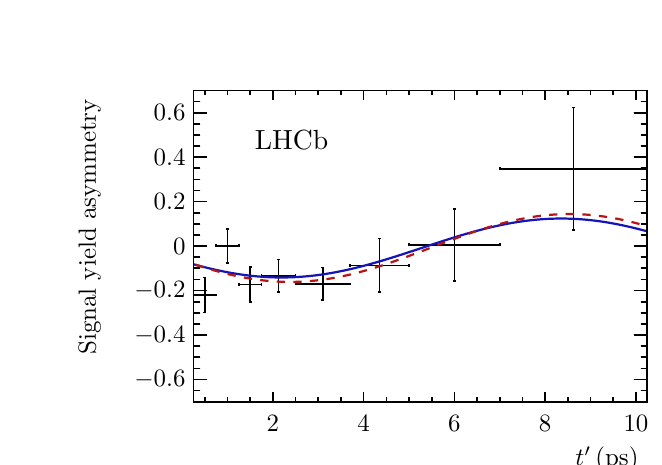
\begin{tikzpicture}[scale=0.38]
\pgfdeclareplotmark{cross} {
\pgfpathmoveto{\pgfpoint{-0.3\pgfplotmarksize}{\pgfplotmarksize}}
\pgfpathlineto{\pgfpoint{+0.3\pgfplotmarksize}{\pgfplotmarksize}}
\pgfpathlineto{\pgfpoint{+0.3\pgfplotmarksize}{0.3\pgfplotmarksize}}
\pgfpathlineto{\pgfpoint{+1\pgfplotmarksize}{0.3\pgfplotmarksize}}
\pgfpathlineto{\pgfpoint{+1\pgfplotmarksize}{-0.3\pgfplotmarksize}}
\pgfpathlineto{\pgfpoint{+0.3\pgfplotmarksize}{-0.3\pgfplotmarksize}}
\pgfpathlineto{\pgfpoint{+0.3\pgfplotmarksize}{-1.\pgfplotmarksize}}
\pgfpathlineto{\pgfpoint{-0.3\pgfplotmarksize}{-1.\pgfplotmarksize}}
\pgfpathlineto{\pgfpoint{-0.3\pgfplotmarksize}{-0.3\pgfplotmarksize}}
\pgfpathlineto{\pgfpoint{-1.\pgfplotmarksize}{-0.3\pgfplotmarksize}}
\pgfpathlineto{\pgfpoint{-1.\pgfplotmarksize}{0.3\pgfplotmarksize}}
\pgfpathlineto{\pgfpoint{-0.3\pgfplotmarksize}{0.3\pgfplotmarksize}}
\pgfpathclose
\pgfusepathqstroke
}
\pgfdeclareplotmark{cross*} {
\pgfpathmoveto{\pgfpoint{-0.3\pgfplotmarksize}{\pgfplotmarksize}}
\pgfpathlineto{\pgfpoint{+0.3\pgfplotmarksize}{\pgfplotmarksize}}
\pgfpathlineto{\pgfpoint{+0.3\pgfplotmarksize}{0.3\pgfplotmarksize}}
\pgfpathlineto{\pgfpoint{+1\pgfplotmarksize}{0.3\pgfplotmarksize}}
\pgfpathlineto{\pgfpoint{+1\pgfplotmarksize}{-0.3\pgfplotmarksize}}
\pgfpathlineto{\pgfpoint{+0.3\pgfplotmarksize}{-0.3\pgfplotmarksize}}
\pgfpathlineto{\pgfpoint{+0.3\pgfplotmarksize}{-1.\pgfplotmarksize}}
\pgfpathlineto{\pgfpoint{-0.3\pgfplotmarksize}{-1.\pgfplotmarksize}}
\pgfpathlineto{\pgfpoint{-0.3\pgfplotmarksize}{-0.3\pgfplotmarksize}}
\pgfpathlineto{\pgfpoint{-1.\pgfplotmarksize}{-0.3\pgfplotmarksize}}
\pgfpathlineto{\pgfpoint{-1.\pgfplotmarksize}{0.3\pgfplotmarksize}}
\pgfpathlineto{\pgfpoint{-0.3\pgfplotmarksize}{0.3\pgfplotmarksize}}
\pgfpathclose
\pgfusepathqfillstroke
}
\pgfdeclareplotmark{newstar} {
\pgfpathmoveto{\pgfqpoint{0pt}{\pgfplotmarksize}}
\pgfpathlineto{\pgfqpointpolar{44}{0.5\pgfplotmarksize}}
\pgfpathlineto{\pgfqpointpolar{18}{\pgfplotmarksize}}
\pgfpathlineto{\pgfqpointpolar{-20}{0.5\pgfplotmarksize}}
\pgfpathlineto{\pgfqpointpolar{-54}{\pgfplotmarksize}}
\pgfpathlineto{\pgfqpointpolar{-90}{0.5\pgfplotmarksize}}
\pgfpathlineto{\pgfqpointpolar{234}{\pgfplotmarksize}}
\pgfpathlineto{\pgfqpointpolar{198}{0.5\pgfplotmarksize}}
\pgfpathlineto{\pgfqpointpolar{162}{\pgfplotmarksize}}
\pgfpathlineto{\pgfqpointpolar{134}{0.5\pgfplotmarksize}}
\pgfpathclose
\pgfusepathqstroke
}
\pgfdeclareplotmark{newstar*} {
\pgfpathmoveto{\pgfqpoint{0pt}{\pgfplotmarksize}}
\pgfpathlineto{\pgfqpointpolar{44}{0.5\pgfplotmarksize}}
\pgfpathlineto{\pgfqpointpolar{18}{\pgfplotmarksize}}
\pgfpathlineto{\pgfqpointpolar{-20}{0.5\pgfplotmarksize}}
\pgfpathlineto{\pgfqpointpolar{-54}{\pgfplotmarksize}}
\pgfpathlineto{\pgfqpointpolar{-90}{0.5\pgfplotmarksize}}
\pgfpathlineto{\pgfqpointpolar{234}{\pgfplotmarksize}}
\pgfpathlineto{\pgfqpointpolar{198}{0.5\pgfplotmarksize}}
\pgfpathlineto{\pgfqpointpolar{162}{\pgfplotmarksize}}
\pgfpathlineto{\pgfqpointpolar{134}{0.5\pgfplotmarksize}}
\pgfpathclose
\pgfusepathqfillstroke
}
\definecolor{c}{rgb}{1,1,1};
\draw [color=c, fill=c] (0.4,0) rectangle (19.6,13.1687);
\draw [color=c, fill=c] (3.472,2.107) rectangle (18.64,12.5103);
\definecolor{c}{rgb}{0,0,0};
\draw [c,line width=0.6] (3.472,2.107) -- (3.472,12.5103) -- (18.64,12.5103) -- (18.64,2.107) -- (3.472,2.107);
\definecolor{c}{rgb}{1,1,1};
\draw [color=c, fill=c] (3.472,2.107) rectangle (18.64,12.5103);
\definecolor{c}{rgb}{0,0,0};
\draw [c,line width=0.6] (3.472,2.107) -- (3.472,12.5103) -- (18.64,12.5103) -- (18.64,2.107) -- (3.472,2.107);
\draw [c,line width=0.6] (3.472,2.107) -- (18.64,2.107);
\draw [anchor= east] (18.64,0.2) node[scale=0.9, color=c, rotate=0]{$t^\prime\,\mathrm{(ps)}$};
\draw [c,line width=0.6] (6.1264,2.4191) -- (6.1264,2.107);
\draw [c,line width=0.6] (6.8848,2.26305) -- (6.8848,2.107);
\draw [c,line width=0.6] (7.6432,2.26305) -- (7.6432,2.107);
\draw [c,line width=0.6] (8.4016,2.26305) -- (8.4016,2.107);
\draw [c,line width=0.6] (9.16,2.4191) -- (9.16,2.107);
\draw [c,line width=0.6] (9.9184,2.26305) -- (9.9184,2.107);
\draw [c,line width=0.6] (10.6768,2.26305) -- (10.6768,2.107);
\draw [c,line width=0.6] (11.4352,2.26305) -- (11.4352,2.107);
\draw [c,line width=0.6] (12.1936,2.4191) -- (12.1936,2.107);
\draw [c,line width=0.6] (12.952,2.26305) -- (12.952,2.107);
\draw [c,line width=0.6] (13.7104,2.26305) -- (13.7104,2.107);
\draw [c,line width=0.6] (14.4688,2.26305) -- (14.4688,2.107);
\draw [c,line width=0.6] (15.2272,2.4191) -- (15.2272,2.107);
\draw [c,line width=0.6] (15.9856,2.26305) -- (15.9856,2.107);
\draw [c,line width=0.6] (16.744,2.26305) -- (16.744,2.107);
\draw [c,line width=0.6] (17.5024,2.26305) -- (17.5024,2.107);
\draw [c,line width=0.6] (18.2608,2.4191) -- (18.2608,2.107);
\draw [c,line width=0.6] (6.1264,2.4191) -- (6.1264,2.107);
\draw [c,line width=0.6] (5.368,2.26305) -- (5.368,2.107);
\draw [c,line width=0.6] (4.6096,2.26305) -- (4.6096,2.107);
\draw [c,line width=0.6] (3.8512,2.26305) -- (3.8512,2.107);
\draw [c,line width=0.6] (18.2608,2.4191) -- (18.2608,2.107);
\draw [anchor=base] (6.1264,1.1) node[scale=0.9, color=c, rotate=0]{$2$};
\draw [anchor=base] (9.16,1.1) node[scale=0.9, color=c, rotate=0]{$4$};
\draw [anchor=base] (12.1936,1.1) node[scale=0.9, color=c, rotate=0]{$6$};
\draw [anchor=base] (15.2272,1.1) node[scale=0.9, color=c, rotate=0]{$8$};
\draw [anchor=base] (18.2608,1.1) node[scale=0.9, color=c, rotate=0]{$10$};
\draw [c,line width=0.6] (3.472,12.5103) -- (18.64,12.5103);
\draw [c,line width=0.6] (6.1264,12.1982) -- (6.1264,12.5103);
\draw [c,line width=0.6] (6.8848,12.3543) -- (6.8848,12.5103);
\draw [c,line width=0.6] (7.6432,12.3543) -- (7.6432,12.5103);
\draw [c,line width=0.6] (8.4016,12.3543) -- (8.4016,12.5103);
\draw [c,line width=0.6] (9.16,12.1982) -- (9.16,12.5103);
\draw [c,line width=0.6] (9.9184,12.3543) -- (9.9184,12.5103);
\draw [c,line width=0.6] (10.6768,12.3543) -- (10.6768,12.5103);
\draw [c,line width=0.6] (11.4352,12.3543) -- (11.4352,12.5103);
\draw [c,line width=0.6] (12.1936,12.1982) -- (12.1936,12.5103);
\draw [c,line width=0.6] (12.952,12.3543) -- (12.952,12.5103);
\draw [c,line width=0.6] (13.7104,12.3543) -- (13.7104,12.5103);
\draw [c,line width=0.6] (14.4688,12.3543) -- (14.4688,12.5103);
\draw [c,line width=0.6] (15.2272,12.1982) -- (15.2272,12.5103);
\draw [c,line width=0.6] (15.9856,12.3543) -- (15.9856,12.5103);
\draw [c,line width=0.6] (16.744,12.3543) -- (16.744,12.5103);
\draw [c,line width=0.6] (17.5024,12.3543) -- (17.5024,12.5103);
\draw [c,line width=0.6] (18.2608,12.1982) -- (18.2608,12.5103);
\draw [c,line width=0.6] (6.1264,12.1982) -- (6.1264,12.5103);
\draw [c,line width=0.6] (5.368,12.3543) -- (5.368,12.5103);
\draw [c,line width=0.6] (4.6096,12.3543) -- (4.6096,12.5103);
\draw [c,line width=0.6] (3.8512,12.3543) -- (3.8512,12.5103);
\draw [c,line width=0.6] (18.2608,12.1982) -- (18.2608,12.5103);
\draw [c,line width=0.6] (3.472,2.107) -- (3.472,12.5103);
\draw [anchor= east] (0.,12.5103) node[scale=0.9, color=c, rotate=90]{Signal yield asymmetry};
\draw [c,line width=0.6] (3.92704,2.85009) -- (3.472,2.85009);
\draw [c,line width=0.6] (3.69952,3.22164) -- (3.472,3.22164);
\draw [c,line width=0.6] (3.69952,3.59319) -- (3.472,3.59319);
\draw [c,line width=0.6] (3.69952,3.96473) -- (3.472,3.96473);
\draw [c,line width=0.6] (3.92704,4.33628) -- (3.472,4.33628);
\draw [c,line width=0.6] (3.69952,4.70783) -- (3.472,4.70783);
\draw [c,line width=0.6] (3.69952,5.07937) -- (3.472,5.07937);
\draw [c,line width=0.6] (3.69952,5.45092) -- (3.472,5.45092);
\draw [c,line width=0.6] (3.92704,5.82247) -- (3.472,5.82247);
\draw [c,line width=0.6] (3.69952,6.19402) -- (3.472,6.19402);
\draw [c,line width=0.6] (3.69952,6.56556) -- (3.472,6.56556);
\draw [c,line width=0.6] (3.69952,6.93711) -- (3.472,6.93711);
\draw [c,line width=0.6] (3.92704,7.30866) -- (3.472,7.30866);
\draw [c,line width=0.6] (3.69952,7.6802) -- (3.472,7.6802);
\draw [c,line width=0.6] (3.69952,8.05175) -- (3.472,8.05175);
\draw [c,line width=0.6] (3.69952,8.4233) -- (3.472,8.4233);
\draw [c,line width=0.6] (3.92704,8.79484) -- (3.472,8.79484);
\draw [c,line width=0.6] (3.69952,9.16639) -- (3.472,9.16639);
\draw [c,line width=0.6] (3.69952,9.53794) -- (3.472,9.53794);
\draw [c,line width=0.6] (3.69952,9.90948) -- (3.472,9.90948);
\draw [c,line width=0.6] (3.92704,10.281) -- (3.472,10.281);
\draw [c,line width=0.6] (3.69952,10.6526) -- (3.472,10.6526);
\draw [c,line width=0.6] (3.69952,11.0241) -- (3.472,11.0241);
\draw [c,line width=0.6] (3.69952,11.3957) -- (3.472,11.3957);
\draw [c,line width=0.6] (3.92704,11.7672) -- (3.472,11.7672);
\draw [c,line width=0.6] (3.92704,2.85009) -- (3.472,2.85009);
\draw [c,line width=0.6] (3.69952,2.47855) -- (3.472,2.47855);
\draw [c,line width=0.6] (3.92704,11.7672) -- (3.472,11.7672);
\draw [c,line width=0.6] (3.69952,12.1388) -- (3.472,12.1388);
\draw [anchor= east] (3.5,2.85009) node[scale=0.9, color=c, rotate=0]{$-0.6$};
\draw [anchor= east] (3.5,4.33628) node[scale=0.9, color=c, rotate=0]{$-0.4$};
\draw [anchor= east] (3.5,5.82247) node[scale=0.9, color=c, rotate=0]{$-0.2$};
\draw [anchor= east] (3.5,7.30866) node[scale=0.9, color=c, rotate=0]{$0$};
\draw [anchor= east] (3.5,8.79484) node[scale=0.9, color=c, rotate=0]{$0.2$};
\draw [anchor= east] (3.5,10.281) node[scale=0.9, color=c, rotate=0]{$0.4$};
\draw [anchor= east] (3.5,11.7672) node[scale=0.9, color=c, rotate=0]{$0.6$};
\draw [c,line width=0.6] (18.64,2.107) -- (18.64,12.5103);
\draw [c,line width=0.6] (18.185,2.85009) -- (18.64,2.85009);
\draw [c,line width=0.6] (18.4125,3.22164) -- (18.64,3.22164);
\draw [c,line width=0.6] (18.4125,3.59319) -- (18.64,3.59319);
\draw [c,line width=0.6] (18.4125,3.96473) -- (18.64,3.96473);
\draw [c,line width=0.6] (18.185,4.33628) -- (18.64,4.33628);
\draw [c,line width=0.6] (18.4125,4.70783) -- (18.64,4.70783);
\draw [c,line width=0.6] (18.4125,5.07937) -- (18.64,5.07937);
\draw [c,line width=0.6] (18.4125,5.45092) -- (18.64,5.45092);
\draw [c,line width=0.6] (18.185,5.82247) -- (18.64,5.82247);
\draw [c,line width=0.6] (18.4125,6.19402) -- (18.64,6.19402);
\draw [c,line width=0.6] (18.4125,6.56556) -- (18.64,6.56556);
\draw [c,line width=0.6] (18.4125,6.93711) -- (18.64,6.93711);
\draw [c,line width=0.6] (18.185,7.30866) -- (18.64,7.30866);
\draw [c,line width=0.6] (18.4125,7.6802) -- (18.64,7.6802);
\draw [c,line width=0.6] (18.4125,8.05175) -- (18.64,8.05175);
\draw [c,line width=0.6] (18.4125,8.4233) -- (18.64,8.4233);
\draw [c,line width=0.6] (18.185,8.79484) -- (18.64,8.79484);
\draw [c,line width=0.6] (18.4125,9.16639) -- (18.64,9.16639);
\draw [c,line width=0.6] (18.4125,9.53794) -- (18.64,9.53794);
\draw [c,line width=0.6] (18.4125,9.90948) -- (18.64,9.90948);
\draw [c,line width=0.6] (18.185,10.281) -- (18.64,10.281);
\draw [c,line width=0.6] (18.4125,10.6526) -- (18.64,10.6526);
\draw [c,line width=0.6] (18.4125,11.0241) -- (18.64,11.0241);
\draw [c,line width=0.6] (18.4125,11.3957) -- (18.64,11.3957);
\draw [c,line width=0.6] (18.185,11.7672) -- (18.64,11.7672);
\draw [c,line width=0.6] (18.185,2.85009) -- (18.64,2.85009);
\draw [c,line width=0.6] (18.4125,2.47855) -- (18.64,2.47855);
\draw [c,line width=0.6] (18.185,11.7672) -- (18.64,11.7672);
\draw [c,line width=0.6] (18.4125,12.1388) -- (18.64,12.1388);
\draw [c,line width=0.6] (3.8512,5.67382) -- (3.472,5.67382);
\draw [c,line width=0.6] (3.472,5.62917) -- (3.472,5.71846);
\draw [c,line width=0.6] (3.8512,5.67382) -- (4.2304,5.67382);
\draw [c,line width=0.6] (4.2304,5.62917) -- (4.2304,5.71846);
\draw [c,line width=0.6] (3.8512,5.67382) -- (3.8512,6.26338);
\draw [c,line width=0.6] (3.80656,6.26338) -- (3.89584,6.26338);
\draw [c,line width=0.6] (3.8512,5.67382) -- (3.8512,5.08425);
\draw [c,line width=0.6] (3.80656,5.08425) -- (3.89584,5.08425);
\draw [c,line width=0.6] (4.6096,7.31799) -- (4.2304,7.31799);
\draw [c,line width=0.6] (4.2304,7.27334) -- (4.2304,7.36263);
\draw [c,line width=0.6] (4.6096,7.31799) -- (4.9888,7.31799);
\draw [c,line width=0.6] (4.9888,7.27334) -- (4.9888,7.36263);
\draw [c,line width=0.6] (4.6096,7.31799) -- (4.6096,7.88392);
\draw [c,line width=0.6] (4.56496,7.88392) -- (4.65424,7.88392);
\draw [c,line width=0.6] (4.6096,7.31799) -- (4.6096,6.75206);
\draw [c,line width=0.6] (4.56496,6.75206) -- (4.65424,6.75206);
\draw [c,line width=0.6] (5.368,6.02773) -- (4.9888,6.02773);
\draw [c,line width=0.6] (4.9888,5.98309) -- (4.9888,6.07237);
\draw [c,line width=0.6] (5.368,6.02773) -- (5.7472,6.02773);
\draw [c,line width=0.6] (5.7472,5.98309) -- (5.7472,6.07237);
\draw [c,line width=0.6] (5.368,6.02773) -- (5.368,6.60606);
\draw [c,line width=0.6] (5.32336,6.60606) -- (5.41264,6.60606);
\draw [c,line width=0.6] (5.368,6.02773) -- (5.368,5.4494);
\draw [c,line width=0.6] (5.32336,5.4494) -- (5.41264,5.4494);
\draw [c,line width=0.6] (6.316,6.31938) -- (5.7472,6.31938);
\draw [c,line width=0.6] (5.7472,6.27474) -- (5.7472,6.36403);
\draw [c,line width=0.6] (6.316,6.31938) -- (6.8848,6.31938);
\draw [c,line width=0.6] (6.8848,6.27474) -- (6.8848,6.36403);
\draw [c,line width=0.6] (6.316,6.31938) -- (6.316,6.85688);
\draw [c,line width=0.6] (6.27136,6.85688) -- (6.36064,6.85688);
\draw [c,line width=0.6] (6.316,6.31938) -- (6.316,5.78189);
\draw [c,line width=0.6] (6.27136,5.78189) -- (6.36064,5.78189);
\draw [c,line width=0.6] (7.79488,6.04513) -- (6.8848,6.04513);
\draw [c,line width=0.6] (6.8848,6.00049) -- (6.8848,6.08977);
\draw [c,line width=0.6] (7.79488,6.04513) -- (8.70496,6.04513);
\draw [c,line width=0.6] (8.70496,6.00049) -- (8.70496,6.08977);
\draw [c,line width=0.6] (7.79488,6.04513) -- (7.79488,6.58853);
\draw [c,line width=0.6] (7.75024,6.58853) -- (7.83952,6.58853);
\draw [c,line width=0.6] (7.79488,6.04513) -- (7.79488,5.50173);
\draw [c,line width=0.6] (7.75024,5.50173) -- (7.83952,5.50173);
\draw [c,line width=0.6] (9.69088,6.66455) -- (8.70496,6.66455);
\draw [c,line width=0.6] (8.70496,6.61991) -- (8.70496,6.7092);
\draw [c,line width=0.6] (9.69088,6.66455) -- (10.6768,6.66455);
\draw [c,line width=0.6] (10.6768,6.61991) -- (10.6768,6.7092);
\draw [c,line width=0.6] (9.69088,6.66455) -- (9.69088,7.55685);
\draw [c,line width=0.6] (9.64624,7.55685) -- (9.73552,7.55685);
\draw [c,line width=0.6] (9.69088,6.66455) -- (9.69088,5.77226);
\draw [c,line width=0.6] (9.64624,5.77226) -- (9.73552,5.77226);
\draw [c,line width=0.6] (12.1936,7.35236) -- (10.6768,7.35236);
\draw [c,line width=0.6] (10.6768,7.30772) -- (10.6768,7.39701);
\draw [c,line width=0.6] (12.1936,7.35236) -- (13.7104,7.35236);
\draw [c,line width=0.6] (13.7104,7.30772) -- (13.7104,7.39701);
\draw [c,line width=0.6] (12.1936,7.35236) -- (12.1936,8.55254);
\draw [c,line width=0.6] (12.149,8.55254) -- (12.2382,8.55254);
\draw [c,line width=0.6] (12.1936,7.35236) -- (12.1936,6.15218);
\draw [c,line width=0.6] (12.149,6.15218) -- (12.2382,6.15218);
\draw [c,line width=0.6] (16.1752,9.89514) -- (13.7104,9.89514);
\draw [c,line width=0.6] (13.7104,9.85049) -- (13.7104,9.93978);
\draw [c,line width=0.6] (16.1752,9.89514) -- (18.64,9.89514);
\draw [c,line width=0.6] (18.64,9.85049) -- (18.64,9.93978);
\draw [c,line width=0.6] (16.1752,9.89514) -- (16.1752,11.9447);
\draw [c,line width=0.6] (16.1306,11.9447) -- (16.2198,11.9447);
\draw [c,line width=0.6] (16.1752,9.89514) -- (16.1752,7.84559);
\draw [c,line width=0.6] (16.1306,7.84559) -- (16.2198,7.84559);
\foreach \P in {(3.8512,5.67382),(4.6096,7.31799),(5.368,6.02773),(6.316,6.31938),(7.79488,6.04513),(9.69088,6.66455),(12.1936,7.35236),(16.1752,9.89514)}{\draw[mark options={color=c,fill=c},mark size=2.402402pt,mark=] plot coordinates {\P};}
\definecolor{c}{rgb}{0.08,0.08,0.72};
\draw [c,line width=0.8] (3.472,6.7014) -- (3.62368,6.6603) -- (3.77536,6.62071) -- (3.92704,6.58274) -- (4.07872,6.5465) -- (4.2304,6.51206) -- (4.38208,6.47952) -- (4.53376,6.44897) -- (4.68544,6.42047) -- (4.83712,6.39411) -- (4.9888,6.36995) --
 (5.14048,6.34805) -- (5.29216,6.32847) -- (5.44384,6.31126) -- (5.59552,6.29647) -- (5.7472,6.28412) -- (5.89888,6.27426) -- (6.05056,6.2669) -- (6.20224,6.26208) -- (6.35392,6.25979) -- (6.5056,6.26004) -- (6.65728,6.26284) -- (6.80896,6.26817) --
 (6.96064,6.27603) -- (7.11232,6.28639) -- (7.264,6.29923) -- (7.41568,6.31451) -- (7.56736,6.33219) -- (7.71904,6.35224) -- (7.87072,6.37459) -- (8.0224,6.39919) -- (8.17408,6.42599) -- (8.32576,6.4549) -- (8.47744,6.48586) -- (8.62912,6.51878) --
 (8.7808,6.55358) -- (8.93248,6.59018) -- (9.08416,6.62848) -- (9.23584,6.66838) -- (9.38752,6.70977) -- (9.5392,6.75256) -- (9.69088,6.79662) -- (9.84256,6.84186) -- (9.99424,6.88814) -- (10.1459,6.93536) -- (10.2976,6.98338) -- (10.4493,7.03209) --
 (10.601,7.08136) -- (10.7526,7.13106) -- (10.9043,7.18106) -- (11.056,7.23124) -- (11.2077,7.28145) -- (11.3594,7.33158) -- (11.511,7.38149) -- (11.6627,7.43105) -- (11.8144,7.48014) -- (11.9661,7.52861) -- (12.1178,7.57636) -- (12.2694,7.62324) --
 (12.4211,7.66915) -- (12.5728,7.71395) -- (12.7245,7.75754) -- (12.8762,7.79979) -- (13.0278,7.8406) -- (13.1795,7.87986) -- (13.3312,7.91747) -- (13.4829,7.95332) -- (13.6346,7.98733) -- (13.7862,8.01939) -- (13.9379,8.04944) -- (14.0896,8.07738)
 -- (14.2413,8.10316) -- (14.393,8.12668) -- (14.5446,8.1479) -- (14.6963,8.16677) -- (14.848,8.18322) -- (14.9997,8.19721) -- (15.1514,8.20872) -- (15.303,8.2177) -- (15.4547,8.22414) -- (15.6064,8.22801) -- (15.7581,8.22931) -- (15.9098,8.22804) --
 (16.0614,8.22419) -- (16.2131,8.21778) -- (16.3648,8.20882) -- (16.5165,8.19734) -- (16.6682,8.18337) -- (16.8198,8.16694) -- (16.9715,8.1481) -- (17.1232,8.1269) -- (17.2749,8.1034) -- (17.4266,8.07765) -- (17.5782,8.04973) -- (17.7299,8.0197) --
 (17.8816,7.98765) -- (18.0333,7.95367) -- (18.185,7.91783) -- (18.3366,7.88024) -- (18.4883,7.841) -- (18.64,7.80021);
\definecolor{c}{rgb}{0.72,0.08,0.08};
\draw [c,dashed, line width=0.8] (3.54784,6.68696) -- (3.69952,6.63742) -- (3.8512,6.58946) -- (4.00288,6.5432) -- (4.15456,6.49877) -- (4.30624,6.45628) -- (4.45792,6.41583) -- (4.6096,6.37754) -- (4.76128,6.34149) -- (4.91296,6.30779) -- (5.06464,6.27651)
 -- (5.21632,6.24774) -- (5.368,6.22154) -- (5.51968,6.198) -- (5.67136,6.17716) -- (5.82304,6.15909) -- (5.97472,6.14381) -- (6.1264,6.13139) -- (6.27808,6.12184) -- (6.42976,6.11519) -- (6.58144,6.11146) -- (6.73312,6.11066) -- (6.8848,6.11279) --
 (7.03648,6.11784) -- (7.18816,6.1258) -- (7.33984,6.13666) -- (7.49152,6.15037) -- (7.6432,6.16692) -- (7.79488,6.18625) -- (7.94656,6.20832) -- (8.09824,6.23307) -- (8.24992,6.26044) -- (8.4016,6.29035) -- (8.55328,6.32274) -- (8.70496,6.35751) --
 (8.85664,6.39459) -- (9.00832,6.43387) -- (9.16,6.47526) -- (9.31168,6.51864) -- (9.46336,6.56391) -- (9.61504,6.61095) -- (9.76672,6.65964) -- (9.9184,6.70986) -- (10.0701,6.76147) -- (10.2218,6.81435) -- (10.3734,6.86835) -- (10.5251,6.92334) --
 (10.6768,6.97918) -- (10.8285,7.03572) -- (10.9802,7.09281) -- (11.1318,7.15031) -- (11.2835,7.20806) -- (11.4352,7.26593) -- (11.5869,7.32375) -- (11.7386,7.38138) -- (11.8902,7.43866) -- (12.0419,7.49545) -- (12.1936,7.5516) -- (12.3453,7.60696)
 -- (12.497,7.66139) -- (12.6486,7.71475) -- (12.8003,7.76689) -- (12.952,7.81767) -- (13.1037,7.86698) -- (13.2554,7.91466) -- (13.407,7.96061) -- (13.5587,8.00469) -- (13.7104,8.0468) -- (13.8621,8.08682) -- (14.0138,8.12464) -- (14.1654,8.16017)
 -- (14.3171,8.19331) -- (14.4688,8.22398) -- (14.6205,8.25209) -- (14.7722,8.27756) -- (14.9238,8.30034) -- (15.0755,8.32036) -- (15.2272,8.33756) -- (15.3789,8.35191) -- (15.5306,8.36336) -- (15.6822,8.37188) -- (15.8339,8.37746) --
 (15.9856,8.38007) -- (16.1373,8.37971) -- (16.289,8.37637) -- (16.4406,8.37008) -- (16.5923,8.36084) -- (16.744,8.34869) -- (16.8957,8.33364) -- (17.0474,8.31575) -- (17.199,8.29506) -- (17.3507,8.27162) -- (17.5024,8.24549) -- (17.6541,8.21676) --
 (17.8058,8.18548) -- (17.9574,8.15175) -- (18.1091,8.11566) -- (18.2608,8.07729) -- (18.4125,8.03675) -- (18.5642,7.99416);
\definecolor{c}{rgb}{0,0,0};
\draw [c,line width=0.6] (3.472,2.107) -- (18.64,2.107);
\draw [c,line width=0.6] (6.1264,2.4191) -- (6.1264,2.107);
\draw [c,line width=0.6] (6.8848,2.26305) -- (6.8848,2.107);
\draw [c,line width=0.6] (7.6432,2.26305) -- (7.6432,2.107);
\draw [c,line width=0.6] (8.4016,2.26305) -- (8.4016,2.107);
\draw [c,line width=0.6] (9.16,2.4191) -- (9.16,2.107);
\draw [c,line width=0.6] (9.9184,2.26305) -- (9.9184,2.107);
\draw [c,line width=0.6] (10.6768,2.26305) -- (10.6768,2.107);
\draw [c,line width=0.6] (11.4352,2.26305) -- (11.4352,2.107);
\draw [c,line width=0.6] (12.1936,2.4191) -- (12.1936,2.107);
\draw [c,line width=0.6] (12.952,2.26305) -- (12.952,2.107);
\draw [c,line width=0.6] (13.7104,2.26305) -- (13.7104,2.107);
\draw [c,line width=0.6] (14.4688,2.26305) -- (14.4688,2.107);
\draw [c,line width=0.6] (15.2272,2.4191) -- (15.2272,2.107);
\draw [c,line width=0.6] (15.9856,2.26305) -- (15.9856,2.107);
\draw [c,line width=0.6] (16.744,2.26305) -- (16.744,2.107);
\draw [c,line width=0.6] (17.5024,2.26305) -- (17.5024,2.107);
\draw [c,line width=0.6] (18.2608,2.4191) -- (18.2608,2.107);
\draw [c,line width=0.6] (6.1264,2.4191) -- (6.1264,2.107);
\draw [c,line width=0.6] (5.368,2.26305) -- (5.368,2.107);
\draw [c,line width=0.6] (4.6096,2.26305) -- (4.6096,2.107);
\draw [c,line width=0.6] (3.8512,2.26305) -- (3.8512,2.107);
\draw [c,line width=0.6] (18.2608,2.4191) -- (18.2608,2.107);
\draw [c,line width=0.6] (3.472,12.5103) -- (18.64,12.5103);
\draw [c,line width=0.6] (6.1264,12.1982) -- (6.1264,12.5103);
\draw [c,line width=0.6] (6.8848,12.3543) -- (6.8848,12.5103);
\draw [c,line width=0.6] (7.6432,12.3543) -- (7.6432,12.5103);
\draw [c,line width=0.6] (8.4016,12.3543) -- (8.4016,12.5103);
\draw [c,line width=0.6] (9.16,12.1982) -- (9.16,12.5103);
\draw [c,line width=0.6] (9.9184,12.3543) -- (9.9184,12.5103);
\draw [c,line width=0.6] (10.6768,12.3543) -- (10.6768,12.5103);
\draw [c,line width=0.6] (11.4352,12.3543) -- (11.4352,12.5103);
\draw [c,line width=0.6] (12.1936,12.1982) -- (12.1936,12.5103);
\draw [c,line width=0.6] (12.952,12.3543) -- (12.952,12.5103);
\draw [c,line width=0.6] (13.7104,12.3543) -- (13.7104,12.5103);
\draw [c,line width=0.6] (14.4688,12.3543) -- (14.4688,12.5103);
\draw [c,line width=0.6] (15.2272,12.1982) -- (15.2272,12.5103);
\draw [c,line width=0.6] (15.9856,12.3543) -- (15.9856,12.5103);
\draw [c,line width=0.6] (16.744,12.3543) -- (16.744,12.5103);
\draw [c,line width=0.6] (17.5024,12.3543) -- (17.5024,12.5103);
\draw [c,line width=0.6] (18.2608,12.1982) -- (18.2608,12.5103);
\draw [c,line width=0.6] (6.1264,12.1982) -- (6.1264,12.5103);
\draw [c,line width=0.6] (5.368,12.3543) -- (5.368,12.5103);
\draw [c,line width=0.6] (4.6096,12.3543) -- (4.6096,12.5103);
\draw [c,line width=0.6] (3.8512,12.3543) -- (3.8512,12.5103);
\draw [c,line width=0.6] (18.2608,12.1982) -- (18.2608,12.5103);
\draw [c,line width=0.6] (3.472,2.107) -- (3.472,12.5103);
\draw [c,line width=0.6] (3.92704,2.85009) -- (3.472,2.85009);
\draw [c,line width=0.6] (3.69952,3.22164) -- (3.472,3.22164);
\draw [c,line width=0.6] (3.69952,3.59319) -- (3.472,3.59319);
\draw [c,line width=0.6] (3.69952,3.96473) -- (3.472,3.96473);
\draw [c,line width=0.6] (3.92704,4.33628) -- (3.472,4.33628);
\draw [c,line width=0.6] (3.69952,4.70783) -- (3.472,4.70783);
\draw [c,line width=0.6] (3.69952,5.07937) -- (3.472,5.07937);
\draw [c,line width=0.6] (3.69952,5.45092) -- (3.472,5.45092);
\draw [c,line width=0.6] (3.92704,5.82247) -- (3.472,5.82247);
\draw [c,line width=0.6] (3.69952,6.19402) -- (3.472,6.19402);
\draw [c,line width=0.6] (3.69952,6.56556) -- (3.472,6.56556);
\draw [c,line width=0.6] (3.69952,6.93711) -- (3.472,6.93711);
\draw [c,line width=0.6] (3.92704,7.30866) -- (3.472,7.30866);
\draw [c,line width=0.6] (3.69952,7.6802) -- (3.472,7.6802);
\draw [c,line width=0.6] (3.69952,8.05175) -- (3.472,8.05175);
\draw [c,line width=0.6] (3.69952,8.4233) -- (3.472,8.4233);
\draw [c,line width=0.6] (3.92704,8.79484) -- (3.472,8.79484);
\draw [c,line width=0.6] (3.69952,9.16639) -- (3.472,9.16639);
\draw [c,line width=0.6] (3.69952,9.53794) -- (3.472,9.53794);
\draw [c,line width=0.6] (3.69952,9.90948) -- (3.472,9.90948);
\draw [c,line width=0.6] (3.92704,10.281) -- (3.472,10.281);
\draw [c,line width=0.6] (3.69952,10.6526) -- (3.472,10.6526);
\draw [c,line width=0.6] (3.69952,11.0241) -- (3.472,11.0241);
\draw [c,line width=0.6] (3.69952,11.3957) -- (3.472,11.3957);
\draw [c,line width=0.6] (3.92704,11.7672) -- (3.472,11.7672);
\draw [c,line width=0.6] (3.92704,2.85009) -- (3.472,2.85009);
\draw [c,line width=0.6] (3.69952,2.47855) -- (3.472,2.47855);
\draw [c,line width=0.6] (3.92704,11.7672) -- (3.472,11.7672);
\draw [c,line width=0.6] (3.69952,12.1388) -- (3.472,12.1388);
\draw [c,line width=0.6] (18.64,2.107) -- (18.64,12.5103);
\draw [c,line width=0.6] (18.185,2.85009) -- (18.64,2.85009);
\draw [c,line width=0.6] (18.4125,3.22164) -- (18.64,3.22164);
\draw [c,line width=0.6] (18.4125,3.59319) -- (18.64,3.59319);
\draw [c,line width=0.6] (18.4125,3.96473) -- (18.64,3.96473);
\draw [c,line width=0.6] (18.185,4.33628) -- (18.64,4.33628);
\draw [c,line width=0.6] (18.4125,4.70783) -- (18.64,4.70783);
\draw [c,line width=0.6] (18.4125,5.07937) -- (18.64,5.07937);
\draw [c,line width=0.6] (18.4125,5.45092) -- (18.64,5.45092);
\draw [c,line width=0.6] (18.185,5.82247) -- (18.64,5.82247);
\draw [c,line width=0.6] (18.4125,6.19402) -- (18.64,6.19402);
\draw [c,line width=0.6] (18.4125,6.56556) -- (18.64,6.56556);
\draw [c,line width=0.6] (18.4125,6.93711) -- (18.64,6.93711);
\draw [c,line width=0.6] (18.185,7.30866) -- (18.64,7.30866);
\draw [c,line width=0.6] (18.4125,7.6802) -- (18.64,7.6802);
\draw [c,line width=0.6] (18.4125,8.05175) -- (18.64,8.05175);
\draw [c,line width=0.6] (18.4125,8.4233) -- (18.64,8.4233);
\draw [c,line width=0.6] (18.185,8.79484) -- (18.64,8.79484);
\draw [c,line width=0.6] (18.4125,9.16639) -- (18.64,9.16639);
\draw [c,line width=0.6] (18.4125,9.53794) -- (18.64,9.53794);
\draw [c,line width=0.6] (18.4125,9.90948) -- (18.64,9.90948);
\draw [c,line width=0.6] (18.185,10.281) -- (18.64,10.281);
\draw [c,line width=0.6] (18.4125,10.6526) -- (18.64,10.6526);
\draw [c,line width=0.6] (18.4125,11.0241) -- (18.64,11.0241);
\draw [c,line width=0.6] (18.4125,11.3957) -- (18.64,11.3957);
\draw [c,line width=0.6] (18.185,11.7672) -- (18.64,11.7672);
\draw [c,line width=0.6] (18.185,2.85009) -- (18.64,2.85009);
\draw [c,line width=0.6] (18.4125,2.47855) -- (18.64,2.47855);
\draw [c,line width=0.6] (18.185,11.7672) -- (18.64,11.7672);
\draw [c,line width=0.6] (18.4125,12.1388) -- (18.64,12.1388);
\draw [anchor=base west] (5.2,10.535) node[scale=1, color=c, rotate=0]{LHCb};

\end{tikzpicture}
\endpgfgraphicnamed

\beginpgfgraphicnamed{pdf/Likelihoodscan_C}
\begin{tikzpicture}[scale=0.38]
\begin{tikzpicture}
\pgfdeclareplotmark{cross} {
\pgfpathmoveto{\pgfpoint{-0.3\pgfplotmarksize}{\pgfplotmarksize}}
\pgfpathlineto{\pgfpoint{+0.3\pgfplotmarksize}{\pgfplotmarksize}}
\pgfpathlineto{\pgfpoint{+0.3\pgfplotmarksize}{0.3\pgfplotmarksize}}
\pgfpathlineto{\pgfpoint{+1\pgfplotmarksize}{0.3\pgfplotmarksize}}
\pgfpathlineto{\pgfpoint{+1\pgfplotmarksize}{-0.3\pgfplotmarksize}}
\pgfpathlineto{\pgfpoint{+0.3\pgfplotmarksize}{-0.3\pgfplotmarksize}}
\pgfpathlineto{\pgfpoint{+0.3\pgfplotmarksize}{-1.\pgfplotmarksize}}
\pgfpathlineto{\pgfpoint{-0.3\pgfplotmarksize}{-1.\pgfplotmarksize}}
\pgfpathlineto{\pgfpoint{-0.3\pgfplotmarksize}{-0.3\pgfplotmarksize}}
\pgfpathlineto{\pgfpoint{-1.\pgfplotmarksize}{-0.3\pgfplotmarksize}}
\pgfpathlineto{\pgfpoint{-1.\pgfplotmarksize}{0.3\pgfplotmarksize}}
\pgfpathlineto{\pgfpoint{-0.3\pgfplotmarksize}{0.3\pgfplotmarksize}}
\pgfpathclose
\pgfusepathqstroke
}
\pgfdeclareplotmark{cross*} {
\pgfpathmoveto{\pgfpoint{-0.3\pgfplotmarksize}{\pgfplotmarksize}}
\pgfpathlineto{\pgfpoint{+0.3\pgfplotmarksize}{\pgfplotmarksize}}
\pgfpathlineto{\pgfpoint{+0.3\pgfplotmarksize}{0.3\pgfplotmarksize}}
\pgfpathlineto{\pgfpoint{+1\pgfplotmarksize}{0.3\pgfplotmarksize}}
\pgfpathlineto{\pgfpoint{+1\pgfplotmarksize}{-0.3\pgfplotmarksize}}
\pgfpathlineto{\pgfpoint{+0.3\pgfplotmarksize}{-0.3\pgfplotmarksize}}
\pgfpathlineto{\pgfpoint{+0.3\pgfplotmarksize}{-1.\pgfplotmarksize}}
\pgfpathlineto{\pgfpoint{-0.3\pgfplotmarksize}{-1.\pgfplotmarksize}}
\pgfpathlineto{\pgfpoint{-0.3\pgfplotmarksize}{-0.3\pgfplotmarksize}}
\pgfpathlineto{\pgfpoint{-1.\pgfplotmarksize}{-0.3\pgfplotmarksize}}
\pgfpathlineto{\pgfpoint{-1.\pgfplotmarksize}{0.3\pgfplotmarksize}}
\pgfpathlineto{\pgfpoint{-0.3\pgfplotmarksize}{0.3\pgfplotmarksize}}
\pgfpathclose
\pgfusepathqfillstroke
}
\pgfdeclareplotmark{newstar} {
\pgfpathmoveto{\pgfqpoint{0pt}{\pgfplotmarksize}}
\pgfpathlineto{\pgfqpointpolar{44}{0.5\pgfplotmarksize}}
\pgfpathlineto{\pgfqpointpolar{18}{\pgfplotmarksize}}
\pgfpathlineto{\pgfqpointpolar{-20}{0.5\pgfplotmarksize}}
\pgfpathlineto{\pgfqpointpolar{-54}{\pgfplotmarksize}}
\pgfpathlineto{\pgfqpointpolar{-90}{0.5\pgfplotmarksize}}
\pgfpathlineto{\pgfqpointpolar{234}{\pgfplotmarksize}}
\pgfpathlineto{\pgfqpointpolar{198}{0.5\pgfplotmarksize}}
\pgfpathlineto{\pgfqpointpolar{162}{\pgfplotmarksize}}
\pgfpathlineto{\pgfqpointpolar{134}{0.5\pgfplotmarksize}}
\pgfpathclose
\pgfusepathqstroke
}
\pgfdeclareplotmark{newstar*} {
\pgfpathmoveto{\pgfqpoint{0pt}{\pgfplotmarksize}}
\pgfpathlineto{\pgfqpointpolar{44}{0.5\pgfplotmarksize}}
\pgfpathlineto{\pgfqpointpolar{18}{\pgfplotmarksize}}
\pgfpathlineto{\pgfqpointpolar{-20}{0.5\pgfplotmarksize}}
\pgfpathlineto{\pgfqpointpolar{-54}{\pgfplotmarksize}}
\pgfpathlineto{\pgfqpointpolar{-90}{0.5\pgfplotmarksize}}
\pgfpathlineto{\pgfqpointpolar{234}{\pgfplotmarksize}}
\pgfpathlineto{\pgfqpointpolar{198}{0.5\pgfplotmarksize}}
\pgfpathlineto{\pgfqpointpolar{162}{\pgfplotmarksize}}
\pgfpathlineto{\pgfqpointpolar{134}{0.5\pgfplotmarksize}}
\pgfpathclose
\pgfusepathqfillstroke
}
\definecolor{c}{rgb}{1,1,1};
\draw [color=c, fill=c] (0.4,0) rectangle (19.6,13.1687);
\draw [color=c, fill=c] (3.472,2.107) rectangle (18.64,12.5103);
\definecolor{c}{rgb}{0,0,0};
\draw [c,line width=0.6] (3.472,2.107) -- (3.472,12.5103) -- (18.64,12.5103) -- (18.64,2.107) -- (3.472,2.107);
\definecolor{c}{rgb}{1,1,1};
\draw [color=c, fill=c] (3.472,2.107) rectangle (18.64,12.5103);
\definecolor{c}{rgb}{0,0,0};
\draw [c,line width=0.6] (3.472,2.107) -- (3.472,12.5103) -- (18.64,12.5103) -- (18.64,2.107) -- (3.472,2.107);
\draw [c,line width=0.6] (3.472,2.107) -- (18.64,2.107);
\draw [anchor= east] (18.64,0.665812) node[scale=2.08555, color=c, rotate=0]{$\CDD$};
\draw [c,line width=0.6] (3.95838,2.4191) -- (3.95838,2.107);
\draw [c,line width=0.6] (4.72068,2.26305) -- (4.72068,2.107);
\draw [c,line width=0.6] (5.48298,2.26305) -- (5.48298,2.107);
\draw [c,line width=0.6] (6.24527,2.26305) -- (6.24527,2.107);
\draw [c,line width=0.6] (7.00757,2.4191) -- (7.00757,2.107);
\draw [c,line width=0.6] (7.76986,2.26305) -- (7.76986,2.107);
\draw [c,line width=0.6] (8.53216,2.26305) -- (8.53216,2.107);
\draw [c,line width=0.6] (9.29446,2.26305) -- (9.29446,2.107);
\draw [c,line width=0.6] (10.0568,2.4191) -- (10.0568,2.107);
\draw [c,line width=0.6] (10.819,2.26305) -- (10.819,2.107);
\draw [c,line width=0.6] (11.5813,2.26305) -- (11.5813,2.107);
\draw [c,line width=0.6] (12.3436,2.26305) -- (12.3436,2.107);
\draw [c,line width=0.6] (13.1059,2.4191) -- (13.1059,2.107);
\draw [c,line width=0.6] (13.8682,2.26305) -- (13.8682,2.107);
\draw [c,line width=0.6] (14.6305,2.26305) -- (14.6305,2.107);
\draw [c,line width=0.6] (15.3928,2.26305) -- (15.3928,2.107);
\draw [c,line width=0.6] (16.1551,2.4191) -- (16.1551,2.107);
\draw [c,line width=0.6] (3.95838,2.4191) -- (3.95838,2.107);
\draw [c,line width=0.6] (16.1551,2.4191) -- (16.1551,2.107);
\draw [c,line width=0.6] (16.9174,2.26305) -- (16.9174,2.107);
\draw [c,line width=0.6] (17.6797,2.26305) -- (17.6797,2.107);
\draw [c,line width=0.6] (18.442,2.26305) -- (18.442,2.107);
\draw [anchor=base] (3.95838,1.34321) node[scale=1.73796, color=c, rotate=0]{-0.2};
\draw [anchor=base] (7.00757,1.34321) node[scale=1.73796, color=c, rotate=0]{0};
\draw [anchor=base] (10.0568,1.34321) node[scale=1.73796, color=c, rotate=0]{0.2};
\draw [anchor=base] (13.1059,1.34321) node[scale=1.73796, color=c, rotate=0]{0.4};
\draw [anchor=base] (16.1551,1.34321) node[scale=1.73796, color=c, rotate=0]{0.6};
\draw [c,line width=0.6] (3.472,12.5103) -- (18.64,12.5103);
\draw [c,line width=0.6] (3.95838,12.1982) -- (3.95838,12.5103);
\draw [c,line width=0.6] (4.72068,12.3543) -- (4.72068,12.5103);
\draw [c,line width=0.6] (5.48298,12.3543) -- (5.48298,12.5103);
\draw [c,line width=0.6] (6.24527,12.3543) -- (6.24527,12.5103);
\draw [c,line width=0.6] (7.00757,12.1982) -- (7.00757,12.5103);
\draw [c,line width=0.6] (7.76986,12.3543) -- (7.76986,12.5103);
\draw [c,line width=0.6] (8.53216,12.3543) -- (8.53216,12.5103);
\draw [c,line width=0.6] (9.29446,12.3543) -- (9.29446,12.5103);
\draw [c,line width=0.6] (10.0568,12.1982) -- (10.0568,12.5103);
\draw [c,line width=0.6] (10.819,12.3543) -- (10.819,12.5103);
\draw [c,line width=0.6] (11.5813,12.3543) -- (11.5813,12.5103);
\draw [c,line width=0.6] (12.3436,12.3543) -- (12.3436,12.5103);
\draw [c,line width=0.6] (13.1059,12.1982) -- (13.1059,12.5103);
\draw [c,line width=0.6] (13.8682,12.3543) -- (13.8682,12.5103);
\draw [c,line width=0.6] (14.6305,12.3543) -- (14.6305,12.5103);
\draw [c,line width=0.6] (15.3928,12.3543) -- (15.3928,12.5103);
\draw [c,line width=0.6] (16.1551,12.1982) -- (16.1551,12.5103);
\draw [c,line width=0.6] (3.95838,12.1982) -- (3.95838,12.5103);
\draw [c,line width=0.6] (16.1551,12.1982) -- (16.1551,12.5103);
\draw [c,line width=0.6] (16.9174,12.3543) -- (16.9174,12.5103);
\draw [c,line width=0.6] (17.6797,12.3543) -- (17.6797,12.5103);
\draw [c,line width=0.6] (18.442,12.3543) -- (18.442,12.5103);
\draw [c,line width=0.6] (3.472,2.107) -- (3.472,12.5103);
\draw [anchor= east] (2,12.5103) node[scale=1.93658, color=c, rotate=90]{$\Delta$ LL};
\draw [c,line width=0.6] (3.92704,2.57988) -- (3.472,2.57988);
\draw [c,line width=0.6] (3.69952,2.97462) -- (3.472,2.97462);
\draw [c,line width=0.6] (3.69952,3.36937) -- (3.472,3.36937);
\draw [c,line width=0.6] (3.69952,3.76411) -- (3.472,3.76411);
\draw [c,line width=0.6] (3.69952,4.15885) -- (3.472,4.15885);
\draw [c,line width=0.6] (3.92704,4.55359) -- (3.472,4.55359);
\draw [c,line width=0.6] (3.69952,4.94833) -- (3.472,4.94833);
\draw [c,line width=0.6] (3.69952,5.34308) -- (3.472,5.34308);
\draw [c,line width=0.6] (3.69952,5.73782) -- (3.472,5.73782);
\draw [c,line width=0.6] (3.69952,6.13256) -- (3.472,6.13256);
\draw [c,line width=0.6] (3.92704,6.5273) -- (3.472,6.5273);
\draw [c,line width=0.6] (3.69952,6.92204) -- (3.472,6.92204);
\draw [c,line width=0.6] (3.69952,7.31679) -- (3.472,7.31679);
\draw [c,line width=0.6] (3.69952,7.71153) -- (3.472,7.71153);
\draw [c,line width=0.6] (3.69952,8.10627) -- (3.472,8.10627);
\draw [c,line width=0.6] (3.92704,8.50101) -- (3.472,8.50101);
\draw [c,line width=0.6] (3.69952,8.89575) -- (3.472,8.89575);
\draw [c,line width=0.6] (3.69952,9.2905) -- (3.472,9.2905);
\draw [c,line width=0.6] (3.69952,9.68524) -- (3.472,9.68524);
\draw [c,line width=0.6] (3.69952,10.08) -- (3.472,10.08);
\draw [c,line width=0.6] (3.92704,10.4747) -- (3.472,10.4747);
\draw [c,line width=0.6] (3.69952,10.8695) -- (3.472,10.8695);
\draw [c,line width=0.6] (3.69952,11.2642) -- (3.472,11.2642);
\draw [c,line width=0.6] (3.69952,11.6589) -- (3.472,11.6589);
\draw [c,line width=0.6] (3.69952,12.0537) -- (3.472,12.0537);
\draw [c,line width=0.6] (3.92704,12.4484) -- (3.472,12.4484);
\draw [c,line width=0.6] (3.92704,2.57988) -- (3.472,2.57988);
\draw [c,line width=0.6] (3.69952,2.18514) -- (3.472,2.18514);
\draw [c,line width=0.6] (3.92704,12.4484) -- (3.472,12.4484);
\draw [anchor= east] (3.28,2.57988) node[scale=1.73796, color=c, rotate=0]{0};
\draw [anchor= east] (3.28,4.55359) node[scale=1.73796, color=c, rotate=0]{1};
\draw [anchor= east] (3.28,6.5273) node[scale=1.73796, color=c, rotate=0]{2};
\draw [anchor= east] (3.28,8.50101) node[scale=1.73796, color=c, rotate=0]{3};
\draw [anchor= east] (3.28,10.4747) node[scale=1.73796, color=c, rotate=0]{4};
\draw [anchor= east] (3.28,12.4484) node[scale=1.73796, color=c, rotate=0]{5};
\draw [c,line width=0.6] (18.64,2.107) -- (18.64,12.5103);
\draw [c,line width=0.6] (18.185,2.57988) -- (18.64,2.57988);
\draw [c,line width=0.6] (18.4125,2.97462) -- (18.64,2.97462);
\draw [c,line width=0.6] (18.4125,3.36937) -- (18.64,3.36937);
\draw [c,line width=0.6] (18.4125,3.76411) -- (18.64,3.76411);
\draw [c,line width=0.6] (18.4125,4.15885) -- (18.64,4.15885);
\draw [c,line width=0.6] (18.185,4.55359) -- (18.64,4.55359);
\draw [c,line width=0.6] (18.4125,4.94833) -- (18.64,4.94833);
\draw [c,line width=0.6] (18.4125,5.34308) -- (18.64,5.34308);
\draw [c,line width=0.6] (18.4125,5.73782) -- (18.64,5.73782);
\draw [c,line width=0.6] (18.4125,6.13256) -- (18.64,6.13256);
\draw [c,line width=0.6] (18.185,6.5273) -- (18.64,6.5273);
\draw [c,line width=0.6] (18.4125,6.92204) -- (18.64,6.92204);
\draw [c,line width=0.6] (18.4125,7.31679) -- (18.64,7.31679);
\draw [c,line width=0.6] (18.4125,7.71153) -- (18.64,7.71153);
\draw [c,line width=0.6] (18.4125,8.10627) -- (18.64,8.10627);
\draw [c,line width=0.6] (18.185,8.50101) -- (18.64,8.50101);
\draw [c,line width=0.6] (18.4125,8.89575) -- (18.64,8.89575);
\draw [c,line width=0.6] (18.4125,9.2905) -- (18.64,9.2905);
\draw [c,line width=0.6] (18.4125,9.68524) -- (18.64,9.68524);
\draw [c,line width=0.6] (18.4125,10.08) -- (18.64,10.08);
\draw [c,line width=0.6] (18.185,10.4747) -- (18.64,10.4747);
\draw [c,line width=0.6] (18.4125,10.8695) -- (18.64,10.8695);
\draw [c,line width=0.6] (18.4125,11.2642) -- (18.64,11.2642);
\draw [c,line width=0.6] (18.4125,11.6589) -- (18.64,11.6589);
\draw [c,line width=0.6] (18.4125,12.0537) -- (18.64,12.0537);
\draw [c,line width=0.6] (18.185,12.4484) -- (18.64,12.4484);
\draw [c,line width=0.6] (18.185,2.57988) -- (18.64,2.57988);
\draw [c,line width=0.6] (18.4125,2.18514) -- (18.64,2.18514);
\draw [c,line width=0.6] (18.185,12.4484) -- (18.64,12.4484);
\definecolor{c}{rgb}{0.08,0.08,0.72};
\draw [c,line width=1.8] (3.472,11.536) -- (3.472,11.536);
\draw [c,line width=1.8] (3.472,11.536) -- (3.62368,11.1737) -- (3.77536,10.8194) -- (3.92704,10.473) -- (4.07872,10.1346) -- (4.2304,9.80411) -- (4.38208,9.48143) -- (4.53376,9.16653) -- (4.68544,8.85938) -- (4.83712,8.55994) -- (4.9888,8.26815) --
 (5.14048,7.98398) -- (5.29216,7.7074) -- (5.44384,7.43836) -- (5.59552,7.17684) -- (5.7472,6.92279) -- (5.89888,6.6762) -- (6.05056,6.43702) -- (6.20224,6.20523) -- (6.35392,5.9808) -- (6.5056,5.76371) -- (6.65728,5.55392) -- (6.80896,5.35142) --
 (6.96064,5.15619) -- (7.11232,4.9682) -- (7.264,4.78743) -- (7.41568,4.61386) -- (7.56736,4.44748) -- (7.71904,4.28827) -- (7.87072,4.13621) -- (8.0224,3.99133) -- (8.17408,3.85353) -- (8.32576,3.72285) -- (8.47744,3.59927) -- (8.62912,3.48278) --
 (8.7808,3.37338) -- (8.93248,3.27105) -- (9.08416,3.1758) -- (9.23584,3.08761) -- (9.38752,3.00648) -- (9.5392,2.9324) -- (9.69088,2.86539) -- (9.84256,2.80542) -- (9.99424,2.75251) -- (10.1459,2.70666) -- (10.2976,2.66786) -- (10.4493,2.63612) --
 (10.601,2.61149) -- (10.7526,2.59386) -- (10.9043,2.58332) -- (11.056,2.57988) -- (11.2077,2.58354) -- (11.3594,2.59431) -- (11.511,2.61216) -- (11.6627,2.63715) -- (11.8144,2.66929) -- (11.9661,2.70859) -- (12.1178,2.75505) -- (12.2694,2.80871) --
 (12.4211,2.86957) -- (12.5728,2.93767) -- (12.7245,3.01301) -- (12.8762,3.09558) -- (13.0278,3.18548) -- (13.1795,3.28271) -- (13.3312,3.38728) -- (13.4829,3.49923) -- (13.6346,3.6186) -- (13.7862,3.7454) -- (13.9379,3.87967) -- (14.0896,4.02146) --
 (14.2413,4.17079) -- (14.393,4.3277) -- (14.5446,4.49224) -- (14.6963,4.66446) -- (14.848,4.84438) -- (14.9997,5.03207) -- (15.1514,5.22757) -- (15.303,5.43093) -- (15.4547,5.64221) -- (15.6064,5.86146) -- (15.7581,6.08874) -- (15.9098,6.32412) --
 (16.0614,6.56766) -- (16.2131,6.81943) -- (16.3648,7.0795) -- (16.5165,7.34794) -- (16.6682,7.62483) -- (16.8198,7.91026) -- (16.9715,8.20431) -- (17.1232,8.50707) -- (17.2749,8.81864) -- (17.4266,9.13912) -- (17.5782,9.46861) -- (17.7299,9.80721)
 -- (17.8816,10.1551) -- (18.0333,10.5123) -- (18.185,10.879) -- (18.3366,11.2553) -- (18.4883,11.6414) -- (18.64,12.0374) -- (18.64,12.0374) -- (18.64,12.0374);
\definecolor{c}{rgb}{0,0,0};
\draw [c,line width=0.6] (3.472,2.107) -- (18.64,2.107);
\draw [c,line width=0.6] (3.95838,2.4191) -- (3.95838,2.107);
\draw [c,line width=0.6] (4.72068,2.26305) -- (4.72068,2.107);
\draw [c,line width=0.6] (5.48298,2.26305) -- (5.48298,2.107);
\draw [c,line width=0.6] (6.24527,2.26305) -- (6.24527,2.107);
\draw [c,line width=0.6] (7.00757,2.4191) -- (7.00757,2.107);
\draw [c,line width=0.6] (7.76986,2.26305) -- (7.76986,2.107);
\draw [c,line width=0.6] (8.53216,2.26305) -- (8.53216,2.107);
\draw [c,line width=0.6] (9.29446,2.26305) -- (9.29446,2.107);
\draw [c,line width=0.6] (10.0568,2.4191) -- (10.0568,2.107);
\draw [c,line width=0.6] (10.819,2.26305) -- (10.819,2.107);
\draw [c,line width=0.6] (11.5813,2.26305) -- (11.5813,2.107);
\draw [c,line width=0.6] (12.3436,2.26305) -- (12.3436,2.107);
\draw [c,line width=0.6] (13.1059,2.4191) -- (13.1059,2.107);
\draw [c,line width=0.6] (13.8682,2.26305) -- (13.8682,2.107);
\draw [c,line width=0.6] (14.6305,2.26305) -- (14.6305,2.107);
\draw [c,line width=0.6] (15.3928,2.26305) -- (15.3928,2.107);
\draw [c,line width=0.6] (16.1551,2.4191) -- (16.1551,2.107);
\draw [c,line width=0.6] (3.95838,2.4191) -- (3.95838,2.107);
\draw [c,line width=0.6] (16.1551,2.4191) -- (16.1551,2.107);
\draw [c,line width=0.6] (16.9174,2.26305) -- (16.9174,2.107);
\draw [c,line width=0.6] (17.6797,2.26305) -- (17.6797,2.107);
\draw [c,line width=0.6] (18.442,2.26305) -- (18.442,2.107);
\draw [c,line width=0.6] (3.472,12.5103) -- (18.64,12.5103);
\draw [c,line width=0.6] (3.95838,12.1982) -- (3.95838,12.5103);
\draw [c,line width=0.6] (4.72068,12.3543) -- (4.72068,12.5103);
\draw [c,line width=0.6] (5.48298,12.3543) -- (5.48298,12.5103);
\draw [c,line width=0.6] (6.24527,12.3543) -- (6.24527,12.5103);
\draw [c,line width=0.6] (7.00757,12.1982) -- (7.00757,12.5103);
\draw [c,line width=0.6] (7.76986,12.3543) -- (7.76986,12.5103);
\draw [c,line width=0.6] (8.53216,12.3543) -- (8.53216,12.5103);
\draw [c,line width=0.6] (9.29446,12.3543) -- (9.29446,12.5103);
\draw [c,line width=0.6] (10.0568,12.1982) -- (10.0568,12.5103);
\draw [c,line width=0.6] (10.819,12.3543) -- (10.819,12.5103);
\draw [c,line width=0.6] (11.5813,12.3543) -- (11.5813,12.5103);
\draw [c,line width=0.6] (12.3436,12.3543) -- (12.3436,12.5103);
\draw [c,line width=0.6] (13.1059,12.1982) -- (13.1059,12.5103);
\draw [c,line width=0.6] (13.8682,12.3543) -- (13.8682,12.5103);
\draw [c,line width=0.6] (14.6305,12.3543) -- (14.6305,12.5103);
\draw [c,line width=0.6] (15.3928,12.3543) -- (15.3928,12.5103);
\draw [c,line width=0.6] (16.1551,12.1982) -- (16.1551,12.5103);
\draw [c,line width=0.6] (3.95838,12.1982) -- (3.95838,12.5103);
\draw [c,line width=0.6] (16.1551,12.1982) -- (16.1551,12.5103);
\draw [c,line width=0.6] (16.9174,12.3543) -- (16.9174,12.5103);
\draw [c,line width=0.6] (17.6797,12.3543) -- (17.6797,12.5103);
\draw [c,line width=0.6] (18.442,12.3543) -- (18.442,12.5103);
\draw [c,line width=0.6] (3.472,2.107) -- (3.472,12.5103);
\draw [c,line width=0.6] (3.92704,2.57988) -- (3.472,2.57988);
\draw [c,line width=0.6] (3.69952,2.97462) -- (3.472,2.97462);
\draw [c,line width=0.6] (3.69952,3.36937) -- (3.472,3.36937);
\draw [c,line width=0.6] (3.69952,3.76411) -- (3.472,3.76411);
\draw [c,line width=0.6] (3.69952,4.15885) -- (3.472,4.15885);
\draw [c,line width=0.6] (3.92704,4.55359) -- (3.472,4.55359);
\draw [c,line width=0.6] (3.69952,4.94833) -- (3.472,4.94833);
\draw [c,line width=0.6] (3.69952,5.34308) -- (3.472,5.34308);
\draw [c,line width=0.6] (3.69952,5.73782) -- (3.472,5.73782);
\draw [c,line width=0.6] (3.69952,6.13256) -- (3.472,6.13256);
\draw [c,line width=0.6] (3.92704,6.5273) -- (3.472,6.5273);
\draw [c,line width=0.6] (3.69952,6.92204) -- (3.472,6.92204);
\draw [c,line width=0.6] (3.69952,7.31679) -- (3.472,7.31679);
\draw [c,line width=0.6] (3.69952,7.71153) -- (3.472,7.71153);
\draw [c,line width=0.6] (3.69952,8.10627) -- (3.472,8.10627);
\draw [c,line width=0.6] (3.92704,8.50101) -- (3.472,8.50101);
\draw [c,line width=0.6] (3.69952,8.89575) -- (3.472,8.89575);
\draw [c,line width=0.6] (3.69952,9.2905) -- (3.472,9.2905);
\draw [c,line width=0.6] (3.69952,9.68524) -- (3.472,9.68524);
\draw [c,line width=0.6] (3.69952,10.08) -- (3.472,10.08);
\draw [c,line width=0.6] (3.92704,10.4747) -- (3.472,10.4747);
\draw [c,line width=0.6] (3.69952,10.8695) -- (3.472,10.8695);
\draw [c,line width=0.6] (3.69952,11.2642) -- (3.472,11.2642);
\draw [c,line width=0.6] (3.69952,11.6589) -- (3.472,11.6589);
\draw [c,line width=0.6] (3.69952,12.0537) -- (3.472,12.0537);
\draw [c,line width=0.6] (3.92704,12.4484) -- (3.472,12.4484);
\draw [c,line width=0.6] (3.92704,2.57988) -- (3.472,2.57988);
\draw [c,line width=0.6] (3.69952,2.18514) -- (3.472,2.18514);
\draw [c,line width=0.6] (3.92704,12.4484) -- (3.472,12.4484);
\draw [c,line width=0.6] (18.64,2.107) -- (18.64,12.5103);
\draw [c,line width=0.6] (18.185,2.57988) -- (18.64,2.57988);
\draw [c,line width=0.6] (18.4125,2.97462) -- (18.64,2.97462);
\draw [c,line width=0.6] (18.4125,3.36937) -- (18.64,3.36937);
\draw [c,line width=0.6] (18.4125,3.76411) -- (18.64,3.76411);
\draw [c,line width=0.6] (18.4125,4.15885) -- (18.64,4.15885);
\draw [c,line width=0.6] (18.185,4.55359) -- (18.64,4.55359);
\draw [c,line width=0.6] (18.4125,4.94833) -- (18.64,4.94833);
\draw [c,line width=0.6] (18.4125,5.34308) -- (18.64,5.34308);
\draw [c,line width=0.6] (18.4125,5.73782) -- (18.64,5.73782);
\draw [c,line width=0.6] (18.4125,6.13256) -- (18.64,6.13256);
\draw [c,line width=0.6] (18.185,6.5273) -- (18.64,6.5273);
\draw [c,line width=0.6] (18.4125,6.92204) -- (18.64,6.92204);
\draw [c,line width=0.6] (18.4125,7.31679) -- (18.64,7.31679);
\draw [c,line width=0.6] (18.4125,7.71153) -- (18.64,7.71153);
\draw [c,line width=0.6] (18.4125,8.10627) -- (18.64,8.10627);
\draw [c,line width=0.6] (18.185,8.50101) -- (18.64,8.50101);
\draw [c,line width=0.6] (18.4125,8.89575) -- (18.64,8.89575);
\draw [c,line width=0.6] (18.4125,9.2905) -- (18.64,9.2905);
\draw [c,line width=0.6] (18.4125,9.68524) -- (18.64,9.68524);
\draw [c,line width=0.6] (18.4125,10.08) -- (18.64,10.08);
\draw [c,line width=0.6] (18.185,10.4747) -- (18.64,10.4747);
\draw [c,line width=0.6] (18.4125,10.8695) -- (18.64,10.8695);
\draw [c,line width=0.6] (18.4125,11.2642) -- (18.64,11.2642);
\draw [c,line width=0.6] (18.4125,11.6589) -- (18.64,11.6589);
\draw [c,line width=0.6] (18.4125,12.0537) -- (18.64,12.0537);
\draw [c,line width=0.6] (18.185,12.4484) -- (18.64,12.4484);
\draw [c,line width=0.6] (18.185,2.57988) -- (18.64,2.57988);
\draw [c,line width=0.6] (18.4125,2.18514) -- (18.64,2.18514);
\draw [c,line width=0.6] (18.185,12.4484) -- (18.64,12.4484);
% \draw [anchor=base west] (5.2,10.535) node[scale=2.33383, color=c, rotate=0]{LHCb};
\end{tikzpicture}

\end{tikzpicture}
\endpgfgraphicnamed

\beginpgfgraphicnamed{pdf/Likelihoodscan_sin2b}
\begin{tikzpicture}[scale=0.38]
\begin{tikzpicture}
\pgfdeclareplotmark{cross} {
\pgfpathmoveto{\pgfpoint{-0.3\pgfplotmarksize}{\pgfplotmarksize}}
\pgfpathlineto{\pgfpoint{+0.3\pgfplotmarksize}{\pgfplotmarksize}}
\pgfpathlineto{\pgfpoint{+0.3\pgfplotmarksize}{0.3\pgfplotmarksize}}
\pgfpathlineto{\pgfpoint{+1\pgfplotmarksize}{0.3\pgfplotmarksize}}
\pgfpathlineto{\pgfpoint{+1\pgfplotmarksize}{-0.3\pgfplotmarksize}}
\pgfpathlineto{\pgfpoint{+0.3\pgfplotmarksize}{-0.3\pgfplotmarksize}}
\pgfpathlineto{\pgfpoint{+0.3\pgfplotmarksize}{-1.\pgfplotmarksize}}
\pgfpathlineto{\pgfpoint{-0.3\pgfplotmarksize}{-1.\pgfplotmarksize}}
\pgfpathlineto{\pgfpoint{-0.3\pgfplotmarksize}{-0.3\pgfplotmarksize}}
\pgfpathlineto{\pgfpoint{-1.\pgfplotmarksize}{-0.3\pgfplotmarksize}}
\pgfpathlineto{\pgfpoint{-1.\pgfplotmarksize}{0.3\pgfplotmarksize}}
\pgfpathlineto{\pgfpoint{-0.3\pgfplotmarksize}{0.3\pgfplotmarksize}}
\pgfpathclose
\pgfusepathqstroke
}
\pgfdeclareplotmark{cross*} {
\pgfpathmoveto{\pgfpoint{-0.3\pgfplotmarksize}{\pgfplotmarksize}}
\pgfpathlineto{\pgfpoint{+0.3\pgfplotmarksize}{\pgfplotmarksize}}
\pgfpathlineto{\pgfpoint{+0.3\pgfplotmarksize}{0.3\pgfplotmarksize}}
\pgfpathlineto{\pgfpoint{+1\pgfplotmarksize}{0.3\pgfplotmarksize}}
\pgfpathlineto{\pgfpoint{+1\pgfplotmarksize}{-0.3\pgfplotmarksize}}
\pgfpathlineto{\pgfpoint{+0.3\pgfplotmarksize}{-0.3\pgfplotmarksize}}
\pgfpathlineto{\pgfpoint{+0.3\pgfplotmarksize}{-1.\pgfplotmarksize}}
\pgfpathlineto{\pgfpoint{-0.3\pgfplotmarksize}{-1.\pgfplotmarksize}}
\pgfpathlineto{\pgfpoint{-0.3\pgfplotmarksize}{-0.3\pgfplotmarksize}}
\pgfpathlineto{\pgfpoint{-1.\pgfplotmarksize}{-0.3\pgfplotmarksize}}
\pgfpathlineto{\pgfpoint{-1.\pgfplotmarksize}{0.3\pgfplotmarksize}}
\pgfpathlineto{\pgfpoint{-0.3\pgfplotmarksize}{0.3\pgfplotmarksize}}
\pgfpathclose
\pgfusepathqfillstroke
}
\pgfdeclareplotmark{newstar} {
\pgfpathmoveto{\pgfqpoint{0pt}{\pgfplotmarksize}}
\pgfpathlineto{\pgfqpointpolar{44}{0.5\pgfplotmarksize}}
\pgfpathlineto{\pgfqpointpolar{18}{\pgfplotmarksize}}
\pgfpathlineto{\pgfqpointpolar{-20}{0.5\pgfplotmarksize}}
\pgfpathlineto{\pgfqpointpolar{-54}{\pgfplotmarksize}}
\pgfpathlineto{\pgfqpointpolar{-90}{0.5\pgfplotmarksize}}
\pgfpathlineto{\pgfqpointpolar{234}{\pgfplotmarksize}}
\pgfpathlineto{\pgfqpointpolar{198}{0.5\pgfplotmarksize}}
\pgfpathlineto{\pgfqpointpolar{162}{\pgfplotmarksize}}
\pgfpathlineto{\pgfqpointpolar{134}{0.5\pgfplotmarksize}}
\pgfpathclose
\pgfusepathqstroke
}
\pgfdeclareplotmark{newstar*} {
\pgfpathmoveto{\pgfqpoint{0pt}{\pgfplotmarksize}}
\pgfpathlineto{\pgfqpointpolar{44}{0.5\pgfplotmarksize}}
\pgfpathlineto{\pgfqpointpolar{18}{\pgfplotmarksize}}
\pgfpathlineto{\pgfqpointpolar{-20}{0.5\pgfplotmarksize}}
\pgfpathlineto{\pgfqpointpolar{-54}{\pgfplotmarksize}}
\pgfpathlineto{\pgfqpointpolar{-90}{0.5\pgfplotmarksize}}
\pgfpathlineto{\pgfqpointpolar{234}{\pgfplotmarksize}}
\pgfpathlineto{\pgfqpointpolar{198}{0.5\pgfplotmarksize}}
\pgfpathlineto{\pgfqpointpolar{162}{\pgfplotmarksize}}
\pgfpathlineto{\pgfqpointpolar{134}{0.5\pgfplotmarksize}}
\pgfpathclose
\pgfusepathqfillstroke
}
\definecolor{c}{rgb}{1,1,1};
\draw [color=c, fill=c] (0.4,0) rectangle (19.6,13.1687);
\draw [color=c, fill=c] (3.472,2.107) rectangle (18.64,12.5103);
\definecolor{c}{rgb}{0,0,0};
\draw [c,line width=0.6] (3.472,2.107) -- (3.472,12.5103) -- (18.64,12.5103) -- (18.64,2.107) -- (3.472,2.107);
\definecolor{c}{rgb}{1,1,1};
\draw [color=c, fill=c] (3.472,2.107) rectangle (18.64,12.5103);
\definecolor{c}{rgb}{0,0,0};
\draw [c,line width=0.6] (3.472,2.107) -- (3.472,12.5103) -- (18.64,12.5103) -- (18.64,2.107) -- (3.472,2.107);
\draw [c,line width=0.6] (3.472,2.107) -- (18.64,2.107);
\draw [anchor= east] (18.64,0.665812) node[scale=2.08555, color=c, rotate=0]{$\SDD$};
\draw [c,line width=0.6] (3.99497,2.4191) -- (3.99497,2.107);
\draw [c,line width=0.6] (4.76482,2.26305) -- (4.76482,2.107);
\draw [c,line width=0.6] (5.53467,2.26305) -- (5.53467,2.107);
\draw [c,line width=0.6] (6.30453,2.26305) -- (6.30453,2.107);
\draw [c,line width=0.6] (7.07438,2.4191) -- (7.07438,2.107);
\draw [c,line width=0.6] (7.84423,2.26305) -- (7.84423,2.107);
\draw [c,line width=0.6] (8.61408,2.26305) -- (8.61408,2.107);
\draw [c,line width=0.6] (9.38393,2.26305) -- (9.38393,2.107);
\draw [c,line width=0.6] (10.1538,2.4191) -- (10.1538,2.107);
\draw [c,line width=0.6] (10.9236,2.26305) -- (10.9236,2.107);
\draw [c,line width=0.6] (11.6935,2.26305) -- (11.6935,2.107);
\draw [c,line width=0.6] (12.4633,2.26305) -- (12.4633,2.107);
\draw [c,line width=0.6] (13.2332,2.4191) -- (13.2332,2.107);
\draw [c,line width=0.6] (14.003,2.26305) -- (14.003,2.107);
\draw [c,line width=0.6] (14.7729,2.26305) -- (14.7729,2.107);
\draw [c,line width=0.6] (15.5427,2.26305) -- (15.5427,2.107);
\draw [c,line width=0.6] (16.3126,2.4191) -- (16.3126,2.107);
\draw [c,line width=0.6] (3.99497,2.4191) -- (3.99497,2.107);
\draw [c,line width=0.6] (16.3126,2.4191) -- (16.3126,2.107);
\draw [c,line width=0.6] (17.0824,2.26305) -- (17.0824,2.107);
\draw [c,line width=0.6] (17.8523,2.26305) -- (17.8523,2.107);
\draw [c,line width=0.6] (18.6221,2.26305) -- (18.6221,2.107);
\draw [anchor=base] (3.99497,1.34321) node[scale=1.73796, color=c, rotate=0]{-1};
\draw [anchor=base] (7.07438,1.34321) node[scale=1.73796, color=c, rotate=0]{-0.8};
\draw [anchor=base] (10.1538,1.34321) node[scale=1.73796, color=c, rotate=0]{-0.6};
\draw [anchor=base] (13.2332,1.34321) node[scale=1.73796, color=c, rotate=0]{-0.4};
\draw [anchor=base] (16.3126,1.34321) node[scale=1.73796, color=c, rotate=0]{-0.2};
\draw [c,line width=0.6] (3.472,12.5103) -- (18.64,12.5103);
\draw [c,line width=0.6] (3.99497,12.1982) -- (3.99497,12.5103);
\draw [c,line width=0.6] (4.76482,12.3543) -- (4.76482,12.5103);
\draw [c,line width=0.6] (5.53467,12.3543) -- (5.53467,12.5103);
\draw [c,line width=0.6] (6.30453,12.3543) -- (6.30453,12.5103);
\draw [c,line width=0.6] (7.07438,12.1982) -- (7.07438,12.5103);
\draw [c,line width=0.6] (7.84423,12.3543) -- (7.84423,12.5103);
\draw [c,line width=0.6] (8.61408,12.3543) -- (8.61408,12.5103);
\draw [c,line width=0.6] (9.38393,12.3543) -- (9.38393,12.5103);
\draw [c,line width=0.6] (10.1538,12.1982) -- (10.1538,12.5103);
\draw [c,line width=0.6] (10.9236,12.3543) -- (10.9236,12.5103);
\draw [c,line width=0.6] (11.6935,12.3543) -- (11.6935,12.5103);
\draw [c,line width=0.6] (12.4633,12.3543) -- (12.4633,12.5103);
\draw [c,line width=0.6] (13.2332,12.1982) -- (13.2332,12.5103);
\draw [c,line width=0.6] (14.003,12.3543) -- (14.003,12.5103);
\draw [c,line width=0.6] (14.7729,12.3543) -- (14.7729,12.5103);
\draw [c,line width=0.6] (15.5427,12.3543) -- (15.5427,12.5103);
\draw [c,line width=0.6] (16.3126,12.1982) -- (16.3126,12.5103);
\draw [c,line width=0.6] (3.99497,12.1982) -- (3.99497,12.5103);
\draw [c,line width=0.6] (16.3126,12.1982) -- (16.3126,12.5103);
\draw [c,line width=0.6] (17.0824,12.3543) -- (17.0824,12.5103);
\draw [c,line width=0.6] (17.8523,12.3543) -- (17.8523,12.5103);
\draw [c,line width=0.6] (18.6221,12.3543) -- (18.6221,12.5103);
\draw [c,line width=0.6] (3.472,2.107) -- (3.472,12.5103);
\draw [anchor= east] (2,12.5103) node[scale=1.93658, color=c, rotate=90]{$\Delta$ LL};
\draw [c,line width=0.6] (3.92704,2.57988) -- (3.472,2.57988);
\draw [c,line width=0.6] (3.69952,2.90562) -- (3.472,2.90562);
\draw [c,line width=0.6] (3.69952,3.23136) -- (3.472,3.23136);
\draw [c,line width=0.6] (3.69952,3.5571) -- (3.472,3.5571);
\draw [c,line width=0.6] (3.69952,3.88283) -- (3.472,3.88283);
\draw [c,line width=0.6] (3.92704,4.20857) -- (3.472,4.20857);
\draw [c,line width=0.6] (3.69952,4.53431) -- (3.472,4.53431);
\draw [c,line width=0.6] (3.69952,4.86005) -- (3.472,4.86005);
\draw [c,line width=0.6] (3.69952,5.18578) -- (3.472,5.18578);
\draw [c,line width=0.6] (3.69952,5.51152) -- (3.472,5.51152);
\draw [c,line width=0.6] (3.92704,5.83726) -- (3.472,5.83726);
\draw [c,line width=0.6] (3.69952,6.163) -- (3.472,6.163);
\draw [c,line width=0.6] (3.69952,6.48874) -- (3.472,6.48874);
\draw [c,line width=0.6] (3.69952,6.81447) -- (3.472,6.81447);
\draw [c,line width=0.6] (3.69952,7.14021) -- (3.472,7.14021);
\draw [c,line width=0.6] (3.92704,7.46595) -- (3.472,7.46595);
\draw [c,line width=0.6] (3.69952,7.79169) -- (3.472,7.79169);
\draw [c,line width=0.6] (3.69952,8.11742) -- (3.472,8.11742);
\draw [c,line width=0.6] (3.69952,8.44316) -- (3.472,8.44316);
\draw [c,line width=0.6] (3.69952,8.7689) -- (3.472,8.7689);
\draw [c,line width=0.6] (3.92704,9.09464) -- (3.472,9.09464);
\draw [c,line width=0.6] (3.69952,9.42038) -- (3.472,9.42038);
\draw [c,line width=0.6] (3.69952,9.74611) -- (3.472,9.74611);
\draw [c,line width=0.6] (3.69952,10.0719) -- (3.472,10.0719);
\draw [c,line width=0.6] (3.69952,10.3976) -- (3.472,10.3976);
\draw [c,line width=0.6] (3.92704,10.7233) -- (3.472,10.7233);
\draw [c,line width=0.6] (3.69952,11.0491) -- (3.472,11.0491);
\draw [c,line width=0.6] (3.69952,11.3748) -- (3.472,11.3748);
\draw [c,line width=0.6] (3.69952,11.7005) -- (3.472,11.7005);
\draw [c,line width=0.6] (3.69952,12.0263) -- (3.472,12.0263);
\draw [c,line width=0.6] (3.92704,12.352) -- (3.472,12.352);
\draw [c,line width=0.6] (3.92704,2.57988) -- (3.472,2.57988);
\draw [c,line width=0.6] (3.69952,2.25414) -- (3.472,2.25414);
\draw [c,line width=0.6] (3.92704,12.352) -- (3.472,12.352);
\draw [anchor= east] (3.28,2.57988) node[scale=1.73796, color=c, rotate=0]{0};
\draw [anchor= east] (3.28,4.20857) node[scale=1.73796, color=c, rotate=0]{1};
\draw [anchor= east] (3.28,5.83726) node[scale=1.73796, color=c, rotate=0]{2};
\draw [anchor= east] (3.28,7.46595) node[scale=1.73796, color=c, rotate=0]{3};
\draw [anchor= east] (3.28,9.09464) node[scale=1.73796, color=c, rotate=0]{4};
\draw [anchor= east] (3.28,10.7233) node[scale=1.73796, color=c, rotate=0]{5};
\draw [anchor= east] (3.28,12.352) node[scale=1.73796, color=c, rotate=0]{6};
\draw [c,line width=0.6] (18.64,2.107) -- (18.64,12.5103);
\draw [c,line width=0.6] (18.185,2.57988) -- (18.64,2.57988);
\draw [c,line width=0.6] (18.4125,2.90562) -- (18.64,2.90562);
\draw [c,line width=0.6] (18.4125,3.23136) -- (18.64,3.23136);
\draw [c,line width=0.6] (18.4125,3.5571) -- (18.64,3.5571);
\draw [c,line width=0.6] (18.4125,3.88283) -- (18.64,3.88283);
\draw [c,line width=0.6] (18.185,4.20857) -- (18.64,4.20857);
\draw [c,line width=0.6] (18.4125,4.53431) -- (18.64,4.53431);
\draw [c,line width=0.6] (18.4125,4.86005) -- (18.64,4.86005);
\draw [c,line width=0.6] (18.4125,5.18578) -- (18.64,5.18578);
\draw [c,line width=0.6] (18.4125,5.51152) -- (18.64,5.51152);
\draw [c,line width=0.6] (18.185,5.83726) -- (18.64,5.83726);
\draw [c,line width=0.6] (18.4125,6.163) -- (18.64,6.163);
\draw [c,line width=0.6] (18.4125,6.48874) -- (18.64,6.48874);
\draw [c,line width=0.6] (18.4125,6.81447) -- (18.64,6.81447);
\draw [c,line width=0.6] (18.4125,7.14021) -- (18.64,7.14021);
\draw [c,line width=0.6] (18.185,7.46595) -- (18.64,7.46595);
\draw [c,line width=0.6] (18.4125,7.79169) -- (18.64,7.79169);
\draw [c,line width=0.6] (18.4125,8.11742) -- (18.64,8.11742);
\draw [c,line width=0.6] (18.4125,8.44316) -- (18.64,8.44316);
\draw [c,line width=0.6] (18.4125,8.7689) -- (18.64,8.7689);
\draw [c,line width=0.6] (18.185,9.09464) -- (18.64,9.09464);
\draw [c,line width=0.6] (18.4125,9.42038) -- (18.64,9.42038);
\draw [c,line width=0.6] (18.4125,9.74611) -- (18.64,9.74611);
\draw [c,line width=0.6] (18.4125,10.0719) -- (18.64,10.0719);
\draw [c,line width=0.6] (18.4125,10.3976) -- (18.64,10.3976);
\draw [c,line width=0.6] (18.185,10.7233) -- (18.64,10.7233);
\draw [c,line width=0.6] (18.4125,11.0491) -- (18.64,11.0491);
\draw [c,line width=0.6] (18.4125,11.3748) -- (18.64,11.3748);
\draw [c,line width=0.6] (18.4125,11.7005) -- (18.64,11.7005);
\draw [c,line width=0.6] (18.4125,12.0263) -- (18.64,12.0263);
\draw [c,line width=0.6] (18.185,12.352) -- (18.64,12.352);
\draw [c,line width=0.6] (18.185,2.57988) -- (18.64,2.57988);
\draw [c,line width=0.6] (18.4125,2.25414) -- (18.64,2.25414);
\draw [c,line width=0.6] (18.185,12.352) -- (18.64,12.352);
\definecolor{c}{rgb}{0.08,0.08,0.72};
\draw [c,line width=1.8] (3.472,12.0374) -- (3.472,12.0374);
\draw [c,line width=1.8] (3.472,12.0374) -- (3.62368,11.5676) -- (3.77536,11.1185) -- (3.92704,10.6887) -- (4.07872,10.2769) -- (4.2304,9.88203) -- (4.38208,9.50309) -- (4.53376,9.13923) -- (4.68544,8.78968) -- (4.83712,8.45376) -- (4.9888,8.13088)
 -- (5.14048,7.82047) -- (5.29216,7.52206) -- (5.44384,7.23518) -- (5.59552,6.95944) -- (5.7472,6.69446) -- (5.89888,6.43989) -- (6.05056,6.19547) -- (6.20224,5.96083) -- (6.35392,5.73571) -- (6.5056,5.51988) -- (6.65728,5.3131) -- (6.80896,5.11516)
 -- (6.96064,4.92586) -- (7.11232,4.745) -- (7.264,4.57241) -- (7.41568,4.40791) -- (7.56736,4.25135) -- (7.71904,4.10258) -- (7.87072,3.96146) -- (8.0224,3.82785) -- (8.17408,3.70163) -- (8.32576,3.58269) -- (8.47744,3.4709) -- (8.62912,3.36617) --
 (8.7808,3.26838) -- (8.93248,3.17745) -- (9.08416,3.09328) -- (9.23584,3.01579) -- (9.38752,2.94489) -- (9.5392,2.8805) -- (9.69088,2.82255) -- (9.84256,2.77097) -- (9.99424,2.72568) -- (10.1459,2.68662) -- (10.2976,2.65374) -- (10.4493,2.627) --
 (10.601,2.60626) -- (10.7526,2.59153) -- (10.9043,2.58275) -- (11.056,2.57988) -- (11.2077,2.58286) -- (11.3594,2.59165) -- (11.511,2.60622) -- (11.6627,2.62647) -- (11.8144,2.65243) -- (11.9661,2.68404) -- (12.1178,2.72126) -- (12.2694,2.76406) --
 (12.4211,2.81241) -- (12.5728,2.86627) -- (12.7245,2.92562) -- (12.8762,2.99044) -- (13.0278,3.06069) -- (13.1795,3.13635) -- (13.3312,3.21739) -- (13.4829,3.30381) -- (13.6346,3.39557) -- (13.7862,3.49266) -- (13.9379,3.59505) -- (14.0896,3.70274)
 -- (14.2413,3.8157) -- (14.393,3.93393) -- (14.5446,4.0574) -- (14.6963,4.18611) -- (14.848,4.32005) -- (14.9997,4.4592) -- (15.1514,4.60356) -- (15.303,4.75311) -- (15.4547,4.90786) -- (15.6064,5.06779) -- (15.7581,5.2329) -- (15.9098,5.40319) --
 (16.0614,5.5786) -- (16.2131,5.75923) -- (16.3648,5.94502) -- (16.5165,6.13599) -- (16.6682,6.33212) -- (16.8198,6.53342) -- (16.9715,6.7399) -- (17.1232,6.95155) -- (17.2749,7.16838) -- (17.4266,7.3904) -- (17.5782,7.61761) -- (17.7299,7.85002) --
 (17.8816,8.08764) -- (18.0333,8.33047) -- (18.185,8.57853) -- (18.3366,8.83182) -- (18.4883,9.09036) -- (18.64,9.35416) -- (18.64,9.35416) -- (18.64,9.35416);
\definecolor{c}{rgb}{0,0,0};
\draw [c,line width=0.6] (3.472,2.107) -- (18.64,2.107);
\draw [c,line width=0.6] (3.99497,2.4191) -- (3.99497,2.107);
\draw [c,line width=0.6] (4.76482,2.26305) -- (4.76482,2.107);
\draw [c,line width=0.6] (5.53467,2.26305) -- (5.53467,2.107);
\draw [c,line width=0.6] (6.30453,2.26305) -- (6.30453,2.107);
\draw [c,line width=0.6] (7.07438,2.4191) -- (7.07438,2.107);
\draw [c,line width=0.6] (7.84423,2.26305) -- (7.84423,2.107);
\draw [c,line width=0.6] (8.61408,2.26305) -- (8.61408,2.107);
\draw [c,line width=0.6] (9.38393,2.26305) -- (9.38393,2.107);
\draw [c,line width=0.6] (10.1538,2.4191) -- (10.1538,2.107);
\draw [c,line width=0.6] (10.9236,2.26305) -- (10.9236,2.107);
\draw [c,line width=0.6] (11.6935,2.26305) -- (11.6935,2.107);
\draw [c,line width=0.6] (12.4633,2.26305) -- (12.4633,2.107);
\draw [c,line width=0.6] (13.2332,2.4191) -- (13.2332,2.107);
\draw [c,line width=0.6] (14.003,2.26305) -- (14.003,2.107);
\draw [c,line width=0.6] (14.7729,2.26305) -- (14.7729,2.107);
\draw [c,line width=0.6] (15.5427,2.26305) -- (15.5427,2.107);
\draw [c,line width=0.6] (16.3126,2.4191) -- (16.3126,2.107);
\draw [c,line width=0.6] (3.99497,2.4191) -- (3.99497,2.107);
\draw [c,line width=0.6] (16.3126,2.4191) -- (16.3126,2.107);
\draw [c,line width=0.6] (17.0824,2.26305) -- (17.0824,2.107);
\draw [c,line width=0.6] (17.8523,2.26305) -- (17.8523,2.107);
\draw [c,line width=0.6] (18.6221,2.26305) -- (18.6221,2.107);
\draw [c,line width=0.6] (3.472,12.5103) -- (18.64,12.5103);
\draw [c,line width=0.6] (3.99497,12.1982) -- (3.99497,12.5103);
\draw [c,line width=0.6] (4.76482,12.3543) -- (4.76482,12.5103);
\draw [c,line width=0.6] (5.53467,12.3543) -- (5.53467,12.5103);
\draw [c,line width=0.6] (6.30453,12.3543) -- (6.30453,12.5103);
\draw [c,line width=0.6] (7.07438,12.1982) -- (7.07438,12.5103);
\draw [c,line width=0.6] (7.84423,12.3543) -- (7.84423,12.5103);
\draw [c,line width=0.6] (8.61408,12.3543) -- (8.61408,12.5103);
\draw [c,line width=0.6] (9.38393,12.3543) -- (9.38393,12.5103);
\draw [c,line width=0.6] (10.1538,12.1982) -- (10.1538,12.5103);
\draw [c,line width=0.6] (10.9236,12.3543) -- (10.9236,12.5103);
\draw [c,line width=0.6] (11.6935,12.3543) -- (11.6935,12.5103);
\draw [c,line width=0.6] (12.4633,12.3543) -- (12.4633,12.5103);
\draw [c,line width=0.6] (13.2332,12.1982) -- (13.2332,12.5103);
\draw [c,line width=0.6] (14.003,12.3543) -- (14.003,12.5103);
\draw [c,line width=0.6] (14.7729,12.3543) -- (14.7729,12.5103);
\draw [c,line width=0.6] (15.5427,12.3543) -- (15.5427,12.5103);
\draw [c,line width=0.6] (16.3126,12.1982) -- (16.3126,12.5103);
\draw [c,line width=0.6] (3.99497,12.1982) -- (3.99497,12.5103);
\draw [c,line width=0.6] (16.3126,12.1982) -- (16.3126,12.5103);
\draw [c,line width=0.6] (17.0824,12.3543) -- (17.0824,12.5103);
\draw [c,line width=0.6] (17.8523,12.3543) -- (17.8523,12.5103);
\draw [c,line width=0.6] (18.6221,12.3543) -- (18.6221,12.5103);
\draw [c,line width=0.6] (3.472,2.107) -- (3.472,12.5103);
\draw [c,line width=0.6] (3.92704,2.57988) -- (3.472,2.57988);
\draw [c,line width=0.6] (3.69952,2.90562) -- (3.472,2.90562);
\draw [c,line width=0.6] (3.69952,3.23136) -- (3.472,3.23136);
\draw [c,line width=0.6] (3.69952,3.5571) -- (3.472,3.5571);
\draw [c,line width=0.6] (3.69952,3.88283) -- (3.472,3.88283);
\draw [c,line width=0.6] (3.92704,4.20857) -- (3.472,4.20857);
\draw [c,line width=0.6] (3.69952,4.53431) -- (3.472,4.53431);
\draw [c,line width=0.6] (3.69952,4.86005) -- (3.472,4.86005);
\draw [c,line width=0.6] (3.69952,5.18578) -- (3.472,5.18578);
\draw [c,line width=0.6] (3.69952,5.51152) -- (3.472,5.51152);
\draw [c,line width=0.6] (3.92704,5.83726) -- (3.472,5.83726);
\draw [c,line width=0.6] (3.69952,6.163) -- (3.472,6.163);
\draw [c,line width=0.6] (3.69952,6.48874) -- (3.472,6.48874);
\draw [c,line width=0.6] (3.69952,6.81447) -- (3.472,6.81447);
\draw [c,line width=0.6] (3.69952,7.14021) -- (3.472,7.14021);
\draw [c,line width=0.6] (3.92704,7.46595) -- (3.472,7.46595);
\draw [c,line width=0.6] (3.69952,7.79169) -- (3.472,7.79169);
\draw [c,line width=0.6] (3.69952,8.11742) -- (3.472,8.11742);
\draw [c,line width=0.6] (3.69952,8.44316) -- (3.472,8.44316);
\draw [c,line width=0.6] (3.69952,8.7689) -- (3.472,8.7689);
\draw [c,line width=0.6] (3.92704,9.09464) -- (3.472,9.09464);
\draw [c,line width=0.6] (3.69952,9.42038) -- (3.472,9.42038);
\draw [c,line width=0.6] (3.69952,9.74611) -- (3.472,9.74611);
\draw [c,line width=0.6] (3.69952,10.0719) -- (3.472,10.0719);
\draw [c,line width=0.6] (3.69952,10.3976) -- (3.472,10.3976);
\draw [c,line width=0.6] (3.92704,10.7233) -- (3.472,10.7233);
\draw [c,line width=0.6] (3.69952,11.0491) -- (3.472,11.0491);
\draw [c,line width=0.6] (3.69952,11.3748) -- (3.472,11.3748);
\draw [c,line width=0.6] (3.69952,11.7005) -- (3.472,11.7005);
\draw [c,line width=0.6] (3.69952,12.0263) -- (3.472,12.0263);
\draw [c,line width=0.6] (3.92704,12.352) -- (3.472,12.352);
\draw [c,line width=0.6] (3.92704,2.57988) -- (3.472,2.57988);
\draw [c,line width=0.6] (3.69952,2.25414) -- (3.472,2.25414);
\draw [c,line width=0.6] (3.92704,12.352) -- (3.472,12.352);
\draw [c,line width=0.6] (18.64,2.107) -- (18.64,12.5103);
\draw [c,line width=0.6] (18.185,2.57988) -- (18.64,2.57988);
\draw [c,line width=0.6] (18.4125,2.90562) -- (18.64,2.90562);
\draw [c,line width=0.6] (18.4125,3.23136) -- (18.64,3.23136);
\draw [c,line width=0.6] (18.4125,3.5571) -- (18.64,3.5571);
\draw [c,line width=0.6] (18.4125,3.88283) -- (18.64,3.88283);
\draw [c,line width=0.6] (18.185,4.20857) -- (18.64,4.20857);
\draw [c,line width=0.6] (18.4125,4.53431) -- (18.64,4.53431);
\draw [c,line width=0.6] (18.4125,4.86005) -- (18.64,4.86005);
\draw [c,line width=0.6] (18.4125,5.18578) -- (18.64,5.18578);
\draw [c,line width=0.6] (18.4125,5.51152) -- (18.64,5.51152);
\draw [c,line width=0.6] (18.185,5.83726) -- (18.64,5.83726);
\draw [c,line width=0.6] (18.4125,6.163) -- (18.64,6.163);
\draw [c,line width=0.6] (18.4125,6.48874) -- (18.64,6.48874);
\draw [c,line width=0.6] (18.4125,6.81447) -- (18.64,6.81447);
\draw [c,line width=0.6] (18.4125,7.14021) -- (18.64,7.14021);
\draw [c,line width=0.6] (18.185,7.46595) -- (18.64,7.46595);
\draw [c,line width=0.6] (18.4125,7.79169) -- (18.64,7.79169);
\draw [c,line width=0.6] (18.4125,8.11742) -- (18.64,8.11742);
\draw [c,line width=0.6] (18.4125,8.44316) -- (18.64,8.44316);
\draw [c,line width=0.6] (18.4125,8.7689) -- (18.64,8.7689);
\draw [c,line width=0.6] (18.185,9.09464) -- (18.64,9.09464);
\draw [c,line width=0.6] (18.4125,9.42038) -- (18.64,9.42038);
\draw [c,line width=0.6] (18.4125,9.74611) -- (18.64,9.74611);
\draw [c,line width=0.6] (18.4125,10.0719) -- (18.64,10.0719);
\draw [c,line width=0.6] (18.4125,10.3976) -- (18.64,10.3976);
\draw [c,line width=0.6] (18.185,10.7233) -- (18.64,10.7233);
\draw [c,line width=0.6] (18.4125,11.0491) -- (18.64,11.0491);
\draw [c,line width=0.6] (18.4125,11.3748) -- (18.64,11.3748);
\draw [c,line width=0.6] (18.4125,11.7005) -- (18.64,11.7005);
\draw [c,line width=0.6] (18.4125,12.0263) -- (18.64,12.0263);
\draw [c,line width=0.6] (18.185,12.352) -- (18.64,12.352);
\draw [c,line width=0.6] (18.185,2.57988) -- (18.64,2.57988);
\draw [c,line width=0.6] (18.4125,2.25414) -- (18.64,2.25414);
\draw [c,line width=0.6] (18.185,12.352) -- (18.64,12.352);
\draw [anchor=base west] (5.2,10.535) node[scale=2.33383, color=c, rotate=0]{LHCb};
\end{tikzpicture}

\end{tikzpicture}
\endpgfgraphicnamed

\beginpgfgraphicnamed{pdf/parSigTimeSin2b_pull_fitbias}
\begin{tikzpicture}[scale=0.38]
\begin{tikzpicture}
\pgfdeclareplotmark{cross} {
\pgfpathmoveto{\pgfpoint{-0.3\pgfplotmarksize}{\pgfplotmarksize}}
\pgfpathlineto{\pgfpoint{+0.3\pgfplotmarksize}{\pgfplotmarksize}}
\pgfpathlineto{\pgfpoint{+0.3\pgfplotmarksize}{0.3\pgfplotmarksize}}
\pgfpathlineto{\pgfpoint{+1\pgfplotmarksize}{0.3\pgfplotmarksize}}
\pgfpathlineto{\pgfpoint{+1\pgfplotmarksize}{-0.3\pgfplotmarksize}}
\pgfpathlineto{\pgfpoint{+0.3\pgfplotmarksize}{-0.3\pgfplotmarksize}}
\pgfpathlineto{\pgfpoint{+0.3\pgfplotmarksize}{-1.\pgfplotmarksize}}
\pgfpathlineto{\pgfpoint{-0.3\pgfplotmarksize}{-1.\pgfplotmarksize}}
\pgfpathlineto{\pgfpoint{-0.3\pgfplotmarksize}{-0.3\pgfplotmarksize}}
\pgfpathlineto{\pgfpoint{-1.\pgfplotmarksize}{-0.3\pgfplotmarksize}}
\pgfpathlineto{\pgfpoint{-1.\pgfplotmarksize}{0.3\pgfplotmarksize}}
\pgfpathlineto{\pgfpoint{-0.3\pgfplotmarksize}{0.3\pgfplotmarksize}}
\pgfpathclose
\pgfusepathqstroke
}
\pgfdeclareplotmark{cross*} {
\pgfpathmoveto{\pgfpoint{-0.3\pgfplotmarksize}{\pgfplotmarksize}}
\pgfpathlineto{\pgfpoint{+0.3\pgfplotmarksize}{\pgfplotmarksize}}
\pgfpathlineto{\pgfpoint{+0.3\pgfplotmarksize}{0.3\pgfplotmarksize}}
\pgfpathlineto{\pgfpoint{+1\pgfplotmarksize}{0.3\pgfplotmarksize}}
\pgfpathlineto{\pgfpoint{+1\pgfplotmarksize}{-0.3\pgfplotmarksize}}
\pgfpathlineto{\pgfpoint{+0.3\pgfplotmarksize}{-0.3\pgfplotmarksize}}
\pgfpathlineto{\pgfpoint{+0.3\pgfplotmarksize}{-1.\pgfplotmarksize}}
\pgfpathlineto{\pgfpoint{-0.3\pgfplotmarksize}{-1.\pgfplotmarksize}}
\pgfpathlineto{\pgfpoint{-0.3\pgfplotmarksize}{-0.3\pgfplotmarksize}}
\pgfpathlineto{\pgfpoint{-1.\pgfplotmarksize}{-0.3\pgfplotmarksize}}
\pgfpathlineto{\pgfpoint{-1.\pgfplotmarksize}{0.3\pgfplotmarksize}}
\pgfpathlineto{\pgfpoint{-0.3\pgfplotmarksize}{0.3\pgfplotmarksize}}
\pgfpathclose
\pgfusepathqfillstroke
}
\pgfdeclareplotmark{newstar} {
\pgfpathmoveto{\pgfqpoint{0pt}{\pgfplotmarksize}}
\pgfpathlineto{\pgfqpointpolar{44}{0.5\pgfplotmarksize}}
\pgfpathlineto{\pgfqpointpolar{18}{\pgfplotmarksize}}
\pgfpathlineto{\pgfqpointpolar{-20}{0.5\pgfplotmarksize}}
\pgfpathlineto{\pgfqpointpolar{-54}{\pgfplotmarksize}}
\pgfpathlineto{\pgfqpointpolar{-90}{0.5\pgfplotmarksize}}
\pgfpathlineto{\pgfqpointpolar{234}{\pgfplotmarksize}}
\pgfpathlineto{\pgfqpointpolar{198}{0.5\pgfplotmarksize}}
\pgfpathlineto{\pgfqpointpolar{162}{\pgfplotmarksize}}
\pgfpathlineto{\pgfqpointpolar{134}{0.5\pgfplotmarksize}}
\pgfpathclose
\pgfusepathqstroke
}
\pgfdeclareplotmark{newstar*} {
\pgfpathmoveto{\pgfqpoint{0pt}{\pgfplotmarksize}}
\pgfpathlineto{\pgfqpointpolar{44}{0.5\pgfplotmarksize}}
\pgfpathlineto{\pgfqpointpolar{18}{\pgfplotmarksize}}
\pgfpathlineto{\pgfqpointpolar{-20}{0.5\pgfplotmarksize}}
\pgfpathlineto{\pgfqpointpolar{-54}{\pgfplotmarksize}}
\pgfpathlineto{\pgfqpointpolar{-90}{0.5\pgfplotmarksize}}
\pgfpathlineto{\pgfqpointpolar{234}{\pgfplotmarksize}}
\pgfpathlineto{\pgfqpointpolar{198}{0.5\pgfplotmarksize}}
\pgfpathlineto{\pgfqpointpolar{162}{\pgfplotmarksize}}
\pgfpathlineto{\pgfqpointpolar{134}{0.5\pgfplotmarksize}}
\pgfpathclose
\pgfusepathqfillstroke
}
\definecolor{c}{rgb}{1,1,1};
\draw [color=c, fill=c] (0,0) rectangle (20,14.3719);
\draw [color=c, fill=c] (2.8,2.2995) rectangle (19,13.6533);
\definecolor{c}{rgb}{0,0,0};
\draw [c,line width=0.6] (2.8,2.2995) -- (2.8,13.6533) -- (19,13.6533) -- (19,2.2995) -- (2.8,2.2995);
\definecolor{c}{rgb}{1,1,1};
\draw [color=c, fill=c] (2.8,2.2995) rectangle (19,13.6533);
\definecolor{c}{rgb}{0,0,0};
\draw [c,line width=0.6] (2.8,2.2995) -- (2.8,13.6533) -- (19,13.6533) -- (19,2.2995) -- (2.8,2.2995);
\draw [c,line width=0.6] (2.8,2.2995) -- (19,2.2995);
\draw [anchor= east] (19,0.726641) node[scale=2.28793, color=c, rotate=0]{Pull of \SDD};
\draw [c,line width=0.6] (3.45792,2.64873) -- (3.45792,2.2995);
\draw [c,line width=0.6] (4.4527,2.47412) -- (4.4527,2.2995);
\draw [c,line width=0.6] (5.44747,2.47412) -- (5.44747,2.2995);
\draw [c,line width=0.6] (6.44225,2.47412) -- (6.44225,2.2995);
\draw [c,line width=0.6] (7.43702,2.64873) -- (7.43702,2.2995);
\draw [c,line width=0.6] (8.4318,2.47412) -- (8.4318,2.2995);
\draw [c,line width=0.6] (9.42657,2.47412) -- (9.42657,2.2995);
\draw [c,line width=0.6] (10.4213,2.47412) -- (10.4213,2.2995);
\draw [c,line width=0.6] (11.4161,2.64873) -- (11.4161,2.2995);
\draw [c,line width=0.6] (12.4109,2.47412) -- (12.4109,2.2995);
\draw [c,line width=0.6] (13.4057,2.47412) -- (13.4057,2.2995);
\draw [c,line width=0.6] (14.4004,2.47412) -- (14.4004,2.2995);
\draw [c,line width=0.6] (15.3952,2.64873) -- (15.3952,2.2995);
\draw [c,line width=0.6] (3.45792,2.64873) -- (3.45792,2.2995);
\draw [c,line width=0.6] (15.3952,2.64873) -- (15.3952,2.2995);
\draw [c,line width=0.6] (16.39,2.47412) -- (16.39,2.2995);
\draw [c,line width=0.6] (17.3848,2.47412) -- (17.3848,2.2995);
\draw [c,line width=0.6] (18.3795,2.47412) -- (18.3795,2.2995);
\draw [anchor=base] (3.45792,1.46593) node[scale=1.89731, color=c, rotate=0]{-4};
\draw [anchor=base] (7.43702,1.46593) node[scale=1.89731, color=c, rotate=0]{-2};
\draw [anchor=base] (11.4161,1.46593) node[scale=1.89731, color=c, rotate=0]{0};
\draw [anchor=base] (15.3952,1.46593) node[scale=1.89731, color=c, rotate=0]{2};
\draw [c,line width=0.6] (2.8,13.6533) -- (19,13.6533);
\draw [c,line width=0.6] (3.45792,13.304) -- (3.45792,13.6533);
\draw [c,line width=0.6] (4.4527,13.4786) -- (4.4527,13.6533);
\draw [c,line width=0.6] (5.44747,13.4786) -- (5.44747,13.6533);
\draw [c,line width=0.6] (6.44225,13.4786) -- (6.44225,13.6533);
\draw [c,line width=0.6] (7.43702,13.304) -- (7.43702,13.6533);
\draw [c,line width=0.6] (8.4318,13.4786) -- (8.4318,13.6533);
\draw [c,line width=0.6] (9.42657,13.4786) -- (9.42657,13.6533);
\draw [c,line width=0.6] (10.4213,13.4786) -- (10.4213,13.6533);
\draw [c,line width=0.6] (11.4161,13.304) -- (11.4161,13.6533);
\draw [c,line width=0.6] (12.4109,13.4786) -- (12.4109,13.6533);
\draw [c,line width=0.6] (13.4057,13.4786) -- (13.4057,13.6533);
\draw [c,line width=0.6] (14.4004,13.4786) -- (14.4004,13.6533);
\draw [c,line width=0.6] (15.3952,13.304) -- (15.3952,13.6533);
\draw [c,line width=0.6] (3.45792,13.304) -- (3.45792,13.6533);
\draw [c,line width=0.6] (15.3952,13.304) -- (15.3952,13.6533);
\draw [c,line width=0.6] (16.39,13.4786) -- (16.39,13.6533);
\draw [c,line width=0.6] (17.3848,13.4786) -- (17.3848,13.6533);
\draw [c,line width=0.6] (18.3795,13.4786) -- (18.3795,13.6533);
\draw [c,line width=0.6] (2.8,2.2995) -- (2.8,13.6533);
\draw [anchor= east] (0.6112,13.6533) node[scale=2.28793, color=c, rotate=90]{Pseudo-experiments / 0.08};
\draw [c,line width=0.6] (3.274,2.2995) -- (2.8,2.2995);
\draw [c,line width=0.6] (3.037,2.53323) -- (2.8,2.53323);
\draw [c,line width=0.6] (3.037,2.76697) -- (2.8,2.76697);
\draw [c,line width=0.6] (3.037,3.0007) -- (2.8,3.0007);
\draw [c,line width=0.6] (3.037,3.23444) -- (2.8,3.23444);
\draw [c,line width=0.6] (3.274,3.46817) -- (2.8,3.46817);
\draw [c,line width=0.6] (3.037,3.7019) -- (2.8,3.7019);
\draw [c,line width=0.6] (3.037,3.93564) -- (2.8,3.93564);
\draw [c,line width=0.6] (3.037,4.16937) -- (2.8,4.16937);
\draw [c,line width=0.6] (3.037,4.40311) -- (2.8,4.40311);
\draw [c,line width=0.6] (3.274,4.63684) -- (2.8,4.63684);
\draw [c,line width=0.6] (3.037,4.87058) -- (2.8,4.87058);
\draw [c,line width=0.6] (3.037,5.10431) -- (2.8,5.10431);
\draw [c,line width=0.6] (3.037,5.33805) -- (2.8,5.33805);
\draw [c,line width=0.6] (3.037,5.57178) -- (2.8,5.57178);
\draw [c,line width=0.6] (3.274,5.80552) -- (2.8,5.80552);
\draw [c,line width=0.6] (3.037,6.03925) -- (2.8,6.03925);
\draw [c,line width=0.6] (3.037,6.27298) -- (2.8,6.27298);
\draw [c,line width=0.6] (3.037,6.50672) -- (2.8,6.50672);
\draw [c,line width=0.6] (3.037,6.74045) -- (2.8,6.74045);
\draw [c,line width=0.6] (3.274,6.97419) -- (2.8,6.97419);
\draw [c,line width=0.6] (3.037,7.20792) -- (2.8,7.20792);
\draw [c,line width=0.6] (3.037,7.44166) -- (2.8,7.44166);
\draw [c,line width=0.6] (3.037,7.67539) -- (2.8,7.67539);
\draw [c,line width=0.6] (3.037,7.90913) -- (2.8,7.90913);
\draw [c,line width=0.6] (3.274,8.14286) -- (2.8,8.14286);
\draw [c,line width=0.6] (3.037,8.3766) -- (2.8,8.3766);
\draw [c,line width=0.6] (3.037,8.61033) -- (2.8,8.61033);
\draw [c,line width=0.6] (3.037,8.84406) -- (2.8,8.84406);
\draw [c,line width=0.6] (3.037,9.0778) -- (2.8,9.0778);
\draw [c,line width=0.6] (3.274,9.31153) -- (2.8,9.31153);
\draw [c,line width=0.6] (3.037,9.54527) -- (2.8,9.54527);
\draw [c,line width=0.6] (3.037,9.779) -- (2.8,9.779);
\draw [c,line width=0.6] (3.037,10.0127) -- (2.8,10.0127);
\draw [c,line width=0.6] (3.037,10.2465) -- (2.8,10.2465);
\draw [c,line width=0.6] (3.274,10.4802) -- (2.8,10.4802);
\draw [c,line width=0.6] (3.037,10.7139) -- (2.8,10.7139);
\draw [c,line width=0.6] (3.037,10.9477) -- (2.8,10.9477);
\draw [c,line width=0.6] (3.037,11.1814) -- (2.8,11.1814);
\draw [c,line width=0.6] (3.037,11.4151) -- (2.8,11.4151);
\draw [c,line width=0.6] (3.274,11.6489) -- (2.8,11.6489);
\draw [c,line width=0.6] (3.037,11.8826) -- (2.8,11.8826);
\draw [c,line width=0.6] (3.037,12.1163) -- (2.8,12.1163);
\draw [c,line width=0.6] (3.037,12.3501) -- (2.8,12.3501);
\draw [c,line width=0.6] (3.037,12.5838) -- (2.8,12.5838);
\draw [c,line width=0.6] (3.274,12.8176) -- (2.8,12.8176);
\draw [c,line width=0.6] (3.274,12.8176) -- (2.8,12.8176);
\draw [c,line width=0.6] (3.037,13.0513) -- (2.8,13.0513);
\draw [c,line width=0.6] (3.037,13.285) -- (2.8,13.285);
\draw [c,line width=0.6] (3.037,13.5188) -- (2.8,13.5188);
\draw [anchor= east] (2.6,2.2995) node[scale=1.89731, color=c, rotate=0]{0};
\draw [anchor= east] (2.6,3.46817) node[scale=1.89731, color=c, rotate=0]{50};
\draw [anchor= east] (2.6,4.63684) node[scale=1.89731, color=c, rotate=0]{100};
\draw [anchor= east] (2.6,5.80552) node[scale=1.89731, color=c, rotate=0]{150};
\draw [anchor= east] (2.6,6.97419) node[scale=1.89731, color=c, rotate=0]{200};
\draw [anchor= east] (2.6,8.14286) node[scale=1.89731, color=c, rotate=0]{250};
\draw [anchor= east] (2.6,9.31153) node[scale=1.89731, color=c, rotate=0]{300};
\draw [anchor= east] (2.6,10.4802) node[scale=1.89731, color=c, rotate=0]{350};
\draw [anchor= east] (2.6,11.6489) node[scale=1.89731, color=c, rotate=0]{400};
\draw [anchor= east] (2.6,12.8176) node[scale=1.89731, color=c, rotate=0]{450};
\draw [c,line width=0.6] (19,2.2995) -- (19,13.6533);
\draw [c,line width=0.6] (18.526,2.2995) -- (19,2.2995);
\draw [c,line width=0.6] (18.763,2.53323) -- (19,2.53323);
\draw [c,line width=0.6] (18.763,2.76697) -- (19,2.76697);
\draw [c,line width=0.6] (18.763,3.0007) -- (19,3.0007);
\draw [c,line width=0.6] (18.763,3.23444) -- (19,3.23444);
\draw [c,line width=0.6] (18.526,3.46817) -- (19,3.46817);
\draw [c,line width=0.6] (18.763,3.7019) -- (19,3.7019);
\draw [c,line width=0.6] (18.763,3.93564) -- (19,3.93564);
\draw [c,line width=0.6] (18.763,4.16937) -- (19,4.16937);
\draw [c,line width=0.6] (18.763,4.40311) -- (19,4.40311);
\draw [c,line width=0.6] (18.526,4.63684) -- (19,4.63684);
\draw [c,line width=0.6] (18.763,4.87058) -- (19,4.87058);
\draw [c,line width=0.6] (18.763,5.10431) -- (19,5.10431);
\draw [c,line width=0.6] (18.763,5.33805) -- (19,5.33805);
\draw [c,line width=0.6] (18.763,5.57178) -- (19,5.57178);
\draw [c,line width=0.6] (18.526,5.80552) -- (19,5.80552);
\draw [c,line width=0.6] (18.763,6.03925) -- (19,6.03925);
\draw [c,line width=0.6] (18.763,6.27298) -- (19,6.27298);
\draw [c,line width=0.6] (18.763,6.50672) -- (19,6.50672);
\draw [c,line width=0.6] (18.763,6.74045) -- (19,6.74045);
\draw [c,line width=0.6] (18.526,6.97419) -- (19,6.97419);
\draw [c,line width=0.6] (18.763,7.20792) -- (19,7.20792);
\draw [c,line width=0.6] (18.763,7.44166) -- (19,7.44166);
\draw [c,line width=0.6] (18.763,7.67539) -- (19,7.67539);
\draw [c,line width=0.6] (18.763,7.90913) -- (19,7.90913);
\draw [c,line width=0.6] (18.526,8.14286) -- (19,8.14286);
\draw [c,line width=0.6] (18.763,8.3766) -- (19,8.3766);
\draw [c,line width=0.6] (18.763,8.61033) -- (19,8.61033);
\draw [c,line width=0.6] (18.763,8.84406) -- (19,8.84406);
\draw [c,line width=0.6] (18.763,9.0778) -- (19,9.0778);
\draw [c,line width=0.6] (18.526,9.31153) -- (19,9.31153);
\draw [c,line width=0.6] (18.763,9.54527) -- (19,9.54527);
\draw [c,line width=0.6] (18.763,9.779) -- (19,9.779);
\draw [c,line width=0.6] (18.763,10.0127) -- (19,10.0127);
\draw [c,line width=0.6] (18.763,10.2465) -- (19,10.2465);
\draw [c,line width=0.6] (18.526,10.4802) -- (19,10.4802);
\draw [c,line width=0.6] (18.763,10.7139) -- (19,10.7139);
\draw [c,line width=0.6] (18.763,10.9477) -- (19,10.9477);
\draw [c,line width=0.6] (18.763,11.1814) -- (19,11.1814);
\draw [c,line width=0.6] (18.763,11.4151) -- (19,11.4151);
\draw [c,line width=0.6] (18.526,11.6489) -- (19,11.6489);
\draw [c,line width=0.6] (18.763,11.8826) -- (19,11.8826);
\draw [c,line width=0.6] (18.763,12.1163) -- (19,12.1163);
\draw [c,line width=0.6] (18.763,12.3501) -- (19,12.3501);
\draw [c,line width=0.6] (18.763,12.5838) -- (19,12.5838);
\draw [c,line width=0.6] (18.526,12.8176) -- (19,12.8176);
\draw [c,line width=0.6] (18.526,12.8176) -- (19,12.8176);
\draw [c,line width=0.6] (18.763,13.0513) -- (19,13.0513);
\draw [c,line width=0.6] (18.763,13.285) -- (19,13.285);
\draw [c,line width=0.6] (18.763,13.5188) -- (19,13.5188);
\draw [c,line width=0.6] (2.881,2.32287) -- (2.8,2.32287);
\draw [c,line width=0.6] (2.8,2.2995) -- (2.8,2.37312);
\draw [c,line width=0.6] (2.881,2.32287) -- (2.962,2.32287);
\draw [c,line width=0.6] (2.962,2.2995) -- (2.962,2.37312);
\draw [c,line width=0.6] (2.881,2.32287) -- (2.881,2.37662);
\draw [c,line width=0.6] (2.83075,2.37662) -- (2.93125,2.37662);
\draw [c,line width=0.6] (2.881,2.32287) -- (2.881,2.30354);
\draw [c,line width=0.6] (2.83075,2.30354) -- (2.93125,2.30354);
\draw [c,line width=0.6] (3.043,2.2995) -- (2.962,2.2995);
\draw [c,line width=0.6] (2.962,2.2995) -- (2.962,2.34975);
\draw [c,line width=0.6] (3.043,2.2995) -- (3.124,2.2995);
\draw [c,line width=0.6] (3.124,2.2995) -- (3.124,2.34975);
\draw [c,line width=0.6] (3.043,2.2995) -- (3.043,2.32633);
\draw [c,line width=0.6] (2.99275,2.32633) -- (3.09325,2.32633);
\draw [c,line width=0.6] (3.205,2.2995) -- (3.124,2.2995);
\draw [c,line width=0.6] (3.124,2.2995) -- (3.124,2.34975);
\draw [c,line width=0.6] (3.205,2.2995) -- (3.286,2.2995);
\draw [c,line width=0.6] (3.286,2.2995) -- (3.286,2.34975);
\draw [c,line width=0.6] (3.205,2.2995) -- (3.205,2.32633);
\draw [c,line width=0.6] (3.15475,2.32633) -- (3.25525,2.32633);
\draw [c,line width=0.6] (3.367,2.2995) -- (3.286,2.2995);
\draw [c,line width=0.6] (3.286,2.2995) -- (3.286,2.34975);
\draw [c,line width=0.6] (3.367,2.2995) -- (3.448,2.2995);
\draw [c,line width=0.6] (3.448,2.2995) -- (3.448,2.34975);
\draw [c,line width=0.6] (3.367,2.2995) -- (3.367,2.32633);
\draw [c,line width=0.6] (3.31675,2.32633) -- (3.41725,2.32633);
\draw [c,line width=0.6] (3.529,2.2995) -- (3.448,2.2995);
\draw [c,line width=0.6] (3.448,2.2995) -- (3.448,2.34975);
\draw [c,line width=0.6] (3.529,2.2995) -- (3.61,2.2995);
\draw [c,line width=0.6] (3.61,2.2995) -- (3.61,2.34975);
\draw [c,line width=0.6] (3.529,2.2995) -- (3.529,2.32633);
\draw [c,line width=0.6] (3.47875,2.32633) -- (3.57925,2.32633);
\draw [c,line width=0.6] (3.691,2.2995) -- (3.61,2.2995);
\draw [c,line width=0.6] (3.61,2.2995) -- (3.61,2.34975);
\draw [c,line width=0.6] (3.691,2.2995) -- (3.772,2.2995);
\draw [c,line width=0.6] (3.772,2.2995) -- (3.772,2.34975);
\draw [c,line width=0.6] (3.691,2.2995) -- (3.691,2.32633);
\draw [c,line width=0.6] (3.64075,2.32633) -- (3.74125,2.32633);
\draw [c,line width=0.6] (3.853,2.2995) -- (3.772,2.2995);
\draw [c,line width=0.6] (3.772,2.2995) -- (3.772,2.34975);
\draw [c,line width=0.6] (3.853,2.2995) -- (3.934,2.2995);
\draw [c,line width=0.6] (3.934,2.2995) -- (3.934,2.34975);
\draw [c,line width=0.6] (3.853,2.2995) -- (3.853,2.32633);
\draw [c,line width=0.6] (3.80275,2.32633) -- (3.90325,2.32633);
\draw [c,line width=0.6] (4.015,2.32287) -- (3.934,2.32287);
\draw [c,line width=0.6] (3.934,2.2995) -- (3.934,2.37312);
\draw [c,line width=0.6] (4.015,2.32287) -- (4.096,2.32287);
\draw [c,line width=0.6] (4.096,2.2995) -- (4.096,2.37312);
\draw [c,line width=0.6] (4.015,2.32287) -- (4.015,2.37662);
\draw [c,line width=0.6] (3.96475,2.37662) -- (4.06525,2.37662);
\draw [c,line width=0.6] (4.015,2.32287) -- (4.015,2.30354);
\draw [c,line width=0.6] (3.96475,2.30354) -- (4.06525,2.30354);
\draw [c,line width=0.6] (4.177,2.2995) -- (4.096,2.2995);
\draw [c,line width=0.6] (4.096,2.2995) -- (4.096,2.34975);
\draw [c,line width=0.6] (4.177,2.2995) -- (4.258,2.2995);
\draw [c,line width=0.6] (4.258,2.2995) -- (4.258,2.34975);
\draw [c,line width=0.6] (4.177,2.2995) -- (4.177,2.32633);
\draw [c,line width=0.6] (4.12675,2.32633) -- (4.22725,2.32633);
\draw [c,line width=0.6] (4.339,2.32287) -- (4.258,2.32287);
\draw [c,line width=0.6] (4.258,2.2995) -- (4.258,2.37312);
\draw [c,line width=0.6] (4.339,2.32287) -- (4.42,2.32287);
\draw [c,line width=0.6] (4.42,2.2995) -- (4.42,2.37312);
\draw [c,line width=0.6] (4.339,2.32287) -- (4.339,2.37662);
\draw [c,line width=0.6] (4.28875,2.37662) -- (4.38925,2.37662);
\draw [c,line width=0.6] (4.339,2.32287) -- (4.339,2.30354);
\draw [c,line width=0.6] (4.28875,2.30354) -- (4.38925,2.30354);
\draw [c,line width=0.6] (4.501,2.32287) -- (4.42,2.32287);
\draw [c,line width=0.6] (4.42,2.2995) -- (4.42,2.37312);
\draw [c,line width=0.6] (4.501,2.32287) -- (4.582,2.32287);
\draw [c,line width=0.6] (4.582,2.2995) -- (4.582,2.37312);
\draw [c,line width=0.6] (4.501,2.32287) -- (4.501,2.37662);
\draw [c,line width=0.6] (4.45075,2.37662) -- (4.55125,2.37662);
\draw [c,line width=0.6] (4.501,2.32287) -- (4.501,2.30354);
\draw [c,line width=0.6] (4.45075,2.30354) -- (4.55125,2.30354);
\draw [c,line width=0.6] (4.663,2.39299) -- (4.582,2.39299);
\draw [c,line width=0.6] (4.582,2.34274) -- (4.582,2.44324);
\draw [c,line width=0.6] (4.663,2.39299) -- (4.744,2.39299);
\draw [c,line width=0.6] (4.744,2.34274) -- (4.744,2.44324);
\draw [c,line width=0.6] (4.663,2.39299) -- (4.663,2.46692);
\draw [c,line width=0.6] (4.61275,2.46692) -- (4.71325,2.46692);
\draw [c,line width=0.6] (4.663,2.39299) -- (4.663,2.34825);
\draw [c,line width=0.6] (4.61275,2.34825) -- (4.71325,2.34825);
\draw [c,line width=0.6] (4.825,2.36962) -- (4.744,2.36962);
\draw [c,line width=0.6] (4.744,2.31937) -- (4.744,2.41987);
\draw [c,line width=0.6] (4.825,2.36962) -- (4.906,2.36962);
\draw [c,line width=0.6] (4.906,2.31937) -- (4.906,2.41987);
\draw [c,line width=0.6] (4.825,2.36962) -- (4.825,2.43783);
\draw [c,line width=0.6] (4.77475,2.43783) -- (4.87525,2.43783);
\draw [c,line width=0.6] (4.825,2.36962) -- (4.825,2.33146);
\draw [c,line width=0.6] (4.77475,2.33146) -- (4.87525,2.33146);
\draw [c,line width=0.6] (4.987,2.32287) -- (4.906,2.32287);
\draw [c,line width=0.6] (4.906,2.2995) -- (4.906,2.37312);
\draw [c,line width=0.6] (4.987,2.32287) -- (5.068,2.32287);
\draw [c,line width=0.6] (5.068,2.2995) -- (5.068,2.37312);
\draw [c,line width=0.6] (4.987,2.32287) -- (4.987,2.37662);
\draw [c,line width=0.6] (4.93675,2.37662) -- (5.03725,2.37662);
\draw [c,line width=0.6] (4.987,2.32287) -- (4.987,2.30354);
\draw [c,line width=0.6] (4.93675,2.30354) -- (5.03725,2.30354);
\draw [c,line width=0.6] (5.149,2.43974) -- (5.068,2.43974);
\draw [c,line width=0.6] (5.068,2.38949) -- (5.068,2.48999);
\draw [c,line width=0.6] (5.149,2.43974) -- (5.23,2.43974);
\draw [c,line width=0.6] (5.23,2.38949) -- (5.23,2.48999);
\draw [c,line width=0.6] (5.149,2.43974) -- (5.149,2.5235);
\draw [c,line width=0.6] (5.09875,2.5235) -- (5.19925,2.5235);
\draw [c,line width=0.6] (5.149,2.43974) -- (5.149,2.38411);
\draw [c,line width=0.6] (5.09875,2.38411) -- (5.19925,2.38411);
\draw [c,line width=0.6] (5.311,2.32287) -- (5.23,2.32287);
\draw [c,line width=0.6] (5.23,2.2995) -- (5.23,2.37312);
\draw [c,line width=0.6] (5.311,2.32287) -- (5.392,2.32287);
\draw [c,line width=0.6] (5.392,2.2995) -- (5.392,2.37312);
\draw [c,line width=0.6] (5.311,2.32287) -- (5.311,2.37662);
\draw [c,line width=0.6] (5.26075,2.37662) -- (5.36125,2.37662);
\draw [c,line width=0.6] (5.311,2.32287) -- (5.311,2.30354);
\draw [c,line width=0.6] (5.26075,2.30354) -- (5.36125,2.30354);
\draw [c,line width=0.6] (5.473,2.48649) -- (5.392,2.48649);
\draw [c,line width=0.6] (5.392,2.43623) -- (5.392,2.53674);
\draw [c,line width=0.6] (5.473,2.48649) -- (5.554,2.48649);
\draw [c,line width=0.6] (5.554,2.43623) -- (5.554,2.53674);
\draw [c,line width=0.6] (5.473,2.48649) -- (5.473,2.5787);
\draw [c,line width=0.6] (5.42275,2.5787) -- (5.52325,2.5787);
\draw [c,line width=0.6] (5.473,2.48649) -- (5.473,2.42178);
\draw [c,line width=0.6] (5.42275,2.42178) -- (5.52325,2.42178);
\draw [c,line width=0.6] (5.635,2.43974) -- (5.554,2.43974);
\draw [c,line width=0.6] (5.554,2.38949) -- (5.554,2.48999);
\draw [c,line width=0.6] (5.635,2.43974) -- (5.716,2.43974);
\draw [c,line width=0.6] (5.716,2.38949) -- (5.716,2.48999);
\draw [c,line width=0.6] (5.635,2.43974) -- (5.635,2.5235);
\draw [c,line width=0.6] (5.58475,2.5235) -- (5.68525,2.5235);
\draw [c,line width=0.6] (5.635,2.43974) -- (5.635,2.38411);
\draw [c,line width=0.6] (5.58475,2.38411) -- (5.68525,2.38411);
\draw [c,line width=0.6] (5.797,2.62673) -- (5.716,2.62673);
\draw [c,line width=0.6] (5.716,2.57647) -- (5.716,2.67698);
\draw [c,line width=0.6] (5.797,2.62673) -- (5.878,2.62673);
\draw [c,line width=0.6] (5.878,2.57647) -- (5.878,2.67698);
\draw [c,line width=0.6] (5.797,2.62673) -- (5.797,2.73963);
\draw [c,line width=0.6] (5.74675,2.73963) -- (5.84725,2.73963);
\draw [c,line width=0.6] (5.797,2.62673) -- (5.797,2.54033);
\draw [c,line width=0.6] (5.74675,2.54033) -- (5.84725,2.54033);
\draw [c,line width=0.6] (5.959,2.60335) -- (5.878,2.60335);
\draw [c,line width=0.6] (5.878,2.5531) -- (5.878,2.6536);
\draw [c,line width=0.6] (5.959,2.60335) -- (6.04,2.60335);
\draw [c,line width=0.6] (6.04,2.5531) -- (6.04,2.6536);
\draw [c,line width=0.6] (5.959,2.60335) -- (5.959,2.71315);
\draw [c,line width=0.6] (5.90875,2.71315) -- (6.00925,2.71315);
\draw [c,line width=0.6] (5.959,2.60335) -- (5.959,2.52017);
\draw [c,line width=0.6] (5.90875,2.52017) -- (6.00925,2.52017);
\draw [c,line width=0.6] (6.121,2.60335) -- (6.04,2.60335);
\draw [c,line width=0.6] (6.04,2.5531) -- (6.04,2.6536);
\draw [c,line width=0.6] (6.121,2.60335) -- (6.202,2.60335);
\draw [c,line width=0.6] (6.202,2.5531) -- (6.202,2.6536);
\draw [c,line width=0.6] (6.121,2.60335) -- (6.121,2.71315);
\draw [c,line width=0.6] (6.07075,2.71315) -- (6.17125,2.71315);
\draw [c,line width=0.6] (6.121,2.60335) -- (6.121,2.52017);
\draw [c,line width=0.6] (6.07075,2.52017) -- (6.17125,2.52017);
\draw [c,line width=0.6] (6.283,2.76697) -- (6.202,2.76697);
\draw [c,line width=0.6] (6.202,2.71672) -- (6.202,2.81722);
\draw [c,line width=0.6] (6.283,2.76697) -- (6.364,2.76697);
\draw [c,line width=0.6] (6.364,2.71672) -- (6.364,2.81722);
\draw [c,line width=0.6] (6.283,2.76697) -- (6.283,2.89661);
\draw [c,line width=0.6] (6.23275,2.89661) -- (6.33325,2.89661);
\draw [c,line width=0.6] (6.283,2.76697) -- (6.283,2.66332);
\draw [c,line width=0.6] (6.23275,2.66332) -- (6.33325,2.66332);
\draw [c,line width=0.6] (6.445,2.60335) -- (6.364,2.60335);
\draw [c,line width=0.6] (6.364,2.5531) -- (6.364,2.6536);
\draw [c,line width=0.6] (6.445,2.60335) -- (6.526,2.60335);
\draw [c,line width=0.6] (6.526,2.5531) -- (6.526,2.6536);
\draw [c,line width=0.6] (6.445,2.60335) -- (6.445,2.71315);
\draw [c,line width=0.6] (6.39475,2.71315) -- (6.49525,2.71315);
\draw [c,line width=0.6] (6.445,2.60335) -- (6.445,2.52017);
\draw [c,line width=0.6] (6.39475,2.52017) -- (6.49525,2.52017);
\draw [c,line width=0.6] (6.607,2.79034) -- (6.526,2.79034);
\draw [c,line width=0.6] (6.526,2.74009) -- (6.526,2.84059);
\draw [c,line width=0.6] (6.607,2.79034) -- (6.688,2.79034);
\draw [c,line width=0.6] (6.688,2.74009) -- (6.688,2.84059);
\draw [c,line width=0.6] (6.607,2.79034) -- (6.607,2.92252);
\draw [c,line width=0.6] (6.55675,2.92252) -- (6.65725,2.92252);
\draw [c,line width=0.6] (6.607,2.79034) -- (6.607,2.68409);
\draw [c,line width=0.6] (6.55675,2.68409) -- (6.65725,2.68409);
\draw [c,line width=0.6] (6.769,2.81371) -- (6.688,2.81371);
\draw [c,line width=0.6] (6.688,2.76346) -- (6.688,2.86396);
\draw [c,line width=0.6] (6.769,2.81371) -- (6.85,2.81371);
\draw [c,line width=0.6] (6.85,2.76346) -- (6.85,2.86396);
\draw [c,line width=0.6] (6.769,2.81371) -- (6.769,2.94838);
\draw [c,line width=0.6] (6.71875,2.94838) -- (6.81925,2.94838);
\draw [c,line width=0.6] (6.769,2.81371) -- (6.769,2.70492);
\draw [c,line width=0.6] (6.71875,2.70492) -- (6.81925,2.70492);
\draw [c,line width=0.6] (6.931,2.86046) -- (6.85,2.86046);
\draw [c,line width=0.6] (6.85,2.81021) -- (6.85,2.91071);
\draw [c,line width=0.6] (6.931,2.86046) -- (7.012,2.86046);
\draw [c,line width=0.6] (7.012,2.81021) -- (7.012,2.91071);
\draw [c,line width=0.6] (6.931,2.86046) -- (6.931,2.99993);
\draw [c,line width=0.6] (6.88075,2.99993) -- (6.98125,2.99993);
\draw [c,line width=0.6] (6.931,2.86046) -- (6.931,2.74676);
\draw [c,line width=0.6] (6.88075,2.74676) -- (6.98125,2.74676);
\draw [c,line width=0.6] (7.093,3.21106) -- (7.012,3.21106);
\draw [c,line width=0.6] (7.012,3.16081) -- (7.012,3.26131);
\draw [c,line width=0.6] (7.093,3.21106) -- (7.174,3.21106);
\draw [c,line width=0.6] (7.174,3.16081) -- (7.174,3.26131);
\draw [c,line width=0.6] (7.093,3.21106) -- (7.093,3.38165);
\draw [c,line width=0.6] (7.04275,3.38165) -- (7.14325,3.38165);
\draw [c,line width=0.6] (7.093,3.21106) -- (7.093,3.06572);
\draw [c,line width=0.6] (7.04275,3.06572) -- (7.14325,3.06572);
\draw [c,line width=0.6] (7.255,3.04745) -- (7.174,3.04745);
\draw [c,line width=0.6] (7.174,2.9972) -- (7.174,3.0977);
\draw [c,line width=0.6] (7.255,3.04745) -- (7.336,3.04745);
\draw [c,line width=0.6] (7.336,2.9972) -- (7.336,3.0977);
\draw [c,line width=0.6] (7.255,3.04745) -- (7.255,3.20442);
\draw [c,line width=0.6] (7.20475,3.20442) -- (7.30525,3.20442);
\draw [c,line width=0.6] (7.255,3.04745) -- (7.255,2.91592);
\draw [c,line width=0.6] (7.20475,2.91592) -- (7.30525,2.91592);
\draw [c,line width=0.6] (7.417,3.32793) -- (7.336,3.32793);
\draw [c,line width=0.6] (7.336,3.27768) -- (7.336,3.37818);
\draw [c,line width=0.6] (7.417,3.32793) -- (7.498,3.32793);
\draw [c,line width=0.6] (7.498,3.27768) -- (7.498,3.37818);
\draw [c,line width=0.6] (7.417,3.32793) -- (7.417,3.50752);
\draw [c,line width=0.6] (7.36675,3.50752) -- (7.46725,3.50752);
\draw [c,line width=0.6] (7.417,3.32793) -- (7.417,3.17348);
\draw [c,line width=0.6] (7.36675,3.17348) -- (7.46725,3.17348);
\draw [c,line width=0.6] (7.579,3.81877) -- (7.498,3.81877);
\draw [c,line width=0.6] (7.498,3.76852) -- (7.498,3.86902);
\draw [c,line width=0.6] (7.579,3.81877) -- (7.66,3.81877);
\draw [c,line width=0.6] (7.66,3.76852) -- (7.66,3.86902);
\draw [c,line width=0.6] (7.579,3.81877) -- (7.579,4.03156);
\draw [c,line width=0.6] (7.52875,4.03156) -- (7.62925,4.03156);
\draw [c,line width=0.6] (7.579,3.81877) -- (7.579,3.63082);
\draw [c,line width=0.6] (7.52875,3.63082) -- (7.62925,3.63082);
\draw [c,line width=0.6] (7.741,3.7954) -- (7.66,3.7954);
\draw [c,line width=0.6] (7.66,3.74515) -- (7.66,3.84565);
\draw [c,line width=0.6] (7.741,3.7954) -- (7.822,3.7954);
\draw [c,line width=0.6] (7.822,3.74515) -- (7.822,3.84565);
\draw [c,line width=0.6] (7.741,3.7954) -- (7.741,4.00673);
\draw [c,line width=0.6] (7.69075,4.00673) -- (7.79125,4.00673);
\draw [c,line width=0.6] (7.741,3.7954) -- (7.741,3.6089);
\draw [c,line width=0.6] (7.69075,3.6089) -- (7.79125,3.6089);
\draw [c,line width=0.6] (7.903,3.93564) -- (7.822,3.93564);
\draw [c,line width=0.6] (7.822,3.88539) -- (7.822,3.98589);
\draw [c,line width=0.6] (7.903,3.93564) -- (7.984,3.93564);
\draw [c,line width=0.6] (7.984,3.88539) -- (7.984,3.98589);
\draw [c,line width=0.6] (7.903,3.93564) -- (7.903,4.1555);
\draw [c,line width=0.6] (7.85275,4.1555) -- (7.95325,4.1555);
\draw [c,line width=0.6] (7.903,3.93564) -- (7.903,3.74055);
\draw [c,line width=0.6] (7.85275,3.74055) -- (7.95325,3.74055);
\draw [c,line width=0.6] (8.065,4.47323) -- (7.984,4.47323);
\draw [c,line width=0.6] (7.984,4.42298) -- (7.984,4.52348);
\draw [c,line width=0.6] (8.065,4.47323) -- (8.146,4.47323);
\draw [c,line width=0.6] (8.146,4.42298) -- (8.146,4.52348);
\draw [c,line width=0.6] (8.065,4.47323) -- (8.065,4.72282);
\draw [c,line width=0.6] (8.01475,4.72282) -- (8.11525,4.72282);
\draw [c,line width=0.6] (8.065,4.47323) -- (8.065,4.24823);
\draw [c,line width=0.6] (8.01475,4.24823) -- (8.11525,4.24823);
\draw [c,line width=0.6] (8.227,4.51998) -- (8.146,4.51998);
\draw [c,line width=0.6] (8.146,4.46972) -- (8.146,4.57023);
\draw [c,line width=0.6] (8.227,4.51998) -- (8.308,4.51998);
\draw [c,line width=0.6] (8.308,4.46972) -- (8.308,4.57023);
\draw [c,line width=0.6] (8.227,4.51998) -- (8.227,4.77197);
\draw [c,line width=0.6] (8.17675,4.77197) -- (8.27725,4.77197);
\draw [c,line width=0.6] (8.227,4.51998) -- (8.227,4.29256);
\draw [c,line width=0.6] (8.17675,4.29256) -- (8.27725,4.29256);
\draw [c,line width=0.6] (8.389,5.26793) -- (8.308,5.26793);
\draw [c,line width=0.6] (8.308,5.21767) -- (8.308,5.31818);
\draw [c,line width=0.6] (8.389,5.26793) -- (8.47,5.26793);
\draw [c,line width=0.6] (8.47,5.21767) -- (8.47,5.31818);
\draw [c,line width=0.6] (8.389,5.26793) -- (8.389,5.54328);
\draw [c,line width=0.6] (8.33875,5.54328) -- (8.43925,5.54328);
\draw [c,line width=0.6] (8.389,5.26793) -- (8.389,5.01595);
\draw [c,line width=0.6] (8.33875,5.01595) -- (8.43925,5.01595);
\draw [c,line width=0.6] (8.551,4.89395) -- (8.47,4.89395);
\draw [c,line width=0.6] (8.47,4.8437) -- (8.47,4.9442);
\draw [c,line width=0.6] (8.551,4.89395) -- (8.632,4.89395);
\draw [c,line width=0.6] (8.632,4.8437) -- (8.632,4.9442);
\draw [c,line width=0.6] (8.551,4.89395) -- (8.551,5.15217);
\draw [c,line width=0.6] (8.50075,5.15217) -- (8.60125,5.15217);
\draw [c,line width=0.6] (8.551,4.89395) -- (8.551,4.65911);
\draw [c,line width=0.6] (8.50075,4.65911) -- (8.60125,4.65911);
\draw [c,line width=0.6] (8.713,5.03419) -- (8.632,5.03419);
\draw [c,line width=0.6] (8.632,4.98394) -- (8.632,5.08444);
\draw [c,line width=0.6] (8.713,5.03419) -- (8.794,5.03419);
\draw [c,line width=0.6] (8.794,4.98394) -- (8.794,5.08444);
\draw [c,line width=0.6] (8.713,5.03419) -- (8.713,5.29897);
\draw [c,line width=0.6] (8.66275,5.29897) -- (8.76325,5.29897);
\draw [c,line width=0.6] (8.713,5.03419) -- (8.713,4.79279);
\draw [c,line width=0.6] (8.66275,4.79279) -- (8.76325,4.79279);
\draw [c,line width=0.6] (8.875,5.57178) -- (8.794,5.57178);
\draw [c,line width=0.6] (8.794,5.52153) -- (8.794,5.62203);
\draw [c,line width=0.6] (8.875,5.57178) -- (8.956,5.57178);
\draw [c,line width=0.6] (8.956,5.52153) -- (8.956,5.62203);
\draw [c,line width=0.6] (8.875,5.57178) -- (8.875,5.86027);
\draw [c,line width=0.6] (8.82475,5.86027) -- (8.92525,5.86027);
\draw [c,line width=0.6] (8.875,5.57178) -- (8.875,5.30666);
\draw [c,line width=0.6] (8.82475,5.30666) -- (8.92525,5.30666);
\draw [c,line width=0.6] (9.037,6.29636) -- (8.956,6.29636);
\draw [c,line width=0.6] (8.956,6.24611) -- (8.956,6.34661);
\draw [c,line width=0.6] (9.037,6.29636) -- (9.118,6.29636);
\draw [c,line width=0.6] (9.118,6.24611) -- (9.118,6.34661);
\draw [c,line width=0.6] (9.037,6.29636) -- (9.037,6.61392);
\draw [c,line width=0.6] (8.98675,6.61392) -- (9.08725,6.61392);
\draw [c,line width=0.6] (9.037,6.29636) -- (9.037,6.00217);
\draw [c,line width=0.6] (8.98675,6.00217) -- (9.08725,6.00217);
\draw [c,line width=0.6] (9.199,6.50672) -- (9.118,6.50672);
\draw [c,line width=0.6] (9.118,6.45647) -- (9.118,6.55697);
\draw [c,line width=0.6] (9.199,6.50672) -- (9.28,6.50672);
\draw [c,line width=0.6] (9.28,6.45647) -- (9.28,6.55697);
\draw [c,line width=0.6] (9.199,6.50672) -- (9.199,6.83221);
\draw [c,line width=0.6] (9.14875,6.83221) -- (9.24925,6.83221);
\draw [c,line width=0.6] (9.199,6.50672) -- (9.199,6.2046);
\draw [c,line width=0.6] (9.14875,6.2046) -- (9.24925,6.2046);
\draw [c,line width=0.6] (9.361,6.97419) -- (9.28,6.97419);
\draw [c,line width=0.6] (9.28,6.92394) -- (9.28,7.02444);
\draw [c,line width=0.6] (9.361,6.97419) -- (9.442,6.97419);
\draw [c,line width=0.6] (9.442,6.92394) -- (9.442,7.02444);
\draw [c,line width=0.6] (9.361,6.97419) -- (9.361,7.31663);
\draw [c,line width=0.6] (9.31075,7.31663) -- (9.41125,7.31663);
\draw [c,line width=0.6] (9.361,6.97419) -- (9.361,6.65512);
\draw [c,line width=0.6] (9.31075,6.65512) -- (9.41125,6.65512);
\draw [c,line width=0.6] (9.523,6.69371) -- (9.442,6.69371);
\draw [c,line width=0.6] (9.442,6.64346) -- (9.442,6.74396);
\draw [c,line width=0.6] (9.523,6.69371) -- (9.604,6.69371);
\draw [c,line width=0.6] (9.604,6.64346) -- (9.604,6.74396);
\draw [c,line width=0.6] (9.523,6.69371) -- (9.523,7.02609);
\draw [c,line width=0.6] (9.47275,7.02609) -- (9.57325,7.02609);
\draw [c,line width=0.6] (9.523,6.69371) -- (9.523,6.3847);
\draw [c,line width=0.6] (9.47275,6.3847) -- (9.57325,6.3847);
\draw [c,line width=0.6] (9.685,7.46503) -- (9.604,7.46503);
\draw [c,line width=0.6] (9.604,7.41478) -- (9.604,7.51528);
\draw [c,line width=0.6] (9.685,7.46503) -- (9.766,7.46503);
\draw [c,line width=0.6] (9.766,7.41478) -- (9.766,7.51528);
\draw [c,line width=0.6] (9.685,7.46503) -- (9.685,7.82439);
\draw [c,line width=0.6] (9.63475,7.82439) -- (9.73525,7.82439);
\draw [c,line width=0.6] (9.685,7.46503) -- (9.685,7.12905);
\draw [c,line width=0.6] (9.63475,7.12905) -- (9.73525,7.12905);
\draw [c,line width=0.6] (9.847,7.34816) -- (9.766,7.34816);
\draw [c,line width=0.6] (9.766,7.29791) -- (9.766,7.39842);
\draw [c,line width=0.6] (9.847,7.34816) -- (9.928,7.34816);
\draw [c,line width=0.6] (9.928,7.29791) -- (9.928,7.39842);
\draw [c,line width=0.6] (9.847,7.34816) -- (9.847,7.70357);
\draw [c,line width=0.6] (9.79675,7.70357) -- (9.89725,7.70357);
\draw [c,line width=0.6] (9.847,7.34816) -- (9.847,7.01613);
\draw [c,line width=0.6] (9.79675,7.01613) -- (9.89725,7.01613);
\draw [c,line width=0.6] (10.009,8.98431) -- (9.928,8.98431);
\draw [c,line width=0.6] (9.928,8.93405) -- (9.928,9.03456);
\draw [c,line width=0.6] (10.009,8.98431) -- (10.09,8.98431);
\draw [c,line width=0.6] (10.09,8.93405) -- (10.09,9.03456);
\draw [c,line width=0.6] (10.009,8.98431) -- (10.009,9.39145);
\draw [c,line width=0.6] (9.95875,9.39145) -- (10.0593,9.39145);
\draw [c,line width=0.6] (10.009,8.98431) -- (10.009,8.60054);
\draw [c,line width=0.6] (9.95875,8.60054) -- (10.0593,8.60054);
\draw [c,line width=0.6] (10.171,8.04937) -- (10.09,8.04937);
\draw [c,line width=0.6] (10.09,7.99912) -- (10.09,8.09962);
\draw [c,line width=0.6] (10.171,8.04937) -- (10.252,8.04937);
\draw [c,line width=0.6] (10.252,7.99912) -- (10.252,8.09962);
\draw [c,line width=0.6] (10.171,8.04937) -- (10.171,8.42784);
\draw [c,line width=0.6] (10.1207,8.42784) -- (10.2213,8.42784);
\draw [c,line width=0.6] (10.171,8.04937) -- (10.171,7.69427);
\draw [c,line width=0.6] (10.1207,7.69427) -- (10.2213,7.69427);
\draw [c,line width=0.6] (10.333,8.16623) -- (10.252,8.16623);
\draw [c,line width=0.6] (10.252,8.11598) -- (10.252,8.21649);
\draw [c,line width=0.6] (10.333,8.16623) -- (10.414,8.16623);
\draw [c,line width=0.6] (10.414,8.11598) -- (10.414,8.21649);
\draw [c,line width=0.6] (10.333,8.16623) -- (10.333,8.54841);
\draw [c,line width=0.6] (10.2827,8.54841) -- (10.3833,8.54841);
\draw [c,line width=0.6] (10.333,8.16623) -- (10.333,7.80743);
\draw [c,line width=0.6] (10.2827,7.80743) -- (10.3833,7.80743);
\draw [c,line width=0.6] (10.495,9.12455) -- (10.414,9.12455);
\draw [c,line width=0.6] (10.414,9.0743) -- (10.414,9.1748);
\draw [c,line width=0.6] (10.495,9.12455) -- (10.576,9.12455);
\draw [c,line width=0.6] (10.576,9.0743) -- (10.576,9.1748);
\draw [c,line width=0.6] (10.495,9.12455) -- (10.495,9.53581);
\draw [c,line width=0.6] (10.4447,9.53581) -- (10.5453,9.53581);
\draw [c,line width=0.6] (10.495,9.12455) -- (10.495,8.73666);
\draw [c,line width=0.6] (10.4447,8.73666) -- (10.5453,8.73666);
\draw [c,line width=0.6] (10.657,8.93756) -- (10.576,8.93756);
\draw [c,line width=0.6] (10.576,8.88731) -- (10.576,8.98781);
\draw [c,line width=0.6] (10.657,8.93756) -- (10.738,8.93756);
\draw [c,line width=0.6] (10.738,8.88731) -- (10.738,8.98781);
\draw [c,line width=0.6] (10.657,8.93756) -- (10.657,9.34332);
\draw [c,line width=0.6] (10.6067,9.34332) -- (10.7073,9.34332);
\draw [c,line width=0.6] (10.657,8.93756) -- (10.657,8.55518);
\draw [c,line width=0.6] (10.6067,8.55518) -- (10.7073,8.55518);
\draw [c,line width=0.6] (10.819,9.31153) -- (10.738,9.31153);
\draw [c,line width=0.6] (10.738,9.26128) -- (10.738,9.36178);
\draw [c,line width=0.6] (10.819,9.31153) -- (10.9,9.31153);
\draw [c,line width=0.6] (10.9,9.26128) -- (10.9,9.36178);
\draw [c,line width=0.6] (10.819,9.31153) -- (10.819,9.72823);
\draw [c,line width=0.6] (10.7687,9.72823) -- (10.8693,9.72823);
\draw [c,line width=0.6] (10.819,9.31153) -- (10.819,8.91821);
\draw [c,line width=0.6] (10.7687,8.91821) -- (10.8693,8.91821);
\draw [c,line width=0.6] (10.981,9.75563) -- (10.9,9.75563);
\draw [c,line width=0.6] (10.9,9.70538) -- (10.9,9.80588);
\draw [c,line width=0.6] (10.981,9.75563) -- (11.062,9.75563);
\draw [c,line width=0.6] (11.062,9.70538) -- (11.062,9.80588);
\draw [c,line width=0.6] (10.981,9.75563) -- (10.981,10.1849);
\draw [c,line width=0.6] (10.9307,10.1849) -- (11.0313,10.1849);
\draw [c,line width=0.6] (10.981,9.75563) -- (10.981,9.34969);
\draw [c,line width=0.6] (10.9307,9.34969) -- (11.0313,9.34969);
\draw [c,line width=0.6] (11.143,9.40503) -- (11.062,9.40503);
\draw [c,line width=0.6] (11.062,9.35478) -- (11.062,9.45528);
\draw [c,line width=0.6] (11.143,9.40503) -- (11.224,9.40503);
\draw [c,line width=0.6] (11.224,9.35478) -- (11.224,9.45528);
\draw [c,line width=0.6] (11.143,9.40503) -- (11.143,9.82441);
\draw [c,line width=0.6] (11.0927,9.82441) -- (11.1933,9.82441);
\draw [c,line width=0.6] (11.143,9.40503) -- (11.143,9.00902);
\draw [c,line width=0.6] (11.0927,9.00902) -- (11.1933,9.00902);
\draw [c,line width=0.6] (11.305,9.63876) -- (11.224,9.63876);
\draw [c,line width=0.6] (11.224,9.58851) -- (11.224,9.68901);
\draw [c,line width=0.6] (11.305,9.63876) -- (11.386,9.63876);
\draw [c,line width=0.6] (11.386,9.58851) -- (11.386,9.68901);
\draw [c,line width=0.6] (11.305,9.63876) -- (11.305,10.0648);
\draw [c,line width=0.6] (11.2547,10.0648) -- (11.3553,10.0648);
\draw [c,line width=0.6] (11.305,9.63876) -- (11.305,9.2361);
\draw [c,line width=0.6] (11.2547,9.2361) -- (11.3553,9.2361);
\draw [c,line width=0.6] (11.467,10.1764) -- (11.386,10.1764);
\draw [c,line width=0.6] (11.386,10.1261) -- (11.386,10.2266);
\draw [c,line width=0.6] (11.467,10.1764) -- (11.548,10.1764);
\draw [c,line width=0.6] (11.548,10.1261) -- (11.548,10.2266);
\draw [c,line width=0.6] (11.467,10.1764) -- (11.467,10.6173);
\draw [c,line width=0.6] (11.4167,10.6173) -- (11.5173,10.6173);
\draw [c,line width=0.6] (11.467,10.1764) -- (11.467,9.7588);
\draw [c,line width=0.6] (11.4167,9.7588) -- (11.5173,9.7588);
\draw [c,line width=0.6] (11.629,9.80238) -- (11.548,9.80238);
\draw [c,line width=0.6] (11.548,9.75212) -- (11.548,9.85263);
\draw [c,line width=0.6] (11.629,9.80238) -- (11.71,9.80238);
\draw [c,line width=0.6] (11.71,9.75212) -- (11.71,9.85263);
\draw [c,line width=0.6] (11.629,9.80238) -- (11.629,10.233);
\draw [c,line width=0.6] (11.5787,10.233) -- (11.6793,10.233);
\draw [c,line width=0.6] (11.629,9.80238) -- (11.629,9.39513);
\draw [c,line width=0.6] (11.5787,9.39513) -- (11.6793,9.39513);
\draw [c,line width=0.6] (11.791,9.91924) -- (11.71,9.91924);
\draw [c,line width=0.6] (11.71,9.86899) -- (11.71,9.96949);
\draw [c,line width=0.6] (11.791,9.91924) -- (11.872,9.91924);
\draw [c,line width=0.6] (11.872,9.86899) -- (11.872,9.96949);
\draw [c,line width=0.6] (11.791,9.91924) -- (11.791,10.3531);
\draw [c,line width=0.6] (11.7407,10.3531) -- (11.8413,10.3531);
\draw [c,line width=0.6] (11.791,9.91924) -- (11.791,9.50875);
\draw [c,line width=0.6] (11.7407,9.50875) -- (11.8413,9.50875);
\draw [c,line width=0.6] (11.953,9.68551) -- (11.872,9.68551);
\draw [c,line width=0.6] (11.872,9.63526) -- (11.872,9.73576);
\draw [c,line width=0.6] (11.953,9.68551) -- (12.034,9.68551);
\draw [c,line width=0.6] (12.034,9.63526) -- (12.034,9.73576);
\draw [c,line width=0.6] (11.953,9.68551) -- (11.953,10.1129);
\draw [c,line width=0.6] (11.9027,10.1129) -- (12.0033,10.1129);
\draw [c,line width=0.6] (11.953,9.68551) -- (11.953,9.28154);
\draw [c,line width=0.6] (11.9027,9.28154) -- (12.0033,9.28154);
\draw [c,line width=0.6] (12.115,9.40503) -- (12.034,9.40503);
\draw [c,line width=0.6] (12.034,9.35478) -- (12.034,9.45528);
\draw [c,line width=0.6] (12.115,9.40503) -- (12.196,9.40503);
\draw [c,line width=0.6] (12.196,9.35478) -- (12.196,9.45528);
\draw [c,line width=0.6] (12.115,9.40503) -- (12.115,9.82441);
\draw [c,line width=0.6] (12.0647,9.82441) -- (12.1653,9.82441);
\draw [c,line width=0.6] (12.115,9.40503) -- (12.115,9.00902);
\draw [c,line width=0.6] (12.0647,9.00902) -- (12.1653,9.00902);
\draw [c,line width=0.6] (12.277,8.98431) -- (12.196,8.98431);
\draw [c,line width=0.6] (12.196,8.93405) -- (12.196,9.03456);
\draw [c,line width=0.6] (12.277,8.98431) -- (12.358,8.98431);
\draw [c,line width=0.6] (12.358,8.93405) -- (12.358,9.03456);
\draw [c,line width=0.6] (12.277,8.98431) -- (12.277,9.39145);
\draw [c,line width=0.6] (12.2267,9.39145) -- (12.3273,9.39145);
\draw [c,line width=0.6] (12.277,8.98431) -- (12.277,8.60054);
\draw [c,line width=0.6] (12.2267,8.60054) -- (12.3273,8.60054);
\draw [c,line width=0.6] (12.439,8.61033) -- (12.358,8.61033);
\draw [c,line width=0.6] (12.358,8.56008) -- (12.358,8.66058);
\draw [c,line width=0.6] (12.439,8.61033) -- (12.52,8.61033);
\draw [c,line width=0.6] (12.52,8.56008) -- (12.52,8.66058);
\draw [c,line width=0.6] (12.439,8.61033) -- (12.439,9.00626);
\draw [c,line width=0.6] (12.3887,9.00626) -- (12.4893,9.00626);
\draw [c,line width=0.6] (12.439,8.61033) -- (12.439,8.23777);
\draw [c,line width=0.6] (12.3887,8.23777) -- (12.4893,8.23777);
\draw [c,line width=0.6] (12.601,8.68045) -- (12.52,8.68045);
\draw [c,line width=0.6] (12.52,8.6302) -- (12.52,8.7307);
\draw [c,line width=0.6] (12.601,8.68045) -- (12.682,8.68045);
\draw [c,line width=0.6] (12.682,8.6302) -- (12.682,8.7307);
\draw [c,line width=0.6] (12.601,8.68045) -- (12.601,9.07851);
\draw [c,line width=0.6] (12.5507,9.07851) -- (12.6513,9.07851);
\draw [c,line width=0.6] (12.601,8.68045) -- (12.601,8.30577);
\draw [c,line width=0.6] (12.5507,8.30577) -- (12.6513,8.30577);
\draw [c,line width=0.6] (12.763,7.81563) -- (12.682,7.81563);
\draw [c,line width=0.6] (12.682,7.76538) -- (12.682,7.86588);
\draw [c,line width=0.6] (12.763,7.81563) -- (12.844,7.81563);
\draw [c,line width=0.6] (12.844,7.76538) -- (12.844,7.86588);
\draw [c,line width=0.6] (12.763,7.81563) -- (12.763,8.18658);
\draw [c,line width=0.6] (12.7127,8.18658) -- (12.8133,8.18658);
\draw [c,line width=0.6] (12.763,7.81563) -- (12.763,7.46806);
\draw [c,line width=0.6] (12.7127,7.46806) -- (12.8133,7.46806);
\draw [c,line width=0.6] (12.925,8.30648) -- (12.844,8.30648);
\draw [c,line width=0.6] (12.844,8.25622) -- (12.844,8.35673);
\draw [c,line width=0.6] (12.925,8.30648) -- (13.006,8.30648);
\draw [c,line width=0.6] (13.006,8.25622) -- (13.006,8.35673);
\draw [c,line width=0.6] (12.925,8.30648) -- (12.925,8.69305);
\draw [c,line width=0.6] (12.8747,8.69305) -- (12.9753,8.69305);
\draw [c,line width=0.6] (12.925,8.30648) -- (12.925,7.94327);
\draw [c,line width=0.6] (12.8747,7.94327) -- (12.9753,7.94327);
\draw [c,line width=0.6] (13.087,8.61033) -- (13.006,8.61033);
\draw [c,line width=0.6] (13.006,8.56008) -- (13.006,8.66058);
\draw [c,line width=0.6] (13.087,8.61033) -- (13.168,8.61033);
\draw [c,line width=0.6] (13.168,8.56008) -- (13.168,8.66058);
\draw [c,line width=0.6] (13.087,8.61033) -- (13.087,9.00626);
\draw [c,line width=0.6] (13.0367,9.00626) -- (13.1373,9.00626);
\draw [c,line width=0.6] (13.087,8.61033) -- (13.087,8.23777);
\draw [c,line width=0.6] (13.0367,8.23777) -- (13.1373,8.23777);
\draw [c,line width=0.6] (13.249,6.81057) -- (13.168,6.81057);
\draw [c,line width=0.6] (13.168,6.76032) -- (13.168,6.86083);
\draw [c,line width=0.6] (13.249,6.81057) -- (13.33,6.81057);
\draw [c,line width=0.6] (13.33,6.76032) -- (13.33,6.86083);
\draw [c,line width=0.6] (13.249,6.81057) -- (13.249,7.14719);
\draw [c,line width=0.6] (13.1987,7.14719) -- (13.2993,7.14719);
\draw [c,line width=0.6] (13.249,6.81057) -- (13.249,6.49734);
\draw [c,line width=0.6] (13.1987,6.49734) -- (13.2993,6.49734);
\draw [c,line width=0.6] (13.411,6.7872) -- (13.33,6.7872);
\draw [c,line width=0.6] (13.33,6.73695) -- (13.33,6.83745);
\draw [c,line width=0.6] (13.411,6.7872) -- (13.492,6.7872);
\draw [c,line width=0.6] (13.492,6.73695) -- (13.492,6.83745);
\draw [c,line width=0.6] (13.411,6.7872) -- (13.411,7.12297);
\draw [c,line width=0.6] (13.3607,7.12297) -- (13.4613,7.12297);
\draw [c,line width=0.6] (13.411,6.7872) -- (13.411,6.4748);
\draw [c,line width=0.6] (13.3607,6.4748) -- (13.4613,6.4748);
\draw [c,line width=0.6] (13.573,7.18455) -- (13.492,7.18455);
\draw [c,line width=0.6] (13.492,7.1343) -- (13.492,7.2348);
\draw [c,line width=0.6] (13.573,7.18455) -- (13.654,7.18455);
\draw [c,line width=0.6] (13.654,7.1343) -- (13.654,7.2348);
\draw [c,line width=0.6] (13.573,7.18455) -- (13.573,7.53434);
\draw [c,line width=0.6] (13.5227,7.53434) -- (13.6233,7.53434);
\draw [c,line width=0.6] (13.573,7.18455) -- (13.573,6.85813);
\draw [c,line width=0.6] (13.5227,6.85813) -- (13.6233,6.85813);
\draw [c,line width=0.6] (13.735,5.96913) -- (13.654,5.96913);
\draw [c,line width=0.6] (13.654,5.91888) -- (13.654,6.01938);
\draw [c,line width=0.6] (13.735,5.96913) -- (13.816,5.96913);
\draw [c,line width=0.6] (13.816,5.91888) -- (13.816,6.01938);
\draw [c,line width=0.6] (13.735,5.96913) -- (13.735,6.27392);
\draw [c,line width=0.6] (13.6847,6.27392) -- (13.7853,6.27392);
\draw [c,line width=0.6] (13.735,5.96913) -- (13.735,5.68772);
\draw [c,line width=0.6] (13.6847,5.68772) -- (13.7853,5.68772);
\draw [c,line width=0.6] (13.897,6.086) -- (13.816,6.086);
\draw [c,line width=0.6] (13.816,6.03575) -- (13.816,6.13625);
\draw [c,line width=0.6] (13.897,6.086) -- (13.978,6.086);
\draw [c,line width=0.6] (13.978,6.03575) -- (13.978,6.13625);
\draw [c,line width=0.6] (13.897,6.086) -- (13.897,6.39541);
\draw [c,line width=0.6] (13.8467,6.39541) -- (13.9473,6.39541);
\draw [c,line width=0.6] (13.897,6.086) -- (13.897,5.79996);
\draw [c,line width=0.6] (13.8467,5.79996) -- (13.9473,5.79996);
\draw [c,line width=0.6] (14.059,5.03419) -- (13.978,5.03419);
\draw [c,line width=0.6] (13.978,4.98394) -- (13.978,5.08444);
\draw [c,line width=0.6] (14.059,5.03419) -- (14.14,5.03419);
\draw [c,line width=0.6] (14.14,4.98394) -- (14.14,5.08444);
\draw [c,line width=0.6] (14.059,5.03419) -- (14.059,5.29897);
\draw [c,line width=0.6] (14.0087,5.29897) -- (14.1093,5.29897);
\draw [c,line width=0.6] (14.059,5.03419) -- (14.059,4.79279);
\draw [c,line width=0.6] (14.0087,4.79279) -- (14.1093,4.79279);
\draw [c,line width=0.6] (14.221,4.75371) -- (14.14,4.75371);
\draw [c,line width=0.6] (14.14,4.70346) -- (14.14,4.80396);
\draw [c,line width=0.6] (14.221,4.75371) -- (14.302,4.75371);
\draw [c,line width=0.6] (14.302,4.70346) -- (14.302,4.80396);
\draw [c,line width=0.6] (14.221,4.75371) -- (14.221,5.00519);
\draw [c,line width=0.6] (14.1707,5.00519) -- (14.2713,5.00519);
\draw [c,line width=0.6] (14.221,4.75371) -- (14.221,4.52561);
\draw [c,line width=0.6] (14.1707,4.52561) -- (14.2713,4.52561);
\draw [c,line width=0.6] (14.383,4.66022) -- (14.302,4.66022);
\draw [c,line width=0.6] (14.302,4.60996) -- (14.302,4.71047);
\draw [c,line width=0.6] (14.383,4.66022) -- (14.464,4.66022);
\draw [c,line width=0.6] (14.464,4.60996) -- (14.464,4.71047);
\draw [c,line width=0.6] (14.383,4.66022) -- (14.383,4.90709);
\draw [c,line width=0.6] (14.3327,4.90709) -- (14.4333,4.90709);
\draw [c,line width=0.6] (14.383,4.66022) -- (14.383,4.43671);
\draw [c,line width=0.6] (14.3327,4.43671) -- (14.4333,4.43671);
\draw [c,line width=0.6] (14.545,4.47323) -- (14.464,4.47323);
\draw [c,line width=0.6] (14.464,4.42298) -- (14.464,4.52348);
\draw [c,line width=0.6] (14.545,4.47323) -- (14.626,4.47323);
\draw [c,line width=0.6] (14.626,4.42298) -- (14.626,4.52348);
\draw [c,line width=0.6] (14.545,4.47323) -- (14.545,4.72282);
\draw [c,line width=0.6] (14.4947,4.72282) -- (14.5953,4.72282);
\draw [c,line width=0.6] (14.545,4.47323) -- (14.545,4.24823);
\draw [c,line width=0.6] (14.4947,4.24823) -- (14.5953,4.24823);
\draw [c,line width=0.6] (14.707,4.63684) -- (14.626,4.63684);
\draw [c,line width=0.6] (14.626,4.58659) -- (14.626,4.68709);
\draw [c,line width=0.6] (14.707,4.63684) -- (14.788,4.63684);
\draw [c,line width=0.6] (14.788,4.58659) -- (14.788,4.68709);
\draw [c,line width=0.6] (14.707,4.63684) -- (14.707,4.89473);
\draw [c,line width=0.6] (14.6567,4.89473) -- (14.7573,4.89473);
\draw [c,line width=0.6] (14.707,4.63684) -- (14.707,4.4035);
\draw [c,line width=0.6] (14.6567,4.4035) -- (14.7573,4.4035);
\draw [c,line width=0.6] (14.869,3.77203) -- (14.788,3.77203);
\draw [c,line width=0.6] (14.788,3.72177) -- (14.788,3.82228);
\draw [c,line width=0.6] (14.869,3.77203) -- (14.95,3.77203);
\draw [c,line width=0.6] (14.95,3.72177) -- (14.95,3.82228);
\draw [c,line width=0.6] (14.869,3.77203) -- (14.869,3.9819);
\draw [c,line width=0.6] (14.8187,3.9819) -- (14.9193,3.9819);
\draw [c,line width=0.6] (14.869,3.77203) -- (14.869,3.587);
\draw [c,line width=0.6] (14.8187,3.587) -- (14.9193,3.587);
\draw [c,line width=0.6] (15.031,3.95901) -- (14.95,3.95901);
\draw [c,line width=0.6] (14.95,3.90876) -- (14.95,4.00926);
\draw [c,line width=0.6] (15.031,3.95901) -- (15.112,3.95901);
\draw [c,line width=0.6] (15.112,3.90876) -- (15.112,4.00926);
\draw [c,line width=0.6] (15.031,3.95901) -- (15.031,4.18026);
\draw [c,line width=0.6] (14.9807,4.18026) -- (15.0813,4.18026);
\draw [c,line width=0.6] (15.031,3.95901) -- (15.031,3.76253);
\draw [c,line width=0.6] (14.9807,3.76253) -- (15.0813,3.76253);
\draw [c,line width=0.6] (15.193,3.81877) -- (15.112,3.81877);
\draw [c,line width=0.6] (15.112,3.76852) -- (15.112,3.86902);
\draw [c,line width=0.6] (15.193,3.81877) -- (15.274,3.81877);
\draw [c,line width=0.6] (15.274,3.76852) -- (15.274,3.86902);
\draw [c,line width=0.6] (15.193,3.81877) -- (15.193,4.03156);
\draw [c,line width=0.6] (15.1427,4.03156) -- (15.2433,4.03156);
\draw [c,line width=0.6] (15.193,3.81877) -- (15.193,3.63082);
\draw [c,line width=0.6] (15.1427,3.63082) -- (15.2433,3.63082);
\draw [c,line width=0.6] (15.355,3.49154) -- (15.274,3.49154);
\draw [c,line width=0.6] (15.274,3.44129) -- (15.274,3.54179);
\draw [c,line width=0.6] (15.355,3.49154) -- (15.436,3.49154);
\draw [c,line width=0.6] (15.436,3.44129) -- (15.436,3.54179);
\draw [c,line width=0.6] (15.355,3.49154) -- (15.355,3.68293);
\draw [c,line width=0.6] (15.3047,3.68293) -- (15.4053,3.68293);
\draw [c,line width=0.6] (15.355,3.49154) -- (15.355,3.32517);
\draw [c,line width=0.6] (15.3047,3.32517) -- (15.4053,3.32517);
\draw [c,line width=0.6] (15.517,3.09419) -- (15.436,3.09419);
\draw [c,line width=0.6] (15.436,3.04394) -- (15.436,3.14445);
\draw [c,line width=0.6] (15.517,3.09419) -- (15.598,3.09419);
\draw [c,line width=0.6] (15.598,3.04394) -- (15.598,3.14445);
\draw [c,line width=0.6] (15.517,3.09419) -- (15.517,3.25519);
\draw [c,line width=0.6] (15.4667,3.25519) -- (15.5673,3.25519);
\draw [c,line width=0.6] (15.517,3.09419) -- (15.517,2.95858);
\draw [c,line width=0.6] (15.4667,2.95858) -- (15.5673,2.95858);
\draw [c,line width=0.6] (15.679,3.04745) -- (15.598,3.04745);
\draw [c,line width=0.6] (15.598,2.9972) -- (15.598,3.0977);
\draw [c,line width=0.6] (15.679,3.04745) -- (15.76,3.04745);
\draw [c,line width=0.6] (15.76,2.9972) -- (15.76,3.0977);
\draw [c,line width=0.6] (15.679,3.04745) -- (15.679,3.20442);
\draw [c,line width=0.6] (15.6287,3.20442) -- (15.7293,3.20442);
\draw [c,line width=0.6] (15.679,3.04745) -- (15.679,2.91592);
\draw [c,line width=0.6] (15.6287,2.91592) -- (15.7293,2.91592);
\draw [c,line width=0.6] (15.841,2.95395) -- (15.76,2.95395);
\draw [c,line width=0.6] (15.76,2.9037) -- (15.76,3.00421);
\draw [c,line width=0.6] (15.841,2.95395) -- (15.922,2.95395);
\draw [c,line width=0.6] (15.922,2.9037) -- (15.922,3.00421);
\draw [c,line width=0.6] (15.841,2.95395) -- (15.841,3.10248);
\draw [c,line width=0.6] (15.7907,3.10248) -- (15.8913,3.10248);
\draw [c,line width=0.6] (15.841,2.95395) -- (15.841,2.83102);
\draw [c,line width=0.6] (15.7907,2.83102) -- (15.8913,2.83102);
\draw [c,line width=0.6] (16.003,2.6501) -- (15.922,2.6501);
\draw [c,line width=0.6] (15.922,2.59985) -- (15.922,2.70035);
\draw [c,line width=0.6] (16.003,2.6501) -- (16.084,2.6501);
\draw [c,line width=0.6] (16.084,2.59985) -- (16.084,2.70035);
\draw [c,line width=0.6] (16.003,2.6501) -- (16.003,2.766);
\draw [c,line width=0.6] (15.9527,2.766) -- (16.0533,2.766);
\draw [c,line width=0.6] (16.003,2.6501) -- (16.003,2.56059);
\draw [c,line width=0.6] (15.9527,2.56059) -- (16.0533,2.56059);
\draw [c,line width=0.6] (16.165,2.81371) -- (16.084,2.81371);
\draw [c,line width=0.6] (16.084,2.76346) -- (16.084,2.86396);
\draw [c,line width=0.6] (16.165,2.81371) -- (16.246,2.81371);
\draw [c,line width=0.6] (16.246,2.76346) -- (16.246,2.86396);
\draw [c,line width=0.6] (16.165,2.81371) -- (16.165,2.94838);
\draw [c,line width=0.6] (16.1147,2.94838) -- (16.2153,2.94838);
\draw [c,line width=0.6] (16.165,2.81371) -- (16.165,2.70492);
\draw [c,line width=0.6] (16.1147,2.70492) -- (16.2153,2.70492);
\draw [c,line width=0.6] (16.327,2.48649) -- (16.246,2.48649);
\draw [c,line width=0.6] (16.246,2.43623) -- (16.246,2.53674);
\draw [c,line width=0.6] (16.327,2.48649) -- (16.408,2.48649);
\draw [c,line width=0.6] (16.408,2.43623) -- (16.408,2.53674);
\draw [c,line width=0.6] (16.327,2.48649) -- (16.327,2.5787);
\draw [c,line width=0.6] (16.2767,2.5787) -- (16.3773,2.5787);
\draw [c,line width=0.6] (16.327,2.48649) -- (16.327,2.42178);
\draw [c,line width=0.6] (16.2767,2.42178) -- (16.3773,2.42178);
\draw [c,line width=0.6] (16.489,2.53323) -- (16.408,2.53323);
\draw [c,line width=0.6] (16.408,2.48298) -- (16.408,2.58348);
\draw [c,line width=0.6] (16.489,2.53323) -- (16.57,2.53323);
\draw [c,line width=0.6] (16.57,2.48298) -- (16.57,2.58348);
\draw [c,line width=0.6] (16.489,2.53323) -- (16.489,2.63297);
\draw [c,line width=0.6] (16.4387,2.63297) -- (16.5393,2.63297);
\draw [c,line width=0.6] (16.489,2.53323) -- (16.489,2.46057);
\draw [c,line width=0.6] (16.4387,2.46057) -- (16.5393,2.46057);
\draw [c,line width=0.6] (16.651,2.48649) -- (16.57,2.48649);
\draw [c,line width=0.6] (16.57,2.43623) -- (16.57,2.53674);
\draw [c,line width=0.6] (16.651,2.48649) -- (16.732,2.48649);
\draw [c,line width=0.6] (16.732,2.43623) -- (16.732,2.53674);
\draw [c,line width=0.6] (16.651,2.48649) -- (16.651,2.5787);
\draw [c,line width=0.6] (16.6007,2.5787) -- (16.7013,2.5787);
\draw [c,line width=0.6] (16.651,2.48649) -- (16.651,2.42178);
\draw [c,line width=0.6] (16.6007,2.42178) -- (16.7013,2.42178);
\draw [c,line width=0.6] (16.813,2.39299) -- (16.732,2.39299);
\draw [c,line width=0.6] (16.732,2.34274) -- (16.732,2.44324);
\draw [c,line width=0.6] (16.813,2.39299) -- (16.894,2.39299);
\draw [c,line width=0.6] (16.894,2.34274) -- (16.894,2.44324);
\draw [c,line width=0.6] (16.813,2.39299) -- (16.813,2.46692);
\draw [c,line width=0.6] (16.7627,2.46692) -- (16.8633,2.46692);
\draw [c,line width=0.6] (16.813,2.39299) -- (16.813,2.34825);
\draw [c,line width=0.6] (16.7627,2.34825) -- (16.8633,2.34825);
\draw [c,line width=0.6] (16.975,2.39299) -- (16.894,2.39299);
\draw [c,line width=0.6] (16.894,2.34274) -- (16.894,2.44324);
\draw [c,line width=0.6] (16.975,2.39299) -- (17.056,2.39299);
\draw [c,line width=0.6] (17.056,2.34274) -- (17.056,2.44324);
\draw [c,line width=0.6] (16.975,2.39299) -- (16.975,2.46692);
\draw [c,line width=0.6] (16.9247,2.46692) -- (17.0253,2.46692);
\draw [c,line width=0.6] (16.975,2.39299) -- (16.975,2.34825);
\draw [c,line width=0.6] (16.9247,2.34825) -- (17.0253,2.34825);
\draw [c,line width=0.6] (17.137,2.43974) -- (17.056,2.43974);
\draw [c,line width=0.6] (17.056,2.38949) -- (17.056,2.48999);
\draw [c,line width=0.6] (17.137,2.43974) -- (17.218,2.43974);
\draw [c,line width=0.6] (17.218,2.38949) -- (17.218,2.48999);
\draw [c,line width=0.6] (17.137,2.43974) -- (17.137,2.5235);
\draw [c,line width=0.6] (17.0867,2.5235) -- (17.1873,2.5235);
\draw [c,line width=0.6] (17.137,2.43974) -- (17.137,2.38411);
\draw [c,line width=0.6] (17.0867,2.38411) -- (17.1873,2.38411);
\draw [c,line width=0.6] (17.299,2.34624) -- (17.218,2.34624);
\draw [c,line width=0.6] (17.218,2.2995) -- (17.218,2.3965);
\draw [c,line width=0.6] (17.299,2.34624) -- (17.38,2.34624);
\draw [c,line width=0.6] (17.38,2.2995) -- (17.38,2.3965);
\draw [c,line width=0.6] (17.299,2.34624) -- (17.299,2.4079);
\draw [c,line width=0.6] (17.2487,2.4079) -- (17.3493,2.4079);
\draw [c,line width=0.6] (17.299,2.34624) -- (17.299,2.31605);
\draw [c,line width=0.6] (17.2487,2.31605) -- (17.3493,2.31605);
\draw [c,line width=0.6] (17.461,2.2995) -- (17.38,2.2995);
\draw [c,line width=0.6] (17.38,2.2995) -- (17.38,2.34975);
\draw [c,line width=0.6] (17.461,2.2995) -- (17.542,2.2995);
\draw [c,line width=0.6] (17.542,2.2995) -- (17.542,2.34975);
\draw [c,line width=0.6] (17.461,2.2995) -- (17.461,2.32633);
\draw [c,line width=0.6] (17.4107,2.32633) -- (17.5113,2.32633);
\draw [c,line width=0.6] (17.623,2.34624) -- (17.542,2.34624);
\draw [c,line width=0.6] (17.542,2.2995) -- (17.542,2.3965);
\draw [c,line width=0.6] (17.623,2.34624) -- (17.704,2.34624);
\draw [c,line width=0.6] (17.704,2.2995) -- (17.704,2.3965);
\draw [c,line width=0.6] (17.623,2.34624) -- (17.623,2.4079);
\draw [c,line width=0.6] (17.5727,2.4079) -- (17.6733,2.4079);
\draw [c,line width=0.6] (17.623,2.34624) -- (17.623,2.31605);
\draw [c,line width=0.6] (17.5727,2.31605) -- (17.6733,2.31605);
\draw [c,line width=0.6] (17.785,2.34624) -- (17.704,2.34624);
\draw [c,line width=0.6] (17.704,2.2995) -- (17.704,2.3965);
\draw [c,line width=0.6] (17.785,2.34624) -- (17.866,2.34624);
\draw [c,line width=0.6] (17.866,2.2995) -- (17.866,2.3965);
\draw [c,line width=0.6] (17.785,2.34624) -- (17.785,2.4079);
\draw [c,line width=0.6] (17.7347,2.4079) -- (17.8353,2.4079);
\draw [c,line width=0.6] (17.785,2.34624) -- (17.785,2.31605);
\draw [c,line width=0.6] (17.7347,2.31605) -- (17.8353,2.31605);
\draw [c,line width=0.6] (17.947,2.2995) -- (17.866,2.2995);
\draw [c,line width=0.6] (17.866,2.2995) -- (17.866,2.34975);
\draw [c,line width=0.6] (17.947,2.2995) -- (18.028,2.2995);
\draw [c,line width=0.6] (18.028,2.2995) -- (18.028,2.34975);
\draw [c,line width=0.6] (17.947,2.2995) -- (17.947,2.32633);
\draw [c,line width=0.6] (17.8967,2.32633) -- (17.9973,2.32633);
\draw [c,line width=0.6] (18.109,2.2995) -- (18.028,2.2995);
\draw [c,line width=0.6] (18.028,2.2995) -- (18.028,2.34975);
\draw [c,line width=0.6] (18.109,2.2995) -- (18.19,2.2995);
\draw [c,line width=0.6] (18.19,2.2995) -- (18.19,2.34975);
\draw [c,line width=0.6] (18.109,2.2995) -- (18.109,2.32633);
\draw [c,line width=0.6] (18.0587,2.32633) -- (18.1593,2.32633);
\draw [c,line width=0.6] (18.271,2.34624) -- (18.19,2.34624);
\draw [c,line width=0.6] (18.19,2.2995) -- (18.19,2.3965);
\draw [c,line width=0.6] (18.271,2.34624) -- (18.352,2.34624);
\draw [c,line width=0.6] (18.352,2.2995) -- (18.352,2.3965);
\draw [c,line width=0.6] (18.271,2.34624) -- (18.271,2.4079);
\draw [c,line width=0.6] (18.2207,2.4079) -- (18.3213,2.4079);
\draw [c,line width=0.6] (18.271,2.34624) -- (18.271,2.31605);
\draw [c,line width=0.6] (18.2207,2.31605) -- (18.3213,2.31605);
\draw [c,line width=0.6] (18.433,2.34624) -- (18.352,2.34624);
\draw [c,line width=0.6] (18.352,2.2995) -- (18.352,2.3965);
\draw [c,line width=0.6] (18.433,2.34624) -- (18.514,2.34624);
\draw [c,line width=0.6] (18.514,2.2995) -- (18.514,2.3965);
\draw [c,line width=0.6] (18.433,2.34624) -- (18.433,2.4079);
\draw [c,line width=0.6] (18.3827,2.4079) -- (18.4833,2.4079);
\draw [c,line width=0.6] (18.433,2.34624) -- (18.433,2.31605);
\draw [c,line width=0.6] (18.3827,2.31605) -- (18.4833,2.31605);
\draw [c,line width=0.6] (18.595,2.2995) -- (18.514,2.2995);
\draw [c,line width=0.6] (18.514,2.2995) -- (18.514,2.34975);
\draw [c,line width=0.6] (18.595,2.2995) -- (18.676,2.2995);
\draw [c,line width=0.6] (18.676,2.2995) -- (18.676,2.34975);
\draw [c,line width=0.6] (18.595,2.2995) -- (18.595,2.32633);
\draw [c,line width=0.6] (18.5447,2.32633) -- (18.6453,2.32633);
\draw [c,line width=0.6] (18.757,2.2995) -- (18.676,2.2995);
\draw [c,line width=0.6] (18.676,2.2995) -- (18.676,2.34975);
\draw [c,line width=0.6] (18.757,2.2995) -- (18.838,2.2995);
\draw [c,line width=0.6] (18.838,2.2995) -- (18.838,2.34975);
\draw [c,line width=0.6] (18.757,2.2995) -- (18.757,2.32633);
\draw [c,line width=0.6] (18.7067,2.32633) -- (18.8073,2.32633);
\draw [c,line width=0.6] (18.919,2.34624) -- (18.838,2.34624);
\draw [c,line width=0.6] (18.838,2.2995) -- (18.838,2.3965);
\draw [c,line width=0.6] (18.919,2.34624) -- (19,2.34624);
\draw [c,line width=0.6] (19,2.2995) -- (19,2.3965);
\draw [c,line width=0.6] (18.919,2.34624) -- (18.919,2.4079);
\draw [c,line width=0.6] (18.8687,2.4079) -- (18.9693,2.4079);
\draw [c,line width=0.6] (18.919,2.34624) -- (18.919,2.31605);
\draw [c,line width=0.6] (18.8687,2.31605) -- (18.9693,2.31605);
\foreach \P in
 {(2.881,2.32287),(3.043,2.2995),(3.205,2.2995),(3.367,2.2995),(3.529,2.2995),(3.691,2.2995),(3.853,2.2995),(4.015,2.32287),(4.177,2.2995),(4.339,2.32287),(4.501,2.32287),(4.663,2.39299),(4.825,2.36962),(4.987,2.32287),(5.149,2.43974),(5.311,2.32287)
,(5.473,2.48649),(5.635,2.43974),(5.797,2.62673),(5.959,2.60335),(6.121,2.60335),(6.283,2.76697),(6.445,2.60335),(6.607,2.79034),(6.769,2.81371),(6.931,2.86046),(7.093,3.21106),(7.255,3.04745),(7.417,3.32793),(7.579,3.81877),(7.741,3.7954),(7.903,3.9
3564),(8.065,4.47323),(8.227,4.51998),(8.389,5.26793),(8.551,4.89395),(8.713,5.03419),(8.875,5.57178),(9.037,6.29636),(9.199,6.50672),(9.361,6.97419),(9.523,6.69371),(9.685,7.46503),(9.847,7.34816),(10.009,8.98431),(10.171,8.04937),(10.333,8.16623),(
10.495,9.12455),(10.657,8.93756),(10.819,9.31153),(10.981,9.75563),(11.143,9.40503),(11.305,9.63876),(11.467,10.1764),(11.629,9.80238),(11.791,9.91924),(11.953,9.68551),(12.115,9.40503),(12.277,8.98431),(12.439,8.61033),(12.601,8.68045),(12.763,7.815
63),(12.925,8.30648),(13.087,8.61033),(13.249,6.81057),(13.411,6.7872),(13.573,7.18455),(13.735,5.96913),(13.897,6.086),(14.059,5.03419),(14.221,4.75371),(14.383,4.66022),(14.545,4.47323),(14.707,4.63684),(14.869,3.77203),(15.031,3.95901),(15.193,3.8
1877),(15.355,3.49154),(15.517,3.09419),(15.679,3.04745),(15.841,2.95395),(16.003,2.6501),(16.165,2.81371),(16.327,2.48649),(16.489,2.53323),(16.651,2.48649),(16.813,2.39299),(16.975,2.39299),(17.137,2.43974),(17.299,2.34624),(17.461,2.2995),(17.623,
2.34624),(17.785,2.34624),(17.947,2.2995),(18.109,2.2995),(18.271,2.34624),(18.433,2.34624),(18.595,2.2995),(18.757,2.2995),(18.919,2.34624)}{\draw[mark options={color=c,fill=c},mark size=2.402402pt,mark=] plot coordinates {\P};}
\definecolor{c}{rgb}{0.08,0.08,0.72};
\draw [c,line width=1.8] (2.8,2.2995) -- (2.8,2.2995);
\draw [c,line width=1.8] (2.8,2.2995) -- (2.962,2.30083) -- (3.124,2.30134) -- (3.286,2.30205) -- (3.448,2.303) -- (3.61,2.30427) -- (3.772,2.30597) -- (3.934,2.30821) -- (4.096,2.31115) -- (4.258,2.31499) -- (4.42,2.31996) -- (4.582,2.32635) --
 (4.744,2.33451) -- (4.906,2.34486) -- (5.068,2.35789) -- (5.23,2.37418) -- (5.392,2.39442) -- (5.554,2.41936) -- (5.716,2.44989) -- (5.878,2.48699) -- (6.04,2.53175) -- (6.202,2.58536) -- (6.364,2.64909) -- (6.526,2.72431) -- (6.688,2.81241) --
 (6.85,2.91482) -- (7.012,3.03297) -- (7.174,3.16821) -- (7.336,3.32183) -- (7.498,3.49492) -- (7.66,3.68839) -- (7.822,3.90287) -- (7.984,4.13865) -- (8.146,4.39562) -- (8.308,4.67323) -- (8.47,4.97044) -- (8.632,5.28567) -- (8.794,5.61678) --
 (8.956,5.96106) -- (9.118,6.31526) -- (9.28,6.67559) -- (9.442,7.0378) -- (9.604,7.39721) -- (9.766,7.74885) -- (9.928,8.08754) -- (10.09,8.40801) -- (10.252,8.70505) -- (10.414,8.97362) -- (10.576,9.20904) -- (10.738,9.40707) -- (10.9,9.56408) --
 (11.062,9.67713) -- (11.224,9.74408) -- (11.386,9.76365) -- (11.548,9.73548) -- (11.71,9.66009) -- (11.872,9.53893) -- (12.034,9.37428) -- (12.196,9.16921) -- (12.358,8.92748) -- (12.52,8.65341) -- (12.682,8.35177) -- (12.844,8.02762) --
 (13.006,7.68621) -- (13.168,7.33278) -- (13.33,6.97251) -- (13.492,6.61031) -- (13.654,6.25078) -- (13.816,5.89811) -- (13.978,5.55598) -- (14.14,5.22755) -- (14.302,4.91543) -- (14.464,4.62165) -- (14.626,4.3477) -- (14.788,4.09453) --
 (14.95,3.8626) -- (15.112,3.65195) -- (15.274,3.46221) -- (15.436,3.2927) -- (15.598,3.14249) -- (15.76,3.01042) -- (15.922,2.89522) -- (16.084,2.79549) -- (16.246,2.70982) -- (16.408,2.63678) -- (16.57,2.57497) -- (16.732,2.52306) --
 (16.894,2.47976) -- (17.056,2.44392) -- (17.218,2.41447) -- (17.38,2.39044) -- (17.542,2.37097) -- (17.704,2.35531) -- (17.866,2.34281) -- (18.028,2.33289) -- (18.19,2.32508) -- (18.352,2.31897) -- (18.514,2.31422) -- (18.676,2.31056) --
 (18.838,2.30776) -- (19,2.30563) -- (19,2.30563) -- (19,2.30563);
\definecolor{c}{rgb}{0,0,0};
\draw [c,line width=0.6] (2.8,2.2995) -- (19,2.2995);
\draw [c,line width=0.6] (3.45792,2.64873) -- (3.45792,2.2995);
\draw [c,line width=0.6] (4.4527,2.47412) -- (4.4527,2.2995);
\draw [c,line width=0.6] (5.44747,2.47412) -- (5.44747,2.2995);
\draw [c,line width=0.6] (6.44225,2.47412) -- (6.44225,2.2995);
\draw [c,line width=0.6] (7.43702,2.64873) -- (7.43702,2.2995);
\draw [c,line width=0.6] (8.4318,2.47412) -- (8.4318,2.2995);
\draw [c,line width=0.6] (9.42657,2.47412) -- (9.42657,2.2995);
\draw [c,line width=0.6] (10.4213,2.47412) -- (10.4213,2.2995);
\draw [c,line width=0.6] (11.4161,2.64873) -- (11.4161,2.2995);
\draw [c,line width=0.6] (12.4109,2.47412) -- (12.4109,2.2995);
\draw [c,line width=0.6] (13.4057,2.47412) -- (13.4057,2.2995);
\draw [c,line width=0.6] (14.4004,2.47412) -- (14.4004,2.2995);
\draw [c,line width=0.6] (15.3952,2.64873) -- (15.3952,2.2995);
\draw [c,line width=0.6] (3.45792,2.64873) -- (3.45792,2.2995);
\draw [c,line width=0.6] (15.3952,2.64873) -- (15.3952,2.2995);
\draw [c,line width=0.6] (16.39,2.47412) -- (16.39,2.2995);
\draw [c,line width=0.6] (17.3848,2.47412) -- (17.3848,2.2995);
\draw [c,line width=0.6] (18.3795,2.47412) -- (18.3795,2.2995);
\draw [c,line width=0.6] (2.8,13.6533) -- (19,13.6533);
\draw [c,line width=0.6] (3.45792,13.304) -- (3.45792,13.6533);
\draw [c,line width=0.6] (4.4527,13.4786) -- (4.4527,13.6533);
\draw [c,line width=0.6] (5.44747,13.4786) -- (5.44747,13.6533);
\draw [c,line width=0.6] (6.44225,13.4786) -- (6.44225,13.6533);
\draw [c,line width=0.6] (7.43702,13.304) -- (7.43702,13.6533);
\draw [c,line width=0.6] (8.4318,13.4786) -- (8.4318,13.6533);
\draw [c,line width=0.6] (9.42657,13.4786) -- (9.42657,13.6533);
\draw [c,line width=0.6] (10.4213,13.4786) -- (10.4213,13.6533);
\draw [c,line width=0.6] (11.4161,13.304) -- (11.4161,13.6533);
\draw [c,line width=0.6] (12.4109,13.4786) -- (12.4109,13.6533);
\draw [c,line width=0.6] (13.4057,13.4786) -- (13.4057,13.6533);
\draw [c,line width=0.6] (14.4004,13.4786) -- (14.4004,13.6533);
\draw [c,line width=0.6] (15.3952,13.304) -- (15.3952,13.6533);
\draw [c,line width=0.6] (3.45792,13.304) -- (3.45792,13.6533);
\draw [c,line width=0.6] (15.3952,13.304) -- (15.3952,13.6533);
\draw [c,line width=0.6] (16.39,13.4786) -- (16.39,13.6533);
\draw [c,line width=0.6] (17.3848,13.4786) -- (17.3848,13.6533);
\draw [c,line width=0.6] (18.3795,13.4786) -- (18.3795,13.6533);
\draw [c,line width=0.6] (2.8,2.2995) -- (2.8,13.6533);
\draw [c,line width=0.6] (3.274,2.2995) -- (2.8,2.2995);
\draw [c,line width=0.6] (3.037,2.53323) -- (2.8,2.53323);
\draw [c,line width=0.6] (3.037,2.76697) -- (2.8,2.76697);
\draw [c,line width=0.6] (3.037,3.0007) -- (2.8,3.0007);
\draw [c,line width=0.6] (3.037,3.23444) -- (2.8,3.23444);
\draw [c,line width=0.6] (3.274,3.46817) -- (2.8,3.46817);
\draw [c,line width=0.6] (3.037,3.7019) -- (2.8,3.7019);
\draw [c,line width=0.6] (3.037,3.93564) -- (2.8,3.93564);
\draw [c,line width=0.6] (3.037,4.16937) -- (2.8,4.16937);
\draw [c,line width=0.6] (3.037,4.40311) -- (2.8,4.40311);
\draw [c,line width=0.6] (3.274,4.63684) -- (2.8,4.63684);
\draw [c,line width=0.6] (3.037,4.87058) -- (2.8,4.87058);
\draw [c,line width=0.6] (3.037,5.10431) -- (2.8,5.10431);
\draw [c,line width=0.6] (3.037,5.33805) -- (2.8,5.33805);
\draw [c,line width=0.6] (3.037,5.57178) -- (2.8,5.57178);
\draw [c,line width=0.6] (3.274,5.80552) -- (2.8,5.80552);
\draw [c,line width=0.6] (3.037,6.03925) -- (2.8,6.03925);
\draw [c,line width=0.6] (3.037,6.27298) -- (2.8,6.27298);
\draw [c,line width=0.6] (3.037,6.50672) -- (2.8,6.50672);
\draw [c,line width=0.6] (3.037,6.74045) -- (2.8,6.74045);
\draw [c,line width=0.6] (3.274,6.97419) -- (2.8,6.97419);
\draw [c,line width=0.6] (3.037,7.20792) -- (2.8,7.20792);
\draw [c,line width=0.6] (3.037,7.44166) -- (2.8,7.44166);
\draw [c,line width=0.6] (3.037,7.67539) -- (2.8,7.67539);
\draw [c,line width=0.6] (3.037,7.90913) -- (2.8,7.90913);
\draw [c,line width=0.6] (3.274,8.14286) -- (2.8,8.14286);
\draw [c,line width=0.6] (3.037,8.3766) -- (2.8,8.3766);
\draw [c,line width=0.6] (3.037,8.61033) -- (2.8,8.61033);
\draw [c,line width=0.6] (3.037,8.84406) -- (2.8,8.84406);
\draw [c,line width=0.6] (3.037,9.0778) -- (2.8,9.0778);
\draw [c,line width=0.6] (3.274,9.31153) -- (2.8,9.31153);
\draw [c,line width=0.6] (3.037,9.54527) -- (2.8,9.54527);
\draw [c,line width=0.6] (3.037,9.779) -- (2.8,9.779);
\draw [c,line width=0.6] (3.037,10.0127) -- (2.8,10.0127);
\draw [c,line width=0.6] (3.037,10.2465) -- (2.8,10.2465);
\draw [c,line width=0.6] (3.274,10.4802) -- (2.8,10.4802);
\draw [c,line width=0.6] (3.037,10.7139) -- (2.8,10.7139);
\draw [c,line width=0.6] (3.037,10.9477) -- (2.8,10.9477);
\draw [c,line width=0.6] (3.037,11.1814) -- (2.8,11.1814);
\draw [c,line width=0.6] (3.037,11.4151) -- (2.8,11.4151);
\draw [c,line width=0.6] (3.274,11.6489) -- (2.8,11.6489);
\draw [c,line width=0.6] (3.037,11.8826) -- (2.8,11.8826);
\draw [c,line width=0.6] (3.037,12.1163) -- (2.8,12.1163);
\draw [c,line width=0.6] (3.037,12.3501) -- (2.8,12.3501);
\draw [c,line width=0.6] (3.037,12.5838) -- (2.8,12.5838);
\draw [c,line width=0.6] (3.274,12.8176) -- (2.8,12.8176);
\draw [c,line width=0.6] (3.274,12.8176) -- (2.8,12.8176);
\draw [c,line width=0.6] (3.037,13.0513) -- (2.8,13.0513);
\draw [c,line width=0.6] (3.037,13.285) -- (2.8,13.285);
\draw [c,line width=0.6] (3.037,13.5188) -- (2.8,13.5188);
\draw [c,line width=0.6] (19,2.2995) -- (19,13.6533);
\draw [c,line width=0.6] (18.526,2.2995) -- (19,2.2995);
\draw [c,line width=0.6] (18.763,2.53323) -- (19,2.53323);
\draw [c,line width=0.6] (18.763,2.76697) -- (19,2.76697);
\draw [c,line width=0.6] (18.763,3.0007) -- (19,3.0007);
\draw [c,line width=0.6] (18.763,3.23444) -- (19,3.23444);
\draw [c,line width=0.6] (18.526,3.46817) -- (19,3.46817);
\draw [c,line width=0.6] (18.763,3.7019) -- (19,3.7019);
\draw [c,line width=0.6] (18.763,3.93564) -- (19,3.93564);
\draw [c,line width=0.6] (18.763,4.16937) -- (19,4.16937);
\draw [c,line width=0.6] (18.763,4.40311) -- (19,4.40311);
\draw [c,line width=0.6] (18.526,4.63684) -- (19,4.63684);
\draw [c,line width=0.6] (18.763,4.87058) -- (19,4.87058);
\draw [c,line width=0.6] (18.763,5.10431) -- (19,5.10431);
\draw [c,line width=0.6] (18.763,5.33805) -- (19,5.33805);
\draw [c,line width=0.6] (18.763,5.57178) -- (19,5.57178);
\draw [c,line width=0.6] (18.526,5.80552) -- (19,5.80552);
\draw [c,line width=0.6] (18.763,6.03925) -- (19,6.03925);
\draw [c,line width=0.6] (18.763,6.27298) -- (19,6.27298);
\draw [c,line width=0.6] (18.763,6.50672) -- (19,6.50672);
\draw [c,line width=0.6] (18.763,6.74045) -- (19,6.74045);
\draw [c,line width=0.6] (18.526,6.97419) -- (19,6.97419);
\draw [c,line width=0.6] (18.763,7.20792) -- (19,7.20792);
\draw [c,line width=0.6] (18.763,7.44166) -- (19,7.44166);
\draw [c,line width=0.6] (18.763,7.67539) -- (19,7.67539);
\draw [c,line width=0.6] (18.763,7.90913) -- (19,7.90913);
\draw [c,line width=0.6] (18.526,8.14286) -- (19,8.14286);
\draw [c,line width=0.6] (18.763,8.3766) -- (19,8.3766);
\draw [c,line width=0.6] (18.763,8.61033) -- (19,8.61033);
\draw [c,line width=0.6] (18.763,8.84406) -- (19,8.84406);
\draw [c,line width=0.6] (18.763,9.0778) -- (19,9.0778);
\draw [c,line width=0.6] (18.526,9.31153) -- (19,9.31153);
\draw [c,line width=0.6] (18.763,9.54527) -- (19,9.54527);
\draw [c,line width=0.6] (18.763,9.779) -- (19,9.779);
\draw [c,line width=0.6] (18.763,10.0127) -- (19,10.0127);
\draw [c,line width=0.6] (18.763,10.2465) -- (19,10.2465);
\draw [c,line width=0.6] (18.526,10.4802) -- (19,10.4802);
\draw [c,line width=0.6] (18.763,10.7139) -- (19,10.7139);
\draw [c,line width=0.6] (18.763,10.9477) -- (19,10.9477);
\draw [c,line width=0.6] (18.763,11.1814) -- (19,11.1814);
\draw [c,line width=0.6] (18.763,11.4151) -- (19,11.4151);
\draw [c,line width=0.6] (18.526,11.6489) -- (19,11.6489);
\draw [c,line width=0.6] (18.763,11.8826) -- (19,11.8826);
\draw [c,line width=0.6] (18.763,12.1163) -- (19,12.1163);
\draw [c,line width=0.6] (18.763,12.3501) -- (19,12.3501);
\draw [c,line width=0.6] (18.763,12.5838) -- (19,12.5838);
\draw [c,line width=0.6] (18.526,12.8176) -- (19,12.8176);
\draw [c,line width=0.6] (18.526,12.8176) -- (19,12.8176);
\draw [c,line width=0.6] (18.763,13.0513) -- (19,13.0513);
\draw [c,line width=0.6] (18.763,13.285) -- (19,13.285);
\draw [c,line width=0.6] (18.763,13.5188) -- (19,13.5188);
\definecolor{c}{rgb}{1,1,1};
\draw [color=c, fill=c] (9.2,11.0663) rectangle (18.4,13.2221);
\definecolor{c}{rgb}{0,0,0};
\draw [c,line width=0.6] (9.2,11.0663) -- (18.4,11.0663);
\draw [c,line width=0.6] (18.4,11.0663) -- (18.4,13.2221);
\draw [c,line width=0.6] (18.4,13.2221) -- (9.2,13.2221);
\draw [c,line width=0.6] (9.2,13.2221) -- (9.2,11.0663);
\draw [anchor= west] (9.66,12.6832) node[scale=1.6, color=c, rotate=0]{$m = -0.022 \pm 0.010 (-2.21\,\sigma)$};
\draw [anchor= west] (9.66,11.6053) node[scale=1.6, color=c, rotate=0]{$s = 1.017 \pm 0.007 (2.39\,\sigma)$};
\end{tikzpicture}

\end{tikzpicture}
\endpgfgraphicnamed

\beginpgfgraphicnamed{pdf/parSigTimeC_pull_fitbias}
\begin{tikzpicture}[scale=0.38]
\begin{tikzpicture}
\pgfdeclareplotmark{cross} {
\pgfpathmoveto{\pgfpoint{-0.3\pgfplotmarksize}{\pgfplotmarksize}}
\pgfpathlineto{\pgfpoint{+0.3\pgfplotmarksize}{\pgfplotmarksize}}
\pgfpathlineto{\pgfpoint{+0.3\pgfplotmarksize}{0.3\pgfplotmarksize}}
\pgfpathlineto{\pgfpoint{+1\pgfplotmarksize}{0.3\pgfplotmarksize}}
\pgfpathlineto{\pgfpoint{+1\pgfplotmarksize}{-0.3\pgfplotmarksize}}
\pgfpathlineto{\pgfpoint{+0.3\pgfplotmarksize}{-0.3\pgfplotmarksize}}
\pgfpathlineto{\pgfpoint{+0.3\pgfplotmarksize}{-1.\pgfplotmarksize}}
\pgfpathlineto{\pgfpoint{-0.3\pgfplotmarksize}{-1.\pgfplotmarksize}}
\pgfpathlineto{\pgfpoint{-0.3\pgfplotmarksize}{-0.3\pgfplotmarksize}}
\pgfpathlineto{\pgfpoint{-1.\pgfplotmarksize}{-0.3\pgfplotmarksize}}
\pgfpathlineto{\pgfpoint{-1.\pgfplotmarksize}{0.3\pgfplotmarksize}}
\pgfpathlineto{\pgfpoint{-0.3\pgfplotmarksize}{0.3\pgfplotmarksize}}
\pgfpathclose
\pgfusepathqstroke
}
\pgfdeclareplotmark{cross*} {
\pgfpathmoveto{\pgfpoint{-0.3\pgfplotmarksize}{\pgfplotmarksize}}
\pgfpathlineto{\pgfpoint{+0.3\pgfplotmarksize}{\pgfplotmarksize}}
\pgfpathlineto{\pgfpoint{+0.3\pgfplotmarksize}{0.3\pgfplotmarksize}}
\pgfpathlineto{\pgfpoint{+1\pgfplotmarksize}{0.3\pgfplotmarksize}}
\pgfpathlineto{\pgfpoint{+1\pgfplotmarksize}{-0.3\pgfplotmarksize}}
\pgfpathlineto{\pgfpoint{+0.3\pgfplotmarksize}{-0.3\pgfplotmarksize}}
\pgfpathlineto{\pgfpoint{+0.3\pgfplotmarksize}{-1.\pgfplotmarksize}}
\pgfpathlineto{\pgfpoint{-0.3\pgfplotmarksize}{-1.\pgfplotmarksize}}
\pgfpathlineto{\pgfpoint{-0.3\pgfplotmarksize}{-0.3\pgfplotmarksize}}
\pgfpathlineto{\pgfpoint{-1.\pgfplotmarksize}{-0.3\pgfplotmarksize}}
\pgfpathlineto{\pgfpoint{-1.\pgfplotmarksize}{0.3\pgfplotmarksize}}
\pgfpathlineto{\pgfpoint{-0.3\pgfplotmarksize}{0.3\pgfplotmarksize}}
\pgfpathclose
\pgfusepathqfillstroke
}
\pgfdeclareplotmark{newstar} {
\pgfpathmoveto{\pgfqpoint{0pt}{\pgfplotmarksize}}
\pgfpathlineto{\pgfqpointpolar{44}{0.5\pgfplotmarksize}}
\pgfpathlineto{\pgfqpointpolar{18}{\pgfplotmarksize}}
\pgfpathlineto{\pgfqpointpolar{-20}{0.5\pgfplotmarksize}}
\pgfpathlineto{\pgfqpointpolar{-54}{\pgfplotmarksize}}
\pgfpathlineto{\pgfqpointpolar{-90}{0.5\pgfplotmarksize}}
\pgfpathlineto{\pgfqpointpolar{234}{\pgfplotmarksize}}
\pgfpathlineto{\pgfqpointpolar{198}{0.5\pgfplotmarksize}}
\pgfpathlineto{\pgfqpointpolar{162}{\pgfplotmarksize}}
\pgfpathlineto{\pgfqpointpolar{134}{0.5\pgfplotmarksize}}
\pgfpathclose
\pgfusepathqstroke
}
\pgfdeclareplotmark{newstar*} {
\pgfpathmoveto{\pgfqpoint{0pt}{\pgfplotmarksize}}
\pgfpathlineto{\pgfqpointpolar{44}{0.5\pgfplotmarksize}}
\pgfpathlineto{\pgfqpointpolar{18}{\pgfplotmarksize}}
\pgfpathlineto{\pgfqpointpolar{-20}{0.5\pgfplotmarksize}}
\pgfpathlineto{\pgfqpointpolar{-54}{\pgfplotmarksize}}
\pgfpathlineto{\pgfqpointpolar{-90}{0.5\pgfplotmarksize}}
\pgfpathlineto{\pgfqpointpolar{234}{\pgfplotmarksize}}
\pgfpathlineto{\pgfqpointpolar{198}{0.5\pgfplotmarksize}}
\pgfpathlineto{\pgfqpointpolar{162}{\pgfplotmarksize}}
\pgfpathlineto{\pgfqpointpolar{134}{0.5\pgfplotmarksize}}
\pgfpathclose
\pgfusepathqfillstroke
}
\definecolor{c}{rgb}{1,1,1};
\draw [color=c, fill=c] (0,0) rectangle (20,14.3719);
\draw [color=c, fill=c] (2.8,2.2995) rectangle (19,13.6533);
\definecolor{c}{rgb}{0,0,0};
\draw [c,line width=0.6] (2.8,2.2995) -- (2.8,13.6533) -- (19,13.6533) -- (19,2.2995) -- (2.8,2.2995);
\definecolor{c}{rgb}{1,1,1};
\draw [color=c, fill=c] (2.8,2.2995) rectangle (19,13.6533);
\definecolor{c}{rgb}{0,0,0};
\draw [c,line width=0.6] (2.8,2.2995) -- (2.8,13.6533) -- (19,13.6533) -- (19,2.2995) -- (2.8,2.2995);
\draw [c,line width=0.6] (2.8,2.2995) -- (19,2.2995);
\draw [anchor= east] (19,0.726641) node[scale=2.28793, color=c, rotate=0]{Pull of \CDD};
\draw [c,line width=0.6] (6.01039,2.64873) -- (6.01039,2.2995);
\draw [c,line width=0.6] (7.0269,2.47412) -- (7.0269,2.2995);
\draw [c,line width=0.6] (8.0434,2.47412) -- (8.0434,2.2995);
\draw [c,line width=0.6] (9.05991,2.47412) -- (9.05991,2.2995);
\draw [c,line width=0.6] (10.0764,2.64873) -- (10.0764,2.2995);
\draw [c,line width=0.6] (11.0929,2.47412) -- (11.0929,2.2995);
\draw [c,line width=0.6] (12.1094,2.47412) -- (12.1094,2.2995);
\draw [c,line width=0.6] (13.1259,2.47412) -- (13.1259,2.2995);
\draw [c,line width=0.6] (14.1424,2.64873) -- (14.1424,2.2995);
\draw [c,line width=0.6] (15.1589,2.47412) -- (15.1589,2.2995);
\draw [c,line width=0.6] (16.1754,2.47412) -- (16.1754,2.2995);
\draw [c,line width=0.6] (17.1919,2.47412) -- (17.1919,2.2995);
\draw [c,line width=0.6] (18.2085,2.64873) -- (18.2085,2.2995);
\draw [c,line width=0.6] (6.01039,2.64873) -- (6.01039,2.2995);
\draw [c,line width=0.6] (4.99389,2.47412) -- (4.99389,2.2995);
\draw [c,line width=0.6] (3.97738,2.47412) -- (3.97738,2.2995);
\draw [c,line width=0.6] (2.96088,2.47412) -- (2.96088,2.2995);
\draw [c,line width=0.6] (18.2085,2.64873) -- (18.2085,2.2995);
\draw [anchor=base] (6.01039,1.46593) node[scale=1.89731, color=c, rotate=0]{-2};
\draw [anchor=base] (10.0764,1.46593) node[scale=1.89731, color=c, rotate=0]{0};
\draw [anchor=base] (14.1424,1.46593) node[scale=1.89731, color=c, rotate=0]{2};
\draw [anchor=base] (18.2085,1.46593) node[scale=1.89731, color=c, rotate=0]{4};
\draw [c,line width=0.6] (2.8,13.6533) -- (19,13.6533);
\draw [c,line width=0.6] (6.01039,13.304) -- (6.01039,13.6533);
\draw [c,line width=0.6] (7.0269,13.4786) -- (7.0269,13.6533);
\draw [c,line width=0.6] (8.0434,13.4786) -- (8.0434,13.6533);
\draw [c,line width=0.6] (9.05991,13.4786) -- (9.05991,13.6533);
\draw [c,line width=0.6] (10.0764,13.304) -- (10.0764,13.6533);
\draw [c,line width=0.6] (11.0929,13.4786) -- (11.0929,13.6533);
\draw [c,line width=0.6] (12.1094,13.4786) -- (12.1094,13.6533);
\draw [c,line width=0.6] (13.1259,13.4786) -- (13.1259,13.6533);
\draw [c,line width=0.6] (14.1424,13.304) -- (14.1424,13.6533);
\draw [c,line width=0.6] (15.1589,13.4786) -- (15.1589,13.6533);
\draw [c,line width=0.6] (16.1754,13.4786) -- (16.1754,13.6533);
\draw [c,line width=0.6] (17.1919,13.4786) -- (17.1919,13.6533);
\draw [c,line width=0.6] (18.2085,13.304) -- (18.2085,13.6533);
\draw [c,line width=0.6] (6.01039,13.304) -- (6.01039,13.6533);
\draw [c,line width=0.6] (4.99389,13.4786) -- (4.99389,13.6533);
\draw [c,line width=0.6] (3.97738,13.4786) -- (3.97738,13.6533);
\draw [c,line width=0.6] (2.96088,13.4786) -- (2.96088,13.6533);
\draw [c,line width=0.6] (18.2085,13.304) -- (18.2085,13.6533);
\draw [c,line width=0.6] (2.8,2.2995) -- (2.8,13.6533);
\draw [anchor= east] (0.6112,13.6533) node[scale=2.28793, color=c, rotate=90]{Pseudo-experiments / 0.08};
\draw [c,line width=0.6] (3.274,2.2995) -- (2.8,2.2995);
\draw [c,line width=0.6] (3.037,2.53596) -- (2.8,2.53596);
\draw [c,line width=0.6] (3.037,2.77243) -- (2.8,2.77243);
\draw [c,line width=0.6] (3.037,3.00889) -- (2.8,3.00889);
\draw [c,line width=0.6] (3.037,3.24536) -- (2.8,3.24536);
\draw [c,line width=0.6] (3.274,3.48182) -- (2.8,3.48182);
\draw [c,line width=0.6] (3.037,3.71829) -- (2.8,3.71829);
\draw [c,line width=0.6] (3.037,3.95475) -- (2.8,3.95475);
\draw [c,line width=0.6] (3.037,4.19122) -- (2.8,4.19122);
\draw [c,line width=0.6] (3.037,4.42768) -- (2.8,4.42768);
\draw [c,line width=0.6] (3.274,4.66415) -- (2.8,4.66415);
\draw [c,line width=0.6] (3.037,4.90061) -- (2.8,4.90061);
\draw [c,line width=0.6] (3.037,5.13708) -- (2.8,5.13708);
\draw [c,line width=0.6] (3.037,5.37354) -- (2.8,5.37354);
\draw [c,line width=0.6] (3.037,5.61001) -- (2.8,5.61001);
\draw [c,line width=0.6] (3.274,5.84647) -- (2.8,5.84647);
\draw [c,line width=0.6] (3.037,6.08294) -- (2.8,6.08294);
\draw [c,line width=0.6] (3.037,6.3194) -- (2.8,6.3194);
\draw [c,line width=0.6] (3.037,6.55587) -- (2.8,6.55587);
\draw [c,line width=0.6] (3.037,6.79233) -- (2.8,6.79233);
\draw [c,line width=0.6] (3.274,7.0288) -- (2.8,7.0288);
\draw [c,line width=0.6] (3.037,7.26526) -- (2.8,7.26526);
\draw [c,line width=0.6] (3.037,7.50173) -- (2.8,7.50173);
\draw [c,line width=0.6] (3.037,7.73819) -- (2.8,7.73819);
\draw [c,line width=0.6] (3.037,7.97466) -- (2.8,7.97466);
\draw [c,line width=0.6] (3.274,8.21112) -- (2.8,8.21112);
\draw [c,line width=0.6] (3.037,8.44759) -- (2.8,8.44759);
\draw [c,line width=0.6] (3.037,8.68405) -- (2.8,8.68405);
\draw [c,line width=0.6] (3.037,8.92052) -- (2.8,8.92052);
\draw [c,line width=0.6] (3.037,9.15698) -- (2.8,9.15698);
\draw [c,line width=0.6] (3.274,9.39345) -- (2.8,9.39345);
\draw [c,line width=0.6] (3.037,9.62991) -- (2.8,9.62991);
\draw [c,line width=0.6] (3.037,9.86638) -- (2.8,9.86638);
\draw [c,line width=0.6] (3.037,10.1028) -- (2.8,10.1028);
\draw [c,line width=0.6] (3.037,10.3393) -- (2.8,10.3393);
\draw [c,line width=0.6] (3.274,10.5758) -- (2.8,10.5758);
\draw [c,line width=0.6] (3.037,10.8122) -- (2.8,10.8122);
\draw [c,line width=0.6] (3.037,11.0487) -- (2.8,11.0487);
\draw [c,line width=0.6] (3.037,11.2852) -- (2.8,11.2852);
\draw [c,line width=0.6] (3.037,11.5216) -- (2.8,11.5216);
\draw [c,line width=0.6] (3.274,11.7581) -- (2.8,11.7581);
\draw [c,line width=0.6] (3.037,11.9946) -- (2.8,11.9946);
\draw [c,line width=0.6] (3.037,12.231) -- (2.8,12.231);
\draw [c,line width=0.6] (3.037,12.4675) -- (2.8,12.4675);
\draw [c,line width=0.6] (3.037,12.704) -- (2.8,12.704);
\draw [c,line width=0.6] (3.274,12.9404) -- (2.8,12.9404);
\draw [c,line width=0.6] (3.274,12.9404) -- (2.8,12.9404);
\draw [c,line width=0.6] (3.037,13.1769) -- (2.8,13.1769);
\draw [c,line width=0.6] (3.037,13.4134) -- (2.8,13.4134);
\draw [c,line width=0.6] (3.037,13.6498) -- (2.8,13.6498);
\draw [anchor= east] (2.6,2.2995) node[scale=1.89731, color=c, rotate=0]{0};
\draw [anchor= east] (2.6,3.48182) node[scale=1.89731, color=c, rotate=0]{50};
\draw [anchor= east] (2.6,4.66415) node[scale=1.89731, color=c, rotate=0]{100};
\draw [anchor= east] (2.6,5.84647) node[scale=1.89731, color=c, rotate=0]{150};
\draw [anchor= east] (2.6,7.0288) node[scale=1.89731, color=c, rotate=0]{200};
\draw [anchor= east] (2.6,8.21112) node[scale=1.89731, color=c, rotate=0]{250};
\draw [anchor= east] (2.6,9.39345) node[scale=1.89731, color=c, rotate=0]{300};
\draw [anchor= east] (2.6,10.5758) node[scale=1.89731, color=c, rotate=0]{350};
\draw [anchor= east] (2.6,11.7581) node[scale=1.89731, color=c, rotate=0]{400};
\draw [anchor= east] (2.6,12.9404) node[scale=1.89731, color=c, rotate=0]{450};
\draw [c,line width=0.6] (19,2.2995) -- (19,13.6533);
\draw [c,line width=0.6] (18.526,2.2995) -- (19,2.2995);
\draw [c,line width=0.6] (18.763,2.53596) -- (19,2.53596);
\draw [c,line width=0.6] (18.763,2.77243) -- (19,2.77243);
\draw [c,line width=0.6] (18.763,3.00889) -- (19,3.00889);
\draw [c,line width=0.6] (18.763,3.24536) -- (19,3.24536);
\draw [c,line width=0.6] (18.526,3.48182) -- (19,3.48182);
\draw [c,line width=0.6] (18.763,3.71829) -- (19,3.71829);
\draw [c,line width=0.6] (18.763,3.95475) -- (19,3.95475);
\draw [c,line width=0.6] (18.763,4.19122) -- (19,4.19122);
\draw [c,line width=0.6] (18.763,4.42768) -- (19,4.42768);
\draw [c,line width=0.6] (18.526,4.66415) -- (19,4.66415);
\draw [c,line width=0.6] (18.763,4.90061) -- (19,4.90061);
\draw [c,line width=0.6] (18.763,5.13708) -- (19,5.13708);
\draw [c,line width=0.6] (18.763,5.37354) -- (19,5.37354);
\draw [c,line width=0.6] (18.763,5.61001) -- (19,5.61001);
\draw [c,line width=0.6] (18.526,5.84647) -- (19,5.84647);
\draw [c,line width=0.6] (18.763,6.08294) -- (19,6.08294);
\draw [c,line width=0.6] (18.763,6.3194) -- (19,6.3194);
\draw [c,line width=0.6] (18.763,6.55587) -- (19,6.55587);
\draw [c,line width=0.6] (18.763,6.79233) -- (19,6.79233);
\draw [c,line width=0.6] (18.526,7.0288) -- (19,7.0288);
\draw [c,line width=0.6] (18.763,7.26526) -- (19,7.26526);
\draw [c,line width=0.6] (18.763,7.50173) -- (19,7.50173);
\draw [c,line width=0.6] (18.763,7.73819) -- (19,7.73819);
\draw [c,line width=0.6] (18.763,7.97466) -- (19,7.97466);
\draw [c,line width=0.6] (18.526,8.21112) -- (19,8.21112);
\draw [c,line width=0.6] (18.763,8.44759) -- (19,8.44759);
\draw [c,line width=0.6] (18.763,8.68405) -- (19,8.68405);
\draw [c,line width=0.6] (18.763,8.92052) -- (19,8.92052);
\draw [c,line width=0.6] (18.763,9.15698) -- (19,9.15698);
\draw [c,line width=0.6] (18.526,9.39345) -- (19,9.39345);
\draw [c,line width=0.6] (18.763,9.62991) -- (19,9.62991);
\draw [c,line width=0.6] (18.763,9.86638) -- (19,9.86638);
\draw [c,line width=0.6] (18.763,10.1028) -- (19,10.1028);
\draw [c,line width=0.6] (18.763,10.3393) -- (19,10.3393);
\draw [c,line width=0.6] (18.526,10.5758) -- (19,10.5758);
\draw [c,line width=0.6] (18.763,10.8122) -- (19,10.8122);
\draw [c,line width=0.6] (18.763,11.0487) -- (19,11.0487);
\draw [c,line width=0.6] (18.763,11.2852) -- (19,11.2852);
\draw [c,line width=0.6] (18.763,11.5216) -- (19,11.5216);
\draw [c,line width=0.6] (18.526,11.7581) -- (19,11.7581);
\draw [c,line width=0.6] (18.763,11.9946) -- (19,11.9946);
\draw [c,line width=0.6] (18.763,12.231) -- (19,12.231);
\draw [c,line width=0.6] (18.763,12.4675) -- (19,12.4675);
\draw [c,line width=0.6] (18.763,12.704) -- (19,12.704);
\draw [c,line width=0.6] (18.526,12.9404) -- (19,12.9404);
\draw [c,line width=0.6] (18.526,12.9404) -- (19,12.9404);
\draw [c,line width=0.6] (18.763,13.1769) -- (19,13.1769);
\draw [c,line width=0.6] (18.763,13.4134) -- (19,13.4134);
\draw [c,line width=0.6] (18.763,13.6498) -- (19,13.6498);
\draw [c,line width=0.6] (2.881,2.34679) -- (2.8,2.34679);
\draw [c,line width=0.6] (2.8,2.2995) -- (2.8,2.39704);
\draw [c,line width=0.6] (2.881,2.34679) -- (2.962,2.34679);
\draw [c,line width=0.6] (2.962,2.2995) -- (2.962,2.39704);
\draw [c,line width=0.6] (2.881,2.34679) -- (2.881,2.40917);
\draw [c,line width=0.6] (2.83075,2.40917) -- (2.93125,2.40917);
\draw [c,line width=0.6] (2.881,2.34679) -- (2.881,2.31624);
\draw [c,line width=0.6] (2.83075,2.31624) -- (2.93125,2.31624);
\draw [c,line width=0.6] (3.043,2.2995) -- (2.962,2.2995);
\draw [c,line width=0.6] (2.962,2.2995) -- (2.962,2.34975);
\draw [c,line width=0.6] (3.043,2.2995) -- (3.124,2.2995);
\draw [c,line width=0.6] (3.124,2.2995) -- (3.124,2.34975);
\draw [c,line width=0.6] (3.043,2.2995) -- (3.043,2.32664);
\draw [c,line width=0.6] (2.99275,2.32664) -- (3.09325,2.32664);
\draw [c,line width=0.6] (3.205,2.34679) -- (3.124,2.34679);
\draw [c,line width=0.6] (3.124,2.2995) -- (3.124,2.39704);
\draw [c,line width=0.6] (3.205,2.34679) -- (3.286,2.34679);
\draw [c,line width=0.6] (3.286,2.2995) -- (3.286,2.39704);
\draw [c,line width=0.6] (3.205,2.34679) -- (3.205,2.40917);
\draw [c,line width=0.6] (3.15475,2.40917) -- (3.25525,2.40917);
\draw [c,line width=0.6] (3.205,2.34679) -- (3.205,2.31624);
\draw [c,line width=0.6] (3.15475,2.31624) -- (3.25525,2.31624);
\draw [c,line width=0.6] (3.367,2.2995) -- (3.286,2.2995);
\draw [c,line width=0.6] (3.286,2.2995) -- (3.286,2.34975);
\draw [c,line width=0.6] (3.367,2.2995) -- (3.448,2.2995);
\draw [c,line width=0.6] (3.448,2.2995) -- (3.448,2.34975);
\draw [c,line width=0.6] (3.367,2.2995) -- (3.367,2.32664);
\draw [c,line width=0.6] (3.31675,2.32664) -- (3.41725,2.32664);
\draw [c,line width=0.6] (3.529,2.48867) -- (3.448,2.48867);
\draw [c,line width=0.6] (3.448,2.43842) -- (3.448,2.53892);
\draw [c,line width=0.6] (3.529,2.48867) -- (3.61,2.48867);
\draw [c,line width=0.6] (3.61,2.43842) -- (3.61,2.53892);
\draw [c,line width=0.6] (3.529,2.48867) -- (3.529,2.58196);
\draw [c,line width=0.6] (3.47875,2.58196) -- (3.57925,2.58196);
\draw [c,line width=0.6] (3.529,2.48867) -- (3.529,2.42321);
\draw [c,line width=0.6] (3.47875,2.42321) -- (3.57925,2.42321);
\draw [c,line width=0.6] (3.691,2.37044) -- (3.61,2.37044);
\draw [c,line width=0.6] (3.61,2.32019) -- (3.61,2.42069);
\draw [c,line width=0.6] (3.691,2.37044) -- (3.772,2.37044);
\draw [c,line width=0.6] (3.772,2.32019) -- (3.772,2.42069);
\draw [c,line width=0.6] (3.691,2.37044) -- (3.691,2.43944);
\draw [c,line width=0.6] (3.64075,2.43944) -- (3.74125,2.43944);
\draw [c,line width=0.6] (3.691,2.37044) -- (3.691,2.33183);
\draw [c,line width=0.6] (3.64075,2.33183) -- (3.74125,2.33183);
\draw [c,line width=0.6] (3.853,2.37044) -- (3.772,2.37044);
\draw [c,line width=0.6] (3.772,2.32019) -- (3.772,2.42069);
\draw [c,line width=0.6] (3.853,2.37044) -- (3.934,2.37044);
\draw [c,line width=0.6] (3.934,2.32019) -- (3.934,2.42069);
\draw [c,line width=0.6] (3.853,2.37044) -- (3.853,2.43944);
\draw [c,line width=0.6] (3.80275,2.43944) -- (3.90325,2.43944);
\draw [c,line width=0.6] (3.853,2.37044) -- (3.853,2.33183);
\draw [c,line width=0.6] (3.80275,2.33183) -- (3.90325,2.33183);
\draw [c,line width=0.6] (4.015,2.37044) -- (3.934,2.37044);
\draw [c,line width=0.6] (3.934,2.32019) -- (3.934,2.42069);
\draw [c,line width=0.6] (4.015,2.37044) -- (4.096,2.37044);
\draw [c,line width=0.6] (4.096,2.32019) -- (4.096,2.42069);
\draw [c,line width=0.6] (4.015,2.37044) -- (4.015,2.43944);
\draw [c,line width=0.6] (3.96475,2.43944) -- (4.06525,2.43944);
\draw [c,line width=0.6] (4.015,2.37044) -- (4.015,2.33183);
\draw [c,line width=0.6] (3.96475,2.33183) -- (4.06525,2.33183);
\draw [c,line width=0.6] (4.177,2.44138) -- (4.096,2.44138);
\draw [c,line width=0.6] (4.096,2.39113) -- (4.096,2.49163);
\draw [c,line width=0.6] (4.177,2.44138) -- (4.258,2.44138);
\draw [c,line width=0.6] (4.258,2.39113) -- (4.258,2.49163);
\draw [c,line width=0.6] (4.177,2.44138) -- (4.177,2.52612);
\draw [c,line width=0.6] (4.12675,2.52612) -- (4.22725,2.52612);
\draw [c,line width=0.6] (4.177,2.44138) -- (4.177,2.3851);
\draw [c,line width=0.6] (4.12675,2.3851) -- (4.22725,2.3851);
\draw [c,line width=0.6] (4.339,2.41773) -- (4.258,2.41773);
\draw [c,line width=0.6] (4.258,2.36748) -- (4.258,2.46798);
\draw [c,line width=0.6] (4.339,2.41773) -- (4.42,2.41773);
\draw [c,line width=0.6] (4.42,2.36748) -- (4.42,2.46798);
\draw [c,line width=0.6] (4.339,2.41773) -- (4.339,2.49771);
\draw [c,line width=0.6] (4.28875,2.49771) -- (4.38925,2.49771);
\draw [c,line width=0.6] (4.339,2.41773) -- (4.339,2.36666);
\draw [c,line width=0.6] (4.28875,2.36666) -- (4.38925,2.36666);
\draw [c,line width=0.6] (4.501,2.55961) -- (4.42,2.55961);
\draw [c,line width=0.6] (4.42,2.50936) -- (4.42,2.60986);
\draw [c,line width=0.6] (4.501,2.55961) -- (4.582,2.55961);
\draw [c,line width=0.6] (4.582,2.50936) -- (4.582,2.60986);
\draw [c,line width=0.6] (4.501,2.55961) -- (4.501,2.66404);
\draw [c,line width=0.6] (4.45075,2.66404) -- (4.55125,2.66404);
\draw [c,line width=0.6] (4.501,2.55961) -- (4.501,2.48239);
\draw [c,line width=0.6] (4.45075,2.48239) -- (4.55125,2.48239);
\draw [c,line width=0.6] (4.663,2.51232) -- (4.582,2.51232);
\draw [c,line width=0.6] (4.582,2.46206) -- (4.582,2.56257);
\draw [c,line width=0.6] (4.663,2.51232) -- (4.744,2.51232);
\draw [c,line width=0.6] (4.744,2.46206) -- (4.744,2.56257);
\draw [c,line width=0.6] (4.663,2.51232) -- (4.663,2.60951);
\draw [c,line width=0.6] (4.61275,2.60951) -- (4.71325,2.60951);
\draw [c,line width=0.6] (4.663,2.51232) -- (4.663,2.44271);
\draw [c,line width=0.6] (4.61275,2.44271) -- (4.71325,2.44271);
\draw [c,line width=0.6] (4.825,2.41773) -- (4.744,2.41773);
\draw [c,line width=0.6] (4.744,2.36748) -- (4.744,2.46798);
\draw [c,line width=0.6] (4.825,2.41773) -- (4.906,2.41773);
\draw [c,line width=0.6] (4.906,2.36748) -- (4.906,2.46798);
\draw [c,line width=0.6] (4.825,2.41773) -- (4.825,2.49771);
\draw [c,line width=0.6] (4.77475,2.49771) -- (4.87525,2.49771);
\draw [c,line width=0.6] (4.825,2.41773) -- (4.825,2.36666);
\draw [c,line width=0.6] (4.77475,2.36666) -- (4.87525,2.36666);
\draw [c,line width=0.6] (4.987,2.63055) -- (4.906,2.63055);
\draw [c,line width=0.6] (4.906,2.5803) -- (4.906,2.6808);
\draw [c,line width=0.6] (4.987,2.63055) -- (5.068,2.63055);
\draw [c,line width=0.6] (5.068,2.5803) -- (5.068,2.6808);
\draw [c,line width=0.6] (4.987,2.63055) -- (4.987,2.74477);
\draw [c,line width=0.6] (4.93675,2.74477) -- (5.03725,2.74477);
\draw [c,line width=0.6] (4.987,2.63055) -- (4.987,2.54314);
\draw [c,line width=0.6] (4.93675,2.54314) -- (5.03725,2.54314);
\draw [c,line width=0.6] (5.149,2.63055) -- (5.068,2.63055);
\draw [c,line width=0.6] (5.068,2.5803) -- (5.068,2.6808);
\draw [c,line width=0.6] (5.149,2.63055) -- (5.23,2.63055);
\draw [c,line width=0.6] (5.23,2.5803) -- (5.23,2.6808);
\draw [c,line width=0.6] (5.149,2.63055) -- (5.149,2.74477);
\draw [c,line width=0.6] (5.09875,2.74477) -- (5.19925,2.74477);
\draw [c,line width=0.6] (5.149,2.63055) -- (5.149,2.54314);
\draw [c,line width=0.6] (5.09875,2.54314) -- (5.19925,2.54314);
\draw [c,line width=0.6] (5.311,2.74878) -- (5.23,2.74878);
\draw [c,line width=0.6] (5.23,2.69853) -- (5.23,2.79903);
\draw [c,line width=0.6] (5.311,2.74878) -- (5.392,2.74878);
\draw [c,line width=0.6] (5.392,2.69853) -- (5.392,2.79903);
\draw [c,line width=0.6] (5.311,2.74878) -- (5.311,2.8773);
\draw [c,line width=0.6] (5.26075,2.8773) -- (5.36125,2.8773);
\draw [c,line width=0.6] (5.311,2.74878) -- (5.311,2.64662);
\draw [c,line width=0.6] (5.26075,2.64662) -- (5.36125,2.64662);
\draw [c,line width=0.6] (5.473,3.03254) -- (5.392,3.03254);
\draw [c,line width=0.6] (5.392,2.98229) -- (5.392,3.08279);
\draw [c,line width=0.6] (5.473,3.03254) -- (5.554,3.03254);
\draw [c,line width=0.6] (5.554,2.98229) -- (5.554,3.08279);
\draw [c,line width=0.6] (5.473,3.03254) -- (5.473,3.18926);
\draw [c,line width=0.6] (5.42275,3.18926) -- (5.52325,3.18926);
\draw [c,line width=0.6] (5.473,3.03254) -- (5.473,2.9016);
\draw [c,line width=0.6] (5.42275,2.9016) -- (5.52325,2.9016);
\draw [c,line width=0.6] (5.635,2.93795) -- (5.554,2.93795);
\draw [c,line width=0.6] (5.554,2.8877) -- (5.554,2.9882);
\draw [c,line width=0.6] (5.635,2.93795) -- (5.716,2.93795);
\draw [c,line width=0.6] (5.716,2.8877) -- (5.716,2.9882);
\draw [c,line width=0.6] (5.635,2.93795) -- (5.635,3.08599);
\draw [c,line width=0.6] (5.58475,3.08599) -- (5.68525,3.08599);
\draw [c,line width=0.6] (5.635,2.93795) -- (5.635,2.81585);
\draw [c,line width=0.6] (5.58475,2.81585) -- (5.68525,2.81585);
\draw [c,line width=0.6] (5.797,3.15077) -- (5.716,3.15077);
\draw [c,line width=0.6] (5.716,3.10052) -- (5.716,3.20102);
\draw [c,line width=0.6] (5.797,3.15077) -- (5.878,3.15077);
\draw [c,line width=0.6] (5.878,3.10052) -- (5.878,3.20102);
\draw [c,line width=0.6] (5.797,3.15077) -- (5.797,3.31761);
\draw [c,line width=0.6] (5.74675,3.31761) -- (5.84725,3.31761);
\draw [c,line width=0.6] (5.797,3.15077) -- (5.797,3.00955);
\draw [c,line width=0.6] (5.74675,3.00955) -- (5.84725,3.00955);
\draw [c,line width=0.6] (5.959,3.38724) -- (5.878,3.38724);
\draw [c,line width=0.6] (5.878,3.33699) -- (5.878,3.43749);
\draw [c,line width=0.6] (5.959,3.38724) -- (6.04,3.38724);
\draw [c,line width=0.6] (6.04,3.33699) -- (6.04,3.43749);
\draw [c,line width=0.6] (5.959,3.38724) -- (5.959,3.57242);
\draw [c,line width=0.6] (5.90875,3.57242) -- (6.00925,3.57242);
\draw [c,line width=0.6] (5.959,3.38724) -- (5.959,3.22744);
\draw [c,line width=0.6] (5.90875,3.22744) -- (6.00925,3.22744);
\draw [c,line width=0.6] (6.121,3.60006) -- (6.04,3.60006);
\draw [c,line width=0.6] (6.04,3.5498) -- (6.04,3.65031);
\draw [c,line width=0.6] (6.121,3.60006) -- (6.202,3.60006);
\draw [c,line width=0.6] (6.202,3.5498) -- (6.202,3.65031);
\draw [c,line width=0.6] (6.121,3.60006) -- (6.121,3.80013);
\draw [c,line width=0.6] (6.07075,3.80013) -- (6.17125,3.80013);
\draw [c,line width=0.6] (6.121,3.60006) -- (6.121,3.42522);
\draw [c,line width=0.6] (6.07075,3.42522) -- (6.17125,3.42522);
\draw [c,line width=0.6] (6.283,3.36359) -- (6.202,3.36359);
\draw [c,line width=0.6] (6.202,3.31334) -- (6.202,3.41384);
\draw [c,line width=0.6] (6.283,3.36359) -- (6.364,3.36359);
\draw [c,line width=0.6] (6.364,3.31334) -- (6.364,3.41384);
\draw [c,line width=0.6] (6.283,3.36359) -- (6.283,3.54704);
\draw [c,line width=0.6] (6.23275,3.54704) -- (6.33325,3.54704);
\draw [c,line width=0.6] (6.283,3.36359) -- (6.283,3.20556);
\draw [c,line width=0.6] (6.23275,3.20556) -- (6.33325,3.20556);
\draw [c,line width=0.6] (6.445,3.60006) -- (6.364,3.60006);
\draw [c,line width=0.6] (6.364,3.5498) -- (6.364,3.65031);
\draw [c,line width=0.6] (6.445,3.60006) -- (6.526,3.60006);
\draw [c,line width=0.6] (6.526,3.5498) -- (6.526,3.65031);
\draw [c,line width=0.6] (6.445,3.60006) -- (6.445,3.80013);
\draw [c,line width=0.6] (6.39475,3.80013) -- (6.49525,3.80013);
\draw [c,line width=0.6] (6.445,3.60006) -- (6.445,3.42522);
\draw [c,line width=0.6] (6.39475,3.42522) -- (6.49525,3.42522);
\draw [c,line width=0.6] (6.607,4.26216) -- (6.526,4.26216);
\draw [c,line width=0.6] (6.526,4.21191) -- (6.526,4.31241);
\draw [c,line width=0.6] (6.607,4.26216) -- (6.688,4.26216);
\draw [c,line width=0.6] (6.688,4.21191) -- (6.688,4.31241);
\draw [c,line width=0.6] (6.607,4.26216) -- (6.607,4.5021);
\draw [c,line width=0.6] (6.55675,4.5021) -- (6.65725,4.5021);
\draw [c,line width=0.6] (6.607,4.26216) -- (6.607,4.04716);
\draw [c,line width=0.6] (6.55675,4.04716) -- (6.65725,4.04716);
\draw [c,line width=0.6] (6.769,4.00205) -- (6.688,4.00205);
\draw [c,line width=0.6] (6.688,3.95179) -- (6.688,4.0523);
\draw [c,line width=0.6] (6.769,4.00205) -- (6.85,4.00205);
\draw [c,line width=0.6] (6.85,3.95179) -- (6.85,4.0523);
\draw [c,line width=0.6] (6.769,4.00205) -- (6.769,4.22727);
\draw [c,line width=0.6] (6.71875,4.22727) -- (6.81925,4.22727);
\draw [c,line width=0.6] (6.769,4.00205) -- (6.769,3.80187);
\draw [c,line width=0.6] (6.71875,3.80187) -- (6.81925,3.80187);
\draw [c,line width=0.6] (6.931,4.71144) -- (6.85,4.71144);
\draw [c,line width=0.6] (6.85,4.66119) -- (6.85,4.76169);
\draw [c,line width=0.6] (6.931,4.71144) -- (7.012,4.71144);
\draw [c,line width=0.6] (7.012,4.66119) -- (7.012,4.76169);
\draw [c,line width=0.6] (6.931,4.71144) -- (6.931,4.96237);
\draw [c,line width=0.6] (6.88075,4.96237) -- (6.98125,4.96237);
\draw [c,line width=0.6] (6.931,4.71144) -- (6.931,4.48415);
\draw [c,line width=0.6] (6.88075,4.48415) -- (6.98125,4.48415);
\draw [c,line width=0.6] (7.093,4.78238) -- (7.012,4.78238);
\draw [c,line width=0.6] (7.012,4.73213) -- (7.012,4.83263);
\draw [c,line width=0.6] (7.093,4.78238) -- (7.174,4.78238);
\draw [c,line width=0.6] (7.174,4.73213) -- (7.174,4.83263);
\draw [c,line width=0.6] (7.093,4.78238) -- (7.093,5.0368);
\draw [c,line width=0.6] (7.04275,5.0368) -- (7.14325,5.0368);
\draw [c,line width=0.6] (7.093,4.78238) -- (7.093,4.55161);
\draw [c,line width=0.6] (7.04275,4.55161) -- (7.14325,4.55161);
\draw [c,line width=0.6] (7.255,5.37354) -- (7.174,5.37354);
\draw [c,line width=0.6] (7.174,5.32329) -- (7.174,5.42379);
\draw [c,line width=0.6] (7.255,5.37354) -- (7.336,5.37354);
\draw [c,line width=0.6] (7.336,5.32329) -- (7.336,5.42379);
\draw [c,line width=0.6] (7.255,5.37354) -- (7.255,5.65524);
\draw [c,line width=0.6] (7.20475,5.65524) -- (7.30525,5.65524);
\draw [c,line width=0.6] (7.255,5.37354) -- (7.255,5.1155);
\draw [c,line width=0.6] (7.20475,5.1155) -- (7.30525,5.1155);
\draw [c,line width=0.6] (7.417,5.08979) -- (7.336,5.08979);
\draw [c,line width=0.6] (7.336,5.03953) -- (7.336,5.14004);
\draw [c,line width=0.6] (7.417,5.08979) -- (7.498,5.08979);
\draw [c,line width=0.6] (7.498,5.03953) -- (7.498,5.14004);
\draw [c,line width=0.6] (7.417,5.08979) -- (7.417,5.35875);
\draw [c,line width=0.6] (7.36675,5.35875) -- (7.46725,5.35875);
\draw [c,line width=0.6] (7.417,5.08979) -- (7.417,4.84447);
\draw [c,line width=0.6] (7.36675,4.84447) -- (7.46725,4.84447);
\draw [c,line width=0.6] (7.579,5.68095) -- (7.498,5.68095);
\draw [c,line width=0.6] (7.498,5.6307) -- (7.498,5.7312);
\draw [c,line width=0.6] (7.579,5.68095) -- (7.66,5.68095);
\draw [c,line width=0.6] (7.66,5.6307) -- (7.66,5.7312);
\draw [c,line width=0.6] (7.579,5.68095) -- (7.579,5.97579);
\draw [c,line width=0.6] (7.52875,5.97579) -- (7.62925,5.97579);
\draw [c,line width=0.6] (7.579,5.68095) -- (7.579,5.40975);
\draw [c,line width=0.6] (7.52875,5.40975) -- (7.62925,5.40975);
\draw [c,line width=0.6] (7.741,6.15388) -- (7.66,6.15388);
\draw [c,line width=0.6] (7.66,6.10363) -- (7.66,6.20413);
\draw [c,line width=0.6] (7.741,6.15388) -- (7.822,6.15388);
\draw [c,line width=0.6] (7.822,6.10363) -- (7.822,6.20413);
\draw [c,line width=0.6] (7.741,6.15388) -- (7.741,6.46783);
\draw [c,line width=0.6] (7.69075,6.46783) -- (7.79125,6.46783);
\draw [c,line width=0.6] (7.741,6.15388) -- (7.741,5.86357);
\draw [c,line width=0.6] (7.69075,5.86357) -- (7.79125,5.86357);
\draw [c,line width=0.6] (7.903,6.95786) -- (7.822,6.95786);
\draw [c,line width=0.6] (7.822,6.90761) -- (7.822,7.00811);
\draw [c,line width=0.6] (7.903,6.95786) -- (7.984,6.95786);
\draw [c,line width=0.6] (7.984,6.90761) -- (7.984,7.00811);
\draw [c,line width=0.6] (7.903,6.95786) -- (7.903,7.30179);
\draw [c,line width=0.6] (7.85275,7.30179) -- (7.95325,7.30179);
\draw [c,line width=0.6] (7.903,6.95786) -- (7.903,6.63758);
\draw [c,line width=0.6] (7.85275,6.63758) -- (7.95325,6.63758);
\draw [c,line width=0.6] (8.065,6.83963) -- (7.984,6.83963);
\draw [c,line width=0.6] (7.984,6.78938) -- (7.984,6.88988);
\draw [c,line width=0.6] (8.065,6.83963) -- (8.146,6.83963);
\draw [c,line width=0.6] (8.146,6.78938) -- (8.146,6.88988);
\draw [c,line width=0.6] (8.065,6.83963) -- (8.065,7.17932);
\draw [c,line width=0.6] (8.01475,7.17932) -- (8.11525,7.17932);
\draw [c,line width=0.6] (8.065,6.83963) -- (8.065,6.52358);
\draw [c,line width=0.6] (8.01475,6.52358) -- (8.11525,6.52358);
\draw [c,line width=0.6] (8.227,7.21797) -- (8.146,7.21797);
\draw [c,line width=0.6] (8.146,7.16772) -- (8.146,7.26822);
\draw [c,line width=0.6] (8.227,7.21797) -- (8.308,7.21797);
\draw [c,line width=0.6] (8.308,7.16772) -- (8.308,7.26822);
\draw [c,line width=0.6] (8.227,7.21797) -- (8.227,7.57103);
\draw [c,line width=0.6] (8.17675,7.57103) -- (8.27725,7.57103);
\draw [c,line width=0.6] (8.227,7.21797) -- (8.227,6.88855);
\draw [c,line width=0.6] (8.17675,6.88855) -- (8.27725,6.88855);
\draw [c,line width=0.6] (8.389,7.35985) -- (8.308,7.35985);
\draw [c,line width=0.6] (8.308,7.3096) -- (8.308,7.4101);
\draw [c,line width=0.6] (8.389,7.35985) -- (8.47,7.35985);
\draw [c,line width=0.6] (8.47,7.3096) -- (8.47,7.4101);
\draw [c,line width=0.6] (8.389,7.35985) -- (8.389,7.71779);
\draw [c,line width=0.6] (8.33875,7.71779) -- (8.43925,7.71779);
\draw [c,line width=0.6] (8.389,7.35985) -- (8.389,7.02555);
\draw [c,line width=0.6] (8.33875,7.02555) -- (8.43925,7.02555);
\draw [c,line width=0.6] (8.551,7.6909) -- (8.47,7.6909);
\draw [c,line width=0.6] (8.47,7.64065) -- (8.47,7.74115);
\draw [c,line width=0.6] (8.551,7.6909) -- (8.632,7.6909);
\draw [c,line width=0.6] (8.632,7.64065) -- (8.632,7.74115);
\draw [c,line width=0.6] (8.551,7.6909) -- (8.551,8.05997);
\draw [c,line width=0.6] (8.50075,8.05997) -- (8.60125,8.05997);
\draw [c,line width=0.6] (8.551,7.6909) -- (8.551,7.34547);
\draw [c,line width=0.6] (8.50075,7.34547) -- (8.60125,7.34547);
\draw [c,line width=0.6] (8.713,8.353) -- (8.632,8.353);
\draw [c,line width=0.6] (8.632,8.30275) -- (8.632,8.40325);
\draw [c,line width=0.6] (8.713,8.353) -- (8.794,8.353);
\draw [c,line width=0.6] (8.794,8.30275) -- (8.794,8.40325);
\draw [c,line width=0.6] (8.713,8.353) -- (8.713,8.74335);
\draw [c,line width=0.6] (8.66275,8.74335) -- (8.76325,8.74335);
\draw [c,line width=0.6] (8.713,8.353) -- (8.713,7.9863);
\draw [c,line width=0.6] (8.66275,7.9863) -- (8.76325,7.9863);
\draw [c,line width=0.6] (8.875,8.4003) -- (8.794,8.4003);
\draw [c,line width=0.6] (8.794,8.35004) -- (8.794,8.45055);
\draw [c,line width=0.6] (8.875,8.4003) -- (8.956,8.4003);
\draw [c,line width=0.6] (8.956,8.35004) -- (8.956,8.45055);
\draw [c,line width=0.6] (8.875,8.4003) -- (8.875,8.79212);
\draw [c,line width=0.6] (8.82475,8.79212) -- (8.92525,8.79212);
\draw [c,line width=0.6] (8.875,8.4003) -- (8.875,8.03212);
\draw [c,line width=0.6] (8.82475,8.03212) -- (8.92525,8.03212);
\draw [c,line width=0.6] (9.037,9.34616) -- (8.956,9.34616);
\draw [c,line width=0.6] (8.956,9.29591) -- (8.956,9.39641);
\draw [c,line width=0.6] (9.037,9.34616) -- (9.118,9.34616);
\draw [c,line width=0.6] (9.118,9.29591) -- (9.118,9.39641);
\draw [c,line width=0.6] (9.037,9.34616) -- (9.037,9.76635);
\draw [c,line width=0.6] (8.98675,9.76635) -- (9.08725,9.76635);
\draw [c,line width=0.6] (9.037,9.34616) -- (9.037,8.94961);
\draw [c,line width=0.6] (8.98675,8.94961) -- (9.08725,8.94961);
\draw [c,line width=0.6] (9.199,9.22792) -- (9.118,9.22792);
\draw [c,line width=0.6] (9.118,9.17767) -- (9.118,9.27817);
\draw [c,line width=0.6] (9.199,9.22792) -- (9.28,9.22792);
\draw [c,line width=0.6] (9.28,9.17767) -- (9.28,9.27817);
\draw [c,line width=0.6] (9.199,9.22792) -- (9.199,9.64468);
\draw [c,line width=0.6] (9.14875,9.64468) -- (9.24925,9.64468);
\draw [c,line width=0.6] (9.199,9.22792) -- (9.199,8.83481);
\draw [c,line width=0.6] (9.14875,8.83481) -- (9.24925,8.83481);
\draw [c,line width=0.6] (9.361,9.18063) -- (9.28,9.18063);
\draw [c,line width=0.6] (9.28,9.13038) -- (9.28,9.23088);
\draw [c,line width=0.6] (9.361,9.18063) -- (9.442,9.18063);
\draw [c,line width=0.6] (9.442,9.13038) -- (9.442,9.23088);
\draw [c,line width=0.6] (9.361,9.18063) -- (9.361,9.59601);
\draw [c,line width=0.6] (9.31075,9.59601) -- (9.41125,9.59601);
\draw [c,line width=0.6] (9.361,9.18063) -- (9.361,8.7889);
\draw [c,line width=0.6] (9.31075,8.7889) -- (9.41125,8.7889);
\draw [c,line width=0.6] (9.523,9.65356) -- (9.442,9.65356);
\draw [c,line width=0.6] (9.442,9.60331) -- (9.442,9.70381);
\draw [c,line width=0.6] (9.523,9.65356) -- (9.604,9.65356);
\draw [c,line width=0.6] (9.604,9.60331) -- (9.604,9.70381);
\draw [c,line width=0.6] (9.523,9.65356) -- (9.523,10.0826);
\draw [c,line width=0.6] (9.47275,10.0826) -- (9.57325,10.0826);
\draw [c,line width=0.6] (9.523,9.65356) -- (9.523,9.24821);
\draw [c,line width=0.6] (9.47275,9.24821) -- (9.57325,9.24821);
\draw [c,line width=0.6] (9.685,9.27522) -- (9.604,9.27522);
\draw [c,line width=0.6] (9.604,9.22497) -- (9.604,9.32547);
\draw [c,line width=0.6] (9.685,9.27522) -- (9.766,9.27522);
\draw [c,line width=0.6] (9.766,9.22497) -- (9.766,9.32547);
\draw [c,line width=0.6] (9.685,9.27522) -- (9.685,9.69335);
\draw [c,line width=0.6] (9.63475,9.69335) -- (9.73525,9.69335);
\draw [c,line width=0.6] (9.685,9.27522) -- (9.685,8.88073);
\draw [c,line width=0.6] (9.63475,8.88073) -- (9.73525,8.88073);
\draw [c,line width=0.6] (9.847,9.22792) -- (9.766,9.22792);
\draw [c,line width=0.6] (9.766,9.17767) -- (9.766,9.27817);
\draw [c,line width=0.6] (9.847,9.22792) -- (9.928,9.22792);
\draw [c,line width=0.6] (9.928,9.17767) -- (9.928,9.27817);
\draw [c,line width=0.6] (9.847,9.22792) -- (9.847,9.64468);
\draw [c,line width=0.6] (9.79675,9.64468) -- (9.89725,9.64468);
\draw [c,line width=0.6] (9.847,9.22792) -- (9.847,8.83481);
\draw [c,line width=0.6] (9.79675,8.83481) -- (9.89725,8.83481);
\draw [c,line width=0.6] (10.009,10.1738) -- (9.928,10.1738);
\draw [c,line width=0.6] (9.928,10.1235) -- (9.928,10.224);
\draw [c,line width=0.6] (10.009,10.1738) -- (10.09,10.1738);
\draw [c,line width=0.6] (10.09,10.1235) -- (10.09,10.224);
\draw [c,line width=0.6] (10.009,10.1738) -- (10.009,10.6173);
\draw [c,line width=0.6] (9.95875,10.6173) -- (10.0593,10.6173);
\draw [c,line width=0.6] (10.009,10.1738) -- (10.009,9.75394);
\draw [c,line width=0.6] (9.95875,9.75394) -- (10.0593,9.75394);
\draw [c,line width=0.6] (10.171,9.93732) -- (10.09,9.93732);
\draw [c,line width=0.6] (10.09,9.88707) -- (10.09,9.98757);
\draw [c,line width=0.6] (10.171,9.93732) -- (10.252,9.93732);
\draw [c,line width=0.6] (10.252,9.88707) -- (10.252,9.98757);
\draw [c,line width=0.6] (10.171,9.93732) -- (10.171,10.3743);
\draw [c,line width=0.6] (10.1207,10.3743) -- (10.2213,10.3743);
\draw [c,line width=0.6] (10.171,9.93732) -- (10.171,9.524);
\draw [c,line width=0.6] (10.1207,9.524) -- (10.2213,9.524);
\draw [c,line width=0.6] (10.333,9.7245) -- (10.252,9.7245);
\draw [c,line width=0.6] (10.252,9.67425) -- (10.252,9.77475);
\draw [c,line width=0.6] (10.333,9.7245) -- (10.414,9.7245);
\draw [c,line width=0.6] (10.414,9.67425) -- (10.414,9.77475);
\draw [c,line width=0.6] (10.333,9.7245) -- (10.333,10.1555);
\draw [c,line width=0.6] (10.2827,10.1555) -- (10.3833,10.1555);
\draw [c,line width=0.6] (10.333,9.7245) -- (10.333,9.31714);
\draw [c,line width=0.6] (10.2827,9.31714) -- (10.3833,9.31714);
\draw [c,line width=0.6] (10.495,10.1501) -- (10.414,10.1501);
\draw [c,line width=0.6] (10.414,10.0999) -- (10.414,10.2004);
\draw [c,line width=0.6] (10.495,10.1501) -- (10.576,10.1501);
\draw [c,line width=0.6] (10.576,10.0999) -- (10.576,10.2004);
\draw [c,line width=0.6] (10.495,10.1501) -- (10.495,10.593);
\draw [c,line width=0.6] (10.4447,10.593) -- (10.5453,10.593);
\draw [c,line width=0.6] (10.495,10.1501) -- (10.495,9.73094);
\draw [c,line width=0.6] (10.4447,9.73094) -- (10.5453,9.73094);
\draw [c,line width=0.6] (10.657,9.34616) -- (10.576,9.34616);
\draw [c,line width=0.6] (10.576,9.29591) -- (10.576,9.39641);
\draw [c,line width=0.6] (10.657,9.34616) -- (10.738,9.34616);
\draw [c,line width=0.6] (10.738,9.29591) -- (10.738,9.39641);
\draw [c,line width=0.6] (10.657,9.34616) -- (10.657,9.76635);
\draw [c,line width=0.6] (10.6067,9.76635) -- (10.7073,9.76635);
\draw [c,line width=0.6] (10.657,9.34616) -- (10.657,8.94961);
\draw [c,line width=0.6] (10.6067,8.94961) -- (10.7073,8.94961);
\draw [c,line width=0.6] (10.819,9.3698) -- (10.738,9.3698);
\draw [c,line width=0.6] (10.738,9.31955) -- (10.738,9.42005);
\draw [c,line width=0.6] (10.819,9.3698) -- (10.9,9.3698);
\draw [c,line width=0.6] (10.9,9.31955) -- (10.9,9.42005);
\draw [c,line width=0.6] (10.819,9.3698) -- (10.819,9.79068);
\draw [c,line width=0.6] (10.7687,9.79068) -- (10.8693,9.79068);
\draw [c,line width=0.6] (10.819,9.3698) -- (10.819,8.97257);
\draw [c,line width=0.6] (10.7687,8.97257) -- (10.8693,8.97257);
\draw [c,line width=0.6] (10.981,8.80229) -- (10.9,8.80229);
\draw [c,line width=0.6] (10.9,8.75204) -- (10.9,8.85254);
\draw [c,line width=0.6] (10.981,8.80229) -- (11.062,8.80229);
\draw [c,line width=0.6] (11.062,8.75204) -- (11.062,8.85254);
\draw [c,line width=0.6] (10.981,8.80229) -- (10.981,9.20642);
\draw [c,line width=0.6] (10.9307,9.20642) -- (11.0313,9.20642);
\draw [c,line width=0.6] (10.981,8.80229) -- (10.981,8.4218);
\draw [c,line width=0.6] (10.9307,8.4218) -- (11.0313,8.4218);
\draw [c,line width=0.6] (11.143,8.89687) -- (11.062,8.89687);
\draw [c,line width=0.6] (11.062,8.84662) -- (11.062,8.94712);
\draw [c,line width=0.6] (11.143,8.89687) -- (11.224,8.89687);
\draw [c,line width=0.6] (11.224,8.84662) -- (11.224,8.94712);
\draw [c,line width=0.6] (11.143,8.89687) -- (11.143,9.30385);
\draw [c,line width=0.6] (11.0927,9.30385) -- (11.1933,9.30385);
\draw [c,line width=0.6] (11.143,8.89687) -- (11.143,8.51354);
\draw [c,line width=0.6] (11.0927,8.51354) -- (11.1933,8.51354);
\draw [c,line width=0.6] (11.305,8.80229) -- (11.224,8.80229);
\draw [c,line width=0.6] (11.224,8.75204) -- (11.224,8.85254);
\draw [c,line width=0.6] (11.305,8.80229) -- (11.386,8.80229);
\draw [c,line width=0.6] (11.386,8.75204) -- (11.386,8.85254);
\draw [c,line width=0.6] (11.305,8.80229) -- (11.305,9.20642);
\draw [c,line width=0.6] (11.2547,9.20642) -- (11.3553,9.20642);
\draw [c,line width=0.6] (11.305,8.80229) -- (11.305,8.4218);
\draw [c,line width=0.6] (11.2547,8.4218) -- (11.3553,8.4218);
\draw [c,line width=0.6] (11.467,8.16383) -- (11.386,8.16383);
\draw [c,line width=0.6] (11.386,8.11358) -- (11.386,8.21408);
\draw [c,line width=0.6] (11.467,8.16383) -- (11.548,8.16383);
\draw [c,line width=0.6] (11.548,8.11358) -- (11.548,8.21408);
\draw [c,line width=0.6] (11.467,8.16383) -- (11.467,8.54823);
\draw [c,line width=0.6] (11.4167,8.54823) -- (11.5173,8.54823);
\draw [c,line width=0.6] (11.467,8.16383) -- (11.467,7.80308);
\draw [c,line width=0.6] (11.4167,7.80308) -- (11.5173,7.80308);
\draw [c,line width=0.6] (11.629,7.85643) -- (11.548,7.85643);
\draw [c,line width=0.6] (11.548,7.80617) -- (11.548,7.90668);
\draw [c,line width=0.6] (11.629,7.85643) -- (11.71,7.85643);
\draw [c,line width=0.6] (11.71,7.80617) -- (11.71,7.90668);
\draw [c,line width=0.6] (11.629,7.85643) -- (11.629,8.23094);
\draw [c,line width=0.6] (11.5787,8.23094) -- (11.6793,8.23094);
\draw [c,line width=0.6] (11.629,7.85643) -- (11.629,7.50556);
\draw [c,line width=0.6] (11.5787,7.50556) -- (11.6793,7.50556);
\draw [c,line width=0.6] (11.791,7.09974) -- (11.71,7.09974);
\draw [c,line width=0.6] (11.71,7.04949) -- (11.71,7.14999);
\draw [c,line width=0.6] (11.791,7.09974) -- (11.872,7.09974);
\draw [c,line width=0.6] (11.872,7.04949) -- (11.872,7.14999);
\draw [c,line width=0.6] (11.791,7.09974) -- (11.791,7.44868);
\draw [c,line width=0.6] (11.7407,7.44868) -- (11.8413,7.44868);
\draw [c,line width=0.6] (11.791,7.09974) -- (11.791,6.77444);
\draw [c,line width=0.6] (11.7407,6.77444) -- (11.8413,6.77444);
\draw [c,line width=0.6] (11.953,7.21797) -- (11.872,7.21797);
\draw [c,line width=0.6] (11.872,7.16772) -- (11.872,7.26822);
\draw [c,line width=0.6] (11.953,7.21797) -- (12.034,7.21797);
\draw [c,line width=0.6] (12.034,7.16772) -- (12.034,7.26822);
\draw [c,line width=0.6] (11.953,7.21797) -- (11.953,7.57103);
\draw [c,line width=0.6] (11.9027,7.57103) -- (12.0033,7.57103);
\draw [c,line width=0.6] (11.953,7.21797) -- (11.953,6.88855);
\draw [c,line width=0.6] (11.9027,6.88855) -- (12.0033,6.88855);
\draw [c,line width=0.6] (12.115,6.43764) -- (12.034,6.43764);
\draw [c,line width=0.6] (12.034,6.38738) -- (12.034,6.48789);
\draw [c,line width=0.6] (12.115,6.43764) -- (12.196,6.43764);
\draw [c,line width=0.6] (12.196,6.38738) -- (12.196,6.48789);
\draw [c,line width=0.6] (12.115,6.43764) -- (12.115,6.7625);
\draw [c,line width=0.6] (12.0647,6.7625) -- (12.1653,6.7625);
\draw [c,line width=0.6] (12.115,6.43764) -- (12.115,6.13642);
\draw [c,line width=0.6] (12.0647,6.13642) -- (12.1653,6.13642);
\draw [c,line width=0.6] (12.277,5.79918) -- (12.196,5.79918);
\draw [c,line width=0.6] (12.196,5.74893) -- (12.196,5.84943);
\draw [c,line width=0.6] (12.277,5.79918) -- (12.358,5.79918);
\draw [c,line width=0.6] (12.358,5.74893) -- (12.358,5.84943);
\draw [c,line width=0.6] (12.277,5.79918) -- (12.277,6.09892);
\draw [c,line width=0.6] (12.2267,6.09892) -- (12.3273,6.09892);
\draw [c,line width=0.6] (12.277,5.79918) -- (12.277,5.52309);
\draw [c,line width=0.6] (12.2267,5.52309) -- (12.3273,5.52309);
\draw [c,line width=0.6] (12.439,6.57951) -- (12.358,6.57951);
\draw [c,line width=0.6] (12.358,6.52926) -- (12.358,6.62977);
\draw [c,line width=0.6] (12.439,6.57951) -- (12.52,6.57951);
\draw [c,line width=0.6] (12.52,6.52926) -- (12.52,6.62977);
\draw [c,line width=0.6] (12.439,6.57951) -- (12.439,6.90969);
\draw [c,line width=0.6] (12.3887,6.90969) -- (12.4893,6.90969);
\draw [c,line width=0.6] (12.439,6.57951) -- (12.439,6.27299);
\draw [c,line width=0.6] (12.3887,6.27299) -- (12.4893,6.27299);
\draw [c,line width=0.6] (12.601,6.24846) -- (12.52,6.24846);
\draw [c,line width=0.6] (12.52,6.19821) -- (12.52,6.29872);
\draw [c,line width=0.6] (12.601,6.24846) -- (12.682,6.24846);
\draw [c,line width=0.6] (12.682,6.19821) -- (12.682,6.29872);
\draw [c,line width=0.6] (12.601,6.24846) -- (12.601,6.5661);
\draw [c,line width=0.6] (12.5507,6.5661) -- (12.6513,6.5661);
\draw [c,line width=0.6] (12.601,6.24846) -- (12.601,5.95448);
\draw [c,line width=0.6] (12.5507,5.95448) -- (12.6513,5.95448);
\draw [c,line width=0.6] (12.763,5.27896) -- (12.682,5.27896);
\draw [c,line width=0.6] (12.682,5.22871) -- (12.682,5.32921);
\draw [c,line width=0.6] (12.763,5.27896) -- (12.844,5.27896);
\draw [c,line width=0.6] (12.844,5.22871) -- (12.844,5.32921);
\draw [c,line width=0.6] (12.763,5.27896) -- (12.763,5.55647);
\draw [c,line width=0.6] (12.7127,5.55647) -- (12.8133,5.55647);
\draw [c,line width=0.6] (12.763,5.27896) -- (12.763,5.02509);
\draw [c,line width=0.6] (12.7127,5.02509) -- (12.8133,5.02509);
\draw [c,line width=0.6] (12.925,5.3499) -- (12.844,5.3499);
\draw [c,line width=0.6] (12.844,5.29965) -- (12.844,5.40015);
\draw [c,line width=0.6] (12.925,5.3499) -- (13.006,5.3499);
\draw [c,line width=0.6] (13.006,5.29965) -- (13.006,5.40015);
\draw [c,line width=0.6] (12.925,5.3499) -- (12.925,5.63055);
\draw [c,line width=0.6] (12.8747,5.63055) -- (12.9753,5.63055);
\draw [c,line width=0.6] (12.925,5.3499) -- (12.925,5.09289);
\draw [c,line width=0.6] (12.8747,5.09289) -- (12.9753,5.09289);
\draw [c,line width=0.6] (13.087,4.56956) -- (13.006,4.56956);
\draw [c,line width=0.6] (13.006,4.51931) -- (13.006,4.61981);
\draw [c,line width=0.6] (13.087,4.56956) -- (13.168,4.56956);
\draw [c,line width=0.6] (13.168,4.51931) -- (13.168,4.61981);
\draw [c,line width=0.6] (13.087,4.56956) -- (13.087,4.8257);
\draw [c,line width=0.6] (13.0367,4.8257) -- (13.1373,4.8257);
\draw [c,line width=0.6] (13.087,4.56956) -- (13.087,4.33828);
\draw [c,line width=0.6] (13.0367,4.33828) -- (13.1373,4.33828);
\draw [c,line width=0.6] (13.249,4.75873) -- (13.168,4.75873);
\draw [c,line width=0.6] (13.168,4.70848) -- (13.168,4.80899);
\draw [c,line width=0.6] (13.249,4.75873) -- (13.33,4.75873);
\draw [c,line width=0.6] (13.33,4.70848) -- (13.33,4.80899);
\draw [c,line width=0.6] (13.249,4.75873) -- (13.249,5.01199);
\draw [c,line width=0.6] (13.1987,5.01199) -- (13.2993,5.01199);
\draw [c,line width=0.6] (13.249,4.75873) -- (13.249,4.52912);
\draw [c,line width=0.6] (13.1987,4.52912) -- (13.2993,4.52912);
\draw [c,line width=0.6] (13.411,4.47498) -- (13.33,4.47498);
\draw [c,line width=0.6] (13.33,4.42472) -- (13.33,4.52523);
\draw [c,line width=0.6] (13.411,4.47498) -- (13.492,4.47498);
\draw [c,line width=0.6] (13.492,4.42472) -- (13.492,4.52523);
\draw [c,line width=0.6] (13.411,4.47498) -- (13.411,4.72625);
\draw [c,line width=0.6] (13.3607,4.72625) -- (13.4613,4.72625);
\draw [c,line width=0.6] (13.411,4.47498) -- (13.411,4.24858);
\draw [c,line width=0.6] (13.3607,4.24858) -- (13.4613,4.24858);
\draw [c,line width=0.6] (13.573,4.09663) -- (13.492,4.09663);
\draw [c,line width=0.6] (13.492,4.04638) -- (13.492,4.14688);
\draw [c,line width=0.6] (13.573,4.09663) -- (13.654,4.09663);
\draw [c,line width=0.6] (13.654,4.04638) -- (13.654,4.14688);
\draw [c,line width=0.6] (13.573,4.09663) -- (13.573,4.32733);
\draw [c,line width=0.6] (13.5227,4.32733) -- (13.6233,4.32733);
\draw [c,line width=0.6] (13.573,4.09663) -- (13.573,3.89094);
\draw [c,line width=0.6] (13.5227,3.89094) -- (13.6233,3.89094);
\draw [c,line width=0.6] (13.735,3.83652) -- (13.654,3.83652);
\draw [c,line width=0.6] (13.654,3.78627) -- (13.654,3.88677);
\draw [c,line width=0.6] (13.735,3.83652) -- (13.816,3.83652);
\draw [c,line width=0.6] (13.816,3.78627) -- (13.816,3.88677);
\draw [c,line width=0.6] (13.735,3.83652) -- (13.735,4.05179);
\draw [c,line width=0.6] (13.6847,4.05179) -- (13.7853,4.05179);
\draw [c,line width=0.6] (13.735,3.83652) -- (13.735,3.64637);
\draw [c,line width=0.6] (13.6847,3.64637) -- (13.7853,3.64637);
\draw [c,line width=0.6] (13.897,3.67099) -- (13.816,3.67099);
\draw [c,line width=0.6] (13.816,3.62074) -- (13.816,3.72125);
\draw [c,line width=0.6] (13.897,3.67099) -- (13.978,3.67099);
\draw [c,line width=0.6] (13.978,3.62074) -- (13.978,3.72125);
\draw [c,line width=0.6] (13.897,3.67099) -- (13.897,3.87576);
\draw [c,line width=0.6] (13.8467,3.87576) -- (13.9473,3.87576);
\draw [c,line width=0.6] (13.897,3.67099) -- (13.897,3.49143);
\draw [c,line width=0.6] (13.8467,3.49143) -- (13.9473,3.49143);
\draw [c,line width=0.6] (14.059,3.50547) -- (13.978,3.50547);
\draw [c,line width=0.6] (13.978,3.45522) -- (13.978,3.55572);
\draw [c,line width=0.6] (14.059,3.50547) -- (14.14,3.50547);
\draw [c,line width=0.6] (14.14,3.45522) -- (14.14,3.55572);
\draw [c,line width=0.6] (14.059,3.50547) -- (14.059,3.69909);
\draw [c,line width=0.6] (14.0087,3.69909) -- (14.1093,3.69909);
\draw [c,line width=0.6] (14.059,3.50547) -- (14.059,3.33715);
\draw [c,line width=0.6] (14.0087,3.33715) -- (14.1093,3.33715);
\draw [c,line width=0.6] (14.221,2.79607) -- (14.14,2.79607);
\draw [c,line width=0.6] (14.14,2.74582) -- (14.14,2.84633);
\draw [c,line width=0.6] (14.221,2.79607) -- (14.302,2.79607);
\draw [c,line width=0.6] (14.302,2.74582) -- (14.302,2.84633);
\draw [c,line width=0.6] (14.221,2.79607) -- (14.221,2.9298);
\draw [c,line width=0.6] (14.1707,2.9298) -- (14.2713,2.9298);
\draw [c,line width=0.6] (14.221,2.79607) -- (14.221,2.68858);
\draw [c,line width=0.6] (14.1707,2.68858) -- (14.2713,2.68858);
\draw [c,line width=0.6] (14.383,3.3163) -- (14.302,3.3163);
\draw [c,line width=0.6] (14.302,3.26605) -- (14.302,3.36655);
\draw [c,line width=0.6] (14.383,3.3163) -- (14.464,3.3163);
\draw [c,line width=0.6] (14.464,3.26605) -- (14.464,3.36655);
\draw [c,line width=0.6] (14.383,3.3163) -- (14.383,3.49621);
\draw [c,line width=0.6] (14.3327,3.49621) -- (14.4333,3.49621);
\draw [c,line width=0.6] (14.383,3.3163) -- (14.383,3.16184);
\draw [c,line width=0.6] (14.3327,3.16184) -- (14.4333,3.16184);
\draw [c,line width=0.6] (14.545,3.269) -- (14.464,3.269);
\draw [c,line width=0.6] (14.464,3.21875) -- (14.464,3.31926);
\draw [c,line width=0.6] (14.545,3.269) -- (14.626,3.269);
\draw [c,line width=0.6] (14.626,3.21875) -- (14.626,3.31926);
\draw [c,line width=0.6] (14.545,3.269) -- (14.545,3.44529);
\draw [c,line width=0.6] (14.4947,3.44529) -- (14.5953,3.44529);
\draw [c,line width=0.6] (14.545,3.269) -- (14.545,3.11821);
\draw [c,line width=0.6] (14.4947,3.11821) -- (14.5953,3.11821);
\draw [c,line width=0.6] (14.707,3.03254) -- (14.626,3.03254);
\draw [c,line width=0.6] (14.626,2.98229) -- (14.626,3.08279);
\draw [c,line width=0.6] (14.707,3.03254) -- (14.788,3.03254);
\draw [c,line width=0.6] (14.788,2.98229) -- (14.788,3.08279);
\draw [c,line width=0.6] (14.707,3.03254) -- (14.707,3.18926);
\draw [c,line width=0.6] (14.6567,3.18926) -- (14.7573,3.18926);
\draw [c,line width=0.6] (14.707,3.03254) -- (14.707,2.9016);
\draw [c,line width=0.6] (14.6567,2.9016) -- (14.7573,2.9016);
\draw [c,line width=0.6] (14.869,2.91431) -- (14.788,2.91431);
\draw [c,line width=0.6] (14.788,2.86406) -- (14.788,2.96456);
\draw [c,line width=0.6] (14.869,2.91431) -- (14.95,2.91431);
\draw [c,line width=0.6] (14.95,2.86406) -- (14.95,2.96456);
\draw [c,line width=0.6] (14.869,2.91431) -- (14.869,3.06007);
\draw [c,line width=0.6] (14.8187,3.06007) -- (14.9193,3.06007);
\draw [c,line width=0.6] (14.869,2.91431) -- (14.869,2.79451);
\draw [c,line width=0.6] (14.8187,2.79451) -- (14.9193,2.79451);
\draw [c,line width=0.6] (15.031,2.77243) -- (14.95,2.77243);
\draw [c,line width=0.6] (14.95,2.72218) -- (14.95,2.82268);
\draw [c,line width=0.6] (15.031,2.77243) -- (15.112,2.77243);
\draw [c,line width=0.6] (15.112,2.72218) -- (15.112,2.82268);
\draw [c,line width=0.6] (15.031,2.77243) -- (15.031,2.90358);
\draw [c,line width=0.6] (14.9807,2.90358) -- (15.0813,2.90358);
\draw [c,line width=0.6] (15.031,2.77243) -- (15.031,2.66757);
\draw [c,line width=0.6] (14.9807,2.66757) -- (15.0813,2.66757);
\draw [c,line width=0.6] (15.193,2.67784) -- (15.112,2.67784);
\draw [c,line width=0.6] (15.112,2.62759) -- (15.112,2.72809);
\draw [c,line width=0.6] (15.193,2.67784) -- (15.274,2.67784);
\draw [c,line width=0.6] (15.274,2.62759) -- (15.274,2.72809);
\draw [c,line width=0.6] (15.193,2.67784) -- (15.193,2.79804);
\draw [c,line width=0.6] (15.1427,2.79804) -- (15.2433,2.79804);
\draw [c,line width=0.6] (15.193,2.67784) -- (15.193,2.58425);
\draw [c,line width=0.6] (15.1427,2.58425) -- (15.2433,2.58425);
\draw [c,line width=0.6] (15.355,2.48867) -- (15.274,2.48867);
\draw [c,line width=0.6] (15.274,2.43842) -- (15.274,2.53892);
\draw [c,line width=0.6] (15.355,2.48867) -- (15.436,2.48867);
\draw [c,line width=0.6] (15.436,2.43842) -- (15.436,2.53892);
\draw [c,line width=0.6] (15.355,2.48867) -- (15.355,2.58196);
\draw [c,line width=0.6] (15.3047,2.58196) -- (15.4053,2.58196);
\draw [c,line width=0.6] (15.355,2.48867) -- (15.355,2.42321);
\draw [c,line width=0.6] (15.3047,2.42321) -- (15.4053,2.42321);
\draw [c,line width=0.6] (15.517,2.44138) -- (15.436,2.44138);
\draw [c,line width=0.6] (15.436,2.39113) -- (15.436,2.49163);
\draw [c,line width=0.6] (15.517,2.44138) -- (15.598,2.44138);
\draw [c,line width=0.6] (15.598,2.39113) -- (15.598,2.49163);
\draw [c,line width=0.6] (15.517,2.44138) -- (15.517,2.52612);
\draw [c,line width=0.6] (15.4667,2.52612) -- (15.5673,2.52612);
\draw [c,line width=0.6] (15.517,2.44138) -- (15.517,2.3851);
\draw [c,line width=0.6] (15.4667,2.3851) -- (15.5673,2.3851);
\draw [c,line width=0.6] (15.679,2.53596) -- (15.598,2.53596);
\draw [c,line width=0.6] (15.598,2.48571) -- (15.598,2.58621);
\draw [c,line width=0.6] (15.679,2.53596) -- (15.76,2.53596);
\draw [c,line width=0.6] (15.76,2.48571) -- (15.76,2.58621);
\draw [c,line width=0.6] (15.679,2.53596) -- (15.679,2.63686);
\draw [c,line width=0.6] (15.6287,2.63686) -- (15.7293,2.63686);
\draw [c,line width=0.6] (15.679,2.53596) -- (15.679,2.46245);
\draw [c,line width=0.6] (15.6287,2.46245) -- (15.7293,2.46245);
\draw [c,line width=0.6] (15.841,2.51232) -- (15.76,2.51232);
\draw [c,line width=0.6] (15.76,2.46206) -- (15.76,2.56257);
\draw [c,line width=0.6] (15.841,2.51232) -- (15.922,2.51232);
\draw [c,line width=0.6] (15.922,2.46206) -- (15.922,2.56257);
\draw [c,line width=0.6] (15.841,2.51232) -- (15.841,2.60951);
\draw [c,line width=0.6] (15.7907,2.60951) -- (15.8913,2.60951);
\draw [c,line width=0.6] (15.841,2.51232) -- (15.841,2.44271);
\draw [c,line width=0.6] (15.7907,2.44271) -- (15.8913,2.44271);
\draw [c,line width=0.6] (16.003,2.46502) -- (15.922,2.46502);
\draw [c,line width=0.6] (15.922,2.41477) -- (15.922,2.51527);
\draw [c,line width=0.6] (16.003,2.46502) -- (16.084,2.46502);
\draw [c,line width=0.6] (16.084,2.41477) -- (16.084,2.51527);
\draw [c,line width=0.6] (16.003,2.46502) -- (16.003,2.55418);
\draw [c,line width=0.6] (15.9527,2.55418) -- (16.0533,2.55418);
\draw [c,line width=0.6] (16.003,2.46502) -- (16.003,2.40398);
\draw [c,line width=0.6] (15.9527,2.40398) -- (16.0533,2.40398);
\draw [c,line width=0.6] (16.165,2.44138) -- (16.084,2.44138);
\draw [c,line width=0.6] (16.084,2.39113) -- (16.084,2.49163);
\draw [c,line width=0.6] (16.165,2.44138) -- (16.246,2.44138);
\draw [c,line width=0.6] (16.246,2.39113) -- (16.246,2.49163);
\draw [c,line width=0.6] (16.165,2.44138) -- (16.165,2.52612);
\draw [c,line width=0.6] (16.1147,2.52612) -- (16.2153,2.52612);
\draw [c,line width=0.6] (16.165,2.44138) -- (16.165,2.3851);
\draw [c,line width=0.6] (16.1147,2.3851) -- (16.2153,2.3851);
\draw [c,line width=0.6] (16.327,2.37044) -- (16.246,2.37044);
\draw [c,line width=0.6] (16.246,2.32019) -- (16.246,2.42069);
\draw [c,line width=0.6] (16.327,2.37044) -- (16.408,2.37044);
\draw [c,line width=0.6] (16.408,2.32019) -- (16.408,2.42069);
\draw [c,line width=0.6] (16.327,2.37044) -- (16.327,2.43944);
\draw [c,line width=0.6] (16.2767,2.43944) -- (16.3773,2.43944);
\draw [c,line width=0.6] (16.327,2.37044) -- (16.327,2.33183);
\draw [c,line width=0.6] (16.2767,2.33183) -- (16.3773,2.33183);
\draw [c,line width=0.6] (16.489,2.34679) -- (16.408,2.34679);
\draw [c,line width=0.6] (16.408,2.2995) -- (16.408,2.39704);
\draw [c,line width=0.6] (16.489,2.34679) -- (16.57,2.34679);
\draw [c,line width=0.6] (16.57,2.2995) -- (16.57,2.39704);
\draw [c,line width=0.6] (16.489,2.34679) -- (16.489,2.40917);
\draw [c,line width=0.6] (16.4387,2.40917) -- (16.5393,2.40917);
\draw [c,line width=0.6] (16.489,2.34679) -- (16.489,2.31624);
\draw [c,line width=0.6] (16.4387,2.31624) -- (16.5393,2.31624);
\draw [c,line width=0.6] (16.651,2.37044) -- (16.57,2.37044);
\draw [c,line width=0.6] (16.57,2.32019) -- (16.57,2.42069);
\draw [c,line width=0.6] (16.651,2.37044) -- (16.732,2.37044);
\draw [c,line width=0.6] (16.732,2.32019) -- (16.732,2.42069);
\draw [c,line width=0.6] (16.651,2.37044) -- (16.651,2.43944);
\draw [c,line width=0.6] (16.6007,2.43944) -- (16.7013,2.43944);
\draw [c,line width=0.6] (16.651,2.37044) -- (16.651,2.33183);
\draw [c,line width=0.6] (16.6007,2.33183) -- (16.7013,2.33183);
\draw [c,line width=0.6] (16.813,2.37044) -- (16.732,2.37044);
\draw [c,line width=0.6] (16.732,2.32019) -- (16.732,2.42069);
\draw [c,line width=0.6] (16.813,2.37044) -- (16.894,2.37044);
\draw [c,line width=0.6] (16.894,2.32019) -- (16.894,2.42069);
\draw [c,line width=0.6] (16.813,2.37044) -- (16.813,2.43944);
\draw [c,line width=0.6] (16.7627,2.43944) -- (16.8633,2.43944);
\draw [c,line width=0.6] (16.813,2.37044) -- (16.813,2.33183);
\draw [c,line width=0.6] (16.7627,2.33183) -- (16.8633,2.33183);
\draw [c,line width=0.6] (16.975,2.34679) -- (16.894,2.34679);
\draw [c,line width=0.6] (16.894,2.2995) -- (16.894,2.39704);
\draw [c,line width=0.6] (16.975,2.34679) -- (17.056,2.34679);
\draw [c,line width=0.6] (17.056,2.2995) -- (17.056,2.39704);
\draw [c,line width=0.6] (16.975,2.34679) -- (16.975,2.40917);
\draw [c,line width=0.6] (16.9247,2.40917) -- (17.0253,2.40917);
\draw [c,line width=0.6] (16.975,2.34679) -- (16.975,2.31624);
\draw [c,line width=0.6] (16.9247,2.31624) -- (17.0253,2.31624);
\draw [c,line width=0.6] (17.137,2.2995) -- (17.056,2.2995);
\draw [c,line width=0.6] (17.056,2.2995) -- (17.056,2.34975);
\draw [c,line width=0.6] (17.137,2.2995) -- (17.218,2.2995);
\draw [c,line width=0.6] (17.218,2.2995) -- (17.218,2.34975);
\draw [c,line width=0.6] (17.137,2.2995) -- (17.137,2.32664);
\draw [c,line width=0.6] (17.0867,2.32664) -- (17.1873,2.32664);
\draw [c,line width=0.6] (17.299,2.32314) -- (17.218,2.32314);
\draw [c,line width=0.6] (17.218,2.2995) -- (17.218,2.3734);
\draw [c,line width=0.6] (17.299,2.32314) -- (17.38,2.32314);
\draw [c,line width=0.6] (17.38,2.2995) -- (17.38,2.3734);
\draw [c,line width=0.6] (17.299,2.32314) -- (17.299,2.37752);
\draw [c,line width=0.6] (17.2487,2.37752) -- (17.3493,2.37752);
\draw [c,line width=0.6] (17.299,2.32314) -- (17.299,2.30358);
\draw [c,line width=0.6] (17.2487,2.30358) -- (17.3493,2.30358);
\draw [c,line width=0.6] (17.461,2.2995) -- (17.38,2.2995);
\draw [c,line width=0.6] (17.38,2.2995) -- (17.38,2.34975);
\draw [c,line width=0.6] (17.461,2.2995) -- (17.542,2.2995);
\draw [c,line width=0.6] (17.542,2.2995) -- (17.542,2.34975);
\draw [c,line width=0.6] (17.461,2.2995) -- (17.461,2.32664);
\draw [c,line width=0.6] (17.4107,2.32664) -- (17.5113,2.32664);
\draw [c,line width=0.6] (17.623,2.2995) -- (17.542,2.2995);
\draw [c,line width=0.6] (17.542,2.2995) -- (17.542,2.34975);
\draw [c,line width=0.6] (17.623,2.2995) -- (17.704,2.2995);
\draw [c,line width=0.6] (17.704,2.2995) -- (17.704,2.34975);
\draw [c,line width=0.6] (17.623,2.2995) -- (17.623,2.32664);
\draw [c,line width=0.6] (17.5727,2.32664) -- (17.6733,2.32664);
\draw [c,line width=0.6] (17.785,2.32314) -- (17.704,2.32314);
\draw [c,line width=0.6] (17.704,2.2995) -- (17.704,2.3734);
\draw [c,line width=0.6] (17.785,2.32314) -- (17.866,2.32314);
\draw [c,line width=0.6] (17.866,2.2995) -- (17.866,2.3734);
\draw [c,line width=0.6] (17.785,2.32314) -- (17.785,2.37752);
\draw [c,line width=0.6] (17.7347,2.37752) -- (17.8353,2.37752);
\draw [c,line width=0.6] (17.785,2.32314) -- (17.785,2.30358);
\draw [c,line width=0.6] (17.7347,2.30358) -- (17.8353,2.30358);
\draw [c,line width=0.6] (17.947,2.2995) -- (17.866,2.2995);
\draw [c,line width=0.6] (17.866,2.2995) -- (17.866,2.34975);
\draw [c,line width=0.6] (17.947,2.2995) -- (18.028,2.2995);
\draw [c,line width=0.6] (18.028,2.2995) -- (18.028,2.34975);
\draw [c,line width=0.6] (17.947,2.2995) -- (17.947,2.32664);
\draw [c,line width=0.6] (17.8967,2.32664) -- (17.9973,2.32664);
\draw [c,line width=0.6] (18.109,2.2995) -- (18.028,2.2995);
\draw [c,line width=0.6] (18.028,2.2995) -- (18.028,2.34975);
\draw [c,line width=0.6] (18.109,2.2995) -- (18.19,2.2995);
\draw [c,line width=0.6] (18.19,2.2995) -- (18.19,2.34975);
\draw [c,line width=0.6] (18.109,2.2995) -- (18.109,2.32664);
\draw [c,line width=0.6] (18.0587,2.32664) -- (18.1593,2.32664);
\draw [c,line width=0.6] (18.271,2.32314) -- (18.19,2.32314);
\draw [c,line width=0.6] (18.19,2.2995) -- (18.19,2.3734);
\draw [c,line width=0.6] (18.271,2.32314) -- (18.352,2.32314);
\draw [c,line width=0.6] (18.352,2.2995) -- (18.352,2.3734);
\draw [c,line width=0.6] (18.271,2.32314) -- (18.271,2.37752);
\draw [c,line width=0.6] (18.2207,2.37752) -- (18.3213,2.37752);
\draw [c,line width=0.6] (18.271,2.32314) -- (18.271,2.30358);
\draw [c,line width=0.6] (18.2207,2.30358) -- (18.3213,2.30358);
\draw [c,line width=0.6] (18.433,2.2995) -- (18.352,2.2995);
\draw [c,line width=0.6] (18.352,2.2995) -- (18.352,2.34975);
\draw [c,line width=0.6] (18.433,2.2995) -- (18.514,2.2995);
\draw [c,line width=0.6] (18.514,2.2995) -- (18.514,2.34975);
\draw [c,line width=0.6] (18.433,2.2995) -- (18.433,2.32664);
\draw [c,line width=0.6] (18.3827,2.32664) -- (18.4833,2.32664);
\draw [c,line width=0.6] (18.595,2.2995) -- (18.514,2.2995);
\draw [c,line width=0.6] (18.514,2.2995) -- (18.514,2.34975);
\draw [c,line width=0.6] (18.595,2.2995) -- (18.676,2.2995);
\draw [c,line width=0.6] (18.676,2.2995) -- (18.676,2.34975);
\draw [c,line width=0.6] (18.595,2.2995) -- (18.595,2.32664);
\draw [c,line width=0.6] (18.5447,2.32664) -- (18.6453,2.32664);
\draw [c,line width=0.6] (18.757,2.2995) -- (18.676,2.2995);
\draw [c,line width=0.6] (18.676,2.2995) -- (18.676,2.34975);
\draw [c,line width=0.6] (18.757,2.2995) -- (18.838,2.2995);
\draw [c,line width=0.6] (18.838,2.2995) -- (18.838,2.34975);
\draw [c,line width=0.6] (18.757,2.2995) -- (18.757,2.32664);
\draw [c,line width=0.6] (18.7067,2.32664) -- (18.8073,2.32664);
\draw [c,line width=0.6] (18.919,2.32314) -- (18.838,2.32314);
\draw [c,line width=0.6] (18.838,2.2995) -- (18.838,2.3734);
\draw [c,line width=0.6] (18.919,2.32314) -- (19,2.32314);
\draw [c,line width=0.6] (19,2.2995) -- (19,2.3734);
\draw [c,line width=0.6] (18.919,2.32314) -- (18.919,2.37752);
\draw [c,line width=0.6] (18.8687,2.37752) -- (18.9693,2.37752);
\draw [c,line width=0.6] (18.919,2.32314) -- (18.919,2.30358);
\draw [c,line width=0.6] (18.8687,2.30358) -- (18.9693,2.30358);
\foreach \P in
 {(2.881,2.34679),(3.043,2.2995),(3.205,2.34679),(3.367,2.2995),(3.529,2.48867),(3.691,2.37044),(3.853,2.37044),(4.015,2.37044),(4.177,2.44138),(4.339,2.41773),(4.501,2.55961),(4.663,2.51232),(4.825,2.41773),(4.987,2.63055),(5.149,2.63055),(5.311,2.7
4878),(5.473,3.03254),(5.635,2.93795),(5.797,3.15077),(5.959,3.38724),(6.121,3.60006),(6.283,3.36359),(6.445,3.60006),(6.607,4.26216),(6.769,4.00205),(6.931,4.71144),(7.093,4.78238),(7.255,5.37354),(7.417,5.08979),(7.579,5.68095),(7.741,6.15388),(7.9
03,6.95786),(8.065,6.83963),(8.227,7.21797),(8.389,7.35985),(8.551,7.6909),(8.713,8.353),(8.875,8.4003),(9.037,9.34616),(9.199,9.22792),(9.361,9.18063),(9.523,9.65356),(9.685,9.27522),(9.847,9.22792),(10.009,10.1738),(10.171,9.93732),(10.333,9.7245),
(10.495,10.1501),(10.657,9.34616),(10.819,9.3698),(10.981,8.80229),(11.143,8.89687),(11.305,8.80229),(11.467,8.16383),(11.629,7.85643),(11.791,7.09974),(11.953,7.21797),(12.115,6.43764),(12.277,5.79918),(12.439,6.57951),(12.601,6.24846),(12.763,5.278
96),(12.925,5.3499),(13.087,4.56956),(13.249,4.75873),(13.411,4.47498),(13.573,4.09663),(13.735,3.83652),(13.897,3.67099),(14.059,3.50547),(14.221,2.79607),(14.383,3.3163),(14.545,3.269),(14.707,3.03254),(14.869,2.91431),(15.031,2.77243),(15.193,2.67
784),(15.355,2.48867),(15.517,2.44138),(15.679,2.53596),(15.841,2.51232),(16.003,2.46502),(16.165,2.44138),(16.327,2.37044),(16.489,2.34679),(16.651,2.37044),(16.813,2.37044),(16.975,2.34679),(17.137,2.2995),(17.299,2.32314),(17.461,2.2995),(17.623,2
.2995),(17.785,2.32314),(17.947,2.2995),(18.109,2.2995),(18.271,2.32314),(18.433,2.2995),(18.595,2.2995),(18.757,2.2995),(18.919,2.32314)}{\draw[mark options={color=c,fill=c},mark size=2.402402pt,mark=] plot coordinates {\P};}
\definecolor{c}{rgb}{0.08,0.08,0.72};
\draw [c,line width=1.8] (2.8,2.31359) -- (2.8,2.31359);
\draw [c,line width=1.8] (2.8,2.31359) -- (2.962,2.31804) -- (3.124,2.32376) -- (3.286,2.33103) -- (3.448,2.34025) -- (3.61,2.35182) -- (3.772,2.36628) -- (3.934,2.38421) -- (4.096,2.40629) -- (4.258,2.4333) -- (4.42,2.4661) -- (4.582,2.50568) --
 (4.744,2.5531) -- (4.906,2.6095) -- (5.068,2.67612) -- (5.23,2.75424) -- (5.392,2.84519) -- (5.554,2.95032) -- (5.716,3.07093) -- (5.878,3.20828) -- (6.04,3.36351) -- (6.202,3.53759) -- (6.364,3.73131) -- (6.526,3.94518) -- (6.688,4.17937) --
 (6.85,4.43369) -- (7.012,4.70755) -- (7.174,4.99985) -- (7.336,5.30904) -- (7.498,5.63303) -- (7.66,5.96922) -- (7.822,6.31451) -- (7.984,6.6653) -- (8.146,7.01758) -- (8.308,7.36697) -- (8.47,7.7088) -- (8.632,8.03824) -- (8.794,8.35034) --
 (8.956,8.64022) -- (9.118,8.90319) -- (9.28,9.13482) -- (9.442,9.33112) -- (9.604,9.48863) -- (9.766,9.60453) -- (9.928,9.6767) -- (10.09,9.70383) -- (10.252,9.68541) -- (10.414,9.62179) -- (10.576,9.51413) -- (10.738,9.36439) -- (10.9,9.17527) --
 (11.062,8.95011) -- (11.224,8.69282) -- (11.386,8.40773) -- (11.548,8.09951) -- (11.71,7.77302) -- (11.872,7.43318) -- (12.034,7.08486) -- (12.196,6.73279) -- (12.358,6.38139) -- (12.52,6.03476) -- (12.682,5.69657) -- (12.844,5.37003) --
 (13.006,5.05783) -- (13.168,4.76215) -- (13.33,4.48466) -- (13.492,4.22654) -- (13.654,3.98846) -- (13.816,3.77071) -- (13.978,3.57316) -- (14.14,3.39536) -- (14.302,3.2366) -- (14.464,3.09591) -- (14.626,2.97219) -- (14.788,2.86419) --
 (14.95,2.77063) -- (15.112,2.69015) -- (15.274,2.62143) -- (15.436,2.56317) -- (15.598,2.51412) -- (15.76,2.47313) -- (15.922,2.4391) -- (16.084,2.41105) -- (16.246,2.38809) -- (16.408,2.36943) -- (16.57,2.35435) -- (16.732,2.34227) --
 (16.894,2.33264) -- (17.056,2.32502) -- (17.218,2.31903) -- (17.38,2.31435) -- (17.542,2.31073) -- (17.704,2.30794) -- (17.866,2.3058) -- (18.028,2.30417) -- (18.19,2.30295) -- (18.352,2.30203) -- (18.514,2.30134) -- (18.676,2.30083) --
 (18.838,2.2995) -- (19,2.2995) -- (19,2.2995) -- (19,2.2995);
\definecolor{c}{rgb}{0,0,0};
\draw [c,line width=0.6] (2.8,2.2995) -- (19,2.2995);
\draw [c,line width=0.6] (6.01039,2.64873) -- (6.01039,2.2995);
\draw [c,line width=0.6] (7.0269,2.47412) -- (7.0269,2.2995);
\draw [c,line width=0.6] (8.0434,2.47412) -- (8.0434,2.2995);
\draw [c,line width=0.6] (9.05991,2.47412) -- (9.05991,2.2995);
\draw [c,line width=0.6] (10.0764,2.64873) -- (10.0764,2.2995);
\draw [c,line width=0.6] (11.0929,2.47412) -- (11.0929,2.2995);
\draw [c,line width=0.6] (12.1094,2.47412) -- (12.1094,2.2995);
\draw [c,line width=0.6] (13.1259,2.47412) -- (13.1259,2.2995);
\draw [c,line width=0.6] (14.1424,2.64873) -- (14.1424,2.2995);
\draw [c,line width=0.6] (15.1589,2.47412) -- (15.1589,2.2995);
\draw [c,line width=0.6] (16.1754,2.47412) -- (16.1754,2.2995);
\draw [c,line width=0.6] (17.1919,2.47412) -- (17.1919,2.2995);
\draw [c,line width=0.6] (18.2085,2.64873) -- (18.2085,2.2995);
\draw [c,line width=0.6] (6.01039,2.64873) -- (6.01039,2.2995);
\draw [c,line width=0.6] (4.99389,2.47412) -- (4.99389,2.2995);
\draw [c,line width=0.6] (3.97738,2.47412) -- (3.97738,2.2995);
\draw [c,line width=0.6] (2.96088,2.47412) -- (2.96088,2.2995);
\draw [c,line width=0.6] (18.2085,2.64873) -- (18.2085,2.2995);
\draw [c,line width=0.6] (2.8,13.6533) -- (19,13.6533);
\draw [c,line width=0.6] (6.01039,13.304) -- (6.01039,13.6533);
\draw [c,line width=0.6] (7.0269,13.4786) -- (7.0269,13.6533);
\draw [c,line width=0.6] (8.0434,13.4786) -- (8.0434,13.6533);
\draw [c,line width=0.6] (9.05991,13.4786) -- (9.05991,13.6533);
\draw [c,line width=0.6] (10.0764,13.304) -- (10.0764,13.6533);
\draw [c,line width=0.6] (11.0929,13.4786) -- (11.0929,13.6533);
\draw [c,line width=0.6] (12.1094,13.4786) -- (12.1094,13.6533);
\draw [c,line width=0.6] (13.1259,13.4786) -- (13.1259,13.6533);
\draw [c,line width=0.6] (14.1424,13.304) -- (14.1424,13.6533);
\draw [c,line width=0.6] (15.1589,13.4786) -- (15.1589,13.6533);
\draw [c,line width=0.6] (16.1754,13.4786) -- (16.1754,13.6533);
\draw [c,line width=0.6] (17.1919,13.4786) -- (17.1919,13.6533);
\draw [c,line width=0.6] (18.2085,13.304) -- (18.2085,13.6533);
\draw [c,line width=0.6] (6.01039,13.304) -- (6.01039,13.6533);
\draw [c,line width=0.6] (4.99389,13.4786) -- (4.99389,13.6533);
\draw [c,line width=0.6] (3.97738,13.4786) -- (3.97738,13.6533);
\draw [c,line width=0.6] (2.96088,13.4786) -- (2.96088,13.6533);
\draw [c,line width=0.6] (18.2085,13.304) -- (18.2085,13.6533);
\draw [c,line width=0.6] (2.8,2.2995) -- (2.8,13.6533);
\draw [c,line width=0.6] (3.274,2.2995) -- (2.8,2.2995);
\draw [c,line width=0.6] (3.037,2.53596) -- (2.8,2.53596);
\draw [c,line width=0.6] (3.037,2.77243) -- (2.8,2.77243);
\draw [c,line width=0.6] (3.037,3.00889) -- (2.8,3.00889);
\draw [c,line width=0.6] (3.037,3.24536) -- (2.8,3.24536);
\draw [c,line width=0.6] (3.274,3.48182) -- (2.8,3.48182);
\draw [c,line width=0.6] (3.037,3.71829) -- (2.8,3.71829);
\draw [c,line width=0.6] (3.037,3.95475) -- (2.8,3.95475);
\draw [c,line width=0.6] (3.037,4.19122) -- (2.8,4.19122);
\draw [c,line width=0.6] (3.037,4.42768) -- (2.8,4.42768);
\draw [c,line width=0.6] (3.274,4.66415) -- (2.8,4.66415);
\draw [c,line width=0.6] (3.037,4.90061) -- (2.8,4.90061);
\draw [c,line width=0.6] (3.037,5.13708) -- (2.8,5.13708);
\draw [c,line width=0.6] (3.037,5.37354) -- (2.8,5.37354);
\draw [c,line width=0.6] (3.037,5.61001) -- (2.8,5.61001);
\draw [c,line width=0.6] (3.274,5.84647) -- (2.8,5.84647);
\draw [c,line width=0.6] (3.037,6.08294) -- (2.8,6.08294);
\draw [c,line width=0.6] (3.037,6.3194) -- (2.8,6.3194);
\draw [c,line width=0.6] (3.037,6.55587) -- (2.8,6.55587);
\draw [c,line width=0.6] (3.037,6.79233) -- (2.8,6.79233);
\draw [c,line width=0.6] (3.274,7.0288) -- (2.8,7.0288);
\draw [c,line width=0.6] (3.037,7.26526) -- (2.8,7.26526);
\draw [c,line width=0.6] (3.037,7.50173) -- (2.8,7.50173);
\draw [c,line width=0.6] (3.037,7.73819) -- (2.8,7.73819);
\draw [c,line width=0.6] (3.037,7.97466) -- (2.8,7.97466);
\draw [c,line width=0.6] (3.274,8.21112) -- (2.8,8.21112);
\draw [c,line width=0.6] (3.037,8.44759) -- (2.8,8.44759);
\draw [c,line width=0.6] (3.037,8.68405) -- (2.8,8.68405);
\draw [c,line width=0.6] (3.037,8.92052) -- (2.8,8.92052);
\draw [c,line width=0.6] (3.037,9.15698) -- (2.8,9.15698);
\draw [c,line width=0.6] (3.274,9.39345) -- (2.8,9.39345);
\draw [c,line width=0.6] (3.037,9.62991) -- (2.8,9.62991);
\draw [c,line width=0.6] (3.037,9.86638) -- (2.8,9.86638);
\draw [c,line width=0.6] (3.037,10.1028) -- (2.8,10.1028);
\draw [c,line width=0.6] (3.037,10.3393) -- (2.8,10.3393);
\draw [c,line width=0.6] (3.274,10.5758) -- (2.8,10.5758);
\draw [c,line width=0.6] (3.037,10.8122) -- (2.8,10.8122);
\draw [c,line width=0.6] (3.037,11.0487) -- (2.8,11.0487);
\draw [c,line width=0.6] (3.037,11.2852) -- (2.8,11.2852);
\draw [c,line width=0.6] (3.037,11.5216) -- (2.8,11.5216);
\draw [c,line width=0.6] (3.274,11.7581) -- (2.8,11.7581);
\draw [c,line width=0.6] (3.037,11.9946) -- (2.8,11.9946);
\draw [c,line width=0.6] (3.037,12.231) -- (2.8,12.231);
\draw [c,line width=0.6] (3.037,12.4675) -- (2.8,12.4675);
\draw [c,line width=0.6] (3.037,12.704) -- (2.8,12.704);
\draw [c,line width=0.6] (3.274,12.9404) -- (2.8,12.9404);
\draw [c,line width=0.6] (3.274,12.9404) -- (2.8,12.9404);
\draw [c,line width=0.6] (3.037,13.1769) -- (2.8,13.1769);
\draw [c,line width=0.6] (3.037,13.4134) -- (2.8,13.4134);
\draw [c,line width=0.6] (3.037,13.6498) -- (2.8,13.6498);
\draw [c,line width=0.6] (19,2.2995) -- (19,13.6533);
\draw [c,line width=0.6] (18.526,2.2995) -- (19,2.2995);
\draw [c,line width=0.6] (18.763,2.53596) -- (19,2.53596);
\draw [c,line width=0.6] (18.763,2.77243) -- (19,2.77243);
\draw [c,line width=0.6] (18.763,3.00889) -- (19,3.00889);
\draw [c,line width=0.6] (18.763,3.24536) -- (19,3.24536);
\draw [c,line width=0.6] (18.526,3.48182) -- (19,3.48182);
\draw [c,line width=0.6] (18.763,3.71829) -- (19,3.71829);
\draw [c,line width=0.6] (18.763,3.95475) -- (19,3.95475);
\draw [c,line width=0.6] (18.763,4.19122) -- (19,4.19122);
\draw [c,line width=0.6] (18.763,4.42768) -- (19,4.42768);
\draw [c,line width=0.6] (18.526,4.66415) -- (19,4.66415);
\draw [c,line width=0.6] (18.763,4.90061) -- (19,4.90061);
\draw [c,line width=0.6] (18.763,5.13708) -- (19,5.13708);
\draw [c,line width=0.6] (18.763,5.37354) -- (19,5.37354);
\draw [c,line width=0.6] (18.763,5.61001) -- (19,5.61001);
\draw [c,line width=0.6] (18.526,5.84647) -- (19,5.84647);
\draw [c,line width=0.6] (18.763,6.08294) -- (19,6.08294);
\draw [c,line width=0.6] (18.763,6.3194) -- (19,6.3194);
\draw [c,line width=0.6] (18.763,6.55587) -- (19,6.55587);
\draw [c,line width=0.6] (18.763,6.79233) -- (19,6.79233);
\draw [c,line width=0.6] (18.526,7.0288) -- (19,7.0288);
\draw [c,line width=0.6] (18.763,7.26526) -- (19,7.26526);
\draw [c,line width=0.6] (18.763,7.50173) -- (19,7.50173);
\draw [c,line width=0.6] (18.763,7.73819) -- (19,7.73819);
\draw [c,line width=0.6] (18.763,7.97466) -- (19,7.97466);
\draw [c,line width=0.6] (18.526,8.21112) -- (19,8.21112);
\draw [c,line width=0.6] (18.763,8.44759) -- (19,8.44759);
\draw [c,line width=0.6] (18.763,8.68405) -- (19,8.68405);
\draw [c,line width=0.6] (18.763,8.92052) -- (19,8.92052);
\draw [c,line width=0.6] (18.763,9.15698) -- (19,9.15698);
\draw [c,line width=0.6] (18.526,9.39345) -- (19,9.39345);
\draw [c,line width=0.6] (18.763,9.62991) -- (19,9.62991);
\draw [c,line width=0.6] (18.763,9.86638) -- (19,9.86638);
\draw [c,line width=0.6] (18.763,10.1028) -- (19,10.1028);
\draw [c,line width=0.6] (18.763,10.3393) -- (19,10.3393);
\draw [c,line width=0.6] (18.526,10.5758) -- (19,10.5758);
\draw [c,line width=0.6] (18.763,10.8122) -- (19,10.8122);
\draw [c,line width=0.6] (18.763,11.0487) -- (19,11.0487);
\draw [c,line width=0.6] (18.763,11.2852) -- (19,11.2852);
\draw [c,line width=0.6] (18.763,11.5216) -- (19,11.5216);
\draw [c,line width=0.6] (18.526,11.7581) -- (19,11.7581);
\draw [c,line width=0.6] (18.763,11.9946) -- (19,11.9946);
\draw [c,line width=0.6] (18.763,12.231) -- (19,12.231);
\draw [c,line width=0.6] (18.763,12.4675) -- (19,12.4675);
\draw [c,line width=0.6] (18.763,12.704) -- (19,12.704);
\draw [c,line width=0.6] (18.526,12.9404) -- (19,12.9404);
\draw [c,line width=0.6] (18.526,12.9404) -- (19,12.9404);
\draw [c,line width=0.6] (18.763,13.1769) -- (19,13.1769);
\draw [c,line width=0.6] (18.763,13.4134) -- (19,13.4134);
\draw [c,line width=0.6] (18.763,13.6498) -- (19,13.6498);
\definecolor{c}{rgb}{1,1,1};
\draw [color=c, fill=c] (9.2,11.0663) rectangle (18.4,13.2221);
\definecolor{c}{rgb}{0,0,0};
\draw [c,line width=0.6] (9.2,11.0663) -- (18.4,11.0663);
\draw [c,line width=0.6] (18.4,11.0663) -- (18.4,13.2221);
\draw [c,line width=0.6] (18.4,13.2221) -- (9.2,13.2221);
\draw [c,line width=0.6] (9.2,13.2221) -- (9.2,11.0663);
\draw [anchor= west] (9.66,12.6832) node[scale=1.6, color=c, rotate=0]{$m = 0.014 \pm 0.010 (1.41\,\sigma)$};
\draw [anchor= west] (9.66,11.6053) node[scale=1.6, color=c, rotate=0]{$s = 1.015 \pm 0.007 (2.12\,\sigma)$};
\end{tikzpicture}

\end{tikzpicture}
\endpgfgraphicnamed

\beginpgfgraphicnamed{pdf/Profile_DecayTime_SS}
\begin{tikzpicture}[scale=0.38]
% \begin{tikzpicture}
\pgfdeclareplotmark{cross} {
\pgfpathmoveto{\pgfpoint{-0.3\pgfplotmarksize}{\pgfplotmarksize}}
\pgfpathlineto{\pgfpoint{+0.3\pgfplotmarksize}{\pgfplotmarksize}}
\pgfpathlineto{\pgfpoint{+0.3\pgfplotmarksize}{0.3\pgfplotmarksize}}
\pgfpathlineto{\pgfpoint{+1\pgfplotmarksize}{0.3\pgfplotmarksize}}
\pgfpathlineto{\pgfpoint{+1\pgfplotmarksize}{-0.3\pgfplotmarksize}}
\pgfpathlineto{\pgfpoint{+0.3\pgfplotmarksize}{-0.3\pgfplotmarksize}}
\pgfpathlineto{\pgfpoint{+0.3\pgfplotmarksize}{-1.\pgfplotmarksize}}
\pgfpathlineto{\pgfpoint{-0.3\pgfplotmarksize}{-1.\pgfplotmarksize}}
\pgfpathlineto{\pgfpoint{-0.3\pgfplotmarksize}{-0.3\pgfplotmarksize}}
\pgfpathlineto{\pgfpoint{-1.\pgfplotmarksize}{-0.3\pgfplotmarksize}}
\pgfpathlineto{\pgfpoint{-1.\pgfplotmarksize}{0.3\pgfplotmarksize}}
\pgfpathlineto{\pgfpoint{-0.3\pgfplotmarksize}{0.3\pgfplotmarksize}}
\pgfpathclose
\pgfusepathqstroke
}
\pgfdeclareplotmark{cross*} {
\pgfpathmoveto{\pgfpoint{-0.3\pgfplotmarksize}{\pgfplotmarksize}}
\pgfpathlineto{\pgfpoint{+0.3\pgfplotmarksize}{\pgfplotmarksize}}
\pgfpathlineto{\pgfpoint{+0.3\pgfplotmarksize}{0.3\pgfplotmarksize}}
\pgfpathlineto{\pgfpoint{+1\pgfplotmarksize}{0.3\pgfplotmarksize}}
\pgfpathlineto{\pgfpoint{+1\pgfplotmarksize}{-0.3\pgfplotmarksize}}
\pgfpathlineto{\pgfpoint{+0.3\pgfplotmarksize}{-0.3\pgfplotmarksize}}
\pgfpathlineto{\pgfpoint{+0.3\pgfplotmarksize}{-1.\pgfplotmarksize}}
\pgfpathlineto{\pgfpoint{-0.3\pgfplotmarksize}{-1.\pgfplotmarksize}}
\pgfpathlineto{\pgfpoint{-0.3\pgfplotmarksize}{-0.3\pgfplotmarksize}}
\pgfpathlineto{\pgfpoint{-1.\pgfplotmarksize}{-0.3\pgfplotmarksize}}
\pgfpathlineto{\pgfpoint{-1.\pgfplotmarksize}{0.3\pgfplotmarksize}}
\pgfpathlineto{\pgfpoint{-0.3\pgfplotmarksize}{0.3\pgfplotmarksize}}
\pgfpathclose
\pgfusepathqfillstroke
}
\pgfdeclareplotmark{newstar} {
\pgfpathmoveto{\pgfqpoint{0pt}{\pgfplotmarksize}}
\pgfpathlineto{\pgfqpointpolar{44}{0.5\pgfplotmarksize}}
\pgfpathlineto{\pgfqpointpolar{18}{\pgfplotmarksize}}
\pgfpathlineto{\pgfqpointpolar{-20}{0.5\pgfplotmarksize}}
\pgfpathlineto{\pgfqpointpolar{-54}{\pgfplotmarksize}}
\pgfpathlineto{\pgfqpointpolar{-90}{0.5\pgfplotmarksize}}
\pgfpathlineto{\pgfqpointpolar{234}{\pgfplotmarksize}}
\pgfpathlineto{\pgfqpointpolar{198}{0.5\pgfplotmarksize}}
\pgfpathlineto{\pgfqpointpolar{162}{\pgfplotmarksize}}
\pgfpathlineto{\pgfqpointpolar{134}{0.5\pgfplotmarksize}}
\pgfpathclose
\pgfusepathqstroke
}
\pgfdeclareplotmark{newstar*} {
\pgfpathmoveto{\pgfqpoint{0pt}{\pgfplotmarksize}}
\pgfpathlineto{\pgfqpointpolar{44}{0.5\pgfplotmarksize}}
\pgfpathlineto{\pgfqpointpolar{18}{\pgfplotmarksize}}
\pgfpathlineto{\pgfqpointpolar{-20}{0.5\pgfplotmarksize}}
\pgfpathlineto{\pgfqpointpolar{-54}{\pgfplotmarksize}}
\pgfpathlineto{\pgfqpointpolar{-90}{0.5\pgfplotmarksize}}
\pgfpathlineto{\pgfqpointpolar{234}{\pgfplotmarksize}}
\pgfpathlineto{\pgfqpointpolar{198}{0.5\pgfplotmarksize}}
\pgfpathlineto{\pgfqpointpolar{162}{\pgfplotmarksize}}
\pgfpathlineto{\pgfqpointpolar{134}{0.5\pgfplotmarksize}}
\pgfpathclose
\pgfusepathqfillstroke
}
\definecolor{c}{rgb}{1,1,1};
\draw [color=c, fill=c] (0,0) rectangle (20,14.3719);
\draw [color=c, fill=c] (2.8,2.2995) rectangle (19,13.6533);
\definecolor{c}{rgb}{0,0,0};
\draw [c,line width=0.9] (2.8,2.2995) -- (2.8,13.6533) -- (19,13.6533) -- (19,2.2995) -- (2.8,2.2995);
\definecolor{c}{rgb}{1,1,1};
\draw [color=c, fill=c] (2.8,2.2995) rectangle (19,13.6533);
\definecolor{c}{rgb}{0,0,0};
\draw [c,line width=0.9] (2.8,2.2995) -- (2.8,13.6533) -- (19,13.6533) -- (19,2.2995) -- (2.8,2.2995);
\draw [c,line width=0.6] (2.881,9.19044) -- (2.881,9.22521);
\draw [c,line width=0.6] (2.881,9.42622) -- (2.881,9.46099);
\foreach \P in {(2.881,9.32571)}{\draw[mark options={color=c,fill=c},mark size=2.402402pt,mark=*] plot coordinates {\P};}
\draw [c,line width=0.6] (3.043,9.16818) -- (3.043,9.19065);
\draw [c,line width=0.6] (3.043,9.39166) -- (3.043,9.41413);
\foreach \P in {(3.043,9.29115)}{\draw[mark options={color=c,fill=c},mark size=2.402402pt,mark=*] plot coordinates {\P};}
\draw [c,line width=0.6] (3.205,9.41668) -- (3.205,9.43552);
\draw [c,line width=0.6] (3.205,9.63652) -- (3.205,9.65536);
\foreach \P in {(3.205,9.53602)}{\draw[mark options={color=c,fill=c},mark size=2.402402pt,mark=*] plot coordinates {\P};}
\draw [c,line width=0.6] (3.367,9.52525) -- (3.367,9.53674);
\draw [c,line width=0.6] (3.367,9.73774) -- (3.367,9.74922);
\foreach \P in {(3.367,9.63724)}{\draw[mark options={color=c,fill=c},mark size=2.402402pt,mark=*] plot coordinates {\P};}
\draw [c,line width=0.6] (3.529,9.19499) -- (3.529,9.21889);
\draw [c,line width=0.6] (3.529,9.41989) -- (3.529,9.44379);
\foreach \P in {(3.529,9.31939)}{\draw[mark options={color=c,fill=c},mark size=2.402402pt,mark=*] plot coordinates {\P};}
\draw [c,line width=0.6] (3.691,9.49391) -- (3.691,9.5092);
\draw [c,line width=0.6] (3.691,9.71021) -- (3.691,9.7255);
\foreach \P in {(3.691,9.60971)}{\draw[mark options={color=c,fill=c},mark size=2.402402pt,mark=*] plot coordinates {\P};}
\draw [c,line width=0.6] (3.853,9.48724) -- (3.853,9.49673);
\draw [c,line width=0.6] (3.853,9.69773) -- (3.853,9.70723);
\foreach \P in {(3.853,9.59723)}{\draw[mark options={color=c,fill=c},mark size=2.402402pt,mark=*] plot coordinates {\P};}
\draw [c,line width=0.6] (4.015,9.3796) -- (4.015,9.40254);
\draw [c,line width=0.6] (4.015,9.60354) -- (4.015,9.62648);
\foreach \P in {(4.015,9.50304)}{\draw[mark options={color=c,fill=c},mark size=2.402402pt,mark=*] plot coordinates {\P};}
\draw [c,line width=0.6] (4.177,9.29959) -- (4.177,9.32145);
\draw [c,line width=0.6] (4.177,9.52245) -- (4.177,9.5443);
\foreach \P in {(4.177,9.42195)}{\draw[mark options={color=c,fill=c},mark size=2.402402pt,mark=*] plot coordinates {\P};}
\draw [c,line width=0.6] (4.339,9.50523) -- (4.339,9.52436);
\draw [c,line width=0.6] (4.339,9.72537) -- (4.339,9.74451);
\foreach \P in {(4.339,9.62487)}{\draw[mark options={color=c,fill=c},mark size=2.402402pt,mark=*] plot coordinates {\P};}
\draw [c,line width=0.6] (4.501,9.49407) -- (4.501,9.51544);
\draw [c,line width=0.6] (4.501,9.71645) -- (4.501,9.73782);
\foreach \P in {(4.501,9.61594)}{\draw[mark options={color=c,fill=c},mark size=2.402402pt,mark=*] plot coordinates {\P};}
\draw [c,line width=0.6] (4.663,9.62122) -- (4.663,9.6418);
\draw [c,line width=0.6] (4.663,9.8428) -- (4.663,9.86338);
\foreach \P in {(4.663,9.7423)}{\draw[mark options={color=c,fill=c},mark size=2.402402pt,mark=*] plot coordinates {\P};}
\draw [c,line width=0.6] (4.825,9.48393) -- (4.825,9.5114);
\draw [c,line width=0.6] (4.825,9.71241) -- (4.825,9.73988);
\foreach \P in {(4.825,9.6119)}{\draw[mark options={color=c,fill=c},mark size=2.402402pt,mark=*] plot coordinates {\P};}
\draw [c,line width=0.6] (4.987,9.71709) -- (4.987,9.7416);
\draw [c,line width=0.6] (4.987,9.94261) -- (4.987,9.96712);
\foreach \P in {(4.987,9.84211)}{\draw[mark options={color=c,fill=c},mark size=2.402402pt,mark=*] plot coordinates {\P};}
\draw [c,line width=0.6] (5.149,9.69432) -- (5.149,9.71848);
\draw [c,line width=0.6] (5.149,9.91948) -- (5.149,9.94364);
\foreach \P in {(5.149,9.81898)}{\draw[mark options={color=c,fill=c},mark size=2.402402pt,mark=*] plot coordinates {\P};}
\draw [c,line width=0.6] (5.311,9.69345) -- (5.311,9.7242);
\draw [c,line width=0.6] (5.311,9.92521) -- (5.311,9.95596);
\foreach \P in {(5.311,9.8247)}{\draw[mark options={color=c,fill=c},mark size=2.402402pt,mark=*] plot coordinates {\P};}
\draw [c,line width=0.6] (5.473,9.34226) -- (5.473,9.38395);
\draw [c,line width=0.6] (5.473,9.58496) -- (5.473,9.62665);
\foreach \P in {(5.473,9.48446)}{\draw[mark options={color=c,fill=c},mark size=2.402402pt,mark=*] plot coordinates {\P};}
\draw [c,line width=0.6] (5.635,9.57704) -- (5.635,9.62168);
\draw [c,line width=0.6] (5.635,9.82269) -- (5.635,9.86733);
\foreach \P in {(5.635,9.72219)}{\draw[mark options={color=c,fill=c},mark size=2.402402pt,mark=*] plot coordinates {\P};}
\draw [c,line width=0.6] (5.797,9.72162) -- (5.797,9.75569);
\draw [c,line width=0.6] (5.797,9.9567) -- (5.797,9.99077);
\foreach \P in {(5.797,9.85619)}{\draw[mark options={color=c,fill=c},mark size=2.402402pt,mark=*] plot coordinates {\P};}
\draw [c,line width=0.6] (5.959,9.71153) -- (5.959,9.75256);
\draw [c,line width=0.6] (5.959,9.95357) -- (5.959,9.99459);
\foreach \P in {(5.959,9.85306)}{\draw[mark options={color=c,fill=c},mark size=2.402402pt,mark=*] plot coordinates {\P};}
\draw [c,line width=0.6] (6.121,9.82729) -- (6.121,9.85826);
\draw [c,line width=0.6] (6.121,10.0593) -- (6.121,10.0902);
\foreach \P in {(6.121,9.95876)}{\draw[mark options={color=c,fill=c},mark size=2.402402pt,mark=*] plot coordinates {\P};}
\draw [c,line width=0.6] (6.283,9.70171) -- (6.283,9.75472);
\draw [c,line width=0.6] (6.283,9.95572) -- (6.283,10.0087);
\foreach \P in {(6.283,9.85522)}{\draw[mark options={color=c,fill=c},mark size=2.402402pt,mark=*] plot coordinates {\P};}
\draw [c,line width=0.6] (6.445,9.54594) -- (6.445,9.60199);
\draw [c,line width=0.6] (6.445,9.803) -- (6.445,9.85905);
\foreach \P in {(6.445,9.7025)}{\draw[mark options={color=c,fill=c},mark size=2.402402pt,mark=*] plot coordinates {\P};}
\draw [c,line width=0.6] (6.607,9.61278) -- (6.607,9.67869);
\draw [c,line width=0.6] (6.607,9.8797) -- (6.607,9.94561);
\foreach \P in {(6.607,9.77919)}{\draw[mark options={color=c,fill=c},mark size=2.402402pt,mark=*] plot coordinates {\P};}
\draw [c,line width=0.6] (6.769,10.0297) -- (6.769,10.0732);
\draw [c,line width=0.6] (6.769,10.2742) -- (6.769,10.3177);
\foreach \P in {(6.769,10.1737)}{\draw[mark options={color=c,fill=c},mark size=2.402402pt,mark=*] plot coordinates {\P};}
\draw [c,line width=0.6] (6.931,9.54457) -- (6.931,9.61885);
\draw [c,line width=0.6] (6.931,9.81985) -- (6.931,9.89413);
\foreach \P in {(6.931,9.71935)}{\draw[mark options={color=c,fill=c},mark size=2.402402pt,mark=*] plot coordinates {\P};}
\draw [c,line width=0.6] (7.093,9.08527) -- (7.093,9.23201);
\draw [c,line width=0.6] (7.093,9.43301) -- (7.093,9.57975);
\foreach \P in {(7.093,9.33251)}{\draw[mark options={color=c,fill=c},mark size=2.402402pt,mark=*] plot coordinates {\P};}
\draw [c,line width=0.6] (7.255,9.32842) -- (7.255,9.4319);
\draw [c,line width=0.6] (7.255,9.63291) -- (7.255,9.73639);
\foreach \P in {(7.255,9.53241)}{\draw[mark options={color=c,fill=c},mark size=2.402402pt,mark=*] plot coordinates {\P};}
\draw [c,line width=0.6] (7.417,9.14218) -- (7.417,9.25725);
\draw [c,line width=0.6] (7.417,9.45825) -- (7.417,9.57332);
\foreach \P in {(7.417,9.35775)}{\draw[mark options={color=c,fill=c},mark size=2.402402pt,mark=*] plot coordinates {\P};}
\draw [c,line width=0.6] (7.579,9.11847) -- (7.579,9.25704);
\draw [c,line width=0.6] (7.579,9.45805) -- (7.579,9.59662);
\foreach \P in {(7.579,9.35754)}{\draw[mark options={color=c,fill=c},mark size=2.402402pt,mark=*] plot coordinates {\P};}
\draw [c,line width=0.6] (7.741,9.64879) -- (7.741,9.74182);
\draw [c,line width=0.6] (7.741,9.94283) -- (7.741,10.0359);
\foreach \P in {(7.741,9.84232)}{\draw[mark options={color=c,fill=c},mark size=2.402402pt,mark=*] plot coordinates {\P};}
\draw [c,line width=0.6] (7.903,9.66417) -- (7.903,9.78378);
\draw [c,line width=0.6] (7.903,9.98478) -- (7.903,10.1044);
\foreach \P in {(7.903,9.88428)}{\draw[mark options={color=c,fill=c},mark size=2.402402pt,mark=*] plot coordinates {\P};}
\draw [c,line width=0.6] (8.065,9.5311) -- (8.065,9.66577);
\draw [c,line width=0.6] (8.065,9.86678) -- (8.065,10.0015);
\foreach \P in {(8.065,9.76627)}{\draw[mark options={color=c,fill=c},mark size=2.402402pt,mark=*] plot coordinates {\P};}
\draw [c,line width=0.6] (8.227,9.01211) -- (8.227,9.17082);
\draw [c,line width=0.6] (8.227,9.37182) -- (8.227,9.53053);
\foreach \P in {(8.227,9.27132)}{\draw[mark options={color=c,fill=c},mark size=2.402402pt,mark=*] plot coordinates {\P};}
\draw [c,line width=0.6] (8.389,9.06981) -- (8.389,9.25511);
\draw [c,line width=0.6] (8.389,9.45611) -- (8.389,9.64141);
\foreach \P in {(8.389,9.35561)}{\draw[mark options={color=c,fill=c},mark size=2.402402pt,mark=*] plot coordinates {\P};}
\draw [c,line width=0.6] (8.551,9.40512) -- (8.551,9.57449);
\draw [c,line width=0.6] (8.551,9.7755) -- (8.551,9.94487);
\foreach \P in {(8.551,9.67499)}{\draw[mark options={color=c,fill=c},mark size=2.402402pt,mark=*] plot coordinates {\P};}
\draw [c,line width=0.6] (8.713,9.63241) -- (8.713,9.76414);
\draw [c,line width=0.6] (8.713,9.96514) -- (8.713,10.0969);
\foreach \P in {(8.713,9.86464)}{\draw[mark options={color=c,fill=c},mark size=2.402402pt,mark=*] plot coordinates {\P};}
\draw [c,line width=0.6] (8.875,10.0712) -- (8.875,10.19);
\draw [c,line width=0.6] (8.875,10.391) -- (8.875,10.5098);
\foreach \P in {(8.875,10.2905)}{\draw[mark options={color=c,fill=c},mark size=2.402402pt,mark=*] plot coordinates {\P};}
\draw [c,line width=0.6] (9.037,9.57453) -- (9.037,9.71936);
\draw [c,line width=0.6] (9.037,9.92036) -- (9.037,10.0652);
\foreach \P in {(9.037,9.81986)}{\draw[mark options={color=c,fill=c},mark size=2.402402pt,mark=*] plot coordinates {\P};}
\draw [c,line width=0.6] (9.199,9.82921) -- (9.199,9.96128);
\draw [c,line width=0.6] (9.199,10.1623) -- (9.199,10.2944);
\foreach \P in {(9.199,10.0618)}{\draw[mark options={color=c,fill=c},mark size=2.402402pt,mark=*] plot coordinates {\P};}
\draw [c,line width=0.6] (9.361,9.01648) -- (9.361,9.23724);
\draw [c,line width=0.6] (9.361,9.43825) -- (9.361,9.65901);
\foreach \P in {(9.361,9.33774)}{\draw[mark options={color=c,fill=c},mark size=2.402402pt,mark=*] plot coordinates {\P};}
\draw [c,line width=0.6] (9.523,9.86904) -- (9.523,10.0722);
\draw [c,line width=0.6] (9.523,10.2732) -- (9.523,10.4763);
\foreach \P in {(9.523,10.1727)}{\draw[mark options={color=c,fill=c},mark size=2.402402pt,mark=*] plot coordinates {\P};}
\draw [c,line width=0.6] (9.685,10.0642) -- (9.685,10.2244);
\draw [c,line width=0.6] (9.685,10.4254) -- (9.685,10.5857);
\foreach \P in {(9.685,10.3249)}{\draw[mark options={color=c,fill=c},mark size=2.402402pt,mark=*] plot coordinates {\P};}
\draw [c,line width=0.6] (9.847,9.34532) -- (9.847,9.52536);
\draw [c,line width=0.6] (9.847,9.72637) -- (9.847,9.90641);
\foreach \P in {(9.847,9.62587)}{\draw[mark options={color=c,fill=c},mark size=2.402402pt,mark=*] plot coordinates {\P};}
\draw [c,line width=0.6] (10.009,9.1205) -- (10.009,9.40591);
\draw [c,line width=0.6] (10.009,9.60691) -- (10.009,9.89232);
\foreach \P in {(10.009,9.50641)}{\draw[mark options={color=c,fill=c},mark size=2.402402pt,mark=*] plot coordinates {\P};}
\draw [c,line width=0.6] (10.171,9.35829) -- (10.171,9.65921);
\draw [c,line width=0.6] (10.171,9.86022) -- (10.171,10.1611);
\foreach \P in {(10.171,9.75971)}{\draw[mark options={color=c,fill=c},mark size=2.402402pt,mark=*] plot coordinates {\P};}
\draw [c,line width=0.6] (10.333,9.32691) -- (10.333,9.60154);
\draw [c,line width=0.6] (10.333,9.80255) -- (10.333,10.0772);
\foreach \P in {(10.333,9.70205)}{\draw[mark options={color=c,fill=c},mark size=2.402402pt,mark=*] plot coordinates {\P};}
\draw [c,line width=0.6] (10.495,9.84177) -- (10.495,10.0308);
\draw [c,line width=0.6] (10.495,10.2318) -- (10.495,10.4208);
\foreach \P in {(10.495,10.1313)}{\draw[mark options={color=c,fill=c},mark size=2.402402pt,mark=*] plot coordinates {\P};}
\draw [c,line width=0.6] (10.657,9.55357) -- (10.657,9.80299);
\draw [c,line width=0.6] (10.657,10.004) -- (10.657,10.2534);
\foreach \P in {(10.657,9.9035)}{\draw[mark options={color=c,fill=c},mark size=2.402402pt,mark=*] plot coordinates {\P};}
\draw [c,line width=0.6] (10.819,9.09647) -- (10.819,9.43171);
\draw [c,line width=0.6] (10.819,9.63272) -- (10.819,9.96797);
\foreach \P in {(10.819,9.53222)}{\draw[mark options={color=c,fill=c},mark size=2.402402pt,mark=*] plot coordinates {\P};}
\draw [c,line width=0.6] (10.981,9.54885) -- (10.981,9.77998);
\draw [c,line width=0.6] (10.981,9.98099) -- (10.981,10.2121);
\foreach \P in {(10.981,9.88049)}{\draw[mark options={color=c,fill=c},mark size=2.402402pt,mark=*] plot coordinates {\P};}
\draw [c,line width=0.6] (11.143,9.01738) -- (11.143,9.39092);
\draw [c,line width=0.6] (11.143,9.59193) -- (11.143,9.96548);
\foreach \P in {(11.143,9.49143)}{\draw[mark options={color=c,fill=c},mark size=2.402402pt,mark=*] plot coordinates {\P};}
\draw [c,line width=0.6] (11.305,9.76901) -- (11.305,10.1);
\draw [c,line width=0.6] (11.305,10.301) -- (11.305,10.632);
\foreach \P in {(11.305,10.2005)}{\draw[mark options={color=c,fill=c},mark size=2.402402pt,mark=*] plot coordinates {\P};}
\draw [c,line width=0.6] (11.467,10.0804) -- (11.467,10.2949);
\draw [c,line width=0.6] (11.467,10.4959) -- (11.467,10.7103);
\foreach \P in {(11.467,10.3954)}{\draw[mark options={color=c,fill=c},mark size=2.402402pt,mark=*] plot coordinates {\P};}
\draw [c,line width=0.6] (11.629,8.88506) -- (11.629,9.47915);
\draw [c,line width=0.6] (11.629,9.68016) -- (11.629,10.2742);
\foreach \P in {(11.629,9.57965)}{\draw[mark options={color=c,fill=c},mark size=2.402402pt,mark=*] plot coordinates {\P};}
\draw [c,line width=0.6] (11.791,10.4756) -- (11.791,10.6627);
\draw [c,line width=0.6] (11.791,10.8637) -- (11.791,11.0508);
\foreach \P in {(11.791,10.7632)}{\draw[mark options={color=c,fill=c},mark size=2.402402pt,mark=*] plot coordinates {\P};}
\draw [c,line width=0.6] (11.953,8.51219) -- (11.953,9.00431);
\draw [c,line width=0.6] (11.953,9.20531) -- (11.953,9.69743);
\foreach \P in {(11.953,9.10481)}{\draw[mark options={color=c,fill=c},mark size=2.402402pt,mark=*] plot coordinates {\P};}
\draw [c,line width=0.6] (12.115,8.56758) -- (12.115,9.11443);
\draw [c,line width=0.6] (12.115,9.31544) -- (12.115,9.86229);
\foreach \P in {(12.115,9.21494)}{\draw[mark options={color=c,fill=c},mark size=2.402402pt,mark=*] plot coordinates {\P};}
\draw [c,line width=0.6] (12.277,9.48267) -- (12.277,9.86583);
\draw [c,line width=0.6] (12.277,10.0668) -- (12.277,10.45);
\foreach \P in {(12.277,9.96633)}{\draw[mark options={color=c,fill=c},mark size=2.402402pt,mark=*] plot coordinates {\P};}
\draw [c,line width=0.6] (12.439,9.81101) -- (12.439,10.1735);
\draw [c,line width=0.6] (12.439,10.3745) -- (12.439,10.737);
\foreach \P in {(12.439,10.274)}{\draw[mark options={color=c,fill=c},mark size=2.402402pt,mark=*] plot coordinates {\P};}
\draw [c,line width=0.6] (12.601,8.5675) -- (12.601,9.28379);
\draw [c,line width=0.6] (12.601,9.4848) -- (12.601,10.2011);
\foreach \P in {(12.601,9.38429)}{\draw[mark options={color=c,fill=c},mark size=2.402402pt,mark=*] plot coordinates {\P};}
\draw [c,line width=0.6] (12.763,9.30602) -- (12.763,9.9126);
\draw [c,line width=0.6] (12.763,10.1136) -- (12.763,10.7202);
\foreach \P in {(12.763,10.0131)}{\draw[mark options={color=c,fill=c},mark size=2.402402pt,mark=*] plot coordinates {\P};}
\draw [c,line width=0.6] (12.925,9.78878) -- (12.925,10.1368);
\draw [c,line width=0.6] (12.925,10.3378) -- (12.925,10.6857);
\foreach \P in {(12.925,10.2373)}{\draw[mark options={color=c,fill=c},mark size=2.402402pt,mark=*] plot coordinates {\P};}
\draw [c,line width=0.6] (13.087,8.14791) -- (13.087,8.76233);
\draw [c,line width=0.6] (13.087,8.96334) -- (13.087,9.57775);
\foreach \P in {(13.087,8.86283)}{\draw[mark options={color=c,fill=c},mark size=2.402402pt,mark=*] plot coordinates {\P};}
\draw [c,line width=0.6] (13.249,9.00811) -- (13.249,9.42445);
\draw [c,line width=0.6] (13.249,9.62545) -- (13.249,10.0418);
\foreach \P in {(13.249,9.52495)}{\draw[mark options={color=c,fill=c},mark size=2.402402pt,mark=*] plot coordinates {\P};}
\draw [c,line width=0.6] (13.411,8.72598) -- (13.411,9.25818);
\draw [c,line width=0.6] (13.411,9.45918) -- (13.411,9.99138);
\foreach \P in {(13.411,9.35868)}{\draw[mark options={color=c,fill=c},mark size=2.402402pt,mark=*] plot coordinates {\P};}
\draw [c,line width=0.6] (13.573,10.1704) -- (13.573,10.4783);
\draw [c,line width=0.6] (13.573,10.6794) -- (13.573,10.9873);
\foreach \P in {(13.573,10.5789)}{\draw[mark options={color=c,fill=c},mark size=2.402402pt,mark=*] plot coordinates {\P};}
\draw [c,line width=0.6] (13.735,9.19077) -- (13.735,9.73632);
\draw [c,line width=0.6] (13.735,9.93733) -- (13.735,10.4829);
\foreach \P in {(13.735,9.83683)}{\draw[mark options={color=c,fill=c},mark size=2.402402pt,mark=*] plot coordinates {\P};}
\draw [c,line width=0.6] (13.897,7.50662) -- (13.897,8.60715);
\draw [c,line width=0.6] (13.897,8.80815) -- (13.897,9.90867);
\foreach \P in {(13.897,8.70765)}{\draw[mark options={color=c,fill=c},mark size=2.402402pt,mark=*] plot coordinates {\P};}
\draw [c,line width=0.6] (14.059,9.09118) -- (14.059,9.89121);
\draw [c,line width=0.6] (14.059,10.0922) -- (14.059,10.8923);
\foreach \P in {(14.059,9.99171)}{\draw[mark options={color=c,fill=c},mark size=2.402402pt,mark=*] plot coordinates {\P};}
\draw [c,line width=0.6] (14.221,6.82598) -- (14.221,8.30272);
\draw [c,line width=0.6] (14.221,8.50373) -- (14.221,9.98046);
\foreach \P in {(14.221,8.40322)}{\draw[mark options={color=c,fill=c},mark size=2.402402pt,mark=*] plot coordinates {\P};}
\draw [c,line width=0.6] (14.383,6.12355) -- (14.383,7.55503);
\draw [c,line width=0.6] (14.383,7.75604) -- (14.383,9.18752);
\foreach \P in {(14.383,7.65553)}{\draw[mark options={color=c,fill=c},mark size=2.402402pt,mark=*] plot coordinates {\P};}
\draw [c,line width=0.6] (14.545,9.60462) -- (14.545,10.0917);
\draw [c,line width=0.6] (14.545,10.2927) -- (14.545,10.7798);
\foreach \P in {(14.545,10.1922)}{\draw[mark options={color=c,fill=c},mark size=2.402402pt,mark=*] plot coordinates {\P};}
\draw [c,line width=0.6] (14.707,9.54567) -- (14.707,10.1574);
\draw [c,line width=0.6] (14.707,10.3584) -- (14.707,10.9702);
\foreach \P in {(14.707,10.2579)}{\draw[mark options={color=c,fill=c},mark size=2.402402pt,mark=*] plot coordinates {\P};}
\draw [c,line width=0.6] (14.869,8.6933) -- (14.869,9.77459);
\draw [c,line width=0.6] (14.869,9.9756) -- (14.869,11.0569);
\foreach \P in {(14.869,9.8751)}{\draw[mark options={color=c,fill=c},mark size=2.402402pt,mark=*] plot coordinates {\P};}
\draw [c,line width=0.6] (15.031,5.0844) -- (15.031,6.65102);
\draw [c,line width=0.6] (15.031,6.85203) -- (15.031,8.41865);
\foreach \P in {(15.031,6.75153)}{\draw[mark options={color=c,fill=c},mark size=2.402402pt,mark=*] plot coordinates {\P};}
\draw [c,line width=0.6] (15.193,5.94406) -- (15.193,7.68578);
\draw [c,line width=0.6] (15.193,7.88678) -- (15.193,9.6285);
\foreach \P in {(15.193,7.78628)}{\draw[mark options={color=c,fill=c},mark size=2.402402pt,mark=*] plot coordinates {\P};}
\draw [c,line width=0.6] (15.355,8.56439) -- (15.355,9.64894);
\draw [c,line width=0.6] (15.355,9.84995) -- (15.355,10.9345);
\foreach \P in {(15.355,9.74944)}{\draw[mark options={color=c,fill=c},mark size=2.402402pt,mark=*] plot coordinates {\P};}
\draw [c,line width=0.6] (15.517,5.00578) -- (15.517,6.79732);
\draw [c,line width=0.6] (15.517,6.99832) -- (15.517,8.78986);
\foreach \P in {(15.517,6.89782)}{\draw[mark options={color=c,fill=c},mark size=2.402402pt,mark=*] plot coordinates {\P};}
\draw [c,line width=0.6] (15.679,7.61266) -- (15.679,8.33928);
\draw [c,line width=0.6] (15.679,8.54029) -- (15.679,9.26691);
\foreach \P in {(15.679,8.43979)}{\draw[mark options={color=c,fill=c},mark size=2.402402pt,mark=*] plot coordinates {\P};}
\draw [c,line width=0.6] (15.841,10.229) -- (15.841,11.078);
\draw [c,line width=0.6] (15.841,11.279) -- (15.841,12.128);
\foreach \P in {(15.841,11.1785)}{\draw[mark options={color=c,fill=c},mark size=2.402402pt,mark=*] plot coordinates {\P};}
\draw [c,line width=0.6] (16.003,8.64871) -- (16.003,9.59278);
\draw [c,line width=0.6] (16.003,9.79378) -- (16.003,10.7379);
\foreach \P in {(16.003,9.69328)}{\draw[mark options={color=c,fill=c},mark size=2.402402pt,mark=*] plot coordinates {\P};}
\draw [c,line width=0.6] (16.165,7.46159) -- (16.165,8.88537);
\draw [c,line width=0.6] (16.165,9.08638) -- (16.165,10.5102);
\foreach \P in {(16.165,8.98587)}{\draw[mark options={color=c,fill=c},mark size=2.402402pt,mark=*] plot coordinates {\P};}
\draw [c,line width=0.6] (16.327,8.74402) -- (16.327,9.70034);
\draw [c,line width=0.6] (16.327,9.90134) -- (16.327,10.8577);
\foreach \P in {(16.327,9.80084)}{\draw[mark options={color=c,fill=c},mark size=2.402402pt,mark=*] plot coordinates {\P};}
\draw [c,line width=0.6] (16.489,7.77066) -- (16.489,9.29996);
\draw [c,line width=0.6] (16.489,9.50096) -- (16.489,11.0303);
\foreach \P in {(16.489,9.40046)}{\draw[mark options={color=c,fill=c},mark size=2.402402pt,mark=*] plot coordinates {\P};}
\draw [c,line width=0.6] (16.651,9.64928) -- (16.651,10.7901);
\draw [c,line width=0.6] (16.651,10.9911) -- (16.651,12.1319);
\foreach \P in {(16.651,10.8906)}{\draw[mark options={color=c,fill=c},mark size=2.402402pt,mark=*] plot coordinates {\P};}
\draw [c,line width=0.6] (16.813,6.73382) -- (16.813,8.35337);
\draw [c,line width=0.6] (16.813,8.55437) -- (16.813,10.1739);
\foreach \P in {(16.813,8.45387)}{\draw[mark options={color=c,fill=c},mark size=2.402402pt,mark=*] plot coordinates {\P};}
\draw [c,line width=0.6] (16.975,9.19895) -- (16.975,10.0293);
\draw [c,line width=0.6] (16.975,10.2303) -- (16.975,11.0607);
\foreach \P in {(16.975,10.1298)}{\draw[mark options={color=c,fill=c},mark size=2.402402pt,mark=*] plot coordinates {\P};}
\foreach \P in {(17.137,12.4208)}{\draw[mark options={color=c,fill=c},mark size=2.402402pt,mark=*] plot coordinates {\P};}
\draw [c,line width=0.6] (17.299,8.89271) -- (17.299,9.5333);
\draw [c,line width=0.6] (17.299,9.73431) -- (17.299,10.3749);
\foreach \P in {(17.299,9.63381)}{\draw[mark options={color=c,fill=c},mark size=2.402402pt,mark=*] plot coordinates {\P};}
\draw [c,line width=0.6] (17.461,9.90006) -- (17.461,10.8412);
\draw [c,line width=0.6] (17.461,11.0423) -- (17.461,11.9834);
\foreach \P in {(17.461,10.9417)}{\draw[mark options={color=c,fill=c},mark size=2.402402pt,mark=*] plot coordinates {\P};}
\draw [c,line width=0.6] (17.785,10.7321) -- (17.785,11.1292);
\draw [c,line width=0.6] (17.785,11.3302) -- (17.785,11.7273);
\foreach \P in {(17.785,11.2297)}{\draw[mark options={color=c,fill=c},mark size=2.402402pt,mark=*] plot coordinates {\P};}
\draw [c,line width=0.6] (17.947,9.74612) -- (17.947,10.3068);
\draw [c,line width=0.6] (17.947,10.5079) -- (17.947,11.0686);
\foreach \P in {(17.947,10.4073)}{\draw[mark options={color=c,fill=c},mark size=2.402402pt,mark=*] plot coordinates {\P};}
\draw [c,line width=0.6] (18.109,11.8561) -- (18.109,12.0112);
\draw [c,line width=0.6] (18.109,12.2122) -- (18.109,12.3672);
\foreach \P in {(18.109,12.1117)}{\draw[mark options={color=c,fill=c},mark size=2.402402pt,mark=*] plot coordinates {\P};}
\draw [c,line width=0.6] (18.433,5.25037) -- (18.433,5.78679);
\draw [c,line width=0.6] (18.433,5.98779) -- (18.433,6.5242);
\foreach \P in {(18.433,5.88729)}{\draw[mark options={color=c,fill=c},mark size=2.402402pt,mark=*] plot coordinates {\P};}
\draw [c,line width=0.6] (18.595,8.18872) -- (18.595,9.551);
\draw [c,line width=0.6] (18.595,9.75201) -- (18.595,11.1143);
\foreach \P in {(18.595,9.6515)}{\draw[mark options={color=c,fill=c},mark size=2.402402pt,mark=*] plot coordinates {\P};}
\draw [c,line width=0.6] (18.757,8.90157) -- (18.757,9.91354);
\draw [c,line width=0.6] (18.757,10.1145) -- (18.757,11.1265);
\foreach \P in {(18.757,10.014)}{\draw[mark options={color=c,fill=c},mark size=2.402402pt,mark=*] plot coordinates {\P};}
\foreach \P in {(18.919,12.9477)}{\draw[mark options={color=c,fill=c},mark size=2.402402pt,mark=*] plot coordinates {\P};}
\definecolor{c}{rgb}{1,0,0};
\draw [c,line width=0.6] (2.8648,9.53228) -- (2.9944,9.53909) -- (3.124,9.54591) -- (3.2536,9.55273) -- (3.3832,9.55954) -- (3.5128,9.56636) -- (3.6424,9.57318) -- (3.772,9.58) -- (3.9016,9.58681) -- (4.0312,9.59363) -- (4.1608,9.60045) --
 (4.2904,9.60726) -- (4.42,9.61408) -- (4.5496,9.6209) -- (4.6792,9.62772) -- (4.8088,9.63453) -- (4.9384,9.64135) -- (5.068,9.64817) -- (5.1976,9.65498) -- (5.3272,9.6618) -- (5.4568,9.66862) -- (5.5864,9.67543) -- (5.716,9.68225) --
 (5.8456,9.68907) -- (5.9752,9.69589) -- (6.1048,9.7027) -- (6.2344,9.70952) -- (6.364,9.71634) -- (6.4936,9.72315) -- (6.6232,9.72997) -- (6.7528,9.73679) -- (6.8824,9.7436) -- (7.012,9.75042) -- (7.1416,9.75724) -- (7.2712,9.76406) --
 (7.4008,9.77087) -- (7.5304,9.77769) -- (7.66,9.78451) -- (7.7896,9.79132) -- (7.9192,9.79814) -- (8.0488,9.80496) -- (8.1784,9.81178) -- (8.308,9.81859) -- (8.4376,9.82541) -- (8.5672,9.83223) -- (8.6968,9.83904) -- (8.8264,9.84586) --
 (8.956,9.85268) -- (9.0856,9.8595) -- (9.2152,9.86631);
\draw [c,line width=0.6] (9.2152,9.86631) -- (9.3448,9.87313) -- (9.4744,9.87995) -- (9.604,9.88676) -- (9.7336,9.89358) -- (9.8632,9.9004) -- (9.9928,9.90721) -- (10.1224,9.91403) -- (10.252,9.92085) -- (10.3816,9.92767) -- (10.5112,9.93448) --
 (10.6408,9.9413) -- (10.7704,9.94812) -- (10.9,9.95493) -- (11.0296,9.96175) -- (11.1592,9.96857) -- (11.2888,9.97538) -- (11.4184,9.9822) -- (11.548,9.98902) -- (11.6776,9.99584) -- (11.8072,10.0027) -- (11.9368,10.0095) -- (12.0664,10.0163) --
 (12.196,10.0231) -- (12.3256,10.0299) -- (12.4552,10.0367) -- (12.5848,10.0436) -- (12.7144,10.0504) -- (12.844,10.0572) -- (12.9736,10.064) -- (13.1032,10.0708) -- (13.2328,10.0776) -- (13.3624,10.0845) -- (13.492,10.0913) -- (13.6216,10.0981) --
 (13.7512,10.1049) -- (13.8808,10.1117) -- (14.0104,10.1185) -- (14.14,10.1254) -- (14.2696,10.1322) -- (14.3992,10.139) -- (14.5288,10.1458) -- (14.6584,10.1526) -- (14.788,10.1594) -- (14.9176,10.1663) -- (15.0472,10.1731) -- (15.1768,10.1799) --
 (15.3064,10.1867) -- (15.436,10.1935) -- (15.5656,10.2003);
\draw [c,line width=0.6] (15.5656,10.2003) -- (15.6952,10.2072);
\definecolor{c}{rgb}{0,0,0};
\draw [c,line width=0.6] (2.8,2.2995) -- (19,2.2995);
\draw [anchor= east] (19,0.726641) node[scale=0.9, color=c, rotate=0]{$t\,\mathrm{(ps)}$};
\draw [c,line width=0.6] (5.635,2.64873) -- (5.635,2.2995);
\draw [c,line width=0.6] (6.445,2.47412) -- (6.445,2.2995);
\draw [c,line width=0.6] (7.255,2.47412) -- (7.255,2.2995);
\draw [c,line width=0.6] (8.065,2.47412) -- (8.065,2.2995);
\draw [c,line width=0.6] (8.875,2.64873) -- (8.875,2.2995);
\draw [c,line width=0.6] (9.685,2.47412) -- (9.685,2.2995);
\draw [c,line width=0.6] (10.495,2.47412) -- (10.495,2.2995);
\draw [c,line width=0.6] (11.305,2.47412) -- (11.305,2.2995);
\draw [c,line width=0.6] (12.115,2.64873) -- (12.115,2.2995);
\draw [c,line width=0.6] (12.925,2.47412) -- (12.925,2.2995);
\draw [c,line width=0.6] (13.735,2.47412) -- (13.735,2.2995);
\draw [c,line width=0.6] (14.545,2.47412) -- (14.545,2.2995);
\draw [c,line width=0.6] (15.355,2.64873) -- (15.355,2.2995);
\draw [c,line width=0.6] (16.165,2.47412) -- (16.165,2.2995);
\draw [c,line width=0.6] (16.975,2.47412) -- (16.975,2.2995);
\draw [c,line width=0.6] (17.785,2.47412) -- (17.785,2.2995);
\draw [c,line width=0.6] (18.595,2.64873) -- (18.595,2.2995);
\draw [c,line width=0.6] (5.635,2.64873) -- (5.635,2.2995);
\draw [c,line width=0.6] (4.825,2.47412) -- (4.825,2.2995);
\draw [c,line width=0.6] (4.015,2.47412) -- (4.015,2.2995);
\draw [c,line width=0.6] (3.205,2.47412) -- (3.205,2.2995);
\draw [c,line width=0.6] (18.595,2.64873) -- (18.595,2.2995);
\draw [anchor=base] (5.635,1.46593) node[scale=0.9, color=c, rotate=0]{2};
\draw [anchor=base] (8.875,1.46593) node[scale=0.9, color=c, rotate=0]{4};
\draw [anchor=base] (12.115,1.46593) node[scale=0.9, color=c, rotate=0]{6};
\draw [anchor=base] (15.355,1.46593) node[scale=0.9, color=c, rotate=0]{8};
\draw [anchor=base] (18.595,1.46593) node[scale=0.9, color=c, rotate=0]{10};
\draw [c,line width=0.6] (2.8,13.6533) -- (19,13.6533);
\draw [c,line width=0.6] (5.635,13.304) -- (5.635,13.6533);
\draw [c,line width=0.6] (6.445,13.4786) -- (6.445,13.6533);
\draw [c,line width=0.6] (7.255,13.4786) -- (7.255,13.6533);
\draw [c,line width=0.6] (8.065,13.4786) -- (8.065,13.6533);
\draw [c,line width=0.6] (8.875,13.304) -- (8.875,13.6533);
\draw [c,line width=0.6] (9.685,13.4786) -- (9.685,13.6533);
\draw [c,line width=0.6] (10.495,13.4786) -- (10.495,13.6533);
\draw [c,line width=0.6] (11.305,13.4786) -- (11.305,13.6533);
\draw [c,line width=0.6] (12.115,13.304) -- (12.115,13.6533);
\draw [c,line width=0.6] (12.925,13.4786) -- (12.925,13.6533);
\draw [c,line width=0.6] (13.735,13.4786) -- (13.735,13.6533);
\draw [c,line width=0.6] (14.545,13.4786) -- (14.545,13.6533);
\draw [c,line width=0.6] (15.355,13.304) -- (15.355,13.6533);
\draw [c,line width=0.6] (16.165,13.4786) -- (16.165,13.6533);
\draw [c,line width=0.6] (16.975,13.4786) -- (16.975,13.6533);
\draw [c,line width=0.6] (17.785,13.4786) -- (17.785,13.6533);
\draw [c,line width=0.6] (18.595,13.304) -- (18.595,13.6533);
\draw [c,line width=0.6] (5.635,13.304) -- (5.635,13.6533);
\draw [c,line width=0.6] (4.825,13.4786) -- (4.825,13.6533);
\draw [c,line width=0.6] (4.015,13.4786) -- (4.015,13.6533);
\draw [c,line width=0.6] (3.205,13.4786) -- (3.205,13.6533);
\draw [c,line width=0.6] (18.595,13.304) -- (18.595,13.6533);
\draw [c,line width=0.6] (2.8,2.2995) -- (2.8,13.6533);
\draw [anchor= east] (0.,13.6533) node[scale=0.9, color=c, rotate=90]{$\etass$};
\draw [c,line width=0.6] (3.274,2.2995) -- (2.8,2.2995);
\draw [c,line width=0.6] (3.037,2.86719) -- (2.8,2.86719);
\draw [c,line width=0.6] (3.037,3.43487) -- (2.8,3.43487);
\draw [c,line width=0.6] (3.037,4.00256) -- (2.8,4.00256);
\draw [c,line width=0.6] (3.037,4.57025) -- (2.8,4.57025);
\draw [c,line width=0.6] (3.274,5.13794) -- (2.8,5.13794);
\draw [c,line width=0.6] (3.037,5.70563) -- (2.8,5.70563);
\draw [c,line width=0.6] (3.037,6.27332) -- (2.8,6.27332);
\draw [c,line width=0.6] (3.037,6.84101) -- (2.8,6.84101);
\draw [c,line width=0.6] (3.037,7.40869) -- (2.8,7.40869);
\draw [c,line width=0.6] (3.274,7.97638) -- (2.8,7.97638);
\draw [c,line width=0.6] (3.037,8.54407) -- (2.8,8.54407);
\draw [c,line width=0.6] (3.037,9.11176) -- (2.8,9.11176);
\draw [c,line width=0.6] (3.037,9.67945) -- (2.8,9.67945);
\draw [c,line width=0.6] (3.037,10.2471) -- (2.8,10.2471);
\draw [c,line width=0.6] (3.274,10.8148) -- (2.8,10.8148);
\draw [c,line width=0.6] (3.037,11.3825) -- (2.8,11.3825);
\draw [c,line width=0.6] (3.037,11.9502) -- (2.8,11.9502);
\draw [c,line width=0.6] (3.037,12.5179) -- (2.8,12.5179);
\draw [c,line width=0.6] (3.037,13.0856) -- (2.8,13.0856);
\draw [c,line width=0.6] (3.274,13.6533) -- (2.8,13.6533);
\draw [anchor= east] (2.6,2.2995) node[scale=0.9, color=c, rotate=0]{0.3};
\draw [anchor= east] (2.6,5.13794) node[scale=0.9, color=c, rotate=0]{0.35};
\draw [anchor= east] (2.6,7.97638) node[scale=0.9, color=c, rotate=0]{0.4};
\draw [anchor= east] (2.6,10.8148) node[scale=0.9, color=c, rotate=0]{0.45};
\draw [anchor= east] (2.6,13.6533) node[scale=0.9, color=c, rotate=0]{0.5};
\draw [c,line width=0.6] (19,2.2995) -- (19,13.6533);
\draw [c,line width=0.6] (18.526,2.2995) -- (19,2.2995);
\draw [c,line width=0.6] (18.763,2.86719) -- (19,2.86719);
\draw [c,line width=0.6] (18.763,3.43487) -- (19,3.43487);
\draw [c,line width=0.6] (18.763,4.00256) -- (19,4.00256);
\draw [c,line width=0.6] (18.763,4.57025) -- (19,4.57025);
\draw [c,line width=0.6] (18.526,5.13794) -- (19,5.13794);
\draw [c,line width=0.6] (18.763,5.70563) -- (19,5.70563);
\draw [c,line width=0.6] (18.763,6.27332) -- (19,6.27332);
\draw [c,line width=0.6] (18.763,6.84101) -- (19,6.84101);
\draw [c,line width=0.6] (18.763,7.40869) -- (19,7.40869);
\draw [c,line width=0.6] (18.526,7.97638) -- (19,7.97638);
\draw [c,line width=0.6] (18.763,8.54407) -- (19,8.54407);
\draw [c,line width=0.6] (18.763,9.11176) -- (19,9.11176);
\draw [c,line width=0.6] (18.763,9.67945) -- (19,9.67945);
\draw [c,line width=0.6] (18.763,10.2471) -- (19,10.2471);
\draw [c,line width=0.6] (18.526,10.8148) -- (19,10.8148);
\draw [c,line width=0.6] (18.763,11.3825) -- (19,11.3825);
\draw [c,line width=0.6] (18.763,11.9502) -- (19,11.9502);
\draw [c,line width=0.6] (18.763,12.5179) -- (19,12.5179);
\draw [c,line width=0.6] (18.763,13.0856) -- (19,13.0856);
\draw [c,line width=0.6] (18.526,13.6533) -- (19,13.6533);
% \end{tikzpicture}

\end{tikzpicture}
\endpgfgraphicnamed

\beginpgfgraphicnamed{pdf/SComparison}
% \begin{tikzpicture}[scale=0.38]
%!TEX root = ../../main.tex

\definecolor{Black}{HTML}{000000}
\definecolor{Red}{HTML}{FC5716}

\colorlet{ClrTagger}{Black}
\colorlet{ClrYear}{Black}
\colorlet{ClrMagPol}{Black}
\colorlet{ClrBDT}{Black}
\colorlet{ClrFinalState}{Black}
\colorlet{ClrFullFit}{Red}
\colorlet{ClrUncert}{Red!40}

\begin{tikzpicture}[
  exp_label/.style={
    anchor=west,
    %minimum width=10em,
    align=left,
    font=\small\sffamily,
    inner sep=0.5em,
    outer sep=0,
  },
  exp_result/.style={
    anchor=east,
    align=right,
    font=\footnotesize\sffamily,
    inner sep=0.5em,
    outer sep=0,
    yshift=0.22em
  }
]
\begin{axis}[
  width=\textwidth,
  height=65ex,
  font=\small,
  xmin=-2,xmax=0.6,ymin=0.3,ymax=19.7,
  xlabel={$\SDD$},
  xlabel style={
        at={(ticklabel cs:1)},
        anchor=north east,
    },%
  xtick={-1.5, -1.25, -1.0, -0.75, -0.5, -0.25, 0, 0.25, 0.5},
  % xticklabels={,,},
  xticklabel style={%
    major tick length=3pt
  },
  hide y axis
]

\begin{pgfonlayer}{background}
% filled area at average value
\fill[color=ClrUncert] ({rel axis cs:0,0}-|{axis cs:-0.71,0}) rectangle ({rel axis cs:-0.37,1}-|{axis cs:-0.37,0});
% line at average value
\draw[ultra thin,color=ClrFullFit]({rel axis cs:0,0}-|{axis cs:-0.54,0}) -- ({rel axis cs:-0.54,1}-|{axis cs:-0.54,0});

% lines to separate the different subsamples categories
\draw[ultra thin, dashed, color=Black!80] (axis cs: \pgfkeysvalueof{/pgfplots/xmin},17.5) -- (axis cs: \pgfkeysvalueof{/pgfplots/xmax},17.5);
\draw[ultra thin, dashed, color=Black!80] (axis cs: \pgfkeysvalueof{/pgfplots/xmin},15.5) -- (axis cs: \pgfkeysvalueof{/pgfplots/xmax},15.5);
\draw[ultra thin, dashed, color=Black!80] (axis cs: \pgfkeysvalueof{/pgfplots/xmin},13.5) -- (axis cs: \pgfkeysvalueof{/pgfplots/xmax},13.5);
\draw[ultra thin, dashed, color=Black!80] (axis cs: \pgfkeysvalueof{/pgfplots/xmin}, 9.5) -- (axis cs: \pgfkeysvalueof{/pgfplots/xmax}, 9.5);
\draw[ultra thin, dashed, color=Black!80] (axis cs: \pgfkeysvalueof{/pgfplots/xmin}, 7.5) -- (axis cs: \pgfkeysvalueof{/pgfplots/xmax}, 7.5);
\draw[ultra thin, dashed, color=Black!80] (axis cs: \pgfkeysvalueof{/pgfplots/xmin}, 3.5) -- (axis cs: \pgfkeysvalueof{/pgfplots/xmax}, 3.5);
\draw[ultra thin, dashed, color=Black!80] (axis cs: \pgfkeysvalueof{/pgfplots/xmin}, 1.5) -- (axis cs: \pgfkeysvalueof{/pgfplots/xmax}, 1.5);
\end{pgfonlayer}

%-------------------------------------------------------------------------------
% Tagger
\node[exp_label, color=ClrTagger] (OS) at (axis cs: \pgfkeysvalueof{/pgfplots/xmin},19){Incl. OS};
\node[exp_label, color=ClrTagger] (SS) at (axis cs: \pgfkeysvalueof{/pgfplots/xmin},18){Incl. SS};

% Full uncertainty
\addplot+[only marks,
    thin,
    solid,
    color = ClrTagger,
    mark=*,
    mark options={%
      scale=0.7,
      draw=ClrTagger
    },
    error bars/.cd,
    x dir=both, x explicit,
    y dir=both, y explicit,
    error mark options={%
      rotate=90,
      mark size=3pt,
      color=ClrTagger
    }
]
table[
        x error plus=ex+,
        x error minus=ex-,
]{
  x      y   ex+   ex-  
  -0.49  19  0.20  0.20
  -0.71  18  0.32  0.32
};

%-------------------------------------------------------------------------------
% Year
\node[exp_label, color=ClrYear] (2011) at (axis cs: \pgfkeysvalueof{/pgfplots/xmin},17){2011};
\node[exp_label, color=ClrYear] (2012) at (axis cs: \pgfkeysvalueof{/pgfplots/xmin},16){2012};

% Full uncertainty
\addplot+[only marks,
    thin,
    solid,
    color = ClrYear,
    mark=*,
    mark options={%
      scale=0.7,
      draw=ClrYear
    },
    error bars/.cd,
    x dir=both, x explicit,
    y dir=both, y explicit,
    error mark options={%
      rotate=90,
      mark size=3pt,
      color=ClrYear
    }
]
table[
        x error plus=ex+,
        x error minus=ex-,
]{
  x     y  ex+   ex-
  0.12  17 0.32  0.32
  -0.84 16 0.19  0.19
};

%-------------------------------------------------------------------------------
% Split 2012
\node[exp_label, color=ClrYear] (2012/1) at (axis cs: \pgfkeysvalueof{/pgfplots/xmin},15){1$^\text{st}$ half 2012};
\node[exp_label, color=ClrYear] (2012/2) at (axis cs: \pgfkeysvalueof{/pgfplots/xmin},14){2$^\text{nd}$ half 2012};

% Full uncertainty
\addplot+[only marks,
    thin,
    solid,
    color = ClrYear,
    mark=*,
    mark options={%
      scale=0.7,
      draw=ClrYear
    },
    error bars/.cd,
    x dir=both, x explicit,
    y dir=both, y explicit,
    error mark options={%
      rotate=90,
      mark size=3pt,
      color=ClrYear
    }
]
table[
        x error plus=ex+,
        x error minus=ex-,
]{
  x     y  ex+   ex-
  -0.99 15 0.26  0.26
  -0.59 14 0.30  0.30
};

%-------------------------------------------------------------------------------
% Combination of year and tagger
\node[exp_label, color=ClrYear] (OS11) at (axis cs: \pgfkeysvalueof{/pgfplots/xmin},13){Incl. OS 2011};
\node[exp_label, color=ClrYear] (OS12) at (axis cs: \pgfkeysvalueof{/pgfplots/xmin},12){Incl. OS 2012};
\node[exp_label, color=ClrYear] (SS11) at (axis cs: \pgfkeysvalueof{/pgfplots/xmin},11){Incl. SS 2011};
\node[exp_label, color=ClrYear] (SS12) at (axis cs: \pgfkeysvalueof{/pgfplots/xmin},10){Incl. SS 2012};

% Full uncertainty
\addplot+[only marks,
    thin,
    solid,
    color = ClrYear,
    mark=*,
    mark options={%
      scale=0.7,
      draw=ClrYear
    },
    error bars/.cd,
    x dir=both, x explicit,
    y dir=both, y explicit,
    error mark options={%
      rotate=90,
      mark size=3pt,
      color=ClrYear
    }
]
table[
        x error plus=ex+,
        x error minus=ex-,
]{
  x     y   ex+   ex-
  0.00  13  0.35  0.35
  -0.73 12  0.23  0.23
  0.52  11  0.57  0.57
  -1.24 10  0.37  0.37
};

%-------------------------------------------------------------------------------
% Magnet polarity
\node[exp_label, color=ClrMagPol] (UP) at (axis cs: \pgfkeysvalueof{/pgfplots/xmin},9){Up};
\node[exp_label, color=ClrMagPol] (DOWN) at (axis cs: \pgfkeysvalueof{/pgfplots/xmin},8){Down};

% Full uncertainty
\addplot+[only marks,
    thin,
    solid,
    color = ClrMagPol,
    mark=*,
    mark options={%
      scale=0.7,
      draw=ClrMagPol
    },
    error bars/.cd,
    x dir=both, x explicit,
    y dir=both, y explicit,
    error mark options={%
      rotate=90,
      mark size=3pt,
      color=ClrMagPol
    }
]
table[
        x error plus=ex+,
        x error minus=ex-,
]{
  x     y  ex+   ex-
  -0.68 9  0.23  0.23
  -0.42 8  0.23  0.23
};

%-------------------------------------------------------------------------------
% BDT output
\node[exp_label, color=ClrBDT] (BDT1) at (axis cs: \pgfkeysvalueof{/pgfplots/xmin},7){$-0.1 < \text{BDT}_{\Kpipi} <$ 0.15};
\node[exp_label, color=ClrBDT] (BDT2) at (axis cs: \pgfkeysvalueof{/pgfplots/xmin},6){$0.15 < \text{BDT}_{\Kpipi} <$ 0.30};
\node[exp_label, color=ClrBDT] (BDT3) at (axis cs: \pgfkeysvalueof{/pgfplots/xmin},5){$0.30 < \text{BDT}_{\Kpipi} <$ 0.40};
\node[exp_label, color=ClrBDT] (BDT4) at (axis cs: \pgfkeysvalueof{/pgfplots/xmin},4){$0.40 < \text{BDT}_{\Kpipi} <$ 1};

% Full uncertainty
\addplot+[only marks,
    thin,
    solid,
    color = ClrBDT,
    mark=*,
    mark options={%
      scale=0.7,
      draw=ClrBDT
    },
    error bars/.cd,
    x dir=both, x explicit,
    y dir=both, y explicit,
    error mark options={%
      rotate=90,
      mark size=3pt,
      color=ClrBDT
    }
]
table[
        x error plus=ex+,
        x error minus=ex-,
]{
  x     y  ex+   ex-
  -0.30 7  0.47  0.47
  -0.46 6  0.28  0.28
  -0.42 5  0.38  0.38
  -0.70 4  0.32  0.32
};

%-------------------------------------------------------------------------------
% FinalState
\node[exp_label, color=ClrFinalState] (Kpipi) at (axis cs: \pgfkeysvalueof{/pgfplots/xmin},3){$\KpipiKpipi$};
\node[exp_label, color=ClrFinalState] (KKpi) at (axis cs: \pgfkeysvalueof{/pgfplots/xmin},2){$\KKpiKpipi$};

% Full uncertainty
\addplot+[only marks,
    thin,
    solid,
    color = ClrFinalState,
    mark=*,
    mark options={%
      scale=0.7,
      draw=ClrFinalState
    },
    error bars/.cd,
    x dir=both, x explicit,
    y dir=both, y explicit,
    error mark options={%
      rotate=90,
      mark size=3pt,
      color=ClrFinalState
    }
]
table[
        x error plus=ex+,
        x error minus=ex-,
]{
  x     y  ex+   ex-
  -0.49 3  0.18  0.18
  -0.77 2  0.46  0.46
};

%-------------------------------------------------------------------------------
% Full Fit
\node[exp_label, color=ClrFullFit] (Average_lbl) at (axis cs: \pgfkeysvalueof{/pgfplots/xmin},1)  
{Nominal fit};

% Full uncertainty
\addplot+[only marks,
    thin,
    solid, 
    color = ClrFullFit,
    mark=none,
    mark options={%
      scale=0.7,
      draw=ClrFullFit
    },
    error bars/.cd,
    x dir=both, x explicit,
    y dir=both, y explicit,
    error mark options={%
      rotate=90,
      mark size=3pt,
      color=ClrFullFit
    }
]
table[
        x error plus=ex+,
        x error minus=ex-,
]{
  x     y  ex+   ex-
  -0.54 1  0.17  0.17
};

\end{axis}
\end{tikzpicture}
% \end{tikzpicture}
\endpgfgraphicnamed

\beginpgfgraphicnamed{pdf/CComparison}
% \begin{tikzpicture}[scale=0.38]
%!TEX root = ../../main.tex

\definecolor{Black}{HTML}{000000}
\definecolor{Red}{HTML}{FC5716}

\colorlet{ClrTagger}{Black}
\colorlet{ClrYear}{Black}
\colorlet{ClrMagPol}{Black}
\colorlet{ClrBDT}{Black}
\colorlet{ClrFinalState}{Black}
\colorlet{ClrFullFit}{Red}
\colorlet{ClrUncert}{Red!40}

\begin{tikzpicture}[
  exp_label/.style={
    anchor=west,
    %minimum width=10em,
    align=left,
    font=\small\sffamily,
    inner sep=0.5em,
    outer sep=0,
  },
  exp_result/.style={
    anchor=east,
    align=right,
    font=\footnotesize\sffamily,
    inner sep=0.5em,
    outer sep=0,
    yshift=0.22em
  }
]
\begin{axis}[
  width=\textwidth,
  height=65ex,
  font=\small,
  xmin=-0.8,xmax=1,ymin=0.3,ymax=19.7,
  xlabel={$\CDD$},
  xlabel style={
        at={(ticklabel cs:1)},
        anchor=north east,
    },%
  xtick={-0.5, -0.25, 0, 0.25, 0.5, 0.75},
  % xticklabels={,,},
  xticklabel style={%
    major tick length=3pt
  },
  hide y axis
]

\begin{pgfonlayer}{background}
% filled area at average value
\fill[color=ClrUncert] ({rel axis cs:0,0}-|{axis cs:0.10,0}) rectangle ({rel axis cs:0.42,1}-|{axis cs:0.42,0});
% line at average value
\draw[ultra thin,color=ClrFullFit]({rel axis cs:0,0}-|{axis cs:0.26,0}) -- ({rel axis cs:0.26,1}-|{axis cs:0.26,0});

% lines to separate the different subsamples categories
\draw[ultra thin, dashed, color=Black!80] (axis cs: \pgfkeysvalueof{/pgfplots/xmin},17.5) -- (axis cs: \pgfkeysvalueof{/pgfplots/xmax},17.5);
\draw[ultra thin, dashed, color=Black!80] (axis cs: \pgfkeysvalueof{/pgfplots/xmin},15.5) -- (axis cs: \pgfkeysvalueof{/pgfplots/xmax},15.5);
\draw[ultra thin, dashed, color=Black!80] (axis cs: \pgfkeysvalueof{/pgfplots/xmin},13.5) -- (axis cs: \pgfkeysvalueof{/pgfplots/xmax},13.5);
\draw[ultra thin, dashed, color=Black!80] (axis cs: \pgfkeysvalueof{/pgfplots/xmin}, 9.5) -- (axis cs: \pgfkeysvalueof{/pgfplots/xmax}, 9.5);
\draw[ultra thin, dashed, color=Black!80] (axis cs: \pgfkeysvalueof{/pgfplots/xmin}, 7.5) -- (axis cs: \pgfkeysvalueof{/pgfplots/xmax}, 7.5);
\draw[ultra thin, dashed, color=Black!80] (axis cs: \pgfkeysvalueof{/pgfplots/xmin}, 3.5) -- (axis cs: \pgfkeysvalueof{/pgfplots/xmax}, 3.5);
\draw[ultra thin, dashed, color=Black!80] (axis cs: \pgfkeysvalueof{/pgfplots/xmin}, 1.5) -- (axis cs: \pgfkeysvalueof{/pgfplots/xmax}, 1.5);
\end{pgfonlayer}

%-------------------------------------------------------------------------------
% Tagger
\node[exp_label, color=ClrTagger] (OS) at (axis cs: \pgfkeysvalueof{/pgfplots/xmin},19){Incl. OS};
\node[exp_label, color=ClrTagger] (SS) at (axis cs: \pgfkeysvalueof{/pgfplots/xmin},18){Incl. SS};

% Full uncertainty
\addplot+[only marks,
    thin,
    solid,
    color = ClrTagger,
    mark=*,
    mark options={%
      scale=0.7,
      draw=ClrTagger
    },
    error bars/.cd,
    x dir=both, x explicit,
    y dir=both, y explicit,
    error mark options={%
      rotate=90,
      mark size=3pt,
      color=ClrTagger
    }
]
table[
        x error plus=ex+,
        x error minus=ex-,
]{
  x     y   ex+   ex-  
  0.19  19  0.20  0.20
  0.39  18  0.29  0.29
};

%-------------------------------------------------------------------------------
% Year
\node[exp_label, color=ClrYear] (2011) at (axis cs: \pgfkeysvalueof{/pgfplots/xmin},17){2011};
\node[exp_label, color=ClrYear] (2012) at (axis cs: \pgfkeysvalueof{/pgfplots/xmin},16){2012};

% Full uncertainty
\addplot+[only marks,
    thin,
    solid,
    color = ClrYear,
    mark=*,
    mark options={%
      scale=0.7,
      draw=ClrYear
    },
    error bars/.cd,
    x dir=both, x explicit,
    y dir=both, y explicit,
    error mark options={%
      rotate=90,
      mark size=3pt,
      color=ClrYear
    }
]
table[
        x error plus=ex+,
        x error minus=ex-,
]{
  x    y  ex+   ex-
  0.54 17 0.31  0.31
  0.12 16 0.19  0.19
};

%-------------------------------------------------------------------------------
% Split 2012
\node[exp_label, color=ClrYear] (2012/1) at (axis cs: \pgfkeysvalueof{/pgfplots/xmin},15){1$^\text{st}$ half 2012};
\node[exp_label, color=ClrYear] (2012/2) at (axis cs: \pgfkeysvalueof{/pgfplots/xmin},14){2$^\text{nd}$ half 2012};

% Full uncertainty
\addplot+[only marks,
    thin,
    solid,
    color = ClrYear,
    mark=*,
    mark options={%
      scale=0.7,
      draw=ClrYear
    },
    error bars/.cd,
    x dir=both, x explicit,
    y dir=both, y explicit,
    error mark options={%
      rotate=90,
      mark size=3pt,
      color=ClrYear
    }
]
table[
        x error plus=ex+,
        x error minus=ex-,
]{
  x     y  ex+   ex-
  -0.14 15 0.26  0.26
   0.48 14 0.26  0.26
};

%-------------------------------------------------------------------------------
% Combination of year and tagger
\node[exp_label, color=ClrYear] (OS11) at (axis cs: \pgfkeysvalueof{/pgfplots/xmin},13){Incl. OS 2011};
\node[exp_label, color=ClrYear] (OS12) at (axis cs: \pgfkeysvalueof{/pgfplots/xmin},12){Incl. OS 2012};
\node[exp_label, color=ClrYear] (SS11) at (axis cs: \pgfkeysvalueof{/pgfplots/xmin},11){Incl. SS 2011};
\node[exp_label, color=ClrYear] (SS12) at (axis cs: \pgfkeysvalueof{/pgfplots/xmin},10){Incl. SS 2012};

% Full uncertainty
\addplot+[only marks,
    thin,
    solid,
    color = ClrYear,
    mark=*,
    mark options={%
      scale=0.7,
      draw=ClrYear
    },
    error bars/.cd,
    x dir=both, x explicit,
    y dir=both, y explicit,
    error mark options={%
      rotate=90,
      mark size=3pt,
      color=ClrYear
    }
]
table[
        x error plus=ex+,
        x error minus=ex-,
]{
  x    y   ex+   ex-
  0.44 13  0.40  0.40
  0.07 12  0.22  0.22
  0.73 11  0.48  0.48
  0.21 10  0.36  0.36
};

%-------------------------------------------------------------------------------
% Magnet polarity
\node[exp_label, color=ClrMagPol] (UP) at (axis cs: \pgfkeysvalueof{/pgfplots/xmin},9){Up};
\node[exp_label, color=ClrMagPol] (DOWN) at (axis cs: \pgfkeysvalueof{/pgfplots/xmin},8){Down};


% Full uncertainty
\addplot+[only marks,
    thin,
    solid,
    color = ClrMagPol,
    mark=*,
    mark options={%
      scale=0.7,
      draw=ClrMagPol
    },
    error bars/.cd,
    x dir=both, x explicit,
    y dir=both, y explicit,
    error mark options={%
      rotate=90,
      mark size=3pt,
      color=ClrMagPol
    }
]
table[
        x error plus=ex+,
        x error minus=ex-,
]{
  x    y  ex+   ex-
  0.24 9  0.23  0.23
  0.31 8  0.23  0.23
};

%-------------------------------------------------------------------------------
% BDT output
\node[exp_label, color=ClrBDT] (BDT1) at (axis cs: \pgfkeysvalueof{/pgfplots/xmin},7){$-0.1 < \text{BDT}_{\Kpipi} <$ 0.15};
\node[exp_label, color=ClrBDT] (BDT2) at (axis cs: \pgfkeysvalueof{/pgfplots/xmin},6){$0.15 < \text{BDT}_{\Kpipi} <$ 0.30};
\node[exp_label, color=ClrBDT] (BDT3) at (axis cs: \pgfkeysvalueof{/pgfplots/xmin},5){$0.30 < \text{BDT}_{\Kpipi} <$ 0.40};
\node[exp_label, color=ClrBDT] (BDT4) at (axis cs: \pgfkeysvalueof{/pgfplots/xmin},4){$0.40 < \text{BDT}_{\Kpipi} <$ 1};

% Full uncertainty
\addplot+[only marks,
    thin,
    solid,
    color = ClrBDT,
    mark=*,
    mark options={%
      scale=0.7,
      draw=ClrBDT
    },
    error bars/.cd,
    x dir=both, x explicit,
    y dir=both, y explicit,
    error mark options={%
      rotate=90,
      mark size=3pt,
      color=ClrBDT
    }
]
table[
        x error plus=ex+,
        x error minus=ex-,
]{
  x    y  ex+   ex-
  0.18 7  0.44  0.44
  0.03 6  0.29  0.29
  0.81 5  0.38  0.38
  0.06 4  0.32  0.32
};

%-------------------------------------------------------------------------------
% FinalState
\node[exp_label, color=ClrFinalState] (Kpipi) at (axis cs: \pgfkeysvalueof{/pgfplots/xmin},3){$\KpipiKpipi$};
\node[exp_label, color=ClrFinalState] (KKpi) at (axis cs: \pgfkeysvalueof{/pgfplots/xmin},2){$\KKpiKpipi$};

% Full uncertainty
\addplot+[only marks,
    thin,
    solid,
    color = ClrFinalState,
    mark=*,
    mark options={%
      scale=0.7,
      draw=ClrFinalState
    },
    error bars/.cd,
    x dir=both, x explicit,
    y dir=both, y explicit,
    error mark options={%
      rotate=90,
      mark size=3pt,
      color=ClrFinalState
    }
]
table[
        x error plus=ex+,
        x error minus=ex-,
]{
  x    y  ex+   ex-
  0.21 3  0.18  0.18
  0.41 2  0.47  0.47
};

%-------------------------------------------------------------------------------
% Full Fit
\node[exp_label, color=ClrFullFit] (Average_lbl) at (axis cs: \pgfkeysvalueof{/pgfplots/xmin},1)  
{Nominal fit};

% Full uncertainty
\addplot+[only marks,
    thin,
    solid, 
    color = ClrFullFit,
    mark=none,
    mark options={%
      scale=0.7,
      draw=ClrFullFit
    },
    error bars/.cd,
    x dir=both, x explicit,
    y dir=both, y explicit,
    error mark options={%
      rotate=90,
      mark size=3pt,
      color=ClrFullFit
    }
]
table[
        x error plus=ex+,
        x error minus=ex-,
]{
  x    y  ex+   ex-
  0.26 1  0.16  0.16
};

\end{axis}
\end{tikzpicture}
% \end{tikzpicture}
\endpgfgraphicnamed

\end{document}
